\documentclass{report}
% Usage: rubber -d bbr
% sudo apt-get install biber
% biber bbr
%
% Permanent location: hbiostat.org/doc/bbr.pdf
% Server is updated automatically because of symlink from ~/web/doc

\usepackage[bib=slinks/harrelfe.bib]{hslide}
%\renewcommand{\mpfill}{\hfill}   % see hslide.sty

\usepackage{knitrl}
%\usepackage{attachfile}   % for attaching audio files

%\usepackage{fontenc}
%\usepackage[utf8]{inputenc}   % see ~/bib/notes.txt

%\newcommand{\sound}[1]{\marginpar{\hfill\textattachfile{#1.mp3}{\includegraphics[width=0.6cm]{sound.png}}}}

\newcommand{\sound}[1]{\marginpar{\href{http://hbiostat.org/audio/bbr/#1.m3u}{\includegraphics[width=0.45cm]{sound.png}}}}

\newcommand{\movie}[1]{\marginpar{\href{#1}{\includegraphics[width=0.6cm]{movie.png}}}}

\newcommand{\disc}[1]{\marginpar{\href{http://vbiostatcourse.slack.com/messages/bbr/search/#1}{\rotatebox{270}{\fbox{\small\textcolor{blue}{#1}}}}}}

\newcommand{\blog}[1]{\marginpar{\href{http://fharrell.com/post/#1}{\rotatebox{270}{\fbox{\small\textcolor{blue}{blog}}}}}}


\renewcommand{\cite}[1]{\supercite{#1}}
\newcommand{\citet}[1]{\textcite{#1}}
\newcommand{\citep}[2]{\parencite[#2]{#1}}  % #2 is page or section #

% Runs both \label{foo} and \hypertarget{foo}{} so that can link to
% places from browsers using
% e.g. fharrell.com/docs/bbr.pdf#nameddest=foo
% \newcommand{\alabel}[1]{\label{#1}\hypertarget{#1}{}}
\newcommand{\alabel}[1]{\label{#1}}

% Redefine \label to add hypertarget anchor so that browsers can
% directly navigate to label using foo.pdf#nameddest=...
% See https://stackoverflow.com/questions/48322282
\AtBeginDocument{
 \let\oldlabel\label
 \renewcommand{\label}[1]{\oldlabel{#1}\hypertarget{#1}{}}
 }


\newcommand{\attrib}[1]{\vspace{-4ex}\begin{flushright}\textcolor{blue}{\smaller
      #1}\end{flushright}}
\newcommand{\quoteit}[2]{~~~~~~\parbox{4.5in}{\normalsize#1}\hfill\parbox{1.5in}{\normalsize\textcolor{blue}{#2}}}

\newcommand{\tsz}{\Large}   % Table size
\newcommand{\tszs}{\large}  % Next smallest table size

\newcommand{\Co}[1]{\texttt{\smaller #1}}
\newcommand{\co}[1]{\texttt{\smaller #1}}

\newcommand{\ignore}[1]{}

\newcommand{\btable}[2]{
    \begin{center}#2
    \begin{tabular}{#1}
}

\newcommand{\etable}{
    \end{tabular}
    \end{center}
}

\graphicspath{{R/}{descript/}{htest/}{prop/}{nonpar/}{corr/}{rmsintro/}{reg/}{multgroup/}{ancova/}{change/}{serial/}{obsvar/}{info/}{dx/}{hdata/}{repro/}}

\newcommand{\fig}[3]{\begin{figure}[!htbp]
        \leavevmode
        \centerline{\scalebox{#3}{\includegraphics{#1.pdf}}}
        \caption{\large#2}
        \alabel{#1}
        \end{figure}}

\newcommand{\figs}[3]{\begin{figure}[!htbp]
        \leavevmode
        \centerline{\scalebox{#3}{\includegraphics{slinks/#1.pdf}}}
        \caption{\large#2}
        \alabel{#1}
        \end{figure}}

\newcommand{\bfig}[2]{\begin{figure}[!htbp]
        \leavevmode
        \centerline{\includegraphics{#1.pdf}}
        \caption{\large#2}
        \alabel{#1}
        \end{figure}}

\renewcommand{\thefootnote}{\alph{footnote}}
\makeatletter
\def\blfootnote{\xdef\@thefnmark{}\@footnotetext}
\makeatother

\newcommand{\sfbox}[1]{%
\setlength{\fboxrule}{0.05pt}\setlength{\fboxsep}{1pt}%
\fbox{\scriptsize #1}%
\setlength{\fboxrule}{0.4pt}\setlength{\fboxsep}{3pt}}

%\newcommand{\rref}[1]{\marginpar{\sfbox{#1}}}
%\newcommand{\ems}[1]{\marginpar{\sfbox{EMS$#1$}}}
\newcommand{\ems}[1]{}
%\newcommand{\abd}[1]{\marginpar{\parbox{1in}{\textcolor{blue}{ABD$#1$}}}}
%\newcommand{\abd}[1]{\textcolor{blue}{\sfbox{ABD$#1$}}}
%\newcommand{\rms}[1]{\marginpar{\parbox{1in}{\textcolor{blue}{\sfbox{RMS$#1$}}}}}
%\newcommand{\rms}[1]{\textcolor{blue}{\sfbox{RMS$#1$}}}
%\newcommand{\bookref}[2]{\marginpar{\hfill\textcolor{blue}{\small#1#2}}}
\newcommand{\bookref}[2]{\marginpar{\rotatebox{270}{\textcolor{blue}{\small#1#2}}}}
\newcommand{\abd}[1]{\bookref{ABD}{#1}}
\newcommand{\rms}[1]{\bookref{RMS}{#1}}
%\setlength\marginparwidth{1.5in}
%\setlength\marginparsep{-0.5in} ?
\newcommand{\ros}[1]{}
\newcommand{\altman}[1]{}
\newcommand{\katz}[1]{}

\newcommand{\twoheadleftarrow}{<\leftarrow}

\begin{document}
\author{ }

\vspace*{\stretch{1}}
\noindent\rule{\linewidth}{1mm}

\def\originalBBR{1}  % originalBBR=1 if the original BBR; set to 0 otherwise
\ifnum\originalBBR=1

\begin{flushright}
\Huge
\textsc{Biostatistics for\\Biomedical Research}\\[2ex]
%Sessions 1, 3--4, 6, 7 \\[2ex]
\huge Frank E Harrell Jr \\ James C Slaughter \\
\Large
Department of Biostatistics \\
Vanderbilt University School of Medicine \\
\texttt{f.harrell@vanderbilt.edu} \\ \texttt{james.c.slaughter@vanderbilt.edu}
\\[2ex] \href{http://biostat.mc.vanderbilt.edu/wiki/Main/ClinStat}{biostat.mc.vanderbilt.edu/ClinStat}\\
Questions/discussions:\\Slack channel \texttt{bbr} in 
\href{http://vbiostatcourse.slack.com}{vbiostatcourse.slack.com}\\
\R\ code in text: \href{http://fharrell.com/code/bbr.zip}{fharrell.com/code/bbr.zip}\\
Blog: \href{http://fharrell.com}{fharrell.com}\\
{\smaller \verb|@f2harrell|}
\\[2ex]
\small
\end{flushright}
\rule{\linewidth}{1mm}
\vspace*{\stretch{2}}
\begin{center}
\vspace{.5in}
\small
Copyright 2001-2018 FE Harrell \& JC Slaughter ~~~ All Rights Reserved
\\ \hfill \scriptsize Updated \today
\end{center}

\else %  set to 0 otherwise: for Biostatistics for Pharmacy Research

\begin{flushright}
\Huge
\textsc{Biostatistics for\\Pharmacy Research}\\[2ex]
%Sessions 1, 3--4, 6, 7 \\[2ex]
\huge Frank E Harrell Jr \\ James C Slaughter \\ Leena Choi \\
\Large
Department of Biostatistics \\
Vanderbilt University School of Medicine \\
\texttt{f.harrell@vanderbilt.edu} \\ \texttt{james.c.slaughter@vanderbilt.edu} \\ \texttt{leena.choi@vanderbilt.edu} 
%\\[2ex] \url{biostat.mc.vanderbilt.edu/ClinStat}\\
%Questions/discussions:\\Slack channel \texttt{bbr} in 
%\href{http://vbiostatcourse.slack.com}{vbiostatcourse.slack.com}\\
%Blog: \href{http://fharrell.com}{fharrell.com}
%\\[2ex]
\small
\end{flushright}
\rule{\linewidth}{1mm}
\vspace*{\stretch{2}}
\begin{center}
\vspace{.5in}
\small
Copyright 2001-2017 FE Harrell \& JC Slaughter \& L Choi ~~~ All Rights Reserved
\\ \hfill \scriptsize Updated \today
\end{center}
\fi

\thispagestyle{empty}
\pagenumbering{roman}
\pagestyle{headings}

\setcounter{tocdepth}{1}
%{\smaller \textbf{Glossary of statistical terms}:
%\url{http://biostat.mc.vanderbilt.edu/wiki/pub/Main/ClinStat/glossary.pdf}}


\tableofcontents

\def\changeHistoryShow{1}     % show change history if 1; set 0 otherwise
\ifnum\changeHistoryShow=1
\bigskip
\need 3.5in
%\textbf{Changes Since 2015-03-26}\footnote{As of 2015-12-06 chapters after
%chapter 1 are renumbered by increasing by 1 because of insertion of algebra
%review chapter.}
\textbf{Changes Since 2017-01-01}

\begin{center}\small
\begin{tabular}{lll}
Section & Date Modified & Description \\ \hline
\ignore{  
9.11    & 2015-04-02 & New section on model validation \\
3.3.5   & 2015-04-07 & Color image plots showing interactions \\
4       & 2015-04-12 & Added \R\ code for all calculations \\
1.4     & 2015-04-14 & Added how-to REDCap enhanced import \\
17.7    & 2015-04-17 & New section \\
16.2.1  & 2015-04-21 & New section \\
1-3     & 2015-04-21 & Added section numbers in ABD \\
4.1, 4.10 & 2015-04-22 & New sections \\
1.2-1.3 & 2015-04-23 & Re-wrote section 1.3, slight change to 1.2\\
1.4     & 2015-04-25 & Fetch importREDCap function in a new way\\
4.10    & 2015-04-25 & New subsection on multiplicity\\
13      & 2015-04-26 & Added back several missing pages\\
code.zip&            & Updated\\
1.3     & 2015-05-03 & Added options() before use getRs\\
1.3     & 2015-05-04 & Added screenshots of RStudio setup\\
4.3     & 2015-05-05 & Clarified Bayesian/frequentist example and
                       added interim analysis\\
3       & 2015-05-06 & Improved formatting of 2 graphs\\
9       & 2015-05-18 & Added more output in lead case study\\
1.4, 1.5& 2015-05-19 & New sections with info about chunk headers, R
                       Markdown\\
12.6.1  & 2015-05-29 & New subsection on relative vs. absolute risk
                       for HTE\\
12.6.2  & 2015-05-31 & New example showing $|$risk reduction$|$ by\\
        &            & background risk and interacting factor\\
1.6-1.8 & 2015-06-24 & Edited section, added new csv import example\\
20      & 2015-10-18 & Added quotes and new reference\\
9.11    & 2015-10-21 & Added text about what model validation really
                       does\\
18.3    & 2015-10-23 & Expanded decision making steps\\
2       & 2015-12-06 & New chapter - algebra overview\\
10      & 2015-12-06 & Expanded with more bullet points\\
10.5.4  & 2015-12-30 & Added code to run least squares fitting demo\\
1.1     & 2016-01-09 & Added new R specialty packages for biomedical research\\
10      & 2016-01-10 & Added hyperlink to a Youtube video for the start of\\
        &            & the chapter, and audio hyperlinks for other sections,\\
        &            & with audio cues indicated with red letters in
                       right margin\\
8.5.2   & 2016-01-20 & Improve correlation precision graph\\
        & 2016-01-20 & Updated ggplot2 twice for stat\_binhex call\\
10.6    & 2016-01-23 & Removed 2 subsections that duplicated RMS\\
14.8    & 2016-01-31 & Added video for regression to the mean\\
10.10.4 & 2016-02-02 & Inserted 1-line section to refer to chapter 9 for full example\\
9       & 2016-05-28 & Added text giving the reasons for the \co{rms} package\\
17.1,17.3-4    &            & More information about propensity score
                              analysis\\
4.3.2   & 2016-06-21 & Added frequency multi-way dot chart\\
17.6    & 2016-12-01 & New short section on alternatives to
                       propensity\\
17      & 2016-12-04 & Added material on covariate interactions\\
5.4     & 2016-12-10 & Added best reference on misinterpretations of\\
        &            & p-values, with quotes in new subsection 5.4.1\\ }
        & 2017-01-25 & Began adding slack discussion keys\\
20.3    & 2017-02-01 & Suggested stat plan wording for ranking genes\\
13      & 2017-03-09 & Slack discussion keys added, new intro \\
6.9.4   & 2017-05-31 & Upper CL for odds ratio was wrong \\
13.6.1  & 2017-06-22 & New examples of displaying HTE \\
5.6.3   & 2017-09-12 & Added MMOE for estimating odds \\
21.1    & 2017-09-20 & Added new comprehensive ref on repro res \\
14      & 2017-11-12 & Several improvements in analysis of change\\
7.4     & 2017-12-01 & Clarified difference in medians vs.\ H-L\\
3.5     & 2017-12-24 & New section on statistical information by
                       variable type\\
19.3    & 2017-12-29 & New web site wonderfully illustrating optimum
                       Bayes decisions\\
8.5.1   & 2017-12-29 & New text and reference: controversy over
                       Bland-Altman\\
13.1    & 2017-12-31 & Added Bland-Altman reference on impropriety of
                       testing for baseline balance in RCT\\
21      & 2018-01-08 & Added material from personalized med talk\\
        & 2018-01-28 & code.zip updated, moved to fharrell.com/code\\
18.3.1  & 2018-04-10 & Added example of categorizing height and weight\\
        &            & when assessing importance of BMI\\
10.11.1 & 2018-04-13 & New subsection on choice of validation methods\\
4.2.2   & 2018-04-14 & Added Gini's mean difference\\
3.8     & 2018-04-14 & New section - probability overview\\
5.8.2   & 2019-06-21 & Example of needed observed differences in means\\
  \hline
\end{tabular}\end{center}
\else
\fi

Blue symbols in the right margin starting with ABD designate
section numbers (and occasionally page numbers preceeded by $p$)
% in Rosner's sixth edition (numbers given by R$nn$), page numbers in
% Altman, Machin, Bryant, and Gardner (numbers given by A$nn$),
% section numbers in Katz (numbers given by K$nn$), or section numbers
%in Essential Medical Statistics (EMS$nn$) by Kirkwood and Sterne,
%second edition (2003).}
in \emph{The Analysis of Biological Data, Second Edition} by MC Whitlock and D
Schluter, Greenwood Village CO, Roberts and Company, 2015.  Likewise, right
blue symbols starting with RMS designate section numbers in \emph{Regression
Modeling Strategies, 2nd ed.} by FE Harrell, Springer, 2015.

\includegraphics[width=0.6cm]{movie.png} in the right margin indicates
a hyperlink to a YouTube video related to the subject.

\includegraphics[width=0.6cm]{sound.png} in the right margin is a
hyperlink to an audio file\footnote{The first time you click on one of
  these, some browsers download the audio file and give you the
  opportunity to right click to open the file on your local audio
  player, then the browser asks if you always want to open files of
  this type.  Select ``yes''.} elaborating on the notes.  Red letters and
numbers in the right margin are cues referred to within the audio
recordings.

\href{http://hbiostat.org/audio/bbr/all.m3u}{Here} is a link
to the playlist for all audio files in these notes.

Rotated boxed blue text in the right margin at the start of a section
represents \disc{howto}
the mnemonic key for linking to discussions about that section in
\href{https://vbiostatcourse.slack.com}{vbiostatcourse.slack.com} channel \verb|#bbr|.  Anyone starting a
new discussion about a topic related to the section should include the
mnemonic somewhere in the posting,
and the posting should be marked to \co{slack} as threaded.  The
mnemonic in the right margin is also a hyperlink to a search in the
\verb|bbr| channel for messages containing the mnemonic.  When you
click on it the relevant messages will appear in the search results on
the right side of the \co{slack} browser window.

Members of
the \verb|slack| group can also create submnemonics for subsections or
other narrower-scope parts of the notes.  When creating keys ``on the
fly,'' use names of the form \verb|chapterkey-sectionkey-yourkey|
where \verb|sectionkey| is defined in the notes.
That way a search on \verb|chapterkey-sectionkey| will also bring up
notes related to \verb|yourkey|.

Several longer and more discussed subsections in the text have already
been given short keys in these notes.

\textcolor{blue}{blog} in the right margin is a link to a blog entry
that further discusses the topic.

\clearpage
\pagenumbering{bychapter}

\Large
%\huge

\def\basicStat{0}     % basicStat = 1 if only include basic statistics; set to 0 otherwise
\ifnum\basicStat=1
% Usage: knitr slide


\chapter{\R}\alabel{chap:R}
\section{Background}
Computer code shown throughout these notes is \R~\cite{R}.  \R\ is free
and is the 
most widely used statistical software in the world.  It has the best graphics,
statistical modeling, nonparametric methods, survival analysis,
clinical trials methods, and data manipulation capabilities.  \R\ has
the most comprehensive genomics analysis packages and has advanced
capabilities for reproducible analysis and reporting.  \R\ also has an
excellent graphical front-end \Co{RStudio} (\href{https://www.rstudio.com/}{rstudio.org}) that
has the identical look and feel on all operating systems and via a web
browser.  Part of
\R's appeal is the thousands of add-on packages available (at
\url{http://cran.r-project.org/web/packages}), which 
exist because it is easy to add to \R.  Many of the add-on packages
are specialty packages for biomedical research including packages for
such widely diverse areas as
\bi
\item interfacing \R\ to \Co{REDCap} (2 packages)
\item interactive design of adaptive clinical trials
\item analyzing accelerometer data
\item flow cytometry
\item genomics
\item analyzing ICD9 codes and computing comorbidity indexes
\item downloading all annotated NHANES datasets
\item interfacing to \href{https://clinicaltrials.gov/}{clinicaltrials.gov}
\item detecting whether a dataset contains personal identifiers of
  human subjects
\item analysis of early phase cardiovascular drug safety studies
\ei
The main \R\ web site is \href{https://www.r-project.org/}{www.r-project.org}.

\section{Learning \R}
Start with \emph{R Tutorials} at \url{http://www.r-bloggers.com/how-to-learn-r-2}, \emph{R Programming Tutorials} from Mike Marin at
\url{https://www.youtube.com/user/marinstatlectures}, or \emph{Fast
  Lane to Learning R} at \url{https://github.com//matloff/fasteR} by
Norm Matloff.  Or look at
\url{swirlstats.com} for an interactive way to learn \R. Those
who have used SPSS or SAS before will profit from \emph{\R\ for SAS
  and SPSS Users} by Robert Muenchen.  A current list of \R\ books on
\href{https://www.amazon.com/}{amazon.com} may be found at \url{http://amzn.to/15URiF6}.
\url{https://stats.idre.ucla.edu/r/} and
\url{http://www.introductoryr.co.uk/R_Resources_for_Beginners.html}
are useful web sites. 
An excellent resource is \href{https://r4ds.had.co.nz/}{\R\ for Data Science} by Grolemund and Wickham.
See also \emph{\R\ in Action, second ed.} by Robert 
Kabacoff.  The online open source book on statistical modeling by Legler and Roback at
\url{https://bookdown.org/roback/bookdown-bysh} contains a lot of \R\ code.
Jenny Bryan's \href{https://stat545.com}{STAT 545} \emph{Data
  Wrangling, Exploration, and Analysis with \R} course at
\url{stat545.com} is an excellent resource.
\url{http://stackoverflow.com/tags/r} is the best place for asking
questions about the language and for learning from answers to past questions
asked (see also the \Co{R-help} email list).

Three of the best ways to learn how to analyze data in \R\ quickly are
\be
\item Avoid importing and manipulating data, instead using the \R\
  \co{load} function to load datasets that are already annotated and
  analysis-ready (see Section~\ref{sec:r-import} for information about
  importing your own datasets)
\item Use example \R\ scripts as analysis templates
\item Use \co{RStudio} (\href{https://www.rstudio.com/}{rstudio.org}) to run \R
\ee
On the first approach, the \R\ \co{Hmisc} packages's \co{getHdata}
function finds datasets on the Vanderbilt Biostatistics \co{DataSets}
wiki, downloads them, and \co{load()}s them in your \R\ session.
These notes use only datasets available via this mechanism.  These
datasets are fully annotated with variable labels and units of
measurements for many of the continuous variables.
Concerning analysis scripts, Vanderbilt Biostatistics has collected
template analysis scripts on
\url{https://github.com/harrelfe/rscripts}\footnote{\co{github} has
  outstanding version control and issue reporting/tracking.  It
  greatly facilitates the contribution of new scripts by users, which
  are most welcomed.  Contact \texttt{f.harrell@vanderbilt} if you
  have scripts to contribute or suggestions for existing scripts.} and
the \R\ \co{Hmisc} package has a function \co{getRs} to download these
scripts and to automatically populate an 
\co{RStudio} script editor window with the script.
Many of the scripts are in RMarkdown format for use with the \R\
\co{knitr} package to allow mixing of text and \R\ code to make
reproducible reports.  \co{knitr} is described in 
Section~\ref{sec:repro-software}.

The RMarkdown scripts accessed through \co{getRs} use a template that makes the
result part of 
a reproducible research process by documenting the versions of \R\ and
attached packages at the end of the report.  Some of the scripts make use of the
\co{knitrSet} function in the \co{Hmisc} package. When running
Rmarkdown, call \co{knitrSet(lang='markdown')}.  \co{knitrSet} gets
rid of \verb|##| at 
the start of R output lines, and makes it easy to specify things like
figure sizes in knitr chunk headers. It also causes annoying messages
such as those generated from attaching \R\ packages to be put in a
separate file \co{messages.txt} rather than in the report.

\section{Setting up \R}
Before running examples in these notes and \R\ markdown example
scripts, you need to do the following:
\be
\item Make sure your operating system is up to date enough to run the
  most current version of \R\ at \href{https://www.r-project.org/}{www.r-project.org}.  For Mac you
  must have OS X Maverick or later.
\item Install \R\ from \href{https://www.r-project.org/}{www.r-project.org} or upgrade your
  installation of \R\ to the latest version.
\item Install \co{RStudio} from \href{https://www.rstudio.com/}{rstudio.org} or update your
  \co{RStudio} to the latest version.
%\item Download and store the \co{.Rprofile} file using instructions at
%  \url{http://biostat.mc.vanderbilt.edu/RConfiguration}.  This defines
%  \co{getRs}, \co{knitrSet}, and several other useful functions.
%\item If you are running Windows or Mac OSX follow the
%  instructions at the same web page for installing
%  \co{wget}\footnote{\co{github} only allows files to be accessed
%    using an \co{https} protocol, and \R\ by default does not allow
%    accessing web pages by \co{https}.  \R's \co{download.file} and
%    other functions can access \co{https} pages using the
%    \co{method='wget'} option, which is how \co{getRs} works.}
\item Run \co{RStudio} and get it to install the packages that allow
  \co{Rmarkdown} to run, by clicking on \co{File ... New File ... R
    Markdown}.  Make sure that the \co{knitr} package is installed.
\item Have \co{RStudio} install the \co{Hmisc} and \co{rms} packages
  (which will make \co{RStudio} install several other packages).  For
  packages you had installed previously, make sure you update them to
  have the latest versions.
\item Configure \co{RStudio} \co{Tools ... Global Options} to match
  the images below
  
\centerline{\includegraphics[width=.5\textwidth]{rstudioOptions.png}}

\bigskip

\centerline{\includegraphics[width=.5\textwidth]{rstudioSweave.png}}
\ee
Here are some examples of how \co{getRs} is used once you
load the \co{Hmisc} package using a menu or by typing
\co{require(Hmisc)} or \co{library(Hmisc)} in the console.
\begin{Schunk}
\begin{Sinput}
require(Hmisc)      # do this once per session (or library(Hmisc))
options(url.method='libcurl')    # sometimes needed if using Windows
getRs()             # list available scripts
getRs(browse='browser')  # open scripts contents in your web browser
scripts <- getRs()  # store directory of scripts in an object that can easily
                    # be viewed on demand in RStudio (right upper pane)
getRs('introda.r')  # download introda.r and open in script editor
getRs(cats=TRUE)    # list available major and minor categories
categories <- getRs(cats=TRUE)  # store results in a list for later viewing
getRs(cats='reg')   # list all scripts in a major category containing 'reg'
getRs('importREDCap.r', put='source')   # source() to define a function
\end{Sinput}
\end{Schunk}
You can also point your browser to
\url{https://github.com/harrelfe/rscripts/blob/master/contents.md} to
see the available scripts and categories, and to be able to click on
links to see \co{html} report output.

To get started using \R\ in \co{RStudio} to create reproducible
annotated reports, finish the above configuration instructions and
type the following in the \co{RStudio} console:
\co{getRs('descriptives.Rmd')}.  The above the script editor window
click on \co{Knit HTML}.

\section{Using R Markdown}
See \url{http://kbroman.org/knitr_knutshell/pages/Rmarkdown.html} and
print the \co{R Markdown} cheat sheet from
\url{http://www.rstudio.com/resources/cheatsheets}.

To make the code listing pretty, put this chunk at the top of your
report.  \co{echo=FALSE} suppresses this setup chunk from printing in
the report.
\begin{verbatim}
```{r setup,echo=FALSE}
require(Hmisc)
knitrSet('myreport', lang='markdown')
```
\end{verbatim}
The argument \co{'myreport'} is replaced with a string to use as a
prefix to all the graphics file names, making each report in your
working directory use graphics file names that do not collide with
each other.  For example if your report is called
\co{acidity\_analysis.Rmd} you might specify
\co{knitrSet('acidity\_analysis.Rmd', lang='markdown')}.  There are
many other options to \co{knitrSet}.  A commonly used one is
\co{width=n} to specify a line width for printing code of \co{n} letters.  The
default is 61.  You can also specify \co{echo,results}, and other
options.  Type \co{?knitrSet} for help.

The \R\ \co{knitr} package is used to run the markdown report and
insert graphics and text output into the report at appropriate slots.
It is best to specify a name for each chunk, and you must use unique
names.  Each \R\ code chunk must begin exactly
with \verb|```{r ...}| and the chunk name is the first set of
characters that appear after the space after \verb|r|.  Here are some
example chunk headers.  Chunk names must not contain a space.
\begin{verbatim}
```{r descriptives}
```{r anova}
```{r anova-y1}
```{r anova_y1}
```{r acidity_plot}
```{r plot_residuals,top=1}
```{r plot_residuals,mfrow=c(2,2),left=1,top=1,rt=1,bot=1}
```{r plot-residuals,w=5,h=4}
\end{verbatim}
Chunk options that were used above are:
\begin{center}\begin{tabular}{ll}
  Options & Description \\ \hline
  \co{top=1} & Leave an extra line of space at top of graph for title \\
  \co{mfrow=c(2,2)} & Use base graphics and put the next 4 plots into a\\
                    & single figure with 2 rows, 2 columns\\
  \co{left=1,rt=1,bot=1} & Leave one extra line for margin for left,
                           right, bottom of figure\\
  \co{w=5,h=4} & Make the figure larger than the default that
                 \co{knitrSet} uses\\
               & (4 inch width by 3 inch height) \\ \hline
  \end{tabular}\end{center}

Always having a chunk name also allows easy navigation of chunks by
clicking to the right of the green \co{C} at the bottom of your
script.  This will show the names of all chunks and you can click on
one to go there.

\section{Debugging \R\ Code}
When using \co{RStudio} and \co{knitr} as with \co{RMarkdown}, it is
best to debug your commands a piece at a time.  The fastest way to do
this is to go to some line inside your first chunk and click the green
\co{C} just above and to the right of your script.  Click on \co{Run
  Current Chunk} then on \co{Run Next Chunk}.  Shortcut keys for these
are \co{Ctrl+Alt+C} and \co{Ctrl+Alt+N} (\co{Command+Option+C} and \co{Command+Option+N} for Mac).  You can also click on a
single line of code and run it by clicking on \co{Run}.

Whenever you get a strange execution error it is sometimes helpful to
show the history of all the function calls leading to that error.
This is done by typing \co{traceback()} at the command prompt.

\section{Importing Other Datasets}\alabel{sec:r-import}
Most of the work of getting some data sources ready for analysis involves
reshaping datasets from wide to tall and thin, recoding variables,
and merging multiple datasets.  \R\ has first-class capabilities for
all of these tasks but this part of \R\ is harder to learn, partly
because there are so many ways to accomplish these tasks in \R.
Getting good variable names, variable labels, and value labels, can
also be tedious but is highly worth the time investment.

\subsection{Stata and SPSS}
If you have Stata or SPSS files that are
already shaped correctly and have variable labels and value
labels, the \R\ \co{Hmisc} package's \co{stata.get} and
\co{spss.get} functions will produce fully annotated
ready-to-analyze \R\ data frames.


\subsection{REDCap}
\co{REDCap} exports data to \R, and Biostatistics has an \R\ function
to make the import process much easier.  Here is an example showing
how to fetch and use the function.  In this example, the user did not
provide the name of the file to import but rather let the function
find the last created REDCap export files in the current working directory.
\begin{Schunk}
\begin{Sinput}
require(Hmisc)
getRs('importREDCap.r', put='source')  # source() code to define function
mydata <- importREDCap()  # by default operates on last downloaded export
Save(mydata)   # Hmisc function to create mydata.rda in compressed format
\end{Sinput}
\end{Schunk}

Advanced users can hook into
\co{REDCap} dynamically with \R\ to avoid the need to export/import.

\subsection{Spreadsheets}
If you have a properly
formatted \co{csv} file (e.g., exported from a spreadsheet), the
\co{Hmisc} \co{csv.get} function will read it, facilitate handling
of date variables, convert column names to legal \R\ names, and
save the original column names as variable labels.

Here is an example of importing a \co{csv} file into \R.  First of all
make sure your spreadsheet is a ``spreadsheet from heaven'' and not a
``spreadsheet from hell'' by reading
\url{http://biostat.mc.vanderbilt.edu/DataTransmissionProcedures}.
Then use your spreadsheet software to export a single worksheet to
create a \co{csv} file.  Small \co{csv} files may be pasted into your
\R\ script as is done in the following example, but in most cases you
will call \co{csv.get} with an external file name as the first
argument.

\begin{Schunk}
\begin{Sinput}
# What is between data <- .. and ') is exactly like an external .csv file
data <- textConnection('
Age in Years,sex,race,visit date,m/s
23,m,w,10/21/2014,1.1
14,f,b,10/22/2014,1.3
,f,w,10/15/2014,1.7
')
require(Hmisc)
d <- csv.get(data, lowernames=TRUE, datevars='visit.date',
             dateformat='%m/%d/%Y')
close(data)
# lowernames=TRUE: convert variable names to lower case
# Omit dateformat if dates are in YYYY-MM-DD format
contents(d)
\end{Sinput}
\begin{Soutput}

Data frame:d	3 observations and 5 variables    Maximum # NAs:1


                   Labels Levels   Class Storage NAs
age.in.years Age in Years        integer integer   1
sex                   sex      2         integer   0
race                 race      2         integer   0
visit.date     visit date           Date  double   0
m.s                   m/s        numeric  double   0

+--------+------+
|Variable|Levels|
+--------+------+
|  sex   |  f,m |
+--------+------+
|  race  |  b,w |
+--------+------+
\end{Soutput}
\begin{Sinput}
d
\end{Sinput}
\begin{Soutput}
  age.in.years sex race visit.date m.s
1           23   m    w 2014-10-21 1.1
2           14   f    b 2014-10-22 1.3
3           NA   f    w 2014-10-15 1.7
\end{Soutput}
\end{Schunk}
In the \co{contents} output above you can see that the original column
names have been placed in the variable labels, and the new names have
periods in place of blanks or a slash, since these characters are
illegal in \R\ names.

You can have as the first argument to \co{csv.get} not only a file
name but a URL to a file on the web.  You can also specify delimiters
other than commas.

Also see the excellent tutorial on importing from Excel found at \url{http://www.r-bloggers.com/r-tutorial-on-reading-and-importing-excel-files-into-r}.

The \co{Hmisc} \co{upData} function may be used to rename variables
and provide variable and value labels and units of measurement.
Here is another example where there is a \co{junk} variable to
delete after importing, and a categorical variable is coded as
integers and need to have value labels defined after
importing.  We show how \co{csv.get} automatically renamed one illegal
(to \R) variable name, how to redefine a variable label, and how to
define the value labels.  Suppose that file \co{test.csv} exists in
our project directory and has the following contents.
{\small\begin{verbatim}
age,sys bp,sex,junk,state
23,140,male,1,1
42,131,female,2,1
45,127,female,3,2
37,141,male,4,2
\end{verbatim}}
Now import and modify the file.
\begin{Schunk}
\begin{Sinput}
require(Hmisc)
d <- csv.get('test.csv')
names(d)   # show names after modification by csv.get
\end{Sinput}
\begin{Soutput}
[1] "age"    "sys.bp" "sex"    "junk"   "state" 
\end{Soutput}
\begin{Sinput}
contents(d)  # show labels created by csv.get
\end{Sinput}
\begin{Soutput}

Data frame:d	4 observations and 5 variables    Maximum # NAs:0


       Labels Levels   Class Storage
age       age        integer integer
sys.bp sys bp        integer integer
sex       sex      2         integer
junk     junk        integer integer
state   state        integer integer

+--------+-----------+
|Variable|Levels     |
+--------+-----------+
|   sex  |female,male|
+--------+-----------+
\end{Soutput}
\begin{Sinput}
d <- upData(d,
            state=factor(state, 1:2, c('Alabama','Alaska')),
            rename=c(sys.bp='sbp'),
            labels=c(age = 'Age',
                     sbp = 'Systolic Blood Pressure'),
            drop='junk',   # for > 1: drop=c('junk1','junk2',...)
   units=c(sbp='mmHg'))
\end{Sinput}
\begin{Soutput}
Input object size:	 4192 bytes;	 5 variables	 4 observations
Renamed variable	 sys.bp 	to sbp 
Modified variable	state
Dropped variable	junk
New object size:	3760 bytes;	4 variables	4 observations
\end{Soutput}
\begin{Sinput}
contents(d)
\end{Sinput}
\begin{Soutput}

Data frame:d	4 observations and 4 variables    Maximum # NAs:0


                       Labels Units Levels   Class Storage
age                       Age              integer integer
sbp   Systolic Blood Pressure  mmHg        integer integer
sex                       sex            2         integer
state                                    2         integer

+--------+--------------+
|Variable|Levels        |
+--------+--------------+
|  sex   |female,male   |
+--------+--------------+
|  state |Alabama,Alaska|
+--------+--------------+
\end{Soutput}
\begin{Sinput}
describe(d)
\end{Sinput}
\begin{Soutput}
d 

 4  Variables      4  Observations
---------------------------------------------------------------------------
age : Age 
       n  missing distinct     Info     Mean      Gmd 
       4        0        4        1    36.75    11.83 
                              
Value        23   37   42   45
Frequency     1    1    1    1
Proportion 0.25 0.25 0.25 0.25
---------------------------------------------------------------------------
sbp : Systolic Blood Pressure [mmHg] 
       n  missing distinct     Info     Mean      Gmd 
       4        0        4        1    134.8      8.5 
                              
Value       127  131  140  141
Frequency     1    1    1    1
Proportion 0.25 0.25 0.25 0.25
---------------------------------------------------------------------------
sex 
       n  missing distinct 
       4        0        2 
                        
Value      female   male
Frequency       2      2
Proportion    0.5    0.5
---------------------------------------------------------------------------
state 
       n  missing distinct 
       4        0        2 
                          
Value      Alabama  Alaska
Frequency        2       2
Proportion     0.5     0.5
---------------------------------------------------------------------------
\end{Soutput}
\begin{Sinput}
dim(d); nrow(d); ncol(d); length(d)  # length is no. of variables
\end{Sinput}
\begin{Soutput}
[1] 4 4
\end{Soutput}
\begin{Soutput}
[1] 4
\end{Soutput}
\begin{Soutput}
[1] 4
\end{Soutput}
\begin{Soutput}
[1] 4
\end{Soutput}
\end{Schunk}


\subsection{Defining Small Datasets Inline}
For tiny datasets it is easiest to define them as follows:
\begin{Schunk}
\begin{Sinput}
d <- data.frame(age=c(10,20,30), sex=c('male','female','male'),
                sbp=c(120,125,NA))
\end{Sinput}
\end{Schunk}

Large files may be stored in \R\ binary format using \co{save(...,
  compress=TRUE)}, which creates an incredibly compact representation
of the data in a file usually suffixed with \co{.rda}.  This allows
extremely fast loading of the data frame in your next \R\ session
using \co{load(...)}.  The \co{Hmisc} \co{Save} and \co{Load}
functions make this even easier.

\section{Suggestions for Initial Data Look}
The \co{datadensity} function in the \co{Hmisc} package gives an
overall univariable graphical summary of all variables in the imported
dataset.  The \co{contents} and \co{describe} functions are handy for
describing the variables, labels, number of \co{NA}s, extreme values,
and other values.

\section{Operating on Data Frames}
One of the most common operations is subsetting.  In the following
example we subset on males older than 26.
\begin{Schunk}
\begin{Sinput}
young.males <- subset(d, sex == 'male' & age > 26)
# If you want to exclude rows that are missing on sex or age:
young.males <- subset(d, sex == 'male' & age > 26 & ! is.na(sex) &
                        ! is.na(age))
# f <- lrm(y ~ sex + age, data=subset(d, sex == 'male' & ...))
# f <- lrm(y ~ sex + age, data=d, subset=sex == 'male' & age > 26 ...)
\end{Sinput}
\end{Schunk}

\chapter{Algebra Review}
\section{Overview}
Algebra and probability are underlying frameworks for basic statistics.  The
following elements of algebra are particularly important:
\bi
\item Understanding symbols as variables, and what they can stand for
\item Factoring out common terms: $axw + bx = x(aw + b)$
\item Factoring out negation of a series of added terms: $-a - b = -
  (a + b)$
\item Simplification of fractions
\item Addition, subtraction, multiplication, and division of fractions
\item Exponentiation with both fractional and whole number exponents
\item Re-writing exponentials of sums: $b^{u + v} = b^{u}\times b^{v}$
\item Logarithms
 \bi
 \item log to the base $b$ of $x$ = $\log_{b}x$ is the number $y$ such
   that $b^{y} = x$ 
 \item $\log_{b}b = 1$
 \item $\log_{b}b^{x} = x \log_{b}b = x$
 \item $\log_{b}a^{x} = x \log_{b}a$
 \item $\log_{b}a^{-x} = -x \log_{b}a$
 \item $\log_{b}(xy) = \log_{b}x + \log_{b}y$
 \item $\log_{b}\frac{x}{y} = \log_{b}x - \log_{b}y$
 \item When $b = e = 2.71828\ldots$, the base of the natural log,
   $\log_{e}(x)$ is often written as $\ln{x}$ or just $\log(x)$
 \item $\log e = \ln e = 1$
 \ei
\item Anti-logarithms: anti-log to the base $b$ of $x$ is $b^{x}$
 \bi
 \item The natural anti-logarithm is $e^{x}$, often often written as
   $\exp(x)$
 \item Anti-log is the inverse function of log; it ``undoes'' a log
 \ei
\item Understanding functions in general, including $\min(x, a)$ and
  $\max(x, a)$
\item Understanding indicator variables such as $[x=3]$ which can be
  thought of as true if $x=3$, false otherwise, or 1 if $x=3$, 0
  otherwise
 \bi
 \item $[x=3]\times y$ is $y$ if $x=3$, 0 otherwise
 \item $[x=3]\times[y=2] = [x=3 \textrm{~and~} y=2]$
 \item $[x=3] + 3\times [y=2] = 4$ if $x=3$ and $y=2$, $3$ if $y=2$
   and $x\neq 3$
 \item $x\times \max(x, 0) = x^{2}[x>0]$
 \item $\max(x, 0)$ or $w \times [x>0]$ are algebraic ways of saying
   to ignore something if a condition is not met
 \ei
\item Quadratic equations
\item Graphing equations
\ei
Once you get to multiple regression, some elements of vectors/linear
algebra are helpful, for example the vector or dot product, also
called the inner product:
\bi
\item Let $x$ stand for a vector of quantities $x_{1}, x_{2}, \ldots,
  x_{p}$ (e.g., the values of $p$ variables for an animal such as age,
  blood pressure, etc.)
\item Let $\beta$ stand for another vector of quantities $\beta_{1},
  \beta_{2}, \ldots, \beta_{p}$ (e.g., weights / regression
  coefficients / slopes)
\item Then $x\beta$ is shorthand for $\beta_{1}x_{1}+\beta_{2}x_{2} +
  \ldots + \beta_{p}x_{p}$
\item $x\beta$ might represent a predicted value in multiple
  regression, and is known then as the \emph{linear predictor}
\ei

\section{Some Resources}
\bi
\item \url{http://tutorial.math.lamar.edu/pdf/Algebra_Cheat_Sheet.pdf}
\item \url{https://www.khanacademy.org/math/algebra}
\item \url{https://biostat.app.vumc.org/wiki/Main/PrereqAlgebra}
\item \url{http://www.purplemath.com/modules/index.htm}
\ei

\chapter{General Overview of Biostatistics} \katz{1-3}  \ems{2} \abd{1.1,p.23-4}\label{chap:overview}
\bmovie{1}\ddisc{1}

\quoteit{There are no routine statistical questions, only questionable
  statistical routines.}{Sir David R.\ Cox}

\quoteit{It's much easier to get a \emph{result} than it is to get an
  \emph{answer}.}{Christie Aschwanden, \texttt{FireThirtyEight}}

\section{What is Biostatistics?}\label{sec:overview-biostat}
\bi
\item Statistics applied to biomedical problems
\item Decision making in the face of uncertainty or variability
\item Design and analysis of experiments; detective work in
  observational studies (in epidemiology, outcomes research, etc.)
\item Attempt to remove bias or find alternative explanations to those
  posited by researchers with vested interests
\item Experimental design, measurement, description, statistical graphics,
  data analysis, inference, prediction
  \ei

To optimize its value, biostatistics needs to be fully integrated into
biomedical research and we must recognize that experimental design and
execution (e.g., randomization and masking) are all important.

\subsection{Branches of Statistics}
\bi
\item Frequentist (traditional)
\item Bayesian
\item Likelihoodist (a bit like Bayes without priors)
\ei

See Section~\ref{sec:htest-branches}.


\subsection{Fundamental Principles of Statistics}
\bi
\item Use methods grounded in theory or extensive simulation
\item Understand uncertainty
\item Design experiments to maximize information and understand
  sources of variability
\item Use all information in data during analysis
\item Use discovery and estimation procedures not likely to claim that
  noise is signal
\item Strive for optimal quantification of evidence about effects
\item Give decision makers the inputs (\emph{other} than the utility
  function\footnote{The utility function is also called the loss or
    cost function.  It specifies, for example, the damage done by
    making various decisions such as treating patients who don't have
    the disease or failing to treat those who do.  The optimum Bayes
    decision is the one that minimizes expected loss.  This decision
    conditions on full information and uses for example predicted risk
    rather than whether or not the predicted risk is high.}) that
  optimize decisions
  \bi
   \item Not directly actionable: probabilities that condition on the
     future to predict the past/present, i.e, those conditioning on
     the unknown
     \bi
     \item sensitivity and specificity ($P(\textrm{test result} |
       \textrm{disease status})$)\\
       Sensitivity irrelevant once it is known that the test is +
     \item $p$-values (condition on effect being zero)
     \ei
  \ei
\item Present information in ways that are intuitive, maximize
  information content, and are correctly perceived
\ei

\section{What Can Statistics Do?}
\bi
\item Refine measurements
\item Experimental design
  \bi
  \item Make sure design answers the question
  \item Take into account sources of variability
  \item Identify sources of bias
  \item Developing sequential or adaptive designs
  \item Avoid wasting subjects
    \ei
\item {\smaller (in strong collaboration with epidemiologists)} Observational
  study design
\item {\smaller (in strong collaboration with epidemiologists and
  philosophers)} Causal inference
\item Use methods that preserve all relevant information in data
\item Robust analysis optimizing power, minimizing assumptions
\item Estimating magnitude of effects
\item Estimating \textbf{shapes} of effects of continuous predictors
\item Quantifying causal evidence for effects if the design is appropriate
\item Adjusting for confounders
\item Properly model effect modification (interaction) / heterogeneity
  of treatment effect
\item Developing and validating predictive models
\item Choosing optimum measures of predictive accuracy
\item Quantify information added by new measurements / medical tests
\item Handling missing data or measurements below detection limits
\item Risk-adjusted scorecards (e.g., health provider profiling)
\item Visual presentation of results taken into account graphical
  perception
\item Finding alternate explanations for observed phenomena
\item Foster reproducible research
\ei   

See
\href{http://biostat.mc.vanderbilt.edu/BenefitsBasicSci}{biostat.mc.vanderbilt.edu/BenefitsBasicSci}
for more benefits of biostatistics.

\subsection{Statistical Scientific Method}
\bi
\item Statistics is not a bag of tools and math formulas but an
  evidence-based way of thinking 
\item It is all important to
  \bi
   \item understand the problem
   \item properly frame the question to address it
   \item understand and optimize the measurements
   \item understand sources of variability
   \item much more
     \ei
\item MacKay \& Oldford~\cite{mac00sci} developed a 5-stage
  representation of the statistical method applied to scientific
  investigation: \textbf{\emph{Problem, Plan, Data, Analysis,
      Conclusion}} having the elements below:
  \ei

{\tszs
  \begin{center}
    \begin{tabular}{ll} \hline
    \textbf{Problem} & Units \& Target Population (Process)\\
    & Response Variate(s)\\
    & Explanatory Variates\\
    & Population Attribute(s)\\
    & Problem Aspect(s) – causative, descriptive, predictive\\
    & \\
    \textbf{Plan} & Study Population (Process)\\
    & ~~~(Units, Variates, Attributes)\\
    & Selecting the response variate(s)\\
    & Dealing with explanatory variates\\
    & Sampling Protocol\\
    & Measuring process\\
    & Data Collection Protocol\\
    & \\
\textbf{Data} & Execute the Plan\\
    & ~~~and record all departures\\
    & Data Monitoring\\
    & Data Examination\\
    & ~~~for internal consistency\\
    & Data storage\\
    & \\
\textbf{Analysis} & Data Summary\\
    & ~~~numerical and graphical\\
    & Model construction\\
    & ~~~build, fit, criticize cycle\\
    & Formal analysis\\
    & \\
\textbf{Conclusion} & Synthesis\\
    & ~~~plain language, effective presentation graphics\\
    & Limitations of study\\
    & ~~~discussion of potential errors\\ \hline
\end{tabular}
\end{center}
}

\textbf{Recommended Reading for Experimental Design}

Glass~\cite{gla14exp}, Ruxton and Colegrave~\cite{rux17exp}, and
Chang~\cite{cha16pri}.

\textbf{Recommended Reading for Clinical Study Design}

Hulley~\etal~\cite{hul13des}.

\subsubsection{Pointers for Observational Study Design}   %NEW SINCE VIDEO
\bi
\item Understand the problem and formulate a pertinent question
\item Figure out and be able to defend observaton periods and ``time zero''
\item Carefully define subject inclusion/exclusion criteria
\item Determine which measurements are required for answering the
  question while accounting for alternative explanations.  Do this
  \textbf{before} examining existing datasets so as to not engage in
  rationalization bias.
\item Collect these measurements or verify that an already existing
  dataset contains all of them
\item Make sure that the measurements are not missing too often and
  that measurement error is under control.  This is even slightly more
  important for inclusion/exclusion criteria.
\item Make sure the use of observational data respects causal
  pathways.  For example don't use outcome/response/late-developing
  medical complications as if they were independent variables.
\ei
  
\section{Types of Data Analysis and Inference}\label{sec:overview-datatypes}
 \bi
 \item Description: what happened to \emph{past} patients
 \item Inference from specific (a sample) to general (a population)
 \bi
  \item Hypothesis testing: test a hypothesis about population or
   long-run effects
  \item Estimation: approximate a population or long term average
    quantity
    \ei
  \item Bayesian inference
    \bi
    \item Data may not be a sample from a population
    \item May be impossible to obtain another sample
    \item Seeks knowledge of hidden process generating \textbf{this}
      sample (generalization of inference to population)
    \ei
 \item Prediction: predict the responses of other patients \emph{like yours}
   based on analysis of patterns of responses in your patients
   \ei

Leek and Peng~\cite{lee15wha} created a nice data analysis flowchart.

\begin{center}\includegraphics[width=.8\textwidth]{lee15wha.png}\end{center}

They also have a succinct summary of common statistical mistakes
originating from a failure to match the question with the analysis.

\begin{center}\includegraphics[width=.6\textwidth]{lee15wha2.png}\end{center}

\section{Types of Measurements by Their Role in the Study} \katz{3} \abd{1.3}\label{sec:overview-measurement-role}
\bi
 \item Response variable (clinical endpoint, final lab measurements,
   etc.)
 \item Independent variable (predictor or descriptor variable) ---
   something measured when a patient begins to be studied, before the
   response; often not controllable by 
   investigator, e.g. sex, weight, height, smoking history
 \item Adjustment variable (confounder) --- a variable not of major
   interest but one needing accounting for because it explains an
   apparent effect of a variable of major interest or because it
   describes heterogeneity in severity of risk factors across patients
 \item Experimental variable, e.g. the treatment or dose to which a
   patient is randomized; this is an independent variable under the
   control of the researcher
 \ei

\begin{table}[h!]
 \caption{Common alternatives for describing independent and response variables}
\begin{center}
\begin{tabular}{ll} \hline \hline
Response variable & Independent variable \\ \hline
Outcome variable & Exposure variable \\
Dependent variable & Predictor variable \\
$y$-variables &  $x$-variable \\
Case-control group &  Risk factor \\
 & Explanatory variable \\ \hline \hline
\end{tabular}
\end{center}
\end{table}

\subsection{Proper Response Variables}\label{overview-yproper}
It is too often the case that researchers concoct response variables $Y$
in such a way that makes the variables \emph{seem} to be easy to
interpret, but which contain several hidden problems:
\bi
\item $Y$ may be a categorization/dichotomization of an underlying
  continuous response variable.  The cutpoint used for the
  dichotomization is never consistent with data (see
  Figure~\ref{fig:info-thresholds}), 
  is arbitrary (P.~\pageref{pg:info-gia14opt}), and causes a huge loss of
  statistical information and power (P.~\pageref{pg:info-fed09con}).
\item $Y$ may be based on a change in a subject's condition whereas
  what is truly important is the subject's most recent condition
  (P.~\pageref{pg:change-anova}).
\item $Y$ may be based on change when the underlying variable is not
  monotonically related to the ultimate outcome, indicating that
  positive change is good for some subjects and bad for others
  (Fig.~\ref{fig:change-suppcr}).
\ei
A proper response variable that optimizes power is one that
\bi
\item Captures the underlying structure or process
\item Has low measurement error
\item Has the highest resolution available, e.g.
 \bi
 \item is continuous if the underlying measurement is continuous
 \item is ordinal with several categories if the underlying
   measurement is ordinal
 \item is binary only if the underlying process is truly
   all-or-nothing
 \ei
\item Has the same interpretation for every type of subject, and
  especially has a direction such that higher values are always good
  or always bad
\ei

\section{Types of Measurements According to Coding} \katz{3} \ems{2.2}\abd{1.3}\label{sec:overview-coding}
\bi
 \item Binary: yes/no, present/absent
 \item Categorical (aka nominal, polytomous, discrete, multinomial):
   more than 2 values that are not necessarily in special order
 \item Ordinal: a categorical variable whose possible values are in a
   special order, e.g., by severity of symptom or disease; spacing
   between categories is not assumed to be useful
  \bi
  \item Ordinal variables that are not continuous often have heavy
    ties at one or more values requiring the use of statistical
    methods that allow for strange distributions and handle ties well
  \item Continuous are also ordinal but ordinal variables may or may
    not be continuous
  \ei
 \item Count: a discrete variable that (in theory) has no upper limit, e.g. the number of ER visits in a day, the number of traffic accidents in a month
 \item Continuous: a numeric variable having many possible values
   representing an underlying spectrum
 \item Continuous variables have the most statistical information
  (assuming the raw values are used in the data analysis) and
  are usually the easiest to standardize across hospitals
 \item Turning continuous variables
  into categories by using intervals of values is arbitrary and
  requires more patients to yield the same statistical information
  (precision or power)
 \item Errors are not reduced by categorization unless that's the only
   way to get a subject to answer the question (e.g.,
 income\footnote{But note how the Census Bureau tries to maximize the
 information collected.  They first ask for income in
 dollars.  Subjects refusing to answer are asked to choose from among
 10 or 20 categories.  Those not checking a category are asked to
 choose from fewer categories.})
\ei

\section{Choose $Y$ to Maximize Statistical Information, Power, and Interpretability}\label{sec:overview-ychoice}
The outcome (dependent) variable $Y$ should be a high-information \blog{ordinal-info}
measurement that is relevant to the subject at hand.  The information
provided by an analysis, and statistical power and precision, are
strongly influenced by characteristics of $Y$ in addition to the
effective sample size.
  \bi
  \item Noisy $Y \rightarrow$ variance $\uparrow$, effect of
    interest $\downarrow$
  \item Low information content/resolution also $\rightarrow$ power
    $\downarrow$ 
  \item Minimum information $Y$: binary outcome
  \item Maximum information $Y$: continuous response with almost no
    measurement error
    \bi
    \item Example: measure systolic blood pressure (SBP) well and
      average 5 readings 
    \ei
  \item Intermediate: ordinal $Y$ with a few well-populated levels
  \item Exploration of power vs.\ number of ordinal $Y$ levels and
    degree of balance in frequencies of levels: \href{https://fharrell.com/post/ordinal-info}{fharrell.com/post/ordinal-info}
  \item See Section \ref{sec:htest-mult} for examples of ordinal outcome scales and interpretation of results
  % Above not on video
  \ei

\subsection{Information Content}\label{sec:overview-info-content}
  \bi
  \item Binary $Y$: 1 bit
    \bi
    \item all--or--nothing
    \item no gray zone, close calls
    \item often arbitrary
    \ei
  \item SBP: $\approx$ 5 bits
    \bi
    \item range 50-250mmHg (7 bits)
    \item accurate to nearest 4mmHg (2 bits)
    \ei
  \item Time to binary event: if proportion of subjects having event is
    small, is effectively a binary endpoint
    \bi
    \item becomes truly continuous and yields high power if proportion
      with events much greater than $\frac{1}{2}$, if time to event is
      clinically meaningful
    \item if there are multiple events, or you pool events of
      different severities, time to first event loses information
    \ei
  \ei
  
\subsection{Dichotomization}\label{sec:overview-dichotomization}
\textbf{Never} Dichotomize Continuous or Ordinal $Y$
  \bi
  \item Statistically optimum cutpoint is at the \textbf{unknown}
    population median  
    \bi
    \item power loss is still huge
    \ei
  \item If you cut at say 2 SDs from the population median, the loss
    of power can be massive, i.e., may have to increase sample size
    $\times 4$
  \item See Sections \ref{sec:info-catoutcomes} and \ref{sec:crohn}
  \item Avoid ``responder analysis'' (see \href{http://datamethods.org/t/responder-analysis-loser-x-4}{datamethods.org/t/responder-analysis-loser-x-4})
  \item Serious ethical issues
  \item Dumbing-down $Y$ in the quest for clinical interpretability is
    a mistake.  Example:
    \bi
    \item Mean reduction in SBP 7mmHg $[2.5, 11.4]$ for B:A
    \item Proportion of pts achieving 10mmHg SBP reduction: A:0.31, B:0.41
      \bi
      \item Is the difference between 0.31 and 0.41 clinically significant?
      \item No information about reductions $> 10$ mmHg
      \ei
    \ei
  \item Can always restate optimum analysis results in other clinical metrics
  \ei
  
\subsection{Change from Baseline}\label{sec:overview-change}
\textbf{Never} use change from baseline as $Y$
  \bi
  \item Affected by measurement error, regression to the mean
  \item Assumes
    \bi
    \item you collected a second post-qualification baseline if the
      variable is part of inclusion/exclusion criteria
    \item variable perfectly transformed so that subtraction works
    \item post value linearly related to pre
    \item slope of pre on post is near 1.0
    \item no floor or ceiling effects
    \item $Y$ is interval-scaled
    \ei
  \item Appropriate analysis ($T$=treatment) \\
  $Y = \alpha + \beta_{1}\times T + \beta_{2} \times Y_{0}$ \\
  Easy to also allow nonlinear function of $Y_{0}$\\
  Also works well for ordinal $Y$ using a semiparametric model
  \item See Section \ref{sec:changegen} and Chapter \ref{chap:ancova}
  \ei

\section{Preprocessing}\alabel{sec:overview-preprocessing}
\bi
\item In vast majority of situations it is best to analyze the rawest
  form of the data
\item Pre-processing of data (e.g., normalization) is sometimes
  necessary when the data are high-dimensional
\item Otherwise normalizing factors should be part of the final
  analysis
\item A particularly bad practice in animal studies is to subtract or
  divide by measurements in a control group (or the experimental group
  at baseline), then to analyze the
  experimental group as if it is the only group.  Many things go
  wrong:
 \bi
 \item The normalization assumes that there is no biologic variability
   or measurement error in the control animals' measurements
 \item The data may have the property that it is inappropriate to
   either subtract or divide by other groups' measurements.  Division,
   subtraction, and percent change are highly parametric
   assumption-laden bases for analysis.
 \item A correlation between animals is induced by dividing by a
   random variable
\ei
\item A symptom of the problem is a graph in which the
  experimental group starts off with values 0.0 or 1.0
\item The only situation in which pre-analysis normalization is OK in
  small datasets is in pre-post design or certain crossover studies
  for which it is appropriate to subject baseline values from
  follow-up values
\ei
See also Section~\ref{sec:descript-change}.

\section{Random Variables}\label{sec:overview-rv}\bmovie{2}\ddisc{2}
\bi
\item A potential measurement $X$
\item $X$ might mean a blood pressure that will be measured on a
  randomly chosen US resident
\item Once the subject is chosen and the measurement is made, we have
  a sample value of this variable
\item Statistics often uses $X$ to denote a potentially observed value
  from some population and $x$ for an already-observed value (i.e., a
  constant)
  \ei

\textbf{But} think about the clearer terminology of
\href{https://youtu.be/yakg94HyWdE?t=2890}{Richard McElreath}\footnote{\url{https://youtu.be/yakg94HyWdE?t=2890}}:

\begin{center}
  \begin{tabular}{cc}
    Convention & Proposal \\ \hline
    Data & Observed variable \\
    Parameter & Unobserved variable \\
    Likelihood & Distribution \\
    Prior & Distribution \\
    Posterior & Conditional distribution \\
    Estimate & \emph{banished} \\
    Random & \emph{banished}
  \end{tabular}
  \end{center}

\section{Probability}\label{sec:prob}
\movie{https://youtu.be/CBnGs9t6RxY}%
\movie{https://youtu.be/CDwZKyxk6Q4}%
\movie{https://youtu.be/GC-l345c1FY}%
\movie{https://youtu.be/cwADSMeiIoE}

\bi
\item \emph{Probability} traditionally taken as long-run relative
  frequency
\item Example: batting average of a baseball player (long-term
  proportion of at-bat opportunities resulting in a hit)
\item \textbf{Not so fast}: The batting average
  \bi
   \item depends on pitcher faced
   \item may drop over a season as player tires or is injured
   \item drops over years as the player ages
   \ei
\item Getting a hit may be better thought of as a one-time event for
  which batting average is an approximation of the probability
\ei
     
As described below, the meaning of \emph{probability} is in the mind
of the beholder.  It can easily be taken to be a long-run relative
frequency, a degree of belief, or any metric that is between 0 and 1
that obeys certain basic rules (axioms) such as those of Kolmogorov:
\be
\item A probability is not negative.
\item The probability that at least one of the events in the exhaustive list of
  possible events occurs is 1.
  \bi
  \item Example: possible events death, nonfatal myocardial infarction
    (heart attack), or neither
  \item P(at least one of these occurring) = 1
  \ei
\item The probability that at least one of a sequence of mutually
  exclusive events occurs equals the sum of the individual
  probabilities of the events occurring.
  \bi
  \item P(death or nonfatal MI) = P(death) + P(nonfatal MI)
  \ei
\ee

Let $A$ and $B$ denote events, or assertions about which we seek the
chances of their veracity.  The probabilities that $A$ or $B$ will
happen or are true are denoted by $P(A), P(B)$.

The above axioms lead to various useful properties, e.g.
\be
\item A probability cannot be greater than 1.
\item If $A$ is a special case of a more general
  event or assertion $B$, i.e., $A$ is a subset of $B$, $P(A) \leq
  P(B)$, e.g.\ $P($animal is human$) \leq P($animal is primate$)$.
\item $P(A \cup B)$, the probability of the union of $A$ and $B$,
  equals $P(A) + P(B) - P(A \cap B)$ where $A \cap B$ denotes the
  intersection (joint occurrence) of $A$ and $B$ (the overlap region).
\item If $A$ and $B$ are mutually exclusive, $P(A \cap B) = 0$ so $P(A
  \cup B) = P(A) + P(B)$.
\item $P(A \cup B) \geq \max(P(A), P(B))$
\item $P(A \cup B) \leq P(A) + P(B)$
\item $P(A \cap B) \leq \min(P(A), P(B))$
\item $P(A | B)$, the conditional probability of $A$ given $B$ holds,
  is $\frac{P(A \cap B)}{P(B)}$
\item $P(A \cap B) = P(A | B) P(B)$ whether or not $A$ and $B$ are
  independent.  If they are independent, $B$ is irrelevant to $P(A |
  B)$ so $P(A | B) = P(A)$, leading to the following statement:
\item If a set of events are independent, the probability of their
  intersection is the product of the individual probabilities.
\item The probability of the union of a set of events (i.e., the
  probability that at least one of the events occurs) is less than or
  equal to the sum of the individual event probabilities.
\item The probability of the intersection of a set of events (i.e.,
  the probability that all of the events occur) is less than or
  equal to the minimum of all the individual probabilities.
\ee

So what are examples of what probability might actually mean?
In the \emph{frequentist} school, the probability of
an event denotes the limit of the long-term fraction of occurrences
of the event.  This notion of probability implies that the same
experiment which generated the outcome of interest can be repeated
infinitely often\footnote{But even a coin will change after 100,000 flips.
Likewise, some may argue that a patient is ``one of a kind'' and that
repetitions of the same experiment are not possible.  One could
reasonably argue that a ``repetition'' does not denote the same
patient at the same stage of the disease, but rather \emph{any} patient
with the same \emph{severity} of disease (measured with current
technology).}.

There are other schools of probability that do not
require the notion of replication at all.  For example, the school of
\emph{subjective} probability (associated with the \emph{Bayesian}
school) ``considers probability as a measure of the degree of belief
of a given subject in the occurrence of an event or, more generally,
in the veracity of a given assertion'' (see P.\ 55 of~\cite{enc9}).
de~Finetti defined subjective probability in terms of wagers and odds
in betting.  A risk-neutral individual would be willing to wager \$$P$
that an event will occur when the payoff is \$1 and her subjective
probability is $P$ for the event.


As IJ Good has written, the axioms defining the ``rules'' under which probabilities
must operate (e.g., a probability is between 0 and 1) do not define
what a probability actually means.  He also surmises that all
probabilities are subjective, because they depend on the knowledge of
the particular observer.

One of the most important probability concepts is that of 
\emph{conditional probability}  The probability of the veracity of a statement 
or of an event $A$ occurring given that a specific condition $B$ holds or that an event 
$B$ has already occurred, is denoted by $P(A|B)$.  This is a probability in the 
presence of knowledge captured by $B$.  For example, if the condition $B$ is 
that a person is male, the conditional probability is the probability of $A$ 
for males, i.e., of males, what is the probability of $A$?.  It could
be argued that there is no such thing as a completely  
\emph{un}conditional probability.  In this example one is implicitly 
conditioning on humans even if not considering the person's sex.  Most
people would take $P($pregnancy$)$ to apply to females.

Conditional probabilities may be computed directly from restricted
subsets (e.g., males) or from this formula: $P(A|B)= \frac{P(A \cap
  B)}{P(B)}$.  That is, the probability that $A$ is true given $B$
occurred is the probability that both $A$ and $B$ happen (or are true)
divided by the probability of the conditioning event $B$.

\emph{Bayes' rule or theorem} is a ``conditioning reversal formula''
and follows from the basic probability laws:  $P(A | B) = \frac{P(B | A)
P(A)}{P(B)}$, read as the probability that event $A$ happens given
that event $B$ has happened equals the probability that $B$ happens
given that $A$ has happened multiplied by the (unconditional)
probability that $A$ happens and divided by the (unconditional)
probability that $B$ happens.  Bayes' rule follows immediately from
the law of conditional probability, which states that $P(A | B) =
\frac{P(A \cap B)}{P(B)}$.

The entire machinery of Bayesian inference derives from only Bayes'
theorem and the basic axioms of probability.  In contrast, frequentist
inference requires an enormous amount of extra machinery related to
the sample space, sufficient statistics, ancillary statistics, large
sample theory, and if taking more then one data look, stochastic
processes.  For many problems we still do not know how to 
accurately compute a frequentist $p$-value.

To understand conditional probabilities and Bayes' rule, consider the
probability that a randomly chosen U.S.\ senator is female.  As of
2017, this is $\frac{21}{100}$.  What is the probability that a
randomly chosen female in the U.S.\ is a U.S.\ senator?

\begin{eqnarray*}
P(\mathrm{senator}|\mathrm{female}) &=& \frac{P(\mathrm{female}|\mathrm{senator}) \times P(\mathrm{senator})}{P(\mathrm{female})} \\
 &=& \frac{\frac{21}{100} \times \frac{100}{326M}}{\frac{1}{2}} \\
 &=& \frac{21}{163M}
 \end{eqnarray*}

So given the marginal proportions of senators and females, we can use
Bayes' rule to convert ``of senators how many are females'' to ``of
females how many are senators.''

The domain of application of
probability is all-important.  We assume that the true event status
(e.g., dead/alive) is unknown, and we also assume that the information
the probability is conditional upon (e.g.  $P(\mathrm{death}|\mathrm{male,
age=70})$ is what we would check the probability against.  In other
words, we do not ask whether $P(\mathrm{death} | \mathrm{male,
  age=70})$ is accurate 
when compared against $P(\mathrm{death} |$ male, age=70, meanbp=45, patient
on downhill course$)$.  It is difficult to find a probability that is
truly not conditional on anything.  What is conditioned upon is all
important.  Probabilities are maximally useful when, as with Bayesian
inference, they condition on what is known to provide a forecast for
what is unknown.  These are ``forward time'' or ``forward information
flow'' probabilities.

Forward time probabilities can meaningfully be
taken out of context more often than backward-time probabilities, as
they don't need to consider ``what might have happened.''  In
frequentist statistics, the $P$-value is a backward information flow
probability, being conditional on the unknown effect size.  This is
why $P$-values must be adjusted for multiple data looks (what might
have happened, i.e., what data might have been observed were $H_{0}$
true) whereas the current Bayesian posterior probability 
merely overrides any posterior probabilities computed at earlier data
looks, because they condition on current cumulative data.

% Usage: knitr slide


\chapter{Descriptive Statistics, Distributions, and Graphics}   \ros{2,5}\ems{3}
\section{Distributions} \ros{5.1-5.5}\katz{4}\abd{1.4}
The \emph{distribution} of a random variable $X$ is a profile of its
variability and other tendencies.
Depending on the type of $X$, a distribution is
characterized by the following.
\bi
\item Binary variable: the probability of ``yes'' or ``present'' (for
  a population) or the proportion of same (for a sample). \\
\item $k$-Category categorical (polytomous, multinomial) variable: the probability that a randomly chosen
  person in the population will be from category $i, i=1,\ldots,k$.
  For a sample, use $k$ proportions or percents.
\item Continuous variable: any of the following 4 sets of statistics
 \bi
 \item probability density: value of $x$ is on the $x$-axis, and the
   relative likelihood of observing a value ``close'' to $x$ is on the
   $y$-axis.  For a sample this yields a histogram.
 \item cumulative probability distribution: the $y$-axis contains the
   probability of observing $X\leq x$.  This is a function that is
   always rising or staying flat, never decreasing.  For a sample it
   corresponds to a cumulative histogram\footnote{But this
     \emph{empirical cumulative distribution function} can be drawn
     with no grouping of the data, unlike an ordinary histogram.}
 \item all of the \emph{quantiles} or \emph{percentiles} of $X$
 \item all of the \emph{moments} of $X$ (mean, variance, skewness,
   kurtosis, \ldots)
 \item If the distribution is characterized by one of the above four
   sets of numbers, the other three sets can be derived from this set
\ei
\item Ordinal Random Variables
  \bi
  \item Because there many be heavy ties, quantiles may not be good
    summary statistics
  \item The mean may be useful if the spacings have reasonable
    quantitative meaning
  \item The mean is especially useful for summarizing ordinal
    variables that are counts
  \item When the number of categories is small, simple proportions may
    be helpful
  \item With a higher number of categories, exceedance probabilities
    or the empirical cumulative distribution function are very useful
  \ei
\item Knowing the distribution we can make intelligent guesses about
  future observations from the same series, although unless the
  distribution really 
  consists of a single point there is a lot of uncertainty in
  predicting an individual new patient's response.  It is less
  difficult to predict the average response of a group of patients
  once the distribution is known.  
\item At the least, a distribution tells
  you what proportion of patients you would expect to see whose
  measurement falls in a given interval.
\ei

\subsection{Continuous Distributions}
\begin{Schunk}
\begin{Sinput}
x <- seq(-3, 35, length=150)
par(mfrow=c(1,2)); xl <- expression(x)   # Fig. (*\ref{fig:descript-pdfcdf}*):
plot(x, dt(x, 4, 6), type='l', xlab=xl, ylab='Probability Density Function')
plot(x, pt(x, 4, 6), type='l', xlab=xl, ylab='Cumulative Distribution Function')
\end{Sinput}
\begin{figure}[htbp]

\centerline{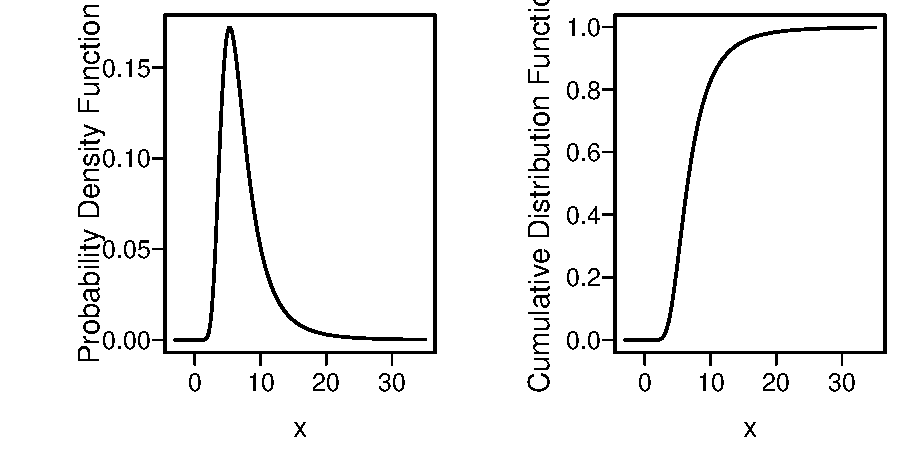
\includegraphics[width=\maxwidth]{descript-pdfcdf-1} }

\caption[Density and cumulative distribution functions]{Example probability density (a) and cumulative probability distribution (b) for a positively skewed random variable (skewed to the right)}\label{fig:descript-pdfcdf}
\end{figure}
\end{Schunk}

\begin{Schunk}
\begin{Sinput}
set.seed(1); x <- rnorm(1000)   # Fig. (*\ref{fig:descript-normalhist}*):
hist(x, nclass=40, prob=TRUE, col=gray(.9), xlab=xl, ylab='')
x <- seq(-4, 4, length=150)
lines(x, dnorm(x, 0, 1), col='blue', lwd=2)
\end{Sinput}
\begin{figure}[htbp]

\centerline{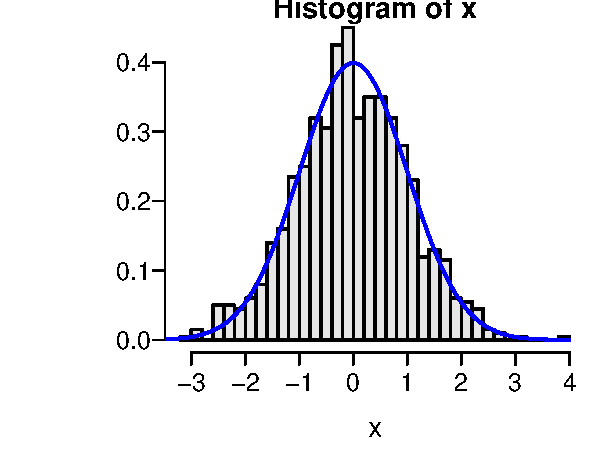
\includegraphics[width=\maxwidth]{descript-normalhist-1} }

\caption[Symmetric continuous distribution]{Example of a continuous distribution that is symmetric: the Gaussian (normal) distribution with mean 0 and variance 1, along with a histogram from a sample of size 1000 from this distribution}\label{fig:descript-normalhist}
\end{figure}
\end{Schunk}

\begin{Schunk}
\begin{Sinput}
set.seed(2)
x <- c(rnorm(500, mean=0, sd=1), rnorm(500, mean=6, sd=3))
hist(x, nclass=40, prob=TRUE, col=gray(.9), xlab=xl, ylab='')
lines(density(x), col='blue', lwd=2)
abline(v=c(0, 6), col='red')   # Fig. (*\ref{fig:descript-bimode}*)
\end{Sinput}
\begin{figure}[htbp]

\centerline{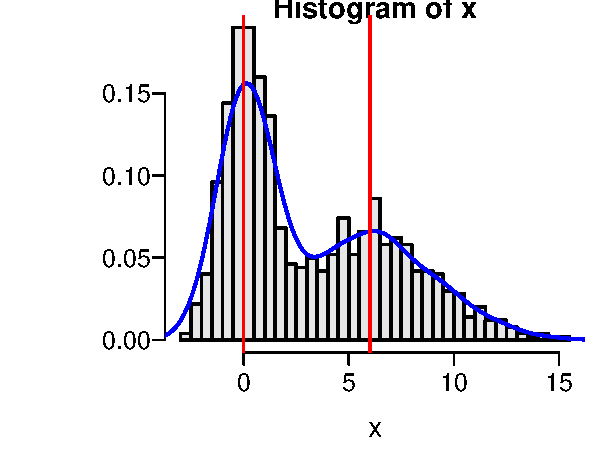
\includegraphics[width=\maxwidth]{descript-bimode-1} }

\caption[Bimodal distribution]{Example of a bimodal distribution from sampling from a mixture of normal distributions with different means and variances and estimating the underlying density function.  Vertical red lines indicate true population means of the two component populations.  Such a distribution can occur naturally or by failing to condition on a binary characteristic such as sex.}\label{fig:descript-bimode}
\end{figure}
\end{Schunk}

\subsection{Ordinal Variables}
\bi
\item Continuous ratio-scaled variables are ordinal
\item Not all ordinal variables are continuous or ratio-scaled
\item Best to analyze ordinal response variables using nonparametric tests or ordinal regression
\item Heavy ties may be present
\item Often better to treat count data as ordinal rather than to assume a distribution such as Poisson or negative binomial that is designed for counts
 \bi
 \item Poisson or negative binomial do not handle extreme clumping at zero
 \ei
\item Example ordinal variables are below
\ei

\begin{Schunk}
\begin{Sinput}
x <- 0:14
y <- c(.8, .04, .03, .02, rep(.01, 11))
plot(x, y, xlab=xl, ylab='', type='n')   # Fig. (*\ref{fig:descript-orda}*)
segments(x, 0, x, y)
\end{Sinput}
\begin{figure}[htbp]

\centerline{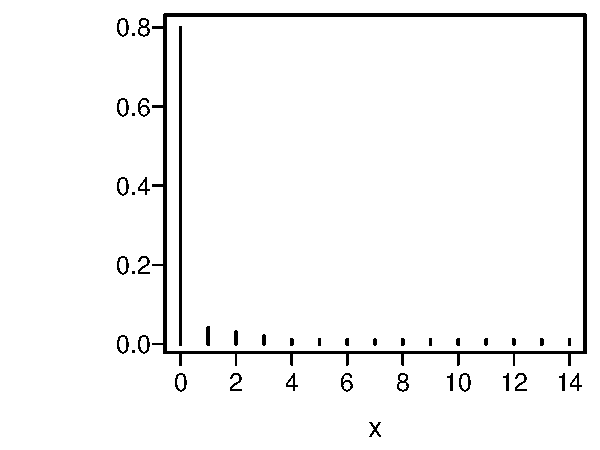
\includegraphics[width=\maxwidth]{descript-orda-1} }

\caption[Count variable with clumping at zero]{Distribution of number of days in the hospital in the year following diagnosis}\label{fig:descript-orda}
\end{figure}
\end{Schunk}
\begin{Schunk}
\begin{Sinput}
x <- 1:10
y <- c(.1, .13, .18, .19, 0, 0, .14, .12, .08, .06)
plot(x, y, xlab=xl, ylab='', type='n')   # Fig. (*\ref{fig:descript-ordb}*)
segments(x, 0, x, y)
\end{Sinput}
\begin{figure}[htbp]

\centerline{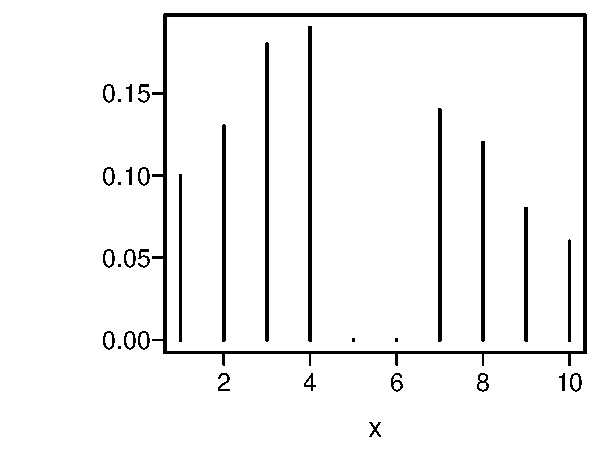
\includegraphics[width=\maxwidth]{descript-ordb-1} }

\caption[Ordinal variable with strange distribution]{Distribution of a functional status score that does not have points in the middle}\label{fig:descript-ordb}
\end{figure}
\end{Schunk}
The \co{getHdata} function in the \co{Hmisc} package~\cite{Hmisc}
finds, downloads, and \co{load()}s datasets from
\href{http://biostat.mc.vanderbilt.edu/wiki/Main/DataSets}{biostat.mc.vanderbilt.edu/DataSets}.
\begin{Schunk}
\begin{Sinput}
require(Hmisc)
getHdata(nhgh)   # NHANES dataset    Fig. (*\ref{fig:descript-ordc}*):
scr <- pmin(nhgh$SCr, 5)   # truncate at 5 for illustration
scr[scr == 5 | runif(nrow(nhgh)) < .05] <- 5  # pretend 1/20 dialyzed
hist(scr, nclass=50, xlab='Serum Creatinine', ylab='Density', prob=TRUE)
\end{Sinput}
\begin{figure}[htbp]

\centerline{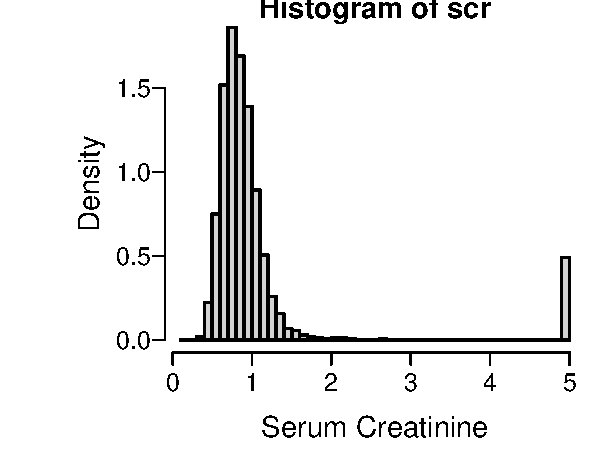
\includegraphics[width=\maxwidth]{descript-ordc-1} }

\caption[Continuous distribution with clumping at the end]{Distribution of serum creatinine where the patient requiring dialysis is taken to have the worst renal function.  The variable is mostly continuous but is best analyzed as ordinal so that no assumption is made about how to score dialysis except for being worse than all non-dialysis patients. Data taken from NHANES where no patients were actually dialyzed.}\label{fig:descript-ordc}
\end{figure}
\end{Schunk}
\clearpage
\section{Descriptive Statistics} \ros{2} \katz{4} \ems{3.2-3.3} \abd{3}
\subsection{Categorical Variables}
\bi
\item Proportions of observations in each category \\
  Note: The mean of a binary variable coded 1/0 is the proportion of
  ones.
\item For variables representing counts (e.g., number of
  comorbidities), the mean is a good summary measure (but not the median)
\item Modal (most frequent) category
\ei

\subsection{Continuous Variables} 
Denote the sample values as $x_{1}, x_{2}, \ldots, x_{n}$
\subsubsection{Measures of Location}
``Center'' of a sample
\bi
\item Mean: arithmetic average
\beq
\bar{x} = \frac{1}{n}\sum_{i=1}^{n}x_{i}
\eeq
Population mean $\mu$ is the long-run average (let $n \rightarrow
\infty$ in computing $\bar{x}$) \\
 \bi
 \item center of mass of the data (balancing point)
 \item highly influenced by extreme values even if they are highly
   atypical
 \ei
\item Median: middle sorted value, i.e., value such that $\frac{1}{2}$
  of the values are below it and above it
 \bi
 \item always descriptive
 \item unaffected by extreme values
 \item not a good measure of central tendency when there are heavy
   ties in the data
 \item if there are heavy ties and the distribution is limited or
   well-behaved, the mean often performs better than the median (e.g.,
   mean number of diseased fingers)
 \ei
\item Geometric mean: hard to interpret and affected by low outliers;
  better to use median
\ei

\subsubsection{Quantiles}
Quantiles are general statistics that can be used to describe central
tendency, spread, symmetry, heavy tailedness, and other quantities.
\bi
\item Sample median: the 0.5 quantile or $50^{th}$ percentile
\item Quartiles $Q_{1}, Q_{2}, Q_{3}$: 0.25 0.5 0.75 quantiles or
  $25^{th}, 50^{th}, 75^{th}$ percentiles
\item Quintiles: by 0.2
\item In general the $p$th sample quantile $x_{p}$ is the value such that a
  fraction $p$ of the observations fall below that value \\
\item $p^{th}$ population quantile: value $x$ such that the
  probability that $X \leq x$ is $p$
\ei

\subsubsection{Spread or Variability}
\bi
\item Interquartile range: $Q_{1}$ to $Q_{3}$ \\
Interval containing $\frac{1}{2}$ of the subjects \\
Meaningful for any continuous distribution
\item Other quantile intervals
\item Variance (for symmetric distributions): averaged squared
  difference between a randomly chosen observation and the mean of all
  observations
\beq
s^{2} = \frac{1}{n-1} \sum_{i=1}^{n} (x_{i} - \bar{x})^2
\eeq
The $-1$ is there to increase our estimate to compensate for our
estimating the center of mass from the data instead of knowing the
population mean.\footnote{$\bar{x}$ is the value of $\mu$ such that
  the sum of squared values about $\mu$ is a minimum.}
\item Standard deviation: $s$ --- $\sqrt{}$ of variance
 \bi 
 \item $\sqrt{}$ of average squared difference of an observation from
   the mean
 \item can be defined in terms of proportion of sample population within
   $\pm$ 1 SD of the mean \textbf{if the population is normal}
 \ei
\item SD and variance are not useful for very asymmetric data,
  e.g. ``the mean hospital cost was \$10000 $\pm$ \$15000''
\item Gini's mean difference: mean absolute difference over all
  possible pairs of observations.  This is highly interpretable. robust, and
  useful for all interval-scaled data, and is even highly precise if
  the data are normal\footnote{Gini's mean difference is labeled
    \co{Gmd} in the output of the \R\ \Co{Hmisc} \co{describe} function,
    and may be computed separately using the \Co{Hmisc} \co{GiniMd} function}.
\item range: not recommended because range $\uparrow$ as $n\uparrow$
  and is dominated by a single outlier
\item coefficient of variation: not recommended (depends too much on
  how close the mean is to zero)
\ei
Example of Gini's mean difference for describing patient-to-patient
variability of systolic blood pressure: If Gini's mean difference is
7mmHg, this means that the average disagreement (absolute difference)
between any two patients is 7mmHg.
\clearpage
\section{Graphics} \label{sec:graphics}\ros{2.8}\katz{4.2-4.6}\altman{17-20}\abd{2,3.4}\bmovie{3}\ddisc{3}
\movie{https://youtu.be/fSgEeI2Xpdc}
Cleveland~\cite{cle94ele,cle84sci} is the best source of how-to
information on making scientific graphs.  Much information may be
found at \url{http://biostat.mc.vanderbilt.edu/StatGraphCourse},
especially these notes: \url{http://goo.gl/DHE0a2}.  Information about
graphics for reporting clinical trials may be found at
\href{http://biostat.mc.vanderbilt.edu/RCTGraphics}{biostat.mc.vanderbilt.edu/RCTGraphics}.  
A link to John Rauser's exceptional video about principles of good graphics
is found on that page as well as in the movie icon in the right margin.


Murrell~\cite{mur13inf} has an excellent summary of recommendations:
\begin{quote}
\bi
\item Display data values using position or length.
\item Use horizontal lengths in preference to vertical lengths.
\item Watch your data--ink ratio.
\item Think very carefully before using color to represent data
  values.
\item Do not use areas to represent data values.
\item \emph{Please} do not use angles or slopes to represent data
  values.
\item \emph{Please, please} do not use volumes to represent data
  values.
\ei
\end{quote}

On the fifth point above, avoid the use of \emph{bars} when
representing a single number.  Bar widths contain no information and
get in the way of important information.  This is addressed below.

\R\ has superior graphics implemented in multiple models, including
\bi
\item Base graphics such as \Co{plot(), hist(), lines(), points()}
  which give the user maximum control and are best used when not
  stratifying by additional variables other than the ones being summarized
\item The \Co{lattice} package which is fast but not quite as good as
  \Co{ggplot2} when one needs to vary more than one of color, symbol,
  size, or line type due to having more than one categorizing variable
\item The \Co{ggplot2} package which is very flexible and has the
  nicest defaults especially for constructing keys (legends/guides)
\item For semi-interactive graphics inserted into html reports, the
  \R\ \Co{plotly} package, which uses the \Co{plotly} system
  (which uses the Javascript \Co{D3} library) is extremely powerful.
  See \url{https://plot.ly/r/getting-started}. 
\item Fully interactive graphics can be built using \Co{RShiny} but
  this requires a server to be running while the graph is viewed.
\ei

For \Co{ggplot2}, \url{http://www.cookbook-r.com/Graphs} contains a
nice cookbook.  See also \url{http://learnr.wordpress.com}.  To get
excellent documentation with examples for any 
\Co{ggplot2} function, google \Co{ggplot2 \emph{functionname}}.
\Co{ggplot2} graphs can be converted into \Co{plotly} graphics using
the \Co{ggplotly} function.  But you will have more control using
\R\ \Co{plotly} directly.

The older non-interactive graphics models which are useful for
producing printed and \Co{pdf} output are starting to be superceded
with interactive graphics.  One of the biggest advantages of the
latter is the ability to present the most important graphic
information front-and-center but to allow the user to easily hover the
mouse over areas in the graphic to see tabular details.


\subsection{Graphing Change vs.\ Raw Data}\alabel{sec:descript-change}
A common mistake in scientific graphics is to cover up subject
variability by normalizing repeated measures for baseline (see
Section~\ref{sec:overview-preprocessing}).  Among other problems, this
prevents the reader from seeing regression to the mean for subjects
starting out at very low or very high values, and from seeing
variation in intervention effect as a function of baseline values.  It
is highly recommended that all the raw data be shown, including those
from time zero.  When the sample size is not huge, spaghetti plots are
most effective for graphing longitudinal data because all points from
the same subject over time are connected.  An
example~\citep{davis-repmeas}{pp.\ 161-163} is below. 
\begin{Schunk}
\begin{Sinput}
require(Hmisc)   # also loads ggplot2
getHdata(cdystonia)
ggplot(cdystonia, aes(x=week, y=twstrs, color=factor(id))) +
       geom_line() + xlab('Week') + ylab('TWSTRS-total score') +
       facet_grid(treat ~ site) +
       guides(color=FALSE) # Fig. (*\ref{fig:descript-spaghetti}*)
\end{Sinput}
\begin{figure}[htbp]

\centerline{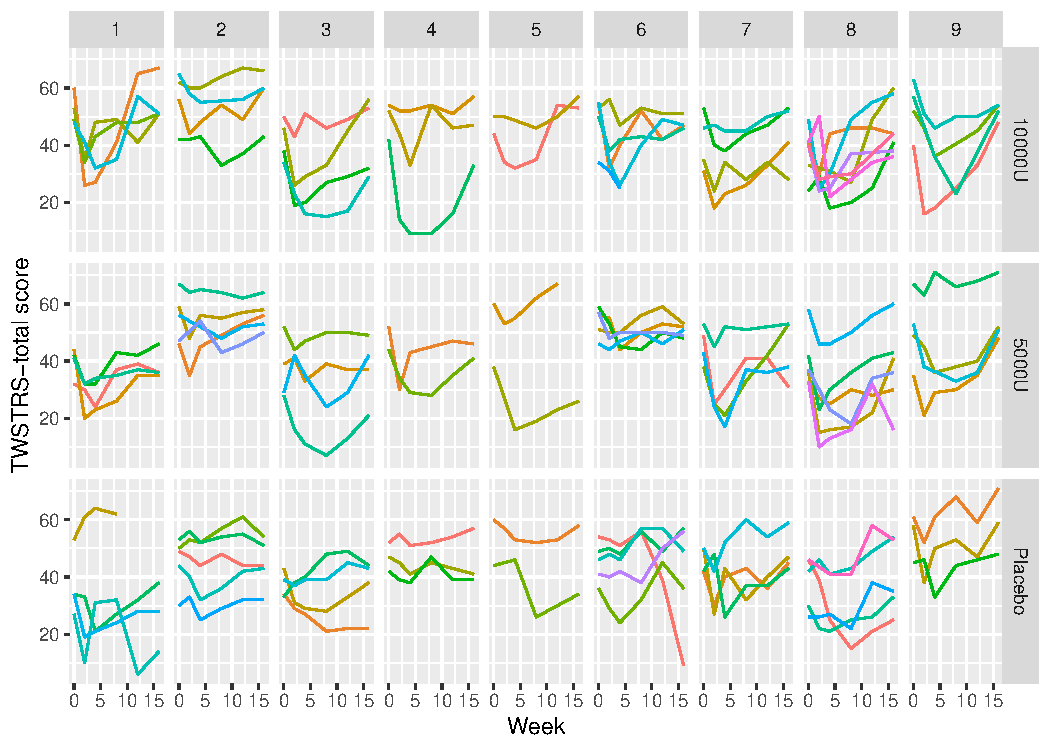
\includegraphics[width=\maxwidth]{descript-spaghetti-1} }

\caption[Spaghetti plot]{Spaghetti plot showing all the raw data on the response variable for each subject, stratified by dose and study site (1--9).  Importantly, week 0 (baseline) measurements are included.}\label{fig:descript-spaghetti}
\end{figure}
\end{Schunk}
Graphing the raw data is usually essential.

\subsection{Categorical Variables}
\bi
\item pie chart
 \bi
 \item high ink:information ratio
 \item optical illusions (perceived area or angle depends on
   orientation vs.\ horizon)
 \item hard to label categories when many in number
 \ei
\item bar chart
 \bi
 \item high ink:information ratio
 \item hard to depict confidence intervals (one sided error bars?)
 \item hard to interpret if use subcategories
 \item labels hard to read if bars are vertical
 \ei
\item dot chart
 \bi
 \item leads to accurate perception
 \item easy to show all labels; no caption needed
 \item allows for multiple levels of categorization (see Figures \ref{fig:descript-counts-dotchart} and \ref{desc-proportions-txreg})
 
\begin{Schunk}
\begin{Sinput}
getHdata(titanic3)
d <- upData(titanic3,
            agec     = cut2(age, c(10, 15, 20, 30)), print=FALSE)
d <- with(d, as.data.frame(table(sex, pclass, agec)))
d <- subset(d, Freq > 0)
ggplot(d, aes(x=Freq, y=agec)) + geom_point() +
  facet_grid(sex ~ pclass) +
  xlab('Frequency') + ylab('Age')
\end{Sinput}
\begin{figure}[htbp]

\centerline{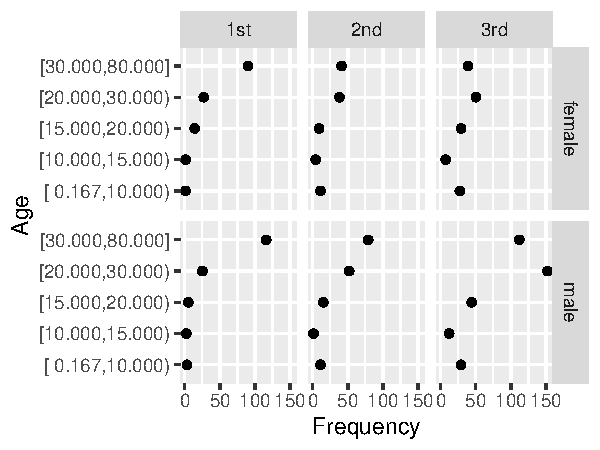
\includegraphics[width=\maxwidth]{descript-counts-dotchart-1} }

\caption[Frequency dot chart]{Dot chart showing frequencies from cross-classifications of discrete variables for Titanic passengers}\label{fig:descript-counts-dotchart}
\end{figure}
\end{Schunk}

\figs{desc-proportions-txreg}{Dot chart for categorical demographic
  variables, stratified by treatment and region}{1}

\figs{aevents}{Dot chart showing proportion of subjects having adverse
  events by treatment, sorted by risk difference, produced by the \R\
  \co{greport} package.  See \co{test.Rnw}
  at \protect\url{biostat.mc.vanderbilt.edu/Greport}}{1}

  \bi
  \item multi-panel display for multiple major categorizations
  \item lines of dots arranged vertically within panel
  \item categories within a single line of dots
  \ei
 \item easy to show 2-sided error bars
 \ei
\item Avoid chartjunk such as dummy dimensions in bar charts, rotated
  pie charts, use of solid areas when a line suffices
\ei

\subsection{Continuous Variables}
\subsubsection{Raw Data}
For graphing two continuous variable, scatterplots are often
essential.  The following example draws a scatterplot on a very large
number of observations in a measurement comparison study where the
goal is to measure esophageal pH longitudinally and across subjects.
\begin{Schunk}
\begin{Sinput}
getHdata(esopH)
contents(esopH)
\end{Sinput}
\begin{Soutput}

Data frame:esopH	136127 observations and 2 variables    Maximum # NAs:0


                                       Labels   Class Storage
orophar Esophageal pH by Oropharyngeal Device numeric  double
conv     Esophageal pH by Conventional Device numeric  double
\end{Soutput}
\begin{Sinput}
xl <- label(esopH$conv)
yl <- label(esopH$orophar)
ggplot(esopH, aes(x=conv, y=orophar)) + geom_point(pch='.') +
  xlab(xl) + ylab(yl) +   # Fig. (*\ref{fig:descript-pH}*)
  geom_abline(intercept = 0, slope = 1)
\end{Sinput}
\begin{figure}[htbp]

\centerline{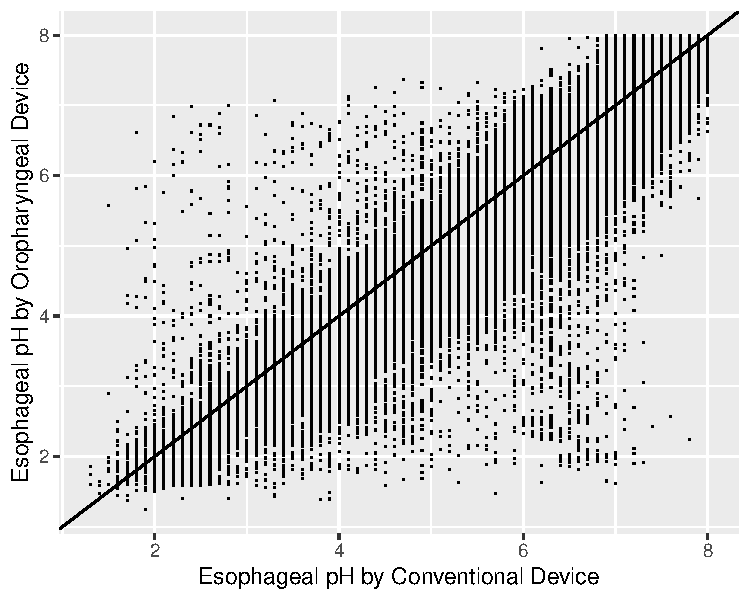
\includegraphics[width=\maxwidth]{descript-pH-1} }

\caption[Scatterplot of one measurement mode against another]{Scatterplot of one measurement mode against another}\label{fig:descript-pH}
\end{figure}
\end{Schunk}
With large sample sizes there are many collisions of data points and
hexagonal binning is an effective substitute for the raw
data scatterplot.  The number of points represented by one hexagonal
symbol is stratified into 20 groups of approximately equal numbers of
points.  The code below is not currently working for the \co{ggplot2}
package version 2.1.0. 
\begin{Schunk}
\begin{Sinput}
ggplot(esopH, aes(x=conv, y=orophar)) +
  stat_binhex(aes(alpha=..count.., color=Hmisc::cut2(..count.., g=20)),
              bins=80) +
  xlab(xl) + ylab(yl) +
  guides(alpha=FALSE, fill=FALSE, color=guide_legend(title='Frequency'))
\end{Sinput}
\end{Schunk}
Instead we use the \Co{Hmisc} \co{ggfreqScatter} function to bin the
points and represent frequencies of overlapping points with color and
transparency levels. 
\begin{Schunk}
\begin{Sinput}
with(esopH, ggfreqScatter(conv, orophar, bins=50, g=20) +
              geom_abline(intercept=0, slope=1))   # Fig. (*\ref{fig:descript-pHh2}*)
\end{Sinput}
\begin{figure}[htbp]

\centerline{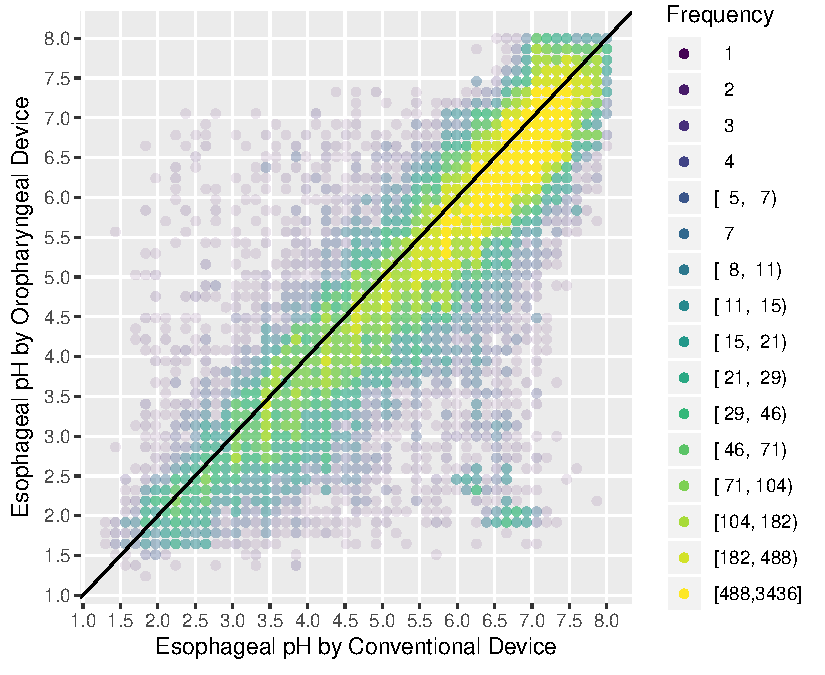
\includegraphics[width=\maxwidth]{descript-pHh2-1} }

\caption[Binned points (2500 total bins) with frequency counts shown as color and transparency level]{Binned points (2500 total bins) with frequency counts shown as color and transparency level}\label{fig:descript-pHh2}
\end{figure}
\end{Schunk}

\subsubsection{Distributions}\abd{1.4}\label{sec:desc-dist}
\bi
\item histogram showing relative frequencies
 \bi
 \item requires arbitrary binning of data
 \item not optimal for comparing multiple distributions
 \ei
\item cumulative distribution function: proportion of values $\leq x$
  vs.\ $x$ (Figure \ref{fig:descript-ecdf}) \\
 Can read all quantiles directly off graph.
\begin{Schunk}
\begin{Sinput}
getHdata(pbc)
pbcr <- subset(pbc, drug != 'not randomized')
Ecdf(pbcr[,c('bili','albumin','protime','sgot')],  # Fig. (*\ref{fig:descript-ecdf}*)
    group=pbcr$drug, col=1:2,
    label.curves=list(keys='lines'))
\end{Sinput}
\begin{figure}[htbp]

\centerline{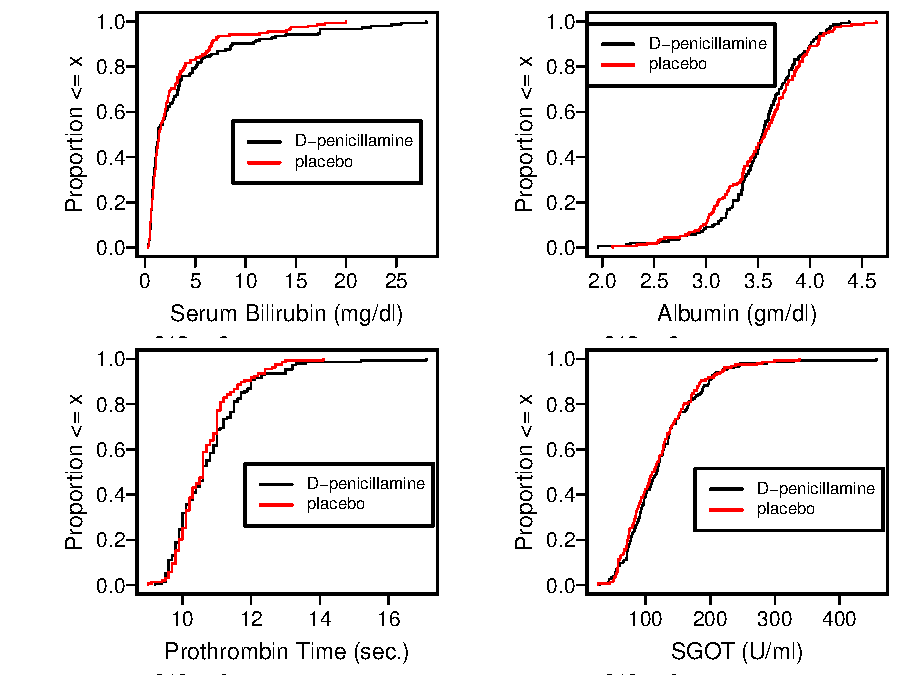
\includegraphics[width=\maxwidth]{descript-ecdf-1} }

\caption[Empirical cumulative distribution functions]{Empirical cumulative distributions of baseline variables  stratified by treatment in a randomized controlled trial. $m$ is the number of missing values.}\label{fig:descript-ecdf}
\end{figure}
\end{Schunk}

\item Box plots shows quartiles plus the mean.  They are a good way to
  compare many groups as seen in Figures~\ref{fig:descript-bwplot} and
  \ref{fig:descript-glybox}. 
\begin{Schunk}
\begin{Sinput}
getHdata(support)   # Fig. (*\ref{fig:descript-bwplot}*)
bwplot(dzgroup ~ crea, data=support, panel=panel.bpplot,
       probs=c(.05,.25), xlim=c(0,8), xlab='Serum Creatinine')
\end{Sinput}
\begin{figure}[htbp]

\centerline{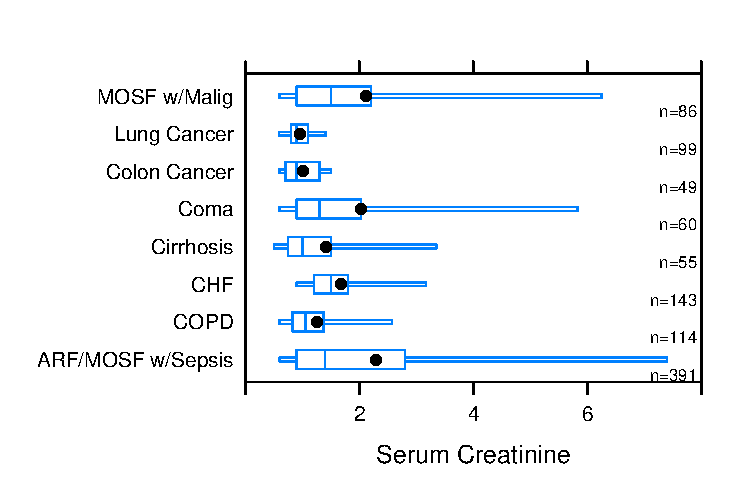
\includegraphics[width=\maxwidth]{descript-bwplot-1} }

\caption[Box plots with 0.05 and 0.95 quantiles]{Box plots showing the distribution of serum creatinine  stratified by major diagnosis.  Dot: mean; vertical line: median; large box:interquartile range.  The 0.05 and 0.95 quantiles are also shown, which is not the way typical box plots are drawn but is perhaps more useful.  Asymmetry of distributions can be seen by both disagreement between $Q_{3}-Q_{2}$ and $Q_{2}-Q_{1}$ and by disagreement between $Q_{2}$ and $\bar{x}$.}\label{fig:descript-bwplot}
\end{figure}
\end{Schunk}

Figure \ref{fig:descript-glybox} uses extended box plots.  The
following schematic shows how to interpret them.
\begin{Schunk}
\begin{Sinput}
bpplt()   # Fig. (*\ref{fig:descript-bpplt}*)
\end{Sinput}
\begin{figure}[htbp]

\centerline{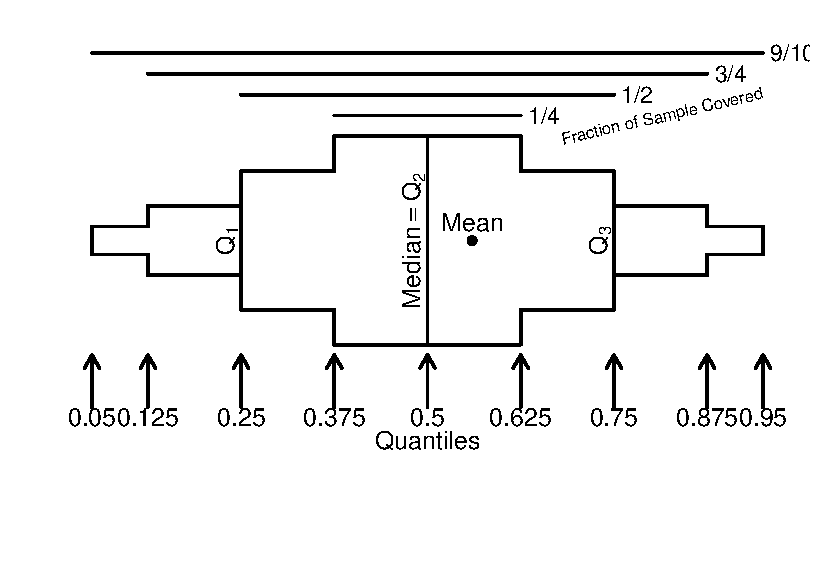
\includegraphics[width=\maxwidth]{descript-bpplt-1} }

\caption[Schematic for extended box plot]{Schematic for extended box plot}\label{fig:descript-bpplt}
\end{figure}
\end{Schunk}

\begin{Schunk}
\begin{Sinput}
require(lattice)   # Fig. (*\ref{fig:descript-glybox}*):
getHdata(diabetes)
wst <- cut2(diabetes$waist, g=2)
levels(wst) <- paste('Waist', levels(wst))
bwplot(cut2(age,g=4) ~ glyhb | wst*gender, data=diabetes,
       panel=panel.bpplot, xlab='Glycosylated Hemoglobin', ylab='Age Quartile')
\end{Sinput}
\begin{figure}[htbp]

\centerline{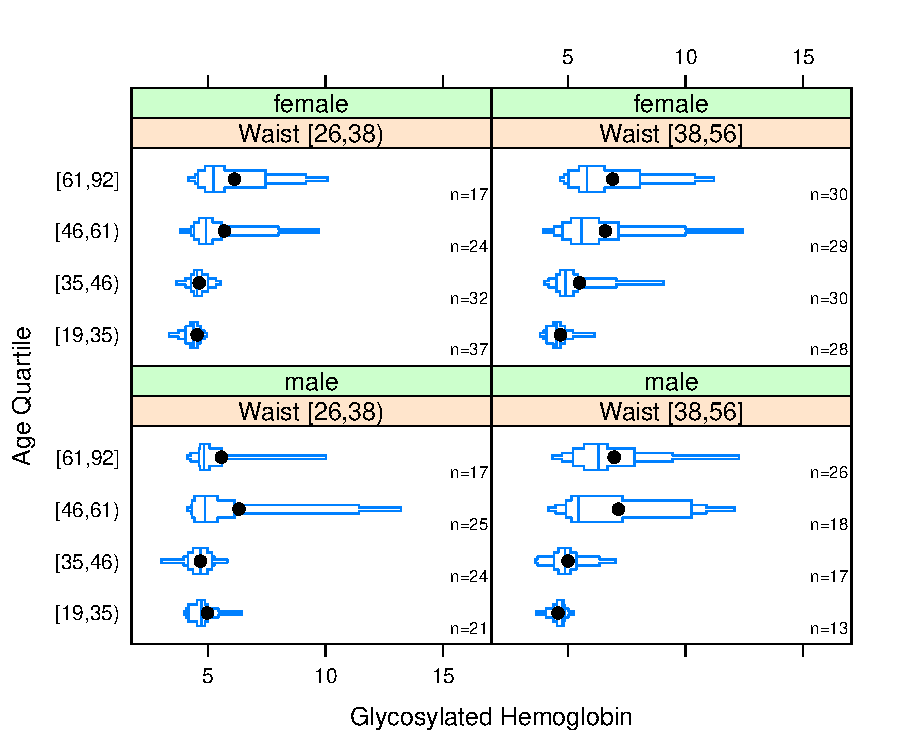
\includegraphics[width=\maxwidth]{descript-glybox-1} }

\caption[Extended box plots for glycohemoglobin]{Extended box plots for glycohemoglobin stratified by quartiles of age (vertical), two-tiles of waist circumference (horizontal), and sex (vertical)}\label{fig:descript-glybox}
\end{figure}
\end{Schunk}

Box plots are inadequate for displaying bimodality.  Violin plots show
the entire distribution well if the variable being summarized is
fairly continuous.

\figs{cchem-byx-cont-a}{One-half violin plots for longitudinal data, stratified
  by treatment.  Density estimates for groups with insufficient sample
  sizes are faded.  Density plots are back--to--back for treatment A
  and B.  Points are treatment medians.  When the black vertical line
  does not touch the two medians, the medians are significantly
  different at the $\alpha=0.05$ level.  Graphic was produced by the
  \R\ \Co{greport} package.}{1}
\ei


\subsubsection{Relationships}
\bi
\item When response variable is continuous and descriptor
  (stratification) variables are categorical, multi-panel dot charts,
  box plots, multiple cumulative distributions, etc., are useful.
\item Two continuous variables: scatterplot\ems{~Figure~3.9}
% also Rosner Figure 2.12
\ei


\subsection{Graphs for Summarizing Results of Studies}
\bi
\item Dot charts with optional error bars (for confidence limits) can
  display any summary statistic (proportion, mean, median, mean
  difference, etc.)
\item It is not well known that the confidence interval for a
  difference in two means cannot be derived from individual confidence
  limits.\footnote{In addition, it is not necessary for two confidence
    intervals to be separated for the difference in means to be
    significantly different from zero.} \\
  Show individual confidence limits as well as actual CLs for the
  difference.
\begin{Schunk}
\begin{Sinput}
attach(diabetes)
set.seed(1)
male   <- smean.cl.boot(glyhb[gender=='male'],   reps=TRUE)
female <- smean.cl.boot(glyhb[gender=='female'], reps=TRUE)
dif <- c(mean=male['Mean']-female['Mean'],
         quantile(attr(male, 'reps')-attr(female,'reps'), c(.025,.975)))
plot(0,0,xlab='Glycated Hemoglobin',ylab='',   # Fig. (*\ref{fig:descript-cldif}*)
     xlim=c(5,6.5),ylim=c(0,4), axes=F)
axis(1, at=seq(5, 6.5, by=0.25))
axis(2, at=c(1,2,3.5), labels=c('Female','Male','Difference'),
     las=1, adj=1, lwd=0)
points(c(male[1],female[1]), 2:1)
segments(female[2], 1, female[3], 1)
segments(male[2], 2,   male[3], 2)
offset <- mean(c(male[1],female[1])) - dif[1]
points(dif[1] + offset, 3.5)
segments(dif[2]+offset, 3.5, dif[3]+offset, 3.5)
at <- c(-.5,-.25,0,.25,.5,.75,1)
axis(3, at=at+offset, label=format(at))
segments(offset, 3, offset, 4.25, col=gray(.85))
abline(h=c(2 + 3.5)/2, col=gray(.85))
\end{Sinput}
\begin{figure}[htbp]

\centerline{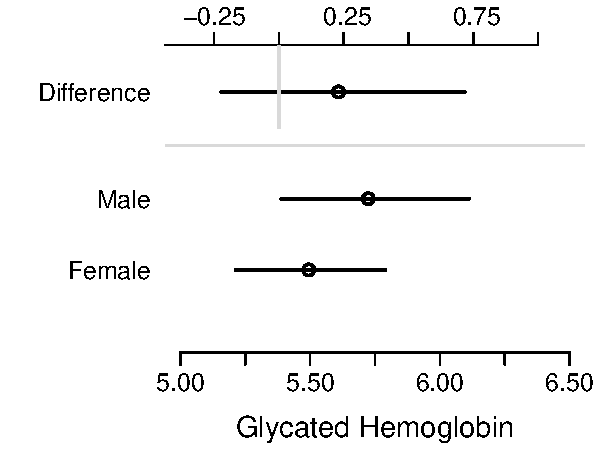
\includegraphics[width=\maxwidth]{descript-cldif-1} }

\caption[Showing group means and differences]{Means and nonparametric bootstrap 0.95 confidence limits for glycated hemoglobin for males and females, and confidence limits for males - females.  Lower and upper $x$-axis scales have same spacings but different centers.  Confidence intervals for differences are generally wider than those for the individual constituent variables.}\label{fig:descript-cldif}
\end{figure}
\end{Schunk}
  
\item For showing relationship between two continuous variables, a
  trend line or regression model fit, with confidence bands
\ei

\subsubsection{Bar Plots with Error Bars}

\bi
\item ``Dynamite'' Plots
\item Height of bar indicates mean, lines represent standard error
\item High ink:information ratio
\item Hide the raw data, assume symmetric confidence intervals
\item Replace with
  \bi
   \item Dot plot (smaller sample sizes)
   \item Box plot (larger sample size)
  \ei
\ei
\begin{Schunk}
\begin{Sinput}
getHdata(FEV); set.seed(13)   
FEV <- subset(FEV, runif(nrow(FEV)) < 1/8)   # 1/8 sample
require(ggplot2)
s <- with(FEV, summarize(fev, llist(sex, smoke), smean.cl.normal))
ggplot(s, aes(x=smoke, y=fev, fill=sex)) +    # Fig. (*\ref{fig:descript-dynamite}*)
    geom_bar(position=position_dodge(), stat="identity") +
    geom_errorbar(aes(ymin=Lower, ymax=Upper),
                  width=.1,
                  position=position_dodge(.9))
\end{Sinput}
\begin{figure}[htbp]

\centerline{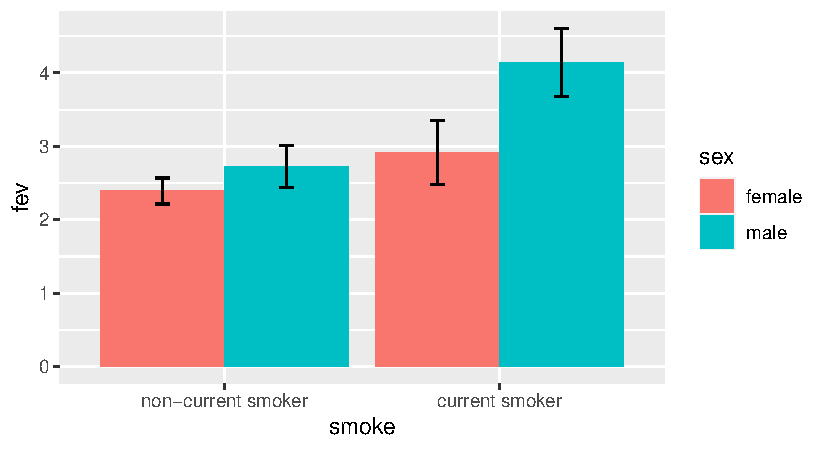
\includegraphics[width=\maxwidth]{descript-dynamite-1} }

\caption[Bar plot with error bars---``dynamite plot'']{Bar plot with error bars---``dynamite plot''}\label{fig:descript-dynamite}
\end{figure}
\end{Schunk}
See \url{http://biostat.mc.vanderbilt.edu/DynamitePlots} for a list of
the many problems caused by dynamite plots, plus some solutions.

Instead of the limited information shown in the bar chart, show the
raw data along with box plots.  Modify default box plots to replace
whiskers with the interval between 0.1 and 0.9 quantiles.
\begin{Schunk}
\begin{Sinput}
require(ggplot2)   # Fig. (*\ref{fig:descript-tplot}*)
stats <- function(x) {
  z <- quantile(x, probs=c(.1, .25, .5, .75, .9))
  names(z) <- c('ymin', 'lower', 'middle', 'upper', 'ymax')
  if(length(x) < 10) z[c(1,5)] <- NA
  z
}
ggplot(FEV, aes(x=sex, y=fev)) +
  stat_summary(fun.data=stats, geom='boxplot', aes(width=.75), shape=5,
               position='dodge', col='lightblue') +
  geom_dotplot(binaxis='y', stackdir='center', position='dodge', alpha=.4) +
  stat_summary(fun.y=mean, geom='point', shape=5, size=4, color='blue') +
  facet_grid(~ smoke) +
  xlab('') + ylab(expression(FEV[1])) + coord_flip()
\end{Sinput}
\begin{figure}[htbp]

\centerline{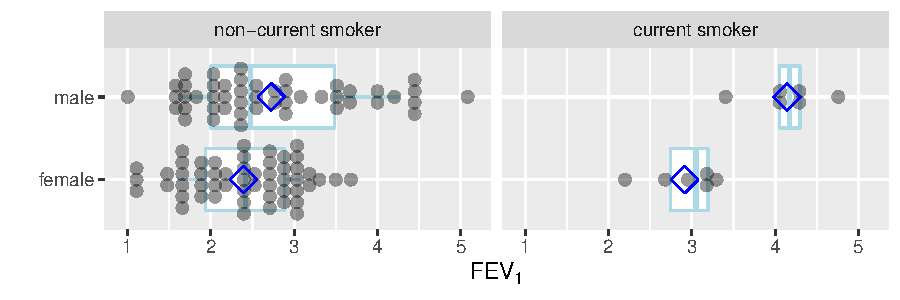
\includegraphics[width=\maxwidth]{descript-tplot-1} }

\caption[Dot plot with superimposed box plots]{Jittered raw data and box plots.  Middle vertical lines indicate medians and diamonds indicate means. Horizontal lines indicate 0.1 to 0.9 quantiles when $n\geq 10$.  The ink:information ratio for this plot is far better than a dynamite plot.}\label{fig:descript-tplot}
\end{figure}
\end{Schunk}
Use a violin plot to show the distribution density estimate (and its
mirror image) instead of a box plot.
\begin{Schunk}
\begin{Sinput}
ggplot(FEV, aes(x=sex, y=fev)) +
  geom_violin(width=.6, col='lightblue') +
  geom_dotplot(binaxis='y', stackdir='center', position='dodge', alpha=.4) +
  stat_summary(fun.y=median, geom='point', color='blue', shape='+', size=12) +
  facet_grid(~ smoke) +
  xlab('') + ylab(expression(FEV[1])) + coord_flip()
\end{Sinput}
\begin{figure}[htbp]

\centerline{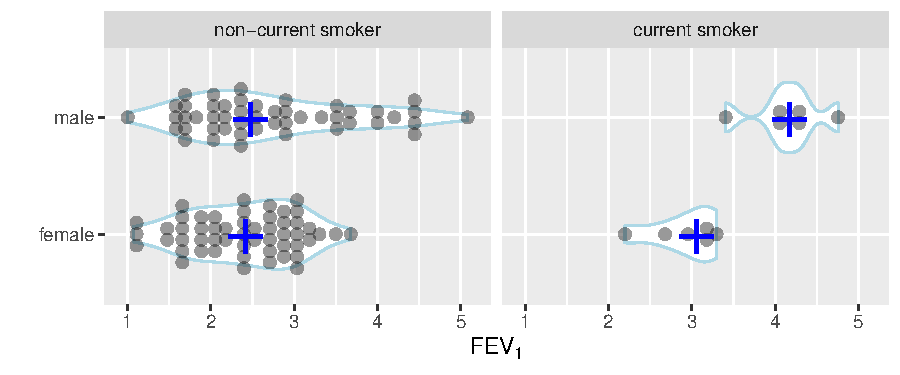
\includegraphics[width=\maxwidth]{descript-vplot-1} }

\caption[Jittered raw data and violin plots with median indicated by \textbf{\textcolor{blue}{+}}]{Jittered raw data and violin plots with median indicated by \textbf{\textcolor{blue}{+}}}\label{fig:descript-vplot}
\end{figure}
\end{Schunk}

% Was
% ggplot(FEV, aes(x=smoke, y=fev, color=sex)) +
%   geom_boxplot(alpha=.5, width=.2) + # remove width to overlay boxes on pts
%   stat_summary(fun.y=mean, geom="point", shape=5, size=2, 
%                position=position_dodge(width=.15)) +
%   geom_dotplot(binaxis='y', stackdir='center', position='dodge') +
%   xlab('') + ylab(expression(FEV[1])) + coord_flip() 
% ggplot(FEV, aes(x=smoke, y=fev, color=sex)) +
%   stat_summary(fun.data=stats, geom='boxplot', shape=5, position='dodge') +
%   geom_dotplot(binaxis='y', stackdir='center', position='dodge') +
%   stat_summary(fun.y=mean, geom="point", shape=5, size=2, 
%                position=position_dodge(width=.2)) +
%   xlab('') + ylab(expression(FEV[1])) + coord_flip()
  
%## Define Tatsuki Koyama's tplot function
%base <- 'http://biostat.mc.vanderbilt.edu/wiki/pub/Main'
%source(paste(base, 'TatsukiRcode/TatsukiRcodeTplot.R', sep='/'))
%par(mar=c(4,9,1,4))
%tplot(fev ~ smoke, data=FEV, show.n=TRUE, bty='L', type='db',
%      pch=20, las=1, mean.line=TRUE, horizontal=TRUE, ylab='FEV1',
%      col=c(female='darkred',male='darkblue')[as.character(FEV$sex)],
%      dist=.02, boxcol='lightyellow1', boxborder=gray(.8))  # Fig. (*\ref{fig:descript-tplot}*)

\subsubsection{Semi-Interactive Graphics Examples}

These examples are all found in \url{hbiostat.org/talks/rmedicine19.html}.

\bi
\item \href{https://hbiostat.org/talks/rmedicine19.html}{R for
  Clinical Trial Reporting}
\item \href{https://hbiostat.org/talks/rmedicine19.html#11}{Spike
  histograms with hovertext for overall statistical summary} (slide 11)
\item \href{https://hbiostat.org/talks/rmedicine19.html#12}{Dot plots}
  (slide 12)
\item \href{https://hbiostat.org/talks/rmedicine19.html#13}{Extended
  box plots} (slide 13)
\item \href{https://hbiostat.org/talks/rmedicine19.html#15}{Spike
  histograms with quantiles, mean, dispersion} (slide 15)
\item \href{https://hbiostat.org/talks/rmedicine19.html#16}{Survival
  plots with CI for difference, continuous number at risk} (slide 16)
\item \href{https://hbiostat.org/talks/rmedicine19.html#35}{Example
  clinical trial reports} (slide 35)
\ei

Other examples: descriptions of BBR course participants: \href{https://hbiostat.org/bbr/registrants.html}{hbiostat.org/bbr/registrants.html}.


\subsection{Graphs for Describing Statistical Model Fits}
Several types of graphics are useful.  These are all implemented in
the \R\ \Co{rms} package~\cite{rrms}.
\begin{description}
  \item[Partial effect plots]: Show the effect on $Y$ of varying one
    predictor at a time, holding the other predictors to medians or
    modes, and include confidence bands.  This is the best approach
    for showing shapes of effects of continuous predictors.
  \item[Effect charts]: Show the difference in means, odds ratio,
    hazard ratio, fold change, etc., varying each predictor and
    holding others to medians or modes\footnote{It does not matter
      what the other variables are set to if they do not interact with
      the variable being varied.}.  For continuous variables that do
    not operate linearly, this kind of display is not very
    satisfactory because of its strong dependence on the settings over
    which the predictor is set.  By default inter-quartile-range
    effects are used.
  \item[Nomograms]: Shows the entire model if the number of
    interactions is limited.  Nomograms show strengths and shapes of
    relationships, are very effective for continuous predictors, and
    allow computation of predicted values (although without confidence limits).
\end{description}
Here are examples using NHANES data to predict glycohemoglobin from
age, sex, race/ethnicity, and BMI.\\
\textbf{Note}: ordinary regression is not an adequate fit for glycohemoglobin;
an excellent fit comes from ordinal regression.  BMI is not an
adequate summary of body size.  The following
ordinary regression model in the $-1.75$ power of glycohemoglobin
resulted in approximately normal residuals and is used for
illustration.  The transformation is subtracted from a constant just
so that positive regression coefficients indicate that increasing a
predictor increases glycohemoglobin.  The inverse transformation
raises predicted values to 
the $-\frac{1}{1.75}$ power after accounting for the subtraction, and
is used to estimate the median glycohemoglobin on 
the original scale\footnote{If residuals have a normal distribution
  after transforming the dependent variable, the estimated mean and
  median transformed values are the same.  Inverse transforming the
  estimates provides an estimate of the median on the original scale
  (but not the mean).}.  Restricted cubic spline 
functions with 4 default 
knots are used to allow age and BMI to act smoothly but nonlinearly.
Partial effects plots are in Fig.~\ref{fig:descript-rmsa}.
\begin{Sinput}
require(rms)
getHdata(nhgh)   # NHANES data
dd <- datadist(nhgh); options(datadist='dd')
g        <- function(x) 0.09 - x ^ - (1 / 1.75)
ginverse <- function(y) (0.09 - y) ^ -1.75
f <- ols(g(gh) ~ rcs(age, 4) + re + sex + rcs(bmi, 4), data=nhgh)
cat('{\\small\n')
\end{Sinput}
{\small
\begin{Sinput}
f
\end{Sinput}

 \centerline{\textbf{Linear Regression Model}}
 
 \begin{verbatim}
 ols(formula = g(gh) ~ rcs(age, 4) + re + sex + rcs(bmi, 4), data = nhgh)
 \end{verbatim}
 
 {\fontfamily{phv}\selectfont \begin{center}\begin{tabular}{|c|c|c|}\hline
&Model Likelihood&Discrimination\\
&Ratio Test&Indexes\\\hline
Obs~\hfill 6795&LR $\chi^{2}$~\hfill 1861.16&$R^{2}$~\hfill 0.240\\
$\sigma$~\hfill 0.0235&d.f.~\hfill 11&$R^{2}_{\textrm{adj}}$~\hfill 0.238\\
d.f.~\hfill 6783&Pr$(>\chi^{2})$~\hfill 0.0000&$g$~\hfill 0.015\\
\hline
\end{tabular}
\end{center}}
 \begin{center}
 Residuals
 

 \begin{tabular}{ccccc}
Min&1Q&Median&3Q&Max\\
$-0.09736$&$-0.01208$&$-0.002201$&$0.008237$&$0.1689$\\
\end{tabular}
 \end{center}
 
 %latex.default(U, file = "", first.hline.double = FALSE, table = FALSE,     longtable = TRUE, lines.page = lines.page, col.just = rep("r",         ncol(U)), rowlabel = "", already.math.col.names = TRUE,     append = TRUE)%
 \setlongtables\begin{longtable}{lrrrr}\hline
 \multicolumn{1}{l}{}&\multicolumn{1}{c}{$\hat{\beta}$}&\multicolumn{1}{c}{S.E.}&\multicolumn{1}{c}{$t$}&\multicolumn{1}{c}{Pr$(>|t|)$}\tabularnewline
 \hline
 \endhead
 \hline
 \endfoot
 Intercept&~-0.2884~&~0.0048~&-60.45&\textless 0.0001\tabularnewline
 age&~ 0.0002~&~0.0001~&  3.34&0.0008\tabularnewline
 age'&~ 0.0010~&~0.0001~&  7.63&\textless 0.0001\tabularnewline
 age''&~-0.0040~&~0.0005~& -8.33&\textless 0.0001\tabularnewline
 re=Other Hispanic&~-0.0013~&~0.0011~& -1.20&0.2318\tabularnewline
 re=Non-Hispanic White&~-0.0082~&~0.0008~&-10.55&\textless 0.0001\tabularnewline
 re=Non-Hispanic Black&~-0.0013~&~0.0009~& -1.34&0.1797\tabularnewline
 re=Other Race Including Multi-Racial&~ 0.0006~&~0.0014~&  0.47&0.6411\tabularnewline
 sex=female&~-0.0022~&~0.0006~& -3.90&\textless 0.0001\tabularnewline
 bmi&~-0.0006~&~0.0002~& -2.54&0.0111\tabularnewline
 bmi'&~ 0.0059~&~0.0009~&  6.44&\textless 0.0001\tabularnewline
 bmi''&~-0.0161~&~0.0025~& -6.40&\textless 0.0001\tabularnewline
 \hline
 \end{longtable}
 \addtocounter{table}{-1}
\begin{Sinput}
print(anova(f), dec.ss=3, dec.ms=3)
\end{Sinput}
%latex.default(dstats, title = title, caption = if (table.env) caption else NULL,     insert.top = if (length(caption) && !table.env) paste0("\\Needspace{2in}\n",         caption), rowlabel = "", col.just = rep("r", length(sn)),     table.env = table.env, ...)%
\textbf{\Needspace{2in}
Analysis of Variance for \texttt{\smaller g(gh)}}\begin{center}
\begin{tabular}{lrrrrr}
\hline\hline
\multicolumn{1}{l}{}&\multicolumn{1}{c}{d.f.}&\multicolumn{1}{c}{Partial SS}&\multicolumn{1}{c}{MS}&\multicolumn{1}{c}{$F$}&\multicolumn{1}{c}{$P$}\tabularnewline
\hline
age&   3&0.732&0.244&441.36&\textless 0.0001\tabularnewline
~~\emph{Nonlinear}&   2&0.040&0.020& 35.83&\textless 0.0001\tabularnewline
re&   4&0.096&0.024& 43.22&\textless 0.0001\tabularnewline
sex&   1&0.008&0.008& 15.17&\textless 0.0001\tabularnewline
bmi&   3&0.184&0.061&110.79&\textless 0.0001\tabularnewline
~~\emph{Nonlinear}&   2&0.023&0.011& 20.75&\textless 0.0001\tabularnewline
TOTAL NONLINEAR&   4&0.068&0.017& 30.94&\textless 0.0001\tabularnewline
\textbf{REGRESSION}&  11&1.181&0.107&194.29&\textless 0.0001\tabularnewline
\textbf{ERROR}&6783&3.749&0.001&&\tabularnewline
\hline
\end{tabular}\end{center}
\begin{Sinput}
cat('}\n')
\end{Sinput}
}
\begin{Sinput}
# Show partial effects of all variables in the model, on the original scale
ggplot(Predict(f, fun=ginverse),   # Fig. (*\ref{fig:descript-rmsa}*)
       ylab=expression(paste('Predicted Median ', HbA['1c'])))
\end{Sinput}
\begin{figure}[htbp]

\centerline{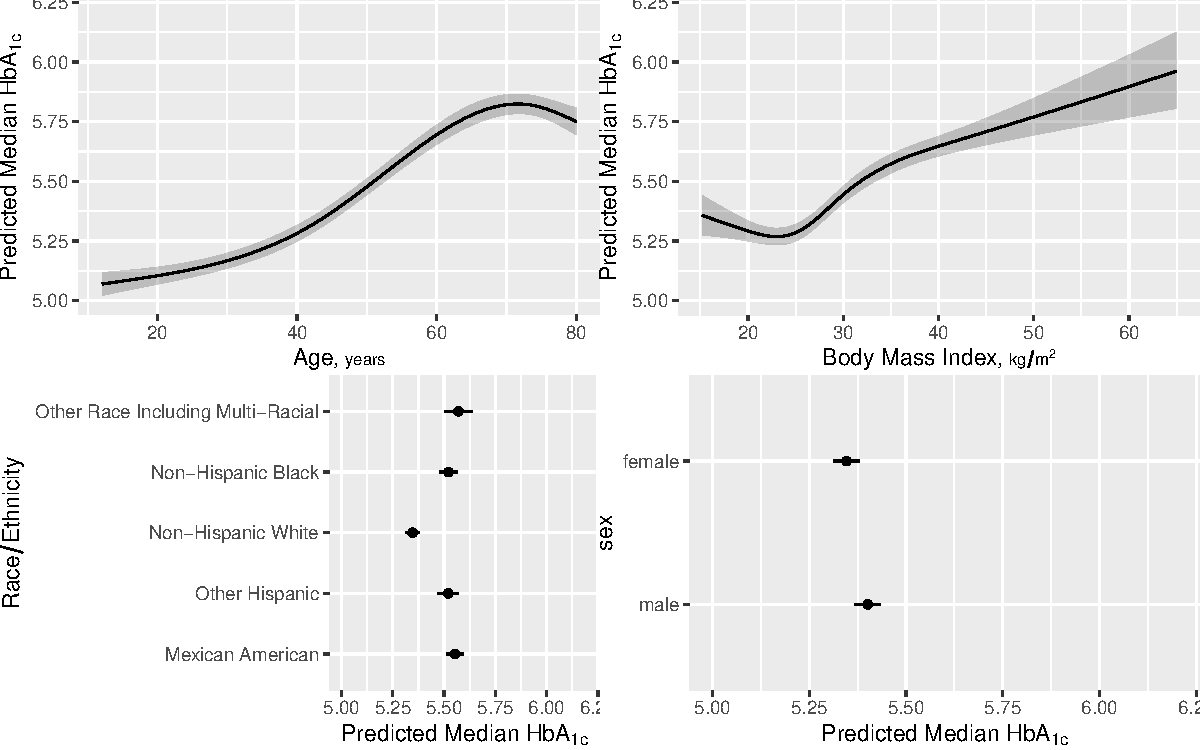
\includegraphics[width=\maxwidth]{descript-rmsa-1} }

\caption[Partial effects in NHANES HbA1c model]{Partial effects in NHANES HbA1c model}\label{fig:descript-rmsa}
\end{figure}

An effect chart is in Fig.~\ref{fig:descript-rmsb} and a nomogram is
in Fig.~\ref{fig:descript-rmsc}.  See
\url{http://stats.stackexchange.com/questions/155430/clarifications-regarding-reading-a-nomogram}
for excellent examples showing how to read such nomograms.
\begin{Schunk}
\begin{Sinput}
plot(summary(f))   # Fig. (*\ref{fig:descript-rmsb}*)
\end{Sinput}
\begin{figure}[htbp]

\centerline{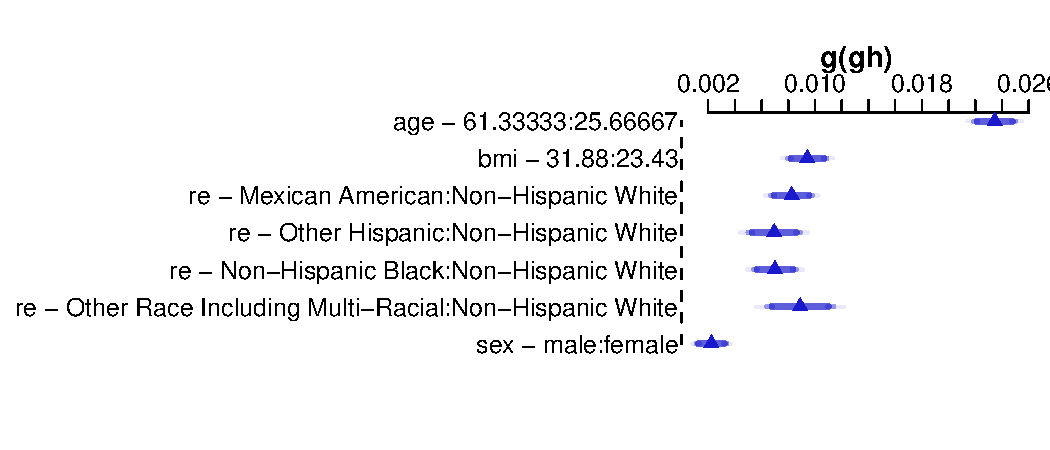
\includegraphics[width=\maxwidth]{descript-rmsb-1} }

\caption[Partial effects chart for transformed glycohemoglobin]{Partial effects chart on the transformed scale.  For age and BMI, effects are inter-quartile-range effects.  0.9, 0.95, and 0.99 confidence limits are shown.}\label{fig:descript-rmsb}
\end{figure}
\end{Schunk}
\begin{Schunk}
\begin{Sinput}
plot(nomogram(f, fun=ginverse, funlabel='Median HbA1c'))  # Fig. (*\ref{fig:descript-rmsc}*)
\end{Sinput}
\begin{figure}[htbp]

\centerline{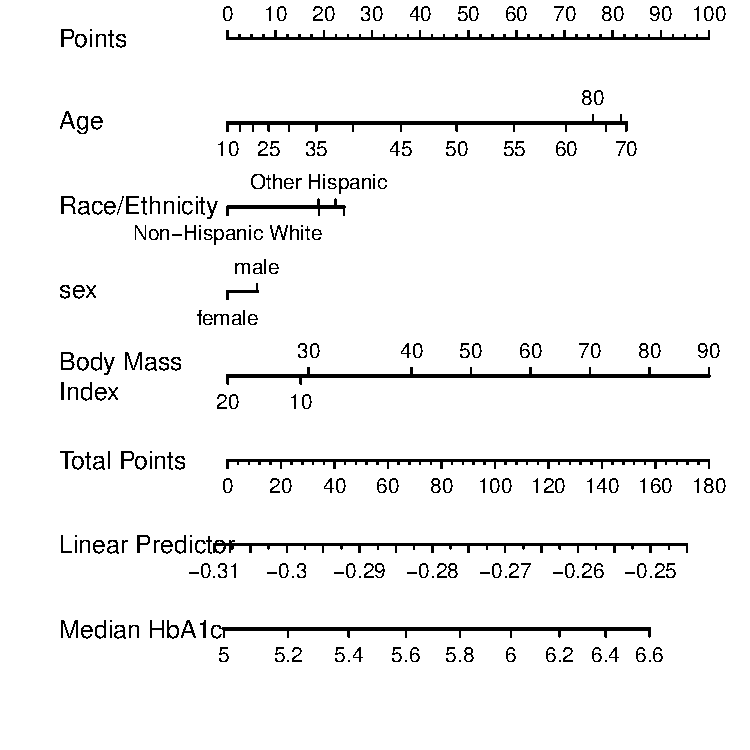
\includegraphics[width=\maxwidth]{descript-rmsc-1} }

\caption[Nomogram for predicting median HbA$_{1c}$]{Nomogram for predicting median HbA$_{1c}$.  To use the nomogram, use the top \Co{Points} scale to convert each predictor value to a common scale.  Add the points and read this number on the \Co{Total Points} scale, then read down to the median.}\label{fig:descript-rmsc}
\end{figure}
\end{Schunk}

\subsubsection{Graphing Effect of Two Continuous Variables on $Y$}
The following examples show the estimated combined effects of two
continuous predictors on outcome.  The two models included interaction
terms, the second example using penalized maximum likelihood
estimation with a tensor spline in diastolic $\times$ systolic blood pressure.

\begin{figure}[!htbp]\leavevmode%
 \centerline{\includegraphics[width=.9\textwidth]{image-sepsis}}
 \caption{Estimated median survival time for critically ill adults}
 \alabel{fig:descript-image-sepsis}
 \end{figure}

\begin{figure}[!htbp]\leavevmode%
 \centerline{\includegraphics[width=.9\textwidth]{image-stroke}}
 \caption[Probability of hemorrhagic stroke vs.\ blood
 pressures]{Logistic regression estimate of probability of a
   hemorrhagic stroke for patients in the GUSTO-I trial given $t$-PA,
   using a tensor spline of two restricted cubic splines and
   penalization (shrinkage).  Dark (cold color) regions are low risk,
   and bright (hot) regions are higher risk.}
 \alabel{fig:descript-image-stroke}
 \end{figure}
 
 Figure~\ref{fig:descript-image-stroke} is particularly interesting
 because the literature had suggested (based on approximately 24
 strokes) that pulse pressure was the main
 cause of hemorrhagic stroke whereas this flexible modeling approach
 (based on approximately 230 strokes)
 suggests that mean arterial blood pressure (roughly a $45^\circ$ line)
 is what is most important 
 over a broad range of blood pressures.  At the far right one can see
 that pulse pressure (axis perpendicular to $45^\circ$ line) may have
 an impact although a non-monotonic one.

\clearpage

\section{Tables} \bmovie{3a}\ddisc{3}
What are tables for?
\bi
\item Lookup of details
\item Not for seeing trends
\item For displaying a summary of a variable stratified by a truly
  categorical variable
\item Not for summarizing how a variable changes across levels of a
  continuous independent variable
\ei

Since tables are for lookup, they can be complex.  With modern media,
a better way to think of a table is as a pop-up when viewing elements
of a graph.

What to display in a table for different types of response variables:
\bi
\item Binary variables: Show proportions first; they should be
  featured because they are normalized for sample size
  \bi
  \item Don't need to show both proportions (e.g., only show
    proportion of females)
  \item Proportions are better than percents because of reduced
    confusion when speaking of percent difference (is it relative or
    absolute?) and because percentages such as 0.3\% are often
    mistaken for 30\% or 3\%.
  \ei
\item Make logical choices for independent and dependent variables. \\
 E.g., less useful to show proportion of males for patients who lived
 vs.\ those who died than to show proportion of deaths stratified by
 sex.
\item Continuous response variables
 \bi
 \item to summarize distributions of raw data: 3 quartiles \\
   recommended format: {\small 35} \textbf{50} {\small 67} or
   35/\textbf{50}/67
 \item summary statistics: mean or median and confidence limits
   (without assuming normality of data if possible)
 \ei
\item Continuous independent (baseline) variables
  \bi
  \item Don't use tables because these requires arbitrary binning
    (categorization) 
  \item Use graphs to show smooth relationships
  \ei
\item Show number of missing values
\item Add denominators when feasible
\item Confidence intervals: in a comparative study, show confidence
  intervals for differences, not confidence intervals for
  individual group summaries
\ei

\begin{table}[!h]
 \caption{Descriptive Statistics: Demographic and Clinical variables\label{summ1}}
 \begin{center}
 \begin{tabular}{lrc}\hline\hline
\multicolumn{1}{l}{}&
\multicolumn{1}{c}{N}&
\multicolumn{1}{c}{ }
\\ \hline
Age&27&{\scriptsize 28~}{\textbf{32} }{\scriptsize 52} \\
C-reactive~protein&27&{\scriptsize  1.0~}{ \textbf{1.8} }{\scriptsize 10.1} \\
Fecal~Calprotectin &26&{\scriptsize  128~}{ \textbf{754} }{\scriptsize 2500} \\
Gender&27&\\
~~~~Female&&0.52~{\scriptsize~$\frac{14}{27}$}\\
Location~of~colitis&27&\\
~~~~Left~side&&0.41~{\scriptsize~$\frac{11}{27}$}\\
~~~~Middle&&0.52~{\scriptsize~$\frac{14}{27}$}\\
~~~~Right~side&&0.07~{\scriptsize~$\frac{~2}{27}$}\\
\hline
\end{tabular}

\end{center}

\noindent {\scriptsize $a$\ }{$\mathbf{b}$\ }{\scriptsize $c$\ } represent the lower quartile $a$, the median $\mathbf{b}$, and the upper quartile $c$\ for continuous variables.\\
$N$\ is the number of non--missing values.\\

\end{table}

See also \href{https://hbiostat.org/talks/rmedicine19.html#18}{hbiostat.org/talks/rmedicine19.html\#18}.

%% Usage: knitr slide

\chapter{Hypothesis Testing}\abd{6}
\section{Overview}
Hypothesis testing using traditional frequentist statistical methods
often involves a ``straw man'' hypothesis in an 
attempt to placate reviewers who love $P$-values.  Estimation is more
often appropriate than hypothesis testing.  When hypothesis testing is
really necessary, a choice needs to be made between parametric
(usually Gaussian distribution-based) methods discussed in this
chapter and nonparametric methods to be covered in
Chapter~\ref{chap:nonpar}.  It is not appropriate to use a test of
normality to decide upon a course of action.  Such a strategy would
assume that
\be
\item the test for normality has power near 1.0 for all sample sizes
\item pre-testing for normality does not modify the type I error of
  the testing procedure
\item nonparametric tests are inefficient
\ee
In fact none of these assumptions is true.

We present parametric tests for the following reasons:
\be
\item historical
\item they are very useful for sample size estimation
\item occasionally one has prior information that the raw data, or
  differences from pre to post, actually follow a normal distribution,
  and with large effects one can get quite significant results in very
  small samples with parametric tests
\ee

\section{Hypotheses}
\subsection{Scientific Hypotheses and Questions}
Scientific questions are usually stated with a direction or with
regard to an expected effect, not with respect to a null effect.
Scientific questions often involve estimating a quantify of interest.
Here are some examples:
\bi
\item Does the risk of death increase when serum triglyceride
  increases?
\item Is mechanism $x$ responsible for regulation of physiologic
  parameter $y$?
\item What is the average decrease in blood pressure when the dose of
  a drug goes from 0 to 10mg/day to 20mg/day?
\ei
\subsection{Statistical Hypotheses}
\bi
\item Hypothesis: usually a statement to be judged of the form \\
  ``population value = specified constant''
 \bi
 \item $\mu = 120$mmHg
 \item $\mu_{1} - \mu_{2} = 0$mmHg
 \item Correlation between wealth and religiosity = 0
 \ei
\item Null hypothesis is usually a hypothesis of no effect but can be
 $H_{0}: \mu =$ constant or $H_{0}:$ Probability of heads
 $=\frac{1}{2}$; \\
 $H_{0}$ is often a straw man; something you hope to disprove
\item Alternative hypothesis: $H_1$; e.g.: $H_{1}: \mu \neq 120$mmHg
\item One-sided hypothesis (tested by 1-tailed test): $H_{1}$ is an
  inequality in one direction ($H_{1}: \mu > 120$mmHg)
\item Two-sided hypothesis (2-tailed test, most common type): $H_{1}$
  involves values far from the hypothesized value in either direction
\ei

\section{Branches of Statistics}
\bi
\item Classical (frequentist or sampling statistics)\ros{7.1-7.2}
 \bi
  \item Emphasizes (overemphasizes?) hypothesis testing
 \item Assumes $H_{0}$ is true and tries to amass evidence casting
   doubt on this assumption
 \item Conceives of data as one of many datasets that \emph{might} have
   happened; considers the process by which the sample arose
 \item Inference is based on long-run operating characteristics not
   about direct evidence from the sample at hand
   \bi
   \item false positive probability
   \item probability that varying confidence intervals over replicates
     of the experiment cover the true unknown parameter value a
     certain proportion of the time; no statement about whether the
     current confidence interval covers the true parameter or not
   \ei
 \item See if data are consistent with $H_{0}$
 \item Are data extreme or unlikely if $H_{0}$ is really true?
 \item Proof by contradiction: if assuming $H_{0}$ is true leads to
   results that are ``bizarre'' or unlikely to have been observed,
   casts doubt on premise
 \item Evidence summarized through a single statistic capturing a
   tendency of data, e.g., $\bar{x}$
 \item Look at probability of getting a statistic as or more extreme
   than the calculated one (results as or more impressive than ours)
   if $H_{0}$ is true (the $P$-value)
 \item If the statistic has a low probability of being observed to be
   this extreme we say
   that if $H_{0}$ is true we have acquired data that are very
   improbable, i.e., have witnessed a low probability event
 \item Then evidence mounts against $H_{0}$ and we might reject it
 \item A failure to reject \emph{does not} imply that we have gathered
   evidence in favor of $H_0$ --- many reasons for studies to not
   be impressive, including small sample size ($n$)
 \item Ignores \emph{clinical} significance
 \item Is fraught with how to deal with multiplicity problems
   \bi
   \item No principled recipe for how they should be handled
   \item Arise because
     \bi
     \item type I error is fixed at a number $> 0$
     \item backward time ordering of information
     \ei
   \item Evidence about one question is changed according to whether
     other questions are asked (regardless of their answers)
   \ei
 \ei
\item Classical parametric statistics: assumes the data to arise from
  a certain distribution, often the normal (Gaussian distribution)
\item Nonparametric statistics: does not assume a data distribution;
  generally looks at ranks rather than raw values
\item Bayesian statistics: \ros{7.8}
 \bi
 \item Considers the sample data, not how it arose
 \item Computes the probability that a clinically interesting
   statement is true, e.g. that the new drug lowers population mean
   SBP by at least 5mmHg, given what we observed in the data
 \item More natural and direct approach but requires more work
 \item Because respects forward flow of time/information there is no
   need for nor availability of methods for correcting for
   multiplicity\footnote{Bayesian inference assumes only that the
     prior distribution is ``well calibrated'' in the sense that one
     sticks to the pre-specified prior no matter what information is unveiled.}
 \item Evidence about one question is not tilted by whether other
   questions are asked
 \item Can formally incorporate knowledge from other studies as well
   as skepticism from a tough audience you are trying to convince to
   use a therapy
 \item Starting to catch on (only been available for about 240 years)
   and more software becoming available
 \ei
\item Likelihood inference:
  \bi
  \item Considers the sample data, not how it arose
  \item Akin to Bayesian but without the prior
  \item Interval estimates are based on relative likelihood (from the
    likelihood function) and are called likelihood support intervals
  \item For testing, allows both type I and type II errors
    $\rightarrow 0$ as $n \rightarrow \infty$, whereas with
    frequentist methods the type I error never shrinks as $n
    \rightarrow \infty$
  \item This greatly reduces problems with multiplicities
  \ei
\item Bayesian and likelihood inference use the \emph{likelihood
    principle}; frequentist inference does not 
 \bi
 \item Likelihood principle: All of the evidence in a sample relevant
   to model parameters is in the likelihood function 
 \item If we want to know our current location, frequentist inference
   asks the following: If I am in Nashville, what fraction of routes
   to here involved the southern route I took? 
   There are many paths to get where we are, and frequentists have to
   consider all possible relevant paths.  Bayesian and likelihood
   inference states it differently: Where am I now?  This involves an
   assessment of current evidence about my location.  Asking ``how did
   I get here?'' (i.e., how did the data arise?) involves multiplicity
   issues that answering the simpler question does not. 
\item Consider a sequentially monitored randomized experiment.
  Bayesians and likelihoodists can make infinitely many assessments of
  efficacy with no penalty.  On the other hand, a frequentist must
  think the following way:
  \begin{quote}
    I am at the first interim analysis.  I am going to make later
    assessments of efficacy so I need to discount the current
    assessment and be more conservative or I will spend all my
    $\alpha$ already.\\
    \ldots\\
    I am at the fifth interim analysis.  I made four previous efficacy
    assessments, and even though none of them mattered, I spent
    $\alpha$ so I need to discount the current assessment and be more
    conservative.
 \end{quote}
 \ei
\item We will deal with classical parametric and nonparametric
  statistical tests because of time and because software has evolved further
\ei

\section{Errors in Hypothesis Testing; $P$ Values} \ros{7.2}\katz{7.5.A-7.5.B}
\bi
\item Can attempt to reject a formal hypothesis or just compute
  $P$-value
\item Type I error: rejecting $H_0$ when it is true \\
  $\alpha$ is the probability of making this error (typically set at
  $\alpha=0.05$---for weak reasons)
\item Type II error: failing to reject $H_0$ when it is false \\
  probability of this is $\beta$
\begin{center}
\begin{tabular}{|l||c|c|} \hline
 & \multicolumn{2}{|c|}{True state of $H_0$} \\ \hline 
Decision & $H_0$ true & $H_0$ false \\ \hline \hline
Reject $H_0$ & Type I error ($\alpha$) & Correct \\  \hline
Do Not Reject $H_0$ & Correct & Type II error ($\beta$) \\  \hline
\end{tabular}
\end{center}

\item Power: $1 - \beta$: probability of (correctly) rejecting $H_0$
  when it is false
\ei

Within the frequentist framework of statistics there are two schools.
One, the Neyman-Pearson school, believes that the type I error should
be pre-set at $\alpha$ (say $\alpha=0.05$) so that binary decisions
can be made (reject/fail to reject).  The other school due to Fisher
believes that one should compute $P$-values and quote the result in
the report or publication.  This is the more popular approach, for
good reason.

A $P$-value is something that can be computed without speaking of
errors.  It is the probability of observing a statistic as or more
extreme than the observed one if $H_0$ is true, i.e., if the
population from which the sample was randomly chosen had the
characteristics posited in the null hypothesis.\footnote{Note that
  Rosner's Equation 7.4 in his section 7.3 is highly 
problematic.  Classifications of ``significant'' or ``highly
significant'' are arbitrary, and treating a $P$-value between 0.05 and
0.1 as indicating a ``trend towards significance'' is bogus.  If the
$P$-value is 0.08, for example, the 0.95 confidence interval for the
effect includes a ``trend'' in the opposite (harmful) direction.}

\subsection{Misinterpretation of $P$-values}
$P$-values have come under extreme criticism since 2000, partially
because they are often misinterpreted. Greenland~\etal~\cite{gre16sta}
is the best paper that summarizes the misinterpretations and explains
them.  Some quotes from this paper are below, with their explanations
for the first two.

\begin{quote}
  \begin{enumerate}
  \item \textbf{The $P$ value is the probability that the test
      hypothesis is true; for example, if a test of the null
      hypothesis gave $P$ = 0.01, the null hypothesis has only a 1\%
      chance of being true; if instead it gave $P$ = 0.40, the null
      hypothesis has a 40\% chance of being true.} No! The $P$ value
    assumes the test hypothesis is true---it is not a hypothesis
    probability and may be far from any reasonable probability for the
    test hypothesis. The $P$ value simply indicates the degree to
    which the data conform to the pattern predicted by the test
    hypothesis and all the other assumptions used in the test (the
    underlying statistical model). Thus $P$ = 0.01 would indicate that
    the data are not very close to what the statistical model
    (including the test hypothesis) predicted they should be, while
    $P$ = 0.40 would indicate that the data are much closer to the
    model prediction, allowing for chance variation. 
  \item \textbf{The $P$ value for the null hypothesis is the
      probability that chance alone produced the observed association;
      for example, if the $P$ value for the null hypothesis is 0.08,
      there is an 8\% probability that chance alone produced the
      association.}  No! This is a common variation of the first
    fallacy and it is just as false. To say that chance alone produced
    the observed association is logically equivalent to asserting that
    every assumption used to compute the $P$ value is correct, including
    the null hypothesis. Thus to claim that the null $P$ value is the
    probability that chance alone produced the observed association is
    completely backwards: The $P$ value is a probability computed
    assuming chance was operating alone. The absurdity of the common
    backwards interpretation might be appreciated by pondering how
    the $P$ value, which is a probability deduced from a set of
    assumptions (the statistical model), can possibly refer to the
    probability of those assumptions. Note: One often sees ``alone''
    dropped from this description (becoming ``the $P$ value for the null
    hypothesis is the probability that chance produced the observed
    association''), so that the statement is more ambiguous, but just
    as wrong.
  \item \textbf{A significant test results ($P\leq 0.05$) means that
      the test hypothesis is false or should be rejected.} No!
  \item \textbf{A nonsignificant test results ($P > 0.05$) means that
      the test hypothesis is true or should be accepted.} No!
  \item \textbf{A large $P$ value is evidence in favor of the test
      hypothesis.} No!
  \item \textbf{A null-hypothesis $P$ value greater than 0.05 means
      that no effect was observed, or that absence of an effect was
      shown or demonstrated.} No!
  \item \textbf{Statistical significance indicates a scientifically or
      substantively important relation has been detected.} No!
  \item \textbf{Lack of statistical significance indicates that the
      effect size is small.} No!
  \item \textbf{The $P$ value is the chance of our data occurring if
      the test hypothesis is true; for example, $P$ = 0.05 means that
      the observed association would occur only 5\% of the time under
      the test hypothesis.} No!
  \item \textbf{If you reject the test hypothesis because $P \leq
      0.05$, the change you are in error (the chance your
      ``significant finding'' is a false positive) is 5\%.} No!
  \item \textbf{$P = 0.05$ and $P \leq 0.05$ mean the same thing.} No!
  \item \textbf{$P$ values are properly reported as inequalities (e.g., report ``$P < 0.02$'' when $P = 0.015$ or report $P > 0.05$ when $P = 0.06$ or $P = 0.70$).} No!
  \item \textbf{Statistical significance is a property of the phenomenon being studied, and thus statistical tests detect significance.} No!
  \item \textbf{One should always use two-sided $P$ values.} No!
  \item \textbf{When the same hypothesis is tested in different studies and none or a minority of the tests are statistically significant (all $P > 0.05$), the overall evidence supports the hypothesis.} No!
  \item \textbf{When the same hypothesis is tested in two different populations and the resulting $P$ values are on opposite sides of 0.05, the results are conflicting.} No!
  \item \textbf{When the same hypothesis is tested in two different populations and the same $P$ values are obtained, the results are in agreement.} No!
  \item \textbf{If one observes a small $P$ value, there is a good chance that the next study will produce a $P$ value at least as small for the same hypothesis.} No!
  \item \textbf{The specific 95\% confidence interval presented by a study has a 95\% chance of containing the true effect size.} No!
  \item \textbf{An effect size outside the 95\% confidence interval has been refuted (or excluded) by the data.} No!
  \item \textbf{If two confidence intervals overlap, the difference between the two estimates or studies is not significant.} No!
  \item \textbf{An observed 95\% confidence interval predicts that 95\% of the estimates from future studies will fall inside the observed interval.} No!
  \item \textbf{If one 95\% confidence interval includes the null value and another excludes that value, the interval excluding the null is the more precise one.} No!
  \item \textbf{If you accept the null hypothesis because the null $P$ value exceeds 0.05 and the power of your test is 90\%, the chance you are in error (the chance that your finding is a false negative) is 10\%.} No!
  \item \textbf{If the null $P$ value exceeds 0.05 and the power of this test is 90\% at an alternative, the results support the null over the alternative.} \dots counterexamples are easy to construct \dots
 \end{enumerate}
\end{quote}

\section{One Sample Test for Mean} \ros{7.3-7.4,7.12}
\subsection{Test}
\bi
\item Assuming continuous response from a normal distribution
\item One sample tests for $\mu =$ constant are unusual except when
  data are paired, e.g., each patient has a pre-- and post--treatment
  measurement and we are only interested in the mean of post - pre
  values
\item $t$ tests in general:
\beq
t = \frac{\textrm{estimate - hypothesized value}}{\textrm{standard deviation
  of numerator}}
\eeq
\item The standard deviation of a summary statistic is called its
  \emph{standard error}, which is the $\sqrt{}$ of the variance of the
  statistic 
\item The one-sample $t$ statistic for testing a single population
  mean against a constant $\mu_0$ ($H_{0}$: $\mu = \mu_{0}$; often
  $\mu_{0} = 0$) is 
\beq
t = \frac{\bar{x} - \mu_{0}}{se}
\eeq
where $se = \frac{s}{\sqrt{n}}$, is the standard error of the mean (SEM) and $\bar{x}$ is the sample mean

%because the variance of $\bar{x}$ is the variance of an individual $x$ value divided by the number of values being averaged $\rightarrow \sigma^{2}/n$
% \bi
% \item If you repeated an experiment $M$ times, each time computing
%   $\bar{x}$ from $n$ observations, the $M \bar{x}$s would vary
%   $\frac{1}{n}$th as much as the raw measurements vary between
%   patients
% \ei
\item When your data comes from a normal distribution and $H_{0}$ holds, the
  $t$ ratio follows the $t$ \emph{distribution}
\item With small sample size ($n$), the $t$ ratio is unstable because the sample standard deviation ($s$) is not
  precise enough in estimating the population standard deviation ($\sigma$; we are assuming that $\sigma$
  is unknown)
\item This causes the $t$ distribution to have heavy tails for small
  $n$
\item As $n\uparrow$ the $t$ distribution becomes the normal
  distribution with mean zero and standard deviation one
\item The parameter that defines the particular $t$ distribution to
  use as a function of $n$ is called the \emph{degrees of freedom} or
  d.f.
\item d.f. = $n$ - number of means being estimated
\item For one-sample problem d.f. = $n-1$
\item Symbol for distribution $t_{n-1}$

\begin{Schunk}
\begin{Sinput}
x <- seq(-3, 3, length=200)   # Fig. (*\ref{fig:htest-tpdfs}*)
w <- list(Normal     = list(x=x, y=dnorm(x)),
          't (50 df)'= list(x=x, y=dt(x, 50)),
          't (5 df)' = list(x=x, y=dt(x, 5)),
          't (2 df)' = list(x=x, y=dt(x,2)))
require(Hmisc)
labcurve(w, pl=TRUE, keys='lines', col=c(1,2,4,5), lty=c(2,1,1,1),
         xlab=expression(x), ylab='')
\end{Sinput}
\begin{figure}[htbp]

\centerline{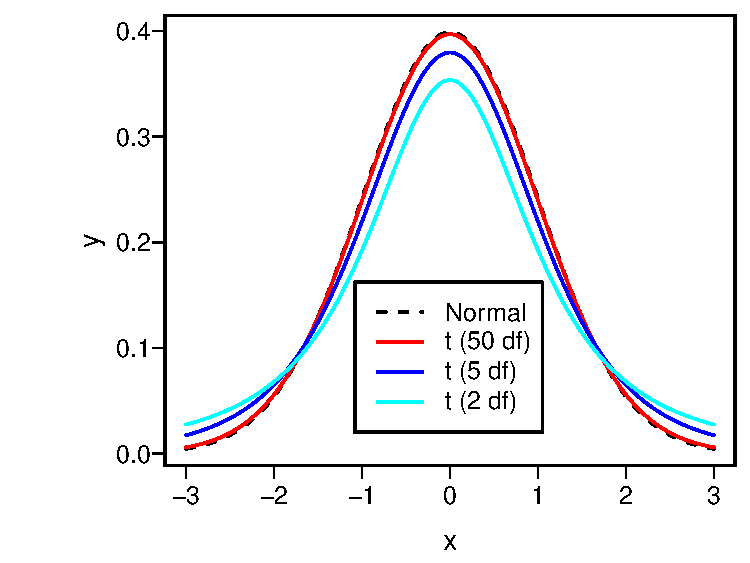
\includegraphics[width=\maxwidth]{htest-tpdfs-1} }

\caption[$t$ distribution for varying d.f.]{Comparison of probability densities for $t_2$, $t_5$, $t_{50}$, and normal distributions}\label{fig:htest-tpdfs}
\end{figure}
\end{Schunk}

\item Two-tailed $P$-value: probability of getting a value from the
  $t_{n-1}$ distribution as big or bigger in absolute value than the
  absolute value of the observed $t$ ratio
\item Computer programs can compute the $P$-value given $t$ and
  $n$.\footnote{\R\ has the function \texttt{pt} for the cumulative
    distribution function for the $t$ distribution, so the 2-tailed
    $P$-value would be obtained using 
    \texttt{2*(1-pt(abs(t),n-1))}.}  See the course web site or go
  to \url{http://surfstat.anu.edu.au/surfstat-home/tables/t.php} for
  an interactive $P$ and critical value calculator for common
  distributions.  But \R\ can compute all probabilities or critical
  values of interest.  See the help files for \co{pt,pnorm,pf,pchisq}.
 \bi
 \item don't say ``$P <$ something'' but instead $P=$ something
 \ei
\item In the old days tables were used to provide \emph{critical
    values} of $t$, i.e., a value $c$ of $t$ such that Prob$[|t| > c]
  = \alpha$ for ``nice'' $\alpha$ such as 0.05, 0.01.
\item Denote the critical value by $t_{n-1;1-\alpha/2}$ for a 2-tailed setup
\item For large $n$ (say $n \geq 500$) and $\alpha=0.05$, this value approximates
  the value from the normal distribution, 1.96
\item Example:  We want to test if the mean tumor volume is 190 mm$^3$ in a population with melanoma, $H_0: \mu = 190$ versus $H_1: \mu \neq 190$.
\beqa
\bar{x}=181.52, s=40, n=100, \mu_{0}=190 \\
t = \frac{181.52 - 190}{40/\sqrt{100}} = -2.12 \\
t_{99,.975}=1.984 \rightarrow \mathrm{reject~at~\alpha=.05} \\
P=0.037
\eeqa
\ei
\begin{Schunk}
\begin{Sinput}
xbar  <- 181.52
s     <- 40
n     <- 100
mu0   <- 190
tstat <- (xbar - mu0) / (s / sqrt(n))
pval  <- 2 * (1 - pt(abs(tstat), n - 1))
c(tstat=tstat, pval=pval)
\end{Sinput}
\begin{Soutput}
      tstat        pval 
-2.12000000  0.03650607 
\end{Soutput}
\end{Schunk}

\subsection{Power and Sample Size} \ros{7.5-7.6}
\bi
\item Power $\uparrow$ when
 \bi
 \item allow larger type I error ($\alpha$; trade-off between type I
   and II errors)
 \item true $\mu$ is far from $\mu_{0}$
 \item $\sigma \downarrow$
 \item $n \uparrow$
 \ei
\item Power for 2-tailed test is a function of $\mu, \mu_{0}$ and
  $\sigma$ only through  $|\mu - \mu_{0}| / \sigma$
\item Sample size to achieve $\alpha=0.05$, power $=0.9$ is approximately
\beq
n = 10.51 \left[\frac{\sigma}{\mu-\mu_{0}}\right]^{2}
\eeq
\item Some power calculators are at \url{statpages.org/#Power}
\item Better: PS program by Dupont and Plummer \url{http://biostat.mc.vanderbilt.edu/PowerSampleSize}

\item Example: The mean forced expiratory volume (FEV) in a population of asthmatics is 2.5 liters per second and the population standard deviation is assumed to be 1.  Determine the number of subjects needed if a new drug is expected to increase FEV to 3.0 liters per second ($\alpha = .05, \beta = 0.1$)
\beqa
\mu=2.5, \mu_0=3, \sigma = 1 \\
n = 10.51 \left[\frac{1}{3-2.5}\right]^{2} = 42.04
\eeqa
  \bi
  \item \textrm{Rounding up, we need 43 subjects to have 0.9 power (42 subjects would have less than 0.9 power)}
  \ei
\ei
\begin{Schunk}
\begin{Sinput}
sigma <- 1
mu    <- 2.5
mu0   <- 3
n     <- 10.51 * (1 / (mu - mu0)) ^ 2
# General formula for approximate power of 1-sample t-test
# Approximate because it uses the normal distribution throughout,
# not the t distribution
alpha <- 0.05
power <- 0.9
delta <- mu - mu0
za    <- qnorm(1 - alpha / 2)
zb    <- qnorm(power)
n     <- ((za + zb) * sigma / delta) ^ 2
c(alpha=alpha, power=power, delta=delta, za=za, zb=zb, n=n)
\end{Sinput}
\begin{Soutput}
    alpha     power     delta        za        zb         n 
 0.050000  0.900000 -0.500000  1.959964  1.281552 42.029692 
\end{Soutput}
\end{Schunk}
A slightly more accurate estimate can be obtained using the $t$
distribution, requiring iterative calculations programmed in \R\
packages such as \co{pwr}.
\begin{Schunk}
\begin{Sinput}
# Make sure pwr package is installed
require(pwr)
\end{Sinput}
\begin{Sinput}
pwr.t.test(d = delta / sigma, power = 0.9, sig.level = 0.05, type='one.sample')
\end{Sinput}
\begin{Soutput}

     One-sample t test power calculation 

              n = 43.99548
              d = 0.5
      sig.level = 0.05
          power = 0.9
    alternative = two.sided
\end{Soutput}
\end{Schunk}

\subsection{Confidence Interval} \ros{R7.7}\altman{28-29}\abd{6.6}
A 2-sided $1-\alpha$ confidence interval for $\mu$ is
\beq
\bar{x} \pm t_{n-1,1-\alpha/2} \times {se}
\eeq
The $t$ constant is the $1-\alpha/2$ level critical value from the
$t$-distribution with $n-1$ degrees of freedom.  For large $n$ it
equals 1.96 when $\alpha=0.05$.

A rough way to interpret this is that we are 0.95 confident that the
unknown $\mu$ lies in the above interval.  The exact way to say it is
that if we were able to repeat the same experiment 1000 times and
compute a fresh confidence interval for $\mu$ from each sample, we
expect 950 of the samples to actually contain $\mu$.  The confidence
level is about the procedure used to derive the interval, not about
any one interval.  Difficulties in
providing exact interpretations of confidence intervals has driven
many people to Bayesian statistics.

The 2-sided $1-\alpha$ CL includes $\mu_{0}$ if and only if a test of $H_{0}:
\mu=\mu_{0}$ is not rejected at the $\alpha$ level in a 2-tailed test.
\bi
\item If a 0.95 CL does not contain zero, we can reject $H_0: \mu = 0$ at the $\alpha = 0.05$ significance level
\ei

$1 - \alpha$ is called the \emph{confidence level} or \emph{confidence
  coefficient}.

\subsection{Sample Size for a Given Precision} \altman{139-148}\abd{14.7}
There are many reasons for preferring to run estimation studies
instead of hypothesis testing studies.  A null hypothesis may be
irrelevant, and when there is adequate precision one can learn from a
study regardless of the magnitude of a $P$-value.  A universal
property of precision estimates is that, all other things being equal,
increasing the sample size by a factor of four improves the precision
by a factor of two.
\bi
\item May want to estimate $\mu$ to within a margin of error of $\pm
  \delta$ with 0.95 confidence\footnote{Adcock~\cite{adc97sam}
    presents both frequentist and Bayesian methods and for precision
    emphasizes solving for $n$ such that the probability of being
    within $\epsilon$ of the true value is controlled, as opposed to
    using confidence interval widths explicitly.}
\item ``0.95 confident'' that a confidence interval includes the true
  value of $\mu$
\item If $\sigma$ were known but we still used the $t$ distribution in
  the formula for the interval, the confidence interval would be
  $\bar{x}\pm \delta$ where
\beq
\delta = \frac{t_{n-1,1-\alpha/2}\sigma}{\sqrt{n}}
\eeq
\item Solving for $n$ we get
\beq
n = \left[\frac{t_{n-1,1-\alpha/2} \sigma}{\delta}\right]^{2}
\eeq
\item If $n$ is large enough and $\alpha=0.05$, required
  $n=3.84[\frac{\sigma}{\delta}]^{2}$
\item Example: if want to be able to nail down $\mu$ to within $\pm
  1$mmHg when the patient to patient standard deviation in blood
  pressure is 10mmHg, $n = 384$
\begin{Schunk}
\begin{Sinput}
sigma <- 10
delta <- 1
3.84 * (sigma / delta) ^ 2
\end{Sinput}
\begin{Soutput}
[1] 384
\end{Soutput}
\end{Schunk}
\item Advantages of planning for precision rather than
  power\footnote{See Borenstein M: \emph{J Clin Epi} 1994;
    47:1277-1285.}
 \bi
 \item do not need to guess the true population value
 \item many studies are powered to detect a miracle and nothing less;
   if a miracle doesn't happen, the study provides \textbf{no} information
 \item planning on the basis of precision will allow the resulting
   study to be interpreted if the $P$-value is 
   large, because the confidence interval will not be so wide as to
   include both clinically significant improvement and clinically
   significant worsening
 \ei
\ei

\section{One Sample Method for a Probability} \ros{7.10}\altman{45-56}\abd{7}
\subsection{Test}
\bi
\item Estimate a population probability $p$ with a sample probability
  $\hat{p}$
\item Approximate 2-sided test of $H_{0}: p=p_{0}$ obtained by
  computing a $z$ statistic
\item A $z$-test is a test assuming that the \emph{test statistic} has
  a normal distribution; it is a $t$-test with infinite ($\infty$) d.f.
\beq
z = \frac{\hat{p} - p_{0}}{\sqrt{p_{0}(1-p_{0})/n}}
\eeq
\item The $z$-test follows the same general form as the $t$-test
\beq
z = \frac{\textrm{estimate - hypothesized value}}{\textrm{standard deviation
  of numerator}}
\eeq
\item Example: $n=10$ tosses of a coin, 8 heads; $H_{0}$: coin is fair
  ($p_{0}=\frac{1}{2}$)
\beq
z = \frac{.8 - .5}{\sqrt{(\frac{1}{2})(\frac{1}{2})/10}} = 1.897
\eeq
\item $P\textrm{-value} = 2 \times$ area under a normal curve to the right of $1.897 =
  2 \times 0.0289 = 0.058$ (this is also the area under the normal
  curve to the right of $1.897$ + the area to the left of $-1.897$)
\begin{Schunk}
\begin{Sinput}
p  <- 0.8
p0 <- 0.5
n  <- 10
z  <- (p - p0) / sqrt(p0 * (1 - p0) / n)
c(z=z, Pvalue=2 * pnorm(-abs(z)))
\end{Sinput}
\begin{Soutput}
         z     Pvalue 
1.89736660 0.05777957 
\end{Soutput}
\end{Schunk}
\item Approximate probability of getting 8 or more or 2 or fewer heads
  if the coin is fair is 0.058
\item Need to use exact methods if $p$ or $n$ is small
\begin{Schunk}
\begin{Sinput}
# Pr(X >= 8) = 1 - Pr(X < 8) = 1 - Pr(X <= 7)
pbinom(2, 10, 0.5) + 1 - pbinom(7, 10, 0.5)
\end{Sinput}
\begin{Soutput}
[1] 0.109375
\end{Soutput}
\begin{Sinput}
# Also compute as the probability of getting 0, 1, 2, 8, 9, 10 heads
sum(dbinom(c(0, 1, 2, 8, 9, 10), 10, 0.5))
\end{Sinput}
\begin{Soutput}
[1] 0.109375
\end{Soutput}
\end{Schunk}
\ei

\subsection{Power and Sample Size}
\bi
\item Power $\uparrow$ as $n \uparrow$, $p$ departs from $p_{0}$, or
  $p_{0}$ departs from $\frac{1}{2}$
\item $n \downarrow$ as required power $\downarrow$ or $p$ departs
  from $p_{0}$
\ei

\subsection{Sample Size for Given Precision}\alabel{sec:htest-p-n}
\bi
\item Approximate 0.95 CL: $\hat{p} \pm 1.96
  \sqrt{\hat{p}(1-\hat{p})/n}$
\item Assuming $p$ is between 0.3 and 0.8, it would not be far off to
  use the worst case standard error $\sqrt{1/(4n)}$ when planning
\item $n$ to achieve a margin of error $\delta$ in estimating $p$: 
\beq
n = \frac{1}{4}\left[\frac{1.96}{\delta}\right]^{2} = \frac{0.96}{\delta^{2}}
\eeq
\item Example: $\delta=.1 \rightarrow n=96$ to achieve a margin of error of
  $\pm 0.1$ with 0.95 confidence
\ei
\begin{Schunk}
\begin{Sinput}
nprec <- function(delta) round(0.25 * (qnorm(0.975) / delta) ^ 2)
nprec(0.1)
\end{Sinput}
\begin{Soutput}
[1] 96
\end{Soutput}
\end{Schunk}

To achive a margin of error of $\pm 0.05$ even in the worst case where
$p=0.5$ one needs $n=384$.

To put this in the context of relative errors, suppose that one wants
to estimate the odds that an event will occur, to within a certain
multiplicative margin of error (MMOE) with 0.95 confidence.  What is
the MMOE as a function of the unknown $p$ when $n=384$?  The standard
error of the log odds is approximately $\sqrt{\frac{1}{n p (1 - p)}}$,
and the half-width of a 0.95 confidence interval for the log odds is
approximately 1.96 times that.  Fix $n=384$ and vary $p$ to get the
MMOE that is associated with the same sample size as a universal
absolute margin of error of 0.05.

\begin{Schunk}
\begin{Sinput}
p <- seq(0.01, 0.99, length=200)
mmoe <- exp(1.96 / sqrt(384 * p * (1 - p)))
plot(p, mmoe, type='l', xlab='Unknown Probability p', ylab='MMOE')
minor.tick()
\end{Sinput}
\begin{figure}[htbp]

\centerline{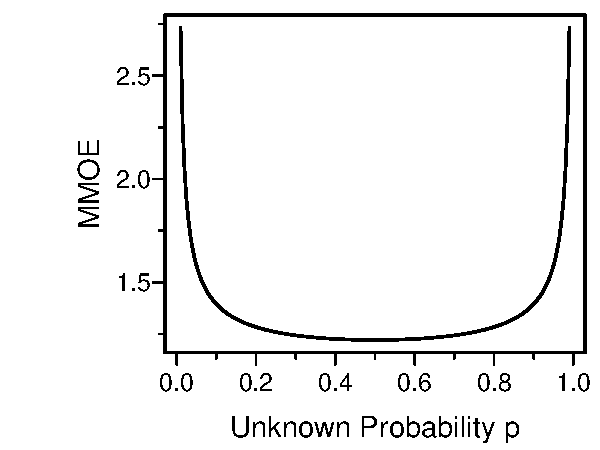
\includegraphics[width=\maxwidth]{htest-moeor-1} }

\caption[Multiplicative margin of error in estimating odds when $n=384$ and the margin of error in estimating the absolute probability is $\leq 0.05$]{Multiplicative margin of error in estimating odds when $n=384$ and the margin of error in estimating the absolute probability is $\leq 0.05$.}\label{fig:htest-moeor}
\end{figure}
\end{Schunk}

\section{Paired Data and One-Sample Tests}  \altman{31-32}\abd{11}
\bi
\item To investigate the relationship between smoking and bone mineral
  density, Rosner presented a paired analysis in which each person had
  a nearly perfect control which was his or her twin
\item Data were normalized by dividing differences by the mean density
  in the twin pair (need to check if this normalization worked)
\item Computed density in heavier smoking twin minus density in
  lighter smoking one
\item Mean difference was $-5\%$ with se=$2.0\%$ on $n=41$
\item The $t$ statistic we've been using works here, once within-pair
  differences are formed
\item $H_{0}:$ mean difference between twins is zero ($\mu_{0} = 0$)
\beqa
t_{40} = \frac{\bar{x} - \mu_{0}}{se} = -2.5 \\
P = 0.0166
\eeqa
\ei
\begin{Schunk}
\begin{Sinput}
xbar  <- -5
se    <- 2
n     <- 41
mu0   <- 0
tstat <- (xbar - mu0) /se
pval  <- 2 * (1 - pt(abs(tstat), n - 1))
c(tstat=tstat, Pvalue=pval)
\end{Sinput}
\begin{Soutput}
      tstat      Pvalue 
-2.50000000  0.01662035 
\end{Soutput}
\end{Schunk}

\section{Two Sample Test for Means} \ros{8}\katz{5.5}\altman{28-35}\abd{12}
\bi
\item Two groups of different patients (unpaired data)
\item Much more common than one-sample tests
\item As before we are dealing for now with parametric tests assuming
  the raw data arise from a normal distribution
\item We assume that the two groups have the same
  spread or variability in the distributions of
  responses\footnote{Rosner covers the unequal variance case very
    well.  As nonparametric tests have advantages for comparing two
    groups and are less sensitive to the equal spread assumption, we
    will not cover the unequal variance case here.}
\ei

\subsection{Test}
\bi
\item Test whether population 1 has the same mean as population 2
\item Example: pop.\ 1=all patients with a certain disease if given
  the new drug, pop.\ 2=standard drug
\item $H_{0}: \mu_{1}=\mu_{2}$ (this can be generalized to test
  $\mu_{1}=\mu_{2}+\delta$, i.e., $\mu_{1}-\mu_{2}=\delta$).  The
  \emph{quantity of interest} or \emph{QOI} is $\mu_{1}-\mu_{2}$
\item 2 samples, of sizes $n_{1}$ and $n_{2}$ from two populations
\item Two-sample (unpaired) $t$-test assuming normality and equal
variances---recall that if we are testing against an $H_0$ of
\textbf{no effect}, the form of the $t$ test is
\beq
t =
\frac{\mathrm{point~estimate~of~QOI}}{\mathrm{se~of~numerator}}
\eeq
\item Point estimate QOI is $\bar{x}_{1} - \bar{x}_{2}$
\item Variance of the sum or difference of two independent means is
  the sum of the variance of the individual means
\item This is $\frac{\sigma^{2}}{n_{1}} + \frac{\sigma^{2}}{n_{2}} =
  \sigma^{2}[\frac{1}{n_{1}} + \frac{1}{n_{2}}]$
\item Need to estimate the single $\sigma^{2}$ from the two samples
\item We use a weighted average of the two sample variances:
\beq
s^{2} = \frac{(n_{1}-1)s^{2}_{1} + (n_{2}-1)s^{2}_{2}}{n_{1}+n_{2}-2}
\eeq
\item True standard error of the difference in sample means: $\sigma
  \sqrt{\frac{1}{n_{1}} + \frac{1}{n_{2}}}$
\item Estimate: $s \sqrt{\frac{1}{n_{1}} + \frac{1}{n_{2}}}$, so
\beq
t = \frac{\bar{x}_{1} - \bar{x}_{2}}{s \sqrt{\frac{1}{n_{1}} + \frac{1}{n_{2}}}}
\eeq
\item d.f.\ is the sum of the individual d.f., $n_{1}+n_{2}-2$, where
  the $-2$ is from our having to estimate the center of two
  distributions
\item If $H_{0}$ is true $t$ has the $t_{n_{1}+n_{2}-2}$ distribution
\item To get a 2-tailed $P$-value we compute the probability that a
  value from such a distribution is farther out in the tails of the
  distribution than the observed $t$ value is (we ignore the sign of
  $t$ for a 2-tailed test)
\item Example: $n_{1}=8, n_{2}=21, s_{1}=15.34, s_{2}=18.23,
  \bar{x}_{1}=132.86, \bar{x}_{2}=127.44$
\beqa
s^{2} &=& \frac{7(15.34)^{2}+20(18.23)^{2}}{7+20} = 307.18 \\
s     &=& \sqrt{307.18} = 17.527 \\
se    &=& 17.527 \sqrt{\frac{1}{8}+\frac{1}{21}} = 7.282 \\
t     &=& \frac{5.42}{7.282} = 0.74
\eeqa
on 27 d.f.
\item $P = 0.463$ (see \R\ code below)
\item Chance of getting a difference in means as larger or larger than
  5.42 if the two populations really have the same means is 0.463
\item $\rightarrow$ little evidence for concluding the population
  means are different
\ei
\begin{Schunk}
\begin{Sinput}
n1    <- 8;         n2 <- 21
xbar1 <- 132.86; xbar2 <- 127.44
s1    <- 15.34;     s2 <- 18.23
s     <- sqrt(((n1 - 1) * s1 ^ 2 + (n2 - 1) * s2 ^ 2) / (n1 + n2 - 2))
se    <- s * sqrt(1 / n1 + 1 / n2)
tstat <- (xbar1 - xbar2) / se
pval  <- 2 * (pt(- abs(tstat), n1 + n2 - 2))
c(s=s, se=se, tstat=tstat, Pvalue=pval)
\end{Sinput}
\begin{Soutput}
         s         se      tstat     Pvalue 
17.5265589  7.2818380  0.7443176  0.4631137 
\end{Soutput}
\end{Schunk}

\subsection{Power and Sample Size}
\bi
\item Power increases when
 \bi
 \item $\Delta = |\mu_{1}-\mu_{2}| \uparrow$
 \item $n_{1} \uparrow$ or $n_{2} \uparrow$
 \item $n_{1}$ and $n_{2}$ are close
 \item $\sigma \downarrow$
 \item $\alpha \uparrow$
 \ei
\item Power depends on $n_{1}, n_{2}, \mu_{1}, \mu_{2}, \sigma$
  approximately through 
\beq
\frac{\Delta}{\sigma \sqrt{\frac{1}{n_{1}}+\frac{1}{n_{2}}}}
\eeq
\item Note that when computing power using a program that asks for
  $\mu_{1}$ and $\mu_{2}$ you can just enter 0 for $\mu_{1}$ and enter
  $\Delta$ for $\mu_{2}$, as only the difference matters
\item Often we estimate $\sigma$ from pilot data, and to be honest we
  should make adjustments for having to estimate $\sigma$ although we
  usually run out of gas at this point
\item Use the \R\ \co{pwr} package, or the power calculator at
  \url{statpages.org/#Power} or PS 
\item Example: \\
 Get a pooled estimate of $\sigma$ using $s$ above (17.52656) \\
% $\sqrt{\frac{15.34^{2}+18.23^{2}}{2}} = 
% 16.847$ when
 Use $\Delta=5, n_{1}=n_{2}=100, \alpha=0.05$
\begin{Schunk}
\begin{Sinput}
delta <- 5
require(pwr)
pwr.t2n.test(n1=100, n2=100, d=delta / s, sig.level = 0.05)
\end{Sinput}
\begin{Soutput}

     t test power calculation 

             n1 = 100
             n2 = 100
              d = 0.2852813
      sig.level = 0.05
          power = 0.5189751
    alternative = two.sided
\end{Soutput}
\end{Schunk}
\item Sample size depends on $k = \frac{n_{2}}{n_{1}}$, $\Delta$, power,
  and $\alpha$
\item Sample size $\downarrow$ when
 \bi
 \item $\Delta \uparrow$
 \item $k \rightarrow 1.0$
 \item $\sigma \downarrow$
 \item $\alpha \uparrow$
 \item required power $\downarrow$
 \ei
\item An approximate formula for required sample sizes to achieve
  power $=0.9$ with $\alpha=0.05$ is
\beqa
n_{1} &=& \frac{10.51 \sigma^{2} (1+\frac{1}{k})}{\Delta^{2}} \\
n_{2} &=& \frac{10.51 \sigma^{2} (1+k)}{\Delta^{2}}
\eeqa
%\item Example using web page: \\
%Does not allow unequal $n_1$ and $n_2$; use power=0.8, $\alpha=0.05,
%\mu_{1}=132.86, \mu_{2}=127.44, \sigma=16.847$
%\item Result is 153 in each group (total=306) vs.\ Rosner's
%  $n_{1}=108, n_{2}=216$, total=324.  The price of having unequal
%  sample sizes was 18 extra patients.
\item Exact calculations assuming normality
\begin{Schunk}
\begin{Sinput}
pwr.t.test(d = delta / s, sig.level = 0.05, power = 0.8)
\end{Sinput}
\begin{Soutput}

     Two-sample t test power calculation 

              n = 193.8463
              d = 0.2852813
      sig.level = 0.05
          power = 0.8
    alternative = two.sided

NOTE: n is number in *each* group
\end{Soutput}
\end{Schunk}
\item If used same total sample size of 388 but did a 2:1
  randomization ratio to get 129 in one group and 259 in the other,
  the power is less
\begin{Schunk}
\begin{Sinput}
pwr.t2n.test(n1 = 129, n2 = 259, d = delta / s, sig.level = 0.05)
\end{Sinput}
\begin{Soutput}

     t test power calculation 

             n1 = 129
             n2 = 259
              d = 0.2852813
      sig.level = 0.05
          power = 0.7519836
    alternative = two.sided
\end{Soutput}
\end{Schunk}
\ei

What is the difference in means that would yield a 2-sided $P$-value
of exactly 0.05 for a two-sample $t$-test with normality and equal
variances when the sample sizes are both equal to $\frac{n}{2}$?  We
solve for $\hat{\Delta} = \bar{x}_{1} - \bar{x}_{2}$ such 
that $t_{n-2,1-\alpha/2} = \frac{\hat{\Delta}}{2s/\sqrt{n}}$, giving
\beq
\hat{\Delta} = \frac{2 \times t_{n-2,1-\alpha/2} \times s}{\sqrt{n}}
\eeq
For total sample sizes of 10, 50, and 100, the ``magic'' values of the
observed difference are the following multiples of the observed
standard deviation $s$:
\begin{Schunk}
\begin{Sinput}
n <- c(10, 50, 100)
tcrit <- qt(0.975, n-2)
2 * tcrit / sqrt(n)
\end{Sinput}
\begin{Soutput}
[1] 1.4584451 0.5686934 0.3968935
\end{Soutput}
\end{Schunk}
Note that these thresholds are independent of the power and the effect
size used in the power calculation.

\subsection{Confidence Interval}  \ros{8.5}\altman{28-35}
\beq
\bar{x}_{1}-\bar{x}_{2} \pm t_{n_{1}+n_{2}-2,1-\alpha/2} \times s \times
\sqrt{\frac{1}{n_{1}} + \frac{1}{n_{2}}}
\eeq
is a $1-\alpha$ CL for $\mu_{1}-\mu_{2}$, where $s$ is the pooled
estimate of $\sigma$, i.e., $s \sqrt{\ldots}$ is the estimate of the
standard error of $\bar{x}_{1}-\bar{x}_{2}$

\subsection{Sample Size for a Given Precision}
To design a study that will nail down the estimate of $\mu_{1}-\mu_{2}$
to within $\pm \delta$ with $1-\alpha$ confidence when $n_{1}=n_{2}=n$, and
when $n$ is large enough so that the critical value
$t_{2n-2,1-\alpha/2}$ may be approximated by the critical value from
the normal distribution, say $z$ ($z=1.96$ when $\alpha=0.05$):
\beq
n = 2\left[\frac{z \sigma}{\delta}\right]^{2}
\eeq
When $\alpha=0.05$, $n = 7.68 [\frac{\sigma}{\delta}]^{2}$

\subsection{Equating Margin of Error to Detectable Difference}
Suppose that a two-arm study is designed to detect a difference $\Delta$ in two
means with power 0.9 at the $\alpha=0.05$ level.  For large enough
sample sizes, the margin of error for estimating the true difference
in means for that study will be $\delta =
\Delta\sqrt{\frac{7.68}{21.02}} = 0.604\Delta$.

\subsection{Checking Assumptions of the $t$-test}
\bi
\item Box plot (one box for each of 2 groups): look for equal spread
  (IQR)
\item Informally compare $s_{1}$ and $s_{2}$\footnote{Rosner 8.6 shows how to
  make formal comparisons, but beware that the variance ratio test
  depends on normality, and it may not have sufficient power to detect
  important differences in variances.}
\item Various plots for assessing normality of data from each
  group\footnote{There are formal tests of normality but in smaller
    samples these may have insufficient power to detect important
    non-normality.}
\ei

\section{The Problem with Hypothesis Tests and $P$-values}
\subsection{Hypothesis Testing}
\bi
\item Existence of ESP is a hypothesis
\item Assessing effects of drugs, procedures, devices involves
  estimation
\item Many studies powered to detect huge effect
\item If effect is not huge, no information from study
\ei

\subsection{$P$-Values} \ros{7.3}\altman{15-24}\abd{6.2}
\bi
\item Only provide evidence against a \emph{null} hypothesis,
  \textbf{never} evidence for something
\item Probability of a statistic as impressive as yours \textbf{\Large
    if} $H_0$ true
\item Not a probability of an effect or difference (same problem with
  sensitivity and specificity)
\item \textbf{No} conclusion possible from large $P$-values
\item Cannot conclude clinical relevance from small $P$
\item Adjustment of $P$-values for multiple tests is controversial and
  there is insufficient consensus on how to choose an adjustment
  method
\ei

\subsection{How Not to Present Results} \abd{6.2}
\bi
\item $P=0.02$ --- let's put this into clinical practice ignoring the
  drug's cost or clinical effectiveness
\item $P=0.4$ --- this drug does not kill people
\item $P=0.2$ but there is a trend in favor of our blockbuster drug
\item The observed difference was 6mmHg and we rejected $H_0$ so the
  true effect is 6mmHg.
\item The proportion of patients having adverse events was 0.01 and
  0.03; the study wasn't powered to detect adverse event differences
  so we present no statistical analysis
\item The reduction in blood pressure was 6mmHg with 0.95 C.L.\ of
  [1mmHg, 11mmHg]; the drug is just as likely to only reduce blood
  pressure by 1mmHg as it is by 6mmHg.
\item The serum pH for the 15 dogs was $7.3 \pm 0.1$ (mean $\pm$ SE)
\ei

\subsection{How to Present Results} \altman{15-24}\abd{6.2}
\bi
\item Estimates should be accompanied by confidence limits
\item Confidence limits can be computed without regard to sample size
  or power
\item A computed value from a sample is only an estimate of the
  population value, whether or not you reject $H_0$
\item Best to think of an estimate from a study as a fuzz, not a point
\item To present variability of subjects, use SD or IQR, \textbf{not}
  SE (SE is the precision of the \emph{mean} of subjects)
\ei

\section{Study Design Considerations}
The major of studies phrased as hypothesis testing experiments are
actually estimation studies, so it is usually preferred to based
sample size justifications on precision (margin of error).  Whether
using effect sizes in power calculations or margins of error in
precision calculations, the quantity of interest should be taken on
the original dependent variable scale or a transformation of it such
as odds or hazard.  

\subsection{Sizing a Pilot Study}
Frequently, pilot studies are used to obtain estimates of variability
that allow the sample sized to be calculated for a full study.  With a
continuous response variable, one can think of the adequacy of the
sample size in terms of the fold change or multiplicative margin of
error (MMOE) in the estimate $s$ of the population standard deviation $\sigma$.

When a sample of size $n$ is
drawn from a normal distribution, a $1 - \alpha$ two-sided confidence confidence
interval for the unknown population variance $\sigma^2$ is
given by
\begin{equation}
  \frac{n-1}{\chi^{2}_{1-\alpha/2,n-1}} s^{2} < \sigma^{2} <
  \frac{n-1}{\chi^{2}_{\alpha/2,n-1}} s^{2},
  \end{equation}
where $s^2$ is the sample variance and $\chi^{2}_{\alpha,n-1}$ is the
$\alpha$ critical value of the $\chi^2$ distribution with $n-1$
degrees of freedom.  The MMOE for estimating $\sigma$ is
\begin{equation}
  \sqrt{\max(\frac{\chi^{2}_{1-\alpha/2,n-1}}{n-1},
  \frac{n-1}{\chi^{2}_{\alpha/2,n-1}})}
\end{equation}
\begin{Schunk}
\begin{Sinput}
n    <- 10:300
low  <- sqrt((n - 1) / qchisq(.975, n - 1))
hi   <- sqrt((n - 1) / qchisq(.025, n - 1))
m    <- pmax(1 / low, hi)
ggplot(data.frame(n, m), aes(x=n, y=m)) + geom_line() +
  ylab('MMOE for s')
nmin <- min(n[m <= 1.2])
\end{Sinput}
\begin{figure}[htbp]

\centerline{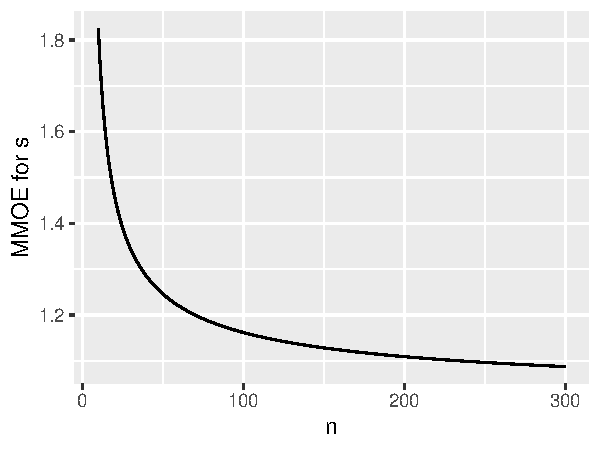
\includegraphics[width=\maxwidth]{htest-smmoe-1} }

\caption[Margin of error in estimating $\sigma$]{Multiplicative margin of error in estimating $\sigma$ as a function of sample size, with 0.95 confidence}\label{fig:htest-smmoe}
\end{figure}
\end{Schunk}
From the above calculations, to achieve a MMOE of no worse than 1.2
with 0.95 confidence when estimating $\sigma$ requires a sample size
of 70 subjects.  A pilot study with $n=20$ will achieve a
MMOE of 1.46 in estimating $\sigma$.

\subsection{Problems with Standardized Effect Sizes}
Many researchers use Cohen's standardized effect sizes in planning a
study. This has the advantage of not requiring pilot data. But such
effect sizes are not biologically meaningful and may hide important
issues~\cite{len01som}. Studies should be designed on the basis
of effects that are relevant to the investigator and human
subjects. If, for example, one plans a study to detect a one standard
deviation (SD) difference in the means and the SD is large, one can
easily miss a biologically important difference that happened to be
much less than one SD in magnitude. Note that the SD is a measure of
how subjects disagree with one another, not a measure of an effect
(e.g., the shift in the mean).  One way to see that standardized
effect sizes are problematic is to note that if one were to make the
measurements more noisy, the SD will increase and the purported
clinically important difference to detect will increase proportionately.

\subsection{Choice of Effect Size}
If a study is designed to detect a certain effect size with a given
power, the effect size should never be the observed effect from
another study, which may be estimated with error and be overly
optimistic. The effect size to use in planning should be the
clinically or biologically relevant effect one would regret
missing.  Usually the only information from prior studies that is
useful in sample size estimation are (in the case of a continuous
response variable with a symmetric distribution) estimates of the
standard deviation or the correlation between two measurements on the
same subject measured at two different times, or (in the case of a
binary or time to event outcome) event probabilities in control
subjects.  An excellent resource by Senn for understanding effect
sizes in power calculations may be found \href{https://errorstatistics.com/2014/03/17/stephen-senn-on-how-to-interpret-discrepancies-against-which-a-test-has-high-power-guest-post/amp}{here}.

\subsection{Multiple Estimands and Hypotheses}
In many experiments there are more than one estimand (what is to be
estimated based on the question of interest) or hypothesis.  Some
frequentist statisticians and biomedical investigators believe that in such
situations the familywise error probability should be
controlled\footnote{As stated elsewhere, multiplicity adjustments are
  a byproduct of faults in frequentist inference and are completely arbitrary.}.
This probability is the probability of rejecting \emph{any} null
hypothesis given that \emph{all} null hypotheses are true.  One may
accomplish this by testing every hypothesis at the $\alpha^{*}$ level,
where the constant $\alpha^{*} < \alpha$ is chosen so that the overall
type one error is $\alpha$, or one may elect to
differentially ``spend $\alpha$'' by, for example, setting $\alpha=0.04$ for a
primary hypothesis and $\alpha=0.01$ for a less important secondary
analysis.  Another alternative is closed testing procedures whereby
later hypotheses can be tested at less stringent $\alpha$ levels as
long as all earlier hypotheses were rejected.  Unfortunately there is
no unique path to deriving multiplicity adjustments, and they have the
odd property of requiring one to be more stringent in assessing
evidence for one hypothesis just because one had other hypotheses.

An alternative, and what we believe to be more reasonable, view is by
Cook and Farewell~\cite{coo96mul} who stated that if a study has more
than one question and each question is to be answered on its own,
there is no need for a multiplicity adjustment.  This is especially
true if a strong priority ordering for hypotheses is stated in
advance.  For example, an investigator may specify three hypotheses about
efficacy of a treatment for the following
endpoints in a cardiovascular trial, sorted from most important to
least important: overall mortality, cardiovascular mortality,
and cardiovascular death or myocardial infarction.  As long as the
researcher always reports all of the results in context, in this
pre-specified order, each $P$-value can stand on its own.

Contrast this with an exploratory study in which the hypothesis is
essentially that there exists an endpoint for which the treatment is
effective.  One should expect to have to employ a conservative
multiplicity adjustment in that situation, e.g., Bonferroni's inequality.

\section{Comprehensive Example: Two sample $t$-test}

\subsection{Study Description}

\bi
\item Compare the effects of two soporific drugs
 \bi
 \item Optical isomers of hyoscyamine hydrobromide
 \ei
\item Parallel-group randomized controlled trial
\item Each subject receives a placebo and then is randomly assigned to receive Drug 1 or Drug 2
\item Dependent variable: Number of hours of increased sleep over
  placebo run-in period.  This should be checked to be a proper change score.

\item Drug 1 given to $n_1$ subjects, Drug 2 given to $n_2$ different subjects
\item Study question: Is Drug 1 or Drug 2 more effective at increasing sleep?
  \bi
  \item $H_0: \mu_1 = \mu_2$
  \item $H_1: \mu_1 \neq \mu_2$
  \ei
\ei

\subsection{Power and Sample Size}

\bi
\item Pilot study or previous published research shows $\sigma = 1.9$ hours
\item Determine the number of subjects needed (in each group) for several value of effect size $\Delta$ ($\Delta = |\mu_1 - \mu_2|$) in order to have 0.9 power with $\alpha = 0.05$
\ei

\begin{table}[!hbp]
 \begin{center}
 \begin{tabular}{lrrrrr} \hline\hline
$\Delta$ &$ 1.0$&$ 1.5$&$ 2.0$&$2.5$ & $3.0$ \\ 
$n$ &$77$&$35$&$20$&$14$&$10$ \\\hline \hline
\end{tabular}
\end{center}

\end{table}

\bi
\item If Drug 1 (or 2) increases sleep by 3.0 hours more than Drug 2 (or 1), by enrolling 10 subjects in each group we will have 0.9 power to detect an association
\ei

\subsection{Collected Data}
\begin{table}[!hbp]
 \begin{center}
 \begin{tabular}{lrr}\hline\hline
Obs. & \multicolumn{1}{c}{Drug 1}&
\multicolumn{1}{c}{Drug 2}
\\ \hline
1 & $ 0.7$&$ 1.9$\\
2 & $-1.6$&$ 0.8$\\
3 & $-0.2$&$ 1.1$\\
4 & $-1.2$&$ 0.1$\\
5 & $-0.1$&$-0.1$\\
6 & $ 3.4$&$ 4.4$\\
7 & $ 3.7$&$ 5.5$\\
8 & $ 0.8$&$ 1.6$\\
9 & $ 0.0$&$ 4.6$\\
10 & $ 2.0$&$ 3.4$\\
& & \\
Mean & $ 0.75$&$ 2.33$\\
SD & $ 1.79$&$ 2.0$\\
\hline
\end{tabular}
\end{center}
\end{table}

\begin{Schunk}
\begin{Sinput}
require(ggplot2)   # Fig (*\ref{fig:htest-sleepa}*)
sleep <- data.frame(drug=c(rep('Drug 1', 10), rep('Drug 2', 10)),
                    extra=c(.7, -1.6, -.2, -1.2, -.1, 3.4, 3.7, .8, 0, 2,
                      1.9, .8, 1.1, .1, -.1, 4.4, 5.5, 1.6, 4.6, 3.4))
ggplot(sleep, aes(x=drug, y=extra, group=drug)) +
  geom_boxplot(col='lightyellow1', alpha=.3, width=.3) + 
  geom_dotplot(binaxis='y', stackdir='center', position='dodge') +
  stat_summary(fun.y=mean, geom="point", col='red', shape=5, size=3) +
  xlab('') + ylab('Extra Hours of Sleep') + coord_flip() 
\end{Sinput}
\begin{figure}[htbp]

\centerline{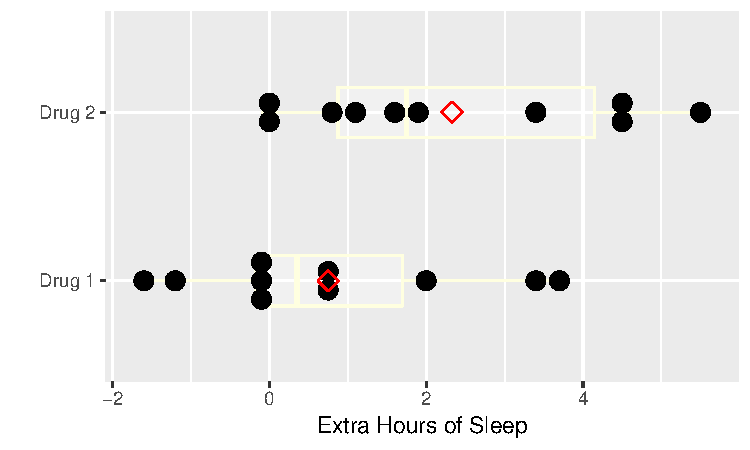
\includegraphics[width=\maxwidth]{htest-sleepa-1} }

\caption[Two-sample parallel group RCT]{Data for two-sample RCT.  Measurements are differences from a control period while subjects were on placebo.  Control period data were not used in the analysis except for normalization.  Diamonds depict means.}\label{fig:htest-sleepa}
\end{figure}
\end{Schunk}

\subsection{Statistical Test}
It is more accepted in practice to now use the form of the $t$-test
that does not assume equal variances in the two independent groups.
The unequal-variance $t$-test is used here.
\begin{Schunk}
\begin{Sinput}
t.test(extra ~ drug, data=sleep)
\end{Sinput}
\begin{Soutput}

	Welch Two Sample t-test

data:  extra by drug
t = -1.8608, df = 17.776, p-value = 0.07939
alternative hypothesis: true difference in means is not equal to 0
95 percent confidence interval:
 -3.3654832  0.2054832
sample estimates:
mean in group Drug 1 mean in group Drug 2 
                0.75                 2.33 
\end{Soutput}
\end{Schunk}
\bi
\item Interpretation
 \bi
 \item Compare Drug 2 to Drug 1.  The output compares 1 to 2
 \item Individuals who take Drug 2 sleep on average 1.58 hours longer (0.95 CI: [-0.21, 3.37]) than individuals who take Drug 1
 \ei
\ei

\clearpage
\section{Comprehensive Example: Paired $t$-test}

\subsection{Study Description}

\bi
\item Compare the effects of two soporific drugs.
\item Crossover study (hopefully with randomized order)
\item Each subject receives placebo run-in, then Drug 1, then Drug 2
\item Investigator did not know about randomized crossover studies
\item Dependent variable: Number of hours of increased sleep when
  compared to a placebo run-in period (raw data not shown)
\item Drug 1 given to $n$ subjects, Drug 2 given to same $n$ subjects
\item Study question: Is Drug 1 or Drug 2 more effective at increasing sleep?
  \bi
  \item $H_0: \mu_d = 0 \hspace{.2cm} \textrm{where} \hspace{.2cm} \mu_d = \mu_1 - \mu_2$
  \item $H_1: \mu_d \neq 0$
  \ei
\ei


\subsection{Power and Sample Size}

\bi
\item Pilot study or previous published research shows the standard deviation of the difference ($\sigma_d$) is $1.2$ hours
\item Determine the number of subjects needed for several value of effect size $\Delta$ ($\Delta = |\mu_1 - \mu_2|$)with 0.9 power, $\alpha = 0.05$
\ei

\begin{table}[!hbp]
 \begin{center}
 \begin{tabular}{lrrrr}\hline\hline
$\Delta$ &$ 0.5$&$ 1$&$1.5$&$2$\\
$n$ &$62$&$16$&$8$&$5$\\
\hline
\end{tabular}
\end{center}
\end{table}

\bi
\item If Drug 1 (or 2) increases sleep by 1.5 hours more than Drug 2 (or 1), by enrolling 8 subjects we will have 0.9 power to detect an association.
\item More powerful than the two sample test (need 10 subjects in each group for $\Delta = 3.0$ hours)
\ei
\subsection{Collected Data}
Here are the data for the 10 subjects.
\begin{table}[!hbp]
 \begin{center}
 \begin{tabular}{lrrr}\hline\hline
Subject & Drug 1 & Drug 2 & {\color{red}Diff (2-1)}
\\ \hline
1 & $ 0.7$&$ 1.9$&$\color{red}1.2$\\
2 &$-1.6$&$ 0.8$&$\color{red}2.4$\\
3 &$-0.2$&$ 1.1$&$\color{red}1.3$\\
4 &$-1.2$&$ 0.1$&$\color{red}1.3$\\
5 &$-0.1$&$-0.1$&$\color{red}0.0$\\
6 &$ 3.4$&$ 4.4$&$\color{red}1.0$\\
7 &$ 3.7$&$ 5.5$&$\color{red}1.8$\\
8 &$ 0.8$&$ 1.6$&$\color{red}0.8$\\
9 &$ 0.0$&$ 4.6$&$\color{red}4.6$\\
10 &$ 2.0$&$ 3.4$&$\color{red}1.4$\\ \\
Mean & $ 0.75$&$ 2.33$&$\color{red}1.58$\\
SD & $ 1.79$&$ 2.0$&$\color{red}1.2$\\
\hline
\end{tabular}\alabel{sleeppaired}
\end{center}
\end{table}
\begin{Schunk}
\begin{Sinput}
drug1 <- c(.7, -1.6, -.2, -1.2, -.1, 3.4, 3.7, .8, 0, 2)
drug2 <- c(1.9, .8, 1.1, .1, -.1, 4.4, 5.5, 1.6, 4.6, 3.4)
d <- data.frame(Drug=c(rep('Drug 1', 10), rep('Drug 2', 10),
                  rep('Difference', 10)),
                extra=c(drug1, drug2, drug2 - drug1))
w <- data.frame(drug1, drug2, diff=drug2 - drug1)

ggplot(d, aes(x=Drug, y=extra)) +   # Fig. (*\ref{fig:htest-tplot}*)
  geom_boxplot(col='lightyellow1', alpha=.3, width=.5) + 
  geom_dotplot(binaxis='y', stackdir='center', position='dodge') +
  stat_summary(fun.y=mean, geom="point", col='red', shape=18, size=5) +
  geom_segment(data=w, aes(x='Drug 1', xend='Drug 2', y=drug1, yend=drug2),
               col=gray(.8)) +
  geom_segment(data=w, aes(x='Drug 1', xend='Difference', y=drug1, yend=drug2 - drug1),
               col=gray(.8)) +
  xlab('') + ylab('Extra Hours of Sleep') + coord_flip() 
\end{Sinput}
\begin{figure}[htbp]

\centerline{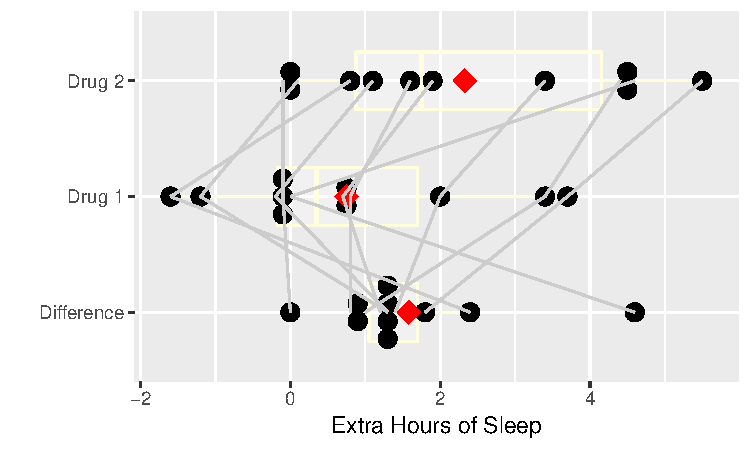
\includegraphics[width=\maxwidth]{htest-tplot-1} }

\caption[Data and box plots for paired data]{Raw data and box plots for paired data and their paired differences, with lines connecting points from the same subject.  Diamonds depict means.}\label{fig:htest-tplot}
\end{figure}
\end{Schunk}

\subsection{Statistical Test}
\begin{Schunk}
\begin{Sinput}
with(d, t.test(drug1, drug2, paired=TRUE))
\end{Sinput}
\begin{Soutput}

	Paired t-test

data:  drug1 and drug2
t = -4.0621, df = 9, p-value = 0.002833
alternative hypothesis: true difference in means is not equal to 0
95 percent confidence interval:
 -2.4598858 -0.7001142
sample estimates:
mean of the differences 
                  -1.58 
\end{Soutput}
\end{Schunk}
\bi
\item Interpretation
 \bi
 \item A person who takes Drug 2 sleeps on average 1.58 hours longer (0.95 CI: [0.70, 2.46]) than a person who takes Drug 1
 \ei
\item Note: Same point estimate (1.58 hours), but more precise estimate (tighter CI) than the 2-sample $t$-test
\ei

\clearpage
\section{Comprehensive Example: Crossover design and analysis}
\bi
 \item In the previous example, it was not clear if the order of placebo, Drug 1, and Drug 2 was the same for every patient
 \item In a cross-over design, each patient receives both drugs
   \bi
     \item Can serve as own control
     \item Order is randomized
   \ei
 \item Carryover effects
   \bi
      \item Def: An effects that carries over from one experimental condition to another
      \item Need a washout period between drugs to remove carryover effects
      \item Time to remove carryover effects should be based on science, not statistics
      \item Statistical tests for carryover effects are often not
        precise enough to make definitive conclusions (see example) 
      \item The test for carryover is correlated with the overall
        test of efficacy
      \item Pre-testing for carryover then deciding whether to only
        use phase 1 data results in a huge inflation of type I error
        in the test for efficacy
   \ei
\ei

\subsection{Study Description}

\bi
\item Compare the effects of two soporific drugs.
\item Each subject either (1) starts with Drug 1 and crosses over to Drug 2 or (2) starts with Drug 2 and crosses over to Drug 1
  \bi
    \item No placebo run-in in this example
    \item Order randomly assigned
    \item Suitable period of time ($\sim 5$ half-lives) between drug
      crossovers to washout effects of previous drug 
  \ei
\item Dependent variable: Number of hours of sleep on each drug
\item Drug 1 given to $n$ subjects, Drug 2 given to same $n$ subjects
\item Study question: Is Drug 1 or Drug 2 more effective at increasing sleep?
  \bi
  \item $H_0: \mu_d = 0 \hspace{.2cm} \textrm{where} \hspace{.2cm} \mu_d = \mu_1 - \mu_2$
  \item $H_1: \mu_d \neq 0$
  \ei
\ei


\subsection{Power and Sample Size}

\bi
\item Pilot study or previous published research shows the standard deviation of the difference ($\sigma_d$) is $1.2$ hours
\item Determine the number of subjects needed for several value of effect size $\Delta$ ($\Delta = |\mu_1 - \mu_2|$)with 0.9 power, $\alpha = 0.05$
\item Assume no carryover effects
\ei

\begin{table}[!hbp]
 \begin{center}
 \begin{tabular}{lrrrr}\hline\hline
$\Delta$ &$ 0.5$&$ 1$&$1.5$&$2$\\
$n$ &$62$&$16$&$8$&$5$\\
\hline
\end{tabular}
\end{center}
\end{table}

\bi
\item If Drug 1 (or 2) increases sleep by 1.5 hours more than Drug 2 (or 1), by enrolling 8 subjects we will have 0.9 power to detect an association.
\item Same power calculation as paired $t$-test
\ei

\subsection{Collected Data}
\begin{table}[!htbp]
 \begin{center}
 \begin{tabular}{lrrr}\hline\hline
Subject & Drug 1 & Drug 2 & {\color{red}Diff (2-1)}
\\ \hline
1  &$8.7$ &$ 9.9$&$\color{red}1.2$\\
2  &$6.4$ &$ 8.8$&$\color{red}2.4$\\
3  &$7.8$ &$ 9.1$&$\color{red}1.3$\\
4  &$6.8$ &$ 8.1$&$\color{red}1.3$\\
5  &$7.9$ &$ 7.9$&$\color{red}0.0$\\
6  &$11.4$&$ 12.4$&$\color{red}1.0$\\
7  &$11.7$&$ 13.5$&$\color{red}1.8$\\
8  &$8.8$ &$ 9.6$&$\color{red}0.8$\\
9  &$8.0$ &$ 12.6$&$\color{red}4.6$\\
10 &$10.0$&$ 11.4$&$\color{red}1.4$\\ \\
Mean&$8.75$&$ 10.33$&$\color{red}1.58$\\
SD  &$1.79$&$ 2.0$  &$\color{red}1.2$\\
\hline
\end{tabular}
\end{center}
\end{table}

\subsection{Statistical Tests}
\begin{Schunk}
\begin{Sinput}
drug1 <- c(87, 64, 78, 68, 79, 114, 117, 88, 80, 100)/10
drug2 <- c(99, 88, 91, 81, 79, 124, 135, 96, 126, 114)/10
t.test(drug1, drug2, paired=TRUE)
\end{Sinput}
\begin{Soutput}

	Paired t-test

data:  drug1 and drug2
t = -4.0621, df = 9, p-value = 0.002833
alternative hypothesis: true difference in means is not equal to 0
95 percent confidence interval:
 -2.4598858 -0.7001142
sample estimates:
mean of the differences 
                  -1.58 
\end{Soutput}
\end{Schunk}
\bi
\item Interpretation
 \bi
 \item A person who takes Drug 2 sleeps on average 1.58 hours longer (0.95 CI: [0.70, 2.50]) than a person who takes Drug 1
 \ei
\ei

\subsection{Carryover Effects}

\bi
   \item Is there any evidence for a carryover effect?
   \item Assume that the first 5 subjects received Drug 1 first and the second 5 subjects received drug 2 first
   \item If we assume there are no carryover effects, then the mean difference in sleep for subjects receiving drug 1 first should be \textit{the same} as the mean difference for subjects receiving drug 2 first
   \item Recall that assessing carryover effect distorts the efficacy
     analysis inference
   \item Null hypothesis is that there are no carryover effects
   \item Can rearrange the difference data to clarify the structure
\ei

\begin{table}[!hbp]
 \begin{center}
 \begin{tabular}{lrr}\hline\hline
Subject & Drug 1 First & Drug 2 First
\\ \hline
1 & $\color{red}1.2$ & \\
2 & $\color{red}2.4$ & \\
3 & $\color{red}1.3$ & \\
4 & $\color{red}1.3$ & \\
5 & $\color{red}0.0$ & \\
6 & & $\color{red}1.0$\\
7 & & $\color{red}1.8$\\
8 & & $\color{red}0.8$\\
9 & & $\color{red}4.6$\\
10 & & $\color{red}1.4$\\ \\
Mean & 1.24 & 1.92 \\
SD & 0.85 & 1.55 \\
\hline
\end{tabular}
\end{center}
\end{table}

For this design we might expect the variance of the differences to be
the same for both orders, so we use the equal-variance $t$-test.
\begin{Schunk}
\begin{Sinput}
# Unpaired t-test
t.test((drug2 - drug1)[1:5], (drug2 - drug1)[6:10], var.equal=TRUE)
\end{Sinput}
\begin{Soutput}

	Two Sample t-test

data:  (drug2 - drug1)[1:5] and (drug2 - drug1)[6:10]
t = -0.86152, df = 8, p-value = 0.414
alternative hypothesis: true difference in means is not equal to 0
95 percent confidence interval:
 -2.500137  1.140137
sample estimates:
mean of x mean of y 
     1.24      1.92 
\end{Soutput}
\end{Schunk}
\bi
\item Interpretation
 \bi
 \item Large $P$-value has no interpretation
 \item With 0.95 confidence, the carryover effect is between [-2.5 and 1.1] hours, which is not scientifically convincing either way
 \item In general, be very cautious when the null hypothesis is something you want to fail to reject in order to validate your analysis method
   \bi
     \item Tests of normality are sometimes used to validate using a parametric over a non-parametric test
     \item There are also statistical tests for equal variance
     \item Both tests promote incorrect interpretation of large
       $P$-value as being evidence supporting the null hypothesis 
   \ei
 \ei
\ei



%% Usage: knitr slide

\chapter{Comparing Two Proportions} \ros{10.1-10.3, 10.5}\katz{5.2}\bmovie{8}\ddisc{8}

\section{Overview}

\bi
 \item Compare dichotomous independent variable with a dichotomous outcome
  \bi
  \item Independent variables: Exposed/Not, Treatment/Control, Knockout/Wild Type, etc.
  \item Outcome (dependent) variables: Diseased/Not or any Yes/No outcome 
  \ei
 \item Continuous outcomes often dichotomized for analysis (bad idea)
  \bi
  \item Consider $t$-tests (Chapter 5) or Non-parameteric methods (Chapter 7)
  \ei
\ei

\section{Normal-Approximation Test}
\bi
\item Two independent samples

%, sizes $n_{1}, n_{2}$
%\item Unknown population probabilities of event $p_{1}, p_{2}$
%\item Sample proportions for estimating $p_{1},p_{2}$: $\hat{p}_{1},
%  \hat{p}_{2}$
\begin{tabular}{lcc} 
 & \underline{Sample 1} & \underline{Sample 2} \\
Sample size & $n_1$ & $n_2$ \\
Population probability of event & $p_1$ & $p_2$ \\
Sample probability of event & $\hat{p}_1$ & $\hat{p}_2$ \\
\end{tabular}

\item Null Hypothesis, $H_{0}: p_{1}=p_{2}=p$
\item Estimating the variance
\bi 
 \item Variance of $\hat{p}_{i} = p_{i}(1-p_{i})/n_{i}$ for $i = 1, 2$
 \item Variance of $\left(\hat{p}_1 - \hat{p}_2\right)$ is the sum of the
  variances, which under $H_{0}$ is
   \beq
    p(1-p)[\frac{1}{n_{1}}+\frac{1}{n_{2}}]
   \eeq
 \item We estimate this variance by plugging $\hat{p}$ into $p$, where
 \beq
 \hat{p} = \frac{n_{1}\hat{p}_{1}+n_{2}\hat{p}_{2}}{n_{1}+n_{2}}
 \eeq
 is the pooled estimate of the probability under $H_{0}: p_1 = p_2 = p$
\ei
\item Test statistic which has approximately a normal distribution
  under $H_{0}$ if $n_{i}\hat{p}_{i}$ are each large enough:
\beq
z = \frac{\hat{p}_{1} -
  \hat{p}_{2}}{\sqrt{\hat{p}(1-\hat{p})[\frac{1}{n_{1}}+\frac{1}{n_{2}}]}}
\eeq
\item To test $H_{0}$ we see how likely it is to obtain a $z$ value as
  far or farther out in the tails of the normal distribution than $z$
  is
\item We don't recommend using the continuity correction
\item Example:  \\
Test whether the population of women whose age at first birth $\leq
29$ has the same probability of breast cancer as women whose age at
first birth was $\geq 30$.  This dichotomization is highly arbitrary
and we should really be testing for an association between age and
cancer incidence, treating age as a continuous variable.
\item Case-control study (independent and dependent variables
  interchanged); $p_{1}=$ probability of age at first birth $\geq 30$,
  etc.

\begin{tabular}{lcc} 
 & \underline{with Cancer} & \underline{without Cancer} \\
Total \# of subjects & $3220 (n_1)$ & $10245 (n_2)$ \\
\# age $\geq 30$ & $683$ & $1498$ \\ \\
Sample probabilities & $0.212 (\hat{p}_1$) & $0.146 (\hat{p}_2$) \\ \\
Pooled probability &\multicolumn{2}{c}{$\frac{683 + 1498}{3220 + 10245} = 0.162$} \\
\end{tabular}


%\beqa
%n_{1}=3220, n_{2}=10245, \\ 
%\hat{p}_{1}=\frac{683}{3220}=0.212, \\
%\hat{p}_{2}=\frac{1498}{10245} = 0.146 \\
%\hat{p}=\frac{683+1498}{3220+10245} = 0.162 \\
\item Estimate the variance
  \bi
  \item $\mathrm{variance}(\hat{p}_{1}-\hat{p}_{2}) = \hat{p}(1-\hat{p})\times \left[\frac{1}{n_{1}}+\frac{1}{n_{2}}\right] = 5.54 \times 10^{-5}$ \\
  \item $SE = \sqrt{\mathrm{variance}} = 0.00744$ \\
  \ei
\item Test statistic
  \bi 
  \item $z = \frac{0.212-0.146}{0.00744} = 8.85$
  \ei
\item 2-tailed $P$-value is $ < 10^{-4}$
\begin{Schunk}
\begin{Sinput}
n1 <- 3220;     n2 <- 10245
p1 <- 683 / n1; p2 <- 1498 / n2
pp <- (n1 * p1 + n2 * p2) / (n1 + n2)
se <- sqrt(pp * (1 - pp) * (1 / n1 + 1 / n2))
z  <- (p1 - p2) / se
pval <- 2 * (1 - pnorm(abs(z)))
round(c(p1=p1, p2=p2, pooled=pp, se=se, z=z, pval=pval), 4)
\end{Sinput}
\begin{Soutput}
    p1     p2 pooled     se      z   pval 
0.2121 0.1462 0.1620 0.0074 8.8527 0.0000 
\end{Soutput}
\end{Schunk}
\item We do not use a $t$-distribution because there is no $\sigma$ to
  estimate (and hence no ``denominator d.f.'' to subtract)
\ei

\section{$\chi^2$ Test}
\bi
\item If $z$ has a normal distribution, $z^2$ has a $\chi^2$
  distribution with 1 d.f. (are testing a single difference against zero)
\item The data we just tested can be shown as a $2\times 2$
  contingency table

\begin{tabular}{l|c|c|c} 
\multicolumn{1}{l}{} & \multicolumn{1}{c}{Cancer +} & \multicolumn{1}{l}{Cancer -} \\ \cline{2-3}
Age $\leq 29$ & $2537 $ & $8747$ & $11284$ \\ \cline{2-3}
Age $\geq 30$ & $683$ & $1498$ &  $2181$ \\ \cline{2-3}
\multicolumn{1}{l}{} & \multicolumn{1}{c}{$3220$} & \multicolumn{1}{c}{$10245$} & \multicolumn{1}{c}{$13465$}
\end{tabular}


\item In general, the $\chi^2$ test statistic is given by
\beq
\sum_{ij} \frac{(\textrm{Obs}_{ij}-\textrm{Exp}_{ij})^2}{\textrm{Exp}_{ij}}
% \frac{(\textrm{Observed_{ij}} - \textrm{Expected_{ij}})^2}{\textrm{Expected_{ij}}}$
\eeq
\item $\textrm{Obs}_{ij}$ is the observed cell frequency for row $i$ column $j$
\item $\textrm{Exp}_{ij}$ is the expected cell frequency for row $i$ column $j$
  \bi
  \item Expected cell frequencies calculating assuming $H_0$ is true
  \item $\textrm{Exp}_{ij} = \frac{\textrm{row $i$ total} \times \textrm{column $j$ total}}{\textrm{grand total}}$
  \item e.g. $\textrm{Exp}_{11} = \frac{11284 \times 3220}{13465} = 2698.4$
  \ei

\item For $2 \times 2$ tables, if the observed cell frequencies are labeled
\begin{tabular}{|c|c|} \hline
$a$ & $b$ \\ \hline
$c$ & $d$ \\ \hline
\end{tabular}
the $\chi^{2}$ test statistic simplifies to
\beq
\frac{N[ad - bc]^{2}}{(a+c)(b+d)(a+b)(c+d)},
\eeq
where $N=a+b+c+d$.  Here we get $\chi^{2}_{1} = 78.37$
\item 78.37 is $z^2$ from above!
\begin{Schunk}
\begin{Sinput}
x <- matrix(c(2537, 8747, 683, 1498), nrow=2, byrow=TRUE)
x
\end{Sinput}
\begin{Soutput}
     [,1] [,2]
[1,] 2537 8747
[2,]  683 1498
\end{Soutput}
\begin{Sinput}
chisq.test(x, correct=FALSE)
\end{Sinput}
\begin{Soutput}

	Pearson's Chi-squared test

data:  x
X-squared = 78.37, df = 1, p-value < 2.2e-16
\end{Soutput}
\begin{Sinput}
# Also compute more accurate P-value based on 1M Monte-Carlo simulations
chisq.test(x, correct=FALSE, simulate.p.value=TRUE, B=1e6)
\end{Sinput}
\begin{Soutput}

	Pearson's Chi-squared test with simulated p-value (based on 1e+06
	replicates)

data:  x
X-squared = 78.37, df = NA, p-value = 1e-06
\end{Soutput}
\end{Schunk}
\item Don't need Yates' continuity correction
%  Eq.\ 10.5
\item Note that even though we are doing a 2-tailed
test we use only the right tail of the $\chi^{2}_{1}$ distribution;
that's because we have squared the difference when computing the
statistic, so the sign is lost.
\item This is the ordinary Pearson $\chi^2$ test
\ei

\section{Fisher's Exact Test}
\bi
\item Is a misnomer in the sense that it computes probabilities
  exactly, with no normal approximation, but only after changing what
  is being tested to condition on the number of events and non-events
\item Because frequencies are discrete and because of the
  conditioning, the test is conservative ($P$-values too large)
\item Is exact only in the sense that actual type I error probability will not \textbf{exceed} the nominal level
\item The ordinary Pearson $\chi^2$ works fine (even when
  an expected cell frequency is as low as 1.0, contrary to popular belief)
\item We don't use Yates' continuity correction because it was
  developed to make the normal approximation test yield $P$-values
  that are more similar to Fisher's test, i.e., to be more
  conservative
\item The attempt to obtain exact unconditional $P$-values for the simple $2\times 2$ contingency table has stumped frequentist statisticians for many decades~\cite{cho15elu}
\item By contrast, Bayesian posterior probabilities for the true unconditional quantity of interest are exact
 \bi
 \item Frequentist confidence limits and $P$-values are approximate because they use the sample space, and the sample space is discrete when the response variable is categorical
 \item Bayes does not consider the sample space, only the parameter space, which is almost always continuous
 \ei
\item See \href{https://stats.stackexchange.com/questions/14226}{stats.stackexchange.com/questions/14226} for discussion
\ei

\section{Sample Size and Power for Comparing Two Independent Samples}
\bi
\item Power $\uparrow$ as
 \bi
 \item $n_{1}, n_{2} \uparrow$
 \item $\frac{n_{2}}{n_{1}} \rightarrow 1.0$ (usually)
 \item $\Delta = |p_{1}-p_{2}| \uparrow$
 \item $\alpha \uparrow$
 \ei
\item There are approximate formulas such as the recommended methods in Altman based on transforming $\hat{p}$ to make it have a
  variance that is almost independent of $p$ \altman{45-50}
\item Example:  \\

Using current therapy, 0.5 of the population is free of infection at 24 hours.  Adding a new drug to the standard of care is expected to increase the percentage infection-free to 0.7.  If we randomly sample 100 subjects to receive standard care and 100 subjects to receive the new therapy, what is the probabilty that we will be able to detect a certain difference between the two therapies at the end of the study?

\beq
p_{1}=.5, p_{2}=.7, n_{1}=n_{2}=100
\eeq
results in a power of 0.83 when $\alpha=0.05$
\begin{Schunk}
\begin{Sinput}
require(Hmisc)
bpower(.5, .7, n1=100, n2=100)
\end{Sinput}
\begin{Soutput}
    Power 
0.8281098 
\end{Soutput}
\end{Schunk}
\item When computing sample size to achieve a given power, the sample
  size $\downarrow$ when
 \bi
 \item power $\downarrow$
 \item $\frac{n_{2}}{n_{1}} \rightarrow 1.0$
 \item $\Delta \uparrow$
 \item $\alpha \uparrow$
 \ei
\item Required sample size is a function of both $p_{1}$ and $p_{2}$
\item Example:

How many subjects are needed to detect a 0.8 fold decrease in the probability of colorectal cancer if the baseline probability of cancer is $0.0015$?  Use a power of 0.8 and a type-I error probability of 0.05.

\beqa
p_{1}=0.0015, p_{2}=0.8\times p_{1}=0.0012, \alpha=0.05, \beta=0.2 \\
n_{1}=n_{2}=235,147
\eeqa
(Rosner estimated 234,881)
\ei
\begin{Schunk}
\begin{Sinput}
bsamsize(.0015, 0.8 * .0015, alpha=0.05, power=0.8)
\end{Sinput}
\begin{Soutput}
      n1       n2 
235147.3 235147.3 
\end{Soutput}
\end{Schunk}

Formulas for power and sample size may be seen as \R\ code found at\\
\href{https://github.com/harrelfe/Hmisc/blob/master/R/bpower.s}{github.com/harrelfe/Hmisc/blob/master/R/bpower.s}.

\section{Confidence Interval}
An approximate $1-\alpha$ 2-sided CL is given by
\beq
\hat{p}_{1}-\hat{p}_{2} \pm z_{1-\alpha/2} \times\sqrt{\frac{\hat{p}_{1}(1-\hat{p}_{1})}{n_{1}}+\frac{\hat{p}_{2}(1-\hat{p}_{2})}{n_{2}}}
\eeq
where $z_{1-\alpha/2}$ is the critical value from the normal
distribution (1.96 when $\alpha=0.05$).

The CL for the number of patients needed to be treated to save one
event may simply be obtained by taking the reciprocal of the two
confidence limits.\footnote{If a negative risk reduction is included
  in the confidence interval, set the NNT to $\infty$ for that limit
  instead of quoting a negative NNT.  There is more to this; see \href{http://bit.ly/datamethods-nnt}{bit.ly/datamethods-nnt}.}

\section{Sample Size for a Given Precision}

\bi
 \item Goal: Plan a study so that the margin of error is sufficiently small
 \item The margin of error ($\delta$) is defined to be half of the confidence interval width.  For two proportions,
  \beq
  \delta = z_{1-\alpha/2} \times\sqrt{\frac{\hat{p}_{1}(1-\hat{p}_{1})}{n_{1}}+\frac{\hat{p}_{2}(1-\hat{p}_{2})}{n_{2}}}
  \eeq
 \item Basing the sample size calculations on the margin of error can lead to a study that gives \textit{scientifically} relevant results even if the results are not \textit{statistically} significant.
  \item Example: Suppose that the infection risk in a population is $0.5$ and a reduction to $0.4$ is believed to be a large enough reduction that it would lead to a change in procedures.  A study of a new treatment is planned so that enough subjects will be enrolled for the margin of error is $0.05$.  Consider these two possible outcomes:
  \begin{enumerate}
  \item The new treatment is observed to decrease infections by $0.06$ ($0.95$ CI: $[0.11, 0.01]$).  The confidence interval does not contain $0$, so we have indirect evidence\footnote{To obtain direct evidence requires Bayesian posterior probabilities.} that the new treatment is effective at reducing infections.  $0.1$ is also within the confidence interval limits.
  \item The new treatment is observed to decrease infections by only $0.04$ ($0.95$ CI: $[0.09, -0.01]$).  The confidence interval now contains $0$, so we do not have enough evidence to reject the supposition that there is no effect of the treatment on reducing infections if we are bound to an arbitrary $\alpha=0.05$. However, the confidence interval also does not contain $0.10$, so we are able to indirectly rule out a \textit{scientifically} relevant decrease in infections.
  \end{enumerate}


 \item For fixed $n_{1} = n_2 = n$, confidence intervals for proportions have the maximum width, when $p_{1} = p_{2} =  0.5$.  This can be shown by:
  \bi
  \item Recall that the variance formula for the difference in two proportions when calculating a confidence interval is 
   \beq
   \frac{p_{1}(1-p_{1})}{n_{1}}+\frac{p_{2}(1-p_{2})}{n_{2}}
    \eeq
  \item When $p_{1} = p_{2} =  p$ and $n_{1} = n_2 = n$, the variance formula simplifies to 
    \beq
     \frac{p(1 - p)}{n}+\frac{p (1- p)}{n} = 2\frac{p(1 - p)}{n}
    \eeq
   \item Then, for any fixed value of $n$ ($e.g. n = 1$ or $10$), $2\frac{p(1 - p)}{n}$ is largest when $p = 0.5$.  With $p= 0.5$, the variance formula further simplifies to
    \beq
     2\frac{.25}{n} = \frac{1}{2n}
    \eeq
  \ei
 \item Using $\alpha = 0.05$ ($z_{1-\alpha/2} = 1.96$), the worst-case margin of error will be
    \beq
     \delta = 1.96 \sqrt{\frac{1}{2n}}
    \eeq
 \item By solving for $n$, we can rearrange this formula to be
    \beq
     n = \frac{1.92}{\delta^2}
    \eeq
 \item This formula then gives the number of subjects needed in each group $n$ to obtain a given margin of error $\delta$.  For a margin of error of $0.05$ ($\delta = 0.05$), $n = \frac{1.92}{0.05^2} = 768$ subjects in each group.
\begin{Schunk}
\begin{Sinput}
diff <- .05
qnorm(.975)^2 / 2 / (diff ^ 2)
\end{Sinput}
\begin{Soutput}
[1] 768.2918
\end{Soutput}
\end{Schunk}
\ei

%In the case $n_{1}=n_{2}=n, \alpha=0.05$, the confidence interval has maximum width with $p_{1}$ and $p_{2}$ are near 0.5.  As a worse case the margin of error is then $1.96/\sqrt{2n}$.  The $n$ required to achieve a margin of error of $\delta$ at the 0.95 confidence level is $1.92/\delta^{2}$.  For example, to approximate the difference in the incidence probability of stroke between males and females to at worst $\pm 0.05$ at the 0.95 level would require 768 patients in each group.

\section{Relative Effect Measures}\alabel{sec:prop-rem}
\bi
\item We have been dealing with risk differences which are measures of
  absolute effect
\item Measures of relative effect include risk ratios and odds ratios
\item Risk ratios are easier to interpret but only are useful over a
  limited range of prognosis (i.e., a risk factor that doubles your
  risk of lung cancer cannot apply to a subject having a risk above
  0.5 without the risk factor)
\item Odds ratios can apply to any subject
\item In large clinical trials treatment effects on lowering
  probability of an event are often constant on the odds ratio scale
\item OR = Odds ratio =
  $\frac{\frac{p_{1}}{1-p_{1}}}{\frac{p_{2}}{1-p_{2}}}$
\item Testing $H_{0}$: OR=1 is equivalent to testing
  $H_{0}:p_{1}=p_{2}$
\item There are formulas for computing confidence intervals for odds
  ratios
\item Odds ratios are most variable when one or both of the
  probabilities are near 0 or 1
\item We compute CLs for ORs by anti-logging CLs for the log OR
\item In the case where $p_{1}=p_{2}=0.05$ and $n_{1}=n_{2}=n$, the
  standard error of the log odds ratio is approximately
  $\sqrt{\frac{42.1}{n}}$
\item The common sample size $n$ needed to estimate the true OR to
  within a factor of 1.5 is 984 with $p$s in this range
\item To show the multiplicative margins of error\footnote{Value by
    which to multiply the observed odds ratio to obtain the upper 0.95
    confidence limit or to divide the observed odds ratio to obtain
    the lower 0.95 limit.  The confidence interval for a ratio should
    always be constructed on the log scale (unless using the excellent
    profile likelihood interval which is transformation-invariant).
    We compute the margin of error on the log ratio scale just as we
    do for means.  The margin of error can be defined as $\frac{1}{2}$
    of the width of the confidence interval for the log ratio. If you
    antilog that margin of error you get the multiplicative factor,
    i.e., the multiplicative margin of error.  Suppose that the MMOE
    is 1.5. This means that you can get the 0.95 confidence interval
    for the ratio by taking the ratio’s point estimate and dividing it
    by 1.5 and then multiplying it by 1.5. You can loosely say that
    our point estimate can easily be off by a factor of 1.5.} for a
  range of sample sizes and values of $p$.  For each scenario, the
  margin of error assumes that both unknown probability estimates equal $p$.
\ei
\begin{Schunk}
\begin{Sinput}
require(ggplot2)
d <- expand.grid(n=c(seq(10, 1000, by=10), seq(1100, 50000, by=100)),
                 p=c(.02, .05, .075, .1, .15, .2, .25, .3, .4, .5))
d$selor <- with(d, sqrt(2 / (p * (1 - p) * n)))
d$mmoe  <- with(d, exp(qnorm(0.975) * selor))
mb <- c(1, 1.25, 1.5, 2, 2.5, 3, 4, 5, 10, 20, 30, 40, 50, 100, 400)
ggplot(aes(x=n, y=mmoe, color=factor(p)), data=d) +   # Fig. (*\ref{fig:prop-mmeor}*)
  geom_line() +
  scale_x_log10(breaks=c(10,20,30,50,100,200,500,1000,2000,5000,10000,
                  20000,50000)) +
  scale_y_log10(breaks=mb, labels=as.character(mb)) +
  xlab(expression(n)) + ylab('Multiplicative Margin of Error for OR') +
  guides(color=guide_legend(title=expression(p)))
\end{Sinput}
\begin{figure}[htbp]

\centerline{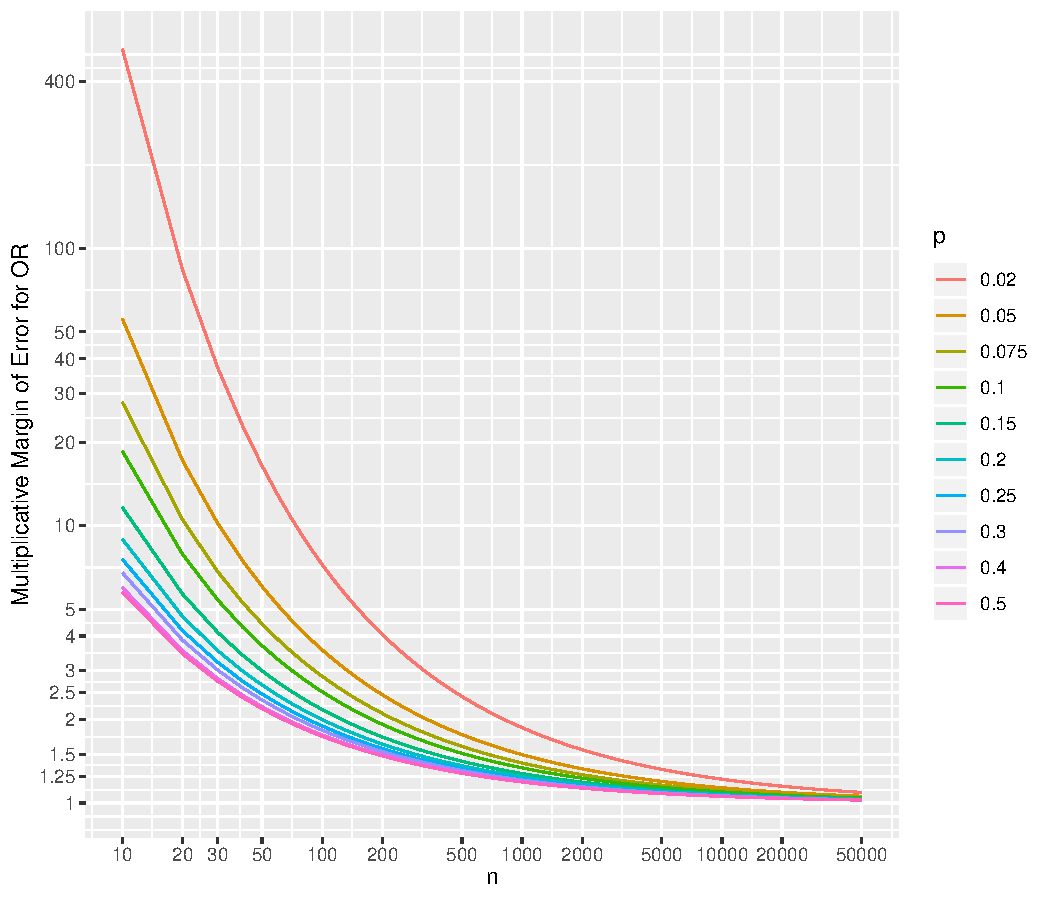
\includegraphics[width=\maxwidth]{prop-mmeor-1} }

\caption[Multiplicative margin of error for odds ratios]{Multiplicative margin of error related to 0.95 confidence limits of an odds ratio, for varying $n$ and $p$ (different curves), assuming the unknown true probability in each group is no lower than $p$}\label{fig:prop-mmeor}
\end{figure}
\end{Schunk}


\section{Comprehensive example}

\subsection{Study Description}
\bi
  \item Consider patients who will undergo coronary artery bypass graft surgery (CABG)
  \item Mortality risk associated with open heart surgery
  \item Study question: Do emergency cases have a surgical mortality that is different from that of non-emergency cases?
  \item Population probabilities
  \bi
    \item $p_1$: Probability of death in patients with emergency priority
    \item $p_2$: Probability of death in patients with non-emergency priority
  \ei
  \item Statistical hypotheses
  \bi
  \item $H_0: p_1 = p_2$ (or $\textrm{OR} = 1$)
  \item $H_1: p_1 \neq p_2$ (or $\textrm{OR} \neq 1$)
  \ei
\ei

\subsection{Power and Sample Size}

\bi
  \item Prior research shows that just over $0.1$ of surgeries end in death
  \item Researchers want to be able to detect a 3 fold increase in risk
  \item For every 1 emergency priority, expect to see 10 non-emergency
  \item $p_1 = 0.3$, $p_2 = 0.1$, $\alpha = 0.05$, and $\textrm{power} = 0.90$
  \item Calculate sample sizes using the PS software for these values and other combinations of $p_1$ and $p_2$
\ei

\begin{table}[!hbp]
 \begin{center}
 \begin{tabular}{lcccc} \hline\hline
$(p_1, p_2)$ &\boldmath$(0.3, 0.1)$&$(0.4, 0.2)$&$(0.03, 0.01)$&$(0.7, 0.9)$ \\ 
$n_1$  &\boldmath$40$&$56$&$589$&$40$ \\ 
$n_2$  &\boldmath$400$&$560$&$5890$&$400$ \\ \hline \hline
\end{tabular}
\end{center}
\end{table}
Check PS calculations against the \R\ \Co{Hmisc} package's
\Co{bsamsize} function.
\begin{Schunk}
\begin{Sinput}
round(bsamsize(.3, .1, fraction=1/11, power=.9))
\end{Sinput}
\begin{Soutput}
 n1  n2 
 40 399 
\end{Soutput}
\begin{Sinput}
round(bsamsize(.4, .2, fraction=1/11, power=.9))
\end{Sinput}
\begin{Soutput}
 n1  n2 
 56 561 
\end{Soutput}
\begin{Sinput}
round(bsamsize(.7, .9, fraction=1/11, power=.9))
\end{Sinput}
\begin{Soutput}
 n1  n2 
 40 399 
\end{Soutput}
\end{Schunk}

\subsection{Collected Data}

In-hospital mortality figures for emergency surgery and other surgery

\begin{table}[!hbp]
 \begin{center}
 \begin{tabular}{l|cc}
 & \multicolumn{2}{|c}{Discharge Status} \\
Surgical Priority& Dead& Alive \\ \hline
Emergency&$6$&$ 19$\\
Other&$11$&$100$\\
\end{tabular}
\end{center}
\end{table}

\bi
\item $\hat{p}_1 = \frac{6}{25} = 0.24$
\item $\hat{p}_2 = \frac{11}{111} = 0.10$
\ei

\subsection{Statistical Test}
\begin{Schunk}
\begin{Sinput}
n1 <- 25;     n2 <- 111
p1 <- 6 / n1; p2 <- 11 / n2
or <- p1 / (1 - p1) / (p2 / (1 - p2))
or
\end{Sinput}
\begin{Soutput}
[1] 2.870813
\end{Soutput}
\begin{Sinput}
# Standard error of log odds ratio:
selor <- sqrt(1 / (n1 * p1 * (1 - p1)) + 1 / (n2 * p2 * (1 - p2)))
# Get 0.95 confidence limits
cls <- exp(log(or) + c(-1, 1) * qnorm(0.975) * selor)
cls
\end{Sinput}
\begin{Soutput}
[1] 0.946971 8.703085
\end{Soutput}
\begin{Sinput}
tcls <- paste0(round(or, 2), ' (0.95 CI: [', round(cls[1], 2),
               ', ', round(cls[2], 2), '])')
# Multiplying a constant by the vector -1, 1 does +/-
x <- matrix(c(6, 19, 11, 100), nrow=2, byrow=TRUE)
x
\end{Sinput}
\begin{Soutput}
     [,1] [,2]
[1,]    6   19
[2,]   11  100
\end{Soutput}
\begin{Sinput}
chisq.test(x, correct=FALSE)
\end{Sinput}
\begin{Soutput}

	Pearson's Chi-squared test

data:  x
X-squared = 3.7037, df = 1, p-value = 0.05429
\end{Soutput}
\end{Schunk}
% Ignore the warning about the $\chi^2$ approximation.
\bi
\item Interpretation
 \bi
 \item Compare odds of death in the emergency group
   $\left(\frac{\hat{p}_1}{1-\hat{p}_1}\right)$ to odds of death in
   non-emergency group  $\left(\frac{\hat{p}_2}{1-\hat{p}_2}\right)$ 
 \item Emergency cases have 2.87 (0.95 CI: [0.95, 8.7]) fold
   increased odds of death during surgery compared to
   non-emergency cases. 
 \ei
\ei

\subsubsection{Fisher's Exact Test}

Observed marginal totals from emergency surgery dataset \\
\begin{tabular}{l|c|c|c} 
\multicolumn{1}{l}{} & \multicolumn{1}{c}{Dead} & \multicolumn{1}{l}{Alive} \\ \cline{2-3}
Emergency & $a$ & $b$ & $25$ \\ \cline{2-3}
Other & $c$ & $d$ &  $111$ \\ \cline{2-3}
\multicolumn{1}{l}{} & \multicolumn{1}{c}{$17$} & \multicolumn{1}{c}{$119$} & \multicolumn{1}{c}{$136$}
\end{tabular}

\bi
\item With fixed marginal totals, there are 18 possible tables ($a = 0, 1, \ldots 17$)
\item Can calculated probability of each of these tables
\bi
\item $p$-value: Probability of observing data as extreme or more extreme than we collected in this experiment
\ei
\item Exact test: $p$-value can be calculated ``exactly'' (not using the $\chi^2$ distribution to approximate the $p$-value)
\\
\begin{Schunk}
\begin{Sinput}
fisher.test(x)
\end{Sinput}
\begin{Soutput}

	Fisher's Exact Test for Count Data

data:  x
p-value = 0.08706
alternative hypothesis: true odds ratio is not equal to 1
95 percent confidence interval:
 0.7674155 9.6831351
sample estimates:
odds ratio 
  2.843047 
\end{Soutput}
\end{Schunk}
Note that the odds ratio from Fisher's test is a conditional maximum
likelihood estimate, which differs from the unconditional maximum
likelihood estimate we obtained earlier.
\item Fisher's test more conservative than Pearson's $\chi^2$ test
  (larger $P$-value) 
\ei

\section{Logistic Regression for Comparing Proportions}\bmovie{9}\ddisc{9}
\bi
\item When comparing $\geq 2$ groups on the probability that a categorical outcome variable will have a certain value observed (e.g., $P(Y=1)$), one can use the Pearson $\chi^2$ test for a contengency table (or the less powerful Fisher's ``exact'' test)
\item Such analyses can also be done with a variety of regression models
\item It is necessary to use a regression model when one desires to analyze more than the grouping variable, e.g.
  \bi
  \item analyze effects of two grouping variables
  \item adjust for covariates
  \ei
\item For full generality, the regression model needs to have no restrictions on the regression coefficients
  \bi
  \item Probabilities are restricted to be in the interval $[0,1]$ so an additive risk model cannot fit over a broad risk range
  \item Odds ($\frac{p}{1-p}$) are restricted to be in $[0, \infty]$
  \item Log odds have no restrictions since they can be in $[-\infty, \infty]$
  \ei
\item So log odds is a good basis for regression analysis of categorical $Y$
 \bi
 \item default assumption of additivity of effects needs no restrictions
 \item will still translate to probabilities in $[0,1]$
 \ei
\item The binary logistic regression model is a model to estimate the probability of an event as a flexible function of covariates
\item Let the outcome variable $Y$ have the values $Y=0$ (non-event) or $Y=1$ (event)
\begin{equation}
  \textrm{Prob}(Y = 1 | X) = \frac{1}{1 + \exp(-(\beta_0 + \beta_1 x_1 + \beta_2 x_2 + \beta_3 x_3 + \ldots))}
\end{equation}
\item The sum inside the inner () is called the linear predictor (LP)
\item The binary logistic model relates LP (with no restrictions) to the event probability as so:
\begin{Schunk}
\begin{Sinput}
lp <- seq(-5, 5, length=150)
plot(lp, plogis(lp), xlab='Linear Predictor', ylab='P(Y=1)', type='l')
\end{Sinput}


\centerline{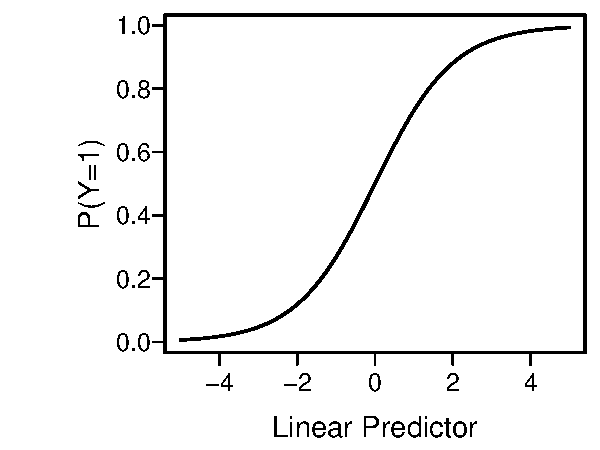
\includegraphics[width=\maxwidth]{prop-lrmshape-1} }

\end{Schunk}
\item Notes about LP:
 \bi 
 \item for a given problem the range may be much narrower than $[-4,4]$
 \item when any predictor $X_j$ with a non-zero $\beta_j$ is categorical, LP cannot take on all possible values within its range, so the above plot will have gaps
 \ei
\item As a special case the model can estimate and compare two probabilities as done above, through an odds ratio
\item Logistic regression seems like an overkill here, but it sets the stage for more complex frequentist analysis as well as Bayesian analysis
\item For our case the model is as follows
\item Consider groups A and B, A = reference group\\
  $[x]$ denotes 1 if $x$ is true, 0 if $x$ is false\\
  Define the expit function as the inverse of the logit function, or expit$(x) = \frac{1}{1 + \exp(-x)}$
\beqa
P(Y = 1 | \textrm{group}) &=& \frac{1}{1 + \exp(-(\beta_0 + \beta_1 [\textrm{group } B]))} \\
 &=& \textrm{expit}(\beta_0 + \beta_1 [\textrm{group } B])\\
P(Y = 1 | \textrm{group A}) &=& \textrm{expit}(\beta_0)\\
P(Y = 1 | \textrm{group B}) &=& \textrm{expit}(\beta_0 + \beta_1)
\eeqa
$\beta_0 =$ log odds of probability of event in group A $= \log(\frac{p_1}{1 - p_1}) = \textrm{logit}(p_1)$\\
$\beta_1 =$ increase in log odds in going from group A to group B = \\ $\log(\frac{p_2}{1 - p_2}) - \log(\frac{p_1}{1 - p_1}) = \textrm{logit}(p_2) - \textrm{logit}(p_1)$\\
$\exp(\beta_1) =$ group B : group A odds ratio $= \frac{\frac{p_2}{1 - p_2}}{\frac{p_1}{1 - p_1}}$ \\
expit$(\beta_0) = p_1$ \\
expit$(\beta_0 + \beta_1) = p_2$
\item Once the $\beta$s are estimated, one quickly gets the B:A odds ratio and $\hat{p}_1$ and $\hat{p}_2$
\item This model is \textbf{saturated}
 \bi
 \item has the maximum number of parameters needed to fully describe the situation (here, 2 since 2 groups)
 \item saturated models \textbf{must} fit the data if the distributional and independence assumptions are met 
 \item logistic model has no distributional assumption
 \ei 
\item Logistic regression is more general and flexible than the specialized tests for proportions
 \bi
 \item allows testing association on continuous characteristics
 \item easily extends to more than two groups
 \item allows adjustment for covariates
 \ei
\item Examples:\\
  \bi
  \item assess effects of subjects' sex and country (Canada vs.\ US) on $P(Y=1)$ denoted by $p$\\
  logit $p$ = constant + logit male effect + logit Canada effect
  \item same but allow for interaction\\
  logit $p$ = constant + logit male effect + logit Canada effect + special effect of being male if Canadian
  \item latter model is saturated with 3 d.f.\ so fits as well as a model with 4 proportions
    \bi
    \item unlike the overall Pearson $\chi^2$ test, allows testing interaction and
    \item separate effects of sex and country (e.g., 2 d.f.\ chunk test for whether there is a sex difference for either country, allowing for the sex effect to differ by country)
    \ei
  \ei
\ei

\subsection{Test Statistics}
For frequentist logistic models there are 3 types of $\chi^2$ test statistics for testing the same hypothesis:
  \bi
  \item likelihood ratio (LR) test (usually the most accurate) and is scale invariant\footnote{The LR test statistic is the same whether testing for an absolute risk difference of 0.0, or for an odds or risk ratio of 1.0.}
   \bi
   \item Can obtain the likelihood ratio $\chi^2$ statistic from either the logistic model or from a logarithmic equation in the two proportions and sample sizes
   \ei
  \item Score test (identical to Pearson test for overall model if model is saturated)
  \item Wald test (square of $\frac{\hat{\beta}}{\textrm{s.e.}}$ in the one parameter case; misbehaves for extremely large effects)
  \item Wald test is the easiest to compute but $P$-values and confidence intervals from it are not as accurate.  The score test is the way to exactly reproduce the Pearson $\chi^2$ statistic from the logistic model.
  \item As with $t$-test vs.\ a linear model, the special case tests are not needed once you use the logistic model framework
  \item Three usages of any of these test statistics:
    \bi
    \item individual test, e.g. sex effect in sex-country model without interaction
    \item chunk test, e.g. sex + sex $\times$ country interaction 2 d.f.\ test\\tests overall sex effect
    \item global test of no association, e.g. 3 d.f.\ test for whether sex or country is associated with $Y$
    \ei
  \ei
 
\subsection{Frequentist Analysis Example}
 \bi
 \item Consider again our emergency surgery example
 \item String the observations out to get one row = one patient, binary $Y$
 \ei

\begin{Schunk}
\begin{Sinput}
require(rms)
\end{Sinput}
\begin{Sinput}
options(prType='latex')
priority <- factor(c(rep('emergency', 25), rep('other', 111)), c('other', 'emergency'))
death <- c(rep(0, 19), rep(1, 6), rep(0, 100), rep(1, 11))
table(priority, death)
\end{Sinput}
\begin{Soutput}
           death
priority      0   1
  other     100  11
  emergency  19   6
\end{Soutput}
\end{Schunk}
\begin{Sinput}
d  <- data.frame(priority, death)
dd <- datadist(d); options(datadist='dd')
# rms package needs covariate summaries computed by datadist
f <- lrm(death ~ priority)
f
\end{Sinput}

 \noindent \textbf{Logistic Regression Model}
 
 \begin{verbatim}
 lrm(formula = death ~ priority)
 \end{verbatim}
 
 {\fontfamily{phv}\selectfont \begin{center}\begin{tabular}{|c|c|c|c|}\hline
&Model Likelihood&Discrimination&Rank Discrim.\\
&Ratio Test&Indexes&Indexes\\\hline
Obs~\hfill 136&LR $\chi^{2}$~\hfill 3.20&$R^{2}$~\hfill 0.044&$C$~\hfill 0.597\\
~~0~\hfill 119&d.f.~\hfill 1&$g$~\hfill 0.319&$D_{xy}$~\hfill 0.193\\
~~1~\hfill 17&Pr$(>\chi^{2})$~\hfill 0.0737&$g_{r}$~\hfill 1.375&$\gamma$~\hfill 0.483\\
$\max|\frac{\partial\log L}{\partial \beta}|$~\hfill $4\!\times\!10^{-9}$&&$g_{p}$~\hfill 0.043&$\tau_{a}$~\hfill 0.043\\
&&Brier~\hfill 0.106&\\
\hline
\end{tabular}
\end{center}}
 
 %latex.default(U, file = "", first.hline.double = FALSE, table = FALSE,     longtable = TRUE, lines.page = lines.page, col.just = rep("r",         ncol(U)), rowlabel = "", already.math.col.names = TRUE,     append = TRUE)%
 \setlongtables\begin{longtable}{lrrrr}\hline
 \multicolumn{1}{l}{}&\multicolumn{1}{c}{$\hat{\beta}$}&\multicolumn{1}{c}{S.E.}&\multicolumn{1}{c}{Wald $Z$}&\multicolumn{1}{c}{Pr$(>|Z|)$}\tabularnewline
 \hline
 \endhead
 \hline
 \endfoot
 Intercept&~-2.2073~&~0.3177~&-6.95&\textless 0.0001\tabularnewline
 priority=emergency&~ 1.0546~&~0.5659~& 1.86&0.0624\tabularnewline
 \hline
 \end{longtable}
 \addtocounter{table}{-1}

\bi 
\item Compare the LR $\chi^2$ of 3.2 with the earlier Pearson $\chi^2$ of 3.70
\item The likelihood ratio (LR) $\chi^2$ test statistic and its $P$-value are usually a little more accurate than the other association tests
 \bi
 \item but $\chi^2$ distribution is still only an approximation to the true sampling distribution
 \ei
\item See that we can recover the simple proportions from the fitted logistic model:\\
$\hat{p}_1 = \frac{11}{111} = 0.099 = \textrm{expit}(-2.2073)$\\
$\hat{p}_2 = \frac{6}{25} = 0.24 = \textrm{expit}(-2.2073 + 1.0546)$
\ei 

\begin{Sinput}
summary(f)
\end{Sinput}
%latex.default(cstats, caption = if (table.env) caption else NULL,     title = title, rowlabel = "", col.just = rep("r", 7), table.env = table.env,     ...)%
\begin{center}
\begin{tabular}{lrrrrrrr}
\hline\hline
\multicolumn{1}{l}{}&\multicolumn{1}{c}{Low}&\multicolumn{1}{c}{High}&\multicolumn{1}{c}{$\Delta$}&\multicolumn{1}{c}{Effect}&\multicolumn{1}{c}{S.E.}&\multicolumn{1}{c}{Lower 0.95}&\multicolumn{1}{c}{Upper 0.95}\tabularnewline
\hline
priority --- emergency:other&1&2&&1.0546&0.56587&-0.054487&2.1637\tabularnewline
~~{\it Odds Ratio}&1&2&&2.8708&& 0.946970&8.7031\tabularnewline
\hline
\end{tabular}\end{center}


\bi
\item The point estimate and CLs for the odds ratio is the same as what we obtained earlier.
\ei

Add a random binary variable to the logistic model---one that is correlated with the surgical priorty---to see the effect on the estimate of the priority effect

\begin{Schunk}
\begin{Sinput}
set.seed(10)
randomUniform <- runif(length(priority))
random <- ifelse(priority == 'emergency', randomUniform < 1/3,
                                          randomUniform > 1/3) * 1
d$random <- random
table(priority, random)
\end{Sinput}
\begin{Soutput}
           random
priority     0  1
  other     39 72
  emergency 17  8
\end{Soutput}
\end{Schunk}
\begin{Sinput}
lrm(death ~ priority + random)
\end{Sinput}

 \centerline{\textbf{Logistic Regression Model}}
 
 \begin{verbatim}
 lrm(formula = death ~ priority + random)
 \end{verbatim}
 
 {\fontfamily{phv}\selectfont \begin{center}\begin{tabular}{|c|c|c|c|}\hline
&Model Likelihood&Discrimination&Rank Discrim.\\
&Ratio Test&Indexes&Indexes\\\hline
Obs~\hfill 136&LR $\chi^{2}$~\hfill 6.03&$R^{2}$~\hfill 0.082&$C$~\hfill 0.659\\
~~0~\hfill 119&d.f.~\hfill 2&$g$~\hfill 0.638&$D_{xy}$~\hfill 0.319\\
~~1~\hfill 17&Pr$(>\chi^{2})$~\hfill 0.0489&$g_{r}$~\hfill 1.892&$\gamma$~\hfill 0.464\\
$\max|\frac{\partial\log L}{\partial \beta}|$~\hfill $1\!\times\!10^{-8}$&&$g_{p}$~\hfill 0.073&$\tau_{a}$~\hfill 0.070\\
&&Brier~\hfill 0.103&\\
\hline
\end{tabular}
\end{center}}
 
 %latex.default(U, file = "", first.hline.double = FALSE, table = FALSE,     longtable = TRUE, lines.page = lines.page, col.just = rep("r",         ncol(U)), rowlabel = "", already.math.col.names = TRUE,     append = TRUE)%
 \setlongtables\begin{longtable}{lrrrr}\hline
 \multicolumn{1}{l}{}&\multicolumn{1}{c}{$\hat{\beta}$}&\multicolumn{1}{c}{S.E.}&\multicolumn{1}{c}{Wald $Z$}&\multicolumn{1}{c}{Pr$(>|Z|)$}\tabularnewline
 \hline
 \endhead
 \hline
 \endfoot
 Intercept&~-1.6851~&~0.4157~&-4.05&\textless 0.0001\tabularnewline
 priority=emergency&~ 0.7811~&~0.5909~& 1.32&0.1862\tabularnewline
 random&~-0.9319~&~0.5621~&-1.66&0.0973\tabularnewline
 \hline
 \end{longtable}
 \addtocounter{table}{-1}


The effect of emergency status is diminished, and the random grouping variable, created to have no relation to death in the population, has a large apparent effect.

\subsection{Bayesian Logistic Regression Analysis}

\bi
\item Has several advantages
 \bi
 \item All calculations are exact (to within simulation error) without changing the model
 \item Can incorporate external information
 \item Intuitive measures of evidence
 \item Automatically handles zero-frequency cells (priors shrink probabilities a bit away from 0.0)
 \ei
\item Simple to use beta priors for each of the two probabilities
\item But we'd need to incorporate a complex dependency in the two priors because we know more about how the two probabilities relate to each other than we know about each absolute risk
\item Simpler to have a wide prior on $p_1$ and to have a non-flat prior on the log odds ratio
  \bi
  \item could backsolve and show dependency between knowledge of $p_1$ and $p_2$
  \ei
\item Use the same data model as above
\item As before we use the \R\ \co{brms} package which makes standard modeling easy
\item Need two priors: for intercept $\beta_0$ and for log odds ratio $\beta_1$
\item $\beta_0$: use a normal distribution that makes $p_1 = 0.05$ the most likely value (put mean at logit(0.05) = -2.944) and allows only a 0.1 chance that $p_1 > 0.2$; solve for SD $\sigma$ that accomplishes that
\begin{Schunk}
\begin{Sinput}
# Given mu and value, solve for SD so that the tail area of the normal distribution beyond value is prob
normsolve <- function(mu, value, prob) (value - mu) / qnorm(1 - prob)
normsolve(qlogis(0.05), qlogis(0.2), 0.1)  # qlogis is R logit()
\end{Sinput}
\begin{Soutput}
[1] 1.215827
\end{Soutput}
\end{Schunk}
\item We round $\sigma$ to 1.216
\item For $\beta_1$ put a prior that has equal chance for OR $< 1$ as for OR $> 1$, i.e., mean for log OR of zero\\
  Put a chance of only 0.1 that OR $> 3$
\begin{Schunk}
\begin{Sinput}
normsolve(0, log(3), 0.1)
\end{Sinput}
\begin{Soutput}
[1] 0.8572517
\end{Soutput}
\end{Schunk}
\item Round to 0.857
\ei
Compute the correlation between prior evidence for $p_1$ and $p_2$ by drawing 100,000 samples from the prior distributions.  Also verify that prior probability $p_2 > p_1$ is $\frac{1}{2} =$ prob.\ OR $> 1$.
\begin{Schunk}
\begin{Sinput}
b0 <- rnorm(100000, qlogis(0.05), 1.216)
b1 <- rnorm(100000, 0, 0.857)
p1 <- plogis(b0)
p2 <- plogis(b0 + b1)
cor(b0, b1, method='spearman')
\end{Sinput}
\begin{Soutput}
[1] 0.003724938
\end{Soutput}
\begin{Sinput}
cor(p1, p2, method='spearman')
\end{Sinput}
\begin{Soutput}
[1] 0.8066422
\end{Soutput}
\begin{Sinput}
# Define functions for posterior probability operator and posterior mode
P <- mean   # proportion of posterior draws for which a condition holds
pmode <- function(x) {
  z <- density(x)
  z$x[which.max(z$y)]
  }

P(p2 > p1)
\end{Sinput}
\begin{Soutput}
[1] 0.50106
\end{Soutput}
\begin{Sinput}
P(b1 > 0)
\end{Sinput}
\begin{Soutput}
[1] 0.50106
\end{Soutput}
\begin{Sinput}
P(exp(b1) > 1)
\end{Sinput}
\begin{Soutput}
[1] 0.50106
\end{Soutput}
\end{Schunk}

To show that prior knowledge about $p_1$ and $p_2$ is uncorrelated when we don't know anything about the odds ratio, repeat the above calculation use a SD of 1000 for the log odds ratio:
\begin{Schunk}
\begin{Sinput}
b1 <- rnorm(100000, 0, 1000)
p2 <- plogis(b0 + b1)
cor(p1, p2, method='spearman')
\end{Sinput}
\begin{Soutput}
[1] 0.001448724
\end{Soutput}
\end{Schunk}

Now do Bayesian logistic regression analysis.

\begin{Schunk}
\begin{Sinput}
require(brms)
\end{Sinput}
\begin{Sinput}
# Tell brms/Stan to use all available CPU cores
options(mc.cores=parallel::detectCores())
\end{Sinput}
\end{Schunk}

\begin{Schunk}
\begin{Sinput}
p <- c(prior(normal(-2.944, 1.216), class='Intercept'),
       prior(normal(0, 0.857),      class='b'))
f <- brm(death ~ priority, data=d, prior=p, family='bernoulli', seed=123)
\end{Sinput}
\end{Schunk}

\begin{Schunk}
\begin{Sinput}
f
\end{Sinput}
\begin{Soutput}
 Family: bernoulli 
  Links: mu = logit 
Formula: death ~ priority 
   Data: d (Number of observations: 136) 
Samples: 4 chains, each with iter = 2000; warmup = 1000; thin = 1;
         total post-warmup samples = 4000

Population-Level Effects: 
                  Estimate Est.Error l-95% CI u-95% CI Rhat Bulk_ESS Tail_ESS
Intercept            -2.19      0.30    -2.78    -1.63 1.00     2789     2493
priorityemergency     0.72      0.51    -0.33     1.66 1.00     2655     2181

Samples were drawn using sampling(NUTS). For each parameter, Eff.Sample 
is a crude measure of effective sample size, and Rhat is the potential 
scale reduction factor on split chains (at convergence, Rhat = 1).
\end{Soutput}
\begin{Sinput}
plot(f)
\end{Sinput}


\centerline{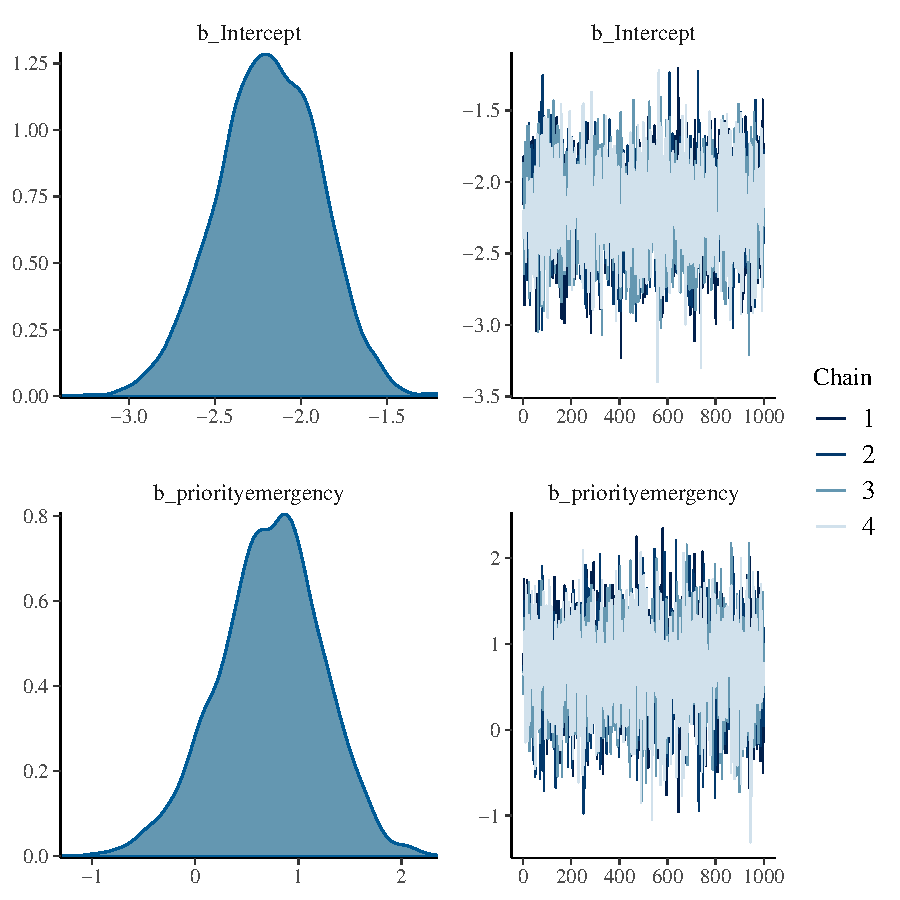
\includegraphics[width=\maxwidth]{prop-bayesprop2-1} }

\end{Schunk}

\begin{Schunk}
\begin{Sinput}
# Bring out posterior draws
w <- as.data.frame(f)
b0 <- w[, 'b_Intercept']
b1 <- w[, 'b_priorityemergency']
r  <- rbind(c(mean(b0), median(b0), pmode(b0)),
            c(mean(b1), median(b1), pmode(b1)),
            c(mean(exp(b1)), median(exp(b1)), pmode(exp(b1))))
colnames(r) <- c('Posterior Mean', 'Posterior Median', 'Posterior Mode')
rownames(r) <- c('b0', 'b1', 'OR')
round(r, 3)
\end{Sinput}
\begin{Soutput}
   Posterior Mean Posterior Median Posterior Mode
b0         -2.188           -2.184         -2.203
b1          0.724            0.748          0.865
OR          2.333            2.113          1.721
\end{Soutput}
\end{Schunk}

Because the prior on the OR is conservative, the Bayesian posterior mode for the OR is smaller than the frequentist maximum likelihood estimate of 2.87.  

Below notice how easy it is to do Bayesian inference on derived quantities p1 and p2 which are functions of b0 and b1.

\begin{Schunk}
\begin{Sinput}
# 0.95 credible interval for log odds ratio and odds ratio
quantile(b1, c(0.025, 0.975))
\end{Sinput}
\begin{Soutput}
     2.5%     97.5% 
-0.326236  1.656346 
\end{Soutput}
\begin{Sinput}
quantile(exp(b1), c(.025, 0.975))
\end{Sinput}
\begin{Soutput}
    2.5%    97.5% 
0.721635 5.240131 
\end{Soutput}
\begin{Sinput}
exp(quantile(b1,  c(0.025, 0.975)))
\end{Sinput}
\begin{Soutput}
     2.5%     97.5% 
0.7216349 5.2401303 
\end{Soutput}
\begin{Sinput}
# Posterior density of emergency:other odds ratio
plot(density(exp(b1)), xlab='OR', main='')
abline(v=c(1, pmode(exp(b1))), col=gray(0.85))
# Probability that OR > 1
P(exp(b1) > 1)
\end{Sinput}
\begin{Soutput}
[1] 0.91875
\end{Soutput}
\begin{Sinput}
# Probability it is > 1.5
P(exp(b1) > 1.5)
\end{Sinput}
\begin{Soutput}
[1] 0.74925
\end{Soutput}
\begin{Sinput}
# Probability that risk with emergency surgery exceeds that of
# non-emergency (same as P(OR > 1))
# plogis in R is 1/(1 + exp(-x))
P(plogis(b0 + b1) > plogis(b0))
\end{Sinput}
\begin{Soutput}
[1] 0.91875
\end{Soutput}
\begin{Sinput}
# Prob. that risk with emergency surgery elevated by more than 0.03
P(plogis(b0 + b1) > plogis(b0) + 0.03)
\end{Sinput}
\begin{Soutput}
[1] 0.8165
\end{Soutput}


\centerline{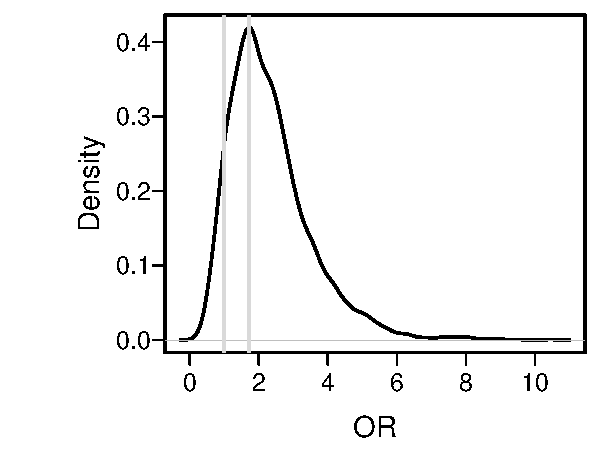
\includegraphics[width=\maxwidth]{prop-bayesprop4-1} }

\end{Schunk}

Even though the priors for the intercept and log odds ratio are independent, the connection of these two parameters in the data likelihood makes the posteriors dependent as shown with Spearman correlations of the posterior draws below.  Also get the correlation between evidence for the two probabilities.  These have correlated priors even though they are unconnected in the likelihood function.  Posteriors for $p_1$ and $p_2$ are less correlated than their priors.

\begin{Schunk}
\begin{Sinput}
cor(b0, b1, method='spearman')
\end{Sinput}
\begin{Soutput}
[1] -0.4439781
\end{Soutput}
\begin{Sinput}
cor(plogis(b0), plogis(b0 + b1), method='spearman')
\end{Sinput}
\begin{Soutput}
[1] 0.1385611
\end{Soutput}
\end{Schunk}


To demonstrate the effect of a skeptical prior:
\bi
\item Add random grouping to model as we did with the frequentist analysis
\item Make use of prior information that this variable is unlikely to be important
\item Put a prior on the log OR for this variable centered at zero with chance that the OR $> 1.25$ of only 0.05
\ei

\begin{Schunk}
\begin{Sinput}
normsolve(0, log(1.25), 0.05)
\end{Sinput}
\begin{Soutput}
[1] 0.1356616
\end{Soutput}
\begin{Sinput}
p <- c(prior(normal(-2.944, 1.216), class='Intercept'),
       prior(normal(0, 0.857),      class='b', coef='priorityemergency'),
       prior(normal(0, 0.136),      class='b', coef='random'))

f2 <- brm(death ~ priority + random, data=d, prior=p, family='bernoulli',
          seed=121, refresh=FALSE)
\end{Sinput}
\begin{Sinput}
f2
\end{Sinput}
\begin{Soutput}
 Family: bernoulli 
  Links: mu = logit 
Formula: death ~ priority + random 
   Data: d (Number of observations: 136) 
Samples: 4 chains, each with iter = 2000; warmup = 1000; thin = 1;
         total post-warmup samples = 4000

Population-Level Effects: 
                  Estimate Est.Error l-95% CI u-95% CI Rhat Bulk_ESS Tail_ESS
Intercept            -2.16      0.31    -2.82    -1.61 1.00     2804     2922
priorityemergency     0.71      0.50    -0.27     1.66 1.00     3614     3020
random               -0.06      0.13    -0.31     0.19 1.00     3879     3110

Samples were drawn using sampling(NUTS). For each parameter, Eff.Sample 
is a crude measure of effective sample size, and Rhat is the potential 
scale reduction factor on split chains (at convergence, Rhat = 1).
\end{Soutput}
\end{Schunk}

\bi
\item Effect of \co{random} is greatly discounted
\item Posterior mean priority effect and its credible interval is virtually the same as the model that excluded \co{random}
\ei

James Rae and Nils Reimer have written a nice tutorial on using the \R~\co{brms} package for binary logistic regression available at
\href{http://bit.ly/brms-lrm}{bit.ly/brms-lrm}

%% Usage: knitr slide

%
%### One sample/Paired: Modification of Student's sleep data ###%
%
%d1 <- sleep$extra[sleep$group==2] - sleep$extra[sleep$group==1]
%d1[1] <- d1[1] * -1

\chapter{Nonparametric Statistical Tests}\alabel{chap:nonpar}\ros{9}\katz{5.4}\bmovie{10}\ddisc{10}
\section{When to use non-parametric methods}
\bi
\item Short answer: Good default when $P$-values are needed and there are no covariates to adjust for
\item Nonparametric methods are those not requiring one to assume a
  certain distribution for the raw data
  \bi
  \item In contrast, parametric methods assume data come from some underlying distribution
  \item $t$-tests assume the data come form a Gaussian distribution
  \ei
\item Response variable ordinal or interval
\item For ordinal responses nonparametric methods are preferred
  because they assume no spacing between categories
\item No problem in using nonparametric tests on interval data
 \bi
 \item if normality holds, nonpar.\ test 0.95 efficient, i.e., has
   about the same power as the parametric test done on 0.95 of the
   observations\footnote{The large-sample efficiency of the Wilcoxon
     and Spearman tests compared to $t$ and $r$ tests is
     $\frac{3}{\pi} = 0.9549$.}
 \item if normality does not hold, nonpar.\ tests can be arbitrarily
   more efficient and powerful than the corresponding parametric test 
 \item an elegant and non-arbitrary way to deal with extreme values or
   outliers
 \item rank-based nonparametric tests give the analyst freedom from
   having to choose the correct transformation of the measurement (as
   long as the optimum transformation is monotonic)
 \ei
\item Nonparametric methods are robust, many parametric methods are
  not
 \bi
 \item Example: $t$-test comparing two sets of measurements\\
   1 2 3 4 5 6 7 8 9 10 \hfill vs.\ \hfill 7 8 9 10 11 12 13 14 15 16
   17 18 19 20\\
   means: 5.5 and 13.5, $P=0.000019$\\
   1 2 3 4 5 6 7 8 9 10 \hfill vs.\ \hfill 7 8 9 10 11 12 13 14 15 16
   17 18 19 20 \textbf{200}\\
   means: 5.5 and 25.9, $P=0.12$\\
   The SD is a particularly non-robust statistical estimator.
  \ei

\item Example: Fecal calprotectin being evaluated as a possible
  biomarker of disease severity (Figure \ref{fig:nonpar-calpro})
 \bi 
  \item Calprotectin has an upper detection limit
  \item Median can be calculated (mean cannot)
 \ei
\item If all you want is a $P$-value nonpar.\ tests are preferred
 \bi
 \item Especially if response is univariate and no need to adjust for
   covariates
 \ei
\item Pre-testing for normality and deciding nonparametric
  vs.\ parametric analysis is a bad idea
 \bi
 \item Tests for normality do not have a power of 1.0 and type I error
   of 0.0
 \item Leads to temptation, e.g., an investigator might ``forget'' to do the
   test of normality if the $t$-test is significant
 \item Doesn't acknowledge that nonparametric tests are very efficient
   even under normality
 \item Pre-testing for normality alters the type I error and confidence interval coverage
 \ei
\item A drawback is that nonpar.\ tests do not correspond to
  usual confidence limits for effects
 \bi
  \item E.g., a CL for the difference in 2 means may include zero whereas
  the Wilcoxon test yields $P=0.01$
  \item Point estimate that exactly corresponds to the Wilcoxon
    two-sample test is the Hodges-Lehman estimate of the location
    difference
  \bi
  \item median of all possible differences between a measurement from
    group 1 and a measurement from group 2
  \ei
 \ei
\item Nonparametric tests are often obtained by replacing the data
  with ranks across subjects and then doing the parametric test
\item Many nonpar.\ tests give the same $P$-value regardless of how
  the data are transformed; a careful choice of transformation (e.g.,
  log) must sometimes be used in the context of parametric tests
\item $P$-values computed using e.g.\ the $t$ distribution are quite
  accurate for nonparametric tests
\item In case of ties, midranks are used, e.g., if the raw data were
  105 120 120 121 the ranks would be 1 2.5 2.5 4

\begin{center}
\begin{tabular}{lll} \hline
Parametric Test & Nonparametric Counterpart & Semiparametric Model \\
                &                           & Counterpart \\ \hline
1-sample $t$    & Wilcoxon signed-rank & \\
2-sample $t$    & Wilcoxon 2-sample rank-sum & Proportional odds \\
$k$-sample ANOVA           & Kruskal-Wallis  & Proportional odds \\
Pearson $r$     & Spearman $\rho$ & \\ \hline
\end{tabular}\end{center}
\ei

\section{One Sample Test: Wilcoxon Signed-Rank} \ros{9.3}\katz{5.10.E}
\bi
\item Almost always used on paired data where the column of values
  represents differences (e.g., post-pre) or log ratios
\item The \emph{sign test} is the simplest test for the median
  difference being zero in the population
 \bi
 \item it just counts the number of positive differences after tossing
   out zero differences
 \item tests $H_{0}:$Prob$[x>0]=\frac{1}{2}$, i.e., that it is
   equally likely in the population to have a value below zero as it
   is to have a value above zero
 \item as it ignores magnitudes completely, the test is inefficient
 \ei
\item By contrast, with the much more powerful Wilcoxon signed rank one-sample test, ranks of absolute
  differences are given the sign of the original difference
\item Magnitudes of raw data matter more here than with the Wilcoxon
  2-sample test
\item Example: A crossover study in which the treatment order is  randomized \\
  Data arranged so that treatment A is in the first column, no matter which order treatment A was given


\begin{center}
\begin{tabular}{ccccc} \hline
A & B & B-A & Rank $|\mathrm{B-A}|$ & Signed Rank \\ \hline
5 & 6 & ~1 & 1.5 & ~1.5 \\
6 & 5 & -1 & 1.5 & -1.5 \\
4 & 9 & ~5 & 4.0 & ~4.0 \\
7 & 9 & ~2 & 3.0 & ~3.0 \\ \hline
\end{tabular}\end{center}

\item A good approximation to an exact $P$-value may be obtained by computing
\beq
z = \frac{\sum{SR_{i}}}{\sqrt{\sum{SR_{i}^{2}}}},
\eeq
where the signed rank for observation $i$ is $SR_{i}$.  This formula
already takes ties into account without using Rosner's messy Eq.\
9.5.  We look up $|z|$ against the normal distribution.  Here
$z=\frac{7}{\sqrt{29.5}}=1.29$ and and the 2-tailed $P$-value is given below.
\begin{Schunk}
\begin{Sinput}
sr <- c(1.5, -1.5, 4, 3)
z <- sum(sr) / sqrt(sum(sr ^ 2))
pval <- 2 * (1 - pnorm(abs(z)))
c(z=z, pval=pval)
\end{Sinput}
\begin{Soutput}
        z      pval 
1.2888045 0.1974661 
\end{Soutput}
\end{Schunk}
\item If all differences are positive or all are negative, the exact
  2-tailed $P$-value is $\frac{1}{2^{n-1}}$
 \bi
 \item implies that $n$ must exceed 5 for any possibility of
   significance at the $\alpha=0.05$ level for a 2-tailed test
 \ei
\ei

\subsection{One sample/Paired Test Example}

\bi
\item Sleep Dataset
\bi
\item Compare the effects of two soporific drugs.
\item Each subject receives placebo, Drug 1, and Drug 2
\item Study question: Is Drug 1 or Drug 2 more effective at increasing sleep?
%\item Side comment: why did the investigators believe that the original 4-level ordinal outcome was so defective that it needed to be %transformed in an information-losing way?
\item Dependent variable: Difference in hours of sleep comparing Drug 2 to Drug 1
\item $H_0:$ For any given subject, the difference in hours of sleep is equally likely to be positive or negative
\item See P.~\pageref{sleeppaired} for a parametric test on these data
\ei
\ei
%\clearpage
\begin{table}[!hbp]
 \begin{center}
 \begin{tabular}{lrrrcc}\hline\hline
Subject & Drug 1 & Drug 2 & \color{red}Diff (2-1) & Sign & Rank \\ \hline
1  &$ 0.7$&$ 1.9$&$\color{red}1.2$&+&$3$\\
2  &$-1.6$&$ 0.8$&$\color{red}2.4$&+&$8$\\
3  &$-0.2$&$ 1.1$&$\color{red}1.3$&+&$4.5$\\
4  &$-1.2$&$ 0.1$&$\color{red}1.3$&+&$4.5$\\
5  &$-0.1$&$-0.1$&$\color{red}0.0$&NA&\\
6  &$ 3.4$&$ 4.4$&$\color{red}1.0$&+&$2$\\
7  &$ 3.7$&$ 5.5$&$\color{red}1.8$&+&$7$\\
8  &$ 0.8$&$ 1.6$&$\color{red}0.8$&+&$1$\\
9  &$ 0.0$&$ 4.6$&$\color{red}4.6$&+&$9$\\
10 &$ 2.0$&$ 3.4$&$\color{red}1.4$&+&$6$\\
\hline
\end{tabular}
\caption{Hours of extra sleep on drugs 1 and 2, differences, signs and
  signed ranks of sleep study data}
\end{center}
\end{table}
\begin{Schunk}
\begin{Sinput}
drug1 <- c(.7, -1.6, -.2, -1.2, -.1, 3.4, 3.7, .8, 0, 2)
drug2 <- c(1.9, .8, 1.1, .1, -.1, 4.4, 5.5, 1.6, 4.6, 3.4)
wilcox.test(drug2, drug1, paired=TRUE)
\end{Sinput}
\begin{Soutput}

	Wilcoxon signed rank test with continuity correction

data:  drug2 and drug1
V = 45, p-value = 0.009091
alternative hypothesis: true location shift is not equal to 0
\end{Soutput}
\begin{Sinput}
wilcox.test(drug2 - drug1)
\end{Sinput}
\begin{Soutput}

	Wilcoxon signed rank test with continuity correction

data:  drug2 - drug1
V = 45, p-value = 0.009091
alternative hypothesis: true location is not equal to 0
\end{Soutput}
\begin{Sinput}
wilcox.test(drug2 - drug1, correct=FALSE)
\end{Sinput}
\begin{Soutput}

	Wilcoxon signed rank test

data:  drug2 - drug1
V = 45, p-value = 0.007632
alternative hypothesis: true location is not equal to 0
\end{Soutput}
\begin{Sinput}
sr <- c(3, 8, 4.5, 4.5, 0, 2, 7, 1, 9, 6)
z <- sum(sr) / sqrt(sum(sr ^ 2))
c(z=z, pval=2 * (1 - pnorm(abs(z))))
\end{Sinput}
\begin{Soutput}
          z        pval 
2.667911250 0.007632442 
\end{Soutput}
\begin{Sinput}
d <- data.frame(Drug=c(rep('Drug 1', 10), rep('Drug 2', 10),
                  rep('Difference', 10)),
                extra=c(drug1, drug2, drug2 - drug1))
\end{Sinput}
\end{Schunk}
\bi 
\item Interpretation: Reject $H_0$, Drug 2 increases sleep by the same hours as Drug 1 ($p = 0.008$)
\item Could also perform sign test on sleep data
 \bi
 \item If drugs are equally effective, should have same number of `+' and '-'
 \item Observed data: 0 `-', 9 `+', throw out 1 `no change' 
 \item Sign test (2-sided) $P$-value: Probability of observing 9 of 9
   + or 9 of 9 -
 \item $p = 0.004$, so evidence against $H_0$
 \ei
\ei
\begin{Schunk}
\begin{Sinput}
2 * (1 / 2) ^ 9    # 2 * to make it two-tailed
\end{Sinput}
\begin{Soutput}
[1] 0.00390625
\end{Soutput}
\end{Schunk}

\bi
\item The signed rank test assumes that the distribution of differences is
  symmetric
\item It tests whether the median difference is zero
\item Also tests that the mean is zero
\item In general it tests that, for two randomly chosen observations
  $i$ and $j$ with values (differences) $x_i$ and $x_j$, that the
  probability that $x_{i}+x_{j} > 0$ is $\frac{1}{2}$
\item The estimator that corresponds exactly to the test in all
  situations is the pseudomedian, the median of all possible pairwise
  averages of $x_i$ and $x_j$, so one could say that the signed rank
  test tests $H_{0}$: pseudomedian=0
\item The value $\frac{\overline{SR}}{n+1}-\frac{1}{2}$ estimates the
  probability that two randomly chosen observations have a positive
  sum, where $\overline{SR}$ is the mean of the column of signed ranks
\item To test $H_{0}:\eta=\eta_{0}$, where $\eta$ is the population median
  (not a difference) and $\eta_{0}$ is some constant, we create the $n$ values
  $x_{i} - \eta_{0}$ and feed those to the signed rank test, assuming
  the distribution is symmetric
\item When all nonzero values are of the same sign, the test reduces
  to the \emph{sign test} and the 2-tailed $P$-value is
  $(\frac{1}{2})^{n-1}$ where $n$ is the number of nonzero values
\ei

Test whether the continuity correction makes $P$-values closer to the
exact calculation\footnote{The exact $P$-value is available only when
  there are no ties.}, and compare to our simple formula.
\begin{Schunk}
\begin{Sinput}
# Assume we are already starting with signed ranks as x
wsr <- function(x, ...) wilcox.test(x, ...)$p.value
sim <- function(x) {
  z <- sum(x) / sqrt(sum(x ^ 2))
  2 * (1 - pnorm(abs(z))) }
all <- function(x) round(c(
  continuity=wsr(x, correct=TRUE, exact=FALSE),
  nocontinuity=wsr(x, correct=FALSE, exact=FALSE),
  exact=wsr(x, exact=TRUE),
  simple=sim(x)), 4)
all(1:4)
\end{Sinput}
\begin{Soutput}
  continuity nocontinuity        exact       simple 
      0.1003       0.0679       0.1250       0.0679 
\end{Soutput}
\begin{Sinput}
all(c(-1, 2 : 4))
\end{Sinput}
\begin{Soutput}
  continuity nocontinuity        exact       simple 
      0.2012       0.1441       0.2500       0.1441 
\end{Soutput}
\begin{Sinput}
all(c(-2, c(1, 3, 4)))
\end{Sinput}
\begin{Soutput}
  continuity nocontinuity        exact       simple 
      0.3613       0.2733       0.3750       0.2733 
\end{Soutput}
\begin{Sinput}
all(c(-1, -2, 3 : 5))
\end{Sinput}
\begin{Soutput}
  continuity nocontinuity        exact       simple 
      0.2807       0.2249       0.3125       0.2249 
\end{Soutput}
\begin{Sinput}
all(c(-5, -1, 2, 3, 4, 6))
\end{Sinput}
\begin{Soutput}
  continuity nocontinuity        exact       simple 
      0.4017       0.3454       0.4375       0.3454 
\end{Soutput}
\end{Schunk}
From these examples the guidance is to:
\bi
\item Use the exact calculation if there are no ties
\item Otherwise use the continuity correction (i.e., the default in
  \Co{wilcox.test}) unlike the recommendation for the Pearson $\chi^2$ test
\ei

\section{Two Sample Test: Wilcoxon--Mann--Whitney} \ros{9.4}\katz{5.5.B}
\bi
\item The Wilcoxon--Mann--Whitney (WMW) 2-sample rank sum test is for
  testing for equality of central tendency of two distributions (for
  unpaired data)
\item Ranking is done by combining the two samples and ignoring which
  sample each observation came from
\item Example:

\begin{center}\begin{tabular}{lrrrr} \hline
Females           & 120 & 118 & 121 & 119 \\
Males             & 124 & 120 & 133 &     \\ \hline
Ranks for Females & 3.5 & ~~1 & ~~5 & ~~2 \\
Ranks for Males   & ~~6 & 3.5 & ~~7 &     \\ \hline
\end{tabular}\end{center}

\item Doing a 2-sample $t$-test using these ranks as if they were raw
  data and computing the $P$-value against 4+3-2=5 d.f.\ will work
  quite well
\item Some statistical packages compute $P$-values exactly (especially
  if there are no ties)
\item Loosely speaking the WMW test tests whether the population
  medians of the two groups are the same
\item More accurately and more generally, it tests whether
  observations in one population tend to be larger than observations
  in the other
\item Letting $x_1$ and $x_2$ respectively be randomly chosen
  observations from populations one and two, WMW tests
  $H_{0}:c=\frac{1}{2}$, where $c=$Prob$[x_{1} > x_{2}]$
\item The $c$ index (\emph{concordance probability}) may be estimated
  by computing
\beq
c = \frac{\bar{R}-\frac{n_{1}+1}{2}}{n_{2}},
\eeq
where $\bar{R}$ is the mean of the ranks in group 1; \\
For the above data $\bar{R} = 2.875$ and
$c=\frac{2.875-2.5}{3}=0.125$, so we estimate that the probability is
0.125 that a randomly chosen female has a value greater than a randomly
chosen male.
\item In diagnostic studies where $x$ is the continuous result of a
  medical test and the grouping variable is diseased vs.\ non-diseased,
  $c$ is the area under the receiver operating characteristic (ROC) curve
\item Test still has the ``probability of ordering'' interpretation
  when the variances of the two samples are markedly different, but it
  no longer tests anything like the difference in population medians
\ei
If there is no overlap between measurements from group 1 and those
from group 2, the exact 2-sided $P$-value for the Wilcoxon test is $2
/ \frac{n!}{n_{1}! n_{2}!}$.  If $n_{1}=n_{2}$, $n_{1}$ must be $\geq
4$ to obtain $P < 0.05$ (in this case $P = 0.029$). 
% Thanks: Rameela and Bill
%If R1 denotes the rank sum of the group with sample size m, then the
%smallest possible value of R1 is the sum of the m smallest ranks 1 + 2 +
%... m = m*(m+1)/2. The probability of this value is 1/[(m+n)Cm] -- C
%implies choose.

\subsection{Two Sample WMW example}\label{sec:calprotectin}
\bi 
\item Fecal calprotectin being evaluated as a possible biomarker of
  disease severity 
\item Calprotectin measured in 26 subjects, 8 observed to have no/mild
  activity by endoscopy 
\item Calprotectin has upper detection limit at 2500 units
 \bi 
 \item A type of missing data, but need to keep in analysis
 \ei
\item Study question: Are calprotectin levels different in subjects
  with no or mild activity compared to subjects with moderate or
  severe activity? 
\item Statement of the null hypothesis
 \bi 
 \item $H_0:$ Populations with no/mild activity have the same
   distribution of calprotectin as populations with moderate/severe
   activity 
 \item $H_0: c = \frac{1}{2}$
 \ei
\ei
\begin{Schunk}
\begin{Sinput}
#Fecal Calprotectin: 2500 is above detection limit
calpro <- c(2500, 244, 2500, 726, 86, 2500, 61, 392, 2500, 114, 1226,
            2500, 168, 910, 627, 2500, 781, 57, 483, 30, 925, 1027,
            2500, 2500, 38, 18)

# Endoscopy score: 1 = No/Mild, 2=Mod/Severe Disease
# Would have been far better to code dose as 4 ordinal levels
endo <- c(2, 1, 2, 2, 2, 1, 1, 2, 2, 1, 2, 2, 1, 2, 2, 2, 2, 1, 2,
          2, 2, 2, 2, 2, 1, 1)
endo <- factor(endo, 1 : 2,
               c("No or Mild Activity", "Moderate or Severe Activity"))
require(ggplot2)   # Fig. (*\ref{fig:nonpar-calpro}*)
ggplot(data.frame(endo, calpro), aes(y=calpro, x=endo)) +
  geom_boxplot(color='lightblue', alpha=.85, width=.4) +
  geom_dotplot(binaxis='y', stackdir='center', position='dodge') +
    xlab('') + ylab('Fecal Calprotectin') + coord_flip() +
      geom_hline(aes(yintercept=2500, col=I('red')), linetype='dotted')
\end{Sinput}
\begin{Sinput}
wilcox.test(calpro ~ endo)
\end{Sinput}
\begin{Soutput}

	Wilcoxon rank sum test with continuity correction

data:  calpro by endo
W = 23.5, p-value = 0.006814
alternative hypothesis: true location shift is not equal to 0
\end{Soutput}
\begin{figure}[htbp]

\centerline{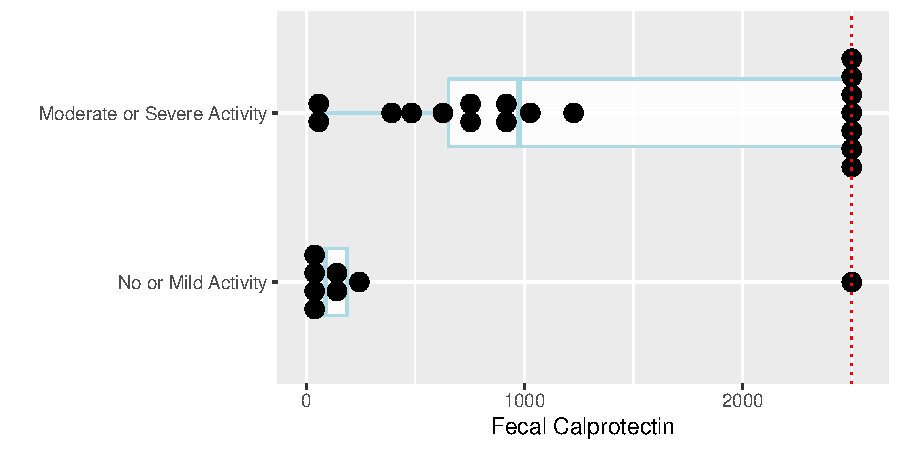
\includegraphics[width=\maxwidth]{nonpar-calpro-1} }

\caption[Fecal calprotectin by severity]{Fecal calprotectin by endoscopy severity rating. Red dotted line is the detection limit.  Ordinal disease categories should not have been combined.}\label{fig:nonpar-calpro}
\end{figure}
\end{Schunk}
% See http://docs.ggplot2.org/0.9.3/geom_dotplot.html
The following plots the ranks that are used in the
Wilcoxon-Mann-Whitney two-sample rank sum test.
\begin{Schunk}
\begin{Sinput}
ggplot(data.frame(endo, calpro), aes(y=rank(calpro), x=endo)) + #Fig (*\ref{fig:nonpar-calpror}*)
  geom_dotplot(binaxis='y', stackdir='center', position='dodge') +
    xlab('') + ylab('Rank of Fecal Calprotectin') + coord_flip()
\end{Sinput}
\begin{figure}[htbp]

\centerline{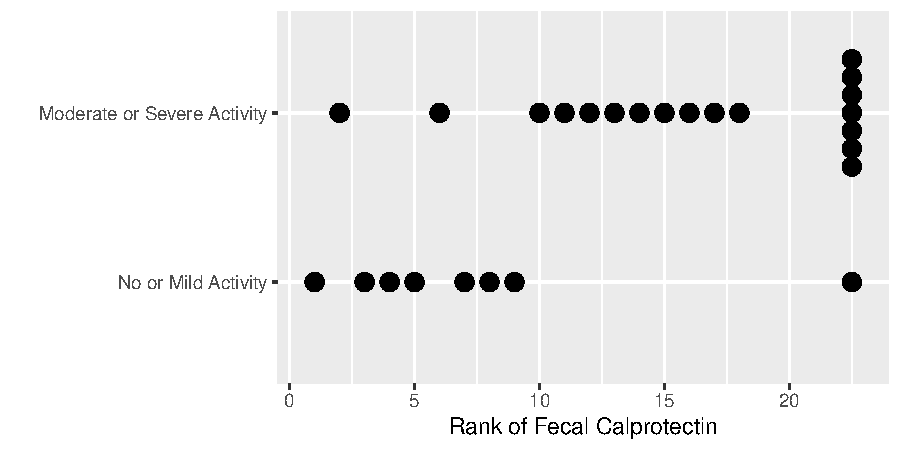
\includegraphics[width=\maxwidth]{nonpar-calpror-1} }

\caption[Ranks of calprotectin]{Ranks of calprotectin}\label{fig:nonpar-calpror}
\end{figure}
\end{Schunk}
\bi
\item Test statistic $W$ equals the sum of the ranks in the no/mild group minus $n_1 * (n_1 + 1) / 2$, where $n_1$ is the number of subjects in then no/mild sample
\item $W = 59.5 - \frac{8*9}{2} = 23.5$
\item A common (but loose) interpretation: People with moderate/severe activity have higher \textit{median} fecal calprotectin levels than people with no/mild activity ($p = 0.007$).
\item Better: remove \textit{median} and supplement with the $c$-index
  (concordance probability) or Somers' $D_{xy}$ rank correlation
  between calprotectin and endoscopy status.  The code for the \R\
  \Co{somers2} function shows how the concordance probability is
  computed from the mean of the ranks in one of the two groups.
\ei
\begin{Schunk}
\begin{Sinput}
require(Hmisc)
# Convert endo to a binary variable
somers2(calpro, endo=='Moderate or Severe Activity')
\end{Sinput}
\begin{Soutput}
         C        Dxy          n    Missing 
 0.8368056  0.6736111 26.0000000  0.0000000 
\end{Soutput}
\end{Schunk}
If you type \Co{somers2} to list the code for the function you will
see that the $c$-index is tightly related to the Wilcoxon test when
you see this code:
\begin{Schunk}
\begin{Sinput}
mean.rank <- mean(rank(x)[y == 1])
c.index <- (mean.rank - (n1 + 1)/2) / (n - n1)
\end{Sinput}
\end{Schunk}

\subsection{Point and Interval Estimates for Wilcoxon Two-Sample Comparison}
As mentioned earlier, the effect estimate that is exactly consistent
with the Wilcoxon two-sample test is the robust Hodges-Lehman estimator---the
median of all possible differences between a measurement from group 1
and a measurement from group 2.  There is a confidence interval for
this estimator.
\bi
\item Assume data come from distributions with same shape and differ only in location
\item Consider a sample of 4 males and 3 females
\item Difference in sample medians is 124 - 119.5 = 4.5
\item Consider all possible differences between sample 1 and sample 2
\ei
\begin{center}\begin{tabular}{l|cccc} \hline \hline \alabel{pg:nonpar-mf}
 & \multicolumn{4}{c}{Female} \\
Male & 120 & 118 & 121 & 119 \\ \hline
124 & 4 & 6 & 3 & 5 \\ 
120 & 0 & 2 & -1 & 1 \\
133 & 13 & 15 & 12 & 14 \\ \hline
\end{tabular}\end{center}
\bi
\item Hodges-Lehman estimate of the sex effect: median of the 12
  differences = 4.5
\item In this case equaled difference in sample medians just by coincidence
\ei
\begin{Schunk}
\begin{Sinput}
female <- c(120, 118, 121, 119)
male   <- c(124, 120, 133)
differences <- outer(male, female, '-')
differences
\end{Sinput}
\begin{Soutput}
     [,1] [,2] [,3] [,4]
[1,]    4    6    3    5
[2,]    0    2   -1    1
[3,]   13   15   12   14
\end{Soutput}
\begin{Sinput}
median(differences)
\end{Sinput}
\begin{Soutput}
[1] 4.5
\end{Soutput}
\begin{Sinput}
# Can't figure out how difference in location is computed below
# It's not the Hodges-Lehman estimate
wilcox.test(male, female, conf.int=TRUE)
\end{Sinput}
\begin{Soutput}

	Wilcoxon rank sum test with continuity correction

data:  male and female
W = 10.5, p-value = 0.1536
alternative hypothesis: true location shift is not equal to 0
95 percent confidence interval:
 -1 15
sample estimates:
difference in location 
              4.791134 
\end{Soutput}
\end{Schunk}
In general, $1 - \alpha$ confidence intervals are the set of values that if
hypothesized to be the true location parameter would not be rejected
at the $\alpha$ level.  \Co{wilcox.test} computes the location shift
by solving for the hypothesized value that yields $P=1.0$ instead of
the more proper median of all differences.  Look into this further by
plotting the $P$-value as a function of the hypothesized value.
\begin{Schunk}
\begin{Sinput}
dif  <- seq(-3, 15, by=.1)
n    <- length(dif)
pval <- numeric(n)
for(i in 1 : n) pval[i] <- wilcox.test(male - dif[i], female)$p.value
\end{Sinput}
\begin{Sinput}
ggplot(data.frame(dif, pval), aes(x=dif, y=pval)) +
  geom_step() +
  geom_hline(yintercept=.05, col='red', linetype='dotted') +
  geom_vline(xintercept=c(4.5, 4.791, -1, 15), col='red', linetype='dotted') +
  xlab('Difference') + ylab('P-value')
\end{Sinput}
\begin{figure}[htbp]

\centerline{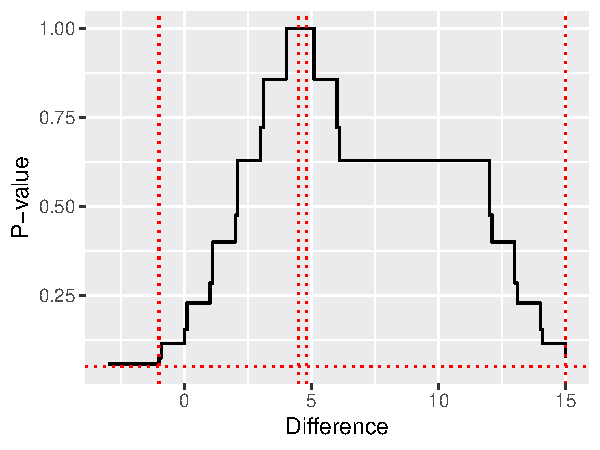
\includegraphics[width=\maxwidth]{nonpar-checkhl-1} }

\caption[Wilcoxon $P$-value vs.\ hypothesized difference.]{Wilcoxon $P$-value vs.\ hypothesized male-female difference.  Horizontal line is $P=0.05$.  Vertical lines from left to right are the lower 0.95 confidence limit from \Co{wilcox.test}, the median difference, the Hodges-Lehman estimator as computed by \Co{wilcox.test}, and the upper 0.95 confidence limit from \Co{wilcox.test}.}\label{fig:nonpar-checkhl}
\end{figure}
\end{Schunk}
See Section~\ref{sec:nonpar-clmed} for a more approximate confidence interval.

\section{Confidence Intervals for Medians and Their Differences} \altman{36-43}\alabel{sec:nonpar-clmed}
\bi 
\item Confidence intervals for the median (one sample)
\bi 
\item Table 18.4 (Altman) gives the ranks of the observations to be
  used to give approximate confidence intervals for the median 
\item e.g., if $n = 12$, the $3^\textrm{rd}$ and $10^\textrm{th}$
  largest values give a $0.961$ confidence interval 
\item For larger sample sizes, the lower ranked value ($r$) and upper
  ranked value ($s$) to select for an approximate $0.95$ confidence
  interval for the population median is 
\beq
r = \frac{n}{2} - 1.96*\frac{\sqrt{n}}{2} \hspace{.4cm}\textrm{and}
\hspace{.4cm} s = 1 + \frac{n}{2} + 1.96*\frac{\sqrt{n}}{2} 
\eeq
\item e.g., if $n = 100$ then $r = 40.2$ and $s = 60.8$, so we would pick the $40^\textrm{th}$ and $61^\textrm{st}$ largest values from the sample to specify a $0.95$ confidence interval for the population median
\item For exact confidence interval for the median see\\
  \href{https://stats.stackexchange.com/questions/186957}{stats.stackexchange.com/questions/186957}, which
  also discusses why there is no exact nonparametric confidence
  interval for the mean.  Let's get the exact order statistics that result in an exact confidence interval for the median:
\begin{Schunk}
\begin{Sinput}
# Exact CI for median from DescTools package SignTest.default
# See also ttp://www.stat.umn.edu/geyer/old03/5102/notes/rank.pdf,
# http://de.scribd.com/doc/75941305/Confidence-Interval-for-Median-Based-on-Sign-Test
cimed <- function(x, alpha=0.05, na.rm=FALSE) {
  if(na.rm) x <- x[! is.na(x)]
  n <- length(x)
  k <- qbinom(p=alpha / 2, size=n, prob=0.5, lower.tail=TRUE)
  ## Actual CL: 1 - 2 * pbinom(k - 1, size=n, prob=0.5) >= 1 - alpha
  sort(x)[c(k, n - k + 1)]
}
cimed(1 : 100)
\end{Sinput}
\begin{Soutput}
[1] 40 61
\end{Soutput}
\end{Schunk}
For $n=100$ we see that the approximate interval happened to be exact.
\ei
\item Confidence intervals for the difference in two medians (two samples)
\bi
\item We don't have a nonparametric interval for this
\item Instead get Hodges-Lehman estimate
\item Assume data come from distributions with same shape and differ only in location
\item Considers all possible differences between sample 1 and sample 2
  using male-female data on P.~\pageref{pg:nonpar-mf}
\item An estimate of the median difference (males - females) is the median of these 12 differences, with the $3^\textrm{rd}$ and $10^\textrm{th}$ largest values giving an (approximate) 0.95 CI
\item Median estimate = 4.5, 0.95 CI = [1, 13]
\item Specific formulas found in Altman, pages 40-41
\ei
\item Bootstrap \altman{159-163}
\bi
\item General method, not just for medians
\item Non-parametric, does not assume symmetry (but may not be accurate)
\item Iterative method that repeatedly samples from the original data
\item Algorithm for creating a $0.95$ CI for the difference in two medians
\begin{enumerate}
\item Sample \textit{with replacement} from sample 1 and sample 2
\item Calculate the difference in medians, save result
\item Repeat Steps 1 and 2 1000 times
\end{enumerate}
\item A (naive) $0.95$ CI is given by the $25^\textrm{th}$ and $975^\textrm{th}$ largest values of your $1000$ median differences
\item For the male/female data, median estimate = 4.5, 0.95 CI = [-0.5, 14.5], which agrees with the conclusion from a WMW rank sum test ($p = 0.15$).  Note that the more accurate CI for the Hodges-Lehman estimate of $[-1, 15]$ was given earlier (output of \co{wilcox.test}).
\ei
\ei
\begin{Schunk}
\begin{Sinput}
diffs <- numeric(1000)
set.seed(13)
for(i in 1 : 1000) diffs[i] <-
  median(sample(male, replace=TRUE)) - median(sample(female, replace=TRUE))
ggplot(data.frame(diffs), aes(x=diffs)) + xlab('Differences in Medians') +
  geom_histogram(bin_widith=.01, color='blue', fill='white')
\end{Sinput}
\begin{Sinput}
quantile(diffs, c(0.025, 0.975))
\end{Sinput}
\begin{Soutput}
 2.5% 97.5% 
 -0.5  14.5 
\end{Soutput}


\centerline{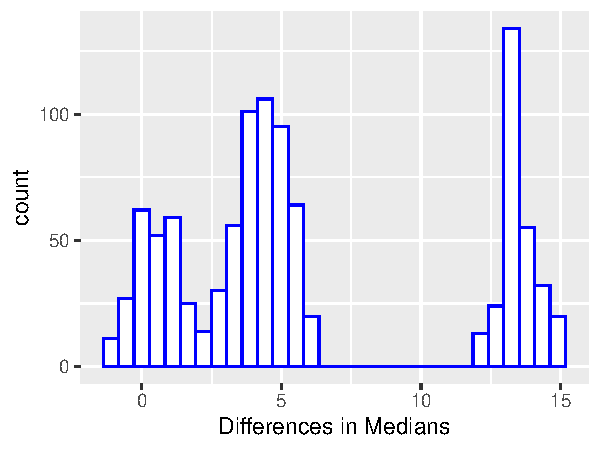
\includegraphics[width=\maxwidth]{nonpar-diffmedboot-1} }

\end{Schunk}
But recall that the Wilcoxon test does not really test the difference
in medians but rather the median of all differences.

\section{Strategy}
\bi
\item Don't assess normality of data
\item Use nonparametric test in any case, to get $P$-values
\item Use nonparametric confidence intervals for means and
  medians\footnote{A good nonparametric confidence for a population
    mean that does not even assume a symmetric distribution can be
    obtained from the bootstrap simulation procedure.}
  which will be more in conformance to what the nonpar.\ test is
  testing
\item To obtain nonparametric confidence limits for means and
  differences in means, the bootstrap percentile method may easily be
  used and it does not assume symmetry of the data distribution
\ei

\section{Generalization of the Wilcoxon/Kruskal-Wallis Test}\bmovie{11}\ddisc{11}
\bi
\item Proportional odds (PO) ordinal logistic model
\item Contains Wilcoxon 2-sample and Kruskal-Wallis tests as special cases
 \bi
 \item numerator of the score test for the PO model, when there is only the grouping variable in the model, is exactly the Wilcoxon statistic
 \ei
\item Special case of PO model is the ordinary binary logistic model
\item Advantages over nonparametric tests:
 \bi
 \item can adjust for covariates
 \item more accurate $P$-values even with extreme number of tied values
 \item provides a framework for consistent pairwise comparisons\footnote{When using the Kruskal-Wallis test followed by pairwise Wilcoxon tests, these pairwise tests can be inconsistent with each other, because they re-rank the data based only on two groups, destroying the transitivity property, e.g.\ treatment A can be better than B which is better than C but C is better than A.}
 \item provides estimates of means, quantiles, and exceedance probabilities
 \item sets the stage for a Bayesian PO model, so can get a Bayesian Wilcoxon test
 \ei
\item Other ordinal response models are available, e.g., Cox proportional hazards model
\item These models are \emph{semiparametric models}
 \bi
 \item parametric in additivity and linearity (by default) assumptions
 \item nonparametric in not assuming a distribution for the response variable
 \ei
\item Like nonparametric tests, $P$-values are unaffected by monotonic transformations of $Y$
\item If the response variable $Y$ has $k$ distinct values $y_1, y_2, \dots, y_k$ in the sample, semiparametric models have $k-1$ intercepts
\item Binary logistic model deals with prob.\ of only one event ($Y=1$ vs.\ $Y=0$)
\item For ordinal $Y$ there are $k-1$ events
\item Model these as cumulative probabilities to make use of ordering of $Y$ values
\item Model: $P(Y \geq y | X) = \frac{1}{1 + \exp[-(\alpha_y + \beta_1 x_1 + \beta_2 x_2 + \dots)]}$
\item $\alpha_y$ is the $j^{\textrm{th}}$ intercept when $y = y_{j+1}$, e.g. the first intercept corresponds to the second lowest distinct $Y$ value $y_2$
\item Special case: 2-group problem: $P(Y \geq y | \textrm{group}) = \frac{1}{1 + \exp[-(\alpha_y + \beta_1[\textrm{group B}])]}$
 \bi
 \item $\exp(\beta_1)$ is the ratio of odds that $Y \geq y$ in group B vs.\ $Y \geq y$ in group A, for all $y > y_1$ 
 \item as before $[x]$ is the 0-1 indicator variable for $x$ being true
 \item $\beta_1 > 0 \rightarrow Y$ values higher in group B
 \item $k=2 \rightarrow$ model is the binary logistic model (where we take $\alpha_1 = \beta_0$)
 \ei
\item These intercepts $\alpha_1, \alpha_2, \dots, \alpha_{k-1}$ encode the entire empirical distribution of $Y$ for one of the groups
 \bi
 \item $\rightarrow$ the model assumes nothing about the $Y$ distribution
 \item it only assumes how the distribution of $Y$ for one type of subject is connected to the distribution for another type of subject
 \item PO model for a two-group problem assumes that the logit of the two cumulative distribution functions are parallel
 \item if PO doesn't hold, PO model may still be better than alternatives
 \item PO is also what the Wilcoxon/Kruskal-Wallis test assumes to have optimal power
 \item don't need an $\alpha$ for the lowest observed $Y$ value since $P(Y \geq \textrm{minimum } Y) = 1$
 \ei
\item \R\ \co{rms} package \co{orm} function fits the PO model\footnote{\co{orm} also fits other models using link functions other than the logit.} and is especially made for continuous $Y$, with fast run times for up to 6000 intercepts
\ei

\subsection{Kruskal-Wallis Test}
\bi
\item Notice we haven't described rank ANOVA---the Kruskal-Wallis test
\item Don't need it; just form a PO model with more than one indicator variable
\item E.g., to test for any differences among four groups A B C D form 3 indicator variables for B C D and let A be the reference cell that corresponds to the $\alpha$ intercepts
 \bi
 \item model is logit$P(Y \geq y | \textrm{group}) = \alpha_y + \beta_1 [B] + \beta_2 [C] + \beta_3 [D]$
 \ei
\item Use the likelihood ratio $\chi^2$ test from this model to test the global null hypothesis A=B=C=D with 3 d.f.
\item Solves the transitivity problem mentioned earlier
\item Can obtain consistent pairwise comparisons by forming odds ratios for any comparison
 \bi
 \item e.g. C:A comparison will use $\exp(\hat{\beta_{2}})$
 \item C:B comparison OR: $\exp(\hat{\beta_{2}} - \hat{\beta_{1}})$
 \ei
\item As before can convert the ORs to differences in medians/means because unlike the original nonparametric tests, the PO model can be used to obtain many types of predictions\footnote{The predicted mean for a set of covariate settings is obtained by using all the intercepts and $\beta$s to get exceedance probabilities for $Y \geq y$, taking successive differences in those probabilities to get cell probabilities that $Y=y$, then multiplying cell probabilities by the $y$ value attached to them, and summing.  This is the formula for the mean for a discrete distribution.}
\item Illustrate this by a non-PO example, checking to see how well the PO model can recover the sample means when assuming (the slightly incorrect) PO
\item Take 4 samples from normal distributions with the same variances but different means
\item Also show how to compare two of the samples without re-ranking the data as inconsistent Wilcoxon tests would do
\ei

\begin{Sinput}
set.seed(1)
group <- rep(c('A','B','C','D'), 100)
y <- rnorm(400, 100, 15) + 10*(group == 'B') + 20*(group=='C') + 30*(group=='D')
require(rms)
options(prType='latex')
dd <- datadist(group, y); options(datadist='dd')
f <- orm(y ~ group)
f    # use LR chi-square test as replacement for Kruskal-Wallis
\end{Sinput}

 \centerline{\textbf{Logistic (Proportional Odds) Ordinal Regression Model}}
 
 \begin{verbatim}
 orm(formula = y ~ group)
 \end{verbatim}
 
 {\fontfamily{phv}\selectfont \begin{center}\begin{tabular}{|c|c|c|c|}\hline
&Model Likelihood&Discrimination&Rank Discrim.\\
&Ratio Test& Indexes&Indexes\\\hline
Obs~\hfill 400&LR $\chi^{2}$~\hfill 193.31&$R^{2}$~\hfill 0.383&$\rho$~\hfill 0.633\\
Distinct $Y$~\hfill 400&d.f.~\hfill 3&$g$~\hfill 1.532&\\
$Y_{0.5}$~\hfill 115.0935&Pr$(>\chi^{2})$~\hfill \textless 0.0001&$g_{r}$~\hfill 4.626&\\
$\max|\frac{\partial\log L}{\partial \beta}|$~\hfill $2\!\times\!10^{-6}$&Score $\chi^{2}$~\hfill 193.21&$|\overline{\mathrm{Pr}(Y\geq Y_{0.5})-\frac{1}{2}}|$~\hfill 0.256&\\
&Pr$(>\chi^{2})$~\hfill \textless 0.0001&&\\
\hline
\end{tabular}
\end{center}}
 
 %latex.default(U, file = "", first.hline.double = FALSE, table = FALSE,     longtable = TRUE, lines.page = lines.page, col.just = rep("r",         ncol(U)), rowlabel = "", already.math.col.names = TRUE,     append = TRUE)%
 \setlongtables\begin{longtable}{lrrrr}\hline
 \multicolumn{1}{l}{}&\multicolumn{1}{c}{$\hat{\beta}$}&\multicolumn{1}{c}{S.E.}&\multicolumn{1}{c}{Wald $Z$}&\multicolumn{1}{c}{Pr$(>|Z|)$}\tabularnewline
 \hline
 \endhead
 \hline
 \endfoot
 group=B&~1.4221~&~0.2579~& 5.51&\textless 0.0001\tabularnewline
 group=C&~2.6624~&~0.2762~& 9.64&\textless 0.0001\tabularnewline
 group=D&~3.6606~&~0.2925~&12.52&\textless 0.0001\tabularnewline
 \hline
 \end{longtable}
 \addtocounter{table}{-1}

\begin{Schunk}
\begin{Sinput}
# Derive R function to use all intercepts and betas to compute predicted means
M <- Mean(f)
Predict(f, group, fun=M)
\end{Sinput}
\begin{Soutput}
  group      yhat     lower    upper
1     A  99.32328  95.87128 102.8162
2     B 111.21326 108.05575 114.3752
3     C 121.63880 118.56543 124.6699
4     D 129.70290 126.48067 132.8164

Response variable (y):  

Limits are 0.95 confidence limits
\end{Soutput}
\begin{Sinput}
# Compare with sample means
summarize(y, group, smean.cl.normal)
\end{Sinput}
\begin{Soutput}
  group         y     Lower    Upper
1     A  98.72953  95.81508 101.6440
2     B 111.69464 108.61130 114.7780
3     C 121.80841 118.93036 124.6865
4     D 130.05275 127.40318 132.7023
\end{Soutput}
\begin{Sinput}
# Compare B and C
k <- contrast(f, list(group='C'), list(group='B'))
k
\end{Sinput}
\begin{Soutput}
   Contrast      S.E.     Lower    Upper    Z Pr(>|z|)
11 1.240366 0.2564632 0.7377076 1.743025 4.84        0

Confidence intervals are 0.95 individual intervals
\end{Soutput}
\begin{Sinput}
# Show odds ratios instead of differences in betas
print(k, fun=exp)
\end{Sinput}
\begin{Soutput}
   Contrast S.E.    Lower    Upper    Z Pr(>|z|)
11 3.456879   NA 2.091136 5.714604 4.84        0

Confidence intervals are 0.95 individual intervals
\end{Soutput}
\end{Schunk}

\subsection{PO Re-analysis}
\bi
\item Reconsider the calprotectin data analyzed in Section~\ref{sec:calprotectin}
\item Wilcoxon: $P=0.0068, c=0.837$
\item Frequentist PO model:
{\smaller
\begin{Sinput}
require(rms)
\end{Sinput}
\begin{Sinput}
options(prType='latex')
dd <- datadist(calpro, endo); options(datadist='dd')
f <- orm(calpro ~ endo)
print(f, intercepts=TRUE)
\end{Sinput}

 \centerline{\textbf{Logistic (Proportional Odds) Ordinal Regression Model}}
 
 \begin{verbatim}
 orm(formula = calpro ~ endo)
 \end{verbatim}
 
 
 \centerline{Frequencies of Responses}
 
 \begin{verbatim}
   18   30   38   57   61   86  114  168  244  392  483  627  726  781  910  925 
    1    1    1    1    1    1    1    1    1    1    1    1    1    1    1    1 
 1027 1226 2500 
    1    1    8 
 \end{verbatim}
 
 {\fontfamily{phv}\selectfont \begin{center}\begin{tabular}{|c|c|c|c|}\hline
&Model Likelihood&Discrimination&Rank Discrim.\\
&Ratio Test& Indexes&Indexes\\\hline
Obs~\hfill 26&LR $\chi^{2}$~\hfill 9.84&$R^{2}$~\hfill 0.317&$\rho$~\hfill 0.547\\
Distinct $Y$~\hfill 19&d.f.~\hfill 1&$g$~\hfill 1.222&\\
$Y_{0.5}$~\hfill 726&Pr$(>\chi^{2})$~\hfill 0.0017&$g_{r}$~\hfill 3.395&\\
$\max|\frac{\partial\log L}{\partial \beta}|$~\hfill $5\!\times\!10^{-5}$&Score $\chi^{2}$~\hfill 9.86&$|\overline{\mathrm{Pr}(Y\geq Y_{0.5})-\frac{1}{2}}|$~\hfill 0.251&\\
&Pr$(>\chi^{2})$~\hfill 0.0017&&\\
\hline
\end{tabular}
\end{center}}
 
 %latex.default(U, file = "", first.hline.double = FALSE, table = FALSE,     longtable = TRUE, lines.page = lines.page, col.just = rep("r",         ncol(U)), rowlabel = "", already.math.col.names = TRUE,     append = TRUE)%
 \setlongtables\begin{longtable}{lrrrr}\hline
 \multicolumn{1}{l}{}&\multicolumn{1}{c}{$\hat{\beta}$}&\multicolumn{1}{c}{S.E.}&\multicolumn{1}{c}{Wald $Z$}&\multicolumn{1}{c}{Pr$(>|Z|)$}\tabularnewline
 \hline
 \endhead
 \hline
 \endfoot
 y$\geq$30&~ 2.0969~&~1.0756~& 1.95&0.0512\tabularnewline
 y$\geq$38&~ 1.3395~&~0.8160~& 1.64&0.1007\tabularnewline
 y$\geq$57&~ 0.8678~&~0.7135~& 1.22&0.2239\tabularnewline
 y$\geq$61&~ 0.4733~&~0.6689~& 0.71&0.4792\tabularnewline
 y$\geq$86&~ 0.1122~&~0.6575~& 0.17&0.8645\tabularnewline
 y$\geq$114&~-0.1956~&~0.6558~&-0.30&0.7655\tabularnewline
 y$\geq$168&~-0.4710~&~0.6608~&-0.71&0.4760\tabularnewline
 y$\geq$244&~-0.7653~&~0.6868~&-1.11&0.2652\tabularnewline
 y$\geq$392&~-1.0953~&~0.7427~&-1.47&0.1403\tabularnewline
 y$\geq$483&~-1.4155~&~0.8015~&-1.77&0.0774\tabularnewline
 y$\geq$627&~-1.6849~&~0.8383~&-2.01&0.0445\tabularnewline
 y$\geq$726&~-1.9227~&~0.8641~&-2.23&0.0261\tabularnewline
 y$\geq$781&~-2.1399~&~0.8836~&-2.42&0.0154\tabularnewline
 y$\geq$910&~-2.3439~&~0.8993~&-2.61&0.0092\tabularnewline
 y$\geq$925&~-2.5396~&~0.9128~&-2.78&0.0054\tabularnewline
 y$\geq$1027&~-2.7312~&~0.9249~&-2.95&0.0031\tabularnewline
 y$\geq$1226&~-2.9224~&~0.9365~&-3.12&0.0018\tabularnewline
 y$\geq$2500&~-3.1166~&~0.9482~&-3.29&0.0010\tabularnewline
 endo=Moderate or Severe Activity&~ 2.7586~&~0.9576~& 2.88&0.0040\tabularnewline
 \hline
 \end{longtable}
 \addtocounter{table}{-1}

}
\item Intercept -3.1166 corresponds $Y$ being at or above the upper detection limit
\item Use the likelihood ratio (LR) $\chi^2$ test from the model
\item To estimate an exceedance probability just select the corresponding intercept and compute as for a binary logistic model
\item The 18 intercepts for 19 distinct $Y$ values represent the logit of the empirical cumulative distribution function for the no/mild reference group if the two groups are in proportional odds\footnote{The intercepts really represent the logit of one minus the CDF, moved one $Y$ value.}.  Add 2.7586 to those intercepts to get the logit CDF for the moderate/severe group.
\item Compute odds ratio and CI
{\smaller[2]
\begin{Sinput}
summary(f, endo='No or Mild Activity')
\end{Sinput}
%latex.default(cstats, caption = if (table.env) caption else NULL,     title = title, rowlabel = "", col.just = rep("r", 7), table.env = table.env,     ...)%
\begin{center}
\begin{tabular}{lrrrrrrr}
\hline\hline
\multicolumn{1}{l}{}&\multicolumn{1}{c}{Low}&\multicolumn{1}{c}{High}&\multicolumn{1}{c}{$\Delta$}&\multicolumn{1}{c}{Effect}&\multicolumn{1}{c}{S.E.}&\multicolumn{1}{c}{Lower 0.95}&\multicolumn{1}{c}{Upper 0.95}\tabularnewline
\hline
endo --- Moderate or Severe Activity:No or Mild Activity&1&2&& 2.7586&0.95757&0.88175&  4.6354\tabularnewline
~~{\it Odds Ratio}&1&2&&15.7770&&2.41510&103.0700\tabularnewline
\hline
\end{tabular}\end{center}

}
\item The above odds ratio of 15.8 is the odds of having calprotectin $\geq y$ in the moderate/severe activity group vs. the no/mild activity group
 \bi
 \item By the PO assumption this odds ratio is the same for all $y$
 \ei
\item Simulations provided an empirical conversion of the PO regression coefficient to $c$:
\begin{Schunk}
\begin{Sinput}
b <- coef(f)['endo=Moderate or Severe Activity']
cindex <- plogis((b - 0.0029) / 1.5405)
cindex
\end{Sinput}
\begin{Soutput}
endo=Moderate or Severe Activity 
                       0.8567812 
\end{Soutput}
\end{Schunk}

Compare this to the exact value of 0.837.

\item From the fitted PO model obtain for each group, compute along with sample estimates:
 \bi
 \item prob.\ calprotectin at or above the upper limit of normal
 \item mean
 \item median
 \ei
\item In the output of \co{Predict()} see the point estimates under \co{yhat}, starting with the estimates for $P(Y \geq 2500)$, i.e., marker value at or above the upper detection limit
\begin{Schunk}
\begin{Sinput}
ex <- ExProb(f)
exceed <- function(lp) ex(lp, y=2500)
ymean  <- Mean(f)
yquant <- Quantile(f)
ymed   <- function(lp) yquant(0.5, lp=lp)
Predict(f, endo, fun=exceed)
\end{Sinput}
\begin{Soutput}
                         endo       yhat       lower     upper
1         No or Mild Activity 0.04242948 0.008080776 0.1941982
2 Moderate or Severe Activity 0.41144485 0.209594428 0.6482557

Response variable (y):  

Limits are 0.95 confidence limits
\end{Soutput}
\begin{Sinput}
# Compute empirical exceedance probabilities
tapply(calpro >= 2500, endo, mean)
\end{Sinput}
\begin{Soutput}
        No or Mild Activity Moderate or Severe Activity 
                  0.1250000                   0.3888889 
\end{Soutput}
\begin{Sinput}
# Note that imposing PO assumption made modeled means closer together than
# stratified sample means
Predict(f, endo, fun=ymean)
\end{Sinput}
\begin{Soutput}
                         endo     yhat     lower     upper
1         No or Mild Activity  300.259  91.55091  851.9429
2 Moderate or Severe Activity 1387.660 895.58358 1868.2181

Response variable (y):  

Limits are 0.95 confidence limits
\end{Soutput}
\begin{Sinput}
tapply(calpro, endo, mean)
\end{Sinput}
\begin{Soutput}
        No or Mild Activity Moderate or Severe Activity 
                    400.000                    1372.944 
\end{Soutput}
\begin{Sinput}
Predict(f, endo, fun=ymed)
\end{Sinput}
\begin{Soutput}
                         endo      yhat     lower     upper
1         No or Mild Activity  69.59518  23.59636  488.0126
2 Moderate or Severe Activity 940.32171 549.13891 1653.9661

Response variable (y):  

Limits are 0.95 confidence limits
\end{Soutput}
\begin{Sinput}
tapply(calpro, endo, median)
\end{Sinput}
\begin{Soutput}
        No or Mild Activity Moderate or Severe Activity 
                       87.5                       976.0 
\end{Soutput}
\end{Schunk}
\item Note: confidence intervals for these derived quantities are approximate
\ei

\section{Checking Assumptions of the Wilcoxon Test}
\bi
\item Proportional odds (PO) model and its special case the Wilcoxon test assume PO
\item What does it mean to \emph{assume} PO?
 \bi
 \item Under $H_0$: the two distributions are \textbf{identical} there is no assumption, i.e., type I error probability will behave as advertised
 \item Under $H_1$ the test may still work OK but it will not be \emph{optimal} unless PO holds
 \ei
\item To check PO:
 \bi
 \item Compute the empirical cumulative distribution function (ECDF) for the response variable, stratified by group (see Section~\ref{sec:desc-dist})
 \item Take the logit transformation of each ECDF
 \item Check for parallelism
 \item Linearity would be required \textbf{only} if using a parametric logistic distribution instead of using our semiparametric PO model
 \ei
\item Parametric $t$-test requires parallelism \textbf{and} linearity when the ECDFs are normal-inverse transformed
  \bi
  \item linearity: normal distribution (like q-q plot)
  \item parallelism: equal variances
  \ei
\item Problem with assumption checking is that with small samples ECDFs are too noisy to see patterns clearly
\item Example from a larger dataset: Mayo Clinic Primary Biliary Cirrhosis Dataset
\item Compare distribution of serum bilirubin for those patients with spider veins vs.\ those without
\begin{Schunk}
\begin{Sinput}
getHdata(pbc)
# Take logit of ECDF
Ecdf(~ bili, group = spiders, data=pbc, fun=qlogis)
\end{Sinput}


\centerline{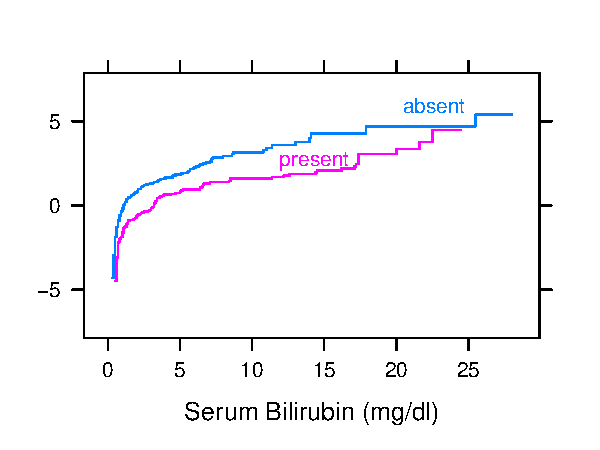
\includegraphics[width=\maxwidth]{nonpar-pbc-1} }

\end{Schunk}

\item The curves are primarily parallel (even at the far left, despite the optical illusion)
\item Nonlinearity is irrelevant
\item Check $t$-test assumptions

\begin{Schunk}
\begin{Sinput}
Ecdf(~ bili, group=spiders, data=pbc, fun=qnorm)
\end{Sinput}


\centerline{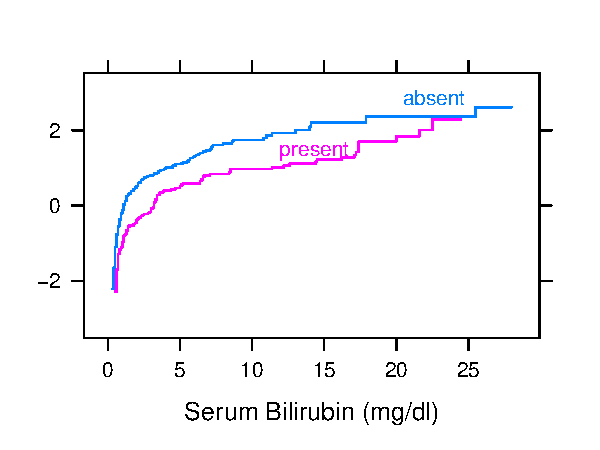
\includegraphics[width=\maxwidth]{nonpar-pbc2-1} }

\end{Schunk}
\item Curves are primarily parallel (variances are equal)
\item \textbf{But} they are not straight lines as required by $t$-test normality assumption
\ei

\section{Power and Sample Size}
\subsection{Normal Approximation}
\bi
\item Common to get power/sample size estimates for the Wilcoxon two-sample comparison using the unpaired $t$-test power formula
\item Are assuming normality and (usually) equal variances
\item To reflect the slight inefficiency of the Wilcoxon two-sample test if normality were to magically hold, multiply the $t$-test sample size by $\frac{\pi}{3} = 1.047$
\item When the response within-group distribution is far from normal this approach is suspect
 \bi
 \item e.g., $Y$ has many ties at one value, has a floor or ceiling effect, is asymmetric, or has heavy tails
 \ei
\item Need a general approach
\ei

\subsection{More on Relative Efficiency}
\bi
\item Relative efficiency of $\frac{3}{\pi}$ for the Wilcoxon 2-sample test can be derived as a correlation coefficient
\item As $n \rightarrow \infty$ it is the squared correlation between the weights Wilcoxon gives to order statistics (sorted data values) and the optimal weights
\item Wilcoxon is a \emph{linear rank statistic} with weights equal to ordinary ranks
\item Optimal linear rank test (normal scores test) for a normal distribution uses the probit link (normal inverse weights), i.e., $\Phi^{-1}(\frac{\textrm{ranks}}{n+1})$
\item Compute correlation of ordinary ranks with normal scores
\begin{Schunk}
\begin{Sinput}
for(n in c(10, 100, 1000, 10000, 100000, 1000000)) {
  ranks  <- 1 : n
  zranks <- qnorm(ranks / (n + 1))
  cat('n:', n, '  r2:', cor(ranks, zranks)^2, '\n')
}
\end{Sinput}
\begin{Soutput}
n: 10   r2: 0.9923288 
n: 100   r2: 0.9688625 
n: 1000   r2: 0.958053 
n: 10000   r2: 0.9554628 
n: 1e+05   r2: 0.955008 
n: 1e+06   r2: 0.9549402 
\end{Soutput}
\begin{Sinput}
cat('3/pi: ', 3 / pi, '\n')
\end{Sinput}
\begin{Soutput}
3/pi:  0.9549297 
\end{Soutput}
\end{Schunk}
\ei

\subsection{Tailoring Power Calculations to the Wilcoxon Test}
\bi
\item Whitehead~\cite{whi93sam} derived simple formulas related to the proportional odds model score test
\item Formulas assume that a frequency-tabulated distribution estimate is available for the combined groups
\item Power is computed as a function of the group 2 : group 1 odds ratio for exceedance probabilities
\item See example below for conversion of ORs to differences in means or medians
 \bi
 \item OR=1 $\rightarrow$ distributions are the same, so differences in means/medians are zero
 \ei
\item See \R\ \co{Hmisc} package \co{popower} and \co{posamsize} functions
\ei

\subsection{Discrete $Y$}
\bi
\item Example: response variable has clumping at zero (with prob.\ 0.3) and is otherwise uniformly distributed over the values 1, 2, 4, 8, 16, 32, 64
 \bi
 \item note: actual data values do not affect power Calculations
 \item don't come into play until translate to means/medians
 \ei
\begin{Schunk}
\begin{Sinput}
p <- c(.3, rep(.1, 7))
popower(p, 1.25, 1000)  # compute power to detect OR=1.25, combined N=1000
\end{Sinput}
\begin{Soutput}
Power: 0.516 
Efficiency of design compared with continuous response: 0.966 
\end{Soutput}
\begin{Sinput}
posamsize(p, 1.25, power=0.9)  # N for power=0.9
\end{Sinput}
\begin{Soutput}
Total sample size: 2621.4 
Efficiency of design compared with continuous response: 0.966 
\end{Soutput}
\end{Schunk}
\item Show how cell probabilities are translated by OR=1.25, and compute the mean and median of Y for a series of ORs for simpler interpretation
\begin{Schunk}
\begin{Sinput}
pomodm(p=p, odds.ratio=1.25)
\end{Sinput}
\begin{Soutput}
[1] 0.25531915 0.09250694 0.09661836 0.10101010 0.10570825 0.11074197 0.11614402
[8] 0.12195122
\end{Soutput}
\begin{Sinput}
x <- c(0, 2 ^ (0:6))
sum(p * x)  # check mean with OR=1
\end{Sinput}
\begin{Soutput}
[1] 12.7
\end{Soutput}
\begin{Sinput}
ors <- c(1, 1.05, 1.1, 1.2, 1.25, 1.5, 2)
w <- matrix(NA, nrow=length(ors), ncol=2, 
            dimnames=list(OR=ors, c('mean', 'median')))
i <- 0
for(or in ors) {
  i <- i + 1
  w[i, ] <- pomodm(x, p, odds.ratio=or)
}
w
\end{Sinput}
\begin{Soutput}
      
OR         mean   median
  1    12.70000 3.000000
  1.05 13.14602 3.364286
  1.1  13.58143 3.709091
  1.2  14.42238 4.350000
  1.25 14.82881 4.650000
  1.5  16.73559 6.000000
  2    20.03640 9.900000
\end{Soutput}
\end{Schunk}
\ei

\subsection{Gaussian $Y$}
\bi
\item Suppose response variable for control group has a normal distribution with mean 100 and SD 10
\item Start by assuming the experimental arm has the same distribution as control except with the mean shifted upwards 3 units
\item This will result in non-proportional odds so the Wilcoxon test is not optimal but will still be 0.95 efficient
\item When the sample size per group is 150, the power of the $t$-test to detect a 3-unit difference in means is:

\begin{Schunk}
\begin{Sinput}
require(pwr)
pwr.t.test(d=3 / 10, n=150, sig.level=0.05, type='two.sample')
\end{Sinput}
\begin{Soutput}

     Two-sample t test power calculation 

              n = 150
              d = 0.3
      sig.level = 0.05
          power = 0.7355674
    alternative = two.sided

NOTE: n is number in *each* group
\end{Soutput}
\end{Schunk}

\item To get the power of the Wilcoxon test when both populations have a normal distribution, we can easily use simulation

\begin{Schunk}
\begin{Sinput}
s <- 1000    # number of simulated trials
pval <- numeric(s)
set.seed(1)  # so can reproduce results
for(i in 1 : s) {
  y1 <- rnorm(150, 100, 10)
  y2 <- rnorm(150, 103, 10)
  w  <- wilcox.test(y1, y2)
  pval[i] <- w$p.value
}
mean(pval < 0.05)   # proportion of simulations with p < 0.05
\end{Sinput}
\begin{Soutput}
[1] 0.713
\end{Soutput}
\begin{Sinput}
# Simulate the power by actually running the prop. odds model 300 times
simRegOrd(300, nsim=400, delta=3, sigma=10)$power    # slower
\end{Sinput}
\begin{Soutput}
[1] 0.71
\end{Soutput}
\end{Schunk}

\item For the Wilcoxon test to be optimal (PO holds) shifting the control distribution by an odds ratio will result in a non-Gaussian distribution for the experimental arm
\item Solve for the odds ratio that shifts the mean from 100 to 103, assume PO and compute the power

\begin{Schunk}
\begin{Sinput}
# Use an arbitrary large sample to mimic population computations
m   <- 200000
y1  <- sort(rnorm(m, 100, 10))
ors <- means <- seq(1, 4, by=.025)
i   <- 0
for(or in ors) {
  i <- i + 1
  means[i] <- pomodm(y1, rep(1/m, m), odds.ratio=or)['mean']
}
plot(ors, means, xlab='Group B:A Odds Ratio',
     ylab='Mean in Population B', type='l')
abline(h=103, col=gray(.85))
needed.or <- approx(means, ors, xout=103)$y
needed.or
\end{Sinput}
\begin{Soutput}
[1] 1.708958
\end{Soutput}
\begin{Sinput}
abline(v=needed.or, col=gray(.85))
# Compute power at that odds ratio assuming no ties in data
popower(rep(1/300, 300), odds.ratio=needed.or, n=300)
\end{Sinput}
\begin{Soutput}
Power: 0.761 
Efficiency of design compared with continuous response: 1 
\end{Soutput}


\centerline{\includegraphics[width=\maxwidth]{nonpar-powerwmean-1} }

\end{Schunk}

\item Check how non-normal the experimental arm responses would be if PO holds and OR=10

\begin{Schunk}
\begin{Sinput}
# First do this theoretically
# Control arm has Gaussian Y with mean 100, SD 10
# Create experimental arm distribution using OR=10
y <- seq(60, 145, length=150)
Fy <- 1 - pnorm(y, mean=100, sd=10)    # P(Y >= y | group A)
Gy <- 1 - plogis(qlogis(Fy) + log(10)) # P(Y >= y | group B)
# Plot new CDF vs. normal approximation agreeing at quartiles
plot(y, Gy, type='l', ylab=expression(P(Y <= y)))
qu <- approx(Gy, y, xout=c(0.25, 0.5, 0.75))$y
qu    # Q1, median, Q2
\end{Sinput}
\begin{Soutput}
[1] 107.3628 113.3506 118.4894
\end{Soutput}
\begin{Sinput}
s <- (qu[3] - qu[1]) / (qnorm(0.75) - qnorm(0.25))
mu <- qu[1] - s * qnorm(0.25)
lines(y, pnorm(y, mean=mu, sd=s), col='blue')   # Gaussian fit
\end{Sinput}


\centerline{\includegraphics[width=\maxwidth]{nonpar-hownn-1} }

\end{Schunk}

\begin{Schunk}
\begin{Sinput}
# Theoretical q-q plot: check linearity of inverse normally transformed
# experimental arm distribution
plot(y, qnorm(Gy), type='l')
abline(lsfit(y, qnorm(Gy)), col='blue')
\end{Sinput}


\centerline{\includegraphics[width=\maxwidth]{nonpar-hownn2-1} }

\end{Schunk}

\begin{Schunk}
\begin{Sinput}
# Compute a new discrete distribution if we convert the control
# distribution using proportional odds
# Done by using a discrete distribution with 200,000 points
p <- pomodm(p=rep(1/m, m), odds.ratio=10)
range(p)  # control arm: all 1/200000
\end{Sinput}
\begin{Soutput}
[1] 5.000023e-07 4.999775e-05
\end{Soutput}
\begin{Sinput}
wtd.mean(y1, p)  # mean shifted by about 12 units
\end{Sinput}
\begin{Soutput}
[1] 112.4126
\end{Soutput}
\begin{Sinput}
# Form new distribution by repeating each observation a number
# of times equal to the ratio of the new probability to the
# minimum of all new probabilities
y2 <- rep(y1, round(p / min(p)))  # 2M obs instead of 200K
mean(y2)
\end{Sinput}
\begin{Soutput}
[1] 112.4714
\end{Soutput}
\begin{Sinput}
quantile(y2, c(.25, .5, .75))
\end{Sinput}
\begin{Soutput}
     25%      50%      75% 
107.4240 113.3446 118.5467 
\end{Soutput}
\begin{Sinput}
# The following plot is similar to the previous one
Ecdf(y2, subtitles=FALSE)
lines(y, pnorm(y, mean=mean(y2), sd=sd(y2)), col='blue')
\end{Sinput}


\centerline{\includegraphics[width=\maxwidth]{nonpar-hownn3-1} }

\end{Schunk}

\item Little non-normality of the 2nd group if the treatment effect operates by multiplying the odds that $Y \geq y$ instead of incrementing the mean
 \bi
 \item relates to similarity of normal and logistic distributions
 \ei
\ei

\subsection{Heavy-tailed $Y$}
\bi
\item Get power to detect a shift in mean of 0.3 units for a heavy-tailed control distribution (t with 4 d.f.) with 150 subjects per group
\item Loss of efficiency of $t$-test
 \bi
 \item mean and SD are no longer optimal data summaries
 \ei
\item Can use above method to compute Wilcoxon power quickly if willing to assume PO
\item Let's not assume PO, and instead use simulation
\item Compare with power of $t$-test
\item Do for both null and non-null cases to verify type I error prob.

\begin{Schunk}
\begin{Sinput}
s <- 1000    # number of simulated trials
pvalt <- pvalw <- numeric(s)
set.seed(1)  # so can reproduce results
for(delta in c(0, 0.3)) {
  for(i in 1 : s) {
    y1 <- rt(150, 4)
    y2 <- rt(150, 4) + delta
    pvalt[i] <- t.test(y1, y2)$p.value
    pvalw[i] <- wilcox.test(y1, y2)$p.value
  }
  cat('Delta:', delta, '\n')
  P <- function(x) round(mean(x), 2)
  cat('Proportion of simulations with W p-value < t p-value:',
      P(pvalw < pvalt), '\n')
  cat('Mean p-value for t:', P(pvalt), '\n')
  cat('Mean p-value for W:', P(pvalw), '\n')
  cat('Power for t:', P(pvalt < 0.05), '\n')
  cat('Power for W:', P(pvalw < 0.05), '\n\n')
}
\end{Sinput}
\begin{Soutput}
Delta: 0 
Proportion of simulations with W p-value < t p-value: 0.51 
Mean p-value for t: 0.5 
Mean p-value for W: 0.49 
Power for t: 0.05 
Power for W: 0.06 

Delta: 0.3 
Proportion of simulations with W p-value < t p-value: 0.73 
Mean p-value for t: 0.17 
Mean p-value for W: 0.12 
Power for t: 0.47 
Power for W: 0.6 
\end{Soutput}
\end{Schunk}

\item \co{Hmisc} \co{simRegOrd} function can also simulate power for an adjusted two-sample comparison if there is one adjustment covariate
\ei

\section{Bayesian Proportional Odds Model}
\bi
\item PO model and other cumulative probability semiparametric ordinal regression models are readily extended to a Bayesian framework
\item Need special care in selecting priors for the intercepts for the continuous $Y$ case
\item Nathan James of Vanderbilt University has an implementation using Stan available at\\
\href{https://github.com/ntjames/bayes\_cpm}{github.com/ntjames/bayes\_cpm}
\item See also the \R\ \co{brms} package: \href{http://bit.ly/brms-ordinal}{bit.ly/brms-ordinal} and this discussion:\\ \href{http://github.com/paul-buerkner/brms/issues/762}{github.com/paul-buerkner/brms/issues/762}
\item Bayesian version of the Wilcoxon test is the posterior probability that $\beta_1 > 0$ in the PO model
\item Advantages of Bayes for PO models:
 \bi
 \item does not need approximations such as large sample normality of $\hat{\beta}$ or $\chi^{2}$ distribution approximation to likelihood ratio test statistic
 \item inference is more interpretable and direct
 \item can bring outside information to the analysis
 \item can incorporate shrinkage/penalization/skepticism and still have exact inference
 \item automatically obtain exact distributions and credible intervals for derived quantities\footnote{One merely takes each posterior sample for the $\alpha$s and $\beta$s and computes the quantity of interest, thereby automatically generating posterior samples for the derived quantity for which quantiles can compute credible intervals, etc.}, e.g.\ mean, quantiles, differences in means and quantiles, differences in exceedance probs, $P(Y=y | X)$
 \item can relax PO assumption without huge instabilities that result from using polytomous logistic models; prior distributions can favor PO while allowing non-PO
 \ei
\ei

%% Usage: knitr slide

\chapter{Correlation}\bmovie{12}\ddisc{12}
\section{Overview}

\begin{center}
\smaller
\begin{tabular}{lllll} \hline
Outcome & Predictor & Normality? & Linearity? & Analysis Method \\ \hline
Interval & Binary & Yes & & 2-sample $t$-test \textbf{or linear regression} \\
Ordinal & Binary & No & & Wilcoxon 2-sample test \\
Categorical & Categorical & & & Pearson $\chi^2$ test \\
Interval & Interval & Yes & Yes & \textbf{Correlation or linear regression} \\ 
Ordinal & Ordinal & No & No & \textbf{Spearman's rank correlation} \\ \hline
\end{tabular}\end{center}

\bi 
\item Examine association between continuous/interval outcome ($y$) and continous/interval predictor ($x$)
\item Scatterplot of $y$ versus $x$
\ei

\section{Pearson's correlation coefficient} \ros{11.1, .7-.8, .12}\katz{5.7.A}
\bi
\item $r = \frac{\Sigma(x_i - \bar{x})(y_i - \bar{y})}{\sqrt{\Sigma(x_i - \bar{x})^2\Sigma(y_i - \bar{y})^2}}$
\item Range: $-1 \leq r \leq 1$
\item Correlation coefficient is a unitless index of strength of association between two variables (+ = positive association, - = negative, 0 = no association)
\item Measures the linear relationship between $X$ and $Y$
\item Can test for significant association by testing whether the population correlation is zero
\beq
t = \frac{r\sqrt{n-2}}{\sqrt{1-r^{2}}}
\eeq
which is identical to the $t$-test used to test whether the population
$r$ is zero; d.f.=$n-2$.
\item Use probability calculator for $t$ distribution to get $P$-value
  (2-tailed if interested in association in either direction)
\item 1-tailed test for a positive correlation between $X$ and $Y$
  tests $H_{0}:$ when $X \uparrow$ does $Y \uparrow$ in the population?
\item Confidence intervals for population $r$ calculated using
  Fisher's $Z$ transformation \ros{11.8}\altman{89-91}
\beq
Z = \frac{1}{2} \textrm{log}_\textrm{e} \left( \frac{1+r}{1-r} \right)
\eeq
 \bi 
 \item For large $n$, Z follows a Normal distribution with standard error $\frac{1}{\sqrt{n-3}}$
 \item To calculate a confidence interval for $r$, first find the confidence interval for $Z$ then transform back to the $r$ scale
 \ei
\begin{eqnarray*}
 Z & = & \frac{1}{2} \textrm{log}_\textrm{e} \left( \frac{1+r}{1-r} \right) \\
 2*Z & = & \textrm{log}_\textrm{e} \left( \frac{1+r}{1-r} \right) \\
 \textrm{exp}(2*Z) & = & \left( \frac{1+r}{1-r} \right) \\
 \textrm{exp}(2*Z) * (1-r) & = & 1 + r \\
 \textrm{exp}(2*Z) - r * \textrm{exp}(2*Z) & = & 1 + r \\
 \textrm{exp}(2*Z) - 1 & = & r * \textrm{exp}(2*Z) + r \\
 \textrm{exp}(2*Z) - 1 & = & r \left(\textrm{exp}(2*Z) + 1\right) \\
 \frac{\textrm{exp}(2*Z) - 1}{\textrm{exp}(2*Z) + 1} & = & r \\
\end{eqnarray*}

 \item Example (Altman 89-90): Pearson's $r$ for a study investigating the association of basal metabolic rate with total energy expenditure was calculated to be $0.7283$ in a study of $13$ women.  Derive a 0.95 confidence interval for $r$.
\beq
 Z = \frac{1}{2} \textrm{log}_\textrm{e} \left( \frac{1+0.7283}{1-0.7283} \right) = 0.9251 \\
\eeq
The lower limit of a 0.95 CI for $Z$ is given by
\beq
  0.9251 - 1.96 * \frac{1}{\sqrt{13-3}} = 0.3053
\eeq
and the upper limit is
\beq
  0.9251 + 1.96 * \frac{1}{\sqrt{13-3}} = 1.545
\eeq
A 0.95 CI for the population correlation coefficient is given by transforming these limits from the $Z$ scale back to the $r$ scale
\beq
  \frac{\textrm{exp}(2*0.3053) - 1}{\textrm{exp}(2*0.3053) + 1} \hspace{.5cm} \textrm{to} \hspace{.5cm}  \frac{\textrm{exp}(2*1.545) - 1}{\textrm{exp}(2*1.545) + 1}
\eeq
Which gives a 0.95 CI from 0.30 to 0.91 for the population correlation
\ei
\begin{Schunk}
\begin{Sinput}
n <- 13
r <- 0.7283
z.transform <- 0.5 * log((1 + r) / (1 - r))
clz <- z.transform + c(-1, 1) * qnorm(0.975) / sqrt(n - 3)
clr <- (exp(2 * clz) - 1) / (exp(2 * clz) + 1)
round(c(z.transform, clz, clr), 4)
\end{Sinput}
\begin{Soutput}
[1] 0.9251 0.3053 1.5449 0.2962 0.9129
\end{Soutput}
\end{Schunk}

\section{Spearman's Rank Correlation}  \ros{11.12}\katz{5.7.B}
\bi
\item Pearson's $r$ assumes linear relationship between $X$ and $Y$
\item Spearman's $\rho$ (sometimes labeled $r_{s}$) assumes monotonic
  relationship between $X$ and $Y$ 
 \bi
 \item when $X \uparrow$, $Y$ always $\uparrow$ or stays flat, or $Y$
   always $\downarrow$ or stays flat
 \item does not assume linearity
 \ei
\item $\rho = r$ once replace column of $X$s by their ranks and column
  of $Y$s by ranks
\item To test $H_{0}:\rho=0$ without assuming linearity or normality,
  being damaged by outliers, or sacrificing much power (even if data are
  normal), use a $t$ statistic:
\beq
t = \frac{\rho\sqrt{n-2}}{\sqrt{1-\rho^{2}}}
\eeq
which is identical to the $t$-test used to test whether the population
$r$ is zero; d.f.=$n-2$.
\item Use probability calculator for $t$ distribution to get $P$-value
  (2-tailed if interested in association in either direction)
\item 1-tailed test for a positive correlation between $X$ and $Y$
  tests $H_{0}:$ when $X \uparrow$ does $Y \uparrow$ in the population?
\ei

\section{Correlation Examples}

\bi 
\item Correlation difficult to judge by eye
\item Example plots on following pages
\ei

\begin{Schunk}
\begin{Sinput}
# Generate 50 data points with Popluation correlations of 0, .2, .4, .6,
# .8, and .9 and plot results
require(ggplot2)
n <- 50
set.seed(123)
x <- rnorm(n, 5, 1)
d <- expand.grid(x=x, R=c(0, .2, .4, .6, .8, .9))
d <- transform(d, y = x + rnorm(nrow(d), 0,
                      ifelse(R == 0, 5, sqrt(R ^ -2 - 1))))
sfun <- function(i) {
  x <- d$x[i]; y <- d$y[i]; R <- d$R[i][1]
  r <- cor(x, y)
  tr <- r * sqrt(n - 2) / sqrt(1 - r^2)
  rho <- cor(rank(x), rank(y))
  trho <- rho * sqrt(n - 2) / sqrt(1 - rho^2)
  label <- paste('True r:', R[1], '  r:', round(r,2), '  t:', round(tr,2),
        '  rho:', round(rho,2), '  t:', round(trho,2), sep='')
  names(label) <- R
  label
  }
stats <- tapply(1 : nrow(d), d$R, sfun)
d$stats <- factor(stats[as.character(d$R)], unique(stats))
   
ggplot(d, aes(x=x, y=y)) + geom_point() + facet_wrap(~ stats) +
  theme(strip.text.x = element_text(size=7))   # Fig. (*\ref{fig:corr-corrplota}*)
\end{Sinput}
\begin{figure}[htbp]

\centerline{\includegraphics[width=\maxwidth]{corr-corrplota-1} }

\caption[Example correlation coefficients]{Samples of size $n=50$ for X and Y are drawn from bivariate normal populations with true correlations ranging from 0.0 to 0.9. Pearson and Spearman sample correlations are shown for samples of size 50.  Besides the population correlation coefficient, each panel is labeled with the estimated Pearson $r$, its $t$ statistic, the estimated Spearman $\rho$, and its $t$ statistic}\label{fig:corr-corrplota}
\end{figure}
\end{Schunk}
\begin{Schunk}
\begin{Sinput}
# Different scenarios that can lead to a correlation of 0.7

set.seed(123)   # Fig. (*\ref{fig:corr-corrplotb}*)
rho <- 0.7; n <- 50
var.eps <- rho^-2 - 1
x <- rnorm(n, 5, 1)
y <- x + rnorm(n, 0, sqrt(var.eps))
cor(x,y)
\end{Sinput}
\begin{Soutput}
[1] 0.6951673
\end{Soutput}
\begin{Sinput}
plot(x,y,xlab='',ylab='')

x <- c(1:20,30)
y <- c(1:20,6.2)
cor(x,y)
\end{Sinput}
\begin{Soutput}
[1] 0.6988119
\end{Soutput}
\begin{Sinput}
plot(x,y,xlab='',ylab='')

set.seed(123)
x <- rnorm(40)
y <- rnorm(40)
x[21] <- y[21] <- 8.5
cor(x,y)
\end{Sinput}
\begin{Soutput}
[1] 0.7014825
\end{Soutput}
\begin{Sinput}
plot(x,y,xlab='',ylab='')

x <- rep(0:19,2)
y <- c(rep(.62,20),rep(2,20)) * x
cor(x,y)
\end{Sinput}
\begin{Soutput}
[1] 0.701783
\end{Soutput}
\begin{Sinput}
plot(x,y,xlab='',ylab='')

x <- -7:12
y <- x^2
cor(x,y)
\end{Sinput}
\begin{Soutput}
[1] 0.6974104
\end{Soutput}
\begin{Sinput}
plot(x,y,xlab='',ylab='')

set.seed(123)
tmp <- 1:20 / 2
x <- c(rnorm(20, tmp, 1), tmp + rnorm(20,14.5,1))
y <- c(rnorm(20, -tmp, 1), -tmp + rnorm(20,14.5,1))
cor(x,y)
\end{Sinput}
\begin{Soutput}
[1] 0.703308
\end{Soutput}
\begin{Sinput}
plot(x,y,xlab='',ylab='')
\end{Sinput}
\begin{figure}[htbp]

\centerline{\includegraphics[width=\maxwidth]{corr-corrplotb-1} }

\caption[Multiple datasets having same Pearson $r$]{Different observed datasets that have the same correlation.  All six plots have a sample Pearson correlation of $0.7$.}\label{fig:corr-corrplotb}
\end{figure}
\end{Schunk}


\clearpage
\section{Correlation and Agreement}

\bi 
 \item Compare two methods of measuring the same underlying value
  \bi 
  \item Lung function measured using a spirometer (expensive, accurate) or peak flow meter (cheap, less accurate)
  \item Two devices (oropharyngeal and conventional) used to mesured
    acidity (pH) in the esophagus as a marker of reflux
  \ei
 \item Typical (incorrect) approach begins with scatterplot of one
   method vs.\ the other with a 1:1 line indicating perfect agreement
 \item See Figure~\ref{fig:descript-pH}
 \item Incorrect approach would report a high correlation ($r = 0.90$) and conclude good agreement
 \item Problems with the correlation approach
  \begin{enumerate}
   \item $r$ measures the degree of linear association between two
     variables, not the agreement.  If, for example, the Sandhill
     consistently gave pH values that were 0.5 unit higher than the
     Restech, we could still have high correlation, but poor agreement
     between the two devices.  We can have high correlation if the two
     devices lie closely to any line, not just a 1:1 line that
     indicates perfect agreement.  
   \item A change in scale does not affect correlation, but does
     influence agreement. For example, if the Sandhill always
     registered 2 times larger than the Restech, we would have perfect
     correlation but the agreement would get progressively worse for
     larger values of pH. 
   \item Correlation depends on the range of the data so that larger
     ranges lead to larger correlations.  This can lead to vary
     strange interpretations 

\begin{table}[!h]
\begin{center}
\begin{tabular}{l|cc}
 & $r$ & $\rho$ \\ \hline
all data & 0.90 & 0.73 \\ 
avg pH $\leq 4$ & 0.51 & 0.58 \\ 
avg pH $> 4$ & 0.74 & 0.65
\end{tabular}
\caption{Pearson ($r$) and Spearman ($\rho$) correlations for Restech and Sandhill pH data.  The correlation calculated using all of the data is larger than the correlation calculated using a retricted range of the data.  However, it would be difficult to claim that the overall agreement is better than both the agreement when pH is less than 4 and when pH is greater than 4.}
\end{center}
\end{table}

\item Tests of significance (testing if $r=0$) are irrelevant to the
  question at hand, but often reported to demonstrate a significant
  association.  The two devices are measuring the same quantity, so it
  would be shocking if we did not observe a highly significant
  $p$-value. A $p < .0001$ is not impressive.  A regression analysis
  with a highly significant slope would be similarly unimpressive. 
\item Data can have high correlation, but poor agreement.  There are
  many examples in the literature, but even in our analysis with $r =
  0.90$, the correlation is high, but we will show that the agreement
  is not as good as the high correlation implies. \
  \end{enumerate}
\ei

See Chapter~\ref{chap:obsvar} for simple approaches to assessing agreement
and analyzing observer variability studies.

\subsection{Bland-Altman Plots} \ems{36.4}

\bi 
  \item See Bland and Altman (1986, Lancet)
  \item Earlier: Tukey mean-difference plot
  \item Create plots of the difference in measurements on the y-axis
    versus the average value of the two devices on the x-axis 
  \item If the two devices agree, the difference should be about zero
  \item The average of the two devices is our best estimate of the
    true, unknown (pH) value that is we are trying to measure 
  \item Measurements will often vary in a systematic way over the
    range of measurement. By plotting the difference versus the
    average, we can visually determine if the difference changes over
    our estimate of the truth. 
  \item Solid line indicated the mean, dashed lines are approximate
    0.95 confidence intervals (assuming Normality) 
\ei

\textbf{But} there is controversy about what should be on the $x$-axis
of the plot.  Krouwer~\cite{kro08why} concluded that:
\bi
\item When the two measures have nearly equal variability, i.e., when
  comparing two ``field measurements'', the Bland-Altman approach is preferred
\item When one measurement is a ``reference standard'' having much less
  variation than the field measurement, the reference standard and not
  the average of the two measurements should be on the $x$-axis
\ei

\begin{Schunk}
\begin{Sinput}
require(Hmisc)
getHdata(esopH)
esopH$diff <- with(esopH, orophar - conv)
ggplot(esopH, aes(x=(conv + orophar)/2, y=diff)) +   # Fig. (*\ref{fig:corr-baplot}*)
  stat_binhex(aes(alpha=..count.., color=Hmisc::cut2(..count.., g=20)),
              bins=80) +
  stat_smooth() +
  geom_hline(yintercept = mean(esopH$diff, na.rm=TRUE) +
   c(-1.96, 0, 1.96) * sd(esopH$diff, na.rm=TRUE),
   linetype=c(2,1,2), color='brown') +
  xlab('Average of Conventional and Oropharyngeal pH') +
  ylab('Oropharyngeal Minus Conventional pH') +
  guides(alpha=FALSE, fill=FALSE, color=guide_legend(title='Frequency'))
\end{Sinput}
\begin{figure}[htbp]

\centerline{\includegraphics[width=\maxwidth]{corr-baplot-1} }

\caption[Bland-Altman plot for 2 pH measurements]{Bland-Altman plot for the oroesophageal and conventional pH measurements, using hexagonal binning because of the large sample size.  The difference in pH mesaurements (oro.\ -conventional) is presented on the $y$-axis and the average of the two devices on the $x$-axis.  We see poor agreement around pH values of 4-5}\label{fig:corr-baplot}
\end{figure}
\end{Schunk}

\bi 
  \item We will also consider differences in the two measurements over the time of day
  \item The added smooth curve is called a locally weighted scatterplot smooth (loess)
\ei

\begin{Schunk}
\begin{Sinput}
getHdata(esopH2)
ggplot(esopH2, aes(x=time, y=diffpH)) +    # Fig. (*\ref{fig:corr-phtimediff}*)
       geom_point(pch='.') + stat_smooth() +
       geom_hline(yintercept = 0, col='gray60') +
       scale_x_continuous(breaks=seq(16, 38, by=4),
                          labels=c("4 PM", "8 PM", "12 AM",
                            "4 AM", "8AM", "12 PM"),
                          limits=c(14, 14+24)) +
       ylab('Average of Oropharyngeal Minus Conventional pH') +
       xlab('Time of Day')
\end{Sinput}
\begin{figure}[htbp]

\centerline{\includegraphics[width=\maxwidth]{corr-phtimediff-1} }

\caption[Difference in pH by time of day]{Difference in pH measurements (oro. - conventional) by time of day along with a loess smoother and pointwise 0.95 confidence bands.  Is the difference modified by a subject being in a supine position rather than being upright?}\label{fig:corr-phtimediff}
\end{figure}
\end{Schunk}

\subsection{Sample Size for $r$}\alabel{sec:corr-n}
\bi
\item Without knowledge of population variances, etc., $r$ can be
  useful for planning studies
\item Choose $n$ so that margin for error (half-width of C.L.) for $r$
  is acceptable
\item Precision of $r$ in estimating $\rho$ is generally worst when $\rho=0$
\item This margin for error as well as that for three other choices of the unknown true $\rho$ are shown in Figure~\ref{fig:corr-moe}.
\begin{Schunk}
\begin{Sinput}
require(Hmisc)
plotCorrPrecision(rho=c(0, .25, .5, .75),
                  n=seq(10, 1000, length=100),
                  ylim=c(0, .4), col=1:4, opts=list(keys='lines'))
abline(h=seq(0, .4, by=0.025),
       v=seq(25, 975, by=25), col=gray(.9))
\end{Sinput}
\begin{figure}[htbp]

\centerline{\includegraphics[width=\maxwidth]{corr-moe-1} }

\caption[Margin of error for estimating correlation coefficient]{Margin for error (length of longer side of asymmetric 0.95 confidence interval) for $r$ in estimating $\rho$, when $\rho=0, 0.25, 0.5, 0.75$.  Calculations are based on Fisher $z$ transformation of $r$.}\label{fig:corr-moe}
\end{figure}
\end{Schunk}
\ei

See also \href{https://stats.stackexchange.com/questions/415131}{stats.stackexchange.com/questions/415131}.

\subsection{Comparing Two $r$'s}
\bi
\item Rarely appropriate
\item Two $r$'s can be the same even though slopes may differ
\item Usually better to compare effects on a real scale (slopes)
\ei

\section{Avoiding Overinterpretation}
\bi
\item Often researchers 
 \bi
 \item compute many correlations then
 \item make a big deal out of the largest observed correlation
 \ei
\item This is \emph{double dipping}: using the same dataset to tell you which features to test, then testing those features
\item This is a ranking and selection problem, and the data seldom contain enough information to be reliable in the choices
\ei

\subsection{Simulate Data}
\bi
\item For our analysis experiments, simulate a sample of size 50 from a 10-variate normal distribution with a known correlation matrix
\item To specify this correlation matrix take the easy way out: compute an observed correlation matrix from a small sample where all correlations in the population are zero
\item The usual sample noise will generate some large observed correlations
\begin{Schunk}
\begin{Sinput}
require(Hmisc)
require(mvtnorm)
\end{Sinput}
\begin{Sinput}
# Get a population correlation matrix by getting sample correlations
# on a random normal sample with N=20 and all true correlations=0
# then pretend these sample correlations were real population values
set.seed(3)
x <- rmvnorm(20, sigma=diag(10))
R <- rcorr(x)$r
# True correlations we will simulate from:
round(R, 2)
\end{Sinput}
\begin{Soutput}
       [,1]  [,2]  [,3]  [,4]  [,5]  [,6]  [,7]  [,8]  [,9] [,10]
 [1,]  1.00  0.01  0.47 -0.09 -0.31 -0.07  0.14  0.05  0.02 -0.49
 [2,]  0.01  1.00  0.48  0.27  0.27  0.14  0.40 -0.17 -0.59  0.60
 [3,]  0.47  0.48  1.00 -0.11  0.26 -0.31  0.45 -0.12 -0.50 -0.06
 [4,] -0.09  0.27 -0.11  1.00  0.42  0.42 -0.07 -0.35  0.16  0.35
 [5,] -0.31  0.27  0.26  0.42  1.00 -0.04  0.03 -0.40 -0.25  0.34
 [6,] -0.07  0.14 -0.31  0.42 -0.04  1.00  0.19 -0.36  0.08  0.40
 [7,]  0.14  0.40  0.45 -0.07  0.03  0.19  1.00 -0.37 -0.65 -0.07
 [8,]  0.05 -0.17 -0.12 -0.35 -0.40 -0.36 -0.37  1.00  0.17 -0.24
 [9,]  0.02 -0.59 -0.50  0.16 -0.25  0.08 -0.65  0.17  1.00 -0.18
[10,] -0.49  0.60 -0.06  0.35  0.34  0.40 -0.07 -0.24 -0.18  1.00
\end{Soutput}
\begin{Sinput}
# Get a huge sample from a multivariate normal distribution to see
# that it mimics the real correlation matrix R
x <- rmvnorm(50000, sigma=R)
table(round(R - rcorr(x)$r, 2))
\end{Sinput}
\begin{Soutput}

-0.01     0  0.01 
   14    76    10 
\end{Soutput}
\begin{Sinput}
# Now sample from the population to get our dataset with N=50
x <- rmvnorm(50, sigma=R)
rorig <- rcorr(x)$r
round(rorig, 2)
\end{Sinput}
\begin{Soutput}
       [,1]  [,2]  [,3]  [,4]  [,5]  [,6]  [,7]  [,8]  [,9] [,10]
 [1,]  1.00 -0.01  0.50  0.11  0.00 -0.16  0.07 -0.04 -0.04 -0.43
 [2,] -0.01  1.00  0.50  0.19  0.43  0.13  0.60 -0.26 -0.76  0.69
 [3,]  0.50  0.50  1.00 -0.15  0.45 -0.41  0.52 -0.18 -0.58 -0.01
 [4,]  0.11  0.19 -0.15  1.00  0.45  0.30 -0.13 -0.35  0.09  0.14
 [5,]  0.00  0.43  0.45  0.45  1.00 -0.12  0.27 -0.53 -0.42  0.20
 [6,] -0.16  0.13 -0.41  0.30 -0.12  1.00  0.06 -0.27  0.00  0.51
 [7,]  0.07  0.60  0.52 -0.13  0.27  0.06  1.00 -0.57 -0.81  0.19
 [8,] -0.04 -0.26 -0.18 -0.35 -0.53 -0.27 -0.57  1.00  0.37 -0.13
 [9,] -0.04 -0.76 -0.58  0.09 -0.42  0.00 -0.81  0.37  1.00 -0.41
[10,] -0.43  0.69 -0.01  0.14  0.20  0.51  0.19 -0.13 -0.41  1.00
\end{Soutput}
\end{Schunk}
\ei

\subsection{Margin of Error for a Single $r$}
\bi
\item First compute the margin of error in estimating a single $r$ from $n=50$
\item This is the spacing between $r$ and it's lower 0.95 CL or the spacing between $r$ and its upper CL whichever is greatest
\item CL based on Fisher's $z$-transformation described earlier
\item Compute this for 4 hypothetical true $r$: 0 0.25 0.5 0.75
\begin{Schunk}
\begin{Sinput}
r <- (0 : 3) / 4
n <- 50
zcrit <- qnorm(0.975)
z <- 0.5 * log( (1 + r) / (1 - r))
lo <- z - zcrit/sqrt(n-3)
hi <- z + zcrit/sqrt(n-3)
rlo <- (exp(2*lo)-1)/(exp(2*lo)+1)
rhi <- (exp(2*hi)-1)/(exp(2*hi)+1)
w <- rbind(r=r, 'Margin of Error'=pmax(rhi - r, r - rlo))
prmatrix(round(w, 2), collab=rep('', 4))
\end{Sinput}
\begin{Soutput}
                                   
r               0.00 0.25 0.50 0.75
Margin of Error 0.28 0.28 0.24 0.15
\end{Soutput}
\end{Schunk}
\item If the true correlation is 0.5, the margin of error in estimating it is $\pm 0.24$ with $n=50$
\ei

\subsection{Bootstrapping the Correlation Selection Process}
\bi
\item Can use the bootstrap to document the difficulty of the task
\item Steps:
 \be 
 \item form a matrix with $N$ rows and $p$ columns where $N$ is the number of observations and $p$ is the number of variables being correlated with each other
 \item draw a sample of size $N$ from this matrix by sampling its rows
 \item compute all the correlation coefficients as was done previously
 \item re-run the same selection process as was done on the original dataset
 \item repeat 1000 times
 \item examine the distribution of the selections over the 1000 repeats
 \ee
\ei

\subsection{Bootstrapping Bias in Largest Observed $r$}
\bi
\item Start with something simpler than ranking all the $r$s in the matrix: estimate the bias in the largest observed $r$
\item Draw a sample with replacement from rows of the data matrix
\item For each of these bootstrap samples find which pair of variables has the highest $r$
\item Track this variable pair and compute $r$ in the original sample
\item Compute the dropoff in $r$ from the bootstrap sample to the original sample
\item This simulates the \emph{process} used to find the largest $r$
\item Example: use data simulated above with 10 standard normal random variables \& known correlation matrix on 50 subjects
\item Sample correlation matrix has $\frac{10 \times 9}{2} = 45$ distinct coefficients
\begin{Schunk}
\begin{Sinput}
# Function to retrieve the upper triangle of a symmetric matrix
# ignoring the diagnonal terms
up <- function(z) z[upper.tri(z)]
rorigu <- up(rorig)
max(rorigu)   # .685 = [2,10] element; 0.604 in population
\end{Sinput}
\begin{Soutput}
[1] 0.6854261
\end{Soutput}
\begin{Sinput}
which.max(rorigu)
\end{Sinput}
\begin{Soutput}
[1] 38
\end{Soutput}
\begin{Sinput}
# is the 38th element in the upper triangle

# Tabulate the difference between sample r estimates and true values
Ru <- up(R)
mean(abs(Ru - rorigu))
\end{Sinput}
\begin{Soutput}
[1] 0.1149512
\end{Soutput}
\begin{Sinput}
table(round(Ru - rorigu, 1))
\end{Sinput}
\begin{Soutput}

-0.3 -0.2 -0.1    0  0.1  0.2 
   2    6    7    7   17    6 
\end{Soutput}
\begin{Sinput}
# Repeat the "finding max r" procedure for 1000 bootstrap samples
# Sample from x 1000 times with replacement, each time computing
# a new correlation matrix
samepair <- dropsum <- 0
for(i in 1 : 1000) {
  b  <- sample(1 : 50, replace=TRUE)
  xb <- x[b, ]   # sample with replacement from rows
  r  <- rcorr(xb)$r
  ru <- up(r)
  wmax <- which.max(ru)
  if(wmax == 38) samepair <- samepair + 1
  # Compute correlation for the bootstrap best pair in the original sample
  origr <- rorigu[wmax]
  # Compute dropoff in best r
  dropoff <- ru[wmax] - origr
  dropsum <- dropsum + dropoff
}
cat('Number of bootstaps selecting the original most correlated pair:',
    samepair, 'out of 1000', '\n')
\end{Sinput}
\begin{Soutput}
Number of bootstaps selecting the original most correlated pair: 642 out of 1000 
\end{Soutput}
\begin{Sinput}
cat('Mean dropoff for max r:', round(dropsum / 1000, 3), '\n')
\end{Sinput}
\begin{Soutput}
Mean dropoff for max r: 0.071 
\end{Soutput}
\end{Schunk}

\item For our dataset with $n=50$ we expect that the maximum observed $r$ out of 45 $r$s is biased high by 0.071
 \bi
 \item Could subtact 0.071 to debias the observed max $r$ although this will worsen its precision
 \ei
\ei

\subsection{Bootstrapping Ranks of All $r$s}
\bi
\item Do a more comprehensive assessment that quantifies the difficulty of the task in ranking all the $r$s
\item Quantity uncertainties in the ranks of the original correlation coefficients
\item Apparent ``winner'' was the one receiving the highest ranking
  $q$ among all $r$s
\item What is the distribution of $q$ over the 1000 bootstrap samples?
\item Can easily compute a 0.95 bootstrap nonparametric percentile confidence interval for the true unknown ranking of that feature combination and for ranking all the examined feature correlations
\item Bootstrap the correlation matrix and re-rank the coefficients
\item For each pair of variables compute the 0.95 confidence interval for the rank of its correlation from among the 45

\begin{Schunk}
\begin{Sinput}
# For each observed correlation compute its rank among 45 distinct pairs
orig.ranks <- rank(up(rorig))
# Sample from x 1000 times with replacement, each time computing
# a new correlation matrix
Rm <- matrix(NA, nrow=1000, ncol=45)
for(i in 1 : 1000) {
  b  <- sample(1 : 50, replace=TRUE)
  xb <- x[b, ]
  r  <- rcorr(xb)$r
  Rm[i, ] <- rank(up(r))
}
# Over bootstrap correlations compute quantiles of ranks
low  <- apply(Rm, 2, quantile, probs=0.025)
high <- apply(Rm, 2, quantile, probs=0.975)
round(cbind('Original Rank'=orig.ranks, Lower=low, Upper=high))
\end{Sinput}
\begin{Soutput}
      Original Rank Lower Upper
 [1,]            22    12    34
 [2,]            40    32    45
 [3,]            41    30    45
 [4,]            28    15    37
 [5,]            31    20    38
 [6,]            15     8    28
 [7,]            24    11    34
 [8,]            37    32    43
 [9,]            38    32    43
[10,]            39    31    44
[11,]            14     8    27
[12,]            29    15    37
[13,]             9     3    15
[14,]            35    22    43
[15,]            18    10    26
[16,]            26    16    34
[17,]            44    38    45
[18,]            43    34    45
[19,]            16     9    27
[20,]            34    25    38
[21,]            25    14    34
[22,]            19    11    32
[23,]            12     7    21
[24,]            13     7    27
[25,]            10     4    20
[26,]             5     3    10
[27,]            11     5    22
[28,]             4     3     8
[29,]            20    10    33
[30,]             2     1     4
[31,]             3     2    11
[32,]            27    16    36
[33,]             7     4    13
[34,]            23    13    32
[35,]             1     1     2
[36,]            36    28    43
[37,]             6     3    15
[38,]            45    40    45
[39,]            21    12    31
[40,]            30    17    37
[41,]            33    21    39
[42,]            42    34    44
[43,]            32    20    38
[44,]            17    11    28
[45,]             8     3    16
\end{Soutput}
\end{Schunk}

\item Highest observed $r$ (rank 45) has 0.95 CI $[40,45]$
\item Data are consistent with it being the $6^\textrm{th}$ highest
\item Smallest observed value (rank 1; most impressive negative
  correlation) has CI $[1, 2]$ for rank; data consistent with that
  pair of variables being the best or $2^\textrm{nd}$
\item The $r$ originally ranked $36^\textrm{th}$ has a 0.95 CI of $[28, 43]$ so the data are consistent with it being in the top 3
\ei

\subsection{Monte Carlo Simulation to Get A Rank Interval}
\bi
\item For comparison with the bootstrap, get the frequency distribution of ranks in repeated studies of the apparently highest $r$ in our $n=50$ study
\item Repeated studies will also have $n=50$ and will be generated from the population correlation matrix
\item Recall that original max $r$ was the $38^\textrm{th}$ element of the strung-out $r$ matrix from our sample
\begin{Schunk}
\begin{Sinput}
ranks <- integer(1000)
for(i in 1 : 1000) {
  xs <- rmvnorm(50, sigma=R)
  rsim <- up(rcorr(xs)$r)
  ranks[i] <- rank(rsim)[38]
}
table(ranks)   # freqs. of ranks of 38th element in new samples
\end{Sinput}
\begin{Soutput}
ranks
 34  35  36  37  38  39  40  41  42  43  44  45 
  2   1   6   8  10  18  25  38  58  88 152 594 
\end{Soutput}
\begin{Sinput}
quantile(ranks, c(0.025, 0.975))
\end{Sinput}
\begin{Soutput}
 2.5% 97.5% 
   38    45 
\end{Soutput}
\end{Schunk}
\item This interval is a bit wider than the bootstrap interval
\item \textbf{Note}: both the bootstrap and the Monte Carlo simulated interval would be \textbf{far wider} had the number of correlation coefficients estimated been much greater than the sample size
\item Example: consider 1000 possible associations with a single $Y$
\item This time the potential predictors $X$ will be independent in the population and they will be conditioned on (held constant over simulations at the original $X$ values)
\item The true importance of the $X$s is $1, 2, \ldots, 10$ for the first 10 and all remaining are irrelevant in the population
\begin{Schunk}
\begin{Sinput}
set.seed(8)
n <- 50
p <- 1000
x <- matrix(rnorm(n * p), ncol=p)
Ey <- x[,1] + 2 * x[,2] + 3 * x[,3] + 4 * x[,4] + 5 * x[,5] + 6 * x[,6] +
      7 * x[,7] + 8 * x[,8] + 9 * x[,9] + 10 * x[,10]
y <- Ey + rnorm(n) * 20
ro <- cor(x, y)
# First 10 correlations and tabulate all others
round(ro[1:10], 2)
\end{Sinput}
\begin{Soutput}
 [1]  0.26 -0.16  0.05  0.29 -0.03  0.04  0.28  0.05  0.28  0.57
\end{Soutput}
\begin{Sinput}
table(round(ro[-(1:10)], 1))
\end{Sinput}
\begin{Soutput}

-0.5 -0.4 -0.3 -0.2 -0.1    0  0.1  0.2  0.3  0.4  0.5 
   1    6   43   97  234  250  210  120   25    3    1 
\end{Soutput}
\begin{Sinput}
# Find which of the 1000 correlation against Y is largest
wmax <- which.max(ro)
wmax     # correct according to population
\end{Sinput}
\begin{Soutput}
[1] 10
\end{Soutput}
\begin{Sinput}
ro[wmax]   # original rank=1000
\end{Sinput}
\begin{Soutput}
[1] 0.5698995
\end{Soutput}
\begin{Sinput}
# Simulate 1000 repeats of sample with new y but keeping x the same
# See how original highest correlating variable ranks among 1000
# correlations in new samples

ranks <- numeric(1000)
for(i in 1 : 1000) {
  ys <- Ey + rnorm(n) * 20
  rs <- cor(x, ys)
  ranks[i] <- rank(rs)[wmax]
}

table(round(ranks, -1))   # round to nearest 10
\end{Sinput}
\begin{Soutput}

 350  400  580  600  610  620  630  660  670  680  690  700  710  720  730  740 
   1    1    1    1    1    2    1    1    4    2    2    2    1    2    1    1 
 760  770  780  790  800  810  820  830  840  850  860  870  880  890  900  910 
   1    1    2    4    6    2    6   11    3    6    6    9   13    8   15   15 
 920  930  940  950  960  970  980  990 1000 
  15   34   39   41   50   66  126  203  294 
\end{Soutput}
\begin{Sinput}
quantile(ranks, c(0.025, 0.975))
\end{Sinput}
\begin{Soutput}
   2.5%   97.5% 
 770.85 1000.00 
\end{Soutput}
\begin{Sinput}
sum(ranks > 998)
\end{Sinput}
\begin{Soutput}
[1] 139
\end{Soutput}
\end{Schunk}

\item The apparent winning variable could fairly easily be the $771^\textrm{st}$ largest instead of the $1000^\textrm{th}$ ranked correlation
\item The winning variable was in the top two in only 139 out of 1000 simulations
\item See Chapter~\ref{chap:hdata} for more ways to quantify limitations of high-dimensional data analysis, including the $p > N$ case
\ei

%% Usage: knitr slide


\def\apacue{1}
\chapter{Introduction to the \R\ \co{rms} Package: The Linear Model}\alabel{chap:rmsintro}
Some of the purposes of the \co{rms} package are to
\bi
\item make everyday statistical modeling easier to do
\item make modern statistical methods easy to incorporate into everyday work
\item make it easy to use the bootstrap to validate models
\item provide ``model presentation graphics''
\ei
  
\section{Formula Language and Fitting Function}%\sound{rrms-1}
\bi
\item Statistical formula in \R:
\begin{Schunk}
\begin{Sinput}
y ~ x1 + x2 + x3
\end{Sinput}
\end{Schunk}
\co{y} \emph{is modeled as} $\alpha + \beta_{1}x_{1} + \beta_{2}x_{2}
+ \beta_{3} x_{3}$.
\item \co{y} is the dependent variable/response/outcome, \co{x}'s are
  predictors (independent variables)
\item The formula is the first argument to a \emph{fitting}
  function (just as it is the first argument to a \co{trellis}
  graphics function)
\item \co{rms} (\emph{regression modeling strategies}) package~\cite{rrms}
  makes many aspects of regression modeling
  and graphical display of model results easier to do
\item \co{rms} does a lot of bookkeeping to
  remember details about the \emph{design matrix} for the model and to
  use these details in making automatic hypothesis tests, estimates,
  and plots.  The design matrix is the matrix of independent variables
  after coding them numerically and adding nonlinear and product terms
  if needed.
\item \co{rms} package fitting function for ordinary least squares
  regression (what is often called the \emph{linear model} or
  \emph{multiple linear regression}): \co{ols}
\item Example:\ipacue
\begin{Schunk}
\begin{Sinput}
f <- ols(y ~ age + sys.bp, data=mydata)
\end{Sinput}
\end{Schunk}
\item \co{age} and \co{sys.bp} are the two predictors (independent
variables) assumed to have linear and additive effects (do not
interact or have synergism)
\item \co{mydata} is an \R\ \emph{data frame} containing at least
  three columns for the model's variables
\item \co{f} (the \emph{fit object}) is an \R\ list object, containing
  coefficients, variances, and many other quantities
\item Below, the fit object will be \co{f} throughout.  In practice,
  use any legal \R\  name, e.g. \co{fit.full.model}
\ei

\section{Operating on the Fit Object}%\sound{rrms-2}
\bi
\item Regression coefficient estimates may be obtained by any of the
  methods listed below
\begin{Schunk}
\begin{Sinput}
f$coefficients
f$coef          # abbreviation
coef(f)         # use the coef extractor function
coef(f)[1]      # get intercept
f$coef[2]       # get 2nd coefficient (1st slope)
f$coef['age']   # get coefficient of age
coef(f)['age']  # ditto
\end{Sinput}
\end{Schunk}
\item But often we use \emph{methods} which do something more
  interesting with the model fit.
 \begin{description}
 \item[\co{print(f)}]: print coefficients, standard errors, $t$-test,
   other statistics; can also just type \co{f} to print
 \item[\co{fitted(f)}]: compute $\hat{y}$
 \item[\co{predict(f, newdata)}]: get predicted values, for subjects
   described in data frame \co{newdata}\footnote{You can get
     confidence limits for predicted means or predicted individual
     responses using the \co{conf.int} and \co{conf.type} arguments to
     \co{predict}.  \co{predict(f)} without the \co{newdata} argument
     yields the same result as \co{fitted(f)}.}
 \item[\co{r <- resid(f)}]: compute the vector of $n$ residuals
   (here, store it in \co{r})
 \item[\co{formula(f)}]: print the regression formula fitted
 \item[\co{anova(f)}]: print ANOVA table for all total and partial
   effects
 \item[\co{summary(f)}]: print estimates partial effects using
   meaningful changes in predictors
 \item[\co{Predict(f)}]: compute predicted values varying a few
   predictors at a time (convenient for plotting)
 \item[\co{ggplot(p)}]: plot partial effects, with predictor ranging
   over the $x$-axis, where \co{p} is the result of \co{Predict}
 \item[\co{g <- Function(f)}]: create an \R\ function that
   evaluates the analytic form of the fitted function
 \item[\co{nomogram(f)}]: draw a nomogram of the model
 \end{description}
\ei

\section{The \co{rms} \co{datadist} Function}%sound{rrms-3}%
\ipacue
To use \co{Predict, summary}, or \co{nomogram} in the \co{rms}
  package, you need to let \co{rms} first compute summaries of the
  distributional characteristics of the predictors:
\begin{Schunk}
\begin{Sinput}
dd <- datadist(x1,x2,x3,...)   # generic form
dd <- datadist(age, sys.bp, sex)
dd <- datadist(mydataframe)    # for a whole data frame
options(datadist='dd')         # let rms know where to find
\end{Sinput}
\end{Schunk}
Note that the name \co{dd} can be any name you choose as long as you
use the same name in quotes to \co{options} that you specify
(unquoted) to the left of <- \co{datadist(...)}.  It is best to
invoke \co{datadist} early in your program before fitting any
models.  That way the \co{datadist} information is stored in the fit
  object so the model is self-contained.  That allows you to make
  plots in later sessions without worrying about \co{datadist}.  \\
\co{datadist} must be re-run if you add a new predictor or recode an
old one.  You can update it using for example
\begin{Schunk}
\begin{Sinput}
dd <- datadist(dd, cholesterol, height)
# Adds or replaces cholesterol, height summary stats in dd
\end{Sinput}
\end{Schunk}

\section{Short Example}\alabel{sec:rmsintro-leadcontinuous}\ipacue\sound{rrms-4}\bmovie{15}\ddisc{15}
Consider the lead exposure dataset from B.\ Rosner \emph{Fundamentals
  of Biostatistics} and originally from Landrigan PJ~\emph{et al}, Lancet
1:708-715, March 29, 1975.  The study was of psychological and
neurologic well-being of children who lived near a lead smelting
plant.  The primary outcome measures are the Wechsler full-scale IQ
score (\co{iqf}) and the finger-wrist tapping score \co{maxfwt}.  The
dataset is available at \url{hbiostat.org/data}
and can be automatically downloaded and \co{load()}'d into \R\ using
the \co{Hmisc} package \co{getHdata} function.  For now we just
analyze lead exposure levels in 1972 and 1973, age, and
\co{maxfwt}\footnote{\co{maxfwt} might be better analyzed as an
  ordinal variable but as will be seen by residual plots it is also
  reasonably considered to be continuous and to satisfy ordinary
  regression assumptions.}.

\textbf{Note}: To easily run all the following commands, open \ipacue
\url{http://fharrell.com/code/bbr.zip}
and then open the file \co{8-rmsintro.r} contained in the \co{.zip}
file using \co{RStudio}.  Commands listed in previous sections were
not actually executed so they are marked with the \R\ comment symbol
(\#) and can be ignored.

\begin{Schunk}
\begin{Sinput}
# For an Rmarkdown version of similar analyses see
# https://github.com/harrelfe/rscripts/raw/master/lead-ols.md
require(rms)    # also loads the Hmisc package
\end{Sinput}
\begin{Sinput}
getHdata(lead)
# Subset variables just so contents() and describe() output is short
# Override units of measurement to make them legal R expressions
lead <- upData(lead,
               keep=c('ld72', 'ld73', 'age', 'maxfwt'),
               labels=c(age='Age'),
               units=c(age='years', ld72='mg/100*ml', ld73='mg/100*ml'))
\end{Sinput}
\begin{Soutput}
Input object size:	 53928 bytes;	 39 variables	 124 observations
Kept variables	ld72,ld73,age,maxfwt
New object size:	14096 bytes;	4 variables	124 observations
\end{Soutput}
\begin{Sinput}
contents(lead)
\end{Sinput}
\begin{Soutput}

Data frame:lead	124 observations and 4 variables    Maximum # NAs:25


                                        Labels     Units Storage NAs
age                                        Age     years  double   0
ld72                   Blood Lead Levels, 1972 mg/100*ml integer   0
ld73                   Blood Lead Levels, 1973 mg/100*ml integer   0
maxfwt Maximum mean finger-wrist tapping score           integer  25
\end{Soutput}
\begin{Sinput}
describe(lead)   # (*\ipacue*)
\end{Sinput}
\begin{Soutput}
lead 

 4  Variables      124  Observations
--------------------------------------------------------------------------------
age : Age [years] 
       n  missing distinct     Info     Mean      Gmd      .05      .10 
     124        0       73        1    8.935    4.074    3.929    4.333 
     .25      .50      .75      .90      .95 
   6.167    8.375   12.021   14.000   15.000 

lowest :  3.750000  3.833333  3.916667  4.000000  4.166667
highest: 14.250000 15.000000 15.250000 15.416667 15.916667
--------------------------------------------------------------------------------
ld72 : Blood Lead Levels, 1972 [mg/100*ml] 
       n  missing distinct     Info     Mean      Gmd      .05      .10 
     124        0       47    0.999    36.16    17.23    18.00    21.00 
     .25      .50      .75      .90      .95 
   27.00    34.00    43.00    57.00    61.85 

lowest :  1  2 10 14 18, highest: 62 64 66 68 99
--------------------------------------------------------------------------------
ld73 : Blood Lead Levels, 1973 [mg/100*ml] 
       n  missing distinct     Info     Mean      Gmd      .05      .10 
     124        0       37    0.998    31.71    11.06    18.15    21.00 
     .25      .50      .75      .90      .95 
   24.00    30.50    37.00    47.00    50.85 

lowest : 15 16 18 19 20, highest: 52 53 54 57 58
--------------------------------------------------------------------------------
maxfwt : Maximum mean finger-wrist tapping score 
       n  missing distinct     Info     Mean      Gmd      .05      .10 
      99       25       40    0.998    51.96     13.8     33.2     38.0 
     .25      .50      .75      .90      .95 
    46.0     52.0     59.0     65.0     72.2 

lowest : 13 14 23 26 34, highest: 74 76 79 83 84
--------------------------------------------------------------------------------
\end{Soutput}
\begin{Sinput}
dd <- datadist(lead); options(datadist='dd')
dd    # show what datadist computed (*\ipacue*)
\end{Sinput}
\begin{Soutput}
                      age  ld72  ld73 maxfwt
Low:effect       6.166667 27.00 24.00   46.0
Adjust to        8.375000 34.00 30.50   52.0
High:effect     12.020833 43.00 37.00   59.0
Low:prediction   3.929167 18.00 18.15   33.2
High:prediction 15.000000 61.85 50.85   72.2
Low              3.750000  1.00 15.00   13.0
High            15.916667 99.00 58.00   84.0
\end{Soutput}
\begin{Sinput}
# Fit an ordinary linear regression model with 3 predictors assumed linear
f <- ols(maxfwt ~ age + ld72 + ld73, data=lead)
f         # same as print(f)  (*\ipacue*)
\end{Sinput}
\begin{Soutput}
Frequencies of Missing Values Due to Each Variable
maxfwt    age   ld72   ld73 
    25      0      0      0 

Linear Regression Model
 
 ols(formula = maxfwt ~ age + ld72 + ld73, data = lead)
 
 
                 Model Likelihood    Discrimination    
                       Ratio Test           Indexes    
 Obs      99    LR chi2     62.25    R2       0.467    
 sigma9.5221    d.f.            3    R2 adj   0.450    
 d.f.     95    Pr(> chi2) 0.0000    g       10.104    
 
 Residuals
 
      Min       1Q   Median       3Q      Max 
 -33.9958  -4.9214   0.7596   5.1106  33.2590 
 
 
           Coef    S.E.   t     Pr(>|t|)
 Intercept 34.1059 4.8438  7.04 <0.0001 
 age        2.6078 0.3231  8.07 <0.0001 
 ld72      -0.0246 0.0782 -0.31 0.7538  
 ld73      -0.2390 0.1325 -1.80 0.0744  
 
\end{Soutput}
\begin{Sinput}
coef(f)   # retrieve coefficients
\end{Sinput}
\begin{Soutput}
 Intercept        age       ld72       ld73 
34.1058551  2.6078450 -0.0245978 -0.2389695 
\end{Soutput}
\begin{Sinput}
specs(f, long=TRUE)   # show how parameters are assigned to predictors, (*\ipacue*)
\end{Sinput}
\begin{Soutput}
ols(formula = maxfwt ~ age + ld72 + ld73, data = lead)

     Units     Label                   Assumption Parameters d.f.
age  years     Age                     asis                  1   
ld72 mg/100*ml Blood Lead Levels, 1972 asis                  1   
ld73 mg/100*ml Blood Lead Levels, 1973 asis                  1   

                      age  ld72  ld73
Low:effect       6.166667 27.00 24.00
Adjust to        8.375000 34.00 30.50
High:effect     12.020833 43.00 37.00
Low:prediction   3.929167 18.00 18.15
High:prediction 15.000000 61.85 50.85
Low              3.750000  1.00 15.00
High            15.916667 99.00 58.00
\end{Soutput}
\begin{Sinput}
                      # and predictor distribution summaries driving plots
g <- Function(f)  # create an R function that represents the fitted model (*\ipacue*)
# Note that the default values for g's arguments are medians
g
\end{Sinput}
\begin{Soutput}
function (age = 8.375, ld72 = 34, ld73 = 30.5) 
{
    34.105855 + 2.607845 * age - 0.024597799 * ld72 - 0.23896951 * 
        ld73
}
<environment: 0x55daa37b6f40>
\end{Soutput}
\begin{Sinput}
# Estimate mean maxfwt at age 10, .1 quantiles of ld72, ld73 and .9 quantile of ld73
# keeping ld72 at .1 quantile
g(age=10, ld72=21, ld73=c(21, 47))  # more exposure in 1973 decreased y by 6
\end{Sinput}
\begin{Soutput}
[1] 54.64939 48.43618
\end{Soutput}
\begin{Sinput}
# Get the same estimates another way but also get std. errors (*\ipacue*)
predict(f, data.frame(age=10, ld72=21, ld73=c(21, 47)), se.fit=TRUE)
\end{Sinput}
\begin{Soutput}
$linear.predictors
       1        2 
54.64939 48.43618 

$se.fit
       1        2 
1.391858 3.140361 
\end{Soutput}
\end{Schunk}

\section{Operating on Residuals}\sound{rrms-5}
Residuals may be summarized and plotted just like any raw data
variable.
\bi
\item To plot residuals vs.\ each predictor, and to make a q-q plot to check normality of residuals, use these examples:
\begin{Schunk}
\begin{Sinput}
r <- resid(f)
par(mfrow=c(2,2))   # 2x2 matrix of plots
plot(fitted(f), r); abline(h=0)  # yhat vs. r
with(lead, plot(age,  r));    abline(h=0)
with(lead, plot(ld73, r));    abline(h=0)
qqnorm(r)           # linearity indicates normality
qqline(as.numeric(r))
\end{Sinput}


\centerline{\includegraphics[width=\maxwidth]{rmsintro-unnamed-chunk-7-1} }

\end{Schunk}
\ei

\section{Plotting Partial Effects}\sound{rrms-6}
\bi
\item \co{Predict} and \co{ggplot} makes one plot for each predictor
\item Predictor is on $x$-axis, $\hat{y}$ on the $y$-axis
\item Predictors not shown in plot are set to constants
 \bi
 \item median for continuous predictors
 \item mode for categorical ones
 \ei
\item For categorical predictor, estimates are shown only at data
  values
\item 0.95 pointwise confidence limits for $\hat{E}(y|x)$ are shown
  (add \co{conf.int=FALSE} to \co{Predict()} to suppress CLs)
\item Example: \ipacue
\begin{Schunk}
\begin{Sinput}
ggplot(Predict(f))
\end{Sinput}


\centerline{\includegraphics[width=\maxwidth]{rmsintro-unnamed-chunk-8-1} }

\end{Schunk}
\item To take control of which predictors are plotted, or to specify
  customized options: \ipacue
\begin{Schunk}
\begin{Sinput}
ggplot(Predict(f, age))   # plot age effect, using default range,
                          # 10th smallest to 10th largest age
\end{Sinput}


\centerline{\includegraphics[width=\maxwidth]{rmsintro-unnamed-chunk-9-1} }

\end{Schunk}
\begin{Schunk}
\begin{Sinput}
ggplot(Predict(f, age=3:15))  # plot age=3,4,...,15 (*\ipacue*)
\end{Sinput}


\centerline{\includegraphics[width=\maxwidth]{rmsintro-unnamed-chunk-10-1} }

\end{Schunk}
\begin{Schunk}
\begin{Sinput}
ggplot(Predict(f, age=seq(3,16,length=150)))   # plot age=3-16, 150 points (*\ipacue*)
\end{Sinput}


\centerline{\includegraphics[width=\maxwidth]{rmsintro-unnamed-chunk-11-1} }

\end{Schunk}
\item To get confidence limits for $\hat{y}$: \ipacue
\begin{Schunk}
\begin{Sinput}
ggplot(Predict(f, age, conf.type='individual'))
\end{Sinput}


\centerline{\includegraphics[width=\maxwidth]{rmsintro-unnamed-chunk-12-1} }

\end{Schunk}
\item To show both types of 0.99 confidence limits on one plot: \ipacue
\begin{Schunk}
\begin{Sinput}
p1 <- Predict(f, age, conf.int=0.99, conf.type='individual')
p2 <- Predict(f, age, conf.int=0.99, conf.type='mean')
p <- rbind(Individual=p1, Mean=p2)
ggplot(p)
\end{Sinput}


\centerline{\includegraphics[width=\maxwidth]{rmsintro-unnamed-chunk-13-1} }

\end{Schunk}
\item Non-plotted variables are set to reference values (median and
  mode by default)
\item To control the settings of non-plotted values use e.g. \ipacue
\begin{Schunk}
\begin{Sinput}
ggplot(Predict(f, ld73, age=3))
\end{Sinput}


\centerline{\includegraphics[width=\maxwidth]{rmsintro-unnamed-chunk-14-1} }

\end{Schunk}
\item To make separate lines for two ages: \ipacue
\begin{Schunk}
\begin{Sinput}
ggplot(Predict(f, ld73, age=c(3,9)))  # add ,conf.int=FALSE to suppress conf. bands
\end{Sinput}


\centerline{\includegraphics[width=\maxwidth]{rmsintro-unnamed-chunk-15-1} }

\end{Schunk}
\item To plot a 3-d surface for two continuous predictors against
  $\hat{y}$; color coding for predicted mean \co{maxfwt} \ipacue
\begin{Schunk}
\begin{Sinput}
bplot(Predict(f, ld72, ld73))
\end{Sinput}


\centerline{\includegraphics[width=\maxwidth]{rmsintro-unnamed-chunk-16-1} }

\end{Schunk}
\ei

\section{Nomograms: Overall Depiction of Fitted Models} \sound{rrms-7}\ipacue
\begin{Schunk}
\begin{Sinput}
plot(nomogram(f))
\end{Sinput}


\centerline{\includegraphics[width=\maxwidth]{rmsintro-unnamed-chunk-17-1} }

\end{Schunk}
See \href{http://stats.stackexchange.com/questions/155430/clarifications-regarding-reading-a-nomogram}{this}
for excellent examples showing how to read such nomograms.

\subsection{Point Estimates for Partial Effects} \sound{rrms-8}\ipacue
The \co{summary} function can compute point estimates and confidence
intervals for effects of individual predictors, holding other
predictors to selected constants.  The constants you hold other
predictors to will only matter when the other predictors interact with
the predictor whose effects are being displayed.

How predictors are changed depend on the type of predictor:
\bi
\item Categorical predictors: differences against the reference (most
  frequent) cell by default
\item Continuous predictors: inter-quartile-range effects by default
\ei
The estimated effects depend on the type of model:
\bi
\item \co{ols}: differences in means
\item logistic models: odds ratios and their logs
\item Cox models: hazard ratios and their logs
\item quantile regression: differences in quantiles
\ei

\begin{Schunk}
\begin{Sinput}
summary(f)         # inter-quartile-range effects (*\ipacue*)
\end{Sinput}
\begin{Soutput}
             Effects              Response : maxfwt 

 Factor Low     High   Diff.   Effect   S.E.   Lower 0.95 Upper 0.95
 age     6.1667 12.021  5.8542 15.26700 1.8914 11.5120    19.02200  
 ld72   27.0000 43.000 16.0000 -0.39356 1.2511 -2.8773     2.09010  
 ld73   24.0000 37.000 13.0000 -3.10660 1.7222 -6.5255     0.31234  
\end{Soutput}
\begin{Sinput}
summary(f, age=5)  # adjust age to 5 when examining ld72,ld73
\end{Sinput}
\begin{Soutput}
             Effects              Response : maxfwt 

 Factor Low     High   Diff.   Effect   S.E.   Lower 0.95 Upper 0.95
 age     6.1667 12.021  5.8542 15.26700 1.8914 11.5120    19.02200  
 ld72   27.0000 43.000 16.0000 -0.39356 1.2511 -2.8773     2.09010  
 ld73   24.0000 37.000 13.0000 -3.10660 1.7222 -6.5255     0.31234  
\end{Soutput}
\begin{Sinput}
                   # (no effect since no interactions in model)
summary(f, ld73=c(20, 40))  # effect of changing ld73 from 20 to 40
\end{Sinput}
\begin{Soutput}
             Effects              Response : maxfwt 

 Factor Low     High   Diff.   Effect   S.E.   Lower 0.95 Upper 0.95
 age     6.1667 12.021  5.8542 15.26700 1.8914  11.5120   19.02200  
 ld72   27.0000 43.000 16.0000 -0.39356 1.2511  -2.8773    2.09010  
 ld73   20.0000 40.000 20.0000 -4.77940 2.6495 -10.0390    0.48052  
\end{Soutput}
\end{Schunk}

When a predictor has a linear effect, its slope is the one-unit change
in $Y$ when the predictor increases by one unit.  So the following
trick can be used to get a confidence interval for a slope: use
\co{summary} to get the confidence interval for the one-unit change:

\begin{Schunk}
\begin{Sinput}
summary(f, age=5:6)    # starting age irrelevant since age is linear (*\ipacue*)
\end{Sinput}
\begin{Soutput}
             Effects              Response : maxfwt 

 Factor Low High Diff. Effect   S.E.    Lower 0.95 Upper 0.95
 age     5   6    1     2.60780 0.32308  1.9664    3.24920   
 ld72   27  43   16    -0.39356 1.25110 -2.8773    2.09010   
 ld73   24  37   13    -3.10660 1.72220 -6.5255    0.31234   
\end{Soutput}
\end{Schunk}

There is a \co{plot} method for \co{summary} results.  By default it
shows 0.9, 0.95, and 0.99 confidence limits. \ipacue
\begin{Schunk}
\begin{Sinput}
plot(summary(f))
\end{Sinput}


\centerline{\includegraphics[width=\maxwidth]{rmsintro-unnamed-chunk-20-1} }

\end{Schunk}

\section{Getting Predicted Values}\sound{rrms-9}
\bi
\item Using \co{predict}
\begin{Schunk}
\begin{Sinput}
predict(f, data.frame(age=3, ld72=21, ld73=21))
\end{Sinput}
\begin{Soutput}
       1 
36.39448 
\end{Soutput}
\begin{Sinput}
# must specify all variables in the model

predict(f, data.frame(age=c(3, 10), ld72=21, ld73=c(21, 47)))
\end{Sinput}
\begin{Soutput}
       1        2 
36.39448 48.43618 
\end{Soutput}
\begin{Sinput}
# predictions for (3,21,21) and (10,21,47)

newdat <- expand.grid(age=c(4, 8), ld72=c(21, 47), ld73=c(21, 47))
newdat
\end{Sinput}
\begin{Soutput}
  age ld72 ld73
1   4   21   21
2   8   21   21
3   4   47   21
4   8   47   21
5   4   21   47
6   8   21   47
7   4   47   47
8   8   47   47
\end{Soutput}
\begin{Sinput}
predict(f, newdat)     # 8 predictions
\end{Sinput}
\begin{Soutput}
       1        2        3        4        5        6        7        8 
39.00232 49.43370 38.36278 48.79416 32.78911 43.22049 32.14957 42.58095 
\end{Soutput}
\begin{Sinput}
predict(f, newdat, conf.int=0.95)  # also get CLs for mean (*\ipacue*)
\end{Sinput}
\begin{Soutput}
$linear.predictors
       1        2        3        4        5        6        7        8 
39.00232 49.43370 38.36278 48.79416 32.78911 43.22049 32.14957 42.58095 

$lower
       1        2        3        4        5        6        7        8 
33.97441 46.23595 32.15468 43.94736 25.68920 36.94167 27.17060 38.86475 

$upper
       1        2        3        4        5        6        7        8 
44.03023 52.63145 44.57088 53.64095 39.88902 49.49932 37.12854 46.29716 
\end{Soutput}
\begin{Sinput}
predict(f, newdat, conf.int=0.95, conf.type='individual')  # CLs for indiv.
\end{Sinput}
\begin{Soutput}
$linear.predictors
       1        2        3        4        5        6        7        8 
39.00232 49.43370 38.36278 48.79416 32.78911 43.22049 32.14957 42.58095 

$lower
       1        2        3        4        5        6        7        8 
19.44127 30.26132 18.46566 29.27888 12.59596 23.30120 12.60105 23.31531 

$upper
       1        2        3        4        5        6        7        8 
58.56337 68.60609 58.25989 68.30944 52.98227 63.13979 51.69810 61.84659 
\end{Soutput}
\end{Schunk}
See also \co{gendata}.
\item The brute-force way
\begin{Schunk}
\begin{Sinput}
# Model is b1 + b2*age + b3*ld72 + b4*ld73
b <- coef(f)
# For 3 year old with both lead exposures 21
b[1] + b[2]*3 + b[3]*21 + b[4]*21
\end{Sinput}
\begin{Soutput}
Intercept 
 36.39448 
\end{Soutput}
\end{Schunk}
\item Using \co{Function} function \ipacue
\begin{Schunk}
\begin{Sinput}
g <- Function(f)
g(age=c(3, 8), ld72=21, ld73=21)       # 2 predictions
\end{Sinput}
\begin{Soutput}
[1] 36.39448 49.43370
\end{Soutput}
\begin{Sinput}
g(age=3)              # 3 year old at median ld72, ld73
\end{Sinput}
\begin{Soutput}
[1] 33.80449
\end{Soutput}
\end{Schunk}
\ei

\section{ANOVA}\sound{rrms-10}
\bi
\item Use \co{anova(fitobject)} to get all total effects and
  individual partial effects
\item Use \co{anova(f,age,sex)} to get combined partial effects of
  \co{age} and \co{sex}, for example
\item Store result of \co{anova} in an object in you want to print it
  various ways, or to plot it:
\begin{Schunk}
\begin{Sinput}
an <- anova(f)
an                     # same as print(an)
\end{Sinput}
\begin{Soutput}
                Analysis of Variance          Response: maxfwt 

 Factor     d.f. Partial SS  MS          F     P     
 age         1   5907.535742 5907.535742 65.15 <.0001
 ld72        1      8.972994    8.972994  0.10 0.7538
 ld73        1    295.044370  295.044370  3.25 0.0744
 REGRESSION  3   7540.087710 2513.362570 27.72 <.0001
 ERROR      95   8613.750674   90.671060             
\end{Soutput}
\begin{Sinput}
print(an, 'names')     # print names of variables being tested
\end{Sinput}
\begin{Soutput}
                Analysis of Variance          Response: maxfwt 

 Factor     d.f. Partial SS  MS          F     P      Tested       
 age         1   5907.535742 5907.535742 65.15 <.0001 age          
 ld72        1      8.972994    8.972994  0.10 0.7538 ld72         
 ld73        1    295.044370  295.044370  3.25 0.0744 ld73         
 REGRESSION  3   7540.087710 2513.362570 27.72 <.0001 age,ld72,ld73
 ERROR      95   8613.750674   90.671060                           
\end{Soutput}
\begin{Sinput}
print(an, 'subscripts')# print subscripts in coef(f) (ignoring (*\ipacue*)
\end{Sinput}
\begin{Soutput}
                Analysis of Variance          Response: maxfwt 

 Factor     d.f. Partial SS  MS          F     P      Tested
 age         1   5907.535742 5907.535742 65.15 <.0001 1     
 ld72        1      8.972994    8.972994  0.10 0.7538 2     
 ld73        1    295.044370  295.044370  3.25 0.0744 3     
 REGRESSION  3   7540.087710 2513.362570 27.72 <.0001 1-3   
 ERROR      95   8613.750674   90.671060                    

Subscripts correspond to:
[1] age  ld72 ld73
\end{Soutput}
\begin{Sinput}
                       # the intercept) being tested
print(an, 'dots')      # a dot in each position being tested
\end{Sinput}
\begin{Soutput}
                Analysis of Variance          Response: maxfwt 

 Factor     d.f. Partial SS  MS          F     P      Tested
 age         1   5907.535742 5907.535742 65.15 <.0001 .     
 ld72        1      8.972994    8.972994  0.10 0.7538  .    
 ld73        1    295.044370  295.044370  3.25 0.0744   .   
 REGRESSION  3   7540.087710 2513.362570 27.72 <.0001 ...   
 ERROR      95   8613.750674   90.671060                    

Subscripts correspond to:
[1] age  ld72 ld73
\end{Soutput}
\begin{Sinput}
anova(f, ld72, ld73)   # combine effects into a 2 d.f. test (*\ipacue*)
\end{Sinput}
\begin{Soutput}
                Analysis of Variance          Response: maxfwt 

 Factor     d.f. Partial SS  MS         F    P     
 ld72        1      8.972994   8.972994 0.10 0.7538
 ld73        1    295.044370 295.044370 3.25 0.0744
 REGRESSION  2    747.283558 373.641779 4.12 0.0192
 ERROR      95   8613.750674  90.671060            
\end{Soutput}
\end{Schunk}
\ei
\def\apacue{0}

%% Usage: knitr slide


\chapter{Simple and Multiple Regression Models}
{\larger\textbf{Background}}\sound{reg-1}

Regression models are used for
\bi
\item hypothesis testing
\item estimation
\item prediction
\item increasing power and precision for assessing the effect of one
  variable by adjusting for other variables that partially explain the outcome
  variable $Y$
\item confounder adjustment---getting adjusted estimates of effects
\item checking that existing summary scores (e.g., BMI) adequately
  summarize their component variables
  \bi
  \item fit a model with log height and log weight and see if ratio of
    coefficients is -2
  \ei
\item determining whether change, average, or most recent measurement
  should be emphasized
  \bi
  \item fit a model containing body weight measured 1y ago and at time
    of treatment initiation
  \item if simple change score is an adequate summary of the two
    weights, the ratio of their coefficients will be about -1
  \item if most recent weight is all-important, coefficient for weight
    1y ago will be very small
  \ei
\item developing new summary scores guided by predicting outcomes
\ei

{\larger\textbf{Example}}
\bi
\item Observational study of patients receiving treatments A and B
\item Females are more likely to receive treatment B $\rightarrow$
  need to adjust for sex
\item Regression approach: fit a model with covariates (predictors)
  treatment and sex; treatment effect is adjusted for sex
\item Stratification approach: for males estimate the B-A difference
  and do likewise for females\\Average of the two differences is
  adjusted for sex
\ei

Now instead of sex being the relevant adjustment variable suppose it
is age, and older patients tend to get treatment B
\bi
\item Regression approach: fit a model with treatment and
  age\\Treatment effect attempts to estimate the B-A difference at any
  chosen (fixed; conditioned on) age
\item Stratification approach:
  \bi
  \item divide age into quintiles
  \item within each quintile compute the B-A difference
  \item average these differences to get an almost age-adjusted
    treatment effect
  \item problem with residual heterogeneity of age within quintiles,
    especially at outer quintiles which are wider
  \ei
\item Matching approach:
  \bi
  \item for each patient on A find a patient on B within 2y of same age
  \item if no match exists discard the A patient
  \item don't use the same B patient again
  \item discard B patients who were not needed to match an A
  \item do a matched pairs analysis, e.g. paired $t$-test
  \item sample size is reduced $\rightarrow \downarrow$ power
  \ei
\ei

\section{Stratification vs.\ Matching vs.\ Regression}%
\movie{https://youtu.be/IiJ6pMs2BiA}\disc{reg-alt}
\bi
\item Some ways to hold one variable $x_1$ constant when estimating the
  effect of another variable $x_2$ (\emph{covariable adjustment}):
  \bi
  \item experimental manipulation of $x_1$
  \item stratify the data on $x_1$ and for each stratum analyze the
    relationship between $x_2$ and $Y$
  \item form matched sets of observations on the basis of $x_1$ and
    use a statistical method applicable to matched data
  \item use a regression model to estimate the joint effects $x_1$ and
    $x_2$ have on $Y$; the estimate of the $x_2$ effect in the context
    of this model is essentially the $x_2$ relationship on $Y'$ where
    $Y'$ is $Y$ after the $x_1$ effect is subtracted from it
  \ei
\item Stratification and matching are not effective when $x_1$ is
  continuous are there are many $x$'s to hold constant
\item Matching may be useful \emph{before} data acquisition is
  complete or when sample is too small to allow for regression
  adjustment for $>1$ variable
\item Matching after the study is completed usually results in
  discarding a large number of observations that would have been
  excellent matches
\item Methods that discard information lose power and precision, and
  the observations discarded are arbitrary, damaging the study's
  reproducibility
\item Most matching methods depend on the row order of observations,
  again putting reproducibility into question
\item There is no principled unique statistical approach to analysis
  of matched data
\item All this points to many advantages of regression adjustment
\ei


Stratification and matching can be used to adjust for a small set of
variables when assessing the association between a target variable and
the outcome.  Neither stratification nor matching are satisfactory
when there are many adjustment variables or any of them are
continuous.  Crude stratification is often used in randomized trials
to ensure that randomization stays balanced within subsets of subjects
(e.g., males/females, clinical sites).  Matching is an effective way
to save resources \textbf{before} a study is done.  For example, with
a rare outcome one might sample all the cases and only twice as many
controls as cases, matching controls to cases on age within a small
tolerance such as 2 years.  But once data are collected, matching is
arbitrary, ineffective, and wasteful, and there are no principled
unique statistical methods for analyzing matched data.  For example if
one wants to adjust for age via matching, consider these data:
\begin{center}\begin{tabular}{rl} \hline
Group & Ages \\ \hline
\textbf{E}xposed   & 30 35 40 42 \\
\textbf{U}nexposed & 29 42 41 42 \\ \hline
\end{tabular}\end{center}
The matched sets may be constructed as follows:
\begin{center}\begin{tabular}{rl} \hline
Set & Data \\ \hline
1 & E30 U29 \\
2 & E40 U41 \\
3 & E42 U42a \\ \hline
\end{tabular}\end{center}
U42a refers to the first 42 year old in the unexposed group.  There is no match for E35.  U42b was not used even though she was perfect match for E42.
\be
\item Matching failed to interpolate for age 35; entire analysis must be declared as conditional on age not in the interval $[36,39]$
\item $n \downarrow$ by discarding observations that are easy to match (when the observations they are easily matched to were already matched)
\item Majority of matching algorithms are dependent on the row order of the dataset being analyzed so reproducibility is in question
\ee
These problems combine to make post-sample-collection matching unsatisfactory from a scientific standpoint\footnote{Any method that discards already available information should be thought of as unscientific.}.

\href{http://www.stat.columbia.edu/~gelman/arm/chap10.pdf}{Gelman} has
a nice chapter on matching.

\section{Purposes of Statistical Models}\rms{1.1}\disc{reg-purpose}

\quoteit{Statisticians, like artists, have the bad habit of falling in
  love with their models.}{George E.\ P.\ Box}

\bigskip

\quoteit{Most folk behave and thoughtlessly believe that the objective of
analysis with statistical tools is to find / identify features in the
data---period.\\

They assume and have too much faith that (1) the data effectively
reflect nature and not noise, and (2) that statistical tools can
`auto-magically' divine causal relations.\\

They do not acknowledge that the objective of analysis should be to
find interesting features of nature (which to the extent that they
indicate causal effects will be reproducible), represent them well,
and use these features to make reliable decisions about future
cases/situations.\\

Too often the $p$-value 'satisfices', for the intent of the latter.\\

I also think that hypothesis testing and effect estimation are really
forms of ersatz prediction---ways of identifying and singling out a
factor that allows them to make prediction in a simplistic manner
(again satisficing for cognitive ease). Therefore full, well
formulated prediction modeling is to be preferred to achieve this
unacknowledged goal on these grounds.}{Drew Levy\\Genentech\\March 2015}\\

\bi
\item Hypothesis testing
 \bi
 \item Test for no association (correlation) of a predictor
  (independent variable) and a response or dependent variable
  (unadjusted test) or test for no association of predictor and
  response after adjusting for the effects of other predictors
 \ei
\item Estimation
\bi
 \item Estimate the shape and magnitude of the relationship between a
  single predictor (independent) variable and a response (dependent) variable
 \item Estimate the effect on the response variable of changing a
  predictor from one value to another
 \ei
\item Prediction
 \bi
 \item Predicting response tendencies, e.g., long-term average response
  as a function of predictors
 \item Predicting responses of individual subjects
 \ei
\ei

\section{Advantages of Modeling}\disc{reg-advantage}
Even when only testing $H_{0}$ a model based approach has advantages:
\bi
\item   Permutation and rank tests not as useful for estimation
\item   Cannot readily be extended to cluster sampling or repeated measurements
\item   Models generalize tests
    \bi
    \item   2-sample $t$-test, ANOVA \ra \\ multiple linear regression
    \item   Wilcoxon, Kruskal-Wallis, Spearman \ra \\ proportional odds
            ordinal logistic model
    \item   log-rank \ra Cox
    \ei
\item   Models not only allow for multiplicity adjustment but for
        shrinkage of estimates
    \bi
    \item   Statisticians comfortable with $P$-value adjustment
            but fail to recognize that the difference between the most
            different treatments is badly biased
    \ei
\ei
Statistical estimation is usually model-based
\bi
\item   Relative effect of increasing cholesterol from 200 to 250
        mg/dl on hazard of death, holding other risk factors constant
\item   Adjustment depends on how other risk factors relate to outcome
\item Usually interested in adjusted (partial) effects, not unadjusted
  (marginal or crude) effects
\ei

\section{Nonparametric Regression}\rms{2.4.7} \abd{17.8}
\disc{reg-nonpar}
\bi
\item Estimate tendency (mean or median) of $Y$ as a function of $X$
\item Few assumptions
\item Especially handy when there is a single $X$
\item Plotted trend line may be the final result of the analysis
\item Simplest smoother: moving average \\
\begin{center}\begin{tabular}{rrrrrr} \hline
$X$: & 1 & 2 & 3 & 5 & 8 \\
$Y$: & 2.1 & 3.8 & 5.7 & 11.1 & 17.2 \\ \hline
\end{tabular}\end{center}
\ipacue\beqa
\hat{E}(Y | X=2) &=& \frac{2.1+3.8+5.7}{3} \\
\hat{E}(Y | X=\frac{2+3+5}{3}) &=& \frac{3.8+5.7+11.1}{3}
\eeqa
 \bi
 \item overlap OK
 \item problem in estimating $E(Y)$ at outer $X$-values
 \item estimates very sensitive to bin width
 \ei
\item Moving linear regression far superior to moving avg.\ (moving
  flat line)
\item  Cleveland's moving linear regression smoother {\em
  loess} (locally weighted least squares) is the most popular
  smoother
\item  Example: differential diagnosis of acute bacterial meningitis
  vs.\ viral meningitis
\ei
\begin{Schunk}
\begin{Sinput}
require(Hmisc)
getHdata(abm)   # Loads data frame ABM (note case)
with(ABM, {
  glratio <- gl / bloodgl
  tpolys <- polys * whites / 100
  plsmo(tpolys, glratio, xlab='Total Polymorphs in CSF',
       ylab='CSF/Blood Glucose Ratio',    # Fig. (*\ref{fig:reg-glratio}*)
       xlim=quantile(tpolys,  c(.05,.95), na.rm=TRUE),
       ylim=quantile(glratio, c(.05,.95), na.rm=TRUE))
 scat1d(tpolys); scat1d(glratio, side=4) })
\end{Sinput}
\begin{figure}[htbp]

\centerline{\includegraphics[width=\maxwidth]{reg-glratio-1} }

\caption[\co{loess} nonparametric smoother for glucose ratio]{\co{loess} nonparametric smoother relating CSF:blood glucose ratio to total CSF polymorph count in patients with either bacterial or viral meningitis.  Rug plot on axes plots indicate raw data values.}\label{fig:reg-glratio}
\end{figure}
\end{Schunk}
\begin{Schunk}
\begin{Sinput}
with(ABM, {
  plsmo(age, abm, 'supsmu', bass=7,     # Fig. (*\ref{fig:reg-age-abm}*)
        xlab='Age at Admission, Years',
        ylab='Proportion Bacterial Meningitis')
  scat1d(age) })
\end{Sinput}
\begin{figure}[htbp]

\centerline{\includegraphics[width=\maxwidth]{reg-age-abm-1} }

\caption[Example of super smoother]{``Super smoother'' relating age to the probability of bacterial meningitis given a patient has bacterial or viral meningitis, with a rug plot showing the age distribution.}\label{fig:reg-age-abm}
\end{figure}
\end{Schunk}
\clearpage

\def\apacue{1}
\section{Simple Linear Regression}%
\ros{11.1-6}\abd{17-17.7,17.10-1}\sound{reg-2}\disc{reg-simple}
\subsection{Notation}
\bi
\item $y$ : random variable representing response variable
\item $x$ : random variable representing independent variable (subject
  descriptor, predictor, covariable)
  \bi
  \item conditioned upon
  \item treating as constants, measured without error
  \ei
\item What does conditioning mean?
  \bi
  \item holding constant
  \item subsetting on
  \item slicing scatterplot vertically
  \ei
\begin{Schunk}
\begin{Sinput}
n <- 100
set.seed(13)
x <- round(rnorm(n, .5, .25), 1)
y <- x + rnorm(n, 0, .1)
r <- c(-.2, 1.2)
plot(x, y, axes=FALSE, xlim=r, ylim=r, xlab=expression(x), ylab=expression(y))
axis(1, at=r, labels=FALSE)     # Fig. (*\ref{fig:reg-simple-linear-reg}*)
axis(2, at=r, labels=FALSE)
abline(a=0,b=1)
histSpike(y, side=2, add=TRUE)
abline(v=.6, lty=2)
\end{Sinput}
\begin{figure}[htbp]

\centerline{\includegraphics[width=\maxwidth]{reg-simple-linear-reg-1} }

\caption[Sample of $n=100$ points with a linear regression line]{Data from a sample of $n=100$ points along with population linear regression line.  The $x$ variable is discrete.  The conditional distribution of $y | x$ can be thought of as a vertical slice at $x$.  The unconditional distribution of $y$ is shown on the $y$-axis.  To envision the conditional normal distributions assumed for the underlying population, think of a bell-shaped curve coming out of the page, with its base along one of the vertical lines of points.  The equal variance assumption dictates that the series of Gaussian curves for all the different $x$s have equal variances.}\label{fig:reg-simple-linear-reg}
\end{figure}
\end{Schunk}
\item $E(y|x)$ : population expected value or long-run average of $y$
  conditioned on the value of $x$ \\
  Example: population average blood pressure for a 30-year old
\item $\alpha$ : $y$-intercept
\item $\beta$ : slope of $y$ on $x$ ($\frac{\Delta y}{\Delta x}$)
\ei
Simple linear regression is used when
\bi
\item Only two variables are of interest
\item One variable is a response and one a predictor
\item No adjustment is needed for confounding or other between-subject
   variation
\item The investigator is interested in assessing the strength of the
  relationship between $x$ and $y$ in real data units, or in
  predicting $y$ from $x$
\item A linear relationship is assumed (why assume this? why not use
  nonparametric regression?)
\item Not when one only needs to test for association (use Spearman's
  $\rho$ rank correlation) or estimate a correlation index
\ei
\clearpage

\subsection{Two Ways of Stating the Model}\sound{reg-3}
\bi
\item $E(y|x) = \alpha + \beta x$
\item $y = \alpha + \beta x + e$ \\
  $e$ is a random error (residual) representing variation between
  subjects in $y$ even if $x$ is constant, e.g. variation in
  blood pressure for patients of the same age
\ei
\subsection{Assumptions, If Inference Needed}
\bi
\item Conditional on $x$, $y$ is normal with mean $\alpha + \beta x$
  and constant variance $\sigma^2$, \textbf{or:}
\item $e$ is normal with mean 0 and constant variance $\sigma^2$
\item $E(y|x) = E(\alpha + \beta x + e) = \alpha + \beta x + E(e)$, \\
  $E(e) = 0$.
\item Observations are independent
\ei
\subsection{How Can $\alpha$ and $\beta$ be Estimated?}
\bi
\item Need a criterion for what are good estimates
\item \textbf{One} criterion is to choose values of the two parameters
  that minimize the sum of squared errors in predicting individual
  subject responses
\item Let $a, b$ be guesses for $\alpha, \beta$
\item Sample of size $n: (x_{1}, y_{1}), (x_{2}, y_{2}), \ldots,
  (x_{n},y_{n})$
\item $SSE = \sum_{i=1}^{n} (y_{i} - a - b x_{i})^2$
\item Values that minimize $SSE$ are \emph{least squares estimates}
\item These are obtained from

\ipacue\beqa
L_{xx} = \sum(x_{i}-\bar{x})^2 & L_{xy} = \sum(x_{i}-\bar{x})(y_{i}-\bar{y}) \\
\hat{\beta} = b = \frac{L_{xy}}{L_{xx}} &   \hat{\alpha} = a =
\bar{y}- b \bar{x}
\eeqa
\item Note: A term from $L_{xy}$ will be positive when $x$ and $y$ are
  concordant in terms of both being above their means or both being
  below their means.
\item Least squares estimates are optimal if
 \be
 \item the residuals truly come from a normal distribution
 \item the residuals all have the same variance
 \item the model is correctly specified, i.e., linearity holds
 \ee
\item Demonstration:\movie{https://youtu.be/4SPCQRCxuWI}
\begin{Schunk}
\begin{Sinput}
require(Hmisc)
getRs('demoLeastSquares.r')  # will load code into RStudio script editor
                             # click the Source button to run and follow
                             # instructions in console window
getRs('demoLeastSquares.r', put='source')   # if not using RStudio
\end{Sinput}
\end{Schunk}
\ei

\subsection{Inference about Parameters}\sound{reg-4}
\bi
\item Estimated residual: $d = y - \hat{y}$
\item $d$ large if line was not the proper fit to the data or if there
  is large variability across subjects for the same $x$
\item Beware of that many authors combine both components when using
  the terms \emph{goodness of fit} and \emph{lack of fit}
\item Might be better to think of lack of fit as being due to a
  structural defect in the model (e.g., nonlinearity)
\item $SST = \sum_{i=1}^{n} (y_{i} - \bar{y}) ^ {2}$ \\
  $SSR = \sum (\hat{y}_{i} - \bar{y}) ^ {2}$ \\
  $SSE = \sum (y_{i} - \hat{y}_{i}) ^ 2$ \\
  $SST = SSR + SSE$ \\
  $SSR = SST - SSE$
\item $SS$ increases in proportion to $n$
\item Mean squares: normalized for for d.f.: $\frac{SS}{d.f.(SS)}$
\item $MSR = SSR / p$, $p$ = no.\ of parameters besides intercept
  (here, 1) \\
  $MSE = SSE / (n - p - 1)$ (sample conditional variance of $y$)\\
  $MST = SST / (n - 1)$ (sample unconditional variance of $y$)
\item Brief review of ordinary ANOVA (analysis of variance):
 \bi
 \item Generalizes 2-sample $t$-test to $> 2$ groups
 \item $SSR$ is $SS$ between treatment means
 \item $SSE$ is $SS$ within treatments, summed over treatments
 \ei
\item ANOVA Table for Regression\ipacue
{\tsz\begin{center}
\begin{tabular}{lllll}\hline\hline
Source     & d.f.    & $SS$  & $MS$                & $F$ \\ \hline
Regression & $p$     & $SSR$ & $MSR = SSR/p$       & $MSR/MSE$ \\
Error      & $n-p-1$ & $SSE$ & $MSE = SSE/(n-p-1)$ & \\ \hline
Total      & $n-1$   & $SST$ & $MST = SST/(n-1)$   & \\ \hline
\end{tabular}
\end{center}}
\item Statistical evidence for large values of $\beta$ can be
  summarized by $F = \frac{MSR}{MSE}$
\item Has $F$ distribution with $p$ and $n-p-1$ d.f.
\item Large values $\rightarrow |\beta|$ large
\ei

\subsection{Estimating $\sigma$, S.E.\ of $\hat{\beta}$; $t$-test}
\bi
\item $s_{y\cdot x}^{2} = \hat{\sigma}^{2} = MSE = \widehat{Var}(y|x) =
  \widehat{Var}(e)$
\item $\widehat{se}(b) = s_{y\cdot x}/L_{xx}^\frac{1}{2}$
\item $t = b / \widehat{se}(b), n-p-1$ d.f.
\item $t^{2} \equiv F$ when $p=1$
\item $t_{n-2} \equiv \sqrt{F_{1, n-2}}$
\item $t$ identical to 2-sample $t$-test ($x$ has two values)
\item If $x$ takes on only the values 0 and 1, $b$ equals $\bar{y}$
  when $x=1$ minus   $\bar{y}$ when $x=0$
\ei

\subsection{Interval Estimation}\ros{11.5}\sound{reg-5}
\bi
\item 2-sided $1-\alpha$ CI for $\beta$: $b \pm t_{n-2,1-\alpha/2}
  \widehat{se}(b)$
\item CI for \emph{predictions} depend on what you want to predict
  even though $\hat{y}$ estimates both $y$ \footnote{With a normal
    distribution, the least dangerous guess for an individual $y$ is the
    estimated mean of $y$.}  and $E(y|x)$
\item Notation for these two goals: $\hat{y}$ and $\hat{E}(y|x)$
 \bi
 \item Predicting $y$ with $\hat{y}$ :\ipacue \\
   $\widehat{s.e.}(\hat{y}) = s_{y \cdot x} \sqrt{1 + \frac{1}{n} +
   \frac{(x-\bar{x})^{2}}{L_{xx}}}$ \\
   \textbf{Note}: This s.e.\ $\rightarrow s_{y\cdot x}$ as $n
   \rightarrow \infty$
   \bi
   \item As $n\rightarrow \infty$, $\widehat{s.e.}(\hat{y}) \rightarrow s_{y \cdot x}$ which is $> 0$
   \item Fits with thinking of a predicted individual value being the
     predicted mean plus a randomly chosen residual (the former has SD
     going to zero as $n \rightarrow \infty$ and the latter has SD of
     $s_{y \cdot x}$)
   \item This is a valid predicted individual value but not the lowest mean
     squared error prediction which would be just to predict at the middle
     (the mean)
   \ei
 \item Predicting $\hat{E}(y|x)$ with $\hat{y}$:\ipacue \\
   $\widehat{s.e.}(\hat{E}(y|x)) = s_{y \cdot x} \sqrt{\frac{1}{n} +
   \frac{(x-\bar{x})^{2}}{L_{xx}}}$ See footnote\footnote{$n$ here is
   the grand
     total number of observations because we are borrowing information
     about neighboring $x$-points, i.e., using interpolation.  If we
     didn't assume anything and just computed mean $y$ at each
     separate $x$, the standard error would instead by estimated by
     $s_{y\cdot x}\sqrt{\frac{1}{m}}$, where $m$ is the number of
     original observations with $x$ exactly equal to the $x$ for which
     we are obtaining the prediction.  The latter s.e.\ is much larger
     than the one from the linear model.} \\
   \textbf{Note}: This s.e.\ shrinks to 0 as $n \rightarrow \infty$
 \ei
\item $1-\alpha$ 2-sided CI for either one: \\
  $\hat{y} \pm t_{n-p-1,1-\alpha/2}\widehat{s.e.}$
\item Wide CI (large $\widehat{s.e.}$) due to:
  \bi
  \item small $n$
  \item large $\sigma^2$
  \item being far from the data center ($\bar{x}$)
  \ei
\item Example usages:
  \bi
  \item Is a child of age $x$ smaller than predicted for her age? \\
    Use $s.e.(\hat{y})$
  \item What is the best estimate of the population mean blood pressure for
    patients on treatment $A$? \\
    Use $s.e.(\hat{E}(y|x))$
  \ei
\item Example pointwise 0.95 confidence bands:\ipacue \\
  \begin{tabular}{lccccccc}
  $x$ & ~1 & ~~3 & ~~5 & ~~6 & ~~7 & ~~9 & ~11 \\
  $y$:& ~5 & ~10 & ~70 & ~58 & ~85 & ~89 & 135
  \end{tabular}
\begin{Schunk}
\begin{Sinput}
require(rms)
x1 <- c( 1,  3,  5,  6,  7,  9,  11)
y  <- c( 5, 10, 70, 58, 85, 89, 135)
dd <- datadist(x1, n.unique=5); options(datadist='dd')
f <- ols(y ~ x1)
p1 <- Predict(f, x1=seq(1,11,length=100), conf.type='mean')
p2 <- Predict(f, x1=seq(1,11,length=100), conf.type='individual')
p <- rbind(Mean=p1, Individual=p2)
ggplot(p, legend.position='none') +    # Fig. (*\ref{fig:reg-both-type-cls}*)
     geom_point(aes(x1, y), data=data.frame(x1, y, .set.=''))
\end{Sinput}
\begin{figure}[htbp]

\centerline{\includegraphics[width=\maxwidth]{reg-both-type-cls-1} }

\caption[Two types of confidence bands]{Pointwise 0.95 confidence intervals for $\hat{y}$ (wider bands) and $\hat{E}(y|x)$ (narrower bands).}\label{fig:reg-both-type-cls}
\end{figure}
\end{Schunk}
\ei
\clearpage

\subsection{Assessing Goodness of Fit}
\ros{11.6} \sound{reg-6} \disc{reg-simple-gof}
Assumptions:
\be
\item   Linearity
\item   $\sigma^2$ is constant, independent of $x$
\item   Observations ($e$'s) are independent of each other
\item   For proper statistical inference (CI, $P$-values), $y$ ($e$)
        is normal conditional on $x$
\ee
Verifying some of the assumptions:
\bi
\item   In a scattergram the spread of $y$ about the fitted line
        should be constant as $x$ increases, and $y$ vs.\ $x$ should
        appear linear
\item   Easier to see this with a plot of $\hat{d} = y - \hat{y}$ vs.\
  $\hat{y}$
\item   In this plot there are no
        systematic patterns (no trend in central tendency, no change
        in spread of points with $x$)
\item Trend in central tendency indicates failure of linearity
\item   \texttt{qqnorm} plot of $d$
\ei
\begin{Schunk}
\begin{Sinput}
# Fit a model where x and y should have been log transformed
n <- 50
set.seed(2)
res <- rnorm(n, sd=.25)
x <- runif(n)
y <- exp(log(x) + res)
f <- ols(y ~ x)
plot(fitted(f), resid(f))    # Fig. (*\ref{fig:reg-exresid}*)
# Fit a linear model that should have been quadratic
x <- runif(n, -1, 1)
y <- x ^ 2 + res
f <- ols(y ~ x)
plot(fitted(f), resid(f))
# Fit a correctly assumed linear model
y <- x + res
f <- ols(y ~ x)
plot(fitted(f), resid(f))
# Q-Q plot to check normality of residuals
qqnorm(resid(f)); qqline(resid(f))
\end{Sinput}
\begin{figure}[htbp]

\centerline{\includegraphics[width=\maxwidth]{reg-exresid-1} }

\caption[Four examples of residual plots]{Using residuals to check some of the assumptions of the simple linear regression model.  Top left panel depicts non-constant $\sigma^2$, which might call for transforming $y$.  Top right panel shows constant variance but the presence of a systemic trend which indicates failure of the linearity assumption.  Bottom left panel shows the ideal situation of white noise (no trend, constant variance).  Bottom right panel shows a $q-q$ plot that demonstrates approximate normality of residuals, for a sample of size $n=50$.  Horizontal reference lines are at zero, which is by definition the mean of all residuals.}\label{fig:reg-exresid}
\end{figure}
\end{Schunk}
\clearpage

\subsection{Summary: Useful Equations for Linear Regression}
Simple linear regression: one predictor ($p=1$): \\
Model:	$E(y|x) = \alpha + \beta x$ \\ $E(y) = $expectation or long--term
	average of $y$ ~~~ $| = $ conditional on \\
Alternate statement of model:	$y = \alpha + \beta x + e,\quad e$
normal with mean zero for all $x$, $\quad var(e) = \sigma^{2} = var(y
| x)$

Assumptions:
\be
\item	Linearity
\item	$\sigma^2$ is constant, independent of $x$
\item	Observations ($e$'s) are independent of each other
\item	For proper statistical inference (CI, $P$--values), $y$ ($e$)
		is normal conditional on $x$
\ee
Verifying some of the assumptions:
\be
\item	In a scattergram the spread of $y$ about the fitted line
		should be constant as $x$ increases
\item	In a residual plot ($d = y - \hat{y}$ vs.\ $x$) there are no
		systematic patterns (no trend in central tendency, no change
		in spread of points with $x$)
\ee

Sample of size $n: (x_{1}, y_{1}), (x_{2}, y_{2}), \ldots, (x_{n},y_{n})$

\ipacue\beqa
L_{xx} = \sum(x_{i}-\bar{x})^2 & L_{xy} = \sum(x_{i}-\bar{x})(y_{i}-\bar{y}) \\
\hat{\beta} = b = \frac{L_{xy}}{L_{xx}}	&	\hat{\alpha} = a = \bar{y}- b \bar{x} \\
\hat{y} = a + bx = \hat{E}(y | x) & \textrm{estimate of~} E(y|x) =
\textrm{~estimate of y} \\
SST = \sum(y_{i} - \bar{y})^{2}	& MST = \frac{SST}{n-1} = s_{y}^{2} \\
SSR = \sum(\hat{y}_{i} - \bar{y})^{2}	&	MSR = \frac{SSR}{p} \\
SSE = \sum(y_{i} - \hat{y_{i}})^{2}		&	MSE = \frac{SSE}{n-p-1} =
s_{y\cdot x}^{2} \\
SST = SSR + SSE							& F = \frac{MSR}{MSE} =
\frac{R^{2}/p}{(1 - R^{2})/(n-p-1)} \sim F_{p,n-p-1} \\
R^{2} = \frac{SSR}{SST}					& \frac{SSR}{MSE} \dot{\sim} \chi^{2}_{p} \\
(p=1) ~~ \widehat{s.e.}(b) = \frac{s_{y \cdot x}}{\sqrt{L_{xx}}} &
	t = \frac{b}{\widehat{s.e.}(b)} \sim t_{n-p-1} \\
1-\alpha \textrm{~two--sided CI for~} \beta & b \pm
t_{n-p-1,1-\alpha/2}\widehat{s.e.}(b) \\
(p=1) ~~ \widehat{s.e.}(\hat{y}) = s_{y \cdot x} \sqrt{1 + \frac{1}{n} +
\frac{(x-\bar{x})^{2}}{L_{xx}}} & \\
1-\alpha \textrm{~two--sided CI for~} y & \hat{y} \pm
t_{n-p-1,1-\alpha/2}\widehat{s.e.}(\hat{y}) \\
(p=1) ~~ \widehat{s.e.}(\hat{E}(y|x)) = s_{y \cdot x} \sqrt{\frac{1}{n} +
\frac{(x-\bar{x})^{2}}{L_{xx}}} \\
1-\alpha \textrm{~two--sided CI for~} E(y|x) & \hat{y} \pm
t_{n-p-1,1-\alpha/2}\widehat{s.e.}(\hat{E}(y|x)) \\
\eeqa

Multiple linear regression: $p$ predictors, $p > 1$: \\
Model: $E(y|x) = \alpha + \beta_{1} x_{1} + \beta_{2} x_{2} + \ldots +
\beta_{p} x_{p} + e$ \\
Interpretation of $\beta_{j}$: effect on $y$ of increasing $x_{j}$ by
one unit, holding all other $x$'s constant \\

Assumptions: same as for $p=1$ plus no interaction between the $x$'s
($x$'s act additively; effect of $x_{j}$ does not depend on the other $x$'s).

Verifying some of the assumptions:
\be
\item	When $p=2$, $x_{1}$ is continuous, and $x_{2}$ is binary, the
		pattern of $y$ vs.\ $x_{1}$, with points identified by
		$x_{2}$, is two straight, parallel lines
\item	In a residual plot ($d = y - \hat{y}$ vs.\ $\hat{y}$) there are no
		systematic patterns (no trend in central tendency, no change
		in spread of points with $\hat{y}$).  The same is true if one
		plots $d$ vs.\ any of the $x$'s.
\item	Partial residual plots reveal the partial (adjusted)
relationship between a chosen $x_{j}$ and $y$, controlling for all
other $x_{i}, i \neq j$, without assuming linearity for $x_{j}$.  In
these plots, the following quantities appear on the axes:
	\begin{description}
	\item[$y$ axis:] residuals from predicting $y$ from all predictors
		except $x_j$
	\item[$x$ axis:] residuals from predicting $x_j$ from all
		predictors except $x_{j}$ ($y$ is ignored)
	\end{description}
\ee

When $p>1$, least squares estimates are obtained using more complex
formulas.  But just as in the case with $p=1$, all of the coefficient
estimates are weighted combinations of the $y$'s, $\sum w_{i}y_{i}$
[when $p=1$, the $w_i$ for estimating $\beta$ are
$\frac{x_{i}-\bar{x}}{\sum(x_{i}-\bar{x})^{2}}$].

Hypothesis tests with $p>1$:
\bi
\item	Overall $F$ test tests $H_{0}: \beta_{1} = \beta_{2} = \ldots
		\beta_{p} = 0$ vs.\ the althernative hypothesis that at least one of
		the $\beta$'s $\neq 0$.
\item	To test whether an individual $\beta_{j}=0$ the simplest
		approach is to compute the $t$ statistic, with $n-p-1$ d.f.
\item	Subsets of the $\beta$'s can be tested against zero if one
		knows the standard errors of all of the estimated coefficients
		and the correlations of each pair of estimates.  The formulas
		are daunting.
\item	To test whether a subset of the $\beta$'s are all zero, a good
		approach is to compare the model containing all of the
		predictors associated with the $\beta$'s of interest with a
		sub--model containing only the predictors not being tested
		(i.e., the predictors being adjusted for).  This tests whether
		the predictors of interest add response information to the
		predictors being adjusted for.  If the goal is to
		test $H_{0}:\beta_{1}=\beta_{2}=\ldots=\beta_{q}=0$ regardless
		of the values of $\beta_{q+1},\ldots,\beta_{p}$ (i.e.,
		adjusting for $x_{q+1},\ldots,x_{p}$), fit the full model with
		$p$ predictors, computing $SSE_{full}$ or $R^{2}_{full}$.  Then
		fit the sub--model omitting $x_{1},\ldots,x_{q}$ to obtain
		$SSE_{reduced}$ or $R^{2}_{reduced}$.  Then compute the
		partial $F$ statistic
		\[
		F = \frac{(SSE_{reduced} - SSE_{full})/q}{SSE_{full}/(n-p-1)}
		= \frac{(R^{2}_{full} - R^{2}_{reduced})/q}{(1 -
		R^{2}_{full})/(n-p-1)} \sim F_{q,n-p-1}
		\]
		Note that $SSE_{reduced} - SSE_{full} = SSR_{full} - SSR_{reduced}$.
\ei

Notes about distributions:
\bi
\item	If $t \sim t_{b}, \quad t \dot{\sim} $ normal for large $b$ and $t^{2}
\dot{\sim} \chi^{2}_{1},$ so [$\frac{b}{\widehat{s.e.}(b)}]^{2} \dot{\sim} \chi^{2}_{1}$
\item	If $F \sim F_{a,b}, \quad a \times F \dot{\sim} \chi^{2}_{a}$ for large $b$
\item	If $F \sim F_{1,b}, \quad \sqrt{F} \sim t_{b}$
\item	If $t \sim t_{b}, \quad t^{2} \sim F_{1,b}$
\item	If $z \sim $ normal,$ \quad z^{2} \sim \chi^{2}_{1}$
\item	$y \sim D$ means $y$ is distributed as the distribution $D$
\item	$y \dot{\sim} D$ means that $y$ is approximately distributed
		as $D$ for large $n$
\item	$\hat{\theta}$ means an estimate of $\theta$
\ei

\ignore{
\section{Multivariable Modeling: General Issues}
\subsection{Planning for Modeling}\rms{1.4}
\bi
\item   Response definition, follow-up, longitudinal vs. single time
\item   Variable definitions
\item   Observer variability
\item   Missing data
\item   Preference for continuous variables
\item   Subjects
\item   Sites
\ei

\subsection{Choice of the Model}\rms{1.5}
\bi
\item   In biostatistics and epidemiology we usually choose model
        empirically
\item   Model must use data efficiently
\item   Should model overall structure (e.g., acute vs.\ chronic)
\item   Robust models are better
\item   Should have correct mathematical structure (e.g., constraints
        on probabilities)
\ei
}   % end ignore

\section{Proper Transformations and Percentiling}\sound{reg-7}
\disc{reg-percentiling}
\bi
\item All parametric and semi-parametric regression models make
  assumptions about the shape of the relationship between predictor
  $X$ and response variable $Y$
\item Many analysts assume linear relationships by default
\item Regression splines (piecewise polynomials) are natural nonlinear
  generalizations
\item In epidemiology and public health many practitioners analyze
  data using percentiling (e.g., of BMI against a random sample of the
  population)
\item This assumes that $X$ affects $Y$ though the population
  distribution of $X$ (e.g., how many persons have BMI similar to a
  subject) instead of through physics, physiology, or anatomy
\item Also allows definitions to change as the population accommodates
\item Example: assume BMI is normal with mean 28 and SD 2\ipacue
\item Figure~\ref{fig:reg-bmi} upper left panel shows this distribution
\item Upper right: percentile of BMI vs.\ raw BMI
\item Lower left: supposed relationship between BMI and disease risk
\item Lower right: resulting relationship between BMI percentile and risk
\ei
All parametric regression models make assumptions about the form of
the relationship between the predictors $X$ and the response variable
$Y$.  The typical default assumption is linearity in $X$ vs.\ some
transformation of $Y$ (e.g., log odds, log hazard or in ordinary
regression the identify function).  Regression splines are one of the
best approaches for allowing for smooth, flexible regression function
shapes.  Splines are described in detail in the \emph{Regression
  Modeling Strategies} book and course notes.

Some researchers and government agencies get the idea that continuous
variables should be modeled through percentiling.  This is a rather
bizarre way to attempt to account for shifts in the distribution of
the variable by age, race, sex, or geographic location.  Percentiling
fails to recognize that the way that measurements affect subjects'
responses is through physics, physiology, anatomy, and other means.
Percentiling in effect states that how a variable affects the outcome
for a subject depends on how many other subjects there are like her.
When also percentiling variables (such as BMI) over time, the
measurement even changes its meaning over time.  For example, updating
percentiles of BMI each year will keep the fraction of obese members
in the population constant even when obesity is truly on the rise.

Putting percentiles into a regression model assumes that the shape of
the $X-Y$ relationship is a very strange.  As an example, suppose that
BMI has a normal distribution with mean 28 and standard deviation 2.
The density function for BMI is shown in the upper left panel of
Figure~\ref{fig:reg-bmi}, and the function giving the percentile of
BMI as a function of absolute BMI is in the upper right panel.
\begin{Schunk}
\begin{Sinput}
x <- seq(10, 55, length=200)
d <- dnorm(x, mean=28, sd=2)
plot(x, d, type='l', xlab='BMI', ylab='Density')   # Fig. (*\ref{fig:reg-bmi}*)
pctile <- 100*pnorm(x, mean=28, sd=2)
plot(x, pctile, type='l', xlab='BMI', ylab='BMI Percentile')
risk <- .01 + pmax(x - 25, 0)*.01
plot(x, risk, type='l', xlab='BMI', ylab='Risk')
plot(pctile, risk, type='l', xlab='BMI Percentile', ylab='Risk')
\end{Sinput}
\begin{figure}[htbp]

\centerline{\includegraphics[width=\maxwidth]{reg-bmi-1} }

\caption[Harm of percentiling BMI in a regression model]{Harm of percentiling BMI in a regression model}\label{fig:reg-bmi}
\end{figure}
\end{Schunk}
Suppose that the true relationship between BMI and the risk of a
disease is given in the lower left panel.  Then the relationship
between BMI percentile and risk must be that shown in the lower right
panel.  To properly model that shape one must ``undo'' the percentile
function then fit the result with a linear spline.  Percentiling
creates unrealistic fits and results in more effort being spent if one
is to properly model the predictor.

\bi
\item Worse still is to group $X$ into quintiles and use a linear
  model in the quintile numbers
  \bi
  \item assumes are bizarre shape of relationship between $X$ and $Y$,
    even if not noticing the discontinuities
  \ei
\item Figure~\ref{fig:reg-bmiq} depicts quantile numbers vs.\ mean BMI
  within each quintile.  Outer quintiles:
  \bi
  \item have extremely skewed BMI distributions
  \item are too heterogeneous to yield adequate BMI adjustment
    (residual confounding)
  \ei
\item Easy to see that the transformation of BMI that yields quintile
  numbers is discontinuous with variable step widths
\ei

In epidemiology a common practice is even more problematic.  One often
\ipacue
sees smoothly-acting continuous variables such as BMI broken into
discontinuous quintile \emph{groups}, the groups numbered from 1~to~5,
and a linear regression of correlation fitted to the 1--5 variable
(``test for trend'').
This is not only hugely wasteful of information and power, but results
in significant heterogeneity (especially in the outer quintiles) and
assumes a discontinuous effect on outcome that has an exceedingly
unusual shape when interpreted on the original BMI scale.

Taking the BMI distribution in Figure~\ref{fig:reg-bmi} consider what
this implies.  We draw a random sample of size 500 from
the BMI distribution.  Figure~\ref{fig:reg-bmiq} shows the
discontinuous relationship between BMI and quintile interval.  The
location of the mean BMI within BMI quintile is a circle on each
horizontal line.  One can see the asymmetry of the BMI distribution
in the outer quintiles, and that the meaning of inner quantiles is
fundamentally different than the meaning of the outer ones because of
the narrow range of BMI for inner quantile groups.
\begin{Schunk}
\begin{Sinput}
set.seed(1)
bmi  <- rnorm(500, mean=28, sd=2)
require(Hmisc)
bmiq <- cut2(bmi, g=5)
table(bmiq)
\end{Sinput}
\begin{Soutput}
bmiq
[22.0,26.5) [26.5,27.5) [27.5,28.6) [28.6,29.8) [29.8,35.6] 
        100         100         100         100         100 
\end{Soutput}
\begin{Sinput}
cuts <- cut2(bmi, g=5, onlycuts=TRUE)
cuts
\end{Sinput}
\begin{Soutput}
[1] 21.98390 26.51345 27.48995 28.55872 29.76222 35.62055
\end{Soutput}
\begin{Sinput}
bmim <- cut2(bmi, g=5, levels.mean=TRUE)
means <- as.numeric(levels(bmim))
plot(c(21, 36), c(1, 5), type='n', xlab='BMI', ylab='Quintile #')   # Fig. (*\ref{fig:reg-bmiq}*)
for(i in 1 : 5) {
  lines(cuts[c(i, i+1)], c(i, i))
  points(means[i], i)
}
\end{Sinput}
\begin{figure}[htbp]

\centerline{\includegraphics[width=\maxwidth]{reg-bmiq-1} }

\caption[What are quintile numbers modeling?]{What are quintile numbers modeling?}\label{fig:reg-bmiq}
\end{figure}
\end{Schunk}

\clearpage
\section{Multiple Linear Regression}\ems{11}\ros{11.9}\abd{18}
\rms{2.1-2.3} \disc{reg-mult}
\subsection{The Model and How Parameters are Estimated}\sound{reg-8}
\bi
\item $p$ independent variables $x_{1}, x_{2}, \ldots, x_{p}$
\item Examples: multiple risk factors, treatment
  plus patient descriptors when adjusting for non-randomized treatment
  selection in an observational study; a set of controlled or
  uncontrolled factors in an experimental study; indicators of
  multiple experimental manipulations performed simultaneously
\item Each variable has its own effect (slope) representing
  \emph{partial effects}: effect of increasing a variable by one unit,
  holding all others constant
\item Initially assume that the different variables act in an additive
  fashion
\item Assume the variables act linearly against $y$
\item Model: $y = \alpha + \beta_{1}x_{1} + \beta_{2}x_{2} + \ldots +
  \beta_{p}x_{p} + e$ \ipacue
\item Or: $E(y|x) = \alpha + \beta_{1}x_{1} + \beta_{2}x_{2} + \ldots +
  \beta_{p}x_{p}$
\item For two $x$-variables: $y = \alpha + \beta_{1}x_{1} + \beta_{2}x_{2}$
\item Estimated equation: $\hat{y} = a + b_{1}x_{1} + b_{2}x_{2}$
\item Least squares criterion for fitting the model (estimating the
  parameters): \\
  $SSE = \sum_{i=1}^{n} [y - (a + b_{1}x_{1} + b_{2}x_{2})]^2$
\item Solve for $a, b_{1}, b_{2}$ to minimize $SSE$
\item When $p>1$, least squares estimates require complex
formulas; still all of the coefficient estimates are weighted
combinations of the $y$'s, $\sum w_{i}y_{i}$\footnote{When $p=1$, the
  $w_i$ for estimating $\beta$ are
  $\frac{x_{i}-\bar{x}}{\sum(x_{i}-\bar{x})^{2}}$}.
\ei

\subsection{Interpretation of Parameters}\sound{reg-9}
\bi
\item Regression coefficients are ($b$) are commonly called
  \emph{partial regression coefficients}: effects of each variable
  holding all other variables in the model constant
\item Examples of partial effects:
 \bi
 \item model containing $x_1$=age (years) and $x_2$=sex
  (0=male 1=female) \\
  Coefficient of age ($\beta_1$) is the change in the mean of
  $y$ for males when age increases by 1 year.  It is also the change
  in $y$ per unit increase in age for females.  $\beta_2$ is the
  female minus male mean difference in $y$ for two subjects of the
  same age.
  \item $E(y|x_{1},x_{2})=\alpha+\beta_{1}x_{1}$ for males,
    $\alpha+\beta_{1}x_{1}+\beta_{2} =
    (\alpha+\beta_{2})+\beta_{1}x_{1}$ for females [the sex effect is
    a shift effect or change in $y$-intercept]
  \item model with age and systolic blood pressure measured when the
   study begins \\
   Coefficient of blood pressure is the change in mean $y$ when blood
   pressure increases by 1mmHg for subjects of the same age
  \ei
\item What is meant by changing a variable? \ipacue
 \bi
 \item We usually really mean a comparison of two subjects with
   different blood pressures
 \item Or we can envision what would be the expected response had
   \emph{this} subject's blood pressure been 1mmHg greater at the
   outset\footnote{This setup is the basis for randomized controlled
     trials and randomized animal experiments.  Drug effects may be
     estimated with between-patient group differences under a
     statistical model.}
 \item We are not speaking of longitudinal changes in a single
   person's blood pressure
 \item We can use subtraction to get the adjusted (partial) effect of
   a variable, e.g., $E(y|x_{1}=a+1,x_{2}=s)-E(y|x_{1}=a, x_{2}=s) =\\
   \alpha + \beta_{1}(a+1) + \beta_{2}s -
   (\alpha + \beta_{1}a + \beta_{2}s) = \beta_{1}$
 \ei
\item Example: $\hat{y} = 37 + .01\times\textrm{weight} +
  0.5\times\textrm{cigarettes smoked per day}$ \ipacue
 \bi
 \item .01 is the estimate of average increase $y$ across subjects
   when weight is
   increased by 1lb.\ if cigarette smoking is unchanged
 \item 0.5 is the estimate of the average increase in $y$ across
   subjects per additional cigarette smoked per day if weight does not
   change
 \item 37 is the estimated mean of $y$ for a subject of zero weight
   who does not smoke
 \ei
\item Comparing regression coefficients:
 \bi
 \item Can't compare directly because of different units of
   measurement.  Coefficients in units of $\frac{y}{x}$.
 \item Standardizing by standard deviations: not recommended.  Standard
   deviations are not magic summaries of scale and they give the wrong
   answer when an $x$ is categorical (e.g., sex).
 \ei
\ei

\subsection{Example: Estimation of Body Surface Area}\sound{reg-9a}
DuBois \& DuBois developed an equation in log height and log
weight in 1916 that is still used\footnote{DuBois D, DuBois EF: A
  formula to estimate the approximate surface area if height and
  weight be known.  \emph{Arch Int Medicine} \textbf{17}(6):863-71,
  1916.}.  We use the main data they used\footnote{A Stata data file
  \co{dubois.dta} is available \href{http://biostat.mc.vanderbilt.edu/wiki/pub/Main/DataSets/dubois.dta}{here}.}.

\begin{Schunk}
\begin{Sinput}
require(rms)
d <- read.csv(textConnection(
'weight,height,bsa
24.2,110.3,8473
64.0,164.3,16720
64.1,178.0,18375
74.1,179.2,19000
93.0,149.7,18592
45.2,171.8,14901
32.7,141.5,11869
6.27,73.2,3699
57.6,164.8,16451
63.0,184.2,17981'))
d <- upData(d, labels=c(weight='Weight', height='Height',
                        bsa='Body Surface Area'),
            units=c(weight='kg', height='cm', bsa='cm^2'), print=FALSE)
d
\end{Sinput}
\begin{Soutput}
   weight height   bsa
1   24.20  110.3  8473
2   64.00  164.3 16720
3   64.10  178.0 18375
4   74.10  179.2 19000
5   93.00  149.7 18592
6   45.20  171.8 14901
7   32.70  141.5 11869
8    6.27   73.2  3699
9   57.60  164.8 16451
10  63.00  184.2 17981
\end{Soutput}
\begin{Sinput}
# Create Stata file
getRs('r2stata.r', put='source')
dubois <- d
r2stata(dubois)
# Exclude subject measured using adhesive plaster method
d <- d[-7, ]
\end{Sinput}
\end{Schunk}
Fit a multiple regression model in the logs of all 3 variables\ipacue
\begin{Sinput}
dd <- datadist(d); options(datadist='dd')
f <- ols(log10(bsa) ~ log10(weight) + log10(height), data=d)
f
\end{Sinput}

 \centerline{\textbf{Linear Regression Model}}
 
 \begin{verbatim}
 ols(formula = log10(bsa) ~ log10(weight) + log10(height), data = d)
 \end{verbatim}
 
 {\fontfamily{phv}\selectfont \begin{center}\begin{tabular}{|c|c|c|}\hline
&Model Likelihood&Discrimination\\
&Ratio Test&Indexes\\\hline
Obs~\hfill 9&LR $\chi^{2}$~\hfill 66.23&$R^{2}$~\hfill 0.999\\
$\sigma$~\hfill 0.0069&d.f.~\hfill 2&$R^{2}_{\textrm{adj}}$~\hfill 0.999\\
d.f.~\hfill 6&Pr$(>\chi^{2})$~\hfill 0.0000&$g$~\hfill 0.226\\
\hline
\end{tabular}
\end{center}}
 \begin{center}
 Residuals
 

 \begin{tabular}{ccccc}
Min&1Q&Median&3Q&Max\\
$-0.005031$&$-0.004851$&$-0.001908$&$0.002541$&$0.01198$\\
\end{tabular}
 \end{center}
 
 %latex.default(U, file = "", first.hline.double = FALSE, table = FALSE,     longtable = TRUE, lines.page = lines.page, col.just = rep("r",         ncol(U)), rowlabel = "", already.math.col.names = TRUE,     append = TRUE)%
 \setlongtables\begin{longtable}{lrrrr}\hline
 \multicolumn{1}{l}{}&\multicolumn{1}{c}{$\hat{\beta}$}&\multicolumn{1}{c}{S.E.}&\multicolumn{1}{c}{$t$}&\multicolumn{1}{c}{Pr$(>|t|)$}\tabularnewline
 \hline
 \endhead
 \hline
 \endfoot
 Intercept&~1.9607~&~0.0808~&24.26&\textless 0.0001\tabularnewline
 weight&~0.4198~&~0.0184~&22.77&\textless 0.0001\tabularnewline
 height&~0.6812~&~0.0499~&13.64&\textless 0.0001\tabularnewline
 \hline
 \end{longtable}
 \addtocounter{table}{-1}

DuBois \& DuBois derived the equation log(bsa) = 1.8564 + 0.426
log(weight) + 0.725 log(height)

Plot predicted vs.\ observed
\begin{Schunk}
\begin{Sinput}
plot(fitted(f), log10(d$bsa), xlab=expression(hat(Y)),
     ylab=expression(log[10](BSA))); abline(a=0, b=1, col=gray(.85))
\end{Sinput}


\centerline{\includegraphics[width=\maxwidth]{reg-dreg2-1} }

\end{Schunk}

Get 3 types of plots to show fitted model\ipacue
\begin{Schunk}
\begin{Sinput}
p <- Predict(f, weight=seq(5, 100, length=50),
             height=seq(70, 190, length=50), fun=function(z) 10 ^ z)
p1 <- bplot(p)
p2 <- bplot(p, lfun=contourplot, cuts=20)
arrGrob(p1, p2, ncol=2)
\end{Sinput}


\centerline{\includegraphics[width=\maxwidth]{reg-dreg3-1} }

\end{Schunk}
\begin{Schunk}
\begin{Sinput}
bplot(p, lfun=wireframe, zlab='BSA')
\end{Sinput}


\centerline{\includegraphics[width=\maxwidth]{reg-dreg4-1} }

\end{Schunk}
Note: this plot would be a plane if all 3 variables were plotted on
the scale fitted in the regression ($\log_{10}$).

\subsection{What are Degrees of Freedom}\sound{reg-10}
\bd
\item[For a model]: the total number of parameters not counting
  intercept(s)
\item[For a hypothesis test]: the number of parameters that are
  hypothesized to equal specified constants.  The constants specified
  are usually zeros (for \emph{null} hypotheses) but this is not
  always the case.  Some tests involve combinations of multiple
  parameters but test this combination against a single constant; the
  d.f.\ in this case is still one.  Example: $H_{0}:
  \beta_{3}=\beta_{4}$ is the same as $H_{0}:\beta_{3}-\beta_{4}=0$
  and is a 1 d.f.\ test because it tests one parameter
  ($\beta_{3}-\beta_{4}$) against a constant ($0$).
\ed

These are \textbf{numerator d.f.} in the sense of the $F$-test in
multiple linear regression.  The $F$-test also entails a second kind
of d.f., the \textbf{denominator} or \textbf{error} d.f., $n-p-1$,
where $p$ is the number of parameters aside from the intercept.  The
error d.f.\ is the denominator of the estimator for $\sigma^2$ that is
used to unbias the estimator, penalizing for having estimated $p+1$
parameters by minimizing the sum of squared errors used to estimate
$\sigma^2$ itself.  You can think of the error d.f.\ as the sample
size penalized for the number of parameters estimated, or as a measure
of the information base used to fit the model.

Other ways to express the d.f.\ for a hypothesis are:
\bi
\item The number of opportunities you give associations to be present (relationships with $Y$ to be non-flat)
\item The number of restrictions you place on parameters to make the null hypothesis of no association (flat relationships) hold
\ei

\subsection{Hypothesis Testing} \ems{11.2}\ros{11.9.2}
\disc{reg-mult-h0}
\subsubsection{Testing Total Association (Global Null Hypotheses)}
\bi
\item ANOVA table is same as before for general $p$
\item $F_{p, n-p-1}$ tests $H_{0}:
  \beta_{1}=\beta_{2}=\ldots=\beta_{p}=0$
\item This is a test of \emph{total association}, i.e., a test of
  whether \emph{any} of the predictors is associated with $y$
\item To assess total association we accumulate partial effects of all
  variables in the model \emph{even though} we are testing if
  \emph{any} of the partial effects is nonzero
\item $H_{a}:$ at least one of the $\beta$'s is non-zero.
  \textbf{Note}: This does not mean that all of the $x$ variables are
  associated with $y$.
\item Weight and smoking example: $H_{0}$ tests the null hypothesis
  that neither weight nor smoking is associated with $y$.  $H_{a}$ is
  that at least one of the two variables is associated with $y$.  The
  other may or may not have a non-zero $\beta$.
\item Test of total association does not test whether cigarette
  smoking is related to $y$ holding weight constant.
\item $SSR$ can be called the model $SS$
\ei

\subsubsection{Testing Partial Effects}\sound{reg-11}\disc{reg-mult-h0-partial}
\bi
\item $H_{0}: \beta_{1}=0$ is a test for the effect of $x_{1}$ on $y$
  holding $x_{2}$ and any other $x$'s constant
\item Note that $\beta_{2}$ is \emph{not} part of the null or
  alternative hypothesis; we assume that we have adjusted for
  \emph{whatever} effect $x_{2}$ has, \emph{if any}
\item One way to test $\beta_{1}$ is to use a $t$-test:
  $t_{n-p-1} = \frac{b_{1}}{\widehat{s.e.}(b_{1})}$
\item In multiple regression it is difficult to compute standard
  errors so we use a computer
\item These standard errors, like the one-variable case, decrease when
 \bi
 \item $n \uparrow$
 \item variance of the variable being tested $\uparrow$
 \item $\sigma^{2}$ (residual $y$-variance) $\downarrow$
 \ei
\item Another way to get partial tests: the $F$ test \ipacue
 \bi
 \item Gives identical 2-tailed $P$-value to $t$ test when one $x$
   being tested \\ $t^{2} \equiv$ partial $F$
 \item Allows testing for $> 1$ variable
 \item Example: is either systolic or diastolic blood pressure (or
   both) associated with the time until a stroke, holding weight constant
 \ei
\item To get a partial $F$ define partial $SS$
\item Partial $SS$ is the change in $SS$ when the variables
  \textbf{being tested} are dropped from the model and the model is
  re-fitted
\item A general principle in regression models: a set of variables can
  \ipacue
  be tested for their combined partial effects by removing that set of
  variables from the model and measuring the harm ($\uparrow SSE$)
  done to the model
\item Let $full$ refer to computed values from the full model
  including all variables; $reduced$ denotes a reduced model
  containing only the adjustment variables and not the variables being
  tested
\item Dropping variables $\uparrow SSE, \downarrow SSR$ unless the
  dropped variables had exactly zero slope estimates in the full model
  (which never happens)
\item $SSE_{reduced} - SSE_{full} = SSR_{full} - SSR_{reduced}$ \\
  Numerator of $F$ test can use either $SSE$ or $SSR$
\item Form of partial $F$-test: change in $SS$ when dropping the
  variables of interest divided by change in d.f., then divided by
  $MSE$; \\
  $MSE$ is chosen as that which best estimates $\sigma^2$, namely the
  $MSE$ from the full model
\item Full model has $p$ slopes; suppose we want to test $q$ of the
  slopes
\ipacue\beqa
F_{q, n-p-1} &=& \frac{(SSE_{reduced} - SSE_{full})/q}{MSE} \\
            &=& \frac{(SSR_{full} - SSR_{reduced})/q}{MSE}
\eeqa
\ei

\subsection{Assessing Goodness of Fit}
\ems{12} \ros{11.9.3} \sound{reg-12} \disc{reg-mult-gof}
Assumptions:
\bi
\item   Linearity of each predictor against $y$ holding others constant
\item   $\sigma^2$ is constant, independent of $x$
\item   Observations ($e$'s) are independent of each other
\item   For proper statistical inference (CI, $P$-values), $y$ ($e$)
        is normal conditional on $x$
\item $x$'s act additively; effect of $x_{j}$ does not depend on the
  other $x$'s (\textbf{But} note that the $x$'s may be correlated with
  each other without affecting what we are doing.)
\ei

Verifying some of the assumptions:
\be
\item   When $p=2$, $x_{1}$ is continuous, and $x_{2}$ is binary, the
        pattern of $y$ vs.\ $x_{1}$, with points identified by
        $x_{2}$, is two straight, parallel lines.  $\beta_{2}$ is the
        slope of $y$ vs.\ $x_{2}$ holding $x_{1}$ constant, which is
        just the difference in means for $x_{2}=1$ vs.\ $x_{2}=0$ as
        $\Delta x_{2}=1$ in this simple case.
\begin{Schunk}
\begin{Sinput}
# Generate 25 observations for each group, with true beta1=.05, true beta2=3
d <- expand.grid(x1=1:25, x2=c(0, 1))
set.seed(3)
d$y <- with(d, .2*x1 + 3*x2 + rnorm(50, sd=.5))
with(d, plot(x1, y, xlab=expression(x[1]), ylab=expression(y)))
abline(a=0, b=.2)    # Fig. (*\ref{fig:reg-mult-reg-assume-twovar}*)
abline(a=3, b=.2)
text(13, 1.3, expression(y==alpha + beta[1]*x[1]),           srt=24, cex=1.3)
text(13, 7.1, expression(y==alpha + beta[1]*x[1] + beta[2]), srt=24, cex=1.3)
\end{Sinput}
\begin{figure}[htbp]

\centerline{\includegraphics[width=\maxwidth]{reg-mult-reg-assume-twovar-1} }

\caption[Assumptions for two predictors]{Data satisfying all the assumptions of simple multiple linear regression in two predictors.  Note equal spread of points around the population regression lines for the $x_{2}=1$ and $x_{2}=0$ groups (upper and lower lines, respectively) and the equal spread across $x_1$.  The $x_{2}=1$ group has a new intercept, $\alpha+\beta_2$, as the $x_2$ effect is $\beta_2$.  On the $y$ axis you can clearly see the difference between the two true population regression lines is $\beta_{2} = 3$.}\label{fig:reg-mult-reg-assume-twovar}
\end{figure}
\end{Schunk}
\item   In a residual plot ($d = y - \hat{y}$ vs.\ $\hat{y}$) there are no
        systematic patterns (no trend in central tendency, no change
        in spread of points with $\hat{y}$).  The same is true if one
        plots $d$ vs.\ any of the $x$'s (these are more stringent
        assessments).  If $x_{2}$ is binary box plots of $d$
        stratified by $x_{2}$ are effective.
\item   Partial residual plots reveal the partial (adjusted)
relationship between a chosen $x_{j}$ and $y$, controlling for all
other $x_{i}, i \neq j$, without assuming linearity for $x_{j}$.  In
these plots, the following quantities appear on the axes:
    \begin{description}
    \item[$y$ axis:] residuals from predicting $y$ from all predictors
        except $x_j$
    \item[$x$ axis:] residuals from predicting $x_j$ from all
        predictors except $x_{j}$ ($y$ is ignored)
    \end{description}
Partial residual plots ask how does what we can't predict about $y$
without knowing $x_j$ depend on what we can't predict about $x_j$ from
the other $x$'s.
\ee
\clearpage

\section{Multiple Regression with a Binary Predictor}\ros{11.10}\disc{reg-xbinary}
\subsection{Indicator Variable for Two-Level Categorical Predictors}%
\sound{reg-13}
\bi
\item Categories of predictor: $A, B$ (for example)
\item First category = reference cell, gets a zero
\item Second category gets a 1.0
\item Formal definition of indicator (dummy) variable: $x = [category=B]$ \\
  $[w]=1$ if $w$ is true, 0 otherwise
\item $\alpha + \beta x = \alpha + \beta [category=B]$ = \\
  $\alpha$ for category $A$ subjects \\
  $\alpha + \beta$ for category $B$ subjects \\
  $\beta$ = mean difference ($B - A$)
\ei

\subsection{Two-Sample $t$-test vs.\ Simple Linear Regression}
\bi
\item They are equivalent in every sense:
  \bi
  \item $P$-value
  \item Estimates and C.L.s after rephrasing the model
  \item Assumptions (equal variance assumption of two groups in
    $t$-test is the same as constant variance of $y | x$ for every
    $x$)
  \ei
\item $a = \bar{Y}_{A}$ \\
  $b = \bar{Y}_{B} - \bar{Y}_{A}$
\item $\widehat{s.e.}(b) = \widehat{s.e.}(\bar{Y}_{B} - \bar{Y}_{A})$
\ei

\subsection{Analysis of Covariance}\sound{reg-14}\disc{reg-ancova}
\bi
\item Multiple regression can extend the $t$-test
 \bi
 \item More than 2 groups (multiple indicator variables can do
   multiple-group ANOVA)
 \item Allow for categorical or continuous adjustment variables
   (covariates, covariables)
 \ei
\item Example: lead exposure and neuro-psychological function (Rosner)
\item Model: $MAXFWT = \alpha + \beta_{1} age + \beta_{2} sex + e$
\item Rosner coded $sex=1, 2$ for male, female \\
  Does not affect interpretation of $\beta_2$ but makes interpretation
  of $\alpha$ more tricky (mean $MAXFWT$ when $age=0$ and $sex=0$
  which is impossible by this coding.
\item Better coding would have been $sex=0, 1$ for male, female
 \bi
 \item $\alpha$ = mean $MAXFWT$ for a zero year-old male
 \item $\beta_{1}$ = increase in mean $MAXFWT$ per 1-year increase in
   $age$
 \item $\beta_{2} =$ mean $MAXFWT$ for females minus mean $MAXFWT$ for
   males, holding $age$ constant
 \ei
\item Suppose that we define an (arbitrary) \co{exposure} variable to \ipacue
  mean that the lead dose $\geq$ 40mg/100ml in either 1972 \textbf{or} 1973
\item Model: $MAXFWT = \alpha + \beta_{1} exposure + \beta_{2} age +
  \beta_{3} sex + e$ \\
 \Co{exposure} = \Co{TRUE} (1) for exposed, \Co{FALSE} (0) for unexposed
\item $\beta_{1}$ = mean $MAXFWT$ for exposed minus mean for
  unexposed, holding $age$ and $sex$ constant
%\item Pay attention to Rosner's
% \bi
% \item $t$ and $F$ statistics and what they test
% \item Figure 11.28 for checking for trend and equal variability of
%   residuals (don't worry about standardizing residuals)
% \ei
\ei

\section{The Correlation Coefficient Revisited} \ros{11.7}\sound{reg-15}\disc{reg-corr}
Pearson product-moment linear correlation coefficient:
\ipacue\beqa
r &=& \frac{L{xy}}{\sqrt{L_{xx}L_{yy}}} \\
  &=& \frac{s_{xy}}{s_{x}s_{y}} \\
  &=& b \sqrt{\frac{L_{xx}}{L_{yy}}}
\eeqa
\bi
\item $r$ is unitless
\item $r$ estimates the population correlation coefficient $\rho$ (not
  to be confused with Spearman $\rho$ rank correlation coefficient)
\item $-1 \leq r \leq 1$
\item $r = -1$ : perfect negative correlation
\item $r = 1$  : perfect positive correlation
\item $r = 0$  : no correlation (no association)
\item $t-test$ for $r$ is identical to $t$-test for $b$
\item $r^2$ is the proportion of variation in $y$ explained by
  conditioning on $x$
\item $(n-2) \frac{r^{2}}{1-r^{2}} = F_{1,n-2} = \frac{MSR}{MSE}$
\item For multiple regression in general we use $R^2$ to denote the\ipacue
  fraction of variation in $y$ explained jointly by all the $x$'s
  (variation in $y$ explained by the whole model)
\item $R^{2} = \frac{SSR}{SST} = 1 - \frac{SSE}{SST} = 1 $ minus
  fraction of unexplained variation
\item $R^{2}$ is called the \emph{coefficient of determination}
\item $R^2$ is between 0 and 1
 \bi
 \item 0 when $\hat{y}_{i} = \bar{y}$ for all $i$; $SSE=SST$
 \item 1 when $\hat{y}_{i} = y_{i}$ for all $i$; SSE=0
 \ei
\item $R^{2} \equiv r^{2}$ in the one-predictor case
\ei

\section{Using Regression for ANOVA} \ems{9}\ros{12.5.2}\abd{18.1}\disc{reg-anova}
\subsection{Indicator Variables}\sound{reg-16}
\Co{Lead Exposure Group} (Rosner \co{lead} dataset):
\bd
\item[control]: normal in both 1972 and 1973
\item[currently exposed]: elevated serum lead level in 1973, normal in 1972
\item[previously exposed]: elevated lead in 1972, normal in 1973
\ed
\textbf{NOTE}: This is not a very satisfactory way to analyze the two years' worth of lead exposure data, as we do not expect a discontinuous relationship between lead levels and neurological function.  A continuous analysis was done in Chapter~\ref{chap:rmsintro}.
\bi
\item Requires two indicator (dummy) variables (and 2 d.f.) to perfectly describe
  3 categories
\item $x_{1} = [$currently exposed$]$
\item $x_{2} = [$previously exposed$]$
\item Reference cell is control
\item \Co{lead} dataset \Co{group} variable is set up this way already
\item Model:
\ei
\ipacue\beqa
E(y|exposure)  &=& \alpha + \beta_{1}x_{1} +  \beta_{2}x_{2} \\
               &=& \alpha, \textrm{controls} \\
               &=& \alpha + \beta_{1}, \textrm{currently exposed} \\
               &=& \alpha + \beta_{2}, \textrm{previously exposed}
\eeqa
\bd
\item[$\alpha$]: mean \Co{maxfwt} for controls
\item[$\beta_{1}$]: mean \Co{maxfwt} for currently exposed minus mean
  for controls
\item[$\beta_{2}$]: mean \Co{maxfwt} for previously exposed minus mean
  for controls
\item[$\beta_{2} - \beta_{1}$]: mean for previously exposed minus mean
  for currently exposed
\ed
\begin{Sinput}
getHdata(lead)
dd <- datadist(lead); options(datadist='dd')
f <- ols(maxfwt ~ group, data=lead)
f
\end{Sinput}

 \centerline{\textbf{Linear Regression Model}}
 
 \begin{verbatim}
 ols(formula = maxfwt ~ group, data = lead)
 \end{verbatim}
 
 \begin{center}
 Frequencies of Missing Values Due to Each Variable
 
 \smallskip
 
 \begin{verbatim}
 maxfwt  group 
     25      0 
 \end{verbatim}
 
 \end{center}
 {\fontfamily{phv}\selectfont \begin{center}\begin{tabular}{|c|c|c|}\hline
&Model Likelihood&Discrimination\\
&Ratio Test&Indexes\\\hline
Obs~\hfill 99&LR $\chi^{2}$~\hfill 10.33&$R^{2}$~\hfill 0.099\\
$\sigma$~\hfill 12.3127&d.f.~\hfill 2&$R^{2}_{\textrm{adj}}$~\hfill 0.080\\
d.f.~\hfill 96&Pr$(>\chi^{2})$~\hfill 0.0057&$g$~\hfill 3.706\\
\hline
\end{tabular}
\end{center}}
 \begin{center}
 Residuals
 

 \begin{tabular}{ccccc}
Min&1Q&Median&3Q&Max\\
$-41.44$&$-5.75$&$1.554e-15$&$7.531$&$31.5$\\
\end{tabular}
 \end{center}
 
 %latex.default(U, file = "", first.hline.double = FALSE, table = FALSE,     longtable = TRUE, lines.page = lines.page, col.just = rep("r",         ncol(U)), rowlabel = "", already.math.col.names = TRUE,     append = TRUE)%
 \setlongtables\begin{longtable}{lrrrr}\hline
 \multicolumn{1}{l}{}&\multicolumn{1}{c}{$\hat{\beta}$}&\multicolumn{1}{c}{S.E.}&\multicolumn{1}{c}{$t$}&\multicolumn{1}{c}{Pr$(>|t|)$}\tabularnewline
 \hline
 \endhead
 \hline
 \endfoot
 Intercept&~ 54.4375~&~1.5391~&35.37&\textless 0.0001\tabularnewline
 group=blood lead $\geq$ 40mg/100ml in 1973&~-10.4375~&~3.2168~&-3.24&0.0016\tabularnewline
 group=blood lead $\geq$ 40 in 1972, $\textless $ 40 in 1973&~ -2.9375~&~3.4415~&-0.85&0.3955\tabularnewline
 \hline
 \end{longtable}
 \addtocounter{table}{-1}
\begin{Sinput}
ggplot(Predict(f))
\end{Sinput}


\centerline{\includegraphics[width=\maxwidth]{reg-olslead-1} }


\begin{Schunk}
\begin{Sinput}
options(prType='plain')
summary(f)
\end{Sinput}
\begin{Soutput}
             Effects              Response : maxfwt 

 Factor                                                                             
 group - blood lead >= 40mg/100ml in 1973:blood lead < 40mg/100ml in 1972&1973      
 group - blood lead >= 40 in 1972, < 40 in 1973:blood lead < 40mg/100ml in 1972&1973
 Low High Diff. Effect   S.E.   Lower 0.95 Upper 0.95
 1   2    NA    -10.4380 3.2168 -16.8230   -4.0522   
 1   3    NA     -2.9375 3.4415  -9.7688    3.8938   
\end{Soutput}
\begin{Sinput}
options(prType='latex')
\end{Sinput}
\end{Schunk}
\bi
\item In general requires $k-1$ dummies to describe $k$ categories
\item For testing or prediction, choice of reference cell is
  irrelevant
\item Does matter for interpreting individual coefficients
\item Modern statistical programs automatically generate indicator
  variables from categorical or character predictors\footnote{In
    \R\ indicators are generated automatically any time a \Co{factor}
    or \Co{category} variable is in the model.}
\item In \R\ never generate indicator variables yourself; just provide a \co{factor} or \co{character} predictor.
\ei
\clearpage

\subsection{Obtaining ANOVA with Multiple Regression}\sound{reg-17}
\bi
\item Estimate $\alpha, \beta_{j}$ using standard least squares
\item $F$-test for overall regression is exactly $F$ for ANOVA
\item In ANOVA, $SSR$ is call sum of squares between treatments
\item $SSE$ is called sum of squares within treatments
\item Don't need to learn formulas specifically for ANOVA
\ei

\subsection{One-Way Analysis of Covariance} \ros{12.5.3}
\bi
\item Just add other variables (covariates) to the model
\item Example: predictors age and treatment \\
  age is the covariate (adjustment variable)
\item Global $F$ test tests the global null hypothesis that neither
  age nor treatment is associated with response
\item To test the adjusted treatment effect, use the partial $F$ test
  for treatment based on the partial $SS$ for treatment adjusted for
  age
\item If treatment has only two categories, the partial $t$-test is an
  easier way to get the age-adjusted treatment test
\begin{Sinput}
fa <- ols(maxfwt ~ age + group, data=lead)
fa
\end{Sinput}

 \centerline{\textbf{Linear Regression Model}}
 
 \begin{verbatim}
 ols(formula = maxfwt ~ age + group, data = lead)
 \end{verbatim}
 
 \begin{center}
 Frequencies of Missing Values Due to Each Variable
 
 \smallskip
 
 \begin{verbatim}
 maxfwt    age  group 
     25      0      0 
 \end{verbatim}
 
 \end{center}
 {\fontfamily{phv}\selectfont \begin{center}\begin{tabular}{|c|c|c|}\hline
&Model Likelihood&Discrimination\\
&Ratio Test&Indexes\\\hline
Obs~\hfill 99&LR $\chi^{2}$~\hfill 62.98&$R^{2}$~\hfill 0.471\\
$\sigma$~\hfill 9.4872&d.f.~\hfill 3&$R^{2}_{\textrm{adj}}$~\hfill 0.454\\
d.f.~\hfill 95&Pr$(>\chi^{2})$~\hfill 0.0000&$g$~\hfill 10.145\\
\hline
\end{tabular}
\end{center}}
 \begin{center}
 Residuals
 

 \begin{tabular}{ccccc}
Min&1Q&Median&3Q&Max\\
$-33.5$&$-5.125$&$0.9098$&$5.371$&$33$\\
\end{tabular}
 \end{center}
 
 %latex.default(U, file = "", first.hline.double = FALSE, table = FALSE,     longtable = TRUE, lines.page = lines.page, col.just = rep("r",         ncol(U)), rowlabel = "", already.math.col.names = TRUE,     append = TRUE)%
 \setlongtables\begin{longtable}{lrrrr}\hline
 \multicolumn{1}{l}{}&\multicolumn{1}{c}{$\hat{\beta}$}&\multicolumn{1}{c}{S.E.}&\multicolumn{1}{c}{$t$}&\multicolumn{1}{c}{Pr$(>|t|)$}\tabularnewline
 \hline
 \endhead
 \hline
 \endfoot
 Intercept&~27.2810~&~3.5303~& 7.73&\textless 0.0001\tabularnewline
 age&~ 2.6211~&~0.3209~& 8.17&\textless 0.0001\tabularnewline
 group=blood lead $\geq$ 40mg/100ml in 1973&~-7.5148~&~2.5043~&-3.00&0.0034\tabularnewline
 group=blood lead $\geq$ 40 in 1972, $\textless $ 40 in 1973&~-1.7464~&~2.6557~&-0.66&0.5124\tabularnewline
 \hline
 \end{longtable}
 \addtocounter{table}{-1}
\begin{Sinput}
ggplot(Predict(fa, age, group))
\end{Sinput}


\centerline{\includegraphics[width=\maxwidth]{reg-leadgrage-1} }


\begin{Schunk}
\begin{Sinput}
options(prType='plain')
summary(fa)
\end{Sinput}
\begin{Soutput}
             Effects              Response : maxfwt 

 Factor                                                                             
 age                                                                                
 group - blood lead >= 40mg/100ml in 1973:blood lead < 40mg/100ml in 1972&1973      
 group - blood lead >= 40 in 1972, < 40 in 1973:blood lead < 40mg/100ml in 1972&1973
 Low    High   Diff.  Effect  S.E.   Lower 0.95 Upper 0.95
 6.1667 12.021 5.8542 15.3440 1.8789  11.6140   19.0740   
 1.0000  2.000     NA -7.5148 2.5043 -12.4860   -2.5431   
 1.0000  3.000     NA -1.7464 2.6557  -7.0187    3.5259   
\end{Soutput}
\begin{Sinput}
options(prType='latex')
\end{Sinput}
\end{Schunk}
\begin{Sinput}
anova(fa)
\end{Sinput}
%latex.default(dstats, title = title, caption = if (table.env) caption else NULL,     insert.top = if (length(caption) && !table.env) paste0("\\Needspace{2in}\n",         caption), rowlabel = "", col.just = rep("r", length(sn)),     table.env = table.env, ...)%
\textbf{\Needspace{2in}
Analysis of Variance for \texttt{\smaller maxfwt}}\begin{center}
\begin{tabular}{lrrrrr}
\hline\hline
\multicolumn{1}{l}{}&\multicolumn{1}{c}{d.f.}&\multicolumn{1}{c}{Partial SS}&\multicolumn{1}{c}{MS}&\multicolumn{1}{c}{$F$}&\multicolumn{1}{c}{$P$}\tabularnewline
\hline
age& 1&6003.1719&6003.17189&66.70&\textless 0.0001\tabularnewline
group& 2& 810.4561& 405.22806& 4.50&0.0135\tabularnewline
\textbf{REGRESSION}& 3&7603.2603&2534.42009&28.16&\textless 0.0001\tabularnewline
\textbf{ERROR}&95&8550.5781&  90.00609&&\tabularnewline
\hline
\end{tabular}\end{center}
\begin{Sinput}
anova(f)    # reduced model (without age)
\end{Sinput}
%latex.default(dstats, title = title, caption = if (table.env) caption else NULL,     insert.top = if (length(caption) && !table.env) paste0("\\Needspace{2in}\n",         caption), rowlabel = "", col.just = rep("r", length(sn)),     table.env = table.env, ...)%
\textbf{\Needspace{2in}
Analysis of Variance for \texttt{\smaller maxfwt}}\begin{center}
\begin{tabular}{lrrrrr}
\hline\hline
\multicolumn{1}{l}{}&\multicolumn{1}{c}{d.f.}&\multicolumn{1}{c}{Partial SS}&\multicolumn{1}{c}{MS}&\multicolumn{1}{c}{$F$}&\multicolumn{1}{c}{$P$}\tabularnewline
\hline
group& 2& 1600.088&800.0442&5.28&0.0067\tabularnewline
\textbf{REGRESSION}& 2& 1600.088&800.0442&5.28&0.0067\tabularnewline
\textbf{ERROR}&96&14553.750&151.6016&&\tabularnewline
\hline
\end{tabular}\end{center}

Subtract SSR or SSE from these two models to get the treatment effect with 2 d.f.
\ei

\subsection{Continuous Analysis of Lead Exposure}
See \ref{sec:rmsintro-leadcontinuous}.

\subsection{Two-Way ANOVA} \ros{12.6}\sound{reg-18}
\bi
\item Two categorical variables as predictors
\item Each variable is expanded into indicator variables
\item One of the predictor variables may not be time or episode within
  subject; two-way ANOVA is often misused for analyzing repeated
  measurements within subject
\item Example: 3 diet groups (NOR, SV, LV) and 2 sex groups
\item $E(y|diet,sex) = \alpha + \beta_{1}[SV] + \beta_{2}[LV] +
  \beta_{3}[male]$
\item Assumes effects of diet and sex are additive (separable) and not
  synergistic
\item $\beta_{1} = SV - NOR$ mean difference holding sex constant \\
  $\beta_{3} = male - female$ effect holding diet constant
\item Test of diet effect controlling for sex effect: \\
 $H_{0}:\beta_{1}=\beta_{2}=0$ \\
 $H_{a}: \beta_{1} \neq 0$ or $\beta_{2} \neq 0$
\item This is a 2 d.f.\ partial $F$-test, best obtained by taking
  difference in $SS$ between this full model and a model that excludes
  all diet terms.
\item Test for significant difference in mean $y$ for males vs.\
  females, controlling for diet: \\
 $H_{0}: \beta_{3} = 0$
\item For a model that has $m$ categorical predictors (only), none of
  which interact, with numbers of categories given by $k_{1}, k_{2},
  \ldots, k_{m}$, the total numerator regression d.f.\ is
  $\sum_{i=1}^{m}(k_{i}-1)$
\ei

\subsection{Two-way ANOVA and Interaction}
\disc{reg-ia}
Example: sex (F,M) and treatment (A,B) \\
Reference cells: F, A\\

Model: \\
\beqa
E(y|sex,treatment) &=& \alpha + \beta_{1}[sex=M] \\
 &+& \beta_{2}[treatment=B] + \beta_{3}[sex=M \cap treatment=B]
\eeqa
Note that $[sex=M \cap treatment=B] = [sex=M] \times
[treatment=B]$.
\begin{description}
\item[$\alpha$]: mean $y$ for female on treatment A (all variables at
  reference values)
\item[$\beta_{1}$]: mean $y$ for males minus mean for females, both on
  treatment $A$ = sex effect holding treatment constant at $A$
\item[$\beta_{2}$]: mean for female subjects on treatment $B$ minus
  mean for females on treatment $A$ = treatment effect holding sex
  constant at $female$
\item[$\beta_{3}$]: $B-A$ treatment difference for males minus $B-A$
  treatment difference for females \\
 Same as $M-F$ difference for treatment $B$ minus $M-F$ difference for
 treatment $A$
\end{description}
In this setting think of interaction as a ``double difference''.  To
understand the parameters:
\ipacue\btable{ll}{}\hline
Group & $E(y|Group)$ \\ \hline
F~A & $\alpha$ \\
M~A & $\alpha + \beta_{1}$ \\
F~B & $\alpha + \beta_{2}$ \\
M~B & $\alpha + \beta_{1} + \beta_{2} + \beta_{3}$ \\ \hline
\etable
Thus $MB - MA - [FB - FA] = \beta_{2} + \beta_{3} - \beta_{2} =
\beta_{3}$.

\subsubsection{Heterogeneity of Treatment Effect}\sound{reg-19}\disc{reg-hte}
Consider a Cox proportional hazards model for time
until first major cardiovascular event.  The application is targeted
pharmacogenomics in acute coronary syndrome (the CURE study~\cite{par10eff}).

\bi
\item Subgroup analysis is virtually worthless for learning about
  differential treatment effects
\item Instead a proper assessment of interaction must be used, with
  liberal adjustment for main effects
\item An interaction effect is a double difference; for logistic and
  Cox models it is the ratio of ratios
\item Interactions are harder to assess than main effects (wider
  confidence intervals, lower power)
\item Carriers for loss-of-function CYP2C19 alleles:\ipacue
reduced conversion of clopidogrel to active metabolite
\item Suggested that clop.\ less effective in reducing CV death, MI,
stroke
\item 12,562 (clop.\ HR 0.8); 5059 genotyped (clop.\ HR 0.7)
\ei

\begin{center}\begin{tabular}{lccc} \hline
& Carrier & & Non-Carrier\\ \hline
HR & 0.69 {\smaller (0.49, 0.98)} & & 0.72 {\smaller (0.59, 0.87)} \\ \hline
Ratio & & 0.96 {\smaller (0.64, 1.43)} & \\
of HRs & & {\smaller ($P=0.8$)} & \\ \hline
\end{tabular}\end{center}

\bi
\item In the publication the needed ratio of hazard ratios was nowhere
  to be found
\item C.L.\ for ratio of hazard ratios shows that CYP2C19 variants may
  plausibly be associated with a huge benefit or huge harm
\item Point estimate is in the wrong direction
\item Epidemiologic evidence points to a dominant effect of smoking in
  this setting
 \bi
  \item Significant interaction between smoking status and clop.\ effect
  \item Lack of evidence that clop.\ is effective in non-smokers
  \item Gurbel, Nolin, Tantry, JAMA 2012:307:2495
 \ei
\ei
%http://jama.jamanetwork.com/article.aspx?articleID=1187938&utm_source=Silverchair%20Information%20Systems&utm_medium=email&utm_campaign=MASTER%3A_JAMA_Latest_Issue_TOC_Notification_06%2F20%2F2012


\subsection{Interaction Between Categorical and Continuous Variables}%
\sound{reg-20} \disc{reg-ia-cc}
This is how one allows the slope of a predictor to vary by categories
of another variable.  Example: separate slope for males and females:
\beqa
E(y|x) &=& \alpha + \beta_{1}age + \beta_{2}[sex=m] \\
       &+& \beta_{3}age\times [sex=m] \\
E(y|age, sex=f) &=& \alpha + \beta_{1}age \\
E(y|age, sex=m) &=& \alpha + \beta_{1}age + \beta_{2} + \beta_{3}age \\
                &=& (\alpha + \beta_{2}) + (\beta_{1}+\beta_{3})age
\eeqa
\bd
\item[$\alpha$]: mean $y$ for zero year-old female
\item[$\beta_{1}$]: slope of age for females
\item[$\beta_{2}$]: mean $y$ for males minus mean $y$ for females, for
  zero year-olds
\item[$\beta_{3}$]: increment in slope in going from females to males
\ed

\section{Internal vs.\ External Model Validation}\sound{reg-21}
\disc{reg-val}\label{reg-val}
\blog{split-val}
\quoteit{External validation or validation on a holdout sample, when
  the predictive method was developed using feature selection, model
  selection, or machine learning, produces a non-unique \emph{example}
  validation of a non-unique \emph{example} model.}{FE Harrell, 2015}

\bi
\item Many researchers assume that ``external'' validation of model
  predictions is the only way to have confidence in predictions
\item External validation may take years and may be low precision
  (wide confidence intervals for accuracy estimates)
\item Splitting one data sequence to create a holdout sample is
  \emph{internal} validation, not \emph{external}, and resampling
  procedures using all available data are almost always better
\item External validation by splitting in time or place loses
  opportunity for modeling secular and geographic trends, and often
  results in failure to validate when in fact there are interesting
  group differences or time trends that could have easily been modeled
\item One should use all data available at analysis time\ipacue
\item External validation is left for newly collected data not
  available at publication time
\item Rigorous internal validation should be done first
  \bi
  \item ``optimism'' bootstrap generally has lowest mean squared error
    of accuracy estimates
  \item boostrap estimates the likely future performance of model
    developed on whole dataset
  \item all analytical steps using $Y$ must be repeated for each of
    approx.\ 300-400 bootstrap repetitions
  \item when empirical feature selection is part of the process, the bootstrap
    reveals the true volatility in the list of selected predictors
  \ei
\item Many data splitting or external validations are unreliable \ipacue
  (example: volatility of splitting 17,000 ICU patients with high
  mortality, resulting in multiple splits giving different models and
  different performance in holdout samples)
\ei

There are subtleties in what holdout sample validation actually means,
depending on how he predictive model is fitted:
\bi
\item When the model's form is fully pre-specified, the external
  validation validates that model and its estimated coefficients
\item When the model is derived using feature selection or machine
  learning methods, the holdout sample validation is not ``honest'' in
  a certain sense:
  \bi
  \item data are incapable of informing the researcher what the
    ``right'' predictors and the ``right'' model are
  \item the process doesn't recognize that the model being validated
    is nothing more than an ``example'' model
  \ei
\item Resampling for rigorous internal validation validates the\ipacue
  \emph{process} used to derive the ``final'' model
  \bi
  \item as a byproduct estimates the likely future performance of that model
  \item while reporting volatility instead of hiding it
  \ei
\ei

Model validation is a very important and complex topic that is covered
in detail in the two books mentioned below.  One of the most
difficult to understand elements of validation is what is, and when to
use, external validation.  Some researchers have published predictive
tools with no validation at all while other researchers falsely
believe that ``external'' validation is the only valid approach to
having confidence in predictions.  Frank Harrell (author of
\emph{Regression Modeling Strategies}) and Ewout Steyerberg
(author of \emph{Clinical Prediction Models})
have written the text below in an attempt to illuminate several issues.

{\smaller
There is much controversy about the need for, definition of, and
timing of external validation.
A prognostic model should be valid outside the specifics of the sample
where the model is developed. Ideally, a model is shown to predict
accurately across a wide range of settings (Justice et al, \emph{Ann Int
		Med} 1999).  Evidence of such external validity requires evaluation by
different research groups and may take several years.  Researchers
frequently make the mistake of labeling data splitting from a single
sequence of patients as external validation when in fact this is a
particularly low-precision form of internal validation better done
using resampling (see below).  On the other hand, external validation
carried out by by splitting in time (temporal validation) or by place,
is better replaced by considering interactions in the full dataset.  For
example, if a model developed on Canadians is found to be poorly
calibrated for Germans, it is far better to develop an international
model with country as one of the predictors.  This implies that a
researcher with access to data is always better off to analyze and
publish a model developed on the full set.  That leaves external
validation using (1) newly collected data, not available at the time
of development; and (2) other investigators, at other sites, having
access to other data. (2) has been promoted by Justice as the
strongest form of external validation.  This phase is only relevant
once internal validity has been shown for the developed model.  But
again, if such data were available at analysis time, those data are
too valuable not to use in model development.

Even in the small subset of studies comprising truly external
validations, it is a common misconception that the validation statistics
are precise.  Many if not most external validations are unreliable due to
instability in the estimate of predictive accuracy.  This instability
comes from two sources: the size of the validation sample, and the
constitution of the validation sample.  The former is easy to
envision, while the latter is more subtle.  In one example, Frank
Harrell analyzed 17,000 ICU patients with $\frac{1}{3}$ of patients dying,
splitting the dataset into two halves - a training sample and a
validation sample.  He found that the validation c-index (ROC area)
changed substantially when the 17,000 patients were re-allocated at
random into a new training and test sample and the entire process
repeated.  Thus it can take quite a large external sample to yield
reliable estimates and to "beat" strong internal validation using
resampling.  Thus we feel there is great utility in using strong
internal validation.

At the time of model development, researchers should focus on showing
internal validity of the model they propose, i.e. validity of the
model for the setting that they consider.  Estimates of model
performance are usually optimistic. The optimism can efficiently be
quantified by a resampling procedure called the bootstrap, and the
optimism can be subtracted out to obtain an unbiased estimate of
future performance of the model on the same types of patients.  The
bootstrap, which enjoys a strong reputation in data analysis, entails
drawing patients from the development sample with replacement.  It
allows one to estimate the likely future performance of a predictive
model without waiting for new data to perform a external validation
study.  It is important that the bootstrap model validation be done
rigorously. This means that all analytical steps that use the outcome
variable are repeated in each bootstrap sample.  In this way, the
proper price is paid for any statistical assessments to determine the
final model, such as choosing variables and estimating regression
coefficients.  When the resampling allows models and coefficients to
disagree with themselves over hundreds of resamples, the proper price
is paid for "data dredging", so that clinical utility (useful
predictive discrimination) is not claimed for what is in fact
overfitting (fitting "noise").  The bootstrap makes optimal use of the
available data: it uses all data to develop the model and all data to
internally validate the model, detecting any overfitting.  One can
call properly penalized bootstrapping rigorous or strong internal
validation.
}

To properly design or interpret a predictive model validation it is
important to take into account how the predictions were formed.  There
are two overall classes of predictive approaches:
\bi
\item formulating a pre-specified statistical model based on
  understanding of the literature and subject matter and using the
  data to fit the parameters of the model but not to select the
  \emph{form} of the model or the features to use as predictors
\item using the data to screen candidate predictive features or to
  choose the form the predictions take.  Examples of this class
  include univariable feature screening, stepwise regression, and
  machine learning algorithms.
\ei
External holdout sample validation may seem to be appropriate for the
second class but actually it is not ``honest'' in the following
sense.  The data are incapable of informing the researcher of what are
the ``right'' predictors.  This is even more true when candidate
predictors are correlated, creating competition among predictors and
arbitrary selections from these co-linear candidates.  A predictive
rule derived from the second class of approaches is merely an
\emph{example} of a predictive model.  The only way for an analyst to
understand this point is to use resampling (bootstrap or
cross-validation) whereby predictive models (or machine learning
structures) are repeatedly derived from scratch and the volatility (and
difficulty of the task) are exposed.

So what goes in in the training and validation processes depends on
the class of predictive methods used:
\bi
\item When the model is pre-specified except for the regression
  coefficients that need to be estimated, rigorous resampling
  validation validates the fit of \emph{the} model and so does holdout
  sample validation.
\item When the model structure was not pre-specified but model/feature
  selection was done, resampling validation validates the
  \emph{process} used to derive the ``final'' model and as a
  by-product estimates the likely future performance of this model
  while documenting to the researcher that there is usually great
  instability in the form of this model.  It is imperative that the
  analyst repeat \emph{all} feature selection or model selection steps
  afresh for each resample and displays the variation of features /
  models selected across the resamples.  For the bootstrap this
  usually involves 300 or more resamples, and for cross-validation 50
  or more repeats of 10-fold cross-validation.  The ``final'' model
  should be describe as an example of an entire array of models, and
  the likely future performance of this example model is estimated
  from the resampling procedure just described.  Resampling alerts the
  analyst alert to arbitrariness and reduces the tendency to cherry
  pick good validations when split-sample or external validation is used.
\ei

Thus in the case just described where a statistical model is not fully
pre-specified, pretending to ``freeze'' the ``final'' result and
validating it on a holdout sample is problematic.  The resulting
validation, far from being a validation of ``the'' model is just an
example validation of an example model.  On the other hand, rigorous
validation using resampling validates the process used to derive the
final predictive instrument, while still providing a good estimate of
the likely future predictive accuracy of that instrument.

\subsection{Summary: Choosing Internal vs.\ External Validation}\label{reg-choose-val}
Recall that strong internal validation uses the bootstrap in a way
that repeats all modeling steps (feature/variable selection, transformation
selection, parameter estimation, etc.) that utilized the outcome
variable $Y$.

Use strong internal validation if
\bi
\item the model is not pre-specified.  If any feature selection
  utilizing $Y$ was done, the set of features selected will be
  unstable, so an external validation would just validate an ``example
  model.''  On the other hand, a strong internal validation validates
  the model development \emph{process} and fully documents the
  volatility of feature selection.
\item the data come from multiple locations or times and you want to
  understand time trends in $Y$, or geographic differences
\item the size of the potential external validation sample and the
  size of the training sample are not both very large
\ei

Use external validation if
\bi
\item measurement platforms vary (e.g., genotyping or blood analysis
  equipment) and you want to validate the generalizability of a model
  developed on your platform
\item both the training data and the test datasets are very large
  (e.g., the training data contains more than 15 events per
  \textbf{candidate} predictor and the test data has at least 200-400 events)
\item the dataset to be used for the external validation was not
  available when the model was developed and internally validated
\item you don't trust the model developers to honestly perform a
  strong internal validation
\ei

\subsection{Other Resources}
\bi
\item
  \href{http://www.cecilejanssens.org/wp-content/uploads/2018/01/PredictionManual2.0.pdf}{Prediction Research Manual} by Cecile Janssens and Forike Martens
  \item Steyerberg paper on the waste by data splitting~\cite{ste18vala}.
\ei

\def\apacue{0}

%% Usage: knitr slide


\chapter{Simple and Multiple Regression Models}
{\larger\textbf{Background}}\sound{reg-1}

Regression models are used for
\bi
\item hypothesis testing
\item estimation
\item prediction
\item increasing power and precision for assessing the effect of one
  variable by adjusting for other variables that partially explain the outcome
  variable $Y$
\item confounder adjustment---getting adjusted estimates of effects
\item checking that existing summary scores (e.g., BMI) adequately
  summarize their component variables
  \bi
  \item fit a model with log height and log weight and see if ratio of
    coefficients is -2
  \ei
\item determining whether change, average, or most recent measurement
  should be emphasized
  \bi
  \item fit a model containing body weight measured 1y ago and at time
    of treatment initiation
  \item if simple change score is an adequate summary of the two
    weights, the ratio of their coefficients will be about -1
  \item if most recent weight is all-important, coefficient for weight
    1y ago will be very small
  \ei
\item developing new summary scores guided by predicting outcomes
\ei

{\larger\textbf{Example}}
\bi
\item Observational study of patients receiving treatments A and B
\item Females are more likely to receive treatment B $\rightarrow$
  need to adjust for sex
\item Regression approach: fit a model with covariates (predictors)
  treatment and sex; treatment effect is adjusted for sex
\item Stratification approach: for males estimate the B-A difference
  and do likewise for females\\Average of the two differences is
  adjusted for sex
\ei

Now instead of sex being the relevant adjustment variable suppose it
is age, and older patients tend to get treatment B
\bi
\item Regression approach: fit a model with treatment and
  age\\Treatment effect attempts to estimate the B-A difference at any
  chosen (fixed; conditioned on) age
\item Stratification approach:
  \bi
  \item divide age into quintiles
  \item within each quintile compute the B-A difference
  \item average these differences to get an almost age-adjusted
    treatment effect
  \item problem with residual heterogeneity of age within quintiles,
    especially at outer quintiles which are wider
  \ei
\item Matching approach:
  \bi
  \item for each patient on A find a patient on B within 2y of same age
  \item if no match exists discard the A patient
  \item don't use the same B patient again
  \item discard B patients who were not needed to match an A
  \item do a matched pairs analysis, e.g. paired $t$-test
  \item sample size is reduced $\rightarrow \downarrow$ power
  \ei
\ei

\section{Stratification vs.\ Matching vs.\ Regression}%
\movie{https://youtu.be/IiJ6pMs2BiA}\disc{reg-alt}
\bi
\item Some ways to hold one variable $x_1$ constant when estimating the
  effect of another variable $x_2$ (\emph{covariable adjustment}):
  \bi
  \item experimental manipulation of $x_1$
  \item stratify the data on $x_1$ and for each stratum analyze the
    relationship between $x_2$ and $Y$
  \item form matched sets of observations on the basis of $x_1$ and
    use a statistical method applicable to matched data
  \item use a regression model to estimate the joint effects $x_1$ and
    $x_2$ have on $Y$; the estimate of the $x_2$ effect in the context
    of this model is essentially the $x_2$ relationship on $Y'$ where
    $Y'$ is $Y$ after the $x_1$ effect is subtracted from it
  \ei
\item Stratification and matching are not effective when $x_1$ is
  continuous are there are many $x$'s to hold constant
\item Matching may be useful \emph{before} data acquisition is
  complete or when sample is too small to allow for regression
  adjustment for $>1$ variable
\item Matching after the study is completed usually results in
  discarding a large number of observations that would have been
  excellent matches
\item Methods that discard information lose power and precision, and
  the observations discarded are arbitrary, damaging the study's
  reproducibility
\item Most matching methods depend on the row order of observations,
  again putting reproducibility into question
\item There is no principled unique statistical approach to analysis
  of matched data
\item All this points to many advantages of regression adjustment
\ei


Stratification and matching can be used to adjust for a small set of
variables when assessing the association between a target variable and
the outcome.  Neither stratification nor matching are satisfactory
when there are many adjustment variables or any of them are
continuous.  Crude stratification is often used in randomized trials
to ensure that randomization stays balanced within subsets of subjects
(e.g., males/females, clinical sites).  Matching is an effective way
to save resources \textbf{before} a study is done.  For example, with
a rare outcome one might sample all the cases and only twice as many
controls as cases, matching controls to cases on age within a small
tolerance such as 2 years.  But once data are collected, matching is
arbitrary, ineffective, and wasteful, and there are no principled
unique statistical methods for analyzing matched data.  For example if
one wants to adjust for age via matching, consider these data:
\begin{center}\begin{tabular}{rl} \hline
Group & Ages \\ \hline
\textbf{E}xposed   & 30 35 40 42 \\
\textbf{U}nexposed & 29 42 41 42 \\ \hline
\end{tabular}\end{center}
The matched sets may be constructed as follows:
\begin{center}\begin{tabular}{rl} \hline
Set & Data \\ \hline
1 & E30 U29 \\
2 & E40 U41 \\
3 & E42 U42a \\ \hline
\end{tabular}\end{center}
U42a refers to the first 42 year old in the unexposed group.  There is no match for E35.  U42b was not used even though she was perfect match for E42.
\be
\item Matching failed to interpolate for age 35; entire analysis must be declared as conditional on age not in the interval $[36,39]$
\item $n \downarrow$ by discarding observations that are easy to match (when the observations they are easily matched to were already matched)
\item Majority of matching algorithms are dependent on the row order of the dataset being analyzed so reproducibility is in question
\ee
These problems combine to make post-sample-collection matching unsatisfactory from a scientific standpoint\footnote{Any method that discards already available information should be thought of as unscientific.}.

\href{http://www.stat.columbia.edu/~gelman/arm/chap10.pdf}{Gelman} has
a nice chapter on matching.

\section{Purposes of Statistical Models}\rms{1.1}\disc{reg-purpose}

\quoteit{Statisticians, like artists, have the bad habit of falling in
  love with their models.}{George E.\ P.\ Box}

\bigskip

\quoteit{Most folk behave and thoughtlessly believe that the objective of
analysis with statistical tools is to find / identify features in the
data---period.\\

They assume and have too much faith that (1) the data effectively
reflect nature and not noise, and (2) that statistical tools can
`auto-magically' divine causal relations.\\

They do not acknowledge that the objective of analysis should be to
find interesting features of nature (which to the extent that they
indicate causal effects will be reproducible), represent them well,
and use these features to make reliable decisions about future
cases/situations.\\

Too often the $p$-value 'satisfices', for the intent of the latter.\\

I also think that hypothesis testing and effect estimation are really
forms of ersatz prediction---ways of identifying and singling out a
factor that allows them to make prediction in a simplistic manner
(again satisficing for cognitive ease). Therefore full, well
formulated prediction modeling is to be preferred to achieve this
unacknowledged goal on these grounds.}{Drew Levy\\Genentech\\March 2015}\\

\bi
\item Hypothesis testing
 \bi
 \item Test for no association (correlation) of a predictor
  (independent variable) and a response or dependent variable
  (unadjusted test) or test for no association of predictor and
  response after adjusting for the effects of other predictors
 \ei
\item Estimation
\bi
 \item Estimate the shape and magnitude of the relationship between a
  single predictor (independent) variable and a response (dependent) variable
 \item Estimate the effect on the response variable of changing a
  predictor from one value to another
 \ei
\item Prediction
 \bi
 \item Predicting response tendencies, e.g., long-term average response
  as a function of predictors
 \item Predicting responses of individual subjects
 \ei
\ei

\section{Advantages of Modeling}\disc{reg-advantage}
Even when only testing $H_{0}$ a model based approach has advantages:
\bi
\item   Permutation and rank tests not as useful for estimation
\item   Cannot readily be extended to cluster sampling or repeated measurements
\item   Models generalize tests
    \bi
    \item   2-sample $t$-test, ANOVA \ra \\ multiple linear regression
    \item   Wilcoxon, Kruskal-Wallis, Spearman \ra \\ proportional odds
            ordinal logistic model
    \item   log-rank \ra Cox
    \ei
\item   Models not only allow for multiplicity adjustment but for
        shrinkage of estimates
    \bi
    \item   Statisticians comfortable with $P$-value adjustment
            but fail to recognize that the difference between the most
            different treatments is badly biased
    \ei
\ei
Statistical estimation is usually model-based
\bi
\item   Relative effect of increasing cholesterol from 200 to 250
        mg/dl on hazard of death, holding other risk factors constant
\item   Adjustment depends on how other risk factors relate to outcome
\item Usually interested in adjusted (partial) effects, not unadjusted
  (marginal or crude) effects
\ei

\section{Nonparametric Regression}\rms{2.4.7} \abd{17.8}
\disc{reg-nonpar}
\bi
\item Estimate tendency (mean or median) of $Y$ as a function of $X$
\item Few assumptions
\item Especially handy when there is a single $X$
\item Plotted trend line may be the final result of the analysis
\item Simplest smoother: moving average \\
\begin{center}\begin{tabular}{rrrrrr} \hline
$X$: & 1 & 2 & 3 & 5 & 8 \\
$Y$: & 2.1 & 3.8 & 5.7 & 11.1 & 17.2 \\ \hline
\end{tabular}\end{center}
\ipacue\beqa
\hat{E}(Y | X=2) &=& \frac{2.1+3.8+5.7}{3} \\
\hat{E}(Y | X=\frac{2+3+5}{3}) &=& \frac{3.8+5.7+11.1}{3}
\eeqa
 \bi
 \item overlap OK
 \item problem in estimating $E(Y)$ at outer $X$-values
 \item estimates very sensitive to bin width
 \ei
\item Moving linear regression far superior to moving avg.\ (moving
  flat line)
\item  Cleveland's moving linear regression smoother {\em
  loess} (locally weighted least squares) is the most popular
  smoother
\item  Example: differential diagnosis of acute bacterial meningitis
  vs.\ viral meningitis
\ei
\begin{Schunk}
\begin{Sinput}
require(Hmisc)
getHdata(abm)   # Loads data frame ABM (note case)
with(ABM, {
  glratio <- gl / bloodgl
  tpolys <- polys * whites / 100
  plsmo(tpolys, glratio, xlab='Total Polymorphs in CSF',
       ylab='CSF/Blood Glucose Ratio',    # Fig. (*\ref{fig:reg-glratio}*)
       xlim=quantile(tpolys,  c(.05,.95), na.rm=TRUE),
       ylim=quantile(glratio, c(.05,.95), na.rm=TRUE))
 scat1d(tpolys); scat1d(glratio, side=4) })
\end{Sinput}
\begin{figure}[htbp]

\centerline{\includegraphics[width=\maxwidth]{reg-glratio-1} }

\caption[\co{loess} nonparametric smoother for glucose ratio]{\co{loess} nonparametric smoother relating CSF:blood glucose ratio to total CSF polymorph count in patients with either bacterial or viral meningitis.  Rug plot on axes plots indicate raw data values.}\label{fig:reg-glratio}
\end{figure}
\end{Schunk}
\begin{Schunk}
\begin{Sinput}
with(ABM, {
  plsmo(age, abm, 'supsmu', bass=7,     # Fig. (*\ref{fig:reg-age-abm}*)
        xlab='Age at Admission, Years',
        ylab='Proportion Bacterial Meningitis')
  scat1d(age) })
\end{Sinput}
\begin{figure}[htbp]

\centerline{\includegraphics[width=\maxwidth]{reg-age-abm-1} }

\caption[Example of super smoother]{``Super smoother'' relating age to the probability of bacterial meningitis given a patient has bacterial or viral meningitis, with a rug plot showing the age distribution.}\label{fig:reg-age-abm}
\end{figure}
\end{Schunk}
\clearpage

\def\apacue{1}
\section{Simple Linear Regression}%
\ros{11.1-6}\abd{17-17.7,17.10-1}\sound{reg-2}\disc{reg-simple}
\subsection{Notation}
\bi
\item $y$ : random variable representing response variable
\item $x$ : random variable representing independent variable (subject
  descriptor, predictor, covariable)
  \bi
  \item conditioned upon
  \item treating as constants, measured without error
  \ei
\item What does conditioning mean?
  \bi
  \item holding constant
  \item subsetting on
  \item slicing scatterplot vertically
  \ei
\begin{Schunk}
\begin{Sinput}
n <- 100
set.seed(13)
x <- round(rnorm(n, .5, .25), 1)
y <- x + rnorm(n, 0, .1)
r <- c(-.2, 1.2)
plot(x, y, axes=FALSE, xlim=r, ylim=r, xlab=expression(x), ylab=expression(y))
axis(1, at=r, labels=FALSE)     # Fig. (*\ref{fig:reg-simple-linear-reg}*)
axis(2, at=r, labels=FALSE)
abline(a=0,b=1)
histSpike(y, side=2, add=TRUE)
abline(v=.6, lty=2)
\end{Sinput}
\begin{figure}[htbp]

\centerline{\includegraphics[width=\maxwidth]{reg-simple-linear-reg-1} }

\caption[Sample of $n=100$ points with a linear regression line]{Data from a sample of $n=100$ points along with population linear regression line.  The $x$ variable is discrete.  The conditional distribution of $y | x$ can be thought of as a vertical slice at $x$.  The unconditional distribution of $y$ is shown on the $y$-axis.  To envision the conditional normal distributions assumed for the underlying population, think of a bell-shaped curve coming out of the page, with its base along one of the vertical lines of points.  The equal variance assumption dictates that the series of Gaussian curves for all the different $x$s have equal variances.}\label{fig:reg-simple-linear-reg}
\end{figure}
\end{Schunk}
\item $E(y|x)$ : population expected value or long-run average of $y$
  conditioned on the value of $x$ \\
  Example: population average blood pressure for a 30-year old
\item $\alpha$ : $y$-intercept
\item $\beta$ : slope of $y$ on $x$ ($\frac{\Delta y}{\Delta x}$)
\ei
Simple linear regression is used when
\bi
\item Only two variables are of interest
\item One variable is a response and one a predictor
\item No adjustment is needed for confounding or other between-subject
   variation
\item The investigator is interested in assessing the strength of the
  relationship between $x$ and $y$ in real data units, or in
  predicting $y$ from $x$
\item A linear relationship is assumed (why assume this? why not use
  nonparametric regression?)
\item Not when one only needs to test for association (use Spearman's
  $\rho$ rank correlation) or estimate a correlation index
\ei
\clearpage

\subsection{Two Ways of Stating the Model}\sound{reg-3}
\bi
\item $E(y|x) = \alpha + \beta x$
\item $y = \alpha + \beta x + e$ \\
  $e$ is a random error (residual) representing variation between
  subjects in $y$ even if $x$ is constant, e.g. variation in
  blood pressure for patients of the same age
\ei
\subsection{Assumptions, If Inference Needed}
\bi
\item Conditional on $x$, $y$ is normal with mean $\alpha + \beta x$
  and constant variance $\sigma^2$, \textbf{or:}
\item $e$ is normal with mean 0 and constant variance $\sigma^2$
\item $E(y|x) = E(\alpha + \beta x + e) = \alpha + \beta x + E(e)$, \\
  $E(e) = 0$.
\item Observations are independent
\ei
\subsection{How Can $\alpha$ and $\beta$ be Estimated?}
\bi
\item Need a criterion for what are good estimates
\item \textbf{One} criterion is to choose values of the two parameters
  that minimize the sum of squared errors in predicting individual
  subject responses
\item Let $a, b$ be guesses for $\alpha, \beta$
\item Sample of size $n: (x_{1}, y_{1}), (x_{2}, y_{2}), \ldots,
  (x_{n},y_{n})$
\item $SSE = \sum_{i=1}^{n} (y_{i} - a - b x_{i})^2$
\item Values that minimize $SSE$ are \emph{least squares estimates}
\item These are obtained from

\ipacue\beqa
L_{xx} = \sum(x_{i}-\bar{x})^2 & L_{xy} = \sum(x_{i}-\bar{x})(y_{i}-\bar{y}) \\
\hat{\beta} = b = \frac{L_{xy}}{L_{xx}} &   \hat{\alpha} = a =
\bar{y}- b \bar{x}
\eeqa
\item Note: A term from $L_{xy}$ will be positive when $x$ and $y$ are
  concordant in terms of both being above their means or both being
  below their means.
\item Least squares estimates are optimal if
 \be
 \item the residuals truly come from a normal distribution
 \item the residuals all have the same variance
 \item the model is correctly specified, i.e., linearity holds
 \ee
\item Demonstration:\movie{https://youtu.be/4SPCQRCxuWI}
\begin{Schunk}
\begin{Sinput}
require(Hmisc)
getRs('demoLeastSquares.r')  # will load code into RStudio script editor
                             # click the Source button to run and follow
                             # instructions in console window
getRs('demoLeastSquares.r', put='source')   # if not using RStudio
\end{Sinput}
\end{Schunk}
\ei

\subsection{Inference about Parameters}\sound{reg-4}
\bi
\item Estimated residual: $d = y - \hat{y}$
\item $d$ large if line was not the proper fit to the data or if there
  is large variability across subjects for the same $x$
\item Beware of that many authors combine both components when using
  the terms \emph{goodness of fit} and \emph{lack of fit}
\item Might be better to think of lack of fit as being due to a
  structural defect in the model (e.g., nonlinearity)
\item $SST = \sum_{i=1}^{n} (y_{i} - \bar{y}) ^ {2}$ \\
  $SSR = \sum (\hat{y}_{i} - \bar{y}) ^ {2}$ \\
  $SSE = \sum (y_{i} - \hat{y}_{i}) ^ 2$ \\
  $SST = SSR + SSE$ \\
  $SSR = SST - SSE$
\item $SS$ increases in proportion to $n$
\item Mean squares: normalized for for d.f.: $\frac{SS}{d.f.(SS)}$
\item $MSR = SSR / p$, $p$ = no.\ of parameters besides intercept
  (here, 1) \\
  $MSE = SSE / (n - p - 1)$ (sample conditional variance of $y$)\\
  $MST = SST / (n - 1)$ (sample unconditional variance of $y$)
\item Brief review of ordinary ANOVA (analysis of variance):
 \bi
 \item Generalizes 2-sample $t$-test to $> 2$ groups
 \item $SSR$ is $SS$ between treatment means
 \item $SSE$ is $SS$ within treatments, summed over treatments
 \ei
\item ANOVA Table for Regression\ipacue
{\tsz\begin{center}
\begin{tabular}{lllll}\hline\hline
Source     & d.f.    & $SS$  & $MS$                & $F$ \\ \hline
Regression & $p$     & $SSR$ & $MSR = SSR/p$       & $MSR/MSE$ \\
Error      & $n-p-1$ & $SSE$ & $MSE = SSE/(n-p-1)$ & \\ \hline
Total      & $n-1$   & $SST$ & $MST = SST/(n-1)$   & \\ \hline
\end{tabular}
\end{center}}
\item Statistical evidence for large values of $\beta$ can be
  summarized by $F = \frac{MSR}{MSE}$
\item Has $F$ distribution with $p$ and $n-p-1$ d.f.
\item Large values $\rightarrow |\beta|$ large
\ei

\subsection{Estimating $\sigma$, S.E.\ of $\hat{\beta}$; $t$-test}
\bi
\item $s_{y\cdot x}^{2} = \hat{\sigma}^{2} = MSE = \widehat{Var}(y|x) =
  \widehat{Var}(e)$
\item $\widehat{se}(b) = s_{y\cdot x}/L_{xx}^\frac{1}{2}$
\item $t = b / \widehat{se}(b), n-p-1$ d.f.
\item $t^{2} \equiv F$ when $p=1$
\item $t_{n-2} \equiv \sqrt{F_{1, n-2}}$
\item $t$ identical to 2-sample $t$-test ($x$ has two values)
\item If $x$ takes on only the values 0 and 1, $b$ equals $\bar{y}$
  when $x=1$ minus   $\bar{y}$ when $x=0$
\ei

\subsection{Interval Estimation}\ros{11.5}\sound{reg-5}
\bi
\item 2-sided $1-\alpha$ CI for $\beta$: $b \pm t_{n-2,1-\alpha/2}
  \widehat{se}(b)$
\item CI for \emph{predictions} depend on what you want to predict
  even though $\hat{y}$ estimates both $y$ \footnote{With a normal
    distribution, the least dangerous guess for an individual $y$ is the
    estimated mean of $y$.}  and $E(y|x)$
\item Notation for these two goals: $\hat{y}$ and $\hat{E}(y|x)$
 \bi
 \item Predicting $y$ with $\hat{y}$ :\ipacue \\
   $\widehat{s.e.}(\hat{y}) = s_{y \cdot x} \sqrt{1 + \frac{1}{n} +
   \frac{(x-\bar{x})^{2}}{L_{xx}}}$ \\
   \textbf{Note}: This s.e.\ $\rightarrow s_{y\cdot x}$ as $n
   \rightarrow \infty$
   \bi
   \item As $n\rightarrow \infty$, $\widehat{s.e.}(\hat{y}) \rightarrow s_{y \cdot x}$ which is $> 0$
   \item Fits with thinking of a predicted individual value being the
     predicted mean plus a randomly chosen residual (the former has SD
     going to zero as $n \rightarrow \infty$ and the latter has SD of
     $s_{y \cdot x}$)
   \item This is a valid predicted individual value but not the lowest mean
     squared error prediction which would be just to predict at the middle
     (the mean)
   \ei
 \item Predicting $\hat{E}(y|x)$ with $\hat{y}$:\ipacue \\
   $\widehat{s.e.}(\hat{E}(y|x)) = s_{y \cdot x} \sqrt{\frac{1}{n} +
   \frac{(x-\bar{x})^{2}}{L_{xx}}}$ See footnote\footnote{$n$ here is
   the grand
     total number of observations because we are borrowing information
     about neighboring $x$-points, i.e., using interpolation.  If we
     didn't assume anything and just computed mean $y$ at each
     separate $x$, the standard error would instead by estimated by
     $s_{y\cdot x}\sqrt{\frac{1}{m}}$, where $m$ is the number of
     original observations with $x$ exactly equal to the $x$ for which
     we are obtaining the prediction.  The latter s.e.\ is much larger
     than the one from the linear model.} \\
   \textbf{Note}: This s.e.\ shrinks to 0 as $n \rightarrow \infty$
 \ei
\item $1-\alpha$ 2-sided CI for either one: \\
  $\hat{y} \pm t_{n-p-1,1-\alpha/2}\widehat{s.e.}$
\item Wide CI (large $\widehat{s.e.}$) due to:
  \bi
  \item small $n$
  \item large $\sigma^2$
  \item being far from the data center ($\bar{x}$)
  \ei
\item Example usages:
  \bi
  \item Is a child of age $x$ smaller than predicted for her age? \\
    Use $s.e.(\hat{y})$
  \item What is the best estimate of the population mean blood pressure for
    patients on treatment $A$? \\
    Use $s.e.(\hat{E}(y|x))$
  \ei
\item Example pointwise 0.95 confidence bands:\ipacue \\
  \begin{tabular}{lccccccc}
  $x$ & ~1 & ~~3 & ~~5 & ~~6 & ~~7 & ~~9 & ~11 \\
  $y$:& ~5 & ~10 & ~70 & ~58 & ~85 & ~89 & 135
  \end{tabular}
\begin{Schunk}
\begin{Sinput}
require(rms)
x1 <- c( 1,  3,  5,  6,  7,  9,  11)
y  <- c( 5, 10, 70, 58, 85, 89, 135)
dd <- datadist(x1, n.unique=5); options(datadist='dd')
f <- ols(y ~ x1)
p1 <- Predict(f, x1=seq(1,11,length=100), conf.type='mean')
p2 <- Predict(f, x1=seq(1,11,length=100), conf.type='individual')
p <- rbind(Mean=p1, Individual=p2)
ggplot(p, legend.position='none') +    # Fig. (*\ref{fig:reg-both-type-cls}*)
     geom_point(aes(x1, y), data=data.frame(x1, y, .set.=''))
\end{Sinput}
\begin{figure}[htbp]

\centerline{\includegraphics[width=\maxwidth]{reg-both-type-cls-1} }

\caption[Two types of confidence bands]{Pointwise 0.95 confidence intervals for $\hat{y}$ (wider bands) and $\hat{E}(y|x)$ (narrower bands).}\label{fig:reg-both-type-cls}
\end{figure}
\end{Schunk}
\ei
\clearpage

\subsection{Assessing Goodness of Fit}
\ros{11.6} \sound{reg-6} \disc{reg-simple-gof}
Assumptions:
\be
\item   Linearity
\item   $\sigma^2$ is constant, independent of $x$
\item   Observations ($e$'s) are independent of each other
\item   For proper statistical inference (CI, $P$-values), $y$ ($e$)
        is normal conditional on $x$
\ee
Verifying some of the assumptions:
\bi
\item   In a scattergram the spread of $y$ about the fitted line
        should be constant as $x$ increases, and $y$ vs.\ $x$ should
        appear linear
\item   Easier to see this with a plot of $\hat{d} = y - \hat{y}$ vs.\
  $\hat{y}$
\item   In this plot there are no
        systematic patterns (no trend in central tendency, no change
        in spread of points with $x$)
\item Trend in central tendency indicates failure of linearity
\item   \texttt{qqnorm} plot of $d$
\ei
\begin{Schunk}
\begin{Sinput}
# Fit a model where x and y should have been log transformed
n <- 50
set.seed(2)
res <- rnorm(n, sd=.25)
x <- runif(n)
y <- exp(log(x) + res)
f <- ols(y ~ x)
plot(fitted(f), resid(f))    # Fig. (*\ref{fig:reg-exresid}*)
# Fit a linear model that should have been quadratic
x <- runif(n, -1, 1)
y <- x ^ 2 + res
f <- ols(y ~ x)
plot(fitted(f), resid(f))
# Fit a correctly assumed linear model
y <- x + res
f <- ols(y ~ x)
plot(fitted(f), resid(f))
# Q-Q plot to check normality of residuals
qqnorm(resid(f)); qqline(resid(f))
\end{Sinput}
\begin{figure}[htbp]

\centerline{\includegraphics[width=\maxwidth]{reg-exresid-1} }

\caption[Four examples of residual plots]{Using residuals to check some of the assumptions of the simple linear regression model.  Top left panel depicts non-constant $\sigma^2$, which might call for transforming $y$.  Top right panel shows constant variance but the presence of a systemic trend which indicates failure of the linearity assumption.  Bottom left panel shows the ideal situation of white noise (no trend, constant variance).  Bottom right panel shows a $q-q$ plot that demonstrates approximate normality of residuals, for a sample of size $n=50$.  Horizontal reference lines are at zero, which is by definition the mean of all residuals.}\label{fig:reg-exresid}
\end{figure}
\end{Schunk}
\clearpage

\subsection{Summary: Useful Equations for Linear Regression}
Simple linear regression: one predictor ($p=1$): \\
Model:	$E(y|x) = \alpha + \beta x$ \\ $E(y) = $expectation or long--term
	average of $y$ ~~~ $| = $ conditional on \\
Alternate statement of model:	$y = \alpha + \beta x + e,\quad e$
normal with mean zero for all $x$, $\quad var(e) = \sigma^{2} = var(y
| x)$

Assumptions:
\be
\item	Linearity
\item	$\sigma^2$ is constant, independent of $x$
\item	Observations ($e$'s) are independent of each other
\item	For proper statistical inference (CI, $P$--values), $y$ ($e$)
		is normal conditional on $x$
\ee
Verifying some of the assumptions:
\be
\item	In a scattergram the spread of $y$ about the fitted line
		should be constant as $x$ increases
\item	In a residual plot ($d = y - \hat{y}$ vs.\ $x$) there are no
		systematic patterns (no trend in central tendency, no change
		in spread of points with $x$)
\ee

Sample of size $n: (x_{1}, y_{1}), (x_{2}, y_{2}), \ldots, (x_{n},y_{n})$

\ipacue\beqa
L_{xx} = \sum(x_{i}-\bar{x})^2 & L_{xy} = \sum(x_{i}-\bar{x})(y_{i}-\bar{y}) \\
\hat{\beta} = b = \frac{L_{xy}}{L_{xx}}	&	\hat{\alpha} = a = \bar{y}- b \bar{x} \\
\hat{y} = a + bx = \hat{E}(y | x) & \textrm{estimate of~} E(y|x) =
\textrm{~estimate of y} \\
SST = \sum(y_{i} - \bar{y})^{2}	& MST = \frac{SST}{n-1} = s_{y}^{2} \\
SSR = \sum(\hat{y}_{i} - \bar{y})^{2}	&	MSR = \frac{SSR}{p} \\
SSE = \sum(y_{i} - \hat{y_{i}})^{2}		&	MSE = \frac{SSE}{n-p-1} =
s_{y\cdot x}^{2} \\
SST = SSR + SSE							& F = \frac{MSR}{MSE} =
\frac{R^{2}/p}{(1 - R^{2})/(n-p-1)} \sim F_{p,n-p-1} \\
R^{2} = \frac{SSR}{SST}					& \frac{SSR}{MSE} \dot{\sim} \chi^{2}_{p} \\
(p=1) ~~ \widehat{s.e.}(b) = \frac{s_{y \cdot x}}{\sqrt{L_{xx}}} &
	t = \frac{b}{\widehat{s.e.}(b)} \sim t_{n-p-1} \\
1-\alpha \textrm{~two--sided CI for~} \beta & b \pm
t_{n-p-1,1-\alpha/2}\widehat{s.e.}(b) \\
(p=1) ~~ \widehat{s.e.}(\hat{y}) = s_{y \cdot x} \sqrt{1 + \frac{1}{n} +
\frac{(x-\bar{x})^{2}}{L_{xx}}} & \\
1-\alpha \textrm{~two--sided CI for~} y & \hat{y} \pm
t_{n-p-1,1-\alpha/2}\widehat{s.e.}(\hat{y}) \\
(p=1) ~~ \widehat{s.e.}(\hat{E}(y|x)) = s_{y \cdot x} \sqrt{\frac{1}{n} +
\frac{(x-\bar{x})^{2}}{L_{xx}}} \\
1-\alpha \textrm{~two--sided CI for~} E(y|x) & \hat{y} \pm
t_{n-p-1,1-\alpha/2}\widehat{s.e.}(\hat{E}(y|x)) \\
\eeqa

Multiple linear regression: $p$ predictors, $p > 1$: \\
Model: $E(y|x) = \alpha + \beta_{1} x_{1} + \beta_{2} x_{2} + \ldots +
\beta_{p} x_{p} + e$ \\
Interpretation of $\beta_{j}$: effect on $y$ of increasing $x_{j}$ by
one unit, holding all other $x$'s constant \\

Assumptions: same as for $p=1$ plus no interaction between the $x$'s
($x$'s act additively; effect of $x_{j}$ does not depend on the other $x$'s).

Verifying some of the assumptions:
\be
\item	When $p=2$, $x_{1}$ is continuous, and $x_{2}$ is binary, the
		pattern of $y$ vs.\ $x_{1}$, with points identified by
		$x_{2}$, is two straight, parallel lines
\item	In a residual plot ($d = y - \hat{y}$ vs.\ $\hat{y}$) there are no
		systematic patterns (no trend in central tendency, no change
		in spread of points with $\hat{y}$).  The same is true if one
		plots $d$ vs.\ any of the $x$'s.
\item	Partial residual plots reveal the partial (adjusted)
relationship between a chosen $x_{j}$ and $y$, controlling for all
other $x_{i}, i \neq j$, without assuming linearity for $x_{j}$.  In
these plots, the following quantities appear on the axes:
	\begin{description}
	\item[$y$ axis:] residuals from predicting $y$ from all predictors
		except $x_j$
	\item[$x$ axis:] residuals from predicting $x_j$ from all
		predictors except $x_{j}$ ($y$ is ignored)
	\end{description}
\ee

When $p>1$, least squares estimates are obtained using more complex
formulas.  But just as in the case with $p=1$, all of the coefficient
estimates are weighted combinations of the $y$'s, $\sum w_{i}y_{i}$
[when $p=1$, the $w_i$ for estimating $\beta$ are
$\frac{x_{i}-\bar{x}}{\sum(x_{i}-\bar{x})^{2}}$].

Hypothesis tests with $p>1$:
\bi
\item	Overall $F$ test tests $H_{0}: \beta_{1} = \beta_{2} = \ldots
		\beta_{p} = 0$ vs.\ the althernative hypothesis that at least one of
		the $\beta$'s $\neq 0$.
\item	To test whether an individual $\beta_{j}=0$ the simplest
		approach is to compute the $t$ statistic, with $n-p-1$ d.f.
\item	Subsets of the $\beta$'s can be tested against zero if one
		knows the standard errors of all of the estimated coefficients
		and the correlations of each pair of estimates.  The formulas
		are daunting.
\item	To test whether a subset of the $\beta$'s are all zero, a good
		approach is to compare the model containing all of the
		predictors associated with the $\beta$'s of interest with a
		sub--model containing only the predictors not being tested
		(i.e., the predictors being adjusted for).  This tests whether
		the predictors of interest add response information to the
		predictors being adjusted for.  If the goal is to
		test $H_{0}:\beta_{1}=\beta_{2}=\ldots=\beta_{q}=0$ regardless
		of the values of $\beta_{q+1},\ldots,\beta_{p}$ (i.e.,
		adjusting for $x_{q+1},\ldots,x_{p}$), fit the full model with
		$p$ predictors, computing $SSE_{full}$ or $R^{2}_{full}$.  Then
		fit the sub--model omitting $x_{1},\ldots,x_{q}$ to obtain
		$SSE_{reduced}$ or $R^{2}_{reduced}$.  Then compute the
		partial $F$ statistic
		\[
		F = \frac{(SSE_{reduced} - SSE_{full})/q}{SSE_{full}/(n-p-1)}
		= \frac{(R^{2}_{full} - R^{2}_{reduced})/q}{(1 -
		R^{2}_{full})/(n-p-1)} \sim F_{q,n-p-1}
		\]
		Note that $SSE_{reduced} - SSE_{full} = SSR_{full} - SSR_{reduced}$.
\ei

Notes about distributions:
\bi
\item	If $t \sim t_{b}, \quad t \dot{\sim} $ normal for large $b$ and $t^{2}
\dot{\sim} \chi^{2}_{1},$ so [$\frac{b}{\widehat{s.e.}(b)}]^{2} \dot{\sim} \chi^{2}_{1}$
\item	If $F \sim F_{a,b}, \quad a \times F \dot{\sim} \chi^{2}_{a}$ for large $b$
\item	If $F \sim F_{1,b}, \quad \sqrt{F} \sim t_{b}$
\item	If $t \sim t_{b}, \quad t^{2} \sim F_{1,b}$
\item	If $z \sim $ normal,$ \quad z^{2} \sim \chi^{2}_{1}$
\item	$y \sim D$ means $y$ is distributed as the distribution $D$
\item	$y \dot{\sim} D$ means that $y$ is approximately distributed
		as $D$ for large $n$
\item	$\hat{\theta}$ means an estimate of $\theta$
\ei

\ignore{
\section{Multivariable Modeling: General Issues}
\subsection{Planning for Modeling}\rms{1.4}
\bi
\item   Response definition, follow-up, longitudinal vs. single time
\item   Variable definitions
\item   Observer variability
\item   Missing data
\item   Preference for continuous variables
\item   Subjects
\item   Sites
\ei

\subsection{Choice of the Model}\rms{1.5}
\bi
\item   In biostatistics and epidemiology we usually choose model
        empirically
\item   Model must use data efficiently
\item   Should model overall structure (e.g., acute vs.\ chronic)
\item   Robust models are better
\item   Should have correct mathematical structure (e.g., constraints
        on probabilities)
\ei
}   % end ignore

\section{Proper Transformations and Percentiling}\sound{reg-7}
\disc{reg-percentiling}
\bi
\item All parametric and semi-parametric regression models make
  assumptions about the shape of the relationship between predictor
  $X$ and response variable $Y$
\item Many analysts assume linear relationships by default
\item Regression splines (piecewise polynomials) are natural nonlinear
  generalizations
\item In epidemiology and public health many practitioners analyze
  data using percentiling (e.g., of BMI against a random sample of the
  population)
\item This assumes that $X$ affects $Y$ though the population
  distribution of $X$ (e.g., how many persons have BMI similar to a
  subject) instead of through physics, physiology, or anatomy
\item Also allows definitions to change as the population accommodates
\item Example: assume BMI is normal with mean 28 and SD 2\ipacue
\item Figure~\ref{fig:reg-bmi} upper left panel shows this distribution
\item Upper right: percentile of BMI vs.\ raw BMI
\item Lower left: supposed relationship between BMI and disease risk
\item Lower right: resulting relationship between BMI percentile and risk
\ei
All parametric regression models make assumptions about the form of
the relationship between the predictors $X$ and the response variable
$Y$.  The typical default assumption is linearity in $X$ vs.\ some
transformation of $Y$ (e.g., log odds, log hazard or in ordinary
regression the identify function).  Regression splines are one of the
best approaches for allowing for smooth, flexible regression function
shapes.  Splines are described in detail in the \emph{Regression
  Modeling Strategies} book and course notes.

Some researchers and government agencies get the idea that continuous
variables should be modeled through percentiling.  This is a rather
bizarre way to attempt to account for shifts in the distribution of
the variable by age, race, sex, or geographic location.  Percentiling
fails to recognize that the way that measurements affect subjects'
responses is through physics, physiology, anatomy, and other means.
Percentiling in effect states that how a variable affects the outcome
for a subject depends on how many other subjects there are like her.
When also percentiling variables (such as BMI) over time, the
measurement even changes its meaning over time.  For example, updating
percentiles of BMI each year will keep the fraction of obese members
in the population constant even when obesity is truly on the rise.

Putting percentiles into a regression model assumes that the shape of
the $X-Y$ relationship is a very strange.  As an example, suppose that
BMI has a normal distribution with mean 28 and standard deviation 2.
The density function for BMI is shown in the upper left panel of
Figure~\ref{fig:reg-bmi}, and the function giving the percentile of
BMI as a function of absolute BMI is in the upper right panel.
\begin{Schunk}
\begin{Sinput}
x <- seq(10, 55, length=200)
d <- dnorm(x, mean=28, sd=2)
plot(x, d, type='l', xlab='BMI', ylab='Density')   # Fig. (*\ref{fig:reg-bmi}*)
pctile <- 100*pnorm(x, mean=28, sd=2)
plot(x, pctile, type='l', xlab='BMI', ylab='BMI Percentile')
risk <- .01 + pmax(x - 25, 0)*.01
plot(x, risk, type='l', xlab='BMI', ylab='Risk')
plot(pctile, risk, type='l', xlab='BMI Percentile', ylab='Risk')
\end{Sinput}
\begin{figure}[htbp]

\centerline{\includegraphics[width=\maxwidth]{reg-bmi-1} }

\caption[Harm of percentiling BMI in a regression model]{Harm of percentiling BMI in a regression model}\label{fig:reg-bmi}
\end{figure}
\end{Schunk}
Suppose that the true relationship between BMI and the risk of a
disease is given in the lower left panel.  Then the relationship
between BMI percentile and risk must be that shown in the lower right
panel.  To properly model that shape one must ``undo'' the percentile
function then fit the result with a linear spline.  Percentiling
creates unrealistic fits and results in more effort being spent if one
is to properly model the predictor.

\bi
\item Worse still is to group $X$ into quintiles and use a linear
  model in the quintile numbers
  \bi
  \item assumes are bizarre shape of relationship between $X$ and $Y$,
    even if not noticing the discontinuities
  \ei
\item Figure~\ref{fig:reg-bmiq} depicts quantile numbers vs.\ mean BMI
  within each quintile.  Outer quintiles:
  \bi
  \item have extremely skewed BMI distributions
  \item are too heterogeneous to yield adequate BMI adjustment
    (residual confounding)
  \ei
\item Easy to see that the transformation of BMI that yields quintile
  numbers is discontinuous with variable step widths
\ei

In epidemiology a common practice is even more problematic.  One often
\ipacue
sees smoothly-acting continuous variables such as BMI broken into
discontinuous quintile \emph{groups}, the groups numbered from 1~to~5,
and a linear regression of correlation fitted to the 1--5 variable
(``test for trend'').
This is not only hugely wasteful of information and power, but results
in significant heterogeneity (especially in the outer quintiles) and
assumes a discontinuous effect on outcome that has an exceedingly
unusual shape when interpreted on the original BMI scale.

Taking the BMI distribution in Figure~\ref{fig:reg-bmi} consider what
this implies.  We draw a random sample of size 500 from
the BMI distribution.  Figure~\ref{fig:reg-bmiq} shows the
discontinuous relationship between BMI and quintile interval.  The
location of the mean BMI within BMI quintile is a circle on each
horizontal line.  One can see the asymmetry of the BMI distribution
in the outer quintiles, and that the meaning of inner quantiles is
fundamentally different than the meaning of the outer ones because of
the narrow range of BMI for inner quantile groups.
\begin{Schunk}
\begin{Sinput}
set.seed(1)
bmi  <- rnorm(500, mean=28, sd=2)
require(Hmisc)
bmiq <- cut2(bmi, g=5)
table(bmiq)
\end{Sinput}
\begin{Soutput}
bmiq
[22.0,26.5) [26.5,27.5) [27.5,28.6) [28.6,29.8) [29.8,35.6] 
        100         100         100         100         100 
\end{Soutput}
\begin{Sinput}
cuts <- cut2(bmi, g=5, onlycuts=TRUE)
cuts
\end{Sinput}
\begin{Soutput}
[1] 21.98390 26.51345 27.48995 28.55872 29.76222 35.62055
\end{Soutput}
\begin{Sinput}
bmim <- cut2(bmi, g=5, levels.mean=TRUE)
means <- as.numeric(levels(bmim))
plot(c(21, 36), c(1, 5), type='n', xlab='BMI', ylab='Quintile #')   # Fig. (*\ref{fig:reg-bmiq}*)
for(i in 1 : 5) {
  lines(cuts[c(i, i+1)], c(i, i))
  points(means[i], i)
}
\end{Sinput}
\begin{figure}[htbp]

\centerline{\includegraphics[width=\maxwidth]{reg-bmiq-1} }

\caption[What are quintile numbers modeling?]{What are quintile numbers modeling?}\label{fig:reg-bmiq}
\end{figure}
\end{Schunk}

\clearpage
\section{Multiple Linear Regression}\ems{11}\ros{11.9}\abd{18}
\rms{2.1-2.3} \disc{reg-mult}
\subsection{The Model and How Parameters are Estimated}\sound{reg-8}
\bi
\item $p$ independent variables $x_{1}, x_{2}, \ldots, x_{p}$
\item Examples: multiple risk factors, treatment
  plus patient descriptors when adjusting for non-randomized treatment
  selection in an observational study; a set of controlled or
  uncontrolled factors in an experimental study; indicators of
  multiple experimental manipulations performed simultaneously
\item Each variable has its own effect (slope) representing
  \emph{partial effects}: effect of increasing a variable by one unit,
  holding all others constant
\item Initially assume that the different variables act in an additive
  fashion
\item Assume the variables act linearly against $y$
\item Model: $y = \alpha + \beta_{1}x_{1} + \beta_{2}x_{2} + \ldots +
  \beta_{p}x_{p} + e$ \ipacue
\item Or: $E(y|x) = \alpha + \beta_{1}x_{1} + \beta_{2}x_{2} + \ldots +
  \beta_{p}x_{p}$
\item For two $x$-variables: $y = \alpha + \beta_{1}x_{1} + \beta_{2}x_{2}$
\item Estimated equation: $\hat{y} = a + b_{1}x_{1} + b_{2}x_{2}$
\item Least squares criterion for fitting the model (estimating the
  parameters): \\
  $SSE = \sum_{i=1}^{n} [y - (a + b_{1}x_{1} + b_{2}x_{2})]^2$
\item Solve for $a, b_{1}, b_{2}$ to minimize $SSE$
\item When $p>1$, least squares estimates require complex
formulas; still all of the coefficient estimates are weighted
combinations of the $y$'s, $\sum w_{i}y_{i}$\footnote{When $p=1$, the
  $w_i$ for estimating $\beta$ are
  $\frac{x_{i}-\bar{x}}{\sum(x_{i}-\bar{x})^{2}}$}.
\ei

\subsection{Interpretation of Parameters}\sound{reg-9}
\bi
\item Regression coefficients are ($b$) are commonly called
  \emph{partial regression coefficients}: effects of each variable
  holding all other variables in the model constant
\item Examples of partial effects:
 \bi
 \item model containing $x_1$=age (years) and $x_2$=sex
  (0=male 1=female) \\
  Coefficient of age ($\beta_1$) is the change in the mean of
  $y$ for males when age increases by 1 year.  It is also the change
  in $y$ per unit increase in age for females.  $\beta_2$ is the
  female minus male mean difference in $y$ for two subjects of the
  same age.
  \item $E(y|x_{1},x_{2})=\alpha+\beta_{1}x_{1}$ for males,
    $\alpha+\beta_{1}x_{1}+\beta_{2} =
    (\alpha+\beta_{2})+\beta_{1}x_{1}$ for females [the sex effect is
    a shift effect or change in $y$-intercept]
  \item model with age and systolic blood pressure measured when the
   study begins \\
   Coefficient of blood pressure is the change in mean $y$ when blood
   pressure increases by 1mmHg for subjects of the same age
  \ei
\item What is meant by changing a variable? \ipacue
 \bi
 \item We usually really mean a comparison of two subjects with
   different blood pressures
 \item Or we can envision what would be the expected response had
   \emph{this} subject's blood pressure been 1mmHg greater at the
   outset\footnote{This setup is the basis for randomized controlled
     trials and randomized animal experiments.  Drug effects may be
     estimated with between-patient group differences under a
     statistical model.}
 \item We are not speaking of longitudinal changes in a single
   person's blood pressure
 \item We can use subtraction to get the adjusted (partial) effect of
   a variable, e.g., $E(y|x_{1}=a+1,x_{2}=s)-E(y|x_{1}=a, x_{2}=s) =\\
   \alpha + \beta_{1}(a+1) + \beta_{2}s -
   (\alpha + \beta_{1}a + \beta_{2}s) = \beta_{1}$
 \ei
\item Example: $\hat{y} = 37 + .01\times\textrm{weight} +
  0.5\times\textrm{cigarettes smoked per day}$ \ipacue
 \bi
 \item .01 is the estimate of average increase $y$ across subjects
   when weight is
   increased by 1lb.\ if cigarette smoking is unchanged
 \item 0.5 is the estimate of the average increase in $y$ across
   subjects per additional cigarette smoked per day if weight does not
   change
 \item 37 is the estimated mean of $y$ for a subject of zero weight
   who does not smoke
 \ei
\item Comparing regression coefficients:
 \bi
 \item Can't compare directly because of different units of
   measurement.  Coefficients in units of $\frac{y}{x}$.
 \item Standardizing by standard deviations: not recommended.  Standard
   deviations are not magic summaries of scale and they give the wrong
   answer when an $x$ is categorical (e.g., sex).
 \ei
\ei

\subsection{Example: Estimation of Body Surface Area}\sound{reg-9a}
DuBois \& DuBois developed an equation in log height and log
weight in 1916 that is still used\footnote{DuBois D, DuBois EF: A
  formula to estimate the approximate surface area if height and
  weight be known.  \emph{Arch Int Medicine} \textbf{17}(6):863-71,
  1916.}.  We use the main data they used\footnote{A Stata data file
  \co{dubois.dta} is available \href{http://biostat.mc.vanderbilt.edu/wiki/pub/Main/DataSets/dubois.dta}{here}.}.

\begin{Schunk}
\begin{Sinput}
require(rms)
d <- read.csv(textConnection(
'weight,height,bsa
24.2,110.3,8473
64.0,164.3,16720
64.1,178.0,18375
74.1,179.2,19000
93.0,149.7,18592
45.2,171.8,14901
32.7,141.5,11869
6.27,73.2,3699
57.6,164.8,16451
63.0,184.2,17981'))
d <- upData(d, labels=c(weight='Weight', height='Height',
                        bsa='Body Surface Area'),
            units=c(weight='kg', height='cm', bsa='cm^2'), print=FALSE)
d
\end{Sinput}
\begin{Soutput}
   weight height   bsa
1   24.20  110.3  8473
2   64.00  164.3 16720
3   64.10  178.0 18375
4   74.10  179.2 19000
5   93.00  149.7 18592
6   45.20  171.8 14901
7   32.70  141.5 11869
8    6.27   73.2  3699
9   57.60  164.8 16451
10  63.00  184.2 17981
\end{Soutput}
\begin{Sinput}
# Create Stata file
getRs('r2stata.r', put='source')
dubois <- d
r2stata(dubois)
# Exclude subject measured using adhesive plaster method
d <- d[-7, ]
\end{Sinput}
\end{Schunk}
Fit a multiple regression model in the logs of all 3 variables\ipacue
\begin{Sinput}
dd <- datadist(d); options(datadist='dd')
f <- ols(log10(bsa) ~ log10(weight) + log10(height), data=d)
f
\end{Sinput}

 \centerline{\textbf{Linear Regression Model}}
 
 \begin{verbatim}
 ols(formula = log10(bsa) ~ log10(weight) + log10(height), data = d)
 \end{verbatim}
 
 {\fontfamily{phv}\selectfont \begin{center}\begin{tabular}{|c|c|c|}\hline
&Model Likelihood&Discrimination\\
&Ratio Test&Indexes\\\hline
Obs~\hfill 9&LR $\chi^{2}$~\hfill 66.23&$R^{2}$~\hfill 0.999\\
$\sigma$~\hfill 0.0069&d.f.~\hfill 2&$R^{2}_{\textrm{adj}}$~\hfill 0.999\\
d.f.~\hfill 6&Pr$(>\chi^{2})$~\hfill 0.0000&$g$~\hfill 0.226\\
\hline
\end{tabular}
\end{center}}
 \begin{center}
 Residuals
 

 \begin{tabular}{ccccc}
Min&1Q&Median&3Q&Max\\
$-0.005031$&$-0.004851$&$-0.001908$&$0.002541$&$0.01198$\\
\end{tabular}
 \end{center}
 
 %latex.default(U, file = "", first.hline.double = FALSE, table = FALSE,     longtable = TRUE, lines.page = lines.page, col.just = rep("r",         ncol(U)), rowlabel = "", already.math.col.names = TRUE,     append = TRUE)%
 \setlongtables\begin{longtable}{lrrrr}\hline
 \multicolumn{1}{l}{}&\multicolumn{1}{c}{$\hat{\beta}$}&\multicolumn{1}{c}{S.E.}&\multicolumn{1}{c}{$t$}&\multicolumn{1}{c}{Pr$(>|t|)$}\tabularnewline
 \hline
 \endhead
 \hline
 \endfoot
 Intercept&~1.9607~&~0.0808~&24.26&\textless 0.0001\tabularnewline
 weight&~0.4198~&~0.0184~&22.77&\textless 0.0001\tabularnewline
 height&~0.6812~&~0.0499~&13.64&\textless 0.0001\tabularnewline
 \hline
 \end{longtable}
 \addtocounter{table}{-1}

DuBois \& DuBois derived the equation log(bsa) = 1.8564 + 0.426
log(weight) + 0.725 log(height)

Plot predicted vs.\ observed
\begin{Schunk}
\begin{Sinput}
plot(fitted(f), log10(d$bsa), xlab=expression(hat(Y)),
     ylab=expression(log[10](BSA))); abline(a=0, b=1, col=gray(.85))
\end{Sinput}


\centerline{\includegraphics[width=\maxwidth]{reg-dreg2-1} }

\end{Schunk}

Get 3 types of plots to show fitted model\ipacue
\begin{Schunk}
\begin{Sinput}
p <- Predict(f, weight=seq(5, 100, length=50),
             height=seq(70, 190, length=50), fun=function(z) 10 ^ z)
p1 <- bplot(p)
p2 <- bplot(p, lfun=contourplot, cuts=20)
arrGrob(p1, p2, ncol=2)
\end{Sinput}


\centerline{\includegraphics[width=\maxwidth]{reg-dreg3-1} }

\end{Schunk}
\begin{Schunk}
\begin{Sinput}
bplot(p, lfun=wireframe, zlab='BSA')
\end{Sinput}


\centerline{\includegraphics[width=\maxwidth]{reg-dreg4-1} }

\end{Schunk}
Note: this plot would be a plane if all 3 variables were plotted on
the scale fitted in the regression ($\log_{10}$).

\subsection{What are Degrees of Freedom}\sound{reg-10}
\bd
\item[For a model]: the total number of parameters not counting
  intercept(s)
\item[For a hypothesis test]: the number of parameters that are
  hypothesized to equal specified constants.  The constants specified
  are usually zeros (for \emph{null} hypotheses) but this is not
  always the case.  Some tests involve combinations of multiple
  parameters but test this combination against a single constant; the
  d.f.\ in this case is still one.  Example: $H_{0}:
  \beta_{3}=\beta_{4}$ is the same as $H_{0}:\beta_{3}-\beta_{4}=0$
  and is a 1 d.f.\ test because it tests one parameter
  ($\beta_{3}-\beta_{4}$) against a constant ($0$).
\ed

These are \textbf{numerator d.f.} in the sense of the $F$-test in
multiple linear regression.  The $F$-test also entails a second kind
of d.f., the \textbf{denominator} or \textbf{error} d.f., $n-p-1$,
where $p$ is the number of parameters aside from the intercept.  The
error d.f.\ is the denominator of the estimator for $\sigma^2$ that is
used to unbias the estimator, penalizing for having estimated $p+1$
parameters by minimizing the sum of squared errors used to estimate
$\sigma^2$ itself.  You can think of the error d.f.\ as the sample
size penalized for the number of parameters estimated, or as a measure
of the information base used to fit the model.

Other ways to express the d.f.\ for a hypothesis are:
\bi
\item The number of opportunities you give associations to be present (relationships with $Y$ to be non-flat)
\item The number of restrictions you place on parameters to make the null hypothesis of no association (flat relationships) hold
\ei

\subsection{Hypothesis Testing} \ems{11.2}\ros{11.9.2}
\disc{reg-mult-h0}
\subsubsection{Testing Total Association (Global Null Hypotheses)}
\bi
\item ANOVA table is same as before for general $p$
\item $F_{p, n-p-1}$ tests $H_{0}:
  \beta_{1}=\beta_{2}=\ldots=\beta_{p}=0$
\item This is a test of \emph{total association}, i.e., a test of
  whether \emph{any} of the predictors is associated with $y$
\item To assess total association we accumulate partial effects of all
  variables in the model \emph{even though} we are testing if
  \emph{any} of the partial effects is nonzero
\item $H_{a}:$ at least one of the $\beta$'s is non-zero.
  \textbf{Note}: This does not mean that all of the $x$ variables are
  associated with $y$.
\item Weight and smoking example: $H_{0}$ tests the null hypothesis
  that neither weight nor smoking is associated with $y$.  $H_{a}$ is
  that at least one of the two variables is associated with $y$.  The
  other may or may not have a non-zero $\beta$.
\item Test of total association does not test whether cigarette
  smoking is related to $y$ holding weight constant.
\item $SSR$ can be called the model $SS$
\ei

\subsubsection{Testing Partial Effects}\sound{reg-11}\disc{reg-mult-h0-partial}
\bi
\item $H_{0}: \beta_{1}=0$ is a test for the effect of $x_{1}$ on $y$
  holding $x_{2}$ and any other $x$'s constant
\item Note that $\beta_{2}$ is \emph{not} part of the null or
  alternative hypothesis; we assume that we have adjusted for
  \emph{whatever} effect $x_{2}$ has, \emph{if any}
\item One way to test $\beta_{1}$ is to use a $t$-test:
  $t_{n-p-1} = \frac{b_{1}}{\widehat{s.e.}(b_{1})}$
\item In multiple regression it is difficult to compute standard
  errors so we use a computer
\item These standard errors, like the one-variable case, decrease when
 \bi
 \item $n \uparrow$
 \item variance of the variable being tested $\uparrow$
 \item $\sigma^{2}$ (residual $y$-variance) $\downarrow$
 \ei
\item Another way to get partial tests: the $F$ test \ipacue
 \bi
 \item Gives identical 2-tailed $P$-value to $t$ test when one $x$
   being tested \\ $t^{2} \equiv$ partial $F$
 \item Allows testing for $> 1$ variable
 \item Example: is either systolic or diastolic blood pressure (or
   both) associated with the time until a stroke, holding weight constant
 \ei
\item To get a partial $F$ define partial $SS$
\item Partial $SS$ is the change in $SS$ when the variables
  \textbf{being tested} are dropped from the model and the model is
  re-fitted
\item A general principle in regression models: a set of variables can
  \ipacue
  be tested for their combined partial effects by removing that set of
  variables from the model and measuring the harm ($\uparrow SSE$)
  done to the model
\item Let $full$ refer to computed values from the full model
  including all variables; $reduced$ denotes a reduced model
  containing only the adjustment variables and not the variables being
  tested
\item Dropping variables $\uparrow SSE, \downarrow SSR$ unless the
  dropped variables had exactly zero slope estimates in the full model
  (which never happens)
\item $SSE_{reduced} - SSE_{full} = SSR_{full} - SSR_{reduced}$ \\
  Numerator of $F$ test can use either $SSE$ or $SSR$
\item Form of partial $F$-test: change in $SS$ when dropping the
  variables of interest divided by change in d.f., then divided by
  $MSE$; \\
  $MSE$ is chosen as that which best estimates $\sigma^2$, namely the
  $MSE$ from the full model
\item Full model has $p$ slopes; suppose we want to test $q$ of the
  slopes
\ipacue\beqa
F_{q, n-p-1} &=& \frac{(SSE_{reduced} - SSE_{full})/q}{MSE} \\
            &=& \frac{(SSR_{full} - SSR_{reduced})/q}{MSE}
\eeqa
\ei

\subsection{Assessing Goodness of Fit}
\ems{12} \ros{11.9.3} \sound{reg-12} \disc{reg-mult-gof}
Assumptions:
\bi
\item   Linearity of each predictor against $y$ holding others constant
\item   $\sigma^2$ is constant, independent of $x$
\item   Observations ($e$'s) are independent of each other
\item   For proper statistical inference (CI, $P$-values), $y$ ($e$)
        is normal conditional on $x$
\item $x$'s act additively; effect of $x_{j}$ does not depend on the
  other $x$'s (\textbf{But} note that the $x$'s may be correlated with
  each other without affecting what we are doing.)
\ei

Verifying some of the assumptions:
\be
\item   When $p=2$, $x_{1}$ is continuous, and $x_{2}$ is binary, the
        pattern of $y$ vs.\ $x_{1}$, with points identified by
        $x_{2}$, is two straight, parallel lines.  $\beta_{2}$ is the
        slope of $y$ vs.\ $x_{2}$ holding $x_{1}$ constant, which is
        just the difference in means for $x_{2}=1$ vs.\ $x_{2}=0$ as
        $\Delta x_{2}=1$ in this simple case.
\begin{Schunk}
\begin{Sinput}
# Generate 25 observations for each group, with true beta1=.05, true beta2=3
d <- expand.grid(x1=1:25, x2=c(0, 1))
set.seed(3)
d$y <- with(d, .2*x1 + 3*x2 + rnorm(50, sd=.5))
with(d, plot(x1, y, xlab=expression(x[1]), ylab=expression(y)))
abline(a=0, b=.2)    # Fig. (*\ref{fig:reg-mult-reg-assume-twovar}*)
abline(a=3, b=.2)
text(13, 1.3, expression(y==alpha + beta[1]*x[1]),           srt=24, cex=1.3)
text(13, 7.1, expression(y==alpha + beta[1]*x[1] + beta[2]), srt=24, cex=1.3)
\end{Sinput}
\begin{figure}[htbp]

\centerline{\includegraphics[width=\maxwidth]{reg-mult-reg-assume-twovar-1} }

\caption[Assumptions for two predictors]{Data satisfying all the assumptions of simple multiple linear regression in two predictors.  Note equal spread of points around the population regression lines for the $x_{2}=1$ and $x_{2}=0$ groups (upper and lower lines, respectively) and the equal spread across $x_1$.  The $x_{2}=1$ group has a new intercept, $\alpha+\beta_2$, as the $x_2$ effect is $\beta_2$.  On the $y$ axis you can clearly see the difference between the two true population regression lines is $\beta_{2} = 3$.}\label{fig:reg-mult-reg-assume-twovar}
\end{figure}
\end{Schunk}
\item   In a residual plot ($d = y - \hat{y}$ vs.\ $\hat{y}$) there are no
        systematic patterns (no trend in central tendency, no change
        in spread of points with $\hat{y}$).  The same is true if one
        plots $d$ vs.\ any of the $x$'s (these are more stringent
        assessments).  If $x_{2}$ is binary box plots of $d$
        stratified by $x_{2}$ are effective.
\item   Partial residual plots reveal the partial (adjusted)
relationship between a chosen $x_{j}$ and $y$, controlling for all
other $x_{i}, i \neq j$, without assuming linearity for $x_{j}$.  In
these plots, the following quantities appear on the axes:
    \begin{description}
    \item[$y$ axis:] residuals from predicting $y$ from all predictors
        except $x_j$
    \item[$x$ axis:] residuals from predicting $x_j$ from all
        predictors except $x_{j}$ ($y$ is ignored)
    \end{description}
Partial residual plots ask how does what we can't predict about $y$
without knowing $x_j$ depend on what we can't predict about $x_j$ from
the other $x$'s.
\ee
\clearpage

\section{Multiple Regression with a Binary Predictor}\ros{11.10}\disc{reg-xbinary}
\subsection{Indicator Variable for Two-Level Categorical Predictors}%
\sound{reg-13}
\bi
\item Categories of predictor: $A, B$ (for example)
\item First category = reference cell, gets a zero
\item Second category gets a 1.0
\item Formal definition of indicator (dummy) variable: $x = [category=B]$ \\
  $[w]=1$ if $w$ is true, 0 otherwise
\item $\alpha + \beta x = \alpha + \beta [category=B]$ = \\
  $\alpha$ for category $A$ subjects \\
  $\alpha + \beta$ for category $B$ subjects \\
  $\beta$ = mean difference ($B - A$)
\ei

\subsection{Two-Sample $t$-test vs.\ Simple Linear Regression}
\bi
\item They are equivalent in every sense:
  \bi
  \item $P$-value
  \item Estimates and C.L.s after rephrasing the model
  \item Assumptions (equal variance assumption of two groups in
    $t$-test is the same as constant variance of $y | x$ for every
    $x$)
  \ei
\item $a = \bar{Y}_{A}$ \\
  $b = \bar{Y}_{B} - \bar{Y}_{A}$
\item $\widehat{s.e.}(b) = \widehat{s.e.}(\bar{Y}_{B} - \bar{Y}_{A})$
\ei

\subsection{Analysis of Covariance}\sound{reg-14}\disc{reg-ancova}
\bi
\item Multiple regression can extend the $t$-test
 \bi
 \item More than 2 groups (multiple indicator variables can do
   multiple-group ANOVA)
 \item Allow for categorical or continuous adjustment variables
   (covariates, covariables)
 \ei
\item Example: lead exposure and neuro-psychological function (Rosner)
\item Model: $MAXFWT = \alpha + \beta_{1} age + \beta_{2} sex + e$
\item Rosner coded $sex=1, 2$ for male, female \\
  Does not affect interpretation of $\beta_2$ but makes interpretation
  of $\alpha$ more tricky (mean $MAXFWT$ when $age=0$ and $sex=0$
  which is impossible by this coding.
\item Better coding would have been $sex=0, 1$ for male, female
 \bi
 \item $\alpha$ = mean $MAXFWT$ for a zero year-old male
 \item $\beta_{1}$ = increase in mean $MAXFWT$ per 1-year increase in
   $age$
 \item $\beta_{2} =$ mean $MAXFWT$ for females minus mean $MAXFWT$ for
   males, holding $age$ constant
 \ei
\item Suppose that we define an (arbitrary) \co{exposure} variable to \ipacue
  mean that the lead dose $\geq$ 40mg/100ml in either 1972 \textbf{or} 1973
\item Model: $MAXFWT = \alpha + \beta_{1} exposure + \beta_{2} age +
  \beta_{3} sex + e$ \\
 \Co{exposure} = \Co{TRUE} (1) for exposed, \Co{FALSE} (0) for unexposed
\item $\beta_{1}$ = mean $MAXFWT$ for exposed minus mean for
  unexposed, holding $age$ and $sex$ constant
%\item Pay attention to Rosner's
% \bi
% \item $t$ and $F$ statistics and what they test
% \item Figure 11.28 for checking for trend and equal variability of
%   residuals (don't worry about standardizing residuals)
% \ei
\ei

\section{The Correlation Coefficient Revisited} \ros{11.7}\sound{reg-15}\disc{reg-corr}
Pearson product-moment linear correlation coefficient:
\ipacue\beqa
r &=& \frac{L{xy}}{\sqrt{L_{xx}L_{yy}}} \\
  &=& \frac{s_{xy}}{s_{x}s_{y}} \\
  &=& b \sqrt{\frac{L_{xx}}{L_{yy}}}
\eeqa
\bi
\item $r$ is unitless
\item $r$ estimates the population correlation coefficient $\rho$ (not
  to be confused with Spearman $\rho$ rank correlation coefficient)
\item $-1 \leq r \leq 1$
\item $r = -1$ : perfect negative correlation
\item $r = 1$  : perfect positive correlation
\item $r = 0$  : no correlation (no association)
\item $t-test$ for $r$ is identical to $t$-test for $b$
\item $r^2$ is the proportion of variation in $y$ explained by
  conditioning on $x$
\item $(n-2) \frac{r^{2}}{1-r^{2}} = F_{1,n-2} = \frac{MSR}{MSE}$
\item For multiple regression in general we use $R^2$ to denote the\ipacue
  fraction of variation in $y$ explained jointly by all the $x$'s
  (variation in $y$ explained by the whole model)
\item $R^{2} = \frac{SSR}{SST} = 1 - \frac{SSE}{SST} = 1 $ minus
  fraction of unexplained variation
\item $R^{2}$ is called the \emph{coefficient of determination}
\item $R^2$ is between 0 and 1
 \bi
 \item 0 when $\hat{y}_{i} = \bar{y}$ for all $i$; $SSE=SST$
 \item 1 when $\hat{y}_{i} = y_{i}$ for all $i$; SSE=0
 \ei
\item $R^{2} \equiv r^{2}$ in the one-predictor case
\ei

\section{Using Regression for ANOVA} \ems{9}\ros{12.5.2}\abd{18.1}\disc{reg-anova}
\subsection{Indicator Variables}\sound{reg-16}
\Co{Lead Exposure Group} (Rosner \co{lead} dataset):
\bd
\item[control]: normal in both 1972 and 1973
\item[currently exposed]: elevated serum lead level in 1973, normal in 1972
\item[previously exposed]: elevated lead in 1972, normal in 1973
\ed
\textbf{NOTE}: This is not a very satisfactory way to analyze the two years' worth of lead exposure data, as we do not expect a discontinuous relationship between lead levels and neurological function.  A continuous analysis was done in Chapter~\ref{chap:rmsintro}.
\bi
\item Requires two indicator (dummy) variables (and 2 d.f.) to perfectly describe
  3 categories
\item $x_{1} = [$currently exposed$]$
\item $x_{2} = [$previously exposed$]$
\item Reference cell is control
\item \Co{lead} dataset \Co{group} variable is set up this way already
\item Model:
\ei
\ipacue\beqa
E(y|exposure)  &=& \alpha + \beta_{1}x_{1} +  \beta_{2}x_{2} \\
               &=& \alpha, \textrm{controls} \\
               &=& \alpha + \beta_{1}, \textrm{currently exposed} \\
               &=& \alpha + \beta_{2}, \textrm{previously exposed}
\eeqa
\bd
\item[$\alpha$]: mean \Co{maxfwt} for controls
\item[$\beta_{1}$]: mean \Co{maxfwt} for currently exposed minus mean
  for controls
\item[$\beta_{2}$]: mean \Co{maxfwt} for previously exposed minus mean
  for controls
\item[$\beta_{2} - \beta_{1}$]: mean for previously exposed minus mean
  for currently exposed
\ed
\begin{Sinput}
getHdata(lead)
dd <- datadist(lead); options(datadist='dd')
f <- ols(maxfwt ~ group, data=lead)
f
\end{Sinput}

 \centerline{\textbf{Linear Regression Model}}
 
 \begin{verbatim}
 ols(formula = maxfwt ~ group, data = lead)
 \end{verbatim}
 
 \begin{center}
 Frequencies of Missing Values Due to Each Variable
 
 \smallskip
 
 \begin{verbatim}
 maxfwt  group 
     25      0 
 \end{verbatim}
 
 \end{center}
 {\fontfamily{phv}\selectfont \begin{center}\begin{tabular}{|c|c|c|}\hline
&Model Likelihood&Discrimination\\
&Ratio Test&Indexes\\\hline
Obs~\hfill 99&LR $\chi^{2}$~\hfill 10.33&$R^{2}$~\hfill 0.099\\
$\sigma$~\hfill 12.3127&d.f.~\hfill 2&$R^{2}_{\textrm{adj}}$~\hfill 0.080\\
d.f.~\hfill 96&Pr$(>\chi^{2})$~\hfill 0.0057&$g$~\hfill 3.706\\
\hline
\end{tabular}
\end{center}}
 \begin{center}
 Residuals
 

 \begin{tabular}{ccccc}
Min&1Q&Median&3Q&Max\\
$-41.44$&$-5.75$&$1.554e-15$&$7.531$&$31.5$\\
\end{tabular}
 \end{center}
 
 %latex.default(U, file = "", first.hline.double = FALSE, table = FALSE,     longtable = TRUE, lines.page = lines.page, col.just = rep("r",         ncol(U)), rowlabel = "", already.math.col.names = TRUE,     append = TRUE)%
 \setlongtables\begin{longtable}{lrrrr}\hline
 \multicolumn{1}{l}{}&\multicolumn{1}{c}{$\hat{\beta}$}&\multicolumn{1}{c}{S.E.}&\multicolumn{1}{c}{$t$}&\multicolumn{1}{c}{Pr$(>|t|)$}\tabularnewline
 \hline
 \endhead
 \hline
 \endfoot
 Intercept&~ 54.4375~&~1.5391~&35.37&\textless 0.0001\tabularnewline
 group=blood lead $\geq$ 40mg/100ml in 1973&~-10.4375~&~3.2168~&-3.24&0.0016\tabularnewline
 group=blood lead $\geq$ 40 in 1972, $\textless $ 40 in 1973&~ -2.9375~&~3.4415~&-0.85&0.3955\tabularnewline
 \hline
 \end{longtable}
 \addtocounter{table}{-1}
\begin{Sinput}
ggplot(Predict(f))
\end{Sinput}


\centerline{\includegraphics[width=\maxwidth]{reg-olslead-1} }


\begin{Schunk}
\begin{Sinput}
options(prType='plain')
summary(f)
\end{Sinput}
\begin{Soutput}
             Effects              Response : maxfwt 

 Factor                                                                             
 group - blood lead >= 40mg/100ml in 1973:blood lead < 40mg/100ml in 1972&1973      
 group - blood lead >= 40 in 1972, < 40 in 1973:blood lead < 40mg/100ml in 1972&1973
 Low High Diff. Effect   S.E.   Lower 0.95 Upper 0.95
 1   2    NA    -10.4380 3.2168 -16.8230   -4.0522   
 1   3    NA     -2.9375 3.4415  -9.7688    3.8938   
\end{Soutput}
\begin{Sinput}
options(prType='latex')
\end{Sinput}
\end{Schunk}
\bi
\item In general requires $k-1$ dummies to describe $k$ categories
\item For testing or prediction, choice of reference cell is
  irrelevant
\item Does matter for interpreting individual coefficients
\item Modern statistical programs automatically generate indicator
  variables from categorical or character predictors\footnote{In
    \R\ indicators are generated automatically any time a \Co{factor}
    or \Co{category} variable is in the model.}
\item In \R\ never generate indicator variables yourself; just provide a \co{factor} or \co{character} predictor.
\ei
\clearpage

\subsection{Obtaining ANOVA with Multiple Regression}\sound{reg-17}
\bi
\item Estimate $\alpha, \beta_{j}$ using standard least squares
\item $F$-test for overall regression is exactly $F$ for ANOVA
\item In ANOVA, $SSR$ is call sum of squares between treatments
\item $SSE$ is called sum of squares within treatments
\item Don't need to learn formulas specifically for ANOVA
\ei

\subsection{One-Way Analysis of Covariance} \ros{12.5.3}
\bi
\item Just add other variables (covariates) to the model
\item Example: predictors age and treatment \\
  age is the covariate (adjustment variable)
\item Global $F$ test tests the global null hypothesis that neither
  age nor treatment is associated with response
\item To test the adjusted treatment effect, use the partial $F$ test
  for treatment based on the partial $SS$ for treatment adjusted for
  age
\item If treatment has only two categories, the partial $t$-test is an
  easier way to get the age-adjusted treatment test
\begin{Sinput}
fa <- ols(maxfwt ~ age + group, data=lead)
fa
\end{Sinput}

 \centerline{\textbf{Linear Regression Model}}
 
 \begin{verbatim}
 ols(formula = maxfwt ~ age + group, data = lead)
 \end{verbatim}
 
 \begin{center}
 Frequencies of Missing Values Due to Each Variable
 
 \smallskip
 
 \begin{verbatim}
 maxfwt    age  group 
     25      0      0 
 \end{verbatim}
 
 \end{center}
 {\fontfamily{phv}\selectfont \begin{center}\begin{tabular}{|c|c|c|}\hline
&Model Likelihood&Discrimination\\
&Ratio Test&Indexes\\\hline
Obs~\hfill 99&LR $\chi^{2}$~\hfill 62.98&$R^{2}$~\hfill 0.471\\
$\sigma$~\hfill 9.4872&d.f.~\hfill 3&$R^{2}_{\textrm{adj}}$~\hfill 0.454\\
d.f.~\hfill 95&Pr$(>\chi^{2})$~\hfill 0.0000&$g$~\hfill 10.145\\
\hline
\end{tabular}
\end{center}}
 \begin{center}
 Residuals
 

 \begin{tabular}{ccccc}
Min&1Q&Median&3Q&Max\\
$-33.5$&$-5.125$&$0.9098$&$5.371$&$33$\\
\end{tabular}
 \end{center}
 
 %latex.default(U, file = "", first.hline.double = FALSE, table = FALSE,     longtable = TRUE, lines.page = lines.page, col.just = rep("r",         ncol(U)), rowlabel = "", already.math.col.names = TRUE,     append = TRUE)%
 \setlongtables\begin{longtable}{lrrrr}\hline
 \multicolumn{1}{l}{}&\multicolumn{1}{c}{$\hat{\beta}$}&\multicolumn{1}{c}{S.E.}&\multicolumn{1}{c}{$t$}&\multicolumn{1}{c}{Pr$(>|t|)$}\tabularnewline
 \hline
 \endhead
 \hline
 \endfoot
 Intercept&~27.2810~&~3.5303~& 7.73&\textless 0.0001\tabularnewline
 age&~ 2.6211~&~0.3209~& 8.17&\textless 0.0001\tabularnewline
 group=blood lead $\geq$ 40mg/100ml in 1973&~-7.5148~&~2.5043~&-3.00&0.0034\tabularnewline
 group=blood lead $\geq$ 40 in 1972, $\textless $ 40 in 1973&~-1.7464~&~2.6557~&-0.66&0.5124\tabularnewline
 \hline
 \end{longtable}
 \addtocounter{table}{-1}
\begin{Sinput}
ggplot(Predict(fa, age, group))
\end{Sinput}


\centerline{\includegraphics[width=\maxwidth]{reg-leadgrage-1} }


\begin{Schunk}
\begin{Sinput}
options(prType='plain')
summary(fa)
\end{Sinput}
\begin{Soutput}
             Effects              Response : maxfwt 

 Factor                                                                             
 age                                                                                
 group - blood lead >= 40mg/100ml in 1973:blood lead < 40mg/100ml in 1972&1973      
 group - blood lead >= 40 in 1972, < 40 in 1973:blood lead < 40mg/100ml in 1972&1973
 Low    High   Diff.  Effect  S.E.   Lower 0.95 Upper 0.95
 6.1667 12.021 5.8542 15.3440 1.8789  11.6140   19.0740   
 1.0000  2.000     NA -7.5148 2.5043 -12.4860   -2.5431   
 1.0000  3.000     NA -1.7464 2.6557  -7.0187    3.5259   
\end{Soutput}
\begin{Sinput}
options(prType='latex')
\end{Sinput}
\end{Schunk}
\begin{Sinput}
anova(fa)
\end{Sinput}
%latex.default(dstats, title = title, caption = if (table.env) caption else NULL,     insert.top = if (length(caption) && !table.env) paste0("\\Needspace{2in}\n",         caption), rowlabel = "", col.just = rep("r", length(sn)),     table.env = table.env, ...)%
\textbf{\Needspace{2in}
Analysis of Variance for \texttt{\smaller maxfwt}}\begin{center}
\begin{tabular}{lrrrrr}
\hline\hline
\multicolumn{1}{l}{}&\multicolumn{1}{c}{d.f.}&\multicolumn{1}{c}{Partial SS}&\multicolumn{1}{c}{MS}&\multicolumn{1}{c}{$F$}&\multicolumn{1}{c}{$P$}\tabularnewline
\hline
age& 1&6003.1719&6003.17189&66.70&\textless 0.0001\tabularnewline
group& 2& 810.4561& 405.22806& 4.50&0.0135\tabularnewline
\textbf{REGRESSION}& 3&7603.2603&2534.42009&28.16&\textless 0.0001\tabularnewline
\textbf{ERROR}&95&8550.5781&  90.00609&&\tabularnewline
\hline
\end{tabular}\end{center}
\begin{Sinput}
anova(f)    # reduced model (without age)
\end{Sinput}
%latex.default(dstats, title = title, caption = if (table.env) caption else NULL,     insert.top = if (length(caption) && !table.env) paste0("\\Needspace{2in}\n",         caption), rowlabel = "", col.just = rep("r", length(sn)),     table.env = table.env, ...)%
\textbf{\Needspace{2in}
Analysis of Variance for \texttt{\smaller maxfwt}}\begin{center}
\begin{tabular}{lrrrrr}
\hline\hline
\multicolumn{1}{l}{}&\multicolumn{1}{c}{d.f.}&\multicolumn{1}{c}{Partial SS}&\multicolumn{1}{c}{MS}&\multicolumn{1}{c}{$F$}&\multicolumn{1}{c}{$P$}\tabularnewline
\hline
group& 2& 1600.088&800.0442&5.28&0.0067\tabularnewline
\textbf{REGRESSION}& 2& 1600.088&800.0442&5.28&0.0067\tabularnewline
\textbf{ERROR}&96&14553.750&151.6016&&\tabularnewline
\hline
\end{tabular}\end{center}

Subtract SSR or SSE from these two models to get the treatment effect with 2 d.f.
\ei

\subsection{Continuous Analysis of Lead Exposure}
See \ref{sec:rmsintro-leadcontinuous}.

\subsection{Two-Way ANOVA} \ros{12.6}\sound{reg-18}
\bi
\item Two categorical variables as predictors
\item Each variable is expanded into indicator variables
\item One of the predictor variables may not be time or episode within
  subject; two-way ANOVA is often misused for analyzing repeated
  measurements within subject
\item Example: 3 diet groups (NOR, SV, LV) and 2 sex groups
\item $E(y|diet,sex) = \alpha + \beta_{1}[SV] + \beta_{2}[LV] +
  \beta_{3}[male]$
\item Assumes effects of diet and sex are additive (separable) and not
  synergistic
\item $\beta_{1} = SV - NOR$ mean difference holding sex constant \\
  $\beta_{3} = male - female$ effect holding diet constant
\item Test of diet effect controlling for sex effect: \\
 $H_{0}:\beta_{1}=\beta_{2}=0$ \\
 $H_{a}: \beta_{1} \neq 0$ or $\beta_{2} \neq 0$
\item This is a 2 d.f.\ partial $F$-test, best obtained by taking
  difference in $SS$ between this full model and a model that excludes
  all diet terms.
\item Test for significant difference in mean $y$ for males vs.\
  females, controlling for diet: \\
 $H_{0}: \beta_{3} = 0$
\item For a model that has $m$ categorical predictors (only), none of
  which interact, with numbers of categories given by $k_{1}, k_{2},
  \ldots, k_{m}$, the total numerator regression d.f.\ is
  $\sum_{i=1}^{m}(k_{i}-1)$
\ei

\subsection{Two-way ANOVA and Interaction}
\disc{reg-ia}
Example: sex (F,M) and treatment (A,B) \\
Reference cells: F, A\\

Model: \\
\beqa
E(y|sex,treatment) &=& \alpha + \beta_{1}[sex=M] \\
 &+& \beta_{2}[treatment=B] + \beta_{3}[sex=M \cap treatment=B]
\eeqa
Note that $[sex=M \cap treatment=B] = [sex=M] \times
[treatment=B]$.
\begin{description}
\item[$\alpha$]: mean $y$ for female on treatment A (all variables at
  reference values)
\item[$\beta_{1}$]: mean $y$ for males minus mean for females, both on
  treatment $A$ = sex effect holding treatment constant at $A$
\item[$\beta_{2}$]: mean for female subjects on treatment $B$ minus
  mean for females on treatment $A$ = treatment effect holding sex
  constant at $female$
\item[$\beta_{3}$]: $B-A$ treatment difference for males minus $B-A$
  treatment difference for females \\
 Same as $M-F$ difference for treatment $B$ minus $M-F$ difference for
 treatment $A$
\end{description}
In this setting think of interaction as a ``double difference''.  To
understand the parameters:
\ipacue\btable{ll}{}\hline
Group & $E(y|Group)$ \\ \hline
F~A & $\alpha$ \\
M~A & $\alpha + \beta_{1}$ \\
F~B & $\alpha + \beta_{2}$ \\
M~B & $\alpha + \beta_{1} + \beta_{2} + \beta_{3}$ \\ \hline
\etable
Thus $MB - MA - [FB - FA] = \beta_{2} + \beta_{3} - \beta_{2} =
\beta_{3}$.

\subsubsection{Heterogeneity of Treatment Effect}\sound{reg-19}\disc{reg-hte}
Consider a Cox proportional hazards model for time
until first major cardiovascular event.  The application is targeted
pharmacogenomics in acute coronary syndrome (the CURE study~\cite{par10eff}).

\bi
\item Subgroup analysis is virtually worthless for learning about
  differential treatment effects
\item Instead a proper assessment of interaction must be used, with
  liberal adjustment for main effects
\item An interaction effect is a double difference; for logistic and
  Cox models it is the ratio of ratios
\item Interactions are harder to assess than main effects (wider
  confidence intervals, lower power)
\item Carriers for loss-of-function CYP2C19 alleles:\ipacue
reduced conversion of clopidogrel to active metabolite
\item Suggested that clop.\ less effective in reducing CV death, MI,
stroke
\item 12,562 (clop.\ HR 0.8); 5059 genotyped (clop.\ HR 0.7)
\ei

\begin{center}\begin{tabular}{lccc} \hline
& Carrier & & Non-Carrier\\ \hline
HR & 0.69 {\smaller (0.49, 0.98)} & & 0.72 {\smaller (0.59, 0.87)} \\ \hline
Ratio & & 0.96 {\smaller (0.64, 1.43)} & \\
of HRs & & {\smaller ($P=0.8$)} & \\ \hline
\end{tabular}\end{center}

\bi
\item In the publication the needed ratio of hazard ratios was nowhere
  to be found
\item C.L.\ for ratio of hazard ratios shows that CYP2C19 variants may
  plausibly be associated with a huge benefit or huge harm
\item Point estimate is in the wrong direction
\item Epidemiologic evidence points to a dominant effect of smoking in
  this setting
 \bi
  \item Significant interaction between smoking status and clop.\ effect
  \item Lack of evidence that clop.\ is effective in non-smokers
  \item Gurbel, Nolin, Tantry, JAMA 2012:307:2495
 \ei
\ei
%http://jama.jamanetwork.com/article.aspx?articleID=1187938&utm_source=Silverchair%20Information%20Systems&utm_medium=email&utm_campaign=MASTER%3A_JAMA_Latest_Issue_TOC_Notification_06%2F20%2F2012


\subsection{Interaction Between Categorical and Continuous Variables}%
\sound{reg-20} \disc{reg-ia-cc}
This is how one allows the slope of a predictor to vary by categories
of another variable.  Example: separate slope for males and females:
\beqa
E(y|x) &=& \alpha + \beta_{1}age + \beta_{2}[sex=m] \\
       &+& \beta_{3}age\times [sex=m] \\
E(y|age, sex=f) &=& \alpha + \beta_{1}age \\
E(y|age, sex=m) &=& \alpha + \beta_{1}age + \beta_{2} + \beta_{3}age \\
                &=& (\alpha + \beta_{2}) + (\beta_{1}+\beta_{3})age
\eeqa
\bd
\item[$\alpha$]: mean $y$ for zero year-old female
\item[$\beta_{1}$]: slope of age for females
\item[$\beta_{2}$]: mean $y$ for males minus mean $y$ for females, for
  zero year-olds
\item[$\beta_{3}$]: increment in slope in going from females to males
\ed

\section{Internal vs.\ External Model Validation}\sound{reg-21}
\disc{reg-val}\label{reg-val}
\blog{split-val}
\quoteit{External validation or validation on a holdout sample, when
  the predictive method was developed using feature selection, model
  selection, or machine learning, produces a non-unique \emph{example}
  validation of a non-unique \emph{example} model.}{FE Harrell, 2015}

\bi
\item Many researchers assume that ``external'' validation of model
  predictions is the only way to have confidence in predictions
\item External validation may take years and may be low precision
  (wide confidence intervals for accuracy estimates)
\item Splitting one data sequence to create a holdout sample is
  \emph{internal} validation, not \emph{external}, and resampling
  procedures using all available data are almost always better
\item External validation by splitting in time or place loses
  opportunity for modeling secular and geographic trends, and often
  results in failure to validate when in fact there are interesting
  group differences or time trends that could have easily been modeled
\item One should use all data available at analysis time\ipacue
\item External validation is left for newly collected data not
  available at publication time
\item Rigorous internal validation should be done first
  \bi
  \item ``optimism'' bootstrap generally has lowest mean squared error
    of accuracy estimates
  \item boostrap estimates the likely future performance of model
    developed on whole dataset
  \item all analytical steps using $Y$ must be repeated for each of
    approx.\ 300-400 bootstrap repetitions
  \item when empirical feature selection is part of the process, the bootstrap
    reveals the true volatility in the list of selected predictors
  \ei
\item Many data splitting or external validations are unreliable \ipacue
  (example: volatility of splitting 17,000 ICU patients with high
  mortality, resulting in multiple splits giving different models and
  different performance in holdout samples)
\ei

There are subtleties in what holdout sample validation actually means,
depending on how he predictive model is fitted:
\bi
\item When the model's form is fully pre-specified, the external
  validation validates that model and its estimated coefficients
\item When the model is derived using feature selection or machine
  learning methods, the holdout sample validation is not ``honest'' in
  a certain sense:
  \bi
  \item data are incapable of informing the researcher what the
    ``right'' predictors and the ``right'' model are
  \item the process doesn't recognize that the model being validated
    is nothing more than an ``example'' model
  \ei
\item Resampling for rigorous internal validation validates the\ipacue
  \emph{process} used to derive the ``final'' model
  \bi
  \item as a byproduct estimates the likely future performance of that model
  \item while reporting volatility instead of hiding it
  \ei
\ei

Model validation is a very important and complex topic that is covered
in detail in the two books mentioned below.  One of the most
difficult to understand elements of validation is what is, and when to
use, external validation.  Some researchers have published predictive
tools with no validation at all while other researchers falsely
believe that ``external'' validation is the only valid approach to
having confidence in predictions.  Frank Harrell (author of
\emph{Regression Modeling Strategies}) and Ewout Steyerberg
(author of \emph{Clinical Prediction Models})
have written the text below in an attempt to illuminate several issues.

{\smaller
There is much controversy about the need for, definition of, and
timing of external validation.
A prognostic model should be valid outside the specifics of the sample
where the model is developed. Ideally, a model is shown to predict
accurately across a wide range of settings (Justice et al, \emph{Ann Int
		Med} 1999).  Evidence of such external validity requires evaluation by
different research groups and may take several years.  Researchers
frequently make the mistake of labeling data splitting from a single
sequence of patients as external validation when in fact this is a
particularly low-precision form of internal validation better done
using resampling (see below).  On the other hand, external validation
carried out by by splitting in time (temporal validation) or by place,
is better replaced by considering interactions in the full dataset.  For
example, if a model developed on Canadians is found to be poorly
calibrated for Germans, it is far better to develop an international
model with country as one of the predictors.  This implies that a
researcher with access to data is always better off to analyze and
publish a model developed on the full set.  That leaves external
validation using (1) newly collected data, not available at the time
of development; and (2) other investigators, at other sites, having
access to other data. (2) has been promoted by Justice as the
strongest form of external validation.  This phase is only relevant
once internal validity has been shown for the developed model.  But
again, if such data were available at analysis time, those data are
too valuable not to use in model development.

Even in the small subset of studies comprising truly external
validations, it is a common misconception that the validation statistics
are precise.  Many if not most external validations are unreliable due to
instability in the estimate of predictive accuracy.  This instability
comes from two sources: the size of the validation sample, and the
constitution of the validation sample.  The former is easy to
envision, while the latter is more subtle.  In one example, Frank
Harrell analyzed 17,000 ICU patients with $\frac{1}{3}$ of patients dying,
splitting the dataset into two halves - a training sample and a
validation sample.  He found that the validation c-index (ROC area)
changed substantially when the 17,000 patients were re-allocated at
random into a new training and test sample and the entire process
repeated.  Thus it can take quite a large external sample to yield
reliable estimates and to "beat" strong internal validation using
resampling.  Thus we feel there is great utility in using strong
internal validation.

At the time of model development, researchers should focus on showing
internal validity of the model they propose, i.e. validity of the
model for the setting that they consider.  Estimates of model
performance are usually optimistic. The optimism can efficiently be
quantified by a resampling procedure called the bootstrap, and the
optimism can be subtracted out to obtain an unbiased estimate of
future performance of the model on the same types of patients.  The
bootstrap, which enjoys a strong reputation in data analysis, entails
drawing patients from the development sample with replacement.  It
allows one to estimate the likely future performance of a predictive
model without waiting for new data to perform a external validation
study.  It is important that the bootstrap model validation be done
rigorously. This means that all analytical steps that use the outcome
variable are repeated in each bootstrap sample.  In this way, the
proper price is paid for any statistical assessments to determine the
final model, such as choosing variables and estimating regression
coefficients.  When the resampling allows models and coefficients to
disagree with themselves over hundreds of resamples, the proper price
is paid for "data dredging", so that clinical utility (useful
predictive discrimination) is not claimed for what is in fact
overfitting (fitting "noise").  The bootstrap makes optimal use of the
available data: it uses all data to develop the model and all data to
internally validate the model, detecting any overfitting.  One can
call properly penalized bootstrapping rigorous or strong internal
validation.
}

To properly design or interpret a predictive model validation it is
important to take into account how the predictions were formed.  There
are two overall classes of predictive approaches:
\bi
\item formulating a pre-specified statistical model based on
  understanding of the literature and subject matter and using the
  data to fit the parameters of the model but not to select the
  \emph{form} of the model or the features to use as predictors
\item using the data to screen candidate predictive features or to
  choose the form the predictions take.  Examples of this class
  include univariable feature screening, stepwise regression, and
  machine learning algorithms.
\ei
External holdout sample validation may seem to be appropriate for the
second class but actually it is not ``honest'' in the following
sense.  The data are incapable of informing the researcher of what are
the ``right'' predictors.  This is even more true when candidate
predictors are correlated, creating competition among predictors and
arbitrary selections from these co-linear candidates.  A predictive
rule derived from the second class of approaches is merely an
\emph{example} of a predictive model.  The only way for an analyst to
understand this point is to use resampling (bootstrap or
cross-validation) whereby predictive models (or machine learning
structures) are repeatedly derived from scratch and the volatility (and
difficulty of the task) are exposed.

So what goes in in the training and validation processes depends on
the class of predictive methods used:
\bi
\item When the model is pre-specified except for the regression
  coefficients that need to be estimated, rigorous resampling
  validation validates the fit of \emph{the} model and so does holdout
  sample validation.
\item When the model structure was not pre-specified but model/feature
  selection was done, resampling validation validates the
  \emph{process} used to derive the ``final'' model and as a
  by-product estimates the likely future performance of this model
  while documenting to the researcher that there is usually great
  instability in the form of this model.  It is imperative that the
  analyst repeat \emph{all} feature selection or model selection steps
  afresh for each resample and displays the variation of features /
  models selected across the resamples.  For the bootstrap this
  usually involves 300 or more resamples, and for cross-validation 50
  or more repeats of 10-fold cross-validation.  The ``final'' model
  should be describe as an example of an entire array of models, and
  the likely future performance of this example model is estimated
  from the resampling procedure just described.  Resampling alerts the
  analyst alert to arbitrariness and reduces the tendency to cherry
  pick good validations when split-sample or external validation is used.
\ei

Thus in the case just described where a statistical model is not fully
pre-specified, pretending to ``freeze'' the ``final'' result and
validating it on a holdout sample is problematic.  The resulting
validation, far from being a validation of ``the'' model is just an
example validation of an example model.  On the other hand, rigorous
validation using resampling validates the process used to derive the
final predictive instrument, while still providing a good estimate of
the likely future predictive accuracy of that instrument.

\subsection{Summary: Choosing Internal vs.\ External Validation}\label{reg-choose-val}
Recall that strong internal validation uses the bootstrap in a way
that repeats all modeling steps (feature/variable selection, transformation
selection, parameter estimation, etc.) that utilized the outcome
variable $Y$.

Use strong internal validation if
\bi
\item the model is not pre-specified.  If any feature selection
  utilizing $Y$ was done, the set of features selected will be
  unstable, so an external validation would just validate an ``example
  model.''  On the other hand, a strong internal validation validates
  the model development \emph{process} and fully documents the
  volatility of feature selection.
\item the data come from multiple locations or times and you want to
  understand time trends in $Y$, or geographic differences
\item the size of the potential external validation sample and the
  size of the training sample are not both very large
\ei

Use external validation if
\bi
\item measurement platforms vary (e.g., genotyping or blood analysis
  equipment) and you want to validate the generalizability of a model
  developed on your platform
\item both the training data and the test datasets are very large
  (e.g., the training data contains more than 15 events per
  \textbf{candidate} predictor and the test data has at least 200-400 events)
\item the dataset to be used for the external validation was not
  available when the model was developed and internally validated
\item you don't trust the model developers to honestly perform a
  strong internal validation
\ei

\subsection{Other Resources}
\bi
\item
  \href{http://www.cecilejanssens.org/wp-content/uploads/2018/01/PredictionManual2.0.pdf}{Prediction Research Manual} by Cecile Janssens and Forike Martens
  \item Steyerberg paper on the waste by data splitting~\cite{ste18vala}.
\ei

\def\apacue{0}

%\input{infreview}
%% Usage: knitr slide


\def\apacue{1}
\chapter{Analysis of Covariance in Randomized Studies}\alabel{chap:ancova}

{\smaller[-1] \textbf{Hierarchy of Causal Inference for Treatment Efficacy}}

\bigskip

Let $P_{i}$ denote patient $i$ and the treatments be denoted by $A$
and $B$.  Thus $P_{2}^{B}$ represents patient 2 on treatment $B$.
$\overline{P}_{1}$ represents the average outcome over a sample of
patients from which patient 1 was selected.

\medskip

\begin{tabular}{ll}
\textbf{Design} & \textbf{Patients Compared} \\ \hline
6-period crossover & $P_{1}^{A}$ vs $P_{1}^{B}$ (directly measure HTE)\\
2-period crossover & $P_{1}^{A}$ vs $P_{1}^{B}$ \\
RCT in idential twins & $P_{1}^{A}$ vs $P_{1}^{B}$ \\
$\parallel$ group RCT & $\overline{P}_{1}^{A}$ vs $\overline{P}_{2}^{B}$, 
$P_{1}=P_{2}$ on avg \\
Observational, good artificial control & $\overline{P}_{1}^{A}$ vs 
$\overline{P}_{2}^{B}$, $P_{1}=P_{2}$ hopefully on avg\\
Observational, poor artificial control & $\overline{P}_{1}^{A}$ vs 
$\overline{P}_{2}^{B}$, $P_{1}\neq P_{2}$ on avg\\
Real-world physician practice & $P_{1}^{A}$ vs $P_{2}^{B}$ \\
 \hline
\end{tabular}


\section{Covariable Adjustment in Linear
  Models}\sound{anc-1}\disc{ancova-linear} 
\bi
\item   Model: $E(Y | X) = X \beta + \epsilon$
\item   Continuous response variable $Y$, normal residuals
\item   Statistical testing for baseline differences is scientifically
        incorrect (Altman \& Dor\'{e} 1990, Begg 1990, Senn 1994,
        Austin~\etal\ 2010); as Bland and Altman
        stated~\cite{bla11com}, statistical tests draw inferences
        about \emph{populations}, and the population model here would
        involve a repeat of the randomization to the whole population
        hence balance would be perfect.  Therefore the null hypothesis of no
        difference in baseline distributions between treatment groups
        is automatically true.
\item   If we are worried about baseline imbalance we need to search
        patient records for counter-- balancing factors
\item   \ra imbalance is not the reason to adjust for covariables
\item   Adjust to gain efficiency by subtracting explained variation
\item   Relative efficiency of unadjusted treatment comparison is $1-\rho^2$
\item   Unadjusted analyses yields unbiased treatment effect estimate
\ei

\section{Covariable Adjustment in Nonlinear Models}\sound{anc-2}\disc{ancova-nonlin}
\subsection{Hidden Assumptions in $2 \times 2$ Tables}
\bi
\item   Traditional presentation of 2--treatment clinical trial with a
        binary response: $2 \times 2$ table
\item   Parameters: $P_{1}, P_{2}$ for treatments 1, 2
\item   Test of goodness of fit: $H_0$: all patients in one treatment
        group have same probability of positive response ($P_j$ constant)
\item   \ra $H_0$: no risk factors exist
\item   Need to account for patient heterogeneity
\item   \cite{mat15inc} has a method for estimating the bias in
  unadjusted the log odds ratio and also has excellent background information
\ei

\subsection{Models for Binary Response}
\bi
\item   Model for probability of event must be nonlinear in predictors
        unless risk range is tiny
\item   Useful summary of relative treatment effect is the odds ratio (OR)
\item   Use of binary logistic model for covariable adjustment will
        result in an {\bf increase} in the S.E. of the treatment
        effect (log odds ratio) (Robinson \& Jewell, \cite{rob91som})
\item   But even with perfect balance, adjusted OR $\neq$ unadjusted
        OR
\item   Adjusted OR will be greater than unadjusted OR
\ei

\subsubsection{Example from GUSTO--I}\alabel{sec:ancova-gusto}\sound{anc-3}
\bi
\item   Steyerberg, Bossuyt, Lee \cite{ste00cli}
\item   Endpoint: 30--day mortality (0.07 overall)
\item   10,348 patients given accelerated $t$--PA
\item   20,162 patients given streptokinase (SK)
\item   Means and Percentages
\ei

{\smaller
\btable{lcc}{Characteristics of 30,000 GUSTO Patients} \hline\hline
Baseline Characteristic &   $t$--PA     &   SK  \\ \hline
Age             &   ~61.0   & ~60.9 \\
Female          &   ~25.3   & ~25.3 \\
Weight          &   ~79.6   & ~79.4 \\
Height          &   171.1   & 171.0 \\
Hypertension    &   ~38.2   & ~38.1 \\
Diabetes        &   ~14.5   & ~15.1 \\
Never smoked    &   ~29.8   & ~29.6 \\
High cholesterol&   ~34.6   & ~34.3 \\
Previous MI     &   ~16.9   & ~16.5 \\
Hypotension     &   ~~8.0   & ~~8.3 \\
Tachycardia     &   ~32.5   & ~32.7 \\
Anterior MI     &   ~38.9   & ~38.9 \\
Killip class I  &   ~85.0   & ~85.4 \\
ST elevation    &   ~37.3   & ~37.8 \\ \hline
\etable}

\subsubsection{Unadjusted / Adj.\ Logistic Estimates}
\bi
\item   With and without adjusting for 17 baseline characteristics
\btable{lccc}{Unadjusted and Adjusted GUSTO Analyses} \hline\hline
Type of Analysis    &   Log OR          &   S.E.    & $\chi^2$ \\ \hline
Unadjusted          &   -0.159          &   0.049   & 10.8 \\
Adjusted            &   -0.198          &   0.053   & 14.0 \\ \hline
\etable
\item   Percent reduction in odds of death: 15\% vs.\ 18\%
\item   -0.159 (15\%) is a biased estimate
\item   Increase in S.E.\ more than offset by increase in treatment effect
\item   Adjusted comparison based on 19\% fewer patients would have
        given same power as unadjusted test
\begin{Schunk}
\begin{Sinput}
load('gustomin.rda')
with(gustomin,
     plot(density(p.sk), xlim=c(0, .4), xlab='Baseline Expected Risk',
          ylab='Probability Density', main='') )    # Fig. (*\ref{fig:ancova-gustohistrisk}*)
\end{Sinput}
\begin{figure}[htbp]

\centerline{\includegraphics[width=\maxwidth]{ancova-gustohistrisk-1} }

\caption[Distribution of baseline risk in GUSTO-I]{Distribution of baseline risk in GUSTO-I.  Kernel density estimate of risk distribution for SK treatment.  Average risk is 0.07.  See also \cite{ioa97imp}.}\label{fig:ancova-gustohistrisk}
\end{figure}
\end{Schunk}
\item   Robinson \& Jewell: ``It is always more efficient to adjust \ipacue
        for predictive covariates when logistic models are used, and thus in
        this regard the behavior of logistic regression is the same as that of
        classic linear regression.''
\ei

\subsubsection{Simple Logistic Example -- Gail 1986}
\newcommand{\subtab}[8]{\begin{center}\begin{tabular}{l|c|c|}
    \multicolumn{3}{c}{#1} \\
    & Treatment A   & Treatment B \\ \hline
    $Y=1$ & #2 & #3 \\ \hline
    $Y=0$ & #4 & #5 \\ \hline
          & #7 & #8 \\
    \end{tabular}
    \\ Odds Ratio: #6
    \end{center}}
\subtab{Male}{500}{100}{500}{900}{9}{1000}{1000}
\subtab{Female}{900}{500}{100}{500}{9}{1000}{1000}
\subtab{Pooled}{1400}{600}{600}{1400}{5.44}{2000}{2000}

From seeing this example one can argue that odds ratios, like hazard
ratios, were never really designed to be computed on a set of subjects
having heterogeneity in their expected outcomes.

\subsection{Nonlinear Models, General}\sound{anc-4}
\bi
\item   Gail, Wieand, Piantadosi~\cite{gai84bia} showed that for unadjusted
        treatment estimates to be unbiased, regression must be linear
        or exponential
\item   Gail~\cite{gai86adj} showed that for logistic, Cox, and paired survival
        models unadjusted treatment effects are asymptotically biased
        low in absolute value
\item   Gail also studied normal, exponential, additive risk, Poisson
\ei
\quoteit{Part of the problem with
Poisson, proportional hazard and logistic regression approaches is
that they use a single parameter, the linear predictor, with no
equivalent of the variance parameter in the Normal case.  This means
that lack of fit impacts on the estimate of the
predictor.}{\citet{sen04con}, p. 3747}


\section{Cox / Log--Rank Test for Time to
  Event}\disc{ancova-efficiency} 
\bi
\item   Lagakos \& Schoenfeld 1984 showed that type I error is
        preserved if don't adjust
\item   If hazards are proportional conditional on covariables, they
        are not proportional if omit covariables
\item   Morgan 1986 derived asymptotic relative efficiencies (ARE) of
        unadjusted log--rank test if a binary covariable is omitted
\item   If prevalence of covariable $X$ is 0.5:
\ei
\btable{cc}{Efficiency of Unadjusted Log--Rank Test} \hline\hline
$X=1 : X=0$ Hazard Ratio    & ARE \\ \hline
1.0 &   1.00    \\
1.5 &   0.95    \\
2.0 &   0.88    \\
3.0 &   0.72    \\ \hline
\etable
\bi
\item   Ford, Norrie, Ahmadi~\cite{for95mod}: Treatment effect does not have the
        same interpretation under unadjusted and adjusted models
\item   No reason for the two hazard ratios to have the same value
\item   Akazawa, Nakamura, Palesch~\cite{aka97pow}: Power of unadjusted and
        stratified log--rank test
\ei
\btable{cccc}{Power With and Without Adjustment} \hline\hline
Number      &   Range of    &   \multicolumn{2}{c}{Power} \\
of Strata   &   Log Hazards &   Unadj.      &   Adjusted \\ \hline
1           &   0           &   .78         &   --  \\ \hline
2           &   0--0.5      &   .77         &   .78 \\
            &   0--1        &   .67         &   .78 \\
            &   0--2        &   .36         &   .77 \\ \hline
4           &   0--3        &   .35         &   .77 \\ \hline
8           &   0--3.5      &   .33         &   .77 \\ \hline
\etable

\subsection{Sample Size Calculation Issues}
\bi
\item   Schoenfeld~\cite{sch83sam} implies that covariable adjustment can only
        $\uparrow$ sample size in randomized trials
\item   Need to recognize ill--definition of unadjusted hazard ratios
\ei

\section{Why are Adjusted Estimates
  Right?}\sound{anc-5}\disc{ancova-meaning} 
\bi
\item   Hauck, Anderson, Marcus~\cite{hau98sho}, who have an excellent
        review of covariable adjustment in nonlinear models, state:
\begin{quote}\smaller
``For use in a clinician--patient
context, there is only a single person, that
patient, of interest.  The subject-specific measure
then best reflects the risks or benefits for that
patient.  Gail has noted this previously [ENAR
Presidential Invited Address, April 1990], arguing
that one goal of a clinical trial ought to be to
predict the direction and size of a treatment
benefit for a patient with specific covariate
values.  In contrast, population--averaged estimates
of treatment effect compare outcomes in groups of
patients.  The groups being compared are determined
by whatever covariates are included in the model.
The treatment effect is then a comparison of average
outcomes, where the averaging is over all omitted
covariates.''
\end{quote}
\ei

\section{How Many Covariables to Use?}\disc{ancova-plan}
\bi
\item   Try to adjust for the bulk of the variation in
        outcome \cite{hau98sho,tuk93tig}
\item   Neuhaus \cite{neu98est}: ``to improve the efficiency of
                  estimated covariate effects of interest, analysts of
                  randomized clinical trial data should adjust for
                  covariates that are strongly associated with the
                  outcome''
\item Raab~\etal~\cite{raa00how} have more guidance for choosing covariables and provide a formula for linear model that shows how the value of adding a covariable depends on the sample size
\ei

\section{Differential and Absolute Treatment Effects}\label{sec:txeffects}\sound{anc-6}
\subsection{Modeling Differential Treatment Effect}\blog{rct-mimic}\disc{ancova-hte}
Differential treatment effect is often called \emph{heterogeneity of
  treatment effect} or HTE.  As opposed to the natural expansion of
absolute treatment effect with underlying subject risk, differential
treatment effect is usually based on analyses of relative effects, especially
when the outcome is binary.

The most common approach to analyzing differential treatment effect
involves searching for such effects rather than estimating the
differential effect.  This is, tragically, most often done through
subgroup analysis.

\subsubsection{Problems With Subgroup Analysis}
\bi
\item   Subgroup analysis is widely practiced and widely derided in
  RCTs (as well as in observational studies)
\item Construction of a subgroup from underlying factors that are
  continuous in nature (e.g., ``older'' = age $\geq 65$) assumes that
  the treatment effect is like falling off a cliff, i.e.,
  all-or-nothing.  Discontinuous treatment effects, like discontinuous
  main effects, have not been found and validated but have always been
  shown to have been an artificial construct driven by opinion and not data.
\item Given a subgroup a simple label such as ``class IV heart
  failure'' may seem to be meaningful but subgrouping carries along other
  subject characteristics that are correlated with the subgrouping
  variable.  So the subgroup's treatment effect estimate has a more
  complex interpretation than what is thought.
\item Researchers who don't understand that ``absence of evidence is
  not evidence for absence'' interpret a significant effect in one
  subgroup but not in another as the treatment being effective in the
  first but ineffective in the second.  The second $P$-value may be
  large because of increased variability in the second subgroup or
  because of a smaller effective sample size in that group.
\item Testing the treatment effect in a subgroup does not carry along
  with it the covariate adjustment needed and assumes there is no
  residual HTE \emph{within} the subgroup.
\item When treatment interacts with factors not used in forming the
  subgroup, or when the subgrouping variable interacts with an
  ignored patient characteristic, the subgroup
  treatment effect may be grossly misleading.  As an example, in
  GUSTO-I there was a strong interaction between Killip class and
  age.  Unadjusted analysis of treatment effect within older subjects was
  partially an analysis of Killip class.  And the treatment effect was
  not ``significant'' in older patients, leading many readers to
  conclude $t$--PA should not be given to them.  In fact
  there was no evidence that age interacted with treatment, and the
  absolute risk reduction due to $t$--PA \emph{increased} with age.
\ei

\subsubsection{Specifying Interactions}\sound{anc-7}
\bi
\item   Assessing differential treatment effect best done with formal
        interaction tests rather than subgroup analysis
\item   Pre--specify sensible effect modifiers
    \bi
    \item   interactions between treatment and extent of disease
    \item   ``learned'' interventions: interaction between treatment
            and duration of use by physician
    \ei
\item   Interactions with center are not necessarily sensible
\item   Need to use penalized estimation (e.g., interaction effects as
        random effects) to get sufficient precision of differential
        treatment effects, if \# interaction d.f. $> 4$ for example
        \cite{sar96hie,yam99inv} \ipacue
\ei
\figs{cox-cabg-hazard-ratio}{A display of an interaction between treatment, extent of disease, and calendar year of start of treatment \cite{cal89}}{1}

\subsubsection{Strategy for Analyzing Differential Treatment Effect}\sound{anc-8}
The broad strategy that is recommended is based on the following:
\bi
\item Anything resembling subgroup analysis should be avoided
\item Anything that assumes that the treatment effect has a
  discontinuity in a continuous variable should be avoided.
  Differential effects should be smooth dose-response effects.
\item Anything that results in a finding that has a simpler alternate
  explanation should be avoided
  \bi
  \item Specify models so that an apparent interaction is not just a
    stand-in for an omitted main effect
  \ei
\ei
Particulars of the strategy are:
\bi
\item Formulate a subject-matter driven covariate model, including all
  covariates understood to have strong effects on the outcome.  Ensure
  that these covariates are adjusted for in every HTE analysis context.
\item Main effects need to be flexibly modeled (e.g., using regression
  splines) so as to not assume linearity.  False linearity assumptions
  can inflate apparent interaction effects because the interaction may
  be co-linear with omitted nonlinear main effects.
\item If the sample size allows, also model interaction effects as
  smooth nonlinear functions.  As with main effects, it is not
  uncommon for interaction effects to be nonlinear, e.g., the effect
  of treatment is small for age $<70$ then starts to expand rapidly
  after age 70\footnote{This does not imply that age should be modeled
    as a categorical variable to estimate the interaction; that would
    result in unexplained HTE in the age $\geq 70$ interval.}.  As a
  compromise, force interactions to be linear even if main effects are
  not, if the effective sample size does not permit estimating
  parameters for nonlinear differential effects.
\item Consider effect modifiers that are somewhat uncorrelated with
  each other.  Add the main effects corresponding to each potential
  effect modifier into the model described in the previous point.  For
  example if the primary analysis uses a model containing age, sex,
  and severity of disease and one is interested in assessing HTE by
  race and by geographical region, add \emph{both} race and region to the
  main effects that are adjusted for in \emph{all} later models.  This
  will result in proper covariate adjustment and will handle the case
  where an apparent interaction is partially explained by an omitted
  main effect that is co-linear with one of the interacting factors.
\item Carry out a joint (chunk) likelihood ratio or $F$-test for all \ipacue
  potential interaction effects combined.  This test has a perfect
  multiplicity adjustment and will not be ``brought down'' by the
  potential interactions being co-linear with each other.  The
  $P$-value from this joint test with multiple degrees of freedom will
  place the tests described in the next step in context.  But note
  that with many d.f.\ the test may lack power.
\item Consider each potential interaction one-at-a-time by adding that
  interaction term to the \emph{comprehensive} main effects model.  In
  the example given above, main effects simultaneously adjusted for
  would include treatment, age, sex, severity of disease, race, and
  region.  Then treatment $\times$ race is added to the model and
  tested.  Then the race interaction term (but not its main effect) is
  removed from the model and is replaced by region interactions.
\ei
Concerning the last step, we must really recognize that there are two
purposes for the analysis of differential treatment effect:
\be
\item Understanding which subject characteristics are associated with
  alterations in efficacy
\item Predicting the efficacy for an individual subject
\ee
For the latter purpose, one might include all potential treatment
interactions in the statistical model, whether interactions for
multiple baseline variables are co-linear or not.  Such co-linearities
do not hurt predictions or confidence intervals for predictions.  For
the former purpose, interactions can make one effect modifier compete
with another, and neither modifier will be significant when adjusted
for the other.  As an example, suppose that the model had main effects
for treatment, age, sex, and systolic and diastolic blood pressure
(SBP, DBP) and we entertained effect modification due to one or both
of SBP, DBP.  Because of the correlation between SBP and DBP, the main
effects for these variables are co-linear and their statistical
significance is weakened because they estimate, for example, the
effect of increasing SBP holding DBP constant (which is difficult to
do).  Likewise, treatment $\times$ SBP and treatment $\times$ DBP
interactions are co-linear with each other, making statistical tests
for interaction have low power.  We may find that neither SBP nor DBP
interaction is ``significant'' after adjusting for the other, but that
the combined chunk test for SBP or DBP interaction is highly
significant.  Someone who does not perform the chunk test may falsely
conclude that SBP does not modify the treatment effect.
This problem is more acute when more than two factors are allowed to
interact with treatment.

Note that including interaction terms in the model makes all treatment
effect estimates conditional on specific covariate values, effectively
lowering the sample size for each treatment effect estimate.  When
there is no HTE, the overall treatment main effect without having interaction
terms in the model is by far the highest precision estimate.  There is
a bias-variance tradeoff when considering HTE.  Adding interaction
terms lowers bias but greatly increases variance.

Another way to state the HTE estimation strategy is as follows.
\be
\item Pick a model for which it is mathematically possible that there
  be no interactions (no restrictions on model parameters)
\item Develop a model with ample flexibly-modeled main effects and
  clinically pre-specified interactions.  Use a Bayesian skeptical
  prior or penalized maximum likelihood estimate to shrink the
  interaction terms if the effective sample size does not support the
  pre-specified number of interaction parameters.  Be sure to model
  interaction effects as continuous if they come from variables of an
  underlying continuous nature.
\item Display and explain relative effects (e.g., odds ratios) as a
  function of interacting factors and link that to what is known about
  the mechanism of treatment effect.
\item Put all this in a context (like Figure~\ref{fig:ancova-ordiff})
  that shows absolute treatment benefit (e.g., risk scale) as a
  function of background risk and of interacting factors.
\item State clearly that background risk comes from all non-treatment
  factors and is a risk-difference accelerator that would increase
  risk differences for any risk factor, not just treatment.  Possibly
  provide a risk calculator to estimate background risk to plug into
  the $x$-axis.
\ee

Consider simulated two-treatment clinical trial data to illustrate the ``always adjust for all main effects but consider interactions one at a time'' approach to analyzing and displaying evidence for differential treatment effec.  After that we will illustrate a simultaneous interaction analysis.  Simulate time-to-event data from an exponential distribution, and fit Cox proportional hazards models to estimate the interaction between age and treatment and between sex and treatment.  The true age effect is simulated as linear in the log hazard and the treatment effect on the log relative hazard scale is proportional to how far above 60 years is a patient's age, with no treatment benefit before age 60.  This is a non-simple interaction that could be exactly modeled with a linear spline function, but assume that the analyst does not know the true form of the interaction so she allows for a more general smooth form using a restricted cubic spline function.  The data are simulated so that there is no sex interaction.

\begin{Sinput}
require(rms)
\end{Sinput}
\begin{Sinput}
options(prType='latex')   # for cph print, anova
set.seed(1)
n <- 3000    # total of 3000 subjects
age <- rnorm(n, 60, 12)
label(age) <- 'Age'
sex   <- factor(sample(c('Male', 'Female'), n, rep=TRUE))
treat <- factor(sample(c('A', 'B'), n, rep=TRUE))
cens  <- 15 * runif(n)     # censoring time
h <- 0.02 * exp(0.04 * (age - 60) + 0.4 * (sex == 'Female') -  
                0.04 * (treat == 'B') * pmax(age - 60, 0))
dt <- -log(runif(n)) / h
label(dt) <- 'Time Until Death or Censoring'
e <- ifelse(dt <= cens, 1, 0)
dt <- pmin(dt, cens)
units(dt) <- 'Year'
dd <- datadist(age, sex, treat); options(datadist='dd')
S <- Surv(dt, e)
f <- cph(S ~ sex + rcs(age, 4) * treat)
f
\end{Sinput}

 \centerline{\textbf{Cox Proportional Hazards Model}}
 
 \begin{verbatim}
 cph(formula = S ~ sex + rcs(age, 4) * treat)
 \end{verbatim}
 
 {\fontfamily{phv}\selectfont \begin{center}\begin{tabular}{|c|c|c|}\hline
&Model Tests&Discrimination\\
&&Indexes\\\hline
Obs~\hfill 3000&LR $\chi^{2}$~\hfill 126.48&$R^{2}$~\hfill 0.046\\
Events~\hfill 456&d.f.~\hfill 8&$D_{xy}$~\hfill 0.292\\
Center~\hfill 1.5014&Pr$(>\chi^{2})$~\hfill 0.0000&$g$~\hfill 0.556\\
&Score $\chi^{2}$~\hfill 148.58&$g_{r}$~\hfill 1.743\\
&Pr$(>\chi^{2})$~\hfill 0.0000&\\
\hline
\end{tabular}
\end{center}}
 
 %latex.default(U, file = "", first.hline.double = FALSE, table = FALSE,     longtable = TRUE, lines.page = lines.page, col.just = rep("r",         ncol(U)), rowlabel = "", already.math.col.names = TRUE,     append = TRUE)%
 \setlongtables\begin{longtable}{lrrrr}\hline
 \multicolumn{1}{l}{}&\multicolumn{1}{c}{$\hat{\beta}$}&\multicolumn{1}{c}{S.E.}&\multicolumn{1}{c}{Wald $Z$}&\multicolumn{1}{c}{Pr$(>|Z|)$}\tabularnewline
 \hline
 \endhead
 \hline
 \endfoot
 sex=Male&~-0.3794~&~0.0958~&-3.96&\textless 0.0001\tabularnewline
 age&~ 0.0269~&~0.0239~& 1.13&0.2605\tabularnewline
 age'&~ 0.0542~&~0.0587~& 0.92&0.3556\tabularnewline
 age''&~-0.2361~&~0.2315~&-1.02&0.3077\tabularnewline
 treat=B&~ 0.0218~&~1.6648~& 0.01&0.9895\tabularnewline
 age $\times$ treat=B&~-0.0008~&~0.0353~&-0.02&0.9815\tabularnewline
 age' $\times$ treat=B&~-0.0650~&~0.0890~&-0.73&0.4650\tabularnewline
 age'' $\times$ treat=B&~ 0.2525~&~0.3579~& 0.71&0.4805\tabularnewline
 \hline
 \end{longtable}
 \addtocounter{table}{-1}
\begin{Sinput}
anova(f)
\end{Sinput}
%latex.default(dstats, title = title, caption = if (table.env) caption else NULL,     insert.top = if (length(caption) && !table.env) paste0("\\Needspace{2in}\n",         caption), rowlabel = "", col.just = rep("r", length(sn)),     table.env = table.env, ...)%
\textbf{\Needspace{2in}
Wald Statistics for \texttt{\smaller S}}\begin{center}
\begin{tabular}{lrrr}
\hline\hline
\multicolumn{1}{l}{}&\multicolumn{1}{c}{$\chi^{2}$}&\multicolumn{1}{c}{d.f.}&\multicolumn{1}{c}{$P$}\tabularnewline
\hline
sex& 15.70&1&\textless 0.0001\tabularnewline
age  (Factor+Higher Order Factors)& 81.64&6&\textless 0.0001\tabularnewline
~~\emph{All Interactions}&  9.97&3&0.0188\tabularnewline
~~\emph{Nonlinear (Factor+Higher Order Factors)}&  1.41&4&0.8430\tabularnewline
treat  (Factor+Higher Order Factors)& 33.82&4&\textless 0.0001\tabularnewline
~~\emph{All Interactions}&  9.97&3&0.0188\tabularnewline
age $\times$ treat  (Factor+Higher Order Factors)&  9.97&3&0.0188\tabularnewline
~~\emph{Nonlinear}&  0.54&2&0.7651\tabularnewline
~~\emph{Nonlinear Interaction : f(A,B) vs. AB}&  0.54&2&0.7651\tabularnewline
TOTAL NONLINEAR&  1.41&4&0.8430\tabularnewline
TOTAL NONLINEAR + INTERACTION& 10.59&5&0.0600\tabularnewline
TOTAL&134.12&8&\textless 0.0001\tabularnewline
\hline
\end{tabular}\end{center}

The model fitted above allows for a general age $\times$ treatment interaction.  Let's explore this interaction by plotting the age effect separately by treatment group, then plotting the treatment B:A hazard ratio as a function of age.
\begin{Schunk}
\begin{Sinput}
ggplot(Predict(f, age, treat), rdata=data.frame(age, treat))
ages <- seq(30, 87, length=200)
k <- contrast(f, list(treat='B', age=ages), list(treat='A', age=ages))
class(k) <- 'data.frame'
ggplot(k, aes(x=age, y=exp(Contrast))) + scale_y_log10(minor_breaks=seq(.2, .9, by=.1)) + 
  geom_ribbon(aes(ymin=exp(Lower), ymax=exp(Upper)), fill='gray80') +
  geom_line() +
  ylab('B:A Hazard Ratio') + xlab('Age')
\end{Sinput}


\centerline{\includegraphics[width=\maxwidth]{ancova-hteplot-1} \includegraphics[width=\maxwidth]{ancova-hteplot-2} }

\end{Schunk}

Re-fit the model allowing for a sex interaction (but not an age interaction) and display the results.
\begin{Sinput}
g <- cph(S ~ sex * treat + rcs(age, 4))
g
\end{Sinput}

 \centerline{\textbf{Cox Proportional Hazards Model}}
 
 \begin{verbatim}
 cph(formula = S ~ sex * treat + rcs(age, 4))
 \end{verbatim}
 
 {\fontfamily{phv}\selectfont \begin{center}\begin{tabular}{|c|c|c|}\hline
&Model Tests&Discrimination\\
&&Indexes\\\hline
Obs~\hfill 3000&LR $\chi^{2}$~\hfill 116.79&$R^{2}$~\hfill 0.043\\
Events~\hfill 456&d.f.~\hfill 6&$D_{xy}$~\hfill 0.285\\
Center~\hfill 1.3019&Pr$(>\chi^{2})$~\hfill 0.0000&$g$~\hfill 0.603\\
&Score $\chi^{2}$~\hfill 118.46&$g_{r}$~\hfill 1.828\\
&Pr$(>\chi^{2})$~\hfill 0.0000&\\
\hline
\end{tabular}
\end{center}}
 
 %latex.default(U, file = "", first.hline.double = FALSE, table = FALSE,     longtable = TRUE, lines.page = lines.page, col.just = rep("r",         ncol(U)), rowlabel = "", already.math.col.names = TRUE,     append = TRUE)%
 \setlongtables\begin{longtable}{lrrrr}\hline
 \multicolumn{1}{l}{}&\multicolumn{1}{c}{$\hat{\beta}$}&\multicolumn{1}{c}{S.E.}&\multicolumn{1}{c}{Wald $Z$}&\multicolumn{1}{c}{Pr$(>|Z|)$}\tabularnewline
 \hline
 \endhead
 \hline
 \endfoot
 sex=Male&~-0.3333~&~0.1222~&-2.73&0.0064\tabularnewline
 treat=B&~-0.4351~&~0.1249~&-3.48&0.0005\tabularnewline
 age&~ 0.0264~&~0.0176~& 1.50&0.1337\tabularnewline
 age'&~ 0.0293~&~0.0441~& 0.67&0.5060\tabularnewline
 age''&~-0.1387~&~0.1759~&-0.79&0.4304\tabularnewline
 sex=Male $\times$ treat=B&~-0.1217~&~0.1963~&-0.62&0.5354\tabularnewline
 \hline
 \end{longtable}
 \addtocounter{table}{-1}
\begin{Sinput}
anova(g)
\end{Sinput}
%latex.default(dstats, title = title, caption = if (table.env) caption else NULL,     insert.top = if (length(caption) && !table.env) paste0("\\Needspace{2in}\n",         caption), rowlabel = "", col.just = rep("r", length(sn)),     table.env = table.env, ...)%
\textbf{\Needspace{2in}
Wald Statistics for \texttt{\smaller S}}\begin{center}
\begin{tabular}{lrrr}
\hline\hline
\multicolumn{1}{l}{}&\multicolumn{1}{c}{$\chi^{2}$}&\multicolumn{1}{c}{d.f.}&\multicolumn{1}{c}{$P$}\tabularnewline
\hline
sex  (Factor+Higher Order Factors)& 16.19&2&0.0003\tabularnewline
~~\emph{All Interactions}&  0.38&1&0.5354\tabularnewline
treat  (Factor+Higher Order Factors)& 25.63&2&\textless 0.0001\tabularnewline
~~\emph{All Interactions}&  0.38&1&0.5354\tabularnewline
age& 72.80&3&\textless 0.0001\tabularnewline
~~\emph{Nonlinear}&  0.89&2&0.6420\tabularnewline
sex $\times$ treat  (Factor+Higher Order Factors)&  0.38&1&0.5354\tabularnewline
TOTAL NONLINEAR + INTERACTION&  1.27&3&0.7367\tabularnewline
TOTAL&111.89&6&\textless 0.0001\tabularnewline
\hline
\end{tabular}\end{center}
\begin{Sinput}
ggplot(Predict(g, sex, treat))
k <- contrast(g, list(treat='B', sex=levels(sex)), list(treat='A', sex=levels(sex)))
class(k) <- 'data.frame'
ggplot(k, aes(y=exp(Contrast), x=sex)) + geom_point() + scale_y_log10(breaks=c(.5, .6, .7, .8, .9, 1, 1.1)) +
  geom_linerange(aes(ymin=exp(Lower), ymax=exp(Upper))) + 
  xlab('Sex') + ylab('B:A Hazard Ratio') + coord_flip()
\end{Sinput}


\centerline{\includegraphics[width=\maxwidth]{ancova-hteplot2-1} \includegraphics[width=\maxwidth]{ancova-hteplot2-2} }


The above analysis signified a treatment effect for both sex groups (both confidence limits exclude a hazard ratio of 1.0), whereas this should only be the case when age exceeds 60.  No sex $\times$ treatment interaction was indicated.
Re-do the previous analysis adjusting for an age $\times$ treatment interaction while estimating the sex $\times$ treatment interaction.  For this purpose we must specify an age value when estimating the treatment effects by sex.  Here we set age to 50 years.  Were age and sex correlated, the joint analysis would have been harder to interpret.
\begin{Sinput}
h <- cph(S ~ treat * (rcs(age, 4) + sex))
anova(h)
\end{Sinput}
%latex.default(dstats, title = title, caption = if (table.env) caption else NULL,     insert.top = if (length(caption) && !table.env) paste0("\\Needspace{2in}\n",         caption), rowlabel = "", col.just = rep("r", length(sn)),     table.env = table.env, ...)%
\textbf{\Needspace{2in}
Wald Statistics for \texttt{\smaller S}}\begin{center}
\begin{tabular}{lrrr}
\hline\hline
\multicolumn{1}{l}{}&\multicolumn{1}{c}{$\chi^{2}$}&\multicolumn{1}{c}{d.f.}&\multicolumn{1}{c}{$P$}\tabularnewline
\hline
treat  (Factor+Higher Order Factors)& 34.18&5&\textless 0.0001\tabularnewline
~~\emph{All Interactions}& 10.33&4&0.0353\tabularnewline
age  (Factor+Higher Order Factors)& 81.66&6&\textless 0.0001\tabularnewline
~~\emph{All Interactions}&  9.94&3&0.0191\tabularnewline
~~\emph{Nonlinear (Factor+Higher Order Factors)}&  1.36&4&0.8505\tabularnewline
sex  (Factor+Higher Order Factors)& 16.06&2&0.0003\tabularnewline
~~\emph{All Interactions}&  0.36&1&0.5502\tabularnewline
treat $\times$ age  (Factor+Higher Order Factors)&  9.94&3&0.0191\tabularnewline
~~\emph{Nonlinear}&  0.50&2&0.7788\tabularnewline
~~\emph{Nonlinear Interaction : f(A,B) vs. AB}&  0.50&2&0.7788\tabularnewline
treat $\times$ sex  (Factor+Higher Order Factors)&  0.36&1&0.5502\tabularnewline
TOTAL NONLINEAR&  1.36&4&0.8505\tabularnewline
TOTAL INTERACTION& 10.33&4&0.0353\tabularnewline
TOTAL NONLINEAR + INTERACTION& 10.95&6&0.0898\tabularnewline
TOTAL&133.11&9&\textless 0.0001\tabularnewline
\hline
\end{tabular}\end{center}
\begin{Sinput}
ggplot(Predict(h, sex, treat, age=50))
k <- contrast(h, list(treat='B', sex=levels(sex), age=50),
                 list(treat='A', sex=levels(sex), age=50))
class(k) <- 'data.frame'
ggplot(k, aes(y=exp(Contrast), x=sex)) + geom_point() + scale_y_log10(breaks=c(.5, .6, .7, .8, .9, 1, 1.1)) +
  geom_linerange(aes(ymin=exp(Lower), ymax=exp(Upper))) + 
  xlab('Sex') + ylab('B:A Hazard Ratio') + coord_flip()
\end{Sinput}


\centerline{\includegraphics[width=\maxwidth]{ancova-htejoint-1} \includegraphics[width=\maxwidth]{ancova-htejoint-2} }


This is a more accurate representation of the true underlying model, and is easy to interpret because (1) age and sex are uncorrelated in the simulation model used, and (2) only two interactions were considered. 

\subsubsection{Absolute vs.\ Relative Treatment Effects Revisited}\sound{anc-9}\disc{ancova-absolute}
Statistical models are typically chosen so as to maximize the
likelihood of the model fitting the data and processes that generated
them.  Even though one may be interested in absolute effects, models
must usually be based on relative effects so that quantities such as
estimated risk are in the legal $[0,1]$ range.  It is not unreasonable
to think of a relative effects model such as the logistic model as
providing supporting evidence that an interacting effect \emph{causes}
a change in the treatment effect, whereas the necessary expansion of
treatment effect for higher risk subjects, as detailed in the next
section, is merely a mathematical necessity for how probabilities
work.  One could perhaps say that any factor that confers increased
risk for a subject (up to the point of diminishing returns; see below)
might \emph{cause} an increase in the treatment effect, but this is a
general phenomenon that is spread throughout all risk factors
independently of how they may directly affect the treatment effect.
Because of this, additive risk models are not recommended for modeling
outcomes or estimating differential treatment effects on an absolute
scale.  This logic leads to the following recommended strategy:
\be
\item Base all inference and predicted risk estimation on a model most
  likely to fit the data (e.g., logistic risk model; Cox model).
  Choose the model so that it is \emph{possible} that there may be no
  interactions, i.e., a model that does not place a restriction on
  regression coefficients.
\item Pre-specify sensible possible interactions as described earlier
\item Use estimates from this model to estimate relative differential
  treatment effects, which should be smooth functions of continuous
  baseline variables
\item Use the same model to estimate absolute risk differences (as in
  the next section) as a function both of interacting factors and of
  baseline variables in the model that do not interact with treatment
  (but will still expand the absolute treatment effect)
\item Even better: since expansion of risk differences is a general
  function of overall risk and not of individual risk factors only
  display effects of individual risk factors that interact with
  treatment (interacting on the scale that would have allowed them not
  to interact---the relative scale such as log odds) and show the
  general risk difference expansion as in Figures
  \ref{fig:ancova-or-diff} (think of the ``risk factor'' as treatment)
  and \ref{fig:ancova-gusto-nomogram}
\ee

\quoteit{To translate the results of clinical trials into practice may
  require a lot of work involving modelling and further background
  information.  `Additive at the point of analysis but relevant at the
  point of application' should be the motto.}{Stephen Senn in
\url{http://errorstatistics.com/2013/04/19/stephen-senn-when-relevance-is-irrelevant}}

\subsection{Estimating Absolute Treatment
  Effects}\sound{anc-10}\disc{ancova-absolute}
\bi
\item   Absolute efficacy measures:
    \bi
    \item   Risk difference ($\delta$)
    \item   number needed to treat (reciprocal of risk
        difference)
    \item   Years of life saved
    \item   Quality--adjusted life years saved
    \ei
\item   Binary response, no interactions with treatment, risk for
        control patient $P$: \\
        $\delta = P - \frac{P}{P + (1-P)/OR}$
\item   $\delta$ is dominated by $P$
\ei
\begin{Schunk}
\begin{Sinput}
plot(0, 0, type="n", xlab="Risk for Subject Without Risk Factor",
     ylab="Increase in Risk",
     xlim=c(0,1), ylim=c(0,.6))   # Figure (*\ref{fig:ancova-or-diff}\ipacue*)
i <- 0
or <- c(1.1,1.25,1.5,1.75,2,3,4,5,10)
for(h in or) {
  i <- i + 1
  p <- seq(.0001, .9999, length=200)
  logit <- log(p/(1 - p))  # same as qlogis(p)
  logit <- logit + log(h)  # modify by odds ratio
  p2 <- 1/(1 + exp(-logit))# same as plogis(logit)
  d <- p2 - p
  lines(p, d, lty=i)
  maxd <- max(d)
  smax <- p[d==maxd]
  text(smax, maxd + .02, format(h), cex=.6)
}
\end{Sinput}
\begin{figure}[htbp]

\centerline{\includegraphics[width=\maxwidth]{ancova-or-diff-1} }

\caption[Absolute risk increase as a function of risk]{Absolute risk increase as a function of risk for control subject.  Numbers on curves are treatment:control odds ratios.}\label{fig:ancova-or-diff}
\end{figure}
\end{Schunk}
If the outcome is such that $Y=1$ implies a good outcome,
Figure~\ref{fig:ancova-or-diff} would be useful for estimating the
absolute risk increase for a ``good'' treatment by selecting the one
curve according to the odds ratio the treatment achieved in a
multivariable risk model.  This assumes that the treatment does not
interact with any patient characteristic(s).

van~Klaveren~et~al.~\cite{kla15est} described the importance of correctly modeling interactions when estimating absolute treatment benefit.

Now consider the case \sound{anc-11}
where $Y=1$ is a bad outcome and $Y=0$ is a good outcome, and there is
differential relative treatment effect according to a truly binary
patient characteristic $X=0,1$.  Suppose that treatment represents a
new agent and the control group is patients on standard therapy.
Suppose that the new treatment multiplies the odds of a bad outcome by
0.8 when $X=0$ and by 0.6 when $X=1$, and that the background risk
that $Y=1$ for patients on standard therapy ranges from 0.01 to 0.99.
The background risk could come from one or more continuous variables
or mixtures of continuous and categorical patient characteristics.
The ``main effect'' of $X$ must also be specified.  We assume that
$X=0$ goes into the background risk and $X=1$ increases the odds that
$Y=1$ by a factor of 1.4 for patients on standard therapy.
All of this specifies a full probability model that can be evaluated
to show the absolute risk reduction by the new treatment as a function
of background risk and $X$.

\begin{Schunk}
\begin{Sinput}
require(Hmisc)
d <- expand.grid(X=0:1, brisk=seq(0.01, 0.99, length=150))
d <- upData(d,
            risk.standard = plogis(qlogis(brisk) + log(1.4) * X),
            risk.new      = plogis(qlogis(brisk) + log(1.4) * X +
                                     log(0.8) * (X == 0) +
                                     log(0.6) * (X == 1)),
            risk.diff     = risk.standard - risk.new,
            X = factor(X) )
\end{Sinput}
\begin{Soutput}
Input object size:	 19040 bytes;	 2 variables	 300 observations
Added variable		risk.standard
Added variable		risk.new
Added variable		risk.diff
Modified variable	X
New object size:	27152 bytes;	5 variables	300 observations
\end{Soutput}
\begin{Sinput}
ggplot(d, aes(x=risk.standard, y=risk.diff, color=X)) +
  geom_line() +
  xlab('Risk Under Standard Treatment') +
  ylab('Absolute Risk Reduction With New Treatment')   # (*\ipacue*)
\end{Sinput}
\begin{figure}[htbp]

\centerline{\includegraphics[width=\maxwidth]{ancova-ordiff-1} }

\caption[Absolute risk reduction by background risk and interacting factor]{Absolute risk reduction by a new treatment as a function of background risk and an interacting factor}\label{fig:ancova-ordiff}
\end{figure}
\end{Schunk}
It is important to note that the magnification of absolute risk
reduction by increasing background risk should not be labeled (or
analyzed) by any one contributing risk factor.  This is a generalized
effect that comes solely from the restriction of probabilities to the
$[0,1]$ range.


\subsubsection{Absolute Treatment Effects for GUSTO--I}\sound{anc-12}
\bi
\item   No evidence for interactions with treatment
\item   Misleading subgroup analysis showed that elderly patients not
        benefit from $t$--PA; result of strong age $\times$ Killip
        class interaction
\item   Wide variation in absolute benefit of $t$--PA \ipacue
\begin{Schunk}
\begin{Sinput}
delta <- with(gustomin, p.sk - p.tpa)
plot(density(delta), xlab='Mortality Difference',
     ylab='Probability Density', main='')    # Fig. (*\ref{fig:ancova-gusto-histdelt}*)
m <- mean(delta)
u <- par("usr")
arrows(m, u[3], m, 0, length=.1, lwd=2)
text(m, 2, 'Mean', srt=45, adj=0)
med <- median(delta)
arrows(med, u[3], med, 0, length=.1, lwd=2)
text(med, 2, 'Median', srt=45, adj=0)
\end{Sinput}
\begin{figure}[htbp]

\centerline{\includegraphics[width=\maxwidth]{ancova-gusto-histdelt-1} }

\caption[Absolute benefit vs.\ baseline risk]{Distribution of absolute risk reduction with $t$--PA vs.\ SK}\label{fig:ancova-gusto-histdelt}
\end{figure}
\end{Schunk}
\item   Overall mortality difference of 0.011 dominated by high--risk patients
\ei
\begin{Sinput}
load('gusto.rda')
require(rms)
dd <- datadist(gusto); options(datadist='dd')
f <- lrm(day30 ~ tx + age * Killip + pmin(sysbp, 120) +
           lsp(pulse, 50) + pmi + miloc, data=gusto)
cat('{\\smaller ')
\end{Sinput}
{\smaller \begin{Sinput}
f
\end{Sinput}

 \centerline{\textbf{Logistic Regression Model}}
 
 \begin{verbatim}
 lrm(formula = day30 ~ tx + age * Killip + pmin(sysbp, 120) + 
     lsp(pulse, 50) + pmi + miloc, data = gusto)
 \end{verbatim}
 
 {\fontfamily{phv}\selectfont \begin{center}\begin{tabular}{|c|c|c|c|}\hline
&Model Likelihood&Discrimination&Rank Discrim.\\
&Ratio Test&Indexes&Indexes\\\hline
Obs~\hfill 40830&LR $\chi^{2}$~\hfill 4173.41&$R^{2}$~\hfill 0.245&$C$~\hfill 0.821\\
~~0~\hfill 37979&d.f.~\hfill 15&$g$~\hfill 1.490&$D_{xy}$~\hfill 0.642\\
~~1~\hfill 2851&Pr$(>\chi^{2})$~\hfill \textless 0.0001&$g_{r}$~\hfill 4.437&$\gamma$~\hfill 0.642\\
$\max|\frac{\partial\log L}{\partial \beta}|$~\hfill $5\!\times\!10^{-6}$&&$g_{p}$~\hfill 0.083&$\tau_{a}$~\hfill 0.083\\
&&Brier~\hfill 0.055&\\
\hline
\end{tabular}
\end{center}}
 
 %latex.default(U, file = "", first.hline.double = FALSE, table = FALSE,     longtable = TRUE, lines.page = lines.page, col.just = rep("r",         ncol(U)), rowlabel = "", already.math.col.names = TRUE,     append = TRUE)%
 \setlongtables\begin{longtable}{lrrrr}\hline
 \multicolumn{1}{l}{}&\multicolumn{1}{c}{$\hat{\beta}$}&\multicolumn{1}{c}{S.E.}&\multicolumn{1}{c}{Wald $Z$}&\multicolumn{1}{c}{Pr$(>|Z|)$}\tabularnewline
 \hline
 \endhead
 \hline
 \endfoot
 Intercept&~-3.9541~&~0.7135~& -5.54&\textless 0.0001\tabularnewline
 tx=SK&~ 0.0738~&~0.0512~&  1.44&0.1499\tabularnewline
 tx=tPA&~-0.1338~&~0.0608~& -2.20&0.0276\tabularnewline
 age&~ 0.0867~&~0.0026~& 33.67&\textless 0.0001\tabularnewline
 Killip=II&~ 2.1146~&~0.3610~&  5.86&\textless 0.0001\tabularnewline
 Killip=III&~ 3.7596~&~0.7310~&  5.14&\textless 0.0001\tabularnewline
 Killip=IV&~ 4.0790~&~0.8259~&  4.94&\textless 0.0001\tabularnewline
 sysbp&~-0.0386~&~0.0017~&-23.10&\textless 0.0001\tabularnewline
 pulse&~-0.0221~&~0.0141~& -1.57&0.1168\tabularnewline
 pulse'&~ 0.0416~&~0.0143~&  2.90&0.0037\tabularnewline
 pmi=yes&~ 0.4664~&~0.0485~&  9.62&\textless 0.0001\tabularnewline
 miloc=Other&~ 0.3048~&~0.1163~&  2.62&0.0087\tabularnewline
 miloc=Anterior&~ 0.5370~&~0.0443~& 12.12&\textless 0.0001\tabularnewline
 age $\times$ Killip=II&~-0.0216~&~0.0051~& -4.22&\textless 0.0001\tabularnewline
 age $\times$ Killip=III&~-0.0363~&~0.0103~& -3.51&0.0004\tabularnewline
 age $\times$ Killip=IV&~-0.0323~&~0.0124~& -2.61&0.0090\tabularnewline
 \hline
 \end{longtable}
 \addtocounter{table}{-1}
\begin{Sinput}
anova(f)
\end{Sinput}
%latex.default(dstats, title = title, caption = if (table.env) caption else NULL,     insert.top = if (length(caption) && !table.env) paste0("\\Needspace{2in}\n",         caption), rowlabel = "", col.just = rep("r", length(sn)),     table.env = table.env, ...)%
\textbf{\Needspace{2in}
Wald Statistics for \texttt{\smaller day30}}\begin{center}
\begin{tabular}{lrrr}
\hline\hline
\multicolumn{1}{l}{}&\multicolumn{1}{c}{$\chi^{2}$}&\multicolumn{1}{c}{d.f.}&\multicolumn{1}{c}{$P$}\tabularnewline
\hline
tx&  15.46& 2&0.0004\tabularnewline
age  (Factor+Higher Order Factors)&1390.07& 4&\textless 0.0001\tabularnewline
~~\emph{All Interactions}&  31.13& 3&\textless 0.0001\tabularnewline
Killip  (Factor+Higher Order Factors)& 427.94& 6&\textless 0.0001\tabularnewline
~~\emph{All Interactions}&  31.13& 3&\textless 0.0001\tabularnewline
sysbp& 533.64& 1&\textless 0.0001\tabularnewline
pulse& 325.19& 2&\textless 0.0001\tabularnewline
~~\emph{Nonlinear}&   8.43& 1&0.0037\tabularnewline
pmi&  92.55& 1&\textless 0.0001\tabularnewline
miloc& 146.92& 2&\textless 0.0001\tabularnewline
age $\times$ Killip  (Factor+Higher Order Factors)&  31.13& 3&\textless 0.0001\tabularnewline
TOTAL NONLINEAR + INTERACTION&  39.17& 4&\textless 0.0001\tabularnewline
TOTAL&3167.41&15&\textless 0.0001\tabularnewline
\hline
\end{tabular}\end{center}
\begin{Sinput}
cat('}')   # (*\ipacue*)
\end{Sinput}
}\begin{Sinput}
cof <- coef(f)             # vector of regression coefficients
# For cof, X*beta without treatment coefficients estimates logit
# for SK+t-PA combination therapy (reference cell).  The coefficient for
# SK estimates the difference in logits from combo to SK.  The coefficient
# for tPA estimates the difference in tPA from combo.  The mortality
# difference of interest is mortality with SK minus mortality with tPA.
mort.sk   <- function(x) plogis(x + cof['tx=SK'])
mort.diff <- function(x)
  ifelse(x < 0, mort.sk(x) - plogis(x + cof['tx=tPA']), NA)
# only define when logit < 0 since U-shaped
n <- nomogram(f, fun=list(mort.sk, mort.diff),
              funlabel=c("30-Day Mortality\nFor SK Treatment",
                         "Mortality Reduction by t-PA"),
              fun.at=list(c(.001,.005,.01,.05,.1,.2,.5,.7,.9),
                c(.001,.005,.01,.02,.03,.04,.05)),
              pulse=seq(0,260,by=10), omit='tx', lp=FALSE)
plot(n, varname.label.sep=' ', xfrac=.27, lmgp=.2, cex.axis=.6)
\end{Sinput}
\begin{figure}[htbp]

\centerline{\includegraphics[width=\maxwidth]{ancova-gusto-nomogram-1} }

\caption[GUSTO-I nomogram]{Nomogram to predict SK - $t$--PA mortality difference, based on the difference between two binary logistic models.}\label{fig:ancova-gusto-nomogram}
\end{figure}


\subsubsection{Absolute Benefit on Survival Prob.}\sound{anc-13}
\bi
\item   Cox PH model
\item   Modeling can uncover time course of treatment effect
\item   $X_1$ = treatment, $A={X_{2},\ldots,X_{p}}$ adjustment
        variables
\item   Survival difference is \\ $S(t | X_{1}=1, A) - S(t | X_{1}=0, A)$
\\ $ = S(t | X_{1}=0, A)^{HR} - S(t | X_{1}=0, A)$
\begin{Schunk}
\begin{Sinput}
plot(0, 0, type="n", xlab="Survival for Control Subject",
     ylab="Improvement in Survival",
     xlim=c(0,1), ylim=c(0,.7))     # Fig. (*\ref{fig:ancova-hr-vs-surv}\ipacue*)
i <- 0
hr <- seq(.1, .9, by=.1)
for(h in hr) {
  i <- i + 1
  p <- seq(.0001, .9999, length=200)
  p2 <- p ^ h
  d <- p2 - p
  lines(p, d, lty=i)
  maxd <- max(d)
  smax <- p[d==maxd]
  text(smax,maxd+.02, format(h), cex=.6)
}
\end{Sinput}
\begin{figure}[htbp]

\centerline{\includegraphics[width=\maxwidth]{ancova-hr-vs-surv-1} }

\caption[Baseline risk, hazard ratio, and absolute effect]{Relationship between baseline risk, relative treatment effect (hazard ratio --- numbers above curves) and absolute treatment effect.}\label{fig:ancova-hr-vs-surv}
\end{figure}
\end{Schunk}
\item See also \cite{ken07lim}.
\ei

\section{Cost--Effectiveness Ratios}\sound{anc-14}\disc{ancova-ceratio}
\bi
\item   Effectiveness E (denominator of C--E ratio) is always absolute
\item   Absolute treatment effectiveness varies greatly with patient
        characteristics
\item   \ra C--E ratio varies greatly
\item   A C--E ratio based on average E and average C
        may not apply to any existing patient!
\item   Need a model to estimate E
\item   C may also depend on patient characteristics
\begin{Schunk}
\begin{Sinput}
cost.life <- 2400 / delta / 1e6
plot(density(cost.life), xlab='Cost Per Life Saved, $M', main='',
     ylab='Probability Density', xlim=c(0, 6))    # Fig. (*\ref{fig:ancova-gusto-histcost}\ipacue*)
m <- 2400 / mean(delta) / 1e6
u <- par("usr")
arrows(m, u[3], m, 0, length=.1, lwd=2)
text(m,.01,'Cost using\n  average\n    reduction',srt=45,adj=0)
\end{Sinput}
\begin{figure}[htbp]

\centerline{\includegraphics[width=\maxwidth]{ancova-gusto-histcost-1} }

\caption[Distribution of cost per life saved in GUSTO--I]{Distribution of cost per life saved in GUSTO--I}\label{fig:ancova-gusto-histcost}
\end{figure}
\end{Schunk}
\ei

\section{Treatment Contrasts for Multi--Site Randomized
  Trials}\disc{ancova-sites}
\bi
\item   Primary model: covariables, treatment, site main effects
\item   Planned secondary model to assess consistency of treatment
        effects over sites (add site $\times$ treatment interactions)
\item   Advantages for considering sites as random effects (or use
        penalized MLE to shrink site effects, especially for small sites).
        See \cite{and99tes} for a random effects Cox model and a
        demonstration that treatment effects may be inconsistent when
        non--zero site main effects are ignored in the Cox model.  See
        also \cite{yam99inv}.
\item   Types of tests / contrasts when interactions are included \ipacue
  \cite{sch00gen}:
    \bi
    \item   Type I: not adjusted for center
    \item   Type II: average treatment effect, weighted by size of
            sites \\
    \texttt{R} \co{rms} package command:
\begin{Schunk}
\begin{Sinput}
sites <- levels(site)
contrast(fit, list(treat='b', site=sites),
              list(treat='a', site=sites),
         type='average', weights=table(site))
\end{Sinput}
\end{Schunk}
    \item   Type III: average treatment effect, unweighted \\
\begin{Schunk}
\begin{Sinput}
contrast(fit, list(treat='b', site=sites),
              list(treat='a', site=sites), type='average')
\end{Sinput}
\end{Schunk}
    Low precision; studies are not powered for Type III tests.
    \ei

\item   Another interesting test: combined effects of treatment and
        site $\times$ treatment interaction; tests whether treatment
        was effective at {\em any} site.
\ei

\section{Statistical Plan for Randomized Trials}\disc{ancova-plan}
\bi
\item   When a relevant dataset is available before the trial begins,
        develop the model from the dataset and use the predicted value as a
        single adjustment covariable in the trial (Knaus et al.~\cite{kna93cli})
\item   Otherwise: CPMP Working Party: Finalize choice of model,
        transformations, interactions before merging treatment assignment
        into analysis dataset. \\
        Edwards \cite{edw99mod}: Pre--specify family of models that
        will be used, along with
        the strategy for selecting the particular model. \\
        Masked model derivation does not bias treatment effect.
\item CPMP guidance~\cite{cpmp04poi}
  \begin{quote}
    \begin{itemize}
\smaller
\item ``Stratification may be used to ensure balance of treatments across
covariates; it may also be used for administrative reasons.  The factors
that are the basis of stratification should normally be included as
covariates in the primary model.
\item Variables known a priori to be strongly, or at least moderately,
associated with the primary outcome and/or variables for which there is
a strong clinical rationale for such an association should also be
considered as covariates in the primary analysis.  The variables
selected on this basis should be pre-specified in the protocol or the
statistical analysis plan.
\item Baseline imbalance observed post hoc should not be considered an
appropriate reason for including a variable as a covariate in the
primary analysis.
\item Variables measured after randomization and so potentially affected by
the treatment should not normally be included as covariates in the
primary analysis.
\item If a baseline value of a continuous outcome measure is available, then
this should usually be included as a covariate.  This applies whether
the primary outcome variable is defined as the 'raw outcome' or as the
'change from baseline'.
\item Only a few covariates should be included in a primary analysis.
Although larger data sets may support more covariates than smaller ones,
justification for including each of the covariates should be
provided. (???)
\item In the absence of prior knowledge, a simple functional form (usually
either linearity or dichotomising a continuous scale) should be assumed
for the relationship between a continuous covariate and the outcome
variable. (???)
\item The validity of the model assumptions must be checked when assessing
the results.  This is particularly important for generalized linear or
non-linear models where mis-specification could lead to incorrect
estimates of the treatment effect.  Even under ordinary linear models,
some attention should be paid to the possible influence of extreme
outlying values.
\item Whenever adjusted analyses are presented, results of the treatment
effect in subgroups formed by the covariates (appropriately categorised,
if relevant) should be presented to enable an assessment of the validity
of the model assumptions. (???)
\item Sensitivity analyses should be pre-planned and presented to
investigate the robustness of the primary results.  Discrepancies should
be discussed and explained.  In the presence of important differences
that cannot be logically explained-for example, between the results of
adjusted and unadjusted analyses-the interpretation of the trial could
be seriously affected.
\item The primary model should not include treatment by covariate
interactions.  If substantial interactions are expected a priori, the
trial should be designed to allow separate estimates of the treatment
effects in specific subgroups.
\item Exploratory analyses may be carried out to improve the understanding
of covariates not included in the primary analysis, and to help the
sponsor with the ongoing development of the drug.
\item A primary analysis, unambiguously pre-specified in the protocol or
statistical analysis plan, correctly carried out and interpreted, should
support the conclusions which are drawn from the trial.  Since there may
be a number of alternative valid analyses, results based on
pre-specified analyses will carry most credibility.''
\end{itemize}
  \end{quote}

\quoteit{In confirmatory trials, a model is pre-specified, and it is
necessary to pretend that it is true.  In most other statistical
applications, the choice of model is data--driven, but it is necessary
to pretend that it is not.}{\citet{edw99mod}}

        See also Siqueira and Taylor~\cite{sig99tre}.
\item   Choose predictors based on expert opinion \ipacue
\item   Impute missing values rather than discarding observations
\item   Keep all pre--specified predictors in model, regardless of $P$--value
%\item  Stepwise variable selection will ruin standard errors,
%       confidence limits, $P$--values, etc.
%\item  Extract maximum information from (objective) continuous
%       predictors using regression splines or nonparametric smoothers
\item   Use shrinkage (penalized maximum likelihood estimation) to
        avoid over--adjustment
%\item  Shrink regression coefficients for adjustment variables
%       (but not treatment!) with maximum validation of model in mind
%       (AIC) (Verweij and van Houwelingen 1994)
%\item  Maximize penalized log likelihood function: \\
%$\log L - \frac{1}{2} \lambda \sum_{i=1}^{p} (s_{i}\beta_{i})^{2}$
%\item  Generalize: $\log L - \frac{1}{2} \lambda \beta' P \beta$
%\item  Categorical predictors are penalized differently
%\item  $\log L$ is ordinary log like.  \\
%       $s$ are scale factors (e.g., predictor S.D.) \\
%        $\lambda$ is penalty parameter
%\item  Optimum shrinkage will tell the statistician how many
%       regression d.f. the dataset can reliably support
%\item  Use the bootstrap to validate the model using all patients
\item Some guidance for handling missing baseline data in RCTs is in
  White \& Thompson~\cite{whi05adj}
\ei

\subsection{Sites vs.\ Covariables}\disc{ancova-sites}
\bi
\item Site effects (main or interaction) are almost always trivial in
  comparison with patient-specific covariable effects
\item It is not sensible to include site in the model when important
  covariables are omitted
\item The most logical and usually the most strong interaction with
  treatment is not site but is the severity of disease being treated
\ei

\subsection{Covariable Adjustment vs.\ Allocation Based on
  Covariates}\ipacue \disc{ancova-plan}
\quoteit{The decision to fit prognostic factors has a far
more dramatic effect on the precision of our inferences than the choice
of an allocation based on covariates or randomization approach and one
of my chief objections to the allocation based on covariates approach
is that trialists have tended to use the fact that they have balanced
as an excuse for not fitting.  This is a grave
mistake.}{\citet{sen04con}, p.\ 3748; see also \citet{sen10com}}

\quoteit{My view \ldots was that the
form of analysis envisaged (that is to say, which factors and
covariates should be fitted) justified the allocation and \emph{not
vice versa}.}{\citet{sen04con}, p.\ 3747}

\section{Summary}
\quoteit{The point of view is sometimes
defended that analyses that ignore covariates are superior because
they are simpler. I do not accept this.  A value of $\pi=3$ is a
simple one and accurate to one significant figure \ldots However very few
would seriously maintain that if should generally be adopted by
engineers.}{\citet{sen04con}, p.\ 3741}

\bi
\item  As opposed to simple treatment group comparisons, modeling can
   \bi
   \item   Improve precision (linear, log--linear models)
   \item   Get the ``right'' treatment effect (nonlinear models)
   \item   Improve power (almost all models)
   \item   Uncover outcome patterns, shapes of effects
   \item   Test/estimate differential treatment benefit
   \item   Determine whether some patients are too sick or too well to benefit
   \item   Estimate absolute clinical benefit as a function of
           severity of illness
   \item   Estimate meaningful cost--effectiveness ratios
   \item   Help design the next clinical trial (optimize risk
           distribution for maximum power)
   \ei
\item  Modeling strategy must be well thought--out \ipacue
   \bi
   \item   Not ``data mining''
   \item   Not done to optimize the treatment $P$--value
   \ei
\ei

\section{Notes}
From a posting by Harrell to the Medstats google group on 19Jan09:
{\small
I think it is most important to decide what it is you want to
estimate, and then formulate a model that will accomplish that.
Unlike ordinary linear models, which provide unbiased treatment
effects if balanced covariates are mistakenly omitted from the model
in an RCT, most models (such as the Cox PH model) result in biased
treatment effects even when there is perfect balance in covariates, if
the covariates have nonzero effects on the outcome.  This is another
way of talking about residual outcome heterogeneity.

If you want to estimate the effect of variable $X$ on survival time,
averaging over males and females in some strange undocumented way, you
can get the population averaged effect of $X$ without including sex in
the model.  Recognize however this is like comparing some of the males
with some of the females when estimating the $X$ effect.  This is seldom
of interest.  More likely we want to know the effect of $X$ for males,
the effect for females, and if there is no interaction we pool the two
to more precisely estimate the effect of $X$ conditional on sex.

Another way to view this is that the PH assumption is more likely to
hold when you condition on covariates than when you don't.  No matter
what happens though, if PH holds for one case, it cannot hold for the
other, e.g., if PH holds after conditioning, it cannot hold when just
looking at the marginal effect of X.
}

See the excellent Tweetorial by Darren Dahly
\href{https://twitter.com/statsepi/status/1115902270888128514?s=20}{here}
and
\href{https://twitter.com/BenYAndrew/status/1117777383606706177}{this}
supplement to it by Ben Andrew.

%\nocite{alt90ran,beg90sig,sen94tes,rob91som,ste00cli,gai84bia,gai86adj,gai88tes,lag84pro,mor86omi,for95mod,aka97pow,sch83sam,sar96hie,and99tes,cpm95bio,har96mul,ver94pen,hau91,kna93cli,ich98,kal97tre,lew95sta,mac98whi,sen97sta,rms,for02rol,poc02sub,her04cov,aus10sub}

\def\apacue{0}

%% Usage: knitr slide


\chapter{Transformations, Measuring Change, and Regression to the Mean}\alabel{chap:trans}

\section{Transformations}

\bi
 \item Normality assumption will not always hold
 \bi
  \item Skewed distribution
  \item Different standard deviation in different groups
 \ei
 \item Transforming data can be a simple method to overcome these problems
 \item Non-parametric methods (Wilcoxon signed rank, Wilcoxon rank
   sum) another good option
\ei


\section{Logarithmic Transformation}

\bi
\item Replace individual value by its logarithm
  \bi
   \item $u = log(x)$
  \ei
\item In statistics, always use the \textit{natural} logarithm (base
  $e$; $ln(x)$)
\item Algebra reminders
  \bi
  \item $log(ab) = log(a) + log(b)$
  \item $log\left(\frac{a}{b}\right) = log(a) - log(b)$
  \item Inverse of the log function is $exp(u) = x$, where $exp(u) =
    e^{u}$ and $e$ is a constant ($e = 2.718282 ...$)
  \ei
\ei

\subsection{Example Dataset}

\bi
  \item From Essential Medical Statistics, 13.2 (pre data only)
  \item Response: Urinary $\beta$-thromboglobulin ($\beta$-TG)
    excretion in 24 subjects
  \item 24 total subjects: 12 diabetic, 12 normal
\ei

\begin{Schunk}
\begin{Sinput}
d <- rbind(
  data.frame(status='normal',
             btg=c(4.1, 6.3, 7.8, 8.5, 8.9, 10.4, 11.5, 12.0, 13.8,
                   17.6, 24.3, 37.2)),
  data.frame(status='diabetic',
             btg=c(11.5, 12.1, 16.1, 17.8, 24.0, 28.8, 33.9, 40.7,
                   51.3, 56.2, 61.7, 69.2)))
require(ggplot2)
require(data.table)
\end{Sinput}
\begin{Sinput}
d <- data.table(d)
meds <- d[, j=list(btg = median(btg)), by = status]
p1 <- 
  ggplot(d, aes(x=status, y=btg)) +    # Fig. (*\ref{fig:change-diabetes}*)
  geom_dotplot(binaxis='y', stackdir='center', position='dodge') +
  geom_errorbar(aes(ymin=..y.., ymax=..y..), width=.25, size=1.3, data=meds) +
   xlab('') + ylab(expression(paste(beta-TG, ' (ng/day/100 ml creatinine)'))) + 
  coord_flip()
p2 <- ggplot(d, aes(x=status, y=btg)) +
  scale_y_log10(breaks=c(4,5,10,15,20,30,40,60,80)) +
  geom_dotplot(binaxis='y', stackdir='center', position='dodge') +
  xlab('') + ylab(expression(paste(beta-TG, ' (ng/day/100 ml creatinine)'))) +
  coord_flip()
arrGrob(p1, p2, ncol=2)
\end{Sinput}
\begin{figure}[htbp]

\centerline{\includegraphics[width=\maxwidth]{change-diabetes-1} }

\caption[$\beta$-TG levels by diabetic status]{$\beta$-TG levels by diabetic status with a median line.  The left plot is on the original (non-transformed) scale and includes median lines.  The right plot displays the data on a log scale.}\label{fig:change-diabetes}
\end{figure}
\end{Schunk}
\bi
 \item Original scale
  \bi
   \item Normal: $\overline{x}_1 = 13.53$, $s_1 = 9.194$, $n_1 = 12$
   \item Diabetic: $\overline{x}_2 = 35.28$, $s_2 = 20.27$, $n_2 = 12$
  \ei
 \item Logarithm scale
  \bi
   \item Normal: $\overline{x}_1^* = 2.433$, $s_1^* = 0.595$, $n_1 = 12$
   \item Diabetic: $\overline{x}_2^* = 3.391$, $s_2^* = 0.637$, $n_2 = 12$
  \ei
  \item $t$-test on log-transformed data
  \bi
    \item $s_{pool} = \sqrt{\frac{11 \times .595^2 + 11 \times .637^2}{22}} = 0.616$
    \item $t = \frac{2.433-3.391}{0.616\sqrt{1/12 + 1/12)}} = -3.81$, $\textrm{df} = 22$,  $p = 0.001$
  \ei

  \item Confidence Intervals (0.95 CI)
    \bi
     \item Note that $t_{.975,22} = 2.074$
     \item For Normal subjects, a CI for the mean log $\beta$-TG is
      \beqa
        0.95 \textrm{ CI } & = & 2.433 - 2.074 \times \frac{0.595}{\sqrt{12}} \textrm{ to } 2.433 + 2.074 \frac{0.595}{\sqrt{12}} \\
                         & = & 2.08 \textrm{ to } 2.79
      \eeqa
     \item Can transform back to original scale by using the antilog
       function $e(u)$ to estimate \textbf{medians}
	\beqa
            \textrm{Geometric mean} & = & e^{2.433} = 11.39 \\
            0.95 \textrm{ CI } & = & e^{2.08} \textrm{ to } e^{2.79} \\
                               & = & 7.98 \textrm{ to } 16.27 \\
       \eeqa
     \ei
\begin{Schunk}
\begin{Sinput}
t.test(btg ~ status, data=d)
\end{Sinput}
\begin{Soutput}

	Welch Two Sample t-test

data:  btg by status
t = -3.3838, df = 15.343, p-value = 0.003982
alternative hypothesis: true difference in means is not equal to 0
95 percent confidence interval:
 -35.41024  -8.07309
sample estimates:
  mean in group normal mean in group diabetic 
              13.53333               35.27500 
\end{Soutput}
\begin{Sinput}
t.test(log(btg) ~ status, data=d)
\end{Sinput}
\begin{Soutput}

	Welch Two Sample t-test

data:  log(btg) by status
t = -3.8041, df = 21.9, p-value = 0.0009776
alternative hypothesis: true difference in means is not equal to 0
95 percent confidence interval:
 -1.4792986 -0.4352589
sample estimates:
  mean in group normal mean in group diabetic 
              2.433349               3.390628 
\end{Soutput}
\end{Schunk}
  \item Could also use a non-parametric test (Wilcoxon rank sum)
\begin{Schunk}
\begin{Sinput}
wilcox.test(btg ~ status, data=d)
\end{Sinput}
\begin{Soutput}

	Wilcoxon rank sum test with continuity correction

data:  btg by status
W = 18.5, p-value = 0.002209
alternative hypothesis: true location shift is not equal to 0
\end{Soutput}
\begin{Sinput}
wilcox.test(log(btg) ~ status, data=d)
\end{Sinput}
\begin{Soutput}

	Wilcoxon rank sum test with continuity correction

data:  log(btg) by status
W = 18.5, p-value = 0.002209
alternative hypothesis: true location shift is not equal to 0
\end{Soutput}
\end{Schunk}
  \item Note that non-parametric test is the same for the log-transformed outcomes
\ei


\subsection{Limitations of log transformations}
\bi
  \item Can only be used on positive numbers
   \bi
    \item Sometimes use $u = log(x+1)$
   \ei
  \item Is very arbitrary to the choice of the origin
  \item Not always useful or the best transformation
  \item Sometimes use a dimensionality argument, e.g., take cube root
    of volume measurements or per unit of volume counts like blood counts
  \item Cube and square roots are fine with zeros
\ei

\section{Analysis of Paired Observations}
\bi
\item   Frequently one makes multiple observations on same
experimental unit
\item   Can't analyze as if independent
\item   When two observations made on each unit (e.g., pre--post),
        it is common to summarize each pair using a measure of effect
        $\rightarrow$ analyze effects as if (unpaired) raw data
\item   Most common: simple difference, ratio, percent change
\item   Can't take effect measure for granted
\item   Subjects having large initial values may have largest
        differences
\item   Subjects having very small initial values may have
        largest post/pre ratios
\ei

\section{What's Wrong with Change in General?}\alabel{sec:changegen}
\subsection{Change from Baseline in Randomized Studies}
Many authors and pharmaceutical clinical trialists make the mistake of analyzing change from baseline instead of making the raw follow-up measurements the primary outcomes, covariate-adjusted for baseline.  The purpose of a parallel-group randomized clinical trial is to compare the parallel groups, not to compare a patient with herself at baseline. The central question is for two patients with the same pre measurement value of x, one given treatment A and the other treatment B, will the patients tend to have different post-treatment values? This is exactly what analysis of covariance assesses.  Within-patient change is affected strongly by regression to the mean and measurement error.  When the baseline value is one of the patient inclusion/exclusion criteria, the only meaningful change score requires one to have a second baseline measurement post patient qualification to cancel out much of the regression to the mean effect.  It is the second baseline that would be subtracted from the follow-up measurement.

The savvy researcher knows that analysis of covariance is required to ``rescue'' a change score analysis. This effectively cancels out the change score and gives the right answer even if the slope of post on pre is not 1.0. But this works only in the linear model case, and it can be confusing to have the pre variable on both the left and right hand sides of the statistical model. And if $Y$ is ordinal but not interval-scaled, the difference in two ordinal variables is no longer even ordinal.  Think of how meaningless difference from baseline in ordinal pain categories are. A major problem in the use of change score summaries, even when a correct analysis of covariance has been done, is that many papers and drug product labels still quote change scores out of context.  Patient-reported outcome scales with floor or ceiling effects are particularly problematic.  Analysis of change loses the opportunity to do a robust, powerful analysis using a covariate-adjusted ordinal response model such as the proportional odds or proportional hazards model.  Such ordinal response models do not require one to be correct in how to transform $Y$.


Not only is it very problematic to analyze change scores in parallel group designs; it is problematic to even compute them.  To compute change scores requires many assumptions to hold, e.g.:
\be
\item the variable is not used as an inclusion/exclusion criterion for the study, otherwise regression to the mean will be strong
\item if the variable is used to select patients for the study, a second post-enrollment baseline is measured and this baseline is the one used for all subsequent analysis
\item the post value must be linearly related to the pre value
\item the variable must be perfectly transformed so that subtraction "works" and the result is not baseline-dependent
\item the variable must not have floor and ceiling effects
\item the variable must have a smooth distribution
\item the slope of the pre value vs.\ the follow-up measurement must be close to 1.0 when both variables are properly transformed (using the same transformation on both)
\ee

Details about problems with analyzing change may be found \href{http://biostat.mc.vanderbilt.edu/MeasureChange}{here}, and references may be found \href{http://www.citeulike.org/user/harrelfe/tag/change}{here}.

Regarding 3. above, if pre is not linearly related to post, there is no transformation that can make a change score work.  Two unpublished examples illustrate this problem.  In a large degression study using longitudinal measurements of the Hamilton-D depression scale, there was a strong nonlinear relationship between baseline Hamilton D and the final measurement.  The form of the relationship was a flattening of the effect for larger Ham D, indicating there are patients with severe depression at baseline who can achieve much larger reductions in depression than an average change score would represent (and likewise, patients with mild to moderate depression at baseline would have a reduction in depression symptoms that is far less than the average change indicates).  Doing an ordinal ANCOVA adjusting for a smooth nonlinear effect of baseline using a spline function would have been a much better analysis than the change from baseline analysis done by study leaders.  In the second example, a similar result was found for a quality of life measure, KCCQ.  Again, a flattening relationship for large KCCQ indicated that subtracting from baseline provided a nearly meaningless average change score.

Regarding 7. above, often the baseline is not as relevant as thought and the slope will be less than 1.  When the treatment can cure every patient, the slope will be zero.  When the baseline variable is irrelevant, ANCOVA will estimate a slope of approximately zero and will effectively ignore the baseline.  Change will baseline will make the change score more noisy than just analyzing the final raw measurement.  In general, when the relationship between pre and post is linear, the correlation between the two must exceed 0.5 for the change score to have lower variance than the raw measurement.

Bland and Altman~\cite{bla11com} have an excellent \href{https://www.ncbi.nlm.nih.gov/pmc/articles/PMC3286439}{article} about how misleading change from baseline is for clinical trials.  \href{http://www.fharrell.com/post/errmed#change}{This} blog article has several examples of problematic change score analyses in the clinical trials literature.

The following \R\ code exemplifies how to do a powerful, robust analysis without computing change from baseline.  This analysis addresses the fundamental treatment question posed at the top of this section.  This example uses a semiparametric ANCOVA that utilizes only the ranks of $Y$ and that provides the same test statistic no matter how $Y$ is transformed.  It uses the proportional odds model, with no binning of $Y$, using the \co{rms} package \co{orm} function\footnote{\co{orm} can easily handle thousands of intercepts (thousands of distinct $Y$ values).}.  This is a generalization of the Wilcoxon test---it would be almost identical to the Wilcoxon test had the baseline effect been exactly flat.  Note that the proportional odds assumption is more likely to be satisfied than the normal residual, equal variance assumption of the ordinary linear model.

\begin{Schunk}
\begin{Sinput}
require(rms)
# Fit a smooth flexible relationship with baseline value y0
# (restricted cubic spline function with 4 default knots)
f <- orm(y ~ rcs(y0, 4) + treatment)
f
anova(f)
# Estimate mean y as a function of y0 and treatment
M <- Mean(f)   # creates R function to compute the mean
plot(Predict(f, treatment, fun=M))  # y0 set to median since not varied
# To allow treatment to interact with baseline value in a general way:
f <- orm(y ~ rcs(y0, 4) * treatment)
plot(Predict(f, y0, treatment))  # plot y0 on x-axis, 2 curves for 2 treatments
# The above plotted the linear predictor (log odds); can also plot mean
\end{Sinput}
\end{Schunk}

Kristoffer Magnusson has an excellent paper
\href{http://rpsychologist.com/treatment-response-subgroup}{Change
  over time is not ``treatment response''}

\subsection{Special Problems Caused By Non-Monotonic Relationship With Ultimate Outcome}
Besides the strong assumptions made about how variables are
transformed before a difference is calculated, there are many types of
variables for which change can never be interpreted without reference
to the starting point, because the relationship between the variable
in question and an ultimate outcome is not even monotonic.  A good
example is the improper definitions of acute kidney injury (AKI) that have
been accepted without question.  Many of the definitions are based on
change in serum creatinine (SCr).  Problems with the definitions include
\be
\item The non-monotonic relationship between SCr and mortality
  demonstrates that it is not healthy to have very low SCr.  This implies
  that increases in SCr for very low starting SCr may not be harmful as assumed in definitions of AKI.
\item Given an earlier SCr measurement and a current SCr, the earlier
  measurement is not very important in predicting mortality once one
  adjusts for the last measurement.  Hence a change in SCr is not very
  predictive and the current SCr is all-important.
\ee
As an example consider the estimated relationship between baseline SCr
and mortality in critically ill ICU patients.
\begin{Schunk}
\begin{Sinput}
require(rms)
\end{Sinput}
\begin{Sinput}
load('~/Analyses/SUPPORT/combined.sav')
combined <- subset(combined,
  select=c(id, death, d.time, hospdead, dzgroup, age, raceh, sex))
load('~/Analyses/SUPPORT/combphys.sav')
combphys <- subset(combphys, !is.na(crea1+crea3),
                   select=c(id,crea1,crea3,crea7,crea14,crea25,alb3,
                     meanbp3,pafi3,wblc3))
w <- merge(combined, combphys, by='id')
u <- 'mg/dl'
w <- upData(w, labels=c(crea1='Serum Creatinine, Day 1',
                 crea3='Serum Creatinine Day 3',
                 crea14='Serum Creatinine Day 14'),
            units=c(crea1=u, crea3=u, crea7=u, crea14=u, crea25=u))
\end{Sinput}
\begin{Soutput}
Input object size:	 1739440 bytes;	 17 variables	 10279 observations
New object size:	1740560 bytes;	17 variables	10279 observations
\end{Soutput}
\begin{Sinput}
w <- subset(w, crea1 < 2)
dd <- datadist(w); options(datadist='dd')

h <- lrm(hospdead ~ rcs(crea1, 5) + rcs(crea3, 5), data=w)
anova(h)   # (*\alabel{pg:change-anova}*)
\end{Sinput}
\begin{Soutput}
                Wald Statistics          Response: hospdead 

 Factor          Chi-Square d.f. P     
 crea1            19.52     4    0.0006
  Nonlinear       15.60     3    0.0014
 crea3           108.11     4    <.0001
  Nonlinear       49.98     3    <.0001
 TOTAL NONLINEAR 132.06     6    <.0001
 TOTAL           217.11     8    <.0001
\end{Soutput}
\begin{Sinput}
h <- lrm(hospdead ~ sex * rcs(crea3, 5), data=w)
p <- Predict(h, crea3, sex, fun=plogis)
ggplot(p, ylab='Risk of Hospital Death')    # Fig. (*\ref{fig:change-suppcr}*)
\end{Sinput}
\begin{figure}[htbp]

\centerline{\includegraphics[width=\maxwidth]{change-suppcr-1} }

\caption[Hospital death as a function of creatinine]{Estimated risk of hospital death as a function of day 3 serum creatinine and sex for 7772 critically ill ICU patients having day 1 serum creatinine $< 2$ and surviving to the start of day 3 in the ICU}\label{fig:change-suppcr}
\end{figure}
\end{Schunk}
We see that the relationship is very non-monotonic so that it is
impossible for change in SCr to be relevant by itself unless the study
excludes all patients with SCr $< 1.05$.  To put this in perspective,
in the NHANES study of asymptomatic subjects, a very significant
proportion of subjects have SCr $< 1$.


\section{What's Wrong with Percent Change?}
\bi
\item   Definition

\beq
 \% \textrm{ change } = \frac{\textrm{first value} - \textrm{second value}}{\textrm{second value}} \times 100
\eeq
\item The first value is often called the new value and the second value is called the old value, but this does not fit all situations
\item   Example
  \bi
  \item      Treatment A: 0.05 proportion having stroke
  \item      Treatment B: 0.09 proportion having stroke
  \ei
\item The point of reference (which term is used in the denominator?) will impact the answer
  \bi
   \item      Treatment A reduced proportion of stroke by 44\%
   \item      Treatment B increased proportion by 80\%
  \ei
\item   Two increases of 50\% result in a total increase of 125\%, not
        100\%
  \bi
   \item Math details: If $x$ is your original amount, two increases of 50\% is $x*1.5*1.5$. Then, \% change = $(1.5*1.5* x - x) / x = x*(1.5*1.5 - 1) / x = 1.25$, or a 125\% increase
  \ei
\item   Percent change (or ratio) not a symmetric measure
  \bi
  \item A 50\% increase followed by a 50\% decrease results in an overall decrease (not no change)
   \bi
    \item Example: 2 to 3 to 1.5
   \ei
  \item A 50\% decrease followed by a 50\% increase results in an overall decrease (not no change)
   \bi
   \item Example: 2 to 1 to 1.5
   \ei
  \ei
\item Unless percents represent proportions times 100, it is not appropriate to compute descriptive statistics (especially the mean) on percents.
  \bi
    \item For example, the correct summary of a 100\% increase and a 50\% decrease, if they both started at the same point, would be 0\% (not 25\%).
  \ei
\item   Simple difference or log ratio are symmetric
\ei

\section{Objective Method for Choosing Effect Measure}
\bi
\item   Goal: Measure of effect should be as independent of
        baseline value as possible\footnote{Because of regression to
        the mean, it may be impossible to make the measure of change
        truly independent of the initial value.  A high initial value
        may be that way because of measurement error.  The high value will
        cause the change to be less than it would have been had the
        initial value been measured without error.  Plotting
        differences against averages rather than against initial
        values will help reduce the effect of regression to the mean.}
\item   Plot difference in pre and post values vs. the pre values.  If this shows no trend, the simple
        differences are adequate summaries of the effects, i.e., they
        are independent of initial measurements.
\item   If a systematic pattern is observed, consider repeating the
        previous step after taking logs of both the pre and post
        values.  If this removes any systematic relationship between
        the baseline and the difference in logs, summarize the data
        using logs, i.e., take the effect measure as the log ratio.
\item   Other transformations may also need to be examined
\ei


\section{Example Analysis: Paired Observations}

\subsection{Dataset description}
\bi
  \item Dataset is an extension of the diabetes dataset used earlier in this chapter
  \item Response: Urinary $\beta$-thromboglobulin ($\beta$-TG) excretion in 24 subjects
  \item 24 total subjects: 12 diabetic, 12 normal
  \item Add a ``post'' measurement (previous data considered the ``pre'' measurement)
\ei

\subsection{Example Analysis}
\begin{Schunk}
\begin{Sinput}
# Now add simulated some post data to the analysis of beta TG data
# Assume that the intervention effect (pre -> post effect) is
# multiplicative (x 1/4) and that there is a multiplicative error
# in the post measurements
set.seed(13)
d$pre  <- d$btg
d$post <- exp(log(d$pre) + log(.25) + rnorm(24, 0, .5))
# Make plots on the original and log scales
p1 <- ggplot(d, aes(x=pre, y=post - pre, color=status)) +
  geom_point() + geom_smooth() + theme(legend.position='bottom')
# Use problematic asymmetric % change
p2 <- ggplot(d, aes(x=pre, y=100*(post - pre)/pre,
                    color=status)) + geom_point() + geom_smooth() +
      xlab('pre') + theme(legend.position='none') +
      ylim(-125, 0)
p3 <- ggplot(d, aes(x=pre, y=log(post / pre),
                    color=status)) + geom_point() + geom_smooth() +
      xlab('pre') + theme(legend.position='none') + ylim(-2.5, 0)
arrGrob(p1, p2, p3, ncol=2)   # Fig. (*\ref{fig:change-analysis}*)
\end{Sinput}
\begin{Sinput}
with(d, {
     print(t.test(post - pre))
     print(t.test(100*(post - pre) / pre))       # improper
     print(t.test(log(post / pre)))
     print(wilcox.test(post - pre))
     print(wilcox.test(100*(post - pre) / pre))  # improper
     print(wilcox.test(log(post / pre)))
     } )
\end{Sinput}
\begin{Soutput}

	One Sample t-test

data:  post - pre
t = -5.9366, df = 23, p-value = 4.723e-06
alternative hypothesis: true mean is not equal to 0
95 percent confidence interval:
 -22.68768 -10.96215
sample estimates:
mean of x 
-16.82492 


	One Sample t-test

data:  100 * (post - pre)/pre
t = -23.864, df = 23, p-value < 2.2e-16
alternative hypothesis: true mean is not equal to 0
95 percent confidence interval:
 -75.19217 -63.19607
sample estimates:
mean of x 
-69.19412 


	One Sample t-test

data:  log(post/pre)
t = -13.147, df = 23, p-value = 3.5e-12
alternative hypothesis: true mean is not equal to 0
95 percent confidence interval:
 -1.483541 -1.080148
sample estimates:
mean of x 
-1.281845 


	Wilcoxon signed rank test

data:  post - pre
V = 0, p-value = 1.192e-07
alternative hypothesis: true location is not equal to 0


	Wilcoxon signed rank test

data:  100 * (post - pre)/pre
V = 0, p-value = 1.192e-07
alternative hypothesis: true location is not equal to 0


	Wilcoxon signed rank test

data:  log(post/pre)
V = 0, p-value = 1.192e-07
alternative hypothesis: true location is not equal to 0
\end{Soutput}
\begin{figure}[htbp]

\centerline{\includegraphics[width=\maxwidth]{change-analysis-1} }

\caption[Difference vs]{Difference vs.\ baseline plots for three transformations}\label{fig:change-analysis}
\end{figure}
\end{Schunk}
\textbf{Note}: In general, the three Wilcoxon signed-rank statistics
will not agree on each other.  They depend on the symmetry of the
difference measure.
\nocite{kai89,tor85how,mar85mod,kro93spu,col00sym}

\section{Regression to the Mean}\alabel{sec:change-rttm}\movie{https://youtu.be/yWoKLDy8IQA}
\bi
\item One of the most important of all phenomena regarding data and estimation
\item Occurs when subjects are selected because of their values
\item Examples:
 \be
 \item Intersections with frequent traffic accidents will have fewer accidents in the next observation
  period if no changes are made to the intersection
 \item The surgeon with the highest operative mortality will have a
   significant decrease in mortality in the following year
 \item Subjects screened for high cholesterol to qualify for a clinical trial will have lower
  cholesterol once they are enrolled
 \ee
\item Observations from a randomly chosen subject are unbiased for that subject
\item But subjects \emph{selected} because they are running high or low are selected partially because
  their measurements are atypical for themselves (i.e., selected \emph{because} of measurement error)
\item Future measurements will ``regress to the mean'' because measurement errors are random
\item For a classic misattribution of regression to the mean to a
  treatment effect see
  \href{https://www.advisory.com/Daily-Briefing/2013/09/30/How-a-hospital-used-social-workers-to-cut-readmissions}{this}\footnote{In
    their original study, the social workers enrolled patients having 10 or 
  more hospital admissions in the previous year and showed that after
  their counseling, the number of admissions in the next year was less than
  10.  The same effect might have been observed had the social workers
  given the patients horoscopes or weather forecasts.  This was
  reported in an abstract for the AHA meeting that has since been
  taken down from \url{circ.ahajournals.org}.}.
\ei

Classic paper on shrinkage: Efron \& Morris~\cite{efr77sti}
\bi
\item Shrinkage is a way of discounting observed variation that accounts for regression to the mean
\item In their example you can see that the variation in batting averages for the first 45 at bats is
  unrealistically large
\item Shrunken estimates (middle) have too little variation but this discounting made the estimates closer
  to the truth (final batting averages at the end of the season)
\item You can see the regression to the mean for the \emph{apparently}
  very hot and very cold hitters
\ei
\begin{Schunk}
\begin{Sinput}
nam <- c('Roberto Clemente','Frank Robinson','Frank Howard','Jay Johnstone',
  	 'Ken Berry','Jim Spencer','Don Kessinger','Luis Alvarado',
		 'Ron Santo','Ron Swoboda','Del Unser','Billy Williams',
		 'George Scott','Rico Petrocelli','Ellie Rodriguez',
		 'Bert Campaneris','Thurman Munson','Max Alvis')
initial <- c(18,17,16,15,14,14,13,12,11,11,10,10,10,10,10,9,8,7)/45
season  <- c(345,297,275,220,272,270,265,210,270,230,265,258,306,265,225,
             283,320,200)/1000
initial.shrunk <- c(294,288,280,276,275,275,270,265,262,263,258,256,
                    257,256,257,252,245,240)/1000
plot(0,0,xlim=c(0,1),ylim=c(.15,.40),type='n',axes=F,xlab='',ylab='')
n  <- 18
x1 <- .5
x2 <- .75
x3 <- 1
points(rep(x1,n), initial)
points(rep(x2,n), initial.shrunk)
points(rep(x3,n), season)

for(i in 1:n) lines(c(x1,x2,x3),c(initial[i],initial.shrunk[i],season[i]),
                    col=i, lwd=2.5)
axis(2)
par(xpd=NA)
text(c(x1,x2+.01, x2+.25),rep(.12,3),c('First 45 ABs','Shrunken\nEstimates',
     'Rest of\nSeason'))
for(a in unique(initial)) {
  s <- initial==a
  w <- if(sum(s) < 4) paste(nam[s],collapse=', ') else {
	j <- (1:n)[s]
	paste(nam[j[1]],', ',nam[j[2]],', ',nam[j[3]],'\n',
		  nam[j[4]],', ',nam[j[5]],sep='')
  }
  text(x1-.02, a, w, adj=1, cex=.9)
}
\end{Sinput}
\begin{figure}[htbp]

\centerline{\includegraphics[width=\maxwidth]{change-baseball-1} }

\caption[Baseball batting averages and regression to the mean]{Initial batting averages as estimates of final batting averages for players, along with shrunken estimates that account for regression to the mean}\label{fig:change-baseball}
\end{figure}
\end{Schunk}

%% Usage: knitr slide


\def\apacue{1}
\chapter{Serial Data}
\section{Introduction}\soundm{serial-1}\ipacue
Serial data, also called longitudinal data, repeated measures, or
panel data,
present a special challenge in that the response variable is
multivariate, and that the responses measured at different times (or
other conditions such as doses) but on the same subject are correlated
with each other.  One expects correlations between two
measurements measured closer together will exceed correlations for two
distant measurements on the same subject.  Analyzing the repeated
measurements just as
though they were independent measurements falsely inflates the sample
size and results in a failure to preserve type~I error and confidence
interval coverage.  For example, having three measurements on 10
subjects results in 30 measurements, but depending on the correlations
among the three measurements within subject, the effective sample size
might be 16, for example.  In other words, the statistical information
for collecting 3 measurements on each of 10 subjects might provide the
same statistical information and power as having one measurement on
each of 16 subjects.  The statistical information would however be less than
that from 30 subjects measured once, if the intra-subject correlation
exceeds zero.

The most common problems in analyzing serial data are
\be
\item treating repeated measurements per subject as if they were from separate subjects
\item using two-way ANOVA as if different measurement times corresponded to different groups of subjects
\item using repeated measures ANOVA which assumes that the correlation between any two points within subject is the same regardless of how far apart the measures were timed
\item analyzing more than 3 time points as if time is a categorical rather than a continuous variable
 \bi
 \item multiplicity problem
 \item analyses at different times may be inconsistent since times are not connected
 \item loss of power by not jointly analyzing the serial data
 \ei
\ee


\section{Analysis Options}\ipacue
There are several overall approaches to the analysis of serial
measurements.  Some of the older approaches such as multiple $t$-tests
and repeated measures ANOVA are
now considered obsolete because of the availability of better methods that are
more flexible and robust\footnote{Repeated measures ANOVA makes stringent assumptions and requires complex adjustments for within-subject correlation.}.
Separate $t$-tests at each time point do not make good use of
available information, use an inefficient estimate of $\sigma^2$, do
not interpolate time points, and have multiple comparison problems.
Since a multiplicity adjustment for multiple correlated $t$-tests is
not model-based, the resulting confidence intervals and $P$-values
are conservative.  To preserve type I error, one always must sacrifice
type II error, but in this case the sacrifice is too severe.
In addition, investigators are frequently confused by the $t$-test being
``significant'' at one time point and not at another, and make the
unwarranted claim that the treatment is effective only at the first
time.  Besides not recognizing the \emph{absence of evidence is not evidence for absence} problem, the investigator can be mislead by
increased variability in response at the second time point driving
the $t$ ratio towards zero.  This variability may not even be real but
may reflect instability in estimating $\sigma$ separately at each time
point.

Especially when there are more than three unique measurement times, it is advisable to model time as a continuous variable.  When estimation of the time-response profile is of central importance, that may be all that's needed.  When comparing time-response profiles (e.g., comparing two treatments) one needs to carefully consider the characteristics of the profiles that should be tested, i.e., where the type I and II errors should be directed, for example
\bi
\item difference in slope
\item difference in area under the curve
\item difference in mean response at the last planned measurement time
\item difference in mean curves at \emph{any} time, i.e., whether the curves have different heights or shapes anywhere
\ei
The first 3 are 1 d.f.\ tests, and the last is a 2 d.f.\ test if linearity is assumed, and $> 2$ d.f.\ if fitting a polynomial or spline function.

\subsection{Joint Multivariate Models}\ipacue
This is the formal fully-specified statistical model approach whereby
a likelihood function is formed and maximized.  This handles highly
imbalanced data, e.g., one subject having one measurement and another
having 100.  It is also the most robust approach to non-random subject
dropouts.  These two advantages come from the fact that full
likelihood models ``know'' exactly how observations from the same
subject are connected to each other.

Examples of full likelihood-based models include
generalized least squares, mixed effects models, and Bayesian hierarchical
models.  Generalized least
squares only handles continuous $Y$ and assumes multivariate
normality.  It does not allow different subjects to have different
slopes.  But it is easy to specify and interpret, to have its assumptions
checked, and it runs faster.
Mixed effects models can handle multiple hierarchical levels (e.g.,
state/hospital/patient) and random slopes whereby subjects can
have different trajectories.  Mixed effects models can be generalized
to binary and other endpoints but lose their full likelihood status
somewhat when these extensions are used, unless a Bayesian approach is used.

\bi
\item Mixed effects model have random effects (random intercepts and possibly also random slopes or random shapes) for subjects
\item These allow estimation of the trajectory for an individual subject
\item When the interest is instead on group-level effects (e.g., average difference between treatments, over subjects), GLS squares models may be more appropriate
\item The generalization of GLS to non-normally distributed $Y$ is \emph{marginalized models} (marginalized over subject-level effects)
\ei

Generalized least squares, formerly called growth curve models, is the
oldest approach and has excellent performance when $Y$ is
conditionally normally distributed.

\subsection{GEE}\ipacue
\emph{Generalized estimating equations} is usually based on a working
independence model whereby ordinary univariate regressions are fitted on a
combined dataset as if all observations are uncorrelated, and then an
after-the-fit correction for intra-cluster
correlation is done using the cluster sandwich covariance estimator or the
cluster bootstrap.  GEE is very non-robust to non-random subject dropout; it
assumes missing response values are missing completely at random.  It
may also require large sample sizes for
$P$-values and confidence intervals to be accurate.  An advantage of GEE is
that it extends easily to every type of response variable, including binary,
ordinal, polytomous, and time-to-event responses.

\subsection{Summary Measures}\soundm{serial-2}\ipacue
A simple and frequently effective approach is to summarize the serial
measures from each subject using one or two measures, then to analyze
these measures using traditional statistical methods that capitalize
on the summary measures being independent for different subjects.
This has been called
\be
\item Two-stage derived variable analysis~\cite{diggle-longit}
\item Response feature analysis~\cite{dupmod}
\item Longitudinal analysis through summary measures~\cite{mat90ana}
\ee
An excellent overview may be found in \citet{mat90ana},
\citet{dupmod} (Chapter 11), and \citet{sen00rep}.

Frequently chosen summary measures include the area under the
time-response curve, slope, intercept, and consideration of multiple
features simultaneously, e.g., intercept, coefficient of time,
coefficient of time squared when fitting each subject's data with a
quadratic equation.  This allows detailed analyses of curve shapes.

\section{Case Study}
\subsection{Data and Summary Measures}\soundm{serial-3}\ipacue
Consider the isoproterenol dose-response analysis of \citet{dupmod} of
the original data from Lang\footnote{CC Lang~\etal\ NEJM 333:155-60, 1995}.  Twenty two normotensive men were studied, 9 of
them black and 13 white.  Blood flow was measured before the drug was
given, and at escalating doses of isoproterenol.  Most subjects had 7
measurements, and these are not independent.
\begin{Schunk}
\begin{Sinput}
require(Hmisc)
require(data.table)   # elegant handling of aggregation
\end{Sinput}
\begin{Sinput}
require(ggplot2)
d <- csv.get('https://hbiostat.org/data/repo/11.2.Long.Isoproterenol.csv')
d <- upData(d, keep=c('id', 'dose', 'race', 'fbf'),
            race  =factor(race, 1:2, c('white', 'black')),
            labels=c(fbf='Forearm Blood Flow'),
            units=c(fbf='ml/min/dl'))
\end{Sinput}
\begin{Soutput}
Input object size:	 13168 bytes;	 8 variables	 154 observations
Modified variable	race
Kept variables	id,dose,race,fbf
New object size:	6496 bytes;	4 variables	154 observations
\end{Soutput}
\begin{Sinput}
d <- data.table(d)
setkey(d, id, race)
\end{Sinput}
\end{Schunk}

\begin{Schunk}
\begin{Sinput}
# Fit subject-by-subject spline fits and either return the coefficients,
# the estimated area under the curve from [0,400], or evaluate each
# subject's fitted curve over a regular grid of 150 doses
# Area under curve is divided by 400 to get a mean function
require(rms)
\end{Sinput}
\begin{Sinput}
options(prType='latex')
g <- function(x, y, what=c('curve', 'coef', 'area')) {
  what <- match.arg(what)   # 'curve' is default
  knots <- c(20, 60, 150)
  f <- ols(y ~ rcs(x, knots))
  xs <- seq(0, 400, length=150)
  switch(what,
         coef = {k <- coef(f)
                 list(b0 = k[1], b1=k[2], b2=k[3])},
         curve= {x <- seq(0, 400, length=150)
                 list(dose=xs, fbf=predict(f, data.frame(x=xs)))},
         area = {antiDeriv = rcsplineFunction(knots, coef(f),
                   type='integral')
                 list(dose  = 400, fbf=y[x == 400],
                      area  = antiDeriv(400) / 400,
                      tarea = areat(x, y) / 400)} )
}
# Function to use trapezoidal rule to compute area under the curve
areat <- function(x, y) {
  i <- ! is.na(x + y)
  x <- x[i]; y <- y[i]
  i <- order(x)
  x <- x[i]; y <- y[i]
  if(! any(x == 400)) NA else
  sum(diff(x) * (y[-1] + y[-length(y)]))/2
}

w <- d[, j=g(dose, fbf), by = list(id, race)]   # uses data.table package
a <- d[, j=g(dose, fbf, what='area'), by = list(id, race)]

ggplot(d, aes(x=dose, y=fbf, color=factor(id))) +   # Fig. (*\ref{fig:serial-spag}\ipacue*)
       geom_line() + geom_line(data=w, alpha=0.25) +
       geom_text(aes(label = round(area,1)), data=a, size=2.5,
                 position=position_dodge(width=50)) +
       xlab('Dose') + ylab(label(d$fbf, units=TRUE, plot=TRUE)) +
       facet_grid(~ race) +
       guides(color=FALSE)
\end{Sinput}
\begin{figure}[htbp]

\centerline{\includegraphics[width=\maxwidth]{serial-spag-1} }

\caption[Spaghetti plots for isoproterenol data]{Spaghetti plots for isoproterenol data showing raw data stratified by race.  Next to each curve is the area under the curve divided by 400 to estimate the mean response function.  The area is computed analytically from a restricted cubic spline function fitted separately to each subject's dose-response curve.  Shadowing the raw data are faint lines depicting spline fits for each subject}\label{fig:serial-spag}
\end{figure}
\end{Schunk}

\begin{Schunk}
\begin{Sinput}
ggplot(a, aes(x=tarea, y=area, color=race)) + geom_point() +
  geom_abline(col=gray(.8)) +
  xlab('Area by Trapezoidal Rule / 400') +
  ylab('Area by Spline Fit / 400')          # Fig. (*\ref{fig:serial-auctwo}\ipacue*)
\end{Sinput}
\begin{figure}[htbp]

\centerline{\includegraphics[width=\maxwidth]{serial-auctwo-1} }

\caption[AUC by curve fitting and by trapezoidal rule]{AUC by curve fitting and by trapezoidal rule}\label{fig:serial-auctwo}
\end{figure}
\end{Schunk}
When a subject's dose (or time) span includes the minimum and maximum values
over all subjects, one can use the trapezoidal rule to estimate the area under
the response curve empirically.  When interior points are missing, linear
interpolation is used.  The spline fits use nonlinear interpolation, which is
slightly better, as is the spline function's assumption of continuity in the
slope.  Figure~\ref{fig:serial-auctwo} compares the area under the curve (divided
by 400 to estimate the mean response) estimated using the the two methods.
Agreement is excellent.  In this example, the principle advantage of the spline
approach is that slope and shape parameters are estimated in the process, and
these parameters may be tested separately for association with group (here,
race).  For example, one may test whether slopes differ across groups, and
whether the means, curvatures, or inflection points differ.  One could
also compare AUC from a sub-interval of $X$.
\begin{Schunk}
\begin{Sinput}
ggplot(a, aes(x=race, y=area)) +    # Fig. (*\ref{fig:serial-auc}\ipacue*)
  geom_boxplot(alpha=.5, width=.25) + geom_point() + coord_flip() +
  ylab(expression(paste('Mean Forearm Blood Flow,  ', scriptstyle(ml/min/dl))))
\end{Sinput}
\begin{figure}[htbp]

\centerline{\includegraphics[width=\maxwidth]{serial-auc-1} }

\caption[Mean blood flow by race]{Mean blood flow computed from the areas under the spline curves, stratified by race, along with box plots}\label{fig:serial-auc}
\end{figure}
\end{Schunk}
%\clearpage

\subsection{Nonparametric Test of Race Differences in AUC}\soundm{serial-4}\ipacue
A minimal-assumption approach to testing for differences in
isoproterenol dose-response between races is to apply the Wilcoxon
test to the normalized AUCs (mean response functions).
\begin{Schunk}
\begin{Sinput}
wilcox.test(area ~ race, data=a, conf.int=TRUE)
\end{Sinput}
\begin{Soutput}

	Wilcoxon rank sum exact test

data:  area by race
W = 112, p-value = 7.639e-05
alternative hypothesis: true location shift is not equal to 0
95 percent confidence interval:
  5.670113 16.348121
sample estimates:
difference in location 
              11.25836 
\end{Soutput}
\end{Schunk}
There is strong evidence that the mean response is greater for whites.

\subsection{Nonparametric Test of General Curve Differences}\ipacue
\citet{obr88com} proposed a method for using logistic regression to
turn the Hotelling $T^2$ test on its side.  The Hotelling test is the
multivariate analog of the two-sample $t$-test, and can be used to
test simultaneously such things as whether a treatment modifies either
systolic or diastolic blood pressure.  O'Brien's idea was to test
whether systolic or diastolic blood pressure (or both) can predict
which treatment was given.  Here we use the idea to test for race
differences in the shape of the dose-response curves.  We do this by
predicting race from a 3-predictor model---one containing the intercept, the next the coefficient of the linear dose effect and the third the coefficient of the nonlinear restricted cubic spline term (differences in cubes).
These coefficients were estimated
using ordinary least squares in separately predicting each subject's relationship
between dose and forearm blood flow.
\begin{Schunk}
\begin{Sinput}
h <- d[, j=g(dose, fbf, what='coef'), by = list(id, race)]
h
\end{Sinput}
\begin{Soutput}
    id  race         b0         b1          b2
 1:  1 white -0.1264763 0.32310327 -0.34253352
 2:  2 white  2.1147707 0.22798336 -0.21959542
 3:  3 white  2.3378721 0.06927717 -0.03625384
 4:  4 white  1.4822502 0.19837740 -0.20727584
 5:  5 white  2.5366751 0.15399740 -0.14756999
 6:  6 white  3.2117187 0.19910942 -0.18650561
 7:  7 white  1.4264366 0.05261565 -0.03871545
 8:  8 white  3.0999999 0.21833887 -0.19813457
 9:  9 white  5.1507764 0.45026617 -0.48013920
10: 10 white  4.4778127 0.23853904 -0.23289815
11: 11 white  1.9052885 0.13548226 -0.13917910
12: 12 white  2.1828176 0.07558431 -0.05524955
13: 13 white  2.9318982 0.12776900 -0.10679867
14: 14 black  2.3336099 0.02679742 -0.02856275
15: 15 black  1.8356227 0.07652884 -0.07972036
16: 16 black  2.5342537 0.02290717 -0.02585081
17: 17 black  2.0254606 0.06002835 -0.06261969
18: 18 black  3.3279080 0.07620477 -0.08062536
19: 19 black  1.9308650 0.03844018 -0.04060065
20: 20 black  1.7263259 0.12358392 -0.13595538
21: 21 black  1.3215502 0.03528716 -0.03480467
22: 22 black  2.0828281 0.03143768  0.02251155
    id  race         b0         b1          b2
\end{Soutput}
\end{Schunk}
\begin{Sinput}
f <- lrm(race ~ b0 + b1 + b2, data=h, x=TRUE, y=TRUE)
f
\end{Sinput}

 \noindent \textbf{Logistic Regression Model}
 
 \begin{verbatim}
 lrm(formula = race ~ b0 + b1 + b2, data = h, x = TRUE, y = TRUE)
 \end{verbatim}
 
 {\fontfamily{phv}\selectfont \begin{center}\begin{tabular}{|c|c|c|c|}\hline
&Model Likelihood&Discrimination&Rank Discrim.\\
&Ratio Test&Indexes&Indexes\\\hline
Obs~\hfill 22&LR $\chi^{2}$~\hfill 19.73&$R^{2}$~\hfill 0.798&$C$~\hfill 0.957\\
~~white~\hfill 13&d.f.~\hfill 3&$g$~\hfill 6.783&$D_{xy}$~\hfill 0.915\\
~~black~\hfill 9&Pr$(>\chi^{2})$~\hfill 0.0002&$g_{r}$~\hfill 882.952&$\gamma$~\hfill 0.915\\
$\max|\frac{\partial\log L}{\partial \beta}|$~\hfill $8\!\times\!10^{-7}$&&$g_{p}$~\hfill 0.471&$\tau_{a}$~\hfill 0.463\\
&&Brier~\hfill 0.080&\\
\hline
\end{tabular}
\end{center}}
 
 %latex.default(U, file = "", first.hline.double = FALSE, table = FALSE,     longtable = TRUE, lines.page = lines.page, col.just = rep("r",         ncol(U)), rowlabel = "", already.math.col.names = TRUE,     append = TRUE)%
 \setlongtables\begin{longtable}{lrrrr}\hline
 \multicolumn{1}{l}{}&\multicolumn{1}{c}{$\hat{\beta}$}&\multicolumn{1}{c}{S.E.}&\multicolumn{1}{c}{Wald $Z$}&\multicolumn{1}{c}{Pr$(>|Z|)$}\tabularnewline
 \hline
 \endhead
 \hline
 \endfoot
 Intercept&~   3.6618~&~ 4.1003~& 0.89&0.3718\tabularnewline
 b0&~   1.3875~&~ 2.5266~& 0.55&0.5829\tabularnewline
 b1&~-165.3481~&~92.7864~&-1.78&0.0747\tabularnewline
 b2&~-101.1667~&~63.1549~&-1.60&0.1092\tabularnewline
 \hline
 \end{longtable}
 \addtocounter{table}{-1}

The likelihood ratio $\chi^{2}_{3}=19.73$ has $P=0.0002$ \ipacue
indicating strong evidence that the races have different averages,
slopes, or shapes of the dose-response curves.  The $c$-index of 0.957
indicates nearly perfect ability to separate the races on the basis of three
curve characteristics (although the sample size is small).  We can use
the bootstrap to get an overfitting-corrected index.
\begin{Sinput}
set.seed(2)
v <- validate(f, B=1000)
\end{Sinput}

Divergence or singularity in 271 samples
\begin{Sinput}
latex(v)
\end{Sinput}
\Needspace{2in}
\begin{center}\normalsize
%latex.default(unclass(x), cdec = cdec, rowlabel = "Index", title = title,     caption = if (table.env) caption, table.env = table.env,     file = file, append = TRUE, center = "none", extracolsize = extracolsize,     ...)%
\begin{tabular}{lrrrrrr}
\hline\hline
\multicolumn{1}{l}{Index}&\multicolumn{1}{c}{Original}&\multicolumn{1}{c}{Training}&\multicolumn{1}{c}{Test}&\multicolumn{1}{c}{Optimism}&\multicolumn{1}{c}{Corrected}&\multicolumn{1}{c}{$n$}\tabularnewline
&\multicolumn{1}{c}{{\normalsize Sample}}&\multicolumn{1}{c}{{\normalsize Sample}}&\multicolumn{1}{c}{{\normalsize Sample}}&&\multicolumn{1}{c}{{\normalsize Index}}&\tabularnewline
\hline
$D_{xy}$&$ 0.9145$&$ 0.9589$&$ 0.8423$&$ 0.1166$&$  0.7980$&$729$\tabularnewline
$R^{2}$&$ 0.7985$&$ 0.9096$&$ 0.6617$&$ 0.2479$&$  0.5506$&$729$\tabularnewline
Intercept&$ 0.0000$&$ 0.0000$&$ 0.1150$&$-0.1150$&$  0.1150$&$729$\tabularnewline
Slope&$ 1.0000$&$ 1.0000$&$ 0.4259$&$ 0.5741$&$  0.4259$&$729$\tabularnewline
$E_{\max}$&$ 0.0000$&$ 0.0000$&$ 0.2056$&$ 0.2056$&$  0.2056$&$729$\tabularnewline
$D$&$ 0.8513$&$ 1.0728$&$ 0.6434$&$ 0.4294$&$  0.4219$&$729$\tabularnewline
$U$&$-0.0909$&$-0.0909$&$ 2.6080$&$-2.6989$&$  2.6080$&$729$\tabularnewline
$Q$&$ 0.9422$&$ 1.1637$&$-1.9646$&$ 3.1283$&$ -2.1861$&$729$\tabularnewline
$B$&$ 0.0803$&$ 0.0310$&$ 0.0773$&$-0.0463$&$  0.1266$&$729$\tabularnewline
$g$&$ 6.7833$&$23.8206$&$ 4.4145$&$19.4061$&$-12.6228$&$729$\tabularnewline
$g_{p}$&$ 0.4712$&$ 0.4629$&$ 0.4255$&$ 0.0373$&$  0.4339$&$729$\tabularnewline
\hline
\end{tabular}
\end{center}

The overfitting-corrected $c$-index is $c = \frac{D_{xy} + 1}{2}$ = 0.9.

\subsection{Model-Based Analysis: Generalized Least Squares}\soundm{serial-5}\ipacue
Generalized least squares (GLS) is the first generalization of ordinary
least squares (multiple linear regression).  It is described in detail
in \emph{Regression Modeling Strategies} Chapter~7 where a
comprehensive case study is presented.  The assumptions of GLS are
\bi
\item All the usual assumptions about the right-hand-side of the model
  related to transformations of $X$ and interactions
\item Residuals have a normal distribution
\item Residuals have constant variance vs.\ $\hat{Y}$ or any $X$ (but
  the G in GLS also refers to allowing variances to change across $X$)
\item The multivariate responses have a multivariate normal
  distribution conditional on $X$
\item The correlation structure of the conditional multivariate
  distribution is correctly specified
\ei
With fully specified serial data models such as GLS, the fixed effects
of time or dose are modeled just as any other predictor, with the only
difference being that it is the norm to interact the time or dose
effect with treatment or whatever $X$ effect is of interest.  This
allows testing hypotheses such as
\bi
\item Does the treatment effect change over time? (time $\times$
  treatment interaction)
\item Is there a time at which there is a treatment effect? (time
  $\times$ treatment interaction + treatment main effect combined into
  a chunk test)
\item Does the treatment have an effect at time $t$? (difference of
  treatments fixing time at $t$, not assuming difference is constant
  across different $t$)
\ei
In the majority of longitudinal clinical trials, the last hypothesis \ipacue
is the most important, taking $t$ as the end of treatment point.  This
is because one is often interested in where patients ended up, not
just whether the treatment provided temporary relief.

Now consider the isoproterenol dataset and fit a GLS model allowing for
the same nonlinear spline effect of dose as was used above, and
allowing the shapes of curves to be arbitrarily different by race.  We
impose a continuous time AR1 correlation structure on within-subject
responses.  This is the most commonly used correlation structure; it
assumes that the correlation between two points is exponentially
declining as the difference between two times or doses
increases.
We fit the GLS model and examine the equal variance assumption.
\begin{Schunk}
\begin{Sinput}
require(nlme)
\end{Sinput}
\begin{Sinput}
dd <- datadist(d); options(datadist='dd')
a <- Gls(fbf ~ race * rcs(dose, c(20,60,150)), data=d,
         correlation=corCAR1(form = ~ dose | id))
plot(fitted(a), resid(a))   # Fig. (*\ref{fig:serial-glsa}\ipacue*)
\end{Sinput}
\begin{figure}[htbp]

\centerline{\includegraphics[width=\maxwidth]{serial-glsa-1} }

\caption[Residual plot for generalized least squares fit on untransformed  \co{fbf}]{Residual plot for generalized least squares fit on untransformed  \co{fbf}}\label{fig:serial-glsa}
\end{figure}
\end{Schunk}
The variance of the residuals is clearly increasing with increasing
dose.  Try log transforming both \co{fbf} and dose.  The log
transformation requires a very arbitrary adjustment to dose to handle zeros.
\begin{Sinput}
a <- Gls(log(fbf) ~ race * rcs(log(dose + 1), log(c(20,60,150)+1)), data=d,
         correlation=corCAR1(form = ~ dose | id))
anova(a)
\end{Sinput}
%latex.default(dstats, title = title, caption = if (table.env) caption else NULL,     insert.top = if (length(caption) && !table.env) paste0("\\Needspace{2in}\n",         caption), rowlabel = "", col.just = rep("r", length(sn)),     table.env = table.env, ...)%
\textbf{\Needspace{2in}
Wald Statistics for \texttt{\smaller log(fbf)}}\begin{center}
\begin{tabular}{lrrr}
\hline\hline
\multicolumn{1}{l}{}&\multicolumn{1}{c}{$\chi^{2}$}&\multicolumn{1}{c}{d.f.}&\multicolumn{1}{c}{$P$}\tabularnewline
\hline
race  (Factor+Higher Order Factors)& 99.54&3&\textless 0.0001\tabularnewline
~~\emph{All Interactions}& 19.30&2&\textless 0.0001\tabularnewline
dose  (Factor+Higher Order Factors)&312.10&4&\textless 0.0001\tabularnewline
~~\emph{All Interactions}& 19.30&2&\textless 0.0001\tabularnewline
~~\emph{Nonlinear (Factor+Higher Order Factors)}&  2.01&2&0.3667\tabularnewline
race $\times$ dose  (Factor+Higher Order Factors)& 19.30&2&\textless 0.0001\tabularnewline
~~\emph{Nonlinear}&  0.07&1&0.7969\tabularnewline
~~\emph{Nonlinear Interaction : f(A,B) vs. AB}&  0.07&1&0.7969\tabularnewline
TOTAL NONLINEAR&  2.01&2&0.3667\tabularnewline
TOTAL NONLINEAR + INTERACTION& 21.16&3&\textless 0.0001\tabularnewline
TOTAL&391.48&5&\textless 0.0001\tabularnewline
\hline
\end{tabular}\end{center}

There is little evidence for a nonlinear dose effect on the log scale, \soundm{serial-6}
implying that the underlying model is exponential on the original $X$
and $Y$ scales.  This is consistent with \citet{dupmod}.  Re-fit the
model as linear in the logs.  Before taking this as the final model,
also fit the same model but using a correlation pattern based on time
rather than dose.  Assume equal time spacing during dose escalation. \ipacue
\begin{Schunk}
\begin{Sinput}
a <- Gls(log(fbf) ~ race * log(dose + 1), data=d,
         correlation=corCAR1(form = ~ dose | id))
d$time <- match(d$dose, c(0, 10, 20, 60, 150, 300, 400)) - 1
b <- Gls(log(fbf) ~ race * log(dose + 1), data=d,
         correlation=corCAR1(form = ~ time | id))
AIC(a);AIC(b)
\end{Sinput}
\begin{Soutput}
[1] 231.3731
\end{Soutput}
\begin{Soutput}
[1] 161.3765
\end{Soutput}
\end{Schunk}
Lower AIC is better, so it is clear that time-based correlation
structure is far superior to dose-based.  We will used the second
model for the remainder of the analysis.  But first we check some of
the model assumptions.
\begin{Sinput}
b
\end{Sinput}

 \noindent \textbf{Generalized Least Squares Fit by REML}
 
 \begin{verbatim}
 Gls(model = log(fbf) ~ race * log(dose + 1), data = d, correlation = corCAR1(form = ~time | 
     id))
 \end{verbatim}
 
 {\fontfamily{phv}\selectfont \begin{center}\begin{tabular}{|c|c|}\hline
&\\\hline
Obs~\hfill 150&Log-restricted-likelihood ~\hfill -74.69\\
Clusters~\hfill 22&Model d.f.~\hfill 3\\
$g$~\hfill 0.755&$\sigma$~\hfill 0.5023\\
&d.f.~\hfill 146\\
\hline
\end{tabular}
\end{center}}
 
 %latex.default(U, file = "", first.hline.double = FALSE, table = FALSE,     longtable = TRUE, lines.page = lines.page, col.just = rep("r",         ncol(U)), rowlabel = "", already.math.col.names = TRUE,     append = TRUE)%
 \setlongtables\begin{longtable}{lrrrr}\hline
 \multicolumn{1}{l}{}&\multicolumn{1}{c}{$\hat{\beta}$}&\multicolumn{1}{c}{S.E.}&\multicolumn{1}{c}{$t$}&\multicolumn{1}{c}{Pr$(>|t|)$}\tabularnewline
 \hline
 \endhead
 \hline
 \endfoot
 Intercept&~ 0.9851~&~0.1376~& 7.16&\textless 0.0001\tabularnewline
 race=black&~-0.2182~&~0.2151~&-1.01&0.3120\tabularnewline
 dose&~ 0.3251~&~0.0286~&11.38&\textless 0.0001\tabularnewline
 race=black $\times$ dose&~-0.1421~&~0.0446~&-3.19&0.0018\tabularnewline
 \hline
 \end{longtable}
 \addtocounter{table}{-1}
 \begin{verbatim}
 Correlation Structure: Continuous AR(1)
  Formula: ~time | id 
  Parameter estimate(s):
       Phi 
 0.6886846 
 \end{verbatim}
 
\begin{Sinput}
anova(b)
\end{Sinput}
%latex.default(dstats, title = title, caption = if (table.env) caption else NULL,     insert.top = if (length(caption) && !table.env) paste0("\\Needspace{2in}\n",         caption), rowlabel = "", col.just = rep("r", length(sn)),     table.env = table.env, ...)%
\textbf{\Needspace{2in}
Wald Statistics for \texttt{\smaller log(fbf)}}\begin{center}
\begin{tabular}{lrrr}
\hline\hline
\multicolumn{1}{l}{}&\multicolumn{1}{c}{$\chi^{2}$}&\multicolumn{1}{c}{d.f.}&\multicolumn{1}{c}{$P$}\tabularnewline
\hline
race  (Factor+Higher Order Factors)& 32.45&2&\textless 0.0001\tabularnewline
~~\emph{All Interactions}& 10.16&1&0.0014\tabularnewline
dose  (Factor+Higher Order Factors)&158.11&2&\textless 0.0001\tabularnewline
~~\emph{All Interactions}& 10.16&1&0.0014\tabularnewline
race $\times$ dose  (Factor+Higher Order Factors)& 10.16&1&0.0014\tabularnewline
TOTAL&180.17&3&\textless 0.0001\tabularnewline
\hline
\end{tabular}\end{center}
\begin{Sinput}
w <- data.frame(residual=resid(b), fitted=fitted(b))
p1 <- ggplot(w, aes(x=fitted, y=residual)) + geom_point()
p2 <- ggplot(w, aes(sample=residual)) + stat_qq()
gridExtra::grid.arrange(p1, p2, ncol=2)   # Figure (*\ref{fig:serial-glsc}\ipacue*)
\end{Sinput}
\begin{figure}[htbp]

\centerline{\includegraphics[width=\maxwidth]{serial-glsc-1} }

\caption[Checking assumptions of GLS model]{Checking assumptions of the GLS model that is linear after logging dose and blood flow.  The graph on the right is a QQ-plot to check normality of the residuals from the model, where linearity implies normality.}\label{fig:serial-glsc}
\end{figure}

The test for dose $\times$ race interaction in the above ANOVA summary \ipacue
of Wald statistics shows strong evidence for difference in curve
characteristics across races.  This test agrees in magnitude
with the less parametric approach using the logistic model above.  But
the logistic model also tests for an overall shift in distributions
due to race, and the more efficient test for the combined race main
effect and dose interaction effect from GLS is more significant
with a Wald $\chi^{2}_{2} = 32.45$\footnote{The $\chi^2$ for race with the dose-based correlation structure was a whopping 100 indicating that lack of fit of the correlation structure can have a significant effect on the rest of the GLS model.}. The
estimate of the correlation between two log blood flows measured on
the same subject one time unit apart is 0.69.

The equal variance and normality assumptions appear to be well met as
judged by Figure~\ref{fig:serial-glsc}.

Now estimate the dose-response curves by race, with pointwise \soundm{serial-7}
confidence intervals and simultaneous intervals that allow one to make
statements about the entire curves\footnote{Since the model is linear in log dose there are two parameters involving dose---the dose main effect and the race $\times$ dose interaction effect.  The simultaneous inference adjustment only needs to reflect simultaneity in two dimensions.}.  Anti-log the predicted values to
get predictions on the original blood flow scale.  Anti-logging
predictions from a model that assumes a normal distribution on the
logged values results in estimates of the median response.
\begin{Schunk}
\begin{Sinput}
dos <- seq(0, 400, length=150)
p <- Predict(b, dose=dos, race, fun=exp)
s <- Predict(b, dose=dos, race, fun=exp, conf.type='simultaneous')
ps <- rbind(Pointwise=p, Simultaneous=s)
ggplot(ps, ylab=expression(paste('Median Forearm Blood Flow,  ',
                          scriptstyle(ml/min/dl))))   # Fig. (*\ref{fig:serial-glsd}\ipacue*)
\end{Sinput}
\begin{figure}[htbp]

\centerline{\includegraphics[width=\maxwidth]{serial-glsd-1} }

\caption[Confidence bands for median dose-response curves]{Pointwise and simultaneous confidence bands for median dose-response curves by race}\label{fig:serial-glsd}
\end{figure}
\end{Schunk}
Finally we estimate the white:black fold change (ratio of medians) as
a function of dose with simultaneous confidence bands.
\begin{Schunk}
\begin{Sinput}
k <- contrast(b, list(dose=dos, race='white'),
                 list(dose=dos, race='black'), conf.type='simultaneous')
k <- as.data.frame(k[c('dose', 'Contrast', 'Lower', 'Upper')])
ggplot(k, aes(x=dose, y=exp(Contrast))) + geom_line() +
  geom_ribbon(aes(ymin=exp(Lower), ymax=exp(Upper)), alpha=0.2, linetype=0,
              show_guide=FALSE) +
  geom_hline(yintercept=1, col='red', size=.2) +
  ylab('White:Black Ratio of Median FBF')    # Fig. (*\ref{fig:serial-glse}\ipacue*)
\end{Sinput}
\begin{figure}[htbp]

\centerline{\includegraphics[width=\maxwidth]{serial-glse-1} }

\caption[White:black fold change for median response as a function of dose, with simultaneous confidence band]{White:black fold change for median response as a function of dose, with simultaneous confidence band}\label{fig:serial-glse}
\end{figure}
\end{Schunk}
By comparing the simultaneous confidence binds to the red horizontal
line, one can draw the inference that the dose-response for blacks is
everywhere different than that for whites when the dose exceeds zero.
\def\apacue{0}

%% Converted obsVar.pdf using newocr.com
% Usage: knitr slide


\chapter{Analysis of Observer Variability and Measurement
  Agreement}\blfootnote{FE Harrell, 1987}\alabel{chap:obsvar}
\section{Intra- and Inter-observer Disagreement}
Before using a measurement instrument or diagnostic technique
routinely, a researcher may wish to quantify the extent to which two
determinations of the measurement, made by two different observers
or measurement devices, disagree (inter-observer variability).  She
may also wish to quantify the repeatability of one observer in making
the measurement at different times (intra-observer variability). To
make these assessments, she has each observer make the measurement
for each of a number of experimental units (e.g., subjects).

The measurements being analyzed may be continuous, ordinal, or binary
(yes/no). Ordinal measurements must be coded such that distances between
values reflects the relative importance of disagreement. For example, if a
measurement has the values 1, 2, 3 for poor, fair, good, it is assumed that
``good'' is as different from ``fair'' as ``fair'' is from
``poor''. if this is  not the case, a different coding should be used,
such as coding 0 for ``poor'' if poor should be twice as far from
``fair'' as ``fair'' is from ``good''. Measurements that are yes/no or
positive/negative should be coded as 1 or 0. The reason for this will
be seen below.  

There are many statistical methods for quantifying inter- and
intra-observer variability.  Correlation coefficients are frequently reported,
but a perfect correlation can result even when the measurements disagree by a
factor of 10.  Variance components analysis and intra-class
correlation are often used, but these make many assumptions, do not
handle missing data very well, and are difficult to interpret. Some
analysts, in assessing 
inter-observer agreement when each observer makes several determinations,
compute differences between the average determinations for each observer.
This method clearly yields a biased measurement of inter-observer agreement
because it cancels the intra-observer variability.

A general and descriptive method for assessing observer variability
will now be presented. The methods uses a general type of statistic
called the $U$ statistic, invented by
Hoeffding~\cite{hoe48cla}\footnote{The Wilcoxon test and the $c$-index
  are other examples of $U$ statistics.}. For definiteness, an
analysis for 3 observers and 2 readings per observer will be
shown. When designing such a study, the researcher should remember
that the number of experximental units is usually the critical factor
in determining the precision of estimates. There is not much to gain
from having each observer make more than a few readings or from having
30 observers in the study (although if few observers are used, these
are assumed to be ``typical'' observers).

The intra-observer disagreement for a single subject or unit is defined
as the average of the intra-observer absolute measurement differences. In
other words, intra-observer disagreement is the average absolute difference
between any two measurements from the same observer. The inter-observer
disagreement for one unit is defined as the average absolute difference
between any two readings from different observers. Disagreement measures are
computed separately for each unit and combined over units (by taking the mean
or median for example) to get an overall summary measure.  Units
having more readings get more weight.  When a reading is
missing, that reading does not enter into any calculation and the denominator
used in finding the mean disagreement is reduced by one.

Suppose that for one patient, observers A, B, and C make the following
determinations on two separate occasions, all on the
same patient:
\begin{center}\begin{tabular}{ccc}
A & B & C \\
5,7 & 8,5 & 6,7
\end{tabular}\end{center}
For that patient, the mean intra-observer difference is $(|5-7| +
|8-5| + |6-7|)/3 = \frac{2+3+1}{3} = 2$. The mean inter-observer difference is
$(|5-8| + |5-5| + |5-6|+ |5-7| + |7-8| + |7-5| + |7-6| + |7-7|+ |8-6|
+ |8-7| + |5-6| + |5-7|)/12 = (3+0+1+2+1+2+1+0+2+1+1+2)/12 =
\frac{16}{12} = 1.33$. 
If the first reading for observer A were unobtainable, the mean
intra-observer difference for that patient would be $(|8-5| + |6-7|)/2
= \frac{3+1}{2} = 2$ and the mean inter-observer difference would be $(|7-8|
+ |7-5| + |7-6| + |7-7| + |8-6| + |8-7| + |5-6| + |5-7|)/8 =
(1+2+1+0+2+1+1+2)/8 = \frac{10}{8} = 1.25$. 

The computations are carried out in like manner for each patient and
summarized as follows:

\begin{center}\begin{tabular}{ccc}
Patient & Intra-observer & Inter-observer\\
        & Difference     & Difference\\ \hline
1 & 2.00 & 1.33\\
2 & 1.00 & 3.50\\
3 & 1.50 & 2.66\\
. & .    & .\\
. & .    & .\\
$n$ & . & . \\ \hline
\textbf{Overall Average} (or median) & 1.77 & 2.23\\
$Q_{1}$ & 0.30 & 0.38\\
$Q_{3}$ & 2.15 & 2.84\\
\end{tabular}\end{center}

Here is an example using \R\ to compute mean inter- and
intra-observer absolute differences for 4 subjects each assessed
twice by each of 3 observers.  The first subject consists of data
above.  The calculations are first done for the first subject alone,
to check against computations above.
\begin{Schunk}
\begin{Sinput}
d <- expand.grid(rep=1:2, observer=c('A','B','C'), subject=1:4)
d$y <- c(5,7, 8,5, 6,7,
         7,6, 8,6, 9,7,
         7,5, 4,6, 10,11,
         7,6, 5,6, 9,8)
d
\end{Sinput}
\begin{Soutput}
   rep observer subject  y
1    1        A       1  5
2    2        A       1  7
3    1        B       1  8
4    2        B       1  5
5    1        C       1  6
6    2        C       1  7
7    1        A       2  7
8    2        A       2  6
9    1        B       2  8
10   2        B       2  6
11   1        C       2  9
12   2        C       2  7
13   1        A       3  7
14   2        A       3  5
15   1        B       3  4
16   2        B       3  6
17   1        C       3 10
18   2        C       3 11
19   1        A       4  7
20   2        A       4  6
21   1        B       4  5
22   2        B       4  6
23   1        C       4  9
24   2        C       4  8
\end{Soutput}
\begin{Sinput}
# Function to compute mean absolute discrepancies
mad <- function(y, obs, subj) {
  nintra <- ninter <- sumintra <- suminter <- 0
  n <- length(y)
  for(i in 1 : (n - 1)) {
    for(j in (i + 1) : n) {
      if(subj[i] == subj[j]) {
        dif <- abs(y[i] - y[j])
        if(! is.na(dif)) {
          if(obs[i] == obs[j]) {
            nintra   <- nintra + 1
            sumintra <- sumintra + dif
          }
          else {
            ninter   <- ninter + 1
            suminter <- suminter + dif
          }
        }
      }
    }
  }
  c(nintra=nintra, intra=sumintra / nintra,
    ninter=ninter, inter=suminter / ninter)
}
  
# Compute statistics for first subject
with(subset(d, subject == 1), mad(y, observer, subject))
\end{Sinput}
\begin{Soutput}
   nintra     intra    ninter     inter 
 3.000000  2.000000 12.000000  1.333333 
\end{Soutput}
\begin{Sinput}
# Compute for all subjects
with(d, mad(y, observer, subject))
\end{Sinput}
\begin{Soutput}
   nintra     intra    ninter     inter 
12.000000  1.583333 48.000000  2.125000 
\end{Soutput}
\end{Schunk}
Zhouwen Liu in the Vanderbilt Department of Biostatistics has
developed much more general purpose software for this in \R.  Its web
pages are
\url{http://biostat.app.vumc.org/AnalysisOfObserverVariability}
and \url{https://github.com/harrelfe/rscripts}.
The following example loads the source code and runs the above
example.  The \R\ functions implement bootstrap nonparametric
percentile confidence limits for mean absolute discrepency measures.
\begin{Schunk}
\begin{Sinput}
require(Hmisc)
getRs('observerVariability.r', put='source')
\end{Sinput}
\begin{Soutput}
YOU ARE RUNNING A DEMO VERSION 3_2 
\end{Soutput}
\begin{Sinput}
with(d, {
  intra <- intraVar(subject, observer, y)
  print(intra)
  summary(intra)
  set.seed(2)
  b=bootStrap(intra, by = 'subject', times=1000)
  # Get 0.95 CL for mean absolute intra-observer difference
  print(quantile(b, c(0.025, 0.975)))
  inter <- interVar(subject, observer, y)
  print(inter)
  summary(inter)
  b <- bootStrap(inter, by = 'subject', times=1000)
  # Get 0.95 CL for mean absolute inter-observer difference
  print(quantile(b, c(0.025, 0.975)))
})
\end{Sinput}
\begin{Soutput}
Intra-Variability 

Measures by Subjects and Raters
   subject rater variability N
1        1     A           2 1
2        1     B           3 1
3        1     C           1 1
4        2     A           1 1
5        2     B           2 1
6        2     C           2 1
7        3     A           2 1
8        3     B           2 1
9        3     C           1 1
10       4     A           1 1
11       4     B           1 1
12       4     C           1 1

Measures by Subjects
  subject variability N
1       1    2.000000 3
2       2    1.666667 3
3       3    1.666667 3
4       4    1.000000 3

Measures by Raters
  subject variability N
1       A        1.50 4
2       B        2.00 4
3       C        1.25 4
Intra-variability summary:

Measures by Subjects and Raters
Variability mean:  1.583333 
Variability median:  1.5 
Variability range:  1 3 
Variability quantile: 
0%:  1   25%:  1   50%:  1.5   75%:  2   100%:  3 

Measures by Subjects
Variability mean:  1.583333 
Variability median:  1.666667 
Variability range:  1 2 
Variability quantile: 
0%:  1   25%:  1.5   50%:  1.666667   75%:  1.75   100%:  2 

Measures by Raters
Variability mean:  1.583333 
Variability median:  1.5 
Variability range:  1.25 2 
Variability quantile: 
0%:  1.25   25%:  1.375   50%:  1.5   75%:  1.75   100%:  2 
    2.5%    97.5% 
1.166667 1.916667 
Input object size:	 3192 bytes;	 9 variables	 12 observations
Renamed variable	 rater 	to rater1 
Renamed variable	 disagreement 	to variability 
Dropped variables	diff,std,auxA1,auxA2
New object size:	1592 bytes;	5 variables	12 observations
Inter-Variability 

Measures for All Pairs of Raters
   subject rater1 rater2 variability N
1        1      1      2         1.5 4
5        2      1      2         1.0 4
9        3      1      2         1.5 4
13       4      1      2         1.0 4
17       1      1      3         1.0 4
21       2      1      3         1.5 4
25       3      1      3         4.5 4
29       4      1      3         2.0 4
33       1      2      3         1.5 4
37       2      2      3         1.5 4
41       3      2      3         5.5 4
45       4      2      3         3.0 4

Measures by Rater Pairs
  rater1 rater2 variability  N
1      1      2       1.250 16
2      1      3       2.250 16
3      2      3       2.875 16

Measures by Subjects
  subject variability  N
1       1    1.333333 12
2       2    1.333333 12
3       3    3.833333 12
4       4    2.000000 12
Inter-variability summary:
Measures for All Pairs of Raters
Variability mean:  2.125 
Variability median:  1.5 
Variability range:  1 5.5 
Variability quantile: 
0%:  1   25%:  1.375   50%:  1.5   75%:  2.25   100%:  5.5 

Measures by Rater Pairs only
Variability mean:  2.125 
Variability median:  2.25 
Variability range:  1.25 2.875 
Variability quantile: 
0%:  1.25   25%:  1.75   50%:  2.25   75%:  2.5625   100%:  2.875 

Measures by Subjects
Variability mean:  2.125 
Variability median:  1.666667 
Variability range:  1.333333 3.833333 
Variability quantile: 
0%:  1.333333   25%:  1.333333   50%:  1.666667   75%:  2.458333   100%:  3.833333 
    2.5%    97.5% 
1.333333 3.208333 
\end{Soutput}
\begin{Sinput}
# To load a demo file into an RStudio script editor window, type
# getRs('observerVariability_example.r')
\end{Sinput}
\end{Schunk}
From the above output, the 0.95 CL for the mean absolute
intra-observer difference is $[1.17, 1.92]$ and is $[1.33, 3.21]$ for the
inter-observer difference.  The bootstrap confidence intervals use the
cluster bootstrap to account for correlations of multiple readings
from the same subject.

When the measurement of interest is a yes/no determination such as
presence or absence of a disease these difference statistics are generalizations of the fraction of units in which there is exact agreement in the yes/no
determination, when the absolute differences are summarized by averaging. To
see this, consider the following data with only one observer:
\begin{center}\begin{tabular}{ccccc}
Patient & Determinations & $D_{1}, D_{2}$ & Agreement? & $|D_{1} -D_{2}|$\\ \hline
1 &Y Y& 1 1&Y&0\\
2 &Y N& 1 0&N&1\\
3 &N Y& 0 1&N&1\\
4 &N N& 0 0&Y&0\\
5 &N N& 0 0&Y&0\\
6 &Y N& 1 0&N&1\\ \hline
\end{tabular}\end{center}
The average $|D_{1} - D_{2}|$ is $\frac{3}{6} = 0.5$ which is equal to the
proportion of cases in which the two readings disagree.

An advantage of this method of summarizing observer differences is that
the investigator can judge what is an acceptable difference and he can relate
this directly to the summary disagreement statistic.

\section{Comparison of Measurements with a Standard}
When the true measurement is known for each unit (or the true diagnosis
is known for each patient), similar calculations can he used to quantify the
extent of errors in the measurements. For each unit, the average (over
observers) difference from the true value is computed and these differences
are summarized over the units. For example, if for unit \#1 observer A measures 5 and 7, observer 8 measured 8 and 5, and the true value is 6, the
average absolute error is $(|5-6|+|7-6|+ |8-6|+|5-6|)/4 = \frac{1+1+2+1}{4}
= \frac{5}{4} = 1.25$

\section{Special Case: Assessing Agreement In Two Binary Variables}
\subsection{Measuring Agreement Between Two Observers}
Suppose that each of $n$ patients undergoes two diagnostic tests that can
yield only the values positive and negative. The data can be summarized in
the following frequency table.
\begin{center}\begin{tabular}{cccc}
& & Test 2 & \\
      &   & + - &  \\
Test 1    & + & a b & g\\
          & - & c d & h\\
          &   & e f & n
\end{tabular}\end{center}
An estimate of the probability that the two tests agree is 
$p_{A}=\frac{a+d}{n}$. An approximate 0.95
confidence interval for the true probability is derived from
$p_{A} \pm 1.96 \sqrt{p_{A} (1 - p_{A})/n}$~\footnote{A more accurate confidence 
interval can be obtained using Wilson's method as provided by the \R\
\co{Hmisc} package \co{binconf} function.}
If the disease being tested is very rare or very common, the two tests
will agree with high probability by chance alone. The $\kappa$ statistic is one 
way to measure agreement that is corrected for chance agreement.
\begin{equation}
\kappa = \frac{p_{A} - p_{C}}{1 - p_{C}}
\end{equation}
where $p_{C}$ is the expected agreement proportion if the two observers are
completely independent. The statistic can be simplified to
\begin{equation}
\kappa = \frac{2 (ad - bc)}{gf + eh}.
\end{equation}
It the two tests are in perfect agreement, $\kappa=1$. If the two agree at the 
level
expected by chance, $\kappa=0$. If the level of agreement is less than one would
obtain by chance alone, $\kappa < 0$.

A formal test of significance of the difference in the probabilities of
for the two tests is obtained using McNemar's test. The null hypothesis is
that the probability of + for test 1 is equal to the probability of + for test
2, or equivalently that the probability of observing a $+-$ is the same as that
of observing $-+$. The normal deviate test statistic is given by
\begin{equation}
z = \frac{b - c}{\sqrt{b + c}}.
\end{equation}

\subsection{Measuring Agreement Between One Observer and a Standard}
Suppose that each of n patients is studied with a diagnostic test and
that the true diagnosis is determined, resulting in the following frequency
table:
\begin{center}\begin{tabular}{cccc}
& & Diagnosis & \\
          &   & + - &  \\
Test      & + & a b & g\\
          & - & c d & h\\
          &   & e f & n\\
\end{tabular}\end{center}
The following measures are frequently used to describe the agreement between
the test and the true diagnosis.  Here $T^{+}$ denotes a positive test, $D^{-}$ 
denotes  no disease, etc.
\begin{center}\begin{tabular}{ccc}
Quantity & Probability Being Estimated & Formula \\ \hline
Correct diagnosis probability & Prob$(T = D)$ &  $\frac{a+d}{n}$ \\
Sensitivity & Prob$(T^{+} | D^{+})$ & $\frac{a}{e}$ \\
Specificity & Prob$(T^{-} | D^{-})$ & $\frac{d}{f}$ \\
Accuracy of a positive test & Prob$(D^{+} | T_{+})$ & $\frac{a}{g}$ \\
Accuracy of a negative test & Prob$(D^{-} | T_{-})$ & $\frac{d}{h}$
\end{tabular}\end{center}
The first and last two measures are usually preferred.
Note that when the disease is very rare or very common, the correct
diagnosis probability will be high by chance alone. Since the sensitivity and
specificity are calculated conditional on the diagnosis, the prevalence of
disease does not directly affect these measures.  But sensitivity and 
specificity will vary with every patient characteristic related to the actual 
ignored severity of disease.  

When estimating any of these quantities, Wilson confidence intervals are useful
adjunct statistics.  A less accurate 0.95 confidence interval is obtained
from $p \pm 1.96\sqrt{\frac{p(1-p)}{n}}$ where $p$ is the proportion
and $m$ is its denominator.


\section{Problems}
\begin{enumerate}
\item Three technicians, using different machines, make 3 readings each. For the
data that follow, calculate estimates of inter- and intra-technician
discrepancy.
\begin{center}\begin{tabular}{ccc}
 & Technician & \\
 1 & 2 & 3 \\ \hline
 Reading & Reading & Reading \\ \hline
 1 2 3 & 1 2 3 & 1 2 3 \\ \hline
18 17 14 & 16 15 16 & 12 15 12 \\
20 21 20 & 14 12    & 13 \\
26 20 23 & 18 20    & 22 24\\
19 17    & 16       & 21 23\\
28 24    & 32 29    & 29 25\\ \hline
\end{tabular}\end{center}

\item Forty-one patients each receive two tests yielding the frequency table
shown below. Calculate a measure of agreement (or disagreement) along with an
associated 0.95 confidence interval. Also calculate a chance-corrected measure
of agreement. Test the null hypothesis that the the tests have the same
probability of being positive and the same probability of being negative. In
other words, test the hypothesis that the chance of observing $+-$ is the same
as observing $-+$.
\begin{center}\begin{tabular}{ccc}
 & & Test 2\\
 & &  + - \\
Test 1 & + & 29 ~8\\
       & - & ~0 ~4\\ \hline
\end{tabular}\end{center}
\end{enumerate}

\section{References}
Landis JR, Koch GG: A review of statistical methods in the analysis of
data arising from observer reliability studies (Part II), \emph{Statistica
Neerlandica} \textbf{29}:151-619 1975.

Landis JR, Koch GG: An application of hierarchical $\kappa$-type statistics
in the assessment of majority agreement among multiple observers.
\emph{Biometrics} \textbf{33}:363-74, 1977.

%\chapter{Modeling for Observational Treatment Comparisons}

\ddisc{18}
\soundm{ps-1}

The randomized clinical trial is the gold standard for developing
evidence about treatment effects, but on rare occasion an RCT is not
feasible, or one needs to make clinical decisions while waiting years
for an RCT to complete.  Observational treatment comparisons can
sometimes help, though many published ones provide information that is
worse than having no information at all due to missing confounder
variables or poor statistical practice.

\section{Challenges}
\soundm{ps-2}
\bi
\item Attempt to estimate the effect of a treatment A using data on
  patients who \emph{happen} to get the treatment or a comparator B
\item Confounding by indication
  \bi
  \item indications exist for prescribing A; not a random process
  \item those getting A (or B) may have failed an earlier treatment
  \item they may be less sick, or more sick
  \item what makes them sicker may not be measured
    \ei
\item Many researchers have attempted to use data collected for other
  purposes to compare A and B
  \bi
  \item they rationalize adequacy of the data after seeing what is
    available
  \item they do not design the study prospectively, guided by unbiased
    experts who understand the therapeutic decisions
    \ei
\item If the data are adequate for the task, goal is to adjust for all
  potential confounders as measured in those data
\item Easy to lose sight of parallel goal: adjust for outcome heterogeneity
\ei
  
\section{Propensity Score}\label{sec:propens}
\soundm{ps-3}
\bi
\item In observational studies comparing treatments, need to adjust
  for nonrandom treatment selection
\item Number of confounding variables can be quite large
\item May be too large to adjust for them using multiple regression,
  due to overfitting (may have more potential confounders than 
  outcome events)
\item Assume that all factors related to treatment selection that are
  prognostic are collected
\item Use them in a flexible regression model to predict treatment
  actually received (e.g., logistic model allowing nonlinear effects)
\item \textbf{Propensity score} (PS) = estimated probability of getting
  treatment B vs.\ treatment A
\item Use of the PS allows one to aggressively adjust for measured
  potential confounders
\item Doing an adjusted analysis where the adjustment variable is the
  PS simultaneously adjusts for all the variables in the
  score \emph{insofar} as confounding is concerned
  (but \textbf{not with regard to outcome heterogeneity})
\item If after adjusting for the score there were a residual imbalance
  for one of the variables, that would imply that the variable was
  not correctly modeled in the PS
\item E.g.: after holding PS constant there are more subjects above
  age 70 in treatment B; means that age$>70$ is still predictive of
  treatment received after adjusting for PS, or age$>70$ was not
  modeled correctly.
\item An additive (in the logit) model where all continuous baseline
  variables are splined will result in adequate adjustment in the
  majority of cases---certainly better than categorization.  Lack of
  fit will then come only from omitted interaction effects.  E.g.: if
  older males are much more likely to receive treatment B than
  treatment A than what would be expected from the effects of age and
  sex alone, adjustment for the additive propensity would not
  adequately balance for age and sex. 
  \ei

A nice discussion of problems with propensity scores is at \href{https://stats.stackexchange.com/questions/481110}{stats.stackexchange.com/questions/481110}.

\section{Misunderstandings About Propensity Scores}
\soundm{ps-4}  
\bi
\item PS can be used as a building block to causal inference but PS is not a
  causal inference tool \emph{per se}
\item PS is a \emph{confounding focuser}
\item It is a \emph{data reduction} tool that may reduce the number of
  parameters in the outcome model
\item PS analysis is not a simulated randomized trial
  \bi
  \item randomized trials depend only on chance for treatment
    assignment
  \item RCTs do not depend on measuring all relevant variables
  \ei
\item Adjusting for PS is adequate for adjusting for \textbf{measured}
  confounding if the PS model fits observed treatment selection
  patterns well
\item But adjusting only for PS is inadequate
  \bi
  \item to get proper conditioning so that the treatment effect can
    generalize to a population with a different covariate mix, one
    must condition on important prognostic factors
  \item non-collapsibility of hazard and odds ratios is not addressed
    by PS adjustment
  \ei
\item PS is not necessary if the effective sample size (e.g. number of
  outcome events) $>$ e.g. $5p$ where $p$ is the number of measured covariates
\item Stratifying for PS does not remove all the measured confounding
\item Adjusting only for PS can hide interactions with treatment
\item When judging covariate balance (as after PS matching) it is
  \textbf{not} sufficient to examine the mean covariate value in the
  treatment groups
\ei

\section{Assessing Treatment Effect}
\soundm{ps-5}
\bi
\item Eliminate patients in intervals of PS where there is no overlap
  between A and B, or include an interaction between treatment and a
  baseline characteristic\footnote{To quote Gelman and
    Hill Section 10.3~\cite{gel06dat}, ``Ultimately, one good
    solution may be a multilevel model that includes treatment
    interactions so that inferences explicitly recognize the decreased
    precision that can be obtained outside the region of overlap.''  For example, if one included an interaction between age and treatment and there were no patients greater than 70 years old receiving treatment B, the B:A difference for age greater than 70 would have an extremely wide confidence interval as it depends on extrapolation.  So the estimates that are based on extrapolation are not misleading; they are just not informative.}
\item Many researchers stratify the PS into quintiles, get treatment
  differences within the quintiles, and average these to get
  adjustment treatment effects
\item Often results in imbalances in outer quintiles due to skewed
  distributions of PS there
\item Can do a matched pairs analysis but depends on matching
  tolerance and many patients will be discarded when their case has
  already been matched
\item Inverse probability weighting by PS is a high variance/low power
  approach, like matching
\item Usually better to adjust for PS in a regression model
\item Model: $Y = \textrm{treat} + \log\frac{PS}{1-PS} +$
  nonlinear functions of $\log\frac{PS}{1-PS} +$ important prognostic
    variables
\item Prognostic variables need to be in outcome ($Y$) model even
  though they are also in the PS, to account for subject outcome heterogeneity
  (susceptibility bias)
\item If outcome is binary and can afford to ignore prognostic
  variables, use nonparametric regression to relate PS to outcome
  separately in actual treatment A vs.\ B groups
\item Plotting these two curves with PS on $x$-axis and looking at
  vertical distances between curves is an excellent
  way to adjust for PS continuously without assuming a model
\ei

\subsection{Problems with Propensity Score Matching}\label{sec:psmatch}
\soundm{ps-6}
\bi
\item The choice of the matching algorithm is not principle-based so
  is mainly arbitrary.  Most matching algorithms are dependent on the
  order of observations in the dataset.  Arbitrariness of matching
  algorithms creates a type of non-reproducibility. 
\item Non-matched observations are discarded, resulting in a loss of
  precision and power.
\item Matching not only discards hard-to-match observations (thus
  helping the analyst correctly concentrate on the propensity overlap
  region) but also discards many ``good'' matches in the overlap
  region.
\item Matching does not do effective interpolation on the interior of
  the overlap region.
\item The choice of the main analysis when matching is used is not
  well worked out in the statistics literature.  Most analysts just
  ignore the matching during the outcome analysis.
\item Even with matching one must use covariate adjustment for strong
  prognostic factors to get the right treatment effects, due to
  non-collapsibility of odds and hazards ratios.
\item Matching hides interactions with treatment and covariates.
\ei
Most users of propensity score matching do not even entertain the
notion that the treatment effect may interact with propensity to
treat, must less entertain the thought of individual patient
characteristics interacting with treatment.

\section{Recommended Statistical Analysis Plan}
\soundm{ps-7}
\be
\item Be very liberal in selecting a large list of potential
  confounder variables that are measured pre-treatment.  But respect
  causal pathways and avoid collider and other biases.
\item If the number of potential confounders is not large in
  comparison with the effective sample size, use direct covariate
  adjustment instead of propensity score adjustment.  For example, if
  the outcome is binary and you have more than 5 events per covariate,
  full covariate adjustment probably works OK.
\item Model the probability of receiving treatment using a flexible
  statistical model that makes minimal assumptions (e.g., rich
  additive model that assumes smooth predictor effects).  If there are
  more than two treatments, you will need as many propensity scores as
  there are treatments, less one, and all of the logic propensity
  scores will need to be adjusted for in what follows.
\item Examine the distribution of estimated propensity score
  separately for the treatment groups. 
\item If there is a non-overlap region of the two distributions, and
  you don't want to use a more conservative interaction analysis (see
  below), exclude those subjects from the analysis.  Recursive
  partitioning can be used to predict membership in the non-overlap
  region from baseline characteristics so that the research findings
  with regard to applicability/generalizability can be better
  understood.
\item Overlap must be judged on absolute sample sizes, not proportions.
\item Use covariate adjustment for propensity score for subjects in
  the overlap region.  Expand logit propensity using a restricted
  cubic spline so as to not assume linearity in the logit in relating
  propensity to outcome. Also include pre-specified important
  prognostic factors in the model to account for the majority of
  outcome heterogeneity.  It is not a problem that these prognostic
  variables are also in the propensity score.
\item As a secondary analysis use a chunk test to assess whether there
  is an interaction with logit propensity to treat and actual treatment.
  For example, one may find that physicians are correctly judging that
  one subset of patients should usually be treated a certain way.
\item Instead of removing subjects outside the overlap region, you \soundm{ps-8}
  could allow
  propensity or individual predictors to interact with treatment.
  Treatment effect estimates in the presence of interactions are
  self-penalizing for not having sufficient overlap.  Suppose for
  example that age were the only adjustment covariate and a propensity
  score was not needed.  Suppose that for those with age less than 70
  there were sufficiently many subjects from either treatment for
  every interval of age but that when age exceeded 70 there were only
  5 subjects on treatment B.  Including an age $\times$ treatment
  interaction in the model and obtaining the estimated outcome difference 
  for treatment A vs.\ treatment B as a function of age will have
  a confidence band with minimum width at the mean age, and
  above age 70 the confidence band will be very wide.  This is to be
  expected and is an honest way to report what we know about the
  treatment effect adjusted for age.   If there were no age $\times$
  treatment interaction, omitting the interaction term would yield a
  proper model with a relatively narrow confidence interval, and if
  the shape of the age relationship were correctly specified the
  treatment effect estimate would be valid.  So one can say that not
  having comparable subjects on both treatments for some intervals of
  covariates means that either (1) inference should be restricted to
  the overlap region, or (2) the inference is based on model
  assumptions.
  \item See \href{https://fharrell.com/post/ia}{fharrell.com/post/ia}
    for details about interaction, confidence interval width, and
    relationship to generalizability. 
  \ee

Using a full regression analysis allows interactions to be explored,
as briefly described above.
Suppose that one uses a restricted cubic spline in the logit
propensity to adjust for confounding, and all these spline terms are
multiplied by the indicator variable for getting a certain treatment.
One can make a plot with predicted outcome on the $y$-axis and PS on
the $x$-axis, with one curve per treatment.  This allows inspection of
parallelism (which can easily be formally tested with the chunk test)
and whether there is a very high or very low PS region where treatment
effects are different from the average effect.  For example, if
physicians have a very high probability of always selecting a certain
treatment for patients that actually get the most benefit from the
treatment, this will be apparent from the plot.

\section{Reasons for Failure of Propensity Analysis}
\soundm{ps-9}
Propensity analysis may not sufficiently adjust for confounding in non-randomized studies when
\bi
\item prognostic factors that are confounders are not measured and are not highly correlated with factors that are measured
\item the propensity modeling was too parsimonious (e.g., if the researchers excluded baseline variables just because they were insignificant)
\item the propensity model assumed linearity of effects when some were really nonlinear (this would cause an imbalance in something other than the mean to not be handled)
\item the propensity model should have had important interaction terms that were not included (e.g., if there is only an age imbalance in males)
\item the researchers attempted to extrapolate beyond ranges of overlap in propensity scores in the two groups (this happens with covariate adjustment sometimes, but can happen with quantile stratification if outer quantiles are very imbalanced)
\ei

\section{Sensitivity Analysis}
\soundm{ps-10}
\bi
\item For $n$ patients in the analysis, generate $n$ random values of
  a hypothetical unmeasured confounder $U$
\item Constrain $U$ so that the effect of $U$ on the response $Y$ is
  given by an adjusted odds ratio of $OR_{Y}$ and so that $U$'s distribution is
  unbalanced in group A vs.\ B to the tune of an odds ratio of
  $OR_{treat}$.
\item Solve for how large $OR_{Y}$ and $OR_{treat}$ must be before the
  adjusted treatment effect reverses sign or changes in statistical
  significance
\item The larger are $OR_Y$ and $OR_{treat}$ the less plausible it is
  that such an unmeasured confounder exists
\ei
See the \R\ \co{rms} package \co{sensuc} function.

\section{Reasons To Not Use Propensity Analysis}
\soundm{ps-11}
Chen et al.~\cite{che16too} demonstrated advantages of using a unified
regression model to adjust for ``too many'' predictors by using
penalized maximum likelihood estimation, where the exposure variable
coefficients are not penalized but all the adjustment variable
coefficients have a quadratic (ridge) penalty.

\section{Further Reading}
\href{http://www.stat.columbia.edu/~gelman/arm/chap10.pdf}{Gelman} has
a nice chapter on causal inference and matching from Gelman and
Hill~\cite{gel06dat}.

Gary King as expressed a number of reservations about PS
matching; see\\ \href{https://gking.harvard.edu/files/gking/files/psnot.pdf}{gking.harvard.edu/files/gking/files/psnot.pdf}.

%% Usage: knitr slide

\chapter{Information Loss}\label{chap:info}
\quoteit{\ldots wherever nature draws unclear boundaries, humans are
  happy to curate}{Alice Dreger, \emph{Galileo's Middle Finger}}

\blfootnote{This material is from ``Information Allergy'' by FE Harrell,
  presented as the Vanderbilt Discovery Lecture 2007-09-13 and
  presented as invited talks at Erasmus University, Rotterdam, The
  Netherlands, University of Glasgow (Mitchell Lecture), Ohio State
  University, Medical College of Wisconsin, Moffitt Cancer Center,
  U.~Pennsylvania, Washington~U., NIEHS, Duke, Harvard, NYU, Michigan,
  Abbott Labs, Becton Dickinson, NIAID, Albert Einstein, Mayo Clinic,
  U.~Washington, MBSW, U.~Miami, Novartis.  Material is added from
``How to Do Bad Biomarker Research'' by FE Harrell, presented at the
 NIH NIDDK Conference \emph{Towards Building Better Biomarkers;
  Statistical Methodology, 2014-12-02.}}

\section{Information \& Decision Making}
What is \textbf{information}?
\bi
\item Messages used as the basis for decision-making
\item Result of processing, manipulating and organizing data in a way
  that adds to the receiver's knowledge
\item Meaning, knowledge, instruction, communication, representation,
and mental stimulus\footnote{\texttt{pbs.org/weta, wikipedia.org/wiki/Information}}
\ei

Information resolves uncertainty.

Some types of information may be quantified in bits.  A binary
variable is represented by 0/1 in base 2, and it has 1 bit of
information.  This is the minimum amount of information other than no
information.  Systolic blood pressure measured accurately to the
nearest 4mmHg has 6 binary digits---bits---of information
($\log_{2}\frac{256}{4} = 6$).
Dichotomizing blood pressure reduces its information content to 1 bit,
resulting in enormous loss of precision and power.

Value of information: Judged by the variety of outcomes to which it
leads.

Optimum decision making requires the maximum and most current
information the decision maker is capable of handling

Some important decisions in biomedical and epidemiologic research
  and clinical practice:
\bi
\item Pathways, mechanisms of action
\item Best way to use gene and protein expressions to diagnose or
  treat
\item Which biomarkers are most predictive and how should they be
  summarized?
\item What is the best way to diagnose a disease or form a prognosis?
\item Is a risk factor causative or merely a reflection of
  confounding?
\item How should patient outcomes be measured?
\item Is a drug effective for an outcome?
\item Who should get a drug?
\ei

\subsection{Information Allergy}
Failing to obtain key information needed to make a sound decision
 \bi
 \item Not collecting important baseline data on subjects
 \ei
Ignoring Available Information
\bi
\item Touting the value of a new biomarker that provides less
  information than basic clinical data
\item Ignoring confounders (alternate explanations)
\item Ignoring subject heterogeneity
\item Categorizing continuous variables or subject responses
\item Categorizing predictions as ``right'' or ``wrong''
\item Letting fear of probabilities and costs/utilities lead an author to make
decisions for individual patients
\ei

\section{Ignoring Readily Measured Variables}

Prognostic markers in acute myocardial infarction

$c$-index: concordance probability $\equiv$ receiver operating
characteristic curve or ROC area \\ \medskip Measure of
ability to discriminate death within 30d
\begin{center}
\begin{tabular}{lc}
Markers & $c$-index \\ \hline
CK--MB & 0.63 \\
Troponin T & 0.69 \\
Troponin T $> 0.1$ & 0.64 \\
CK--MB + Troponin T & 0.69 \\
CK--MB + Troponin T + ECG & 0.73 \\
Age + sex & 0.80 \\
All & 0.83 \\ \hline
\end{tabular}
\end{center}
\citet{ohm96car}

Though not discussed in the paper, age and sex easily trump troponin
T.  One can also see from the $c$-indexes that the common
dichotomizatin of troponin results in an immediate loss of information.

Inadequate adjustment for confounders: \citet{gre00whe}
\bi
\item Case-control study of diet, food constituents, breast cancer%
%  \hypertarget{anchor:info-greenland}{~}
\item 140 cases, 222 controls
\item 35 food constituent intakes and 5 confounders
\item Food intakes are correlated
\item Traditional stepwise analysis not adjusting simultaneously
for all foods consumed $\rightarrow$ 11 foods had $P < 0.05$
\item Full model with all 35 foods competing $\rightarrow$ 2 had $P <
0.05$
\item Rigorous simultaneous analysis (hierarchical random slopes
model) penalizing estimates for the number of associations
examined $\rightarrow$ no foods associated with breast cancer
\ei

Ignoring subject variability in randomized experiments
\bi
\item Randomization tends to balance measured and unmeasured subject
characteristics across treatment groups
\item Subjects vary widely within a treatment group
\item Subject heterogeneity usually ignored
\item False belief that balance from randomization makes this
irrelevant
\item Alternative: analysis of covariance
\item If any of the baseline variables are predictive of the outcome,
  there is a gain in power for every type of outcome (binary,
  time-to-event, continuous, ordinal)
\item Example for a binary outcome in Section~\ref{sec:ancova-gusto}
\ei

\section{Categorization: Partial Use of Information}
\begin{description}
\item[Patient:] What was my systolic BP this time?
\item[MD:] It was $> 120$
\item[Patient:] How is my diabetes doing?
\item[MD:] Your Hb$_{\textrm A1c}$ was $> 6.5$
\item[Patient:] What about the prostate screen?
\item[MD:] If you have average prostate cancer, the chance that PSA $> 5$ in this report is $0.6$
\end{description}
\textbf{Problem}: Improper conditioning ($X > c$ instead of $X =
x$)$\rightarrow$ information loss; reversing time flow\\ Sensitivity: $P(\mathrm{observed~} X > c \mathrm{~given~unobserved~} Y=y)$

\subsection{Categorizing Continuous Predictors}%
\movie{https://youtu.be/-GEgR71KtwI}
\bi
\item Many physicians attempt to find cutpoints in continuous
  predictor variables
\item Mathematically such cutpoints cannot exist unless relationship
  with outcome is discontinuous
\item Even if the cutpoint existed, it \textbf{must} vary with other patient
  characteristics, as optimal decisions are based on risk
\item A simple 2-predictor example related to diagnosis of pneumonia
  will suffice
\item It is \textbf{never} appropriate to dichotomize an input
  variable other than time.  Dichotomization, if it must be done,
  should \textbf{only} be done on $\hat{Y}$.  In other words,
  dichotomization is done as late as possible in decision making.
  When more than one continuous predictor variable is relevant to
  outcomes, the example below shows that it is mathematically
  incorrect to do a one-time dichotomization of a predictor.
  As an analogy, suppose that one is using
  body mass index (BMI) by itself to make a decision.  One would never
  categorize height and categorize weight to make the decision based
  on BMI.  One
  could categorize BMI, if no other outcome predictors existed for the problem.
\ei

\begin{Schunk}
\begin{Sinput}
require(rms)
\end{Sinput}
\begin{Sinput}
getHdata(ari)
r <- ari[ari$age >= 42, Cs(age, rr, pneu, coh, s2)]
abn.xray <- r$s2==0
r$coh <- factor(r$coh, 0:1, c('no cough','cough'))
f <- lrm(abn.xray ~ rcs(rr,4)*coh, data=r)
anova(f)
\end{Sinput}
\begin{Soutput}
                Wald Statistics          Response: abn.xray 

 Factor                                   Chi-Square d.f. P     
 rr  (Factor+Higher Order Factors)        37.45      6    <.0001
  All Interactions                         0.35      3    0.9507
  Nonlinear (Factor+Higher Order Factors)  3.27      4    0.5144
 coh  (Factor+Higher Order Factors)       28.91      4    <.0001
  All Interactions                         0.35      3    0.9507
 rr * coh  (Factor+Higher Order Factors)   0.35      3    0.9507
  Nonlinear                                0.31      2    0.8549
  Nonlinear Interaction : f(A,B) vs. AB    0.31      2    0.8549
 TOTAL NONLINEAR                           3.27      4    0.5144
 TOTAL NONLINEAR + INTERACTION             3.37      5    0.6431
 TOTAL                                    66.06      7    <.0001
\end{Soutput}
\begin{Sinput}
dd <- datadist(r); options(datadist='dd')
p <- Predict(f, rr, coh, fun=plogis, conf.int=FALSE)
ggplot(p, rdata=r,     # Fig. (*\ref{fig:info-pneuwho}*)
       ylab='Probability of Pneumonia',
       xlab='Adjusted Respiratory Rate/min.',
       ylim=c(0,.7), legend.label='')
\end{Sinput}
\begin{figure}[htbp]

\centerline{\includegraphics[width=\maxwidth]{info-pneuwho-1} }

\caption[Risk of pneumonia with two predictors]{Estimated risk of pneumonia with respect to two predictors in WHO ARI study from \citet{har98dev}.  Tick marks show data density of respiratory rate stratified by cough.  Any cutpoint for the rate \textbf{must} depend on cough to be consistent with optimum decision making, which must be risk-based.}\label{fig:info-pneuwho}
\end{figure}
\end{Schunk}
\clearpage
\subsection{What Kinds of True Thresholds Exist?}
\quoteit{Natura non facit saltus\\(Nature does not make jumps)}{Gottfried Wilhelm Leibniz}

\vspace{0.3in}

\textbf{Can Occur in Biology}\hfill \textbf{Cannot Occur \smaller Unless $X$=time}\\
{\smaller[2] Not Handled by Dichotomization}\hfill {\smaller[2] Assumed in Much of Biomarker Research}
\begin{Schunk}
\begin{figure}[htbp]

\centerline{\includegraphics[width=\maxwidth]{info-thresholds-1} }

\caption[Two kinds of thresholds]{Two kinds of thresholds.  The pattern on the left represents a discontinuity in the first derivative (slope) of the function relating a marker to outcome.  On the right there is a lowest-order discontinuity.}\label{fig:info-thresholds}
\end{figure}
\end{Schunk}

\textbf{What Do Cutpoints Really Assume?}\\
Cutpoints assume discontinuous relationships of the type in the right
plot of Figure~\ref{fig:info-thresholds}, and they assume that the
true cutpoint is known.  Beyond the molecular level, such patterns do
not exist unless $X=$time and the discontinuity is caused by an event.
Cutpoints assume homogeneity of outcome on either side of the cutpoint.

\subsection{Cutpoints are Disasters}
\bi
\item Prognostic relevance of S-phase fraction in breast cancer:
19 different cutpoints used in literature
\item Cathepsin-D content and disease-free survival in node-negative
  breast cancer: 12 studies, 12 cutpoints
\item ASCO guidelines: neither cathepsin-D nor S-phrase fraction
recommended as prognostic markers~\citet{hol04con}
\ei

Cutpoints may be found that result in both increasing and
decreasing relationships with \textbf{any} dataset with zero
correlation

\centerline{\begin{tabular}{cc|cc} \\ \hline Range of Delay & Mean Score & Range of
  Delay & Mean Score \\ \hline
~0-11 & 210 & 0-3.8~~& 220 \\
11-20 & 215 & 3.8-8~~& 219 \\
21-30 & 217 & 8-113~~& 217 \\
31-40 & 218 & 113-170& 215 \\
41-~~ & 220 & 170-~~~& 210 \\ \hline
\end{tabular}}
\citet{wai06fin};~~See ``Dichotomania'' \citet{sen05dic} and
  \citet{roy06dic}

\centerline{\includegraphics[height=4in]{wai06fin}}
\citet{wai06fin}

\textbf{In fact, virtually all published cutpoints are analysis
  artifacts} caused by finding a threshold that minimizes $P$-values
when comparing outcomes of subjects below with those above the
``threshold''.  Two-sample statistical tests suffer the least loss of
power when cutting at the median because this balances the sample
sizes.  That this method has nothing to do with biology can be readily
seen by adding observations on either tail of the marker, resulting in
a shift of the median toward that tail even though the relationship
between the continuous marker and the outcome remains unchanged.
\begin{center}\alabel{pg:info-gia14opt}
\includegraphics[width=0.7\textwidth]{fig2c.png}
\end{center}

 In ``positive'' studies: threshold 132--800 ng/L, correlation with study
    median $r=0.86$ (\citet{gia14opt})

\subsubsection{Lack of Meaning of Effects Based on Cutpoints}
\bi
\item Researchers often use cutpoints to estimate the high:low effects
  of risk factors (e.g., BMI vs.\ asthma)
\item Results in inaccurate predictions, residual confounding,
  impossible to interpret
\item high:low represents unknown mixtures of highs and lows
\item Effects (e.g., odds ratios) will vary with population
\item If the true effect is monotonic, adding subjects in the low
  range or high range or both will increase odds ratios (and all other
  effect measures) arbitrarily
\ei

\centerline{\includegraphics[width=0.7\textwidth]{roy06dicb.png}}
\citet{roy06dic},\citet{nag11ana},\citet{gia14opt}

Does a physician ask the nurse ``Is this patient's bilirubin $>$ 45''
or does she ask ``What is this patient's bilirubin level?''.
Imagine how a decision support system would trigger vastly different
decisions just because bilirubin was 46 instead of 44.

As an example of how a hazard ratio for a dichotomized continuous
predictor is an arbitrary function of the entire distribution of the
predictor within the two categories, consider a Cox model analysis of
simulated age where the true effect of age is linear.  First compute
the $\geq 50:< 50$ hazard ratio in all subjects, then in just the
subjects having age $< 60$, then in those with age $< 55$.  Then
repeat including all older subjects but excluding subjects with age
$\leq 40$.  Finally, compute the hazard ratio when only those age 40
to 60 are included.  Simulated times to events have an
exponential distribution, and proportional hazards holds.
\begin{Schunk}
\begin{Sinput}
set.seed(1)
n <- 1000
age <- rnorm(n, mean=50, sd=12)
describe(age)
\end{Sinput}
\begin{Soutput}
age 
       n  missing distinct     Info     Mean      Gmd      .05      .10 
    1000        0     1000        1    49.86    14.01    29.28    33.93 
     .25      .50      .75      .90      .95 
   41.63    49.58    58.26    65.89    70.93 

lowest : 13.90342 14.03661 14.72272 15.33295 18.84666
highest: 79.97194 81.79000 82.10889 86.66891 95.72332
\end{Soutput}
\begin{Sinput}
cens <- 15 * runif(n)
h  <- 0.02 * exp(0.04 * (age - 50))
dt <- -log(runif(n))/h
e  <- ifelse(dt <= cens,1,0)
dt <- pmin(dt, cens)
S  <- Surv(dt, e)
coef(cph(S ~ age))   # close to true value of 0.04 used in simulation
\end{Sinput}
\begin{Soutput}
       age 
0.04027519 
\end{Soutput}
\begin{Sinput}
exp(coef(cph(S ~ age >= 50)))   # >=50 : < 50 hazard ratio estimate
\end{Sinput}
\begin{Soutput}
     age 
2.148554 
\end{Soutput}
\begin{Sinput}
exp(coef(cph(S ~ age >= 50, subset=age < 60)))
\end{Sinput}
\begin{Soutput}
     age 
1.645141 
\end{Soutput}
\begin{Sinput}
exp(coef(cph(S ~ age >= 50, subset=age < 55)))
\end{Sinput}
\begin{Soutput}
     age 
1.461928 
\end{Soutput}
\begin{Sinput}
exp(coef(cph(S ~ age >= 50, subset=age > 40)))
\end{Sinput}
\begin{Soutput}
     age 
1.760201 
\end{Soutput}
\begin{Sinput}
exp(coef(cph(S ~ age >= 50, subset=age > 40 & age < 60)))
\end{Sinput}
\begin{Soutput}
     age 
1.354001 
\end{Soutput}
\end{Schunk}

See
\href{https://bmcmedresmethodol.biomedcentral.com/articles/10.1186/1471-2288-12-21}{this} 
for excellent graphical examples of the harm of categorizing
predictors, especially when using quantile groups.

\subsection{Categorizing Outcomes}\alabel{sec:info-catoutcomes}
\bi
\item Arbitrary, low power, can be difficult to interpret
\item Example: ``The treatment is called successful if either the
  patient has gone down from a baseline diastolic blood pressure of
  $\geq 95$ mmHg to $\leq 90$ mmHg or has achieved a 10\% reduction in
  blood pressure from baseline.''
\item Senn derived the response probabililty function for this
  discontinuous concocted endpoint
\ei

\centerline{\includegraphics[height=.35\textheight]{dichotomaniaFig3.png}}
\citet{sen05dic} after Goetghebeur [1998]

Is a mean difference of 5.4mmHg more difficult to interpret than
A:17\% vs.\ B:22\% hit clinical target?

``Responder'' analysis in clinical trials results in huge information loss and arbitrariness.  Some issue:
\bi
\item Responder analyses use cutpoints on continuous or ordinal variables and cite earlier data supporting their choice of cutpoints.  No example has been produced where the earlier data actually support the cutpoint.
\item Many responder analyses are based on change scores when they should be based solely on the follow-up outcome variable, adjusted for baseline as a covariate.
\item The cutpoints are always arbitrary.
\item There is a huge power loss (see Section~\ref{sec:info-catoutcomes}).
\item The responder probability is often a function of variables that one does not want it to be a function of (see graph above).
\ei


\citet{fed09con} is one of the best papers quantifying the information
and power loss from categorizing continuous outcomes.  One of their
examples is that a clinical trial of 100 subjects with continuous $Y$
is statistically equivalent to a trial of 158 dichotomized
observations, assuming that the dichotomization is at the
\textbf{optimum} point (the population median).  They show that it is
very easy for dichotomization of $Y$ to raise the needed sample size
by a factor of 5.

\centerline{\includegraphics[width=\textwidth]{fed09conFig1}}\alabel{pg:info-fed09con}
\citet{fed09con}


\subsection{Classification vs.\ Probabilistic Thinking}%
\movie{https://youtu.be/1yYrDVN_AYc}
\quoteit{\textbf{Number needed to treat}. The only way, we are told,
  that physicians can understand probabilities: odds being a difficult
  concept only comprehensible to statisticians, bookies, punters and
  readers of the sports pages of popular newspapers.}{\citet{sensta}}

\bi
\item Many studies attempt to classify patients as diseased/normal
\item Given a reliable estimate of the probability of disease and the
  consequences of +/- one can make an optimal decision
\item Consequences are known at the point of care, not by the authors;
categorization \textbf{only} at point of care
\item Continuous probabilities are self-contained, with their own
  ``error rates''
\item Middle probs.\ allow for ``gray zone'', deferred decision
\ei
\centerline{\begin{tabular}{cccc}\hline
Patient & Prob[disease] & Decision & Prob[error] \\ \hline
1       &   0.03        & normal   & 0.03 \\
2       &   0.40        & normal   & 0.40 \\
3       &   0.75        & disease  & 0.25 \\ \hline
\end{tabular}
}

Note that much of diagnostic research seems to be aimed at
making optimum decisions for groups of patients.  The optimum decision
for a group (if such a concept even has meaning) is not optimum for
individuals in the group.



\subsection{Components of Optimal Decisions}
\centerline{\includegraphics[height=0.4\textheight]{mdDec}}

Statistical models reduce the dimensionality of the problem \emph{but
    not to unity}

\centerline{\includegraphics[height=0.4\textheight]{mdDecm}}

\section{Problems with Classification of Predictions}%
\movie{https://youtu.be/FDTwEZ3KcyA}
\bi
\item Feature selection / predictive model building requires choice of
a scoring rule, e.g.\ correlation coefficient or proportion of correct
classifications
\item Prop.\ classified correctly is a discontinuous \textbf{improper scoring
    rule}
 \bi
 \item Maximized by bogus model \smaller{(example below)}
 \ei
\item Minimum information
 \bi
 \item low statistical power
 \item high standard errors of regression coefficients
 \item arbitrary to choice of cutoff on predicted risk
 \item forces binary decision, does not yield a ``gray zone''
   $\rightarrow$ more data needed
 \ei
\item Takes analyst to be provider of utility function and not the
 treating physician
\item Sensitivity and specificity are also improper scoring rules
\ei
See
\href{https://bmcmedicine.biomedcentral.com/articles/10.1186/s12916-019-1425-3}{bit.ly/risk-thresholds}:
Three Myths About Risk Thresholds for Prediction Models by Wynants~\etal


\subsection{Example: Damage Caused by Improper Scoring Rule}
\bi
\item Predicting probability of an event, e.g., Prob[disease]
\item $N=400$, 0.57 of subjects have disease
\item Classify as diseased if prob.\ $>0.5$
\ei
\begin{center}\begin{tabular}{lccc}\hline
Model & $c$   & $\chi^{2}$ & Proportion \\
      & Index &            & Correct \\ \hline
age     & .592 & 10.5 & .622\\
sex     & .589 & 12.4 & .588\\
age+sex & .639 & 22.8 & .600\\
constant &.500 & ~0.0 & .573\\ \hline
\end{tabular}\end{center}

Adjusted Odds Ratios:\\
\begin{tabular}{ll}
age (IQR 58y:42y) & 1.6 (0.95CL 1.2-2.0)\\
sex (f:m)         & 0.5 (0.95CL 0.3-0.7)\\
\end{tabular}

Test of sex effect adjusted for age $(22.8-10.5)$:\\$P=0.0005$

\subsubsection{Example where an improper accuracy score resulted in incorrect original analyses and incorrect re-analysis}
\citet{mic05pre} used an improper accuracy score (proportion
classified ``correctly'') and
claimed there was really no signal in all the published gene
microarray studies they could analyze.  This is true from the
standpoint of repeating the original analyses (which also used improper
accuracy scores) using multiple splits of the data, exposing the
fallacy of using single data-splitting for validation.  \citet{ali09fac}
used a semi-proper accuracy score ($c$-index) and they repeated 10-fold
cross-validation 100 times instead of using highly volatile data
splitting.  They showed that the gene microarrays did indeed have
predictive signals.\footnote{\citet{ali09fac} also used correct
  statistical models for time-to-event data that properly accounted
  for variable follow-up/censoring.}

\centerline{\begin{tabular}{l|l}
\citet{mic05pre} & \citet{ali09fac} \\ \hline
\% classified correctly & $c$-index\\
Single split-sample validation & Multiple repeats of 10-fold CV\\
Wrong tests & Correct tests\\
~~(censoring, failure times) & \\ \hline
5 of 7 published microarray & 6 of 7 have signals\\
~~studies had no signal & \\
\end{tabular}}

\section{Value of Continuous Markers}
\bi
\item Avoid arbitrary cutpoints
\item Better risk spectrum
\item Provides gray zone
\item Increases power/precision
\ei

\subsection{Prognosis in Prostate Cancer}
\begin{Schunk}
\begin{Sinput}
load('~/doc/Talks/infoAllergy/kattan.rda')
attach(kattan)
t   <- t.stg
gs  <- bx.glsn
psa <- preop.psa
t12 <- t.stg %in% Cs(T1C,T2A,T2B,T2C)

s <- score.binary(t12 & gs<=6 & psa<10,
                  t12 & gs<=6 & psa >=10 & psa < 20,
                  t12 & gs==7 & psa < 20,
                  (t12 & gs<=6 & psa>=20) |
                  (t12 & gs>=8 & psa<20),
                  t12 & gs>=7 & psa>=20,
                  t.stg=='T3')
levels(s) <- c('none','I', 'IIA', 'IIB', 'IIIA', 'IIIB', 'IIIC')
u <- is.na(psa + gs) | is.na(t.stg)
s[s=='none'] <- NA
s <- s[drop=TRUE]
s3 <- s
levels(s3) <- c('I','II','II','III','III','III')
table(s3)
\end{Sinput}
\begin{Soutput}
s3
   I   II  III 
1108  607  271 
\end{Soutput}
\begin{Sinput}
units(time.event) <- 'month'
dd <- datadist(data.frame(psa, gs)); options(datadist='dd')
S <- Surv(time.event, event=='YES')
label(psa) <- 'PSA'; label(gs) <- 'Gleason Score'
f <- cph(S ~ rcs(sqrt(psa), 4), surv=TRUE, x=TRUE, y=TRUE)
p <- Predict(f, psa, time=24, fun=function(x) 1 - x)
h <- cph(S ~ s3, surv=TRUE)
z <- 1 - survest(h, times=24)$surv
\end{Sinput}
\begin{Sinput}
ggplot(p, rdata=data.frame(psa), ylab='2-year Disease Recurrence Risk') +
  geom_hline(yintercept=unique(z), col='red', size=0.2)   # Fig. (*\ref{fig:info-psa}*)
\end{Sinput}
\begin{figure}[htbp]

\centerline{\includegraphics[width=\maxwidth]{info-psa-1} }

\caption[Continuous PSA vs. risk]{Relationship between post-op PSA level and 2-year recurrence risk.  Horizontal lines represent the only prognoses provided by the new staging system. Data are courtesy of M Kattan from JNCI 98:715; 2006.  Modification of AJCC staging by Roach \emph{et al.} 2006.}\label{fig:info-psa}
\end{figure}
\end{Schunk}

Now examine the entire spectrum of estimated prognoses from variables
models and from discontinuous staging systems.

\begin{Schunk}
\begin{Sinput}
f <- cph(S ~ rcs(sqrt(psa),4) + pol(gs,2), surv=TRUE)
g <- function(form, lab) {
  f <- cph(form, surv=TRUE, subset=!u)
  cat(lab,'\n'); print(coef(f))
  s <- f$stats
  cat('N:', s['Obs'],'\tL.R.:', round(s['Model L.R.'],1),
      '\td.f.:',s['d.f.'],'\n\n')
  prob24 <- 1 - survest(f, times=24)$surv
  prn(sum(!is.na(prob24)))
  p2 <<- c(p2, prob24[2])  # save est. prognosis for one subject
  p1936 <<- c(p1936, prob24[1936])
  C <- rcorr.cens(1-prob24, S[!u,])['C Index']
  data.frame(model=lab, chisq=s['Model L.R.'], d.f.=s['d.f.'],
             C=C, prognosis=prob24)
}
p2 <- p1936 <- NULL
w <-          g(S ~ t.stg, 'Old Stage')
\end{Sinput}
\begin{Soutput}
Old Stage 
t.stg=T2A t.stg=T2B t.stg=T2C  t.stg=T3 
0.2791987 1.2377218 1.0626197 1.7681393 
N: 1978 	L.R.: 70.5 	d.f.: 4 
\end{Soutput}
\begin{Soutput}

sum(!is.na(prob24))

[1] 1978
\end{Soutput}
\begin{Sinput}
w <- rbind(w, g(S ~ s3, 'New Stage'))
\end{Sinput}
\begin{Soutput}
New Stage 
   s3=II   s3=III 
1.225296 1.990355 
N: 1978 	L.R.: 135.8 	d.f.: 2 
\end{Soutput}
\begin{Soutput}

sum(!is.na(prob24))

[1] 1978
\end{Soutput}
\begin{Sinput}
w <- rbind(w, g(S ~ s, 'New Stage, 6 Levels'))
\end{Sinput}
\begin{Soutput}
New Stage, 6 Levels 
   s=IIA    s=IIB   s=IIIA   s=IIIB   s=IIIC 
1.181824 1.248864 1.829265 2.410810 1.954420 
N: 1978 	L.R.: 140.3 	d.f.: 5 
\end{Soutput}
\begin{Soutput}

sum(!is.na(prob24))

[1] 1978
\end{Soutput}
\begin{Sinput}
w <- rbind(w, g(S ~ pol(gs,2),        'Gleason'))
\end{Sinput}
\begin{Soutput}
Gleason 
         gs        gs^2 
-0.42563792  0.07857747 
N: 1978 	L.R.: 90.3 	d.f.: 2 
\end{Soutput}
\begin{Soutput}

sum(!is.na(prob24))

[1] 1978
\end{Soutput}
\begin{Sinput}
w <- rbind(w, g(S ~ rcs(sqrt(psa),4), 'PSA'))
\end{Sinput}
\begin{Soutput}
PSA 
         psa         psa'        psa'' 
 -0.09621478   4.07465107 -14.86458188 
N: 1978 	L.R.: 95.3 	d.f.: 3 
\end{Soutput}
\begin{Soutput}

sum(!is.na(prob24))

[1] 1978
\end{Soutput}
\begin{Sinput}
w <- rbind(w, g(S ~ rcs(sqrt(psa),4) + pol(gs,2), 'PSA+Gleason'))
\end{Sinput}
\begin{Soutput}
PSA+Gleason 
         psa         psa'        psa''           gs         gs^2 
 -0.11703664   3.37768454 -12.04890937  -0.20429572   0.05458832 
N: 1978 	L.R.: 160.2 	d.f.: 5 
\end{Soutput}
\begin{Soutput}

sum(!is.na(prob24))

[1] 1978
\end{Soutput}
\begin{Sinput}
w <- rbind(w, g(S ~ rcs(sqrt(psa),4) + pol(gs,2) + t.stg,
                'PSA+Gleason+Old Stage'))
\end{Sinput}
\begin{Soutput}
PSA+Gleason+Old Stage 
        psa        psa'       psa''          gs        gs^2   t.stg=T2A 
 0.12361025  2.26959366 -8.62949512 -0.01467426  0.03511191  0.27334309 
  t.stg=T2B   t.stg=T2C    t.stg=T3 
 0.93943683  0.69083735  1.07508642 
N: 1978 	L.R.: 187 	d.f.: 9 
\end{Soutput}
\begin{Soutput}

sum(!is.na(prob24))

[1] 1978
\end{Soutput}
\begin{Sinput}
w$z <- paste(w$model, '\n',
             'X2-d.f.=',round(w$chisq-w$d.f.),
             '  C=', sprintf("%.2f", w$C), sep='')
w$z <- with(w, factor(z, unique(z)))
require(lattice)
stripplot(z ~ prognosis, data=w, lwd=1.5,    # Fig. (*\ref{fig:info-spectrum}*)
          panel=function(x, y, ...) {
            llines(p2, 1:7, col=gray(.6))
            ## llines(p1936, 1:7, col=gray(.8), lwd=2)
            ## panel.stripplot(x, y, ..., jitter.data=TRUE, cex=.5)
            for(iy in unique(unclass(y))) {
              s <- unclass(y)==iy
              histSpike(x[s], y=rep(iy,sum(s)), add=TRUE, grid=TRUE)
            }
            panel.abline(v=0, col=gray(.7))
          },
          xlab='Predicted 2-year\nDisease Recurrence Probability')
\end{Sinput}
\begin{figure}[htbp]

\centerline{\includegraphics[width=\maxwidth]{info-spectrum-1} }

\caption[Prognostic spectrum from various models]{Prognostic spectrum from various models with model $\chi^2$ - d.f., and generalized $c$-index.  The mostly vertical segmented line connects different prognostic estimates for the same man.}\label{fig:info-spectrum}
\end{figure}
\end{Schunk}
\clearpage
\section{Harm from Ignoring Information}
\subsection{Case Study: Cardiac Anti-arrhythmic Drugs}\label{sec:pvcs}
\bi
\item Premature ventricular contractions were observed in patients
surviving acute myocardial infarction
\item Frequent PVCs $\uparrow$ incidence of sudden death
\ei

\centerline{\includegraphics[height=0.2\textheight,width=\textwidth]{pvcDeadlyMedicine.png}}
\citet{moo95dea}, p.\ 46

\textbf{Arrhythmia Suppression Hypothesis}

\quoteit{Any prophylactic program against sudden death must involve
  the use of anti-arrhythmic drugs to subdue ventricular premature
  complexes.}{Bernard Lown\\ {\smaller Widely accepted by 1978}}

\centerline{\includegraphics[height=.5\textheight]{mul83risFig2.jpg}}
\citet{moo95dea}, p.~49; \cite{mul83ris}

Are PVCs independent risk factors for sudden cardiac death?

Researchers developed a 4-variable model for prognosis after acute MI
 \bi
 \item left ventricular ejection fraction (EF) $< 0.4$
 \item PVCs $>$ 10/hr
 \item Lung rales
 \item Heart failure class II,III,IV
 \ei

\centerline{\includegraphics[height=.5\textheight]{mul83risFig3b.jpg}}
\citet{mul83ris}

\textbf{Dichotomania Caused Severe Problems}
\bi
\item EF alone provides same prognostic spectrum as the researchers'
model
\item Did not adjust for EF!; PVCs $\uparrow$ when EF$<0.2$
\item Arrhythmias prognostic in isolation, not after
adjustment for continuous EF and anatomic variables
\item Arrhythmias predicted by local contraction
abnorm., then global function (EF)
\ei

\centerline{\includegraphics[width=0.6\textwidth]{mul83risFig1.jpg}}
\citet{mul83ris}; \citet{cal82pro}

\subsection{CAST: Cardiac Arrhythmia Suppression Trial}
\bi
\item Randomized placebo, moricizine, and Class IC anti-arrhythmic
drugs flecainide and encainide
\item Cardiologists: unethical to randomize to placebo
\item Placebo group included after vigorous argument
\item Tests design as one-tailed; did not entertain possibility of
harm
\item Data and Safety Monitoring Board recommended early termination
of flecainide and encainide arms
\item Deaths $\frac{56}{730}$ drug, $\frac{22}{725}$ placebo, RR 2.5
\ei
\citet{car89pre}

\textbf{Conclusions: Class I Anti-Arrhythmics}

\centerline{\includegraphics[height=.3\textheight]{deadlyMedicine.jpg}}

Estimate of excess deaths from Class I anti-arrhythmic drugs: 24,000--69,000\\
Estimate of excess deaths from Vioxx: 27,000--55,000

Arrhythmia suppression hypothesis refuted; PVCs merely indicators of
underlying, permanent damage

\citet{moo95dea}, pp.~289,49; D Graham, FDA

\section{Case Study in Faulty Dichotomization of a Clinical Outcome: Statistical and Ethical Concerns in Clinical Trials for
  Crohn's Disease}\alabel{sec:crohn}

\subsection{Background}
Many clinical trials are underway for studying treatments for Crohn's disease.
The primary endpoint for these studies is a
discontinuous, information--losing transformation of the Crohn's
Disease Activity Index
(CDAI)~\cite{bes76dev}, which  was developed in 1976 by
using an exploratory stepwise regression method to predict four levels
of clinicians' impressions of patients' current
status\footnote{Ordinary least squares regression was used for the
  ordinal response variable.  The levels of the response were assumed
  to be equally spaced in severity on a numerical
  scale of 1, 3, 5, 7 with no justification.}.  The first
level (``very well'') was assumed to indicate the patient was in
remission.  The model was overfitted and was not validated.  The
model's coefficients were scaled and rounded, resulting in the
following scoring system (see \url{http://www.ibdjohn.com/cdai}).
\clearpage
\begin{center}
\includegraphics[width=.7\textwidth]{score1.png}\\
\includegraphics[width=.7\textwidth]{score2.png}
\end{center}

The original authors plotted the predicted scores against the four
clinical categories as shown below.

\centerline{\includegraphics[width=.7\textwidth]{bes76devFig1.png}}

The authors arbitrarily assigned a cutoff of 150, below which
indicates ``remission.''\footnote{However, the authors intended for
  CDAI to be used on a continuum: ``\ldots a numerical index was
  needed, the numerical value of which would be proportional to degree
  of illness \ldots it could be used as the principal measure of
  response to the therapy under trial \ldots the CDAI appears to meet
  those needs. \ldots The data presented \ldots is an accurate
  numerical expression of the physician's over-all assessment of
  degree of illness in a large group of patients \ldots we believe
  that it should be useful to all physicians who treat Crohn's disease
  as a method of assessing patient progress.''.}  It can be seen that
``remission'' includes a
good number of patients actually classified as ``fair to good'' or
``poor.''  A cutoff only exists when there is a break in the
distribution of scores.  As an example, data were simulated from a
population in which every patient having a score below 100 had a
probability of response of 0.2 and every patient having a score above
100 had a probability of response of 0.8.  Histograms showing the
distributions of non-responders (just above the $x$-axis) and
responders (at the top of the graph) appear in the figure below.  A
flexibly fitted logistic regression model relating observed scores to
actual response status is shown, along with 0.95 confidence intervals
for the fit.

\begin{Schunk}
\begin{Sinput}
require(rms)
set.seed(4)
n <- 900
X <- rnorm(n, 100, 20)
dd <- datadist(X); options(datadist='dd')

p <- ifelse(X < 100, .2, .8)
y <- ifelse(runif(n) <= p, 1, 0)

f <- lrm(y ~ rcs(X, c(90,95,100,105,110)))
hs <- function(yval, side)
  histSpikeg(yhat ~ X, data=subset(data.frame(X, y), y == yval),
             side = side, ylim = c(0, 1),
             frac = function(f) .03 * f / max(f))
ggplot(Predict(f, fun=plogis), ylab='Probability of Response') +
  hs(0, 1) + hs(1, 3) + geom_vline(xintercept=100, col=gray(.7))
\end{Sinput}


\centerline{\includegraphics[width=\maxwidth]{info-cutpointExists-1} }

\end{Schunk}

One can see that the fitted curves justify the use of a cut-point of
100.  However, the original scores from the development of CDAI do not
justify the existence of a cutoff.  The fitted logistic model used to
relate ``very well'' to the other three categories is shown below.


\begin{Schunk}
\begin{Sinput}
# Points from published graph were defined in code not printed
g <- trunc(d$x)
g <- factor(g, 0:3, c('very well', 'fair to good', 'poor', 'very poor'))
remiss <- 1 * (g == 'very well')
CDAI <- d$y
label(CDAI) <- "Crohn's Disease Activity Index"
label(remiss) <- 'Remission'
dd <- datadist(CDAI,remiss); options(datadist='dd')
f <- lrm(remiss ~ rcs(CDAI,4))
ggplot(Predict(f, fun=plogis), ylab='Probability of Remission')
\end{Sinput}


\centerline{\includegraphics[width=\maxwidth]{info-devlogist-1} }

\end{Schunk}

It is readily seen that no cutoff exists, and one would have to be
below CDAI of 100 for the probability of remission to fall below even
0.5.  The probability does not exceed 0.9 until the score falls below
25.  Thus there is no clinical justification for the 150 cut-point.

\subsection{Loss of Information from Using Cut-points}
The statistical analysis plan in the Crohn's disease protocols specify
that efficacy will be judged by comparing two proportions after
classifying patients' CDAIs as above or below the cutoff of 150.
Even if one could justify a certain cutoff from the data, the use of the
cutoff is usually not warranted.  This is because of the huge loss of
statistical efficiency, precision, and power from dichotomizing
continuous variables as discussed in more detail in
Section~\ref{sec:info-catoutcomes}.
If one were forced to dichotomize a continuous
response $Y$, the cut-point that loses the least efficiency is the
population median of $Y$ combining treatment groups.  That implies a
statistical efficiency of $\frac{2}{\pi}$ or 0.637 when compared to
the efficient two-sample $t$-test if the data are normally
distributed\footnote{Note that the efficiency of the Wilcoxon test
  compared to the $t$-test is $\frac{3}{\pi}$ and the efficiency of
  the sign test compared to the $t$-test is $\frac{2}{\pi}$.  Had
  analysis of covariance been used instead of a simple two-group
  comparison, the baseline level of CDAI could have been adjusted for
  as a covariate.  This would have increased the power of the
  continuous scale approach to even higher levels.}.  In other words,
the optimum cut-point would require
studying 158 patients after dichotomizing the response variable to get
the same power as analyzing the continuous response variable in 100
patients.

\subsection{Ethical Concerns and Summary}
The CDAI was based on a sloppily-fit regression model predicting a
subjective clinical impression.  Then a cutoff of 150 was used to
classify patients as in remission or not.  The choice of this cutoff
is in opposition to the data used to support it.  The data show that
one must have CDAI below 100 to have a chance of remission of only
0.5.  Hence the use of CDAI$<150$ as a clinical endpoint was
based on a faulty premise that apparently has never been investigated
in the Crohn's disease research community.   CDAI can
easily be analyzed as a continuous variable, preserving all of
the power of the statistical test for efficacy (e.g., two-sample
$t$-test).  The results of the $t$-test can readily be translated to
estimate any clinical ``success probability'' of interest, using
efficient maximum likelihood estimators\footnote{Given $\bar{x}$ and
  $s$ as estimates of $\mu$ and $\sigma$, the estimate of the
  probability that CDAI $< 150$ is simply $\Phi(\frac{150-\bar{x}}{s})$, where
  $\Phi$ is the cumulative distribution function of the standard
  normal distribution.  For example, if the observed mean were 150, we
would estimate the probability of remission to be 0.5.}

There are substantial ethical questions that ought to be addressed
when statistical power is wasted:
\begin{enumerate}
\item Patients are not consenting to be put at risk for a trial that
  doesn't yield valid results.
\item A rigorous scientific approach is necessary in order to allow
  enrollment of individuals as subjects in research.
\item Investigators are obligated to reduce the number of subjects
  exposed to harm and the amount of harm to which each subject is
  exposed.
\end{enumerate}
It is not known whether investigators are receiving per-patient
payments for studies in which sample size is inflated by dichotomizing
CDAI.

\section{Information May Sometimes Be Costly}
\quoteit{When the Missionaries arrived, the Africans had the Land and
  the Missionaries had the Bible. They taught how to pray with our
  eyes closed. When we opened them, they had the land and we had the
  Bible.}{Jomo Kenyatta, founding father of Kenya; also attributed to
  Desmond Tutu}

\quoteit{Information itself has a liberal bias.}{The Colbert Report\\2006-11-28}
\nocite{bor07sta,bri08ski,vic08dec}
\vspace{-2in}
{\smaller[3]\include{info/abstract}}

%% Usage: knitr slide


\chapter{Diagnosis}\blfootnote{Most of this material is from
  ``Direct Measures of Diagnostic Utility Based on Diagnostic Risk Models`` by FE Harrell presented at the FDA Public Workshop on Study Methodology for Diagnostics in the Postmarket Setting, 2011-05-12.}\movie{https://www.youtube.com/watch?v=uULhuuSjBww}

Medical diagnostic research, as usually practiced, is prone to bias
and even more importantly to yielding information that is not useful
to patients or physicians and sometimes overstates the value of
diagnostic tests.  Important sources of these problems are conditioning on
the wrong statistical information, reversing the flow of time, and
categorization of inherently continuous test outputs and disease
severity.  It will be shown that sensitivity and specificity are not
properties of tests in the usual sense of the word, and that
they were never natural choices for describing
test performance.  This implies that ROC curves are unhelpful
(although areas under them are sometimes useful).  So is
categorical thinking.

This chapter outlines the many advantages of diagnostic risk modeling,
showing how pre-- and post-test diagnostic models give
rise to clinically useful displays of pre-test vs.\ post-test
probabilities that themselves quantify diagnostic utility in a way
that is useful to patients, physicians, and diagnostic device makers.
And unlike sensitivity and specificity, post-test probabilities are
immune to certain biases, including workup bias.

Case-control studies use a design where sampling is done on final disease
status and patient exposures are ``along for the ride.''  In other
words, one conditions on the outcome and considers the distribution of
exposures using outcome-dependent sampling.  Sensitivity and
specificity are useful for proof-of-concept case-control studies
because sensitivity and specificity also condition on the final diagnosis.
The use of sensitivity and specificity in prospective cohort studies
is the mathematical equivalent of making three left turns in order to
turn right.   Like the complex adjustments needed for $P$-values when
doing sequential trials, sensitivity and specificity require complex
adjustments for workup bias just because of their backward
consideration of time and information.  In a cohort study one can use
a vanilla regression model to estimate the probability of a final
diagnostic outcome given patient characteristics and diagnostic test results. 


\section{Problems with Traditional Indexes of Diagnostic Utility}

sensitivity = Prob$[T^{+} | D^{+}]$\\
\bigskip
specificity = Prob$[T^{-} | D^{-}]$\\
\bigskip
Prob$[D^{+} | T^{+}] = \frac{sens \times prev}{sens \times prev +
(1-spec)\times (1-prev)}$

Problems:
\bi
\item Diagnosis forced to be binary
\item Test force to be binary
\item Sensitivity and specificity are in backwards time order
\item Confuse decision making for groups vs.\ individuals
\item Inadequate utilization of pre-test information
\item Dichotomization of continuous variables in general
\ei

\subsubsection{Example: BI-RADS Score in Mammography}
Does Category 4 Make \textbf{Any} Sense?

\begin{center}\smaller[2]\begin{tabular}{|l|l|l|} \hline
 & \textbf{Diagnosis} & \textbf{Number of
Criteria\footnote{Breast Imaging Reporting and Data System, American
  College of Radiologists
  \url{http://breastcancer.about.com/od/diagnosis/a/birads.htm}. American
  College of Radiology. BI-RADS US (PDF document) Copyright
  2004. BI-RADS US. arc.org}} \\ \hline
0 & Incomplete & \parbox{2.25in}{Your mammogram or ultrasound didn't give the
radiologist enough information to make a clear diagnosis; follow-up
imaging is necessary} \\ \hline
1 & Negative & \parbox{2.25in}{There is nothing to comment on; routine
screening recommended}\\ \hline
2 & Benign   & \parbox{2.25in}{A definite benign finding; routine screening
recommended}\\ \hline
3 & \parbox{1.25in}{Probably Benign} & \parbox{2.25in}{Findings that have
a high probability of being benign ($>98$\%); six-month short interval
follow-up}\\ \hline
4 & \parbox{1.25in}{Suspicious Abnormality} & \parbox{2.25in}{Not characteristic of breast cancer, but
reasonable probability of being malignant (3 to 94\%); biopsy should
be considered}\\ \hline
5 & \parbox{1.25in}{Highly Suspicious of Malignancy} & \parbox{2.25in}{Lesion that has a high
probability of being malignant ($\geq 95$\%); take appropriate
action}\\ \hline
6 & \parbox{1.25in}{Known Biopsy Proven Malignancy} & \parbox{2.25in}{Lesions known to be malignant
that are being imaged prior to definitive treatment; assure that
treatment is completed}\\ \hline
\end{tabular}\end{center}


How to Reduce False Positives and Negatives?
\bi
\item Do away with ``positive'' and ``negative''
\item Provide risk estimates
\item Defer decision to decision maker
\item Risks have self-contained error rates
\item Risk of 0.2 $\rightarrow$ Prob[error]=.2 if don't treat
\item Risk of 0.8 $\rightarrow$ Prob[error]=.2 if treat
\ei

See
\url{http://thehealthcareblog.com/blog/2015/12/01/rethinking-about-diagnostic-tests-there-is-nothing-positive-or-negative-about-a-test-result}
for a nice article on the subject.

\subsubsection{Binary Diagnosis is Problematic Anyway}
\quoteit{The act of diagnosis requires that patients be placed in a binary
category of either having or not having a certain
disease. Accordingly, the diseases of particular concern for
industrialized countries---such as type 2 diabetes, obesity, or depression---require that
a somewhat arbitrary cut-point be chosen on a continuous scale of
measurement (for example, a fasting glucose level $>6.9$ mmol/L
[$>125$ mg/dL] for type 2 diabetes). These cut-points do not
adequately reflect disease biology, may inappropriately treat patients 
on either side of the cut-point as 2 homogeneous risk groups, fail to
incorporate other risk factors, and are invariable to patient
preference.}{\citet{vic08aga}}

Newman and Kohn~\cite{new09evi} have a strong section about the problems with considering diagnosis to be binary.

\subsubsection{Back to Sensitivity and Specificity}
\bi
\item Backwards time order
\item Irrelevant to both physician and patient
\item Improper discontinuous scoring rules\footnote{They are optimized
    by not correctly estimating risk of disease.}
\item Are not test characteristics
 \bi
 \item Are characteristics of the test \textbf{and} patients
 \ei
\item \textbf{Not constant}; vary with patient characteristics
 \bi
 \item Sensitivity $\uparrow$ with any covariate related to disease
 severity if diagnosis is dichotomized
 \ei
\item Require adjustment for workup bias
 \bi
 \item Diagnostic risk models do not; only suffer from under-representation
 \ei
\item Good for proof of concept of a diagnostic method in a
 case--control study; not useful for utility
\ei

\citet{hla84fac}; \cite{moo97lim}; \citet{moo03sen}; \citet{gne07str}

\subsubsection{Sensitivity of Exercise ECG for Diagnosing CAD}
\begin{center}\smaller
\begin{tabular}{lr} \hline
\textbf{Age} (years) & \textbf{Sensitivity} \\
~~~~$<40$ & 0.56 \\
~~~~40--49& 0.65 \\
~~~~50--59 & 0.74 \\
~~~~$\geq$ 60 & 0.84 \\ \hline
\textbf{Sex} & \\
~~~~male & 0.72 \\
~~~~female & 0.57 \\ \hline
\textbf{\# Diseased CAs} & \\
~~~~1 & 0.48 \\
~~~~2 & 0.68 \\
~~~~3 & 0.85 \\ \hline
\end{tabular}\end{center}
\citet{hla84fac}.  See also \href{https://journals.sagepub.com/doi/10.1177/0272989X05275154}{Janssens 2005}

\section{Problems with ROC Curves and Cutoffs}
{\smaller \ldots statistics such as the AUC are not especially relevant to someone who
must make a decision about a particular $x_{c}$.  \ldots ROC curves
lack or obscure several quantities that are necessary for evaluating
the operational effectiveness of diagnostic tests. \ldots ROC curves
were first used to check how radio \emph{receivers} (like radar
receivers) operated over a range of frequencies. \ldots This is not
how most ROC curves are used now, particularly in medicine.  The
receiver of a diagnostic measurement \ldots wants to make a decision
based on some $x_{c}$, and is not especially interested in how well he
would have done had he used some different cutoff.~\citet{bri08ski}
\\[1ex]
\hrule
In the discussion to this paper, David Hand
states ``when integrating to yield the overall 
AUC measure, it is necessary to decide what weight to give each value
in the integration.  The AUC implicitly does this using a weighting
derived empirically from the data.  This is nonsensical.  The relative 
importance of misclassifying a case as a non-case, compared to the
reverse, cannot come from the data itself.  It must come externally,
from considerations of the severity one attaches to the different
kinds of misclassifications.''}

\section{Optimum Individual Decision Making and Forward Risk}
\bi
\item Minimize expected loss/cost/disutility
\item Uses
 \bi
 \item utility function (e.g., inverse of cost of missing a diagnosis, cost of
 over-treatment if disease is absent)
 \item probability of disease
 \ei
\ei
$d =$ decision, $o =$ outcome\\
Utility for outcome $o = U(o)$\\
Expected utility of decision $d = U(d) = \int p(o | d) U(o)do$\\
$d_{\textrm opt} = d$ maximizing $U(d)$

The steps for determining the optimum decision are:
\be
\item Predict the outcome $o$ for every decision $d$
\item Assign a utility $U(o)$ to every outcome $o$
\item Find the decision $d$ that maximizes the expected utility
\ee

See
\bi
\item \url{https:bit.ly/datamethods-dm}
\item \url{http://en.wikipedia.org/wiki/Optimal_decision}
\item \url{http://www.statsathome.com/2017/10/12/bayesian-decision-theory-made-ridiculously-simple}
\item \url{https://twitter.com/jim_savage_/status/989524417649807360}
\item Govers~\etal~\cite{gov18int}
\item \url{https://stats.stackexchange.com/questions/368949}
\ei

% From Chris Fonnesbeck 2015-10-26:
% The way decision analysts approach the problem is by considering the expected value of perfect information (EVPI), or in this case, the expected value of sample information (EVSI). It quantifies the value of additional information essentially by differencing the average of optimal values from the optimum of the average expected value. EVPI is related to the value of learning about an underlying model, whereas EVSI is the value of collecting additional data. Estimating the loss of information due to discretization would just be a special case of an EVSI calculation.

See
\href{https://www.nytimes.com/2018/09/01/opinion/sunday/how-make-big-decision.html}{this NY Times article} about decision theory.

\section{Diagnostic Risk Modeling}
Assuming (Atypical) Binary Disease Status
\begin{center}\smaller
\begin{tabular}{ll}
$Y$ & 1:diseased, 0:normal\\
$X$ & vector of subject characteristics {\smaller[3] (e.g., demographics,
risk factors, symptoms)} \\
$T$ & vector of test (biomarker, \ldots) outputs\\
$\alpha$ & intercept\\
$\beta$ & vector of coefficients of $X$\\
$\gamma$ & vector of coefficients of $T$
\end{tabular}
\\[2ex]
\smaller[-1]
pre$(X)$ = Prob$[Y=1 | X] = \frac{1}{1 + \exp[-(\alpha^{*} + \beta^{*} X)]}$ \\
post$(X,T)$ = Prob$[Y=1 | X,T] = \frac{1}{1 + \exp[-(\alpha + \beta X + \gamma T)]}$
\end{center}

Note: Proportional odds model extends to ordinal disease severity $Y$.

\subsection{Example Diagnostic Models}
\begin{figure}[!htbp]\leavevmode
\centerline{\includegraphics[width=.8\textwidth]{cad-nomo.pdf}}
\caption{\large A nomogram for estimating the likelihood of significant
 coronary artery disease (CAD) in women.  ECG = electrocardiographic;
 MI = myocardial infarction.~\protect\cite{pry83}  Reprinted from
 American Journal of Medicine, Vol.\ 75, D.B.\ Pryor~\etal, ``Estimating
 the likelihood of significant coronary artery disease,'' p.\ 778,
 Copyright 1983, with permission from Excerpta Medica, Inc.}
\end{figure}

\begin{figure}[!htbp]\leavevmode%
\centerline{\includegraphics[width=.9\textwidth]{abm-nomo.pdf}}
\caption{Nomogram for estimating probability of bacterial (ABM) versus viral (AVM) meningitis.  Step 1, place ruler on reading lines for patient's 
age and month of presentation and mark intersection with line A; step 2,
place ruler on values for glucose ratio and total polymorphonuclear
leukocyte (PMN) count in cerebrospinal fluid and mark intersection with line
B; step 3, use ruler to join marks on lines A and B, then read off the
probability of ABM versus AVM.  From~\protect\citet{spa89}}
\end{figure}

\begin{figure}[!htbp]\leavevmode%
\centerline{\includegraphics[width=.8\textwidth]{bra91usiNomogram.png}}
\caption{Proportional odds ordinal logistic model for ordinal diagnostic classes from~\citet{bra91usi}}
\end{figure}
\clearpage

\section{Assessing Diagnostic Yield}
\subsection{Absolute Yield}
\citet{pen08eva}: Absolute incremental information in a new set of
markers\\
Consider change in predicted risk when add new variables\\
\bigskip
\hrule
\medskip
Average increase in risk of disease when disease present\\~~~~~~~~~~~~~~~~~~~~~~~~~~~~~~~~~~~~+\\
Average decrease in risk of disease when disease absent\\
\medskip

\subsubsection{Formal Test of Added Absolute and Relative Information}
Likelihood ratio $\chi^{2}$ test of partial association
of new markers, adjusted for old markers

\subsection{Assessing Relative Diagnostic Yield}
\bi
\item Variation in relative log odds of disease = $T \hat{\gamma}$,
holding $X$ constant
\item Summarize with Gini's mean difference or inter-quartile range,
then anti-log
\item E.g.: the typical modification of pre-test odds of disease is by
a factor of 3.4
\ei
{\smaller Gini's mean difference = mean absolute difference between any
pair of values}

See Figure~\ref{fig:ancova-or-diff} for a graphical depiction of the relationship between odds ratio and absolute risk difference.

\section{Assessing Absolute Diagnostic Yield: Cohort Study}
\bi
\item Patient $i = 1, 2, 3, \ldots, n$
\item In-sample sufficient statistics: pre$(X_{1})$, \ldots,
pre$(X_{n})$, post$(X_{1}, T_{1})$, \ldots, post$(X_{n}, T_{n})$
\ei

\begin{figure}[!htbp]\leavevmode
\centerline{\includegraphics[width=.8\textwidth]{hla09criFig3.png}}
\caption{Pre vs.\ post-test probability.  This may be ummarized with quantile regression to estimate 0.1 and 0.9 quantiles of \textbf{post} as a function of \textbf{pre}.  From~\citet{hla09cri}}
\end{figure}

Assessments assume that risk estimates are well calibrated, using, for example a high-resolution continuous calibration curve.

\centerline{\includegraphics[width=.8\textwidth]{ordinal-calibrate-1}}

Out-of-sample assessment: compute pre$(X)$ and post$(X,T)$ for
any $X$ and $T$ of interest
\subsubsection{Summary measures}
 \bi
 \item quantile regression {\smaller[2](\cite{koe78reg})} curves as a function of pre
 \item overall mean $|$post -- pre$|$
 \item quantiles of post -- pre
 \item du$_{50}$: \textbf{distribution} of post when pre = 0.5 \\
 diagnostic utility at maximum pre-test uncertainty 
  \bi
  \item Choose $X$ so that pre = 0.5
  \item Examine distribution of post at this pre
  \item Summarize with quantiles, Gini's mean difference on prob.\
 scale
  \item Special case where test is binary (atypical): compute post for
 $T^{+}$ and for $T^{-}$
  \ei
\ei

\section{Assessing Diagnostic Yield: Case-Control \& Other Oversampling Designs}
\bi
\item Intercept $\alpha$ is meaningless
\item Choose $X$ and solve for $\alpha$ so that pre = 0.5
\item Proceed as above to estimate du$_{50}$
\ei

\section{Example: Diagnosis of Coronary Artery Disease (CAD): Test = Total
Cholesterol}
\begin{Schunk}
\begin{Sinput}
require(rms)
\end{Sinput}
\begin{Sinput}
getHdata(acath)
acath <- subset(acath, !is.na(choleste))
dd <- datadist(acath);  options(datadist='dd')
f <- lrm(sigdz ~ rcs(age,5)*sex, data=acath)
pre <- predict(f, type='fitted')
g <- lrm(sigdz ~ rcs(age,4)*sex + rcs(choleste,4) + rcs(age,4) %ia%
         rcs(choleste,4), data=acath)
ageg <- c(40, 70)
psig <- Predict(g, choleste, age=ageg)
s <- lrm(tvdlm ~ rcs(age,4)*sex + rcs(choleste,4) + rcs(age,4) %ia%
	rcs(choleste,4), data=acath)
psev <- Predict(s, choleste, age=ageg)
ggplot(rbind('Significant CAD'=psig, '3 Vessel or Left Main CAD'=psev),
	adj.subtitle=FALSE)
\end{Sinput}
\begin{figure}[htbp]

\centerline{\includegraphics[width=\maxwidth]{dx-du-1} }

\caption[Relative effect of total cholesterol for age 40 and 70]{Relative effect of total cholesterol for age 40 and 70; Data from Duke Cardiovascular Disease Databank, $n=2258$}\label{fig:dx-du}
\end{figure}
\end{Schunk}
\clearpage
\begin{Schunk}
\begin{Sinput}
post <- predict(g, type='fitted')
plot(pre, post, xlab='Pre-Test Probability (age + sex)',
     ylab='Post-Test Probability (age + sex + cholesterol)', pch=46)
abline(a=0, b=1, col=gray(.8))
lo <- Rq(post ~ rcs(pre, 7), tau=0.1)  # 0.1 quantile
hi <- Rq(post ~ rcs(pre, 7), tau=0.9)  # 0.9 quantile
at <- seq(0, 1, length=200)
lines(at, Predict(lo, pre=at)$yhat, col='red', lwd=1.5)
lines(at, Predict(hi, pre=at)$yhat, col='red', lwd=1.5)
abline(v=.5, col='red')
\end{Sinput}
\begin{figure}[htbp]

\centerline{\includegraphics[width=\maxwidth]{dx-du-acath-1} }

\caption[Diagnostic Utility of Cholesterol for Diagnosing Significant CAD]{Diagnostic Utility of Cholesterol for Diagnosing Significant CAD.  Curves are 0.1 and 0.9 quantiles from quantile regression using restricted cubic splines}\label{fig:dx-du-acath}
\end{figure}
\end{Schunk}

\section{Summary}
{\smaller Diagnostic utility needs to be estimated using measures of
relevance to individual decision makers.  Improper accuracy scoring rules lead to suboptimal decisions.  Traditional risk modeling is a powerful tool in this setting.  Cohort studies are ideal but useful measures can be obtained
even with oversampling.  Avoid categorization of any continuous or ordinal variables.}

%% Usage: knitr slide


\chapter{Simple and Multiple Regression Models}
{\larger\textbf{Background}}\sound{reg-1}

Regression models are used for
\bi
\item hypothesis testing
\item estimation
\item prediction
\item increasing power and precision for assessing the effect of one
  variable by adjusting for other variables that partially explain the outcome
  variable $Y$
\item confounder adjustment---getting adjusted estimates of effects
\item checking that existing summary scores (e.g., BMI) adequately
  summarize their component variables
  \bi
  \item fit a model with log height and log weight and see if ratio of
    coefficients is -2
  \ei
\item determining whether change, average, or most recent measurement
  should be emphasized
  \bi
  \item fit a model containing body weight measured 1y ago and at time
    of treatment initiation
  \item if simple change score is an adequate summary of the two
    weights, the ratio of their coefficients will be about -1
  \item if most recent weight is all-important, coefficient for weight
    1y ago will be very small
  \ei
\item developing new summary scores guided by predicting outcomes
\ei

{\larger\textbf{Example}}
\bi
\item Observational study of patients receiving treatments A and B
\item Females are more likely to receive treatment B $\rightarrow$
  need to adjust for sex
\item Regression approach: fit a model with covariates (predictors)
  treatment and sex; treatment effect is adjusted for sex
\item Stratification approach: for males estimate the B-A difference
  and do likewise for females\\Average of the two differences is
  adjusted for sex
\ei

Now instead of sex being the relevant adjustment variable suppose it
is age, and older patients tend to get treatment B
\bi
\item Regression approach: fit a model with treatment and
  age\\Treatment effect attempts to estimate the B-A difference at any
  chosen (fixed; conditioned on) age
\item Stratification approach:
  \bi
  \item divide age into quintiles
  \item within each quintile compute the B-A difference
  \item average these differences to get an almost age-adjusted
    treatment effect
  \item problem with residual heterogeneity of age within quintiles,
    especially at outer quintiles which are wider
  \ei
\item Matching approach:
  \bi
  \item for each patient on A find a patient on B within 2y of same age
  \item if no match exists discard the A patient
  \item don't use the same B patient again
  \item discard B patients who were not needed to match an A
  \item do a matched pairs analysis, e.g. paired $t$-test
  \item sample size is reduced $\rightarrow \downarrow$ power
  \ei
\ei

\section{Stratification vs.\ Matching vs.\ Regression}%
\movie{https://youtu.be/IiJ6pMs2BiA}\disc{reg-alt}
\bi
\item Some ways to hold one variable $x_1$ constant when estimating the
  effect of another variable $x_2$ (\emph{covariable adjustment}):
  \bi
  \item experimental manipulation of $x_1$
  \item stratify the data on $x_1$ and for each stratum analyze the
    relationship between $x_2$ and $Y$
  \item form matched sets of observations on the basis of $x_1$ and
    use a statistical method applicable to matched data
  \item use a regression model to estimate the joint effects $x_1$ and
    $x_2$ have on $Y$; the estimate of the $x_2$ effect in the context
    of this model is essentially the $x_2$ relationship on $Y'$ where
    $Y'$ is $Y$ after the $x_1$ effect is subtracted from it
  \ei
\item Stratification and matching are not effective when $x_1$ is
  continuous are there are many $x$'s to hold constant
\item Matching may be useful \emph{before} data acquisition is
  complete or when sample is too small to allow for regression
  adjustment for $>1$ variable
\item Matching after the study is completed usually results in
  discarding a large number of observations that would have been
  excellent matches
\item Methods that discard information lose power and precision, and
  the observations discarded are arbitrary, damaging the study's
  reproducibility
\item Most matching methods depend on the row order of observations,
  again putting reproducibility into question
\item There is no principled unique statistical approach to analysis
  of matched data
\item All this points to many advantages of regression adjustment
\ei


Stratification and matching can be used to adjust for a small set of
variables when assessing the association between a target variable and
the outcome.  Neither stratification nor matching are satisfactory
when there are many adjustment variables or any of them are
continuous.  Crude stratification is often used in randomized trials
to ensure that randomization stays balanced within subsets of subjects
(e.g., males/females, clinical sites).  Matching is an effective way
to save resources \textbf{before} a study is done.  For example, with
a rare outcome one might sample all the cases and only twice as many
controls as cases, matching controls to cases on age within a small
tolerance such as 2 years.  But once data are collected, matching is
arbitrary, ineffective, and wasteful, and there are no principled
unique statistical methods for analyzing matched data.  For example if
one wants to adjust for age via matching, consider these data:
\begin{center}\begin{tabular}{rl} \hline
Group & Ages \\ \hline
\textbf{E}xposed   & 30 35 40 42 \\
\textbf{U}nexposed & 29 42 41 42 \\ \hline
\end{tabular}\end{center}
The matched sets may be constructed as follows:
\begin{center}\begin{tabular}{rl} \hline
Set & Data \\ \hline
1 & E30 U29 \\
2 & E40 U41 \\
3 & E42 U42a \\ \hline
\end{tabular}\end{center}
U42a refers to the first 42 year old in the unexposed group.  There is no match for E35.  U42b was not used even though she was perfect match for E42.
\be
\item Matching failed to interpolate for age 35; entire analysis must be declared as conditional on age not in the interval $[36,39]$
\item $n \downarrow$ by discarding observations that are easy to match (when the observations they are easily matched to were already matched)
\item Majority of matching algorithms are dependent on the row order of the dataset being analyzed so reproducibility is in question
\ee
These problems combine to make post-sample-collection matching unsatisfactory from a scientific standpoint\footnote{Any method that discards already available information should be thought of as unscientific.}.

\href{http://www.stat.columbia.edu/~gelman/arm/chap10.pdf}{Gelman} has
a nice chapter on matching.

\section{Purposes of Statistical Models}\rms{1.1}\disc{reg-purpose}

\quoteit{Statisticians, like artists, have the bad habit of falling in
  love with their models.}{George E.\ P.\ Box}

\bigskip

\quoteit{Most folk behave and thoughtlessly believe that the objective of
analysis with statistical tools is to find / identify features in the
data---period.\\

They assume and have too much faith that (1) the data effectively
reflect nature and not noise, and (2) that statistical tools can
`auto-magically' divine causal relations.\\

They do not acknowledge that the objective of analysis should be to
find interesting features of nature (which to the extent that they
indicate causal effects will be reproducible), represent them well,
and use these features to make reliable decisions about future
cases/situations.\\

Too often the $p$-value 'satisfices', for the intent of the latter.\\

I also think that hypothesis testing and effect estimation are really
forms of ersatz prediction---ways of identifying and singling out a
factor that allows them to make prediction in a simplistic manner
(again satisficing for cognitive ease). Therefore full, well
formulated prediction modeling is to be preferred to achieve this
unacknowledged goal on these grounds.}{Drew Levy\\Genentech\\March 2015}\\

\bi
\item Hypothesis testing
 \bi
 \item Test for no association (correlation) of a predictor
  (independent variable) and a response or dependent variable
  (unadjusted test) or test for no association of predictor and
  response after adjusting for the effects of other predictors
 \ei
\item Estimation
\bi
 \item Estimate the shape and magnitude of the relationship between a
  single predictor (independent) variable and a response (dependent) variable
 \item Estimate the effect on the response variable of changing a
  predictor from one value to another
 \ei
\item Prediction
 \bi
 \item Predicting response tendencies, e.g., long-term average response
  as a function of predictors
 \item Predicting responses of individual subjects
 \ei
\ei

\section{Advantages of Modeling}\disc{reg-advantage}
Even when only testing $H_{0}$ a model based approach has advantages:
\bi
\item   Permutation and rank tests not as useful for estimation
\item   Cannot readily be extended to cluster sampling or repeated measurements
\item   Models generalize tests
    \bi
    \item   2-sample $t$-test, ANOVA \ra \\ multiple linear regression
    \item   Wilcoxon, Kruskal-Wallis, Spearman \ra \\ proportional odds
            ordinal logistic model
    \item   log-rank \ra Cox
    \ei
\item   Models not only allow for multiplicity adjustment but for
        shrinkage of estimates
    \bi
    \item   Statisticians comfortable with $P$-value adjustment
            but fail to recognize that the difference between the most
            different treatments is badly biased
    \ei
\ei
Statistical estimation is usually model-based
\bi
\item   Relative effect of increasing cholesterol from 200 to 250
        mg/dl on hazard of death, holding other risk factors constant
\item   Adjustment depends on how other risk factors relate to outcome
\item Usually interested in adjusted (partial) effects, not unadjusted
  (marginal or crude) effects
\ei

\section{Nonparametric Regression}\rms{2.4.7} \abd{17.8}
\disc{reg-nonpar}
\bi
\item Estimate tendency (mean or median) of $Y$ as a function of $X$
\item Few assumptions
\item Especially handy when there is a single $X$
\item Plotted trend line may be the final result of the analysis
\item Simplest smoother: moving average \\
\begin{center}\begin{tabular}{rrrrrr} \hline
$X$: & 1 & 2 & 3 & 5 & 8 \\
$Y$: & 2.1 & 3.8 & 5.7 & 11.1 & 17.2 \\ \hline
\end{tabular}\end{center}
\ipacue\beqa
\hat{E}(Y | X=2) &=& \frac{2.1+3.8+5.7}{3} \\
\hat{E}(Y | X=\frac{2+3+5}{3}) &=& \frac{3.8+5.7+11.1}{3}
\eeqa
 \bi
 \item overlap OK
 \item problem in estimating $E(Y)$ at outer $X$-values
 \item estimates very sensitive to bin width
 \ei
\item Moving linear regression far superior to moving avg.\ (moving
  flat line)
\item  Cleveland's moving linear regression smoother {\em
  loess} (locally weighted least squares) is the most popular
  smoother
\item  Example: differential diagnosis of acute bacterial meningitis
  vs.\ viral meningitis
\ei
\begin{Schunk}
\begin{Sinput}
require(Hmisc)
getHdata(abm)   # Loads data frame ABM (note case)
with(ABM, {
  glratio <- gl / bloodgl
  tpolys <- polys * whites / 100
  plsmo(tpolys, glratio, xlab='Total Polymorphs in CSF',
       ylab='CSF/Blood Glucose Ratio',    # Fig. (*\ref{fig:reg-glratio}*)
       xlim=quantile(tpolys,  c(.05,.95), na.rm=TRUE),
       ylim=quantile(glratio, c(.05,.95), na.rm=TRUE))
 scat1d(tpolys); scat1d(glratio, side=4) })
\end{Sinput}
\begin{figure}[htbp]

\centerline{\includegraphics[width=\maxwidth]{reg-glratio-1} }

\caption[\co{loess} nonparametric smoother for glucose ratio]{\co{loess} nonparametric smoother relating CSF:blood glucose ratio to total CSF polymorph count in patients with either bacterial or viral meningitis.  Rug plot on axes plots indicate raw data values.}\label{fig:reg-glratio}
\end{figure}
\end{Schunk}
\begin{Schunk}
\begin{Sinput}
with(ABM, {
  plsmo(age, abm, 'supsmu', bass=7,     # Fig. (*\ref{fig:reg-age-abm}*)
        xlab='Age at Admission, Years',
        ylab='Proportion Bacterial Meningitis')
  scat1d(age) })
\end{Sinput}
\begin{figure}[htbp]

\centerline{\includegraphics[width=\maxwidth]{reg-age-abm-1} }

\caption[Example of super smoother]{``Super smoother'' relating age to the probability of bacterial meningitis given a patient has bacterial or viral meningitis, with a rug plot showing the age distribution.}\label{fig:reg-age-abm}
\end{figure}
\end{Schunk}
\clearpage

\def\apacue{1}
\section{Simple Linear Regression}%
\ros{11.1-6}\abd{17-17.7,17.10-1}\sound{reg-2}\disc{reg-simple}
\subsection{Notation}
\bi
\item $y$ : random variable representing response variable
\item $x$ : random variable representing independent variable (subject
  descriptor, predictor, covariable)
  \bi
  \item conditioned upon
  \item treating as constants, measured without error
  \ei
\item What does conditioning mean?
  \bi
  \item holding constant
  \item subsetting on
  \item slicing scatterplot vertically
  \ei
\begin{Schunk}
\begin{Sinput}
n <- 100
set.seed(13)
x <- round(rnorm(n, .5, .25), 1)
y <- x + rnorm(n, 0, .1)
r <- c(-.2, 1.2)
plot(x, y, axes=FALSE, xlim=r, ylim=r, xlab=expression(x), ylab=expression(y))
axis(1, at=r, labels=FALSE)     # Fig. (*\ref{fig:reg-simple-linear-reg}*)
axis(2, at=r, labels=FALSE)
abline(a=0,b=1)
histSpike(y, side=2, add=TRUE)
abline(v=.6, lty=2)
\end{Sinput}
\begin{figure}[htbp]

\centerline{\includegraphics[width=\maxwidth]{reg-simple-linear-reg-1} }

\caption[Sample of $n=100$ points with a linear regression line]{Data from a sample of $n=100$ points along with population linear regression line.  The $x$ variable is discrete.  The conditional distribution of $y | x$ can be thought of as a vertical slice at $x$.  The unconditional distribution of $y$ is shown on the $y$-axis.  To envision the conditional normal distributions assumed for the underlying population, think of a bell-shaped curve coming out of the page, with its base along one of the vertical lines of points.  The equal variance assumption dictates that the series of Gaussian curves for all the different $x$s have equal variances.}\label{fig:reg-simple-linear-reg}
\end{figure}
\end{Schunk}
\item $E(y|x)$ : population expected value or long-run average of $y$
  conditioned on the value of $x$ \\
  Example: population average blood pressure for a 30-year old
\item $\alpha$ : $y$-intercept
\item $\beta$ : slope of $y$ on $x$ ($\frac{\Delta y}{\Delta x}$)
\ei
Simple linear regression is used when
\bi
\item Only two variables are of interest
\item One variable is a response and one a predictor
\item No adjustment is needed for confounding or other between-subject
   variation
\item The investigator is interested in assessing the strength of the
  relationship between $x$ and $y$ in real data units, or in
  predicting $y$ from $x$
\item A linear relationship is assumed (why assume this? why not use
  nonparametric regression?)
\item Not when one only needs to test for association (use Spearman's
  $\rho$ rank correlation) or estimate a correlation index
\ei
\clearpage

\subsection{Two Ways of Stating the Model}\sound{reg-3}
\bi
\item $E(y|x) = \alpha + \beta x$
\item $y = \alpha + \beta x + e$ \\
  $e$ is a random error (residual) representing variation between
  subjects in $y$ even if $x$ is constant, e.g. variation in
  blood pressure for patients of the same age
\ei
\subsection{Assumptions, If Inference Needed}
\bi
\item Conditional on $x$, $y$ is normal with mean $\alpha + \beta x$
  and constant variance $\sigma^2$, \textbf{or:}
\item $e$ is normal with mean 0 and constant variance $\sigma^2$
\item $E(y|x) = E(\alpha + \beta x + e) = \alpha + \beta x + E(e)$, \\
  $E(e) = 0$.
\item Observations are independent
\ei
\subsection{How Can $\alpha$ and $\beta$ be Estimated?}
\bi
\item Need a criterion for what are good estimates
\item \textbf{One} criterion is to choose values of the two parameters
  that minimize the sum of squared errors in predicting individual
  subject responses
\item Let $a, b$ be guesses for $\alpha, \beta$
\item Sample of size $n: (x_{1}, y_{1}), (x_{2}, y_{2}), \ldots,
  (x_{n},y_{n})$
\item $SSE = \sum_{i=1}^{n} (y_{i} - a - b x_{i})^2$
\item Values that minimize $SSE$ are \emph{least squares estimates}
\item These are obtained from

\ipacue\beqa
L_{xx} = \sum(x_{i}-\bar{x})^2 & L_{xy} = \sum(x_{i}-\bar{x})(y_{i}-\bar{y}) \\
\hat{\beta} = b = \frac{L_{xy}}{L_{xx}} &   \hat{\alpha} = a =
\bar{y}- b \bar{x}
\eeqa
\item Note: A term from $L_{xy}$ will be positive when $x$ and $y$ are
  concordant in terms of both being above their means or both being
  below their means.
\item Least squares estimates are optimal if
 \be
 \item the residuals truly come from a normal distribution
 \item the residuals all have the same variance
 \item the model is correctly specified, i.e., linearity holds
 \ee
\item Demonstration:\movie{https://youtu.be/4SPCQRCxuWI}
\begin{Schunk}
\begin{Sinput}
require(Hmisc)
getRs('demoLeastSquares.r')  # will load code into RStudio script editor
                             # click the Source button to run and follow
                             # instructions in console window
getRs('demoLeastSquares.r', put='source')   # if not using RStudio
\end{Sinput}
\end{Schunk}
\ei

\subsection{Inference about Parameters}\sound{reg-4}
\bi
\item Estimated residual: $d = y - \hat{y}$
\item $d$ large if line was not the proper fit to the data or if there
  is large variability across subjects for the same $x$
\item Beware of that many authors combine both components when using
  the terms \emph{goodness of fit} and \emph{lack of fit}
\item Might be better to think of lack of fit as being due to a
  structural defect in the model (e.g., nonlinearity)
\item $SST = \sum_{i=1}^{n} (y_{i} - \bar{y}) ^ {2}$ \\
  $SSR = \sum (\hat{y}_{i} - \bar{y}) ^ {2}$ \\
  $SSE = \sum (y_{i} - \hat{y}_{i}) ^ 2$ \\
  $SST = SSR + SSE$ \\
  $SSR = SST - SSE$
\item $SS$ increases in proportion to $n$
\item Mean squares: normalized for for d.f.: $\frac{SS}{d.f.(SS)}$
\item $MSR = SSR / p$, $p$ = no.\ of parameters besides intercept
  (here, 1) \\
  $MSE = SSE / (n - p - 1)$ (sample conditional variance of $y$)\\
  $MST = SST / (n - 1)$ (sample unconditional variance of $y$)
\item Brief review of ordinary ANOVA (analysis of variance):
 \bi
 \item Generalizes 2-sample $t$-test to $> 2$ groups
 \item $SSR$ is $SS$ between treatment means
 \item $SSE$ is $SS$ within treatments, summed over treatments
 \ei
\item ANOVA Table for Regression\ipacue
{\tsz\begin{center}
\begin{tabular}{lllll}\hline\hline
Source     & d.f.    & $SS$  & $MS$                & $F$ \\ \hline
Regression & $p$     & $SSR$ & $MSR = SSR/p$       & $MSR/MSE$ \\
Error      & $n-p-1$ & $SSE$ & $MSE = SSE/(n-p-1)$ & \\ \hline
Total      & $n-1$   & $SST$ & $MST = SST/(n-1)$   & \\ \hline
\end{tabular}
\end{center}}
\item Statistical evidence for large values of $\beta$ can be
  summarized by $F = \frac{MSR}{MSE}$
\item Has $F$ distribution with $p$ and $n-p-1$ d.f.
\item Large values $\rightarrow |\beta|$ large
\ei

\subsection{Estimating $\sigma$, S.E.\ of $\hat{\beta}$; $t$-test}
\bi
\item $s_{y\cdot x}^{2} = \hat{\sigma}^{2} = MSE = \widehat{Var}(y|x) =
  \widehat{Var}(e)$
\item $\widehat{se}(b) = s_{y\cdot x}/L_{xx}^\frac{1}{2}$
\item $t = b / \widehat{se}(b), n-p-1$ d.f.
\item $t^{2} \equiv F$ when $p=1$
\item $t_{n-2} \equiv \sqrt{F_{1, n-2}}$
\item $t$ identical to 2-sample $t$-test ($x$ has two values)
\item If $x$ takes on only the values 0 and 1, $b$ equals $\bar{y}$
  when $x=1$ minus   $\bar{y}$ when $x=0$
\ei

\subsection{Interval Estimation}\ros{11.5}\sound{reg-5}
\bi
\item 2-sided $1-\alpha$ CI for $\beta$: $b \pm t_{n-2,1-\alpha/2}
  \widehat{se}(b)$
\item CI for \emph{predictions} depend on what you want to predict
  even though $\hat{y}$ estimates both $y$ \footnote{With a normal
    distribution, the least dangerous guess for an individual $y$ is the
    estimated mean of $y$.}  and $E(y|x)$
\item Notation for these two goals: $\hat{y}$ and $\hat{E}(y|x)$
 \bi
 \item Predicting $y$ with $\hat{y}$ :\ipacue \\
   $\widehat{s.e.}(\hat{y}) = s_{y \cdot x} \sqrt{1 + \frac{1}{n} +
   \frac{(x-\bar{x})^{2}}{L_{xx}}}$ \\
   \textbf{Note}: This s.e.\ $\rightarrow s_{y\cdot x}$ as $n
   \rightarrow \infty$
   \bi
   \item As $n\rightarrow \infty$, $\widehat{s.e.}(\hat{y}) \rightarrow s_{y \cdot x}$ which is $> 0$
   \item Fits with thinking of a predicted individual value being the
     predicted mean plus a randomly chosen residual (the former has SD
     going to zero as $n \rightarrow \infty$ and the latter has SD of
     $s_{y \cdot x}$)
   \item This is a valid predicted individual value but not the lowest mean
     squared error prediction which would be just to predict at the middle
     (the mean)
   \ei
 \item Predicting $\hat{E}(y|x)$ with $\hat{y}$:\ipacue \\
   $\widehat{s.e.}(\hat{E}(y|x)) = s_{y \cdot x} \sqrt{\frac{1}{n} +
   \frac{(x-\bar{x})^{2}}{L_{xx}}}$ See footnote\footnote{$n$ here is
   the grand
     total number of observations because we are borrowing information
     about neighboring $x$-points, i.e., using interpolation.  If we
     didn't assume anything and just computed mean $y$ at each
     separate $x$, the standard error would instead by estimated by
     $s_{y\cdot x}\sqrt{\frac{1}{m}}$, where $m$ is the number of
     original observations with $x$ exactly equal to the $x$ for which
     we are obtaining the prediction.  The latter s.e.\ is much larger
     than the one from the linear model.} \\
   \textbf{Note}: This s.e.\ shrinks to 0 as $n \rightarrow \infty$
 \ei
\item $1-\alpha$ 2-sided CI for either one: \\
  $\hat{y} \pm t_{n-p-1,1-\alpha/2}\widehat{s.e.}$
\item Wide CI (large $\widehat{s.e.}$) due to:
  \bi
  \item small $n$
  \item large $\sigma^2$
  \item being far from the data center ($\bar{x}$)
  \ei
\item Example usages:
  \bi
  \item Is a child of age $x$ smaller than predicted for her age? \\
    Use $s.e.(\hat{y})$
  \item What is the best estimate of the population mean blood pressure for
    patients on treatment $A$? \\
    Use $s.e.(\hat{E}(y|x))$
  \ei
\item Example pointwise 0.95 confidence bands:\ipacue \\
  \begin{tabular}{lccccccc}
  $x$ & ~1 & ~~3 & ~~5 & ~~6 & ~~7 & ~~9 & ~11 \\
  $y$:& ~5 & ~10 & ~70 & ~58 & ~85 & ~89 & 135
  \end{tabular}
\begin{Schunk}
\begin{Sinput}
require(rms)
x1 <- c( 1,  3,  5,  6,  7,  9,  11)
y  <- c( 5, 10, 70, 58, 85, 89, 135)
dd <- datadist(x1, n.unique=5); options(datadist='dd')
f <- ols(y ~ x1)
p1 <- Predict(f, x1=seq(1,11,length=100), conf.type='mean')
p2 <- Predict(f, x1=seq(1,11,length=100), conf.type='individual')
p <- rbind(Mean=p1, Individual=p2)
ggplot(p, legend.position='none') +    # Fig. (*\ref{fig:reg-both-type-cls}*)
     geom_point(aes(x1, y), data=data.frame(x1, y, .set.=''))
\end{Sinput}
\begin{figure}[htbp]

\centerline{\includegraphics[width=\maxwidth]{reg-both-type-cls-1} }

\caption[Two types of confidence bands]{Pointwise 0.95 confidence intervals for $\hat{y}$ (wider bands) and $\hat{E}(y|x)$ (narrower bands).}\label{fig:reg-both-type-cls}
\end{figure}
\end{Schunk}
\ei
\clearpage

\subsection{Assessing Goodness of Fit}
\ros{11.6} \sound{reg-6} \disc{reg-simple-gof}
Assumptions:
\be
\item   Linearity
\item   $\sigma^2$ is constant, independent of $x$
\item   Observations ($e$'s) are independent of each other
\item   For proper statistical inference (CI, $P$-values), $y$ ($e$)
        is normal conditional on $x$
\ee
Verifying some of the assumptions:
\bi
\item   In a scattergram the spread of $y$ about the fitted line
        should be constant as $x$ increases, and $y$ vs.\ $x$ should
        appear linear
\item   Easier to see this with a plot of $\hat{d} = y - \hat{y}$ vs.\
  $\hat{y}$
\item   In this plot there are no
        systematic patterns (no trend in central tendency, no change
        in spread of points with $x$)
\item Trend in central tendency indicates failure of linearity
\item   \texttt{qqnorm} plot of $d$
\ei
\begin{Schunk}
\begin{Sinput}
# Fit a model where x and y should have been log transformed
n <- 50
set.seed(2)
res <- rnorm(n, sd=.25)
x <- runif(n)
y <- exp(log(x) + res)
f <- ols(y ~ x)
plot(fitted(f), resid(f))    # Fig. (*\ref{fig:reg-exresid}*)
# Fit a linear model that should have been quadratic
x <- runif(n, -1, 1)
y <- x ^ 2 + res
f <- ols(y ~ x)
plot(fitted(f), resid(f))
# Fit a correctly assumed linear model
y <- x + res
f <- ols(y ~ x)
plot(fitted(f), resid(f))
# Q-Q plot to check normality of residuals
qqnorm(resid(f)); qqline(resid(f))
\end{Sinput}
\begin{figure}[htbp]

\centerline{\includegraphics[width=\maxwidth]{reg-exresid-1} }

\caption[Four examples of residual plots]{Using residuals to check some of the assumptions of the simple linear regression model.  Top left panel depicts non-constant $\sigma^2$, which might call for transforming $y$.  Top right panel shows constant variance but the presence of a systemic trend which indicates failure of the linearity assumption.  Bottom left panel shows the ideal situation of white noise (no trend, constant variance).  Bottom right panel shows a $q-q$ plot that demonstrates approximate normality of residuals, for a sample of size $n=50$.  Horizontal reference lines are at zero, which is by definition the mean of all residuals.}\label{fig:reg-exresid}
\end{figure}
\end{Schunk}
\clearpage

\subsection{Summary: Useful Equations for Linear Regression}
Simple linear regression: one predictor ($p=1$): \\
Model:	$E(y|x) = \alpha + \beta x$ \\ $E(y) = $expectation or long--term
	average of $y$ ~~~ $| = $ conditional on \\
Alternate statement of model:	$y = \alpha + \beta x + e,\quad e$
normal with mean zero for all $x$, $\quad var(e) = \sigma^{2} = var(y
| x)$

Assumptions:
\be
\item	Linearity
\item	$\sigma^2$ is constant, independent of $x$
\item	Observations ($e$'s) are independent of each other
\item	For proper statistical inference (CI, $P$--values), $y$ ($e$)
		is normal conditional on $x$
\ee
Verifying some of the assumptions:
\be
\item	In a scattergram the spread of $y$ about the fitted line
		should be constant as $x$ increases
\item	In a residual plot ($d = y - \hat{y}$ vs.\ $x$) there are no
		systematic patterns (no trend in central tendency, no change
		in spread of points with $x$)
\ee

Sample of size $n: (x_{1}, y_{1}), (x_{2}, y_{2}), \ldots, (x_{n},y_{n})$

\ipacue\beqa
L_{xx} = \sum(x_{i}-\bar{x})^2 & L_{xy} = \sum(x_{i}-\bar{x})(y_{i}-\bar{y}) \\
\hat{\beta} = b = \frac{L_{xy}}{L_{xx}}	&	\hat{\alpha} = a = \bar{y}- b \bar{x} \\
\hat{y} = a + bx = \hat{E}(y | x) & \textrm{estimate of~} E(y|x) =
\textrm{~estimate of y} \\
SST = \sum(y_{i} - \bar{y})^{2}	& MST = \frac{SST}{n-1} = s_{y}^{2} \\
SSR = \sum(\hat{y}_{i} - \bar{y})^{2}	&	MSR = \frac{SSR}{p} \\
SSE = \sum(y_{i} - \hat{y_{i}})^{2}		&	MSE = \frac{SSE}{n-p-1} =
s_{y\cdot x}^{2} \\
SST = SSR + SSE							& F = \frac{MSR}{MSE} =
\frac{R^{2}/p}{(1 - R^{2})/(n-p-1)} \sim F_{p,n-p-1} \\
R^{2} = \frac{SSR}{SST}					& \frac{SSR}{MSE} \dot{\sim} \chi^{2}_{p} \\
(p=1) ~~ \widehat{s.e.}(b) = \frac{s_{y \cdot x}}{\sqrt{L_{xx}}} &
	t = \frac{b}{\widehat{s.e.}(b)} \sim t_{n-p-1} \\
1-\alpha \textrm{~two--sided CI for~} \beta & b \pm
t_{n-p-1,1-\alpha/2}\widehat{s.e.}(b) \\
(p=1) ~~ \widehat{s.e.}(\hat{y}) = s_{y \cdot x} \sqrt{1 + \frac{1}{n} +
\frac{(x-\bar{x})^{2}}{L_{xx}}} & \\
1-\alpha \textrm{~two--sided CI for~} y & \hat{y} \pm
t_{n-p-1,1-\alpha/2}\widehat{s.e.}(\hat{y}) \\
(p=1) ~~ \widehat{s.e.}(\hat{E}(y|x)) = s_{y \cdot x} \sqrt{\frac{1}{n} +
\frac{(x-\bar{x})^{2}}{L_{xx}}} \\
1-\alpha \textrm{~two--sided CI for~} E(y|x) & \hat{y} \pm
t_{n-p-1,1-\alpha/2}\widehat{s.e.}(\hat{E}(y|x)) \\
\eeqa

Multiple linear regression: $p$ predictors, $p > 1$: \\
Model: $E(y|x) = \alpha + \beta_{1} x_{1} + \beta_{2} x_{2} + \ldots +
\beta_{p} x_{p} + e$ \\
Interpretation of $\beta_{j}$: effect on $y$ of increasing $x_{j}$ by
one unit, holding all other $x$'s constant \\

Assumptions: same as for $p=1$ plus no interaction between the $x$'s
($x$'s act additively; effect of $x_{j}$ does not depend on the other $x$'s).

Verifying some of the assumptions:
\be
\item	When $p=2$, $x_{1}$ is continuous, and $x_{2}$ is binary, the
		pattern of $y$ vs.\ $x_{1}$, with points identified by
		$x_{2}$, is two straight, parallel lines
\item	In a residual plot ($d = y - \hat{y}$ vs.\ $\hat{y}$) there are no
		systematic patterns (no trend in central tendency, no change
		in spread of points with $\hat{y}$).  The same is true if one
		plots $d$ vs.\ any of the $x$'s.
\item	Partial residual plots reveal the partial (adjusted)
relationship between a chosen $x_{j}$ and $y$, controlling for all
other $x_{i}, i \neq j$, without assuming linearity for $x_{j}$.  In
these plots, the following quantities appear on the axes:
	\begin{description}
	\item[$y$ axis:] residuals from predicting $y$ from all predictors
		except $x_j$
	\item[$x$ axis:] residuals from predicting $x_j$ from all
		predictors except $x_{j}$ ($y$ is ignored)
	\end{description}
\ee

When $p>1$, least squares estimates are obtained using more complex
formulas.  But just as in the case with $p=1$, all of the coefficient
estimates are weighted combinations of the $y$'s, $\sum w_{i}y_{i}$
[when $p=1$, the $w_i$ for estimating $\beta$ are
$\frac{x_{i}-\bar{x}}{\sum(x_{i}-\bar{x})^{2}}$].

Hypothesis tests with $p>1$:
\bi
\item	Overall $F$ test tests $H_{0}: \beta_{1} = \beta_{2} = \ldots
		\beta_{p} = 0$ vs.\ the althernative hypothesis that at least one of
		the $\beta$'s $\neq 0$.
\item	To test whether an individual $\beta_{j}=0$ the simplest
		approach is to compute the $t$ statistic, with $n-p-1$ d.f.
\item	Subsets of the $\beta$'s can be tested against zero if one
		knows the standard errors of all of the estimated coefficients
		and the correlations of each pair of estimates.  The formulas
		are daunting.
\item	To test whether a subset of the $\beta$'s are all zero, a good
		approach is to compare the model containing all of the
		predictors associated with the $\beta$'s of interest with a
		sub--model containing only the predictors not being tested
		(i.e., the predictors being adjusted for).  This tests whether
		the predictors of interest add response information to the
		predictors being adjusted for.  If the goal is to
		test $H_{0}:\beta_{1}=\beta_{2}=\ldots=\beta_{q}=0$ regardless
		of the values of $\beta_{q+1},\ldots,\beta_{p}$ (i.e.,
		adjusting for $x_{q+1},\ldots,x_{p}$), fit the full model with
		$p$ predictors, computing $SSE_{full}$ or $R^{2}_{full}$.  Then
		fit the sub--model omitting $x_{1},\ldots,x_{q}$ to obtain
		$SSE_{reduced}$ or $R^{2}_{reduced}$.  Then compute the
		partial $F$ statistic
		\[
		F = \frac{(SSE_{reduced} - SSE_{full})/q}{SSE_{full}/(n-p-1)}
		= \frac{(R^{2}_{full} - R^{2}_{reduced})/q}{(1 -
		R^{2}_{full})/(n-p-1)} \sim F_{q,n-p-1}
		\]
		Note that $SSE_{reduced} - SSE_{full} = SSR_{full} - SSR_{reduced}$.
\ei

Notes about distributions:
\bi
\item	If $t \sim t_{b}, \quad t \dot{\sim} $ normal for large $b$ and $t^{2}
\dot{\sim} \chi^{2}_{1},$ so [$\frac{b}{\widehat{s.e.}(b)}]^{2} \dot{\sim} \chi^{2}_{1}$
\item	If $F \sim F_{a,b}, \quad a \times F \dot{\sim} \chi^{2}_{a}$ for large $b$
\item	If $F \sim F_{1,b}, \quad \sqrt{F} \sim t_{b}$
\item	If $t \sim t_{b}, \quad t^{2} \sim F_{1,b}$
\item	If $z \sim $ normal,$ \quad z^{2} \sim \chi^{2}_{1}$
\item	$y \sim D$ means $y$ is distributed as the distribution $D$
\item	$y \dot{\sim} D$ means that $y$ is approximately distributed
		as $D$ for large $n$
\item	$\hat{\theta}$ means an estimate of $\theta$
\ei

\ignore{
\section{Multivariable Modeling: General Issues}
\subsection{Planning for Modeling}\rms{1.4}
\bi
\item   Response definition, follow-up, longitudinal vs. single time
\item   Variable definitions
\item   Observer variability
\item   Missing data
\item   Preference for continuous variables
\item   Subjects
\item   Sites
\ei

\subsection{Choice of the Model}\rms{1.5}
\bi
\item   In biostatistics and epidemiology we usually choose model
        empirically
\item   Model must use data efficiently
\item   Should model overall structure (e.g., acute vs.\ chronic)
\item   Robust models are better
\item   Should have correct mathematical structure (e.g., constraints
        on probabilities)
\ei
}   % end ignore

\section{Proper Transformations and Percentiling}\sound{reg-7}
\disc{reg-percentiling}
\bi
\item All parametric and semi-parametric regression models make
  assumptions about the shape of the relationship between predictor
  $X$ and response variable $Y$
\item Many analysts assume linear relationships by default
\item Regression splines (piecewise polynomials) are natural nonlinear
  generalizations
\item In epidemiology and public health many practitioners analyze
  data using percentiling (e.g., of BMI against a random sample of the
  population)
\item This assumes that $X$ affects $Y$ though the population
  distribution of $X$ (e.g., how many persons have BMI similar to a
  subject) instead of through physics, physiology, or anatomy
\item Also allows definitions to change as the population accommodates
\item Example: assume BMI is normal with mean 28 and SD 2\ipacue
\item Figure~\ref{fig:reg-bmi} upper left panel shows this distribution
\item Upper right: percentile of BMI vs.\ raw BMI
\item Lower left: supposed relationship between BMI and disease risk
\item Lower right: resulting relationship between BMI percentile and risk
\ei
All parametric regression models make assumptions about the form of
the relationship between the predictors $X$ and the response variable
$Y$.  The typical default assumption is linearity in $X$ vs.\ some
transformation of $Y$ (e.g., log odds, log hazard or in ordinary
regression the identify function).  Regression splines are one of the
best approaches for allowing for smooth, flexible regression function
shapes.  Splines are described in detail in the \emph{Regression
  Modeling Strategies} book and course notes.

Some researchers and government agencies get the idea that continuous
variables should be modeled through percentiling.  This is a rather
bizarre way to attempt to account for shifts in the distribution of
the variable by age, race, sex, or geographic location.  Percentiling
fails to recognize that the way that measurements affect subjects'
responses is through physics, physiology, anatomy, and other means.
Percentiling in effect states that how a variable affects the outcome
for a subject depends on how many other subjects there are like her.
When also percentiling variables (such as BMI) over time, the
measurement even changes its meaning over time.  For example, updating
percentiles of BMI each year will keep the fraction of obese members
in the population constant even when obesity is truly on the rise.

Putting percentiles into a regression model assumes that the shape of
the $X-Y$ relationship is a very strange.  As an example, suppose that
BMI has a normal distribution with mean 28 and standard deviation 2.
The density function for BMI is shown in the upper left panel of
Figure~\ref{fig:reg-bmi}, and the function giving the percentile of
BMI as a function of absolute BMI is in the upper right panel.
\begin{Schunk}
\begin{Sinput}
x <- seq(10, 55, length=200)
d <- dnorm(x, mean=28, sd=2)
plot(x, d, type='l', xlab='BMI', ylab='Density')   # Fig. (*\ref{fig:reg-bmi}*)
pctile <- 100*pnorm(x, mean=28, sd=2)
plot(x, pctile, type='l', xlab='BMI', ylab='BMI Percentile')
risk <- .01 + pmax(x - 25, 0)*.01
plot(x, risk, type='l', xlab='BMI', ylab='Risk')
plot(pctile, risk, type='l', xlab='BMI Percentile', ylab='Risk')
\end{Sinput}
\begin{figure}[htbp]

\centerline{\includegraphics[width=\maxwidth]{reg-bmi-1} }

\caption[Harm of percentiling BMI in a regression model]{Harm of percentiling BMI in a regression model}\label{fig:reg-bmi}
\end{figure}
\end{Schunk}
Suppose that the true relationship between BMI and the risk of a
disease is given in the lower left panel.  Then the relationship
between BMI percentile and risk must be that shown in the lower right
panel.  To properly model that shape one must ``undo'' the percentile
function then fit the result with a linear spline.  Percentiling
creates unrealistic fits and results in more effort being spent if one
is to properly model the predictor.

\bi
\item Worse still is to group $X$ into quintiles and use a linear
  model in the quintile numbers
  \bi
  \item assumes are bizarre shape of relationship between $X$ and $Y$,
    even if not noticing the discontinuities
  \ei
\item Figure~\ref{fig:reg-bmiq} depicts quantile numbers vs.\ mean BMI
  within each quintile.  Outer quintiles:
  \bi
  \item have extremely skewed BMI distributions
  \item are too heterogeneous to yield adequate BMI adjustment
    (residual confounding)
  \ei
\item Easy to see that the transformation of BMI that yields quintile
  numbers is discontinuous with variable step widths
\ei

In epidemiology a common practice is even more problematic.  One often
\ipacue
sees smoothly-acting continuous variables such as BMI broken into
discontinuous quintile \emph{groups}, the groups numbered from 1~to~5,
and a linear regression of correlation fitted to the 1--5 variable
(``test for trend'').
This is not only hugely wasteful of information and power, but results
in significant heterogeneity (especially in the outer quintiles) and
assumes a discontinuous effect on outcome that has an exceedingly
unusual shape when interpreted on the original BMI scale.

Taking the BMI distribution in Figure~\ref{fig:reg-bmi} consider what
this implies.  We draw a random sample of size 500 from
the BMI distribution.  Figure~\ref{fig:reg-bmiq} shows the
discontinuous relationship between BMI and quintile interval.  The
location of the mean BMI within BMI quintile is a circle on each
horizontal line.  One can see the asymmetry of the BMI distribution
in the outer quintiles, and that the meaning of inner quantiles is
fundamentally different than the meaning of the outer ones because of
the narrow range of BMI for inner quantile groups.
\begin{Schunk}
\begin{Sinput}
set.seed(1)
bmi  <- rnorm(500, mean=28, sd=2)
require(Hmisc)
bmiq <- cut2(bmi, g=5)
table(bmiq)
\end{Sinput}
\begin{Soutput}
bmiq
[22.0,26.5) [26.5,27.5) [27.5,28.6) [28.6,29.8) [29.8,35.6] 
        100         100         100         100         100 
\end{Soutput}
\begin{Sinput}
cuts <- cut2(bmi, g=5, onlycuts=TRUE)
cuts
\end{Sinput}
\begin{Soutput}
[1] 21.98390 26.51345 27.48995 28.55872 29.76222 35.62055
\end{Soutput}
\begin{Sinput}
bmim <- cut2(bmi, g=5, levels.mean=TRUE)
means <- as.numeric(levels(bmim))
plot(c(21, 36), c(1, 5), type='n', xlab='BMI', ylab='Quintile #')   # Fig. (*\ref{fig:reg-bmiq}*)
for(i in 1 : 5) {
  lines(cuts[c(i, i+1)], c(i, i))
  points(means[i], i)
}
\end{Sinput}
\begin{figure}[htbp]

\centerline{\includegraphics[width=\maxwidth]{reg-bmiq-1} }

\caption[What are quintile numbers modeling?]{What are quintile numbers modeling?}\label{fig:reg-bmiq}
\end{figure}
\end{Schunk}

\clearpage
\section{Multiple Linear Regression}\ems{11}\ros{11.9}\abd{18}
\rms{2.1-2.3} \disc{reg-mult}
\subsection{The Model and How Parameters are Estimated}\sound{reg-8}
\bi
\item $p$ independent variables $x_{1}, x_{2}, \ldots, x_{p}$
\item Examples: multiple risk factors, treatment
  plus patient descriptors when adjusting for non-randomized treatment
  selection in an observational study; a set of controlled or
  uncontrolled factors in an experimental study; indicators of
  multiple experimental manipulations performed simultaneously
\item Each variable has its own effect (slope) representing
  \emph{partial effects}: effect of increasing a variable by one unit,
  holding all others constant
\item Initially assume that the different variables act in an additive
  fashion
\item Assume the variables act linearly against $y$
\item Model: $y = \alpha + \beta_{1}x_{1} + \beta_{2}x_{2} + \ldots +
  \beta_{p}x_{p} + e$ \ipacue
\item Or: $E(y|x) = \alpha + \beta_{1}x_{1} + \beta_{2}x_{2} + \ldots +
  \beta_{p}x_{p}$
\item For two $x$-variables: $y = \alpha + \beta_{1}x_{1} + \beta_{2}x_{2}$
\item Estimated equation: $\hat{y} = a + b_{1}x_{1} + b_{2}x_{2}$
\item Least squares criterion for fitting the model (estimating the
  parameters): \\
  $SSE = \sum_{i=1}^{n} [y - (a + b_{1}x_{1} + b_{2}x_{2})]^2$
\item Solve for $a, b_{1}, b_{2}$ to minimize $SSE$
\item When $p>1$, least squares estimates require complex
formulas; still all of the coefficient estimates are weighted
combinations of the $y$'s, $\sum w_{i}y_{i}$\footnote{When $p=1$, the
  $w_i$ for estimating $\beta$ are
  $\frac{x_{i}-\bar{x}}{\sum(x_{i}-\bar{x})^{2}}$}.
\ei

\subsection{Interpretation of Parameters}\sound{reg-9}
\bi
\item Regression coefficients are ($b$) are commonly called
  \emph{partial regression coefficients}: effects of each variable
  holding all other variables in the model constant
\item Examples of partial effects:
 \bi
 \item model containing $x_1$=age (years) and $x_2$=sex
  (0=male 1=female) \\
  Coefficient of age ($\beta_1$) is the change in the mean of
  $y$ for males when age increases by 1 year.  It is also the change
  in $y$ per unit increase in age for females.  $\beta_2$ is the
  female minus male mean difference in $y$ for two subjects of the
  same age.
  \item $E(y|x_{1},x_{2})=\alpha+\beta_{1}x_{1}$ for males,
    $\alpha+\beta_{1}x_{1}+\beta_{2} =
    (\alpha+\beta_{2})+\beta_{1}x_{1}$ for females [the sex effect is
    a shift effect or change in $y$-intercept]
  \item model with age and systolic blood pressure measured when the
   study begins \\
   Coefficient of blood pressure is the change in mean $y$ when blood
   pressure increases by 1mmHg for subjects of the same age
  \ei
\item What is meant by changing a variable? \ipacue
 \bi
 \item We usually really mean a comparison of two subjects with
   different blood pressures
 \item Or we can envision what would be the expected response had
   \emph{this} subject's blood pressure been 1mmHg greater at the
   outset\footnote{This setup is the basis for randomized controlled
     trials and randomized animal experiments.  Drug effects may be
     estimated with between-patient group differences under a
     statistical model.}
 \item We are not speaking of longitudinal changes in a single
   person's blood pressure
 \item We can use subtraction to get the adjusted (partial) effect of
   a variable, e.g., $E(y|x_{1}=a+1,x_{2}=s)-E(y|x_{1}=a, x_{2}=s) =\\
   \alpha + \beta_{1}(a+1) + \beta_{2}s -
   (\alpha + \beta_{1}a + \beta_{2}s) = \beta_{1}$
 \ei
\item Example: $\hat{y} = 37 + .01\times\textrm{weight} +
  0.5\times\textrm{cigarettes smoked per day}$ \ipacue
 \bi
 \item .01 is the estimate of average increase $y$ across subjects
   when weight is
   increased by 1lb.\ if cigarette smoking is unchanged
 \item 0.5 is the estimate of the average increase in $y$ across
   subjects per additional cigarette smoked per day if weight does not
   change
 \item 37 is the estimated mean of $y$ for a subject of zero weight
   who does not smoke
 \ei
\item Comparing regression coefficients:
 \bi
 \item Can't compare directly because of different units of
   measurement.  Coefficients in units of $\frac{y}{x}$.
 \item Standardizing by standard deviations: not recommended.  Standard
   deviations are not magic summaries of scale and they give the wrong
   answer when an $x$ is categorical (e.g., sex).
 \ei
\ei

\subsection{Example: Estimation of Body Surface Area}\sound{reg-9a}
DuBois \& DuBois developed an equation in log height and log
weight in 1916 that is still used\footnote{DuBois D, DuBois EF: A
  formula to estimate the approximate surface area if height and
  weight be known.  \emph{Arch Int Medicine} \textbf{17}(6):863-71,
  1916.}.  We use the main data they used\footnote{A Stata data file
  \co{dubois.dta} is available \href{http://biostat.mc.vanderbilt.edu/wiki/pub/Main/DataSets/dubois.dta}{here}.}.

\begin{Schunk}
\begin{Sinput}
require(rms)
d <- read.csv(textConnection(
'weight,height,bsa
24.2,110.3,8473
64.0,164.3,16720
64.1,178.0,18375
74.1,179.2,19000
93.0,149.7,18592
45.2,171.8,14901
32.7,141.5,11869
6.27,73.2,3699
57.6,164.8,16451
63.0,184.2,17981'))
d <- upData(d, labels=c(weight='Weight', height='Height',
                        bsa='Body Surface Area'),
            units=c(weight='kg', height='cm', bsa='cm^2'), print=FALSE)
d
\end{Sinput}
\begin{Soutput}
   weight height   bsa
1   24.20  110.3  8473
2   64.00  164.3 16720
3   64.10  178.0 18375
4   74.10  179.2 19000
5   93.00  149.7 18592
6   45.20  171.8 14901
7   32.70  141.5 11869
8    6.27   73.2  3699
9   57.60  164.8 16451
10  63.00  184.2 17981
\end{Soutput}
\begin{Sinput}
# Create Stata file
getRs('r2stata.r', put='source')
dubois <- d
r2stata(dubois)
# Exclude subject measured using adhesive plaster method
d <- d[-7, ]
\end{Sinput}
\end{Schunk}
Fit a multiple regression model in the logs of all 3 variables\ipacue
\begin{Sinput}
dd <- datadist(d); options(datadist='dd')
f <- ols(log10(bsa) ~ log10(weight) + log10(height), data=d)
f
\end{Sinput}

 \centerline{\textbf{Linear Regression Model}}
 
 \begin{verbatim}
 ols(formula = log10(bsa) ~ log10(weight) + log10(height), data = d)
 \end{verbatim}
 
 {\fontfamily{phv}\selectfont \begin{center}\begin{tabular}{|c|c|c|}\hline
&Model Likelihood&Discrimination\\
&Ratio Test&Indexes\\\hline
Obs~\hfill 9&LR $\chi^{2}$~\hfill 66.23&$R^{2}$~\hfill 0.999\\
$\sigma$~\hfill 0.0069&d.f.~\hfill 2&$R^{2}_{\textrm{adj}}$~\hfill 0.999\\
d.f.~\hfill 6&Pr$(>\chi^{2})$~\hfill 0.0000&$g$~\hfill 0.226\\
\hline
\end{tabular}
\end{center}}
 \begin{center}
 Residuals
 

 \begin{tabular}{ccccc}
Min&1Q&Median&3Q&Max\\
$-0.005031$&$-0.004851$&$-0.001908$&$0.002541$&$0.01198$\\
\end{tabular}
 \end{center}
 
 %latex.default(U, file = "", first.hline.double = FALSE, table = FALSE,     longtable = TRUE, lines.page = lines.page, col.just = rep("r",         ncol(U)), rowlabel = "", already.math.col.names = TRUE,     append = TRUE)%
 \setlongtables\begin{longtable}{lrrrr}\hline
 \multicolumn{1}{l}{}&\multicolumn{1}{c}{$\hat{\beta}$}&\multicolumn{1}{c}{S.E.}&\multicolumn{1}{c}{$t$}&\multicolumn{1}{c}{Pr$(>|t|)$}\tabularnewline
 \hline
 \endhead
 \hline
 \endfoot
 Intercept&~1.9607~&~0.0808~&24.26&\textless 0.0001\tabularnewline
 weight&~0.4198~&~0.0184~&22.77&\textless 0.0001\tabularnewline
 height&~0.6812~&~0.0499~&13.64&\textless 0.0001\tabularnewline
 \hline
 \end{longtable}
 \addtocounter{table}{-1}

DuBois \& DuBois derived the equation log(bsa) = 1.8564 + 0.426
log(weight) + 0.725 log(height)

Plot predicted vs.\ observed
\begin{Schunk}
\begin{Sinput}
plot(fitted(f), log10(d$bsa), xlab=expression(hat(Y)),
     ylab=expression(log[10](BSA))); abline(a=0, b=1, col=gray(.85))
\end{Sinput}


\centerline{\includegraphics[width=\maxwidth]{reg-dreg2-1} }

\end{Schunk}

Get 3 types of plots to show fitted model\ipacue
\begin{Schunk}
\begin{Sinput}
p <- Predict(f, weight=seq(5, 100, length=50),
             height=seq(70, 190, length=50), fun=function(z) 10 ^ z)
p1 <- bplot(p)
p2 <- bplot(p, lfun=contourplot, cuts=20)
arrGrob(p1, p2, ncol=2)
\end{Sinput}


\centerline{\includegraphics[width=\maxwidth]{reg-dreg3-1} }

\end{Schunk}
\begin{Schunk}
\begin{Sinput}
bplot(p, lfun=wireframe, zlab='BSA')
\end{Sinput}


\centerline{\includegraphics[width=\maxwidth]{reg-dreg4-1} }

\end{Schunk}
Note: this plot would be a plane if all 3 variables were plotted on
the scale fitted in the regression ($\log_{10}$).

\subsection{What are Degrees of Freedom}\sound{reg-10}
\bd
\item[For a model]: the total number of parameters not counting
  intercept(s)
\item[For a hypothesis test]: the number of parameters that are
  hypothesized to equal specified constants.  The constants specified
  are usually zeros (for \emph{null} hypotheses) but this is not
  always the case.  Some tests involve combinations of multiple
  parameters but test this combination against a single constant; the
  d.f.\ in this case is still one.  Example: $H_{0}:
  \beta_{3}=\beta_{4}$ is the same as $H_{0}:\beta_{3}-\beta_{4}=0$
  and is a 1 d.f.\ test because it tests one parameter
  ($\beta_{3}-\beta_{4}$) against a constant ($0$).
\ed

These are \textbf{numerator d.f.} in the sense of the $F$-test in
multiple linear regression.  The $F$-test also entails a second kind
of d.f., the \textbf{denominator} or \textbf{error} d.f., $n-p-1$,
where $p$ is the number of parameters aside from the intercept.  The
error d.f.\ is the denominator of the estimator for $\sigma^2$ that is
used to unbias the estimator, penalizing for having estimated $p+1$
parameters by minimizing the sum of squared errors used to estimate
$\sigma^2$ itself.  You can think of the error d.f.\ as the sample
size penalized for the number of parameters estimated, or as a measure
of the information base used to fit the model.

Other ways to express the d.f.\ for a hypothesis are:
\bi
\item The number of opportunities you give associations to be present (relationships with $Y$ to be non-flat)
\item The number of restrictions you place on parameters to make the null hypothesis of no association (flat relationships) hold
\ei

\subsection{Hypothesis Testing} \ems{11.2}\ros{11.9.2}
\disc{reg-mult-h0}
\subsubsection{Testing Total Association (Global Null Hypotheses)}
\bi
\item ANOVA table is same as before for general $p$
\item $F_{p, n-p-1}$ tests $H_{0}:
  \beta_{1}=\beta_{2}=\ldots=\beta_{p}=0$
\item This is a test of \emph{total association}, i.e., a test of
  whether \emph{any} of the predictors is associated with $y$
\item To assess total association we accumulate partial effects of all
  variables in the model \emph{even though} we are testing if
  \emph{any} of the partial effects is nonzero
\item $H_{a}:$ at least one of the $\beta$'s is non-zero.
  \textbf{Note}: This does not mean that all of the $x$ variables are
  associated with $y$.
\item Weight and smoking example: $H_{0}$ tests the null hypothesis
  that neither weight nor smoking is associated with $y$.  $H_{a}$ is
  that at least one of the two variables is associated with $y$.  The
  other may or may not have a non-zero $\beta$.
\item Test of total association does not test whether cigarette
  smoking is related to $y$ holding weight constant.
\item $SSR$ can be called the model $SS$
\ei

\subsubsection{Testing Partial Effects}\sound{reg-11}\disc{reg-mult-h0-partial}
\bi
\item $H_{0}: \beta_{1}=0$ is a test for the effect of $x_{1}$ on $y$
  holding $x_{2}$ and any other $x$'s constant
\item Note that $\beta_{2}$ is \emph{not} part of the null or
  alternative hypothesis; we assume that we have adjusted for
  \emph{whatever} effect $x_{2}$ has, \emph{if any}
\item One way to test $\beta_{1}$ is to use a $t$-test:
  $t_{n-p-1} = \frac{b_{1}}{\widehat{s.e.}(b_{1})}$
\item In multiple regression it is difficult to compute standard
  errors so we use a computer
\item These standard errors, like the one-variable case, decrease when
 \bi
 \item $n \uparrow$
 \item variance of the variable being tested $\uparrow$
 \item $\sigma^{2}$ (residual $y$-variance) $\downarrow$
 \ei
\item Another way to get partial tests: the $F$ test \ipacue
 \bi
 \item Gives identical 2-tailed $P$-value to $t$ test when one $x$
   being tested \\ $t^{2} \equiv$ partial $F$
 \item Allows testing for $> 1$ variable
 \item Example: is either systolic or diastolic blood pressure (or
   both) associated with the time until a stroke, holding weight constant
 \ei
\item To get a partial $F$ define partial $SS$
\item Partial $SS$ is the change in $SS$ when the variables
  \textbf{being tested} are dropped from the model and the model is
  re-fitted
\item A general principle in regression models: a set of variables can
  \ipacue
  be tested for their combined partial effects by removing that set of
  variables from the model and measuring the harm ($\uparrow SSE$)
  done to the model
\item Let $full$ refer to computed values from the full model
  including all variables; $reduced$ denotes a reduced model
  containing only the adjustment variables and not the variables being
  tested
\item Dropping variables $\uparrow SSE, \downarrow SSR$ unless the
  dropped variables had exactly zero slope estimates in the full model
  (which never happens)
\item $SSE_{reduced} - SSE_{full} = SSR_{full} - SSR_{reduced}$ \\
  Numerator of $F$ test can use either $SSE$ or $SSR$
\item Form of partial $F$-test: change in $SS$ when dropping the
  variables of interest divided by change in d.f., then divided by
  $MSE$; \\
  $MSE$ is chosen as that which best estimates $\sigma^2$, namely the
  $MSE$ from the full model
\item Full model has $p$ slopes; suppose we want to test $q$ of the
  slopes
\ipacue\beqa
F_{q, n-p-1} &=& \frac{(SSE_{reduced} - SSE_{full})/q}{MSE} \\
            &=& \frac{(SSR_{full} - SSR_{reduced})/q}{MSE}
\eeqa
\ei

\subsection{Assessing Goodness of Fit}
\ems{12} \ros{11.9.3} \sound{reg-12} \disc{reg-mult-gof}
Assumptions:
\bi
\item   Linearity of each predictor against $y$ holding others constant
\item   $\sigma^2$ is constant, independent of $x$
\item   Observations ($e$'s) are independent of each other
\item   For proper statistical inference (CI, $P$-values), $y$ ($e$)
        is normal conditional on $x$
\item $x$'s act additively; effect of $x_{j}$ does not depend on the
  other $x$'s (\textbf{But} note that the $x$'s may be correlated with
  each other without affecting what we are doing.)
\ei

Verifying some of the assumptions:
\be
\item   When $p=2$, $x_{1}$ is continuous, and $x_{2}$ is binary, the
        pattern of $y$ vs.\ $x_{1}$, with points identified by
        $x_{2}$, is two straight, parallel lines.  $\beta_{2}$ is the
        slope of $y$ vs.\ $x_{2}$ holding $x_{1}$ constant, which is
        just the difference in means for $x_{2}=1$ vs.\ $x_{2}=0$ as
        $\Delta x_{2}=1$ in this simple case.
\begin{Schunk}
\begin{Sinput}
# Generate 25 observations for each group, with true beta1=.05, true beta2=3
d <- expand.grid(x1=1:25, x2=c(0, 1))
set.seed(3)
d$y <- with(d, .2*x1 + 3*x2 + rnorm(50, sd=.5))
with(d, plot(x1, y, xlab=expression(x[1]), ylab=expression(y)))
abline(a=0, b=.2)    # Fig. (*\ref{fig:reg-mult-reg-assume-twovar}*)
abline(a=3, b=.2)
text(13, 1.3, expression(y==alpha + beta[1]*x[1]),           srt=24, cex=1.3)
text(13, 7.1, expression(y==alpha + beta[1]*x[1] + beta[2]), srt=24, cex=1.3)
\end{Sinput}
\begin{figure}[htbp]

\centerline{\includegraphics[width=\maxwidth]{reg-mult-reg-assume-twovar-1} }

\caption[Assumptions for two predictors]{Data satisfying all the assumptions of simple multiple linear regression in two predictors.  Note equal spread of points around the population regression lines for the $x_{2}=1$ and $x_{2}=0$ groups (upper and lower lines, respectively) and the equal spread across $x_1$.  The $x_{2}=1$ group has a new intercept, $\alpha+\beta_2$, as the $x_2$ effect is $\beta_2$.  On the $y$ axis you can clearly see the difference between the two true population regression lines is $\beta_{2} = 3$.}\label{fig:reg-mult-reg-assume-twovar}
\end{figure}
\end{Schunk}
\item   In a residual plot ($d = y - \hat{y}$ vs.\ $\hat{y}$) there are no
        systematic patterns (no trend in central tendency, no change
        in spread of points with $\hat{y}$).  The same is true if one
        plots $d$ vs.\ any of the $x$'s (these are more stringent
        assessments).  If $x_{2}$ is binary box plots of $d$
        stratified by $x_{2}$ are effective.
\item   Partial residual plots reveal the partial (adjusted)
relationship between a chosen $x_{j}$ and $y$, controlling for all
other $x_{i}, i \neq j$, without assuming linearity for $x_{j}$.  In
these plots, the following quantities appear on the axes:
    \begin{description}
    \item[$y$ axis:] residuals from predicting $y$ from all predictors
        except $x_j$
    \item[$x$ axis:] residuals from predicting $x_j$ from all
        predictors except $x_{j}$ ($y$ is ignored)
    \end{description}
Partial residual plots ask how does what we can't predict about $y$
without knowing $x_j$ depend on what we can't predict about $x_j$ from
the other $x$'s.
\ee
\clearpage

\section{Multiple Regression with a Binary Predictor}\ros{11.10}\disc{reg-xbinary}
\subsection{Indicator Variable for Two-Level Categorical Predictors}%
\sound{reg-13}
\bi
\item Categories of predictor: $A, B$ (for example)
\item First category = reference cell, gets a zero
\item Second category gets a 1.0
\item Formal definition of indicator (dummy) variable: $x = [category=B]$ \\
  $[w]=1$ if $w$ is true, 0 otherwise
\item $\alpha + \beta x = \alpha + \beta [category=B]$ = \\
  $\alpha$ for category $A$ subjects \\
  $\alpha + \beta$ for category $B$ subjects \\
  $\beta$ = mean difference ($B - A$)
\ei

\subsection{Two-Sample $t$-test vs.\ Simple Linear Regression}
\bi
\item They are equivalent in every sense:
  \bi
  \item $P$-value
  \item Estimates and C.L.s after rephrasing the model
  \item Assumptions (equal variance assumption of two groups in
    $t$-test is the same as constant variance of $y | x$ for every
    $x$)
  \ei
\item $a = \bar{Y}_{A}$ \\
  $b = \bar{Y}_{B} - \bar{Y}_{A}$
\item $\widehat{s.e.}(b) = \widehat{s.e.}(\bar{Y}_{B} - \bar{Y}_{A})$
\ei

\subsection{Analysis of Covariance}\sound{reg-14}\disc{reg-ancova}
\bi
\item Multiple regression can extend the $t$-test
 \bi
 \item More than 2 groups (multiple indicator variables can do
   multiple-group ANOVA)
 \item Allow for categorical or continuous adjustment variables
   (covariates, covariables)
 \ei
\item Example: lead exposure and neuro-psychological function (Rosner)
\item Model: $MAXFWT = \alpha + \beta_{1} age + \beta_{2} sex + e$
\item Rosner coded $sex=1, 2$ for male, female \\
  Does not affect interpretation of $\beta_2$ but makes interpretation
  of $\alpha$ more tricky (mean $MAXFWT$ when $age=0$ and $sex=0$
  which is impossible by this coding.
\item Better coding would have been $sex=0, 1$ for male, female
 \bi
 \item $\alpha$ = mean $MAXFWT$ for a zero year-old male
 \item $\beta_{1}$ = increase in mean $MAXFWT$ per 1-year increase in
   $age$
 \item $\beta_{2} =$ mean $MAXFWT$ for females minus mean $MAXFWT$ for
   males, holding $age$ constant
 \ei
\item Suppose that we define an (arbitrary) \co{exposure} variable to \ipacue
  mean that the lead dose $\geq$ 40mg/100ml in either 1972 \textbf{or} 1973
\item Model: $MAXFWT = \alpha + \beta_{1} exposure + \beta_{2} age +
  \beta_{3} sex + e$ \\
 \Co{exposure} = \Co{TRUE} (1) for exposed, \Co{FALSE} (0) for unexposed
\item $\beta_{1}$ = mean $MAXFWT$ for exposed minus mean for
  unexposed, holding $age$ and $sex$ constant
%\item Pay attention to Rosner's
% \bi
% \item $t$ and $F$ statistics and what they test
% \item Figure 11.28 for checking for trend and equal variability of
%   residuals (don't worry about standardizing residuals)
% \ei
\ei

\section{The Correlation Coefficient Revisited} \ros{11.7}\sound{reg-15}\disc{reg-corr}
Pearson product-moment linear correlation coefficient:
\ipacue\beqa
r &=& \frac{L{xy}}{\sqrt{L_{xx}L_{yy}}} \\
  &=& \frac{s_{xy}}{s_{x}s_{y}} \\
  &=& b \sqrt{\frac{L_{xx}}{L_{yy}}}
\eeqa
\bi
\item $r$ is unitless
\item $r$ estimates the population correlation coefficient $\rho$ (not
  to be confused with Spearman $\rho$ rank correlation coefficient)
\item $-1 \leq r \leq 1$
\item $r = -1$ : perfect negative correlation
\item $r = 1$  : perfect positive correlation
\item $r = 0$  : no correlation (no association)
\item $t-test$ for $r$ is identical to $t$-test for $b$
\item $r^2$ is the proportion of variation in $y$ explained by
  conditioning on $x$
\item $(n-2) \frac{r^{2}}{1-r^{2}} = F_{1,n-2} = \frac{MSR}{MSE}$
\item For multiple regression in general we use $R^2$ to denote the\ipacue
  fraction of variation in $y$ explained jointly by all the $x$'s
  (variation in $y$ explained by the whole model)
\item $R^{2} = \frac{SSR}{SST} = 1 - \frac{SSE}{SST} = 1 $ minus
  fraction of unexplained variation
\item $R^{2}$ is called the \emph{coefficient of determination}
\item $R^2$ is between 0 and 1
 \bi
 \item 0 when $\hat{y}_{i} = \bar{y}$ for all $i$; $SSE=SST$
 \item 1 when $\hat{y}_{i} = y_{i}$ for all $i$; SSE=0
 \ei
\item $R^{2} \equiv r^{2}$ in the one-predictor case
\ei

\section{Using Regression for ANOVA} \ems{9}\ros{12.5.2}\abd{18.1}\disc{reg-anova}
\subsection{Indicator Variables}\sound{reg-16}
\Co{Lead Exposure Group} (Rosner \co{lead} dataset):
\bd
\item[control]: normal in both 1972 and 1973
\item[currently exposed]: elevated serum lead level in 1973, normal in 1972
\item[previously exposed]: elevated lead in 1972, normal in 1973
\ed
\textbf{NOTE}: This is not a very satisfactory way to analyze the two years' worth of lead exposure data, as we do not expect a discontinuous relationship between lead levels and neurological function.  A continuous analysis was done in Chapter~\ref{chap:rmsintro}.
\bi
\item Requires two indicator (dummy) variables (and 2 d.f.) to perfectly describe
  3 categories
\item $x_{1} = [$currently exposed$]$
\item $x_{2} = [$previously exposed$]$
\item Reference cell is control
\item \Co{lead} dataset \Co{group} variable is set up this way already
\item Model:
\ei
\ipacue\beqa
E(y|exposure)  &=& \alpha + \beta_{1}x_{1} +  \beta_{2}x_{2} \\
               &=& \alpha, \textrm{controls} \\
               &=& \alpha + \beta_{1}, \textrm{currently exposed} \\
               &=& \alpha + \beta_{2}, \textrm{previously exposed}
\eeqa
\bd
\item[$\alpha$]: mean \Co{maxfwt} for controls
\item[$\beta_{1}$]: mean \Co{maxfwt} for currently exposed minus mean
  for controls
\item[$\beta_{2}$]: mean \Co{maxfwt} for previously exposed minus mean
  for controls
\item[$\beta_{2} - \beta_{1}$]: mean for previously exposed minus mean
  for currently exposed
\ed
\begin{Sinput}
getHdata(lead)
dd <- datadist(lead); options(datadist='dd')
f <- ols(maxfwt ~ group, data=lead)
f
\end{Sinput}

 \centerline{\textbf{Linear Regression Model}}
 
 \begin{verbatim}
 ols(formula = maxfwt ~ group, data = lead)
 \end{verbatim}
 
 \begin{center}
 Frequencies of Missing Values Due to Each Variable
 
 \smallskip
 
 \begin{verbatim}
 maxfwt  group 
     25      0 
 \end{verbatim}
 
 \end{center}
 {\fontfamily{phv}\selectfont \begin{center}\begin{tabular}{|c|c|c|}\hline
&Model Likelihood&Discrimination\\
&Ratio Test&Indexes\\\hline
Obs~\hfill 99&LR $\chi^{2}$~\hfill 10.33&$R^{2}$~\hfill 0.099\\
$\sigma$~\hfill 12.3127&d.f.~\hfill 2&$R^{2}_{\textrm{adj}}$~\hfill 0.080\\
d.f.~\hfill 96&Pr$(>\chi^{2})$~\hfill 0.0057&$g$~\hfill 3.706\\
\hline
\end{tabular}
\end{center}}
 \begin{center}
 Residuals
 

 \begin{tabular}{ccccc}
Min&1Q&Median&3Q&Max\\
$-41.44$&$-5.75$&$1.554e-15$&$7.531$&$31.5$\\
\end{tabular}
 \end{center}
 
 %latex.default(U, file = "", first.hline.double = FALSE, table = FALSE,     longtable = TRUE, lines.page = lines.page, col.just = rep("r",         ncol(U)), rowlabel = "", already.math.col.names = TRUE,     append = TRUE)%
 \setlongtables\begin{longtable}{lrrrr}\hline
 \multicolumn{1}{l}{}&\multicolumn{1}{c}{$\hat{\beta}$}&\multicolumn{1}{c}{S.E.}&\multicolumn{1}{c}{$t$}&\multicolumn{1}{c}{Pr$(>|t|)$}\tabularnewline
 \hline
 \endhead
 \hline
 \endfoot
 Intercept&~ 54.4375~&~1.5391~&35.37&\textless 0.0001\tabularnewline
 group=blood lead $\geq$ 40mg/100ml in 1973&~-10.4375~&~3.2168~&-3.24&0.0016\tabularnewline
 group=blood lead $\geq$ 40 in 1972, $\textless $ 40 in 1973&~ -2.9375~&~3.4415~&-0.85&0.3955\tabularnewline
 \hline
 \end{longtable}
 \addtocounter{table}{-1}
\begin{Sinput}
ggplot(Predict(f))
\end{Sinput}


\centerline{\includegraphics[width=\maxwidth]{reg-olslead-1} }


\begin{Schunk}
\begin{Sinput}
options(prType='plain')
summary(f)
\end{Sinput}
\begin{Soutput}
             Effects              Response : maxfwt 

 Factor                                                                             
 group - blood lead >= 40mg/100ml in 1973:blood lead < 40mg/100ml in 1972&1973      
 group - blood lead >= 40 in 1972, < 40 in 1973:blood lead < 40mg/100ml in 1972&1973
 Low High Diff. Effect   S.E.   Lower 0.95 Upper 0.95
 1   2    NA    -10.4380 3.2168 -16.8230   -4.0522   
 1   3    NA     -2.9375 3.4415  -9.7688    3.8938   
\end{Soutput}
\begin{Sinput}
options(prType='latex')
\end{Sinput}
\end{Schunk}
\bi
\item In general requires $k-1$ dummies to describe $k$ categories
\item For testing or prediction, choice of reference cell is
  irrelevant
\item Does matter for interpreting individual coefficients
\item Modern statistical programs automatically generate indicator
  variables from categorical or character predictors\footnote{In
    \R\ indicators are generated automatically any time a \Co{factor}
    or \Co{category} variable is in the model.}
\item In \R\ never generate indicator variables yourself; just provide a \co{factor} or \co{character} predictor.
\ei
\clearpage

\subsection{Obtaining ANOVA with Multiple Regression}\sound{reg-17}
\bi
\item Estimate $\alpha, \beta_{j}$ using standard least squares
\item $F$-test for overall regression is exactly $F$ for ANOVA
\item In ANOVA, $SSR$ is call sum of squares between treatments
\item $SSE$ is called sum of squares within treatments
\item Don't need to learn formulas specifically for ANOVA
\ei

\subsection{One-Way Analysis of Covariance} \ros{12.5.3}
\bi
\item Just add other variables (covariates) to the model
\item Example: predictors age and treatment \\
  age is the covariate (adjustment variable)
\item Global $F$ test tests the global null hypothesis that neither
  age nor treatment is associated with response
\item To test the adjusted treatment effect, use the partial $F$ test
  for treatment based on the partial $SS$ for treatment adjusted for
  age
\item If treatment has only two categories, the partial $t$-test is an
  easier way to get the age-adjusted treatment test
\begin{Sinput}
fa <- ols(maxfwt ~ age + group, data=lead)
fa
\end{Sinput}

 \centerline{\textbf{Linear Regression Model}}
 
 \begin{verbatim}
 ols(formula = maxfwt ~ age + group, data = lead)
 \end{verbatim}
 
 \begin{center}
 Frequencies of Missing Values Due to Each Variable
 
 \smallskip
 
 \begin{verbatim}
 maxfwt    age  group 
     25      0      0 
 \end{verbatim}
 
 \end{center}
 {\fontfamily{phv}\selectfont \begin{center}\begin{tabular}{|c|c|c|}\hline
&Model Likelihood&Discrimination\\
&Ratio Test&Indexes\\\hline
Obs~\hfill 99&LR $\chi^{2}$~\hfill 62.98&$R^{2}$~\hfill 0.471\\
$\sigma$~\hfill 9.4872&d.f.~\hfill 3&$R^{2}_{\textrm{adj}}$~\hfill 0.454\\
d.f.~\hfill 95&Pr$(>\chi^{2})$~\hfill 0.0000&$g$~\hfill 10.145\\
\hline
\end{tabular}
\end{center}}
 \begin{center}
 Residuals
 

 \begin{tabular}{ccccc}
Min&1Q&Median&3Q&Max\\
$-33.5$&$-5.125$&$0.9098$&$5.371$&$33$\\
\end{tabular}
 \end{center}
 
 %latex.default(U, file = "", first.hline.double = FALSE, table = FALSE,     longtable = TRUE, lines.page = lines.page, col.just = rep("r",         ncol(U)), rowlabel = "", already.math.col.names = TRUE,     append = TRUE)%
 \setlongtables\begin{longtable}{lrrrr}\hline
 \multicolumn{1}{l}{}&\multicolumn{1}{c}{$\hat{\beta}$}&\multicolumn{1}{c}{S.E.}&\multicolumn{1}{c}{$t$}&\multicolumn{1}{c}{Pr$(>|t|)$}\tabularnewline
 \hline
 \endhead
 \hline
 \endfoot
 Intercept&~27.2810~&~3.5303~& 7.73&\textless 0.0001\tabularnewline
 age&~ 2.6211~&~0.3209~& 8.17&\textless 0.0001\tabularnewline
 group=blood lead $\geq$ 40mg/100ml in 1973&~-7.5148~&~2.5043~&-3.00&0.0034\tabularnewline
 group=blood lead $\geq$ 40 in 1972, $\textless $ 40 in 1973&~-1.7464~&~2.6557~&-0.66&0.5124\tabularnewline
 \hline
 \end{longtable}
 \addtocounter{table}{-1}
\begin{Sinput}
ggplot(Predict(fa, age, group))
\end{Sinput}


\centerline{\includegraphics[width=\maxwidth]{reg-leadgrage-1} }


\begin{Schunk}
\begin{Sinput}
options(prType='plain')
summary(fa)
\end{Sinput}
\begin{Soutput}
             Effects              Response : maxfwt 

 Factor                                                                             
 age                                                                                
 group - blood lead >= 40mg/100ml in 1973:blood lead < 40mg/100ml in 1972&1973      
 group - blood lead >= 40 in 1972, < 40 in 1973:blood lead < 40mg/100ml in 1972&1973
 Low    High   Diff.  Effect  S.E.   Lower 0.95 Upper 0.95
 6.1667 12.021 5.8542 15.3440 1.8789  11.6140   19.0740   
 1.0000  2.000     NA -7.5148 2.5043 -12.4860   -2.5431   
 1.0000  3.000     NA -1.7464 2.6557  -7.0187    3.5259   
\end{Soutput}
\begin{Sinput}
options(prType='latex')
\end{Sinput}
\end{Schunk}
\begin{Sinput}
anova(fa)
\end{Sinput}
%latex.default(dstats, title = title, caption = if (table.env) caption else NULL,     insert.top = if (length(caption) && !table.env) paste0("\\Needspace{2in}\n",         caption), rowlabel = "", col.just = rep("r", length(sn)),     table.env = table.env, ...)%
\textbf{\Needspace{2in}
Analysis of Variance for \texttt{\smaller maxfwt}}\begin{center}
\begin{tabular}{lrrrrr}
\hline\hline
\multicolumn{1}{l}{}&\multicolumn{1}{c}{d.f.}&\multicolumn{1}{c}{Partial SS}&\multicolumn{1}{c}{MS}&\multicolumn{1}{c}{$F$}&\multicolumn{1}{c}{$P$}\tabularnewline
\hline
age& 1&6003.1719&6003.17189&66.70&\textless 0.0001\tabularnewline
group& 2& 810.4561& 405.22806& 4.50&0.0135\tabularnewline
\textbf{REGRESSION}& 3&7603.2603&2534.42009&28.16&\textless 0.0001\tabularnewline
\textbf{ERROR}&95&8550.5781&  90.00609&&\tabularnewline
\hline
\end{tabular}\end{center}
\begin{Sinput}
anova(f)    # reduced model (without age)
\end{Sinput}
%latex.default(dstats, title = title, caption = if (table.env) caption else NULL,     insert.top = if (length(caption) && !table.env) paste0("\\Needspace{2in}\n",         caption), rowlabel = "", col.just = rep("r", length(sn)),     table.env = table.env, ...)%
\textbf{\Needspace{2in}
Analysis of Variance for \texttt{\smaller maxfwt}}\begin{center}
\begin{tabular}{lrrrrr}
\hline\hline
\multicolumn{1}{l}{}&\multicolumn{1}{c}{d.f.}&\multicolumn{1}{c}{Partial SS}&\multicolumn{1}{c}{MS}&\multicolumn{1}{c}{$F$}&\multicolumn{1}{c}{$P$}\tabularnewline
\hline
group& 2& 1600.088&800.0442&5.28&0.0067\tabularnewline
\textbf{REGRESSION}& 2& 1600.088&800.0442&5.28&0.0067\tabularnewline
\textbf{ERROR}&96&14553.750&151.6016&&\tabularnewline
\hline
\end{tabular}\end{center}

Subtract SSR or SSE from these two models to get the treatment effect with 2 d.f.
\ei

\subsection{Continuous Analysis of Lead Exposure}
See \ref{sec:rmsintro-leadcontinuous}.

\subsection{Two-Way ANOVA} \ros{12.6}\sound{reg-18}
\bi
\item Two categorical variables as predictors
\item Each variable is expanded into indicator variables
\item One of the predictor variables may not be time or episode within
  subject; two-way ANOVA is often misused for analyzing repeated
  measurements within subject
\item Example: 3 diet groups (NOR, SV, LV) and 2 sex groups
\item $E(y|diet,sex) = \alpha + \beta_{1}[SV] + \beta_{2}[LV] +
  \beta_{3}[male]$
\item Assumes effects of diet and sex are additive (separable) and not
  synergistic
\item $\beta_{1} = SV - NOR$ mean difference holding sex constant \\
  $\beta_{3} = male - female$ effect holding diet constant
\item Test of diet effect controlling for sex effect: \\
 $H_{0}:\beta_{1}=\beta_{2}=0$ \\
 $H_{a}: \beta_{1} \neq 0$ or $\beta_{2} \neq 0$
\item This is a 2 d.f.\ partial $F$-test, best obtained by taking
  difference in $SS$ between this full model and a model that excludes
  all diet terms.
\item Test for significant difference in mean $y$ for males vs.\
  females, controlling for diet: \\
 $H_{0}: \beta_{3} = 0$
\item For a model that has $m$ categorical predictors (only), none of
  which interact, with numbers of categories given by $k_{1}, k_{2},
  \ldots, k_{m}$, the total numerator regression d.f.\ is
  $\sum_{i=1}^{m}(k_{i}-1)$
\ei

\subsection{Two-way ANOVA and Interaction}
\disc{reg-ia}
Example: sex (F,M) and treatment (A,B) \\
Reference cells: F, A\\

Model: \\
\beqa
E(y|sex,treatment) &=& \alpha + \beta_{1}[sex=M] \\
 &+& \beta_{2}[treatment=B] + \beta_{3}[sex=M \cap treatment=B]
\eeqa
Note that $[sex=M \cap treatment=B] = [sex=M] \times
[treatment=B]$.
\begin{description}
\item[$\alpha$]: mean $y$ for female on treatment A (all variables at
  reference values)
\item[$\beta_{1}$]: mean $y$ for males minus mean for females, both on
  treatment $A$ = sex effect holding treatment constant at $A$
\item[$\beta_{2}$]: mean for female subjects on treatment $B$ minus
  mean for females on treatment $A$ = treatment effect holding sex
  constant at $female$
\item[$\beta_{3}$]: $B-A$ treatment difference for males minus $B-A$
  treatment difference for females \\
 Same as $M-F$ difference for treatment $B$ minus $M-F$ difference for
 treatment $A$
\end{description}
In this setting think of interaction as a ``double difference''.  To
understand the parameters:
\ipacue\btable{ll}{}\hline
Group & $E(y|Group)$ \\ \hline
F~A & $\alpha$ \\
M~A & $\alpha + \beta_{1}$ \\
F~B & $\alpha + \beta_{2}$ \\
M~B & $\alpha + \beta_{1} + \beta_{2} + \beta_{3}$ \\ \hline
\etable
Thus $MB - MA - [FB - FA] = \beta_{2} + \beta_{3} - \beta_{2} =
\beta_{3}$.

\subsubsection{Heterogeneity of Treatment Effect}\sound{reg-19}\disc{reg-hte}
Consider a Cox proportional hazards model for time
until first major cardiovascular event.  The application is targeted
pharmacogenomics in acute coronary syndrome (the CURE study~\cite{par10eff}).

\bi
\item Subgroup analysis is virtually worthless for learning about
  differential treatment effects
\item Instead a proper assessment of interaction must be used, with
  liberal adjustment for main effects
\item An interaction effect is a double difference; for logistic and
  Cox models it is the ratio of ratios
\item Interactions are harder to assess than main effects (wider
  confidence intervals, lower power)
\item Carriers for loss-of-function CYP2C19 alleles:\ipacue
reduced conversion of clopidogrel to active metabolite
\item Suggested that clop.\ less effective in reducing CV death, MI,
stroke
\item 12,562 (clop.\ HR 0.8); 5059 genotyped (clop.\ HR 0.7)
\ei

\begin{center}\begin{tabular}{lccc} \hline
& Carrier & & Non-Carrier\\ \hline
HR & 0.69 {\smaller (0.49, 0.98)} & & 0.72 {\smaller (0.59, 0.87)} \\ \hline
Ratio & & 0.96 {\smaller (0.64, 1.43)} & \\
of HRs & & {\smaller ($P=0.8$)} & \\ \hline
\end{tabular}\end{center}

\bi
\item In the publication the needed ratio of hazard ratios was nowhere
  to be found
\item C.L.\ for ratio of hazard ratios shows that CYP2C19 variants may
  plausibly be associated with a huge benefit or huge harm
\item Point estimate is in the wrong direction
\item Epidemiologic evidence points to a dominant effect of smoking in
  this setting
 \bi
  \item Significant interaction between smoking status and clop.\ effect
  \item Lack of evidence that clop.\ is effective in non-smokers
  \item Gurbel, Nolin, Tantry, JAMA 2012:307:2495
 \ei
\ei
%http://jama.jamanetwork.com/article.aspx?articleID=1187938&utm_source=Silverchair%20Information%20Systems&utm_medium=email&utm_campaign=MASTER%3A_JAMA_Latest_Issue_TOC_Notification_06%2F20%2F2012


\subsection{Interaction Between Categorical and Continuous Variables}%
\sound{reg-20} \disc{reg-ia-cc}
This is how one allows the slope of a predictor to vary by categories
of another variable.  Example: separate slope for males and females:
\beqa
E(y|x) &=& \alpha + \beta_{1}age + \beta_{2}[sex=m] \\
       &+& \beta_{3}age\times [sex=m] \\
E(y|age, sex=f) &=& \alpha + \beta_{1}age \\
E(y|age, sex=m) &=& \alpha + \beta_{1}age + \beta_{2} + \beta_{3}age \\
                &=& (\alpha + \beta_{2}) + (\beta_{1}+\beta_{3})age
\eeqa
\bd
\item[$\alpha$]: mean $y$ for zero year-old female
\item[$\beta_{1}$]: slope of age for females
\item[$\beta_{2}$]: mean $y$ for males minus mean $y$ for females, for
  zero year-olds
\item[$\beta_{3}$]: increment in slope in going from females to males
\ed

\section{Internal vs.\ External Model Validation}\sound{reg-21}
\disc{reg-val}\label{reg-val}
\blog{split-val}
\quoteit{External validation or validation on a holdout sample, when
  the predictive method was developed using feature selection, model
  selection, or machine learning, produces a non-unique \emph{example}
  validation of a non-unique \emph{example} model.}{FE Harrell, 2015}

\bi
\item Many researchers assume that ``external'' validation of model
  predictions is the only way to have confidence in predictions
\item External validation may take years and may be low precision
  (wide confidence intervals for accuracy estimates)
\item Splitting one data sequence to create a holdout sample is
  \emph{internal} validation, not \emph{external}, and resampling
  procedures using all available data are almost always better
\item External validation by splitting in time or place loses
  opportunity for modeling secular and geographic trends, and often
  results in failure to validate when in fact there are interesting
  group differences or time trends that could have easily been modeled
\item One should use all data available at analysis time\ipacue
\item External validation is left for newly collected data not
  available at publication time
\item Rigorous internal validation should be done first
  \bi
  \item ``optimism'' bootstrap generally has lowest mean squared error
    of accuracy estimates
  \item boostrap estimates the likely future performance of model
    developed on whole dataset
  \item all analytical steps using $Y$ must be repeated for each of
    approx.\ 300-400 bootstrap repetitions
  \item when empirical feature selection is part of the process, the bootstrap
    reveals the true volatility in the list of selected predictors
  \ei
\item Many data splitting or external validations are unreliable \ipacue
  (example: volatility of splitting 17,000 ICU patients with high
  mortality, resulting in multiple splits giving different models and
  different performance in holdout samples)
\ei

There are subtleties in what holdout sample validation actually means,
depending on how he predictive model is fitted:
\bi
\item When the model's form is fully pre-specified, the external
  validation validates that model and its estimated coefficients
\item When the model is derived using feature selection or machine
  learning methods, the holdout sample validation is not ``honest'' in
  a certain sense:
  \bi
  \item data are incapable of informing the researcher what the
    ``right'' predictors and the ``right'' model are
  \item the process doesn't recognize that the model being validated
    is nothing more than an ``example'' model
  \ei
\item Resampling for rigorous internal validation validates the\ipacue
  \emph{process} used to derive the ``final'' model
  \bi
  \item as a byproduct estimates the likely future performance of that model
  \item while reporting volatility instead of hiding it
  \ei
\ei

Model validation is a very important and complex topic that is covered
in detail in the two books mentioned below.  One of the most
difficult to understand elements of validation is what is, and when to
use, external validation.  Some researchers have published predictive
tools with no validation at all while other researchers falsely
believe that ``external'' validation is the only valid approach to
having confidence in predictions.  Frank Harrell (author of
\emph{Regression Modeling Strategies}) and Ewout Steyerberg
(author of \emph{Clinical Prediction Models})
have written the text below in an attempt to illuminate several issues.

{\smaller
There is much controversy about the need for, definition of, and
timing of external validation.
A prognostic model should be valid outside the specifics of the sample
where the model is developed. Ideally, a model is shown to predict
accurately across a wide range of settings (Justice et al, \emph{Ann Int
		Med} 1999).  Evidence of such external validity requires evaluation by
different research groups and may take several years.  Researchers
frequently make the mistake of labeling data splitting from a single
sequence of patients as external validation when in fact this is a
particularly low-precision form of internal validation better done
using resampling (see below).  On the other hand, external validation
carried out by by splitting in time (temporal validation) or by place,
is better replaced by considering interactions in the full dataset.  For
example, if a model developed on Canadians is found to be poorly
calibrated for Germans, it is far better to develop an international
model with country as one of the predictors.  This implies that a
researcher with access to data is always better off to analyze and
publish a model developed on the full set.  That leaves external
validation using (1) newly collected data, not available at the time
of development; and (2) other investigators, at other sites, having
access to other data. (2) has been promoted by Justice as the
strongest form of external validation.  This phase is only relevant
once internal validity has been shown for the developed model.  But
again, if such data were available at analysis time, those data are
too valuable not to use in model development.

Even in the small subset of studies comprising truly external
validations, it is a common misconception that the validation statistics
are precise.  Many if not most external validations are unreliable due to
instability in the estimate of predictive accuracy.  This instability
comes from two sources: the size of the validation sample, and the
constitution of the validation sample.  The former is easy to
envision, while the latter is more subtle.  In one example, Frank
Harrell analyzed 17,000 ICU patients with $\frac{1}{3}$ of patients dying,
splitting the dataset into two halves - a training sample and a
validation sample.  He found that the validation c-index (ROC area)
changed substantially when the 17,000 patients were re-allocated at
random into a new training and test sample and the entire process
repeated.  Thus it can take quite a large external sample to yield
reliable estimates and to "beat" strong internal validation using
resampling.  Thus we feel there is great utility in using strong
internal validation.

At the time of model development, researchers should focus on showing
internal validity of the model they propose, i.e. validity of the
model for the setting that they consider.  Estimates of model
performance are usually optimistic. The optimism can efficiently be
quantified by a resampling procedure called the bootstrap, and the
optimism can be subtracted out to obtain an unbiased estimate of
future performance of the model on the same types of patients.  The
bootstrap, which enjoys a strong reputation in data analysis, entails
drawing patients from the development sample with replacement.  It
allows one to estimate the likely future performance of a predictive
model without waiting for new data to perform a external validation
study.  It is important that the bootstrap model validation be done
rigorously. This means that all analytical steps that use the outcome
variable are repeated in each bootstrap sample.  In this way, the
proper price is paid for any statistical assessments to determine the
final model, such as choosing variables and estimating regression
coefficients.  When the resampling allows models and coefficients to
disagree with themselves over hundreds of resamples, the proper price
is paid for "data dredging", so that clinical utility (useful
predictive discrimination) is not claimed for what is in fact
overfitting (fitting "noise").  The bootstrap makes optimal use of the
available data: it uses all data to develop the model and all data to
internally validate the model, detecting any overfitting.  One can
call properly penalized bootstrapping rigorous or strong internal
validation.
}

To properly design or interpret a predictive model validation it is
important to take into account how the predictions were formed.  There
are two overall classes of predictive approaches:
\bi
\item formulating a pre-specified statistical model based on
  understanding of the literature and subject matter and using the
  data to fit the parameters of the model but not to select the
  \emph{form} of the model or the features to use as predictors
\item using the data to screen candidate predictive features or to
  choose the form the predictions take.  Examples of this class
  include univariable feature screening, stepwise regression, and
  machine learning algorithms.
\ei
External holdout sample validation may seem to be appropriate for the
second class but actually it is not ``honest'' in the following
sense.  The data are incapable of informing the researcher of what are
the ``right'' predictors.  This is even more true when candidate
predictors are correlated, creating competition among predictors and
arbitrary selections from these co-linear candidates.  A predictive
rule derived from the second class of approaches is merely an
\emph{example} of a predictive model.  The only way for an analyst to
understand this point is to use resampling (bootstrap or
cross-validation) whereby predictive models (or machine learning
structures) are repeatedly derived from scratch and the volatility (and
difficulty of the task) are exposed.

So what goes in in the training and validation processes depends on
the class of predictive methods used:
\bi
\item When the model is pre-specified except for the regression
  coefficients that need to be estimated, rigorous resampling
  validation validates the fit of \emph{the} model and so does holdout
  sample validation.
\item When the model structure was not pre-specified but model/feature
  selection was done, resampling validation validates the
  \emph{process} used to derive the ``final'' model and as a
  by-product estimates the likely future performance of this model
  while documenting to the researcher that there is usually great
  instability in the form of this model.  It is imperative that the
  analyst repeat \emph{all} feature selection or model selection steps
  afresh for each resample and displays the variation of features /
  models selected across the resamples.  For the bootstrap this
  usually involves 300 or more resamples, and for cross-validation 50
  or more repeats of 10-fold cross-validation.  The ``final'' model
  should be describe as an example of an entire array of models, and
  the likely future performance of this example model is estimated
  from the resampling procedure just described.  Resampling alerts the
  analyst alert to arbitrariness and reduces the tendency to cherry
  pick good validations when split-sample or external validation is used.
\ei

Thus in the case just described where a statistical model is not fully
pre-specified, pretending to ``freeze'' the ``final'' result and
validating it on a holdout sample is problematic.  The resulting
validation, far from being a validation of ``the'' model is just an
example validation of an example model.  On the other hand, rigorous
validation using resampling validates the process used to derive the
final predictive instrument, while still providing a good estimate of
the likely future predictive accuracy of that instrument.

\subsection{Summary: Choosing Internal vs.\ External Validation}\label{reg-choose-val}
Recall that strong internal validation uses the bootstrap in a way
that repeats all modeling steps (feature/variable selection, transformation
selection, parameter estimation, etc.) that utilized the outcome
variable $Y$.

Use strong internal validation if
\bi
\item the model is not pre-specified.  If any feature selection
  utilizing $Y$ was done, the set of features selected will be
  unstable, so an external validation would just validate an ``example
  model.''  On the other hand, a strong internal validation validates
  the model development \emph{process} and fully documents the
  volatility of feature selection.
\item the data come from multiple locations or times and you want to
  understand time trends in $Y$, or geographic differences
\item the size of the potential external validation sample and the
  size of the training sample are not both very large
\ei

Use external validation if
\bi
\item measurement platforms vary (e.g., genotyping or blood analysis
  equipment) and you want to validate the generalizability of a model
  developed on your platform
\item both the training data and the test datasets are very large
  (e.g., the training data contains more than 15 events per
  \textbf{candidate} predictor and the test data has at least 200-400 events)
\item the dataset to be used for the external validation was not
  available when the model was developed and internally validated
\item you don't trust the model developers to honestly perform a
  strong internal validation
\ei

\subsection{Other Resources}
\bi
\item
  \href{http://www.cecilejanssens.org/wp-content/uploads/2018/01/PredictionManual2.0.pdf}{Prediction Research Manual} by Cecile Janssens and Forike Martens
  \item Steyerberg paper on the waste by data splitting~\cite{ste18vala}.
\ei

\def\apacue{0}

%\chapter{Reproducible Research}\alabel{chap:repro}
\quoteit{Disconfirmation bias: giving expected results a relatively
  free pass but rigorously checking non-intuitive results}{\citet{nuz15how}}

An excellent article on how to do reproducible research is
\cite{mun17man} for which the pdf file is openly available.  The link
to an excellent video by Garrett Grolemund is on the right. \movie{https://resources.rstudio.com/rstudio-conf-2019/r-markdown-the-bigger-picture}

\section{Non-reproducible Research}
\bi
\item Misunderstanding statistics
\item ``Investigator'' moving the target
\item Lack of a blinded analytic plan
\item Tweaking instrumentation / removing ``outliers''
\item Floating definitions of response variables
\item Pre-statistician ``normalization'' of data and background subtraction 
\item Poorly studied high-dimensional feature selection
\item Programming errors
\item Lack of documentation
\item Failing to script multiple-step procedures
 \bi
 \item using spreadsheets and other interactive approaches for data
 manipulation
 \ei
\item Copying and pasting results into manuscripts
\item Insufficient detail in scientific articles
\item No audit trail
\ei

\section{General Importance of Sound Methodology}
\subsection{Translation of Research Evidence from Animals to Humans}
\bi
\item Screened articles having preventive or therapeutic intervention
  in in vivo animal model, $> 500$ citations (\citet{hac06tra}) 
\item 76 ``positive'' studies identified
\item Median 14 years for potential translation
\item 37 judged to have good methodological quality (flat over time)
\item 28 of 76 replicated in human randomized trials; 34 remain untested
\item $\uparrow$ 10\% methodology score $\uparrow$ odds of
replication $\times$ 1.28 (0.95 CL 0.97--1.69)
\item Dose-response demonstrations: $\uparrow$ odds $\times$ 3.3 (1.1--10.1)
\ei
Note: The article misinterpreted $P$-values

\subsection{Other Problems}
\bi
\item Rhine and ESP: ``the student's extra-sensory perception ability
has gone through a marked decline''
\item Floating definitions of $X$ or $Y$: association between physical
  symmetry and mating behavior; acupuncture
\item Selective reporting and publication bias
\item Journals seek confirming rather than conflicting data
\item Damage caused by hypothesis tests and cutoffs
\item Ioannidis: $\frac{1}{3}$ of articles in \emph{Nature} never get
  \textbf{cited}, let alone replicated 
\item Biologic and lab variability
\item Unquestioning acceptance of research by the ``famous''
  \bi
  \item Weak coupling ratio exhibited by decaying neutrons fell by 10
    SDs from 1969--2001
  \ei
\ei

\subsection{What's Gone Wrong with Omics \& Biomarkers?}
\bi
\item Gene expression-based
prognostic signatures in lung cancer: Ready for clinical use? (\citet{sub10gen})
\item NSCLC gene expression studies 2002--2009, $n \geq 50$
\item 16 studies found
\item Scored on appropriateness of protocol, stat validation, medical
utility
\item Average quality score: 3.1 of 7 points
\item No study showed prediction improvement over known risk factors;
  many failed to validate
\item Most studies did not even consider factors in guidelines
 \bi
 \item Completeness of resection only considered in 7
 \item Similar for tumor size
 \item Some only adjusted for age and sex
 \ei
\ei

\subsection{Failure of Replication in Preclinical Cancer Research}
\bi
\item Scientists at Amgen tried to confirm published findings related
  to a line of research, before launching development
\item Identified 53 `landmark' studies
\item Scientific findings confirmed in only 6 studies
\item Non-reproduced articles cited far more frequently than
  reproduced articles
\ei
Begley CG, Ellis LM: Raise standards for preclinical cancer
  research.\\Nature 483:531-533; 2012

\subsubsection{Natural History of New Fields}
\quoteit{
Each new field has a rapid exponential growth of its literature over
5--8 years (``new field phase''), followed by an ``established field''
phase when growth rates are more modest, and then an ``over-maturity''
phase, where the rates of growth are similar to the growth of the
scientific literature at large or even smaller.  There is a parallel
in the spread of an infectious epidemic that emerges rapidly and gets
established when a large number of scientists (and articles) are
infected with these concepts.  Then momentum decreases, although many
scientists remain infected and continue to work on this field.  New
omics infections continuously arise in the scientific community.}{\citet{ion10exp}}

\includegraphics[width=\textwidth]{nytimes.png}

\section{System Forces}
\includegraphics[width=\textwidth]{../slinks/sysqual.pdf}

\section{Strong Inference}
\quoteit{Cognitive biases are hitting the accelerator of science: the
  process spotting potentially important scientific relationships.
  Countering those biases comes down to strengthening the `brake': the
  ability to slow down, be sceptical of findings and eliminate false
  positives and dead ends.}{\citet{nuz15how}}

\includegraphics[width=\textwidth]{pla64str.png}

\citet{pla64str}

\bi
\item Devise alternative hypotheses
\item Devise an experiment with alternative possible outcomes each of
which will exclude a hypothesis
\item Carry out the experiment
\item Repeat
\item Regular, explicit use of alternative hypotheses \& sharp
exclusions $\rightarrow$ rapid \& powerful progress
\item ``Our conclusions \ldots might be invalid if \ldots (i) \ldots
(ii) \ldots (iii) \ldots We shall describe experiments which eliminate
these alternatives.''\cite{pla64str}
\ei


\section{Pre-Specified Analytic Plans}
\quoteit{I have enormous flexibility in how I analyze my data and what
  I choose to report.  This creates a conflict of interest.  The only
  way to avoid this is for me to tie my hands in advance.
  Precommitment to my analysis and reporting plan mitigates the
  influence of these cognitive biases.}{Brian Nosek, Center for Open
  Science\cite{nuz15how}}

\bi
\item Long the norm in multi-center RCTs
\item Needs to be so in \textbf{all} fields of research using data to
draw inferences~\cite{rub07des}
\item Front-load planning with investigator
 \bi
 \item too many temptations later once see results (e.g., $P=0.0501$)
 \ei
\item SAP is signed, dated, filed
\item Pre-specification of reasons for exceptions, with exceptions
documented (when, why, what)
\item Becoming a policy in VU Biostatistics
\ei


\section{Summary}
Methodologic experts have much to offer:
\bi
\item Biostatisticians and clinical epidemiologists play important
roles in
 \bi
 \item assessing the needed information content for a given problem
   complexity
 \item minimizing bias
 \item maximizing reproducibility
 \ei
\item For more information see:
\bi
\item \co{ctspedia.org}
\item \co{reproducibleresearch.net}
\item \co{groups.google.com/group/reproducible-research}
\ei
\ei

\section{Software}\alabel{sec:repro-software}
\subsection{Goals of Reproducible Analysis/Reporting}
\bi
\item Be able to reproduce your own results
\item Allow others to reproduce your results

  \quoteit{Time turns each one of us into another person, and by
    making effort to communicate with strangers, we help ourselves to
    communicate with our future selves.}{Schwab and Claerbout}
\item Reproduce an entire report, manuscript, dissertation, book with
a single system command when changes occur in:
 \bi
 \item operating system, stat software, graphics engines, source data, derived
 variables, analysis, interpretation
 \ei
\item Save time
\item Provide the ultimate documentation of work done for a paper
\ei
See \url{http://biostat.mc.vanderbilt.edu/StatReport}

\subsection{History of Literate Programming}
\bi
\item Donald Knuth found his own programming to be sub-optimal
\item Reasons for programming attack not documented in code; code hard to read
\item Invented \textbf{literate programming} in 1984
 \bi
 \item mix code with documentation in same file
 \item ``pretty printing'' customized to each, using \TeX
 \item not covered here: a new way of programming
 \ei
\item Knuth invented the \co{noweb} system for combining two types of
 information in one file
 \bi
 \item \emph{weaving} to separate non-program code
 \item \emph{tangling} to separate program code
 \ei
\ei
See \url{http://www.ctan.org/tex-archive/help/LitProg-FAQ}
\bi
\item Leslie Lamport made \TeX\ easier to use with a comprehensive
 macro package \LaTeX\ in 1986
\item Allows the writer to concern herself with structures of ideas,
not typesetting
\item \LaTeX\ is easily modifiable by users: new macros,
variables, \emph{if-then} structures, executing system commands (Perl,
etc.), drawing commands, etc.
\item S system: Chambers, Becker, Wilks of Bell Labs, 1976
\item \R\ created by Ihaka and Gentleman in 1993, grew partly as a response
 to non-availability of S-Plus on Linux and Mac
\item Friedrich Leisch developed Sweave in 2002
\item Yihui Xie developed \co{knitr} in 2011
\ei

\begin{figure}\begin{center}{\smaller[-2] A Bad Alternative to \co{knitr}}\\%
\includegraphics[width=.6\textwidth]{excel.png}
\end{center}\end{figure}

\subsection{\co{knitr} Approach}
\bi
\item \co{knitr} is an \R\ package on CRAN
\item Uses \co{noweb} and an \co{sweave} style in \LaTeX; see
\url{yihui.name/knitr}, \cite{knitrbook}, \url{http://yihui.github.com/knitr}
\item \co{knitr} also works with \co{Markdown} and other languages
\item \co{knitr} is tightly integrated into \co{RStudio}
\item \emph{Insertions} are a major component
 \bi
 \item \R\ printout after code chunk producing the output; plain tables
 \item single \co{pdf} or \co{postscript} graphic after chunk,
 generates \LaTeX\ \co{includegraphics} command
 \item direct insertion of \LaTeX\ code produced by \R\ functions
 \item computed values inserted outside of code chunks
 \ei
\item Major advantages over Microsoft Word: composition time, batch
 mode, easily maintained scripts, beauty
\item \co{knitr} produces self-documenting reports with nice graphics,
to be given to clients
 \bi
 \item showing code demonstrates you are not doing ``pushbutton'' research
 \ei
\ei

\subsection{\co{knitr} Features}
\bi
\item \R\ code set off by lines containing only \verb|<<>>=|
\item \LaTeX\ text starts with a line containing only \verb|@|
\item \co{knitr} senses when a chunk produces a graphic (even without
  \emph{print()} and
  automatically includes the graphic in \LaTeX
\item All other lines sent to \LaTeX\ verbatim, \R\ code and output sent to
  \LaTeX\ by default but this can easily be overridden
\item Can specify that a chunk produces markup that is directly
  typeset; this is how complex \LaTeX\ tables generated by \R
\item Can include calculated variables directly in sentences, e.g.\\
 \verb|And the final answer is 3|.
 will produce ``And the final answer is 3.''
\item Easy to customize chunk options and add advanced features such
  as automatically creating a \LaTeX\ \co{figure} environment if a
  caption is given in the chunk header
\item Setup for advanced features, including code pretty-printing,
  shown at \url{http://biostat.mc.vanderbilt.edu/KnitrHowto}
\item Simplified interface to \co{tikz} graphics
\item Simplified implementation of caching
\item More automatic pretty--printing; support
  for \LaTeX\ \co{listings} package built--in
\ei
See  \url{http://biostat.mc.vanderbilt.edu/KnitrHowto}

\subsubsection{Summary}
{\smaller[2]
Much of research that uses data analysis is not reproducible.
This can be for a variety of reasons, the most major one being poor
design and poor science.  Other causes include tweaking of
instrumentation, the use of poorly studied high-dimensional feature
selection algorithms, programming errors, lack of adequate
documentation of what was done, too much copy and paste of results
into manuscripts, and the use of spreadsheets and other interactive
data manipulation and analysis tools that do not provide a usable
audit trail of how results were obtained.  Even when a research
journal allows the authors the ``luxury'' of having space to describe
their methods, such text can never be specific enough for readers to
exactly reproduce what was done.  All too often, the authors
themselves are not able to reproduce their own results.  Being able to
reproduce an entire report or manuscript by issuing a single operating
system command when any element of the data change, the statistical
computing system is updated, graphics engines are improved, or the
approach to analysis is improved, is also a major time saver.}

{\smaller[2]
It has been said that the analysis code provides the ultimate
documentation of the ``what, when, and how'' for data analyses.  Eminent
computer scientist Donald Knuth invented literate programming in 1984
to provide programmers with the ability to mix code with documentation
in the same file, with ``pretty printing'' customized to each.
Lamport's \LaTeX, an offshoot of Knuth's \TeX\ typesetting system, became
a prime tool for printing beautiful program documentation and manuals.
When Friedrich Leisch developed Sweave in 2002, Knuth's literate
programming model exploded onto the statistical computing scene with a
highly functional and easy to use coding standard using \R\ and \LaTeX\
and for which the Emacs text editor has special dual editing modes
using ESS.  This approach has now been extended to other computing
systems and to word processors.  Using \R\ with \LaTeX\ to construct
reproducible statistical reports remains the most flexible approach
and yields the most beautiful reports, while using only free software.
One of the advantages of this platform is that there are many
high-level \R\ functions for producing \LaTeX\ markup code directly, and
the output of these functions are easily directly to the \LaTeX\ output
stream created by \co{knitr}.}

\section{Further Reading}
An excellent book is \citet{irr}.  See also
\bi
\item \url{https://github.com/SISBID/Module3}: course by Baggerly and Broman
\item \url{reproducibleresearch.net}
\item \url{cran.r-project.org/web/views/ReproducibleResearch.html}
\item \url{www.nature.com/nature/focus/reproducibility}
\item \url{biostat.mc.vanderbilt.edu/ReproducibleResearchTutorial}
\item \url{biostat.mc.vanderbilt.edu/KnitrHowto}
\item \url{biostat.mc.vanderbilt.edu/StatReport}
\item \url{groups.google.com/forum/#!forum/reproducible-research}
\item \url{resources.rstudio.com/rstudio-conf-2019/r-markdown-the-bigger-picture}
\ei

    

\else
% Usage: knitr slide


\chapter{\R}\alabel{chap:R}
\section{Background}
Computer code shown throughout these notes is \R~\cite{R}.  \R\ is free
and is the 
most widely used statistical software in the world.  It has the best graphics,
statistical modeling, nonparametric methods, survival analysis,
clinical trials methods, and data manipulation capabilities.  \R\ has
the most comprehensive genomics analysis packages and has advanced
capabilities for reproducible analysis and reporting.  \R\ also has an
excellent graphical front-end \Co{RStudio} (\href{https://www.rstudio.com/}{rstudio.org}) that
has the identical look and feel on all operating systems and via a web
browser.  Part of
\R's appeal is the thousands of add-on packages available (at
\url{http://cran.r-project.org/web/packages}), which 
exist because it is easy to add to \R.  Many of the add-on packages
are specialty packages for biomedical research including packages for
such widely diverse areas as
\bi
\item interfacing \R\ to \Co{REDCap} (2 packages)
\item interactive design of adaptive clinical trials
\item analyzing accelerometer data
\item flow cytometry
\item genomics
\item analyzing ICD9 codes and computing comorbidity indexes
\item downloading all annotated NHANES datasets
\item interfacing to \href{https://clinicaltrials.gov/}{clinicaltrials.gov}
\item detecting whether a dataset contains personal identifiers of
  human subjects
\item analysis of early phase cardiovascular drug safety studies
\ei
The main \R\ web site is \href{https://www.r-project.org/}{www.r-project.org}.

\section{Learning \R}
Start with \emph{R Tutorials} at \url{http://www.r-bloggers.com/how-to-learn-r-2}, \emph{R Programming Tutorials} from Mike Marin at
\url{https://www.youtube.com/user/marinstatlectures}, or \emph{Fast
  Lane to Learning R} at \url{https://github.com//matloff/fasteR} by
Norm Matloff.  Or look at
\url{swirlstats.com} for an interactive way to learn \R. Those
who have used SPSS or SAS before will profit from \emph{\R\ for SAS
  and SPSS Users} by Robert Muenchen.  A current list of \R\ books on
\href{https://www.amazon.com/}{amazon.com} may be found at \url{http://amzn.to/15URiF6}.
\url{https://stats.idre.ucla.edu/r/} and
\url{http://www.introductoryr.co.uk/R_Resources_for_Beginners.html}
are useful web sites. 
An excellent resource is \href{https://r4ds.had.co.nz/}{\R\ for Data Science} by Grolemund and Wickham.
See also \emph{\R\ in Action, second ed.} by Robert 
Kabacoff.  The online open source book on statistical modeling by Legler and Roback at
\url{https://bookdown.org/roback/bookdown-bysh} contains a lot of \R\ code.
Jenny Bryan's \href{https://stat545.com}{STAT 545} \emph{Data
  Wrangling, Exploration, and Analysis with \R} course at
\url{stat545.com} is an excellent resource.
\url{http://stackoverflow.com/tags/r} is the best place for asking
questions about the language and for learning from answers to past questions
asked (see also the \Co{R-help} email list).

Three of the best ways to learn how to analyze data in \R\ quickly are
\be
\item Avoid importing and manipulating data, instead using the \R\
  \co{load} function to load datasets that are already annotated and
  analysis-ready (see Section~\ref{sec:r-import} for information about
  importing your own datasets)
\item Use example \R\ scripts as analysis templates
\item Use \co{RStudio} (\href{https://www.rstudio.com/}{rstudio.org}) to run \R
\ee
On the first approach, the \R\ \co{Hmisc} packages's \co{getHdata}
function finds datasets on the Vanderbilt Biostatistics \co{DataSets}
wiki, downloads them, and \co{load()}s them in your \R\ session.
These notes use only datasets available via this mechanism.  These
datasets are fully annotated with variable labels and units of
measurements for many of the continuous variables.
Concerning analysis scripts, Vanderbilt Biostatistics has collected
template analysis scripts on
\url{https://github.com/harrelfe/rscripts}\footnote{\co{github} has
  outstanding version control and issue reporting/tracking.  It
  greatly facilitates the contribution of new scripts by users, which
  are most welcomed.  Contact \texttt{f.harrell@vanderbilt} if you
  have scripts to contribute or suggestions for existing scripts.} and
the \R\ \co{Hmisc} package has a function \co{getRs} to download these
scripts and to automatically populate an 
\co{RStudio} script editor window with the script.
Many of the scripts are in RMarkdown format for use with the \R\
\co{knitr} package to allow mixing of text and \R\ code to make
reproducible reports.  \co{knitr} is described in 
Section~\ref{sec:repro-software}.

The RMarkdown scripts accessed through \co{getRs} use a template that makes the
result part of 
a reproducible research process by documenting the versions of \R\ and
attached packages at the end of the report.  Some of the scripts make use of the
\co{knitrSet} function in the \co{Hmisc} package. When running
Rmarkdown, call \co{knitrSet(lang='markdown')}.  \co{knitrSet} gets
rid of \verb|##| at 
the start of R output lines, and makes it easy to specify things like
figure sizes in knitr chunk headers. It also causes annoying messages
such as those generated from attaching \R\ packages to be put in a
separate file \co{messages.txt} rather than in the report.

\section{Setting up \R}
Before running examples in these notes and \R\ markdown example
scripts, you need to do the following:
\be
\item Make sure your operating system is up to date enough to run the
  most current version of \R\ at \href{https://www.r-project.org/}{www.r-project.org}.  For Mac you
  must have OS X Maverick or later.
\item Install \R\ from \href{https://www.r-project.org/}{www.r-project.org} or upgrade your
  installation of \R\ to the latest version.
\item Install \co{RStudio} from \href{https://www.rstudio.com/}{rstudio.org} or update your
  \co{RStudio} to the latest version.
%\item Download and store the \co{.Rprofile} file using instructions at
%  \url{http://biostat.mc.vanderbilt.edu/RConfiguration}.  This defines
%  \co{getRs}, \co{knitrSet}, and several other useful functions.
%\item If you are running Windows or Mac OSX follow the
%  instructions at the same web page for installing
%  \co{wget}\footnote{\co{github} only allows files to be accessed
%    using an \co{https} protocol, and \R\ by default does not allow
%    accessing web pages by \co{https}.  \R's \co{download.file} and
%    other functions can access \co{https} pages using the
%    \co{method='wget'} option, which is how \co{getRs} works.}
\item Run \co{RStudio} and get it to install the packages that allow
  \co{Rmarkdown} to run, by clicking on \co{File ... New File ... R
    Markdown}.  Make sure that the \co{knitr} package is installed.
\item Have \co{RStudio} install the \co{Hmisc} and \co{rms} packages
  (which will make \co{RStudio} install several other packages).  For
  packages you had installed previously, make sure you update them to
  have the latest versions.
\item Configure \co{RStudio} \co{Tools ... Global Options} to match
  the images below
  
\centerline{\includegraphics[width=.5\textwidth]{rstudioOptions.png}}

\bigskip

\centerline{\includegraphics[width=.5\textwidth]{rstudioSweave.png}}
\ee
Here are some examples of how \co{getRs} is used once you
load the \co{Hmisc} package using a menu or by typing
\co{require(Hmisc)} or \co{library(Hmisc)} in the console.
\begin{Schunk}
\begin{Sinput}
require(Hmisc)      # do this once per session (or library(Hmisc))
options(url.method='libcurl')    # sometimes needed if using Windows
getRs()             # list available scripts
getRs(browse='browser')  # open scripts contents in your web browser
scripts <- getRs()  # store directory of scripts in an object that can easily
                    # be viewed on demand in RStudio (right upper pane)
getRs('introda.r')  # download introda.r and open in script editor
getRs(cats=TRUE)    # list available major and minor categories
categories <- getRs(cats=TRUE)  # store results in a list for later viewing
getRs(cats='reg')   # list all scripts in a major category containing 'reg'
getRs('importREDCap.r', put='source')   # source() to define a function
\end{Sinput}
\end{Schunk}
You can also point your browser to
\url{https://github.com/harrelfe/rscripts/blob/master/contents.md} to
see the available scripts and categories, and to be able to click on
links to see \co{html} report output.

To get started using \R\ in \co{RStudio} to create reproducible
annotated reports, finish the above configuration instructions and
type the following in the \co{RStudio} console:
\co{getRs('descriptives.Rmd')}.  The above the script editor window
click on \co{Knit HTML}.

\section{Using R Markdown}
See \url{http://kbroman.org/knitr_knutshell/pages/Rmarkdown.html} and
print the \co{R Markdown} cheat sheet from
\url{http://www.rstudio.com/resources/cheatsheets}.

To make the code listing pretty, put this chunk at the top of your
report.  \co{echo=FALSE} suppresses this setup chunk from printing in
the report.
\begin{verbatim}
```{r setup,echo=FALSE}
require(Hmisc)
knitrSet('myreport', lang='markdown')
```
\end{verbatim}
The argument \co{'myreport'} is replaced with a string to use as a
prefix to all the graphics file names, making each report in your
working directory use graphics file names that do not collide with
each other.  For example if your report is called
\co{acidity\_analysis.Rmd} you might specify
\co{knitrSet('acidity\_analysis.Rmd', lang='markdown')}.  There are
many other options to \co{knitrSet}.  A commonly used one is
\co{width=n} to specify a line width for printing code of \co{n} letters.  The
default is 61.  You can also specify \co{echo,results}, and other
options.  Type \co{?knitrSet} for help.

The \R\ \co{knitr} package is used to run the markdown report and
insert graphics and text output into the report at appropriate slots.
It is best to specify a name for each chunk, and you must use unique
names.  Each \R\ code chunk must begin exactly
with \verb|```{r ...}| and the chunk name is the first set of
characters that appear after the space after \verb|r|.  Here are some
example chunk headers.  Chunk names must not contain a space.
\begin{verbatim}
```{r descriptives}
```{r anova}
```{r anova-y1}
```{r anova_y1}
```{r acidity_plot}
```{r plot_residuals,top=1}
```{r plot_residuals,mfrow=c(2,2),left=1,top=1,rt=1,bot=1}
```{r plot-residuals,w=5,h=4}
\end{verbatim}
Chunk options that were used above are:
\begin{center}\begin{tabular}{ll}
  Options & Description \\ \hline
  \co{top=1} & Leave an extra line of space at top of graph for title \\
  \co{mfrow=c(2,2)} & Use base graphics and put the next 4 plots into a\\
                    & single figure with 2 rows, 2 columns\\
  \co{left=1,rt=1,bot=1} & Leave one extra line for margin for left,
                           right, bottom of figure\\
  \co{w=5,h=4} & Make the figure larger than the default that
                 \co{knitrSet} uses\\
               & (4 inch width by 3 inch height) \\ \hline
  \end{tabular}\end{center}

Always having a chunk name also allows easy navigation of chunks by
clicking to the right of the green \co{C} at the bottom of your
script.  This will show the names of all chunks and you can click on
one to go there.

\section{Debugging \R\ Code}
When using \co{RStudio} and \co{knitr} as with \co{RMarkdown}, it is
best to debug your commands a piece at a time.  The fastest way to do
this is to go to some line inside your first chunk and click the green
\co{C} just above and to the right of your script.  Click on \co{Run
  Current Chunk} then on \co{Run Next Chunk}.  Shortcut keys for these
are \co{Ctrl+Alt+C} and \co{Ctrl+Alt+N} (\co{Command+Option+C} and \co{Command+Option+N} for Mac).  You can also click on a
single line of code and run it by clicking on \co{Run}.

Whenever you get a strange execution error it is sometimes helpful to
show the history of all the function calls leading to that error.
This is done by typing \co{traceback()} at the command prompt.

\section{Importing Other Datasets}\alabel{sec:r-import}
Most of the work of getting some data sources ready for analysis involves
reshaping datasets from wide to tall and thin, recoding variables,
and merging multiple datasets.  \R\ has first-class capabilities for
all of these tasks but this part of \R\ is harder to learn, partly
because there are so many ways to accomplish these tasks in \R.
Getting good variable names, variable labels, and value labels, can
also be tedious but is highly worth the time investment.

\subsection{Stata and SPSS}
If you have Stata or SPSS files that are
already shaped correctly and have variable labels and value
labels, the \R\ \co{Hmisc} package's \co{stata.get} and
\co{spss.get} functions will produce fully annotated
ready-to-analyze \R\ data frames.


\subsection{REDCap}
\co{REDCap} exports data to \R, and Biostatistics has an \R\ function
to make the import process much easier.  Here is an example showing
how to fetch and use the function.  In this example, the user did not
provide the name of the file to import but rather let the function
find the last created REDCap export files in the current working directory.
\begin{Schunk}
\begin{Sinput}
require(Hmisc)
getRs('importREDCap.r', put='source')  # source() code to define function
mydata <- importREDCap()  # by default operates on last downloaded export
Save(mydata)   # Hmisc function to create mydata.rda in compressed format
\end{Sinput}
\end{Schunk}

Advanced users can hook into
\co{REDCap} dynamically with \R\ to avoid the need to export/import.

\subsection{Spreadsheets}
If you have a properly
formatted \co{csv} file (e.g., exported from a spreadsheet), the
\co{Hmisc} \co{csv.get} function will read it, facilitate handling
of date variables, convert column names to legal \R\ names, and
save the original column names as variable labels.

Here is an example of importing a \co{csv} file into \R.  First of all
make sure your spreadsheet is a ``spreadsheet from heaven'' and not a
``spreadsheet from hell'' by reading
\url{http://biostat.mc.vanderbilt.edu/DataTransmissionProcedures}.
Then use your spreadsheet software to export a single worksheet to
create a \co{csv} file.  Small \co{csv} files may be pasted into your
\R\ script as is done in the following example, but in most cases you
will call \co{csv.get} with an external file name as the first
argument.

\begin{Schunk}
\begin{Sinput}
# What is between data <- .. and ') is exactly like an external .csv file
data <- textConnection('
Age in Years,sex,race,visit date,m/s
23,m,w,10/21/2014,1.1
14,f,b,10/22/2014,1.3
,f,w,10/15/2014,1.7
')
require(Hmisc)
d <- csv.get(data, lowernames=TRUE, datevars='visit.date',
             dateformat='%m/%d/%Y')
close(data)
# lowernames=TRUE: convert variable names to lower case
# Omit dateformat if dates are in YYYY-MM-DD format
contents(d)
\end{Sinput}
\begin{Soutput}

Data frame:d	3 observations and 5 variables    Maximum # NAs:1


                   Labels Levels   Class Storage NAs
age.in.years Age in Years        integer integer   1
sex                   sex      2         integer   0
race                 race      2         integer   0
visit.date     visit date           Date  double   0
m.s                   m/s        numeric  double   0

+--------+------+
|Variable|Levels|
+--------+------+
|  sex   |  f,m |
+--------+------+
|  race  |  b,w |
+--------+------+
\end{Soutput}
\begin{Sinput}
d
\end{Sinput}
\begin{Soutput}
  age.in.years sex race visit.date m.s
1           23   m    w 2014-10-21 1.1
2           14   f    b 2014-10-22 1.3
3           NA   f    w 2014-10-15 1.7
\end{Soutput}
\end{Schunk}
In the \co{contents} output above you can see that the original column
names have been placed in the variable labels, and the new names have
periods in place of blanks or a slash, since these characters are
illegal in \R\ names.

You can have as the first argument to \co{csv.get} not only a file
name but a URL to a file on the web.  You can also specify delimiters
other than commas.

Also see the excellent tutorial on importing from Excel found at \url{http://www.r-bloggers.com/r-tutorial-on-reading-and-importing-excel-files-into-r}.

The \co{Hmisc} \co{upData} function may be used to rename variables
and provide variable and value labels and units of measurement.
Here is another example where there is a \co{junk} variable to
delete after importing, and a categorical variable is coded as
integers and need to have value labels defined after
importing.  We show how \co{csv.get} automatically renamed one illegal
(to \R) variable name, how to redefine a variable label, and how to
define the value labels.  Suppose that file \co{test.csv} exists in
our project directory and has the following contents.
{\small\begin{verbatim}
age,sys bp,sex,junk,state
23,140,male,1,1
42,131,female,2,1
45,127,female,3,2
37,141,male,4,2
\end{verbatim}}
Now import and modify the file.
\begin{Schunk}
\begin{Sinput}
require(Hmisc)
d <- csv.get('test.csv')
names(d)   # show names after modification by csv.get
\end{Sinput}
\begin{Soutput}
[1] "age"    "sys.bp" "sex"    "junk"   "state" 
\end{Soutput}
\begin{Sinput}
contents(d)  # show labels created by csv.get
\end{Sinput}
\begin{Soutput}

Data frame:d	4 observations and 5 variables    Maximum # NAs:0


       Labels Levels   Class Storage
age       age        integer integer
sys.bp sys bp        integer integer
sex       sex      2         integer
junk     junk        integer integer
state   state        integer integer

+--------+-----------+
|Variable|Levels     |
+--------+-----------+
|   sex  |female,male|
+--------+-----------+
\end{Soutput}
\begin{Sinput}
d <- upData(d,
            state=factor(state, 1:2, c('Alabama','Alaska')),
            rename=c(sys.bp='sbp'),
            labels=c(age = 'Age',
                     sbp = 'Systolic Blood Pressure'),
            drop='junk',   # for > 1: drop=c('junk1','junk2',...)
   units=c(sbp='mmHg'))
\end{Sinput}
\begin{Soutput}
Input object size:	 4192 bytes;	 5 variables	 4 observations
Renamed variable	 sys.bp 	to sbp 
Modified variable	state
Dropped variable	junk
New object size:	3760 bytes;	4 variables	4 observations
\end{Soutput}
\begin{Sinput}
contents(d)
\end{Sinput}
\begin{Soutput}

Data frame:d	4 observations and 4 variables    Maximum # NAs:0


                       Labels Units Levels   Class Storage
age                       Age              integer integer
sbp   Systolic Blood Pressure  mmHg        integer integer
sex                       sex            2         integer
state                                    2         integer

+--------+--------------+
|Variable|Levels        |
+--------+--------------+
|  sex   |female,male   |
+--------+--------------+
|  state |Alabama,Alaska|
+--------+--------------+
\end{Soutput}
\begin{Sinput}
describe(d)
\end{Sinput}
\begin{Soutput}
d 

 4  Variables      4  Observations
---------------------------------------------------------------------------
age : Age 
       n  missing distinct     Info     Mean      Gmd 
       4        0        4        1    36.75    11.83 
                              
Value        23   37   42   45
Frequency     1    1    1    1
Proportion 0.25 0.25 0.25 0.25
---------------------------------------------------------------------------
sbp : Systolic Blood Pressure [mmHg] 
       n  missing distinct     Info     Mean      Gmd 
       4        0        4        1    134.8      8.5 
                              
Value       127  131  140  141
Frequency     1    1    1    1
Proportion 0.25 0.25 0.25 0.25
---------------------------------------------------------------------------
sex 
       n  missing distinct 
       4        0        2 
                        
Value      female   male
Frequency       2      2
Proportion    0.5    0.5
---------------------------------------------------------------------------
state 
       n  missing distinct 
       4        0        2 
                          
Value      Alabama  Alaska
Frequency        2       2
Proportion     0.5     0.5
---------------------------------------------------------------------------
\end{Soutput}
\begin{Sinput}
dim(d); nrow(d); ncol(d); length(d)  # length is no. of variables
\end{Sinput}
\begin{Soutput}
[1] 4 4
\end{Soutput}
\begin{Soutput}
[1] 4
\end{Soutput}
\begin{Soutput}
[1] 4
\end{Soutput}
\begin{Soutput}
[1] 4
\end{Soutput}
\end{Schunk}


\subsection{Defining Small Datasets Inline}
For tiny datasets it is easiest to define them as follows:
\begin{Schunk}
\begin{Sinput}
d <- data.frame(age=c(10,20,30), sex=c('male','female','male'),
                sbp=c(120,125,NA))
\end{Sinput}
\end{Schunk}

Large files may be stored in \R\ binary format using \co{save(...,
  compress=TRUE)}, which creates an incredibly compact representation
of the data in a file usually suffixed with \co{.rda}.  This allows
extremely fast loading of the data frame in your next \R\ session
using \co{load(...)}.  The \co{Hmisc} \co{Save} and \co{Load}
functions make this even easier.

\section{Suggestions for Initial Data Look}
The \co{datadensity} function in the \co{Hmisc} package gives an
overall univariable graphical summary of all variables in the imported
dataset.  The \co{contents} and \co{describe} functions are handy for
describing the variables, labels, number of \co{NA}s, extreme values,
and other values.

\section{Operating on Data Frames}
One of the most common operations is subsetting.  In the following
example we subset on males older than 26.
\begin{Schunk}
\begin{Sinput}
young.males <- subset(d, sex == 'male' & age > 26)
# If you want to exclude rows that are missing on sex or age:
young.males <- subset(d, sex == 'male' & age > 26 & ! is.na(sex) &
                        ! is.na(age))
# f <- lrm(y ~ sex + age, data=subset(d, sex == 'male' & ...))
# f <- lrm(y ~ sex + age, data=d, subset=sex == 'male' & age > 26 ...)
\end{Sinput}
\end{Schunk}

\chapter{Algebra Review}
\section{Overview}
Algebra and probability are underlying frameworks for basic statistics.  The
following elements of algebra are particularly important:
\bi
\item Understanding symbols as variables, and what they can stand for
\item Factoring out common terms: $axw + bx = x(aw + b)$
\item Factoring out negation of a series of added terms: $-a - b = -
  (a + b)$
\item Simplification of fractions
\item Addition, subtraction, multiplication, and division of fractions
\item Exponentiation with both fractional and whole number exponents
\item Re-writing exponentials of sums: $b^{u + v} = b^{u}\times b^{v}$
\item Logarithms
 \bi
 \item log to the base $b$ of $x$ = $\log_{b}x$ is the number $y$ such
   that $b^{y} = x$ 
 \item $\log_{b}b = 1$
 \item $\log_{b}b^{x} = x \log_{b}b = x$
 \item $\log_{b}a^{x} = x \log_{b}a$
 \item $\log_{b}a^{-x} = -x \log_{b}a$
 \item $\log_{b}(xy) = \log_{b}x + \log_{b}y$
 \item $\log_{b}\frac{x}{y} = \log_{b}x - \log_{b}y$
 \item When $b = e = 2.71828\ldots$, the base of the natural log,
   $\log_{e}(x)$ is often written as $\ln{x}$ or just $\log(x)$
 \item $\log e = \ln e = 1$
 \ei
\item Anti-logarithms: anti-log to the base $b$ of $x$ is $b^{x}$
 \bi
 \item The natural anti-logarithm is $e^{x}$, often often written as
   $\exp(x)$
 \item Anti-log is the inverse function of log; it ``undoes'' a log
 \ei
\item Understanding functions in general, including $\min(x, a)$ and
  $\max(x, a)$
\item Understanding indicator variables such as $[x=3]$ which can be
  thought of as true if $x=3$, false otherwise, or 1 if $x=3$, 0
  otherwise
 \bi
 \item $[x=3]\times y$ is $y$ if $x=3$, 0 otherwise
 \item $[x=3]\times[y=2] = [x=3 \textrm{~and~} y=2]$
 \item $[x=3] + 3\times [y=2] = 4$ if $x=3$ and $y=2$, $3$ if $y=2$
   and $x\neq 3$
 \item $x\times \max(x, 0) = x^{2}[x>0]$
 \item $\max(x, 0)$ or $w \times [x>0]$ are algebraic ways of saying
   to ignore something if a condition is not met
 \ei
\item Quadratic equations
\item Graphing equations
\ei
Once you get to multiple regression, some elements of vectors/linear
algebra are helpful, for example the vector or dot product, also
called the inner product:
\bi
\item Let $x$ stand for a vector of quantities $x_{1}, x_{2}, \ldots,
  x_{p}$ (e.g., the values of $p$ variables for an animal such as age,
  blood pressure, etc.)
\item Let $\beta$ stand for another vector of quantities $\beta_{1},
  \beta_{2}, \ldots, \beta_{p}$ (e.g., weights / regression
  coefficients / slopes)
\item Then $x\beta$ is shorthand for $\beta_{1}x_{1}+\beta_{2}x_{2} +
  \ldots + \beta_{p}x_{p}$
\item $x\beta$ might represent a predicted value in multiple
  regression, and is known then as the \emph{linear predictor}
\ei

\section{Some Resources}
\bi
\item \url{http://tutorial.math.lamar.edu/pdf/Algebra_Cheat_Sheet.pdf}
\item \url{https://www.khanacademy.org/math/algebra}
\item \url{https://biostat.app.vumc.org/wiki/Main/PrereqAlgebra}
\item \url{http://www.purplemath.com/modules/index.htm}
\ei

\chapter{General Overview of Biostatistics} \katz{1-3}  \ems{2} \abd{1.1,p.23-4}\label{chap:overview}
\bmovie{1}\ddisc{1}

\quoteit{There are no routine statistical questions, only questionable
  statistical routines.}{Sir David R.\ Cox}

\quoteit{It's much easier to get a \emph{result} than it is to get an
  \emph{answer}.}{Christie Aschwanden, \texttt{FireThirtyEight}}

\section{What is Biostatistics?}\label{sec:overview-biostat}
\bi
\item Statistics applied to biomedical problems
\item Decision making in the face of uncertainty or variability
\item Design and analysis of experiments; detective work in
  observational studies (in epidemiology, outcomes research, etc.)
\item Attempt to remove bias or find alternative explanations to those
  posited by researchers with vested interests
\item Experimental design, measurement, description, statistical graphics,
  data analysis, inference, prediction
  \ei

To optimize its value, biostatistics needs to be fully integrated into
biomedical research and we must recognize that experimental design and
execution (e.g., randomization and masking) are all important.

\subsection{Branches of Statistics}
\bi
\item Frequentist (traditional)
\item Bayesian
\item Likelihoodist (a bit like Bayes without priors)
\ei

See Section~\ref{sec:htest-branches}.


\subsection{Fundamental Principles of Statistics}
\bi
\item Use methods grounded in theory or extensive simulation
\item Understand uncertainty
\item Design experiments to maximize information and understand
  sources of variability
\item Use all information in data during analysis
\item Use discovery and estimation procedures not likely to claim that
  noise is signal
\item Strive for optimal quantification of evidence about effects
\item Give decision makers the inputs (\emph{other} than the utility
  function\footnote{The utility function is also called the loss or
    cost function.  It specifies, for example, the damage done by
    making various decisions such as treating patients who don't have
    the disease or failing to treat those who do.  The optimum Bayes
    decision is the one that minimizes expected loss.  This decision
    conditions on full information and uses for example predicted risk
    rather than whether or not the predicted risk is high.}) that
  optimize decisions
  \bi
   \item Not directly actionable: probabilities that condition on the
     future to predict the past/present, i.e, those conditioning on
     the unknown
     \bi
     \item sensitivity and specificity ($P(\textrm{test result} |
       \textrm{disease status})$)\\
       Sensitivity irrelevant once it is known that the test is +
     \item $p$-values (condition on effect being zero)
     \ei
  \ei
\item Present information in ways that are intuitive, maximize
  information content, and are correctly perceived
\ei

\section{What Can Statistics Do?}
\bi
\item Refine measurements
\item Experimental design
  \bi
  \item Make sure design answers the question
  \item Take into account sources of variability
  \item Identify sources of bias
  \item Developing sequential or adaptive designs
  \item Avoid wasting subjects
    \ei
\item {\smaller (in strong collaboration with epidemiologists)} Observational
  study design
\item {\smaller (in strong collaboration with epidemiologists and
  philosophers)} Causal inference
\item Use methods that preserve all relevant information in data
\item Robust analysis optimizing power, minimizing assumptions
\item Estimating magnitude of effects
\item Estimating \textbf{shapes} of effects of continuous predictors
\item Quantifying causal evidence for effects if the design is appropriate
\item Adjusting for confounders
\item Properly model effect modification (interaction) / heterogeneity
  of treatment effect
\item Developing and validating predictive models
\item Choosing optimum measures of predictive accuracy
\item Quantify information added by new measurements / medical tests
\item Handling missing data or measurements below detection limits
\item Risk-adjusted scorecards (e.g., health provider profiling)
\item Visual presentation of results taken into account graphical
  perception
\item Finding alternate explanations for observed phenomena
\item Foster reproducible research
\ei   

See
\href{http://biostat.mc.vanderbilt.edu/BenefitsBasicSci}{biostat.mc.vanderbilt.edu/BenefitsBasicSci}
for more benefits of biostatistics.

\subsection{Statistical Scientific Method}
\bi
\item Statistics is not a bag of tools and math formulas but an
  evidence-based way of thinking 
\item It is all important to
  \bi
   \item understand the problem
   \item properly frame the question to address it
   \item understand and optimize the measurements
   \item understand sources of variability
   \item much more
     \ei
\item MacKay \& Oldford~\cite{mac00sci} developed a 5-stage
  representation of the statistical method applied to scientific
  investigation: \textbf{\emph{Problem, Plan, Data, Analysis,
      Conclusion}} having the elements below:
  \ei

{\tszs
  \begin{center}
    \begin{tabular}{ll} \hline
    \textbf{Problem} & Units \& Target Population (Process)\\
    & Response Variate(s)\\
    & Explanatory Variates\\
    & Population Attribute(s)\\
    & Problem Aspect(s) – causative, descriptive, predictive\\
    & \\
    \textbf{Plan} & Study Population (Process)\\
    & ~~~(Units, Variates, Attributes)\\
    & Selecting the response variate(s)\\
    & Dealing with explanatory variates\\
    & Sampling Protocol\\
    & Measuring process\\
    & Data Collection Protocol\\
    & \\
\textbf{Data} & Execute the Plan\\
    & ~~~and record all departures\\
    & Data Monitoring\\
    & Data Examination\\
    & ~~~for internal consistency\\
    & Data storage\\
    & \\
\textbf{Analysis} & Data Summary\\
    & ~~~numerical and graphical\\
    & Model construction\\
    & ~~~build, fit, criticize cycle\\
    & Formal analysis\\
    & \\
\textbf{Conclusion} & Synthesis\\
    & ~~~plain language, effective presentation graphics\\
    & Limitations of study\\
    & ~~~discussion of potential errors\\ \hline
\end{tabular}
\end{center}
}

\textbf{Recommended Reading for Experimental Design}

Glass~\cite{gla14exp}, Ruxton and Colegrave~\cite{rux17exp}, and
Chang~\cite{cha16pri}.

\textbf{Recommended Reading for Clinical Study Design}

Hulley~\etal~\cite{hul13des}.

\subsubsection{Pointers for Observational Study Design}   %NEW SINCE VIDEO
\bi
\item Understand the problem and formulate a pertinent question
\item Figure out and be able to defend observaton periods and ``time zero''
\item Carefully define subject inclusion/exclusion criteria
\item Determine which measurements are required for answering the
  question while accounting for alternative explanations.  Do this
  \textbf{before} examining existing datasets so as to not engage in
  rationalization bias.
\item Collect these measurements or verify that an already existing
  dataset contains all of them
\item Make sure that the measurements are not missing too often and
  that measurement error is under control.  This is even slightly more
  important for inclusion/exclusion criteria.
\item Make sure the use of observational data respects causal
  pathways.  For example don't use outcome/response/late-developing
  medical complications as if they were independent variables.
\ei
  
\section{Types of Data Analysis and Inference}\label{sec:overview-datatypes}
 \bi
 \item Description: what happened to \emph{past} patients
 \item Inference from specific (a sample) to general (a population)
 \bi
  \item Hypothesis testing: test a hypothesis about population or
   long-run effects
  \item Estimation: approximate a population or long term average
    quantity
    \ei
  \item Bayesian inference
    \bi
    \item Data may not be a sample from a population
    \item May be impossible to obtain another sample
    \item Seeks knowledge of hidden process generating \textbf{this}
      sample (generalization of inference to population)
    \ei
 \item Prediction: predict the responses of other patients \emph{like yours}
   based on analysis of patterns of responses in your patients
   \ei

Leek and Peng~\cite{lee15wha} created a nice data analysis flowchart.

\begin{center}\includegraphics[width=.8\textwidth]{lee15wha.png}\end{center}

They also have a succinct summary of common statistical mistakes
originating from a failure to match the question with the analysis.

\begin{center}\includegraphics[width=.6\textwidth]{lee15wha2.png}\end{center}

\section{Types of Measurements by Their Role in the Study} \katz{3} \abd{1.3}\label{sec:overview-measurement-role}
\bi
 \item Response variable (clinical endpoint, final lab measurements,
   etc.)
 \item Independent variable (predictor or descriptor variable) ---
   something measured when a patient begins to be studied, before the
   response; often not controllable by 
   investigator, e.g. sex, weight, height, smoking history
 \item Adjustment variable (confounder) --- a variable not of major
   interest but one needing accounting for because it explains an
   apparent effect of a variable of major interest or because it
   describes heterogeneity in severity of risk factors across patients
 \item Experimental variable, e.g. the treatment or dose to which a
   patient is randomized; this is an independent variable under the
   control of the researcher
 \ei

\begin{table}[h!]
 \caption{Common alternatives for describing independent and response variables}
\begin{center}
\begin{tabular}{ll} \hline \hline
Response variable & Independent variable \\ \hline
Outcome variable & Exposure variable \\
Dependent variable & Predictor variable \\
$y$-variables &  $x$-variable \\
Case-control group &  Risk factor \\
 & Explanatory variable \\ \hline \hline
\end{tabular}
\end{center}
\end{table}

\subsection{Proper Response Variables}\label{overview-yproper}
It is too often the case that researchers concoct response variables $Y$
in such a way that makes the variables \emph{seem} to be easy to
interpret, but which contain several hidden problems:
\bi
\item $Y$ may be a categorization/dichotomization of an underlying
  continuous response variable.  The cutpoint used for the
  dichotomization is never consistent with data (see
  Figure~\ref{fig:info-thresholds}), 
  is arbitrary (P.~\pageref{pg:info-gia14opt}), and causes a huge loss of
  statistical information and power (P.~\pageref{pg:info-fed09con}).
\item $Y$ may be based on a change in a subject's condition whereas
  what is truly important is the subject's most recent condition
  (P.~\pageref{pg:change-anova}).
\item $Y$ may be based on change when the underlying variable is not
  monotonically related to the ultimate outcome, indicating that
  positive change is good for some subjects and bad for others
  (Fig.~\ref{fig:change-suppcr}).
\ei
A proper response variable that optimizes power is one that
\bi
\item Captures the underlying structure or process
\item Has low measurement error
\item Has the highest resolution available, e.g.
 \bi
 \item is continuous if the underlying measurement is continuous
 \item is ordinal with several categories if the underlying
   measurement is ordinal
 \item is binary only if the underlying process is truly
   all-or-nothing
 \ei
\item Has the same interpretation for every type of subject, and
  especially has a direction such that higher values are always good
  or always bad
\ei

\section{Types of Measurements According to Coding} \katz{3} \ems{2.2}\abd{1.3}\label{sec:overview-coding}
\bi
 \item Binary: yes/no, present/absent
 \item Categorical (aka nominal, polytomous, discrete, multinomial):
   more than 2 values that are not necessarily in special order
 \item Ordinal: a categorical variable whose possible values are in a
   special order, e.g., by severity of symptom or disease; spacing
   between categories is not assumed to be useful
  \bi
  \item Ordinal variables that are not continuous often have heavy
    ties at one or more values requiring the use of statistical
    methods that allow for strange distributions and handle ties well
  \item Continuous are also ordinal but ordinal variables may or may
    not be continuous
  \ei
 \item Count: a discrete variable that (in theory) has no upper limit, e.g. the number of ER visits in a day, the number of traffic accidents in a month
 \item Continuous: a numeric variable having many possible values
   representing an underlying spectrum
 \item Continuous variables have the most statistical information
  (assuming the raw values are used in the data analysis) and
  are usually the easiest to standardize across hospitals
 \item Turning continuous variables
  into categories by using intervals of values is arbitrary and
  requires more patients to yield the same statistical information
  (precision or power)
 \item Errors are not reduced by categorization unless that's the only
   way to get a subject to answer the question (e.g.,
 income\footnote{But note how the Census Bureau tries to maximize the
 information collected.  They first ask for income in
 dollars.  Subjects refusing to answer are asked to choose from among
 10 or 20 categories.  Those not checking a category are asked to
 choose from fewer categories.})
\ei

\section{Choose $Y$ to Maximize Statistical Information, Power, and Interpretability}\label{sec:overview-ychoice}
The outcome (dependent) variable $Y$ should be a high-information \blog{ordinal-info}
measurement that is relevant to the subject at hand.  The information
provided by an analysis, and statistical power and precision, are
strongly influenced by characteristics of $Y$ in addition to the
effective sample size.
  \bi
  \item Noisy $Y \rightarrow$ variance $\uparrow$, effect of
    interest $\downarrow$
  \item Low information content/resolution also $\rightarrow$ power
    $\downarrow$ 
  \item Minimum information $Y$: binary outcome
  \item Maximum information $Y$: continuous response with almost no
    measurement error
    \bi
    \item Example: measure systolic blood pressure (SBP) well and
      average 5 readings 
    \ei
  \item Intermediate: ordinal $Y$ with a few well-populated levels
  \item Exploration of power vs.\ number of ordinal $Y$ levels and
    degree of balance in frequencies of levels: \href{https://fharrell.com/post/ordinal-info}{fharrell.com/post/ordinal-info}
  \item See Section \ref{sec:htest-mult} for examples of ordinal outcome scales and interpretation of results
  % Above not on video
  \ei

\subsection{Information Content}\label{sec:overview-info-content}
  \bi
  \item Binary $Y$: 1 bit
    \bi
    \item all--or--nothing
    \item no gray zone, close calls
    \item often arbitrary
    \ei
  \item SBP: $\approx$ 5 bits
    \bi
    \item range 50-250mmHg (7 bits)
    \item accurate to nearest 4mmHg (2 bits)
    \ei
  \item Time to binary event: if proportion of subjects having event is
    small, is effectively a binary endpoint
    \bi
    \item becomes truly continuous and yields high power if proportion
      with events much greater than $\frac{1}{2}$, if time to event is
      clinically meaningful
    \item if there are multiple events, or you pool events of
      different severities, time to first event loses information
    \ei
  \ei
  
\subsection{Dichotomization}\label{sec:overview-dichotomization}
\textbf{Never} Dichotomize Continuous or Ordinal $Y$
  \bi
  \item Statistically optimum cutpoint is at the \textbf{unknown}
    population median  
    \bi
    \item power loss is still huge
    \ei
  \item If you cut at say 2 SDs from the population median, the loss
    of power can be massive, i.e., may have to increase sample size
    $\times 4$
  \item See Sections \ref{sec:info-catoutcomes} and \ref{sec:crohn}
  \item Avoid ``responder analysis'' (see \href{http://datamethods.org/t/responder-analysis-loser-x-4}{datamethods.org/t/responder-analysis-loser-x-4})
  \item Serious ethical issues
  \item Dumbing-down $Y$ in the quest for clinical interpretability is
    a mistake.  Example:
    \bi
    \item Mean reduction in SBP 7mmHg $[2.5, 11.4]$ for B:A
    \item Proportion of pts achieving 10mmHg SBP reduction: A:0.31, B:0.41
      \bi
      \item Is the difference between 0.31 and 0.41 clinically significant?
      \item No information about reductions $> 10$ mmHg
      \ei
    \ei
  \item Can always restate optimum analysis results in other clinical metrics
  \ei
  
\subsection{Change from Baseline}\label{sec:overview-change}
\textbf{Never} use change from baseline as $Y$
  \bi
  \item Affected by measurement error, regression to the mean
  \item Assumes
    \bi
    \item you collected a second post-qualification baseline if the
      variable is part of inclusion/exclusion criteria
    \item variable perfectly transformed so that subtraction works
    \item post value linearly related to pre
    \item slope of pre on post is near 1.0
    \item no floor or ceiling effects
    \item $Y$ is interval-scaled
    \ei
  \item Appropriate analysis ($T$=treatment) \\
  $Y = \alpha + \beta_{1}\times T + \beta_{2} \times Y_{0}$ \\
  Easy to also allow nonlinear function of $Y_{0}$\\
  Also works well for ordinal $Y$ using a semiparametric model
  \item See Section \ref{sec:changegen} and Chapter \ref{chap:ancova}
  \ei

\section{Preprocessing}\alabel{sec:overview-preprocessing}
\bi
\item In vast majority of situations it is best to analyze the rawest
  form of the data
\item Pre-processing of data (e.g., normalization) is sometimes
  necessary when the data are high-dimensional
\item Otherwise normalizing factors should be part of the final
  analysis
\item A particularly bad practice in animal studies is to subtract or
  divide by measurements in a control group (or the experimental group
  at baseline), then to analyze the
  experimental group as if it is the only group.  Many things go
  wrong:
 \bi
 \item The normalization assumes that there is no biologic variability
   or measurement error in the control animals' measurements
 \item The data may have the property that it is inappropriate to
   either subtract or divide by other groups' measurements.  Division,
   subtraction, and percent change are highly parametric
   assumption-laden bases for analysis.
 \item A correlation between animals is induced by dividing by a
   random variable
\ei
\item A symptom of the problem is a graph in which the
  experimental group starts off with values 0.0 or 1.0
\item The only situation in which pre-analysis normalization is OK in
  small datasets is in pre-post design or certain crossover studies
  for which it is appropriate to subject baseline values from
  follow-up values
\ei
See also Section~\ref{sec:descript-change}.

\section{Random Variables}\label{sec:overview-rv}\bmovie{2}\ddisc{2}
\bi
\item A potential measurement $X$
\item $X$ might mean a blood pressure that will be measured on a
  randomly chosen US resident
\item Once the subject is chosen and the measurement is made, we have
  a sample value of this variable
\item Statistics often uses $X$ to denote a potentially observed value
  from some population and $x$ for an already-observed value (i.e., a
  constant)
  \ei

\textbf{But} think about the clearer terminology of
\href{https://youtu.be/yakg94HyWdE?t=2890}{Richard McElreath}\footnote{\url{https://youtu.be/yakg94HyWdE?t=2890}}:

\begin{center}
  \begin{tabular}{cc}
    Convention & Proposal \\ \hline
    Data & Observed variable \\
    Parameter & Unobserved variable \\
    Likelihood & Distribution \\
    Prior & Distribution \\
    Posterior & Conditional distribution \\
    Estimate & \emph{banished} \\
    Random & \emph{banished}
  \end{tabular}
  \end{center}

\section{Probability}\label{sec:prob}
\movie{https://youtu.be/CBnGs9t6RxY}%
\movie{https://youtu.be/CDwZKyxk6Q4}%
\movie{https://youtu.be/GC-l345c1FY}%
\movie{https://youtu.be/cwADSMeiIoE}

\bi
\item \emph{Probability} traditionally taken as long-run relative
  frequency
\item Example: batting average of a baseball player (long-term
  proportion of at-bat opportunities resulting in a hit)
\item \textbf{Not so fast}: The batting average
  \bi
   \item depends on pitcher faced
   \item may drop over a season as player tires or is injured
   \item drops over years as the player ages
   \ei
\item Getting a hit may be better thought of as a one-time event for
  which batting average is an approximation of the probability
\ei
     
As described below, the meaning of \emph{probability} is in the mind
of the beholder.  It can easily be taken to be a long-run relative
frequency, a degree of belief, or any metric that is between 0 and 1
that obeys certain basic rules (axioms) such as those of Kolmogorov:
\be
\item A probability is not negative.
\item The probability that at least one of the events in the exhaustive list of
  possible events occurs is 1.
  \bi
  \item Example: possible events death, nonfatal myocardial infarction
    (heart attack), or neither
  \item P(at least one of these occurring) = 1
  \ei
\item The probability that at least one of a sequence of mutually
  exclusive events occurs equals the sum of the individual
  probabilities of the events occurring.
  \bi
  \item P(death or nonfatal MI) = P(death) + P(nonfatal MI)
  \ei
\ee

Let $A$ and $B$ denote events, or assertions about which we seek the
chances of their veracity.  The probabilities that $A$ or $B$ will
happen or are true are denoted by $P(A), P(B)$.

The above axioms lead to various useful properties, e.g.
\be
\item A probability cannot be greater than 1.
\item If $A$ is a special case of a more general
  event or assertion $B$, i.e., $A$ is a subset of $B$, $P(A) \leq
  P(B)$, e.g.\ $P($animal is human$) \leq P($animal is primate$)$.
\item $P(A \cup B)$, the probability of the union of $A$ and $B$,
  equals $P(A) + P(B) - P(A \cap B)$ where $A \cap B$ denotes the
  intersection (joint occurrence) of $A$ and $B$ (the overlap region).
\item If $A$ and $B$ are mutually exclusive, $P(A \cap B) = 0$ so $P(A
  \cup B) = P(A) + P(B)$.
\item $P(A \cup B) \geq \max(P(A), P(B))$
\item $P(A \cup B) \leq P(A) + P(B)$
\item $P(A \cap B) \leq \min(P(A), P(B))$
\item $P(A | B)$, the conditional probability of $A$ given $B$ holds,
  is $\frac{P(A \cap B)}{P(B)}$
\item $P(A \cap B) = P(A | B) P(B)$ whether or not $A$ and $B$ are
  independent.  If they are independent, $B$ is irrelevant to $P(A |
  B)$ so $P(A | B) = P(A)$, leading to the following statement:
\item If a set of events are independent, the probability of their
  intersection is the product of the individual probabilities.
\item The probability of the union of a set of events (i.e., the
  probability that at least one of the events occurs) is less than or
  equal to the sum of the individual event probabilities.
\item The probability of the intersection of a set of events (i.e.,
  the probability that all of the events occur) is less than or
  equal to the minimum of all the individual probabilities.
\ee

So what are examples of what probability might actually mean?
In the \emph{frequentist} school, the probability of
an event denotes the limit of the long-term fraction of occurrences
of the event.  This notion of probability implies that the same
experiment which generated the outcome of interest can be repeated
infinitely often\footnote{But even a coin will change after 100,000 flips.
Likewise, some may argue that a patient is ``one of a kind'' and that
repetitions of the same experiment are not possible.  One could
reasonably argue that a ``repetition'' does not denote the same
patient at the same stage of the disease, but rather \emph{any} patient
with the same \emph{severity} of disease (measured with current
technology).}.

There are other schools of probability that do not
require the notion of replication at all.  For example, the school of
\emph{subjective} probability (associated with the \emph{Bayesian}
school) ``considers probability as a measure of the degree of belief
of a given subject in the occurrence of an event or, more generally,
in the veracity of a given assertion'' (see P.\ 55 of~\cite{enc9}).
de~Finetti defined subjective probability in terms of wagers and odds
in betting.  A risk-neutral individual would be willing to wager \$$P$
that an event will occur when the payoff is \$1 and her subjective
probability is $P$ for the event.


As IJ Good has written, the axioms defining the ``rules'' under which probabilities
must operate (e.g., a probability is between 0 and 1) do not define
what a probability actually means.  He also surmises that all
probabilities are subjective, because they depend on the knowledge of
the particular observer.

One of the most important probability concepts is that of 
\emph{conditional probability}  The probability of the veracity of a statement 
or of an event $A$ occurring given that a specific condition $B$ holds or that an event 
$B$ has already occurred, is denoted by $P(A|B)$.  This is a probability in the 
presence of knowledge captured by $B$.  For example, if the condition $B$ is 
that a person is male, the conditional probability is the probability of $A$ 
for males, i.e., of males, what is the probability of $A$?.  It could
be argued that there is no such thing as a completely  
\emph{un}conditional probability.  In this example one is implicitly 
conditioning on humans even if not considering the person's sex.  Most
people would take $P($pregnancy$)$ to apply to females.

Conditional probabilities may be computed directly from restricted
subsets (e.g., males) or from this formula: $P(A|B)= \frac{P(A \cap
  B)}{P(B)}$.  That is, the probability that $A$ is true given $B$
occurred is the probability that both $A$ and $B$ happen (or are true)
divided by the probability of the conditioning event $B$.

\emph{Bayes' rule or theorem} is a ``conditioning reversal formula''
and follows from the basic probability laws:  $P(A | B) = \frac{P(B | A)
P(A)}{P(B)}$, read as the probability that event $A$ happens given
that event $B$ has happened equals the probability that $B$ happens
given that $A$ has happened multiplied by the (unconditional)
probability that $A$ happens and divided by the (unconditional)
probability that $B$ happens.  Bayes' rule follows immediately from
the law of conditional probability, which states that $P(A | B) =
\frac{P(A \cap B)}{P(B)}$.

The entire machinery of Bayesian inference derives from only Bayes'
theorem and the basic axioms of probability.  In contrast, frequentist
inference requires an enormous amount of extra machinery related to
the sample space, sufficient statistics, ancillary statistics, large
sample theory, and if taking more then one data look, stochastic
processes.  For many problems we still do not know how to 
accurately compute a frequentist $p$-value.

To understand conditional probabilities and Bayes' rule, consider the
probability that a randomly chosen U.S.\ senator is female.  As of
2017, this is $\frac{21}{100}$.  What is the probability that a
randomly chosen female in the U.S.\ is a U.S.\ senator?

\begin{eqnarray*}
P(\mathrm{senator}|\mathrm{female}) &=& \frac{P(\mathrm{female}|\mathrm{senator}) \times P(\mathrm{senator})}{P(\mathrm{female})} \\
 &=& \frac{\frac{21}{100} \times \frac{100}{326M}}{\frac{1}{2}} \\
 &=& \frac{21}{163M}
 \end{eqnarray*}

So given the marginal proportions of senators and females, we can use
Bayes' rule to convert ``of senators how many are females'' to ``of
females how many are senators.''

The domain of application of
probability is all-important.  We assume that the true event status
(e.g., dead/alive) is unknown, and we also assume that the information
the probability is conditional upon (e.g.  $P(\mathrm{death}|\mathrm{male,
age=70})$ is what we would check the probability against.  In other
words, we do not ask whether $P(\mathrm{death} | \mathrm{male,
  age=70})$ is accurate 
when compared against $P(\mathrm{death} |$ male, age=70, meanbp=45, patient
on downhill course$)$.  It is difficult to find a probability that is
truly not conditional on anything.  What is conditioned upon is all
important.  Probabilities are maximally useful when, as with Bayesian
inference, they condition on what is known to provide a forecast for
what is unknown.  These are ``forward time'' or ``forward information
flow'' probabilities.

Forward time probabilities can meaningfully be
taken out of context more often than backward-time probabilities, as
they don't need to consider ``what might have happened.''  In
frequentist statistics, the $P$-value is a backward information flow
probability, being conditional on the unknown effect size.  This is
why $P$-values must be adjusted for multiple data looks (what might
have happened, i.e., what data might have been observed were $H_{0}$
true) whereas the current Bayesian posterior probability 
merely overrides any posterior probabilities computed at earlier data
looks, because they condition on current cumulative data.

% Usage: knitr slide


\chapter{Descriptive Statistics, Distributions, and Graphics}   \ros{2,5}\ems{3}
\section{Distributions} \ros{5.1-5.5}\katz{4}\abd{1.4}
The \emph{distribution} of a random variable $X$ is a profile of its
variability and other tendencies.
Depending on the type of $X$, a distribution is
characterized by the following.
\bi
\item Binary variable: the probability of ``yes'' or ``present'' (for
  a population) or the proportion of same (for a sample). \\
\item $k$-Category categorical (polytomous, multinomial) variable: the probability that a randomly chosen
  person in the population will be from category $i, i=1,\ldots,k$.
  For a sample, use $k$ proportions or percents.
\item Continuous variable: any of the following 4 sets of statistics
 \bi
 \item probability density: value of $x$ is on the $x$-axis, and the
   relative likelihood of observing a value ``close'' to $x$ is on the
   $y$-axis.  For a sample this yields a histogram.
 \item cumulative probability distribution: the $y$-axis contains the
   probability of observing $X\leq x$.  This is a function that is
   always rising or staying flat, never decreasing.  For a sample it
   corresponds to a cumulative histogram\footnote{But this
     \emph{empirical cumulative distribution function} can be drawn
     with no grouping of the data, unlike an ordinary histogram.}
 \item all of the \emph{quantiles} or \emph{percentiles} of $X$
 \item all of the \emph{moments} of $X$ (mean, variance, skewness,
   kurtosis, \ldots)
 \item If the distribution is characterized by one of the above four
   sets of numbers, the other three sets can be derived from this set
\ei
\item Ordinal Random Variables
  \bi
  \item Because there many be heavy ties, quantiles may not be good
    summary statistics
  \item The mean may be useful if the spacings have reasonable
    quantitative meaning
  \item The mean is especially useful for summarizing ordinal
    variables that are counts
  \item When the number of categories is small, simple proportions may
    be helpful
  \item With a higher number of categories, exceedance probabilities
    or the empirical cumulative distribution function are very useful
  \ei
\item Knowing the distribution we can make intelligent guesses about
  future observations from the same series, although unless the
  distribution really 
  consists of a single point there is a lot of uncertainty in
  predicting an individual new patient's response.  It is less
  difficult to predict the average response of a group of patients
  once the distribution is known.  
\item At the least, a distribution tells
  you what proportion of patients you would expect to see whose
  measurement falls in a given interval.
\ei

\subsection{Continuous Distributions}
\begin{Schunk}
\begin{Sinput}
x <- seq(-3, 35, length=150)
par(mfrow=c(1,2)); xl <- expression(x)   # Fig. (*\ref{fig:descript-pdfcdf}*):
plot(x, dt(x, 4, 6), type='l', xlab=xl, ylab='Probability Density Function')
plot(x, pt(x, 4, 6), type='l', xlab=xl, ylab='Cumulative Distribution Function')
\end{Sinput}
\begin{figure}[htbp]

\centerline{\includegraphics[width=\maxwidth]{descript-pdfcdf-1} }

\caption[Density and cumulative distribution functions]{Example probability density (a) and cumulative probability distribution (b) for a positively skewed random variable (skewed to the right)}\label{fig:descript-pdfcdf}
\end{figure}
\end{Schunk}

\begin{Schunk}
\begin{Sinput}
set.seed(1); x <- rnorm(1000)   # Fig. (*\ref{fig:descript-normalhist}*):
hist(x, nclass=40, prob=TRUE, col=gray(.9), xlab=xl, ylab='')
x <- seq(-4, 4, length=150)
lines(x, dnorm(x, 0, 1), col='blue', lwd=2)
\end{Sinput}
\begin{figure}[htbp]

\centerline{\includegraphics[width=\maxwidth]{descript-normalhist-1} }

\caption[Symmetric continuous distribution]{Example of a continuous distribution that is symmetric: the Gaussian (normal) distribution with mean 0 and variance 1, along with a histogram from a sample of size 1000 from this distribution}\label{fig:descript-normalhist}
\end{figure}
\end{Schunk}

\begin{Schunk}
\begin{Sinput}
set.seed(2)
x <- c(rnorm(500, mean=0, sd=1), rnorm(500, mean=6, sd=3))
hist(x, nclass=40, prob=TRUE, col=gray(.9), xlab=xl, ylab='')
lines(density(x), col='blue', lwd=2)
abline(v=c(0, 6), col='red')   # Fig. (*\ref{fig:descript-bimode}*)
\end{Sinput}
\begin{figure}[htbp]

\centerline{\includegraphics[width=\maxwidth]{descript-bimode-1} }

\caption[Bimodal distribution]{Example of a bimodal distribution from sampling from a mixture of normal distributions with different means and variances and estimating the underlying density function.  Vertical red lines indicate true population means of the two component populations.  Such a distribution can occur naturally or by failing to condition on a binary characteristic such as sex.}\label{fig:descript-bimode}
\end{figure}
\end{Schunk}

\subsection{Ordinal Variables}
\bi
\item Continuous ratio-scaled variables are ordinal
\item Not all ordinal variables are continuous or ratio-scaled
\item Best to analyze ordinal response variables using nonparametric tests or ordinal regression
\item Heavy ties may be present
\item Often better to treat count data as ordinal rather than to assume a distribution such as Poisson or negative binomial that is designed for counts
 \bi
 \item Poisson or negative binomial do not handle extreme clumping at zero
 \ei
\item Example ordinal variables are below
\ei

\begin{Schunk}
\begin{Sinput}
x <- 0:14
y <- c(.8, .04, .03, .02, rep(.01, 11))
plot(x, y, xlab=xl, ylab='', type='n')   # Fig. (*\ref{fig:descript-orda}*)
segments(x, 0, x, y)
\end{Sinput}
\begin{figure}[htbp]

\centerline{\includegraphics[width=\maxwidth]{descript-orda-1} }

\caption[Count variable with clumping at zero]{Distribution of number of days in the hospital in the year following diagnosis}\label{fig:descript-orda}
\end{figure}
\end{Schunk}
\begin{Schunk}
\begin{Sinput}
x <- 1:10
y <- c(.1, .13, .18, .19, 0, 0, .14, .12, .08, .06)
plot(x, y, xlab=xl, ylab='', type='n')   # Fig. (*\ref{fig:descript-ordb}*)
segments(x, 0, x, y)
\end{Sinput}
\begin{figure}[htbp]

\centerline{\includegraphics[width=\maxwidth]{descript-ordb-1} }

\caption[Ordinal variable with strange distribution]{Distribution of a functional status score that does not have points in the middle}\label{fig:descript-ordb}
\end{figure}
\end{Schunk}
The \co{getHdata} function in the \co{Hmisc} package~\cite{Hmisc}
finds, downloads, and \co{load()}s datasets from
\href{http://biostat.mc.vanderbilt.edu/wiki/Main/DataSets}{biostat.mc.vanderbilt.edu/DataSets}.
\begin{Schunk}
\begin{Sinput}
require(Hmisc)
getHdata(nhgh)   # NHANES dataset    Fig. (*\ref{fig:descript-ordc}*):
scr <- pmin(nhgh$SCr, 5)   # truncate at 5 for illustration
scr[scr == 5 | runif(nrow(nhgh)) < .05] <- 5  # pretend 1/20 dialyzed
hist(scr, nclass=50, xlab='Serum Creatinine', ylab='Density', prob=TRUE)
\end{Sinput}
\begin{figure}[htbp]

\centerline{\includegraphics[width=\maxwidth]{descript-ordc-1} }

\caption[Continuous distribution with clumping at the end]{Distribution of serum creatinine where the patient requiring dialysis is taken to have the worst renal function.  The variable is mostly continuous but is best analyzed as ordinal so that no assumption is made about how to score dialysis except for being worse than all non-dialysis patients. Data taken from NHANES where no patients were actually dialyzed.}\label{fig:descript-ordc}
\end{figure}
\end{Schunk}
\clearpage
\section{Descriptive Statistics} \ros{2} \katz{4} \ems{3.2-3.3} \abd{3}
\subsection{Categorical Variables}
\bi
\item Proportions of observations in each category \\
  Note: The mean of a binary variable coded 1/0 is the proportion of
  ones.
\item For variables representing counts (e.g., number of
  comorbidities), the mean is a good summary measure (but not the median)
\item Modal (most frequent) category
\ei

\subsection{Continuous Variables} 
Denote the sample values as $x_{1}, x_{2}, \ldots, x_{n}$
\subsubsection{Measures of Location}
``Center'' of a sample
\bi
\item Mean: arithmetic average
\beq
\bar{x} = \frac{1}{n}\sum_{i=1}^{n}x_{i}
\eeq
Population mean $\mu$ is the long-run average (let $n \rightarrow
\infty$ in computing $\bar{x}$) \\
 \bi
 \item center of mass of the data (balancing point)
 \item highly influenced by extreme values even if they are highly
   atypical
 \ei
\item Median: middle sorted value, i.e., value such that $\frac{1}{2}$
  of the values are below it and above it
 \bi
 \item always descriptive
 \item unaffected by extreme values
 \item not a good measure of central tendency when there are heavy
   ties in the data
 \item if there are heavy ties and the distribution is limited or
   well-behaved, the mean often performs better than the median (e.g.,
   mean number of diseased fingers)
 \ei
\item Geometric mean: hard to interpret and affected by low outliers;
  better to use median
\ei

\subsubsection{Quantiles}
Quantiles are general statistics that can be used to describe central
tendency, spread, symmetry, heavy tailedness, and other quantities.
\bi
\item Sample median: the 0.5 quantile or $50^{th}$ percentile
\item Quartiles $Q_{1}, Q_{2}, Q_{3}$: 0.25 0.5 0.75 quantiles or
  $25^{th}, 50^{th}, 75^{th}$ percentiles
\item Quintiles: by 0.2
\item In general the $p$th sample quantile $x_{p}$ is the value such that a
  fraction $p$ of the observations fall below that value \\
\item $p^{th}$ population quantile: value $x$ such that the
  probability that $X \leq x$ is $p$
\ei

\subsubsection{Spread or Variability}
\bi
\item Interquartile range: $Q_{1}$ to $Q_{3}$ \\
Interval containing $\frac{1}{2}$ of the subjects \\
Meaningful for any continuous distribution
\item Other quantile intervals
\item Variance (for symmetric distributions): averaged squared
  difference between a randomly chosen observation and the mean of all
  observations
\beq
s^{2} = \frac{1}{n-1} \sum_{i=1}^{n} (x_{i} - \bar{x})^2
\eeq
The $-1$ is there to increase our estimate to compensate for our
estimating the center of mass from the data instead of knowing the
population mean.\footnote{$\bar{x}$ is the value of $\mu$ such that
  the sum of squared values about $\mu$ is a minimum.}
\item Standard deviation: $s$ --- $\sqrt{}$ of variance
 \bi 
 \item $\sqrt{}$ of average squared difference of an observation from
   the mean
 \item can be defined in terms of proportion of sample population within
   $\pm$ 1 SD of the mean \textbf{if the population is normal}
 \ei
\item SD and variance are not useful for very asymmetric data,
  e.g. ``the mean hospital cost was \$10000 $\pm$ \$15000''
\item Gini's mean difference: mean absolute difference over all
  possible pairs of observations.  This is highly interpretable. robust, and
  useful for all interval-scaled data, and is even highly precise if
  the data are normal\footnote{Gini's mean difference is labeled
    \co{Gmd} in the output of the \R\ \Co{Hmisc} \co{describe} function,
    and may be computed separately using the \Co{Hmisc} \co{GiniMd} function}.
\item range: not recommended because range $\uparrow$ as $n\uparrow$
  and is dominated by a single outlier
\item coefficient of variation: not recommended (depends too much on
  how close the mean is to zero)
\ei
Example of Gini's mean difference for describing patient-to-patient
variability of systolic blood pressure: If Gini's mean difference is
7mmHg, this means that the average disagreement (absolute difference)
between any two patients is 7mmHg.
\clearpage
\section{Graphics} \label{sec:graphics}\ros{2.8}\katz{4.2-4.6}\altman{17-20}\abd{2,3.4}\bmovie{3}\ddisc{3}
\movie{https://youtu.be/fSgEeI2Xpdc}
Cleveland~\cite{cle94ele,cle84sci} is the best source of how-to
information on making scientific graphs.  Much information may be
found at \url{http://biostat.mc.vanderbilt.edu/StatGraphCourse},
especially these notes: \url{http://goo.gl/DHE0a2}.  Information about
graphics for reporting clinical trials may be found at
\href{http://biostat.mc.vanderbilt.edu/RCTGraphics}{biostat.mc.vanderbilt.edu/RCTGraphics}.  
A link to John Rauser's exceptional video about principles of good graphics
is found on that page as well as in the movie icon in the right margin.


Murrell~\cite{mur13inf} has an excellent summary of recommendations:
\begin{quote}
\bi
\item Display data values using position or length.
\item Use horizontal lengths in preference to vertical lengths.
\item Watch your data--ink ratio.
\item Think very carefully before using color to represent data
  values.
\item Do not use areas to represent data values.
\item \emph{Please} do not use angles or slopes to represent data
  values.
\item \emph{Please, please} do not use volumes to represent data
  values.
\ei
\end{quote}

On the fifth point above, avoid the use of \emph{bars} when
representing a single number.  Bar widths contain no information and
get in the way of important information.  This is addressed below.

\R\ has superior graphics implemented in multiple models, including
\bi
\item Base graphics such as \Co{plot(), hist(), lines(), points()}
  which give the user maximum control and are best used when not
  stratifying by additional variables other than the ones being summarized
\item The \Co{lattice} package which is fast but not quite as good as
  \Co{ggplot2} when one needs to vary more than one of color, symbol,
  size, or line type due to having more than one categorizing variable
\item The \Co{ggplot2} package which is very flexible and has the
  nicest defaults especially for constructing keys (legends/guides)
\item For semi-interactive graphics inserted into html reports, the
  \R\ \Co{plotly} package, which uses the \Co{plotly} system
  (which uses the Javascript \Co{D3} library) is extremely powerful.
  See \url{https://plot.ly/r/getting-started}. 
\item Fully interactive graphics can be built using \Co{RShiny} but
  this requires a server to be running while the graph is viewed.
\ei

For \Co{ggplot2}, \url{http://www.cookbook-r.com/Graphs} contains a
nice cookbook.  See also \url{http://learnr.wordpress.com}.  To get
excellent documentation with examples for any 
\Co{ggplot2} function, google \Co{ggplot2 \emph{functionname}}.
\Co{ggplot2} graphs can be converted into \Co{plotly} graphics using
the \Co{ggplotly} function.  But you will have more control using
\R\ \Co{plotly} directly.

The older non-interactive graphics models which are useful for
producing printed and \Co{pdf} output are starting to be superceded
with interactive graphics.  One of the biggest advantages of the
latter is the ability to present the most important graphic
information front-and-center but to allow the user to easily hover the
mouse over areas in the graphic to see tabular details.


\subsection{Graphing Change vs.\ Raw Data}\alabel{sec:descript-change}
A common mistake in scientific graphics is to cover up subject
variability by normalizing repeated measures for baseline (see
Section~\ref{sec:overview-preprocessing}).  Among other problems, this
prevents the reader from seeing regression to the mean for subjects
starting out at very low or very high values, and from seeing
variation in intervention effect as a function of baseline values.  It
is highly recommended that all the raw data be shown, including those
from time zero.  When the sample size is not huge, spaghetti plots are
most effective for graphing longitudinal data because all points from
the same subject over time are connected.  An
example~\citep{davis-repmeas}{pp.\ 161-163} is below. 
\begin{Schunk}
\begin{Sinput}
require(Hmisc)   # also loads ggplot2
getHdata(cdystonia)
ggplot(cdystonia, aes(x=week, y=twstrs, color=factor(id))) +
       geom_line() + xlab('Week') + ylab('TWSTRS-total score') +
       facet_grid(treat ~ site) +
       guides(color=FALSE) # Fig. (*\ref{fig:descript-spaghetti}*)
\end{Sinput}
\begin{figure}[htbp]

\centerline{\includegraphics[width=\maxwidth]{descript-spaghetti-1} }

\caption[Spaghetti plot]{Spaghetti plot showing all the raw data on the response variable for each subject, stratified by dose and study site (1--9).  Importantly, week 0 (baseline) measurements are included.}\label{fig:descript-spaghetti}
\end{figure}
\end{Schunk}
Graphing the raw data is usually essential.

\subsection{Categorical Variables}
\bi
\item pie chart
 \bi
 \item high ink:information ratio
 \item optical illusions (perceived area or angle depends on
   orientation vs.\ horizon)
 \item hard to label categories when many in number
 \ei
\item bar chart
 \bi
 \item high ink:information ratio
 \item hard to depict confidence intervals (one sided error bars?)
 \item hard to interpret if use subcategories
 \item labels hard to read if bars are vertical
 \ei
\item dot chart
 \bi
 \item leads to accurate perception
 \item easy to show all labels; no caption needed
 \item allows for multiple levels of categorization (see Figures \ref{fig:descript-counts-dotchart} and \ref{desc-proportions-txreg})
 
\begin{Schunk}
\begin{Sinput}
getHdata(titanic3)
d <- upData(titanic3,
            agec     = cut2(age, c(10, 15, 20, 30)), print=FALSE)
d <- with(d, as.data.frame(table(sex, pclass, agec)))
d <- subset(d, Freq > 0)
ggplot(d, aes(x=Freq, y=agec)) + geom_point() +
  facet_grid(sex ~ pclass) +
  xlab('Frequency') + ylab('Age')
\end{Sinput}
\begin{figure}[htbp]

\centerline{\includegraphics[width=\maxwidth]{descript-counts-dotchart-1} }

\caption[Frequency dot chart]{Dot chart showing frequencies from cross-classifications of discrete variables for Titanic passengers}\label{fig:descript-counts-dotchart}
\end{figure}
\end{Schunk}

\figs{desc-proportions-txreg}{Dot chart for categorical demographic
  variables, stratified by treatment and region}{1}

\figs{aevents}{Dot chart showing proportion of subjects having adverse
  events by treatment, sorted by risk difference, produced by the \R\
  \co{greport} package.  See \co{test.Rnw}
  at \protect\url{biostat.mc.vanderbilt.edu/Greport}}{1}

  \bi
  \item multi-panel display for multiple major categorizations
  \item lines of dots arranged vertically within panel
  \item categories within a single line of dots
  \ei
 \item easy to show 2-sided error bars
 \ei
\item Avoid chartjunk such as dummy dimensions in bar charts, rotated
  pie charts, use of solid areas when a line suffices
\ei

\subsection{Continuous Variables}
\subsubsection{Raw Data}
For graphing two continuous variable, scatterplots are often
essential.  The following example draws a scatterplot on a very large
number of observations in a measurement comparison study where the
goal is to measure esophageal pH longitudinally and across subjects.
\begin{Schunk}
\begin{Sinput}
getHdata(esopH)
contents(esopH)
\end{Sinput}
\begin{Soutput}

Data frame:esopH	136127 observations and 2 variables    Maximum # NAs:0


                                       Labels   Class Storage
orophar Esophageal pH by Oropharyngeal Device numeric  double
conv     Esophageal pH by Conventional Device numeric  double
\end{Soutput}
\begin{Sinput}
xl <- label(esopH$conv)
yl <- label(esopH$orophar)
ggplot(esopH, aes(x=conv, y=orophar)) + geom_point(pch='.') +
  xlab(xl) + ylab(yl) +   # Fig. (*\ref{fig:descript-pH}*)
  geom_abline(intercept = 0, slope = 1)
\end{Sinput}
\begin{figure}[htbp]

\centerline{\includegraphics[width=\maxwidth]{descript-pH-1} }

\caption[Scatterplot of one measurement mode against another]{Scatterplot of one measurement mode against another}\label{fig:descript-pH}
\end{figure}
\end{Schunk}
With large sample sizes there are many collisions of data points and
hexagonal binning is an effective substitute for the raw
data scatterplot.  The number of points represented by one hexagonal
symbol is stratified into 20 groups of approximately equal numbers of
points.  The code below is not currently working for the \co{ggplot2}
package version 2.1.0. 
\begin{Schunk}
\begin{Sinput}
ggplot(esopH, aes(x=conv, y=orophar)) +
  stat_binhex(aes(alpha=..count.., color=Hmisc::cut2(..count.., g=20)),
              bins=80) +
  xlab(xl) + ylab(yl) +
  guides(alpha=FALSE, fill=FALSE, color=guide_legend(title='Frequency'))
\end{Sinput}
\end{Schunk}
Instead we use the \Co{Hmisc} \co{ggfreqScatter} function to bin the
points and represent frequencies of overlapping points with color and
transparency levels. 
\begin{Schunk}
\begin{Sinput}
with(esopH, ggfreqScatter(conv, orophar, bins=50, g=20) +
              geom_abline(intercept=0, slope=1))   # Fig. (*\ref{fig:descript-pHh2}*)
\end{Sinput}
\begin{figure}[htbp]

\centerline{\includegraphics[width=\maxwidth]{descript-pHh2-1} }

\caption[Binned points (2500 total bins) with frequency counts shown as color and transparency level]{Binned points (2500 total bins) with frequency counts shown as color and transparency level}\label{fig:descript-pHh2}
\end{figure}
\end{Schunk}

\subsubsection{Distributions}\abd{1.4}\label{sec:desc-dist}
\bi
\item histogram showing relative frequencies
 \bi
 \item requires arbitrary binning of data
 \item not optimal for comparing multiple distributions
 \ei
\item cumulative distribution function: proportion of values $\leq x$
  vs.\ $x$ (Figure \ref{fig:descript-ecdf}) \\
 Can read all quantiles directly off graph.
\begin{Schunk}
\begin{Sinput}
getHdata(pbc)
pbcr <- subset(pbc, drug != 'not randomized')
Ecdf(pbcr[,c('bili','albumin','protime','sgot')],  # Fig. (*\ref{fig:descript-ecdf}*)
    group=pbcr$drug, col=1:2,
    label.curves=list(keys='lines'))
\end{Sinput}
\begin{figure}[htbp]

\centerline{\includegraphics[width=\maxwidth]{descript-ecdf-1} }

\caption[Empirical cumulative distribution functions]{Empirical cumulative distributions of baseline variables  stratified by treatment in a randomized controlled trial. $m$ is the number of missing values.}\label{fig:descript-ecdf}
\end{figure}
\end{Schunk}

\item Box plots shows quartiles plus the mean.  They are a good way to
  compare many groups as seen in Figures~\ref{fig:descript-bwplot} and
  \ref{fig:descript-glybox}. 
\begin{Schunk}
\begin{Sinput}
getHdata(support)   # Fig. (*\ref{fig:descript-bwplot}*)
bwplot(dzgroup ~ crea, data=support, panel=panel.bpplot,
       probs=c(.05,.25), xlim=c(0,8), xlab='Serum Creatinine')
\end{Sinput}
\begin{figure}[htbp]

\centerline{\includegraphics[width=\maxwidth]{descript-bwplot-1} }

\caption[Box plots with 0.05 and 0.95 quantiles]{Box plots showing the distribution of serum creatinine  stratified by major diagnosis.  Dot: mean; vertical line: median; large box:interquartile range.  The 0.05 and 0.95 quantiles are also shown, which is not the way typical box plots are drawn but is perhaps more useful.  Asymmetry of distributions can be seen by both disagreement between $Q_{3}-Q_{2}$ and $Q_{2}-Q_{1}$ and by disagreement between $Q_{2}$ and $\bar{x}$.}\label{fig:descript-bwplot}
\end{figure}
\end{Schunk}

Figure \ref{fig:descript-glybox} uses extended box plots.  The
following schematic shows how to interpret them.
\begin{Schunk}
\begin{Sinput}
bpplt()   # Fig. (*\ref{fig:descript-bpplt}*)
\end{Sinput}
\begin{figure}[htbp]

\centerline{\includegraphics[width=\maxwidth]{descript-bpplt-1} }

\caption[Schematic for extended box plot]{Schematic for extended box plot}\label{fig:descript-bpplt}
\end{figure}
\end{Schunk}

\begin{Schunk}
\begin{Sinput}
require(lattice)   # Fig. (*\ref{fig:descript-glybox}*):
getHdata(diabetes)
wst <- cut2(diabetes$waist, g=2)
levels(wst) <- paste('Waist', levels(wst))
bwplot(cut2(age,g=4) ~ glyhb | wst*gender, data=diabetes,
       panel=panel.bpplot, xlab='Glycosylated Hemoglobin', ylab='Age Quartile')
\end{Sinput}
\begin{figure}[htbp]

\centerline{\includegraphics[width=\maxwidth]{descript-glybox-1} }

\caption[Extended box plots for glycohemoglobin]{Extended box plots for glycohemoglobin stratified by quartiles of age (vertical), two-tiles of waist circumference (horizontal), and sex (vertical)}\label{fig:descript-glybox}
\end{figure}
\end{Schunk}

Box plots are inadequate for displaying bimodality.  Violin plots show
the entire distribution well if the variable being summarized is
fairly continuous.

\figs{cchem-byx-cont-a}{One-half violin plots for longitudinal data, stratified
  by treatment.  Density estimates for groups with insufficient sample
  sizes are faded.  Density plots are back--to--back for treatment A
  and B.  Points are treatment medians.  When the black vertical line
  does not touch the two medians, the medians are significantly
  different at the $\alpha=0.05$ level.  Graphic was produced by the
  \R\ \Co{greport} package.}{1}
\ei


\subsubsection{Relationships}
\bi
\item When response variable is continuous and descriptor
  (stratification) variables are categorical, multi-panel dot charts,
  box plots, multiple cumulative distributions, etc., are useful.
\item Two continuous variables: scatterplot\ems{~Figure~3.9}
% also Rosner Figure 2.12
\ei


\subsection{Graphs for Summarizing Results of Studies}
\bi
\item Dot charts with optional error bars (for confidence limits) can
  display any summary statistic (proportion, mean, median, mean
  difference, etc.)
\item It is not well known that the confidence interval for a
  difference in two means cannot be derived from individual confidence
  limits.\footnote{In addition, it is not necessary for two confidence
    intervals to be separated for the difference in means to be
    significantly different from zero.} \\
  Show individual confidence limits as well as actual CLs for the
  difference.
\begin{Schunk}
\begin{Sinput}
attach(diabetes)
set.seed(1)
male   <- smean.cl.boot(glyhb[gender=='male'],   reps=TRUE)
female <- smean.cl.boot(glyhb[gender=='female'], reps=TRUE)
dif <- c(mean=male['Mean']-female['Mean'],
         quantile(attr(male, 'reps')-attr(female,'reps'), c(.025,.975)))
plot(0,0,xlab='Glycated Hemoglobin',ylab='',   # Fig. (*\ref{fig:descript-cldif}*)
     xlim=c(5,6.5),ylim=c(0,4), axes=F)
axis(1, at=seq(5, 6.5, by=0.25))
axis(2, at=c(1,2,3.5), labels=c('Female','Male','Difference'),
     las=1, adj=1, lwd=0)
points(c(male[1],female[1]), 2:1)
segments(female[2], 1, female[3], 1)
segments(male[2], 2,   male[3], 2)
offset <- mean(c(male[1],female[1])) - dif[1]
points(dif[1] + offset, 3.5)
segments(dif[2]+offset, 3.5, dif[3]+offset, 3.5)
at <- c(-.5,-.25,0,.25,.5,.75,1)
axis(3, at=at+offset, label=format(at))
segments(offset, 3, offset, 4.25, col=gray(.85))
abline(h=c(2 + 3.5)/2, col=gray(.85))
\end{Sinput}
\begin{figure}[htbp]

\centerline{\includegraphics[width=\maxwidth]{descript-cldif-1} }

\caption[Showing group means and differences]{Means and nonparametric bootstrap 0.95 confidence limits for glycated hemoglobin for males and females, and confidence limits for males - females.  Lower and upper $x$-axis scales have same spacings but different centers.  Confidence intervals for differences are generally wider than those for the individual constituent variables.}\label{fig:descript-cldif}
\end{figure}
\end{Schunk}
  
\item For showing relationship between two continuous variables, a
  trend line or regression model fit, with confidence bands
\ei

\subsubsection{Bar Plots with Error Bars}

\bi
\item ``Dynamite'' Plots
\item Height of bar indicates mean, lines represent standard error
\item High ink:information ratio
\item Hide the raw data, assume symmetric confidence intervals
\item Replace with
  \bi
   \item Dot plot (smaller sample sizes)
   \item Box plot (larger sample size)
  \ei
\ei
\begin{Schunk}
\begin{Sinput}
getHdata(FEV); set.seed(13)   
FEV <- subset(FEV, runif(nrow(FEV)) < 1/8)   # 1/8 sample
require(ggplot2)
s <- with(FEV, summarize(fev, llist(sex, smoke), smean.cl.normal))
ggplot(s, aes(x=smoke, y=fev, fill=sex)) +    # Fig. (*\ref{fig:descript-dynamite}*)
    geom_bar(position=position_dodge(), stat="identity") +
    geom_errorbar(aes(ymin=Lower, ymax=Upper),
                  width=.1,
                  position=position_dodge(.9))
\end{Sinput}
\begin{figure}[htbp]

\centerline{\includegraphics[width=\maxwidth]{descript-dynamite-1} }

\caption[Bar plot with error bars---``dynamite plot'']{Bar plot with error bars---``dynamite plot''}\label{fig:descript-dynamite}
\end{figure}
\end{Schunk}
See \url{http://biostat.mc.vanderbilt.edu/DynamitePlots} for a list of
the many problems caused by dynamite plots, plus some solutions.

Instead of the limited information shown in the bar chart, show the
raw data along with box plots.  Modify default box plots to replace
whiskers with the interval between 0.1 and 0.9 quantiles.
\begin{Schunk}
\begin{Sinput}
require(ggplot2)   # Fig. (*\ref{fig:descript-tplot}*)
stats <- function(x) {
  z <- quantile(x, probs=c(.1, .25, .5, .75, .9))
  names(z) <- c('ymin', 'lower', 'middle', 'upper', 'ymax')
  if(length(x) < 10) z[c(1,5)] <- NA
  z
}
ggplot(FEV, aes(x=sex, y=fev)) +
  stat_summary(fun.data=stats, geom='boxplot', aes(width=.75), shape=5,
               position='dodge', col='lightblue') +
  geom_dotplot(binaxis='y', stackdir='center', position='dodge', alpha=.4) +
  stat_summary(fun.y=mean, geom='point', shape=5, size=4, color='blue') +
  facet_grid(~ smoke) +
  xlab('') + ylab(expression(FEV[1])) + coord_flip()
\end{Sinput}
\begin{figure}[htbp]

\centerline{\includegraphics[width=\maxwidth]{descript-tplot-1} }

\caption[Dot plot with superimposed box plots]{Jittered raw data and box plots.  Middle vertical lines indicate medians and diamonds indicate means. Horizontal lines indicate 0.1 to 0.9 quantiles when $n\geq 10$.  The ink:information ratio for this plot is far better than a dynamite plot.}\label{fig:descript-tplot}
\end{figure}
\end{Schunk}
Use a violin plot to show the distribution density estimate (and its
mirror image) instead of a box plot.
\begin{Schunk}
\begin{Sinput}
ggplot(FEV, aes(x=sex, y=fev)) +
  geom_violin(width=.6, col='lightblue') +
  geom_dotplot(binaxis='y', stackdir='center', position='dodge', alpha=.4) +
  stat_summary(fun.y=median, geom='point', color='blue', shape='+', size=12) +
  facet_grid(~ smoke) +
  xlab('') + ylab(expression(FEV[1])) + coord_flip()
\end{Sinput}
\begin{figure}[htbp]

\centerline{\includegraphics[width=\maxwidth]{descript-vplot-1} }

\caption[Jittered raw data and violin plots with median indicated by \textbf{\textcolor{blue}{+}}]{Jittered raw data and violin plots with median indicated by \textbf{\textcolor{blue}{+}}}\label{fig:descript-vplot}
\end{figure}
\end{Schunk}

% Was
% ggplot(FEV, aes(x=smoke, y=fev, color=sex)) +
%   geom_boxplot(alpha=.5, width=.2) + # remove width to overlay boxes on pts
%   stat_summary(fun.y=mean, geom="point", shape=5, size=2, 
%                position=position_dodge(width=.15)) +
%   geom_dotplot(binaxis='y', stackdir='center', position='dodge') +
%   xlab('') + ylab(expression(FEV[1])) + coord_flip() 
% ggplot(FEV, aes(x=smoke, y=fev, color=sex)) +
%   stat_summary(fun.data=stats, geom='boxplot', shape=5, position='dodge') +
%   geom_dotplot(binaxis='y', stackdir='center', position='dodge') +
%   stat_summary(fun.y=mean, geom="point", shape=5, size=2, 
%                position=position_dodge(width=.2)) +
%   xlab('') + ylab(expression(FEV[1])) + coord_flip()
  
%## Define Tatsuki Koyama's tplot function
%base <- 'http://biostat.mc.vanderbilt.edu/wiki/pub/Main'
%source(paste(base, 'TatsukiRcode/TatsukiRcodeTplot.R', sep='/'))
%par(mar=c(4,9,1,4))
%tplot(fev ~ smoke, data=FEV, show.n=TRUE, bty='L', type='db',
%      pch=20, las=1, mean.line=TRUE, horizontal=TRUE, ylab='FEV1',
%      col=c(female='darkred',male='darkblue')[as.character(FEV$sex)],
%      dist=.02, boxcol='lightyellow1', boxborder=gray(.8))  # Fig. (*\ref{fig:descript-tplot}*)

\subsubsection{Semi-Interactive Graphics Examples}

These examples are all found in \url{hbiostat.org/talks/rmedicine19.html}.

\bi
\item \href{https://hbiostat.org/talks/rmedicine19.html}{R for
  Clinical Trial Reporting}
\item \href{https://hbiostat.org/talks/rmedicine19.html#11}{Spike
  histograms with hovertext for overall statistical summary} (slide 11)
\item \href{https://hbiostat.org/talks/rmedicine19.html#12}{Dot plots}
  (slide 12)
\item \href{https://hbiostat.org/talks/rmedicine19.html#13}{Extended
  box plots} (slide 13)
\item \href{https://hbiostat.org/talks/rmedicine19.html#15}{Spike
  histograms with quantiles, mean, dispersion} (slide 15)
\item \href{https://hbiostat.org/talks/rmedicine19.html#16}{Survival
  plots with CI for difference, continuous number at risk} (slide 16)
\item \href{https://hbiostat.org/talks/rmedicine19.html#35}{Example
  clinical trial reports} (slide 35)
\ei

Other examples: descriptions of BBR course participants: \href{https://hbiostat.org/bbr/registrants.html}{hbiostat.org/bbr/registrants.html}.


\subsection{Graphs for Describing Statistical Model Fits}
Several types of graphics are useful.  These are all implemented in
the \R\ \Co{rms} package~\cite{rrms}.
\begin{description}
  \item[Partial effect plots]: Show the effect on $Y$ of varying one
    predictor at a time, holding the other predictors to medians or
    modes, and include confidence bands.  This is the best approach
    for showing shapes of effects of continuous predictors.
  \item[Effect charts]: Show the difference in means, odds ratio,
    hazard ratio, fold change, etc., varying each predictor and
    holding others to medians or modes\footnote{It does not matter
      what the other variables are set to if they do not interact with
      the variable being varied.}.  For continuous variables that do
    not operate linearly, this kind of display is not very
    satisfactory because of its strong dependence on the settings over
    which the predictor is set.  By default inter-quartile-range
    effects are used.
  \item[Nomograms]: Shows the entire model if the number of
    interactions is limited.  Nomograms show strengths and shapes of
    relationships, are very effective for continuous predictors, and
    allow computation of predicted values (although without confidence limits).
\end{description}
Here are examples using NHANES data to predict glycohemoglobin from
age, sex, race/ethnicity, and BMI.\\
\textbf{Note}: ordinary regression is not an adequate fit for glycohemoglobin;
an excellent fit comes from ordinal regression.  BMI is not an
adequate summary of body size.  The following
ordinary regression model in the $-1.75$ power of glycohemoglobin
resulted in approximately normal residuals and is used for
illustration.  The transformation is subtracted from a constant just
so that positive regression coefficients indicate that increasing a
predictor increases glycohemoglobin.  The inverse transformation
raises predicted values to 
the $-\frac{1}{1.75}$ power after accounting for the subtraction, and
is used to estimate the median glycohemoglobin on 
the original scale\footnote{If residuals have a normal distribution
  after transforming the dependent variable, the estimated mean and
  median transformed values are the same.  Inverse transforming the
  estimates provides an estimate of the median on the original scale
  (but not the mean).}.  Restricted cubic spline 
functions with 4 default 
knots are used to allow age and BMI to act smoothly but nonlinearly.
Partial effects plots are in Fig.~\ref{fig:descript-rmsa}.
\begin{Sinput}
require(rms)
getHdata(nhgh)   # NHANES data
dd <- datadist(nhgh); options(datadist='dd')
g        <- function(x) 0.09 - x ^ - (1 / 1.75)
ginverse <- function(y) (0.09 - y) ^ -1.75
f <- ols(g(gh) ~ rcs(age, 4) + re + sex + rcs(bmi, 4), data=nhgh)
cat('{\\small\n')
\end{Sinput}
{\small
\begin{Sinput}
f
\end{Sinput}

 \centerline{\textbf{Linear Regression Model}}
 
 \begin{verbatim}
 ols(formula = g(gh) ~ rcs(age, 4) + re + sex + rcs(bmi, 4), data = nhgh)
 \end{verbatim}
 
 {\fontfamily{phv}\selectfont \begin{center}\begin{tabular}{|c|c|c|}\hline
&Model Likelihood&Discrimination\\
&Ratio Test&Indexes\\\hline
Obs~\hfill 6795&LR $\chi^{2}$~\hfill 1861.16&$R^{2}$~\hfill 0.240\\
$\sigma$~\hfill 0.0235&d.f.~\hfill 11&$R^{2}_{\textrm{adj}}$~\hfill 0.238\\
d.f.~\hfill 6783&Pr$(>\chi^{2})$~\hfill 0.0000&$g$~\hfill 0.015\\
\hline
\end{tabular}
\end{center}}
 \begin{center}
 Residuals
 

 \begin{tabular}{ccccc}
Min&1Q&Median&3Q&Max\\
$-0.09736$&$-0.01208$&$-0.002201$&$0.008237$&$0.1689$\\
\end{tabular}
 \end{center}
 
 %latex.default(U, file = "", first.hline.double = FALSE, table = FALSE,     longtable = TRUE, lines.page = lines.page, col.just = rep("r",         ncol(U)), rowlabel = "", already.math.col.names = TRUE,     append = TRUE)%
 \setlongtables\begin{longtable}{lrrrr}\hline
 \multicolumn{1}{l}{}&\multicolumn{1}{c}{$\hat{\beta}$}&\multicolumn{1}{c}{S.E.}&\multicolumn{1}{c}{$t$}&\multicolumn{1}{c}{Pr$(>|t|)$}\tabularnewline
 \hline
 \endhead
 \hline
 \endfoot
 Intercept&~-0.2884~&~0.0048~&-60.45&\textless 0.0001\tabularnewline
 age&~ 0.0002~&~0.0001~&  3.34&0.0008\tabularnewline
 age'&~ 0.0010~&~0.0001~&  7.63&\textless 0.0001\tabularnewline
 age''&~-0.0040~&~0.0005~& -8.33&\textless 0.0001\tabularnewline
 re=Other Hispanic&~-0.0013~&~0.0011~& -1.20&0.2318\tabularnewline
 re=Non-Hispanic White&~-0.0082~&~0.0008~&-10.55&\textless 0.0001\tabularnewline
 re=Non-Hispanic Black&~-0.0013~&~0.0009~& -1.34&0.1797\tabularnewline
 re=Other Race Including Multi-Racial&~ 0.0006~&~0.0014~&  0.47&0.6411\tabularnewline
 sex=female&~-0.0022~&~0.0006~& -3.90&\textless 0.0001\tabularnewline
 bmi&~-0.0006~&~0.0002~& -2.54&0.0111\tabularnewline
 bmi'&~ 0.0059~&~0.0009~&  6.44&\textless 0.0001\tabularnewline
 bmi''&~-0.0161~&~0.0025~& -6.40&\textless 0.0001\tabularnewline
 \hline
 \end{longtable}
 \addtocounter{table}{-1}
\begin{Sinput}
print(anova(f), dec.ss=3, dec.ms=3)
\end{Sinput}
%latex.default(dstats, title = title, caption = if (table.env) caption else NULL,     insert.top = if (length(caption) && !table.env) paste0("\\Needspace{2in}\n",         caption), rowlabel = "", col.just = rep("r", length(sn)),     table.env = table.env, ...)%
\textbf{\Needspace{2in}
Analysis of Variance for \texttt{\smaller g(gh)}}\begin{center}
\begin{tabular}{lrrrrr}
\hline\hline
\multicolumn{1}{l}{}&\multicolumn{1}{c}{d.f.}&\multicolumn{1}{c}{Partial SS}&\multicolumn{1}{c}{MS}&\multicolumn{1}{c}{$F$}&\multicolumn{1}{c}{$P$}\tabularnewline
\hline
age&   3&0.732&0.244&441.36&\textless 0.0001\tabularnewline
~~\emph{Nonlinear}&   2&0.040&0.020& 35.83&\textless 0.0001\tabularnewline
re&   4&0.096&0.024& 43.22&\textless 0.0001\tabularnewline
sex&   1&0.008&0.008& 15.17&\textless 0.0001\tabularnewline
bmi&   3&0.184&0.061&110.79&\textless 0.0001\tabularnewline
~~\emph{Nonlinear}&   2&0.023&0.011& 20.75&\textless 0.0001\tabularnewline
TOTAL NONLINEAR&   4&0.068&0.017& 30.94&\textless 0.0001\tabularnewline
\textbf{REGRESSION}&  11&1.181&0.107&194.29&\textless 0.0001\tabularnewline
\textbf{ERROR}&6783&3.749&0.001&&\tabularnewline
\hline
\end{tabular}\end{center}
\begin{Sinput}
cat('}\n')
\end{Sinput}
}
\begin{Sinput}
# Show partial effects of all variables in the model, on the original scale
ggplot(Predict(f, fun=ginverse),   # Fig. (*\ref{fig:descript-rmsa}*)
       ylab=expression(paste('Predicted Median ', HbA['1c'])))
\end{Sinput}
\begin{figure}[htbp]

\centerline{\includegraphics[width=\maxwidth]{descript-rmsa-1} }

\caption[Partial effects in NHANES HbA1c model]{Partial effects in NHANES HbA1c model}\label{fig:descript-rmsa}
\end{figure}

An effect chart is in Fig.~\ref{fig:descript-rmsb} and a nomogram is
in Fig.~\ref{fig:descript-rmsc}.  See
\url{http://stats.stackexchange.com/questions/155430/clarifications-regarding-reading-a-nomogram}
for excellent examples showing how to read such nomograms.
\begin{Schunk}
\begin{Sinput}
plot(summary(f))   # Fig. (*\ref{fig:descript-rmsb}*)
\end{Sinput}
\begin{figure}[htbp]

\centerline{\includegraphics[width=\maxwidth]{descript-rmsb-1} }

\caption[Partial effects chart for transformed glycohemoglobin]{Partial effects chart on the transformed scale.  For age and BMI, effects are inter-quartile-range effects.  0.9, 0.95, and 0.99 confidence limits are shown.}\label{fig:descript-rmsb}
\end{figure}
\end{Schunk}
\begin{Schunk}
\begin{Sinput}
plot(nomogram(f, fun=ginverse, funlabel='Median HbA1c'))  # Fig. (*\ref{fig:descript-rmsc}*)
\end{Sinput}
\begin{figure}[htbp]

\centerline{\includegraphics[width=\maxwidth]{descript-rmsc-1} }

\caption[Nomogram for predicting median HbA$_{1c}$]{Nomogram for predicting median HbA$_{1c}$.  To use the nomogram, use the top \Co{Points} scale to convert each predictor value to a common scale.  Add the points and read this number on the \Co{Total Points} scale, then read down to the median.}\label{fig:descript-rmsc}
\end{figure}
\end{Schunk}

\subsubsection{Graphing Effect of Two Continuous Variables on $Y$}
The following examples show the estimated combined effects of two
continuous predictors on outcome.  The two models included interaction
terms, the second example using penalized maximum likelihood
estimation with a tensor spline in diastolic $\times$ systolic blood pressure.

\begin{figure}[!htbp]\leavevmode%
 \centerline{\includegraphics[width=.9\textwidth]{image-sepsis}}
 \caption{Estimated median survival time for critically ill adults}
 \alabel{fig:descript-image-sepsis}
 \end{figure}

\begin{figure}[!htbp]\leavevmode%
 \centerline{\includegraphics[width=.9\textwidth]{image-stroke}}
 \caption[Probability of hemorrhagic stroke vs.\ blood
 pressures]{Logistic regression estimate of probability of a
   hemorrhagic stroke for patients in the GUSTO-I trial given $t$-PA,
   using a tensor spline of two restricted cubic splines and
   penalization (shrinkage).  Dark (cold color) regions are low risk,
   and bright (hot) regions are higher risk.}
 \alabel{fig:descript-image-stroke}
 \end{figure}
 
 Figure~\ref{fig:descript-image-stroke} is particularly interesting
 because the literature had suggested (based on approximately 24
 strokes) that pulse pressure was the main
 cause of hemorrhagic stroke whereas this flexible modeling approach
 (based on approximately 230 strokes)
 suggests that mean arterial blood pressure (roughly a $45^\circ$ line)
 is what is most important 
 over a broad range of blood pressures.  At the far right one can see
 that pulse pressure (axis perpendicular to $45^\circ$ line) may have
 an impact although a non-monotonic one.

\clearpage

\section{Tables} \bmovie{3a}\ddisc{3}
What are tables for?
\bi
\item Lookup of details
\item Not for seeing trends
\item For displaying a summary of a variable stratified by a truly
  categorical variable
\item Not for summarizing how a variable changes across levels of a
  continuous independent variable
\ei

Since tables are for lookup, they can be complex.  With modern media,
a better way to think of a table is as a pop-up when viewing elements
of a graph.

What to display in a table for different types of response variables:
\bi
\item Binary variables: Show proportions first; they should be
  featured because they are normalized for sample size
  \bi
  \item Don't need to show both proportions (e.g., only show
    proportion of females)
  \item Proportions are better than percents because of reduced
    confusion when speaking of percent difference (is it relative or
    absolute?) and because percentages such as 0.3\% are often
    mistaken for 30\% or 3\%.
  \ei
\item Make logical choices for independent and dependent variables. \\
 E.g., less useful to show proportion of males for patients who lived
 vs.\ those who died than to show proportion of deaths stratified by
 sex.
\item Continuous response variables
 \bi
 \item to summarize distributions of raw data: 3 quartiles \\
   recommended format: {\small 35} \textbf{50} {\small 67} or
   35/\textbf{50}/67
 \item summary statistics: mean or median and confidence limits
   (without assuming normality of data if possible)
 \ei
\item Continuous independent (baseline) variables
  \bi
  \item Don't use tables because these requires arbitrary binning
    (categorization) 
  \item Use graphs to show smooth relationships
  \ei
\item Show number of missing values
\item Add denominators when feasible
\item Confidence intervals: in a comparative study, show confidence
  intervals for differences, not confidence intervals for
  individual group summaries
\ei

\begin{table}[!h]
 \caption{Descriptive Statistics: Demographic and Clinical variables\label{summ1}}
 \begin{center}
 \begin{tabular}{lrc}\hline\hline
\multicolumn{1}{l}{}&
\multicolumn{1}{c}{N}&
\multicolumn{1}{c}{ }
\\ \hline
Age&27&{\scriptsize 28~}{\textbf{32} }{\scriptsize 52} \\
C-reactive~protein&27&{\scriptsize  1.0~}{ \textbf{1.8} }{\scriptsize 10.1} \\
Fecal~Calprotectin &26&{\scriptsize  128~}{ \textbf{754} }{\scriptsize 2500} \\
Gender&27&\\
~~~~Female&&0.52~{\scriptsize~$\frac{14}{27}$}\\
Location~of~colitis&27&\\
~~~~Left~side&&0.41~{\scriptsize~$\frac{11}{27}$}\\
~~~~Middle&&0.52~{\scriptsize~$\frac{14}{27}$}\\
~~~~Right~side&&0.07~{\scriptsize~$\frac{~2}{27}$}\\
\hline
\end{tabular}

\end{center}

\noindent {\scriptsize $a$\ }{$\mathbf{b}$\ }{\scriptsize $c$\ } represent the lower quartile $a$, the median $\mathbf{b}$, and the upper quartile $c$\ for continuous variables.\\
$N$\ is the number of non--missing values.\\

\end{table}

See also \href{https://hbiostat.org/talks/rmedicine19.html#18}{hbiostat.org/talks/rmedicine19.html\#18}.

% Usage: knitr slide

\chapter{Hypothesis Testing}\abd{6}
\section{Overview}
Hypothesis testing using traditional frequentist statistical methods
often involves a ``straw man'' hypothesis in an 
attempt to placate reviewers who love $P$-values.  Estimation is more
often appropriate than hypothesis testing.  When hypothesis testing is
really necessary, a choice needs to be made between parametric
(usually Gaussian distribution-based) methods discussed in this
chapter and nonparametric methods to be covered in
Chapter~\ref{chap:nonpar}.  It is not appropriate to use a test of
normality to decide upon a course of action.  Such a strategy would
assume that
\be
\item the test for normality has power near 1.0 for all sample sizes
\item pre-testing for normality does not modify the type I error of
  the testing procedure
\item nonparametric tests are inefficient
\ee
In fact none of these assumptions is true.

We present parametric tests for the following reasons:
\be
\item historical
\item they are very useful for sample size estimation
\item occasionally one has prior information that the raw data, or
  differences from pre to post, actually follow a normal distribution,
  and with large effects one can get quite significant results in very
  small samples with parametric tests
\ee

\section{Hypotheses}
\subsection{Scientific Hypotheses and Questions}
Scientific questions are usually stated with a direction or with
regard to an expected effect, not with respect to a null effect.
Scientific questions often involve estimating a quantify of interest.
Here are some examples:
\bi
\item Does the risk of death increase when serum triglyceride
  increases?
\item Is mechanism $x$ responsible for regulation of physiologic
  parameter $y$?
\item What is the average decrease in blood pressure when the dose of
  a drug goes from 0 to 10mg/day to 20mg/day?
\ei
\subsection{Statistical Hypotheses}
\bi
\item Hypothesis: usually a statement to be judged of the form \\
  ``population value = specified constant''
 \bi
 \item $\mu = 120$mmHg
 \item $\mu_{1} - \mu_{2} = 0$mmHg
 \item Correlation between wealth and religiosity = 0
 \ei
\item Null hypothesis is usually a hypothesis of no effect but can be
 $H_{0}: \mu =$ constant or $H_{0}:$ Probability of heads
 $=\frac{1}{2}$; \\
 $H_{0}$ is often a straw man; something you hope to disprove
\item Alternative hypothesis: $H_1$; e.g.: $H_{1}: \mu \neq 120$mmHg
\item One-sided hypothesis (tested by 1-tailed test): $H_{1}$ is an
  inequality in one direction ($H_{1}: \mu > 120$mmHg)
\item Two-sided hypothesis (2-tailed test, most common type): $H_{1}$
  involves values far from the hypothesized value in either direction
\ei

\section{Branches of Statistics}
\bi
\item Classical (frequentist or sampling statistics)\ros{7.1-7.2}
 \bi
  \item Emphasizes (overemphasizes?) hypothesis testing
 \item Assumes $H_{0}$ is true and tries to amass evidence casting
   doubt on this assumption
 \item Conceives of data as one of many datasets that \emph{might} have
   happened; considers the process by which the sample arose
 \item Inference is based on long-run operating characteristics not
   about direct evidence from the sample at hand
   \bi
   \item false positive probability
   \item probability that varying confidence intervals over replicates
     of the experiment cover the true unknown parameter value a
     certain proportion of the time; no statement about whether the
     current confidence interval covers the true parameter or not
   \ei
 \item See if data are consistent with $H_{0}$
 \item Are data extreme or unlikely if $H_{0}$ is really true?
 \item Proof by contradiction: if assuming $H_{0}$ is true leads to
   results that are ``bizarre'' or unlikely to have been observed,
   casts doubt on premise
 \item Evidence summarized through a single statistic capturing a
   tendency of data, e.g., $\bar{x}$
 \item Look at probability of getting a statistic as or more extreme
   than the calculated one (results as or more impressive than ours)
   if $H_{0}$ is true (the $P$-value)
 \item If the statistic has a low probability of being observed to be
   this extreme we say
   that if $H_{0}$ is true we have acquired data that are very
   improbable, i.e., have witnessed a low probability event
 \item Then evidence mounts against $H_{0}$ and we might reject it
 \item A failure to reject \emph{does not} imply that we have gathered
   evidence in favor of $H_0$ --- many reasons for studies to not
   be impressive, including small sample size ($n$)
 \item Ignores \emph{clinical} significance
 \item Is fraught with how to deal with multiplicity problems
   \bi
   \item No principled recipe for how they should be handled
   \item Arise because
     \bi
     \item type I error is fixed at a number $> 0$
     \item backward time ordering of information
     \ei
   \item Evidence about one question is changed according to whether
     other questions are asked (regardless of their answers)
   \ei
 \ei
\item Classical parametric statistics: assumes the data to arise from
  a certain distribution, often the normal (Gaussian distribution)
\item Nonparametric statistics: does not assume a data distribution;
  generally looks at ranks rather than raw values
\item Bayesian statistics: \ros{7.8}
 \bi
 \item Considers the sample data, not how it arose
 \item Computes the probability that a clinically interesting
   statement is true, e.g. that the new drug lowers population mean
   SBP by at least 5mmHg, given what we observed in the data
 \item More natural and direct approach but requires more work
 \item Because respects forward flow of time/information there is no
   need for nor availability of methods for correcting for
   multiplicity\footnote{Bayesian inference assumes only that the
     prior distribution is ``well calibrated'' in the sense that one
     sticks to the pre-specified prior no matter what information is unveiled.}
 \item Evidence about one question is not tilted by whether other
   questions are asked
 \item Can formally incorporate knowledge from other studies as well
   as skepticism from a tough audience you are trying to convince to
   use a therapy
 \item Starting to catch on (only been available for about 240 years)
   and more software becoming available
 \ei
\item Likelihood inference:
  \bi
  \item Considers the sample data, not how it arose
  \item Akin to Bayesian but without the prior
  \item Interval estimates are based on relative likelihood (from the
    likelihood function) and are called likelihood support intervals
  \item For testing, allows both type I and type II errors
    $\rightarrow 0$ as $n \rightarrow \infty$, whereas with
    frequentist methods the type I error never shrinks as $n
    \rightarrow \infty$
  \item This greatly reduces problems with multiplicities
  \ei
\item Bayesian and likelihood inference use the \emph{likelihood
    principle}; frequentist inference does not 
 \bi
 \item Likelihood principle: All of the evidence in a sample relevant
   to model parameters is in the likelihood function 
 \item If we want to know our current location, frequentist inference
   asks the following: If I am in Nashville, what fraction of routes
   to here involved the southern route I took? 
   There are many paths to get where we are, and frequentists have to
   consider all possible relevant paths.  Bayesian and likelihood
   inference states it differently: Where am I now?  This involves an
   assessment of current evidence about my location.  Asking ``how did
   I get here?'' (i.e., how did the data arise?) involves multiplicity
   issues that answering the simpler question does not. 
\item Consider a sequentially monitored randomized experiment.
  Bayesians and likelihoodists can make infinitely many assessments of
  efficacy with no penalty.  On the other hand, a frequentist must
  think the following way:
  \begin{quote}
    I am at the first interim analysis.  I am going to make later
    assessments of efficacy so I need to discount the current
    assessment and be more conservative or I will spend all my
    $\alpha$ already.\\
    \ldots\\
    I am at the fifth interim analysis.  I made four previous efficacy
    assessments, and even though none of them mattered, I spent
    $\alpha$ so I need to discount the current assessment and be more
    conservative.
 \end{quote}
 \ei
\item We will deal with classical parametric and nonparametric
  statistical tests because of time and because software has evolved further
\ei

\section{Errors in Hypothesis Testing; $P$ Values} \ros{7.2}\katz{7.5.A-7.5.B}
\bi
\item Can attempt to reject a formal hypothesis or just compute
  $P$-value
\item Type I error: rejecting $H_0$ when it is true \\
  $\alpha$ is the probability of making this error (typically set at
  $\alpha=0.05$---for weak reasons)
\item Type II error: failing to reject $H_0$ when it is false \\
  probability of this is $\beta$
\begin{center}
\begin{tabular}{|l||c|c|} \hline
 & \multicolumn{2}{|c|}{True state of $H_0$} \\ \hline 
Decision & $H_0$ true & $H_0$ false \\ \hline \hline
Reject $H_0$ & Type I error ($\alpha$) & Correct \\  \hline
Do Not Reject $H_0$ & Correct & Type II error ($\beta$) \\  \hline
\end{tabular}
\end{center}

\item Power: $1 - \beta$: probability of (correctly) rejecting $H_0$
  when it is false
\ei

Within the frequentist framework of statistics there are two schools.
One, the Neyman-Pearson school, believes that the type I error should
be pre-set at $\alpha$ (say $\alpha=0.05$) so that binary decisions
can be made (reject/fail to reject).  The other school due to Fisher
believes that one should compute $P$-values and quote the result in
the report or publication.  This is the more popular approach, for
good reason.

A $P$-value is something that can be computed without speaking of
errors.  It is the probability of observing a statistic as or more
extreme than the observed one if $H_0$ is true, i.e., if the
population from which the sample was randomly chosen had the
characteristics posited in the null hypothesis.\footnote{Note that
  Rosner's Equation 7.4 in his section 7.3 is highly 
problematic.  Classifications of ``significant'' or ``highly
significant'' are arbitrary, and treating a $P$-value between 0.05 and
0.1 as indicating a ``trend towards significance'' is bogus.  If the
$P$-value is 0.08, for example, the 0.95 confidence interval for the
effect includes a ``trend'' in the opposite (harmful) direction.}

\subsection{Misinterpretation of $P$-values}
$P$-values have come under extreme criticism since 2000, partially
because they are often misinterpreted. Greenland~\etal~\cite{gre16sta}
is the best paper that summarizes the misinterpretations and explains
them.  Some quotes from this paper are below, with their explanations
for the first two.

\begin{quote}
  \begin{enumerate}
  \item \textbf{The $P$ value is the probability that the test
      hypothesis is true; for example, if a test of the null
      hypothesis gave $P$ = 0.01, the null hypothesis has only a 1\%
      chance of being true; if instead it gave $P$ = 0.40, the null
      hypothesis has a 40\% chance of being true.} No! The $P$ value
    assumes the test hypothesis is true---it is not a hypothesis
    probability and may be far from any reasonable probability for the
    test hypothesis. The $P$ value simply indicates the degree to
    which the data conform to the pattern predicted by the test
    hypothesis and all the other assumptions used in the test (the
    underlying statistical model). Thus $P$ = 0.01 would indicate that
    the data are not very close to what the statistical model
    (including the test hypothesis) predicted they should be, while
    $P$ = 0.40 would indicate that the data are much closer to the
    model prediction, allowing for chance variation. 
  \item \textbf{The $P$ value for the null hypothesis is the
      probability that chance alone produced the observed association;
      for example, if the $P$ value for the null hypothesis is 0.08,
      there is an 8\% probability that chance alone produced the
      association.}  No! This is a common variation of the first
    fallacy and it is just as false. To say that chance alone produced
    the observed association is logically equivalent to asserting that
    every assumption used to compute the $P$ value is correct, including
    the null hypothesis. Thus to claim that the null $P$ value is the
    probability that chance alone produced the observed association is
    completely backwards: The $P$ value is a probability computed
    assuming chance was operating alone. The absurdity of the common
    backwards interpretation might be appreciated by pondering how
    the $P$ value, which is a probability deduced from a set of
    assumptions (the statistical model), can possibly refer to the
    probability of those assumptions. Note: One often sees ``alone''
    dropped from this description (becoming ``the $P$ value for the null
    hypothesis is the probability that chance produced the observed
    association''), so that the statement is more ambiguous, but just
    as wrong.
  \item \textbf{A significant test results ($P\leq 0.05$) means that
      the test hypothesis is false or should be rejected.} No!
  \item \textbf{A nonsignificant test results ($P > 0.05$) means that
      the test hypothesis is true or should be accepted.} No!
  \item \textbf{A large $P$ value is evidence in favor of the test
      hypothesis.} No!
  \item \textbf{A null-hypothesis $P$ value greater than 0.05 means
      that no effect was observed, or that absence of an effect was
      shown or demonstrated.} No!
  \item \textbf{Statistical significance indicates a scientifically or
      substantively important relation has been detected.} No!
  \item \textbf{Lack of statistical significance indicates that the
      effect size is small.} No!
  \item \textbf{The $P$ value is the chance of our data occurring if
      the test hypothesis is true; for example, $P$ = 0.05 means that
      the observed association would occur only 5\% of the time under
      the test hypothesis.} No!
  \item \textbf{If you reject the test hypothesis because $P \leq
      0.05$, the change you are in error (the chance your
      ``significant finding'' is a false positive) is 5\%.} No!
  \item \textbf{$P = 0.05$ and $P \leq 0.05$ mean the same thing.} No!
  \item \textbf{$P$ values are properly reported as inequalities (e.g., report ``$P < 0.02$'' when $P = 0.015$ or report $P > 0.05$ when $P = 0.06$ or $P = 0.70$).} No!
  \item \textbf{Statistical significance is a property of the phenomenon being studied, and thus statistical tests detect significance.} No!
  \item \textbf{One should always use two-sided $P$ values.} No!
  \item \textbf{When the same hypothesis is tested in different studies and none or a minority of the tests are statistically significant (all $P > 0.05$), the overall evidence supports the hypothesis.} No!
  \item \textbf{When the same hypothesis is tested in two different populations and the resulting $P$ values are on opposite sides of 0.05, the results are conflicting.} No!
  \item \textbf{When the same hypothesis is tested in two different populations and the same $P$ values are obtained, the results are in agreement.} No!
  \item \textbf{If one observes a small $P$ value, there is a good chance that the next study will produce a $P$ value at least as small for the same hypothesis.} No!
  \item \textbf{The specific 95\% confidence interval presented by a study has a 95\% chance of containing the true effect size.} No!
  \item \textbf{An effect size outside the 95\% confidence interval has been refuted (or excluded) by the data.} No!
  \item \textbf{If two confidence intervals overlap, the difference between the two estimates or studies is not significant.} No!
  \item \textbf{An observed 95\% confidence interval predicts that 95\% of the estimates from future studies will fall inside the observed interval.} No!
  \item \textbf{If one 95\% confidence interval includes the null value and another excludes that value, the interval excluding the null is the more precise one.} No!
  \item \textbf{If you accept the null hypothesis because the null $P$ value exceeds 0.05 and the power of your test is 90\%, the chance you are in error (the chance that your finding is a false negative) is 10\%.} No!
  \item \textbf{If the null $P$ value exceeds 0.05 and the power of this test is 90\% at an alternative, the results support the null over the alternative.} \dots counterexamples are easy to construct \dots
 \end{enumerate}
\end{quote}

\section{One Sample Test for Mean} \ros{7.3-7.4,7.12}
\subsection{Test}
\bi
\item Assuming continuous response from a normal distribution
\item One sample tests for $\mu =$ constant are unusual except when
  data are paired, e.g., each patient has a pre-- and post--treatment
  measurement and we are only interested in the mean of post - pre
  values
\item $t$ tests in general:
\beq
t = \frac{\textrm{estimate - hypothesized value}}{\textrm{standard deviation
  of numerator}}
\eeq
\item The standard deviation of a summary statistic is called its
  \emph{standard error}, which is the $\sqrt{}$ of the variance of the
  statistic 
\item The one-sample $t$ statistic for testing a single population
  mean against a constant $\mu_0$ ($H_{0}$: $\mu = \mu_{0}$; often
  $\mu_{0} = 0$) is 
\beq
t = \frac{\bar{x} - \mu_{0}}{se}
\eeq
where $se = \frac{s}{\sqrt{n}}$, is the standard error of the mean (SEM) and $\bar{x}$ is the sample mean

%because the variance of $\bar{x}$ is the variance of an individual $x$ value divided by the number of values being averaged $\rightarrow \sigma^{2}/n$
% \bi
% \item If you repeated an experiment $M$ times, each time computing
%   $\bar{x}$ from $n$ observations, the $M \bar{x}$s would vary
%   $\frac{1}{n}$th as much as the raw measurements vary between
%   patients
% \ei
\item When your data comes from a normal distribution and $H_{0}$ holds, the
  $t$ ratio follows the $t$ \emph{distribution}
\item With small sample size ($n$), the $t$ ratio is unstable because the sample standard deviation ($s$) is not
  precise enough in estimating the population standard deviation ($\sigma$; we are assuming that $\sigma$
  is unknown)
\item This causes the $t$ distribution to have heavy tails for small
  $n$
\item As $n\uparrow$ the $t$ distribution becomes the normal
  distribution with mean zero and standard deviation one
\item The parameter that defines the particular $t$ distribution to
  use as a function of $n$ is called the \emph{degrees of freedom} or
  d.f.
\item d.f. = $n$ - number of means being estimated
\item For one-sample problem d.f. = $n-1$
\item Symbol for distribution $t_{n-1}$

\begin{Schunk}
\begin{Sinput}
x <- seq(-3, 3, length=200)   # Fig. (*\ref{fig:htest-tpdfs}*)
w <- list(Normal     = list(x=x, y=dnorm(x)),
          't (50 df)'= list(x=x, y=dt(x, 50)),
          't (5 df)' = list(x=x, y=dt(x, 5)),
          't (2 df)' = list(x=x, y=dt(x,2)))
require(Hmisc)
labcurve(w, pl=TRUE, keys='lines', col=c(1,2,4,5), lty=c(2,1,1,1),
         xlab=expression(x), ylab='')
\end{Sinput}
\begin{figure}[htbp]

\centerline{\includegraphics[width=\maxwidth]{htest-tpdfs-1} }

\caption[$t$ distribution for varying d.f.]{Comparison of probability densities for $t_2$, $t_5$, $t_{50}$, and normal distributions}\label{fig:htest-tpdfs}
\end{figure}
\end{Schunk}

\item Two-tailed $P$-value: probability of getting a value from the
  $t_{n-1}$ distribution as big or bigger in absolute value than the
  absolute value of the observed $t$ ratio
\item Computer programs can compute the $P$-value given $t$ and
  $n$.\footnote{\R\ has the function \texttt{pt} for the cumulative
    distribution function for the $t$ distribution, so the 2-tailed
    $P$-value would be obtained using 
    \texttt{2*(1-pt(abs(t),n-1))}.}  See the course web site or go
  to \url{http://surfstat.anu.edu.au/surfstat-home/tables/t.php} for
  an interactive $P$ and critical value calculator for common
  distributions.  But \R\ can compute all probabilities or critical
  values of interest.  See the help files for \co{pt,pnorm,pf,pchisq}.
 \bi
 \item don't say ``$P <$ something'' but instead $P=$ something
 \ei
\item In the old days tables were used to provide \emph{critical
    values} of $t$, i.e., a value $c$ of $t$ such that Prob$[|t| > c]
  = \alpha$ for ``nice'' $\alpha$ such as 0.05, 0.01.
\item Denote the critical value by $t_{n-1;1-\alpha/2}$ for a 2-tailed setup
\item For large $n$ (say $n \geq 500$) and $\alpha=0.05$, this value approximates
  the value from the normal distribution, 1.96
\item Example:  We want to test if the mean tumor volume is 190 mm$^3$ in a population with melanoma, $H_0: \mu = 190$ versus $H_1: \mu \neq 190$.
\beqa
\bar{x}=181.52, s=40, n=100, \mu_{0}=190 \\
t = \frac{181.52 - 190}{40/\sqrt{100}} = -2.12 \\
t_{99,.975}=1.984 \rightarrow \mathrm{reject~at~\alpha=.05} \\
P=0.037
\eeqa
\ei
\begin{Schunk}
\begin{Sinput}
xbar  <- 181.52
s     <- 40
n     <- 100
mu0   <- 190
tstat <- (xbar - mu0) / (s / sqrt(n))
pval  <- 2 * (1 - pt(abs(tstat), n - 1))
c(tstat=tstat, pval=pval)
\end{Sinput}
\begin{Soutput}
      tstat        pval 
-2.12000000  0.03650607 
\end{Soutput}
\end{Schunk}

\subsection{Power and Sample Size} \ros{7.5-7.6}
\bi
\item Power $\uparrow$ when
 \bi
 \item allow larger type I error ($\alpha$; trade-off between type I
   and II errors)
 \item true $\mu$ is far from $\mu_{0}$
 \item $\sigma \downarrow$
 \item $n \uparrow$
 \ei
\item Power for 2-tailed test is a function of $\mu, \mu_{0}$ and
  $\sigma$ only through  $|\mu - \mu_{0}| / \sigma$
\item Sample size to achieve $\alpha=0.05$, power $=0.9$ is approximately
\beq
n = 10.51 \left[\frac{\sigma}{\mu-\mu_{0}}\right]^{2}
\eeq
\item Some power calculators are at \url{statpages.org/#Power}
\item Better: PS program by Dupont and Plummer \url{http://biostat.mc.vanderbilt.edu/PowerSampleSize}

\item Example: The mean forced expiratory volume (FEV) in a population of asthmatics is 2.5 liters per second and the population standard deviation is assumed to be 1.  Determine the number of subjects needed if a new drug is expected to increase FEV to 3.0 liters per second ($\alpha = .05, \beta = 0.1$)
\beqa
\mu=2.5, \mu_0=3, \sigma = 1 \\
n = 10.51 \left[\frac{1}{3-2.5}\right]^{2} = 42.04
\eeqa
  \bi
  \item \textrm{Rounding up, we need 43 subjects to have 0.9 power (42 subjects would have less than 0.9 power)}
  \ei
\ei
\begin{Schunk}
\begin{Sinput}
sigma <- 1
mu    <- 2.5
mu0   <- 3
n     <- 10.51 * (1 / (mu - mu0)) ^ 2
# General formula for approximate power of 1-sample t-test
# Approximate because it uses the normal distribution throughout,
# not the t distribution
alpha <- 0.05
power <- 0.9
delta <- mu - mu0
za    <- qnorm(1 - alpha / 2)
zb    <- qnorm(power)
n     <- ((za + zb) * sigma / delta) ^ 2
c(alpha=alpha, power=power, delta=delta, za=za, zb=zb, n=n)
\end{Sinput}
\begin{Soutput}
    alpha     power     delta        za        zb         n 
 0.050000  0.900000 -0.500000  1.959964  1.281552 42.029692 
\end{Soutput}
\end{Schunk}
A slightly more accurate estimate can be obtained using the $t$
distribution, requiring iterative calculations programmed in \R\
packages such as \co{pwr}.
\begin{Schunk}
\begin{Sinput}
# Make sure pwr package is installed
require(pwr)
\end{Sinput}
\begin{Sinput}
pwr.t.test(d = delta / sigma, power = 0.9, sig.level = 0.05, type='one.sample')
\end{Sinput}
\begin{Soutput}

     One-sample t test power calculation 

              n = 43.99548
              d = 0.5
      sig.level = 0.05
          power = 0.9
    alternative = two.sided
\end{Soutput}
\end{Schunk}

\subsection{Confidence Interval} \ros{R7.7}\altman{28-29}\abd{6.6}
A 2-sided $1-\alpha$ confidence interval for $\mu$ is
\beq
\bar{x} \pm t_{n-1,1-\alpha/2} \times {se}
\eeq
The $t$ constant is the $1-\alpha/2$ level critical value from the
$t$-distribution with $n-1$ degrees of freedom.  For large $n$ it
equals 1.96 when $\alpha=0.05$.

A rough way to interpret this is that we are 0.95 confident that the
unknown $\mu$ lies in the above interval.  The exact way to say it is
that if we were able to repeat the same experiment 1000 times and
compute a fresh confidence interval for $\mu$ from each sample, we
expect 950 of the samples to actually contain $\mu$.  The confidence
level is about the procedure used to derive the interval, not about
any one interval.  Difficulties in
providing exact interpretations of confidence intervals has driven
many people to Bayesian statistics.

The 2-sided $1-\alpha$ CL includes $\mu_{0}$ if and only if a test of $H_{0}:
\mu=\mu_{0}$ is not rejected at the $\alpha$ level in a 2-tailed test.
\bi
\item If a 0.95 CL does not contain zero, we can reject $H_0: \mu = 0$ at the $\alpha = 0.05$ significance level
\ei

$1 - \alpha$ is called the \emph{confidence level} or \emph{confidence
  coefficient}.

\subsection{Sample Size for a Given Precision} \altman{139-148}\abd{14.7}
There are many reasons for preferring to run estimation studies
instead of hypothesis testing studies.  A null hypothesis may be
irrelevant, and when there is adequate precision one can learn from a
study regardless of the magnitude of a $P$-value.  A universal
property of precision estimates is that, all other things being equal,
increasing the sample size by a factor of four improves the precision
by a factor of two.
\bi
\item May want to estimate $\mu$ to within a margin of error of $\pm
  \delta$ with 0.95 confidence\footnote{Adcock~\cite{adc97sam}
    presents both frequentist and Bayesian methods and for precision
    emphasizes solving for $n$ such that the probability of being
    within $\epsilon$ of the true value is controlled, as opposed to
    using confidence interval widths explicitly.}
\item ``0.95 confident'' that a confidence interval includes the true
  value of $\mu$
\item If $\sigma$ were known but we still used the $t$ distribution in
  the formula for the interval, the confidence interval would be
  $\bar{x}\pm \delta$ where
\beq
\delta = \frac{t_{n-1,1-\alpha/2}\sigma}{\sqrt{n}}
\eeq
\item Solving for $n$ we get
\beq
n = \left[\frac{t_{n-1,1-\alpha/2} \sigma}{\delta}\right]^{2}
\eeq
\item If $n$ is large enough and $\alpha=0.05$, required
  $n=3.84[\frac{\sigma}{\delta}]^{2}$
\item Example: if want to be able to nail down $\mu$ to within $\pm
  1$mmHg when the patient to patient standard deviation in blood
  pressure is 10mmHg, $n = 384$
\begin{Schunk}
\begin{Sinput}
sigma <- 10
delta <- 1
3.84 * (sigma / delta) ^ 2
\end{Sinput}
\begin{Soutput}
[1] 384
\end{Soutput}
\end{Schunk}
\item Advantages of planning for precision rather than
  power\footnote{See Borenstein M: \emph{J Clin Epi} 1994;
    47:1277-1285.}
 \bi
 \item do not need to guess the true population value
 \item many studies are powered to detect a miracle and nothing less;
   if a miracle doesn't happen, the study provides \textbf{no} information
 \item planning on the basis of precision will allow the resulting
   study to be interpreted if the $P$-value is 
   large, because the confidence interval will not be so wide as to
   include both clinically significant improvement and clinically
   significant worsening
 \ei
\ei

\section{One Sample Method for a Probability} \ros{7.10}\altman{45-56}\abd{7}
\subsection{Test}
\bi
\item Estimate a population probability $p$ with a sample probability
  $\hat{p}$
\item Approximate 2-sided test of $H_{0}: p=p_{0}$ obtained by
  computing a $z$ statistic
\item A $z$-test is a test assuming that the \emph{test statistic} has
  a normal distribution; it is a $t$-test with infinite ($\infty$) d.f.
\beq
z = \frac{\hat{p} - p_{0}}{\sqrt{p_{0}(1-p_{0})/n}}
\eeq
\item The $z$-test follows the same general form as the $t$-test
\beq
z = \frac{\textrm{estimate - hypothesized value}}{\textrm{standard deviation
  of numerator}}
\eeq
\item Example: $n=10$ tosses of a coin, 8 heads; $H_{0}$: coin is fair
  ($p_{0}=\frac{1}{2}$)
\beq
z = \frac{.8 - .5}{\sqrt{(\frac{1}{2})(\frac{1}{2})/10}} = 1.897
\eeq
\item $P\textrm{-value} = 2 \times$ area under a normal curve to the right of $1.897 =
  2 \times 0.0289 = 0.058$ (this is also the area under the normal
  curve to the right of $1.897$ + the area to the left of $-1.897$)
\begin{Schunk}
\begin{Sinput}
p  <- 0.8
p0 <- 0.5
n  <- 10
z  <- (p - p0) / sqrt(p0 * (1 - p0) / n)
c(z=z, Pvalue=2 * pnorm(-abs(z)))
\end{Sinput}
\begin{Soutput}
         z     Pvalue 
1.89736660 0.05777957 
\end{Soutput}
\end{Schunk}
\item Approximate probability of getting 8 or more or 2 or fewer heads
  if the coin is fair is 0.058
\item Need to use exact methods if $p$ or $n$ is small
\begin{Schunk}
\begin{Sinput}
# Pr(X >= 8) = 1 - Pr(X < 8) = 1 - Pr(X <= 7)
pbinom(2, 10, 0.5) + 1 - pbinom(7, 10, 0.5)
\end{Sinput}
\begin{Soutput}
[1] 0.109375
\end{Soutput}
\begin{Sinput}
# Also compute as the probability of getting 0, 1, 2, 8, 9, 10 heads
sum(dbinom(c(0, 1, 2, 8, 9, 10), 10, 0.5))
\end{Sinput}
\begin{Soutput}
[1] 0.109375
\end{Soutput}
\end{Schunk}
\ei

\subsection{Power and Sample Size}
\bi
\item Power $\uparrow$ as $n \uparrow$, $p$ departs from $p_{0}$, or
  $p_{0}$ departs from $\frac{1}{2}$
\item $n \downarrow$ as required power $\downarrow$ or $p$ departs
  from $p_{0}$
\ei

\subsection{Sample Size for Given Precision}\alabel{sec:htest-p-n}
\bi
\item Approximate 0.95 CL: $\hat{p} \pm 1.96
  \sqrt{\hat{p}(1-\hat{p})/n}$
\item Assuming $p$ is between 0.3 and 0.8, it would not be far off to
  use the worst case standard error $\sqrt{1/(4n)}$ when planning
\item $n$ to achieve a margin of error $\delta$ in estimating $p$: 
\beq
n = \frac{1}{4}\left[\frac{1.96}{\delta}\right]^{2} = \frac{0.96}{\delta^{2}}
\eeq
\item Example: $\delta=.1 \rightarrow n=96$ to achieve a margin of error of
  $\pm 0.1$ with 0.95 confidence
\ei
\begin{Schunk}
\begin{Sinput}
nprec <- function(delta) round(0.25 * (qnorm(0.975) / delta) ^ 2)
nprec(0.1)
\end{Sinput}
\begin{Soutput}
[1] 96
\end{Soutput}
\end{Schunk}

To achive a margin of error of $\pm 0.05$ even in the worst case where
$p=0.5$ one needs $n=384$.

To put this in the context of relative errors, suppose that one wants
to estimate the odds that an event will occur, to within a certain
multiplicative margin of error (MMOE) with 0.95 confidence.  What is
the MMOE as a function of the unknown $p$ when $n=384$?  The standard
error of the log odds is approximately $\sqrt{\frac{1}{n p (1 - p)}}$,
and the half-width of a 0.95 confidence interval for the log odds is
approximately 1.96 times that.  Fix $n=384$ and vary $p$ to get the
MMOE that is associated with the same sample size as a universal
absolute margin of error of 0.05.

\begin{Schunk}
\begin{Sinput}
p <- seq(0.01, 0.99, length=200)
mmoe <- exp(1.96 / sqrt(384 * p * (1 - p)))
plot(p, mmoe, type='l', xlab='Unknown Probability p', ylab='MMOE')
minor.tick()
\end{Sinput}
\begin{figure}[htbp]

\centerline{\includegraphics[width=\maxwidth]{htest-moeor-1} }

\caption[Multiplicative margin of error in estimating odds when $n=384$ and the margin of error in estimating the absolute probability is $\leq 0.05$]{Multiplicative margin of error in estimating odds when $n=384$ and the margin of error in estimating the absolute probability is $\leq 0.05$.}\label{fig:htest-moeor}
\end{figure}
\end{Schunk}

\section{Paired Data and One-Sample Tests}  \altman{31-32}\abd{11}
\bi
\item To investigate the relationship between smoking and bone mineral
  density, Rosner presented a paired analysis in which each person had
  a nearly perfect control which was his or her twin
\item Data were normalized by dividing differences by the mean density
  in the twin pair (need to check if this normalization worked)
\item Computed density in heavier smoking twin minus density in
  lighter smoking one
\item Mean difference was $-5\%$ with se=$2.0\%$ on $n=41$
\item The $t$ statistic we've been using works here, once within-pair
  differences are formed
\item $H_{0}:$ mean difference between twins is zero ($\mu_{0} = 0$)
\beqa
t_{40} = \frac{\bar{x} - \mu_{0}}{se} = -2.5 \\
P = 0.0166
\eeqa
\ei
\begin{Schunk}
\begin{Sinput}
xbar  <- -5
se    <- 2
n     <- 41
mu0   <- 0
tstat <- (xbar - mu0) /se
pval  <- 2 * (1 - pt(abs(tstat), n - 1))
c(tstat=tstat, Pvalue=pval)
\end{Sinput}
\begin{Soutput}
      tstat      Pvalue 
-2.50000000  0.01662035 
\end{Soutput}
\end{Schunk}

\section{Two Sample Test for Means} \ros{8}\katz{5.5}\altman{28-35}\abd{12}
\bi
\item Two groups of different patients (unpaired data)
\item Much more common than one-sample tests
\item As before we are dealing for now with parametric tests assuming
  the raw data arise from a normal distribution
\item We assume that the two groups have the same
  spread or variability in the distributions of
  responses\footnote{Rosner covers the unequal variance case very
    well.  As nonparametric tests have advantages for comparing two
    groups and are less sensitive to the equal spread assumption, we
    will not cover the unequal variance case here.}
\ei

\subsection{Test}
\bi
\item Test whether population 1 has the same mean as population 2
\item Example: pop.\ 1=all patients with a certain disease if given
  the new drug, pop.\ 2=standard drug
\item $H_{0}: \mu_{1}=\mu_{2}$ (this can be generalized to test
  $\mu_{1}=\mu_{2}+\delta$, i.e., $\mu_{1}-\mu_{2}=\delta$).  The
  \emph{quantity of interest} or \emph{QOI} is $\mu_{1}-\mu_{2}$
\item 2 samples, of sizes $n_{1}$ and $n_{2}$ from two populations
\item Two-sample (unpaired) $t$-test assuming normality and equal
variances---recall that if we are testing against an $H_0$ of
\textbf{no effect}, the form of the $t$ test is
\beq
t =
\frac{\mathrm{point~estimate~of~QOI}}{\mathrm{se~of~numerator}}
\eeq
\item Point estimate QOI is $\bar{x}_{1} - \bar{x}_{2}$
\item Variance of the sum or difference of two independent means is
  the sum of the variance of the individual means
\item This is $\frac{\sigma^{2}}{n_{1}} + \frac{\sigma^{2}}{n_{2}} =
  \sigma^{2}[\frac{1}{n_{1}} + \frac{1}{n_{2}}]$
\item Need to estimate the single $\sigma^{2}$ from the two samples
\item We use a weighted average of the two sample variances:
\beq
s^{2} = \frac{(n_{1}-1)s^{2}_{1} + (n_{2}-1)s^{2}_{2}}{n_{1}+n_{2}-2}
\eeq
\item True standard error of the difference in sample means: $\sigma
  \sqrt{\frac{1}{n_{1}} + \frac{1}{n_{2}}}$
\item Estimate: $s \sqrt{\frac{1}{n_{1}} + \frac{1}{n_{2}}}$, so
\beq
t = \frac{\bar{x}_{1} - \bar{x}_{2}}{s \sqrt{\frac{1}{n_{1}} + \frac{1}{n_{2}}}}
\eeq
\item d.f.\ is the sum of the individual d.f., $n_{1}+n_{2}-2$, where
  the $-2$ is from our having to estimate the center of two
  distributions
\item If $H_{0}$ is true $t$ has the $t_{n_{1}+n_{2}-2}$ distribution
\item To get a 2-tailed $P$-value we compute the probability that a
  value from such a distribution is farther out in the tails of the
  distribution than the observed $t$ value is (we ignore the sign of
  $t$ for a 2-tailed test)
\item Example: $n_{1}=8, n_{2}=21, s_{1}=15.34, s_{2}=18.23,
  \bar{x}_{1}=132.86, \bar{x}_{2}=127.44$
\beqa
s^{2} &=& \frac{7(15.34)^{2}+20(18.23)^{2}}{7+20} = 307.18 \\
s     &=& \sqrt{307.18} = 17.527 \\
se    &=& 17.527 \sqrt{\frac{1}{8}+\frac{1}{21}} = 7.282 \\
t     &=& \frac{5.42}{7.282} = 0.74
\eeqa
on 27 d.f.
\item $P = 0.463$ (see \R\ code below)
\item Chance of getting a difference in means as larger or larger than
  5.42 if the two populations really have the same means is 0.463
\item $\rightarrow$ little evidence for concluding the population
  means are different
\ei
\begin{Schunk}
\begin{Sinput}
n1    <- 8;         n2 <- 21
xbar1 <- 132.86; xbar2 <- 127.44
s1    <- 15.34;     s2 <- 18.23
s     <- sqrt(((n1 - 1) * s1 ^ 2 + (n2 - 1) * s2 ^ 2) / (n1 + n2 - 2))
se    <- s * sqrt(1 / n1 + 1 / n2)
tstat <- (xbar1 - xbar2) / se
pval  <- 2 * (pt(- abs(tstat), n1 + n2 - 2))
c(s=s, se=se, tstat=tstat, Pvalue=pval)
\end{Sinput}
\begin{Soutput}
         s         se      tstat     Pvalue 
17.5265589  7.2818380  0.7443176  0.4631137 
\end{Soutput}
\end{Schunk}

\subsection{Power and Sample Size}
\bi
\item Power increases when
 \bi
 \item $\Delta = |\mu_{1}-\mu_{2}| \uparrow$
 \item $n_{1} \uparrow$ or $n_{2} \uparrow$
 \item $n_{1}$ and $n_{2}$ are close
 \item $\sigma \downarrow$
 \item $\alpha \uparrow$
 \ei
\item Power depends on $n_{1}, n_{2}, \mu_{1}, \mu_{2}, \sigma$
  approximately through 
\beq
\frac{\Delta}{\sigma \sqrt{\frac{1}{n_{1}}+\frac{1}{n_{2}}}}
\eeq
\item Note that when computing power using a program that asks for
  $\mu_{1}$ and $\mu_{2}$ you can just enter 0 for $\mu_{1}$ and enter
  $\Delta$ for $\mu_{2}$, as only the difference matters
\item Often we estimate $\sigma$ from pilot data, and to be honest we
  should make adjustments for having to estimate $\sigma$ although we
  usually run out of gas at this point
\item Use the \R\ \co{pwr} package, or the power calculator at
  \url{statpages.org/#Power} or PS 
\item Example: \\
 Get a pooled estimate of $\sigma$ using $s$ above (17.52656) \\
% $\sqrt{\frac{15.34^{2}+18.23^{2}}{2}} = 
% 16.847$ when
 Use $\Delta=5, n_{1}=n_{2}=100, \alpha=0.05$
\begin{Schunk}
\begin{Sinput}
delta <- 5
require(pwr)
pwr.t2n.test(n1=100, n2=100, d=delta / s, sig.level = 0.05)
\end{Sinput}
\begin{Soutput}

     t test power calculation 

             n1 = 100
             n2 = 100
              d = 0.2852813
      sig.level = 0.05
          power = 0.5189751
    alternative = two.sided
\end{Soutput}
\end{Schunk}
\item Sample size depends on $k = \frac{n_{2}}{n_{1}}$, $\Delta$, power,
  and $\alpha$
\item Sample size $\downarrow$ when
 \bi
 \item $\Delta \uparrow$
 \item $k \rightarrow 1.0$
 \item $\sigma \downarrow$
 \item $\alpha \uparrow$
 \item required power $\downarrow$
 \ei
\item An approximate formula for required sample sizes to achieve
  power $=0.9$ with $\alpha=0.05$ is
\beqa
n_{1} &=& \frac{10.51 \sigma^{2} (1+\frac{1}{k})}{\Delta^{2}} \\
n_{2} &=& \frac{10.51 \sigma^{2} (1+k)}{\Delta^{2}}
\eeqa
%\item Example using web page: \\
%Does not allow unequal $n_1$ and $n_2$; use power=0.8, $\alpha=0.05,
%\mu_{1}=132.86, \mu_{2}=127.44, \sigma=16.847$
%\item Result is 153 in each group (total=306) vs.\ Rosner's
%  $n_{1}=108, n_{2}=216$, total=324.  The price of having unequal
%  sample sizes was 18 extra patients.
\item Exact calculations assuming normality
\begin{Schunk}
\begin{Sinput}
pwr.t.test(d = delta / s, sig.level = 0.05, power = 0.8)
\end{Sinput}
\begin{Soutput}

     Two-sample t test power calculation 

              n = 193.8463
              d = 0.2852813
      sig.level = 0.05
          power = 0.8
    alternative = two.sided

NOTE: n is number in *each* group
\end{Soutput}
\end{Schunk}
\item If used same total sample size of 388 but did a 2:1
  randomization ratio to get 129 in one group and 259 in the other,
  the power is less
\begin{Schunk}
\begin{Sinput}
pwr.t2n.test(n1 = 129, n2 = 259, d = delta / s, sig.level = 0.05)
\end{Sinput}
\begin{Soutput}

     t test power calculation 

             n1 = 129
             n2 = 259
              d = 0.2852813
      sig.level = 0.05
          power = 0.7519836
    alternative = two.sided
\end{Soutput}
\end{Schunk}
\ei

What is the difference in means that would yield a 2-sided $P$-value
of exactly 0.05 for a two-sample $t$-test with normality and equal
variances when the sample sizes are both equal to $\frac{n}{2}$?  We
solve for $\hat{\Delta} = \bar{x}_{1} - \bar{x}_{2}$ such 
that $t_{n-2,1-\alpha/2} = \frac{\hat{\Delta}}{2s/\sqrt{n}}$, giving
\beq
\hat{\Delta} = \frac{2 \times t_{n-2,1-\alpha/2} \times s}{\sqrt{n}}
\eeq
For total sample sizes of 10, 50, and 100, the ``magic'' values of the
observed difference are the following multiples of the observed
standard deviation $s$:
\begin{Schunk}
\begin{Sinput}
n <- c(10, 50, 100)
tcrit <- qt(0.975, n-2)
2 * tcrit / sqrt(n)
\end{Sinput}
\begin{Soutput}
[1] 1.4584451 0.5686934 0.3968935
\end{Soutput}
\end{Schunk}
Note that these thresholds are independent of the power and the effect
size used in the power calculation.

\subsection{Confidence Interval}  \ros{8.5}\altman{28-35}
\beq
\bar{x}_{1}-\bar{x}_{2} \pm t_{n_{1}+n_{2}-2,1-\alpha/2} \times s \times
\sqrt{\frac{1}{n_{1}} + \frac{1}{n_{2}}}
\eeq
is a $1-\alpha$ CL for $\mu_{1}-\mu_{2}$, where $s$ is the pooled
estimate of $\sigma$, i.e., $s \sqrt{\ldots}$ is the estimate of the
standard error of $\bar{x}_{1}-\bar{x}_{2}$

\subsection{Sample Size for a Given Precision}
To design a study that will nail down the estimate of $\mu_{1}-\mu_{2}$
to within $\pm \delta$ with $1-\alpha$ confidence when $n_{1}=n_{2}=n$, and
when $n$ is large enough so that the critical value
$t_{2n-2,1-\alpha/2}$ may be approximated by the critical value from
the normal distribution, say $z$ ($z=1.96$ when $\alpha=0.05$):
\beq
n = 2\left[\frac{z \sigma}{\delta}\right]^{2}
\eeq
When $\alpha=0.05$, $n = 7.68 [\frac{\sigma}{\delta}]^{2}$

\subsection{Equating Margin of Error to Detectable Difference}
Suppose that a two-arm study is designed to detect a difference $\Delta$ in two
means with power 0.9 at the $\alpha=0.05$ level.  For large enough
sample sizes, the margin of error for estimating the true difference
in means for that study will be $\delta =
\Delta\sqrt{\frac{7.68}{21.02}} = 0.604\Delta$.

\subsection{Checking Assumptions of the $t$-test}
\bi
\item Box plot (one box for each of 2 groups): look for equal spread
  (IQR)
\item Informally compare $s_{1}$ and $s_{2}$\footnote{Rosner 8.6 shows how to
  make formal comparisons, but beware that the variance ratio test
  depends on normality, and it may not have sufficient power to detect
  important differences in variances.}
\item Various plots for assessing normality of data from each
  group\footnote{There are formal tests of normality but in smaller
    samples these may have insufficient power to detect important
    non-normality.}
\ei

\section{The Problem with Hypothesis Tests and $P$-values}
\subsection{Hypothesis Testing}
\bi
\item Existence of ESP is a hypothesis
\item Assessing effects of drugs, procedures, devices involves
  estimation
\item Many studies powered to detect huge effect
\item If effect is not huge, no information from study
\ei

\subsection{$P$-Values} \ros{7.3}\altman{15-24}\abd{6.2}
\bi
\item Only provide evidence against a \emph{null} hypothesis,
  \textbf{never} evidence for something
\item Probability of a statistic as impressive as yours \textbf{\Large
    if} $H_0$ true
\item Not a probability of an effect or difference (same problem with
  sensitivity and specificity)
\item \textbf{No} conclusion possible from large $P$-values
\item Cannot conclude clinical relevance from small $P$
\item Adjustment of $P$-values for multiple tests is controversial and
  there is insufficient consensus on how to choose an adjustment
  method
\ei

\subsection{How Not to Present Results} \abd{6.2}
\bi
\item $P=0.02$ --- let's put this into clinical practice ignoring the
  drug's cost or clinical effectiveness
\item $P=0.4$ --- this drug does not kill people
\item $P=0.2$ but there is a trend in favor of our blockbuster drug
\item The observed difference was 6mmHg and we rejected $H_0$ so the
  true effect is 6mmHg.
\item The proportion of patients having adverse events was 0.01 and
  0.03; the study wasn't powered to detect adverse event differences
  so we present no statistical analysis
\item The reduction in blood pressure was 6mmHg with 0.95 C.L.\ of
  [1mmHg, 11mmHg]; the drug is just as likely to only reduce blood
  pressure by 1mmHg as it is by 6mmHg.
\item The serum pH for the 15 dogs was $7.3 \pm 0.1$ (mean $\pm$ SE)
\ei

\subsection{How to Present Results} \altman{15-24}\abd{6.2}
\bi
\item Estimates should be accompanied by confidence limits
\item Confidence limits can be computed without regard to sample size
  or power
\item A computed value from a sample is only an estimate of the
  population value, whether or not you reject $H_0$
\item Best to think of an estimate from a study as a fuzz, not a point
\item To present variability of subjects, use SD or IQR, \textbf{not}
  SE (SE is the precision of the \emph{mean} of subjects)
\ei

\section{Study Design Considerations}
The major of studies phrased as hypothesis testing experiments are
actually estimation studies, so it is usually preferred to based
sample size justifications on precision (margin of error).  Whether
using effect sizes in power calculations or margins of error in
precision calculations, the quantity of interest should be taken on
the original dependent variable scale or a transformation of it such
as odds or hazard.  

\subsection{Sizing a Pilot Study}
Frequently, pilot studies are used to obtain estimates of variability
that allow the sample sized to be calculated for a full study.  With a
continuous response variable, one can think of the adequacy of the
sample size in terms of the fold change or multiplicative margin of
error (MMOE) in the estimate $s$ of the population standard deviation $\sigma$.

When a sample of size $n$ is
drawn from a normal distribution, a $1 - \alpha$ two-sided confidence confidence
interval for the unknown population variance $\sigma^2$ is
given by
\begin{equation}
  \frac{n-1}{\chi^{2}_{1-\alpha/2,n-1}} s^{2} < \sigma^{2} <
  \frac{n-1}{\chi^{2}_{\alpha/2,n-1}} s^{2},
  \end{equation}
where $s^2$ is the sample variance and $\chi^{2}_{\alpha,n-1}$ is the
$\alpha$ critical value of the $\chi^2$ distribution with $n-1$
degrees of freedom.  The MMOE for estimating $\sigma$ is
\begin{equation}
  \sqrt{\max(\frac{\chi^{2}_{1-\alpha/2,n-1}}{n-1},
  \frac{n-1}{\chi^{2}_{\alpha/2,n-1}})}
\end{equation}
\begin{Schunk}
\begin{Sinput}
n    <- 10:300
low  <- sqrt((n - 1) / qchisq(.975, n - 1))
hi   <- sqrt((n - 1) / qchisq(.025, n - 1))
m    <- pmax(1 / low, hi)
ggplot(data.frame(n, m), aes(x=n, y=m)) + geom_line() +
  ylab('MMOE for s')
nmin <- min(n[m <= 1.2])
\end{Sinput}
\begin{figure}[htbp]

\centerline{\includegraphics[width=\maxwidth]{htest-smmoe-1} }

\caption[Margin of error in estimating $\sigma$]{Multiplicative margin of error in estimating $\sigma$ as a function of sample size, with 0.95 confidence}\label{fig:htest-smmoe}
\end{figure}
\end{Schunk}
From the above calculations, to achieve a MMOE of no worse than 1.2
with 0.95 confidence when estimating $\sigma$ requires a sample size
of 70 subjects.  A pilot study with $n=20$ will achieve a
MMOE of 1.46 in estimating $\sigma$.

\subsection{Problems with Standardized Effect Sizes}
Many researchers use Cohen's standardized effect sizes in planning a
study. This has the advantage of not requiring pilot data. But such
effect sizes are not biologically meaningful and may hide important
issues~\cite{len01som}. Studies should be designed on the basis
of effects that are relevant to the investigator and human
subjects. If, for example, one plans a study to detect a one standard
deviation (SD) difference in the means and the SD is large, one can
easily miss a biologically important difference that happened to be
much less than one SD in magnitude. Note that the SD is a measure of
how subjects disagree with one another, not a measure of an effect
(e.g., the shift in the mean).  One way to see that standardized
effect sizes are problematic is to note that if one were to make the
measurements more noisy, the SD will increase and the purported
clinically important difference to detect will increase proportionately.

\subsection{Choice of Effect Size}
If a study is designed to detect a certain effect size with a given
power, the effect size should never be the observed effect from
another study, which may be estimated with error and be overly
optimistic. The effect size to use in planning should be the
clinically or biologically relevant effect one would regret
missing.  Usually the only information from prior studies that is
useful in sample size estimation are (in the case of a continuous
response variable with a symmetric distribution) estimates of the
standard deviation or the correlation between two measurements on the
same subject measured at two different times, or (in the case of a
binary or time to event outcome) event probabilities in control
subjects.  An excellent resource by Senn for understanding effect
sizes in power calculations may be found \href{https://errorstatistics.com/2014/03/17/stephen-senn-on-how-to-interpret-discrepancies-against-which-a-test-has-high-power-guest-post/amp}{here}.

\subsection{Multiple Estimands and Hypotheses}
In many experiments there are more than one estimand (what is to be
estimated based on the question of interest) or hypothesis.  Some
frequentist statisticians and biomedical investigators believe that in such
situations the familywise error probability should be
controlled\footnote{As stated elsewhere, multiplicity adjustments are
  a byproduct of faults in frequentist inference and are completely arbitrary.}.
This probability is the probability of rejecting \emph{any} null
hypothesis given that \emph{all} null hypotheses are true.  One may
accomplish this by testing every hypothesis at the $\alpha^{*}$ level,
where the constant $\alpha^{*} < \alpha$ is chosen so that the overall
type one error is $\alpha$, or one may elect to
differentially ``spend $\alpha$'' by, for example, setting $\alpha=0.04$ for a
primary hypothesis and $\alpha=0.01$ for a less important secondary
analysis.  Another alternative is closed testing procedures whereby
later hypotheses can be tested at less stringent $\alpha$ levels as
long as all earlier hypotheses were rejected.  Unfortunately there is
no unique path to deriving multiplicity adjustments, and they have the
odd property of requiring one to be more stringent in assessing
evidence for one hypothesis just because one had other hypotheses.

An alternative, and what we believe to be more reasonable, view is by
Cook and Farewell~\cite{coo96mul} who stated that if a study has more
than one question and each question is to be answered on its own,
there is no need for a multiplicity adjustment.  This is especially
true if a strong priority ordering for hypotheses is stated in
advance.  For example, an investigator may specify three hypotheses about
efficacy of a treatment for the following
endpoints in a cardiovascular trial, sorted from most important to
least important: overall mortality, cardiovascular mortality,
and cardiovascular death or myocardial infarction.  As long as the
researcher always reports all of the results in context, in this
pre-specified order, each $P$-value can stand on its own.

Contrast this with an exploratory study in which the hypothesis is
essentially that there exists an endpoint for which the treatment is
effective.  One should expect to have to employ a conservative
multiplicity adjustment in that situation, e.g., Bonferroni's inequality.

\section{Comprehensive Example: Two sample $t$-test}

\subsection{Study Description}

\bi
\item Compare the effects of two soporific drugs
 \bi
 \item Optical isomers of hyoscyamine hydrobromide
 \ei
\item Parallel-group randomized controlled trial
\item Each subject receives a placebo and then is randomly assigned to receive Drug 1 or Drug 2
\item Dependent variable: Number of hours of increased sleep over
  placebo run-in period.  This should be checked to be a proper change score.

\item Drug 1 given to $n_1$ subjects, Drug 2 given to $n_2$ different subjects
\item Study question: Is Drug 1 or Drug 2 more effective at increasing sleep?
  \bi
  \item $H_0: \mu_1 = \mu_2$
  \item $H_1: \mu_1 \neq \mu_2$
  \ei
\ei

\subsection{Power and Sample Size}

\bi
\item Pilot study or previous published research shows $\sigma = 1.9$ hours
\item Determine the number of subjects needed (in each group) for several value of effect size $\Delta$ ($\Delta = |\mu_1 - \mu_2|$) in order to have 0.9 power with $\alpha = 0.05$
\ei

\begin{table}[!hbp]
 \begin{center}
 \begin{tabular}{lrrrrr} \hline\hline
$\Delta$ &$ 1.0$&$ 1.5$&$ 2.0$&$2.5$ & $3.0$ \\ 
$n$ &$77$&$35$&$20$&$14$&$10$ \\\hline \hline
\end{tabular}
\end{center}

\end{table}

\bi
\item If Drug 1 (or 2) increases sleep by 3.0 hours more than Drug 2 (or 1), by enrolling 10 subjects in each group we will have 0.9 power to detect an association
\ei

\subsection{Collected Data}
\begin{table}[!hbp]
 \begin{center}
 \begin{tabular}{lrr}\hline\hline
Obs. & \multicolumn{1}{c}{Drug 1}&
\multicolumn{1}{c}{Drug 2}
\\ \hline
1 & $ 0.7$&$ 1.9$\\
2 & $-1.6$&$ 0.8$\\
3 & $-0.2$&$ 1.1$\\
4 & $-1.2$&$ 0.1$\\
5 & $-0.1$&$-0.1$\\
6 & $ 3.4$&$ 4.4$\\
7 & $ 3.7$&$ 5.5$\\
8 & $ 0.8$&$ 1.6$\\
9 & $ 0.0$&$ 4.6$\\
10 & $ 2.0$&$ 3.4$\\
& & \\
Mean & $ 0.75$&$ 2.33$\\
SD & $ 1.79$&$ 2.0$\\
\hline
\end{tabular}
\end{center}
\end{table}

\begin{Schunk}
\begin{Sinput}
require(ggplot2)   # Fig (*\ref{fig:htest-sleepa}*)
sleep <- data.frame(drug=c(rep('Drug 1', 10), rep('Drug 2', 10)),
                    extra=c(.7, -1.6, -.2, -1.2, -.1, 3.4, 3.7, .8, 0, 2,
                      1.9, .8, 1.1, .1, -.1, 4.4, 5.5, 1.6, 4.6, 3.4))
ggplot(sleep, aes(x=drug, y=extra, group=drug)) +
  geom_boxplot(col='lightyellow1', alpha=.3, width=.3) + 
  geom_dotplot(binaxis='y', stackdir='center', position='dodge') +
  stat_summary(fun.y=mean, geom="point", col='red', shape=5, size=3) +
  xlab('') + ylab('Extra Hours of Sleep') + coord_flip() 
\end{Sinput}
\begin{figure}[htbp]

\centerline{\includegraphics[width=\maxwidth]{htest-sleepa-1} }

\caption[Two-sample parallel group RCT]{Data for two-sample RCT.  Measurements are differences from a control period while subjects were on placebo.  Control period data were not used in the analysis except for normalization.  Diamonds depict means.}\label{fig:htest-sleepa}
\end{figure}
\end{Schunk}

\subsection{Statistical Test}
It is more accepted in practice to now use the form of the $t$-test
that does not assume equal variances in the two independent groups.
The unequal-variance $t$-test is used here.
\begin{Schunk}
\begin{Sinput}
t.test(extra ~ drug, data=sleep)
\end{Sinput}
\begin{Soutput}

	Welch Two Sample t-test

data:  extra by drug
t = -1.8608, df = 17.776, p-value = 0.07939
alternative hypothesis: true difference in means is not equal to 0
95 percent confidence interval:
 -3.3654832  0.2054832
sample estimates:
mean in group Drug 1 mean in group Drug 2 
                0.75                 2.33 
\end{Soutput}
\end{Schunk}
\bi
\item Interpretation
 \bi
 \item Compare Drug 2 to Drug 1.  The output compares 1 to 2
 \item Individuals who take Drug 2 sleep on average 1.58 hours longer (0.95 CI: [-0.21, 3.37]) than individuals who take Drug 1
 \ei
\ei

\clearpage
\section{Comprehensive Example: Paired $t$-test}

\subsection{Study Description}

\bi
\item Compare the effects of two soporific drugs.
\item Crossover study (hopefully with randomized order)
\item Each subject receives placebo run-in, then Drug 1, then Drug 2
\item Investigator did not know about randomized crossover studies
\item Dependent variable: Number of hours of increased sleep when
  compared to a placebo run-in period (raw data not shown)
\item Drug 1 given to $n$ subjects, Drug 2 given to same $n$ subjects
\item Study question: Is Drug 1 or Drug 2 more effective at increasing sleep?
  \bi
  \item $H_0: \mu_d = 0 \hspace{.2cm} \textrm{where} \hspace{.2cm} \mu_d = \mu_1 - \mu_2$
  \item $H_1: \mu_d \neq 0$
  \ei
\ei


\subsection{Power and Sample Size}

\bi
\item Pilot study or previous published research shows the standard deviation of the difference ($\sigma_d$) is $1.2$ hours
\item Determine the number of subjects needed for several value of effect size $\Delta$ ($\Delta = |\mu_1 - \mu_2|$)with 0.9 power, $\alpha = 0.05$
\ei

\begin{table}[!hbp]
 \begin{center}
 \begin{tabular}{lrrrr}\hline\hline
$\Delta$ &$ 0.5$&$ 1$&$1.5$&$2$\\
$n$ &$62$&$16$&$8$&$5$\\
\hline
\end{tabular}
\end{center}
\end{table}

\bi
\item If Drug 1 (or 2) increases sleep by 1.5 hours more than Drug 2 (or 1), by enrolling 8 subjects we will have 0.9 power to detect an association.
\item More powerful than the two sample test (need 10 subjects in each group for $\Delta = 3.0$ hours)
\ei
\subsection{Collected Data}
Here are the data for the 10 subjects.
\begin{table}[!hbp]
 \begin{center}
 \begin{tabular}{lrrr}\hline\hline
Subject & Drug 1 & Drug 2 & {\color{red}Diff (2-1)}
\\ \hline
1 & $ 0.7$&$ 1.9$&$\color{red}1.2$\\
2 &$-1.6$&$ 0.8$&$\color{red}2.4$\\
3 &$-0.2$&$ 1.1$&$\color{red}1.3$\\
4 &$-1.2$&$ 0.1$&$\color{red}1.3$\\
5 &$-0.1$&$-0.1$&$\color{red}0.0$\\
6 &$ 3.4$&$ 4.4$&$\color{red}1.0$\\
7 &$ 3.7$&$ 5.5$&$\color{red}1.8$\\
8 &$ 0.8$&$ 1.6$&$\color{red}0.8$\\
9 &$ 0.0$&$ 4.6$&$\color{red}4.6$\\
10 &$ 2.0$&$ 3.4$&$\color{red}1.4$\\ \\
Mean & $ 0.75$&$ 2.33$&$\color{red}1.58$\\
SD & $ 1.79$&$ 2.0$&$\color{red}1.2$\\
\hline
\end{tabular}\alabel{sleeppaired}
\end{center}
\end{table}
\begin{Schunk}
\begin{Sinput}
drug1 <- c(.7, -1.6, -.2, -1.2, -.1, 3.4, 3.7, .8, 0, 2)
drug2 <- c(1.9, .8, 1.1, .1, -.1, 4.4, 5.5, 1.6, 4.6, 3.4)
d <- data.frame(Drug=c(rep('Drug 1', 10), rep('Drug 2', 10),
                  rep('Difference', 10)),
                extra=c(drug1, drug2, drug2 - drug1))
w <- data.frame(drug1, drug2, diff=drug2 - drug1)

ggplot(d, aes(x=Drug, y=extra)) +   # Fig. (*\ref{fig:htest-tplot}*)
  geom_boxplot(col='lightyellow1', alpha=.3, width=.5) + 
  geom_dotplot(binaxis='y', stackdir='center', position='dodge') +
  stat_summary(fun.y=mean, geom="point", col='red', shape=18, size=5) +
  geom_segment(data=w, aes(x='Drug 1', xend='Drug 2', y=drug1, yend=drug2),
               col=gray(.8)) +
  geom_segment(data=w, aes(x='Drug 1', xend='Difference', y=drug1, yend=drug2 - drug1),
               col=gray(.8)) +
  xlab('') + ylab('Extra Hours of Sleep') + coord_flip() 
\end{Sinput}
\begin{figure}[htbp]

\centerline{\includegraphics[width=\maxwidth]{htest-tplot-1} }

\caption[Data and box plots for paired data]{Raw data and box plots for paired data and their paired differences, with lines connecting points from the same subject.  Diamonds depict means.}\label{fig:htest-tplot}
\end{figure}
\end{Schunk}

\subsection{Statistical Test}
\begin{Schunk}
\begin{Sinput}
with(d, t.test(drug1, drug2, paired=TRUE))
\end{Sinput}
\begin{Soutput}

	Paired t-test

data:  drug1 and drug2
t = -4.0621, df = 9, p-value = 0.002833
alternative hypothesis: true difference in means is not equal to 0
95 percent confidence interval:
 -2.4598858 -0.7001142
sample estimates:
mean of the differences 
                  -1.58 
\end{Soutput}
\end{Schunk}
\bi
\item Interpretation
 \bi
 \item A person who takes Drug 2 sleeps on average 1.58 hours longer (0.95 CI: [0.70, 2.46]) than a person who takes Drug 1
 \ei
\item Note: Same point estimate (1.58 hours), but more precise estimate (tighter CI) than the 2-sample $t$-test
\ei

\clearpage
\section{Comprehensive Example: Crossover design and analysis}
\bi
 \item In the previous example, it was not clear if the order of placebo, Drug 1, and Drug 2 was the same for every patient
 \item In a cross-over design, each patient receives both drugs
   \bi
     \item Can serve as own control
     \item Order is randomized
   \ei
 \item Carryover effects
   \bi
      \item Def: An effects that carries over from one experimental condition to another
      \item Need a washout period between drugs to remove carryover effects
      \item Time to remove carryover effects should be based on science, not statistics
      \item Statistical tests for carryover effects are often not
        precise enough to make definitive conclusions (see example) 
      \item The test for carryover is correlated with the overall
        test of efficacy
      \item Pre-testing for carryover then deciding whether to only
        use phase 1 data results in a huge inflation of type I error
        in the test for efficacy
   \ei
\ei

\subsection{Study Description}

\bi
\item Compare the effects of two soporific drugs.
\item Each subject either (1) starts with Drug 1 and crosses over to Drug 2 or (2) starts with Drug 2 and crosses over to Drug 1
  \bi
    \item No placebo run-in in this example
    \item Order randomly assigned
    \item Suitable period of time ($\sim 5$ half-lives) between drug
      crossovers to washout effects of previous drug 
  \ei
\item Dependent variable: Number of hours of sleep on each drug
\item Drug 1 given to $n$ subjects, Drug 2 given to same $n$ subjects
\item Study question: Is Drug 1 or Drug 2 more effective at increasing sleep?
  \bi
  \item $H_0: \mu_d = 0 \hspace{.2cm} \textrm{where} \hspace{.2cm} \mu_d = \mu_1 - \mu_2$
  \item $H_1: \mu_d \neq 0$
  \ei
\ei


\subsection{Power and Sample Size}

\bi
\item Pilot study or previous published research shows the standard deviation of the difference ($\sigma_d$) is $1.2$ hours
\item Determine the number of subjects needed for several value of effect size $\Delta$ ($\Delta = |\mu_1 - \mu_2|$)with 0.9 power, $\alpha = 0.05$
\item Assume no carryover effects
\ei

\begin{table}[!hbp]
 \begin{center}
 \begin{tabular}{lrrrr}\hline\hline
$\Delta$ &$ 0.5$&$ 1$&$1.5$&$2$\\
$n$ &$62$&$16$&$8$&$5$\\
\hline
\end{tabular}
\end{center}
\end{table}

\bi
\item If Drug 1 (or 2) increases sleep by 1.5 hours more than Drug 2 (or 1), by enrolling 8 subjects we will have 0.9 power to detect an association.
\item Same power calculation as paired $t$-test
\ei

\subsection{Collected Data}
\begin{table}[!htbp]
 \begin{center}
 \begin{tabular}{lrrr}\hline\hline
Subject & Drug 1 & Drug 2 & {\color{red}Diff (2-1)}
\\ \hline
1  &$8.7$ &$ 9.9$&$\color{red}1.2$\\
2  &$6.4$ &$ 8.8$&$\color{red}2.4$\\
3  &$7.8$ &$ 9.1$&$\color{red}1.3$\\
4  &$6.8$ &$ 8.1$&$\color{red}1.3$\\
5  &$7.9$ &$ 7.9$&$\color{red}0.0$\\
6  &$11.4$&$ 12.4$&$\color{red}1.0$\\
7  &$11.7$&$ 13.5$&$\color{red}1.8$\\
8  &$8.8$ &$ 9.6$&$\color{red}0.8$\\
9  &$8.0$ &$ 12.6$&$\color{red}4.6$\\
10 &$10.0$&$ 11.4$&$\color{red}1.4$\\ \\
Mean&$8.75$&$ 10.33$&$\color{red}1.58$\\
SD  &$1.79$&$ 2.0$  &$\color{red}1.2$\\
\hline
\end{tabular}
\end{center}
\end{table}

\subsection{Statistical Tests}
\begin{Schunk}
\begin{Sinput}
drug1 <- c(87, 64, 78, 68, 79, 114, 117, 88, 80, 100)/10
drug2 <- c(99, 88, 91, 81, 79, 124, 135, 96, 126, 114)/10
t.test(drug1, drug2, paired=TRUE)
\end{Sinput}
\begin{Soutput}

	Paired t-test

data:  drug1 and drug2
t = -4.0621, df = 9, p-value = 0.002833
alternative hypothesis: true difference in means is not equal to 0
95 percent confidence interval:
 -2.4598858 -0.7001142
sample estimates:
mean of the differences 
                  -1.58 
\end{Soutput}
\end{Schunk}
\bi
\item Interpretation
 \bi
 \item A person who takes Drug 2 sleeps on average 1.58 hours longer (0.95 CI: [0.70, 2.50]) than a person who takes Drug 1
 \ei
\ei

\subsection{Carryover Effects}

\bi
   \item Is there any evidence for a carryover effect?
   \item Assume that the first 5 subjects received Drug 1 first and the second 5 subjects received drug 2 first
   \item If we assume there are no carryover effects, then the mean difference in sleep for subjects receiving drug 1 first should be \textit{the same} as the mean difference for subjects receiving drug 2 first
   \item Recall that assessing carryover effect distorts the efficacy
     analysis inference
   \item Null hypothesis is that there are no carryover effects
   \item Can rearrange the difference data to clarify the structure
\ei

\begin{table}[!hbp]
 \begin{center}
 \begin{tabular}{lrr}\hline\hline
Subject & Drug 1 First & Drug 2 First
\\ \hline
1 & $\color{red}1.2$ & \\
2 & $\color{red}2.4$ & \\
3 & $\color{red}1.3$ & \\
4 & $\color{red}1.3$ & \\
5 & $\color{red}0.0$ & \\
6 & & $\color{red}1.0$\\
7 & & $\color{red}1.8$\\
8 & & $\color{red}0.8$\\
9 & & $\color{red}4.6$\\
10 & & $\color{red}1.4$\\ \\
Mean & 1.24 & 1.92 \\
SD & 0.85 & 1.55 \\
\hline
\end{tabular}
\end{center}
\end{table}

For this design we might expect the variance of the differences to be
the same for both orders, so we use the equal-variance $t$-test.
\begin{Schunk}
\begin{Sinput}
# Unpaired t-test
t.test((drug2 - drug1)[1:5], (drug2 - drug1)[6:10], var.equal=TRUE)
\end{Sinput}
\begin{Soutput}

	Two Sample t-test

data:  (drug2 - drug1)[1:5] and (drug2 - drug1)[6:10]
t = -0.86152, df = 8, p-value = 0.414
alternative hypothesis: true difference in means is not equal to 0
95 percent confidence interval:
 -2.500137  1.140137
sample estimates:
mean of x mean of y 
     1.24      1.92 
\end{Soutput}
\end{Schunk}
\bi
\item Interpretation
 \bi
 \item Large $P$-value has no interpretation
 \item With 0.95 confidence, the carryover effect is between [-2.5 and 1.1] hours, which is not scientifically convincing either way
 \item In general, be very cautious when the null hypothesis is something you want to fail to reject in order to validate your analysis method
   \bi
     \item Tests of normality are sometimes used to validate using a parametric over a non-parametric test
     \item There are also statistical tests for equal variance
     \item Both tests promote incorrect interpretation of large
       $P$-value as being evidence supporting the null hypothesis 
   \ei
 \ei
\ei



% Usage: knitr slide

\chapter{Comparing Two Proportions} \ros{10.1-10.3, 10.5}\katz{5.2}\bmovie{8}\ddisc{8}

\section{Overview}

\bi
 \item Compare dichotomous independent variable with a dichotomous outcome
  \bi
  \item Independent variables: Exposed/Not, Treatment/Control, Knockout/Wild Type, etc.
  \item Outcome (dependent) variables: Diseased/Not or any Yes/No outcome 
  \ei
 \item Continuous outcomes often dichotomized for analysis (bad idea)
  \bi
  \item Consider $t$-tests (Chapter 5) or Non-parameteric methods (Chapter 7)
  \ei
\ei

\section{Normal-Approximation Test}
\bi
\item Two independent samples

%, sizes $n_{1}, n_{2}$
%\item Unknown population probabilities of event $p_{1}, p_{2}$
%\item Sample proportions for estimating $p_{1},p_{2}$: $\hat{p}_{1},
%  \hat{p}_{2}$
\begin{tabular}{lcc} 
 & \underline{Sample 1} & \underline{Sample 2} \\
Sample size & $n_1$ & $n_2$ \\
Population probability of event & $p_1$ & $p_2$ \\
Sample probability of event & $\hat{p}_1$ & $\hat{p}_2$ \\
\end{tabular}

\item Null Hypothesis, $H_{0}: p_{1}=p_{2}=p$
\item Estimating the variance
\bi 
 \item Variance of $\hat{p}_{i} = p_{i}(1-p_{i})/n_{i}$ for $i = 1, 2$
 \item Variance of $\left(\hat{p}_1 - \hat{p}_2\right)$ is the sum of the
  variances, which under $H_{0}$ is
   \beq
    p(1-p)[\frac{1}{n_{1}}+\frac{1}{n_{2}}]
   \eeq
 \item We estimate this variance by plugging $\hat{p}$ into $p$, where
 \beq
 \hat{p} = \frac{n_{1}\hat{p}_{1}+n_{2}\hat{p}_{2}}{n_{1}+n_{2}}
 \eeq
 is the pooled estimate of the probability under $H_{0}: p_1 = p_2 = p$
\ei
\item Test statistic which has approximately a normal distribution
  under $H_{0}$ if $n_{i}\hat{p}_{i}$ are each large enough:
\beq
z = \frac{\hat{p}_{1} -
  \hat{p}_{2}}{\sqrt{\hat{p}(1-\hat{p})[\frac{1}{n_{1}}+\frac{1}{n_{2}}]}}
\eeq
\item To test $H_{0}$ we see how likely it is to obtain a $z$ value as
  far or farther out in the tails of the normal distribution than $z$
  is
\item We don't recommend using the continuity correction
\item Example:  \\
Test whether the population of women whose age at first birth $\leq
29$ has the same probability of breast cancer as women whose age at
first birth was $\geq 30$.  This dichotomization is highly arbitrary
and we should really be testing for an association between age and
cancer incidence, treating age as a continuous variable.
\item Case-control study (independent and dependent variables
  interchanged); $p_{1}=$ probability of age at first birth $\geq 30$,
  etc.

\begin{tabular}{lcc} 
 & \underline{with Cancer} & \underline{without Cancer} \\
Total \# of subjects & $3220 (n_1)$ & $10245 (n_2)$ \\
\# age $\geq 30$ & $683$ & $1498$ \\ \\
Sample probabilities & $0.212 (\hat{p}_1$) & $0.146 (\hat{p}_2$) \\ \\
Pooled probability &\multicolumn{2}{c}{$\frac{683 + 1498}{3220 + 10245} = 0.162$} \\
\end{tabular}


%\beqa
%n_{1}=3220, n_{2}=10245, \\ 
%\hat{p}_{1}=\frac{683}{3220}=0.212, \\
%\hat{p}_{2}=\frac{1498}{10245} = 0.146 \\
%\hat{p}=\frac{683+1498}{3220+10245} = 0.162 \\
\item Estimate the variance
  \bi
  \item $\mathrm{variance}(\hat{p}_{1}-\hat{p}_{2}) = \hat{p}(1-\hat{p})\times \left[\frac{1}{n_{1}}+\frac{1}{n_{2}}\right] = 5.54 \times 10^{-5}$ \\
  \item $SE = \sqrt{\mathrm{variance}} = 0.00744$ \\
  \ei
\item Test statistic
  \bi 
  \item $z = \frac{0.212-0.146}{0.00744} = 8.85$
  \ei
\item 2-tailed $P$-value is $ < 10^{-4}$
\begin{Schunk}
\begin{Sinput}
n1 <- 3220;     n2 <- 10245
p1 <- 683 / n1; p2 <- 1498 / n2
pp <- (n1 * p1 + n2 * p2) / (n1 + n2)
se <- sqrt(pp * (1 - pp) * (1 / n1 + 1 / n2))
z  <- (p1 - p2) / se
pval <- 2 * (1 - pnorm(abs(z)))
round(c(p1=p1, p2=p2, pooled=pp, se=se, z=z, pval=pval), 4)
\end{Sinput}
\begin{Soutput}
    p1     p2 pooled     se      z   pval 
0.2121 0.1462 0.1620 0.0074 8.8527 0.0000 
\end{Soutput}
\end{Schunk}
\item We do not use a $t$-distribution because there is no $\sigma$ to
  estimate (and hence no ``denominator d.f.'' to subtract)
\ei

\section{$\chi^2$ Test}
\bi
\item If $z$ has a normal distribution, $z^2$ has a $\chi^2$
  distribution with 1 d.f. (are testing a single difference against zero)
\item The data we just tested can be shown as a $2\times 2$
  contingency table

\begin{tabular}{l|c|c|c} 
\multicolumn{1}{l}{} & \multicolumn{1}{c}{Cancer +} & \multicolumn{1}{l}{Cancer -} \\ \cline{2-3}
Age $\leq 29$ & $2537 $ & $8747$ & $11284$ \\ \cline{2-3}
Age $\geq 30$ & $683$ & $1498$ &  $2181$ \\ \cline{2-3}
\multicolumn{1}{l}{} & \multicolumn{1}{c}{$3220$} & \multicolumn{1}{c}{$10245$} & \multicolumn{1}{c}{$13465$}
\end{tabular}


\item In general, the $\chi^2$ test statistic is given by
\beq
\sum_{ij} \frac{(\textrm{Obs}_{ij}-\textrm{Exp}_{ij})^2}{\textrm{Exp}_{ij}}
% \frac{(\textrm{Observed_{ij}} - \textrm{Expected_{ij}})^2}{\textrm{Expected_{ij}}}$
\eeq
\item $\textrm{Obs}_{ij}$ is the observed cell frequency for row $i$ column $j$
\item $\textrm{Exp}_{ij}$ is the expected cell frequency for row $i$ column $j$
  \bi
  \item Expected cell frequencies calculating assuming $H_0$ is true
  \item $\textrm{Exp}_{ij} = \frac{\textrm{row $i$ total} \times \textrm{column $j$ total}}{\textrm{grand total}}$
  \item e.g. $\textrm{Exp}_{11} = \frac{11284 \times 3220}{13465} = 2698.4$
  \ei

\item For $2 \times 2$ tables, if the observed cell frequencies are labeled
\begin{tabular}{|c|c|} \hline
$a$ & $b$ \\ \hline
$c$ & $d$ \\ \hline
\end{tabular}
the $\chi^{2}$ test statistic simplifies to
\beq
\frac{N[ad - bc]^{2}}{(a+c)(b+d)(a+b)(c+d)},
\eeq
where $N=a+b+c+d$.  Here we get $\chi^{2}_{1} = 78.37$
\item 78.37 is $z^2$ from above!
\begin{Schunk}
\begin{Sinput}
x <- matrix(c(2537, 8747, 683, 1498), nrow=2, byrow=TRUE)
x
\end{Sinput}
\begin{Soutput}
     [,1] [,2]
[1,] 2537 8747
[2,]  683 1498
\end{Soutput}
\begin{Sinput}
chisq.test(x, correct=FALSE)
\end{Sinput}
\begin{Soutput}

	Pearson's Chi-squared test

data:  x
X-squared = 78.37, df = 1, p-value < 2.2e-16
\end{Soutput}
\begin{Sinput}
# Also compute more accurate P-value based on 1M Monte-Carlo simulations
chisq.test(x, correct=FALSE, simulate.p.value=TRUE, B=1e6)
\end{Sinput}
\begin{Soutput}

	Pearson's Chi-squared test with simulated p-value (based on 1e+06
	replicates)

data:  x
X-squared = 78.37, df = NA, p-value = 1e-06
\end{Soutput}
\end{Schunk}
\item Don't need Yates' continuity correction
%  Eq.\ 10.5
\item Note that even though we are doing a 2-tailed
test we use only the right tail of the $\chi^{2}_{1}$ distribution;
that's because we have squared the difference when computing the
statistic, so the sign is lost.
\item This is the ordinary Pearson $\chi^2$ test
\ei

\section{Fisher's Exact Test}
\bi
\item Is a misnomer in the sense that it computes probabilities
  exactly, with no normal approximation, but only after changing what
  is being tested to condition on the number of events and non-events
\item Because frequencies are discrete and because of the
  conditioning, the test is conservative ($P$-values too large)
\item Is exact only in the sense that actual type I error probability will not \textbf{exceed} the nominal level
\item The ordinary Pearson $\chi^2$ works fine (even when
  an expected cell frequency is as low as 1.0, contrary to popular belief)
\item We don't use Yates' continuity correction because it was
  developed to make the normal approximation test yield $P$-values
  that are more similar to Fisher's test, i.e., to be more
  conservative
\item The attempt to obtain exact unconditional $P$-values for the simple $2\times 2$ contingency table has stumped frequentist statisticians for many decades~\cite{cho15elu}
\item By contrast, Bayesian posterior probabilities for the true unconditional quantity of interest are exact
 \bi
 \item Frequentist confidence limits and $P$-values are approximate because they use the sample space, and the sample space is discrete when the response variable is categorical
 \item Bayes does not consider the sample space, only the parameter space, which is almost always continuous
 \ei
\item See \href{https://stats.stackexchange.com/questions/14226}{stats.stackexchange.com/questions/14226} for discussion
\ei

\section{Sample Size and Power for Comparing Two Independent Samples}
\bi
\item Power $\uparrow$ as
 \bi
 \item $n_{1}, n_{2} \uparrow$
 \item $\frac{n_{2}}{n_{1}} \rightarrow 1.0$ (usually)
 \item $\Delta = |p_{1}-p_{2}| \uparrow$
 \item $\alpha \uparrow$
 \ei
\item There are approximate formulas such as the recommended methods in Altman based on transforming $\hat{p}$ to make it have a
  variance that is almost independent of $p$ \altman{45-50}
\item Example:  \\

Using current therapy, 0.5 of the population is free of infection at 24 hours.  Adding a new drug to the standard of care is expected to increase the percentage infection-free to 0.7.  If we randomly sample 100 subjects to receive standard care and 100 subjects to receive the new therapy, what is the probabilty that we will be able to detect a certain difference between the two therapies at the end of the study?

\beq
p_{1}=.5, p_{2}=.7, n_{1}=n_{2}=100
\eeq
results in a power of 0.83 when $\alpha=0.05$
\begin{Schunk}
\begin{Sinput}
require(Hmisc)
bpower(.5, .7, n1=100, n2=100)
\end{Sinput}
\begin{Soutput}
    Power 
0.8281098 
\end{Soutput}
\end{Schunk}
\item When computing sample size to achieve a given power, the sample
  size $\downarrow$ when
 \bi
 \item power $\downarrow$
 \item $\frac{n_{2}}{n_{1}} \rightarrow 1.0$
 \item $\Delta \uparrow$
 \item $\alpha \uparrow$
 \ei
\item Required sample size is a function of both $p_{1}$ and $p_{2}$
\item Example:

How many subjects are needed to detect a 0.8 fold decrease in the probability of colorectal cancer if the baseline probability of cancer is $0.0015$?  Use a power of 0.8 and a type-I error probability of 0.05.

\beqa
p_{1}=0.0015, p_{2}=0.8\times p_{1}=0.0012, \alpha=0.05, \beta=0.2 \\
n_{1}=n_{2}=235,147
\eeqa
(Rosner estimated 234,881)
\ei
\begin{Schunk}
\begin{Sinput}
bsamsize(.0015, 0.8 * .0015, alpha=0.05, power=0.8)
\end{Sinput}
\begin{Soutput}
      n1       n2 
235147.3 235147.3 
\end{Soutput}
\end{Schunk}

Formulas for power and sample size may be seen as \R\ code found at\\
\href{https://github.com/harrelfe/Hmisc/blob/master/R/bpower.s}{github.com/harrelfe/Hmisc/blob/master/R/bpower.s}.

\section{Confidence Interval}
An approximate $1-\alpha$ 2-sided CL is given by
\beq
\hat{p}_{1}-\hat{p}_{2} \pm z_{1-\alpha/2} \times\sqrt{\frac{\hat{p}_{1}(1-\hat{p}_{1})}{n_{1}}+\frac{\hat{p}_{2}(1-\hat{p}_{2})}{n_{2}}}
\eeq
where $z_{1-\alpha/2}$ is the critical value from the normal
distribution (1.96 when $\alpha=0.05$).

The CL for the number of patients needed to be treated to save one
event may simply be obtained by taking the reciprocal of the two
confidence limits.\footnote{If a negative risk reduction is included
  in the confidence interval, set the NNT to $\infty$ for that limit
  instead of quoting a negative NNT.  There is more to this; see \href{http://bit.ly/datamethods-nnt}{bit.ly/datamethods-nnt}.}

\section{Sample Size for a Given Precision}

\bi
 \item Goal: Plan a study so that the margin of error is sufficiently small
 \item The margin of error ($\delta$) is defined to be half of the confidence interval width.  For two proportions,
  \beq
  \delta = z_{1-\alpha/2} \times\sqrt{\frac{\hat{p}_{1}(1-\hat{p}_{1})}{n_{1}}+\frac{\hat{p}_{2}(1-\hat{p}_{2})}{n_{2}}}
  \eeq
 \item Basing the sample size calculations on the margin of error can lead to a study that gives \textit{scientifically} relevant results even if the results are not \textit{statistically} significant.
  \item Example: Suppose that the infection risk in a population is $0.5$ and a reduction to $0.4$ is believed to be a large enough reduction that it would lead to a change in procedures.  A study of a new treatment is planned so that enough subjects will be enrolled for the margin of error is $0.05$.  Consider these two possible outcomes:
  \begin{enumerate}
  \item The new treatment is observed to decrease infections by $0.06$ ($0.95$ CI: $[0.11, 0.01]$).  The confidence interval does not contain $0$, so we have indirect evidence\footnote{To obtain direct evidence requires Bayesian posterior probabilities.} that the new treatment is effective at reducing infections.  $0.1$ is also within the confidence interval limits.
  \item The new treatment is observed to decrease infections by only $0.04$ ($0.95$ CI: $[0.09, -0.01]$).  The confidence interval now contains $0$, so we do not have enough evidence to reject the supposition that there is no effect of the treatment on reducing infections if we are bound to an arbitrary $\alpha=0.05$. However, the confidence interval also does not contain $0.10$, so we are able to indirectly rule out a \textit{scientifically} relevant decrease in infections.
  \end{enumerate}


 \item For fixed $n_{1} = n_2 = n$, confidence intervals for proportions have the maximum width, when $p_{1} = p_{2} =  0.5$.  This can be shown by:
  \bi
  \item Recall that the variance formula for the difference in two proportions when calculating a confidence interval is 
   \beq
   \frac{p_{1}(1-p_{1})}{n_{1}}+\frac{p_{2}(1-p_{2})}{n_{2}}
    \eeq
  \item When $p_{1} = p_{2} =  p$ and $n_{1} = n_2 = n$, the variance formula simplifies to 
    \beq
     \frac{p(1 - p)}{n}+\frac{p (1- p)}{n} = 2\frac{p(1 - p)}{n}
    \eeq
   \item Then, for any fixed value of $n$ ($e.g. n = 1$ or $10$), $2\frac{p(1 - p)}{n}$ is largest when $p = 0.5$.  With $p= 0.5$, the variance formula further simplifies to
    \beq
     2\frac{.25}{n} = \frac{1}{2n}
    \eeq
  \ei
 \item Using $\alpha = 0.05$ ($z_{1-\alpha/2} = 1.96$), the worst-case margin of error will be
    \beq
     \delta = 1.96 \sqrt{\frac{1}{2n}}
    \eeq
 \item By solving for $n$, we can rearrange this formula to be
    \beq
     n = \frac{1.92}{\delta^2}
    \eeq
 \item This formula then gives the number of subjects needed in each group $n$ to obtain a given margin of error $\delta$.  For a margin of error of $0.05$ ($\delta = 0.05$), $n = \frac{1.92}{0.05^2} = 768$ subjects in each group.
\begin{Schunk}
\begin{Sinput}
diff <- .05
qnorm(.975)^2 / 2 / (diff ^ 2)
\end{Sinput}
\begin{Soutput}
[1] 768.2918
\end{Soutput}
\end{Schunk}
\ei

%In the case $n_{1}=n_{2}=n, \alpha=0.05$, the confidence interval has maximum width with $p_{1}$ and $p_{2}$ are near 0.5.  As a worse case the margin of error is then $1.96/\sqrt{2n}$.  The $n$ required to achieve a margin of error of $\delta$ at the 0.95 confidence level is $1.92/\delta^{2}$.  For example, to approximate the difference in the incidence probability of stroke between males and females to at worst $\pm 0.05$ at the 0.95 level would require 768 patients in each group.

\section{Relative Effect Measures}\alabel{sec:prop-rem}
\bi
\item We have been dealing with risk differences which are measures of
  absolute effect
\item Measures of relative effect include risk ratios and odds ratios
\item Risk ratios are easier to interpret but only are useful over a
  limited range of prognosis (i.e., a risk factor that doubles your
  risk of lung cancer cannot apply to a subject having a risk above
  0.5 without the risk factor)
\item Odds ratios can apply to any subject
\item In large clinical trials treatment effects on lowering
  probability of an event are often constant on the odds ratio scale
\item OR = Odds ratio =
  $\frac{\frac{p_{1}}{1-p_{1}}}{\frac{p_{2}}{1-p_{2}}}$
\item Testing $H_{0}$: OR=1 is equivalent to testing
  $H_{0}:p_{1}=p_{2}$
\item There are formulas for computing confidence intervals for odds
  ratios
\item Odds ratios are most variable when one or both of the
  probabilities are near 0 or 1
\item We compute CLs for ORs by anti-logging CLs for the log OR
\item In the case where $p_{1}=p_{2}=0.05$ and $n_{1}=n_{2}=n$, the
  standard error of the log odds ratio is approximately
  $\sqrt{\frac{42.1}{n}}$
\item The common sample size $n$ needed to estimate the true OR to
  within a factor of 1.5 is 984 with $p$s in this range
\item To show the multiplicative margins of error\footnote{Value by
    which to multiply the observed odds ratio to obtain the upper 0.95
    confidence limit or to divide the observed odds ratio to obtain
    the lower 0.95 limit.  The confidence interval for a ratio should
    always be constructed on the log scale (unless using the excellent
    profile likelihood interval which is transformation-invariant).
    We compute the margin of error on the log ratio scale just as we
    do for means.  The margin of error can be defined as $\frac{1}{2}$
    of the width of the confidence interval for the log ratio. If you
    antilog that margin of error you get the multiplicative factor,
    i.e., the multiplicative margin of error.  Suppose that the MMOE
    is 1.5. This means that you can get the 0.95 confidence interval
    for the ratio by taking the ratio’s point estimate and dividing it
    by 1.5 and then multiplying it by 1.5. You can loosely say that
    our point estimate can easily be off by a factor of 1.5.} for a
  range of sample sizes and values of $p$.  For each scenario, the
  margin of error assumes that both unknown probability estimates equal $p$.
\ei
\begin{Schunk}
\begin{Sinput}
require(ggplot2)
d <- expand.grid(n=c(seq(10, 1000, by=10), seq(1100, 50000, by=100)),
                 p=c(.02, .05, .075, .1, .15, .2, .25, .3, .4, .5))
d$selor <- with(d, sqrt(2 / (p * (1 - p) * n)))
d$mmoe  <- with(d, exp(qnorm(0.975) * selor))
mb <- c(1, 1.25, 1.5, 2, 2.5, 3, 4, 5, 10, 20, 30, 40, 50, 100, 400)
ggplot(aes(x=n, y=mmoe, color=factor(p)), data=d) +   # Fig. (*\ref{fig:prop-mmeor}*)
  geom_line() +
  scale_x_log10(breaks=c(10,20,30,50,100,200,500,1000,2000,5000,10000,
                  20000,50000)) +
  scale_y_log10(breaks=mb, labels=as.character(mb)) +
  xlab(expression(n)) + ylab('Multiplicative Margin of Error for OR') +
  guides(color=guide_legend(title=expression(p)))
\end{Sinput}
\begin{figure}[htbp]

\centerline{\includegraphics[width=\maxwidth]{prop-mmeor-1} }

\caption[Multiplicative margin of error for odds ratios]{Multiplicative margin of error related to 0.95 confidence limits of an odds ratio, for varying $n$ and $p$ (different curves), assuming the unknown true probability in each group is no lower than $p$}\label{fig:prop-mmeor}
\end{figure}
\end{Schunk}


\section{Comprehensive example}

\subsection{Study Description}
\bi
  \item Consider patients who will undergo coronary artery bypass graft surgery (CABG)
  \item Mortality risk associated with open heart surgery
  \item Study question: Do emergency cases have a surgical mortality that is different from that of non-emergency cases?
  \item Population probabilities
  \bi
    \item $p_1$: Probability of death in patients with emergency priority
    \item $p_2$: Probability of death in patients with non-emergency priority
  \ei
  \item Statistical hypotheses
  \bi
  \item $H_0: p_1 = p_2$ (or $\textrm{OR} = 1$)
  \item $H_1: p_1 \neq p_2$ (or $\textrm{OR} \neq 1$)
  \ei
\ei

\subsection{Power and Sample Size}

\bi
  \item Prior research shows that just over $0.1$ of surgeries end in death
  \item Researchers want to be able to detect a 3 fold increase in risk
  \item For every 1 emergency priority, expect to see 10 non-emergency
  \item $p_1 = 0.3$, $p_2 = 0.1$, $\alpha = 0.05$, and $\textrm{power} = 0.90$
  \item Calculate sample sizes using the PS software for these values and other combinations of $p_1$ and $p_2$
\ei

\begin{table}[!hbp]
 \begin{center}
 \begin{tabular}{lcccc} \hline\hline
$(p_1, p_2)$ &\boldmath$(0.3, 0.1)$&$(0.4, 0.2)$&$(0.03, 0.01)$&$(0.7, 0.9)$ \\ 
$n_1$  &\boldmath$40$&$56$&$589$&$40$ \\ 
$n_2$  &\boldmath$400$&$560$&$5890$&$400$ \\ \hline \hline
\end{tabular}
\end{center}
\end{table}
Check PS calculations against the \R\ \Co{Hmisc} package's
\Co{bsamsize} function.
\begin{Schunk}
\begin{Sinput}
round(bsamsize(.3, .1, fraction=1/11, power=.9))
\end{Sinput}
\begin{Soutput}
 n1  n2 
 40 399 
\end{Soutput}
\begin{Sinput}
round(bsamsize(.4, .2, fraction=1/11, power=.9))
\end{Sinput}
\begin{Soutput}
 n1  n2 
 56 561 
\end{Soutput}
\begin{Sinput}
round(bsamsize(.7, .9, fraction=1/11, power=.9))
\end{Sinput}
\begin{Soutput}
 n1  n2 
 40 399 
\end{Soutput}
\end{Schunk}

\subsection{Collected Data}

In-hospital mortality figures for emergency surgery and other surgery

\begin{table}[!hbp]
 \begin{center}
 \begin{tabular}{l|cc}
 & \multicolumn{2}{|c}{Discharge Status} \\
Surgical Priority& Dead& Alive \\ \hline
Emergency&$6$&$ 19$\\
Other&$11$&$100$\\
\end{tabular}
\end{center}
\end{table}

\bi
\item $\hat{p}_1 = \frac{6}{25} = 0.24$
\item $\hat{p}_2 = \frac{11}{111} = 0.10$
\ei

\subsection{Statistical Test}
\begin{Schunk}
\begin{Sinput}
n1 <- 25;     n2 <- 111
p1 <- 6 / n1; p2 <- 11 / n2
or <- p1 / (1 - p1) / (p2 / (1 - p2))
or
\end{Sinput}
\begin{Soutput}
[1] 2.870813
\end{Soutput}
\begin{Sinput}
# Standard error of log odds ratio:
selor <- sqrt(1 / (n1 * p1 * (1 - p1)) + 1 / (n2 * p2 * (1 - p2)))
# Get 0.95 confidence limits
cls <- exp(log(or) + c(-1, 1) * qnorm(0.975) * selor)
cls
\end{Sinput}
\begin{Soutput}
[1] 0.946971 8.703085
\end{Soutput}
\begin{Sinput}
tcls <- paste0(round(or, 2), ' (0.95 CI: [', round(cls[1], 2),
               ', ', round(cls[2], 2), '])')
# Multiplying a constant by the vector -1, 1 does +/-
x <- matrix(c(6, 19, 11, 100), nrow=2, byrow=TRUE)
x
\end{Sinput}
\begin{Soutput}
     [,1] [,2]
[1,]    6   19
[2,]   11  100
\end{Soutput}
\begin{Sinput}
chisq.test(x, correct=FALSE)
\end{Sinput}
\begin{Soutput}

	Pearson's Chi-squared test

data:  x
X-squared = 3.7037, df = 1, p-value = 0.05429
\end{Soutput}
\end{Schunk}
% Ignore the warning about the $\chi^2$ approximation.
\bi
\item Interpretation
 \bi
 \item Compare odds of death in the emergency group
   $\left(\frac{\hat{p}_1}{1-\hat{p}_1}\right)$ to odds of death in
   non-emergency group  $\left(\frac{\hat{p}_2}{1-\hat{p}_2}\right)$ 
 \item Emergency cases have 2.87 (0.95 CI: [0.95, 8.7]) fold
   increased odds of death during surgery compared to
   non-emergency cases. 
 \ei
\ei

\subsubsection{Fisher's Exact Test}

Observed marginal totals from emergency surgery dataset \\
\begin{tabular}{l|c|c|c} 
\multicolumn{1}{l}{} & \multicolumn{1}{c}{Dead} & \multicolumn{1}{l}{Alive} \\ \cline{2-3}
Emergency & $a$ & $b$ & $25$ \\ \cline{2-3}
Other & $c$ & $d$ &  $111$ \\ \cline{2-3}
\multicolumn{1}{l}{} & \multicolumn{1}{c}{$17$} & \multicolumn{1}{c}{$119$} & \multicolumn{1}{c}{$136$}
\end{tabular}

\bi
\item With fixed marginal totals, there are 18 possible tables ($a = 0, 1, \ldots 17$)
\item Can calculated probability of each of these tables
\bi
\item $p$-value: Probability of observing data as extreme or more extreme than we collected in this experiment
\ei
\item Exact test: $p$-value can be calculated ``exactly'' (not using the $\chi^2$ distribution to approximate the $p$-value)
\\
\begin{Schunk}
\begin{Sinput}
fisher.test(x)
\end{Sinput}
\begin{Soutput}

	Fisher's Exact Test for Count Data

data:  x
p-value = 0.08706
alternative hypothesis: true odds ratio is not equal to 1
95 percent confidence interval:
 0.7674155 9.6831351
sample estimates:
odds ratio 
  2.843047 
\end{Soutput}
\end{Schunk}
Note that the odds ratio from Fisher's test is a conditional maximum
likelihood estimate, which differs from the unconditional maximum
likelihood estimate we obtained earlier.
\item Fisher's test more conservative than Pearson's $\chi^2$ test
  (larger $P$-value) 
\ei

\section{Logistic Regression for Comparing Proportions}\bmovie{9}\ddisc{9}
\bi
\item When comparing $\geq 2$ groups on the probability that a categorical outcome variable will have a certain value observed (e.g., $P(Y=1)$), one can use the Pearson $\chi^2$ test for a contengency table (or the less powerful Fisher's ``exact'' test)
\item Such analyses can also be done with a variety of regression models
\item It is necessary to use a regression model when one desires to analyze more than the grouping variable, e.g.
  \bi
  \item analyze effects of two grouping variables
  \item adjust for covariates
  \ei
\item For full generality, the regression model needs to have no restrictions on the regression coefficients
  \bi
  \item Probabilities are restricted to be in the interval $[0,1]$ so an additive risk model cannot fit over a broad risk range
  \item Odds ($\frac{p}{1-p}$) are restricted to be in $[0, \infty]$
  \item Log odds have no restrictions since they can be in $[-\infty, \infty]$
  \ei
\item So log odds is a good basis for regression analysis of categorical $Y$
 \bi
 \item default assumption of additivity of effects needs no restrictions
 \item will still translate to probabilities in $[0,1]$
 \ei
\item The binary logistic regression model is a model to estimate the probability of an event as a flexible function of covariates
\item Let the outcome variable $Y$ have the values $Y=0$ (non-event) or $Y=1$ (event)
\begin{equation}
  \textrm{Prob}(Y = 1 | X) = \frac{1}{1 + \exp(-(\beta_0 + \beta_1 x_1 + \beta_2 x_2 + \beta_3 x_3 + \ldots))}
\end{equation}
\item The sum inside the inner () is called the linear predictor (LP)
\item The binary logistic model relates LP (with no restrictions) to the event probability as so:
\begin{Schunk}
\begin{Sinput}
lp <- seq(-5, 5, length=150)
plot(lp, plogis(lp), xlab='Linear Predictor', ylab='P(Y=1)', type='l')
\end{Sinput}


\centerline{\includegraphics[width=\maxwidth]{prop-lrmshape-1} }

\end{Schunk}
\item Notes about LP:
 \bi 
 \item for a given problem the range may be much narrower than $[-4,4]$
 \item when any predictor $X_j$ with a non-zero $\beta_j$ is categorical, LP cannot take on all possible values within its range, so the above plot will have gaps
 \ei
\item As a special case the model can estimate and compare two probabilities as done above, through an odds ratio
\item Logistic regression seems like an overkill here, but it sets the stage for more complex frequentist analysis as well as Bayesian analysis
\item For our case the model is as follows
\item Consider groups A and B, A = reference group\\
  $[x]$ denotes 1 if $x$ is true, 0 if $x$ is false\\
  Define the expit function as the inverse of the logit function, or expit$(x) = \frac{1}{1 + \exp(-x)}$
\beqa
P(Y = 1 | \textrm{group}) &=& \frac{1}{1 + \exp(-(\beta_0 + \beta_1 [\textrm{group } B]))} \\
 &=& \textrm{expit}(\beta_0 + \beta_1 [\textrm{group } B])\\
P(Y = 1 | \textrm{group A}) &=& \textrm{expit}(\beta_0)\\
P(Y = 1 | \textrm{group B}) &=& \textrm{expit}(\beta_0 + \beta_1)
\eeqa
$\beta_0 =$ log odds of probability of event in group A $= \log(\frac{p_1}{1 - p_1}) = \textrm{logit}(p_1)$\\
$\beta_1 =$ increase in log odds in going from group A to group B = \\ $\log(\frac{p_2}{1 - p_2}) - \log(\frac{p_1}{1 - p_1}) = \textrm{logit}(p_2) - \textrm{logit}(p_1)$\\
$\exp(\beta_1) =$ group B : group A odds ratio $= \frac{\frac{p_2}{1 - p_2}}{\frac{p_1}{1 - p_1}}$ \\
expit$(\beta_0) = p_1$ \\
expit$(\beta_0 + \beta_1) = p_2$
\item Once the $\beta$s are estimated, one quickly gets the B:A odds ratio and $\hat{p}_1$ and $\hat{p}_2$
\item This model is \textbf{saturated}
 \bi
 \item has the maximum number of parameters needed to fully describe the situation (here, 2 since 2 groups)
 \item saturated models \textbf{must} fit the data if the distributional and independence assumptions are met 
 \item logistic model has no distributional assumption
 \ei 
\item Logistic regression is more general and flexible than the specialized tests for proportions
 \bi
 \item allows testing association on continuous characteristics
 \item easily extends to more than two groups
 \item allows adjustment for covariates
 \ei
\item Examples:\\
  \bi
  \item assess effects of subjects' sex and country (Canada vs.\ US) on $P(Y=1)$ denoted by $p$\\
  logit $p$ = constant + logit male effect + logit Canada effect
  \item same but allow for interaction\\
  logit $p$ = constant + logit male effect + logit Canada effect + special effect of being male if Canadian
  \item latter model is saturated with 3 d.f.\ so fits as well as a model with 4 proportions
    \bi
    \item unlike the overall Pearson $\chi^2$ test, allows testing interaction and
    \item separate effects of sex and country (e.g., 2 d.f.\ chunk test for whether there is a sex difference for either country, allowing for the sex effect to differ by country)
    \ei
  \ei
\ei

\subsection{Test Statistics}
For frequentist logistic models there are 3 types of $\chi^2$ test statistics for testing the same hypothesis:
  \bi
  \item likelihood ratio (LR) test (usually the most accurate) and is scale invariant\footnote{The LR test statistic is the same whether testing for an absolute risk difference of 0.0, or for an odds or risk ratio of 1.0.}
   \bi
   \item Can obtain the likelihood ratio $\chi^2$ statistic from either the logistic model or from a logarithmic equation in the two proportions and sample sizes
   \ei
  \item Score test (identical to Pearson test for overall model if model is saturated)
  \item Wald test (square of $\frac{\hat{\beta}}{\textrm{s.e.}}$ in the one parameter case; misbehaves for extremely large effects)
  \item Wald test is the easiest to compute but $P$-values and confidence intervals from it are not as accurate.  The score test is the way to exactly reproduce the Pearson $\chi^2$ statistic from the logistic model.
  \item As with $t$-test vs.\ a linear model, the special case tests are not needed once you use the logistic model framework
  \item Three usages of any of these test statistics:
    \bi
    \item individual test, e.g. sex effect in sex-country model without interaction
    \item chunk test, e.g. sex + sex $\times$ country interaction 2 d.f.\ test\\tests overall sex effect
    \item global test of no association, e.g. 3 d.f.\ test for whether sex or country is associated with $Y$
    \ei
  \ei
 
\subsection{Frequentist Analysis Example}
 \bi
 \item Consider again our emergency surgery example
 \item String the observations out to get one row = one patient, binary $Y$
 \ei

\begin{Schunk}
\begin{Sinput}
require(rms)
\end{Sinput}
\begin{Sinput}
options(prType='latex')
priority <- factor(c(rep('emergency', 25), rep('other', 111)), c('other', 'emergency'))
death <- c(rep(0, 19), rep(1, 6), rep(0, 100), rep(1, 11))
table(priority, death)
\end{Sinput}
\begin{Soutput}
           death
priority      0   1
  other     100  11
  emergency  19   6
\end{Soutput}
\end{Schunk}
\begin{Sinput}
d  <- data.frame(priority, death)
dd <- datadist(d); options(datadist='dd')
# rms package needs covariate summaries computed by datadist
f <- lrm(death ~ priority)
f
\end{Sinput}

 \noindent \textbf{Logistic Regression Model}
 
 \begin{verbatim}
 lrm(formula = death ~ priority)
 \end{verbatim}
 
 {\fontfamily{phv}\selectfont \begin{center}\begin{tabular}{|c|c|c|c|}\hline
&Model Likelihood&Discrimination&Rank Discrim.\\
&Ratio Test&Indexes&Indexes\\\hline
Obs~\hfill 136&LR $\chi^{2}$~\hfill 3.20&$R^{2}$~\hfill 0.044&$C$~\hfill 0.597\\
~~0~\hfill 119&d.f.~\hfill 1&$g$~\hfill 0.319&$D_{xy}$~\hfill 0.193\\
~~1~\hfill 17&Pr$(>\chi^{2})$~\hfill 0.0737&$g_{r}$~\hfill 1.375&$\gamma$~\hfill 0.483\\
$\max|\frac{\partial\log L}{\partial \beta}|$~\hfill $4\!\times\!10^{-9}$&&$g_{p}$~\hfill 0.043&$\tau_{a}$~\hfill 0.043\\
&&Brier~\hfill 0.106&\\
\hline
\end{tabular}
\end{center}}
 
 %latex.default(U, file = "", first.hline.double = FALSE, table = FALSE,     longtable = TRUE, lines.page = lines.page, col.just = rep("r",         ncol(U)), rowlabel = "", already.math.col.names = TRUE,     append = TRUE)%
 \setlongtables\begin{longtable}{lrrrr}\hline
 \multicolumn{1}{l}{}&\multicolumn{1}{c}{$\hat{\beta}$}&\multicolumn{1}{c}{S.E.}&\multicolumn{1}{c}{Wald $Z$}&\multicolumn{1}{c}{Pr$(>|Z|)$}\tabularnewline
 \hline
 \endhead
 \hline
 \endfoot
 Intercept&~-2.2073~&~0.3177~&-6.95&\textless 0.0001\tabularnewline
 priority=emergency&~ 1.0546~&~0.5659~& 1.86&0.0624\tabularnewline
 \hline
 \end{longtable}
 \addtocounter{table}{-1}

\bi 
\item Compare the LR $\chi^2$ of 3.2 with the earlier Pearson $\chi^2$ of 3.70
\item The likelihood ratio (LR) $\chi^2$ test statistic and its $P$-value are usually a little more accurate than the other association tests
 \bi
 \item but $\chi^2$ distribution is still only an approximation to the true sampling distribution
 \ei
\item See that we can recover the simple proportions from the fitted logistic model:\\
$\hat{p}_1 = \frac{11}{111} = 0.099 = \textrm{expit}(-2.2073)$\\
$\hat{p}_2 = \frac{6}{25} = 0.24 = \textrm{expit}(-2.2073 + 1.0546)$
\ei 

\begin{Sinput}
summary(f)
\end{Sinput}
%latex.default(cstats, caption = if (table.env) caption else NULL,     title = title, rowlabel = "", col.just = rep("r", 7), table.env = table.env,     ...)%
\begin{center}
\begin{tabular}{lrrrrrrr}
\hline\hline
\multicolumn{1}{l}{}&\multicolumn{1}{c}{Low}&\multicolumn{1}{c}{High}&\multicolumn{1}{c}{$\Delta$}&\multicolumn{1}{c}{Effect}&\multicolumn{1}{c}{S.E.}&\multicolumn{1}{c}{Lower 0.95}&\multicolumn{1}{c}{Upper 0.95}\tabularnewline
\hline
priority --- emergency:other&1&2&&1.0546&0.56587&-0.054487&2.1637\tabularnewline
~~{\it Odds Ratio}&1&2&&2.8708&& 0.946970&8.7031\tabularnewline
\hline
\end{tabular}\end{center}


\bi
\item The point estimate and CLs for the odds ratio is the same as what we obtained earlier.
\ei

Add a random binary variable to the logistic model---one that is correlated with the surgical priorty---to see the effect on the estimate of the priority effect

\begin{Schunk}
\begin{Sinput}
set.seed(10)
randomUniform <- runif(length(priority))
random <- ifelse(priority == 'emergency', randomUniform < 1/3,
                                          randomUniform > 1/3) * 1
d$random <- random
table(priority, random)
\end{Sinput}
\begin{Soutput}
           random
priority     0  1
  other     39 72
  emergency 17  8
\end{Soutput}
\end{Schunk}
\begin{Sinput}
lrm(death ~ priority + random)
\end{Sinput}

 \centerline{\textbf{Logistic Regression Model}}
 
 \begin{verbatim}
 lrm(formula = death ~ priority + random)
 \end{verbatim}
 
 {\fontfamily{phv}\selectfont \begin{center}\begin{tabular}{|c|c|c|c|}\hline
&Model Likelihood&Discrimination&Rank Discrim.\\
&Ratio Test&Indexes&Indexes\\\hline
Obs~\hfill 136&LR $\chi^{2}$~\hfill 6.03&$R^{2}$~\hfill 0.082&$C$~\hfill 0.659\\
~~0~\hfill 119&d.f.~\hfill 2&$g$~\hfill 0.638&$D_{xy}$~\hfill 0.319\\
~~1~\hfill 17&Pr$(>\chi^{2})$~\hfill 0.0489&$g_{r}$~\hfill 1.892&$\gamma$~\hfill 0.464\\
$\max|\frac{\partial\log L}{\partial \beta}|$~\hfill $1\!\times\!10^{-8}$&&$g_{p}$~\hfill 0.073&$\tau_{a}$~\hfill 0.070\\
&&Brier~\hfill 0.103&\\
\hline
\end{tabular}
\end{center}}
 
 %latex.default(U, file = "", first.hline.double = FALSE, table = FALSE,     longtable = TRUE, lines.page = lines.page, col.just = rep("r",         ncol(U)), rowlabel = "", already.math.col.names = TRUE,     append = TRUE)%
 \setlongtables\begin{longtable}{lrrrr}\hline
 \multicolumn{1}{l}{}&\multicolumn{1}{c}{$\hat{\beta}$}&\multicolumn{1}{c}{S.E.}&\multicolumn{1}{c}{Wald $Z$}&\multicolumn{1}{c}{Pr$(>|Z|)$}\tabularnewline
 \hline
 \endhead
 \hline
 \endfoot
 Intercept&~-1.6851~&~0.4157~&-4.05&\textless 0.0001\tabularnewline
 priority=emergency&~ 0.7811~&~0.5909~& 1.32&0.1862\tabularnewline
 random&~-0.9319~&~0.5621~&-1.66&0.0973\tabularnewline
 \hline
 \end{longtable}
 \addtocounter{table}{-1}


The effect of emergency status is diminished, and the random grouping variable, created to have no relation to death in the population, has a large apparent effect.

\subsection{Bayesian Logistic Regression Analysis}

\bi
\item Has several advantages
 \bi
 \item All calculations are exact (to within simulation error) without changing the model
 \item Can incorporate external information
 \item Intuitive measures of evidence
 \item Automatically handles zero-frequency cells (priors shrink probabilities a bit away from 0.0)
 \ei
\item Simple to use beta priors for each of the two probabilities
\item But we'd need to incorporate a complex dependency in the two priors because we know more about how the two probabilities relate to each other than we know about each absolute risk
\item Simpler to have a wide prior on $p_1$ and to have a non-flat prior on the log odds ratio
  \bi
  \item could backsolve and show dependency between knowledge of $p_1$ and $p_2$
  \ei
\item Use the same data model as above
\item As before we use the \R\ \co{brms} package which makes standard modeling easy
\item Need two priors: for intercept $\beta_0$ and for log odds ratio $\beta_1$
\item $\beta_0$: use a normal distribution that makes $p_1 = 0.05$ the most likely value (put mean at logit(0.05) = -2.944) and allows only a 0.1 chance that $p_1 > 0.2$; solve for SD $\sigma$ that accomplishes that
\begin{Schunk}
\begin{Sinput}
# Given mu and value, solve for SD so that the tail area of the normal distribution beyond value is prob
normsolve <- function(mu, value, prob) (value - mu) / qnorm(1 - prob)
normsolve(qlogis(0.05), qlogis(0.2), 0.1)  # qlogis is R logit()
\end{Sinput}
\begin{Soutput}
[1] 1.215827
\end{Soutput}
\end{Schunk}
\item We round $\sigma$ to 1.216
\item For $\beta_1$ put a prior that has equal chance for OR $< 1$ as for OR $> 1$, i.e., mean for log OR of zero\\
  Put a chance of only 0.1 that OR $> 3$
\begin{Schunk}
\begin{Sinput}
normsolve(0, log(3), 0.1)
\end{Sinput}
\begin{Soutput}
[1] 0.8572517
\end{Soutput}
\end{Schunk}
\item Round to 0.857
\ei
Compute the correlation between prior evidence for $p_1$ and $p_2$ by drawing 100,000 samples from the prior distributions.  Also verify that prior probability $p_2 > p_1$ is $\frac{1}{2} =$ prob.\ OR $> 1$.
\begin{Schunk}
\begin{Sinput}
b0 <- rnorm(100000, qlogis(0.05), 1.216)
b1 <- rnorm(100000, 0, 0.857)
p1 <- plogis(b0)
p2 <- plogis(b0 + b1)
cor(b0, b1, method='spearman')
\end{Sinput}
\begin{Soutput}
[1] 0.003724938
\end{Soutput}
\begin{Sinput}
cor(p1, p2, method='spearman')
\end{Sinput}
\begin{Soutput}
[1] 0.8066422
\end{Soutput}
\begin{Sinput}
# Define functions for posterior probability operator and posterior mode
P <- mean   # proportion of posterior draws for which a condition holds
pmode <- function(x) {
  z <- density(x)
  z$x[which.max(z$y)]
  }

P(p2 > p1)
\end{Sinput}
\begin{Soutput}
[1] 0.50106
\end{Soutput}
\begin{Sinput}
P(b1 > 0)
\end{Sinput}
\begin{Soutput}
[1] 0.50106
\end{Soutput}
\begin{Sinput}
P(exp(b1) > 1)
\end{Sinput}
\begin{Soutput}
[1] 0.50106
\end{Soutput}
\end{Schunk}

To show that prior knowledge about $p_1$ and $p_2$ is uncorrelated when we don't know anything about the odds ratio, repeat the above calculation use a SD of 1000 for the log odds ratio:
\begin{Schunk}
\begin{Sinput}
b1 <- rnorm(100000, 0, 1000)
p2 <- plogis(b0 + b1)
cor(p1, p2, method='spearman')
\end{Sinput}
\begin{Soutput}
[1] 0.001448724
\end{Soutput}
\end{Schunk}

Now do Bayesian logistic regression analysis.

\begin{Schunk}
\begin{Sinput}
require(brms)
\end{Sinput}
\begin{Sinput}
# Tell brms/Stan to use all available CPU cores
options(mc.cores=parallel::detectCores())
\end{Sinput}
\end{Schunk}

\begin{Schunk}
\begin{Sinput}
p <- c(prior(normal(-2.944, 1.216), class='Intercept'),
       prior(normal(0, 0.857),      class='b'))
f <- brm(death ~ priority, data=d, prior=p, family='bernoulli', seed=123)
\end{Sinput}
\end{Schunk}

\begin{Schunk}
\begin{Sinput}
f
\end{Sinput}
\begin{Soutput}
 Family: bernoulli 
  Links: mu = logit 
Formula: death ~ priority 
   Data: d (Number of observations: 136) 
Samples: 4 chains, each with iter = 2000; warmup = 1000; thin = 1;
         total post-warmup samples = 4000

Population-Level Effects: 
                  Estimate Est.Error l-95% CI u-95% CI Rhat Bulk_ESS Tail_ESS
Intercept            -2.19      0.30    -2.78    -1.63 1.00     2789     2493
priorityemergency     0.72      0.51    -0.33     1.66 1.00     2655     2181

Samples were drawn using sampling(NUTS). For each parameter, Eff.Sample 
is a crude measure of effective sample size, and Rhat is the potential 
scale reduction factor on split chains (at convergence, Rhat = 1).
\end{Soutput}
\begin{Sinput}
plot(f)
\end{Sinput}


\centerline{\includegraphics[width=\maxwidth]{prop-bayesprop2-1} }

\end{Schunk}

\begin{Schunk}
\begin{Sinput}
# Bring out posterior draws
w <- as.data.frame(f)
b0 <- w[, 'b_Intercept']
b1 <- w[, 'b_priorityemergency']
r  <- rbind(c(mean(b0), median(b0), pmode(b0)),
            c(mean(b1), median(b1), pmode(b1)),
            c(mean(exp(b1)), median(exp(b1)), pmode(exp(b1))))
colnames(r) <- c('Posterior Mean', 'Posterior Median', 'Posterior Mode')
rownames(r) <- c('b0', 'b1', 'OR')
round(r, 3)
\end{Sinput}
\begin{Soutput}
   Posterior Mean Posterior Median Posterior Mode
b0         -2.188           -2.184         -2.203
b1          0.724            0.748          0.865
OR          2.333            2.113          1.721
\end{Soutput}
\end{Schunk}

Because the prior on the OR is conservative, the Bayesian posterior mode for the OR is smaller than the frequentist maximum likelihood estimate of 2.87.  

Below notice how easy it is to do Bayesian inference on derived quantities p1 and p2 which are functions of b0 and b1.

\begin{Schunk}
\begin{Sinput}
# 0.95 credible interval for log odds ratio and odds ratio
quantile(b1, c(0.025, 0.975))
\end{Sinput}
\begin{Soutput}
     2.5%     97.5% 
-0.326236  1.656346 
\end{Soutput}
\begin{Sinput}
quantile(exp(b1), c(.025, 0.975))
\end{Sinput}
\begin{Soutput}
    2.5%    97.5% 
0.721635 5.240131 
\end{Soutput}
\begin{Sinput}
exp(quantile(b1,  c(0.025, 0.975)))
\end{Sinput}
\begin{Soutput}
     2.5%     97.5% 
0.7216349 5.2401303 
\end{Soutput}
\begin{Sinput}
# Posterior density of emergency:other odds ratio
plot(density(exp(b1)), xlab='OR', main='')
abline(v=c(1, pmode(exp(b1))), col=gray(0.85))
# Probability that OR > 1
P(exp(b1) > 1)
\end{Sinput}
\begin{Soutput}
[1] 0.91875
\end{Soutput}
\begin{Sinput}
# Probability it is > 1.5
P(exp(b1) > 1.5)
\end{Sinput}
\begin{Soutput}
[1] 0.74925
\end{Soutput}
\begin{Sinput}
# Probability that risk with emergency surgery exceeds that of
# non-emergency (same as P(OR > 1))
# plogis in R is 1/(1 + exp(-x))
P(plogis(b0 + b1) > plogis(b0))
\end{Sinput}
\begin{Soutput}
[1] 0.91875
\end{Soutput}
\begin{Sinput}
# Prob. that risk with emergency surgery elevated by more than 0.03
P(plogis(b0 + b1) > plogis(b0) + 0.03)
\end{Sinput}
\begin{Soutput}
[1] 0.8165
\end{Soutput}


\centerline{\includegraphics[width=\maxwidth]{prop-bayesprop4-1} }

\end{Schunk}

Even though the priors for the intercept and log odds ratio are independent, the connection of these two parameters in the data likelihood makes the posteriors dependent as shown with Spearman correlations of the posterior draws below.  Also get the correlation between evidence for the two probabilities.  These have correlated priors even though they are unconnected in the likelihood function.  Posteriors for $p_1$ and $p_2$ are less correlated than their priors.

\begin{Schunk}
\begin{Sinput}
cor(b0, b1, method='spearman')
\end{Sinput}
\begin{Soutput}
[1] -0.4439781
\end{Soutput}
\begin{Sinput}
cor(plogis(b0), plogis(b0 + b1), method='spearman')
\end{Sinput}
\begin{Soutput}
[1] 0.1385611
\end{Soutput}
\end{Schunk}


To demonstrate the effect of a skeptical prior:
\bi
\item Add random grouping to model as we did with the frequentist analysis
\item Make use of prior information that this variable is unlikely to be important
\item Put a prior on the log OR for this variable centered at zero with chance that the OR $> 1.25$ of only 0.05
\ei

\begin{Schunk}
\begin{Sinput}
normsolve(0, log(1.25), 0.05)
\end{Sinput}
\begin{Soutput}
[1] 0.1356616
\end{Soutput}
\begin{Sinput}
p <- c(prior(normal(-2.944, 1.216), class='Intercept'),
       prior(normal(0, 0.857),      class='b', coef='priorityemergency'),
       prior(normal(0, 0.136),      class='b', coef='random'))

f2 <- brm(death ~ priority + random, data=d, prior=p, family='bernoulli',
          seed=121, refresh=FALSE)
\end{Sinput}
\begin{Sinput}
f2
\end{Sinput}
\begin{Soutput}
 Family: bernoulli 
  Links: mu = logit 
Formula: death ~ priority + random 
   Data: d (Number of observations: 136) 
Samples: 4 chains, each with iter = 2000; warmup = 1000; thin = 1;
         total post-warmup samples = 4000

Population-Level Effects: 
                  Estimate Est.Error l-95% CI u-95% CI Rhat Bulk_ESS Tail_ESS
Intercept            -2.16      0.31    -2.82    -1.61 1.00     2804     2922
priorityemergency     0.71      0.50    -0.27     1.66 1.00     3614     3020
random               -0.06      0.13    -0.31     0.19 1.00     3879     3110

Samples were drawn using sampling(NUTS). For each parameter, Eff.Sample 
is a crude measure of effective sample size, and Rhat is the potential 
scale reduction factor on split chains (at convergence, Rhat = 1).
\end{Soutput}
\end{Schunk}

\bi
\item Effect of \co{random} is greatly discounted
\item Posterior mean priority effect and its credible interval is virtually the same as the model that excluded \co{random}
\ei

James Rae and Nils Reimer have written a nice tutorial on using the \R~\co{brms} package for binary logistic regression available at
\href{http://bit.ly/brms-lrm}{bit.ly/brms-lrm}

% Usage: knitr slide

%
%### One sample/Paired: Modification of Student's sleep data ###%
%
%d1 <- sleep$extra[sleep$group==2] - sleep$extra[sleep$group==1]
%d1[1] <- d1[1] * -1

\chapter{Nonparametric Statistical Tests}\alabel{chap:nonpar}\ros{9}\katz{5.4}\bmovie{10}\ddisc{10}
\section{When to use non-parametric methods}
\bi
\item Short answer: Good default when $P$-values are needed and there are no covariates to adjust for
\item Nonparametric methods are those not requiring one to assume a
  certain distribution for the raw data
  \bi
  \item In contrast, parametric methods assume data come from some underlying distribution
  \item $t$-tests assume the data come form a Gaussian distribution
  \ei
\item Response variable ordinal or interval
\item For ordinal responses nonparametric methods are preferred
  because they assume no spacing between categories
\item No problem in using nonparametric tests on interval data
 \bi
 \item if normality holds, nonpar.\ test 0.95 efficient, i.e., has
   about the same power as the parametric test done on 0.95 of the
   observations\footnote{The large-sample efficiency of the Wilcoxon
     and Spearman tests compared to $t$ and $r$ tests is
     $\frac{3}{\pi} = 0.9549$.}
 \item if normality does not hold, nonpar.\ tests can be arbitrarily
   more efficient and powerful than the corresponding parametric test 
 \item an elegant and non-arbitrary way to deal with extreme values or
   outliers
 \item rank-based nonparametric tests give the analyst freedom from
   having to choose the correct transformation of the measurement (as
   long as the optimum transformation is monotonic)
 \ei
\item Nonparametric methods are robust, many parametric methods are
  not
 \bi
 \item Example: $t$-test comparing two sets of measurements\\
   1 2 3 4 5 6 7 8 9 10 \hfill vs.\ \hfill 7 8 9 10 11 12 13 14 15 16
   17 18 19 20\\
   means: 5.5 and 13.5, $P=0.000019$\\
   1 2 3 4 5 6 7 8 9 10 \hfill vs.\ \hfill 7 8 9 10 11 12 13 14 15 16
   17 18 19 20 \textbf{200}\\
   means: 5.5 and 25.9, $P=0.12$\\
   The SD is a particularly non-robust statistical estimator.
  \ei

\item Example: Fecal calprotectin being evaluated as a possible
  biomarker of disease severity (Figure \ref{fig:nonpar-calpro})
 \bi 
  \item Calprotectin has an upper detection limit
  \item Median can be calculated (mean cannot)
 \ei
\item If all you want is a $P$-value nonpar.\ tests are preferred
 \bi
 \item Especially if response is univariate and no need to adjust for
   covariates
 \ei
\item Pre-testing for normality and deciding nonparametric
  vs.\ parametric analysis is a bad idea
 \bi
 \item Tests for normality do not have a power of 1.0 and type I error
   of 0.0
 \item Leads to temptation, e.g., an investigator might ``forget'' to do the
   test of normality if the $t$-test is significant
 \item Doesn't acknowledge that nonparametric tests are very efficient
   even under normality
 \item Pre-testing for normality alters the type I error and confidence interval coverage
 \ei
\item A drawback is that nonpar.\ tests do not correspond to
  usual confidence limits for effects
 \bi
  \item E.g., a CL for the difference in 2 means may include zero whereas
  the Wilcoxon test yields $P=0.01$
  \item Point estimate that exactly corresponds to the Wilcoxon
    two-sample test is the Hodges-Lehman estimate of the location
    difference
  \bi
  \item median of all possible differences between a measurement from
    group 1 and a measurement from group 2
  \ei
 \ei
\item Nonparametric tests are often obtained by replacing the data
  with ranks across subjects and then doing the parametric test
\item Many nonpar.\ tests give the same $P$-value regardless of how
  the data are transformed; a careful choice of transformation (e.g.,
  log) must sometimes be used in the context of parametric tests
\item $P$-values computed using e.g.\ the $t$ distribution are quite
  accurate for nonparametric tests
\item In case of ties, midranks are used, e.g., if the raw data were
  105 120 120 121 the ranks would be 1 2.5 2.5 4

\begin{center}
\begin{tabular}{lll} \hline
Parametric Test & Nonparametric Counterpart & Semiparametric Model \\
                &                           & Counterpart \\ \hline
1-sample $t$    & Wilcoxon signed-rank & \\
2-sample $t$    & Wilcoxon 2-sample rank-sum & Proportional odds \\
$k$-sample ANOVA           & Kruskal-Wallis  & Proportional odds \\
Pearson $r$     & Spearman $\rho$ & \\ \hline
\end{tabular}\end{center}
\ei

\section{One Sample Test: Wilcoxon Signed-Rank} \ros{9.3}\katz{5.10.E}
\bi
\item Almost always used on paired data where the column of values
  represents differences (e.g., post-pre) or log ratios
\item The \emph{sign test} is the simplest test for the median
  difference being zero in the population
 \bi
 \item it just counts the number of positive differences after tossing
   out zero differences
 \item tests $H_{0}:$Prob$[x>0]=\frac{1}{2}$, i.e., that it is
   equally likely in the population to have a value below zero as it
   is to have a value above zero
 \item as it ignores magnitudes completely, the test is inefficient
 \ei
\item By contrast, with the much more powerful Wilcoxon signed rank one-sample test, ranks of absolute
  differences are given the sign of the original difference
\item Magnitudes of raw data matter more here than with the Wilcoxon
  2-sample test
\item Example: A crossover study in which the treatment order is  randomized \\
  Data arranged so that treatment A is in the first column, no matter which order treatment A was given


\begin{center}
\begin{tabular}{ccccc} \hline
A & B & B-A & Rank $|\mathrm{B-A}|$ & Signed Rank \\ \hline
5 & 6 & ~1 & 1.5 & ~1.5 \\
6 & 5 & -1 & 1.5 & -1.5 \\
4 & 9 & ~5 & 4.0 & ~4.0 \\
7 & 9 & ~2 & 3.0 & ~3.0 \\ \hline
\end{tabular}\end{center}

\item A good approximation to an exact $P$-value may be obtained by computing
\beq
z = \frac{\sum{SR_{i}}}{\sqrt{\sum{SR_{i}^{2}}}},
\eeq
where the signed rank for observation $i$ is $SR_{i}$.  This formula
already takes ties into account without using Rosner's messy Eq.\
9.5.  We look up $|z|$ against the normal distribution.  Here
$z=\frac{7}{\sqrt{29.5}}=1.29$ and and the 2-tailed $P$-value is given below.
\begin{Schunk}
\begin{Sinput}
sr <- c(1.5, -1.5, 4, 3)
z <- sum(sr) / sqrt(sum(sr ^ 2))
pval <- 2 * (1 - pnorm(abs(z)))
c(z=z, pval=pval)
\end{Sinput}
\begin{Soutput}
        z      pval 
1.2888045 0.1974661 
\end{Soutput}
\end{Schunk}
\item If all differences are positive or all are negative, the exact
  2-tailed $P$-value is $\frac{1}{2^{n-1}}$
 \bi
 \item implies that $n$ must exceed 5 for any possibility of
   significance at the $\alpha=0.05$ level for a 2-tailed test
 \ei
\ei

\subsection{One sample/Paired Test Example}

\bi
\item Sleep Dataset
\bi
\item Compare the effects of two soporific drugs.
\item Each subject receives placebo, Drug 1, and Drug 2
\item Study question: Is Drug 1 or Drug 2 more effective at increasing sleep?
%\item Side comment: why did the investigators believe that the original 4-level ordinal outcome was so defective that it needed to be %transformed in an information-losing way?
\item Dependent variable: Difference in hours of sleep comparing Drug 2 to Drug 1
\item $H_0:$ For any given subject, the difference in hours of sleep is equally likely to be positive or negative
\item See P.~\pageref{sleeppaired} for a parametric test on these data
\ei
\ei
%\clearpage
\begin{table}[!hbp]
 \begin{center}
 \begin{tabular}{lrrrcc}\hline\hline
Subject & Drug 1 & Drug 2 & \color{red}Diff (2-1) & Sign & Rank \\ \hline
1  &$ 0.7$&$ 1.9$&$\color{red}1.2$&+&$3$\\
2  &$-1.6$&$ 0.8$&$\color{red}2.4$&+&$8$\\
3  &$-0.2$&$ 1.1$&$\color{red}1.3$&+&$4.5$\\
4  &$-1.2$&$ 0.1$&$\color{red}1.3$&+&$4.5$\\
5  &$-0.1$&$-0.1$&$\color{red}0.0$&NA&\\
6  &$ 3.4$&$ 4.4$&$\color{red}1.0$&+&$2$\\
7  &$ 3.7$&$ 5.5$&$\color{red}1.8$&+&$7$\\
8  &$ 0.8$&$ 1.6$&$\color{red}0.8$&+&$1$\\
9  &$ 0.0$&$ 4.6$&$\color{red}4.6$&+&$9$\\
10 &$ 2.0$&$ 3.4$&$\color{red}1.4$&+&$6$\\
\hline
\end{tabular}
\caption{Hours of extra sleep on drugs 1 and 2, differences, signs and
  signed ranks of sleep study data}
\end{center}
\end{table}
\begin{Schunk}
\begin{Sinput}
drug1 <- c(.7, -1.6, -.2, -1.2, -.1, 3.4, 3.7, .8, 0, 2)
drug2 <- c(1.9, .8, 1.1, .1, -.1, 4.4, 5.5, 1.6, 4.6, 3.4)
wilcox.test(drug2, drug1, paired=TRUE)
\end{Sinput}
\begin{Soutput}

	Wilcoxon signed rank test with continuity correction

data:  drug2 and drug1
V = 45, p-value = 0.009091
alternative hypothesis: true location shift is not equal to 0
\end{Soutput}
\begin{Sinput}
wilcox.test(drug2 - drug1)
\end{Sinput}
\begin{Soutput}

	Wilcoxon signed rank test with continuity correction

data:  drug2 - drug1
V = 45, p-value = 0.009091
alternative hypothesis: true location is not equal to 0
\end{Soutput}
\begin{Sinput}
wilcox.test(drug2 - drug1, correct=FALSE)
\end{Sinput}
\begin{Soutput}

	Wilcoxon signed rank test

data:  drug2 - drug1
V = 45, p-value = 0.007632
alternative hypothesis: true location is not equal to 0
\end{Soutput}
\begin{Sinput}
sr <- c(3, 8, 4.5, 4.5, 0, 2, 7, 1, 9, 6)
z <- sum(sr) / sqrt(sum(sr ^ 2))
c(z=z, pval=2 * (1 - pnorm(abs(z))))
\end{Sinput}
\begin{Soutput}
          z        pval 
2.667911250 0.007632442 
\end{Soutput}
\begin{Sinput}
d <- data.frame(Drug=c(rep('Drug 1', 10), rep('Drug 2', 10),
                  rep('Difference', 10)),
                extra=c(drug1, drug2, drug2 - drug1))
\end{Sinput}
\end{Schunk}
\bi 
\item Interpretation: Reject $H_0$, Drug 2 increases sleep by the same hours as Drug 1 ($p = 0.008$)
\item Could also perform sign test on sleep data
 \bi
 \item If drugs are equally effective, should have same number of `+' and '-'
 \item Observed data: 0 `-', 9 `+', throw out 1 `no change' 
 \item Sign test (2-sided) $P$-value: Probability of observing 9 of 9
   + or 9 of 9 -
 \item $p = 0.004$, so evidence against $H_0$
 \ei
\ei
\begin{Schunk}
\begin{Sinput}
2 * (1 / 2) ^ 9    # 2 * to make it two-tailed
\end{Sinput}
\begin{Soutput}
[1] 0.00390625
\end{Soutput}
\end{Schunk}

\bi
\item The signed rank test assumes that the distribution of differences is
  symmetric
\item It tests whether the median difference is zero
\item Also tests that the mean is zero
\item In general it tests that, for two randomly chosen observations
  $i$ and $j$ with values (differences) $x_i$ and $x_j$, that the
  probability that $x_{i}+x_{j} > 0$ is $\frac{1}{2}$
\item The estimator that corresponds exactly to the test in all
  situations is the pseudomedian, the median of all possible pairwise
  averages of $x_i$ and $x_j$, so one could say that the signed rank
  test tests $H_{0}$: pseudomedian=0
\item The value $\frac{\overline{SR}}{n+1}-\frac{1}{2}$ estimates the
  probability that two randomly chosen observations have a positive
  sum, where $\overline{SR}$ is the mean of the column of signed ranks
\item To test $H_{0}:\eta=\eta_{0}$, where $\eta$ is the population median
  (not a difference) and $\eta_{0}$ is some constant, we create the $n$ values
  $x_{i} - \eta_{0}$ and feed those to the signed rank test, assuming
  the distribution is symmetric
\item When all nonzero values are of the same sign, the test reduces
  to the \emph{sign test} and the 2-tailed $P$-value is
  $(\frac{1}{2})^{n-1}$ where $n$ is the number of nonzero values
\ei

Test whether the continuity correction makes $P$-values closer to the
exact calculation\footnote{The exact $P$-value is available only when
  there are no ties.}, and compare to our simple formula.
\begin{Schunk}
\begin{Sinput}
# Assume we are already starting with signed ranks as x
wsr <- function(x, ...) wilcox.test(x, ...)$p.value
sim <- function(x) {
  z <- sum(x) / sqrt(sum(x ^ 2))
  2 * (1 - pnorm(abs(z))) }
all <- function(x) round(c(
  continuity=wsr(x, correct=TRUE, exact=FALSE),
  nocontinuity=wsr(x, correct=FALSE, exact=FALSE),
  exact=wsr(x, exact=TRUE),
  simple=sim(x)), 4)
all(1:4)
\end{Sinput}
\begin{Soutput}
  continuity nocontinuity        exact       simple 
      0.1003       0.0679       0.1250       0.0679 
\end{Soutput}
\begin{Sinput}
all(c(-1, 2 : 4))
\end{Sinput}
\begin{Soutput}
  continuity nocontinuity        exact       simple 
      0.2012       0.1441       0.2500       0.1441 
\end{Soutput}
\begin{Sinput}
all(c(-2, c(1, 3, 4)))
\end{Sinput}
\begin{Soutput}
  continuity nocontinuity        exact       simple 
      0.3613       0.2733       0.3750       0.2733 
\end{Soutput}
\begin{Sinput}
all(c(-1, -2, 3 : 5))
\end{Sinput}
\begin{Soutput}
  continuity nocontinuity        exact       simple 
      0.2807       0.2249       0.3125       0.2249 
\end{Soutput}
\begin{Sinput}
all(c(-5, -1, 2, 3, 4, 6))
\end{Sinput}
\begin{Soutput}
  continuity nocontinuity        exact       simple 
      0.4017       0.3454       0.4375       0.3454 
\end{Soutput}
\end{Schunk}
From these examples the guidance is to:
\bi
\item Use the exact calculation if there are no ties
\item Otherwise use the continuity correction (i.e., the default in
  \Co{wilcox.test}) unlike the recommendation for the Pearson $\chi^2$ test
\ei

\section{Two Sample Test: Wilcoxon--Mann--Whitney} \ros{9.4}\katz{5.5.B}
\bi
\item The Wilcoxon--Mann--Whitney (WMW) 2-sample rank sum test is for
  testing for equality of central tendency of two distributions (for
  unpaired data)
\item Ranking is done by combining the two samples and ignoring which
  sample each observation came from
\item Example:

\begin{center}\begin{tabular}{lrrrr} \hline
Females           & 120 & 118 & 121 & 119 \\
Males             & 124 & 120 & 133 &     \\ \hline
Ranks for Females & 3.5 & ~~1 & ~~5 & ~~2 \\
Ranks for Males   & ~~6 & 3.5 & ~~7 &     \\ \hline
\end{tabular}\end{center}

\item Doing a 2-sample $t$-test using these ranks as if they were raw
  data and computing the $P$-value against 4+3-2=5 d.f.\ will work
  quite well
\item Some statistical packages compute $P$-values exactly (especially
  if there are no ties)
\item Loosely speaking the WMW test tests whether the population
  medians of the two groups are the same
\item More accurately and more generally, it tests whether
  observations in one population tend to be larger than observations
  in the other
\item Letting $x_1$ and $x_2$ respectively be randomly chosen
  observations from populations one and two, WMW tests
  $H_{0}:c=\frac{1}{2}$, where $c=$Prob$[x_{1} > x_{2}]$
\item The $c$ index (\emph{concordance probability}) may be estimated
  by computing
\beq
c = \frac{\bar{R}-\frac{n_{1}+1}{2}}{n_{2}},
\eeq
where $\bar{R}$ is the mean of the ranks in group 1; \\
For the above data $\bar{R} = 2.875$ and
$c=\frac{2.875-2.5}{3}=0.125$, so we estimate that the probability is
0.125 that a randomly chosen female has a value greater than a randomly
chosen male.
\item In diagnostic studies where $x$ is the continuous result of a
  medical test and the grouping variable is diseased vs.\ non-diseased,
  $c$ is the area under the receiver operating characteristic (ROC) curve
\item Test still has the ``probability of ordering'' interpretation
  when the variances of the two samples are markedly different, but it
  no longer tests anything like the difference in population medians
\ei
If there is no overlap between measurements from group 1 and those
from group 2, the exact 2-sided $P$-value for the Wilcoxon test is $2
/ \frac{n!}{n_{1}! n_{2}!}$.  If $n_{1}=n_{2}$, $n_{1}$ must be $\geq
4$ to obtain $P < 0.05$ (in this case $P = 0.029$). 
% Thanks: Rameela and Bill
%If R1 denotes the rank sum of the group with sample size m, then the
%smallest possible value of R1 is the sum of the m smallest ranks 1 + 2 +
%... m = m*(m+1)/2. The probability of this value is 1/[(m+n)Cm] -- C
%implies choose.

\subsection{Two Sample WMW example}\label{sec:calprotectin}
\bi 
\item Fecal calprotectin being evaluated as a possible biomarker of
  disease severity 
\item Calprotectin measured in 26 subjects, 8 observed to have no/mild
  activity by endoscopy 
\item Calprotectin has upper detection limit at 2500 units
 \bi 
 \item A type of missing data, but need to keep in analysis
 \ei
\item Study question: Are calprotectin levels different in subjects
  with no or mild activity compared to subjects with moderate or
  severe activity? 
\item Statement of the null hypothesis
 \bi 
 \item $H_0:$ Populations with no/mild activity have the same
   distribution of calprotectin as populations with moderate/severe
   activity 
 \item $H_0: c = \frac{1}{2}$
 \ei
\ei
\begin{Schunk}
\begin{Sinput}
#Fecal Calprotectin: 2500 is above detection limit
calpro <- c(2500, 244, 2500, 726, 86, 2500, 61, 392, 2500, 114, 1226,
            2500, 168, 910, 627, 2500, 781, 57, 483, 30, 925, 1027,
            2500, 2500, 38, 18)

# Endoscopy score: 1 = No/Mild, 2=Mod/Severe Disease
# Would have been far better to code dose as 4 ordinal levels
endo <- c(2, 1, 2, 2, 2, 1, 1, 2, 2, 1, 2, 2, 1, 2, 2, 2, 2, 1, 2,
          2, 2, 2, 2, 2, 1, 1)
endo <- factor(endo, 1 : 2,
               c("No or Mild Activity", "Moderate or Severe Activity"))
require(ggplot2)   # Fig. (*\ref{fig:nonpar-calpro}*)
ggplot(data.frame(endo, calpro), aes(y=calpro, x=endo)) +
  geom_boxplot(color='lightblue', alpha=.85, width=.4) +
  geom_dotplot(binaxis='y', stackdir='center', position='dodge') +
    xlab('') + ylab('Fecal Calprotectin') + coord_flip() +
      geom_hline(aes(yintercept=2500, col=I('red')), linetype='dotted')
\end{Sinput}
\begin{Sinput}
wilcox.test(calpro ~ endo)
\end{Sinput}
\begin{Soutput}

	Wilcoxon rank sum test with continuity correction

data:  calpro by endo
W = 23.5, p-value = 0.006814
alternative hypothesis: true location shift is not equal to 0
\end{Soutput}
\begin{figure}[htbp]

\centerline{\includegraphics[width=\maxwidth]{nonpar-calpro-1} }

\caption[Fecal calprotectin by severity]{Fecal calprotectin by endoscopy severity rating. Red dotted line is the detection limit.  Ordinal disease categories should not have been combined.}\label{fig:nonpar-calpro}
\end{figure}
\end{Schunk}
% See http://docs.ggplot2.org/0.9.3/geom_dotplot.html
The following plots the ranks that are used in the
Wilcoxon-Mann-Whitney two-sample rank sum test.
\begin{Schunk}
\begin{Sinput}
ggplot(data.frame(endo, calpro), aes(y=rank(calpro), x=endo)) + #Fig (*\ref{fig:nonpar-calpror}*)
  geom_dotplot(binaxis='y', stackdir='center', position='dodge') +
    xlab('') + ylab('Rank of Fecal Calprotectin') + coord_flip()
\end{Sinput}
\begin{figure}[htbp]

\centerline{\includegraphics[width=\maxwidth]{nonpar-calpror-1} }

\caption[Ranks of calprotectin]{Ranks of calprotectin}\label{fig:nonpar-calpror}
\end{figure}
\end{Schunk}
\bi
\item Test statistic $W$ equals the sum of the ranks in the no/mild group minus $n_1 * (n_1 + 1) / 2$, where $n_1$ is the number of subjects in then no/mild sample
\item $W = 59.5 - \frac{8*9}{2} = 23.5$
\item A common (but loose) interpretation: People with moderate/severe activity have higher \textit{median} fecal calprotectin levels than people with no/mild activity ($p = 0.007$).
\item Better: remove \textit{median} and supplement with the $c$-index
  (concordance probability) or Somers' $D_{xy}$ rank correlation
  between calprotectin and endoscopy status.  The code for the \R\
  \Co{somers2} function shows how the concordance probability is
  computed from the mean of the ranks in one of the two groups.
\ei
\begin{Schunk}
\begin{Sinput}
require(Hmisc)
# Convert endo to a binary variable
somers2(calpro, endo=='Moderate or Severe Activity')
\end{Sinput}
\begin{Soutput}
         C        Dxy          n    Missing 
 0.8368056  0.6736111 26.0000000  0.0000000 
\end{Soutput}
\end{Schunk}
If you type \Co{somers2} to list the code for the function you will
see that the $c$-index is tightly related to the Wilcoxon test when
you see this code:
\begin{Schunk}
\begin{Sinput}
mean.rank <- mean(rank(x)[y == 1])
c.index <- (mean.rank - (n1 + 1)/2) / (n - n1)
\end{Sinput}
\end{Schunk}

\subsection{Point and Interval Estimates for Wilcoxon Two-Sample Comparison}
As mentioned earlier, the effect estimate that is exactly consistent
with the Wilcoxon two-sample test is the robust Hodges-Lehman estimator---the
median of all possible differences between a measurement from group 1
and a measurement from group 2.  There is a confidence interval for
this estimator.
\bi
\item Assume data come from distributions with same shape and differ only in location
\item Consider a sample of 4 males and 3 females
\item Difference in sample medians is 124 - 119.5 = 4.5
\item Consider all possible differences between sample 1 and sample 2
\ei
\begin{center}\begin{tabular}{l|cccc} \hline \hline \alabel{pg:nonpar-mf}
 & \multicolumn{4}{c}{Female} \\
Male & 120 & 118 & 121 & 119 \\ \hline
124 & 4 & 6 & 3 & 5 \\ 
120 & 0 & 2 & -1 & 1 \\
133 & 13 & 15 & 12 & 14 \\ \hline
\end{tabular}\end{center}
\bi
\item Hodges-Lehman estimate of the sex effect: median of the 12
  differences = 4.5
\item In this case equaled difference in sample medians just by coincidence
\ei
\begin{Schunk}
\begin{Sinput}
female <- c(120, 118, 121, 119)
male   <- c(124, 120, 133)
differences <- outer(male, female, '-')
differences
\end{Sinput}
\begin{Soutput}
     [,1] [,2] [,3] [,4]
[1,]    4    6    3    5
[2,]    0    2   -1    1
[3,]   13   15   12   14
\end{Soutput}
\begin{Sinput}
median(differences)
\end{Sinput}
\begin{Soutput}
[1] 4.5
\end{Soutput}
\begin{Sinput}
# Can't figure out how difference in location is computed below
# It's not the Hodges-Lehman estimate
wilcox.test(male, female, conf.int=TRUE)
\end{Sinput}
\begin{Soutput}

	Wilcoxon rank sum test with continuity correction

data:  male and female
W = 10.5, p-value = 0.1536
alternative hypothesis: true location shift is not equal to 0
95 percent confidence interval:
 -1 15
sample estimates:
difference in location 
              4.791134 
\end{Soutput}
\end{Schunk}
In general, $1 - \alpha$ confidence intervals are the set of values that if
hypothesized to be the true location parameter would not be rejected
at the $\alpha$ level.  \Co{wilcox.test} computes the location shift
by solving for the hypothesized value that yields $P=1.0$ instead of
the more proper median of all differences.  Look into this further by
plotting the $P$-value as a function of the hypothesized value.
\begin{Schunk}
\begin{Sinput}
dif  <- seq(-3, 15, by=.1)
n    <- length(dif)
pval <- numeric(n)
for(i in 1 : n) pval[i] <- wilcox.test(male - dif[i], female)$p.value
\end{Sinput}
\begin{Sinput}
ggplot(data.frame(dif, pval), aes(x=dif, y=pval)) +
  geom_step() +
  geom_hline(yintercept=.05, col='red', linetype='dotted') +
  geom_vline(xintercept=c(4.5, 4.791, -1, 15), col='red', linetype='dotted') +
  xlab('Difference') + ylab('P-value')
\end{Sinput}
\begin{figure}[htbp]

\centerline{\includegraphics[width=\maxwidth]{nonpar-checkhl-1} }

\caption[Wilcoxon $P$-value vs.\ hypothesized difference.]{Wilcoxon $P$-value vs.\ hypothesized male-female difference.  Horizontal line is $P=0.05$.  Vertical lines from left to right are the lower 0.95 confidence limit from \Co{wilcox.test}, the median difference, the Hodges-Lehman estimator as computed by \Co{wilcox.test}, and the upper 0.95 confidence limit from \Co{wilcox.test}.}\label{fig:nonpar-checkhl}
\end{figure}
\end{Schunk}
See Section~\ref{sec:nonpar-clmed} for a more approximate confidence interval.

\section{Confidence Intervals for Medians and Their Differences} \altman{36-43}\alabel{sec:nonpar-clmed}
\bi 
\item Confidence intervals for the median (one sample)
\bi 
\item Table 18.4 (Altman) gives the ranks of the observations to be
  used to give approximate confidence intervals for the median 
\item e.g., if $n = 12$, the $3^\textrm{rd}$ and $10^\textrm{th}$
  largest values give a $0.961$ confidence interval 
\item For larger sample sizes, the lower ranked value ($r$) and upper
  ranked value ($s$) to select for an approximate $0.95$ confidence
  interval for the population median is 
\beq
r = \frac{n}{2} - 1.96*\frac{\sqrt{n}}{2} \hspace{.4cm}\textrm{and}
\hspace{.4cm} s = 1 + \frac{n}{2} + 1.96*\frac{\sqrt{n}}{2} 
\eeq
\item e.g., if $n = 100$ then $r = 40.2$ and $s = 60.8$, so we would pick the $40^\textrm{th}$ and $61^\textrm{st}$ largest values from the sample to specify a $0.95$ confidence interval for the population median
\item For exact confidence interval for the median see\\
  \href{https://stats.stackexchange.com/questions/186957}{stats.stackexchange.com/questions/186957}, which
  also discusses why there is no exact nonparametric confidence
  interval for the mean.  Let's get the exact order statistics that result in an exact confidence interval for the median:
\begin{Schunk}
\begin{Sinput}
# Exact CI for median from DescTools package SignTest.default
# See also ttp://www.stat.umn.edu/geyer/old03/5102/notes/rank.pdf,
# http://de.scribd.com/doc/75941305/Confidence-Interval-for-Median-Based-on-Sign-Test
cimed <- function(x, alpha=0.05, na.rm=FALSE) {
  if(na.rm) x <- x[! is.na(x)]
  n <- length(x)
  k <- qbinom(p=alpha / 2, size=n, prob=0.5, lower.tail=TRUE)
  ## Actual CL: 1 - 2 * pbinom(k - 1, size=n, prob=0.5) >= 1 - alpha
  sort(x)[c(k, n - k + 1)]
}
cimed(1 : 100)
\end{Sinput}
\begin{Soutput}
[1] 40 61
\end{Soutput}
\end{Schunk}
For $n=100$ we see that the approximate interval happened to be exact.
\ei
\item Confidence intervals for the difference in two medians (two samples)
\bi
\item We don't have a nonparametric interval for this
\item Instead get Hodges-Lehman estimate
\item Assume data come from distributions with same shape and differ only in location
\item Considers all possible differences between sample 1 and sample 2
  using male-female data on P.~\pageref{pg:nonpar-mf}
\item An estimate of the median difference (males - females) is the median of these 12 differences, with the $3^\textrm{rd}$ and $10^\textrm{th}$ largest values giving an (approximate) 0.95 CI
\item Median estimate = 4.5, 0.95 CI = [1, 13]
\item Specific formulas found in Altman, pages 40-41
\ei
\item Bootstrap \altman{159-163}
\bi
\item General method, not just for medians
\item Non-parametric, does not assume symmetry (but may not be accurate)
\item Iterative method that repeatedly samples from the original data
\item Algorithm for creating a $0.95$ CI for the difference in two medians
\begin{enumerate}
\item Sample \textit{with replacement} from sample 1 and sample 2
\item Calculate the difference in medians, save result
\item Repeat Steps 1 and 2 1000 times
\end{enumerate}
\item A (naive) $0.95$ CI is given by the $25^\textrm{th}$ and $975^\textrm{th}$ largest values of your $1000$ median differences
\item For the male/female data, median estimate = 4.5, 0.95 CI = [-0.5, 14.5], which agrees with the conclusion from a WMW rank sum test ($p = 0.15$).  Note that the more accurate CI for the Hodges-Lehman estimate of $[-1, 15]$ was given earlier (output of \co{wilcox.test}).
\ei
\ei
\begin{Schunk}
\begin{Sinput}
diffs <- numeric(1000)
set.seed(13)
for(i in 1 : 1000) diffs[i] <-
  median(sample(male, replace=TRUE)) - median(sample(female, replace=TRUE))
ggplot(data.frame(diffs), aes(x=diffs)) + xlab('Differences in Medians') +
  geom_histogram(bin_widith=.01, color='blue', fill='white')
\end{Sinput}
\begin{Sinput}
quantile(diffs, c(0.025, 0.975))
\end{Sinput}
\begin{Soutput}
 2.5% 97.5% 
 -0.5  14.5 
\end{Soutput}


\centerline{\includegraphics[width=\maxwidth]{nonpar-diffmedboot-1} }

\end{Schunk}
But recall that the Wilcoxon test does not really test the difference
in medians but rather the median of all differences.

\section{Strategy}
\bi
\item Don't assess normality of data
\item Use nonparametric test in any case, to get $P$-values
\item Use nonparametric confidence intervals for means and
  medians\footnote{A good nonparametric confidence for a population
    mean that does not even assume a symmetric distribution can be
    obtained from the bootstrap simulation procedure.}
  which will be more in conformance to what the nonpar.\ test is
  testing
\item To obtain nonparametric confidence limits for means and
  differences in means, the bootstrap percentile method may easily be
  used and it does not assume symmetry of the data distribution
\ei

\section{Generalization of the Wilcoxon/Kruskal-Wallis Test}\bmovie{11}\ddisc{11}
\bi
\item Proportional odds (PO) ordinal logistic model
\item Contains Wilcoxon 2-sample and Kruskal-Wallis tests as special cases
 \bi
 \item numerator of the score test for the PO model, when there is only the grouping variable in the model, is exactly the Wilcoxon statistic
 \ei
\item Special case of PO model is the ordinary binary logistic model
\item Advantages over nonparametric tests:
 \bi
 \item can adjust for covariates
 \item more accurate $P$-values even with extreme number of tied values
 \item provides a framework for consistent pairwise comparisons\footnote{When using the Kruskal-Wallis test followed by pairwise Wilcoxon tests, these pairwise tests can be inconsistent with each other, because they re-rank the data based only on two groups, destroying the transitivity property, e.g.\ treatment A can be better than B which is better than C but C is better than A.}
 \item provides estimates of means, quantiles, and exceedance probabilities
 \item sets the stage for a Bayesian PO model, so can get a Bayesian Wilcoxon test
 \ei
\item Other ordinal response models are available, e.g., Cox proportional hazards model
\item These models are \emph{semiparametric models}
 \bi
 \item parametric in additivity and linearity (by default) assumptions
 \item nonparametric in not assuming a distribution for the response variable
 \ei
\item Like nonparametric tests, $P$-values are unaffected by monotonic transformations of $Y$
\item If the response variable $Y$ has $k$ distinct values $y_1, y_2, \dots, y_k$ in the sample, semiparametric models have $k-1$ intercepts
\item Binary logistic model deals with prob.\ of only one event ($Y=1$ vs.\ $Y=0$)
\item For ordinal $Y$ there are $k-1$ events
\item Model these as cumulative probabilities to make use of ordering of $Y$ values
\item Model: $P(Y \geq y | X) = \frac{1}{1 + \exp[-(\alpha_y + \beta_1 x_1 + \beta_2 x_2 + \dots)]}$
\item $\alpha_y$ is the $j^{\textrm{th}}$ intercept when $y = y_{j+1}$, e.g. the first intercept corresponds to the second lowest distinct $Y$ value $y_2$
\item Special case: 2-group problem: $P(Y \geq y | \textrm{group}) = \frac{1}{1 + \exp[-(\alpha_y + \beta_1[\textrm{group B}])]}$
 \bi
 \item $\exp(\beta_1)$ is the ratio of odds that $Y \geq y$ in group B vs.\ $Y \geq y$ in group A, for all $y > y_1$ 
 \item as before $[x]$ is the 0-1 indicator variable for $x$ being true
 \item $\beta_1 > 0 \rightarrow Y$ values higher in group B
 \item $k=2 \rightarrow$ model is the binary logistic model (where we take $\alpha_1 = \beta_0$)
 \ei
\item These intercepts $\alpha_1, \alpha_2, \dots, \alpha_{k-1}$ encode the entire empirical distribution of $Y$ for one of the groups
 \bi
 \item $\rightarrow$ the model assumes nothing about the $Y$ distribution
 \item it only assumes how the distribution of $Y$ for one type of subject is connected to the distribution for another type of subject
 \item PO model for a two-group problem assumes that the logit of the two cumulative distribution functions are parallel
 \item if PO doesn't hold, PO model may still be better than alternatives
 \item PO is also what the Wilcoxon/Kruskal-Wallis test assumes to have optimal power
 \item don't need an $\alpha$ for the lowest observed $Y$ value since $P(Y \geq \textrm{minimum } Y) = 1$
 \ei
\item \R\ \co{rms} package \co{orm} function fits the PO model\footnote{\co{orm} also fits other models using link functions other than the logit.} and is especially made for continuous $Y$, with fast run times for up to 6000 intercepts
\ei

\subsection{Kruskal-Wallis Test}
\bi
\item Notice we haven't described rank ANOVA---the Kruskal-Wallis test
\item Don't need it; just form a PO model with more than one indicator variable
\item E.g., to test for any differences among four groups A B C D form 3 indicator variables for B C D and let A be the reference cell that corresponds to the $\alpha$ intercepts
 \bi
 \item model is logit$P(Y \geq y | \textrm{group}) = \alpha_y + \beta_1 [B] + \beta_2 [C] + \beta_3 [D]$
 \ei
\item Use the likelihood ratio $\chi^2$ test from this model to test the global null hypothesis A=B=C=D with 3 d.f.
\item Solves the transitivity problem mentioned earlier
\item Can obtain consistent pairwise comparisons by forming odds ratios for any comparison
 \bi
 \item e.g. C:A comparison will use $\exp(\hat{\beta_{2}})$
 \item C:B comparison OR: $\exp(\hat{\beta_{2}} - \hat{\beta_{1}})$
 \ei
\item As before can convert the ORs to differences in medians/means because unlike the original nonparametric tests, the PO model can be used to obtain many types of predictions\footnote{The predicted mean for a set of covariate settings is obtained by using all the intercepts and $\beta$s to get exceedance probabilities for $Y \geq y$, taking successive differences in those probabilities to get cell probabilities that $Y=y$, then multiplying cell probabilities by the $y$ value attached to them, and summing.  This is the formula for the mean for a discrete distribution.}
\item Illustrate this by a non-PO example, checking to see how well the PO model can recover the sample means when assuming (the slightly incorrect) PO
\item Take 4 samples from normal distributions with the same variances but different means
\item Also show how to compare two of the samples without re-ranking the data as inconsistent Wilcoxon tests would do
\ei

\begin{Sinput}
set.seed(1)
group <- rep(c('A','B','C','D'), 100)
y <- rnorm(400, 100, 15) + 10*(group == 'B') + 20*(group=='C') + 30*(group=='D')
require(rms)
options(prType='latex')
dd <- datadist(group, y); options(datadist='dd')
f <- orm(y ~ group)
f    # use LR chi-square test as replacement for Kruskal-Wallis
\end{Sinput}

 \centerline{\textbf{Logistic (Proportional Odds) Ordinal Regression Model}}
 
 \begin{verbatim}
 orm(formula = y ~ group)
 \end{verbatim}
 
 {\fontfamily{phv}\selectfont \begin{center}\begin{tabular}{|c|c|c|c|}\hline
&Model Likelihood&Discrimination&Rank Discrim.\\
&Ratio Test& Indexes&Indexes\\\hline
Obs~\hfill 400&LR $\chi^{2}$~\hfill 193.31&$R^{2}$~\hfill 0.383&$\rho$~\hfill 0.633\\
Distinct $Y$~\hfill 400&d.f.~\hfill 3&$g$~\hfill 1.532&\\
$Y_{0.5}$~\hfill 115.0935&Pr$(>\chi^{2})$~\hfill \textless 0.0001&$g_{r}$~\hfill 4.626&\\
$\max|\frac{\partial\log L}{\partial \beta}|$~\hfill $2\!\times\!10^{-6}$&Score $\chi^{2}$~\hfill 193.21&$|\overline{\mathrm{Pr}(Y\geq Y_{0.5})-\frac{1}{2}}|$~\hfill 0.256&\\
&Pr$(>\chi^{2})$~\hfill \textless 0.0001&&\\
\hline
\end{tabular}
\end{center}}
 
 %latex.default(U, file = "", first.hline.double = FALSE, table = FALSE,     longtable = TRUE, lines.page = lines.page, col.just = rep("r",         ncol(U)), rowlabel = "", already.math.col.names = TRUE,     append = TRUE)%
 \setlongtables\begin{longtable}{lrrrr}\hline
 \multicolumn{1}{l}{}&\multicolumn{1}{c}{$\hat{\beta}$}&\multicolumn{1}{c}{S.E.}&\multicolumn{1}{c}{Wald $Z$}&\multicolumn{1}{c}{Pr$(>|Z|)$}\tabularnewline
 \hline
 \endhead
 \hline
 \endfoot
 group=B&~1.4221~&~0.2579~& 5.51&\textless 0.0001\tabularnewline
 group=C&~2.6624~&~0.2762~& 9.64&\textless 0.0001\tabularnewline
 group=D&~3.6606~&~0.2925~&12.52&\textless 0.0001\tabularnewline
 \hline
 \end{longtable}
 \addtocounter{table}{-1}

\begin{Schunk}
\begin{Sinput}
# Derive R function to use all intercepts and betas to compute predicted means
M <- Mean(f)
Predict(f, group, fun=M)
\end{Sinput}
\begin{Soutput}
  group      yhat     lower    upper
1     A  99.32328  95.87128 102.8162
2     B 111.21326 108.05575 114.3752
3     C 121.63880 118.56543 124.6699
4     D 129.70290 126.48067 132.8164

Response variable (y):  

Limits are 0.95 confidence limits
\end{Soutput}
\begin{Sinput}
# Compare with sample means
summarize(y, group, smean.cl.normal)
\end{Sinput}
\begin{Soutput}
  group         y     Lower    Upper
1     A  98.72953  95.81508 101.6440
2     B 111.69464 108.61130 114.7780
3     C 121.80841 118.93036 124.6865
4     D 130.05275 127.40318 132.7023
\end{Soutput}
\begin{Sinput}
# Compare B and C
k <- contrast(f, list(group='C'), list(group='B'))
k
\end{Sinput}
\begin{Soutput}
   Contrast      S.E.     Lower    Upper    Z Pr(>|z|)
11 1.240366 0.2564632 0.7377076 1.743025 4.84        0

Confidence intervals are 0.95 individual intervals
\end{Soutput}
\begin{Sinput}
# Show odds ratios instead of differences in betas
print(k, fun=exp)
\end{Sinput}
\begin{Soutput}
   Contrast S.E.    Lower    Upper    Z Pr(>|z|)
11 3.456879   NA 2.091136 5.714604 4.84        0

Confidence intervals are 0.95 individual intervals
\end{Soutput}
\end{Schunk}

\subsection{PO Re-analysis}
\bi
\item Reconsider the calprotectin data analyzed in Section~\ref{sec:calprotectin}
\item Wilcoxon: $P=0.0068, c=0.837$
\item Frequentist PO model:
{\smaller
\begin{Sinput}
require(rms)
\end{Sinput}
\begin{Sinput}
options(prType='latex')
dd <- datadist(calpro, endo); options(datadist='dd')
f <- orm(calpro ~ endo)
print(f, intercepts=TRUE)
\end{Sinput}

 \centerline{\textbf{Logistic (Proportional Odds) Ordinal Regression Model}}
 
 \begin{verbatim}
 orm(formula = calpro ~ endo)
 \end{verbatim}
 
 
 \centerline{Frequencies of Responses}
 
 \begin{verbatim}
   18   30   38   57   61   86  114  168  244  392  483  627  726  781  910  925 
    1    1    1    1    1    1    1    1    1    1    1    1    1    1    1    1 
 1027 1226 2500 
    1    1    8 
 \end{verbatim}
 
 {\fontfamily{phv}\selectfont \begin{center}\begin{tabular}{|c|c|c|c|}\hline
&Model Likelihood&Discrimination&Rank Discrim.\\
&Ratio Test& Indexes&Indexes\\\hline
Obs~\hfill 26&LR $\chi^{2}$~\hfill 9.84&$R^{2}$~\hfill 0.317&$\rho$~\hfill 0.547\\
Distinct $Y$~\hfill 19&d.f.~\hfill 1&$g$~\hfill 1.222&\\
$Y_{0.5}$~\hfill 726&Pr$(>\chi^{2})$~\hfill 0.0017&$g_{r}$~\hfill 3.395&\\
$\max|\frac{\partial\log L}{\partial \beta}|$~\hfill $5\!\times\!10^{-5}$&Score $\chi^{2}$~\hfill 9.86&$|\overline{\mathrm{Pr}(Y\geq Y_{0.5})-\frac{1}{2}}|$~\hfill 0.251&\\
&Pr$(>\chi^{2})$~\hfill 0.0017&&\\
\hline
\end{tabular}
\end{center}}
 
 %latex.default(U, file = "", first.hline.double = FALSE, table = FALSE,     longtable = TRUE, lines.page = lines.page, col.just = rep("r",         ncol(U)), rowlabel = "", already.math.col.names = TRUE,     append = TRUE)%
 \setlongtables\begin{longtable}{lrrrr}\hline
 \multicolumn{1}{l}{}&\multicolumn{1}{c}{$\hat{\beta}$}&\multicolumn{1}{c}{S.E.}&\multicolumn{1}{c}{Wald $Z$}&\multicolumn{1}{c}{Pr$(>|Z|)$}\tabularnewline
 \hline
 \endhead
 \hline
 \endfoot
 y$\geq$30&~ 2.0969~&~1.0756~& 1.95&0.0512\tabularnewline
 y$\geq$38&~ 1.3395~&~0.8160~& 1.64&0.1007\tabularnewline
 y$\geq$57&~ 0.8678~&~0.7135~& 1.22&0.2239\tabularnewline
 y$\geq$61&~ 0.4733~&~0.6689~& 0.71&0.4792\tabularnewline
 y$\geq$86&~ 0.1122~&~0.6575~& 0.17&0.8645\tabularnewline
 y$\geq$114&~-0.1956~&~0.6558~&-0.30&0.7655\tabularnewline
 y$\geq$168&~-0.4710~&~0.6608~&-0.71&0.4760\tabularnewline
 y$\geq$244&~-0.7653~&~0.6868~&-1.11&0.2652\tabularnewline
 y$\geq$392&~-1.0953~&~0.7427~&-1.47&0.1403\tabularnewline
 y$\geq$483&~-1.4155~&~0.8015~&-1.77&0.0774\tabularnewline
 y$\geq$627&~-1.6849~&~0.8383~&-2.01&0.0445\tabularnewline
 y$\geq$726&~-1.9227~&~0.8641~&-2.23&0.0261\tabularnewline
 y$\geq$781&~-2.1399~&~0.8836~&-2.42&0.0154\tabularnewline
 y$\geq$910&~-2.3439~&~0.8993~&-2.61&0.0092\tabularnewline
 y$\geq$925&~-2.5396~&~0.9128~&-2.78&0.0054\tabularnewline
 y$\geq$1027&~-2.7312~&~0.9249~&-2.95&0.0031\tabularnewline
 y$\geq$1226&~-2.9224~&~0.9365~&-3.12&0.0018\tabularnewline
 y$\geq$2500&~-3.1166~&~0.9482~&-3.29&0.0010\tabularnewline
 endo=Moderate or Severe Activity&~ 2.7586~&~0.9576~& 2.88&0.0040\tabularnewline
 \hline
 \end{longtable}
 \addtocounter{table}{-1}

}
\item Intercept -3.1166 corresponds $Y$ being at or above the upper detection limit
\item Use the likelihood ratio (LR) $\chi^2$ test from the model
\item To estimate an exceedance probability just select the corresponding intercept and compute as for a binary logistic model
\item The 18 intercepts for 19 distinct $Y$ values represent the logit of the empirical cumulative distribution function for the no/mild reference group if the two groups are in proportional odds\footnote{The intercepts really represent the logit of one minus the CDF, moved one $Y$ value.}.  Add 2.7586 to those intercepts to get the logit CDF for the moderate/severe group.
\item Compute odds ratio and CI
{\smaller[2]
\begin{Sinput}
summary(f, endo='No or Mild Activity')
\end{Sinput}
%latex.default(cstats, caption = if (table.env) caption else NULL,     title = title, rowlabel = "", col.just = rep("r", 7), table.env = table.env,     ...)%
\begin{center}
\begin{tabular}{lrrrrrrr}
\hline\hline
\multicolumn{1}{l}{}&\multicolumn{1}{c}{Low}&\multicolumn{1}{c}{High}&\multicolumn{1}{c}{$\Delta$}&\multicolumn{1}{c}{Effect}&\multicolumn{1}{c}{S.E.}&\multicolumn{1}{c}{Lower 0.95}&\multicolumn{1}{c}{Upper 0.95}\tabularnewline
\hline
endo --- Moderate or Severe Activity:No or Mild Activity&1&2&& 2.7586&0.95757&0.88175&  4.6354\tabularnewline
~~{\it Odds Ratio}&1&2&&15.7770&&2.41510&103.0700\tabularnewline
\hline
\end{tabular}\end{center}

}
\item The above odds ratio of 15.8 is the odds of having calprotectin $\geq y$ in the moderate/severe activity group vs. the no/mild activity group
 \bi
 \item By the PO assumption this odds ratio is the same for all $y$
 \ei
\item Simulations provided an empirical conversion of the PO regression coefficient to $c$:
\begin{Schunk}
\begin{Sinput}
b <- coef(f)['endo=Moderate or Severe Activity']
cindex <- plogis((b - 0.0029) / 1.5405)
cindex
\end{Sinput}
\begin{Soutput}
endo=Moderate or Severe Activity 
                       0.8567812 
\end{Soutput}
\end{Schunk}

Compare this to the exact value of 0.837.

\item From the fitted PO model obtain for each group, compute along with sample estimates:
 \bi
 \item prob.\ calprotectin at or above the upper limit of normal
 \item mean
 \item median
 \ei
\item In the output of \co{Predict()} see the point estimates under \co{yhat}, starting with the estimates for $P(Y \geq 2500)$, i.e., marker value at or above the upper detection limit
\begin{Schunk}
\begin{Sinput}
ex <- ExProb(f)
exceed <- function(lp) ex(lp, y=2500)
ymean  <- Mean(f)
yquant <- Quantile(f)
ymed   <- function(lp) yquant(0.5, lp=lp)
Predict(f, endo, fun=exceed)
\end{Sinput}
\begin{Soutput}
                         endo       yhat       lower     upper
1         No or Mild Activity 0.04242948 0.008080776 0.1941982
2 Moderate or Severe Activity 0.41144485 0.209594428 0.6482557

Response variable (y):  

Limits are 0.95 confidence limits
\end{Soutput}
\begin{Sinput}
# Compute empirical exceedance probabilities
tapply(calpro >= 2500, endo, mean)
\end{Sinput}
\begin{Soutput}
        No or Mild Activity Moderate or Severe Activity 
                  0.1250000                   0.3888889 
\end{Soutput}
\begin{Sinput}
# Note that imposing PO assumption made modeled means closer together than
# stratified sample means
Predict(f, endo, fun=ymean)
\end{Sinput}
\begin{Soutput}
                         endo     yhat     lower     upper
1         No or Mild Activity  300.259  91.55091  851.9429
2 Moderate or Severe Activity 1387.660 895.58358 1868.2181

Response variable (y):  

Limits are 0.95 confidence limits
\end{Soutput}
\begin{Sinput}
tapply(calpro, endo, mean)
\end{Sinput}
\begin{Soutput}
        No or Mild Activity Moderate or Severe Activity 
                    400.000                    1372.944 
\end{Soutput}
\begin{Sinput}
Predict(f, endo, fun=ymed)
\end{Sinput}
\begin{Soutput}
                         endo      yhat     lower     upper
1         No or Mild Activity  69.59518  23.59636  488.0126
2 Moderate or Severe Activity 940.32171 549.13891 1653.9661

Response variable (y):  

Limits are 0.95 confidence limits
\end{Soutput}
\begin{Sinput}
tapply(calpro, endo, median)
\end{Sinput}
\begin{Soutput}
        No or Mild Activity Moderate or Severe Activity 
                       87.5                       976.0 
\end{Soutput}
\end{Schunk}
\item Note: confidence intervals for these derived quantities are approximate
\ei

\section{Checking Assumptions of the Wilcoxon Test}
\bi
\item Proportional odds (PO) model and its special case the Wilcoxon test assume PO
\item What does it mean to \emph{assume} PO?
 \bi
 \item Under $H_0$: the two distributions are \textbf{identical} there is no assumption, i.e., type I error probability will behave as advertised
 \item Under $H_1$ the test may still work OK but it will not be \emph{optimal} unless PO holds
 \ei
\item To check PO:
 \bi
 \item Compute the empirical cumulative distribution function (ECDF) for the response variable, stratified by group (see Section~\ref{sec:desc-dist})
 \item Take the logit transformation of each ECDF
 \item Check for parallelism
 \item Linearity would be required \textbf{only} if using a parametric logistic distribution instead of using our semiparametric PO model
 \ei
\item Parametric $t$-test requires parallelism \textbf{and} linearity when the ECDFs are normal-inverse transformed
  \bi
  \item linearity: normal distribution (like q-q plot)
  \item parallelism: equal variances
  \ei
\item Problem with assumption checking is that with small samples ECDFs are too noisy to see patterns clearly
\item Example from a larger dataset: Mayo Clinic Primary Biliary Cirrhosis Dataset
\item Compare distribution of serum bilirubin for those patients with spider veins vs.\ those without
\begin{Schunk}
\begin{Sinput}
getHdata(pbc)
# Take logit of ECDF
Ecdf(~ bili, group = spiders, data=pbc, fun=qlogis)
\end{Sinput}


\centerline{\includegraphics[width=\maxwidth]{nonpar-pbc-1} }

\end{Schunk}

\item The curves are primarily parallel (even at the far left, despite the optical illusion)
\item Nonlinearity is irrelevant
\item Check $t$-test assumptions

\begin{Schunk}
\begin{Sinput}
Ecdf(~ bili, group=spiders, data=pbc, fun=qnorm)
\end{Sinput}


\centerline{\includegraphics[width=\maxwidth]{nonpar-pbc2-1} }

\end{Schunk}
\item Curves are primarily parallel (variances are equal)
\item \textbf{But} they are not straight lines as required by $t$-test normality assumption
\ei

\section{Power and Sample Size}
\subsection{Normal Approximation}
\bi
\item Common to get power/sample size estimates for the Wilcoxon two-sample comparison using the unpaired $t$-test power formula
\item Are assuming normality and (usually) equal variances
\item To reflect the slight inefficiency of the Wilcoxon two-sample test if normality were to magically hold, multiply the $t$-test sample size by $\frac{\pi}{3} = 1.047$
\item When the response within-group distribution is far from normal this approach is suspect
 \bi
 \item e.g., $Y$ has many ties at one value, has a floor or ceiling effect, is asymmetric, or has heavy tails
 \ei
\item Need a general approach
\ei

\subsection{More on Relative Efficiency}
\bi
\item Relative efficiency of $\frac{3}{\pi}$ for the Wilcoxon 2-sample test can be derived as a correlation coefficient
\item As $n \rightarrow \infty$ it is the squared correlation between the weights Wilcoxon gives to order statistics (sorted data values) and the optimal weights
\item Wilcoxon is a \emph{linear rank statistic} with weights equal to ordinary ranks
\item Optimal linear rank test (normal scores test) for a normal distribution uses the probit link (normal inverse weights), i.e., $\Phi^{-1}(\frac{\textrm{ranks}}{n+1})$
\item Compute correlation of ordinary ranks with normal scores
\begin{Schunk}
\begin{Sinput}
for(n in c(10, 100, 1000, 10000, 100000, 1000000)) {
  ranks  <- 1 : n
  zranks <- qnorm(ranks / (n + 1))
  cat('n:', n, '  r2:', cor(ranks, zranks)^2, '\n')
}
\end{Sinput}
\begin{Soutput}
n: 10   r2: 0.9923288 
n: 100   r2: 0.9688625 
n: 1000   r2: 0.958053 
n: 10000   r2: 0.9554628 
n: 1e+05   r2: 0.955008 
n: 1e+06   r2: 0.9549402 
\end{Soutput}
\begin{Sinput}
cat('3/pi: ', 3 / pi, '\n')
\end{Sinput}
\begin{Soutput}
3/pi:  0.9549297 
\end{Soutput}
\end{Schunk}
\ei

\subsection{Tailoring Power Calculations to the Wilcoxon Test}
\bi
\item Whitehead~\cite{whi93sam} derived simple formulas related to the proportional odds model score test
\item Formulas assume that a frequency-tabulated distribution estimate is available for the combined groups
\item Power is computed as a function of the group 2 : group 1 odds ratio for exceedance probabilities
\item See example below for conversion of ORs to differences in means or medians
 \bi
 \item OR=1 $\rightarrow$ distributions are the same, so differences in means/medians are zero
 \ei
\item See \R\ \co{Hmisc} package \co{popower} and \co{posamsize} functions
\ei

\subsection{Discrete $Y$}
\bi
\item Example: response variable has clumping at zero (with prob.\ 0.3) and is otherwise uniformly distributed over the values 1, 2, 4, 8, 16, 32, 64
 \bi
 \item note: actual data values do not affect power Calculations
 \item don't come into play until translate to means/medians
 \ei
\begin{Schunk}
\begin{Sinput}
p <- c(.3, rep(.1, 7))
popower(p, 1.25, 1000)  # compute power to detect OR=1.25, combined N=1000
\end{Sinput}
\begin{Soutput}
Power: 0.516 
Efficiency of design compared with continuous response: 0.966 
\end{Soutput}
\begin{Sinput}
posamsize(p, 1.25, power=0.9)  # N for power=0.9
\end{Sinput}
\begin{Soutput}
Total sample size: 2621.4 
Efficiency of design compared with continuous response: 0.966 
\end{Soutput}
\end{Schunk}
\item Show how cell probabilities are translated by OR=1.25, and compute the mean and median of Y for a series of ORs for simpler interpretation
\begin{Schunk}
\begin{Sinput}
pomodm(p=p, odds.ratio=1.25)
\end{Sinput}
\begin{Soutput}
[1] 0.25531915 0.09250694 0.09661836 0.10101010 0.10570825 0.11074197 0.11614402
[8] 0.12195122
\end{Soutput}
\begin{Sinput}
x <- c(0, 2 ^ (0:6))
sum(p * x)  # check mean with OR=1
\end{Sinput}
\begin{Soutput}
[1] 12.7
\end{Soutput}
\begin{Sinput}
ors <- c(1, 1.05, 1.1, 1.2, 1.25, 1.5, 2)
w <- matrix(NA, nrow=length(ors), ncol=2, 
            dimnames=list(OR=ors, c('mean', 'median')))
i <- 0
for(or in ors) {
  i <- i + 1
  w[i, ] <- pomodm(x, p, odds.ratio=or)
}
w
\end{Sinput}
\begin{Soutput}
      
OR         mean   median
  1    12.70000 3.000000
  1.05 13.14602 3.364286
  1.1  13.58143 3.709091
  1.2  14.42238 4.350000
  1.25 14.82881 4.650000
  1.5  16.73559 6.000000
  2    20.03640 9.900000
\end{Soutput}
\end{Schunk}
\ei

\subsection{Gaussian $Y$}
\bi
\item Suppose response variable for control group has a normal distribution with mean 100 and SD 10
\item Start by assuming the experimental arm has the same distribution as control except with the mean shifted upwards 3 units
\item This will result in non-proportional odds so the Wilcoxon test is not optimal but will still be 0.95 efficient
\item When the sample size per group is 150, the power of the $t$-test to detect a 3-unit difference in means is:

\begin{Schunk}
\begin{Sinput}
require(pwr)
pwr.t.test(d=3 / 10, n=150, sig.level=0.05, type='two.sample')
\end{Sinput}
\begin{Soutput}

     Two-sample t test power calculation 

              n = 150
              d = 0.3
      sig.level = 0.05
          power = 0.7355674
    alternative = two.sided

NOTE: n is number in *each* group
\end{Soutput}
\end{Schunk}

\item To get the power of the Wilcoxon test when both populations have a normal distribution, we can easily use simulation

\begin{Schunk}
\begin{Sinput}
s <- 1000    # number of simulated trials
pval <- numeric(s)
set.seed(1)  # so can reproduce results
for(i in 1 : s) {
  y1 <- rnorm(150, 100, 10)
  y2 <- rnorm(150, 103, 10)
  w  <- wilcox.test(y1, y2)
  pval[i] <- w$p.value
}
mean(pval < 0.05)   # proportion of simulations with p < 0.05
\end{Sinput}
\begin{Soutput}
[1] 0.713
\end{Soutput}
\begin{Sinput}
# Simulate the power by actually running the prop. odds model 300 times
simRegOrd(300, nsim=400, delta=3, sigma=10)$power    # slower
\end{Sinput}
\begin{Soutput}
[1] 0.71
\end{Soutput}
\end{Schunk}

\item For the Wilcoxon test to be optimal (PO holds) shifting the control distribution by an odds ratio will result in a non-Gaussian distribution for the experimental arm
\item Solve for the odds ratio that shifts the mean from 100 to 103, assume PO and compute the power

\begin{Schunk}
\begin{Sinput}
# Use an arbitrary large sample to mimic population computations
m   <- 200000
y1  <- sort(rnorm(m, 100, 10))
ors <- means <- seq(1, 4, by=.025)
i   <- 0
for(or in ors) {
  i <- i + 1
  means[i] <- pomodm(y1, rep(1/m, m), odds.ratio=or)['mean']
}
plot(ors, means, xlab='Group B:A Odds Ratio',
     ylab='Mean in Population B', type='l')
abline(h=103, col=gray(.85))
needed.or <- approx(means, ors, xout=103)$y
needed.or
\end{Sinput}
\begin{Soutput}
[1] 1.708958
\end{Soutput}
\begin{Sinput}
abline(v=needed.or, col=gray(.85))
# Compute power at that odds ratio assuming no ties in data
popower(rep(1/300, 300), odds.ratio=needed.or, n=300)
\end{Sinput}
\begin{Soutput}
Power: 0.761 
Efficiency of design compared with continuous response: 1 
\end{Soutput}


\centerline{\includegraphics[width=\maxwidth]{nonpar-powerwmean-1} }

\end{Schunk}

\item Check how non-normal the experimental arm responses would be if PO holds and OR=10

\begin{Schunk}
\begin{Sinput}
# First do this theoretically
# Control arm has Gaussian Y with mean 100, SD 10
# Create experimental arm distribution using OR=10
y <- seq(60, 145, length=150)
Fy <- 1 - pnorm(y, mean=100, sd=10)    # P(Y >= y | group A)
Gy <- 1 - plogis(qlogis(Fy) + log(10)) # P(Y >= y | group B)
# Plot new CDF vs. normal approximation agreeing at quartiles
plot(y, Gy, type='l', ylab=expression(P(Y <= y)))
qu <- approx(Gy, y, xout=c(0.25, 0.5, 0.75))$y
qu    # Q1, median, Q2
\end{Sinput}
\begin{Soutput}
[1] 107.3628 113.3506 118.4894
\end{Soutput}
\begin{Sinput}
s <- (qu[3] - qu[1]) / (qnorm(0.75) - qnorm(0.25))
mu <- qu[1] - s * qnorm(0.25)
lines(y, pnorm(y, mean=mu, sd=s), col='blue')   # Gaussian fit
\end{Sinput}


\centerline{\includegraphics[width=\maxwidth]{nonpar-hownn-1} }

\end{Schunk}

\begin{Schunk}
\begin{Sinput}
# Theoretical q-q plot: check linearity of inverse normally transformed
# experimental arm distribution
plot(y, qnorm(Gy), type='l')
abline(lsfit(y, qnorm(Gy)), col='blue')
\end{Sinput}


\centerline{\includegraphics[width=\maxwidth]{nonpar-hownn2-1} }

\end{Schunk}

\begin{Schunk}
\begin{Sinput}
# Compute a new discrete distribution if we convert the control
# distribution using proportional odds
# Done by using a discrete distribution with 200,000 points
p <- pomodm(p=rep(1/m, m), odds.ratio=10)
range(p)  # control arm: all 1/200000
\end{Sinput}
\begin{Soutput}
[1] 5.000023e-07 4.999775e-05
\end{Soutput}
\begin{Sinput}
wtd.mean(y1, p)  # mean shifted by about 12 units
\end{Sinput}
\begin{Soutput}
[1] 112.4126
\end{Soutput}
\begin{Sinput}
# Form new distribution by repeating each observation a number
# of times equal to the ratio of the new probability to the
# minimum of all new probabilities
y2 <- rep(y1, round(p / min(p)))  # 2M obs instead of 200K
mean(y2)
\end{Sinput}
\begin{Soutput}
[1] 112.4714
\end{Soutput}
\begin{Sinput}
quantile(y2, c(.25, .5, .75))
\end{Sinput}
\begin{Soutput}
     25%      50%      75% 
107.4240 113.3446 118.5467 
\end{Soutput}
\begin{Sinput}
# The following plot is similar to the previous one
Ecdf(y2, subtitles=FALSE)
lines(y, pnorm(y, mean=mean(y2), sd=sd(y2)), col='blue')
\end{Sinput}


\centerline{\includegraphics[width=\maxwidth]{nonpar-hownn3-1} }

\end{Schunk}

\item Little non-normality of the 2nd group if the treatment effect operates by multiplying the odds that $Y \geq y$ instead of incrementing the mean
 \bi
 \item relates to similarity of normal and logistic distributions
 \ei
\ei

\subsection{Heavy-tailed $Y$}
\bi
\item Get power to detect a shift in mean of 0.3 units for a heavy-tailed control distribution (t with 4 d.f.) with 150 subjects per group
\item Loss of efficiency of $t$-test
 \bi
 \item mean and SD are no longer optimal data summaries
 \ei
\item Can use above method to compute Wilcoxon power quickly if willing to assume PO
\item Let's not assume PO, and instead use simulation
\item Compare with power of $t$-test
\item Do for both null and non-null cases to verify type I error prob.

\begin{Schunk}
\begin{Sinput}
s <- 1000    # number of simulated trials
pvalt <- pvalw <- numeric(s)
set.seed(1)  # so can reproduce results
for(delta in c(0, 0.3)) {
  for(i in 1 : s) {
    y1 <- rt(150, 4)
    y2 <- rt(150, 4) + delta
    pvalt[i] <- t.test(y1, y2)$p.value
    pvalw[i] <- wilcox.test(y1, y2)$p.value
  }
  cat('Delta:', delta, '\n')
  P <- function(x) round(mean(x), 2)
  cat('Proportion of simulations with W p-value < t p-value:',
      P(pvalw < pvalt), '\n')
  cat('Mean p-value for t:', P(pvalt), '\n')
  cat('Mean p-value for W:', P(pvalw), '\n')
  cat('Power for t:', P(pvalt < 0.05), '\n')
  cat('Power for W:', P(pvalw < 0.05), '\n\n')
}
\end{Sinput}
\begin{Soutput}
Delta: 0 
Proportion of simulations with W p-value < t p-value: 0.51 
Mean p-value for t: 0.5 
Mean p-value for W: 0.49 
Power for t: 0.05 
Power for W: 0.06 

Delta: 0.3 
Proportion of simulations with W p-value < t p-value: 0.73 
Mean p-value for t: 0.17 
Mean p-value for W: 0.12 
Power for t: 0.47 
Power for W: 0.6 
\end{Soutput}
\end{Schunk}

\item \co{Hmisc} \co{simRegOrd} function can also simulate power for an adjusted two-sample comparison if there is one adjustment covariate
\ei

\section{Bayesian Proportional Odds Model}
\bi
\item PO model and other cumulative probability semiparametric ordinal regression models are readily extended to a Bayesian framework
\item Need special care in selecting priors for the intercepts for the continuous $Y$ case
\item Nathan James of Vanderbilt University has an implementation using Stan available at\\
\href{https://github.com/ntjames/bayes\_cpm}{github.com/ntjames/bayes\_cpm}
\item See also the \R\ \co{brms} package: \href{http://bit.ly/brms-ordinal}{bit.ly/brms-ordinal} and this discussion:\\ \href{http://github.com/paul-buerkner/brms/issues/762}{github.com/paul-buerkner/brms/issues/762}
\item Bayesian version of the Wilcoxon test is the posterior probability that $\beta_1 > 0$ in the PO model
\item Advantages of Bayes for PO models:
 \bi
 \item does not need approximations such as large sample normality of $\hat{\beta}$ or $\chi^{2}$ distribution approximation to likelihood ratio test statistic
 \item inference is more interpretable and direct
 \item can bring outside information to the analysis
 \item can incorporate shrinkage/penalization/skepticism and still have exact inference
 \item automatically obtain exact distributions and credible intervals for derived quantities\footnote{One merely takes each posterior sample for the $\alpha$s and $\beta$s and computes the quantity of interest, thereby automatically generating posterior samples for the derived quantity for which quantiles can compute credible intervals, etc.}, e.g.\ mean, quantiles, differences in means and quantiles, differences in exceedance probs, $P(Y=y | X)$
 \item can relax PO assumption without huge instabilities that result from using polytomous logistic models; prior distributions can favor PO while allowing non-PO
 \ei
\ei

% Usage: knitr slide

\chapter{Correlation}\bmovie{12}\ddisc{12}
\section{Overview}

\begin{center}
\smaller
\begin{tabular}{lllll} \hline
Outcome & Predictor & Normality? & Linearity? & Analysis Method \\ \hline
Interval & Binary & Yes & & 2-sample $t$-test \textbf{or linear regression} \\
Ordinal & Binary & No & & Wilcoxon 2-sample test \\
Categorical & Categorical & & & Pearson $\chi^2$ test \\
Interval & Interval & Yes & Yes & \textbf{Correlation or linear regression} \\ 
Ordinal & Ordinal & No & No & \textbf{Spearman's rank correlation} \\ \hline
\end{tabular}\end{center}

\bi 
\item Examine association between continuous/interval outcome ($y$) and continous/interval predictor ($x$)
\item Scatterplot of $y$ versus $x$
\ei

\section{Pearson's correlation coefficient} \ros{11.1, .7-.8, .12}\katz{5.7.A}
\bi
\item $r = \frac{\Sigma(x_i - \bar{x})(y_i - \bar{y})}{\sqrt{\Sigma(x_i - \bar{x})^2\Sigma(y_i - \bar{y})^2}}$
\item Range: $-1 \leq r \leq 1$
\item Correlation coefficient is a unitless index of strength of association between two variables (+ = positive association, - = negative, 0 = no association)
\item Measures the linear relationship between $X$ and $Y$
\item Can test for significant association by testing whether the population correlation is zero
\beq
t = \frac{r\sqrt{n-2}}{\sqrt{1-r^{2}}}
\eeq
which is identical to the $t$-test used to test whether the population
$r$ is zero; d.f.=$n-2$.
\item Use probability calculator for $t$ distribution to get $P$-value
  (2-tailed if interested in association in either direction)
\item 1-tailed test for a positive correlation between $X$ and $Y$
  tests $H_{0}:$ when $X \uparrow$ does $Y \uparrow$ in the population?
\item Confidence intervals for population $r$ calculated using
  Fisher's $Z$ transformation \ros{11.8}\altman{89-91}
\beq
Z = \frac{1}{2} \textrm{log}_\textrm{e} \left( \frac{1+r}{1-r} \right)
\eeq
 \bi 
 \item For large $n$, Z follows a Normal distribution with standard error $\frac{1}{\sqrt{n-3}}$
 \item To calculate a confidence interval for $r$, first find the confidence interval for $Z$ then transform back to the $r$ scale
 \ei
\begin{eqnarray*}
 Z & = & \frac{1}{2} \textrm{log}_\textrm{e} \left( \frac{1+r}{1-r} \right) \\
 2*Z & = & \textrm{log}_\textrm{e} \left( \frac{1+r}{1-r} \right) \\
 \textrm{exp}(2*Z) & = & \left( \frac{1+r}{1-r} \right) \\
 \textrm{exp}(2*Z) * (1-r) & = & 1 + r \\
 \textrm{exp}(2*Z) - r * \textrm{exp}(2*Z) & = & 1 + r \\
 \textrm{exp}(2*Z) - 1 & = & r * \textrm{exp}(2*Z) + r \\
 \textrm{exp}(2*Z) - 1 & = & r \left(\textrm{exp}(2*Z) + 1\right) \\
 \frac{\textrm{exp}(2*Z) - 1}{\textrm{exp}(2*Z) + 1} & = & r \\
\end{eqnarray*}

 \item Example (Altman 89-90): Pearson's $r$ for a study investigating the association of basal metabolic rate with total energy expenditure was calculated to be $0.7283$ in a study of $13$ women.  Derive a 0.95 confidence interval for $r$.
\beq
 Z = \frac{1}{2} \textrm{log}_\textrm{e} \left( \frac{1+0.7283}{1-0.7283} \right) = 0.9251 \\
\eeq
The lower limit of a 0.95 CI for $Z$ is given by
\beq
  0.9251 - 1.96 * \frac{1}{\sqrt{13-3}} = 0.3053
\eeq
and the upper limit is
\beq
  0.9251 + 1.96 * \frac{1}{\sqrt{13-3}} = 1.545
\eeq
A 0.95 CI for the population correlation coefficient is given by transforming these limits from the $Z$ scale back to the $r$ scale
\beq
  \frac{\textrm{exp}(2*0.3053) - 1}{\textrm{exp}(2*0.3053) + 1} \hspace{.5cm} \textrm{to} \hspace{.5cm}  \frac{\textrm{exp}(2*1.545) - 1}{\textrm{exp}(2*1.545) + 1}
\eeq
Which gives a 0.95 CI from 0.30 to 0.91 for the population correlation
\ei
\begin{Schunk}
\begin{Sinput}
n <- 13
r <- 0.7283
z.transform <- 0.5 * log((1 + r) / (1 - r))
clz <- z.transform + c(-1, 1) * qnorm(0.975) / sqrt(n - 3)
clr <- (exp(2 * clz) - 1) / (exp(2 * clz) + 1)
round(c(z.transform, clz, clr), 4)
\end{Sinput}
\begin{Soutput}
[1] 0.9251 0.3053 1.5449 0.2962 0.9129
\end{Soutput}
\end{Schunk}

\section{Spearman's Rank Correlation}  \ros{11.12}\katz{5.7.B}
\bi
\item Pearson's $r$ assumes linear relationship between $X$ and $Y$
\item Spearman's $\rho$ (sometimes labeled $r_{s}$) assumes monotonic
  relationship between $X$ and $Y$ 
 \bi
 \item when $X \uparrow$, $Y$ always $\uparrow$ or stays flat, or $Y$
   always $\downarrow$ or stays flat
 \item does not assume linearity
 \ei
\item $\rho = r$ once replace column of $X$s by their ranks and column
  of $Y$s by ranks
\item To test $H_{0}:\rho=0$ without assuming linearity or normality,
  being damaged by outliers, or sacrificing much power (even if data are
  normal), use a $t$ statistic:
\beq
t = \frac{\rho\sqrt{n-2}}{\sqrt{1-\rho^{2}}}
\eeq
which is identical to the $t$-test used to test whether the population
$r$ is zero; d.f.=$n-2$.
\item Use probability calculator for $t$ distribution to get $P$-value
  (2-tailed if interested in association in either direction)
\item 1-tailed test for a positive correlation between $X$ and $Y$
  tests $H_{0}:$ when $X \uparrow$ does $Y \uparrow$ in the population?
\ei

\section{Correlation Examples}

\bi 
\item Correlation difficult to judge by eye
\item Example plots on following pages
\ei

\begin{Schunk}
\begin{Sinput}
# Generate 50 data points with Popluation correlations of 0, .2, .4, .6,
# .8, and .9 and plot results
require(ggplot2)
n <- 50
set.seed(123)
x <- rnorm(n, 5, 1)
d <- expand.grid(x=x, R=c(0, .2, .4, .6, .8, .9))
d <- transform(d, y = x + rnorm(nrow(d), 0,
                      ifelse(R == 0, 5, sqrt(R ^ -2 - 1))))
sfun <- function(i) {
  x <- d$x[i]; y <- d$y[i]; R <- d$R[i][1]
  r <- cor(x, y)
  tr <- r * sqrt(n - 2) / sqrt(1 - r^2)
  rho <- cor(rank(x), rank(y))
  trho <- rho * sqrt(n - 2) / sqrt(1 - rho^2)
  label <- paste('True r:', R[1], '  r:', round(r,2), '  t:', round(tr,2),
        '  rho:', round(rho,2), '  t:', round(trho,2), sep='')
  names(label) <- R
  label
  }
stats <- tapply(1 : nrow(d), d$R, sfun)
d$stats <- factor(stats[as.character(d$R)], unique(stats))
   
ggplot(d, aes(x=x, y=y)) + geom_point() + facet_wrap(~ stats) +
  theme(strip.text.x = element_text(size=7))   # Fig. (*\ref{fig:corr-corrplota}*)
\end{Sinput}
\begin{figure}[htbp]

\centerline{\includegraphics[width=\maxwidth]{corr-corrplota-1} }

\caption[Example correlation coefficients]{Samples of size $n=50$ for X and Y are drawn from bivariate normal populations with true correlations ranging from 0.0 to 0.9. Pearson and Spearman sample correlations are shown for samples of size 50.  Besides the population correlation coefficient, each panel is labeled with the estimated Pearson $r$, its $t$ statistic, the estimated Spearman $\rho$, and its $t$ statistic}\label{fig:corr-corrplota}
\end{figure}
\end{Schunk}
\begin{Schunk}
\begin{Sinput}
# Different scenarios that can lead to a correlation of 0.7

set.seed(123)   # Fig. (*\ref{fig:corr-corrplotb}*)
rho <- 0.7; n <- 50
var.eps <- rho^-2 - 1
x <- rnorm(n, 5, 1)
y <- x + rnorm(n, 0, sqrt(var.eps))
cor(x,y)
\end{Sinput}
\begin{Soutput}
[1] 0.6951673
\end{Soutput}
\begin{Sinput}
plot(x,y,xlab='',ylab='')

x <- c(1:20,30)
y <- c(1:20,6.2)
cor(x,y)
\end{Sinput}
\begin{Soutput}
[1] 0.6988119
\end{Soutput}
\begin{Sinput}
plot(x,y,xlab='',ylab='')

set.seed(123)
x <- rnorm(40)
y <- rnorm(40)
x[21] <- y[21] <- 8.5
cor(x,y)
\end{Sinput}
\begin{Soutput}
[1] 0.7014825
\end{Soutput}
\begin{Sinput}
plot(x,y,xlab='',ylab='')

x <- rep(0:19,2)
y <- c(rep(.62,20),rep(2,20)) * x
cor(x,y)
\end{Sinput}
\begin{Soutput}
[1] 0.701783
\end{Soutput}
\begin{Sinput}
plot(x,y,xlab='',ylab='')

x <- -7:12
y <- x^2
cor(x,y)
\end{Sinput}
\begin{Soutput}
[1] 0.6974104
\end{Soutput}
\begin{Sinput}
plot(x,y,xlab='',ylab='')

set.seed(123)
tmp <- 1:20 / 2
x <- c(rnorm(20, tmp, 1), tmp + rnorm(20,14.5,1))
y <- c(rnorm(20, -tmp, 1), -tmp + rnorm(20,14.5,1))
cor(x,y)
\end{Sinput}
\begin{Soutput}
[1] 0.703308
\end{Soutput}
\begin{Sinput}
plot(x,y,xlab='',ylab='')
\end{Sinput}
\begin{figure}[htbp]

\centerline{\includegraphics[width=\maxwidth]{corr-corrplotb-1} }

\caption[Multiple datasets having same Pearson $r$]{Different observed datasets that have the same correlation.  All six plots have a sample Pearson correlation of $0.7$.}\label{fig:corr-corrplotb}
\end{figure}
\end{Schunk}


\clearpage
\section{Correlation and Agreement}

\bi 
 \item Compare two methods of measuring the same underlying value
  \bi 
  \item Lung function measured using a spirometer (expensive, accurate) or peak flow meter (cheap, less accurate)
  \item Two devices (oropharyngeal and conventional) used to mesured
    acidity (pH) in the esophagus as a marker of reflux
  \ei
 \item Typical (incorrect) approach begins with scatterplot of one
   method vs.\ the other with a 1:1 line indicating perfect agreement
 \item See Figure~\ref{fig:descript-pH}
 \item Incorrect approach would report a high correlation ($r = 0.90$) and conclude good agreement
 \item Problems with the correlation approach
  \begin{enumerate}
   \item $r$ measures the degree of linear association between two
     variables, not the agreement.  If, for example, the Sandhill
     consistently gave pH values that were 0.5 unit higher than the
     Restech, we could still have high correlation, but poor agreement
     between the two devices.  We can have high correlation if the two
     devices lie closely to any line, not just a 1:1 line that
     indicates perfect agreement.  
   \item A change in scale does not affect correlation, but does
     influence agreement. For example, if the Sandhill always
     registered 2 times larger than the Restech, we would have perfect
     correlation but the agreement would get progressively worse for
     larger values of pH. 
   \item Correlation depends on the range of the data so that larger
     ranges lead to larger correlations.  This can lead to vary
     strange interpretations 

\begin{table}[!h]
\begin{center}
\begin{tabular}{l|cc}
 & $r$ & $\rho$ \\ \hline
all data & 0.90 & 0.73 \\ 
avg pH $\leq 4$ & 0.51 & 0.58 \\ 
avg pH $> 4$ & 0.74 & 0.65
\end{tabular}
\caption{Pearson ($r$) and Spearman ($\rho$) correlations for Restech and Sandhill pH data.  The correlation calculated using all of the data is larger than the correlation calculated using a retricted range of the data.  However, it would be difficult to claim that the overall agreement is better than both the agreement when pH is less than 4 and when pH is greater than 4.}
\end{center}
\end{table}

\item Tests of significance (testing if $r=0$) are irrelevant to the
  question at hand, but often reported to demonstrate a significant
  association.  The two devices are measuring the same quantity, so it
  would be shocking if we did not observe a highly significant
  $p$-value. A $p < .0001$ is not impressive.  A regression analysis
  with a highly significant slope would be similarly unimpressive. 
\item Data can have high correlation, but poor agreement.  There are
  many examples in the literature, but even in our analysis with $r =
  0.90$, the correlation is high, but we will show that the agreement
  is not as good as the high correlation implies. \
  \end{enumerate}
\ei

See Chapter~\ref{chap:obsvar} for simple approaches to assessing agreement
and analyzing observer variability studies.

\subsection{Bland-Altman Plots} \ems{36.4}

\bi 
  \item See Bland and Altman (1986, Lancet)
  \item Earlier: Tukey mean-difference plot
  \item Create plots of the difference in measurements on the y-axis
    versus the average value of the two devices on the x-axis 
  \item If the two devices agree, the difference should be about zero
  \item The average of the two devices is our best estimate of the
    true, unknown (pH) value that is we are trying to measure 
  \item Measurements will often vary in a systematic way over the
    range of measurement. By plotting the difference versus the
    average, we can visually determine if the difference changes over
    our estimate of the truth. 
  \item Solid line indicated the mean, dashed lines are approximate
    0.95 confidence intervals (assuming Normality) 
\ei

\textbf{But} there is controversy about what should be on the $x$-axis
of the plot.  Krouwer~\cite{kro08why} concluded that:
\bi
\item When the two measures have nearly equal variability, i.e., when
  comparing two ``field measurements'', the Bland-Altman approach is preferred
\item When one measurement is a ``reference standard'' having much less
  variation than the field measurement, the reference standard and not
  the average of the two measurements should be on the $x$-axis
\ei

\begin{Schunk}
\begin{Sinput}
require(Hmisc)
getHdata(esopH)
esopH$diff <- with(esopH, orophar - conv)
ggplot(esopH, aes(x=(conv + orophar)/2, y=diff)) +   # Fig. (*\ref{fig:corr-baplot}*)
  stat_binhex(aes(alpha=..count.., color=Hmisc::cut2(..count.., g=20)),
              bins=80) +
  stat_smooth() +
  geom_hline(yintercept = mean(esopH$diff, na.rm=TRUE) +
   c(-1.96, 0, 1.96) * sd(esopH$diff, na.rm=TRUE),
   linetype=c(2,1,2), color='brown') +
  xlab('Average of Conventional and Oropharyngeal pH') +
  ylab('Oropharyngeal Minus Conventional pH') +
  guides(alpha=FALSE, fill=FALSE, color=guide_legend(title='Frequency'))
\end{Sinput}
\begin{figure}[htbp]

\centerline{\includegraphics[width=\maxwidth]{corr-baplot-1} }

\caption[Bland-Altman plot for 2 pH measurements]{Bland-Altman plot for the oroesophageal and conventional pH measurements, using hexagonal binning because of the large sample size.  The difference in pH mesaurements (oro.\ -conventional) is presented on the $y$-axis and the average of the two devices on the $x$-axis.  We see poor agreement around pH values of 4-5}\label{fig:corr-baplot}
\end{figure}
\end{Schunk}

\bi 
  \item We will also consider differences in the two measurements over the time of day
  \item The added smooth curve is called a locally weighted scatterplot smooth (loess)
\ei

\begin{Schunk}
\begin{Sinput}
getHdata(esopH2)
ggplot(esopH2, aes(x=time, y=diffpH)) +    # Fig. (*\ref{fig:corr-phtimediff}*)
       geom_point(pch='.') + stat_smooth() +
       geom_hline(yintercept = 0, col='gray60') +
       scale_x_continuous(breaks=seq(16, 38, by=4),
                          labels=c("4 PM", "8 PM", "12 AM",
                            "4 AM", "8AM", "12 PM"),
                          limits=c(14, 14+24)) +
       ylab('Average of Oropharyngeal Minus Conventional pH') +
       xlab('Time of Day')
\end{Sinput}
\begin{figure}[htbp]

\centerline{\includegraphics[width=\maxwidth]{corr-phtimediff-1} }

\caption[Difference in pH by time of day]{Difference in pH measurements (oro. - conventional) by time of day along with a loess smoother and pointwise 0.95 confidence bands.  Is the difference modified by a subject being in a supine position rather than being upright?}\label{fig:corr-phtimediff}
\end{figure}
\end{Schunk}

\subsection{Sample Size for $r$}\alabel{sec:corr-n}
\bi
\item Without knowledge of population variances, etc., $r$ can be
  useful for planning studies
\item Choose $n$ so that margin for error (half-width of C.L.) for $r$
  is acceptable
\item Precision of $r$ in estimating $\rho$ is generally worst when $\rho=0$
\item This margin for error as well as that for three other choices of the unknown true $\rho$ are shown in Figure~\ref{fig:corr-moe}.
\begin{Schunk}
\begin{Sinput}
require(Hmisc)
plotCorrPrecision(rho=c(0, .25, .5, .75),
                  n=seq(10, 1000, length=100),
                  ylim=c(0, .4), col=1:4, opts=list(keys='lines'))
abline(h=seq(0, .4, by=0.025),
       v=seq(25, 975, by=25), col=gray(.9))
\end{Sinput}
\begin{figure}[htbp]

\centerline{\includegraphics[width=\maxwidth]{corr-moe-1} }

\caption[Margin of error for estimating correlation coefficient]{Margin for error (length of longer side of asymmetric 0.95 confidence interval) for $r$ in estimating $\rho$, when $\rho=0, 0.25, 0.5, 0.75$.  Calculations are based on Fisher $z$ transformation of $r$.}\label{fig:corr-moe}
\end{figure}
\end{Schunk}
\ei

See also \href{https://stats.stackexchange.com/questions/415131}{stats.stackexchange.com/questions/415131}.

\subsection{Comparing Two $r$'s}
\bi
\item Rarely appropriate
\item Two $r$'s can be the same even though slopes may differ
\item Usually better to compare effects on a real scale (slopes)
\ei

\section{Avoiding Overinterpretation}
\bi
\item Often researchers 
 \bi
 \item compute many correlations then
 \item make a big deal out of the largest observed correlation
 \ei
\item This is \emph{double dipping}: using the same dataset to tell you which features to test, then testing those features
\item This is a ranking and selection problem, and the data seldom contain enough information to be reliable in the choices
\ei

\subsection{Simulate Data}
\bi
\item For our analysis experiments, simulate a sample of size 50 from a 10-variate normal distribution with a known correlation matrix
\item To specify this correlation matrix take the easy way out: compute an observed correlation matrix from a small sample where all correlations in the population are zero
\item The usual sample noise will generate some large observed correlations
\begin{Schunk}
\begin{Sinput}
require(Hmisc)
require(mvtnorm)
\end{Sinput}
\begin{Sinput}
# Get a population correlation matrix by getting sample correlations
# on a random normal sample with N=20 and all true correlations=0
# then pretend these sample correlations were real population values
set.seed(3)
x <- rmvnorm(20, sigma=diag(10))
R <- rcorr(x)$r
# True correlations we will simulate from:
round(R, 2)
\end{Sinput}
\begin{Soutput}
       [,1]  [,2]  [,3]  [,4]  [,5]  [,6]  [,7]  [,8]  [,9] [,10]
 [1,]  1.00  0.01  0.47 -0.09 -0.31 -0.07  0.14  0.05  0.02 -0.49
 [2,]  0.01  1.00  0.48  0.27  0.27  0.14  0.40 -0.17 -0.59  0.60
 [3,]  0.47  0.48  1.00 -0.11  0.26 -0.31  0.45 -0.12 -0.50 -0.06
 [4,] -0.09  0.27 -0.11  1.00  0.42  0.42 -0.07 -0.35  0.16  0.35
 [5,] -0.31  0.27  0.26  0.42  1.00 -0.04  0.03 -0.40 -0.25  0.34
 [6,] -0.07  0.14 -0.31  0.42 -0.04  1.00  0.19 -0.36  0.08  0.40
 [7,]  0.14  0.40  0.45 -0.07  0.03  0.19  1.00 -0.37 -0.65 -0.07
 [8,]  0.05 -0.17 -0.12 -0.35 -0.40 -0.36 -0.37  1.00  0.17 -0.24
 [9,]  0.02 -0.59 -0.50  0.16 -0.25  0.08 -0.65  0.17  1.00 -0.18
[10,] -0.49  0.60 -0.06  0.35  0.34  0.40 -0.07 -0.24 -0.18  1.00
\end{Soutput}
\begin{Sinput}
# Get a huge sample from a multivariate normal distribution to see
# that it mimics the real correlation matrix R
x <- rmvnorm(50000, sigma=R)
table(round(R - rcorr(x)$r, 2))
\end{Sinput}
\begin{Soutput}

-0.01     0  0.01 
   14    76    10 
\end{Soutput}
\begin{Sinput}
# Now sample from the population to get our dataset with N=50
x <- rmvnorm(50, sigma=R)
rorig <- rcorr(x)$r
round(rorig, 2)
\end{Sinput}
\begin{Soutput}
       [,1]  [,2]  [,3]  [,4]  [,5]  [,6]  [,7]  [,8]  [,9] [,10]
 [1,]  1.00 -0.01  0.50  0.11  0.00 -0.16  0.07 -0.04 -0.04 -0.43
 [2,] -0.01  1.00  0.50  0.19  0.43  0.13  0.60 -0.26 -0.76  0.69
 [3,]  0.50  0.50  1.00 -0.15  0.45 -0.41  0.52 -0.18 -0.58 -0.01
 [4,]  0.11  0.19 -0.15  1.00  0.45  0.30 -0.13 -0.35  0.09  0.14
 [5,]  0.00  0.43  0.45  0.45  1.00 -0.12  0.27 -0.53 -0.42  0.20
 [6,] -0.16  0.13 -0.41  0.30 -0.12  1.00  0.06 -0.27  0.00  0.51
 [7,]  0.07  0.60  0.52 -0.13  0.27  0.06  1.00 -0.57 -0.81  0.19
 [8,] -0.04 -0.26 -0.18 -0.35 -0.53 -0.27 -0.57  1.00  0.37 -0.13
 [9,] -0.04 -0.76 -0.58  0.09 -0.42  0.00 -0.81  0.37  1.00 -0.41
[10,] -0.43  0.69 -0.01  0.14  0.20  0.51  0.19 -0.13 -0.41  1.00
\end{Soutput}
\end{Schunk}
\ei

\subsection{Margin of Error for a Single $r$}
\bi
\item First compute the margin of error in estimating a single $r$ from $n=50$
\item This is the spacing between $r$ and it's lower 0.95 CL or the spacing between $r$ and its upper CL whichever is greatest
\item CL based on Fisher's $z$-transformation described earlier
\item Compute this for 4 hypothetical true $r$: 0 0.25 0.5 0.75
\begin{Schunk}
\begin{Sinput}
r <- (0 : 3) / 4
n <- 50
zcrit <- qnorm(0.975)
z <- 0.5 * log( (1 + r) / (1 - r))
lo <- z - zcrit/sqrt(n-3)
hi <- z + zcrit/sqrt(n-3)
rlo <- (exp(2*lo)-1)/(exp(2*lo)+1)
rhi <- (exp(2*hi)-1)/(exp(2*hi)+1)
w <- rbind(r=r, 'Margin of Error'=pmax(rhi - r, r - rlo))
prmatrix(round(w, 2), collab=rep('', 4))
\end{Sinput}
\begin{Soutput}
                                   
r               0.00 0.25 0.50 0.75
Margin of Error 0.28 0.28 0.24 0.15
\end{Soutput}
\end{Schunk}
\item If the true correlation is 0.5, the margin of error in estimating it is $\pm 0.24$ with $n=50$
\ei

\subsection{Bootstrapping the Correlation Selection Process}
\bi
\item Can use the bootstrap to document the difficulty of the task
\item Steps:
 \be 
 \item form a matrix with $N$ rows and $p$ columns where $N$ is the number of observations and $p$ is the number of variables being correlated with each other
 \item draw a sample of size $N$ from this matrix by sampling its rows
 \item compute all the correlation coefficients as was done previously
 \item re-run the same selection process as was done on the original dataset
 \item repeat 1000 times
 \item examine the distribution of the selections over the 1000 repeats
 \ee
\ei

\subsection{Bootstrapping Bias in Largest Observed $r$}
\bi
\item Start with something simpler than ranking all the $r$s in the matrix: estimate the bias in the largest observed $r$
\item Draw a sample with replacement from rows of the data matrix
\item For each of these bootstrap samples find which pair of variables has the highest $r$
\item Track this variable pair and compute $r$ in the original sample
\item Compute the dropoff in $r$ from the bootstrap sample to the original sample
\item This simulates the \emph{process} used to find the largest $r$
\item Example: use data simulated above with 10 standard normal random variables \& known correlation matrix on 50 subjects
\item Sample correlation matrix has $\frac{10 \times 9}{2} = 45$ distinct coefficients
\begin{Schunk}
\begin{Sinput}
# Function to retrieve the upper triangle of a symmetric matrix
# ignoring the diagnonal terms
up <- function(z) z[upper.tri(z)]
rorigu <- up(rorig)
max(rorigu)   # .685 = [2,10] element; 0.604 in population
\end{Sinput}
\begin{Soutput}
[1] 0.6854261
\end{Soutput}
\begin{Sinput}
which.max(rorigu)
\end{Sinput}
\begin{Soutput}
[1] 38
\end{Soutput}
\begin{Sinput}
# is the 38th element in the upper triangle

# Tabulate the difference between sample r estimates and true values
Ru <- up(R)
mean(abs(Ru - rorigu))
\end{Sinput}
\begin{Soutput}
[1] 0.1149512
\end{Soutput}
\begin{Sinput}
table(round(Ru - rorigu, 1))
\end{Sinput}
\begin{Soutput}

-0.3 -0.2 -0.1    0  0.1  0.2 
   2    6    7    7   17    6 
\end{Soutput}
\begin{Sinput}
# Repeat the "finding max r" procedure for 1000 bootstrap samples
# Sample from x 1000 times with replacement, each time computing
# a new correlation matrix
samepair <- dropsum <- 0
for(i in 1 : 1000) {
  b  <- sample(1 : 50, replace=TRUE)
  xb <- x[b, ]   # sample with replacement from rows
  r  <- rcorr(xb)$r
  ru <- up(r)
  wmax <- which.max(ru)
  if(wmax == 38) samepair <- samepair + 1
  # Compute correlation for the bootstrap best pair in the original sample
  origr <- rorigu[wmax]
  # Compute dropoff in best r
  dropoff <- ru[wmax] - origr
  dropsum <- dropsum + dropoff
}
cat('Number of bootstaps selecting the original most correlated pair:',
    samepair, 'out of 1000', '\n')
\end{Sinput}
\begin{Soutput}
Number of bootstaps selecting the original most correlated pair: 642 out of 1000 
\end{Soutput}
\begin{Sinput}
cat('Mean dropoff for max r:', round(dropsum / 1000, 3), '\n')
\end{Sinput}
\begin{Soutput}
Mean dropoff for max r: 0.071 
\end{Soutput}
\end{Schunk}

\item For our dataset with $n=50$ we expect that the maximum observed $r$ out of 45 $r$s is biased high by 0.071
 \bi
 \item Could subtact 0.071 to debias the observed max $r$ although this will worsen its precision
 \ei
\ei

\subsection{Bootstrapping Ranks of All $r$s}
\bi
\item Do a more comprehensive assessment that quantifies the difficulty of the task in ranking all the $r$s
\item Quantity uncertainties in the ranks of the original correlation coefficients
\item Apparent ``winner'' was the one receiving the highest ranking
  $q$ among all $r$s
\item What is the distribution of $q$ over the 1000 bootstrap samples?
\item Can easily compute a 0.95 bootstrap nonparametric percentile confidence interval for the true unknown ranking of that feature combination and for ranking all the examined feature correlations
\item Bootstrap the correlation matrix and re-rank the coefficients
\item For each pair of variables compute the 0.95 confidence interval for the rank of its correlation from among the 45

\begin{Schunk}
\begin{Sinput}
# For each observed correlation compute its rank among 45 distinct pairs
orig.ranks <- rank(up(rorig))
# Sample from x 1000 times with replacement, each time computing
# a new correlation matrix
Rm <- matrix(NA, nrow=1000, ncol=45)
for(i in 1 : 1000) {
  b  <- sample(1 : 50, replace=TRUE)
  xb <- x[b, ]
  r  <- rcorr(xb)$r
  Rm[i, ] <- rank(up(r))
}
# Over bootstrap correlations compute quantiles of ranks
low  <- apply(Rm, 2, quantile, probs=0.025)
high <- apply(Rm, 2, quantile, probs=0.975)
round(cbind('Original Rank'=orig.ranks, Lower=low, Upper=high))
\end{Sinput}
\begin{Soutput}
      Original Rank Lower Upper
 [1,]            22    12    34
 [2,]            40    32    45
 [3,]            41    30    45
 [4,]            28    15    37
 [5,]            31    20    38
 [6,]            15     8    28
 [7,]            24    11    34
 [8,]            37    32    43
 [9,]            38    32    43
[10,]            39    31    44
[11,]            14     8    27
[12,]            29    15    37
[13,]             9     3    15
[14,]            35    22    43
[15,]            18    10    26
[16,]            26    16    34
[17,]            44    38    45
[18,]            43    34    45
[19,]            16     9    27
[20,]            34    25    38
[21,]            25    14    34
[22,]            19    11    32
[23,]            12     7    21
[24,]            13     7    27
[25,]            10     4    20
[26,]             5     3    10
[27,]            11     5    22
[28,]             4     3     8
[29,]            20    10    33
[30,]             2     1     4
[31,]             3     2    11
[32,]            27    16    36
[33,]             7     4    13
[34,]            23    13    32
[35,]             1     1     2
[36,]            36    28    43
[37,]             6     3    15
[38,]            45    40    45
[39,]            21    12    31
[40,]            30    17    37
[41,]            33    21    39
[42,]            42    34    44
[43,]            32    20    38
[44,]            17    11    28
[45,]             8     3    16
\end{Soutput}
\end{Schunk}

\item Highest observed $r$ (rank 45) has 0.95 CI $[40,45]$
\item Data are consistent with it being the $6^\textrm{th}$ highest
\item Smallest observed value (rank 1; most impressive negative
  correlation) has CI $[1, 2]$ for rank; data consistent with that
  pair of variables being the best or $2^\textrm{nd}$
\item The $r$ originally ranked $36^\textrm{th}$ has a 0.95 CI of $[28, 43]$ so the data are consistent with it being in the top 3
\ei

\subsection{Monte Carlo Simulation to Get A Rank Interval}
\bi
\item For comparison with the bootstrap, get the frequency distribution of ranks in repeated studies of the apparently highest $r$ in our $n=50$ study
\item Repeated studies will also have $n=50$ and will be generated from the population correlation matrix
\item Recall that original max $r$ was the $38^\textrm{th}$ element of the strung-out $r$ matrix from our sample
\begin{Schunk}
\begin{Sinput}
ranks <- integer(1000)
for(i in 1 : 1000) {
  xs <- rmvnorm(50, sigma=R)
  rsim <- up(rcorr(xs)$r)
  ranks[i] <- rank(rsim)[38]
}
table(ranks)   # freqs. of ranks of 38th element in new samples
\end{Sinput}
\begin{Soutput}
ranks
 34  35  36  37  38  39  40  41  42  43  44  45 
  2   1   6   8  10  18  25  38  58  88 152 594 
\end{Soutput}
\begin{Sinput}
quantile(ranks, c(0.025, 0.975))
\end{Sinput}
\begin{Soutput}
 2.5% 97.5% 
   38    45 
\end{Soutput}
\end{Schunk}
\item This interval is a bit wider than the bootstrap interval
\item \textbf{Note}: both the bootstrap and the Monte Carlo simulated interval would be \textbf{far wider} had the number of correlation coefficients estimated been much greater than the sample size
\item Example: consider 1000 possible associations with a single $Y$
\item This time the potential predictors $X$ will be independent in the population and they will be conditioned on (held constant over simulations at the original $X$ values)
\item The true importance of the $X$s is $1, 2, \ldots, 10$ for the first 10 and all remaining are irrelevant in the population
\begin{Schunk}
\begin{Sinput}
set.seed(8)
n <- 50
p <- 1000
x <- matrix(rnorm(n * p), ncol=p)
Ey <- x[,1] + 2 * x[,2] + 3 * x[,3] + 4 * x[,4] + 5 * x[,5] + 6 * x[,6] +
      7 * x[,7] + 8 * x[,8] + 9 * x[,9] + 10 * x[,10]
y <- Ey + rnorm(n) * 20
ro <- cor(x, y)
# First 10 correlations and tabulate all others
round(ro[1:10], 2)
\end{Sinput}
\begin{Soutput}
 [1]  0.26 -0.16  0.05  0.29 -0.03  0.04  0.28  0.05  0.28  0.57
\end{Soutput}
\begin{Sinput}
table(round(ro[-(1:10)], 1))
\end{Sinput}
\begin{Soutput}

-0.5 -0.4 -0.3 -0.2 -0.1    0  0.1  0.2  0.3  0.4  0.5 
   1    6   43   97  234  250  210  120   25    3    1 
\end{Soutput}
\begin{Sinput}
# Find which of the 1000 correlation against Y is largest
wmax <- which.max(ro)
wmax     # correct according to population
\end{Sinput}
\begin{Soutput}
[1] 10
\end{Soutput}
\begin{Sinput}
ro[wmax]   # original rank=1000
\end{Sinput}
\begin{Soutput}
[1] 0.5698995
\end{Soutput}
\begin{Sinput}
# Simulate 1000 repeats of sample with new y but keeping x the same
# See how original highest correlating variable ranks among 1000
# correlations in new samples

ranks <- numeric(1000)
for(i in 1 : 1000) {
  ys <- Ey + rnorm(n) * 20
  rs <- cor(x, ys)
  ranks[i] <- rank(rs)[wmax]
}

table(round(ranks, -1))   # round to nearest 10
\end{Sinput}
\begin{Soutput}

 350  400  580  600  610  620  630  660  670  680  690  700  710  720  730  740 
   1    1    1    1    1    2    1    1    4    2    2    2    1    2    1    1 
 760  770  780  790  800  810  820  830  840  850  860  870  880  890  900  910 
   1    1    2    4    6    2    6   11    3    6    6    9   13    8   15   15 
 920  930  940  950  960  970  980  990 1000 
  15   34   39   41   50   66  126  203  294 
\end{Soutput}
\begin{Sinput}
quantile(ranks, c(0.025, 0.975))
\end{Sinput}
\begin{Soutput}
   2.5%   97.5% 
 770.85 1000.00 
\end{Soutput}
\begin{Sinput}
sum(ranks > 998)
\end{Sinput}
\begin{Soutput}
[1] 139
\end{Soutput}
\end{Schunk}

\item The apparent winning variable could fairly easily be the $771^\textrm{st}$ largest instead of the $1000^\textrm{th}$ ranked correlation
\item The winning variable was in the top two in only 139 out of 1000 simulations
\item See Chapter~\ref{chap:hdata} for more ways to quantify limitations of high-dimensional data analysis, including the $p > N$ case
\ei

% Usage: knitr slide


\def\apacue{1}
\chapter{Introduction to the \R\ \co{rms} Package: The Linear Model}\alabel{chap:rmsintro}
Some of the purposes of the \co{rms} package are to
\bi
\item make everyday statistical modeling easier to do
\item make modern statistical methods easy to incorporate into everyday work
\item make it easy to use the bootstrap to validate models
\item provide ``model presentation graphics''
\ei
  
\section{Formula Language and Fitting Function}%\sound{rrms-1}
\bi
\item Statistical formula in \R:
\begin{Schunk}
\begin{Sinput}
y ~ x1 + x2 + x3
\end{Sinput}
\end{Schunk}
\co{y} \emph{is modeled as} $\alpha + \beta_{1}x_{1} + \beta_{2}x_{2}
+ \beta_{3} x_{3}$.
\item \co{y} is the dependent variable/response/outcome, \co{x}'s are
  predictors (independent variables)
\item The formula is the first argument to a \emph{fitting}
  function (just as it is the first argument to a \co{trellis}
  graphics function)
\item \co{rms} (\emph{regression modeling strategies}) package~\cite{rrms}
  makes many aspects of regression modeling
  and graphical display of model results easier to do
\item \co{rms} does a lot of bookkeeping to
  remember details about the \emph{design matrix} for the model and to
  use these details in making automatic hypothesis tests, estimates,
  and plots.  The design matrix is the matrix of independent variables
  after coding them numerically and adding nonlinear and product terms
  if needed.
\item \co{rms} package fitting function for ordinary least squares
  regression (what is often called the \emph{linear model} or
  \emph{multiple linear regression}): \co{ols}
\item Example:\ipacue
\begin{Schunk}
\begin{Sinput}
f <- ols(y ~ age + sys.bp, data=mydata)
\end{Sinput}
\end{Schunk}
\item \co{age} and \co{sys.bp} are the two predictors (independent
variables) assumed to have linear and additive effects (do not
interact or have synergism)
\item \co{mydata} is an \R\ \emph{data frame} containing at least
  three columns for the model's variables
\item \co{f} (the \emph{fit object}) is an \R\ list object, containing
  coefficients, variances, and many other quantities
\item Below, the fit object will be \co{f} throughout.  In practice,
  use any legal \R\  name, e.g. \co{fit.full.model}
\ei

\section{Operating on the Fit Object}%\sound{rrms-2}
\bi
\item Regression coefficient estimates may be obtained by any of the
  methods listed below
\begin{Schunk}
\begin{Sinput}
f$coefficients
f$coef          # abbreviation
coef(f)         # use the coef extractor function
coef(f)[1]      # get intercept
f$coef[2]       # get 2nd coefficient (1st slope)
f$coef['age']   # get coefficient of age
coef(f)['age']  # ditto
\end{Sinput}
\end{Schunk}
\item But often we use \emph{methods} which do something more
  interesting with the model fit.
 \begin{description}
 \item[\co{print(f)}]: print coefficients, standard errors, $t$-test,
   other statistics; can also just type \co{f} to print
 \item[\co{fitted(f)}]: compute $\hat{y}$
 \item[\co{predict(f, newdata)}]: get predicted values, for subjects
   described in data frame \co{newdata}\footnote{You can get
     confidence limits for predicted means or predicted individual
     responses using the \co{conf.int} and \co{conf.type} arguments to
     \co{predict}.  \co{predict(f)} without the \co{newdata} argument
     yields the same result as \co{fitted(f)}.}
 \item[\co{r <- resid(f)}]: compute the vector of $n$ residuals
   (here, store it in \co{r})
 \item[\co{formula(f)}]: print the regression formula fitted
 \item[\co{anova(f)}]: print ANOVA table for all total and partial
   effects
 \item[\co{summary(f)}]: print estimates partial effects using
   meaningful changes in predictors
 \item[\co{Predict(f)}]: compute predicted values varying a few
   predictors at a time (convenient for plotting)
 \item[\co{ggplot(p)}]: plot partial effects, with predictor ranging
   over the $x$-axis, where \co{p} is the result of \co{Predict}
 \item[\co{g <- Function(f)}]: create an \R\ function that
   evaluates the analytic form of the fitted function
 \item[\co{nomogram(f)}]: draw a nomogram of the model
 \end{description}
\ei

\section{The \co{rms} \co{datadist} Function}%sound{rrms-3}%
\ipacue
To use \co{Predict, summary}, or \co{nomogram} in the \co{rms}
  package, you need to let \co{rms} first compute summaries of the
  distributional characteristics of the predictors:
\begin{Schunk}
\begin{Sinput}
dd <- datadist(x1,x2,x3,...)   # generic form
dd <- datadist(age, sys.bp, sex)
dd <- datadist(mydataframe)    # for a whole data frame
options(datadist='dd')         # let rms know where to find
\end{Sinput}
\end{Schunk}
Note that the name \co{dd} can be any name you choose as long as you
use the same name in quotes to \co{options} that you specify
(unquoted) to the left of <- \co{datadist(...)}.  It is best to
invoke \co{datadist} early in your program before fitting any
models.  That way the \co{datadist} information is stored in the fit
  object so the model is self-contained.  That allows you to make
  plots in later sessions without worrying about \co{datadist}.  \\
\co{datadist} must be re-run if you add a new predictor or recode an
old one.  You can update it using for example
\begin{Schunk}
\begin{Sinput}
dd <- datadist(dd, cholesterol, height)
# Adds or replaces cholesterol, height summary stats in dd
\end{Sinput}
\end{Schunk}

\section{Short Example}\alabel{sec:rmsintro-leadcontinuous}\ipacue\sound{rrms-4}\bmovie{15}\ddisc{15}
Consider the lead exposure dataset from B.\ Rosner \emph{Fundamentals
  of Biostatistics} and originally from Landrigan PJ~\emph{et al}, Lancet
1:708-715, March 29, 1975.  The study was of psychological and
neurologic well-being of children who lived near a lead smelting
plant.  The primary outcome measures are the Wechsler full-scale IQ
score (\co{iqf}) and the finger-wrist tapping score \co{maxfwt}.  The
dataset is available at \url{hbiostat.org/data}
and can be automatically downloaded and \co{load()}'d into \R\ using
the \co{Hmisc} package \co{getHdata} function.  For now we just
analyze lead exposure levels in 1972 and 1973, age, and
\co{maxfwt}\footnote{\co{maxfwt} might be better analyzed as an
  ordinal variable but as will be seen by residual plots it is also
  reasonably considered to be continuous and to satisfy ordinary
  regression assumptions.}.

\textbf{Note}: To easily run all the following commands, open \ipacue
\url{http://fharrell.com/code/bbr.zip}
and then open the file \co{8-rmsintro.r} contained in the \co{.zip}
file using \co{RStudio}.  Commands listed in previous sections were
not actually executed so they are marked with the \R\ comment symbol
(\#) and can be ignored.

\begin{Schunk}
\begin{Sinput}
# For an Rmarkdown version of similar analyses see
# https://github.com/harrelfe/rscripts/raw/master/lead-ols.md
require(rms)    # also loads the Hmisc package
\end{Sinput}
\begin{Sinput}
getHdata(lead)
# Subset variables just so contents() and describe() output is short
# Override units of measurement to make them legal R expressions
lead <- upData(lead,
               keep=c('ld72', 'ld73', 'age', 'maxfwt'),
               labels=c(age='Age'),
               units=c(age='years', ld72='mg/100*ml', ld73='mg/100*ml'))
\end{Sinput}
\begin{Soutput}
Input object size:	 53928 bytes;	 39 variables	 124 observations
Kept variables	ld72,ld73,age,maxfwt
New object size:	14096 bytes;	4 variables	124 observations
\end{Soutput}
\begin{Sinput}
contents(lead)
\end{Sinput}
\begin{Soutput}

Data frame:lead	124 observations and 4 variables    Maximum # NAs:25


                                        Labels     Units Storage NAs
age                                        Age     years  double   0
ld72                   Blood Lead Levels, 1972 mg/100*ml integer   0
ld73                   Blood Lead Levels, 1973 mg/100*ml integer   0
maxfwt Maximum mean finger-wrist tapping score           integer  25
\end{Soutput}
\begin{Sinput}
describe(lead)   # (*\ipacue*)
\end{Sinput}
\begin{Soutput}
lead 

 4  Variables      124  Observations
--------------------------------------------------------------------------------
age : Age [years] 
       n  missing distinct     Info     Mean      Gmd      .05      .10 
     124        0       73        1    8.935    4.074    3.929    4.333 
     .25      .50      .75      .90      .95 
   6.167    8.375   12.021   14.000   15.000 

lowest :  3.750000  3.833333  3.916667  4.000000  4.166667
highest: 14.250000 15.000000 15.250000 15.416667 15.916667
--------------------------------------------------------------------------------
ld72 : Blood Lead Levels, 1972 [mg/100*ml] 
       n  missing distinct     Info     Mean      Gmd      .05      .10 
     124        0       47    0.999    36.16    17.23    18.00    21.00 
     .25      .50      .75      .90      .95 
   27.00    34.00    43.00    57.00    61.85 

lowest :  1  2 10 14 18, highest: 62 64 66 68 99
--------------------------------------------------------------------------------
ld73 : Blood Lead Levels, 1973 [mg/100*ml] 
       n  missing distinct     Info     Mean      Gmd      .05      .10 
     124        0       37    0.998    31.71    11.06    18.15    21.00 
     .25      .50      .75      .90      .95 
   24.00    30.50    37.00    47.00    50.85 

lowest : 15 16 18 19 20, highest: 52 53 54 57 58
--------------------------------------------------------------------------------
maxfwt : Maximum mean finger-wrist tapping score 
       n  missing distinct     Info     Mean      Gmd      .05      .10 
      99       25       40    0.998    51.96     13.8     33.2     38.0 
     .25      .50      .75      .90      .95 
    46.0     52.0     59.0     65.0     72.2 

lowest : 13 14 23 26 34, highest: 74 76 79 83 84
--------------------------------------------------------------------------------
\end{Soutput}
\begin{Sinput}
dd <- datadist(lead); options(datadist='dd')
dd    # show what datadist computed (*\ipacue*)
\end{Sinput}
\begin{Soutput}
                      age  ld72  ld73 maxfwt
Low:effect       6.166667 27.00 24.00   46.0
Adjust to        8.375000 34.00 30.50   52.0
High:effect     12.020833 43.00 37.00   59.0
Low:prediction   3.929167 18.00 18.15   33.2
High:prediction 15.000000 61.85 50.85   72.2
Low              3.750000  1.00 15.00   13.0
High            15.916667 99.00 58.00   84.0
\end{Soutput}
\begin{Sinput}
# Fit an ordinary linear regression model with 3 predictors assumed linear
f <- ols(maxfwt ~ age + ld72 + ld73, data=lead)
f         # same as print(f)  (*\ipacue*)
\end{Sinput}
\begin{Soutput}
Frequencies of Missing Values Due to Each Variable
maxfwt    age   ld72   ld73 
    25      0      0      0 

Linear Regression Model
 
 ols(formula = maxfwt ~ age + ld72 + ld73, data = lead)
 
 
                 Model Likelihood    Discrimination    
                       Ratio Test           Indexes    
 Obs      99    LR chi2     62.25    R2       0.467    
 sigma9.5221    d.f.            3    R2 adj   0.450    
 d.f.     95    Pr(> chi2) 0.0000    g       10.104    
 
 Residuals
 
      Min       1Q   Median       3Q      Max 
 -33.9958  -4.9214   0.7596   5.1106  33.2590 
 
 
           Coef    S.E.   t     Pr(>|t|)
 Intercept 34.1059 4.8438  7.04 <0.0001 
 age        2.6078 0.3231  8.07 <0.0001 
 ld72      -0.0246 0.0782 -0.31 0.7538  
 ld73      -0.2390 0.1325 -1.80 0.0744  
 
\end{Soutput}
\begin{Sinput}
coef(f)   # retrieve coefficients
\end{Sinput}
\begin{Soutput}
 Intercept        age       ld72       ld73 
34.1058551  2.6078450 -0.0245978 -0.2389695 
\end{Soutput}
\begin{Sinput}
specs(f, long=TRUE)   # show how parameters are assigned to predictors, (*\ipacue*)
\end{Sinput}
\begin{Soutput}
ols(formula = maxfwt ~ age + ld72 + ld73, data = lead)

     Units     Label                   Assumption Parameters d.f.
age  years     Age                     asis                  1   
ld72 mg/100*ml Blood Lead Levels, 1972 asis                  1   
ld73 mg/100*ml Blood Lead Levels, 1973 asis                  1   

                      age  ld72  ld73
Low:effect       6.166667 27.00 24.00
Adjust to        8.375000 34.00 30.50
High:effect     12.020833 43.00 37.00
Low:prediction   3.929167 18.00 18.15
High:prediction 15.000000 61.85 50.85
Low              3.750000  1.00 15.00
High            15.916667 99.00 58.00
\end{Soutput}
\begin{Sinput}
                      # and predictor distribution summaries driving plots
g <- Function(f)  # create an R function that represents the fitted model (*\ipacue*)
# Note that the default values for g's arguments are medians
g
\end{Sinput}
\begin{Soutput}
function (age = 8.375, ld72 = 34, ld73 = 30.5) 
{
    34.105855 + 2.607845 * age - 0.024597799 * ld72 - 0.23896951 * 
        ld73
}
<environment: 0x55daa37b6f40>
\end{Soutput}
\begin{Sinput}
# Estimate mean maxfwt at age 10, .1 quantiles of ld72, ld73 and .9 quantile of ld73
# keeping ld72 at .1 quantile
g(age=10, ld72=21, ld73=c(21, 47))  # more exposure in 1973 decreased y by 6
\end{Sinput}
\begin{Soutput}
[1] 54.64939 48.43618
\end{Soutput}
\begin{Sinput}
# Get the same estimates another way but also get std. errors (*\ipacue*)
predict(f, data.frame(age=10, ld72=21, ld73=c(21, 47)), se.fit=TRUE)
\end{Sinput}
\begin{Soutput}
$linear.predictors
       1        2 
54.64939 48.43618 

$se.fit
       1        2 
1.391858 3.140361 
\end{Soutput}
\end{Schunk}

\section{Operating on Residuals}\sound{rrms-5}
Residuals may be summarized and plotted just like any raw data
variable.
\bi
\item To plot residuals vs.\ each predictor, and to make a q-q plot to check normality of residuals, use these examples:
\begin{Schunk}
\begin{Sinput}
r <- resid(f)
par(mfrow=c(2,2))   # 2x2 matrix of plots
plot(fitted(f), r); abline(h=0)  # yhat vs. r
with(lead, plot(age,  r));    abline(h=0)
with(lead, plot(ld73, r));    abline(h=0)
qqnorm(r)           # linearity indicates normality
qqline(as.numeric(r))
\end{Sinput}


\centerline{\includegraphics[width=\maxwidth]{rmsintro-unnamed-chunk-7-1} }

\end{Schunk}
\ei

\section{Plotting Partial Effects}\sound{rrms-6}
\bi
\item \co{Predict} and \co{ggplot} makes one plot for each predictor
\item Predictor is on $x$-axis, $\hat{y}$ on the $y$-axis
\item Predictors not shown in plot are set to constants
 \bi
 \item median for continuous predictors
 \item mode for categorical ones
 \ei
\item For categorical predictor, estimates are shown only at data
  values
\item 0.95 pointwise confidence limits for $\hat{E}(y|x)$ are shown
  (add \co{conf.int=FALSE} to \co{Predict()} to suppress CLs)
\item Example: \ipacue
\begin{Schunk}
\begin{Sinput}
ggplot(Predict(f))
\end{Sinput}


\centerline{\includegraphics[width=\maxwidth]{rmsintro-unnamed-chunk-8-1} }

\end{Schunk}
\item To take control of which predictors are plotted, or to specify
  customized options: \ipacue
\begin{Schunk}
\begin{Sinput}
ggplot(Predict(f, age))   # plot age effect, using default range,
                          # 10th smallest to 10th largest age
\end{Sinput}


\centerline{\includegraphics[width=\maxwidth]{rmsintro-unnamed-chunk-9-1} }

\end{Schunk}
\begin{Schunk}
\begin{Sinput}
ggplot(Predict(f, age=3:15))  # plot age=3,4,...,15 (*\ipacue*)
\end{Sinput}


\centerline{\includegraphics[width=\maxwidth]{rmsintro-unnamed-chunk-10-1} }

\end{Schunk}
\begin{Schunk}
\begin{Sinput}
ggplot(Predict(f, age=seq(3,16,length=150)))   # plot age=3-16, 150 points (*\ipacue*)
\end{Sinput}


\centerline{\includegraphics[width=\maxwidth]{rmsintro-unnamed-chunk-11-1} }

\end{Schunk}
\item To get confidence limits for $\hat{y}$: \ipacue
\begin{Schunk}
\begin{Sinput}
ggplot(Predict(f, age, conf.type='individual'))
\end{Sinput}


\centerline{\includegraphics[width=\maxwidth]{rmsintro-unnamed-chunk-12-1} }

\end{Schunk}
\item To show both types of 0.99 confidence limits on one plot: \ipacue
\begin{Schunk}
\begin{Sinput}
p1 <- Predict(f, age, conf.int=0.99, conf.type='individual')
p2 <- Predict(f, age, conf.int=0.99, conf.type='mean')
p <- rbind(Individual=p1, Mean=p2)
ggplot(p)
\end{Sinput}


\centerline{\includegraphics[width=\maxwidth]{rmsintro-unnamed-chunk-13-1} }

\end{Schunk}
\item Non-plotted variables are set to reference values (median and
  mode by default)
\item To control the settings of non-plotted values use e.g. \ipacue
\begin{Schunk}
\begin{Sinput}
ggplot(Predict(f, ld73, age=3))
\end{Sinput}


\centerline{\includegraphics[width=\maxwidth]{rmsintro-unnamed-chunk-14-1} }

\end{Schunk}
\item To make separate lines for two ages: \ipacue
\begin{Schunk}
\begin{Sinput}
ggplot(Predict(f, ld73, age=c(3,9)))  # add ,conf.int=FALSE to suppress conf. bands
\end{Sinput}


\centerline{\includegraphics[width=\maxwidth]{rmsintro-unnamed-chunk-15-1} }

\end{Schunk}
\item To plot a 3-d surface for two continuous predictors against
  $\hat{y}$; color coding for predicted mean \co{maxfwt} \ipacue
\begin{Schunk}
\begin{Sinput}
bplot(Predict(f, ld72, ld73))
\end{Sinput}


\centerline{\includegraphics[width=\maxwidth]{rmsintro-unnamed-chunk-16-1} }

\end{Schunk}
\ei

\section{Nomograms: Overall Depiction of Fitted Models} \sound{rrms-7}\ipacue
\begin{Schunk}
\begin{Sinput}
plot(nomogram(f))
\end{Sinput}


\centerline{\includegraphics[width=\maxwidth]{rmsintro-unnamed-chunk-17-1} }

\end{Schunk}
See \href{http://stats.stackexchange.com/questions/155430/clarifications-regarding-reading-a-nomogram}{this}
for excellent examples showing how to read such nomograms.

\subsection{Point Estimates for Partial Effects} \sound{rrms-8}\ipacue
The \co{summary} function can compute point estimates and confidence
intervals for effects of individual predictors, holding other
predictors to selected constants.  The constants you hold other
predictors to will only matter when the other predictors interact with
the predictor whose effects are being displayed.

How predictors are changed depend on the type of predictor:
\bi
\item Categorical predictors: differences against the reference (most
  frequent) cell by default
\item Continuous predictors: inter-quartile-range effects by default
\ei
The estimated effects depend on the type of model:
\bi
\item \co{ols}: differences in means
\item logistic models: odds ratios and their logs
\item Cox models: hazard ratios and their logs
\item quantile regression: differences in quantiles
\ei

\begin{Schunk}
\begin{Sinput}
summary(f)         # inter-quartile-range effects (*\ipacue*)
\end{Sinput}
\begin{Soutput}
             Effects              Response : maxfwt 

 Factor Low     High   Diff.   Effect   S.E.   Lower 0.95 Upper 0.95
 age     6.1667 12.021  5.8542 15.26700 1.8914 11.5120    19.02200  
 ld72   27.0000 43.000 16.0000 -0.39356 1.2511 -2.8773     2.09010  
 ld73   24.0000 37.000 13.0000 -3.10660 1.7222 -6.5255     0.31234  
\end{Soutput}
\begin{Sinput}
summary(f, age=5)  # adjust age to 5 when examining ld72,ld73
\end{Sinput}
\begin{Soutput}
             Effects              Response : maxfwt 

 Factor Low     High   Diff.   Effect   S.E.   Lower 0.95 Upper 0.95
 age     6.1667 12.021  5.8542 15.26700 1.8914 11.5120    19.02200  
 ld72   27.0000 43.000 16.0000 -0.39356 1.2511 -2.8773     2.09010  
 ld73   24.0000 37.000 13.0000 -3.10660 1.7222 -6.5255     0.31234  
\end{Soutput}
\begin{Sinput}
                   # (no effect since no interactions in model)
summary(f, ld73=c(20, 40))  # effect of changing ld73 from 20 to 40
\end{Sinput}
\begin{Soutput}
             Effects              Response : maxfwt 

 Factor Low     High   Diff.   Effect   S.E.   Lower 0.95 Upper 0.95
 age     6.1667 12.021  5.8542 15.26700 1.8914  11.5120   19.02200  
 ld72   27.0000 43.000 16.0000 -0.39356 1.2511  -2.8773    2.09010  
 ld73   20.0000 40.000 20.0000 -4.77940 2.6495 -10.0390    0.48052  
\end{Soutput}
\end{Schunk}

When a predictor has a linear effect, its slope is the one-unit change
in $Y$ when the predictor increases by one unit.  So the following
trick can be used to get a confidence interval for a slope: use
\co{summary} to get the confidence interval for the one-unit change:

\begin{Schunk}
\begin{Sinput}
summary(f, age=5:6)    # starting age irrelevant since age is linear (*\ipacue*)
\end{Sinput}
\begin{Soutput}
             Effects              Response : maxfwt 

 Factor Low High Diff. Effect   S.E.    Lower 0.95 Upper 0.95
 age     5   6    1     2.60780 0.32308  1.9664    3.24920   
 ld72   27  43   16    -0.39356 1.25110 -2.8773    2.09010   
 ld73   24  37   13    -3.10660 1.72220 -6.5255    0.31234   
\end{Soutput}
\end{Schunk}

There is a \co{plot} method for \co{summary} results.  By default it
shows 0.9, 0.95, and 0.99 confidence limits. \ipacue
\begin{Schunk}
\begin{Sinput}
plot(summary(f))
\end{Sinput}


\centerline{\includegraphics[width=\maxwidth]{rmsintro-unnamed-chunk-20-1} }

\end{Schunk}

\section{Getting Predicted Values}\sound{rrms-9}
\bi
\item Using \co{predict}
\begin{Schunk}
\begin{Sinput}
predict(f, data.frame(age=3, ld72=21, ld73=21))
\end{Sinput}
\begin{Soutput}
       1 
36.39448 
\end{Soutput}
\begin{Sinput}
# must specify all variables in the model

predict(f, data.frame(age=c(3, 10), ld72=21, ld73=c(21, 47)))
\end{Sinput}
\begin{Soutput}
       1        2 
36.39448 48.43618 
\end{Soutput}
\begin{Sinput}
# predictions for (3,21,21) and (10,21,47)

newdat <- expand.grid(age=c(4, 8), ld72=c(21, 47), ld73=c(21, 47))
newdat
\end{Sinput}
\begin{Soutput}
  age ld72 ld73
1   4   21   21
2   8   21   21
3   4   47   21
4   8   47   21
5   4   21   47
6   8   21   47
7   4   47   47
8   8   47   47
\end{Soutput}
\begin{Sinput}
predict(f, newdat)     # 8 predictions
\end{Sinput}
\begin{Soutput}
       1        2        3        4        5        6        7        8 
39.00232 49.43370 38.36278 48.79416 32.78911 43.22049 32.14957 42.58095 
\end{Soutput}
\begin{Sinput}
predict(f, newdat, conf.int=0.95)  # also get CLs for mean (*\ipacue*)
\end{Sinput}
\begin{Soutput}
$linear.predictors
       1        2        3        4        5        6        7        8 
39.00232 49.43370 38.36278 48.79416 32.78911 43.22049 32.14957 42.58095 

$lower
       1        2        3        4        5        6        7        8 
33.97441 46.23595 32.15468 43.94736 25.68920 36.94167 27.17060 38.86475 

$upper
       1        2        3        4        5        6        7        8 
44.03023 52.63145 44.57088 53.64095 39.88902 49.49932 37.12854 46.29716 
\end{Soutput}
\begin{Sinput}
predict(f, newdat, conf.int=0.95, conf.type='individual')  # CLs for indiv.
\end{Sinput}
\begin{Soutput}
$linear.predictors
       1        2        3        4        5        6        7        8 
39.00232 49.43370 38.36278 48.79416 32.78911 43.22049 32.14957 42.58095 

$lower
       1        2        3        4        5        6        7        8 
19.44127 30.26132 18.46566 29.27888 12.59596 23.30120 12.60105 23.31531 

$upper
       1        2        3        4        5        6        7        8 
58.56337 68.60609 58.25989 68.30944 52.98227 63.13979 51.69810 61.84659 
\end{Soutput}
\end{Schunk}
See also \co{gendata}.
\item The brute-force way
\begin{Schunk}
\begin{Sinput}
# Model is b1 + b2*age + b3*ld72 + b4*ld73
b <- coef(f)
# For 3 year old with both lead exposures 21
b[1] + b[2]*3 + b[3]*21 + b[4]*21
\end{Sinput}
\begin{Soutput}
Intercept 
 36.39448 
\end{Soutput}
\end{Schunk}
\item Using \co{Function} function \ipacue
\begin{Schunk}
\begin{Sinput}
g <- Function(f)
g(age=c(3, 8), ld72=21, ld73=21)       # 2 predictions
\end{Sinput}
\begin{Soutput}
[1] 36.39448 49.43370
\end{Soutput}
\begin{Sinput}
g(age=3)              # 3 year old at median ld72, ld73
\end{Sinput}
\begin{Soutput}
[1] 33.80449
\end{Soutput}
\end{Schunk}
\ei

\section{ANOVA}\sound{rrms-10}
\bi
\item Use \co{anova(fitobject)} to get all total effects and
  individual partial effects
\item Use \co{anova(f,age,sex)} to get combined partial effects of
  \co{age} and \co{sex}, for example
\item Store result of \co{anova} in an object in you want to print it
  various ways, or to plot it:
\begin{Schunk}
\begin{Sinput}
an <- anova(f)
an                     # same as print(an)
\end{Sinput}
\begin{Soutput}
                Analysis of Variance          Response: maxfwt 

 Factor     d.f. Partial SS  MS          F     P     
 age         1   5907.535742 5907.535742 65.15 <.0001
 ld72        1      8.972994    8.972994  0.10 0.7538
 ld73        1    295.044370  295.044370  3.25 0.0744
 REGRESSION  3   7540.087710 2513.362570 27.72 <.0001
 ERROR      95   8613.750674   90.671060             
\end{Soutput}
\begin{Sinput}
print(an, 'names')     # print names of variables being tested
\end{Sinput}
\begin{Soutput}
                Analysis of Variance          Response: maxfwt 

 Factor     d.f. Partial SS  MS          F     P      Tested       
 age         1   5907.535742 5907.535742 65.15 <.0001 age          
 ld72        1      8.972994    8.972994  0.10 0.7538 ld72         
 ld73        1    295.044370  295.044370  3.25 0.0744 ld73         
 REGRESSION  3   7540.087710 2513.362570 27.72 <.0001 age,ld72,ld73
 ERROR      95   8613.750674   90.671060                           
\end{Soutput}
\begin{Sinput}
print(an, 'subscripts')# print subscripts in coef(f) (ignoring (*\ipacue*)
\end{Sinput}
\begin{Soutput}
                Analysis of Variance          Response: maxfwt 

 Factor     d.f. Partial SS  MS          F     P      Tested
 age         1   5907.535742 5907.535742 65.15 <.0001 1     
 ld72        1      8.972994    8.972994  0.10 0.7538 2     
 ld73        1    295.044370  295.044370  3.25 0.0744 3     
 REGRESSION  3   7540.087710 2513.362570 27.72 <.0001 1-3   
 ERROR      95   8613.750674   90.671060                    

Subscripts correspond to:
[1] age  ld72 ld73
\end{Soutput}
\begin{Sinput}
                       # the intercept) being tested
print(an, 'dots')      # a dot in each position being tested
\end{Sinput}
\begin{Soutput}
                Analysis of Variance          Response: maxfwt 

 Factor     d.f. Partial SS  MS          F     P      Tested
 age         1   5907.535742 5907.535742 65.15 <.0001 .     
 ld72        1      8.972994    8.972994  0.10 0.7538  .    
 ld73        1    295.044370  295.044370  3.25 0.0744   .   
 REGRESSION  3   7540.087710 2513.362570 27.72 <.0001 ...   
 ERROR      95   8613.750674   90.671060                    

Subscripts correspond to:
[1] age  ld72 ld73
\end{Soutput}
\begin{Sinput}
anova(f, ld72, ld73)   # combine effects into a 2 d.f. test (*\ipacue*)
\end{Sinput}
\begin{Soutput}
                Analysis of Variance          Response: maxfwt 

 Factor     d.f. Partial SS  MS         F    P     
 ld72        1      8.972994   8.972994 0.10 0.7538
 ld73        1    295.044370 295.044370 3.25 0.0744
 REGRESSION  2    747.283558 373.641779 4.12 0.0192
 ERROR      95   8613.750674  90.671060            
\end{Soutput}
\end{Schunk}
\ei
\def\apacue{0}

% Usage: knitr slide


\chapter{Simple and Multiple Regression Models}
{\larger\textbf{Background}}\sound{reg-1}

Regression models are used for
\bi
\item hypothesis testing
\item estimation
\item prediction
\item increasing power and precision for assessing the effect of one
  variable by adjusting for other variables that partially explain the outcome
  variable $Y$
\item confounder adjustment---getting adjusted estimates of effects
\item checking that existing summary scores (e.g., BMI) adequately
  summarize their component variables
  \bi
  \item fit a model with log height and log weight and see if ratio of
    coefficients is -2
  \ei
\item determining whether change, average, or most recent measurement
  should be emphasized
  \bi
  \item fit a model containing body weight measured 1y ago and at time
    of treatment initiation
  \item if simple change score is an adequate summary of the two
    weights, the ratio of their coefficients will be about -1
  \item if most recent weight is all-important, coefficient for weight
    1y ago will be very small
  \ei
\item developing new summary scores guided by predicting outcomes
\ei

{\larger\textbf{Example}}
\bi
\item Observational study of patients receiving treatments A and B
\item Females are more likely to receive treatment B $\rightarrow$
  need to adjust for sex
\item Regression approach: fit a model with covariates (predictors)
  treatment and sex; treatment effect is adjusted for sex
\item Stratification approach: for males estimate the B-A difference
  and do likewise for females\\Average of the two differences is
  adjusted for sex
\ei

Now instead of sex being the relevant adjustment variable suppose it
is age, and older patients tend to get treatment B
\bi
\item Regression approach: fit a model with treatment and
  age\\Treatment effect attempts to estimate the B-A difference at any
  chosen (fixed; conditioned on) age
\item Stratification approach:
  \bi
  \item divide age into quintiles
  \item within each quintile compute the B-A difference
  \item average these differences to get an almost age-adjusted
    treatment effect
  \item problem with residual heterogeneity of age within quintiles,
    especially at outer quintiles which are wider
  \ei
\item Matching approach:
  \bi
  \item for each patient on A find a patient on B within 2y of same age
  \item if no match exists discard the A patient
  \item don't use the same B patient again
  \item discard B patients who were not needed to match an A
  \item do a matched pairs analysis, e.g. paired $t$-test
  \item sample size is reduced $\rightarrow \downarrow$ power
  \ei
\ei

\section{Stratification vs.\ Matching vs.\ Regression}%
\movie{https://youtu.be/IiJ6pMs2BiA}\disc{reg-alt}
\bi
\item Some ways to hold one variable $x_1$ constant when estimating the
  effect of another variable $x_2$ (\emph{covariable adjustment}):
  \bi
  \item experimental manipulation of $x_1$
  \item stratify the data on $x_1$ and for each stratum analyze the
    relationship between $x_2$ and $Y$
  \item form matched sets of observations on the basis of $x_1$ and
    use a statistical method applicable to matched data
  \item use a regression model to estimate the joint effects $x_1$ and
    $x_2$ have on $Y$; the estimate of the $x_2$ effect in the context
    of this model is essentially the $x_2$ relationship on $Y'$ where
    $Y'$ is $Y$ after the $x_1$ effect is subtracted from it
  \ei
\item Stratification and matching are not effective when $x_1$ is
  continuous are there are many $x$'s to hold constant
\item Matching may be useful \emph{before} data acquisition is
  complete or when sample is too small to allow for regression
  adjustment for $>1$ variable
\item Matching after the study is completed usually results in
  discarding a large number of observations that would have been
  excellent matches
\item Methods that discard information lose power and precision, and
  the observations discarded are arbitrary, damaging the study's
  reproducibility
\item Most matching methods depend on the row order of observations,
  again putting reproducibility into question
\item There is no principled unique statistical approach to analysis
  of matched data
\item All this points to many advantages of regression adjustment
\ei


Stratification and matching can be used to adjust for a small set of
variables when assessing the association between a target variable and
the outcome.  Neither stratification nor matching are satisfactory
when there are many adjustment variables or any of them are
continuous.  Crude stratification is often used in randomized trials
to ensure that randomization stays balanced within subsets of subjects
(e.g., males/females, clinical sites).  Matching is an effective way
to save resources \textbf{before} a study is done.  For example, with
a rare outcome one might sample all the cases and only twice as many
controls as cases, matching controls to cases on age within a small
tolerance such as 2 years.  But once data are collected, matching is
arbitrary, ineffective, and wasteful, and there are no principled
unique statistical methods for analyzing matched data.  For example if
one wants to adjust for age via matching, consider these data:
\begin{center}\begin{tabular}{rl} \hline
Group & Ages \\ \hline
\textbf{E}xposed   & 30 35 40 42 \\
\textbf{U}nexposed & 29 42 41 42 \\ \hline
\end{tabular}\end{center}
The matched sets may be constructed as follows:
\begin{center}\begin{tabular}{rl} \hline
Set & Data \\ \hline
1 & E30 U29 \\
2 & E40 U41 \\
3 & E42 U42a \\ \hline
\end{tabular}\end{center}
U42a refers to the first 42 year old in the unexposed group.  There is no match for E35.  U42b was not used even though she was perfect match for E42.
\be
\item Matching failed to interpolate for age 35; entire analysis must be declared as conditional on age not in the interval $[36,39]$
\item $n \downarrow$ by discarding observations that are easy to match (when the observations they are easily matched to were already matched)
\item Majority of matching algorithms are dependent on the row order of the dataset being analyzed so reproducibility is in question
\ee
These problems combine to make post-sample-collection matching unsatisfactory from a scientific standpoint\footnote{Any method that discards already available information should be thought of as unscientific.}.

\href{http://www.stat.columbia.edu/~gelman/arm/chap10.pdf}{Gelman} has
a nice chapter on matching.

\section{Purposes of Statistical Models}\rms{1.1}\disc{reg-purpose}

\quoteit{Statisticians, like artists, have the bad habit of falling in
  love with their models.}{George E.\ P.\ Box}

\bigskip

\quoteit{Most folk behave and thoughtlessly believe that the objective of
analysis with statistical tools is to find / identify features in the
data---period.\\

They assume and have too much faith that (1) the data effectively
reflect nature and not noise, and (2) that statistical tools can
`auto-magically' divine causal relations.\\

They do not acknowledge that the objective of analysis should be to
find interesting features of nature (which to the extent that they
indicate causal effects will be reproducible), represent them well,
and use these features to make reliable decisions about future
cases/situations.\\

Too often the $p$-value 'satisfices', for the intent of the latter.\\

I also think that hypothesis testing and effect estimation are really
forms of ersatz prediction---ways of identifying and singling out a
factor that allows them to make prediction in a simplistic manner
(again satisficing for cognitive ease). Therefore full, well
formulated prediction modeling is to be preferred to achieve this
unacknowledged goal on these grounds.}{Drew Levy\\Genentech\\March 2015}\\

\bi
\item Hypothesis testing
 \bi
 \item Test for no association (correlation) of a predictor
  (independent variable) and a response or dependent variable
  (unadjusted test) or test for no association of predictor and
  response after adjusting for the effects of other predictors
 \ei
\item Estimation
\bi
 \item Estimate the shape and magnitude of the relationship between a
  single predictor (independent) variable and a response (dependent) variable
 \item Estimate the effect on the response variable of changing a
  predictor from one value to another
 \ei
\item Prediction
 \bi
 \item Predicting response tendencies, e.g., long-term average response
  as a function of predictors
 \item Predicting responses of individual subjects
 \ei
\ei

\section{Advantages of Modeling}\disc{reg-advantage}
Even when only testing $H_{0}$ a model based approach has advantages:
\bi
\item   Permutation and rank tests not as useful for estimation
\item   Cannot readily be extended to cluster sampling or repeated measurements
\item   Models generalize tests
    \bi
    \item   2-sample $t$-test, ANOVA \ra \\ multiple linear regression
    \item   Wilcoxon, Kruskal-Wallis, Spearman \ra \\ proportional odds
            ordinal logistic model
    \item   log-rank \ra Cox
    \ei
\item   Models not only allow for multiplicity adjustment but for
        shrinkage of estimates
    \bi
    \item   Statisticians comfortable with $P$-value adjustment
            but fail to recognize that the difference between the most
            different treatments is badly biased
    \ei
\ei
Statistical estimation is usually model-based
\bi
\item   Relative effect of increasing cholesterol from 200 to 250
        mg/dl on hazard of death, holding other risk factors constant
\item   Adjustment depends on how other risk factors relate to outcome
\item Usually interested in adjusted (partial) effects, not unadjusted
  (marginal or crude) effects
\ei

\section{Nonparametric Regression}\rms{2.4.7} \abd{17.8}
\disc{reg-nonpar}
\bi
\item Estimate tendency (mean or median) of $Y$ as a function of $X$
\item Few assumptions
\item Especially handy when there is a single $X$
\item Plotted trend line may be the final result of the analysis
\item Simplest smoother: moving average \\
\begin{center}\begin{tabular}{rrrrrr} \hline
$X$: & 1 & 2 & 3 & 5 & 8 \\
$Y$: & 2.1 & 3.8 & 5.7 & 11.1 & 17.2 \\ \hline
\end{tabular}\end{center}
\ipacue\beqa
\hat{E}(Y | X=2) &=& \frac{2.1+3.8+5.7}{3} \\
\hat{E}(Y | X=\frac{2+3+5}{3}) &=& \frac{3.8+5.7+11.1}{3}
\eeqa
 \bi
 \item overlap OK
 \item problem in estimating $E(Y)$ at outer $X$-values
 \item estimates very sensitive to bin width
 \ei
\item Moving linear regression far superior to moving avg.\ (moving
  flat line)
\item  Cleveland's moving linear regression smoother {\em
  loess} (locally weighted least squares) is the most popular
  smoother
\item  Example: differential diagnosis of acute bacterial meningitis
  vs.\ viral meningitis
\ei
\begin{Schunk}
\begin{Sinput}
require(Hmisc)
getHdata(abm)   # Loads data frame ABM (note case)
with(ABM, {
  glratio <- gl / bloodgl
  tpolys <- polys * whites / 100
  plsmo(tpolys, glratio, xlab='Total Polymorphs in CSF',
       ylab='CSF/Blood Glucose Ratio',    # Fig. (*\ref{fig:reg-glratio}*)
       xlim=quantile(tpolys,  c(.05,.95), na.rm=TRUE),
       ylim=quantile(glratio, c(.05,.95), na.rm=TRUE))
 scat1d(tpolys); scat1d(glratio, side=4) })
\end{Sinput}
\begin{figure}[htbp]

\centerline{\includegraphics[width=\maxwidth]{reg-glratio-1} }

\caption[\co{loess} nonparametric smoother for glucose ratio]{\co{loess} nonparametric smoother relating CSF:blood glucose ratio to total CSF polymorph count in patients with either bacterial or viral meningitis.  Rug plot on axes plots indicate raw data values.}\label{fig:reg-glratio}
\end{figure}
\end{Schunk}
\begin{Schunk}
\begin{Sinput}
with(ABM, {
  plsmo(age, abm, 'supsmu', bass=7,     # Fig. (*\ref{fig:reg-age-abm}*)
        xlab='Age at Admission, Years',
        ylab='Proportion Bacterial Meningitis')
  scat1d(age) })
\end{Sinput}
\begin{figure}[htbp]

\centerline{\includegraphics[width=\maxwidth]{reg-age-abm-1} }

\caption[Example of super smoother]{``Super smoother'' relating age to the probability of bacterial meningitis given a patient has bacterial or viral meningitis, with a rug plot showing the age distribution.}\label{fig:reg-age-abm}
\end{figure}
\end{Schunk}
\clearpage

\def\apacue{1}
\section{Simple Linear Regression}%
\ros{11.1-6}\abd{17-17.7,17.10-1}\sound{reg-2}\disc{reg-simple}
\subsection{Notation}
\bi
\item $y$ : random variable representing response variable
\item $x$ : random variable representing independent variable (subject
  descriptor, predictor, covariable)
  \bi
  \item conditioned upon
  \item treating as constants, measured without error
  \ei
\item What does conditioning mean?
  \bi
  \item holding constant
  \item subsetting on
  \item slicing scatterplot vertically
  \ei
\begin{Schunk}
\begin{Sinput}
n <- 100
set.seed(13)
x <- round(rnorm(n, .5, .25), 1)
y <- x + rnorm(n, 0, .1)
r <- c(-.2, 1.2)
plot(x, y, axes=FALSE, xlim=r, ylim=r, xlab=expression(x), ylab=expression(y))
axis(1, at=r, labels=FALSE)     # Fig. (*\ref{fig:reg-simple-linear-reg}*)
axis(2, at=r, labels=FALSE)
abline(a=0,b=1)
histSpike(y, side=2, add=TRUE)
abline(v=.6, lty=2)
\end{Sinput}
\begin{figure}[htbp]

\centerline{\includegraphics[width=\maxwidth]{reg-simple-linear-reg-1} }

\caption[Sample of $n=100$ points with a linear regression line]{Data from a sample of $n=100$ points along with population linear regression line.  The $x$ variable is discrete.  The conditional distribution of $y | x$ can be thought of as a vertical slice at $x$.  The unconditional distribution of $y$ is shown on the $y$-axis.  To envision the conditional normal distributions assumed for the underlying population, think of a bell-shaped curve coming out of the page, with its base along one of the vertical lines of points.  The equal variance assumption dictates that the series of Gaussian curves for all the different $x$s have equal variances.}\label{fig:reg-simple-linear-reg}
\end{figure}
\end{Schunk}
\item $E(y|x)$ : population expected value or long-run average of $y$
  conditioned on the value of $x$ \\
  Example: population average blood pressure for a 30-year old
\item $\alpha$ : $y$-intercept
\item $\beta$ : slope of $y$ on $x$ ($\frac{\Delta y}{\Delta x}$)
\ei
Simple linear regression is used when
\bi
\item Only two variables are of interest
\item One variable is a response and one a predictor
\item No adjustment is needed for confounding or other between-subject
   variation
\item The investigator is interested in assessing the strength of the
  relationship between $x$ and $y$ in real data units, or in
  predicting $y$ from $x$
\item A linear relationship is assumed (why assume this? why not use
  nonparametric regression?)
\item Not when one only needs to test for association (use Spearman's
  $\rho$ rank correlation) or estimate a correlation index
\ei
\clearpage

\subsection{Two Ways of Stating the Model}\sound{reg-3}
\bi
\item $E(y|x) = \alpha + \beta x$
\item $y = \alpha + \beta x + e$ \\
  $e$ is a random error (residual) representing variation between
  subjects in $y$ even if $x$ is constant, e.g. variation in
  blood pressure for patients of the same age
\ei
\subsection{Assumptions, If Inference Needed}
\bi
\item Conditional on $x$, $y$ is normal with mean $\alpha + \beta x$
  and constant variance $\sigma^2$, \textbf{or:}
\item $e$ is normal with mean 0 and constant variance $\sigma^2$
\item $E(y|x) = E(\alpha + \beta x + e) = \alpha + \beta x + E(e)$, \\
  $E(e) = 0$.
\item Observations are independent
\ei
\subsection{How Can $\alpha$ and $\beta$ be Estimated?}
\bi
\item Need a criterion for what are good estimates
\item \textbf{One} criterion is to choose values of the two parameters
  that minimize the sum of squared errors in predicting individual
  subject responses
\item Let $a, b$ be guesses for $\alpha, \beta$
\item Sample of size $n: (x_{1}, y_{1}), (x_{2}, y_{2}), \ldots,
  (x_{n},y_{n})$
\item $SSE = \sum_{i=1}^{n} (y_{i} - a - b x_{i})^2$
\item Values that minimize $SSE$ are \emph{least squares estimates}
\item These are obtained from

\ipacue\beqa
L_{xx} = \sum(x_{i}-\bar{x})^2 & L_{xy} = \sum(x_{i}-\bar{x})(y_{i}-\bar{y}) \\
\hat{\beta} = b = \frac{L_{xy}}{L_{xx}} &   \hat{\alpha} = a =
\bar{y}- b \bar{x}
\eeqa
\item Note: A term from $L_{xy}$ will be positive when $x$ and $y$ are
  concordant in terms of both being above their means or both being
  below their means.
\item Least squares estimates are optimal if
 \be
 \item the residuals truly come from a normal distribution
 \item the residuals all have the same variance
 \item the model is correctly specified, i.e., linearity holds
 \ee
\item Demonstration:\movie{https://youtu.be/4SPCQRCxuWI}
\begin{Schunk}
\begin{Sinput}
require(Hmisc)
getRs('demoLeastSquares.r')  # will load code into RStudio script editor
                             # click the Source button to run and follow
                             # instructions in console window
getRs('demoLeastSquares.r', put='source')   # if not using RStudio
\end{Sinput}
\end{Schunk}
\ei

\subsection{Inference about Parameters}\sound{reg-4}
\bi
\item Estimated residual: $d = y - \hat{y}$
\item $d$ large if line was not the proper fit to the data or if there
  is large variability across subjects for the same $x$
\item Beware of that many authors combine both components when using
  the terms \emph{goodness of fit} and \emph{lack of fit}
\item Might be better to think of lack of fit as being due to a
  structural defect in the model (e.g., nonlinearity)
\item $SST = \sum_{i=1}^{n} (y_{i} - \bar{y}) ^ {2}$ \\
  $SSR = \sum (\hat{y}_{i} - \bar{y}) ^ {2}$ \\
  $SSE = \sum (y_{i} - \hat{y}_{i}) ^ 2$ \\
  $SST = SSR + SSE$ \\
  $SSR = SST - SSE$
\item $SS$ increases in proportion to $n$
\item Mean squares: normalized for for d.f.: $\frac{SS}{d.f.(SS)}$
\item $MSR = SSR / p$, $p$ = no.\ of parameters besides intercept
  (here, 1) \\
  $MSE = SSE / (n - p - 1)$ (sample conditional variance of $y$)\\
  $MST = SST / (n - 1)$ (sample unconditional variance of $y$)
\item Brief review of ordinary ANOVA (analysis of variance):
 \bi
 \item Generalizes 2-sample $t$-test to $> 2$ groups
 \item $SSR$ is $SS$ between treatment means
 \item $SSE$ is $SS$ within treatments, summed over treatments
 \ei
\item ANOVA Table for Regression\ipacue
{\tsz\begin{center}
\begin{tabular}{lllll}\hline\hline
Source     & d.f.    & $SS$  & $MS$                & $F$ \\ \hline
Regression & $p$     & $SSR$ & $MSR = SSR/p$       & $MSR/MSE$ \\
Error      & $n-p-1$ & $SSE$ & $MSE = SSE/(n-p-1)$ & \\ \hline
Total      & $n-1$   & $SST$ & $MST = SST/(n-1)$   & \\ \hline
\end{tabular}
\end{center}}
\item Statistical evidence for large values of $\beta$ can be
  summarized by $F = \frac{MSR}{MSE}$
\item Has $F$ distribution with $p$ and $n-p-1$ d.f.
\item Large values $\rightarrow |\beta|$ large
\ei

\subsection{Estimating $\sigma$, S.E.\ of $\hat{\beta}$; $t$-test}
\bi
\item $s_{y\cdot x}^{2} = \hat{\sigma}^{2} = MSE = \widehat{Var}(y|x) =
  \widehat{Var}(e)$
\item $\widehat{se}(b) = s_{y\cdot x}/L_{xx}^\frac{1}{2}$
\item $t = b / \widehat{se}(b), n-p-1$ d.f.
\item $t^{2} \equiv F$ when $p=1$
\item $t_{n-2} \equiv \sqrt{F_{1, n-2}}$
\item $t$ identical to 2-sample $t$-test ($x$ has two values)
\item If $x$ takes on only the values 0 and 1, $b$ equals $\bar{y}$
  when $x=1$ minus   $\bar{y}$ when $x=0$
\ei

\subsection{Interval Estimation}\ros{11.5}\sound{reg-5}
\bi
\item 2-sided $1-\alpha$ CI for $\beta$: $b \pm t_{n-2,1-\alpha/2}
  \widehat{se}(b)$
\item CI for \emph{predictions} depend on what you want to predict
  even though $\hat{y}$ estimates both $y$ \footnote{With a normal
    distribution, the least dangerous guess for an individual $y$ is the
    estimated mean of $y$.}  and $E(y|x)$
\item Notation for these two goals: $\hat{y}$ and $\hat{E}(y|x)$
 \bi
 \item Predicting $y$ with $\hat{y}$ :\ipacue \\
   $\widehat{s.e.}(\hat{y}) = s_{y \cdot x} \sqrt{1 + \frac{1}{n} +
   \frac{(x-\bar{x})^{2}}{L_{xx}}}$ \\
   \textbf{Note}: This s.e.\ $\rightarrow s_{y\cdot x}$ as $n
   \rightarrow \infty$
   \bi
   \item As $n\rightarrow \infty$, $\widehat{s.e.}(\hat{y}) \rightarrow s_{y \cdot x}$ which is $> 0$
   \item Fits with thinking of a predicted individual value being the
     predicted mean plus a randomly chosen residual (the former has SD
     going to zero as $n \rightarrow \infty$ and the latter has SD of
     $s_{y \cdot x}$)
   \item This is a valid predicted individual value but not the lowest mean
     squared error prediction which would be just to predict at the middle
     (the mean)
   \ei
 \item Predicting $\hat{E}(y|x)$ with $\hat{y}$:\ipacue \\
   $\widehat{s.e.}(\hat{E}(y|x)) = s_{y \cdot x} \sqrt{\frac{1}{n} +
   \frac{(x-\bar{x})^{2}}{L_{xx}}}$ See footnote\footnote{$n$ here is
   the grand
     total number of observations because we are borrowing information
     about neighboring $x$-points, i.e., using interpolation.  If we
     didn't assume anything and just computed mean $y$ at each
     separate $x$, the standard error would instead by estimated by
     $s_{y\cdot x}\sqrt{\frac{1}{m}}$, where $m$ is the number of
     original observations with $x$ exactly equal to the $x$ for which
     we are obtaining the prediction.  The latter s.e.\ is much larger
     than the one from the linear model.} \\
   \textbf{Note}: This s.e.\ shrinks to 0 as $n \rightarrow \infty$
 \ei
\item $1-\alpha$ 2-sided CI for either one: \\
  $\hat{y} \pm t_{n-p-1,1-\alpha/2}\widehat{s.e.}$
\item Wide CI (large $\widehat{s.e.}$) due to:
  \bi
  \item small $n$
  \item large $\sigma^2$
  \item being far from the data center ($\bar{x}$)
  \ei
\item Example usages:
  \bi
  \item Is a child of age $x$ smaller than predicted for her age? \\
    Use $s.e.(\hat{y})$
  \item What is the best estimate of the population mean blood pressure for
    patients on treatment $A$? \\
    Use $s.e.(\hat{E}(y|x))$
  \ei
\item Example pointwise 0.95 confidence bands:\ipacue \\
  \begin{tabular}{lccccccc}
  $x$ & ~1 & ~~3 & ~~5 & ~~6 & ~~7 & ~~9 & ~11 \\
  $y$:& ~5 & ~10 & ~70 & ~58 & ~85 & ~89 & 135
  \end{tabular}
\begin{Schunk}
\begin{Sinput}
require(rms)
x1 <- c( 1,  3,  5,  6,  7,  9,  11)
y  <- c( 5, 10, 70, 58, 85, 89, 135)
dd <- datadist(x1, n.unique=5); options(datadist='dd')
f <- ols(y ~ x1)
p1 <- Predict(f, x1=seq(1,11,length=100), conf.type='mean')
p2 <- Predict(f, x1=seq(1,11,length=100), conf.type='individual')
p <- rbind(Mean=p1, Individual=p2)
ggplot(p, legend.position='none') +    # Fig. (*\ref{fig:reg-both-type-cls}*)
     geom_point(aes(x1, y), data=data.frame(x1, y, .set.=''))
\end{Sinput}
\begin{figure}[htbp]

\centerline{\includegraphics[width=\maxwidth]{reg-both-type-cls-1} }

\caption[Two types of confidence bands]{Pointwise 0.95 confidence intervals for $\hat{y}$ (wider bands) and $\hat{E}(y|x)$ (narrower bands).}\label{fig:reg-both-type-cls}
\end{figure}
\end{Schunk}
\ei
\clearpage

\subsection{Assessing Goodness of Fit}
\ros{11.6} \sound{reg-6} \disc{reg-simple-gof}
Assumptions:
\be
\item   Linearity
\item   $\sigma^2$ is constant, independent of $x$
\item   Observations ($e$'s) are independent of each other
\item   For proper statistical inference (CI, $P$-values), $y$ ($e$)
        is normal conditional on $x$
\ee
Verifying some of the assumptions:
\bi
\item   In a scattergram the spread of $y$ about the fitted line
        should be constant as $x$ increases, and $y$ vs.\ $x$ should
        appear linear
\item   Easier to see this with a plot of $\hat{d} = y - \hat{y}$ vs.\
  $\hat{y}$
\item   In this plot there are no
        systematic patterns (no trend in central tendency, no change
        in spread of points with $x$)
\item Trend in central tendency indicates failure of linearity
\item   \texttt{qqnorm} plot of $d$
\ei
\begin{Schunk}
\begin{Sinput}
# Fit a model where x and y should have been log transformed
n <- 50
set.seed(2)
res <- rnorm(n, sd=.25)
x <- runif(n)
y <- exp(log(x) + res)
f <- ols(y ~ x)
plot(fitted(f), resid(f))    # Fig. (*\ref{fig:reg-exresid}*)
# Fit a linear model that should have been quadratic
x <- runif(n, -1, 1)
y <- x ^ 2 + res
f <- ols(y ~ x)
plot(fitted(f), resid(f))
# Fit a correctly assumed linear model
y <- x + res
f <- ols(y ~ x)
plot(fitted(f), resid(f))
# Q-Q plot to check normality of residuals
qqnorm(resid(f)); qqline(resid(f))
\end{Sinput}
\begin{figure}[htbp]

\centerline{\includegraphics[width=\maxwidth]{reg-exresid-1} }

\caption[Four examples of residual plots]{Using residuals to check some of the assumptions of the simple linear regression model.  Top left panel depicts non-constant $\sigma^2$, which might call for transforming $y$.  Top right panel shows constant variance but the presence of a systemic trend which indicates failure of the linearity assumption.  Bottom left panel shows the ideal situation of white noise (no trend, constant variance).  Bottom right panel shows a $q-q$ plot that demonstrates approximate normality of residuals, for a sample of size $n=50$.  Horizontal reference lines are at zero, which is by definition the mean of all residuals.}\label{fig:reg-exresid}
\end{figure}
\end{Schunk}
\clearpage

\subsection{Summary: Useful Equations for Linear Regression}
Simple linear regression: one predictor ($p=1$): \\
Model:	$E(y|x) = \alpha + \beta x$ \\ $E(y) = $expectation or long--term
	average of $y$ ~~~ $| = $ conditional on \\
Alternate statement of model:	$y = \alpha + \beta x + e,\quad e$
normal with mean zero for all $x$, $\quad var(e) = \sigma^{2} = var(y
| x)$

Assumptions:
\be
\item	Linearity
\item	$\sigma^2$ is constant, independent of $x$
\item	Observations ($e$'s) are independent of each other
\item	For proper statistical inference (CI, $P$--values), $y$ ($e$)
		is normal conditional on $x$
\ee
Verifying some of the assumptions:
\be
\item	In a scattergram the spread of $y$ about the fitted line
		should be constant as $x$ increases
\item	In a residual plot ($d = y - \hat{y}$ vs.\ $x$) there are no
		systematic patterns (no trend in central tendency, no change
		in spread of points with $x$)
\ee

Sample of size $n: (x_{1}, y_{1}), (x_{2}, y_{2}), \ldots, (x_{n},y_{n})$

\ipacue\beqa
L_{xx} = \sum(x_{i}-\bar{x})^2 & L_{xy} = \sum(x_{i}-\bar{x})(y_{i}-\bar{y}) \\
\hat{\beta} = b = \frac{L_{xy}}{L_{xx}}	&	\hat{\alpha} = a = \bar{y}- b \bar{x} \\
\hat{y} = a + bx = \hat{E}(y | x) & \textrm{estimate of~} E(y|x) =
\textrm{~estimate of y} \\
SST = \sum(y_{i} - \bar{y})^{2}	& MST = \frac{SST}{n-1} = s_{y}^{2} \\
SSR = \sum(\hat{y}_{i} - \bar{y})^{2}	&	MSR = \frac{SSR}{p} \\
SSE = \sum(y_{i} - \hat{y_{i}})^{2}		&	MSE = \frac{SSE}{n-p-1} =
s_{y\cdot x}^{2} \\
SST = SSR + SSE							& F = \frac{MSR}{MSE} =
\frac{R^{2}/p}{(1 - R^{2})/(n-p-1)} \sim F_{p,n-p-1} \\
R^{2} = \frac{SSR}{SST}					& \frac{SSR}{MSE} \dot{\sim} \chi^{2}_{p} \\
(p=1) ~~ \widehat{s.e.}(b) = \frac{s_{y \cdot x}}{\sqrt{L_{xx}}} &
	t = \frac{b}{\widehat{s.e.}(b)} \sim t_{n-p-1} \\
1-\alpha \textrm{~two--sided CI for~} \beta & b \pm
t_{n-p-1,1-\alpha/2}\widehat{s.e.}(b) \\
(p=1) ~~ \widehat{s.e.}(\hat{y}) = s_{y \cdot x} \sqrt{1 + \frac{1}{n} +
\frac{(x-\bar{x})^{2}}{L_{xx}}} & \\
1-\alpha \textrm{~two--sided CI for~} y & \hat{y} \pm
t_{n-p-1,1-\alpha/2}\widehat{s.e.}(\hat{y}) \\
(p=1) ~~ \widehat{s.e.}(\hat{E}(y|x)) = s_{y \cdot x} \sqrt{\frac{1}{n} +
\frac{(x-\bar{x})^{2}}{L_{xx}}} \\
1-\alpha \textrm{~two--sided CI for~} E(y|x) & \hat{y} \pm
t_{n-p-1,1-\alpha/2}\widehat{s.e.}(\hat{E}(y|x)) \\
\eeqa

Multiple linear regression: $p$ predictors, $p > 1$: \\
Model: $E(y|x) = \alpha + \beta_{1} x_{1} + \beta_{2} x_{2} + \ldots +
\beta_{p} x_{p} + e$ \\
Interpretation of $\beta_{j}$: effect on $y$ of increasing $x_{j}$ by
one unit, holding all other $x$'s constant \\

Assumptions: same as for $p=1$ plus no interaction between the $x$'s
($x$'s act additively; effect of $x_{j}$ does not depend on the other $x$'s).

Verifying some of the assumptions:
\be
\item	When $p=2$, $x_{1}$ is continuous, and $x_{2}$ is binary, the
		pattern of $y$ vs.\ $x_{1}$, with points identified by
		$x_{2}$, is two straight, parallel lines
\item	In a residual plot ($d = y - \hat{y}$ vs.\ $\hat{y}$) there are no
		systematic patterns (no trend in central tendency, no change
		in spread of points with $\hat{y}$).  The same is true if one
		plots $d$ vs.\ any of the $x$'s.
\item	Partial residual plots reveal the partial (adjusted)
relationship between a chosen $x_{j}$ and $y$, controlling for all
other $x_{i}, i \neq j$, without assuming linearity for $x_{j}$.  In
these plots, the following quantities appear on the axes:
	\begin{description}
	\item[$y$ axis:] residuals from predicting $y$ from all predictors
		except $x_j$
	\item[$x$ axis:] residuals from predicting $x_j$ from all
		predictors except $x_{j}$ ($y$ is ignored)
	\end{description}
\ee

When $p>1$, least squares estimates are obtained using more complex
formulas.  But just as in the case with $p=1$, all of the coefficient
estimates are weighted combinations of the $y$'s, $\sum w_{i}y_{i}$
[when $p=1$, the $w_i$ for estimating $\beta$ are
$\frac{x_{i}-\bar{x}}{\sum(x_{i}-\bar{x})^{2}}$].

Hypothesis tests with $p>1$:
\bi
\item	Overall $F$ test tests $H_{0}: \beta_{1} = \beta_{2} = \ldots
		\beta_{p} = 0$ vs.\ the althernative hypothesis that at least one of
		the $\beta$'s $\neq 0$.
\item	To test whether an individual $\beta_{j}=0$ the simplest
		approach is to compute the $t$ statistic, with $n-p-1$ d.f.
\item	Subsets of the $\beta$'s can be tested against zero if one
		knows the standard errors of all of the estimated coefficients
		and the correlations of each pair of estimates.  The formulas
		are daunting.
\item	To test whether a subset of the $\beta$'s are all zero, a good
		approach is to compare the model containing all of the
		predictors associated with the $\beta$'s of interest with a
		sub--model containing only the predictors not being tested
		(i.e., the predictors being adjusted for).  This tests whether
		the predictors of interest add response information to the
		predictors being adjusted for.  If the goal is to
		test $H_{0}:\beta_{1}=\beta_{2}=\ldots=\beta_{q}=0$ regardless
		of the values of $\beta_{q+1},\ldots,\beta_{p}$ (i.e.,
		adjusting for $x_{q+1},\ldots,x_{p}$), fit the full model with
		$p$ predictors, computing $SSE_{full}$ or $R^{2}_{full}$.  Then
		fit the sub--model omitting $x_{1},\ldots,x_{q}$ to obtain
		$SSE_{reduced}$ or $R^{2}_{reduced}$.  Then compute the
		partial $F$ statistic
		\[
		F = \frac{(SSE_{reduced} - SSE_{full})/q}{SSE_{full}/(n-p-1)}
		= \frac{(R^{2}_{full} - R^{2}_{reduced})/q}{(1 -
		R^{2}_{full})/(n-p-1)} \sim F_{q,n-p-1}
		\]
		Note that $SSE_{reduced} - SSE_{full} = SSR_{full} - SSR_{reduced}$.
\ei

Notes about distributions:
\bi
\item	If $t \sim t_{b}, \quad t \dot{\sim} $ normal for large $b$ and $t^{2}
\dot{\sim} \chi^{2}_{1},$ so [$\frac{b}{\widehat{s.e.}(b)}]^{2} \dot{\sim} \chi^{2}_{1}$
\item	If $F \sim F_{a,b}, \quad a \times F \dot{\sim} \chi^{2}_{a}$ for large $b$
\item	If $F \sim F_{1,b}, \quad \sqrt{F} \sim t_{b}$
\item	If $t \sim t_{b}, \quad t^{2} \sim F_{1,b}$
\item	If $z \sim $ normal,$ \quad z^{2} \sim \chi^{2}_{1}$
\item	$y \sim D$ means $y$ is distributed as the distribution $D$
\item	$y \dot{\sim} D$ means that $y$ is approximately distributed
		as $D$ for large $n$
\item	$\hat{\theta}$ means an estimate of $\theta$
\ei

\ignore{
\section{Multivariable Modeling: General Issues}
\subsection{Planning for Modeling}\rms{1.4}
\bi
\item   Response definition, follow-up, longitudinal vs. single time
\item   Variable definitions
\item   Observer variability
\item   Missing data
\item   Preference for continuous variables
\item   Subjects
\item   Sites
\ei

\subsection{Choice of the Model}\rms{1.5}
\bi
\item   In biostatistics and epidemiology we usually choose model
        empirically
\item   Model must use data efficiently
\item   Should model overall structure (e.g., acute vs.\ chronic)
\item   Robust models are better
\item   Should have correct mathematical structure (e.g., constraints
        on probabilities)
\ei
}   % end ignore

\section{Proper Transformations and Percentiling}\sound{reg-7}
\disc{reg-percentiling}
\bi
\item All parametric and semi-parametric regression models make
  assumptions about the shape of the relationship between predictor
  $X$ and response variable $Y$
\item Many analysts assume linear relationships by default
\item Regression splines (piecewise polynomials) are natural nonlinear
  generalizations
\item In epidemiology and public health many practitioners analyze
  data using percentiling (e.g., of BMI against a random sample of the
  population)
\item This assumes that $X$ affects $Y$ though the population
  distribution of $X$ (e.g., how many persons have BMI similar to a
  subject) instead of through physics, physiology, or anatomy
\item Also allows definitions to change as the population accommodates
\item Example: assume BMI is normal with mean 28 and SD 2\ipacue
\item Figure~\ref{fig:reg-bmi} upper left panel shows this distribution
\item Upper right: percentile of BMI vs.\ raw BMI
\item Lower left: supposed relationship between BMI and disease risk
\item Lower right: resulting relationship between BMI percentile and risk
\ei
All parametric regression models make assumptions about the form of
the relationship between the predictors $X$ and the response variable
$Y$.  The typical default assumption is linearity in $X$ vs.\ some
transformation of $Y$ (e.g., log odds, log hazard or in ordinary
regression the identify function).  Regression splines are one of the
best approaches for allowing for smooth, flexible regression function
shapes.  Splines are described in detail in the \emph{Regression
  Modeling Strategies} book and course notes.

Some researchers and government agencies get the idea that continuous
variables should be modeled through percentiling.  This is a rather
bizarre way to attempt to account for shifts in the distribution of
the variable by age, race, sex, or geographic location.  Percentiling
fails to recognize that the way that measurements affect subjects'
responses is through physics, physiology, anatomy, and other means.
Percentiling in effect states that how a variable affects the outcome
for a subject depends on how many other subjects there are like her.
When also percentiling variables (such as BMI) over time, the
measurement even changes its meaning over time.  For example, updating
percentiles of BMI each year will keep the fraction of obese members
in the population constant even when obesity is truly on the rise.

Putting percentiles into a regression model assumes that the shape of
the $X-Y$ relationship is a very strange.  As an example, suppose that
BMI has a normal distribution with mean 28 and standard deviation 2.
The density function for BMI is shown in the upper left panel of
Figure~\ref{fig:reg-bmi}, and the function giving the percentile of
BMI as a function of absolute BMI is in the upper right panel.
\begin{Schunk}
\begin{Sinput}
x <- seq(10, 55, length=200)
d <- dnorm(x, mean=28, sd=2)
plot(x, d, type='l', xlab='BMI', ylab='Density')   # Fig. (*\ref{fig:reg-bmi}*)
pctile <- 100*pnorm(x, mean=28, sd=2)
plot(x, pctile, type='l', xlab='BMI', ylab='BMI Percentile')
risk <- .01 + pmax(x - 25, 0)*.01
plot(x, risk, type='l', xlab='BMI', ylab='Risk')
plot(pctile, risk, type='l', xlab='BMI Percentile', ylab='Risk')
\end{Sinput}
\begin{figure}[htbp]

\centerline{\includegraphics[width=\maxwidth]{reg-bmi-1} }

\caption[Harm of percentiling BMI in a regression model]{Harm of percentiling BMI in a regression model}\label{fig:reg-bmi}
\end{figure}
\end{Schunk}
Suppose that the true relationship between BMI and the risk of a
disease is given in the lower left panel.  Then the relationship
between BMI percentile and risk must be that shown in the lower right
panel.  To properly model that shape one must ``undo'' the percentile
function then fit the result with a linear spline.  Percentiling
creates unrealistic fits and results in more effort being spent if one
is to properly model the predictor.

\bi
\item Worse still is to group $X$ into quintiles and use a linear
  model in the quintile numbers
  \bi
  \item assumes are bizarre shape of relationship between $X$ and $Y$,
    even if not noticing the discontinuities
  \ei
\item Figure~\ref{fig:reg-bmiq} depicts quantile numbers vs.\ mean BMI
  within each quintile.  Outer quintiles:
  \bi
  \item have extremely skewed BMI distributions
  \item are too heterogeneous to yield adequate BMI adjustment
    (residual confounding)
  \ei
\item Easy to see that the transformation of BMI that yields quintile
  numbers is discontinuous with variable step widths
\ei

In epidemiology a common practice is even more problematic.  One often
\ipacue
sees smoothly-acting continuous variables such as BMI broken into
discontinuous quintile \emph{groups}, the groups numbered from 1~to~5,
and a linear regression of correlation fitted to the 1--5 variable
(``test for trend'').
This is not only hugely wasteful of information and power, but results
in significant heterogeneity (especially in the outer quintiles) and
assumes a discontinuous effect on outcome that has an exceedingly
unusual shape when interpreted on the original BMI scale.

Taking the BMI distribution in Figure~\ref{fig:reg-bmi} consider what
this implies.  We draw a random sample of size 500 from
the BMI distribution.  Figure~\ref{fig:reg-bmiq} shows the
discontinuous relationship between BMI and quintile interval.  The
location of the mean BMI within BMI quintile is a circle on each
horizontal line.  One can see the asymmetry of the BMI distribution
in the outer quintiles, and that the meaning of inner quantiles is
fundamentally different than the meaning of the outer ones because of
the narrow range of BMI for inner quantile groups.
\begin{Schunk}
\begin{Sinput}
set.seed(1)
bmi  <- rnorm(500, mean=28, sd=2)
require(Hmisc)
bmiq <- cut2(bmi, g=5)
table(bmiq)
\end{Sinput}
\begin{Soutput}
bmiq
[22.0,26.5) [26.5,27.5) [27.5,28.6) [28.6,29.8) [29.8,35.6] 
        100         100         100         100         100 
\end{Soutput}
\begin{Sinput}
cuts <- cut2(bmi, g=5, onlycuts=TRUE)
cuts
\end{Sinput}
\begin{Soutput}
[1] 21.98390 26.51345 27.48995 28.55872 29.76222 35.62055
\end{Soutput}
\begin{Sinput}
bmim <- cut2(bmi, g=5, levels.mean=TRUE)
means <- as.numeric(levels(bmim))
plot(c(21, 36), c(1, 5), type='n', xlab='BMI', ylab='Quintile #')   # Fig. (*\ref{fig:reg-bmiq}*)
for(i in 1 : 5) {
  lines(cuts[c(i, i+1)], c(i, i))
  points(means[i], i)
}
\end{Sinput}
\begin{figure}[htbp]

\centerline{\includegraphics[width=\maxwidth]{reg-bmiq-1} }

\caption[What are quintile numbers modeling?]{What are quintile numbers modeling?}\label{fig:reg-bmiq}
\end{figure}
\end{Schunk}

\clearpage
\section{Multiple Linear Regression}\ems{11}\ros{11.9}\abd{18}
\rms{2.1-2.3} \disc{reg-mult}
\subsection{The Model and How Parameters are Estimated}\sound{reg-8}
\bi
\item $p$ independent variables $x_{1}, x_{2}, \ldots, x_{p}$
\item Examples: multiple risk factors, treatment
  plus patient descriptors when adjusting for non-randomized treatment
  selection in an observational study; a set of controlled or
  uncontrolled factors in an experimental study; indicators of
  multiple experimental manipulations performed simultaneously
\item Each variable has its own effect (slope) representing
  \emph{partial effects}: effect of increasing a variable by one unit,
  holding all others constant
\item Initially assume that the different variables act in an additive
  fashion
\item Assume the variables act linearly against $y$
\item Model: $y = \alpha + \beta_{1}x_{1} + \beta_{2}x_{2} + \ldots +
  \beta_{p}x_{p} + e$ \ipacue
\item Or: $E(y|x) = \alpha + \beta_{1}x_{1} + \beta_{2}x_{2} + \ldots +
  \beta_{p}x_{p}$
\item For two $x$-variables: $y = \alpha + \beta_{1}x_{1} + \beta_{2}x_{2}$
\item Estimated equation: $\hat{y} = a + b_{1}x_{1} + b_{2}x_{2}$
\item Least squares criterion for fitting the model (estimating the
  parameters): \\
  $SSE = \sum_{i=1}^{n} [y - (a + b_{1}x_{1} + b_{2}x_{2})]^2$
\item Solve for $a, b_{1}, b_{2}$ to minimize $SSE$
\item When $p>1$, least squares estimates require complex
formulas; still all of the coefficient estimates are weighted
combinations of the $y$'s, $\sum w_{i}y_{i}$\footnote{When $p=1$, the
  $w_i$ for estimating $\beta$ are
  $\frac{x_{i}-\bar{x}}{\sum(x_{i}-\bar{x})^{2}}$}.
\ei

\subsection{Interpretation of Parameters}\sound{reg-9}
\bi
\item Regression coefficients are ($b$) are commonly called
  \emph{partial regression coefficients}: effects of each variable
  holding all other variables in the model constant
\item Examples of partial effects:
 \bi
 \item model containing $x_1$=age (years) and $x_2$=sex
  (0=male 1=female) \\
  Coefficient of age ($\beta_1$) is the change in the mean of
  $y$ for males when age increases by 1 year.  It is also the change
  in $y$ per unit increase in age for females.  $\beta_2$ is the
  female minus male mean difference in $y$ for two subjects of the
  same age.
  \item $E(y|x_{1},x_{2})=\alpha+\beta_{1}x_{1}$ for males,
    $\alpha+\beta_{1}x_{1}+\beta_{2} =
    (\alpha+\beta_{2})+\beta_{1}x_{1}$ for females [the sex effect is
    a shift effect or change in $y$-intercept]
  \item model with age and systolic blood pressure measured when the
   study begins \\
   Coefficient of blood pressure is the change in mean $y$ when blood
   pressure increases by 1mmHg for subjects of the same age
  \ei
\item What is meant by changing a variable? \ipacue
 \bi
 \item We usually really mean a comparison of two subjects with
   different blood pressures
 \item Or we can envision what would be the expected response had
   \emph{this} subject's blood pressure been 1mmHg greater at the
   outset\footnote{This setup is the basis for randomized controlled
     trials and randomized animal experiments.  Drug effects may be
     estimated with between-patient group differences under a
     statistical model.}
 \item We are not speaking of longitudinal changes in a single
   person's blood pressure
 \item We can use subtraction to get the adjusted (partial) effect of
   a variable, e.g., $E(y|x_{1}=a+1,x_{2}=s)-E(y|x_{1}=a, x_{2}=s) =\\
   \alpha + \beta_{1}(a+1) + \beta_{2}s -
   (\alpha + \beta_{1}a + \beta_{2}s) = \beta_{1}$
 \ei
\item Example: $\hat{y} = 37 + .01\times\textrm{weight} +
  0.5\times\textrm{cigarettes smoked per day}$ \ipacue
 \bi
 \item .01 is the estimate of average increase $y$ across subjects
   when weight is
   increased by 1lb.\ if cigarette smoking is unchanged
 \item 0.5 is the estimate of the average increase in $y$ across
   subjects per additional cigarette smoked per day if weight does not
   change
 \item 37 is the estimated mean of $y$ for a subject of zero weight
   who does not smoke
 \ei
\item Comparing regression coefficients:
 \bi
 \item Can't compare directly because of different units of
   measurement.  Coefficients in units of $\frac{y}{x}$.
 \item Standardizing by standard deviations: not recommended.  Standard
   deviations are not magic summaries of scale and they give the wrong
   answer when an $x$ is categorical (e.g., sex).
 \ei
\ei

\subsection{Example: Estimation of Body Surface Area}\sound{reg-9a}
DuBois \& DuBois developed an equation in log height and log
weight in 1916 that is still used\footnote{DuBois D, DuBois EF: A
  formula to estimate the approximate surface area if height and
  weight be known.  \emph{Arch Int Medicine} \textbf{17}(6):863-71,
  1916.}.  We use the main data they used\footnote{A Stata data file
  \co{dubois.dta} is available \href{http://biostat.mc.vanderbilt.edu/wiki/pub/Main/DataSets/dubois.dta}{here}.}.

\begin{Schunk}
\begin{Sinput}
require(rms)
d <- read.csv(textConnection(
'weight,height,bsa
24.2,110.3,8473
64.0,164.3,16720
64.1,178.0,18375
74.1,179.2,19000
93.0,149.7,18592
45.2,171.8,14901
32.7,141.5,11869
6.27,73.2,3699
57.6,164.8,16451
63.0,184.2,17981'))
d <- upData(d, labels=c(weight='Weight', height='Height',
                        bsa='Body Surface Area'),
            units=c(weight='kg', height='cm', bsa='cm^2'), print=FALSE)
d
\end{Sinput}
\begin{Soutput}
   weight height   bsa
1   24.20  110.3  8473
2   64.00  164.3 16720
3   64.10  178.0 18375
4   74.10  179.2 19000
5   93.00  149.7 18592
6   45.20  171.8 14901
7   32.70  141.5 11869
8    6.27   73.2  3699
9   57.60  164.8 16451
10  63.00  184.2 17981
\end{Soutput}
\begin{Sinput}
# Create Stata file
getRs('r2stata.r', put='source')
dubois <- d
r2stata(dubois)
# Exclude subject measured using adhesive plaster method
d <- d[-7, ]
\end{Sinput}
\end{Schunk}
Fit a multiple regression model in the logs of all 3 variables\ipacue
\begin{Sinput}
dd <- datadist(d); options(datadist='dd')
f <- ols(log10(bsa) ~ log10(weight) + log10(height), data=d)
f
\end{Sinput}

 \centerline{\textbf{Linear Regression Model}}
 
 \begin{verbatim}
 ols(formula = log10(bsa) ~ log10(weight) + log10(height), data = d)
 \end{verbatim}
 
 {\fontfamily{phv}\selectfont \begin{center}\begin{tabular}{|c|c|c|}\hline
&Model Likelihood&Discrimination\\
&Ratio Test&Indexes\\\hline
Obs~\hfill 9&LR $\chi^{2}$~\hfill 66.23&$R^{2}$~\hfill 0.999\\
$\sigma$~\hfill 0.0069&d.f.~\hfill 2&$R^{2}_{\textrm{adj}}$~\hfill 0.999\\
d.f.~\hfill 6&Pr$(>\chi^{2})$~\hfill 0.0000&$g$~\hfill 0.226\\
\hline
\end{tabular}
\end{center}}
 \begin{center}
 Residuals
 

 \begin{tabular}{ccccc}
Min&1Q&Median&3Q&Max\\
$-0.005031$&$-0.004851$&$-0.001908$&$0.002541$&$0.01198$\\
\end{tabular}
 \end{center}
 
 %latex.default(U, file = "", first.hline.double = FALSE, table = FALSE,     longtable = TRUE, lines.page = lines.page, col.just = rep("r",         ncol(U)), rowlabel = "", already.math.col.names = TRUE,     append = TRUE)%
 \setlongtables\begin{longtable}{lrrrr}\hline
 \multicolumn{1}{l}{}&\multicolumn{1}{c}{$\hat{\beta}$}&\multicolumn{1}{c}{S.E.}&\multicolumn{1}{c}{$t$}&\multicolumn{1}{c}{Pr$(>|t|)$}\tabularnewline
 \hline
 \endhead
 \hline
 \endfoot
 Intercept&~1.9607~&~0.0808~&24.26&\textless 0.0001\tabularnewline
 weight&~0.4198~&~0.0184~&22.77&\textless 0.0001\tabularnewline
 height&~0.6812~&~0.0499~&13.64&\textless 0.0001\tabularnewline
 \hline
 \end{longtable}
 \addtocounter{table}{-1}

DuBois \& DuBois derived the equation log(bsa) = 1.8564 + 0.426
log(weight) + 0.725 log(height)

Plot predicted vs.\ observed
\begin{Schunk}
\begin{Sinput}
plot(fitted(f), log10(d$bsa), xlab=expression(hat(Y)),
     ylab=expression(log[10](BSA))); abline(a=0, b=1, col=gray(.85))
\end{Sinput}


\centerline{\includegraphics[width=\maxwidth]{reg-dreg2-1} }

\end{Schunk}

Get 3 types of plots to show fitted model\ipacue
\begin{Schunk}
\begin{Sinput}
p <- Predict(f, weight=seq(5, 100, length=50),
             height=seq(70, 190, length=50), fun=function(z) 10 ^ z)
p1 <- bplot(p)
p2 <- bplot(p, lfun=contourplot, cuts=20)
arrGrob(p1, p2, ncol=2)
\end{Sinput}


\centerline{\includegraphics[width=\maxwidth]{reg-dreg3-1} }

\end{Schunk}
\begin{Schunk}
\begin{Sinput}
bplot(p, lfun=wireframe, zlab='BSA')
\end{Sinput}


\centerline{\includegraphics[width=\maxwidth]{reg-dreg4-1} }

\end{Schunk}
Note: this plot would be a plane if all 3 variables were plotted on
the scale fitted in the regression ($\log_{10}$).

\subsection{What are Degrees of Freedom}\sound{reg-10}
\bd
\item[For a model]: the total number of parameters not counting
  intercept(s)
\item[For a hypothesis test]: the number of parameters that are
  hypothesized to equal specified constants.  The constants specified
  are usually zeros (for \emph{null} hypotheses) but this is not
  always the case.  Some tests involve combinations of multiple
  parameters but test this combination against a single constant; the
  d.f.\ in this case is still one.  Example: $H_{0}:
  \beta_{3}=\beta_{4}$ is the same as $H_{0}:\beta_{3}-\beta_{4}=0$
  and is a 1 d.f.\ test because it tests one parameter
  ($\beta_{3}-\beta_{4}$) against a constant ($0$).
\ed

These are \textbf{numerator d.f.} in the sense of the $F$-test in
multiple linear regression.  The $F$-test also entails a second kind
of d.f., the \textbf{denominator} or \textbf{error} d.f., $n-p-1$,
where $p$ is the number of parameters aside from the intercept.  The
error d.f.\ is the denominator of the estimator for $\sigma^2$ that is
used to unbias the estimator, penalizing for having estimated $p+1$
parameters by minimizing the sum of squared errors used to estimate
$\sigma^2$ itself.  You can think of the error d.f.\ as the sample
size penalized for the number of parameters estimated, or as a measure
of the information base used to fit the model.

Other ways to express the d.f.\ for a hypothesis are:
\bi
\item The number of opportunities you give associations to be present (relationships with $Y$ to be non-flat)
\item The number of restrictions you place on parameters to make the null hypothesis of no association (flat relationships) hold
\ei

\subsection{Hypothesis Testing} \ems{11.2}\ros{11.9.2}
\disc{reg-mult-h0}
\subsubsection{Testing Total Association (Global Null Hypotheses)}
\bi
\item ANOVA table is same as before for general $p$
\item $F_{p, n-p-1}$ tests $H_{0}:
  \beta_{1}=\beta_{2}=\ldots=\beta_{p}=0$
\item This is a test of \emph{total association}, i.e., a test of
  whether \emph{any} of the predictors is associated with $y$
\item To assess total association we accumulate partial effects of all
  variables in the model \emph{even though} we are testing if
  \emph{any} of the partial effects is nonzero
\item $H_{a}:$ at least one of the $\beta$'s is non-zero.
  \textbf{Note}: This does not mean that all of the $x$ variables are
  associated with $y$.
\item Weight and smoking example: $H_{0}$ tests the null hypothesis
  that neither weight nor smoking is associated with $y$.  $H_{a}$ is
  that at least one of the two variables is associated with $y$.  The
  other may or may not have a non-zero $\beta$.
\item Test of total association does not test whether cigarette
  smoking is related to $y$ holding weight constant.
\item $SSR$ can be called the model $SS$
\ei

\subsubsection{Testing Partial Effects}\sound{reg-11}\disc{reg-mult-h0-partial}
\bi
\item $H_{0}: \beta_{1}=0$ is a test for the effect of $x_{1}$ on $y$
  holding $x_{2}$ and any other $x$'s constant
\item Note that $\beta_{2}$ is \emph{not} part of the null or
  alternative hypothesis; we assume that we have adjusted for
  \emph{whatever} effect $x_{2}$ has, \emph{if any}
\item One way to test $\beta_{1}$ is to use a $t$-test:
  $t_{n-p-1} = \frac{b_{1}}{\widehat{s.e.}(b_{1})}$
\item In multiple regression it is difficult to compute standard
  errors so we use a computer
\item These standard errors, like the one-variable case, decrease when
 \bi
 \item $n \uparrow$
 \item variance of the variable being tested $\uparrow$
 \item $\sigma^{2}$ (residual $y$-variance) $\downarrow$
 \ei
\item Another way to get partial tests: the $F$ test \ipacue
 \bi
 \item Gives identical 2-tailed $P$-value to $t$ test when one $x$
   being tested \\ $t^{2} \equiv$ partial $F$
 \item Allows testing for $> 1$ variable
 \item Example: is either systolic or diastolic blood pressure (or
   both) associated with the time until a stroke, holding weight constant
 \ei
\item To get a partial $F$ define partial $SS$
\item Partial $SS$ is the change in $SS$ when the variables
  \textbf{being tested} are dropped from the model and the model is
  re-fitted
\item A general principle in regression models: a set of variables can
  \ipacue
  be tested for their combined partial effects by removing that set of
  variables from the model and measuring the harm ($\uparrow SSE$)
  done to the model
\item Let $full$ refer to computed values from the full model
  including all variables; $reduced$ denotes a reduced model
  containing only the adjustment variables and not the variables being
  tested
\item Dropping variables $\uparrow SSE, \downarrow SSR$ unless the
  dropped variables had exactly zero slope estimates in the full model
  (which never happens)
\item $SSE_{reduced} - SSE_{full} = SSR_{full} - SSR_{reduced}$ \\
  Numerator of $F$ test can use either $SSE$ or $SSR$
\item Form of partial $F$-test: change in $SS$ when dropping the
  variables of interest divided by change in d.f., then divided by
  $MSE$; \\
  $MSE$ is chosen as that which best estimates $\sigma^2$, namely the
  $MSE$ from the full model
\item Full model has $p$ slopes; suppose we want to test $q$ of the
  slopes
\ipacue\beqa
F_{q, n-p-1} &=& \frac{(SSE_{reduced} - SSE_{full})/q}{MSE} \\
            &=& \frac{(SSR_{full} - SSR_{reduced})/q}{MSE}
\eeqa
\ei

\subsection{Assessing Goodness of Fit}
\ems{12} \ros{11.9.3} \sound{reg-12} \disc{reg-mult-gof}
Assumptions:
\bi
\item   Linearity of each predictor against $y$ holding others constant
\item   $\sigma^2$ is constant, independent of $x$
\item   Observations ($e$'s) are independent of each other
\item   For proper statistical inference (CI, $P$-values), $y$ ($e$)
        is normal conditional on $x$
\item $x$'s act additively; effect of $x_{j}$ does not depend on the
  other $x$'s (\textbf{But} note that the $x$'s may be correlated with
  each other without affecting what we are doing.)
\ei

Verifying some of the assumptions:
\be
\item   When $p=2$, $x_{1}$ is continuous, and $x_{2}$ is binary, the
        pattern of $y$ vs.\ $x_{1}$, with points identified by
        $x_{2}$, is two straight, parallel lines.  $\beta_{2}$ is the
        slope of $y$ vs.\ $x_{2}$ holding $x_{1}$ constant, which is
        just the difference in means for $x_{2}=1$ vs.\ $x_{2}=0$ as
        $\Delta x_{2}=1$ in this simple case.
\begin{Schunk}
\begin{Sinput}
# Generate 25 observations for each group, with true beta1=.05, true beta2=3
d <- expand.grid(x1=1:25, x2=c(0, 1))
set.seed(3)
d$y <- with(d, .2*x1 + 3*x2 + rnorm(50, sd=.5))
with(d, plot(x1, y, xlab=expression(x[1]), ylab=expression(y)))
abline(a=0, b=.2)    # Fig. (*\ref{fig:reg-mult-reg-assume-twovar}*)
abline(a=3, b=.2)
text(13, 1.3, expression(y==alpha + beta[1]*x[1]),           srt=24, cex=1.3)
text(13, 7.1, expression(y==alpha + beta[1]*x[1] + beta[2]), srt=24, cex=1.3)
\end{Sinput}
\begin{figure}[htbp]

\centerline{\includegraphics[width=\maxwidth]{reg-mult-reg-assume-twovar-1} }

\caption[Assumptions for two predictors]{Data satisfying all the assumptions of simple multiple linear regression in two predictors.  Note equal spread of points around the population regression lines for the $x_{2}=1$ and $x_{2}=0$ groups (upper and lower lines, respectively) and the equal spread across $x_1$.  The $x_{2}=1$ group has a new intercept, $\alpha+\beta_2$, as the $x_2$ effect is $\beta_2$.  On the $y$ axis you can clearly see the difference between the two true population regression lines is $\beta_{2} = 3$.}\label{fig:reg-mult-reg-assume-twovar}
\end{figure}
\end{Schunk}
\item   In a residual plot ($d = y - \hat{y}$ vs.\ $\hat{y}$) there are no
        systematic patterns (no trend in central tendency, no change
        in spread of points with $\hat{y}$).  The same is true if one
        plots $d$ vs.\ any of the $x$'s (these are more stringent
        assessments).  If $x_{2}$ is binary box plots of $d$
        stratified by $x_{2}$ are effective.
\item   Partial residual plots reveal the partial (adjusted)
relationship between a chosen $x_{j}$ and $y$, controlling for all
other $x_{i}, i \neq j$, without assuming linearity for $x_{j}$.  In
these plots, the following quantities appear on the axes:
    \begin{description}
    \item[$y$ axis:] residuals from predicting $y$ from all predictors
        except $x_j$
    \item[$x$ axis:] residuals from predicting $x_j$ from all
        predictors except $x_{j}$ ($y$ is ignored)
    \end{description}
Partial residual plots ask how does what we can't predict about $y$
without knowing $x_j$ depend on what we can't predict about $x_j$ from
the other $x$'s.
\ee
\clearpage

\section{Multiple Regression with a Binary Predictor}\ros{11.10}\disc{reg-xbinary}
\subsection{Indicator Variable for Two-Level Categorical Predictors}%
\sound{reg-13}
\bi
\item Categories of predictor: $A, B$ (for example)
\item First category = reference cell, gets a zero
\item Second category gets a 1.0
\item Formal definition of indicator (dummy) variable: $x = [category=B]$ \\
  $[w]=1$ if $w$ is true, 0 otherwise
\item $\alpha + \beta x = \alpha + \beta [category=B]$ = \\
  $\alpha$ for category $A$ subjects \\
  $\alpha + \beta$ for category $B$ subjects \\
  $\beta$ = mean difference ($B - A$)
\ei

\subsection{Two-Sample $t$-test vs.\ Simple Linear Regression}
\bi
\item They are equivalent in every sense:
  \bi
  \item $P$-value
  \item Estimates and C.L.s after rephrasing the model
  \item Assumptions (equal variance assumption of two groups in
    $t$-test is the same as constant variance of $y | x$ for every
    $x$)
  \ei
\item $a = \bar{Y}_{A}$ \\
  $b = \bar{Y}_{B} - \bar{Y}_{A}$
\item $\widehat{s.e.}(b) = \widehat{s.e.}(\bar{Y}_{B} - \bar{Y}_{A})$
\ei

\subsection{Analysis of Covariance}\sound{reg-14}\disc{reg-ancova}
\bi
\item Multiple regression can extend the $t$-test
 \bi
 \item More than 2 groups (multiple indicator variables can do
   multiple-group ANOVA)
 \item Allow for categorical or continuous adjustment variables
   (covariates, covariables)
 \ei
\item Example: lead exposure and neuro-psychological function (Rosner)
\item Model: $MAXFWT = \alpha + \beta_{1} age + \beta_{2} sex + e$
\item Rosner coded $sex=1, 2$ for male, female \\
  Does not affect interpretation of $\beta_2$ but makes interpretation
  of $\alpha$ more tricky (mean $MAXFWT$ when $age=0$ and $sex=0$
  which is impossible by this coding.
\item Better coding would have been $sex=0, 1$ for male, female
 \bi
 \item $\alpha$ = mean $MAXFWT$ for a zero year-old male
 \item $\beta_{1}$ = increase in mean $MAXFWT$ per 1-year increase in
   $age$
 \item $\beta_{2} =$ mean $MAXFWT$ for females minus mean $MAXFWT$ for
   males, holding $age$ constant
 \ei
\item Suppose that we define an (arbitrary) \co{exposure} variable to \ipacue
  mean that the lead dose $\geq$ 40mg/100ml in either 1972 \textbf{or} 1973
\item Model: $MAXFWT = \alpha + \beta_{1} exposure + \beta_{2} age +
  \beta_{3} sex + e$ \\
 \Co{exposure} = \Co{TRUE} (1) for exposed, \Co{FALSE} (0) for unexposed
\item $\beta_{1}$ = mean $MAXFWT$ for exposed minus mean for
  unexposed, holding $age$ and $sex$ constant
%\item Pay attention to Rosner's
% \bi
% \item $t$ and $F$ statistics and what they test
% \item Figure 11.28 for checking for trend and equal variability of
%   residuals (don't worry about standardizing residuals)
% \ei
\ei

\section{The Correlation Coefficient Revisited} \ros{11.7}\sound{reg-15}\disc{reg-corr}
Pearson product-moment linear correlation coefficient:
\ipacue\beqa
r &=& \frac{L{xy}}{\sqrt{L_{xx}L_{yy}}} \\
  &=& \frac{s_{xy}}{s_{x}s_{y}} \\
  &=& b \sqrt{\frac{L_{xx}}{L_{yy}}}
\eeqa
\bi
\item $r$ is unitless
\item $r$ estimates the population correlation coefficient $\rho$ (not
  to be confused with Spearman $\rho$ rank correlation coefficient)
\item $-1 \leq r \leq 1$
\item $r = -1$ : perfect negative correlation
\item $r = 1$  : perfect positive correlation
\item $r = 0$  : no correlation (no association)
\item $t-test$ for $r$ is identical to $t$-test for $b$
\item $r^2$ is the proportion of variation in $y$ explained by
  conditioning on $x$
\item $(n-2) \frac{r^{2}}{1-r^{2}} = F_{1,n-2} = \frac{MSR}{MSE}$
\item For multiple regression in general we use $R^2$ to denote the\ipacue
  fraction of variation in $y$ explained jointly by all the $x$'s
  (variation in $y$ explained by the whole model)
\item $R^{2} = \frac{SSR}{SST} = 1 - \frac{SSE}{SST} = 1 $ minus
  fraction of unexplained variation
\item $R^{2}$ is called the \emph{coefficient of determination}
\item $R^2$ is between 0 and 1
 \bi
 \item 0 when $\hat{y}_{i} = \bar{y}$ for all $i$; $SSE=SST$
 \item 1 when $\hat{y}_{i} = y_{i}$ for all $i$; SSE=0
 \ei
\item $R^{2} \equiv r^{2}$ in the one-predictor case
\ei

\section{Using Regression for ANOVA} \ems{9}\ros{12.5.2}\abd{18.1}\disc{reg-anova}
\subsection{Indicator Variables}\sound{reg-16}
\Co{Lead Exposure Group} (Rosner \co{lead} dataset):
\bd
\item[control]: normal in both 1972 and 1973
\item[currently exposed]: elevated serum lead level in 1973, normal in 1972
\item[previously exposed]: elevated lead in 1972, normal in 1973
\ed
\textbf{NOTE}: This is not a very satisfactory way to analyze the two years' worth of lead exposure data, as we do not expect a discontinuous relationship between lead levels and neurological function.  A continuous analysis was done in Chapter~\ref{chap:rmsintro}.
\bi
\item Requires two indicator (dummy) variables (and 2 d.f.) to perfectly describe
  3 categories
\item $x_{1} = [$currently exposed$]$
\item $x_{2} = [$previously exposed$]$
\item Reference cell is control
\item \Co{lead} dataset \Co{group} variable is set up this way already
\item Model:
\ei
\ipacue\beqa
E(y|exposure)  &=& \alpha + \beta_{1}x_{1} +  \beta_{2}x_{2} \\
               &=& \alpha, \textrm{controls} \\
               &=& \alpha + \beta_{1}, \textrm{currently exposed} \\
               &=& \alpha + \beta_{2}, \textrm{previously exposed}
\eeqa
\bd
\item[$\alpha$]: mean \Co{maxfwt} for controls
\item[$\beta_{1}$]: mean \Co{maxfwt} for currently exposed minus mean
  for controls
\item[$\beta_{2}$]: mean \Co{maxfwt} for previously exposed minus mean
  for controls
\item[$\beta_{2} - \beta_{1}$]: mean for previously exposed minus mean
  for currently exposed
\ed
\begin{Sinput}
getHdata(lead)
dd <- datadist(lead); options(datadist='dd')
f <- ols(maxfwt ~ group, data=lead)
f
\end{Sinput}

 \centerline{\textbf{Linear Regression Model}}
 
 \begin{verbatim}
 ols(formula = maxfwt ~ group, data = lead)
 \end{verbatim}
 
 \begin{center}
 Frequencies of Missing Values Due to Each Variable
 
 \smallskip
 
 \begin{verbatim}
 maxfwt  group 
     25      0 
 \end{verbatim}
 
 \end{center}
 {\fontfamily{phv}\selectfont \begin{center}\begin{tabular}{|c|c|c|}\hline
&Model Likelihood&Discrimination\\
&Ratio Test&Indexes\\\hline
Obs~\hfill 99&LR $\chi^{2}$~\hfill 10.33&$R^{2}$~\hfill 0.099\\
$\sigma$~\hfill 12.3127&d.f.~\hfill 2&$R^{2}_{\textrm{adj}}$~\hfill 0.080\\
d.f.~\hfill 96&Pr$(>\chi^{2})$~\hfill 0.0057&$g$~\hfill 3.706\\
\hline
\end{tabular}
\end{center}}
 \begin{center}
 Residuals
 

 \begin{tabular}{ccccc}
Min&1Q&Median&3Q&Max\\
$-41.44$&$-5.75$&$1.554e-15$&$7.531$&$31.5$\\
\end{tabular}
 \end{center}
 
 %latex.default(U, file = "", first.hline.double = FALSE, table = FALSE,     longtable = TRUE, lines.page = lines.page, col.just = rep("r",         ncol(U)), rowlabel = "", already.math.col.names = TRUE,     append = TRUE)%
 \setlongtables\begin{longtable}{lrrrr}\hline
 \multicolumn{1}{l}{}&\multicolumn{1}{c}{$\hat{\beta}$}&\multicolumn{1}{c}{S.E.}&\multicolumn{1}{c}{$t$}&\multicolumn{1}{c}{Pr$(>|t|)$}\tabularnewline
 \hline
 \endhead
 \hline
 \endfoot
 Intercept&~ 54.4375~&~1.5391~&35.37&\textless 0.0001\tabularnewline
 group=blood lead $\geq$ 40mg/100ml in 1973&~-10.4375~&~3.2168~&-3.24&0.0016\tabularnewline
 group=blood lead $\geq$ 40 in 1972, $\textless $ 40 in 1973&~ -2.9375~&~3.4415~&-0.85&0.3955\tabularnewline
 \hline
 \end{longtable}
 \addtocounter{table}{-1}
\begin{Sinput}
ggplot(Predict(f))
\end{Sinput}


\centerline{\includegraphics[width=\maxwidth]{reg-olslead-1} }


\begin{Schunk}
\begin{Sinput}
options(prType='plain')
summary(f)
\end{Sinput}
\begin{Soutput}
             Effects              Response : maxfwt 

 Factor                                                                             
 group - blood lead >= 40mg/100ml in 1973:blood lead < 40mg/100ml in 1972&1973      
 group - blood lead >= 40 in 1972, < 40 in 1973:blood lead < 40mg/100ml in 1972&1973
 Low High Diff. Effect   S.E.   Lower 0.95 Upper 0.95
 1   2    NA    -10.4380 3.2168 -16.8230   -4.0522   
 1   3    NA     -2.9375 3.4415  -9.7688    3.8938   
\end{Soutput}
\begin{Sinput}
options(prType='latex')
\end{Sinput}
\end{Schunk}
\bi
\item In general requires $k-1$ dummies to describe $k$ categories
\item For testing or prediction, choice of reference cell is
  irrelevant
\item Does matter for interpreting individual coefficients
\item Modern statistical programs automatically generate indicator
  variables from categorical or character predictors\footnote{In
    \R\ indicators are generated automatically any time a \Co{factor}
    or \Co{category} variable is in the model.}
\item In \R\ never generate indicator variables yourself; just provide a \co{factor} or \co{character} predictor.
\ei
\clearpage

\subsection{Obtaining ANOVA with Multiple Regression}\sound{reg-17}
\bi
\item Estimate $\alpha, \beta_{j}$ using standard least squares
\item $F$-test for overall regression is exactly $F$ for ANOVA
\item In ANOVA, $SSR$ is call sum of squares between treatments
\item $SSE$ is called sum of squares within treatments
\item Don't need to learn formulas specifically for ANOVA
\ei

\subsection{One-Way Analysis of Covariance} \ros{12.5.3}
\bi
\item Just add other variables (covariates) to the model
\item Example: predictors age and treatment \\
  age is the covariate (adjustment variable)
\item Global $F$ test tests the global null hypothesis that neither
  age nor treatment is associated with response
\item To test the adjusted treatment effect, use the partial $F$ test
  for treatment based on the partial $SS$ for treatment adjusted for
  age
\item If treatment has only two categories, the partial $t$-test is an
  easier way to get the age-adjusted treatment test
\begin{Sinput}
fa <- ols(maxfwt ~ age + group, data=lead)
fa
\end{Sinput}

 \centerline{\textbf{Linear Regression Model}}
 
 \begin{verbatim}
 ols(formula = maxfwt ~ age + group, data = lead)
 \end{verbatim}
 
 \begin{center}
 Frequencies of Missing Values Due to Each Variable
 
 \smallskip
 
 \begin{verbatim}
 maxfwt    age  group 
     25      0      0 
 \end{verbatim}
 
 \end{center}
 {\fontfamily{phv}\selectfont \begin{center}\begin{tabular}{|c|c|c|}\hline
&Model Likelihood&Discrimination\\
&Ratio Test&Indexes\\\hline
Obs~\hfill 99&LR $\chi^{2}$~\hfill 62.98&$R^{2}$~\hfill 0.471\\
$\sigma$~\hfill 9.4872&d.f.~\hfill 3&$R^{2}_{\textrm{adj}}$~\hfill 0.454\\
d.f.~\hfill 95&Pr$(>\chi^{2})$~\hfill 0.0000&$g$~\hfill 10.145\\
\hline
\end{tabular}
\end{center}}
 \begin{center}
 Residuals
 

 \begin{tabular}{ccccc}
Min&1Q&Median&3Q&Max\\
$-33.5$&$-5.125$&$0.9098$&$5.371$&$33$\\
\end{tabular}
 \end{center}
 
 %latex.default(U, file = "", first.hline.double = FALSE, table = FALSE,     longtable = TRUE, lines.page = lines.page, col.just = rep("r",         ncol(U)), rowlabel = "", already.math.col.names = TRUE,     append = TRUE)%
 \setlongtables\begin{longtable}{lrrrr}\hline
 \multicolumn{1}{l}{}&\multicolumn{1}{c}{$\hat{\beta}$}&\multicolumn{1}{c}{S.E.}&\multicolumn{1}{c}{$t$}&\multicolumn{1}{c}{Pr$(>|t|)$}\tabularnewline
 \hline
 \endhead
 \hline
 \endfoot
 Intercept&~27.2810~&~3.5303~& 7.73&\textless 0.0001\tabularnewline
 age&~ 2.6211~&~0.3209~& 8.17&\textless 0.0001\tabularnewline
 group=blood lead $\geq$ 40mg/100ml in 1973&~-7.5148~&~2.5043~&-3.00&0.0034\tabularnewline
 group=blood lead $\geq$ 40 in 1972, $\textless $ 40 in 1973&~-1.7464~&~2.6557~&-0.66&0.5124\tabularnewline
 \hline
 \end{longtable}
 \addtocounter{table}{-1}
\begin{Sinput}
ggplot(Predict(fa, age, group))
\end{Sinput}


\centerline{\includegraphics[width=\maxwidth]{reg-leadgrage-1} }


\begin{Schunk}
\begin{Sinput}
options(prType='plain')
summary(fa)
\end{Sinput}
\begin{Soutput}
             Effects              Response : maxfwt 

 Factor                                                                             
 age                                                                                
 group - blood lead >= 40mg/100ml in 1973:blood lead < 40mg/100ml in 1972&1973      
 group - blood lead >= 40 in 1972, < 40 in 1973:blood lead < 40mg/100ml in 1972&1973
 Low    High   Diff.  Effect  S.E.   Lower 0.95 Upper 0.95
 6.1667 12.021 5.8542 15.3440 1.8789  11.6140   19.0740   
 1.0000  2.000     NA -7.5148 2.5043 -12.4860   -2.5431   
 1.0000  3.000     NA -1.7464 2.6557  -7.0187    3.5259   
\end{Soutput}
\begin{Sinput}
options(prType='latex')
\end{Sinput}
\end{Schunk}
\begin{Sinput}
anova(fa)
\end{Sinput}
%latex.default(dstats, title = title, caption = if (table.env) caption else NULL,     insert.top = if (length(caption) && !table.env) paste0("\\Needspace{2in}\n",         caption), rowlabel = "", col.just = rep("r", length(sn)),     table.env = table.env, ...)%
\textbf{\Needspace{2in}
Analysis of Variance for \texttt{\smaller maxfwt}}\begin{center}
\begin{tabular}{lrrrrr}
\hline\hline
\multicolumn{1}{l}{}&\multicolumn{1}{c}{d.f.}&\multicolumn{1}{c}{Partial SS}&\multicolumn{1}{c}{MS}&\multicolumn{1}{c}{$F$}&\multicolumn{1}{c}{$P$}\tabularnewline
\hline
age& 1&6003.1719&6003.17189&66.70&\textless 0.0001\tabularnewline
group& 2& 810.4561& 405.22806& 4.50&0.0135\tabularnewline
\textbf{REGRESSION}& 3&7603.2603&2534.42009&28.16&\textless 0.0001\tabularnewline
\textbf{ERROR}&95&8550.5781&  90.00609&&\tabularnewline
\hline
\end{tabular}\end{center}
\begin{Sinput}
anova(f)    # reduced model (without age)
\end{Sinput}
%latex.default(dstats, title = title, caption = if (table.env) caption else NULL,     insert.top = if (length(caption) && !table.env) paste0("\\Needspace{2in}\n",         caption), rowlabel = "", col.just = rep("r", length(sn)),     table.env = table.env, ...)%
\textbf{\Needspace{2in}
Analysis of Variance for \texttt{\smaller maxfwt}}\begin{center}
\begin{tabular}{lrrrrr}
\hline\hline
\multicolumn{1}{l}{}&\multicolumn{1}{c}{d.f.}&\multicolumn{1}{c}{Partial SS}&\multicolumn{1}{c}{MS}&\multicolumn{1}{c}{$F$}&\multicolumn{1}{c}{$P$}\tabularnewline
\hline
group& 2& 1600.088&800.0442&5.28&0.0067\tabularnewline
\textbf{REGRESSION}& 2& 1600.088&800.0442&5.28&0.0067\tabularnewline
\textbf{ERROR}&96&14553.750&151.6016&&\tabularnewline
\hline
\end{tabular}\end{center}

Subtract SSR or SSE from these two models to get the treatment effect with 2 d.f.
\ei

\subsection{Continuous Analysis of Lead Exposure}
See \ref{sec:rmsintro-leadcontinuous}.

\subsection{Two-Way ANOVA} \ros{12.6}\sound{reg-18}
\bi
\item Two categorical variables as predictors
\item Each variable is expanded into indicator variables
\item One of the predictor variables may not be time or episode within
  subject; two-way ANOVA is often misused for analyzing repeated
  measurements within subject
\item Example: 3 diet groups (NOR, SV, LV) and 2 sex groups
\item $E(y|diet,sex) = \alpha + \beta_{1}[SV] + \beta_{2}[LV] +
  \beta_{3}[male]$
\item Assumes effects of diet and sex are additive (separable) and not
  synergistic
\item $\beta_{1} = SV - NOR$ mean difference holding sex constant \\
  $\beta_{3} = male - female$ effect holding diet constant
\item Test of diet effect controlling for sex effect: \\
 $H_{0}:\beta_{1}=\beta_{2}=0$ \\
 $H_{a}: \beta_{1} \neq 0$ or $\beta_{2} \neq 0$
\item This is a 2 d.f.\ partial $F$-test, best obtained by taking
  difference in $SS$ between this full model and a model that excludes
  all diet terms.
\item Test for significant difference in mean $y$ for males vs.\
  females, controlling for diet: \\
 $H_{0}: \beta_{3} = 0$
\item For a model that has $m$ categorical predictors (only), none of
  which interact, with numbers of categories given by $k_{1}, k_{2},
  \ldots, k_{m}$, the total numerator regression d.f.\ is
  $\sum_{i=1}^{m}(k_{i}-1)$
\ei

\subsection{Two-way ANOVA and Interaction}
\disc{reg-ia}
Example: sex (F,M) and treatment (A,B) \\
Reference cells: F, A\\

Model: \\
\beqa
E(y|sex,treatment) &=& \alpha + \beta_{1}[sex=M] \\
 &+& \beta_{2}[treatment=B] + \beta_{3}[sex=M \cap treatment=B]
\eeqa
Note that $[sex=M \cap treatment=B] = [sex=M] \times
[treatment=B]$.
\begin{description}
\item[$\alpha$]: mean $y$ for female on treatment A (all variables at
  reference values)
\item[$\beta_{1}$]: mean $y$ for males minus mean for females, both on
  treatment $A$ = sex effect holding treatment constant at $A$
\item[$\beta_{2}$]: mean for female subjects on treatment $B$ minus
  mean for females on treatment $A$ = treatment effect holding sex
  constant at $female$
\item[$\beta_{3}$]: $B-A$ treatment difference for males minus $B-A$
  treatment difference for females \\
 Same as $M-F$ difference for treatment $B$ minus $M-F$ difference for
 treatment $A$
\end{description}
In this setting think of interaction as a ``double difference''.  To
understand the parameters:
\ipacue\btable{ll}{}\hline
Group & $E(y|Group)$ \\ \hline
F~A & $\alpha$ \\
M~A & $\alpha + \beta_{1}$ \\
F~B & $\alpha + \beta_{2}$ \\
M~B & $\alpha + \beta_{1} + \beta_{2} + \beta_{3}$ \\ \hline
\etable
Thus $MB - MA - [FB - FA] = \beta_{2} + \beta_{3} - \beta_{2} =
\beta_{3}$.

\subsubsection{Heterogeneity of Treatment Effect}\sound{reg-19}\disc{reg-hte}
Consider a Cox proportional hazards model for time
until first major cardiovascular event.  The application is targeted
pharmacogenomics in acute coronary syndrome (the CURE study~\cite{par10eff}).

\bi
\item Subgroup analysis is virtually worthless for learning about
  differential treatment effects
\item Instead a proper assessment of interaction must be used, with
  liberal adjustment for main effects
\item An interaction effect is a double difference; for logistic and
  Cox models it is the ratio of ratios
\item Interactions are harder to assess than main effects (wider
  confidence intervals, lower power)
\item Carriers for loss-of-function CYP2C19 alleles:\ipacue
reduced conversion of clopidogrel to active metabolite
\item Suggested that clop.\ less effective in reducing CV death, MI,
stroke
\item 12,562 (clop.\ HR 0.8); 5059 genotyped (clop.\ HR 0.7)
\ei

\begin{center}\begin{tabular}{lccc} \hline
& Carrier & & Non-Carrier\\ \hline
HR & 0.69 {\smaller (0.49, 0.98)} & & 0.72 {\smaller (0.59, 0.87)} \\ \hline
Ratio & & 0.96 {\smaller (0.64, 1.43)} & \\
of HRs & & {\smaller ($P=0.8$)} & \\ \hline
\end{tabular}\end{center}

\bi
\item In the publication the needed ratio of hazard ratios was nowhere
  to be found
\item C.L.\ for ratio of hazard ratios shows that CYP2C19 variants may
  plausibly be associated with a huge benefit or huge harm
\item Point estimate is in the wrong direction
\item Epidemiologic evidence points to a dominant effect of smoking in
  this setting
 \bi
  \item Significant interaction between smoking status and clop.\ effect
  \item Lack of evidence that clop.\ is effective in non-smokers
  \item Gurbel, Nolin, Tantry, JAMA 2012:307:2495
 \ei
\ei
%http://jama.jamanetwork.com/article.aspx?articleID=1187938&utm_source=Silverchair%20Information%20Systems&utm_medium=email&utm_campaign=MASTER%3A_JAMA_Latest_Issue_TOC_Notification_06%2F20%2F2012


\subsection{Interaction Between Categorical and Continuous Variables}%
\sound{reg-20} \disc{reg-ia-cc}
This is how one allows the slope of a predictor to vary by categories
of another variable.  Example: separate slope for males and females:
\beqa
E(y|x) &=& \alpha + \beta_{1}age + \beta_{2}[sex=m] \\
       &+& \beta_{3}age\times [sex=m] \\
E(y|age, sex=f) &=& \alpha + \beta_{1}age \\
E(y|age, sex=m) &=& \alpha + \beta_{1}age + \beta_{2} + \beta_{3}age \\
                &=& (\alpha + \beta_{2}) + (\beta_{1}+\beta_{3})age
\eeqa
\bd
\item[$\alpha$]: mean $y$ for zero year-old female
\item[$\beta_{1}$]: slope of age for females
\item[$\beta_{2}$]: mean $y$ for males minus mean $y$ for females, for
  zero year-olds
\item[$\beta_{3}$]: increment in slope in going from females to males
\ed

\section{Internal vs.\ External Model Validation}\sound{reg-21}
\disc{reg-val}\label{reg-val}
\blog{split-val}
\quoteit{External validation or validation on a holdout sample, when
  the predictive method was developed using feature selection, model
  selection, or machine learning, produces a non-unique \emph{example}
  validation of a non-unique \emph{example} model.}{FE Harrell, 2015}

\bi
\item Many researchers assume that ``external'' validation of model
  predictions is the only way to have confidence in predictions
\item External validation may take years and may be low precision
  (wide confidence intervals for accuracy estimates)
\item Splitting one data sequence to create a holdout sample is
  \emph{internal} validation, not \emph{external}, and resampling
  procedures using all available data are almost always better
\item External validation by splitting in time or place loses
  opportunity for modeling secular and geographic trends, and often
  results in failure to validate when in fact there are interesting
  group differences or time trends that could have easily been modeled
\item One should use all data available at analysis time\ipacue
\item External validation is left for newly collected data not
  available at publication time
\item Rigorous internal validation should be done first
  \bi
  \item ``optimism'' bootstrap generally has lowest mean squared error
    of accuracy estimates
  \item boostrap estimates the likely future performance of model
    developed on whole dataset
  \item all analytical steps using $Y$ must be repeated for each of
    approx.\ 300-400 bootstrap repetitions
  \item when empirical feature selection is part of the process, the bootstrap
    reveals the true volatility in the list of selected predictors
  \ei
\item Many data splitting or external validations are unreliable \ipacue
  (example: volatility of splitting 17,000 ICU patients with high
  mortality, resulting in multiple splits giving different models and
  different performance in holdout samples)
\ei

There are subtleties in what holdout sample validation actually means,
depending on how he predictive model is fitted:
\bi
\item When the model's form is fully pre-specified, the external
  validation validates that model and its estimated coefficients
\item When the model is derived using feature selection or machine
  learning methods, the holdout sample validation is not ``honest'' in
  a certain sense:
  \bi
  \item data are incapable of informing the researcher what the
    ``right'' predictors and the ``right'' model are
  \item the process doesn't recognize that the model being validated
    is nothing more than an ``example'' model
  \ei
\item Resampling for rigorous internal validation validates the\ipacue
  \emph{process} used to derive the ``final'' model
  \bi
  \item as a byproduct estimates the likely future performance of that model
  \item while reporting volatility instead of hiding it
  \ei
\ei

Model validation is a very important and complex topic that is covered
in detail in the two books mentioned below.  One of the most
difficult to understand elements of validation is what is, and when to
use, external validation.  Some researchers have published predictive
tools with no validation at all while other researchers falsely
believe that ``external'' validation is the only valid approach to
having confidence in predictions.  Frank Harrell (author of
\emph{Regression Modeling Strategies}) and Ewout Steyerberg
(author of \emph{Clinical Prediction Models})
have written the text below in an attempt to illuminate several issues.

{\smaller
There is much controversy about the need for, definition of, and
timing of external validation.
A prognostic model should be valid outside the specifics of the sample
where the model is developed. Ideally, a model is shown to predict
accurately across a wide range of settings (Justice et al, \emph{Ann Int
		Med} 1999).  Evidence of such external validity requires evaluation by
different research groups and may take several years.  Researchers
frequently make the mistake of labeling data splitting from a single
sequence of patients as external validation when in fact this is a
particularly low-precision form of internal validation better done
using resampling (see below).  On the other hand, external validation
carried out by by splitting in time (temporal validation) or by place,
is better replaced by considering interactions in the full dataset.  For
example, if a model developed on Canadians is found to be poorly
calibrated for Germans, it is far better to develop an international
model with country as one of the predictors.  This implies that a
researcher with access to data is always better off to analyze and
publish a model developed on the full set.  That leaves external
validation using (1) newly collected data, not available at the time
of development; and (2) other investigators, at other sites, having
access to other data. (2) has been promoted by Justice as the
strongest form of external validation.  This phase is only relevant
once internal validity has been shown for the developed model.  But
again, if such data were available at analysis time, those data are
too valuable not to use in model development.

Even in the small subset of studies comprising truly external
validations, it is a common misconception that the validation statistics
are precise.  Many if not most external validations are unreliable due to
instability in the estimate of predictive accuracy.  This instability
comes from two sources: the size of the validation sample, and the
constitution of the validation sample.  The former is easy to
envision, while the latter is more subtle.  In one example, Frank
Harrell analyzed 17,000 ICU patients with $\frac{1}{3}$ of patients dying,
splitting the dataset into two halves - a training sample and a
validation sample.  He found that the validation c-index (ROC area)
changed substantially when the 17,000 patients were re-allocated at
random into a new training and test sample and the entire process
repeated.  Thus it can take quite a large external sample to yield
reliable estimates and to "beat" strong internal validation using
resampling.  Thus we feel there is great utility in using strong
internal validation.

At the time of model development, researchers should focus on showing
internal validity of the model they propose, i.e. validity of the
model for the setting that they consider.  Estimates of model
performance are usually optimistic. The optimism can efficiently be
quantified by a resampling procedure called the bootstrap, and the
optimism can be subtracted out to obtain an unbiased estimate of
future performance of the model on the same types of patients.  The
bootstrap, which enjoys a strong reputation in data analysis, entails
drawing patients from the development sample with replacement.  It
allows one to estimate the likely future performance of a predictive
model without waiting for new data to perform a external validation
study.  It is important that the bootstrap model validation be done
rigorously. This means that all analytical steps that use the outcome
variable are repeated in each bootstrap sample.  In this way, the
proper price is paid for any statistical assessments to determine the
final model, such as choosing variables and estimating regression
coefficients.  When the resampling allows models and coefficients to
disagree with themselves over hundreds of resamples, the proper price
is paid for "data dredging", so that clinical utility (useful
predictive discrimination) is not claimed for what is in fact
overfitting (fitting "noise").  The bootstrap makes optimal use of the
available data: it uses all data to develop the model and all data to
internally validate the model, detecting any overfitting.  One can
call properly penalized bootstrapping rigorous or strong internal
validation.
}

To properly design or interpret a predictive model validation it is
important to take into account how the predictions were formed.  There
are two overall classes of predictive approaches:
\bi
\item formulating a pre-specified statistical model based on
  understanding of the literature and subject matter and using the
  data to fit the parameters of the model but not to select the
  \emph{form} of the model or the features to use as predictors
\item using the data to screen candidate predictive features or to
  choose the form the predictions take.  Examples of this class
  include univariable feature screening, stepwise regression, and
  machine learning algorithms.
\ei
External holdout sample validation may seem to be appropriate for the
second class but actually it is not ``honest'' in the following
sense.  The data are incapable of informing the researcher of what are
the ``right'' predictors.  This is even more true when candidate
predictors are correlated, creating competition among predictors and
arbitrary selections from these co-linear candidates.  A predictive
rule derived from the second class of approaches is merely an
\emph{example} of a predictive model.  The only way for an analyst to
understand this point is to use resampling (bootstrap or
cross-validation) whereby predictive models (or machine learning
structures) are repeatedly derived from scratch and the volatility (and
difficulty of the task) are exposed.

So what goes in in the training and validation processes depends on
the class of predictive methods used:
\bi
\item When the model is pre-specified except for the regression
  coefficients that need to be estimated, rigorous resampling
  validation validates the fit of \emph{the} model and so does holdout
  sample validation.
\item When the model structure was not pre-specified but model/feature
  selection was done, resampling validation validates the
  \emph{process} used to derive the ``final'' model and as a
  by-product estimates the likely future performance of this model
  while documenting to the researcher that there is usually great
  instability in the form of this model.  It is imperative that the
  analyst repeat \emph{all} feature selection or model selection steps
  afresh for each resample and displays the variation of features /
  models selected across the resamples.  For the bootstrap this
  usually involves 300 or more resamples, and for cross-validation 50
  or more repeats of 10-fold cross-validation.  The ``final'' model
  should be describe as an example of an entire array of models, and
  the likely future performance of this example model is estimated
  from the resampling procedure just described.  Resampling alerts the
  analyst alert to arbitrariness and reduces the tendency to cherry
  pick good validations when split-sample or external validation is used.
\ei

Thus in the case just described where a statistical model is not fully
pre-specified, pretending to ``freeze'' the ``final'' result and
validating it on a holdout sample is problematic.  The resulting
validation, far from being a validation of ``the'' model is just an
example validation of an example model.  On the other hand, rigorous
validation using resampling validates the process used to derive the
final predictive instrument, while still providing a good estimate of
the likely future predictive accuracy of that instrument.

\subsection{Summary: Choosing Internal vs.\ External Validation}\label{reg-choose-val}
Recall that strong internal validation uses the bootstrap in a way
that repeats all modeling steps (feature/variable selection, transformation
selection, parameter estimation, etc.) that utilized the outcome
variable $Y$.

Use strong internal validation if
\bi
\item the model is not pre-specified.  If any feature selection
  utilizing $Y$ was done, the set of features selected will be
  unstable, so an external validation would just validate an ``example
  model.''  On the other hand, a strong internal validation validates
  the model development \emph{process} and fully documents the
  volatility of feature selection.
\item the data come from multiple locations or times and you want to
  understand time trends in $Y$, or geographic differences
\item the size of the potential external validation sample and the
  size of the training sample are not both very large
\ei

Use external validation if
\bi
\item measurement platforms vary (e.g., genotyping or blood analysis
  equipment) and you want to validate the generalizability of a model
  developed on your platform
\item both the training data and the test datasets are very large
  (e.g., the training data contains more than 15 events per
  \textbf{candidate} predictor and the test data has at least 200-400 events)
\item the dataset to be used for the external validation was not
  available when the model was developed and internally validated
\item you don't trust the model developers to honestly perform a
  strong internal validation
\ei

\subsection{Other Resources}
\bi
\item
  \href{http://www.cecilejanssens.org/wp-content/uploads/2018/01/PredictionManual2.0.pdf}{Prediction Research Manual} by Cecile Janssens and Forike Martens
  \item Steyerberg paper on the waste by data splitting~\cite{ste18vala}.
\ei

\def\apacue{0}

% Usage: knitr slide


\chapter{Simple and Multiple Regression Models}
{\larger\textbf{Background}}\sound{reg-1}

Regression models are used for
\bi
\item hypothesis testing
\item estimation
\item prediction
\item increasing power and precision for assessing the effect of one
  variable by adjusting for other variables that partially explain the outcome
  variable $Y$
\item confounder adjustment---getting adjusted estimates of effects
\item checking that existing summary scores (e.g., BMI) adequately
  summarize their component variables
  \bi
  \item fit a model with log height and log weight and see if ratio of
    coefficients is -2
  \ei
\item determining whether change, average, or most recent measurement
  should be emphasized
  \bi
  \item fit a model containing body weight measured 1y ago and at time
    of treatment initiation
  \item if simple change score is an adequate summary of the two
    weights, the ratio of their coefficients will be about -1
  \item if most recent weight is all-important, coefficient for weight
    1y ago will be very small
  \ei
\item developing new summary scores guided by predicting outcomes
\ei

{\larger\textbf{Example}}
\bi
\item Observational study of patients receiving treatments A and B
\item Females are more likely to receive treatment B $\rightarrow$
  need to adjust for sex
\item Regression approach: fit a model with covariates (predictors)
  treatment and sex; treatment effect is adjusted for sex
\item Stratification approach: for males estimate the B-A difference
  and do likewise for females\\Average of the two differences is
  adjusted for sex
\ei

Now instead of sex being the relevant adjustment variable suppose it
is age, and older patients tend to get treatment B
\bi
\item Regression approach: fit a model with treatment and
  age\\Treatment effect attempts to estimate the B-A difference at any
  chosen (fixed; conditioned on) age
\item Stratification approach:
  \bi
  \item divide age into quintiles
  \item within each quintile compute the B-A difference
  \item average these differences to get an almost age-adjusted
    treatment effect
  \item problem with residual heterogeneity of age within quintiles,
    especially at outer quintiles which are wider
  \ei
\item Matching approach:
  \bi
  \item for each patient on A find a patient on B within 2y of same age
  \item if no match exists discard the A patient
  \item don't use the same B patient again
  \item discard B patients who were not needed to match an A
  \item do a matched pairs analysis, e.g. paired $t$-test
  \item sample size is reduced $\rightarrow \downarrow$ power
  \ei
\ei

\section{Stratification vs.\ Matching vs.\ Regression}%
\movie{https://youtu.be/IiJ6pMs2BiA}\disc{reg-alt}
\bi
\item Some ways to hold one variable $x_1$ constant when estimating the
  effect of another variable $x_2$ (\emph{covariable adjustment}):
  \bi
  \item experimental manipulation of $x_1$
  \item stratify the data on $x_1$ and for each stratum analyze the
    relationship between $x_2$ and $Y$
  \item form matched sets of observations on the basis of $x_1$ and
    use a statistical method applicable to matched data
  \item use a regression model to estimate the joint effects $x_1$ and
    $x_2$ have on $Y$; the estimate of the $x_2$ effect in the context
    of this model is essentially the $x_2$ relationship on $Y'$ where
    $Y'$ is $Y$ after the $x_1$ effect is subtracted from it
  \ei
\item Stratification and matching are not effective when $x_1$ is
  continuous are there are many $x$'s to hold constant
\item Matching may be useful \emph{before} data acquisition is
  complete or when sample is too small to allow for regression
  adjustment for $>1$ variable
\item Matching after the study is completed usually results in
  discarding a large number of observations that would have been
  excellent matches
\item Methods that discard information lose power and precision, and
  the observations discarded are arbitrary, damaging the study's
  reproducibility
\item Most matching methods depend on the row order of observations,
  again putting reproducibility into question
\item There is no principled unique statistical approach to analysis
  of matched data
\item All this points to many advantages of regression adjustment
\ei


Stratification and matching can be used to adjust for a small set of
variables when assessing the association between a target variable and
the outcome.  Neither stratification nor matching are satisfactory
when there are many adjustment variables or any of them are
continuous.  Crude stratification is often used in randomized trials
to ensure that randomization stays balanced within subsets of subjects
(e.g., males/females, clinical sites).  Matching is an effective way
to save resources \textbf{before} a study is done.  For example, with
a rare outcome one might sample all the cases and only twice as many
controls as cases, matching controls to cases on age within a small
tolerance such as 2 years.  But once data are collected, matching is
arbitrary, ineffective, and wasteful, and there are no principled
unique statistical methods for analyzing matched data.  For example if
one wants to adjust for age via matching, consider these data:
\begin{center}\begin{tabular}{rl} \hline
Group & Ages \\ \hline
\textbf{E}xposed   & 30 35 40 42 \\
\textbf{U}nexposed & 29 42 41 42 \\ \hline
\end{tabular}\end{center}
The matched sets may be constructed as follows:
\begin{center}\begin{tabular}{rl} \hline
Set & Data \\ \hline
1 & E30 U29 \\
2 & E40 U41 \\
3 & E42 U42a \\ \hline
\end{tabular}\end{center}
U42a refers to the first 42 year old in the unexposed group.  There is no match for E35.  U42b was not used even though she was perfect match for E42.
\be
\item Matching failed to interpolate for age 35; entire analysis must be declared as conditional on age not in the interval $[36,39]$
\item $n \downarrow$ by discarding observations that are easy to match (when the observations they are easily matched to were already matched)
\item Majority of matching algorithms are dependent on the row order of the dataset being analyzed so reproducibility is in question
\ee
These problems combine to make post-sample-collection matching unsatisfactory from a scientific standpoint\footnote{Any method that discards already available information should be thought of as unscientific.}.

\href{http://www.stat.columbia.edu/~gelman/arm/chap10.pdf}{Gelman} has
a nice chapter on matching.

\section{Purposes of Statistical Models}\rms{1.1}\disc{reg-purpose}

\quoteit{Statisticians, like artists, have the bad habit of falling in
  love with their models.}{George E.\ P.\ Box}

\bigskip

\quoteit{Most folk behave and thoughtlessly believe that the objective of
analysis with statistical tools is to find / identify features in the
data---period.\\

They assume and have too much faith that (1) the data effectively
reflect nature and not noise, and (2) that statistical tools can
`auto-magically' divine causal relations.\\

They do not acknowledge that the objective of analysis should be to
find interesting features of nature (which to the extent that they
indicate causal effects will be reproducible), represent them well,
and use these features to make reliable decisions about future
cases/situations.\\

Too often the $p$-value 'satisfices', for the intent of the latter.\\

I also think that hypothesis testing and effect estimation are really
forms of ersatz prediction---ways of identifying and singling out a
factor that allows them to make prediction in a simplistic manner
(again satisficing for cognitive ease). Therefore full, well
formulated prediction modeling is to be preferred to achieve this
unacknowledged goal on these grounds.}{Drew Levy\\Genentech\\March 2015}\\

\bi
\item Hypothesis testing
 \bi
 \item Test for no association (correlation) of a predictor
  (independent variable) and a response or dependent variable
  (unadjusted test) or test for no association of predictor and
  response after adjusting for the effects of other predictors
 \ei
\item Estimation
\bi
 \item Estimate the shape and magnitude of the relationship between a
  single predictor (independent) variable and a response (dependent) variable
 \item Estimate the effect on the response variable of changing a
  predictor from one value to another
 \ei
\item Prediction
 \bi
 \item Predicting response tendencies, e.g., long-term average response
  as a function of predictors
 \item Predicting responses of individual subjects
 \ei
\ei

\section{Advantages of Modeling}\disc{reg-advantage}
Even when only testing $H_{0}$ a model based approach has advantages:
\bi
\item   Permutation and rank tests not as useful for estimation
\item   Cannot readily be extended to cluster sampling or repeated measurements
\item   Models generalize tests
    \bi
    \item   2-sample $t$-test, ANOVA \ra \\ multiple linear regression
    \item   Wilcoxon, Kruskal-Wallis, Spearman \ra \\ proportional odds
            ordinal logistic model
    \item   log-rank \ra Cox
    \ei
\item   Models not only allow for multiplicity adjustment but for
        shrinkage of estimates
    \bi
    \item   Statisticians comfortable with $P$-value adjustment
            but fail to recognize that the difference between the most
            different treatments is badly biased
    \ei
\ei
Statistical estimation is usually model-based
\bi
\item   Relative effect of increasing cholesterol from 200 to 250
        mg/dl on hazard of death, holding other risk factors constant
\item   Adjustment depends on how other risk factors relate to outcome
\item Usually interested in adjusted (partial) effects, not unadjusted
  (marginal or crude) effects
\ei

\section{Nonparametric Regression}\rms{2.4.7} \abd{17.8}
\disc{reg-nonpar}
\bi
\item Estimate tendency (mean or median) of $Y$ as a function of $X$
\item Few assumptions
\item Especially handy when there is a single $X$
\item Plotted trend line may be the final result of the analysis
\item Simplest smoother: moving average \\
\begin{center}\begin{tabular}{rrrrrr} \hline
$X$: & 1 & 2 & 3 & 5 & 8 \\
$Y$: & 2.1 & 3.8 & 5.7 & 11.1 & 17.2 \\ \hline
\end{tabular}\end{center}
\ipacue\beqa
\hat{E}(Y | X=2) &=& \frac{2.1+3.8+5.7}{3} \\
\hat{E}(Y | X=\frac{2+3+5}{3}) &=& \frac{3.8+5.7+11.1}{3}
\eeqa
 \bi
 \item overlap OK
 \item problem in estimating $E(Y)$ at outer $X$-values
 \item estimates very sensitive to bin width
 \ei
\item Moving linear regression far superior to moving avg.\ (moving
  flat line)
\item  Cleveland's moving linear regression smoother {\em
  loess} (locally weighted least squares) is the most popular
  smoother
\item  Example: differential diagnosis of acute bacterial meningitis
  vs.\ viral meningitis
\ei
\begin{Schunk}
\begin{Sinput}
require(Hmisc)
getHdata(abm)   # Loads data frame ABM (note case)
with(ABM, {
  glratio <- gl / bloodgl
  tpolys <- polys * whites / 100
  plsmo(tpolys, glratio, xlab='Total Polymorphs in CSF',
       ylab='CSF/Blood Glucose Ratio',    # Fig. (*\ref{fig:reg-glratio}*)
       xlim=quantile(tpolys,  c(.05,.95), na.rm=TRUE),
       ylim=quantile(glratio, c(.05,.95), na.rm=TRUE))
 scat1d(tpolys); scat1d(glratio, side=4) })
\end{Sinput}
\begin{figure}[htbp]

\centerline{\includegraphics[width=\maxwidth]{reg-glratio-1} }

\caption[\co{loess} nonparametric smoother for glucose ratio]{\co{loess} nonparametric smoother relating CSF:blood glucose ratio to total CSF polymorph count in patients with either bacterial or viral meningitis.  Rug plot on axes plots indicate raw data values.}\label{fig:reg-glratio}
\end{figure}
\end{Schunk}
\begin{Schunk}
\begin{Sinput}
with(ABM, {
  plsmo(age, abm, 'supsmu', bass=7,     # Fig. (*\ref{fig:reg-age-abm}*)
        xlab='Age at Admission, Years',
        ylab='Proportion Bacterial Meningitis')
  scat1d(age) })
\end{Sinput}
\begin{figure}[htbp]

\centerline{\includegraphics[width=\maxwidth]{reg-age-abm-1} }

\caption[Example of super smoother]{``Super smoother'' relating age to the probability of bacterial meningitis given a patient has bacterial or viral meningitis, with a rug plot showing the age distribution.}\label{fig:reg-age-abm}
\end{figure}
\end{Schunk}
\clearpage

\def\apacue{1}
\section{Simple Linear Regression}%
\ros{11.1-6}\abd{17-17.7,17.10-1}\sound{reg-2}\disc{reg-simple}
\subsection{Notation}
\bi
\item $y$ : random variable representing response variable
\item $x$ : random variable representing independent variable (subject
  descriptor, predictor, covariable)
  \bi
  \item conditioned upon
  \item treating as constants, measured without error
  \ei
\item What does conditioning mean?
  \bi
  \item holding constant
  \item subsetting on
  \item slicing scatterplot vertically
  \ei
\begin{Schunk}
\begin{Sinput}
n <- 100
set.seed(13)
x <- round(rnorm(n, .5, .25), 1)
y <- x + rnorm(n, 0, .1)
r <- c(-.2, 1.2)
plot(x, y, axes=FALSE, xlim=r, ylim=r, xlab=expression(x), ylab=expression(y))
axis(1, at=r, labels=FALSE)     # Fig. (*\ref{fig:reg-simple-linear-reg}*)
axis(2, at=r, labels=FALSE)
abline(a=0,b=1)
histSpike(y, side=2, add=TRUE)
abline(v=.6, lty=2)
\end{Sinput}
\begin{figure}[htbp]

\centerline{\includegraphics[width=\maxwidth]{reg-simple-linear-reg-1} }

\caption[Sample of $n=100$ points with a linear regression line]{Data from a sample of $n=100$ points along with population linear regression line.  The $x$ variable is discrete.  The conditional distribution of $y | x$ can be thought of as a vertical slice at $x$.  The unconditional distribution of $y$ is shown on the $y$-axis.  To envision the conditional normal distributions assumed for the underlying population, think of a bell-shaped curve coming out of the page, with its base along one of the vertical lines of points.  The equal variance assumption dictates that the series of Gaussian curves for all the different $x$s have equal variances.}\label{fig:reg-simple-linear-reg}
\end{figure}
\end{Schunk}
\item $E(y|x)$ : population expected value or long-run average of $y$
  conditioned on the value of $x$ \\
  Example: population average blood pressure for a 30-year old
\item $\alpha$ : $y$-intercept
\item $\beta$ : slope of $y$ on $x$ ($\frac{\Delta y}{\Delta x}$)
\ei
Simple linear regression is used when
\bi
\item Only two variables are of interest
\item One variable is a response and one a predictor
\item No adjustment is needed for confounding or other between-subject
   variation
\item The investigator is interested in assessing the strength of the
  relationship between $x$ and $y$ in real data units, or in
  predicting $y$ from $x$
\item A linear relationship is assumed (why assume this? why not use
  nonparametric regression?)
\item Not when one only needs to test for association (use Spearman's
  $\rho$ rank correlation) or estimate a correlation index
\ei
\clearpage

\subsection{Two Ways of Stating the Model}\sound{reg-3}
\bi
\item $E(y|x) = \alpha + \beta x$
\item $y = \alpha + \beta x + e$ \\
  $e$ is a random error (residual) representing variation between
  subjects in $y$ even if $x$ is constant, e.g. variation in
  blood pressure for patients of the same age
\ei
\subsection{Assumptions, If Inference Needed}
\bi
\item Conditional on $x$, $y$ is normal with mean $\alpha + \beta x$
  and constant variance $\sigma^2$, \textbf{or:}
\item $e$ is normal with mean 0 and constant variance $\sigma^2$
\item $E(y|x) = E(\alpha + \beta x + e) = \alpha + \beta x + E(e)$, \\
  $E(e) = 0$.
\item Observations are independent
\ei
\subsection{How Can $\alpha$ and $\beta$ be Estimated?}
\bi
\item Need a criterion for what are good estimates
\item \textbf{One} criterion is to choose values of the two parameters
  that minimize the sum of squared errors in predicting individual
  subject responses
\item Let $a, b$ be guesses for $\alpha, \beta$
\item Sample of size $n: (x_{1}, y_{1}), (x_{2}, y_{2}), \ldots,
  (x_{n},y_{n})$
\item $SSE = \sum_{i=1}^{n} (y_{i} - a - b x_{i})^2$
\item Values that minimize $SSE$ are \emph{least squares estimates}
\item These are obtained from

\ipacue\beqa
L_{xx} = \sum(x_{i}-\bar{x})^2 & L_{xy} = \sum(x_{i}-\bar{x})(y_{i}-\bar{y}) \\
\hat{\beta} = b = \frac{L_{xy}}{L_{xx}} &   \hat{\alpha} = a =
\bar{y}- b \bar{x}
\eeqa
\item Note: A term from $L_{xy}$ will be positive when $x$ and $y$ are
  concordant in terms of both being above their means or both being
  below their means.
\item Least squares estimates are optimal if
 \be
 \item the residuals truly come from a normal distribution
 \item the residuals all have the same variance
 \item the model is correctly specified, i.e., linearity holds
 \ee
\item Demonstration:\movie{https://youtu.be/4SPCQRCxuWI}
\begin{Schunk}
\begin{Sinput}
require(Hmisc)
getRs('demoLeastSquares.r')  # will load code into RStudio script editor
                             # click the Source button to run and follow
                             # instructions in console window
getRs('demoLeastSquares.r', put='source')   # if not using RStudio
\end{Sinput}
\end{Schunk}
\ei

\subsection{Inference about Parameters}\sound{reg-4}
\bi
\item Estimated residual: $d = y - \hat{y}$
\item $d$ large if line was not the proper fit to the data or if there
  is large variability across subjects for the same $x$
\item Beware of that many authors combine both components when using
  the terms \emph{goodness of fit} and \emph{lack of fit}
\item Might be better to think of lack of fit as being due to a
  structural defect in the model (e.g., nonlinearity)
\item $SST = \sum_{i=1}^{n} (y_{i} - \bar{y}) ^ {2}$ \\
  $SSR = \sum (\hat{y}_{i} - \bar{y}) ^ {2}$ \\
  $SSE = \sum (y_{i} - \hat{y}_{i}) ^ 2$ \\
  $SST = SSR + SSE$ \\
  $SSR = SST - SSE$
\item $SS$ increases in proportion to $n$
\item Mean squares: normalized for for d.f.: $\frac{SS}{d.f.(SS)}$
\item $MSR = SSR / p$, $p$ = no.\ of parameters besides intercept
  (here, 1) \\
  $MSE = SSE / (n - p - 1)$ (sample conditional variance of $y$)\\
  $MST = SST / (n - 1)$ (sample unconditional variance of $y$)
\item Brief review of ordinary ANOVA (analysis of variance):
 \bi
 \item Generalizes 2-sample $t$-test to $> 2$ groups
 \item $SSR$ is $SS$ between treatment means
 \item $SSE$ is $SS$ within treatments, summed over treatments
 \ei
\item ANOVA Table for Regression\ipacue
{\tsz\begin{center}
\begin{tabular}{lllll}\hline\hline
Source     & d.f.    & $SS$  & $MS$                & $F$ \\ \hline
Regression & $p$     & $SSR$ & $MSR = SSR/p$       & $MSR/MSE$ \\
Error      & $n-p-1$ & $SSE$ & $MSE = SSE/(n-p-1)$ & \\ \hline
Total      & $n-1$   & $SST$ & $MST = SST/(n-1)$   & \\ \hline
\end{tabular}
\end{center}}
\item Statistical evidence for large values of $\beta$ can be
  summarized by $F = \frac{MSR}{MSE}$
\item Has $F$ distribution with $p$ and $n-p-1$ d.f.
\item Large values $\rightarrow |\beta|$ large
\ei

\subsection{Estimating $\sigma$, S.E.\ of $\hat{\beta}$; $t$-test}
\bi
\item $s_{y\cdot x}^{2} = \hat{\sigma}^{2} = MSE = \widehat{Var}(y|x) =
  \widehat{Var}(e)$
\item $\widehat{se}(b) = s_{y\cdot x}/L_{xx}^\frac{1}{2}$
\item $t = b / \widehat{se}(b), n-p-1$ d.f.
\item $t^{2} \equiv F$ when $p=1$
\item $t_{n-2} \equiv \sqrt{F_{1, n-2}}$
\item $t$ identical to 2-sample $t$-test ($x$ has two values)
\item If $x$ takes on only the values 0 and 1, $b$ equals $\bar{y}$
  when $x=1$ minus   $\bar{y}$ when $x=0$
\ei

\subsection{Interval Estimation}\ros{11.5}\sound{reg-5}
\bi
\item 2-sided $1-\alpha$ CI for $\beta$: $b \pm t_{n-2,1-\alpha/2}
  \widehat{se}(b)$
\item CI for \emph{predictions} depend on what you want to predict
  even though $\hat{y}$ estimates both $y$ \footnote{With a normal
    distribution, the least dangerous guess for an individual $y$ is the
    estimated mean of $y$.}  and $E(y|x)$
\item Notation for these two goals: $\hat{y}$ and $\hat{E}(y|x)$
 \bi
 \item Predicting $y$ with $\hat{y}$ :\ipacue \\
   $\widehat{s.e.}(\hat{y}) = s_{y \cdot x} \sqrt{1 + \frac{1}{n} +
   \frac{(x-\bar{x})^{2}}{L_{xx}}}$ \\
   \textbf{Note}: This s.e.\ $\rightarrow s_{y\cdot x}$ as $n
   \rightarrow \infty$
   \bi
   \item As $n\rightarrow \infty$, $\widehat{s.e.}(\hat{y}) \rightarrow s_{y \cdot x}$ which is $> 0$
   \item Fits with thinking of a predicted individual value being the
     predicted mean plus a randomly chosen residual (the former has SD
     going to zero as $n \rightarrow \infty$ and the latter has SD of
     $s_{y \cdot x}$)
   \item This is a valid predicted individual value but not the lowest mean
     squared error prediction which would be just to predict at the middle
     (the mean)
   \ei
 \item Predicting $\hat{E}(y|x)$ with $\hat{y}$:\ipacue \\
   $\widehat{s.e.}(\hat{E}(y|x)) = s_{y \cdot x} \sqrt{\frac{1}{n} +
   \frac{(x-\bar{x})^{2}}{L_{xx}}}$ See footnote\footnote{$n$ here is
   the grand
     total number of observations because we are borrowing information
     about neighboring $x$-points, i.e., using interpolation.  If we
     didn't assume anything and just computed mean $y$ at each
     separate $x$, the standard error would instead by estimated by
     $s_{y\cdot x}\sqrt{\frac{1}{m}}$, where $m$ is the number of
     original observations with $x$ exactly equal to the $x$ for which
     we are obtaining the prediction.  The latter s.e.\ is much larger
     than the one from the linear model.} \\
   \textbf{Note}: This s.e.\ shrinks to 0 as $n \rightarrow \infty$
 \ei
\item $1-\alpha$ 2-sided CI for either one: \\
  $\hat{y} \pm t_{n-p-1,1-\alpha/2}\widehat{s.e.}$
\item Wide CI (large $\widehat{s.e.}$) due to:
  \bi
  \item small $n$
  \item large $\sigma^2$
  \item being far from the data center ($\bar{x}$)
  \ei
\item Example usages:
  \bi
  \item Is a child of age $x$ smaller than predicted for her age? \\
    Use $s.e.(\hat{y})$
  \item What is the best estimate of the population mean blood pressure for
    patients on treatment $A$? \\
    Use $s.e.(\hat{E}(y|x))$
  \ei
\item Example pointwise 0.95 confidence bands:\ipacue \\
  \begin{tabular}{lccccccc}
  $x$ & ~1 & ~~3 & ~~5 & ~~6 & ~~7 & ~~9 & ~11 \\
  $y$:& ~5 & ~10 & ~70 & ~58 & ~85 & ~89 & 135
  \end{tabular}
\begin{Schunk}
\begin{Sinput}
require(rms)
x1 <- c( 1,  3,  5,  6,  7,  9,  11)
y  <- c( 5, 10, 70, 58, 85, 89, 135)
dd <- datadist(x1, n.unique=5); options(datadist='dd')
f <- ols(y ~ x1)
p1 <- Predict(f, x1=seq(1,11,length=100), conf.type='mean')
p2 <- Predict(f, x1=seq(1,11,length=100), conf.type='individual')
p <- rbind(Mean=p1, Individual=p2)
ggplot(p, legend.position='none') +    # Fig. (*\ref{fig:reg-both-type-cls}*)
     geom_point(aes(x1, y), data=data.frame(x1, y, .set.=''))
\end{Sinput}
\begin{figure}[htbp]

\centerline{\includegraphics[width=\maxwidth]{reg-both-type-cls-1} }

\caption[Two types of confidence bands]{Pointwise 0.95 confidence intervals for $\hat{y}$ (wider bands) and $\hat{E}(y|x)$ (narrower bands).}\label{fig:reg-both-type-cls}
\end{figure}
\end{Schunk}
\ei
\clearpage

\subsection{Assessing Goodness of Fit}
\ros{11.6} \sound{reg-6} \disc{reg-simple-gof}
Assumptions:
\be
\item   Linearity
\item   $\sigma^2$ is constant, independent of $x$
\item   Observations ($e$'s) are independent of each other
\item   For proper statistical inference (CI, $P$-values), $y$ ($e$)
        is normal conditional on $x$
\ee
Verifying some of the assumptions:
\bi
\item   In a scattergram the spread of $y$ about the fitted line
        should be constant as $x$ increases, and $y$ vs.\ $x$ should
        appear linear
\item   Easier to see this with a plot of $\hat{d} = y - \hat{y}$ vs.\
  $\hat{y}$
\item   In this plot there are no
        systematic patterns (no trend in central tendency, no change
        in spread of points with $x$)
\item Trend in central tendency indicates failure of linearity
\item   \texttt{qqnorm} plot of $d$
\ei
\begin{Schunk}
\begin{Sinput}
# Fit a model where x and y should have been log transformed
n <- 50
set.seed(2)
res <- rnorm(n, sd=.25)
x <- runif(n)
y <- exp(log(x) + res)
f <- ols(y ~ x)
plot(fitted(f), resid(f))    # Fig. (*\ref{fig:reg-exresid}*)
# Fit a linear model that should have been quadratic
x <- runif(n, -1, 1)
y <- x ^ 2 + res
f <- ols(y ~ x)
plot(fitted(f), resid(f))
# Fit a correctly assumed linear model
y <- x + res
f <- ols(y ~ x)
plot(fitted(f), resid(f))
# Q-Q plot to check normality of residuals
qqnorm(resid(f)); qqline(resid(f))
\end{Sinput}
\begin{figure}[htbp]

\centerline{\includegraphics[width=\maxwidth]{reg-exresid-1} }

\caption[Four examples of residual plots]{Using residuals to check some of the assumptions of the simple linear regression model.  Top left panel depicts non-constant $\sigma^2$, which might call for transforming $y$.  Top right panel shows constant variance but the presence of a systemic trend which indicates failure of the linearity assumption.  Bottom left panel shows the ideal situation of white noise (no trend, constant variance).  Bottom right panel shows a $q-q$ plot that demonstrates approximate normality of residuals, for a sample of size $n=50$.  Horizontal reference lines are at zero, which is by definition the mean of all residuals.}\label{fig:reg-exresid}
\end{figure}
\end{Schunk}
\clearpage

\subsection{Summary: Useful Equations for Linear Regression}
Simple linear regression: one predictor ($p=1$): \\
Model:	$E(y|x) = \alpha + \beta x$ \\ $E(y) = $expectation or long--term
	average of $y$ ~~~ $| = $ conditional on \\
Alternate statement of model:	$y = \alpha + \beta x + e,\quad e$
normal with mean zero for all $x$, $\quad var(e) = \sigma^{2} = var(y
| x)$

Assumptions:
\be
\item	Linearity
\item	$\sigma^2$ is constant, independent of $x$
\item	Observations ($e$'s) are independent of each other
\item	For proper statistical inference (CI, $P$--values), $y$ ($e$)
		is normal conditional on $x$
\ee
Verifying some of the assumptions:
\be
\item	In a scattergram the spread of $y$ about the fitted line
		should be constant as $x$ increases
\item	In a residual plot ($d = y - \hat{y}$ vs.\ $x$) there are no
		systematic patterns (no trend in central tendency, no change
		in spread of points with $x$)
\ee

Sample of size $n: (x_{1}, y_{1}), (x_{2}, y_{2}), \ldots, (x_{n},y_{n})$

\ipacue\beqa
L_{xx} = \sum(x_{i}-\bar{x})^2 & L_{xy} = \sum(x_{i}-\bar{x})(y_{i}-\bar{y}) \\
\hat{\beta} = b = \frac{L_{xy}}{L_{xx}}	&	\hat{\alpha} = a = \bar{y}- b \bar{x} \\
\hat{y} = a + bx = \hat{E}(y | x) & \textrm{estimate of~} E(y|x) =
\textrm{~estimate of y} \\
SST = \sum(y_{i} - \bar{y})^{2}	& MST = \frac{SST}{n-1} = s_{y}^{2} \\
SSR = \sum(\hat{y}_{i} - \bar{y})^{2}	&	MSR = \frac{SSR}{p} \\
SSE = \sum(y_{i} - \hat{y_{i}})^{2}		&	MSE = \frac{SSE}{n-p-1} =
s_{y\cdot x}^{2} \\
SST = SSR + SSE							& F = \frac{MSR}{MSE} =
\frac{R^{2}/p}{(1 - R^{2})/(n-p-1)} \sim F_{p,n-p-1} \\
R^{2} = \frac{SSR}{SST}					& \frac{SSR}{MSE} \dot{\sim} \chi^{2}_{p} \\
(p=1) ~~ \widehat{s.e.}(b) = \frac{s_{y \cdot x}}{\sqrt{L_{xx}}} &
	t = \frac{b}{\widehat{s.e.}(b)} \sim t_{n-p-1} \\
1-\alpha \textrm{~two--sided CI for~} \beta & b \pm
t_{n-p-1,1-\alpha/2}\widehat{s.e.}(b) \\
(p=1) ~~ \widehat{s.e.}(\hat{y}) = s_{y \cdot x} \sqrt{1 + \frac{1}{n} +
\frac{(x-\bar{x})^{2}}{L_{xx}}} & \\
1-\alpha \textrm{~two--sided CI for~} y & \hat{y} \pm
t_{n-p-1,1-\alpha/2}\widehat{s.e.}(\hat{y}) \\
(p=1) ~~ \widehat{s.e.}(\hat{E}(y|x)) = s_{y \cdot x} \sqrt{\frac{1}{n} +
\frac{(x-\bar{x})^{2}}{L_{xx}}} \\
1-\alpha \textrm{~two--sided CI for~} E(y|x) & \hat{y} \pm
t_{n-p-1,1-\alpha/2}\widehat{s.e.}(\hat{E}(y|x)) \\
\eeqa

Multiple linear regression: $p$ predictors, $p > 1$: \\
Model: $E(y|x) = \alpha + \beta_{1} x_{1} + \beta_{2} x_{2} + \ldots +
\beta_{p} x_{p} + e$ \\
Interpretation of $\beta_{j}$: effect on $y$ of increasing $x_{j}$ by
one unit, holding all other $x$'s constant \\

Assumptions: same as for $p=1$ plus no interaction between the $x$'s
($x$'s act additively; effect of $x_{j}$ does not depend on the other $x$'s).

Verifying some of the assumptions:
\be
\item	When $p=2$, $x_{1}$ is continuous, and $x_{2}$ is binary, the
		pattern of $y$ vs.\ $x_{1}$, with points identified by
		$x_{2}$, is two straight, parallel lines
\item	In a residual plot ($d = y - \hat{y}$ vs.\ $\hat{y}$) there are no
		systematic patterns (no trend in central tendency, no change
		in spread of points with $\hat{y}$).  The same is true if one
		plots $d$ vs.\ any of the $x$'s.
\item	Partial residual plots reveal the partial (adjusted)
relationship between a chosen $x_{j}$ and $y$, controlling for all
other $x_{i}, i \neq j$, without assuming linearity for $x_{j}$.  In
these plots, the following quantities appear on the axes:
	\begin{description}
	\item[$y$ axis:] residuals from predicting $y$ from all predictors
		except $x_j$
	\item[$x$ axis:] residuals from predicting $x_j$ from all
		predictors except $x_{j}$ ($y$ is ignored)
	\end{description}
\ee

When $p>1$, least squares estimates are obtained using more complex
formulas.  But just as in the case with $p=1$, all of the coefficient
estimates are weighted combinations of the $y$'s, $\sum w_{i}y_{i}$
[when $p=1$, the $w_i$ for estimating $\beta$ are
$\frac{x_{i}-\bar{x}}{\sum(x_{i}-\bar{x})^{2}}$].

Hypothesis tests with $p>1$:
\bi
\item	Overall $F$ test tests $H_{0}: \beta_{1} = \beta_{2} = \ldots
		\beta_{p} = 0$ vs.\ the althernative hypothesis that at least one of
		the $\beta$'s $\neq 0$.
\item	To test whether an individual $\beta_{j}=0$ the simplest
		approach is to compute the $t$ statistic, with $n-p-1$ d.f.
\item	Subsets of the $\beta$'s can be tested against zero if one
		knows the standard errors of all of the estimated coefficients
		and the correlations of each pair of estimates.  The formulas
		are daunting.
\item	To test whether a subset of the $\beta$'s are all zero, a good
		approach is to compare the model containing all of the
		predictors associated with the $\beta$'s of interest with a
		sub--model containing only the predictors not being tested
		(i.e., the predictors being adjusted for).  This tests whether
		the predictors of interest add response information to the
		predictors being adjusted for.  If the goal is to
		test $H_{0}:\beta_{1}=\beta_{2}=\ldots=\beta_{q}=0$ regardless
		of the values of $\beta_{q+1},\ldots,\beta_{p}$ (i.e.,
		adjusting for $x_{q+1},\ldots,x_{p}$), fit the full model with
		$p$ predictors, computing $SSE_{full}$ or $R^{2}_{full}$.  Then
		fit the sub--model omitting $x_{1},\ldots,x_{q}$ to obtain
		$SSE_{reduced}$ or $R^{2}_{reduced}$.  Then compute the
		partial $F$ statistic
		\[
		F = \frac{(SSE_{reduced} - SSE_{full})/q}{SSE_{full}/(n-p-1)}
		= \frac{(R^{2}_{full} - R^{2}_{reduced})/q}{(1 -
		R^{2}_{full})/(n-p-1)} \sim F_{q,n-p-1}
		\]
		Note that $SSE_{reduced} - SSE_{full} = SSR_{full} - SSR_{reduced}$.
\ei

Notes about distributions:
\bi
\item	If $t \sim t_{b}, \quad t \dot{\sim} $ normal for large $b$ and $t^{2}
\dot{\sim} \chi^{2}_{1},$ so [$\frac{b}{\widehat{s.e.}(b)}]^{2} \dot{\sim} \chi^{2}_{1}$
\item	If $F \sim F_{a,b}, \quad a \times F \dot{\sim} \chi^{2}_{a}$ for large $b$
\item	If $F \sim F_{1,b}, \quad \sqrt{F} \sim t_{b}$
\item	If $t \sim t_{b}, \quad t^{2} \sim F_{1,b}$
\item	If $z \sim $ normal,$ \quad z^{2} \sim \chi^{2}_{1}$
\item	$y \sim D$ means $y$ is distributed as the distribution $D$
\item	$y \dot{\sim} D$ means that $y$ is approximately distributed
		as $D$ for large $n$
\item	$\hat{\theta}$ means an estimate of $\theta$
\ei

\ignore{
\section{Multivariable Modeling: General Issues}
\subsection{Planning for Modeling}\rms{1.4}
\bi
\item   Response definition, follow-up, longitudinal vs. single time
\item   Variable definitions
\item   Observer variability
\item   Missing data
\item   Preference for continuous variables
\item   Subjects
\item   Sites
\ei

\subsection{Choice of the Model}\rms{1.5}
\bi
\item   In biostatistics and epidemiology we usually choose model
        empirically
\item   Model must use data efficiently
\item   Should model overall structure (e.g., acute vs.\ chronic)
\item   Robust models are better
\item   Should have correct mathematical structure (e.g., constraints
        on probabilities)
\ei
}   % end ignore

\section{Proper Transformations and Percentiling}\sound{reg-7}
\disc{reg-percentiling}
\bi
\item All parametric and semi-parametric regression models make
  assumptions about the shape of the relationship between predictor
  $X$ and response variable $Y$
\item Many analysts assume linear relationships by default
\item Regression splines (piecewise polynomials) are natural nonlinear
  generalizations
\item In epidemiology and public health many practitioners analyze
  data using percentiling (e.g., of BMI against a random sample of the
  population)
\item This assumes that $X$ affects $Y$ though the population
  distribution of $X$ (e.g., how many persons have BMI similar to a
  subject) instead of through physics, physiology, or anatomy
\item Also allows definitions to change as the population accommodates
\item Example: assume BMI is normal with mean 28 and SD 2\ipacue
\item Figure~\ref{fig:reg-bmi} upper left panel shows this distribution
\item Upper right: percentile of BMI vs.\ raw BMI
\item Lower left: supposed relationship between BMI and disease risk
\item Lower right: resulting relationship between BMI percentile and risk
\ei
All parametric regression models make assumptions about the form of
the relationship between the predictors $X$ and the response variable
$Y$.  The typical default assumption is linearity in $X$ vs.\ some
transformation of $Y$ (e.g., log odds, log hazard or in ordinary
regression the identify function).  Regression splines are one of the
best approaches for allowing for smooth, flexible regression function
shapes.  Splines are described in detail in the \emph{Regression
  Modeling Strategies} book and course notes.

Some researchers and government agencies get the idea that continuous
variables should be modeled through percentiling.  This is a rather
bizarre way to attempt to account for shifts in the distribution of
the variable by age, race, sex, or geographic location.  Percentiling
fails to recognize that the way that measurements affect subjects'
responses is through physics, physiology, anatomy, and other means.
Percentiling in effect states that how a variable affects the outcome
for a subject depends on how many other subjects there are like her.
When also percentiling variables (such as BMI) over time, the
measurement even changes its meaning over time.  For example, updating
percentiles of BMI each year will keep the fraction of obese members
in the population constant even when obesity is truly on the rise.

Putting percentiles into a regression model assumes that the shape of
the $X-Y$ relationship is a very strange.  As an example, suppose that
BMI has a normal distribution with mean 28 and standard deviation 2.
The density function for BMI is shown in the upper left panel of
Figure~\ref{fig:reg-bmi}, and the function giving the percentile of
BMI as a function of absolute BMI is in the upper right panel.
\begin{Schunk}
\begin{Sinput}
x <- seq(10, 55, length=200)
d <- dnorm(x, mean=28, sd=2)
plot(x, d, type='l', xlab='BMI', ylab='Density')   # Fig. (*\ref{fig:reg-bmi}*)
pctile <- 100*pnorm(x, mean=28, sd=2)
plot(x, pctile, type='l', xlab='BMI', ylab='BMI Percentile')
risk <- .01 + pmax(x - 25, 0)*.01
plot(x, risk, type='l', xlab='BMI', ylab='Risk')
plot(pctile, risk, type='l', xlab='BMI Percentile', ylab='Risk')
\end{Sinput}
\begin{figure}[htbp]

\centerline{\includegraphics[width=\maxwidth]{reg-bmi-1} }

\caption[Harm of percentiling BMI in a regression model]{Harm of percentiling BMI in a regression model}\label{fig:reg-bmi}
\end{figure}
\end{Schunk}
Suppose that the true relationship between BMI and the risk of a
disease is given in the lower left panel.  Then the relationship
between BMI percentile and risk must be that shown in the lower right
panel.  To properly model that shape one must ``undo'' the percentile
function then fit the result with a linear spline.  Percentiling
creates unrealistic fits and results in more effort being spent if one
is to properly model the predictor.

\bi
\item Worse still is to group $X$ into quintiles and use a linear
  model in the quintile numbers
  \bi
  \item assumes are bizarre shape of relationship between $X$ and $Y$,
    even if not noticing the discontinuities
  \ei
\item Figure~\ref{fig:reg-bmiq} depicts quantile numbers vs.\ mean BMI
  within each quintile.  Outer quintiles:
  \bi
  \item have extremely skewed BMI distributions
  \item are too heterogeneous to yield adequate BMI adjustment
    (residual confounding)
  \ei
\item Easy to see that the transformation of BMI that yields quintile
  numbers is discontinuous with variable step widths
\ei

In epidemiology a common practice is even more problematic.  One often
\ipacue
sees smoothly-acting continuous variables such as BMI broken into
discontinuous quintile \emph{groups}, the groups numbered from 1~to~5,
and a linear regression of correlation fitted to the 1--5 variable
(``test for trend'').
This is not only hugely wasteful of information and power, but results
in significant heterogeneity (especially in the outer quintiles) and
assumes a discontinuous effect on outcome that has an exceedingly
unusual shape when interpreted on the original BMI scale.

Taking the BMI distribution in Figure~\ref{fig:reg-bmi} consider what
this implies.  We draw a random sample of size 500 from
the BMI distribution.  Figure~\ref{fig:reg-bmiq} shows the
discontinuous relationship between BMI and quintile interval.  The
location of the mean BMI within BMI quintile is a circle on each
horizontal line.  One can see the asymmetry of the BMI distribution
in the outer quintiles, and that the meaning of inner quantiles is
fundamentally different than the meaning of the outer ones because of
the narrow range of BMI for inner quantile groups.
\begin{Schunk}
\begin{Sinput}
set.seed(1)
bmi  <- rnorm(500, mean=28, sd=2)
require(Hmisc)
bmiq <- cut2(bmi, g=5)
table(bmiq)
\end{Sinput}
\begin{Soutput}
bmiq
[22.0,26.5) [26.5,27.5) [27.5,28.6) [28.6,29.8) [29.8,35.6] 
        100         100         100         100         100 
\end{Soutput}
\begin{Sinput}
cuts <- cut2(bmi, g=5, onlycuts=TRUE)
cuts
\end{Sinput}
\begin{Soutput}
[1] 21.98390 26.51345 27.48995 28.55872 29.76222 35.62055
\end{Soutput}
\begin{Sinput}
bmim <- cut2(bmi, g=5, levels.mean=TRUE)
means <- as.numeric(levels(bmim))
plot(c(21, 36), c(1, 5), type='n', xlab='BMI', ylab='Quintile #')   # Fig. (*\ref{fig:reg-bmiq}*)
for(i in 1 : 5) {
  lines(cuts[c(i, i+1)], c(i, i))
  points(means[i], i)
}
\end{Sinput}
\begin{figure}[htbp]

\centerline{\includegraphics[width=\maxwidth]{reg-bmiq-1} }

\caption[What are quintile numbers modeling?]{What are quintile numbers modeling?}\label{fig:reg-bmiq}
\end{figure}
\end{Schunk}

\clearpage
\section{Multiple Linear Regression}\ems{11}\ros{11.9}\abd{18}
\rms{2.1-2.3} \disc{reg-mult}
\subsection{The Model and How Parameters are Estimated}\sound{reg-8}
\bi
\item $p$ independent variables $x_{1}, x_{2}, \ldots, x_{p}$
\item Examples: multiple risk factors, treatment
  plus patient descriptors when adjusting for non-randomized treatment
  selection in an observational study; a set of controlled or
  uncontrolled factors in an experimental study; indicators of
  multiple experimental manipulations performed simultaneously
\item Each variable has its own effect (slope) representing
  \emph{partial effects}: effect of increasing a variable by one unit,
  holding all others constant
\item Initially assume that the different variables act in an additive
  fashion
\item Assume the variables act linearly against $y$
\item Model: $y = \alpha + \beta_{1}x_{1} + \beta_{2}x_{2} + \ldots +
  \beta_{p}x_{p} + e$ \ipacue
\item Or: $E(y|x) = \alpha + \beta_{1}x_{1} + \beta_{2}x_{2} + \ldots +
  \beta_{p}x_{p}$
\item For two $x$-variables: $y = \alpha + \beta_{1}x_{1} + \beta_{2}x_{2}$
\item Estimated equation: $\hat{y} = a + b_{1}x_{1} + b_{2}x_{2}$
\item Least squares criterion for fitting the model (estimating the
  parameters): \\
  $SSE = \sum_{i=1}^{n} [y - (a + b_{1}x_{1} + b_{2}x_{2})]^2$
\item Solve for $a, b_{1}, b_{2}$ to minimize $SSE$
\item When $p>1$, least squares estimates require complex
formulas; still all of the coefficient estimates are weighted
combinations of the $y$'s, $\sum w_{i}y_{i}$\footnote{When $p=1$, the
  $w_i$ for estimating $\beta$ are
  $\frac{x_{i}-\bar{x}}{\sum(x_{i}-\bar{x})^{2}}$}.
\ei

\subsection{Interpretation of Parameters}\sound{reg-9}
\bi
\item Regression coefficients are ($b$) are commonly called
  \emph{partial regression coefficients}: effects of each variable
  holding all other variables in the model constant
\item Examples of partial effects:
 \bi
 \item model containing $x_1$=age (years) and $x_2$=sex
  (0=male 1=female) \\
  Coefficient of age ($\beta_1$) is the change in the mean of
  $y$ for males when age increases by 1 year.  It is also the change
  in $y$ per unit increase in age for females.  $\beta_2$ is the
  female minus male mean difference in $y$ for two subjects of the
  same age.
  \item $E(y|x_{1},x_{2})=\alpha+\beta_{1}x_{1}$ for males,
    $\alpha+\beta_{1}x_{1}+\beta_{2} =
    (\alpha+\beta_{2})+\beta_{1}x_{1}$ for females [the sex effect is
    a shift effect or change in $y$-intercept]
  \item model with age and systolic blood pressure measured when the
   study begins \\
   Coefficient of blood pressure is the change in mean $y$ when blood
   pressure increases by 1mmHg for subjects of the same age
  \ei
\item What is meant by changing a variable? \ipacue
 \bi
 \item We usually really mean a comparison of two subjects with
   different blood pressures
 \item Or we can envision what would be the expected response had
   \emph{this} subject's blood pressure been 1mmHg greater at the
   outset\footnote{This setup is the basis for randomized controlled
     trials and randomized animal experiments.  Drug effects may be
     estimated with between-patient group differences under a
     statistical model.}
 \item We are not speaking of longitudinal changes in a single
   person's blood pressure
 \item We can use subtraction to get the adjusted (partial) effect of
   a variable, e.g., $E(y|x_{1}=a+1,x_{2}=s)-E(y|x_{1}=a, x_{2}=s) =\\
   \alpha + \beta_{1}(a+1) + \beta_{2}s -
   (\alpha + \beta_{1}a + \beta_{2}s) = \beta_{1}$
 \ei
\item Example: $\hat{y} = 37 + .01\times\textrm{weight} +
  0.5\times\textrm{cigarettes smoked per day}$ \ipacue
 \bi
 \item .01 is the estimate of average increase $y$ across subjects
   when weight is
   increased by 1lb.\ if cigarette smoking is unchanged
 \item 0.5 is the estimate of the average increase in $y$ across
   subjects per additional cigarette smoked per day if weight does not
   change
 \item 37 is the estimated mean of $y$ for a subject of zero weight
   who does not smoke
 \ei
\item Comparing regression coefficients:
 \bi
 \item Can't compare directly because of different units of
   measurement.  Coefficients in units of $\frac{y}{x}$.
 \item Standardizing by standard deviations: not recommended.  Standard
   deviations are not magic summaries of scale and they give the wrong
   answer when an $x$ is categorical (e.g., sex).
 \ei
\ei

\subsection{Example: Estimation of Body Surface Area}\sound{reg-9a}
DuBois \& DuBois developed an equation in log height and log
weight in 1916 that is still used\footnote{DuBois D, DuBois EF: A
  formula to estimate the approximate surface area if height and
  weight be known.  \emph{Arch Int Medicine} \textbf{17}(6):863-71,
  1916.}.  We use the main data they used\footnote{A Stata data file
  \co{dubois.dta} is available \href{http://biostat.mc.vanderbilt.edu/wiki/pub/Main/DataSets/dubois.dta}{here}.}.

\begin{Schunk}
\begin{Sinput}
require(rms)
d <- read.csv(textConnection(
'weight,height,bsa
24.2,110.3,8473
64.0,164.3,16720
64.1,178.0,18375
74.1,179.2,19000
93.0,149.7,18592
45.2,171.8,14901
32.7,141.5,11869
6.27,73.2,3699
57.6,164.8,16451
63.0,184.2,17981'))
d <- upData(d, labels=c(weight='Weight', height='Height',
                        bsa='Body Surface Area'),
            units=c(weight='kg', height='cm', bsa='cm^2'), print=FALSE)
d
\end{Sinput}
\begin{Soutput}
   weight height   bsa
1   24.20  110.3  8473
2   64.00  164.3 16720
3   64.10  178.0 18375
4   74.10  179.2 19000
5   93.00  149.7 18592
6   45.20  171.8 14901
7   32.70  141.5 11869
8    6.27   73.2  3699
9   57.60  164.8 16451
10  63.00  184.2 17981
\end{Soutput}
\begin{Sinput}
# Create Stata file
getRs('r2stata.r', put='source')
dubois <- d
r2stata(dubois)
# Exclude subject measured using adhesive plaster method
d <- d[-7, ]
\end{Sinput}
\end{Schunk}
Fit a multiple regression model in the logs of all 3 variables\ipacue
\begin{Sinput}
dd <- datadist(d); options(datadist='dd')
f <- ols(log10(bsa) ~ log10(weight) + log10(height), data=d)
f
\end{Sinput}

 \centerline{\textbf{Linear Regression Model}}
 
 \begin{verbatim}
 ols(formula = log10(bsa) ~ log10(weight) + log10(height), data = d)
 \end{verbatim}
 
 {\fontfamily{phv}\selectfont \begin{center}\begin{tabular}{|c|c|c|}\hline
&Model Likelihood&Discrimination\\
&Ratio Test&Indexes\\\hline
Obs~\hfill 9&LR $\chi^{2}$~\hfill 66.23&$R^{2}$~\hfill 0.999\\
$\sigma$~\hfill 0.0069&d.f.~\hfill 2&$R^{2}_{\textrm{adj}}$~\hfill 0.999\\
d.f.~\hfill 6&Pr$(>\chi^{2})$~\hfill 0.0000&$g$~\hfill 0.226\\
\hline
\end{tabular}
\end{center}}
 \begin{center}
 Residuals
 

 \begin{tabular}{ccccc}
Min&1Q&Median&3Q&Max\\
$-0.005031$&$-0.004851$&$-0.001908$&$0.002541$&$0.01198$\\
\end{tabular}
 \end{center}
 
 %latex.default(U, file = "", first.hline.double = FALSE, table = FALSE,     longtable = TRUE, lines.page = lines.page, col.just = rep("r",         ncol(U)), rowlabel = "", already.math.col.names = TRUE,     append = TRUE)%
 \setlongtables\begin{longtable}{lrrrr}\hline
 \multicolumn{1}{l}{}&\multicolumn{1}{c}{$\hat{\beta}$}&\multicolumn{1}{c}{S.E.}&\multicolumn{1}{c}{$t$}&\multicolumn{1}{c}{Pr$(>|t|)$}\tabularnewline
 \hline
 \endhead
 \hline
 \endfoot
 Intercept&~1.9607~&~0.0808~&24.26&\textless 0.0001\tabularnewline
 weight&~0.4198~&~0.0184~&22.77&\textless 0.0001\tabularnewline
 height&~0.6812~&~0.0499~&13.64&\textless 0.0001\tabularnewline
 \hline
 \end{longtable}
 \addtocounter{table}{-1}

DuBois \& DuBois derived the equation log(bsa) = 1.8564 + 0.426
log(weight) + 0.725 log(height)

Plot predicted vs.\ observed
\begin{Schunk}
\begin{Sinput}
plot(fitted(f), log10(d$bsa), xlab=expression(hat(Y)),
     ylab=expression(log[10](BSA))); abline(a=0, b=1, col=gray(.85))
\end{Sinput}


\centerline{\includegraphics[width=\maxwidth]{reg-dreg2-1} }

\end{Schunk}

Get 3 types of plots to show fitted model\ipacue
\begin{Schunk}
\begin{Sinput}
p <- Predict(f, weight=seq(5, 100, length=50),
             height=seq(70, 190, length=50), fun=function(z) 10 ^ z)
p1 <- bplot(p)
p2 <- bplot(p, lfun=contourplot, cuts=20)
arrGrob(p1, p2, ncol=2)
\end{Sinput}


\centerline{\includegraphics[width=\maxwidth]{reg-dreg3-1} }

\end{Schunk}
\begin{Schunk}
\begin{Sinput}
bplot(p, lfun=wireframe, zlab='BSA')
\end{Sinput}


\centerline{\includegraphics[width=\maxwidth]{reg-dreg4-1} }

\end{Schunk}
Note: this plot would be a plane if all 3 variables were plotted on
the scale fitted in the regression ($\log_{10}$).

\subsection{What are Degrees of Freedom}\sound{reg-10}
\bd
\item[For a model]: the total number of parameters not counting
  intercept(s)
\item[For a hypothesis test]: the number of parameters that are
  hypothesized to equal specified constants.  The constants specified
  are usually zeros (for \emph{null} hypotheses) but this is not
  always the case.  Some tests involve combinations of multiple
  parameters but test this combination against a single constant; the
  d.f.\ in this case is still one.  Example: $H_{0}:
  \beta_{3}=\beta_{4}$ is the same as $H_{0}:\beta_{3}-\beta_{4}=0$
  and is a 1 d.f.\ test because it tests one parameter
  ($\beta_{3}-\beta_{4}$) against a constant ($0$).
\ed

These are \textbf{numerator d.f.} in the sense of the $F$-test in
multiple linear regression.  The $F$-test also entails a second kind
of d.f., the \textbf{denominator} or \textbf{error} d.f., $n-p-1$,
where $p$ is the number of parameters aside from the intercept.  The
error d.f.\ is the denominator of the estimator for $\sigma^2$ that is
used to unbias the estimator, penalizing for having estimated $p+1$
parameters by minimizing the sum of squared errors used to estimate
$\sigma^2$ itself.  You can think of the error d.f.\ as the sample
size penalized for the number of parameters estimated, or as a measure
of the information base used to fit the model.

Other ways to express the d.f.\ for a hypothesis are:
\bi
\item The number of opportunities you give associations to be present (relationships with $Y$ to be non-flat)
\item The number of restrictions you place on parameters to make the null hypothesis of no association (flat relationships) hold
\ei

\subsection{Hypothesis Testing} \ems{11.2}\ros{11.9.2}
\disc{reg-mult-h0}
\subsubsection{Testing Total Association (Global Null Hypotheses)}
\bi
\item ANOVA table is same as before for general $p$
\item $F_{p, n-p-1}$ tests $H_{0}:
  \beta_{1}=\beta_{2}=\ldots=\beta_{p}=0$
\item This is a test of \emph{total association}, i.e., a test of
  whether \emph{any} of the predictors is associated with $y$
\item To assess total association we accumulate partial effects of all
  variables in the model \emph{even though} we are testing if
  \emph{any} of the partial effects is nonzero
\item $H_{a}:$ at least one of the $\beta$'s is non-zero.
  \textbf{Note}: This does not mean that all of the $x$ variables are
  associated with $y$.
\item Weight and smoking example: $H_{0}$ tests the null hypothesis
  that neither weight nor smoking is associated with $y$.  $H_{a}$ is
  that at least one of the two variables is associated with $y$.  The
  other may or may not have a non-zero $\beta$.
\item Test of total association does not test whether cigarette
  smoking is related to $y$ holding weight constant.
\item $SSR$ can be called the model $SS$
\ei

\subsubsection{Testing Partial Effects}\sound{reg-11}\disc{reg-mult-h0-partial}
\bi
\item $H_{0}: \beta_{1}=0$ is a test for the effect of $x_{1}$ on $y$
  holding $x_{2}$ and any other $x$'s constant
\item Note that $\beta_{2}$ is \emph{not} part of the null or
  alternative hypothesis; we assume that we have adjusted for
  \emph{whatever} effect $x_{2}$ has, \emph{if any}
\item One way to test $\beta_{1}$ is to use a $t$-test:
  $t_{n-p-1} = \frac{b_{1}}{\widehat{s.e.}(b_{1})}$
\item In multiple regression it is difficult to compute standard
  errors so we use a computer
\item These standard errors, like the one-variable case, decrease when
 \bi
 \item $n \uparrow$
 \item variance of the variable being tested $\uparrow$
 \item $\sigma^{2}$ (residual $y$-variance) $\downarrow$
 \ei
\item Another way to get partial tests: the $F$ test \ipacue
 \bi
 \item Gives identical 2-tailed $P$-value to $t$ test when one $x$
   being tested \\ $t^{2} \equiv$ partial $F$
 \item Allows testing for $> 1$ variable
 \item Example: is either systolic or diastolic blood pressure (or
   both) associated with the time until a stroke, holding weight constant
 \ei
\item To get a partial $F$ define partial $SS$
\item Partial $SS$ is the change in $SS$ when the variables
  \textbf{being tested} are dropped from the model and the model is
  re-fitted
\item A general principle in regression models: a set of variables can
  \ipacue
  be tested for their combined partial effects by removing that set of
  variables from the model and measuring the harm ($\uparrow SSE$)
  done to the model
\item Let $full$ refer to computed values from the full model
  including all variables; $reduced$ denotes a reduced model
  containing only the adjustment variables and not the variables being
  tested
\item Dropping variables $\uparrow SSE, \downarrow SSR$ unless the
  dropped variables had exactly zero slope estimates in the full model
  (which never happens)
\item $SSE_{reduced} - SSE_{full} = SSR_{full} - SSR_{reduced}$ \\
  Numerator of $F$ test can use either $SSE$ or $SSR$
\item Form of partial $F$-test: change in $SS$ when dropping the
  variables of interest divided by change in d.f., then divided by
  $MSE$; \\
  $MSE$ is chosen as that which best estimates $\sigma^2$, namely the
  $MSE$ from the full model
\item Full model has $p$ slopes; suppose we want to test $q$ of the
  slopes
\ipacue\beqa
F_{q, n-p-1} &=& \frac{(SSE_{reduced} - SSE_{full})/q}{MSE} \\
            &=& \frac{(SSR_{full} - SSR_{reduced})/q}{MSE}
\eeqa
\ei

\subsection{Assessing Goodness of Fit}
\ems{12} \ros{11.9.3} \sound{reg-12} \disc{reg-mult-gof}
Assumptions:
\bi
\item   Linearity of each predictor against $y$ holding others constant
\item   $\sigma^2$ is constant, independent of $x$
\item   Observations ($e$'s) are independent of each other
\item   For proper statistical inference (CI, $P$-values), $y$ ($e$)
        is normal conditional on $x$
\item $x$'s act additively; effect of $x_{j}$ does not depend on the
  other $x$'s (\textbf{But} note that the $x$'s may be correlated with
  each other without affecting what we are doing.)
\ei

Verifying some of the assumptions:
\be
\item   When $p=2$, $x_{1}$ is continuous, and $x_{2}$ is binary, the
        pattern of $y$ vs.\ $x_{1}$, with points identified by
        $x_{2}$, is two straight, parallel lines.  $\beta_{2}$ is the
        slope of $y$ vs.\ $x_{2}$ holding $x_{1}$ constant, which is
        just the difference in means for $x_{2}=1$ vs.\ $x_{2}=0$ as
        $\Delta x_{2}=1$ in this simple case.
\begin{Schunk}
\begin{Sinput}
# Generate 25 observations for each group, with true beta1=.05, true beta2=3
d <- expand.grid(x1=1:25, x2=c(0, 1))
set.seed(3)
d$y <- with(d, .2*x1 + 3*x2 + rnorm(50, sd=.5))
with(d, plot(x1, y, xlab=expression(x[1]), ylab=expression(y)))
abline(a=0, b=.2)    # Fig. (*\ref{fig:reg-mult-reg-assume-twovar}*)
abline(a=3, b=.2)
text(13, 1.3, expression(y==alpha + beta[1]*x[1]),           srt=24, cex=1.3)
text(13, 7.1, expression(y==alpha + beta[1]*x[1] + beta[2]), srt=24, cex=1.3)
\end{Sinput}
\begin{figure}[htbp]

\centerline{\includegraphics[width=\maxwidth]{reg-mult-reg-assume-twovar-1} }

\caption[Assumptions for two predictors]{Data satisfying all the assumptions of simple multiple linear regression in two predictors.  Note equal spread of points around the population regression lines for the $x_{2}=1$ and $x_{2}=0$ groups (upper and lower lines, respectively) and the equal spread across $x_1$.  The $x_{2}=1$ group has a new intercept, $\alpha+\beta_2$, as the $x_2$ effect is $\beta_2$.  On the $y$ axis you can clearly see the difference between the two true population regression lines is $\beta_{2} = 3$.}\label{fig:reg-mult-reg-assume-twovar}
\end{figure}
\end{Schunk}
\item   In a residual plot ($d = y - \hat{y}$ vs.\ $\hat{y}$) there are no
        systematic patterns (no trend in central tendency, no change
        in spread of points with $\hat{y}$).  The same is true if one
        plots $d$ vs.\ any of the $x$'s (these are more stringent
        assessments).  If $x_{2}$ is binary box plots of $d$
        stratified by $x_{2}$ are effective.
\item   Partial residual plots reveal the partial (adjusted)
relationship between a chosen $x_{j}$ and $y$, controlling for all
other $x_{i}, i \neq j$, without assuming linearity for $x_{j}$.  In
these plots, the following quantities appear on the axes:
    \begin{description}
    \item[$y$ axis:] residuals from predicting $y$ from all predictors
        except $x_j$
    \item[$x$ axis:] residuals from predicting $x_j$ from all
        predictors except $x_{j}$ ($y$ is ignored)
    \end{description}
Partial residual plots ask how does what we can't predict about $y$
without knowing $x_j$ depend on what we can't predict about $x_j$ from
the other $x$'s.
\ee
\clearpage

\section{Multiple Regression with a Binary Predictor}\ros{11.10}\disc{reg-xbinary}
\subsection{Indicator Variable for Two-Level Categorical Predictors}%
\sound{reg-13}
\bi
\item Categories of predictor: $A, B$ (for example)
\item First category = reference cell, gets a zero
\item Second category gets a 1.0
\item Formal definition of indicator (dummy) variable: $x = [category=B]$ \\
  $[w]=1$ if $w$ is true, 0 otherwise
\item $\alpha + \beta x = \alpha + \beta [category=B]$ = \\
  $\alpha$ for category $A$ subjects \\
  $\alpha + \beta$ for category $B$ subjects \\
  $\beta$ = mean difference ($B - A$)
\ei

\subsection{Two-Sample $t$-test vs.\ Simple Linear Regression}
\bi
\item They are equivalent in every sense:
  \bi
  \item $P$-value
  \item Estimates and C.L.s after rephrasing the model
  \item Assumptions (equal variance assumption of two groups in
    $t$-test is the same as constant variance of $y | x$ for every
    $x$)
  \ei
\item $a = \bar{Y}_{A}$ \\
  $b = \bar{Y}_{B} - \bar{Y}_{A}$
\item $\widehat{s.e.}(b) = \widehat{s.e.}(\bar{Y}_{B} - \bar{Y}_{A})$
\ei

\subsection{Analysis of Covariance}\sound{reg-14}\disc{reg-ancova}
\bi
\item Multiple regression can extend the $t$-test
 \bi
 \item More than 2 groups (multiple indicator variables can do
   multiple-group ANOVA)
 \item Allow for categorical or continuous adjustment variables
   (covariates, covariables)
 \ei
\item Example: lead exposure and neuro-psychological function (Rosner)
\item Model: $MAXFWT = \alpha + \beta_{1} age + \beta_{2} sex + e$
\item Rosner coded $sex=1, 2$ for male, female \\
  Does not affect interpretation of $\beta_2$ but makes interpretation
  of $\alpha$ more tricky (mean $MAXFWT$ when $age=0$ and $sex=0$
  which is impossible by this coding.
\item Better coding would have been $sex=0, 1$ for male, female
 \bi
 \item $\alpha$ = mean $MAXFWT$ for a zero year-old male
 \item $\beta_{1}$ = increase in mean $MAXFWT$ per 1-year increase in
   $age$
 \item $\beta_{2} =$ mean $MAXFWT$ for females minus mean $MAXFWT$ for
   males, holding $age$ constant
 \ei
\item Suppose that we define an (arbitrary) \co{exposure} variable to \ipacue
  mean that the lead dose $\geq$ 40mg/100ml in either 1972 \textbf{or} 1973
\item Model: $MAXFWT = \alpha + \beta_{1} exposure + \beta_{2} age +
  \beta_{3} sex + e$ \\
 \Co{exposure} = \Co{TRUE} (1) for exposed, \Co{FALSE} (0) for unexposed
\item $\beta_{1}$ = mean $MAXFWT$ for exposed minus mean for
  unexposed, holding $age$ and $sex$ constant
%\item Pay attention to Rosner's
% \bi
% \item $t$ and $F$ statistics and what they test
% \item Figure 11.28 for checking for trend and equal variability of
%   residuals (don't worry about standardizing residuals)
% \ei
\ei

\section{The Correlation Coefficient Revisited} \ros{11.7}\sound{reg-15}\disc{reg-corr}
Pearson product-moment linear correlation coefficient:
\ipacue\beqa
r &=& \frac{L{xy}}{\sqrt{L_{xx}L_{yy}}} \\
  &=& \frac{s_{xy}}{s_{x}s_{y}} \\
  &=& b \sqrt{\frac{L_{xx}}{L_{yy}}}
\eeqa
\bi
\item $r$ is unitless
\item $r$ estimates the population correlation coefficient $\rho$ (not
  to be confused with Spearman $\rho$ rank correlation coefficient)
\item $-1 \leq r \leq 1$
\item $r = -1$ : perfect negative correlation
\item $r = 1$  : perfect positive correlation
\item $r = 0$  : no correlation (no association)
\item $t-test$ for $r$ is identical to $t$-test for $b$
\item $r^2$ is the proportion of variation in $y$ explained by
  conditioning on $x$
\item $(n-2) \frac{r^{2}}{1-r^{2}} = F_{1,n-2} = \frac{MSR}{MSE}$
\item For multiple regression in general we use $R^2$ to denote the\ipacue
  fraction of variation in $y$ explained jointly by all the $x$'s
  (variation in $y$ explained by the whole model)
\item $R^{2} = \frac{SSR}{SST} = 1 - \frac{SSE}{SST} = 1 $ minus
  fraction of unexplained variation
\item $R^{2}$ is called the \emph{coefficient of determination}
\item $R^2$ is between 0 and 1
 \bi
 \item 0 when $\hat{y}_{i} = \bar{y}$ for all $i$; $SSE=SST$
 \item 1 when $\hat{y}_{i} = y_{i}$ for all $i$; SSE=0
 \ei
\item $R^{2} \equiv r^{2}$ in the one-predictor case
\ei

\section{Using Regression for ANOVA} \ems{9}\ros{12.5.2}\abd{18.1}\disc{reg-anova}
\subsection{Indicator Variables}\sound{reg-16}
\Co{Lead Exposure Group} (Rosner \co{lead} dataset):
\bd
\item[control]: normal in both 1972 and 1973
\item[currently exposed]: elevated serum lead level in 1973, normal in 1972
\item[previously exposed]: elevated lead in 1972, normal in 1973
\ed
\textbf{NOTE}: This is not a very satisfactory way to analyze the two years' worth of lead exposure data, as we do not expect a discontinuous relationship between lead levels and neurological function.  A continuous analysis was done in Chapter~\ref{chap:rmsintro}.
\bi
\item Requires two indicator (dummy) variables (and 2 d.f.) to perfectly describe
  3 categories
\item $x_{1} = [$currently exposed$]$
\item $x_{2} = [$previously exposed$]$
\item Reference cell is control
\item \Co{lead} dataset \Co{group} variable is set up this way already
\item Model:
\ei
\ipacue\beqa
E(y|exposure)  &=& \alpha + \beta_{1}x_{1} +  \beta_{2}x_{2} \\
               &=& \alpha, \textrm{controls} \\
               &=& \alpha + \beta_{1}, \textrm{currently exposed} \\
               &=& \alpha + \beta_{2}, \textrm{previously exposed}
\eeqa
\bd
\item[$\alpha$]: mean \Co{maxfwt} for controls
\item[$\beta_{1}$]: mean \Co{maxfwt} for currently exposed minus mean
  for controls
\item[$\beta_{2}$]: mean \Co{maxfwt} for previously exposed minus mean
  for controls
\item[$\beta_{2} - \beta_{1}$]: mean for previously exposed minus mean
  for currently exposed
\ed
\begin{Sinput}
getHdata(lead)
dd <- datadist(lead); options(datadist='dd')
f <- ols(maxfwt ~ group, data=lead)
f
\end{Sinput}

 \centerline{\textbf{Linear Regression Model}}
 
 \begin{verbatim}
 ols(formula = maxfwt ~ group, data = lead)
 \end{verbatim}
 
 \begin{center}
 Frequencies of Missing Values Due to Each Variable
 
 \smallskip
 
 \begin{verbatim}
 maxfwt  group 
     25      0 
 \end{verbatim}
 
 \end{center}
 {\fontfamily{phv}\selectfont \begin{center}\begin{tabular}{|c|c|c|}\hline
&Model Likelihood&Discrimination\\
&Ratio Test&Indexes\\\hline
Obs~\hfill 99&LR $\chi^{2}$~\hfill 10.33&$R^{2}$~\hfill 0.099\\
$\sigma$~\hfill 12.3127&d.f.~\hfill 2&$R^{2}_{\textrm{adj}}$~\hfill 0.080\\
d.f.~\hfill 96&Pr$(>\chi^{2})$~\hfill 0.0057&$g$~\hfill 3.706\\
\hline
\end{tabular}
\end{center}}
 \begin{center}
 Residuals
 

 \begin{tabular}{ccccc}
Min&1Q&Median&3Q&Max\\
$-41.44$&$-5.75$&$1.554e-15$&$7.531$&$31.5$\\
\end{tabular}
 \end{center}
 
 %latex.default(U, file = "", first.hline.double = FALSE, table = FALSE,     longtable = TRUE, lines.page = lines.page, col.just = rep("r",         ncol(U)), rowlabel = "", already.math.col.names = TRUE,     append = TRUE)%
 \setlongtables\begin{longtable}{lrrrr}\hline
 \multicolumn{1}{l}{}&\multicolumn{1}{c}{$\hat{\beta}$}&\multicolumn{1}{c}{S.E.}&\multicolumn{1}{c}{$t$}&\multicolumn{1}{c}{Pr$(>|t|)$}\tabularnewline
 \hline
 \endhead
 \hline
 \endfoot
 Intercept&~ 54.4375~&~1.5391~&35.37&\textless 0.0001\tabularnewline
 group=blood lead $\geq$ 40mg/100ml in 1973&~-10.4375~&~3.2168~&-3.24&0.0016\tabularnewline
 group=blood lead $\geq$ 40 in 1972, $\textless $ 40 in 1973&~ -2.9375~&~3.4415~&-0.85&0.3955\tabularnewline
 \hline
 \end{longtable}
 \addtocounter{table}{-1}
\begin{Sinput}
ggplot(Predict(f))
\end{Sinput}


\centerline{\includegraphics[width=\maxwidth]{reg-olslead-1} }


\begin{Schunk}
\begin{Sinput}
options(prType='plain')
summary(f)
\end{Sinput}
\begin{Soutput}
             Effects              Response : maxfwt 

 Factor                                                                             
 group - blood lead >= 40mg/100ml in 1973:blood lead < 40mg/100ml in 1972&1973      
 group - blood lead >= 40 in 1972, < 40 in 1973:blood lead < 40mg/100ml in 1972&1973
 Low High Diff. Effect   S.E.   Lower 0.95 Upper 0.95
 1   2    NA    -10.4380 3.2168 -16.8230   -4.0522   
 1   3    NA     -2.9375 3.4415  -9.7688    3.8938   
\end{Soutput}
\begin{Sinput}
options(prType='latex')
\end{Sinput}
\end{Schunk}
\bi
\item In general requires $k-1$ dummies to describe $k$ categories
\item For testing or prediction, choice of reference cell is
  irrelevant
\item Does matter for interpreting individual coefficients
\item Modern statistical programs automatically generate indicator
  variables from categorical or character predictors\footnote{In
    \R\ indicators are generated automatically any time a \Co{factor}
    or \Co{category} variable is in the model.}
\item In \R\ never generate indicator variables yourself; just provide a \co{factor} or \co{character} predictor.
\ei
\clearpage

\subsection{Obtaining ANOVA with Multiple Regression}\sound{reg-17}
\bi
\item Estimate $\alpha, \beta_{j}$ using standard least squares
\item $F$-test for overall regression is exactly $F$ for ANOVA
\item In ANOVA, $SSR$ is call sum of squares between treatments
\item $SSE$ is called sum of squares within treatments
\item Don't need to learn formulas specifically for ANOVA
\ei

\subsection{One-Way Analysis of Covariance} \ros{12.5.3}
\bi
\item Just add other variables (covariates) to the model
\item Example: predictors age and treatment \\
  age is the covariate (adjustment variable)
\item Global $F$ test tests the global null hypothesis that neither
  age nor treatment is associated with response
\item To test the adjusted treatment effect, use the partial $F$ test
  for treatment based on the partial $SS$ for treatment adjusted for
  age
\item If treatment has only two categories, the partial $t$-test is an
  easier way to get the age-adjusted treatment test
\begin{Sinput}
fa <- ols(maxfwt ~ age + group, data=lead)
fa
\end{Sinput}

 \centerline{\textbf{Linear Regression Model}}
 
 \begin{verbatim}
 ols(formula = maxfwt ~ age + group, data = lead)
 \end{verbatim}
 
 \begin{center}
 Frequencies of Missing Values Due to Each Variable
 
 \smallskip
 
 \begin{verbatim}
 maxfwt    age  group 
     25      0      0 
 \end{verbatim}
 
 \end{center}
 {\fontfamily{phv}\selectfont \begin{center}\begin{tabular}{|c|c|c|}\hline
&Model Likelihood&Discrimination\\
&Ratio Test&Indexes\\\hline
Obs~\hfill 99&LR $\chi^{2}$~\hfill 62.98&$R^{2}$~\hfill 0.471\\
$\sigma$~\hfill 9.4872&d.f.~\hfill 3&$R^{2}_{\textrm{adj}}$~\hfill 0.454\\
d.f.~\hfill 95&Pr$(>\chi^{2})$~\hfill 0.0000&$g$~\hfill 10.145\\
\hline
\end{tabular}
\end{center}}
 \begin{center}
 Residuals
 

 \begin{tabular}{ccccc}
Min&1Q&Median&3Q&Max\\
$-33.5$&$-5.125$&$0.9098$&$5.371$&$33$\\
\end{tabular}
 \end{center}
 
 %latex.default(U, file = "", first.hline.double = FALSE, table = FALSE,     longtable = TRUE, lines.page = lines.page, col.just = rep("r",         ncol(U)), rowlabel = "", already.math.col.names = TRUE,     append = TRUE)%
 \setlongtables\begin{longtable}{lrrrr}\hline
 \multicolumn{1}{l}{}&\multicolumn{1}{c}{$\hat{\beta}$}&\multicolumn{1}{c}{S.E.}&\multicolumn{1}{c}{$t$}&\multicolumn{1}{c}{Pr$(>|t|)$}\tabularnewline
 \hline
 \endhead
 \hline
 \endfoot
 Intercept&~27.2810~&~3.5303~& 7.73&\textless 0.0001\tabularnewline
 age&~ 2.6211~&~0.3209~& 8.17&\textless 0.0001\tabularnewline
 group=blood lead $\geq$ 40mg/100ml in 1973&~-7.5148~&~2.5043~&-3.00&0.0034\tabularnewline
 group=blood lead $\geq$ 40 in 1972, $\textless $ 40 in 1973&~-1.7464~&~2.6557~&-0.66&0.5124\tabularnewline
 \hline
 \end{longtable}
 \addtocounter{table}{-1}
\begin{Sinput}
ggplot(Predict(fa, age, group))
\end{Sinput}


\centerline{\includegraphics[width=\maxwidth]{reg-leadgrage-1} }


\begin{Schunk}
\begin{Sinput}
options(prType='plain')
summary(fa)
\end{Sinput}
\begin{Soutput}
             Effects              Response : maxfwt 

 Factor                                                                             
 age                                                                                
 group - blood lead >= 40mg/100ml in 1973:blood lead < 40mg/100ml in 1972&1973      
 group - blood lead >= 40 in 1972, < 40 in 1973:blood lead < 40mg/100ml in 1972&1973
 Low    High   Diff.  Effect  S.E.   Lower 0.95 Upper 0.95
 6.1667 12.021 5.8542 15.3440 1.8789  11.6140   19.0740   
 1.0000  2.000     NA -7.5148 2.5043 -12.4860   -2.5431   
 1.0000  3.000     NA -1.7464 2.6557  -7.0187    3.5259   
\end{Soutput}
\begin{Sinput}
options(prType='latex')
\end{Sinput}
\end{Schunk}
\begin{Sinput}
anova(fa)
\end{Sinput}
%latex.default(dstats, title = title, caption = if (table.env) caption else NULL,     insert.top = if (length(caption) && !table.env) paste0("\\Needspace{2in}\n",         caption), rowlabel = "", col.just = rep("r", length(sn)),     table.env = table.env, ...)%
\textbf{\Needspace{2in}
Analysis of Variance for \texttt{\smaller maxfwt}}\begin{center}
\begin{tabular}{lrrrrr}
\hline\hline
\multicolumn{1}{l}{}&\multicolumn{1}{c}{d.f.}&\multicolumn{1}{c}{Partial SS}&\multicolumn{1}{c}{MS}&\multicolumn{1}{c}{$F$}&\multicolumn{1}{c}{$P$}\tabularnewline
\hline
age& 1&6003.1719&6003.17189&66.70&\textless 0.0001\tabularnewline
group& 2& 810.4561& 405.22806& 4.50&0.0135\tabularnewline
\textbf{REGRESSION}& 3&7603.2603&2534.42009&28.16&\textless 0.0001\tabularnewline
\textbf{ERROR}&95&8550.5781&  90.00609&&\tabularnewline
\hline
\end{tabular}\end{center}
\begin{Sinput}
anova(f)    # reduced model (without age)
\end{Sinput}
%latex.default(dstats, title = title, caption = if (table.env) caption else NULL,     insert.top = if (length(caption) && !table.env) paste0("\\Needspace{2in}\n",         caption), rowlabel = "", col.just = rep("r", length(sn)),     table.env = table.env, ...)%
\textbf{\Needspace{2in}
Analysis of Variance for \texttt{\smaller maxfwt}}\begin{center}
\begin{tabular}{lrrrrr}
\hline\hline
\multicolumn{1}{l}{}&\multicolumn{1}{c}{d.f.}&\multicolumn{1}{c}{Partial SS}&\multicolumn{1}{c}{MS}&\multicolumn{1}{c}{$F$}&\multicolumn{1}{c}{$P$}\tabularnewline
\hline
group& 2& 1600.088&800.0442&5.28&0.0067\tabularnewline
\textbf{REGRESSION}& 2& 1600.088&800.0442&5.28&0.0067\tabularnewline
\textbf{ERROR}&96&14553.750&151.6016&&\tabularnewline
\hline
\end{tabular}\end{center}

Subtract SSR or SSE from these two models to get the treatment effect with 2 d.f.
\ei

\subsection{Continuous Analysis of Lead Exposure}
See \ref{sec:rmsintro-leadcontinuous}.

\subsection{Two-Way ANOVA} \ros{12.6}\sound{reg-18}
\bi
\item Two categorical variables as predictors
\item Each variable is expanded into indicator variables
\item One of the predictor variables may not be time or episode within
  subject; two-way ANOVA is often misused for analyzing repeated
  measurements within subject
\item Example: 3 diet groups (NOR, SV, LV) and 2 sex groups
\item $E(y|diet,sex) = \alpha + \beta_{1}[SV] + \beta_{2}[LV] +
  \beta_{3}[male]$
\item Assumes effects of diet and sex are additive (separable) and not
  synergistic
\item $\beta_{1} = SV - NOR$ mean difference holding sex constant \\
  $\beta_{3} = male - female$ effect holding diet constant
\item Test of diet effect controlling for sex effect: \\
 $H_{0}:\beta_{1}=\beta_{2}=0$ \\
 $H_{a}: \beta_{1} \neq 0$ or $\beta_{2} \neq 0$
\item This is a 2 d.f.\ partial $F$-test, best obtained by taking
  difference in $SS$ between this full model and a model that excludes
  all diet terms.
\item Test for significant difference in mean $y$ for males vs.\
  females, controlling for diet: \\
 $H_{0}: \beta_{3} = 0$
\item For a model that has $m$ categorical predictors (only), none of
  which interact, with numbers of categories given by $k_{1}, k_{2},
  \ldots, k_{m}$, the total numerator regression d.f.\ is
  $\sum_{i=1}^{m}(k_{i}-1)$
\ei

\subsection{Two-way ANOVA and Interaction}
\disc{reg-ia}
Example: sex (F,M) and treatment (A,B) \\
Reference cells: F, A\\

Model: \\
\beqa
E(y|sex,treatment) &=& \alpha + \beta_{1}[sex=M] \\
 &+& \beta_{2}[treatment=B] + \beta_{3}[sex=M \cap treatment=B]
\eeqa
Note that $[sex=M \cap treatment=B] = [sex=M] \times
[treatment=B]$.
\begin{description}
\item[$\alpha$]: mean $y$ for female on treatment A (all variables at
  reference values)
\item[$\beta_{1}$]: mean $y$ for males minus mean for females, both on
  treatment $A$ = sex effect holding treatment constant at $A$
\item[$\beta_{2}$]: mean for female subjects on treatment $B$ minus
  mean for females on treatment $A$ = treatment effect holding sex
  constant at $female$
\item[$\beta_{3}$]: $B-A$ treatment difference for males minus $B-A$
  treatment difference for females \\
 Same as $M-F$ difference for treatment $B$ minus $M-F$ difference for
 treatment $A$
\end{description}
In this setting think of interaction as a ``double difference''.  To
understand the parameters:
\ipacue\btable{ll}{}\hline
Group & $E(y|Group)$ \\ \hline
F~A & $\alpha$ \\
M~A & $\alpha + \beta_{1}$ \\
F~B & $\alpha + \beta_{2}$ \\
M~B & $\alpha + \beta_{1} + \beta_{2} + \beta_{3}$ \\ \hline
\etable
Thus $MB - MA - [FB - FA] = \beta_{2} + \beta_{3} - \beta_{2} =
\beta_{3}$.

\subsubsection{Heterogeneity of Treatment Effect}\sound{reg-19}\disc{reg-hte}
Consider a Cox proportional hazards model for time
until first major cardiovascular event.  The application is targeted
pharmacogenomics in acute coronary syndrome (the CURE study~\cite{par10eff}).

\bi
\item Subgroup analysis is virtually worthless for learning about
  differential treatment effects
\item Instead a proper assessment of interaction must be used, with
  liberal adjustment for main effects
\item An interaction effect is a double difference; for logistic and
  Cox models it is the ratio of ratios
\item Interactions are harder to assess than main effects (wider
  confidence intervals, lower power)
\item Carriers for loss-of-function CYP2C19 alleles:\ipacue
reduced conversion of clopidogrel to active metabolite
\item Suggested that clop.\ less effective in reducing CV death, MI,
stroke
\item 12,562 (clop.\ HR 0.8); 5059 genotyped (clop.\ HR 0.7)
\ei

\begin{center}\begin{tabular}{lccc} \hline
& Carrier & & Non-Carrier\\ \hline
HR & 0.69 {\smaller (0.49, 0.98)} & & 0.72 {\smaller (0.59, 0.87)} \\ \hline
Ratio & & 0.96 {\smaller (0.64, 1.43)} & \\
of HRs & & {\smaller ($P=0.8$)} & \\ \hline
\end{tabular}\end{center}

\bi
\item In the publication the needed ratio of hazard ratios was nowhere
  to be found
\item C.L.\ for ratio of hazard ratios shows that CYP2C19 variants may
  plausibly be associated with a huge benefit or huge harm
\item Point estimate is in the wrong direction
\item Epidemiologic evidence points to a dominant effect of smoking in
  this setting
 \bi
  \item Significant interaction between smoking status and clop.\ effect
  \item Lack of evidence that clop.\ is effective in non-smokers
  \item Gurbel, Nolin, Tantry, JAMA 2012:307:2495
 \ei
\ei
%http://jama.jamanetwork.com/article.aspx?articleID=1187938&utm_source=Silverchair%20Information%20Systems&utm_medium=email&utm_campaign=MASTER%3A_JAMA_Latest_Issue_TOC_Notification_06%2F20%2F2012


\subsection{Interaction Between Categorical and Continuous Variables}%
\sound{reg-20} \disc{reg-ia-cc}
This is how one allows the slope of a predictor to vary by categories
of another variable.  Example: separate slope for males and females:
\beqa
E(y|x) &=& \alpha + \beta_{1}age + \beta_{2}[sex=m] \\
       &+& \beta_{3}age\times [sex=m] \\
E(y|age, sex=f) &=& \alpha + \beta_{1}age \\
E(y|age, sex=m) &=& \alpha + \beta_{1}age + \beta_{2} + \beta_{3}age \\
                &=& (\alpha + \beta_{2}) + (\beta_{1}+\beta_{3})age
\eeqa
\bd
\item[$\alpha$]: mean $y$ for zero year-old female
\item[$\beta_{1}$]: slope of age for females
\item[$\beta_{2}$]: mean $y$ for males minus mean $y$ for females, for
  zero year-olds
\item[$\beta_{3}$]: increment in slope in going from females to males
\ed

\section{Internal vs.\ External Model Validation}\sound{reg-21}
\disc{reg-val}\label{reg-val}
\blog{split-val}
\quoteit{External validation or validation on a holdout sample, when
  the predictive method was developed using feature selection, model
  selection, or machine learning, produces a non-unique \emph{example}
  validation of a non-unique \emph{example} model.}{FE Harrell, 2015}

\bi
\item Many researchers assume that ``external'' validation of model
  predictions is the only way to have confidence in predictions
\item External validation may take years and may be low precision
  (wide confidence intervals for accuracy estimates)
\item Splitting one data sequence to create a holdout sample is
  \emph{internal} validation, not \emph{external}, and resampling
  procedures using all available data are almost always better
\item External validation by splitting in time or place loses
  opportunity for modeling secular and geographic trends, and often
  results in failure to validate when in fact there are interesting
  group differences or time trends that could have easily been modeled
\item One should use all data available at analysis time\ipacue
\item External validation is left for newly collected data not
  available at publication time
\item Rigorous internal validation should be done first
  \bi
  \item ``optimism'' bootstrap generally has lowest mean squared error
    of accuracy estimates
  \item boostrap estimates the likely future performance of model
    developed on whole dataset
  \item all analytical steps using $Y$ must be repeated for each of
    approx.\ 300-400 bootstrap repetitions
  \item when empirical feature selection is part of the process, the bootstrap
    reveals the true volatility in the list of selected predictors
  \ei
\item Many data splitting or external validations are unreliable \ipacue
  (example: volatility of splitting 17,000 ICU patients with high
  mortality, resulting in multiple splits giving different models and
  different performance in holdout samples)
\ei

There are subtleties in what holdout sample validation actually means,
depending on how he predictive model is fitted:
\bi
\item When the model's form is fully pre-specified, the external
  validation validates that model and its estimated coefficients
\item When the model is derived using feature selection or machine
  learning methods, the holdout sample validation is not ``honest'' in
  a certain sense:
  \bi
  \item data are incapable of informing the researcher what the
    ``right'' predictors and the ``right'' model are
  \item the process doesn't recognize that the model being validated
    is nothing more than an ``example'' model
  \ei
\item Resampling for rigorous internal validation validates the\ipacue
  \emph{process} used to derive the ``final'' model
  \bi
  \item as a byproduct estimates the likely future performance of that model
  \item while reporting volatility instead of hiding it
  \ei
\ei

Model validation is a very important and complex topic that is covered
in detail in the two books mentioned below.  One of the most
difficult to understand elements of validation is what is, and when to
use, external validation.  Some researchers have published predictive
tools with no validation at all while other researchers falsely
believe that ``external'' validation is the only valid approach to
having confidence in predictions.  Frank Harrell (author of
\emph{Regression Modeling Strategies}) and Ewout Steyerberg
(author of \emph{Clinical Prediction Models})
have written the text below in an attempt to illuminate several issues.

{\smaller
There is much controversy about the need for, definition of, and
timing of external validation.
A prognostic model should be valid outside the specifics of the sample
where the model is developed. Ideally, a model is shown to predict
accurately across a wide range of settings (Justice et al, \emph{Ann Int
		Med} 1999).  Evidence of such external validity requires evaluation by
different research groups and may take several years.  Researchers
frequently make the mistake of labeling data splitting from a single
sequence of patients as external validation when in fact this is a
particularly low-precision form of internal validation better done
using resampling (see below).  On the other hand, external validation
carried out by by splitting in time (temporal validation) or by place,
is better replaced by considering interactions in the full dataset.  For
example, if a model developed on Canadians is found to be poorly
calibrated for Germans, it is far better to develop an international
model with country as one of the predictors.  This implies that a
researcher with access to data is always better off to analyze and
publish a model developed on the full set.  That leaves external
validation using (1) newly collected data, not available at the time
of development; and (2) other investigators, at other sites, having
access to other data. (2) has been promoted by Justice as the
strongest form of external validation.  This phase is only relevant
once internal validity has been shown for the developed model.  But
again, if such data were available at analysis time, those data are
too valuable not to use in model development.

Even in the small subset of studies comprising truly external
validations, it is a common misconception that the validation statistics
are precise.  Many if not most external validations are unreliable due to
instability in the estimate of predictive accuracy.  This instability
comes from two sources: the size of the validation sample, and the
constitution of the validation sample.  The former is easy to
envision, while the latter is more subtle.  In one example, Frank
Harrell analyzed 17,000 ICU patients with $\frac{1}{3}$ of patients dying,
splitting the dataset into two halves - a training sample and a
validation sample.  He found that the validation c-index (ROC area)
changed substantially when the 17,000 patients were re-allocated at
random into a new training and test sample and the entire process
repeated.  Thus it can take quite a large external sample to yield
reliable estimates and to "beat" strong internal validation using
resampling.  Thus we feel there is great utility in using strong
internal validation.

At the time of model development, researchers should focus on showing
internal validity of the model they propose, i.e. validity of the
model for the setting that they consider.  Estimates of model
performance are usually optimistic. The optimism can efficiently be
quantified by a resampling procedure called the bootstrap, and the
optimism can be subtracted out to obtain an unbiased estimate of
future performance of the model on the same types of patients.  The
bootstrap, which enjoys a strong reputation in data analysis, entails
drawing patients from the development sample with replacement.  It
allows one to estimate the likely future performance of a predictive
model without waiting for new data to perform a external validation
study.  It is important that the bootstrap model validation be done
rigorously. This means that all analytical steps that use the outcome
variable are repeated in each bootstrap sample.  In this way, the
proper price is paid for any statistical assessments to determine the
final model, such as choosing variables and estimating regression
coefficients.  When the resampling allows models and coefficients to
disagree with themselves over hundreds of resamples, the proper price
is paid for "data dredging", so that clinical utility (useful
predictive discrimination) is not claimed for what is in fact
overfitting (fitting "noise").  The bootstrap makes optimal use of the
available data: it uses all data to develop the model and all data to
internally validate the model, detecting any overfitting.  One can
call properly penalized bootstrapping rigorous or strong internal
validation.
}

To properly design or interpret a predictive model validation it is
important to take into account how the predictions were formed.  There
are two overall classes of predictive approaches:
\bi
\item formulating a pre-specified statistical model based on
  understanding of the literature and subject matter and using the
  data to fit the parameters of the model but not to select the
  \emph{form} of the model or the features to use as predictors
\item using the data to screen candidate predictive features or to
  choose the form the predictions take.  Examples of this class
  include univariable feature screening, stepwise regression, and
  machine learning algorithms.
\ei
External holdout sample validation may seem to be appropriate for the
second class but actually it is not ``honest'' in the following
sense.  The data are incapable of informing the researcher of what are
the ``right'' predictors.  This is even more true when candidate
predictors are correlated, creating competition among predictors and
arbitrary selections from these co-linear candidates.  A predictive
rule derived from the second class of approaches is merely an
\emph{example} of a predictive model.  The only way for an analyst to
understand this point is to use resampling (bootstrap or
cross-validation) whereby predictive models (or machine learning
structures) are repeatedly derived from scratch and the volatility (and
difficulty of the task) are exposed.

So what goes in in the training and validation processes depends on
the class of predictive methods used:
\bi
\item When the model is pre-specified except for the regression
  coefficients that need to be estimated, rigorous resampling
  validation validates the fit of \emph{the} model and so does holdout
  sample validation.
\item When the model structure was not pre-specified but model/feature
  selection was done, resampling validation validates the
  \emph{process} used to derive the ``final'' model and as a
  by-product estimates the likely future performance of this model
  while documenting to the researcher that there is usually great
  instability in the form of this model.  It is imperative that the
  analyst repeat \emph{all} feature selection or model selection steps
  afresh for each resample and displays the variation of features /
  models selected across the resamples.  For the bootstrap this
  usually involves 300 or more resamples, and for cross-validation 50
  or more repeats of 10-fold cross-validation.  The ``final'' model
  should be describe as an example of an entire array of models, and
  the likely future performance of this example model is estimated
  from the resampling procedure just described.  Resampling alerts the
  analyst alert to arbitrariness and reduces the tendency to cherry
  pick good validations when split-sample or external validation is used.
\ei

Thus in the case just described where a statistical model is not fully
pre-specified, pretending to ``freeze'' the ``final'' result and
validating it on a holdout sample is problematic.  The resulting
validation, far from being a validation of ``the'' model is just an
example validation of an example model.  On the other hand, rigorous
validation using resampling validates the process used to derive the
final predictive instrument, while still providing a good estimate of
the likely future predictive accuracy of that instrument.

\subsection{Summary: Choosing Internal vs.\ External Validation}\label{reg-choose-val}
Recall that strong internal validation uses the bootstrap in a way
that repeats all modeling steps (feature/variable selection, transformation
selection, parameter estimation, etc.) that utilized the outcome
variable $Y$.

Use strong internal validation if
\bi
\item the model is not pre-specified.  If any feature selection
  utilizing $Y$ was done, the set of features selected will be
  unstable, so an external validation would just validate an ``example
  model.''  On the other hand, a strong internal validation validates
  the model development \emph{process} and fully documents the
  volatility of feature selection.
\item the data come from multiple locations or times and you want to
  understand time trends in $Y$, or geographic differences
\item the size of the potential external validation sample and the
  size of the training sample are not both very large
\ei

Use external validation if
\bi
\item measurement platforms vary (e.g., genotyping or blood analysis
  equipment) and you want to validate the generalizability of a model
  developed on your platform
\item both the training data and the test datasets are very large
  (e.g., the training data contains more than 15 events per
  \textbf{candidate} predictor and the test data has at least 200-400 events)
\item the dataset to be used for the external validation was not
  available when the model was developed and internally validated
\item you don't trust the model developers to honestly perform a
  strong internal validation
\ei

\subsection{Other Resources}
\bi
\item
  \href{http://www.cecilejanssens.org/wp-content/uploads/2018/01/PredictionManual2.0.pdf}{Prediction Research Manual} by Cecile Janssens and Forike Martens
  \item Steyerberg paper on the waste by data splitting~\cite{ste18vala}.
\ei

\def\apacue{0}

\input{infreview}
% Usage: knitr slide


\def\apacue{1}
\chapter{Analysis of Covariance in Randomized Studies}\alabel{chap:ancova}

{\smaller[-1] \textbf{Hierarchy of Causal Inference for Treatment Efficacy}}

\bigskip

Let $P_{i}$ denote patient $i$ and the treatments be denoted by $A$
and $B$.  Thus $P_{2}^{B}$ represents patient 2 on treatment $B$.
$\overline{P}_{1}$ represents the average outcome over a sample of
patients from which patient 1 was selected.

\medskip

\begin{tabular}{ll}
\textbf{Design} & \textbf{Patients Compared} \\ \hline
6-period crossover & $P_{1}^{A}$ vs $P_{1}^{B}$ (directly measure HTE)\\
2-period crossover & $P_{1}^{A}$ vs $P_{1}^{B}$ \\
RCT in idential twins & $P_{1}^{A}$ vs $P_{1}^{B}$ \\
$\parallel$ group RCT & $\overline{P}_{1}^{A}$ vs $\overline{P}_{2}^{B}$, 
$P_{1}=P_{2}$ on avg \\
Observational, good artificial control & $\overline{P}_{1}^{A}$ vs 
$\overline{P}_{2}^{B}$, $P_{1}=P_{2}$ hopefully on avg\\
Observational, poor artificial control & $\overline{P}_{1}^{A}$ vs 
$\overline{P}_{2}^{B}$, $P_{1}\neq P_{2}$ on avg\\
Real-world physician practice & $P_{1}^{A}$ vs $P_{2}^{B}$ \\
 \hline
\end{tabular}


\section{Covariable Adjustment in Linear
  Models}\sound{anc-1}\disc{ancova-linear} 
\bi
\item   Model: $E(Y | X) = X \beta + \epsilon$
\item   Continuous response variable $Y$, normal residuals
\item   Statistical testing for baseline differences is scientifically
        incorrect (Altman \& Dor\'{e} 1990, Begg 1990, Senn 1994,
        Austin~\etal\ 2010); as Bland and Altman
        stated~\cite{bla11com}, statistical tests draw inferences
        about \emph{populations}, and the population model here would
        involve a repeat of the randomization to the whole population
        hence balance would be perfect.  Therefore the null hypothesis of no
        difference in baseline distributions between treatment groups
        is automatically true.
\item   If we are worried about baseline imbalance we need to search
        patient records for counter-- balancing factors
\item   \ra imbalance is not the reason to adjust for covariables
\item   Adjust to gain efficiency by subtracting explained variation
\item   Relative efficiency of unadjusted treatment comparison is $1-\rho^2$
\item   Unadjusted analyses yields unbiased treatment effect estimate
\ei

\section{Covariable Adjustment in Nonlinear Models}\sound{anc-2}\disc{ancova-nonlin}
\subsection{Hidden Assumptions in $2 \times 2$ Tables}
\bi
\item   Traditional presentation of 2--treatment clinical trial with a
        binary response: $2 \times 2$ table
\item   Parameters: $P_{1}, P_{2}$ for treatments 1, 2
\item   Test of goodness of fit: $H_0$: all patients in one treatment
        group have same probability of positive response ($P_j$ constant)
\item   \ra $H_0$: no risk factors exist
\item   Need to account for patient heterogeneity
\item   \cite{mat15inc} has a method for estimating the bias in
  unadjusted the log odds ratio and also has excellent background information
\ei

\subsection{Models for Binary Response}
\bi
\item   Model for probability of event must be nonlinear in predictors
        unless risk range is tiny
\item   Useful summary of relative treatment effect is the odds ratio (OR)
\item   Use of binary logistic model for covariable adjustment will
        result in an {\bf increase} in the S.E. of the treatment
        effect (log odds ratio) (Robinson \& Jewell, \cite{rob91som})
\item   But even with perfect balance, adjusted OR $\neq$ unadjusted
        OR
\item   Adjusted OR will be greater than unadjusted OR
\ei

\subsubsection{Example from GUSTO--I}\alabel{sec:ancova-gusto}\sound{anc-3}
\bi
\item   Steyerberg, Bossuyt, Lee \cite{ste00cli}
\item   Endpoint: 30--day mortality (0.07 overall)
\item   10,348 patients given accelerated $t$--PA
\item   20,162 patients given streptokinase (SK)
\item   Means and Percentages
\ei

{\smaller
\btable{lcc}{Characteristics of 30,000 GUSTO Patients} \hline\hline
Baseline Characteristic &   $t$--PA     &   SK  \\ \hline
Age             &   ~61.0   & ~60.9 \\
Female          &   ~25.3   & ~25.3 \\
Weight          &   ~79.6   & ~79.4 \\
Height          &   171.1   & 171.0 \\
Hypertension    &   ~38.2   & ~38.1 \\
Diabetes        &   ~14.5   & ~15.1 \\
Never smoked    &   ~29.8   & ~29.6 \\
High cholesterol&   ~34.6   & ~34.3 \\
Previous MI     &   ~16.9   & ~16.5 \\
Hypotension     &   ~~8.0   & ~~8.3 \\
Tachycardia     &   ~32.5   & ~32.7 \\
Anterior MI     &   ~38.9   & ~38.9 \\
Killip class I  &   ~85.0   & ~85.4 \\
ST elevation    &   ~37.3   & ~37.8 \\ \hline
\etable}

\subsubsection{Unadjusted / Adj.\ Logistic Estimates}
\bi
\item   With and without adjusting for 17 baseline characteristics
\btable{lccc}{Unadjusted and Adjusted GUSTO Analyses} \hline\hline
Type of Analysis    &   Log OR          &   S.E.    & $\chi^2$ \\ \hline
Unadjusted          &   -0.159          &   0.049   & 10.8 \\
Adjusted            &   -0.198          &   0.053   & 14.0 \\ \hline
\etable
\item   Percent reduction in odds of death: 15\% vs.\ 18\%
\item   -0.159 (15\%) is a biased estimate
\item   Increase in S.E.\ more than offset by increase in treatment effect
\item   Adjusted comparison based on 19\% fewer patients would have
        given same power as unadjusted test
\begin{Schunk}
\begin{Sinput}
load('gustomin.rda')
with(gustomin,
     plot(density(p.sk), xlim=c(0, .4), xlab='Baseline Expected Risk',
          ylab='Probability Density', main='') )    # Fig. (*\ref{fig:ancova-gustohistrisk}*)
\end{Sinput}
\begin{figure}[htbp]

\centerline{\includegraphics[width=\maxwidth]{ancova-gustohistrisk-1} }

\caption[Distribution of baseline risk in GUSTO-I]{Distribution of baseline risk in GUSTO-I.  Kernel density estimate of risk distribution for SK treatment.  Average risk is 0.07.  See also \cite{ioa97imp}.}\label{fig:ancova-gustohistrisk}
\end{figure}
\end{Schunk}
\item   Robinson \& Jewell: ``It is always more efficient to adjust \ipacue
        for predictive covariates when logistic models are used, and thus in
        this regard the behavior of logistic regression is the same as that of
        classic linear regression.''
\ei

\subsubsection{Simple Logistic Example -- Gail 1986}
\newcommand{\subtab}[8]{\begin{center}\begin{tabular}{l|c|c|}
    \multicolumn{3}{c}{#1} \\
    & Treatment A   & Treatment B \\ \hline
    $Y=1$ & #2 & #3 \\ \hline
    $Y=0$ & #4 & #5 \\ \hline
          & #7 & #8 \\
    \end{tabular}
    \\ Odds Ratio: #6
    \end{center}}
\subtab{Male}{500}{100}{500}{900}{9}{1000}{1000}
\subtab{Female}{900}{500}{100}{500}{9}{1000}{1000}
\subtab{Pooled}{1400}{600}{600}{1400}{5.44}{2000}{2000}

From seeing this example one can argue that odds ratios, like hazard
ratios, were never really designed to be computed on a set of subjects
having heterogeneity in their expected outcomes.

\subsection{Nonlinear Models, General}\sound{anc-4}
\bi
\item   Gail, Wieand, Piantadosi~\cite{gai84bia} showed that for unadjusted
        treatment estimates to be unbiased, regression must be linear
        or exponential
\item   Gail~\cite{gai86adj} showed that for logistic, Cox, and paired survival
        models unadjusted treatment effects are asymptotically biased
        low in absolute value
\item   Gail also studied normal, exponential, additive risk, Poisson
\ei
\quoteit{Part of the problem with
Poisson, proportional hazard and logistic regression approaches is
that they use a single parameter, the linear predictor, with no
equivalent of the variance parameter in the Normal case.  This means
that lack of fit impacts on the estimate of the
predictor.}{\citet{sen04con}, p. 3747}


\section{Cox / Log--Rank Test for Time to
  Event}\disc{ancova-efficiency} 
\bi
\item   Lagakos \& Schoenfeld 1984 showed that type I error is
        preserved if don't adjust
\item   If hazards are proportional conditional on covariables, they
        are not proportional if omit covariables
\item   Morgan 1986 derived asymptotic relative efficiencies (ARE) of
        unadjusted log--rank test if a binary covariable is omitted
\item   If prevalence of covariable $X$ is 0.5:
\ei
\btable{cc}{Efficiency of Unadjusted Log--Rank Test} \hline\hline
$X=1 : X=0$ Hazard Ratio    & ARE \\ \hline
1.0 &   1.00    \\
1.5 &   0.95    \\
2.0 &   0.88    \\
3.0 &   0.72    \\ \hline
\etable
\bi
\item   Ford, Norrie, Ahmadi~\cite{for95mod}: Treatment effect does not have the
        same interpretation under unadjusted and adjusted models
\item   No reason for the two hazard ratios to have the same value
\item   Akazawa, Nakamura, Palesch~\cite{aka97pow}: Power of unadjusted and
        stratified log--rank test
\ei
\btable{cccc}{Power With and Without Adjustment} \hline\hline
Number      &   Range of    &   \multicolumn{2}{c}{Power} \\
of Strata   &   Log Hazards &   Unadj.      &   Adjusted \\ \hline
1           &   0           &   .78         &   --  \\ \hline
2           &   0--0.5      &   .77         &   .78 \\
            &   0--1        &   .67         &   .78 \\
            &   0--2        &   .36         &   .77 \\ \hline
4           &   0--3        &   .35         &   .77 \\ \hline
8           &   0--3.5      &   .33         &   .77 \\ \hline
\etable

\subsection{Sample Size Calculation Issues}
\bi
\item   Schoenfeld~\cite{sch83sam} implies that covariable adjustment can only
        $\uparrow$ sample size in randomized trials
\item   Need to recognize ill--definition of unadjusted hazard ratios
\ei

\section{Why are Adjusted Estimates
  Right?}\sound{anc-5}\disc{ancova-meaning} 
\bi
\item   Hauck, Anderson, Marcus~\cite{hau98sho}, who have an excellent
        review of covariable adjustment in nonlinear models, state:
\begin{quote}\smaller
``For use in a clinician--patient
context, there is only a single person, that
patient, of interest.  The subject-specific measure
then best reflects the risks or benefits for that
patient.  Gail has noted this previously [ENAR
Presidential Invited Address, April 1990], arguing
that one goal of a clinical trial ought to be to
predict the direction and size of a treatment
benefit for a patient with specific covariate
values.  In contrast, population--averaged estimates
of treatment effect compare outcomes in groups of
patients.  The groups being compared are determined
by whatever covariates are included in the model.
The treatment effect is then a comparison of average
outcomes, where the averaging is over all omitted
covariates.''
\end{quote}
\ei

\section{How Many Covariables to Use?}\disc{ancova-plan}
\bi
\item   Try to adjust for the bulk of the variation in
        outcome \cite{hau98sho,tuk93tig}
\item   Neuhaus \cite{neu98est}: ``to improve the efficiency of
                  estimated covariate effects of interest, analysts of
                  randomized clinical trial data should adjust for
                  covariates that are strongly associated with the
                  outcome''
\item Raab~\etal~\cite{raa00how} have more guidance for choosing covariables and provide a formula for linear model that shows how the value of adding a covariable depends on the sample size
\ei

\section{Differential and Absolute Treatment Effects}\label{sec:txeffects}\sound{anc-6}
\subsection{Modeling Differential Treatment Effect}\blog{rct-mimic}\disc{ancova-hte}
Differential treatment effect is often called \emph{heterogeneity of
  treatment effect} or HTE.  As opposed to the natural expansion of
absolute treatment effect with underlying subject risk, differential
treatment effect is usually based on analyses of relative effects, especially
when the outcome is binary.

The most common approach to analyzing differential treatment effect
involves searching for such effects rather than estimating the
differential effect.  This is, tragically, most often done through
subgroup analysis.

\subsubsection{Problems With Subgroup Analysis}
\bi
\item   Subgroup analysis is widely practiced and widely derided in
  RCTs (as well as in observational studies)
\item Construction of a subgroup from underlying factors that are
  continuous in nature (e.g., ``older'' = age $\geq 65$) assumes that
  the treatment effect is like falling off a cliff, i.e.,
  all-or-nothing.  Discontinuous treatment effects, like discontinuous
  main effects, have not been found and validated but have always been
  shown to have been an artificial construct driven by opinion and not data.
\item Given a subgroup a simple label such as ``class IV heart
  failure'' may seem to be meaningful but subgrouping carries along other
  subject characteristics that are correlated with the subgrouping
  variable.  So the subgroup's treatment effect estimate has a more
  complex interpretation than what is thought.
\item Researchers who don't understand that ``absence of evidence is
  not evidence for absence'' interpret a significant effect in one
  subgroup but not in another as the treatment being effective in the
  first but ineffective in the second.  The second $P$-value may be
  large because of increased variability in the second subgroup or
  because of a smaller effective sample size in that group.
\item Testing the treatment effect in a subgroup does not carry along
  with it the covariate adjustment needed and assumes there is no
  residual HTE \emph{within} the subgroup.
\item When treatment interacts with factors not used in forming the
  subgroup, or when the subgrouping variable interacts with an
  ignored patient characteristic, the subgroup
  treatment effect may be grossly misleading.  As an example, in
  GUSTO-I there was a strong interaction between Killip class and
  age.  Unadjusted analysis of treatment effect within older subjects was
  partially an analysis of Killip class.  And the treatment effect was
  not ``significant'' in older patients, leading many readers to
  conclude $t$--PA should not be given to them.  In fact
  there was no evidence that age interacted with treatment, and the
  absolute risk reduction due to $t$--PA \emph{increased} with age.
\ei

\subsubsection{Specifying Interactions}\sound{anc-7}
\bi
\item   Assessing differential treatment effect best done with formal
        interaction tests rather than subgroup analysis
\item   Pre--specify sensible effect modifiers
    \bi
    \item   interactions between treatment and extent of disease
    \item   ``learned'' interventions: interaction between treatment
            and duration of use by physician
    \ei
\item   Interactions with center are not necessarily sensible
\item   Need to use penalized estimation (e.g., interaction effects as
        random effects) to get sufficient precision of differential
        treatment effects, if \# interaction d.f. $> 4$ for example
        \cite{sar96hie,yam99inv} \ipacue
\ei
\figs{cox-cabg-hazard-ratio}{A display of an interaction between treatment, extent of disease, and calendar year of start of treatment \cite{cal89}}{1}

\subsubsection{Strategy for Analyzing Differential Treatment Effect}\sound{anc-8}
The broad strategy that is recommended is based on the following:
\bi
\item Anything resembling subgroup analysis should be avoided
\item Anything that assumes that the treatment effect has a
  discontinuity in a continuous variable should be avoided.
  Differential effects should be smooth dose-response effects.
\item Anything that results in a finding that has a simpler alternate
  explanation should be avoided
  \bi
  \item Specify models so that an apparent interaction is not just a
    stand-in for an omitted main effect
  \ei
\ei
Particulars of the strategy are:
\bi
\item Formulate a subject-matter driven covariate model, including all
  covariates understood to have strong effects on the outcome.  Ensure
  that these covariates are adjusted for in every HTE analysis context.
\item Main effects need to be flexibly modeled (e.g., using regression
  splines) so as to not assume linearity.  False linearity assumptions
  can inflate apparent interaction effects because the interaction may
  be co-linear with omitted nonlinear main effects.
\item If the sample size allows, also model interaction effects as
  smooth nonlinear functions.  As with main effects, it is not
  uncommon for interaction effects to be nonlinear, e.g., the effect
  of treatment is small for age $<70$ then starts to expand rapidly
  after age 70\footnote{This does not imply that age should be modeled
    as a categorical variable to estimate the interaction; that would
    result in unexplained HTE in the age $\geq 70$ interval.}.  As a
  compromise, force interactions to be linear even if main effects are
  not, if the effective sample size does not permit estimating
  parameters for nonlinear differential effects.
\item Consider effect modifiers that are somewhat uncorrelated with
  each other.  Add the main effects corresponding to each potential
  effect modifier into the model described in the previous point.  For
  example if the primary analysis uses a model containing age, sex,
  and severity of disease and one is interested in assessing HTE by
  race and by geographical region, add \emph{both} race and region to the
  main effects that are adjusted for in \emph{all} later models.  This
  will result in proper covariate adjustment and will handle the case
  where an apparent interaction is partially explained by an omitted
  main effect that is co-linear with one of the interacting factors.
\item Carry out a joint (chunk) likelihood ratio or $F$-test for all \ipacue
  potential interaction effects combined.  This test has a perfect
  multiplicity adjustment and will not be ``brought down'' by the
  potential interactions being co-linear with each other.  The
  $P$-value from this joint test with multiple degrees of freedom will
  place the tests described in the next step in context.  But note
  that with many d.f.\ the test may lack power.
\item Consider each potential interaction one-at-a-time by adding that
  interaction term to the \emph{comprehensive} main effects model.  In
  the example given above, main effects simultaneously adjusted for
  would include treatment, age, sex, severity of disease, race, and
  region.  Then treatment $\times$ race is added to the model and
  tested.  Then the race interaction term (but not its main effect) is
  removed from the model and is replaced by region interactions.
\ei
Concerning the last step, we must really recognize that there are two
purposes for the analysis of differential treatment effect:
\be
\item Understanding which subject characteristics are associated with
  alterations in efficacy
\item Predicting the efficacy for an individual subject
\ee
For the latter purpose, one might include all potential treatment
interactions in the statistical model, whether interactions for
multiple baseline variables are co-linear or not.  Such co-linearities
do not hurt predictions or confidence intervals for predictions.  For
the former purpose, interactions can make one effect modifier compete
with another, and neither modifier will be significant when adjusted
for the other.  As an example, suppose that the model had main effects
for treatment, age, sex, and systolic and diastolic blood pressure
(SBP, DBP) and we entertained effect modification due to one or both
of SBP, DBP.  Because of the correlation between SBP and DBP, the main
effects for these variables are co-linear and their statistical
significance is weakened because they estimate, for example, the
effect of increasing SBP holding DBP constant (which is difficult to
do).  Likewise, treatment $\times$ SBP and treatment $\times$ DBP
interactions are co-linear with each other, making statistical tests
for interaction have low power.  We may find that neither SBP nor DBP
interaction is ``significant'' after adjusting for the other, but that
the combined chunk test for SBP or DBP interaction is highly
significant.  Someone who does not perform the chunk test may falsely
conclude that SBP does not modify the treatment effect.
This problem is more acute when more than two factors are allowed to
interact with treatment.

Note that including interaction terms in the model makes all treatment
effect estimates conditional on specific covariate values, effectively
lowering the sample size for each treatment effect estimate.  When
there is no HTE, the overall treatment main effect without having interaction
terms in the model is by far the highest precision estimate.  There is
a bias-variance tradeoff when considering HTE.  Adding interaction
terms lowers bias but greatly increases variance.

Another way to state the HTE estimation strategy is as follows.
\be
\item Pick a model for which it is mathematically possible that there
  be no interactions (no restrictions on model parameters)
\item Develop a model with ample flexibly-modeled main effects and
  clinically pre-specified interactions.  Use a Bayesian skeptical
  prior or penalized maximum likelihood estimate to shrink the
  interaction terms if the effective sample size does not support the
  pre-specified number of interaction parameters.  Be sure to model
  interaction effects as continuous if they come from variables of an
  underlying continuous nature.
\item Display and explain relative effects (e.g., odds ratios) as a
  function of interacting factors and link that to what is known about
  the mechanism of treatment effect.
\item Put all this in a context (like Figure~\ref{fig:ancova-ordiff})
  that shows absolute treatment benefit (e.g., risk scale) as a
  function of background risk and of interacting factors.
\item State clearly that background risk comes from all non-treatment
  factors and is a risk-difference accelerator that would increase
  risk differences for any risk factor, not just treatment.  Possibly
  provide a risk calculator to estimate background risk to plug into
  the $x$-axis.
\ee

Consider simulated two-treatment clinical trial data to illustrate the ``always adjust for all main effects but consider interactions one at a time'' approach to analyzing and displaying evidence for differential treatment effec.  After that we will illustrate a simultaneous interaction analysis.  Simulate time-to-event data from an exponential distribution, and fit Cox proportional hazards models to estimate the interaction between age and treatment and between sex and treatment.  The true age effect is simulated as linear in the log hazard and the treatment effect on the log relative hazard scale is proportional to how far above 60 years is a patient's age, with no treatment benefit before age 60.  This is a non-simple interaction that could be exactly modeled with a linear spline function, but assume that the analyst does not know the true form of the interaction so she allows for a more general smooth form using a restricted cubic spline function.  The data are simulated so that there is no sex interaction.

\begin{Sinput}
require(rms)
\end{Sinput}
\begin{Sinput}
options(prType='latex')   # for cph print, anova
set.seed(1)
n <- 3000    # total of 3000 subjects
age <- rnorm(n, 60, 12)
label(age) <- 'Age'
sex   <- factor(sample(c('Male', 'Female'), n, rep=TRUE))
treat <- factor(sample(c('A', 'B'), n, rep=TRUE))
cens  <- 15 * runif(n)     # censoring time
h <- 0.02 * exp(0.04 * (age - 60) + 0.4 * (sex == 'Female') -  
                0.04 * (treat == 'B') * pmax(age - 60, 0))
dt <- -log(runif(n)) / h
label(dt) <- 'Time Until Death or Censoring'
e <- ifelse(dt <= cens, 1, 0)
dt <- pmin(dt, cens)
units(dt) <- 'Year'
dd <- datadist(age, sex, treat); options(datadist='dd')
S <- Surv(dt, e)
f <- cph(S ~ sex + rcs(age, 4) * treat)
f
\end{Sinput}

 \centerline{\textbf{Cox Proportional Hazards Model}}
 
 \begin{verbatim}
 cph(formula = S ~ sex + rcs(age, 4) * treat)
 \end{verbatim}
 
 {\fontfamily{phv}\selectfont \begin{center}\begin{tabular}{|c|c|c|}\hline
&Model Tests&Discrimination\\
&&Indexes\\\hline
Obs~\hfill 3000&LR $\chi^{2}$~\hfill 126.48&$R^{2}$~\hfill 0.046\\
Events~\hfill 456&d.f.~\hfill 8&$D_{xy}$~\hfill 0.292\\
Center~\hfill 1.5014&Pr$(>\chi^{2})$~\hfill 0.0000&$g$~\hfill 0.556\\
&Score $\chi^{2}$~\hfill 148.58&$g_{r}$~\hfill 1.743\\
&Pr$(>\chi^{2})$~\hfill 0.0000&\\
\hline
\end{tabular}
\end{center}}
 
 %latex.default(U, file = "", first.hline.double = FALSE, table = FALSE,     longtable = TRUE, lines.page = lines.page, col.just = rep("r",         ncol(U)), rowlabel = "", already.math.col.names = TRUE,     append = TRUE)%
 \setlongtables\begin{longtable}{lrrrr}\hline
 \multicolumn{1}{l}{}&\multicolumn{1}{c}{$\hat{\beta}$}&\multicolumn{1}{c}{S.E.}&\multicolumn{1}{c}{Wald $Z$}&\multicolumn{1}{c}{Pr$(>|Z|)$}\tabularnewline
 \hline
 \endhead
 \hline
 \endfoot
 sex=Male&~-0.3794~&~0.0958~&-3.96&\textless 0.0001\tabularnewline
 age&~ 0.0269~&~0.0239~& 1.13&0.2605\tabularnewline
 age'&~ 0.0542~&~0.0587~& 0.92&0.3556\tabularnewline
 age''&~-0.2361~&~0.2315~&-1.02&0.3077\tabularnewline
 treat=B&~ 0.0218~&~1.6648~& 0.01&0.9895\tabularnewline
 age $\times$ treat=B&~-0.0008~&~0.0353~&-0.02&0.9815\tabularnewline
 age' $\times$ treat=B&~-0.0650~&~0.0890~&-0.73&0.4650\tabularnewline
 age'' $\times$ treat=B&~ 0.2525~&~0.3579~& 0.71&0.4805\tabularnewline
 \hline
 \end{longtable}
 \addtocounter{table}{-1}
\begin{Sinput}
anova(f)
\end{Sinput}
%latex.default(dstats, title = title, caption = if (table.env) caption else NULL,     insert.top = if (length(caption) && !table.env) paste0("\\Needspace{2in}\n",         caption), rowlabel = "", col.just = rep("r", length(sn)),     table.env = table.env, ...)%
\textbf{\Needspace{2in}
Wald Statistics for \texttt{\smaller S}}\begin{center}
\begin{tabular}{lrrr}
\hline\hline
\multicolumn{1}{l}{}&\multicolumn{1}{c}{$\chi^{2}$}&\multicolumn{1}{c}{d.f.}&\multicolumn{1}{c}{$P$}\tabularnewline
\hline
sex& 15.70&1&\textless 0.0001\tabularnewline
age  (Factor+Higher Order Factors)& 81.64&6&\textless 0.0001\tabularnewline
~~\emph{All Interactions}&  9.97&3&0.0188\tabularnewline
~~\emph{Nonlinear (Factor+Higher Order Factors)}&  1.41&4&0.8430\tabularnewline
treat  (Factor+Higher Order Factors)& 33.82&4&\textless 0.0001\tabularnewline
~~\emph{All Interactions}&  9.97&3&0.0188\tabularnewline
age $\times$ treat  (Factor+Higher Order Factors)&  9.97&3&0.0188\tabularnewline
~~\emph{Nonlinear}&  0.54&2&0.7651\tabularnewline
~~\emph{Nonlinear Interaction : f(A,B) vs. AB}&  0.54&2&0.7651\tabularnewline
TOTAL NONLINEAR&  1.41&4&0.8430\tabularnewline
TOTAL NONLINEAR + INTERACTION& 10.59&5&0.0600\tabularnewline
TOTAL&134.12&8&\textless 0.0001\tabularnewline
\hline
\end{tabular}\end{center}

The model fitted above allows for a general age $\times$ treatment interaction.  Let's explore this interaction by plotting the age effect separately by treatment group, then plotting the treatment B:A hazard ratio as a function of age.
\begin{Schunk}
\begin{Sinput}
ggplot(Predict(f, age, treat), rdata=data.frame(age, treat))
ages <- seq(30, 87, length=200)
k <- contrast(f, list(treat='B', age=ages), list(treat='A', age=ages))
class(k) <- 'data.frame'
ggplot(k, aes(x=age, y=exp(Contrast))) + scale_y_log10(minor_breaks=seq(.2, .9, by=.1)) + 
  geom_ribbon(aes(ymin=exp(Lower), ymax=exp(Upper)), fill='gray80') +
  geom_line() +
  ylab('B:A Hazard Ratio') + xlab('Age')
\end{Sinput}


\centerline{\includegraphics[width=\maxwidth]{ancova-hteplot-1} \includegraphics[width=\maxwidth]{ancova-hteplot-2} }

\end{Schunk}

Re-fit the model allowing for a sex interaction (but not an age interaction) and display the results.
\begin{Sinput}
g <- cph(S ~ sex * treat + rcs(age, 4))
g
\end{Sinput}

 \centerline{\textbf{Cox Proportional Hazards Model}}
 
 \begin{verbatim}
 cph(formula = S ~ sex * treat + rcs(age, 4))
 \end{verbatim}
 
 {\fontfamily{phv}\selectfont \begin{center}\begin{tabular}{|c|c|c|}\hline
&Model Tests&Discrimination\\
&&Indexes\\\hline
Obs~\hfill 3000&LR $\chi^{2}$~\hfill 116.79&$R^{2}$~\hfill 0.043\\
Events~\hfill 456&d.f.~\hfill 6&$D_{xy}$~\hfill 0.285\\
Center~\hfill 1.3019&Pr$(>\chi^{2})$~\hfill 0.0000&$g$~\hfill 0.603\\
&Score $\chi^{2}$~\hfill 118.46&$g_{r}$~\hfill 1.828\\
&Pr$(>\chi^{2})$~\hfill 0.0000&\\
\hline
\end{tabular}
\end{center}}
 
 %latex.default(U, file = "", first.hline.double = FALSE, table = FALSE,     longtable = TRUE, lines.page = lines.page, col.just = rep("r",         ncol(U)), rowlabel = "", already.math.col.names = TRUE,     append = TRUE)%
 \setlongtables\begin{longtable}{lrrrr}\hline
 \multicolumn{1}{l}{}&\multicolumn{1}{c}{$\hat{\beta}$}&\multicolumn{1}{c}{S.E.}&\multicolumn{1}{c}{Wald $Z$}&\multicolumn{1}{c}{Pr$(>|Z|)$}\tabularnewline
 \hline
 \endhead
 \hline
 \endfoot
 sex=Male&~-0.3333~&~0.1222~&-2.73&0.0064\tabularnewline
 treat=B&~-0.4351~&~0.1249~&-3.48&0.0005\tabularnewline
 age&~ 0.0264~&~0.0176~& 1.50&0.1337\tabularnewline
 age'&~ 0.0293~&~0.0441~& 0.67&0.5060\tabularnewline
 age''&~-0.1387~&~0.1759~&-0.79&0.4304\tabularnewline
 sex=Male $\times$ treat=B&~-0.1217~&~0.1963~&-0.62&0.5354\tabularnewline
 \hline
 \end{longtable}
 \addtocounter{table}{-1}
\begin{Sinput}
anova(g)
\end{Sinput}
%latex.default(dstats, title = title, caption = if (table.env) caption else NULL,     insert.top = if (length(caption) && !table.env) paste0("\\Needspace{2in}\n",         caption), rowlabel = "", col.just = rep("r", length(sn)),     table.env = table.env, ...)%
\textbf{\Needspace{2in}
Wald Statistics for \texttt{\smaller S}}\begin{center}
\begin{tabular}{lrrr}
\hline\hline
\multicolumn{1}{l}{}&\multicolumn{1}{c}{$\chi^{2}$}&\multicolumn{1}{c}{d.f.}&\multicolumn{1}{c}{$P$}\tabularnewline
\hline
sex  (Factor+Higher Order Factors)& 16.19&2&0.0003\tabularnewline
~~\emph{All Interactions}&  0.38&1&0.5354\tabularnewline
treat  (Factor+Higher Order Factors)& 25.63&2&\textless 0.0001\tabularnewline
~~\emph{All Interactions}&  0.38&1&0.5354\tabularnewline
age& 72.80&3&\textless 0.0001\tabularnewline
~~\emph{Nonlinear}&  0.89&2&0.6420\tabularnewline
sex $\times$ treat  (Factor+Higher Order Factors)&  0.38&1&0.5354\tabularnewline
TOTAL NONLINEAR + INTERACTION&  1.27&3&0.7367\tabularnewline
TOTAL&111.89&6&\textless 0.0001\tabularnewline
\hline
\end{tabular}\end{center}
\begin{Sinput}
ggplot(Predict(g, sex, treat))
k <- contrast(g, list(treat='B', sex=levels(sex)), list(treat='A', sex=levels(sex)))
class(k) <- 'data.frame'
ggplot(k, aes(y=exp(Contrast), x=sex)) + geom_point() + scale_y_log10(breaks=c(.5, .6, .7, .8, .9, 1, 1.1)) +
  geom_linerange(aes(ymin=exp(Lower), ymax=exp(Upper))) + 
  xlab('Sex') + ylab('B:A Hazard Ratio') + coord_flip()
\end{Sinput}


\centerline{\includegraphics[width=\maxwidth]{ancova-hteplot2-1} \includegraphics[width=\maxwidth]{ancova-hteplot2-2} }


The above analysis signified a treatment effect for both sex groups (both confidence limits exclude a hazard ratio of 1.0), whereas this should only be the case when age exceeds 60.  No sex $\times$ treatment interaction was indicated.
Re-do the previous analysis adjusting for an age $\times$ treatment interaction while estimating the sex $\times$ treatment interaction.  For this purpose we must specify an age value when estimating the treatment effects by sex.  Here we set age to 50 years.  Were age and sex correlated, the joint analysis would have been harder to interpret.
\begin{Sinput}
h <- cph(S ~ treat * (rcs(age, 4) + sex))
anova(h)
\end{Sinput}
%latex.default(dstats, title = title, caption = if (table.env) caption else NULL,     insert.top = if (length(caption) && !table.env) paste0("\\Needspace{2in}\n",         caption), rowlabel = "", col.just = rep("r", length(sn)),     table.env = table.env, ...)%
\textbf{\Needspace{2in}
Wald Statistics for \texttt{\smaller S}}\begin{center}
\begin{tabular}{lrrr}
\hline\hline
\multicolumn{1}{l}{}&\multicolumn{1}{c}{$\chi^{2}$}&\multicolumn{1}{c}{d.f.}&\multicolumn{1}{c}{$P$}\tabularnewline
\hline
treat  (Factor+Higher Order Factors)& 34.18&5&\textless 0.0001\tabularnewline
~~\emph{All Interactions}& 10.33&4&0.0353\tabularnewline
age  (Factor+Higher Order Factors)& 81.66&6&\textless 0.0001\tabularnewline
~~\emph{All Interactions}&  9.94&3&0.0191\tabularnewline
~~\emph{Nonlinear (Factor+Higher Order Factors)}&  1.36&4&0.8505\tabularnewline
sex  (Factor+Higher Order Factors)& 16.06&2&0.0003\tabularnewline
~~\emph{All Interactions}&  0.36&1&0.5502\tabularnewline
treat $\times$ age  (Factor+Higher Order Factors)&  9.94&3&0.0191\tabularnewline
~~\emph{Nonlinear}&  0.50&2&0.7788\tabularnewline
~~\emph{Nonlinear Interaction : f(A,B) vs. AB}&  0.50&2&0.7788\tabularnewline
treat $\times$ sex  (Factor+Higher Order Factors)&  0.36&1&0.5502\tabularnewline
TOTAL NONLINEAR&  1.36&4&0.8505\tabularnewline
TOTAL INTERACTION& 10.33&4&0.0353\tabularnewline
TOTAL NONLINEAR + INTERACTION& 10.95&6&0.0898\tabularnewline
TOTAL&133.11&9&\textless 0.0001\tabularnewline
\hline
\end{tabular}\end{center}
\begin{Sinput}
ggplot(Predict(h, sex, treat, age=50))
k <- contrast(h, list(treat='B', sex=levels(sex), age=50),
                 list(treat='A', sex=levels(sex), age=50))
class(k) <- 'data.frame'
ggplot(k, aes(y=exp(Contrast), x=sex)) + geom_point() + scale_y_log10(breaks=c(.5, .6, .7, .8, .9, 1, 1.1)) +
  geom_linerange(aes(ymin=exp(Lower), ymax=exp(Upper))) + 
  xlab('Sex') + ylab('B:A Hazard Ratio') + coord_flip()
\end{Sinput}


\centerline{\includegraphics[width=\maxwidth]{ancova-htejoint-1} \includegraphics[width=\maxwidth]{ancova-htejoint-2} }


This is a more accurate representation of the true underlying model, and is easy to interpret because (1) age and sex are uncorrelated in the simulation model used, and (2) only two interactions were considered. 

\subsubsection{Absolute vs.\ Relative Treatment Effects Revisited}\sound{anc-9}\disc{ancova-absolute}
Statistical models are typically chosen so as to maximize the
likelihood of the model fitting the data and processes that generated
them.  Even though one may be interested in absolute effects, models
must usually be based on relative effects so that quantities such as
estimated risk are in the legal $[0,1]$ range.  It is not unreasonable
to think of a relative effects model such as the logistic model as
providing supporting evidence that an interacting effect \emph{causes}
a change in the treatment effect, whereas the necessary expansion of
treatment effect for higher risk subjects, as detailed in the next
section, is merely a mathematical necessity for how probabilities
work.  One could perhaps say that any factor that confers increased
risk for a subject (up to the point of diminishing returns; see below)
might \emph{cause} an increase in the treatment effect, but this is a
general phenomenon that is spread throughout all risk factors
independently of how they may directly affect the treatment effect.
Because of this, additive risk models are not recommended for modeling
outcomes or estimating differential treatment effects on an absolute
scale.  This logic leads to the following recommended strategy:
\be
\item Base all inference and predicted risk estimation on a model most
  likely to fit the data (e.g., logistic risk model; Cox model).
  Choose the model so that it is \emph{possible} that there may be no
  interactions, i.e., a model that does not place a restriction on
  regression coefficients.
\item Pre-specify sensible possible interactions as described earlier
\item Use estimates from this model to estimate relative differential
  treatment effects, which should be smooth functions of continuous
  baseline variables
\item Use the same model to estimate absolute risk differences (as in
  the next section) as a function both of interacting factors and of
  baseline variables in the model that do not interact with treatment
  (but will still expand the absolute treatment effect)
\item Even better: since expansion of risk differences is a general
  function of overall risk and not of individual risk factors only
  display effects of individual risk factors that interact with
  treatment (interacting on the scale that would have allowed them not
  to interact---the relative scale such as log odds) and show the
  general risk difference expansion as in Figures
  \ref{fig:ancova-or-diff} (think of the ``risk factor'' as treatment)
  and \ref{fig:ancova-gusto-nomogram}
\ee

\quoteit{To translate the results of clinical trials into practice may
  require a lot of work involving modelling and further background
  information.  `Additive at the point of analysis but relevant at the
  point of application' should be the motto.}{Stephen Senn in
\url{http://errorstatistics.com/2013/04/19/stephen-senn-when-relevance-is-irrelevant}}

\subsection{Estimating Absolute Treatment
  Effects}\sound{anc-10}\disc{ancova-absolute}
\bi
\item   Absolute efficacy measures:
    \bi
    \item   Risk difference ($\delta$)
    \item   number needed to treat (reciprocal of risk
        difference)
    \item   Years of life saved
    \item   Quality--adjusted life years saved
    \ei
\item   Binary response, no interactions with treatment, risk for
        control patient $P$: \\
        $\delta = P - \frac{P}{P + (1-P)/OR}$
\item   $\delta$ is dominated by $P$
\ei
\begin{Schunk}
\begin{Sinput}
plot(0, 0, type="n", xlab="Risk for Subject Without Risk Factor",
     ylab="Increase in Risk",
     xlim=c(0,1), ylim=c(0,.6))   # Figure (*\ref{fig:ancova-or-diff}\ipacue*)
i <- 0
or <- c(1.1,1.25,1.5,1.75,2,3,4,5,10)
for(h in or) {
  i <- i + 1
  p <- seq(.0001, .9999, length=200)
  logit <- log(p/(1 - p))  # same as qlogis(p)
  logit <- logit + log(h)  # modify by odds ratio
  p2 <- 1/(1 + exp(-logit))# same as plogis(logit)
  d <- p2 - p
  lines(p, d, lty=i)
  maxd <- max(d)
  smax <- p[d==maxd]
  text(smax, maxd + .02, format(h), cex=.6)
}
\end{Sinput}
\begin{figure}[htbp]

\centerline{\includegraphics[width=\maxwidth]{ancova-or-diff-1} }

\caption[Absolute risk increase as a function of risk]{Absolute risk increase as a function of risk for control subject.  Numbers on curves are treatment:control odds ratios.}\label{fig:ancova-or-diff}
\end{figure}
\end{Schunk}
If the outcome is such that $Y=1$ implies a good outcome,
Figure~\ref{fig:ancova-or-diff} would be useful for estimating the
absolute risk increase for a ``good'' treatment by selecting the one
curve according to the odds ratio the treatment achieved in a
multivariable risk model.  This assumes that the treatment does not
interact with any patient characteristic(s).

van~Klaveren~et~al.~\cite{kla15est} described the importance of correctly modeling interactions when estimating absolute treatment benefit.

Now consider the case \sound{anc-11}
where $Y=1$ is a bad outcome and $Y=0$ is a good outcome, and there is
differential relative treatment effect according to a truly binary
patient characteristic $X=0,1$.  Suppose that treatment represents a
new agent and the control group is patients on standard therapy.
Suppose that the new treatment multiplies the odds of a bad outcome by
0.8 when $X=0$ and by 0.6 when $X=1$, and that the background risk
that $Y=1$ for patients on standard therapy ranges from 0.01 to 0.99.
The background risk could come from one or more continuous variables
or mixtures of continuous and categorical patient characteristics.
The ``main effect'' of $X$ must also be specified.  We assume that
$X=0$ goes into the background risk and $X=1$ increases the odds that
$Y=1$ by a factor of 1.4 for patients on standard therapy.
All of this specifies a full probability model that can be evaluated
to show the absolute risk reduction by the new treatment as a function
of background risk and $X$.

\begin{Schunk}
\begin{Sinput}
require(Hmisc)
d <- expand.grid(X=0:1, brisk=seq(0.01, 0.99, length=150))
d <- upData(d,
            risk.standard = plogis(qlogis(brisk) + log(1.4) * X),
            risk.new      = plogis(qlogis(brisk) + log(1.4) * X +
                                     log(0.8) * (X == 0) +
                                     log(0.6) * (X == 1)),
            risk.diff     = risk.standard - risk.new,
            X = factor(X) )
\end{Sinput}
\begin{Soutput}
Input object size:	 19040 bytes;	 2 variables	 300 observations
Added variable		risk.standard
Added variable		risk.new
Added variable		risk.diff
Modified variable	X
New object size:	27152 bytes;	5 variables	300 observations
\end{Soutput}
\begin{Sinput}
ggplot(d, aes(x=risk.standard, y=risk.diff, color=X)) +
  geom_line() +
  xlab('Risk Under Standard Treatment') +
  ylab('Absolute Risk Reduction With New Treatment')   # (*\ipacue*)
\end{Sinput}
\begin{figure}[htbp]

\centerline{\includegraphics[width=\maxwidth]{ancova-ordiff-1} }

\caption[Absolute risk reduction by background risk and interacting factor]{Absolute risk reduction by a new treatment as a function of background risk and an interacting factor}\label{fig:ancova-ordiff}
\end{figure}
\end{Schunk}
It is important to note that the magnification of absolute risk
reduction by increasing background risk should not be labeled (or
analyzed) by any one contributing risk factor.  This is a generalized
effect that comes solely from the restriction of probabilities to the
$[0,1]$ range.


\subsubsection{Absolute Treatment Effects for GUSTO--I}\sound{anc-12}
\bi
\item   No evidence for interactions with treatment
\item   Misleading subgroup analysis showed that elderly patients not
        benefit from $t$--PA; result of strong age $\times$ Killip
        class interaction
\item   Wide variation in absolute benefit of $t$--PA \ipacue
\begin{Schunk}
\begin{Sinput}
delta <- with(gustomin, p.sk - p.tpa)
plot(density(delta), xlab='Mortality Difference',
     ylab='Probability Density', main='')    # Fig. (*\ref{fig:ancova-gusto-histdelt}*)
m <- mean(delta)
u <- par("usr")
arrows(m, u[3], m, 0, length=.1, lwd=2)
text(m, 2, 'Mean', srt=45, adj=0)
med <- median(delta)
arrows(med, u[3], med, 0, length=.1, lwd=2)
text(med, 2, 'Median', srt=45, adj=0)
\end{Sinput}
\begin{figure}[htbp]

\centerline{\includegraphics[width=\maxwidth]{ancova-gusto-histdelt-1} }

\caption[Absolute benefit vs.\ baseline risk]{Distribution of absolute risk reduction with $t$--PA vs.\ SK}\label{fig:ancova-gusto-histdelt}
\end{figure}
\end{Schunk}
\item   Overall mortality difference of 0.011 dominated by high--risk patients
\ei
\begin{Sinput}
load('gusto.rda')
require(rms)
dd <- datadist(gusto); options(datadist='dd')
f <- lrm(day30 ~ tx + age * Killip + pmin(sysbp, 120) +
           lsp(pulse, 50) + pmi + miloc, data=gusto)
cat('{\\smaller ')
\end{Sinput}
{\smaller \begin{Sinput}
f
\end{Sinput}

 \centerline{\textbf{Logistic Regression Model}}
 
 \begin{verbatim}
 lrm(formula = day30 ~ tx + age * Killip + pmin(sysbp, 120) + 
     lsp(pulse, 50) + pmi + miloc, data = gusto)
 \end{verbatim}
 
 {\fontfamily{phv}\selectfont \begin{center}\begin{tabular}{|c|c|c|c|}\hline
&Model Likelihood&Discrimination&Rank Discrim.\\
&Ratio Test&Indexes&Indexes\\\hline
Obs~\hfill 40830&LR $\chi^{2}$~\hfill 4173.41&$R^{2}$~\hfill 0.245&$C$~\hfill 0.821\\
~~0~\hfill 37979&d.f.~\hfill 15&$g$~\hfill 1.490&$D_{xy}$~\hfill 0.642\\
~~1~\hfill 2851&Pr$(>\chi^{2})$~\hfill \textless 0.0001&$g_{r}$~\hfill 4.437&$\gamma$~\hfill 0.642\\
$\max|\frac{\partial\log L}{\partial \beta}|$~\hfill $5\!\times\!10^{-6}$&&$g_{p}$~\hfill 0.083&$\tau_{a}$~\hfill 0.083\\
&&Brier~\hfill 0.055&\\
\hline
\end{tabular}
\end{center}}
 
 %latex.default(U, file = "", first.hline.double = FALSE, table = FALSE,     longtable = TRUE, lines.page = lines.page, col.just = rep("r",         ncol(U)), rowlabel = "", already.math.col.names = TRUE,     append = TRUE)%
 \setlongtables\begin{longtable}{lrrrr}\hline
 \multicolumn{1}{l}{}&\multicolumn{1}{c}{$\hat{\beta}$}&\multicolumn{1}{c}{S.E.}&\multicolumn{1}{c}{Wald $Z$}&\multicolumn{1}{c}{Pr$(>|Z|)$}\tabularnewline
 \hline
 \endhead
 \hline
 \endfoot
 Intercept&~-3.9541~&~0.7135~& -5.54&\textless 0.0001\tabularnewline
 tx=SK&~ 0.0738~&~0.0512~&  1.44&0.1499\tabularnewline
 tx=tPA&~-0.1338~&~0.0608~& -2.20&0.0276\tabularnewline
 age&~ 0.0867~&~0.0026~& 33.67&\textless 0.0001\tabularnewline
 Killip=II&~ 2.1146~&~0.3610~&  5.86&\textless 0.0001\tabularnewline
 Killip=III&~ 3.7596~&~0.7310~&  5.14&\textless 0.0001\tabularnewline
 Killip=IV&~ 4.0790~&~0.8259~&  4.94&\textless 0.0001\tabularnewline
 sysbp&~-0.0386~&~0.0017~&-23.10&\textless 0.0001\tabularnewline
 pulse&~-0.0221~&~0.0141~& -1.57&0.1168\tabularnewline
 pulse'&~ 0.0416~&~0.0143~&  2.90&0.0037\tabularnewline
 pmi=yes&~ 0.4664~&~0.0485~&  9.62&\textless 0.0001\tabularnewline
 miloc=Other&~ 0.3048~&~0.1163~&  2.62&0.0087\tabularnewline
 miloc=Anterior&~ 0.5370~&~0.0443~& 12.12&\textless 0.0001\tabularnewline
 age $\times$ Killip=II&~-0.0216~&~0.0051~& -4.22&\textless 0.0001\tabularnewline
 age $\times$ Killip=III&~-0.0363~&~0.0103~& -3.51&0.0004\tabularnewline
 age $\times$ Killip=IV&~-0.0323~&~0.0124~& -2.61&0.0090\tabularnewline
 \hline
 \end{longtable}
 \addtocounter{table}{-1}
\begin{Sinput}
anova(f)
\end{Sinput}
%latex.default(dstats, title = title, caption = if (table.env) caption else NULL,     insert.top = if (length(caption) && !table.env) paste0("\\Needspace{2in}\n",         caption), rowlabel = "", col.just = rep("r", length(sn)),     table.env = table.env, ...)%
\textbf{\Needspace{2in}
Wald Statistics for \texttt{\smaller day30}}\begin{center}
\begin{tabular}{lrrr}
\hline\hline
\multicolumn{1}{l}{}&\multicolumn{1}{c}{$\chi^{2}$}&\multicolumn{1}{c}{d.f.}&\multicolumn{1}{c}{$P$}\tabularnewline
\hline
tx&  15.46& 2&0.0004\tabularnewline
age  (Factor+Higher Order Factors)&1390.07& 4&\textless 0.0001\tabularnewline
~~\emph{All Interactions}&  31.13& 3&\textless 0.0001\tabularnewline
Killip  (Factor+Higher Order Factors)& 427.94& 6&\textless 0.0001\tabularnewline
~~\emph{All Interactions}&  31.13& 3&\textless 0.0001\tabularnewline
sysbp& 533.64& 1&\textless 0.0001\tabularnewline
pulse& 325.19& 2&\textless 0.0001\tabularnewline
~~\emph{Nonlinear}&   8.43& 1&0.0037\tabularnewline
pmi&  92.55& 1&\textless 0.0001\tabularnewline
miloc& 146.92& 2&\textless 0.0001\tabularnewline
age $\times$ Killip  (Factor+Higher Order Factors)&  31.13& 3&\textless 0.0001\tabularnewline
TOTAL NONLINEAR + INTERACTION&  39.17& 4&\textless 0.0001\tabularnewline
TOTAL&3167.41&15&\textless 0.0001\tabularnewline
\hline
\end{tabular}\end{center}
\begin{Sinput}
cat('}')   # (*\ipacue*)
\end{Sinput}
}\begin{Sinput}
cof <- coef(f)             # vector of regression coefficients
# For cof, X*beta without treatment coefficients estimates logit
# for SK+t-PA combination therapy (reference cell).  The coefficient for
# SK estimates the difference in logits from combo to SK.  The coefficient
# for tPA estimates the difference in tPA from combo.  The mortality
# difference of interest is mortality with SK minus mortality with tPA.
mort.sk   <- function(x) plogis(x + cof['tx=SK'])
mort.diff <- function(x)
  ifelse(x < 0, mort.sk(x) - plogis(x + cof['tx=tPA']), NA)
# only define when logit < 0 since U-shaped
n <- nomogram(f, fun=list(mort.sk, mort.diff),
              funlabel=c("30-Day Mortality\nFor SK Treatment",
                         "Mortality Reduction by t-PA"),
              fun.at=list(c(.001,.005,.01,.05,.1,.2,.5,.7,.9),
                c(.001,.005,.01,.02,.03,.04,.05)),
              pulse=seq(0,260,by=10), omit='tx', lp=FALSE)
plot(n, varname.label.sep=' ', xfrac=.27, lmgp=.2, cex.axis=.6)
\end{Sinput}
\begin{figure}[htbp]

\centerline{\includegraphics[width=\maxwidth]{ancova-gusto-nomogram-1} }

\caption[GUSTO-I nomogram]{Nomogram to predict SK - $t$--PA mortality difference, based on the difference between two binary logistic models.}\label{fig:ancova-gusto-nomogram}
\end{figure}


\subsubsection{Absolute Benefit on Survival Prob.}\sound{anc-13}
\bi
\item   Cox PH model
\item   Modeling can uncover time course of treatment effect
\item   $X_1$ = treatment, $A={X_{2},\ldots,X_{p}}$ adjustment
        variables
\item   Survival difference is \\ $S(t | X_{1}=1, A) - S(t | X_{1}=0, A)$
\\ $ = S(t | X_{1}=0, A)^{HR} - S(t | X_{1}=0, A)$
\begin{Schunk}
\begin{Sinput}
plot(0, 0, type="n", xlab="Survival for Control Subject",
     ylab="Improvement in Survival",
     xlim=c(0,1), ylim=c(0,.7))     # Fig. (*\ref{fig:ancova-hr-vs-surv}\ipacue*)
i <- 0
hr <- seq(.1, .9, by=.1)
for(h in hr) {
  i <- i + 1
  p <- seq(.0001, .9999, length=200)
  p2 <- p ^ h
  d <- p2 - p
  lines(p, d, lty=i)
  maxd <- max(d)
  smax <- p[d==maxd]
  text(smax,maxd+.02, format(h), cex=.6)
}
\end{Sinput}
\begin{figure}[htbp]

\centerline{\includegraphics[width=\maxwidth]{ancova-hr-vs-surv-1} }

\caption[Baseline risk, hazard ratio, and absolute effect]{Relationship between baseline risk, relative treatment effect (hazard ratio --- numbers above curves) and absolute treatment effect.}\label{fig:ancova-hr-vs-surv}
\end{figure}
\end{Schunk}
\item See also \cite{ken07lim}.
\ei

\section{Cost--Effectiveness Ratios}\sound{anc-14}\disc{ancova-ceratio}
\bi
\item   Effectiveness E (denominator of C--E ratio) is always absolute
\item   Absolute treatment effectiveness varies greatly with patient
        characteristics
\item   \ra C--E ratio varies greatly
\item   A C--E ratio based on average E and average C
        may not apply to any existing patient!
\item   Need a model to estimate E
\item   C may also depend on patient characteristics
\begin{Schunk}
\begin{Sinput}
cost.life <- 2400 / delta / 1e6
plot(density(cost.life), xlab='Cost Per Life Saved, $M', main='',
     ylab='Probability Density', xlim=c(0, 6))    # Fig. (*\ref{fig:ancova-gusto-histcost}\ipacue*)
m <- 2400 / mean(delta) / 1e6
u <- par("usr")
arrows(m, u[3], m, 0, length=.1, lwd=2)
text(m,.01,'Cost using\n  average\n    reduction',srt=45,adj=0)
\end{Sinput}
\begin{figure}[htbp]

\centerline{\includegraphics[width=\maxwidth]{ancova-gusto-histcost-1} }

\caption[Distribution of cost per life saved in GUSTO--I]{Distribution of cost per life saved in GUSTO--I}\label{fig:ancova-gusto-histcost}
\end{figure}
\end{Schunk}
\ei

\section{Treatment Contrasts for Multi--Site Randomized
  Trials}\disc{ancova-sites}
\bi
\item   Primary model: covariables, treatment, site main effects
\item   Planned secondary model to assess consistency of treatment
        effects over sites (add site $\times$ treatment interactions)
\item   Advantages for considering sites as random effects (or use
        penalized MLE to shrink site effects, especially for small sites).
        See \cite{and99tes} for a random effects Cox model and a
        demonstration that treatment effects may be inconsistent when
        non--zero site main effects are ignored in the Cox model.  See
        also \cite{yam99inv}.
\item   Types of tests / contrasts when interactions are included \ipacue
  \cite{sch00gen}:
    \bi
    \item   Type I: not adjusted for center
    \item   Type II: average treatment effect, weighted by size of
            sites \\
    \texttt{R} \co{rms} package command:
\begin{Schunk}
\begin{Sinput}
sites <- levels(site)
contrast(fit, list(treat='b', site=sites),
              list(treat='a', site=sites),
         type='average', weights=table(site))
\end{Sinput}
\end{Schunk}
    \item   Type III: average treatment effect, unweighted \\
\begin{Schunk}
\begin{Sinput}
contrast(fit, list(treat='b', site=sites),
              list(treat='a', site=sites), type='average')
\end{Sinput}
\end{Schunk}
    Low precision; studies are not powered for Type III tests.
    \ei

\item   Another interesting test: combined effects of treatment and
        site $\times$ treatment interaction; tests whether treatment
        was effective at {\em any} site.
\ei

\section{Statistical Plan for Randomized Trials}\disc{ancova-plan}
\bi
\item   When a relevant dataset is available before the trial begins,
        develop the model from the dataset and use the predicted value as a
        single adjustment covariable in the trial (Knaus et al.~\cite{kna93cli})
\item   Otherwise: CPMP Working Party: Finalize choice of model,
        transformations, interactions before merging treatment assignment
        into analysis dataset. \\
        Edwards \cite{edw99mod}: Pre--specify family of models that
        will be used, along with
        the strategy for selecting the particular model. \\
        Masked model derivation does not bias treatment effect.
\item CPMP guidance~\cite{cpmp04poi}
  \begin{quote}
    \begin{itemize}
\smaller
\item ``Stratification may be used to ensure balance of treatments across
covariates; it may also be used for administrative reasons.  The factors
that are the basis of stratification should normally be included as
covariates in the primary model.
\item Variables known a priori to be strongly, or at least moderately,
associated with the primary outcome and/or variables for which there is
a strong clinical rationale for such an association should also be
considered as covariates in the primary analysis.  The variables
selected on this basis should be pre-specified in the protocol or the
statistical analysis plan.
\item Baseline imbalance observed post hoc should not be considered an
appropriate reason for including a variable as a covariate in the
primary analysis.
\item Variables measured after randomization and so potentially affected by
the treatment should not normally be included as covariates in the
primary analysis.
\item If a baseline value of a continuous outcome measure is available, then
this should usually be included as a covariate.  This applies whether
the primary outcome variable is defined as the 'raw outcome' or as the
'change from baseline'.
\item Only a few covariates should be included in a primary analysis.
Although larger data sets may support more covariates than smaller ones,
justification for including each of the covariates should be
provided. (???)
\item In the absence of prior knowledge, a simple functional form (usually
either linearity or dichotomising a continuous scale) should be assumed
for the relationship between a continuous covariate and the outcome
variable. (???)
\item The validity of the model assumptions must be checked when assessing
the results.  This is particularly important for generalized linear or
non-linear models where mis-specification could lead to incorrect
estimates of the treatment effect.  Even under ordinary linear models,
some attention should be paid to the possible influence of extreme
outlying values.
\item Whenever adjusted analyses are presented, results of the treatment
effect in subgroups formed by the covariates (appropriately categorised,
if relevant) should be presented to enable an assessment of the validity
of the model assumptions. (???)
\item Sensitivity analyses should be pre-planned and presented to
investigate the robustness of the primary results.  Discrepancies should
be discussed and explained.  In the presence of important differences
that cannot be logically explained-for example, between the results of
adjusted and unadjusted analyses-the interpretation of the trial could
be seriously affected.
\item The primary model should not include treatment by covariate
interactions.  If substantial interactions are expected a priori, the
trial should be designed to allow separate estimates of the treatment
effects in specific subgroups.
\item Exploratory analyses may be carried out to improve the understanding
of covariates not included in the primary analysis, and to help the
sponsor with the ongoing development of the drug.
\item A primary analysis, unambiguously pre-specified in the protocol or
statistical analysis plan, correctly carried out and interpreted, should
support the conclusions which are drawn from the trial.  Since there may
be a number of alternative valid analyses, results based on
pre-specified analyses will carry most credibility.''
\end{itemize}
  \end{quote}

\quoteit{In confirmatory trials, a model is pre-specified, and it is
necessary to pretend that it is true.  In most other statistical
applications, the choice of model is data--driven, but it is necessary
to pretend that it is not.}{\citet{edw99mod}}

        See also Siqueira and Taylor~\cite{sig99tre}.
\item   Choose predictors based on expert opinion \ipacue
\item   Impute missing values rather than discarding observations
\item   Keep all pre--specified predictors in model, regardless of $P$--value
%\item  Stepwise variable selection will ruin standard errors,
%       confidence limits, $P$--values, etc.
%\item  Extract maximum information from (objective) continuous
%       predictors using regression splines or nonparametric smoothers
\item   Use shrinkage (penalized maximum likelihood estimation) to
        avoid over--adjustment
%\item  Shrink regression coefficients for adjustment variables
%       (but not treatment!) with maximum validation of model in mind
%       (AIC) (Verweij and van Houwelingen 1994)
%\item  Maximize penalized log likelihood function: \\
%$\log L - \frac{1}{2} \lambda \sum_{i=1}^{p} (s_{i}\beta_{i})^{2}$
%\item  Generalize: $\log L - \frac{1}{2} \lambda \beta' P \beta$
%\item  Categorical predictors are penalized differently
%\item  $\log L$ is ordinary log like.  \\
%       $s$ are scale factors (e.g., predictor S.D.) \\
%        $\lambda$ is penalty parameter
%\item  Optimum shrinkage will tell the statistician how many
%       regression d.f. the dataset can reliably support
%\item  Use the bootstrap to validate the model using all patients
\item Some guidance for handling missing baseline data in RCTs is in
  White \& Thompson~\cite{whi05adj}
\ei

\subsection{Sites vs.\ Covariables}\disc{ancova-sites}
\bi
\item Site effects (main or interaction) are almost always trivial in
  comparison with patient-specific covariable effects
\item It is not sensible to include site in the model when important
  covariables are omitted
\item The most logical and usually the most strong interaction with
  treatment is not site but is the severity of disease being treated
\ei

\subsection{Covariable Adjustment vs.\ Allocation Based on
  Covariates}\ipacue \disc{ancova-plan}
\quoteit{The decision to fit prognostic factors has a far
more dramatic effect on the precision of our inferences than the choice
of an allocation based on covariates or randomization approach and one
of my chief objections to the allocation based on covariates approach
is that trialists have tended to use the fact that they have balanced
as an excuse for not fitting.  This is a grave
mistake.}{\citet{sen04con}, p.\ 3748; see also \citet{sen10com}}

\quoteit{My view \ldots was that the
form of analysis envisaged (that is to say, which factors and
covariates should be fitted) justified the allocation and \emph{not
vice versa}.}{\citet{sen04con}, p.\ 3747}

\section{Summary}
\quoteit{The point of view is sometimes
defended that analyses that ignore covariates are superior because
they are simpler. I do not accept this.  A value of $\pi=3$ is a
simple one and accurate to one significant figure \ldots However very few
would seriously maintain that if should generally be adopted by
engineers.}{\citet{sen04con}, p.\ 3741}

\bi
\item  As opposed to simple treatment group comparisons, modeling can
   \bi
   \item   Improve precision (linear, log--linear models)
   \item   Get the ``right'' treatment effect (nonlinear models)
   \item   Improve power (almost all models)
   \item   Uncover outcome patterns, shapes of effects
   \item   Test/estimate differential treatment benefit
   \item   Determine whether some patients are too sick or too well to benefit
   \item   Estimate absolute clinical benefit as a function of
           severity of illness
   \item   Estimate meaningful cost--effectiveness ratios
   \item   Help design the next clinical trial (optimize risk
           distribution for maximum power)
   \ei
\item  Modeling strategy must be well thought--out \ipacue
   \bi
   \item   Not ``data mining''
   \item   Not done to optimize the treatment $P$--value
   \ei
\ei

\section{Notes}
From a posting by Harrell to the Medstats google group on 19Jan09:
{\small
I think it is most important to decide what it is you want to
estimate, and then formulate a model that will accomplish that.
Unlike ordinary linear models, which provide unbiased treatment
effects if balanced covariates are mistakenly omitted from the model
in an RCT, most models (such as the Cox PH model) result in biased
treatment effects even when there is perfect balance in covariates, if
the covariates have nonzero effects on the outcome.  This is another
way of talking about residual outcome heterogeneity.

If you want to estimate the effect of variable $X$ on survival time,
averaging over males and females in some strange undocumented way, you
can get the population averaged effect of $X$ without including sex in
the model.  Recognize however this is like comparing some of the males
with some of the females when estimating the $X$ effect.  This is seldom
of interest.  More likely we want to know the effect of $X$ for males,
the effect for females, and if there is no interaction we pool the two
to more precisely estimate the effect of $X$ conditional on sex.

Another way to view this is that the PH assumption is more likely to
hold when you condition on covariates than when you don't.  No matter
what happens though, if PH holds for one case, it cannot hold for the
other, e.g., if PH holds after conditioning, it cannot hold when just
looking at the marginal effect of X.
}

See the excellent Tweetorial by Darren Dahly
\href{https://twitter.com/statsepi/status/1115902270888128514?s=20}{here}
and
\href{https://twitter.com/BenYAndrew/status/1117777383606706177}{this}
supplement to it by Ben Andrew.

%\nocite{alt90ran,beg90sig,sen94tes,rob91som,ste00cli,gai84bia,gai86adj,gai88tes,lag84pro,mor86omi,for95mod,aka97pow,sch83sam,sar96hie,and99tes,cpm95bio,har96mul,ver94pen,hau91,kna93cli,ich98,kal97tre,lew95sta,mac98whi,sen97sta,rms,for02rol,poc02sub,her04cov,aus10sub}

\def\apacue{0}

% Usage: knitr slide


\chapter{Transformations, Measuring Change, and Regression to the Mean}\alabel{chap:trans}

\section{Transformations}

\bi
 \item Normality assumption will not always hold
 \bi
  \item Skewed distribution
  \item Different standard deviation in different groups
 \ei
 \item Transforming data can be a simple method to overcome these problems
 \item Non-parametric methods (Wilcoxon signed rank, Wilcoxon rank
   sum) another good option
\ei


\section{Logarithmic Transformation}

\bi
\item Replace individual value by its logarithm
  \bi
   \item $u = log(x)$
  \ei
\item In statistics, always use the \textit{natural} logarithm (base
  $e$; $ln(x)$)
\item Algebra reminders
  \bi
  \item $log(ab) = log(a) + log(b)$
  \item $log\left(\frac{a}{b}\right) = log(a) - log(b)$
  \item Inverse of the log function is $exp(u) = x$, where $exp(u) =
    e^{u}$ and $e$ is a constant ($e = 2.718282 ...$)
  \ei
\ei

\subsection{Example Dataset}

\bi
  \item From Essential Medical Statistics, 13.2 (pre data only)
  \item Response: Urinary $\beta$-thromboglobulin ($\beta$-TG)
    excretion in 24 subjects
  \item 24 total subjects: 12 diabetic, 12 normal
\ei

\begin{Schunk}
\begin{Sinput}
d <- rbind(
  data.frame(status='normal',
             btg=c(4.1, 6.3, 7.8, 8.5, 8.9, 10.4, 11.5, 12.0, 13.8,
                   17.6, 24.3, 37.2)),
  data.frame(status='diabetic',
             btg=c(11.5, 12.1, 16.1, 17.8, 24.0, 28.8, 33.9, 40.7,
                   51.3, 56.2, 61.7, 69.2)))
require(ggplot2)
require(data.table)
\end{Sinput}
\begin{Sinput}
d <- data.table(d)
meds <- d[, j=list(btg = median(btg)), by = status]
p1 <- 
  ggplot(d, aes(x=status, y=btg)) +    # Fig. (*\ref{fig:change-diabetes}*)
  geom_dotplot(binaxis='y', stackdir='center', position='dodge') +
  geom_errorbar(aes(ymin=..y.., ymax=..y..), width=.25, size=1.3, data=meds) +
   xlab('') + ylab(expression(paste(beta-TG, ' (ng/day/100 ml creatinine)'))) + 
  coord_flip()
p2 <- ggplot(d, aes(x=status, y=btg)) +
  scale_y_log10(breaks=c(4,5,10,15,20,30,40,60,80)) +
  geom_dotplot(binaxis='y', stackdir='center', position='dodge') +
  xlab('') + ylab(expression(paste(beta-TG, ' (ng/day/100 ml creatinine)'))) +
  coord_flip()
arrGrob(p1, p2, ncol=2)
\end{Sinput}
\begin{figure}[htbp]

\centerline{\includegraphics[width=\maxwidth]{change-diabetes-1} }

\caption[$\beta$-TG levels by diabetic status]{$\beta$-TG levels by diabetic status with a median line.  The left plot is on the original (non-transformed) scale and includes median lines.  The right plot displays the data on a log scale.}\label{fig:change-diabetes}
\end{figure}
\end{Schunk}
\bi
 \item Original scale
  \bi
   \item Normal: $\overline{x}_1 = 13.53$, $s_1 = 9.194$, $n_1 = 12$
   \item Diabetic: $\overline{x}_2 = 35.28$, $s_2 = 20.27$, $n_2 = 12$
  \ei
 \item Logarithm scale
  \bi
   \item Normal: $\overline{x}_1^* = 2.433$, $s_1^* = 0.595$, $n_1 = 12$
   \item Diabetic: $\overline{x}_2^* = 3.391$, $s_2^* = 0.637$, $n_2 = 12$
  \ei
  \item $t$-test on log-transformed data
  \bi
    \item $s_{pool} = \sqrt{\frac{11 \times .595^2 + 11 \times .637^2}{22}} = 0.616$
    \item $t = \frac{2.433-3.391}{0.616\sqrt{1/12 + 1/12)}} = -3.81$, $\textrm{df} = 22$,  $p = 0.001$
  \ei

  \item Confidence Intervals (0.95 CI)
    \bi
     \item Note that $t_{.975,22} = 2.074$
     \item For Normal subjects, a CI for the mean log $\beta$-TG is
      \beqa
        0.95 \textrm{ CI } & = & 2.433 - 2.074 \times \frac{0.595}{\sqrt{12}} \textrm{ to } 2.433 + 2.074 \frac{0.595}{\sqrt{12}} \\
                         & = & 2.08 \textrm{ to } 2.79
      \eeqa
     \item Can transform back to original scale by using the antilog
       function $e(u)$ to estimate \textbf{medians}
	\beqa
            \textrm{Geometric mean} & = & e^{2.433} = 11.39 \\
            0.95 \textrm{ CI } & = & e^{2.08} \textrm{ to } e^{2.79} \\
                               & = & 7.98 \textrm{ to } 16.27 \\
       \eeqa
     \ei
\begin{Schunk}
\begin{Sinput}
t.test(btg ~ status, data=d)
\end{Sinput}
\begin{Soutput}

	Welch Two Sample t-test

data:  btg by status
t = -3.3838, df = 15.343, p-value = 0.003982
alternative hypothesis: true difference in means is not equal to 0
95 percent confidence interval:
 -35.41024  -8.07309
sample estimates:
  mean in group normal mean in group diabetic 
              13.53333               35.27500 
\end{Soutput}
\begin{Sinput}
t.test(log(btg) ~ status, data=d)
\end{Sinput}
\begin{Soutput}

	Welch Two Sample t-test

data:  log(btg) by status
t = -3.8041, df = 21.9, p-value = 0.0009776
alternative hypothesis: true difference in means is not equal to 0
95 percent confidence interval:
 -1.4792986 -0.4352589
sample estimates:
  mean in group normal mean in group diabetic 
              2.433349               3.390628 
\end{Soutput}
\end{Schunk}
  \item Could also use a non-parametric test (Wilcoxon rank sum)
\begin{Schunk}
\begin{Sinput}
wilcox.test(btg ~ status, data=d)
\end{Sinput}
\begin{Soutput}

	Wilcoxon rank sum test with continuity correction

data:  btg by status
W = 18.5, p-value = 0.002209
alternative hypothesis: true location shift is not equal to 0
\end{Soutput}
\begin{Sinput}
wilcox.test(log(btg) ~ status, data=d)
\end{Sinput}
\begin{Soutput}

	Wilcoxon rank sum test with continuity correction

data:  log(btg) by status
W = 18.5, p-value = 0.002209
alternative hypothesis: true location shift is not equal to 0
\end{Soutput}
\end{Schunk}
  \item Note that non-parametric test is the same for the log-transformed outcomes
\ei


\subsection{Limitations of log transformations}
\bi
  \item Can only be used on positive numbers
   \bi
    \item Sometimes use $u = log(x+1)$
   \ei
  \item Is very arbitrary to the choice of the origin
  \item Not always useful or the best transformation
  \item Sometimes use a dimensionality argument, e.g., take cube root
    of volume measurements or per unit of volume counts like blood counts
  \item Cube and square roots are fine with zeros
\ei

\section{Analysis of Paired Observations}
\bi
\item   Frequently one makes multiple observations on same
experimental unit
\item   Can't analyze as if independent
\item   When two observations made on each unit (e.g., pre--post),
        it is common to summarize each pair using a measure of effect
        $\rightarrow$ analyze effects as if (unpaired) raw data
\item   Most common: simple difference, ratio, percent change
\item   Can't take effect measure for granted
\item   Subjects having large initial values may have largest
        differences
\item   Subjects having very small initial values may have
        largest post/pre ratios
\ei

\section{What's Wrong with Change in General?}\alabel{sec:changegen}
\subsection{Change from Baseline in Randomized Studies}
Many authors and pharmaceutical clinical trialists make the mistake of analyzing change from baseline instead of making the raw follow-up measurements the primary outcomes, covariate-adjusted for baseline.  The purpose of a parallel-group randomized clinical trial is to compare the parallel groups, not to compare a patient with herself at baseline. The central question is for two patients with the same pre measurement value of x, one given treatment A and the other treatment B, will the patients tend to have different post-treatment values? This is exactly what analysis of covariance assesses.  Within-patient change is affected strongly by regression to the mean and measurement error.  When the baseline value is one of the patient inclusion/exclusion criteria, the only meaningful change score requires one to have a second baseline measurement post patient qualification to cancel out much of the regression to the mean effect.  It is the second baseline that would be subtracted from the follow-up measurement.

The savvy researcher knows that analysis of covariance is required to ``rescue'' a change score analysis. This effectively cancels out the change score and gives the right answer even if the slope of post on pre is not 1.0. But this works only in the linear model case, and it can be confusing to have the pre variable on both the left and right hand sides of the statistical model. And if $Y$ is ordinal but not interval-scaled, the difference in two ordinal variables is no longer even ordinal.  Think of how meaningless difference from baseline in ordinal pain categories are. A major problem in the use of change score summaries, even when a correct analysis of covariance has been done, is that many papers and drug product labels still quote change scores out of context.  Patient-reported outcome scales with floor or ceiling effects are particularly problematic.  Analysis of change loses the opportunity to do a robust, powerful analysis using a covariate-adjusted ordinal response model such as the proportional odds or proportional hazards model.  Such ordinal response models do not require one to be correct in how to transform $Y$.


Not only is it very problematic to analyze change scores in parallel group designs; it is problematic to even compute them.  To compute change scores requires many assumptions to hold, e.g.:
\be
\item the variable is not used as an inclusion/exclusion criterion for the study, otherwise regression to the mean will be strong
\item if the variable is used to select patients for the study, a second post-enrollment baseline is measured and this baseline is the one used for all subsequent analysis
\item the post value must be linearly related to the pre value
\item the variable must be perfectly transformed so that subtraction "works" and the result is not baseline-dependent
\item the variable must not have floor and ceiling effects
\item the variable must have a smooth distribution
\item the slope of the pre value vs.\ the follow-up measurement must be close to 1.0 when both variables are properly transformed (using the same transformation on both)
\ee

Details about problems with analyzing change may be found \href{http://biostat.mc.vanderbilt.edu/MeasureChange}{here}, and references may be found \href{http://www.citeulike.org/user/harrelfe/tag/change}{here}.

Regarding 3. above, if pre is not linearly related to post, there is no transformation that can make a change score work.  Two unpublished examples illustrate this problem.  In a large degression study using longitudinal measurements of the Hamilton-D depression scale, there was a strong nonlinear relationship between baseline Hamilton D and the final measurement.  The form of the relationship was a flattening of the effect for larger Ham D, indicating there are patients with severe depression at baseline who can achieve much larger reductions in depression than an average change score would represent (and likewise, patients with mild to moderate depression at baseline would have a reduction in depression symptoms that is far less than the average change indicates).  Doing an ordinal ANCOVA adjusting for a smooth nonlinear effect of baseline using a spline function would have been a much better analysis than the change from baseline analysis done by study leaders.  In the second example, a similar result was found for a quality of life measure, KCCQ.  Again, a flattening relationship for large KCCQ indicated that subtracting from baseline provided a nearly meaningless average change score.

Regarding 7. above, often the baseline is not as relevant as thought and the slope will be less than 1.  When the treatment can cure every patient, the slope will be zero.  When the baseline variable is irrelevant, ANCOVA will estimate a slope of approximately zero and will effectively ignore the baseline.  Change will baseline will make the change score more noisy than just analyzing the final raw measurement.  In general, when the relationship between pre and post is linear, the correlation between the two must exceed 0.5 for the change score to have lower variance than the raw measurement.

Bland and Altman~\cite{bla11com} have an excellent \href{https://www.ncbi.nlm.nih.gov/pmc/articles/PMC3286439}{article} about how misleading change from baseline is for clinical trials.  \href{http://www.fharrell.com/post/errmed#change}{This} blog article has several examples of problematic change score analyses in the clinical trials literature.

The following \R\ code exemplifies how to do a powerful, robust analysis without computing change from baseline.  This analysis addresses the fundamental treatment question posed at the top of this section.  This example uses a semiparametric ANCOVA that utilizes only the ranks of $Y$ and that provides the same test statistic no matter how $Y$ is transformed.  It uses the proportional odds model, with no binning of $Y$, using the \co{rms} package \co{orm} function\footnote{\co{orm} can easily handle thousands of intercepts (thousands of distinct $Y$ values).}.  This is a generalization of the Wilcoxon test---it would be almost identical to the Wilcoxon test had the baseline effect been exactly flat.  Note that the proportional odds assumption is more likely to be satisfied than the normal residual, equal variance assumption of the ordinary linear model.

\begin{Schunk}
\begin{Sinput}
require(rms)
# Fit a smooth flexible relationship with baseline value y0
# (restricted cubic spline function with 4 default knots)
f <- orm(y ~ rcs(y0, 4) + treatment)
f
anova(f)
# Estimate mean y as a function of y0 and treatment
M <- Mean(f)   # creates R function to compute the mean
plot(Predict(f, treatment, fun=M))  # y0 set to median since not varied
# To allow treatment to interact with baseline value in a general way:
f <- orm(y ~ rcs(y0, 4) * treatment)
plot(Predict(f, y0, treatment))  # plot y0 on x-axis, 2 curves for 2 treatments
# The above plotted the linear predictor (log odds); can also plot mean
\end{Sinput}
\end{Schunk}

Kristoffer Magnusson has an excellent paper
\href{http://rpsychologist.com/treatment-response-subgroup}{Change
  over time is not ``treatment response''}

\subsection{Special Problems Caused By Non-Monotonic Relationship With Ultimate Outcome}
Besides the strong assumptions made about how variables are
transformed before a difference is calculated, there are many types of
variables for which change can never be interpreted without reference
to the starting point, because the relationship between the variable
in question and an ultimate outcome is not even monotonic.  A good
example is the improper definitions of acute kidney injury (AKI) that have
been accepted without question.  Many of the definitions are based on
change in serum creatinine (SCr).  Problems with the definitions include
\be
\item The non-monotonic relationship between SCr and mortality
  demonstrates that it is not healthy to have very low SCr.  This implies
  that increases in SCr for very low starting SCr may not be harmful as assumed in definitions of AKI.
\item Given an earlier SCr measurement and a current SCr, the earlier
  measurement is not very important in predicting mortality once one
  adjusts for the last measurement.  Hence a change in SCr is not very
  predictive and the current SCr is all-important.
\ee
As an example consider the estimated relationship between baseline SCr
and mortality in critically ill ICU patients.
\begin{Schunk}
\begin{Sinput}
require(rms)
\end{Sinput}
\begin{Sinput}
load('~/Analyses/SUPPORT/combined.sav')
combined <- subset(combined,
  select=c(id, death, d.time, hospdead, dzgroup, age, raceh, sex))
load('~/Analyses/SUPPORT/combphys.sav')
combphys <- subset(combphys, !is.na(crea1+crea3),
                   select=c(id,crea1,crea3,crea7,crea14,crea25,alb3,
                     meanbp3,pafi3,wblc3))
w <- merge(combined, combphys, by='id')
u <- 'mg/dl'
w <- upData(w, labels=c(crea1='Serum Creatinine, Day 1',
                 crea3='Serum Creatinine Day 3',
                 crea14='Serum Creatinine Day 14'),
            units=c(crea1=u, crea3=u, crea7=u, crea14=u, crea25=u))
\end{Sinput}
\begin{Soutput}
Input object size:	 1739440 bytes;	 17 variables	 10279 observations
New object size:	1740560 bytes;	17 variables	10279 observations
\end{Soutput}
\begin{Sinput}
w <- subset(w, crea1 < 2)
dd <- datadist(w); options(datadist='dd')

h <- lrm(hospdead ~ rcs(crea1, 5) + rcs(crea3, 5), data=w)
anova(h)   # (*\alabel{pg:change-anova}*)
\end{Sinput}
\begin{Soutput}
                Wald Statistics          Response: hospdead 

 Factor          Chi-Square d.f. P     
 crea1            19.52     4    0.0006
  Nonlinear       15.60     3    0.0014
 crea3           108.11     4    <.0001
  Nonlinear       49.98     3    <.0001
 TOTAL NONLINEAR 132.06     6    <.0001
 TOTAL           217.11     8    <.0001
\end{Soutput}
\begin{Sinput}
h <- lrm(hospdead ~ sex * rcs(crea3, 5), data=w)
p <- Predict(h, crea3, sex, fun=plogis)
ggplot(p, ylab='Risk of Hospital Death')    # Fig. (*\ref{fig:change-suppcr}*)
\end{Sinput}
\begin{figure}[htbp]

\centerline{\includegraphics[width=\maxwidth]{change-suppcr-1} }

\caption[Hospital death as a function of creatinine]{Estimated risk of hospital death as a function of day 3 serum creatinine and sex for 7772 critically ill ICU patients having day 1 serum creatinine $< 2$ and surviving to the start of day 3 in the ICU}\label{fig:change-suppcr}
\end{figure}
\end{Schunk}
We see that the relationship is very non-monotonic so that it is
impossible for change in SCr to be relevant by itself unless the study
excludes all patients with SCr $< 1.05$.  To put this in perspective,
in the NHANES study of asymptomatic subjects, a very significant
proportion of subjects have SCr $< 1$.


\section{What's Wrong with Percent Change?}
\bi
\item   Definition

\beq
 \% \textrm{ change } = \frac{\textrm{first value} - \textrm{second value}}{\textrm{second value}} \times 100
\eeq
\item The first value is often called the new value and the second value is called the old value, but this does not fit all situations
\item   Example
  \bi
  \item      Treatment A: 0.05 proportion having stroke
  \item      Treatment B: 0.09 proportion having stroke
  \ei
\item The point of reference (which term is used in the denominator?) will impact the answer
  \bi
   \item      Treatment A reduced proportion of stroke by 44\%
   \item      Treatment B increased proportion by 80\%
  \ei
\item   Two increases of 50\% result in a total increase of 125\%, not
        100\%
  \bi
   \item Math details: If $x$ is your original amount, two increases of 50\% is $x*1.5*1.5$. Then, \% change = $(1.5*1.5* x - x) / x = x*(1.5*1.5 - 1) / x = 1.25$, or a 125\% increase
  \ei
\item   Percent change (or ratio) not a symmetric measure
  \bi
  \item A 50\% increase followed by a 50\% decrease results in an overall decrease (not no change)
   \bi
    \item Example: 2 to 3 to 1.5
   \ei
  \item A 50\% decrease followed by a 50\% increase results in an overall decrease (not no change)
   \bi
   \item Example: 2 to 1 to 1.5
   \ei
  \ei
\item Unless percents represent proportions times 100, it is not appropriate to compute descriptive statistics (especially the mean) on percents.
  \bi
    \item For example, the correct summary of a 100\% increase and a 50\% decrease, if they both started at the same point, would be 0\% (not 25\%).
  \ei
\item   Simple difference or log ratio are symmetric
\ei

\section{Objective Method for Choosing Effect Measure}
\bi
\item   Goal: Measure of effect should be as independent of
        baseline value as possible\footnote{Because of regression to
        the mean, it may be impossible to make the measure of change
        truly independent of the initial value.  A high initial value
        may be that way because of measurement error.  The high value will
        cause the change to be less than it would have been had the
        initial value been measured without error.  Plotting
        differences against averages rather than against initial
        values will help reduce the effect of regression to the mean.}
\item   Plot difference in pre and post values vs. the pre values.  If this shows no trend, the simple
        differences are adequate summaries of the effects, i.e., they
        are independent of initial measurements.
\item   If a systematic pattern is observed, consider repeating the
        previous step after taking logs of both the pre and post
        values.  If this removes any systematic relationship between
        the baseline and the difference in logs, summarize the data
        using logs, i.e., take the effect measure as the log ratio.
\item   Other transformations may also need to be examined
\ei


\section{Example Analysis: Paired Observations}

\subsection{Dataset description}
\bi
  \item Dataset is an extension of the diabetes dataset used earlier in this chapter
  \item Response: Urinary $\beta$-thromboglobulin ($\beta$-TG) excretion in 24 subjects
  \item 24 total subjects: 12 diabetic, 12 normal
  \item Add a ``post'' measurement (previous data considered the ``pre'' measurement)
\ei

\subsection{Example Analysis}
\begin{Schunk}
\begin{Sinput}
# Now add simulated some post data to the analysis of beta TG data
# Assume that the intervention effect (pre -> post effect) is
# multiplicative (x 1/4) and that there is a multiplicative error
# in the post measurements
set.seed(13)
d$pre  <- d$btg
d$post <- exp(log(d$pre) + log(.25) + rnorm(24, 0, .5))
# Make plots on the original and log scales
p1 <- ggplot(d, aes(x=pre, y=post - pre, color=status)) +
  geom_point() + geom_smooth() + theme(legend.position='bottom')
# Use problematic asymmetric % change
p2 <- ggplot(d, aes(x=pre, y=100*(post - pre)/pre,
                    color=status)) + geom_point() + geom_smooth() +
      xlab('pre') + theme(legend.position='none') +
      ylim(-125, 0)
p3 <- ggplot(d, aes(x=pre, y=log(post / pre),
                    color=status)) + geom_point() + geom_smooth() +
      xlab('pre') + theme(legend.position='none') + ylim(-2.5, 0)
arrGrob(p1, p2, p3, ncol=2)   # Fig. (*\ref{fig:change-analysis}*)
\end{Sinput}
\begin{Sinput}
with(d, {
     print(t.test(post - pre))
     print(t.test(100*(post - pre) / pre))       # improper
     print(t.test(log(post / pre)))
     print(wilcox.test(post - pre))
     print(wilcox.test(100*(post - pre) / pre))  # improper
     print(wilcox.test(log(post / pre)))
     } )
\end{Sinput}
\begin{Soutput}

	One Sample t-test

data:  post - pre
t = -5.9366, df = 23, p-value = 4.723e-06
alternative hypothesis: true mean is not equal to 0
95 percent confidence interval:
 -22.68768 -10.96215
sample estimates:
mean of x 
-16.82492 


	One Sample t-test

data:  100 * (post - pre)/pre
t = -23.864, df = 23, p-value < 2.2e-16
alternative hypothesis: true mean is not equal to 0
95 percent confidence interval:
 -75.19217 -63.19607
sample estimates:
mean of x 
-69.19412 


	One Sample t-test

data:  log(post/pre)
t = -13.147, df = 23, p-value = 3.5e-12
alternative hypothesis: true mean is not equal to 0
95 percent confidence interval:
 -1.483541 -1.080148
sample estimates:
mean of x 
-1.281845 


	Wilcoxon signed rank test

data:  post - pre
V = 0, p-value = 1.192e-07
alternative hypothesis: true location is not equal to 0


	Wilcoxon signed rank test

data:  100 * (post - pre)/pre
V = 0, p-value = 1.192e-07
alternative hypothesis: true location is not equal to 0


	Wilcoxon signed rank test

data:  log(post/pre)
V = 0, p-value = 1.192e-07
alternative hypothesis: true location is not equal to 0
\end{Soutput}
\begin{figure}[htbp]

\centerline{\includegraphics[width=\maxwidth]{change-analysis-1} }

\caption[Difference vs]{Difference vs.\ baseline plots for three transformations}\label{fig:change-analysis}
\end{figure}
\end{Schunk}
\textbf{Note}: In general, the three Wilcoxon signed-rank statistics
will not agree on each other.  They depend on the symmetry of the
difference measure.
\nocite{kai89,tor85how,mar85mod,kro93spu,col00sym}

\section{Regression to the Mean}\alabel{sec:change-rttm}\movie{https://youtu.be/yWoKLDy8IQA}
\bi
\item One of the most important of all phenomena regarding data and estimation
\item Occurs when subjects are selected because of their values
\item Examples:
 \be
 \item Intersections with frequent traffic accidents will have fewer accidents in the next observation
  period if no changes are made to the intersection
 \item The surgeon with the highest operative mortality will have a
   significant decrease in mortality in the following year
 \item Subjects screened for high cholesterol to qualify for a clinical trial will have lower
  cholesterol once they are enrolled
 \ee
\item Observations from a randomly chosen subject are unbiased for that subject
\item But subjects \emph{selected} because they are running high or low are selected partially because
  their measurements are atypical for themselves (i.e., selected \emph{because} of measurement error)
\item Future measurements will ``regress to the mean'' because measurement errors are random
\item For a classic misattribution of regression to the mean to a
  treatment effect see
  \href{https://www.advisory.com/Daily-Briefing/2013/09/30/How-a-hospital-used-social-workers-to-cut-readmissions}{this}\footnote{In
    their original study, the social workers enrolled patients having 10 or 
  more hospital admissions in the previous year and showed that after
  their counseling, the number of admissions in the next year was less than
  10.  The same effect might have been observed had the social workers
  given the patients horoscopes or weather forecasts.  This was
  reported in an abstract for the AHA meeting that has since been
  taken down from \url{circ.ahajournals.org}.}.
\ei

Classic paper on shrinkage: Efron \& Morris~\cite{efr77sti}
\bi
\item Shrinkage is a way of discounting observed variation that accounts for regression to the mean
\item In their example you can see that the variation in batting averages for the first 45 at bats is
  unrealistically large
\item Shrunken estimates (middle) have too little variation but this discounting made the estimates closer
  to the truth (final batting averages at the end of the season)
\item You can see the regression to the mean for the \emph{apparently}
  very hot and very cold hitters
\ei
\begin{Schunk}
\begin{Sinput}
nam <- c('Roberto Clemente','Frank Robinson','Frank Howard','Jay Johnstone',
  	 'Ken Berry','Jim Spencer','Don Kessinger','Luis Alvarado',
		 'Ron Santo','Ron Swoboda','Del Unser','Billy Williams',
		 'George Scott','Rico Petrocelli','Ellie Rodriguez',
		 'Bert Campaneris','Thurman Munson','Max Alvis')
initial <- c(18,17,16,15,14,14,13,12,11,11,10,10,10,10,10,9,8,7)/45
season  <- c(345,297,275,220,272,270,265,210,270,230,265,258,306,265,225,
             283,320,200)/1000
initial.shrunk <- c(294,288,280,276,275,275,270,265,262,263,258,256,
                    257,256,257,252,245,240)/1000
plot(0,0,xlim=c(0,1),ylim=c(.15,.40),type='n',axes=F,xlab='',ylab='')
n  <- 18
x1 <- .5
x2 <- .75
x3 <- 1
points(rep(x1,n), initial)
points(rep(x2,n), initial.shrunk)
points(rep(x3,n), season)

for(i in 1:n) lines(c(x1,x2,x3),c(initial[i],initial.shrunk[i],season[i]),
                    col=i, lwd=2.5)
axis(2)
par(xpd=NA)
text(c(x1,x2+.01, x2+.25),rep(.12,3),c('First 45 ABs','Shrunken\nEstimates',
     'Rest of\nSeason'))
for(a in unique(initial)) {
  s <- initial==a
  w <- if(sum(s) < 4) paste(nam[s],collapse=', ') else {
	j <- (1:n)[s]
	paste(nam[j[1]],', ',nam[j[2]],', ',nam[j[3]],'\n',
		  nam[j[4]],', ',nam[j[5]],sep='')
  }
  text(x1-.02, a, w, adj=1, cex=.9)
}
\end{Sinput}
\begin{figure}[htbp]

\centerline{\includegraphics[width=\maxwidth]{change-baseball-1} }

\caption[Baseball batting averages and regression to the mean]{Initial batting averages as estimates of final batting averages for players, along with shrunken estimates that account for regression to the mean}\label{fig:change-baseball}
\end{figure}
\end{Schunk}

% Usage: knitr slide


\def\apacue{1}
\chapter{Serial Data}
\section{Introduction}\soundm{serial-1}\ipacue
Serial data, also called longitudinal data, repeated measures, or
panel data,
present a special challenge in that the response variable is
multivariate, and that the responses measured at different times (or
other conditions such as doses) but on the same subject are correlated
with each other.  One expects correlations between two
measurements measured closer together will exceed correlations for two
distant measurements on the same subject.  Analyzing the repeated
measurements just as
though they were independent measurements falsely inflates the sample
size and results in a failure to preserve type~I error and confidence
interval coverage.  For example, having three measurements on 10
subjects results in 30 measurements, but depending on the correlations
among the three measurements within subject, the effective sample size
might be 16, for example.  In other words, the statistical information
for collecting 3 measurements on each of 10 subjects might provide the
same statistical information and power as having one measurement on
each of 16 subjects.  The statistical information would however be less than
that from 30 subjects measured once, if the intra-subject correlation
exceeds zero.

The most common problems in analyzing serial data are
\be
\item treating repeated measurements per subject as if they were from separate subjects
\item using two-way ANOVA as if different measurement times corresponded to different groups of subjects
\item using repeated measures ANOVA which assumes that the correlation between any two points within subject is the same regardless of how far apart the measures were timed
\item analyzing more than 3 time points as if time is a categorical rather than a continuous variable
 \bi
 \item multiplicity problem
 \item analyses at different times may be inconsistent since times are not connected
 \item loss of power by not jointly analyzing the serial data
 \ei
\ee


\section{Analysis Options}\ipacue
There are several overall approaches to the analysis of serial
measurements.  Some of the older approaches such as multiple $t$-tests
and repeated measures ANOVA are
now considered obsolete because of the availability of better methods that are
more flexible and robust\footnote{Repeated measures ANOVA makes stringent assumptions and requires complex adjustments for within-subject correlation.}.
Separate $t$-tests at each time point do not make good use of
available information, use an inefficient estimate of $\sigma^2$, do
not interpolate time points, and have multiple comparison problems.
Since a multiplicity adjustment for multiple correlated $t$-tests is
not model-based, the resulting confidence intervals and $P$-values
are conservative.  To preserve type I error, one always must sacrifice
type II error, but in this case the sacrifice is too severe.
In addition, investigators are frequently confused by the $t$-test being
``significant'' at one time point and not at another, and make the
unwarranted claim that the treatment is effective only at the first
time.  Besides not recognizing the \emph{absence of evidence is not evidence for absence} problem, the investigator can be mislead by
increased variability in response at the second time point driving
the $t$ ratio towards zero.  This variability may not even be real but
may reflect instability in estimating $\sigma$ separately at each time
point.

Especially when there are more than three unique measurement times, it is advisable to model time as a continuous variable.  When estimation of the time-response profile is of central importance, that may be all that's needed.  When comparing time-response profiles (e.g., comparing two treatments) one needs to carefully consider the characteristics of the profiles that should be tested, i.e., where the type I and II errors should be directed, for example
\bi
\item difference in slope
\item difference in area under the curve
\item difference in mean response at the last planned measurement time
\item difference in mean curves at \emph{any} time, i.e., whether the curves have different heights or shapes anywhere
\ei
The first 3 are 1 d.f.\ tests, and the last is a 2 d.f.\ test if linearity is assumed, and $> 2$ d.f.\ if fitting a polynomial or spline function.

\subsection{Joint Multivariate Models}\ipacue
This is the formal fully-specified statistical model approach whereby
a likelihood function is formed and maximized.  This handles highly
imbalanced data, e.g., one subject having one measurement and another
having 100.  It is also the most robust approach to non-random subject
dropouts.  These two advantages come from the fact that full
likelihood models ``know'' exactly how observations from the same
subject are connected to each other.

Examples of full likelihood-based models include
generalized least squares, mixed effects models, and Bayesian hierarchical
models.  Generalized least
squares only handles continuous $Y$ and assumes multivariate
normality.  It does not allow different subjects to have different
slopes.  But it is easy to specify and interpret, to have its assumptions
checked, and it runs faster.
Mixed effects models can handle multiple hierarchical levels (e.g.,
state/hospital/patient) and random slopes whereby subjects can
have different trajectories.  Mixed effects models can be generalized
to binary and other endpoints but lose their full likelihood status
somewhat when these extensions are used, unless a Bayesian approach is used.

\bi
\item Mixed effects model have random effects (random intercepts and possibly also random slopes or random shapes) for subjects
\item These allow estimation of the trajectory for an individual subject
\item When the interest is instead on group-level effects (e.g., average difference between treatments, over subjects), GLS squares models may be more appropriate
\item The generalization of GLS to non-normally distributed $Y$ is \emph{marginalized models} (marginalized over subject-level effects)
\ei

Generalized least squares, formerly called growth curve models, is the
oldest approach and has excellent performance when $Y$ is
conditionally normally distributed.

\subsection{GEE}\ipacue
\emph{Generalized estimating equations} is usually based on a working
independence model whereby ordinary univariate regressions are fitted on a
combined dataset as if all observations are uncorrelated, and then an
after-the-fit correction for intra-cluster
correlation is done using the cluster sandwich covariance estimator or the
cluster bootstrap.  GEE is very non-robust to non-random subject dropout; it
assumes missing response values are missing completely at random.  It
may also require large sample sizes for
$P$-values and confidence intervals to be accurate.  An advantage of GEE is
that it extends easily to every type of response variable, including binary,
ordinal, polytomous, and time-to-event responses.

\subsection{Summary Measures}\soundm{serial-2}\ipacue
A simple and frequently effective approach is to summarize the serial
measures from each subject using one or two measures, then to analyze
these measures using traditional statistical methods that capitalize
on the summary measures being independent for different subjects.
This has been called
\be
\item Two-stage derived variable analysis~\cite{diggle-longit}
\item Response feature analysis~\cite{dupmod}
\item Longitudinal analysis through summary measures~\cite{mat90ana}
\ee
An excellent overview may be found in \citet{mat90ana},
\citet{dupmod} (Chapter 11), and \citet{sen00rep}.

Frequently chosen summary measures include the area under the
time-response curve, slope, intercept, and consideration of multiple
features simultaneously, e.g., intercept, coefficient of time,
coefficient of time squared when fitting each subject's data with a
quadratic equation.  This allows detailed analyses of curve shapes.

\section{Case Study}
\subsection{Data and Summary Measures}\soundm{serial-3}\ipacue
Consider the isoproterenol dose-response analysis of \citet{dupmod} of
the original data from Lang\footnote{CC Lang~\etal\ NEJM 333:155-60, 1995}.  Twenty two normotensive men were studied, 9 of
them black and 13 white.  Blood flow was measured before the drug was
given, and at escalating doses of isoproterenol.  Most subjects had 7
measurements, and these are not independent.
\begin{Schunk}
\begin{Sinput}
require(Hmisc)
require(data.table)   # elegant handling of aggregation
\end{Sinput}
\begin{Sinput}
require(ggplot2)
d <- csv.get('https://hbiostat.org/data/repo/11.2.Long.Isoproterenol.csv')
d <- upData(d, keep=c('id', 'dose', 'race', 'fbf'),
            race  =factor(race, 1:2, c('white', 'black')),
            labels=c(fbf='Forearm Blood Flow'),
            units=c(fbf='ml/min/dl'))
\end{Sinput}
\begin{Soutput}
Input object size:	 13168 bytes;	 8 variables	 154 observations
Modified variable	race
Kept variables	id,dose,race,fbf
New object size:	6496 bytes;	4 variables	154 observations
\end{Soutput}
\begin{Sinput}
d <- data.table(d)
setkey(d, id, race)
\end{Sinput}
\end{Schunk}

\begin{Schunk}
\begin{Sinput}
# Fit subject-by-subject spline fits and either return the coefficients,
# the estimated area under the curve from [0,400], or evaluate each
# subject's fitted curve over a regular grid of 150 doses
# Area under curve is divided by 400 to get a mean function
require(rms)
\end{Sinput}
\begin{Sinput}
options(prType='latex')
g <- function(x, y, what=c('curve', 'coef', 'area')) {
  what <- match.arg(what)   # 'curve' is default
  knots <- c(20, 60, 150)
  f <- ols(y ~ rcs(x, knots))
  xs <- seq(0, 400, length=150)
  switch(what,
         coef = {k <- coef(f)
                 list(b0 = k[1], b1=k[2], b2=k[3])},
         curve= {x <- seq(0, 400, length=150)
                 list(dose=xs, fbf=predict(f, data.frame(x=xs)))},
         area = {antiDeriv = rcsplineFunction(knots, coef(f),
                   type='integral')
                 list(dose  = 400, fbf=y[x == 400],
                      area  = antiDeriv(400) / 400,
                      tarea = areat(x, y) / 400)} )
}
# Function to use trapezoidal rule to compute area under the curve
areat <- function(x, y) {
  i <- ! is.na(x + y)
  x <- x[i]; y <- y[i]
  i <- order(x)
  x <- x[i]; y <- y[i]
  if(! any(x == 400)) NA else
  sum(diff(x) * (y[-1] + y[-length(y)]))/2
}

w <- d[, j=g(dose, fbf), by = list(id, race)]   # uses data.table package
a <- d[, j=g(dose, fbf, what='area'), by = list(id, race)]

ggplot(d, aes(x=dose, y=fbf, color=factor(id))) +   # Fig. (*\ref{fig:serial-spag}\ipacue*)
       geom_line() + geom_line(data=w, alpha=0.25) +
       geom_text(aes(label = round(area,1)), data=a, size=2.5,
                 position=position_dodge(width=50)) +
       xlab('Dose') + ylab(label(d$fbf, units=TRUE, plot=TRUE)) +
       facet_grid(~ race) +
       guides(color=FALSE)
\end{Sinput}
\begin{figure}[htbp]

\centerline{\includegraphics[width=\maxwidth]{serial-spag-1} }

\caption[Spaghetti plots for isoproterenol data]{Spaghetti plots for isoproterenol data showing raw data stratified by race.  Next to each curve is the area under the curve divided by 400 to estimate the mean response function.  The area is computed analytically from a restricted cubic spline function fitted separately to each subject's dose-response curve.  Shadowing the raw data are faint lines depicting spline fits for each subject}\label{fig:serial-spag}
\end{figure}
\end{Schunk}

\begin{Schunk}
\begin{Sinput}
ggplot(a, aes(x=tarea, y=area, color=race)) + geom_point() +
  geom_abline(col=gray(.8)) +
  xlab('Area by Trapezoidal Rule / 400') +
  ylab('Area by Spline Fit / 400')          # Fig. (*\ref{fig:serial-auctwo}\ipacue*)
\end{Sinput}
\begin{figure}[htbp]

\centerline{\includegraphics[width=\maxwidth]{serial-auctwo-1} }

\caption[AUC by curve fitting and by trapezoidal rule]{AUC by curve fitting and by trapezoidal rule}\label{fig:serial-auctwo}
\end{figure}
\end{Schunk}
When a subject's dose (or time) span includes the minimum and maximum values
over all subjects, one can use the trapezoidal rule to estimate the area under
the response curve empirically.  When interior points are missing, linear
interpolation is used.  The spline fits use nonlinear interpolation, which is
slightly better, as is the spline function's assumption of continuity in the
slope.  Figure~\ref{fig:serial-auctwo} compares the area under the curve (divided
by 400 to estimate the mean response) estimated using the the two methods.
Agreement is excellent.  In this example, the principle advantage of the spline
approach is that slope and shape parameters are estimated in the process, and
these parameters may be tested separately for association with group (here,
race).  For example, one may test whether slopes differ across groups, and
whether the means, curvatures, or inflection points differ.  One could
also compare AUC from a sub-interval of $X$.
\begin{Schunk}
\begin{Sinput}
ggplot(a, aes(x=race, y=area)) +    # Fig. (*\ref{fig:serial-auc}\ipacue*)
  geom_boxplot(alpha=.5, width=.25) + geom_point() + coord_flip() +
  ylab(expression(paste('Mean Forearm Blood Flow,  ', scriptstyle(ml/min/dl))))
\end{Sinput}
\begin{figure}[htbp]

\centerline{\includegraphics[width=\maxwidth]{serial-auc-1} }

\caption[Mean blood flow by race]{Mean blood flow computed from the areas under the spline curves, stratified by race, along with box plots}\label{fig:serial-auc}
\end{figure}
\end{Schunk}
%\clearpage

\subsection{Nonparametric Test of Race Differences in AUC}\soundm{serial-4}\ipacue
A minimal-assumption approach to testing for differences in
isoproterenol dose-response between races is to apply the Wilcoxon
test to the normalized AUCs (mean response functions).
\begin{Schunk}
\begin{Sinput}
wilcox.test(area ~ race, data=a, conf.int=TRUE)
\end{Sinput}
\begin{Soutput}

	Wilcoxon rank sum exact test

data:  area by race
W = 112, p-value = 7.639e-05
alternative hypothesis: true location shift is not equal to 0
95 percent confidence interval:
  5.670113 16.348121
sample estimates:
difference in location 
              11.25836 
\end{Soutput}
\end{Schunk}
There is strong evidence that the mean response is greater for whites.

\subsection{Nonparametric Test of General Curve Differences}\ipacue
\citet{obr88com} proposed a method for using logistic regression to
turn the Hotelling $T^2$ test on its side.  The Hotelling test is the
multivariate analog of the two-sample $t$-test, and can be used to
test simultaneously such things as whether a treatment modifies either
systolic or diastolic blood pressure.  O'Brien's idea was to test
whether systolic or diastolic blood pressure (or both) can predict
which treatment was given.  Here we use the idea to test for race
differences in the shape of the dose-response curves.  We do this by
predicting race from a 3-predictor model---one containing the intercept, the next the coefficient of the linear dose effect and the third the coefficient of the nonlinear restricted cubic spline term (differences in cubes).
These coefficients were estimated
using ordinary least squares in separately predicting each subject's relationship
between dose and forearm blood flow.
\begin{Schunk}
\begin{Sinput}
h <- d[, j=g(dose, fbf, what='coef'), by = list(id, race)]
h
\end{Sinput}
\begin{Soutput}
    id  race         b0         b1          b2
 1:  1 white -0.1264763 0.32310327 -0.34253352
 2:  2 white  2.1147707 0.22798336 -0.21959542
 3:  3 white  2.3378721 0.06927717 -0.03625384
 4:  4 white  1.4822502 0.19837740 -0.20727584
 5:  5 white  2.5366751 0.15399740 -0.14756999
 6:  6 white  3.2117187 0.19910942 -0.18650561
 7:  7 white  1.4264366 0.05261565 -0.03871545
 8:  8 white  3.0999999 0.21833887 -0.19813457
 9:  9 white  5.1507764 0.45026617 -0.48013920
10: 10 white  4.4778127 0.23853904 -0.23289815
11: 11 white  1.9052885 0.13548226 -0.13917910
12: 12 white  2.1828176 0.07558431 -0.05524955
13: 13 white  2.9318982 0.12776900 -0.10679867
14: 14 black  2.3336099 0.02679742 -0.02856275
15: 15 black  1.8356227 0.07652884 -0.07972036
16: 16 black  2.5342537 0.02290717 -0.02585081
17: 17 black  2.0254606 0.06002835 -0.06261969
18: 18 black  3.3279080 0.07620477 -0.08062536
19: 19 black  1.9308650 0.03844018 -0.04060065
20: 20 black  1.7263259 0.12358392 -0.13595538
21: 21 black  1.3215502 0.03528716 -0.03480467
22: 22 black  2.0828281 0.03143768  0.02251155
    id  race         b0         b1          b2
\end{Soutput}
\end{Schunk}
\begin{Sinput}
f <- lrm(race ~ b0 + b1 + b2, data=h, x=TRUE, y=TRUE)
f
\end{Sinput}

 \noindent \textbf{Logistic Regression Model}
 
 \begin{verbatim}
 lrm(formula = race ~ b0 + b1 + b2, data = h, x = TRUE, y = TRUE)
 \end{verbatim}
 
 {\fontfamily{phv}\selectfont \begin{center}\begin{tabular}{|c|c|c|c|}\hline
&Model Likelihood&Discrimination&Rank Discrim.\\
&Ratio Test&Indexes&Indexes\\\hline
Obs~\hfill 22&LR $\chi^{2}$~\hfill 19.73&$R^{2}$~\hfill 0.798&$C$~\hfill 0.957\\
~~white~\hfill 13&d.f.~\hfill 3&$g$~\hfill 6.783&$D_{xy}$~\hfill 0.915\\
~~black~\hfill 9&Pr$(>\chi^{2})$~\hfill 0.0002&$g_{r}$~\hfill 882.952&$\gamma$~\hfill 0.915\\
$\max|\frac{\partial\log L}{\partial \beta}|$~\hfill $8\!\times\!10^{-7}$&&$g_{p}$~\hfill 0.471&$\tau_{a}$~\hfill 0.463\\
&&Brier~\hfill 0.080&\\
\hline
\end{tabular}
\end{center}}
 
 %latex.default(U, file = "", first.hline.double = FALSE, table = FALSE,     longtable = TRUE, lines.page = lines.page, col.just = rep("r",         ncol(U)), rowlabel = "", already.math.col.names = TRUE,     append = TRUE)%
 \setlongtables\begin{longtable}{lrrrr}\hline
 \multicolumn{1}{l}{}&\multicolumn{1}{c}{$\hat{\beta}$}&\multicolumn{1}{c}{S.E.}&\multicolumn{1}{c}{Wald $Z$}&\multicolumn{1}{c}{Pr$(>|Z|)$}\tabularnewline
 \hline
 \endhead
 \hline
 \endfoot
 Intercept&~   3.6618~&~ 4.1003~& 0.89&0.3718\tabularnewline
 b0&~   1.3875~&~ 2.5266~& 0.55&0.5829\tabularnewline
 b1&~-165.3481~&~92.7864~&-1.78&0.0747\tabularnewline
 b2&~-101.1667~&~63.1549~&-1.60&0.1092\tabularnewline
 \hline
 \end{longtable}
 \addtocounter{table}{-1}

The likelihood ratio $\chi^{2}_{3}=19.73$ has $P=0.0002$ \ipacue
indicating strong evidence that the races have different averages,
slopes, or shapes of the dose-response curves.  The $c$-index of 0.957
indicates nearly perfect ability to separate the races on the basis of three
curve characteristics (although the sample size is small).  We can use
the bootstrap to get an overfitting-corrected index.
\begin{Sinput}
set.seed(2)
v <- validate(f, B=1000)
\end{Sinput}

Divergence or singularity in 271 samples
\begin{Sinput}
latex(v)
\end{Sinput}
\Needspace{2in}
\begin{center}\normalsize
%latex.default(unclass(x), cdec = cdec, rowlabel = "Index", title = title,     caption = if (table.env) caption, table.env = table.env,     file = file, append = TRUE, center = "none", extracolsize = extracolsize,     ...)%
\begin{tabular}{lrrrrrr}
\hline\hline
\multicolumn{1}{l}{Index}&\multicolumn{1}{c}{Original}&\multicolumn{1}{c}{Training}&\multicolumn{1}{c}{Test}&\multicolumn{1}{c}{Optimism}&\multicolumn{1}{c}{Corrected}&\multicolumn{1}{c}{$n$}\tabularnewline
&\multicolumn{1}{c}{{\normalsize Sample}}&\multicolumn{1}{c}{{\normalsize Sample}}&\multicolumn{1}{c}{{\normalsize Sample}}&&\multicolumn{1}{c}{{\normalsize Index}}&\tabularnewline
\hline
$D_{xy}$&$ 0.9145$&$ 0.9589$&$ 0.8423$&$ 0.1166$&$  0.7980$&$729$\tabularnewline
$R^{2}$&$ 0.7985$&$ 0.9096$&$ 0.6617$&$ 0.2479$&$  0.5506$&$729$\tabularnewline
Intercept&$ 0.0000$&$ 0.0000$&$ 0.1150$&$-0.1150$&$  0.1150$&$729$\tabularnewline
Slope&$ 1.0000$&$ 1.0000$&$ 0.4259$&$ 0.5741$&$  0.4259$&$729$\tabularnewline
$E_{\max}$&$ 0.0000$&$ 0.0000$&$ 0.2056$&$ 0.2056$&$  0.2056$&$729$\tabularnewline
$D$&$ 0.8513$&$ 1.0728$&$ 0.6434$&$ 0.4294$&$  0.4219$&$729$\tabularnewline
$U$&$-0.0909$&$-0.0909$&$ 2.6080$&$-2.6989$&$  2.6080$&$729$\tabularnewline
$Q$&$ 0.9422$&$ 1.1637$&$-1.9646$&$ 3.1283$&$ -2.1861$&$729$\tabularnewline
$B$&$ 0.0803$&$ 0.0310$&$ 0.0773$&$-0.0463$&$  0.1266$&$729$\tabularnewline
$g$&$ 6.7833$&$23.8206$&$ 4.4145$&$19.4061$&$-12.6228$&$729$\tabularnewline
$g_{p}$&$ 0.4712$&$ 0.4629$&$ 0.4255$&$ 0.0373$&$  0.4339$&$729$\tabularnewline
\hline
\end{tabular}
\end{center}

The overfitting-corrected $c$-index is $c = \frac{D_{xy} + 1}{2}$ = 0.9.

\subsection{Model-Based Analysis: Generalized Least Squares}\soundm{serial-5}\ipacue
Generalized least squares (GLS) is the first generalization of ordinary
least squares (multiple linear regression).  It is described in detail
in \emph{Regression Modeling Strategies} Chapter~7 where a
comprehensive case study is presented.  The assumptions of GLS are
\bi
\item All the usual assumptions about the right-hand-side of the model
  related to transformations of $X$ and interactions
\item Residuals have a normal distribution
\item Residuals have constant variance vs.\ $\hat{Y}$ or any $X$ (but
  the G in GLS also refers to allowing variances to change across $X$)
\item The multivariate responses have a multivariate normal
  distribution conditional on $X$
\item The correlation structure of the conditional multivariate
  distribution is correctly specified
\ei
With fully specified serial data models such as GLS, the fixed effects
of time or dose are modeled just as any other predictor, with the only
difference being that it is the norm to interact the time or dose
effect with treatment or whatever $X$ effect is of interest.  This
allows testing hypotheses such as
\bi
\item Does the treatment effect change over time? (time $\times$
  treatment interaction)
\item Is there a time at which there is a treatment effect? (time
  $\times$ treatment interaction + treatment main effect combined into
  a chunk test)
\item Does the treatment have an effect at time $t$? (difference of
  treatments fixing time at $t$, not assuming difference is constant
  across different $t$)
\ei
In the majority of longitudinal clinical trials, the last hypothesis \ipacue
is the most important, taking $t$ as the end of treatment point.  This
is because one is often interested in where patients ended up, not
just whether the treatment provided temporary relief.

Now consider the isoproterenol dataset and fit a GLS model allowing for
the same nonlinear spline effect of dose as was used above, and
allowing the shapes of curves to be arbitrarily different by race.  We
impose a continuous time AR1 correlation structure on within-subject
responses.  This is the most commonly used correlation structure; it
assumes that the correlation between two points is exponentially
declining as the difference between two times or doses
increases.
We fit the GLS model and examine the equal variance assumption.
\begin{Schunk}
\begin{Sinput}
require(nlme)
\end{Sinput}
\begin{Sinput}
dd <- datadist(d); options(datadist='dd')
a <- Gls(fbf ~ race * rcs(dose, c(20,60,150)), data=d,
         correlation=corCAR1(form = ~ dose | id))
plot(fitted(a), resid(a))   # Fig. (*\ref{fig:serial-glsa}\ipacue*)
\end{Sinput}
\begin{figure}[htbp]

\centerline{\includegraphics[width=\maxwidth]{serial-glsa-1} }

\caption[Residual plot for generalized least squares fit on untransformed  \co{fbf}]{Residual plot for generalized least squares fit on untransformed  \co{fbf}}\label{fig:serial-glsa}
\end{figure}
\end{Schunk}
The variance of the residuals is clearly increasing with increasing
dose.  Try log transforming both \co{fbf} and dose.  The log
transformation requires a very arbitrary adjustment to dose to handle zeros.
\begin{Sinput}
a <- Gls(log(fbf) ~ race * rcs(log(dose + 1), log(c(20,60,150)+1)), data=d,
         correlation=corCAR1(form = ~ dose | id))
anova(a)
\end{Sinput}
%latex.default(dstats, title = title, caption = if (table.env) caption else NULL,     insert.top = if (length(caption) && !table.env) paste0("\\Needspace{2in}\n",         caption), rowlabel = "", col.just = rep("r", length(sn)),     table.env = table.env, ...)%
\textbf{\Needspace{2in}
Wald Statistics for \texttt{\smaller log(fbf)}}\begin{center}
\begin{tabular}{lrrr}
\hline\hline
\multicolumn{1}{l}{}&\multicolumn{1}{c}{$\chi^{2}$}&\multicolumn{1}{c}{d.f.}&\multicolumn{1}{c}{$P$}\tabularnewline
\hline
race  (Factor+Higher Order Factors)& 99.54&3&\textless 0.0001\tabularnewline
~~\emph{All Interactions}& 19.30&2&\textless 0.0001\tabularnewline
dose  (Factor+Higher Order Factors)&312.10&4&\textless 0.0001\tabularnewline
~~\emph{All Interactions}& 19.30&2&\textless 0.0001\tabularnewline
~~\emph{Nonlinear (Factor+Higher Order Factors)}&  2.01&2&0.3667\tabularnewline
race $\times$ dose  (Factor+Higher Order Factors)& 19.30&2&\textless 0.0001\tabularnewline
~~\emph{Nonlinear}&  0.07&1&0.7969\tabularnewline
~~\emph{Nonlinear Interaction : f(A,B) vs. AB}&  0.07&1&0.7969\tabularnewline
TOTAL NONLINEAR&  2.01&2&0.3667\tabularnewline
TOTAL NONLINEAR + INTERACTION& 21.16&3&\textless 0.0001\tabularnewline
TOTAL&391.48&5&\textless 0.0001\tabularnewline
\hline
\end{tabular}\end{center}

There is little evidence for a nonlinear dose effect on the log scale, \soundm{serial-6}
implying that the underlying model is exponential on the original $X$
and $Y$ scales.  This is consistent with \citet{dupmod}.  Re-fit the
model as linear in the logs.  Before taking this as the final model,
also fit the same model but using a correlation pattern based on time
rather than dose.  Assume equal time spacing during dose escalation. \ipacue
\begin{Schunk}
\begin{Sinput}
a <- Gls(log(fbf) ~ race * log(dose + 1), data=d,
         correlation=corCAR1(form = ~ dose | id))
d$time <- match(d$dose, c(0, 10, 20, 60, 150, 300, 400)) - 1
b <- Gls(log(fbf) ~ race * log(dose + 1), data=d,
         correlation=corCAR1(form = ~ time | id))
AIC(a);AIC(b)
\end{Sinput}
\begin{Soutput}
[1] 231.3731
\end{Soutput}
\begin{Soutput}
[1] 161.3765
\end{Soutput}
\end{Schunk}
Lower AIC is better, so it is clear that time-based correlation
structure is far superior to dose-based.  We will used the second
model for the remainder of the analysis.  But first we check some of
the model assumptions.
\begin{Sinput}
b
\end{Sinput}

 \noindent \textbf{Generalized Least Squares Fit by REML}
 
 \begin{verbatim}
 Gls(model = log(fbf) ~ race * log(dose + 1), data = d, correlation = corCAR1(form = ~time | 
     id))
 \end{verbatim}
 
 {\fontfamily{phv}\selectfont \begin{center}\begin{tabular}{|c|c|}\hline
&\\\hline
Obs~\hfill 150&Log-restricted-likelihood ~\hfill -74.69\\
Clusters~\hfill 22&Model d.f.~\hfill 3\\
$g$~\hfill 0.755&$\sigma$~\hfill 0.5023\\
&d.f.~\hfill 146\\
\hline
\end{tabular}
\end{center}}
 
 %latex.default(U, file = "", first.hline.double = FALSE, table = FALSE,     longtable = TRUE, lines.page = lines.page, col.just = rep("r",         ncol(U)), rowlabel = "", already.math.col.names = TRUE,     append = TRUE)%
 \setlongtables\begin{longtable}{lrrrr}\hline
 \multicolumn{1}{l}{}&\multicolumn{1}{c}{$\hat{\beta}$}&\multicolumn{1}{c}{S.E.}&\multicolumn{1}{c}{$t$}&\multicolumn{1}{c}{Pr$(>|t|)$}\tabularnewline
 \hline
 \endhead
 \hline
 \endfoot
 Intercept&~ 0.9851~&~0.1376~& 7.16&\textless 0.0001\tabularnewline
 race=black&~-0.2182~&~0.2151~&-1.01&0.3120\tabularnewline
 dose&~ 0.3251~&~0.0286~&11.38&\textless 0.0001\tabularnewline
 race=black $\times$ dose&~-0.1421~&~0.0446~&-3.19&0.0018\tabularnewline
 \hline
 \end{longtable}
 \addtocounter{table}{-1}
 \begin{verbatim}
 Correlation Structure: Continuous AR(1)
  Formula: ~time | id 
  Parameter estimate(s):
       Phi 
 0.6886846 
 \end{verbatim}
 
\begin{Sinput}
anova(b)
\end{Sinput}
%latex.default(dstats, title = title, caption = if (table.env) caption else NULL,     insert.top = if (length(caption) && !table.env) paste0("\\Needspace{2in}\n",         caption), rowlabel = "", col.just = rep("r", length(sn)),     table.env = table.env, ...)%
\textbf{\Needspace{2in}
Wald Statistics for \texttt{\smaller log(fbf)}}\begin{center}
\begin{tabular}{lrrr}
\hline\hline
\multicolumn{1}{l}{}&\multicolumn{1}{c}{$\chi^{2}$}&\multicolumn{1}{c}{d.f.}&\multicolumn{1}{c}{$P$}\tabularnewline
\hline
race  (Factor+Higher Order Factors)& 32.45&2&\textless 0.0001\tabularnewline
~~\emph{All Interactions}& 10.16&1&0.0014\tabularnewline
dose  (Factor+Higher Order Factors)&158.11&2&\textless 0.0001\tabularnewline
~~\emph{All Interactions}& 10.16&1&0.0014\tabularnewline
race $\times$ dose  (Factor+Higher Order Factors)& 10.16&1&0.0014\tabularnewline
TOTAL&180.17&3&\textless 0.0001\tabularnewline
\hline
\end{tabular}\end{center}
\begin{Sinput}
w <- data.frame(residual=resid(b), fitted=fitted(b))
p1 <- ggplot(w, aes(x=fitted, y=residual)) + geom_point()
p2 <- ggplot(w, aes(sample=residual)) + stat_qq()
gridExtra::grid.arrange(p1, p2, ncol=2)   # Figure (*\ref{fig:serial-glsc}\ipacue*)
\end{Sinput}
\begin{figure}[htbp]

\centerline{\includegraphics[width=\maxwidth]{serial-glsc-1} }

\caption[Checking assumptions of GLS model]{Checking assumptions of the GLS model that is linear after logging dose and blood flow.  The graph on the right is a QQ-plot to check normality of the residuals from the model, where linearity implies normality.}\label{fig:serial-glsc}
\end{figure}

The test for dose $\times$ race interaction in the above ANOVA summary \ipacue
of Wald statistics shows strong evidence for difference in curve
characteristics across races.  This test agrees in magnitude
with the less parametric approach using the logistic model above.  But
the logistic model also tests for an overall shift in distributions
due to race, and the more efficient test for the combined race main
effect and dose interaction effect from GLS is more significant
with a Wald $\chi^{2}_{2} = 32.45$\footnote{The $\chi^2$ for race with the dose-based correlation structure was a whopping 100 indicating that lack of fit of the correlation structure can have a significant effect on the rest of the GLS model.}. The
estimate of the correlation between two log blood flows measured on
the same subject one time unit apart is 0.69.

The equal variance and normality assumptions appear to be well met as
judged by Figure~\ref{fig:serial-glsc}.

Now estimate the dose-response curves by race, with pointwise \soundm{serial-7}
confidence intervals and simultaneous intervals that allow one to make
statements about the entire curves\footnote{Since the model is linear in log dose there are two parameters involving dose---the dose main effect and the race $\times$ dose interaction effect.  The simultaneous inference adjustment only needs to reflect simultaneity in two dimensions.}.  Anti-log the predicted values to
get predictions on the original blood flow scale.  Anti-logging
predictions from a model that assumes a normal distribution on the
logged values results in estimates of the median response.
\begin{Schunk}
\begin{Sinput}
dos <- seq(0, 400, length=150)
p <- Predict(b, dose=dos, race, fun=exp)
s <- Predict(b, dose=dos, race, fun=exp, conf.type='simultaneous')
ps <- rbind(Pointwise=p, Simultaneous=s)
ggplot(ps, ylab=expression(paste('Median Forearm Blood Flow,  ',
                          scriptstyle(ml/min/dl))))   # Fig. (*\ref{fig:serial-glsd}\ipacue*)
\end{Sinput}
\begin{figure}[htbp]

\centerline{\includegraphics[width=\maxwidth]{serial-glsd-1} }

\caption[Confidence bands for median dose-response curves]{Pointwise and simultaneous confidence bands for median dose-response curves by race}\label{fig:serial-glsd}
\end{figure}
\end{Schunk}
Finally we estimate the white:black fold change (ratio of medians) as
a function of dose with simultaneous confidence bands.
\begin{Schunk}
\begin{Sinput}
k <- contrast(b, list(dose=dos, race='white'),
                 list(dose=dos, race='black'), conf.type='simultaneous')
k <- as.data.frame(k[c('dose', 'Contrast', 'Lower', 'Upper')])
ggplot(k, aes(x=dose, y=exp(Contrast))) + geom_line() +
  geom_ribbon(aes(ymin=exp(Lower), ymax=exp(Upper)), alpha=0.2, linetype=0,
              show_guide=FALSE) +
  geom_hline(yintercept=1, col='red', size=.2) +
  ylab('White:Black Ratio of Median FBF')    # Fig. (*\ref{fig:serial-glse}\ipacue*)
\end{Sinput}
\begin{figure}[htbp]

\centerline{\includegraphics[width=\maxwidth]{serial-glse-1} }

\caption[White:black fold change for median response as a function of dose, with simultaneous confidence band]{White:black fold change for median response as a function of dose, with simultaneous confidence band}\label{fig:serial-glse}
\end{figure}
\end{Schunk}
By comparing the simultaneous confidence binds to the red horizontal
line, one can draw the inference that the dose-response for blacks is
everywhere different than that for whites when the dose exceeds zero.
\def\apacue{0}

% Converted obsVar.pdf using newocr.com
% Usage: knitr slide


\chapter{Analysis of Observer Variability and Measurement
  Agreement}\blfootnote{FE Harrell, 1987}\alabel{chap:obsvar}
\section{Intra- and Inter-observer Disagreement}
Before using a measurement instrument or diagnostic technique
routinely, a researcher may wish to quantify the extent to which two
determinations of the measurement, made by two different observers
or measurement devices, disagree (inter-observer variability).  She
may also wish to quantify the repeatability of one observer in making
the measurement at different times (intra-observer variability). To
make these assessments, she has each observer make the measurement
for each of a number of experimental units (e.g., subjects).

The measurements being analyzed may be continuous, ordinal, or binary
(yes/no). Ordinal measurements must be coded such that distances between
values reflects the relative importance of disagreement. For example, if a
measurement has the values 1, 2, 3 for poor, fair, good, it is assumed that
``good'' is as different from ``fair'' as ``fair'' is from
``poor''. if this is  not the case, a different coding should be used,
such as coding 0 for ``poor'' if poor should be twice as far from
``fair'' as ``fair'' is from ``good''. Measurements that are yes/no or
positive/negative should be coded as 1 or 0. The reason for this will
be seen below.  

There are many statistical methods for quantifying inter- and
intra-observer variability.  Correlation coefficients are frequently reported,
but a perfect correlation can result even when the measurements disagree by a
factor of 10.  Variance components analysis and intra-class
correlation are often used, but these make many assumptions, do not
handle missing data very well, and are difficult to interpret. Some
analysts, in assessing 
inter-observer agreement when each observer makes several determinations,
compute differences between the average determinations for each observer.
This method clearly yields a biased measurement of inter-observer agreement
because it cancels the intra-observer variability.

A general and descriptive method for assessing observer variability
will now be presented. The methods uses a general type of statistic
called the $U$ statistic, invented by
Hoeffding~\cite{hoe48cla}\footnote{The Wilcoxon test and the $c$-index
  are other examples of $U$ statistics.}. For definiteness, an
analysis for 3 observers and 2 readings per observer will be
shown. When designing such a study, the researcher should remember
that the number of experximental units is usually the critical factor
in determining the precision of estimates. There is not much to gain
from having each observer make more than a few readings or from having
30 observers in the study (although if few observers are used, these
are assumed to be ``typical'' observers).

The intra-observer disagreement for a single subject or unit is defined
as the average of the intra-observer absolute measurement differences. In
other words, intra-observer disagreement is the average absolute difference
between any two measurements from the same observer. The inter-observer
disagreement for one unit is defined as the average absolute difference
between any two readings from different observers. Disagreement measures are
computed separately for each unit and combined over units (by taking the mean
or median for example) to get an overall summary measure.  Units
having more readings get more weight.  When a reading is
missing, that reading does not enter into any calculation and the denominator
used in finding the mean disagreement is reduced by one.

Suppose that for one patient, observers A, B, and C make the following
determinations on two separate occasions, all on the
same patient:
\begin{center}\begin{tabular}{ccc}
A & B & C \\
5,7 & 8,5 & 6,7
\end{tabular}\end{center}
For that patient, the mean intra-observer difference is $(|5-7| +
|8-5| + |6-7|)/3 = \frac{2+3+1}{3} = 2$. The mean inter-observer difference is
$(|5-8| + |5-5| + |5-6|+ |5-7| + |7-8| + |7-5| + |7-6| + |7-7|+ |8-6|
+ |8-7| + |5-6| + |5-7|)/12 = (3+0+1+2+1+2+1+0+2+1+1+2)/12 =
\frac{16}{12} = 1.33$. 
If the first reading for observer A were unobtainable, the mean
intra-observer difference for that patient would be $(|8-5| + |6-7|)/2
= \frac{3+1}{2} = 2$ and the mean inter-observer difference would be $(|7-8|
+ |7-5| + |7-6| + |7-7| + |8-6| + |8-7| + |5-6| + |5-7|)/8 =
(1+2+1+0+2+1+1+2)/8 = \frac{10}{8} = 1.25$. 

The computations are carried out in like manner for each patient and
summarized as follows:

\begin{center}\begin{tabular}{ccc}
Patient & Intra-observer & Inter-observer\\
        & Difference     & Difference\\ \hline
1 & 2.00 & 1.33\\
2 & 1.00 & 3.50\\
3 & 1.50 & 2.66\\
. & .    & .\\
. & .    & .\\
$n$ & . & . \\ \hline
\textbf{Overall Average} (or median) & 1.77 & 2.23\\
$Q_{1}$ & 0.30 & 0.38\\
$Q_{3}$ & 2.15 & 2.84\\
\end{tabular}\end{center}

Here is an example using \R\ to compute mean inter- and
intra-observer absolute differences for 4 subjects each assessed
twice by each of 3 observers.  The first subject consists of data
above.  The calculations are first done for the first subject alone,
to check against computations above.
\begin{Schunk}
\begin{Sinput}
d <- expand.grid(rep=1:2, observer=c('A','B','C'), subject=1:4)
d$y <- c(5,7, 8,5, 6,7,
         7,6, 8,6, 9,7,
         7,5, 4,6, 10,11,
         7,6, 5,6, 9,8)
d
\end{Sinput}
\begin{Soutput}
   rep observer subject  y
1    1        A       1  5
2    2        A       1  7
3    1        B       1  8
4    2        B       1  5
5    1        C       1  6
6    2        C       1  7
7    1        A       2  7
8    2        A       2  6
9    1        B       2  8
10   2        B       2  6
11   1        C       2  9
12   2        C       2  7
13   1        A       3  7
14   2        A       3  5
15   1        B       3  4
16   2        B       3  6
17   1        C       3 10
18   2        C       3 11
19   1        A       4  7
20   2        A       4  6
21   1        B       4  5
22   2        B       4  6
23   1        C       4  9
24   2        C       4  8
\end{Soutput}
\begin{Sinput}
# Function to compute mean absolute discrepancies
mad <- function(y, obs, subj) {
  nintra <- ninter <- sumintra <- suminter <- 0
  n <- length(y)
  for(i in 1 : (n - 1)) {
    for(j in (i + 1) : n) {
      if(subj[i] == subj[j]) {
        dif <- abs(y[i] - y[j])
        if(! is.na(dif)) {
          if(obs[i] == obs[j]) {
            nintra   <- nintra + 1
            sumintra <- sumintra + dif
          }
          else {
            ninter   <- ninter + 1
            suminter <- suminter + dif
          }
        }
      }
    }
  }
  c(nintra=nintra, intra=sumintra / nintra,
    ninter=ninter, inter=suminter / ninter)
}
  
# Compute statistics for first subject
with(subset(d, subject == 1), mad(y, observer, subject))
\end{Sinput}
\begin{Soutput}
   nintra     intra    ninter     inter 
 3.000000  2.000000 12.000000  1.333333 
\end{Soutput}
\begin{Sinput}
# Compute for all subjects
with(d, mad(y, observer, subject))
\end{Sinput}
\begin{Soutput}
   nintra     intra    ninter     inter 
12.000000  1.583333 48.000000  2.125000 
\end{Soutput}
\end{Schunk}
Zhouwen Liu in the Vanderbilt Department of Biostatistics has
developed much more general purpose software for this in \R.  Its web
pages are
\url{http://biostat.app.vumc.org/AnalysisOfObserverVariability}
and \url{https://github.com/harrelfe/rscripts}.
The following example loads the source code and runs the above
example.  The \R\ functions implement bootstrap nonparametric
percentile confidence limits for mean absolute discrepency measures.
\begin{Schunk}
\begin{Sinput}
require(Hmisc)
getRs('observerVariability.r', put='source')
\end{Sinput}
\begin{Soutput}
YOU ARE RUNNING A DEMO VERSION 3_2 
\end{Soutput}
\begin{Sinput}
with(d, {
  intra <- intraVar(subject, observer, y)
  print(intra)
  summary(intra)
  set.seed(2)
  b=bootStrap(intra, by = 'subject', times=1000)
  # Get 0.95 CL for mean absolute intra-observer difference
  print(quantile(b, c(0.025, 0.975)))
  inter <- interVar(subject, observer, y)
  print(inter)
  summary(inter)
  b <- bootStrap(inter, by = 'subject', times=1000)
  # Get 0.95 CL for mean absolute inter-observer difference
  print(quantile(b, c(0.025, 0.975)))
})
\end{Sinput}
\begin{Soutput}
Intra-Variability 

Measures by Subjects and Raters
   subject rater variability N
1        1     A           2 1
2        1     B           3 1
3        1     C           1 1
4        2     A           1 1
5        2     B           2 1
6        2     C           2 1
7        3     A           2 1
8        3     B           2 1
9        3     C           1 1
10       4     A           1 1
11       4     B           1 1
12       4     C           1 1

Measures by Subjects
  subject variability N
1       1    2.000000 3
2       2    1.666667 3
3       3    1.666667 3
4       4    1.000000 3

Measures by Raters
  subject variability N
1       A        1.50 4
2       B        2.00 4
3       C        1.25 4
Intra-variability summary:

Measures by Subjects and Raters
Variability mean:  1.583333 
Variability median:  1.5 
Variability range:  1 3 
Variability quantile: 
0%:  1   25%:  1   50%:  1.5   75%:  2   100%:  3 

Measures by Subjects
Variability mean:  1.583333 
Variability median:  1.666667 
Variability range:  1 2 
Variability quantile: 
0%:  1   25%:  1.5   50%:  1.666667   75%:  1.75   100%:  2 

Measures by Raters
Variability mean:  1.583333 
Variability median:  1.5 
Variability range:  1.25 2 
Variability quantile: 
0%:  1.25   25%:  1.375   50%:  1.5   75%:  1.75   100%:  2 
    2.5%    97.5% 
1.166667 1.916667 
Input object size:	 3192 bytes;	 9 variables	 12 observations
Renamed variable	 rater 	to rater1 
Renamed variable	 disagreement 	to variability 
Dropped variables	diff,std,auxA1,auxA2
New object size:	1592 bytes;	5 variables	12 observations
Inter-Variability 

Measures for All Pairs of Raters
   subject rater1 rater2 variability N
1        1      1      2         1.5 4
5        2      1      2         1.0 4
9        3      1      2         1.5 4
13       4      1      2         1.0 4
17       1      1      3         1.0 4
21       2      1      3         1.5 4
25       3      1      3         4.5 4
29       4      1      3         2.0 4
33       1      2      3         1.5 4
37       2      2      3         1.5 4
41       3      2      3         5.5 4
45       4      2      3         3.0 4

Measures by Rater Pairs
  rater1 rater2 variability  N
1      1      2       1.250 16
2      1      3       2.250 16
3      2      3       2.875 16

Measures by Subjects
  subject variability  N
1       1    1.333333 12
2       2    1.333333 12
3       3    3.833333 12
4       4    2.000000 12
Inter-variability summary:
Measures for All Pairs of Raters
Variability mean:  2.125 
Variability median:  1.5 
Variability range:  1 5.5 
Variability quantile: 
0%:  1   25%:  1.375   50%:  1.5   75%:  2.25   100%:  5.5 

Measures by Rater Pairs only
Variability mean:  2.125 
Variability median:  2.25 
Variability range:  1.25 2.875 
Variability quantile: 
0%:  1.25   25%:  1.75   50%:  2.25   75%:  2.5625   100%:  2.875 

Measures by Subjects
Variability mean:  2.125 
Variability median:  1.666667 
Variability range:  1.333333 3.833333 
Variability quantile: 
0%:  1.333333   25%:  1.333333   50%:  1.666667   75%:  2.458333   100%:  3.833333 
    2.5%    97.5% 
1.333333 3.208333 
\end{Soutput}
\begin{Sinput}
# To load a demo file into an RStudio script editor window, type
# getRs('observerVariability_example.r')
\end{Sinput}
\end{Schunk}
From the above output, the 0.95 CL for the mean absolute
intra-observer difference is $[1.17, 1.92]$ and is $[1.33, 3.21]$ for the
inter-observer difference.  The bootstrap confidence intervals use the
cluster bootstrap to account for correlations of multiple readings
from the same subject.

When the measurement of interest is a yes/no determination such as
presence or absence of a disease these difference statistics are generalizations of the fraction of units in which there is exact agreement in the yes/no
determination, when the absolute differences are summarized by averaging. To
see this, consider the following data with only one observer:
\begin{center}\begin{tabular}{ccccc}
Patient & Determinations & $D_{1}, D_{2}$ & Agreement? & $|D_{1} -D_{2}|$\\ \hline
1 &Y Y& 1 1&Y&0\\
2 &Y N& 1 0&N&1\\
3 &N Y& 0 1&N&1\\
4 &N N& 0 0&Y&0\\
5 &N N& 0 0&Y&0\\
6 &Y N& 1 0&N&1\\ \hline
\end{tabular}\end{center}
The average $|D_{1} - D_{2}|$ is $\frac{3}{6} = 0.5$ which is equal to the
proportion of cases in which the two readings disagree.

An advantage of this method of summarizing observer differences is that
the investigator can judge what is an acceptable difference and he can relate
this directly to the summary disagreement statistic.

\section{Comparison of Measurements with a Standard}
When the true measurement is known for each unit (or the true diagnosis
is known for each patient), similar calculations can he used to quantify the
extent of errors in the measurements. For each unit, the average (over
observers) difference from the true value is computed and these differences
are summarized over the units. For example, if for unit \#1 observer A measures 5 and 7, observer 8 measured 8 and 5, and the true value is 6, the
average absolute error is $(|5-6|+|7-6|+ |8-6|+|5-6|)/4 = \frac{1+1+2+1}{4}
= \frac{5}{4} = 1.25$

\section{Special Case: Assessing Agreement In Two Binary Variables}
\subsection{Measuring Agreement Between Two Observers}
Suppose that each of $n$ patients undergoes two diagnostic tests that can
yield only the values positive and negative. The data can be summarized in
the following frequency table.
\begin{center}\begin{tabular}{cccc}
& & Test 2 & \\
      &   & + - &  \\
Test 1    & + & a b & g\\
          & - & c d & h\\
          &   & e f & n
\end{tabular}\end{center}
An estimate of the probability that the two tests agree is 
$p_{A}=\frac{a+d}{n}$. An approximate 0.95
confidence interval for the true probability is derived from
$p_{A} \pm 1.96 \sqrt{p_{A} (1 - p_{A})/n}$~\footnote{A more accurate confidence 
interval can be obtained using Wilson's method as provided by the \R\
\co{Hmisc} package \co{binconf} function.}
If the disease being tested is very rare or very common, the two tests
will agree with high probability by chance alone. The $\kappa$ statistic is one 
way to measure agreement that is corrected for chance agreement.
\begin{equation}
\kappa = \frac{p_{A} - p_{C}}{1 - p_{C}}
\end{equation}
where $p_{C}$ is the expected agreement proportion if the two observers are
completely independent. The statistic can be simplified to
\begin{equation}
\kappa = \frac{2 (ad - bc)}{gf + eh}.
\end{equation}
It the two tests are in perfect agreement, $\kappa=1$. If the two agree at the 
level
expected by chance, $\kappa=0$. If the level of agreement is less than one would
obtain by chance alone, $\kappa < 0$.

A formal test of significance of the difference in the probabilities of
for the two tests is obtained using McNemar's test. The null hypothesis is
that the probability of + for test 1 is equal to the probability of + for test
2, or equivalently that the probability of observing a $+-$ is the same as that
of observing $-+$. The normal deviate test statistic is given by
\begin{equation}
z = \frac{b - c}{\sqrt{b + c}}.
\end{equation}

\subsection{Measuring Agreement Between One Observer and a Standard}
Suppose that each of n patients is studied with a diagnostic test and
that the true diagnosis is determined, resulting in the following frequency
table:
\begin{center}\begin{tabular}{cccc}
& & Diagnosis & \\
          &   & + - &  \\
Test      & + & a b & g\\
          & - & c d & h\\
          &   & e f & n\\
\end{tabular}\end{center}
The following measures are frequently used to describe the agreement between
the test and the true diagnosis.  Here $T^{+}$ denotes a positive test, $D^{-}$ 
denotes  no disease, etc.
\begin{center}\begin{tabular}{ccc}
Quantity & Probability Being Estimated & Formula \\ \hline
Correct diagnosis probability & Prob$(T = D)$ &  $\frac{a+d}{n}$ \\
Sensitivity & Prob$(T^{+} | D^{+})$ & $\frac{a}{e}$ \\
Specificity & Prob$(T^{-} | D^{-})$ & $\frac{d}{f}$ \\
Accuracy of a positive test & Prob$(D^{+} | T_{+})$ & $\frac{a}{g}$ \\
Accuracy of a negative test & Prob$(D^{-} | T_{-})$ & $\frac{d}{h}$
\end{tabular}\end{center}
The first and last two measures are usually preferred.
Note that when the disease is very rare or very common, the correct
diagnosis probability will be high by chance alone. Since the sensitivity and
specificity are calculated conditional on the diagnosis, the prevalence of
disease does not directly affect these measures.  But sensitivity and 
specificity will vary with every patient characteristic related to the actual 
ignored severity of disease.  

When estimating any of these quantities, Wilson confidence intervals are useful
adjunct statistics.  A less accurate 0.95 confidence interval is obtained
from $p \pm 1.96\sqrt{\frac{p(1-p)}{n}}$ where $p$ is the proportion
and $m$ is its denominator.


\section{Problems}
\begin{enumerate}
\item Three technicians, using different machines, make 3 readings each. For the
data that follow, calculate estimates of inter- and intra-technician
discrepancy.
\begin{center}\begin{tabular}{ccc}
 & Technician & \\
 1 & 2 & 3 \\ \hline
 Reading & Reading & Reading \\ \hline
 1 2 3 & 1 2 3 & 1 2 3 \\ \hline
18 17 14 & 16 15 16 & 12 15 12 \\
20 21 20 & 14 12    & 13 \\
26 20 23 & 18 20    & 22 24\\
19 17    & 16       & 21 23\\
28 24    & 32 29    & 29 25\\ \hline
\end{tabular}\end{center}

\item Forty-one patients each receive two tests yielding the frequency table
shown below. Calculate a measure of agreement (or disagreement) along with an
associated 0.95 confidence interval. Also calculate a chance-corrected measure
of agreement. Test the null hypothesis that the the tests have the same
probability of being positive and the same probability of being negative. In
other words, test the hypothesis that the chance of observing $+-$ is the same
as observing $-+$.
\begin{center}\begin{tabular}{ccc}
 & & Test 2\\
 & &  + - \\
Test 1 & + & 29 ~8\\
       & - & ~0 ~4\\ \hline
\end{tabular}\end{center}
\end{enumerate}

\section{References}
Landis JR, Koch GG: A review of statistical methods in the analysis of
data arising from observer reliability studies (Part II), \emph{Statistica
Neerlandica} \textbf{29}:151-619 1975.

Landis JR, Koch GG: An application of hierarchical $\kappa$-type statistics
in the assessment of majority agreement among multiple observers.
\emph{Biometrics} \textbf{33}:363-74, 1977.

\chapter{Modeling for Observational Treatment Comparisons}

\ddisc{18}
\soundm{ps-1}

The randomized clinical trial is the gold standard for developing
evidence about treatment effects, but on rare occasion an RCT is not
feasible, or one needs to make clinical decisions while waiting years
for an RCT to complete.  Observational treatment comparisons can
sometimes help, though many published ones provide information that is
worse than having no information at all due to missing confounder
variables or poor statistical practice.

\section{Challenges}
\soundm{ps-2}
\bi
\item Attempt to estimate the effect of a treatment A using data on
  patients who \emph{happen} to get the treatment or a comparator B
\item Confounding by indication
  \bi
  \item indications exist for prescribing A; not a random process
  \item those getting A (or B) may have failed an earlier treatment
  \item they may be less sick, or more sick
  \item what makes them sicker may not be measured
    \ei
\item Many researchers have attempted to use data collected for other
  purposes to compare A and B
  \bi
  \item they rationalize adequacy of the data after seeing what is
    available
  \item they do not design the study prospectively, guided by unbiased
    experts who understand the therapeutic decisions
    \ei
\item If the data are adequate for the task, goal is to adjust for all
  potential confounders as measured in those data
\item Easy to lose sight of parallel goal: adjust for outcome heterogeneity
\ei
  
\section{Propensity Score}\label{sec:propens}
\soundm{ps-3}
\bi
\item In observational studies comparing treatments, need to adjust
  for nonrandom treatment selection
\item Number of confounding variables can be quite large
\item May be too large to adjust for them using multiple regression,
  due to overfitting (may have more potential confounders than 
  outcome events)
\item Assume that all factors related to treatment selection that are
  prognostic are collected
\item Use them in a flexible regression model to predict treatment
  actually received (e.g., logistic model allowing nonlinear effects)
\item \textbf{Propensity score} (PS) = estimated probability of getting
  treatment B vs.\ treatment A
\item Use of the PS allows one to aggressively adjust for measured
  potential confounders
\item Doing an adjusted analysis where the adjustment variable is the
  PS simultaneously adjusts for all the variables in the
  score \emph{insofar} as confounding is concerned
  (but \textbf{not with regard to outcome heterogeneity})
\item If after adjusting for the score there were a residual imbalance
  for one of the variables, that would imply that the variable was
  not correctly modeled in the PS
\item E.g.: after holding PS constant there are more subjects above
  age 70 in treatment B; means that age$>70$ is still predictive of
  treatment received after adjusting for PS, or age$>70$ was not
  modeled correctly.
\item An additive (in the logit) model where all continuous baseline
  variables are splined will result in adequate adjustment in the
  majority of cases---certainly better than categorization.  Lack of
  fit will then come only from omitted interaction effects.  E.g.: if
  older males are much more likely to receive treatment B than
  treatment A than what would be expected from the effects of age and
  sex alone, adjustment for the additive propensity would not
  adequately balance for age and sex. 
  \ei

A nice discussion of problems with propensity scores is at \href{https://stats.stackexchange.com/questions/481110}{stats.stackexchange.com/questions/481110}.

\section{Misunderstandings About Propensity Scores}
\soundm{ps-4}  
\bi
\item PS can be used as a building block to causal inference but PS is not a
  causal inference tool \emph{per se}
\item PS is a \emph{confounding focuser}
\item It is a \emph{data reduction} tool that may reduce the number of
  parameters in the outcome model
\item PS analysis is not a simulated randomized trial
  \bi
  \item randomized trials depend only on chance for treatment
    assignment
  \item RCTs do not depend on measuring all relevant variables
  \ei
\item Adjusting for PS is adequate for adjusting for \textbf{measured}
  confounding if the PS model fits observed treatment selection
  patterns well
\item But adjusting only for PS is inadequate
  \bi
  \item to get proper conditioning so that the treatment effect can
    generalize to a population with a different covariate mix, one
    must condition on important prognostic factors
  \item non-collapsibility of hazard and odds ratios is not addressed
    by PS adjustment
  \ei
\item PS is not necessary if the effective sample size (e.g. number of
  outcome events) $>$ e.g. $5p$ where $p$ is the number of measured covariates
\item Stratifying for PS does not remove all the measured confounding
\item Adjusting only for PS can hide interactions with treatment
\item When judging covariate balance (as after PS matching) it is
  \textbf{not} sufficient to examine the mean covariate value in the
  treatment groups
\ei

\section{Assessing Treatment Effect}
\soundm{ps-5}
\bi
\item Eliminate patients in intervals of PS where there is no overlap
  between A and B, or include an interaction between treatment and a
  baseline characteristic\footnote{To quote Gelman and
    Hill Section 10.3~\cite{gel06dat}, ``Ultimately, one good
    solution may be a multilevel model that includes treatment
    interactions so that inferences explicitly recognize the decreased
    precision that can be obtained outside the region of overlap.''  For example, if one included an interaction between age and treatment and there were no patients greater than 70 years old receiving treatment B, the B:A difference for age greater than 70 would have an extremely wide confidence interval as it depends on extrapolation.  So the estimates that are based on extrapolation are not misleading; they are just not informative.}
\item Many researchers stratify the PS into quintiles, get treatment
  differences within the quintiles, and average these to get
  adjustment treatment effects
\item Often results in imbalances in outer quintiles due to skewed
  distributions of PS there
\item Can do a matched pairs analysis but depends on matching
  tolerance and many patients will be discarded when their case has
  already been matched
\item Inverse probability weighting by PS is a high variance/low power
  approach, like matching
\item Usually better to adjust for PS in a regression model
\item Model: $Y = \textrm{treat} + \log\frac{PS}{1-PS} +$
  nonlinear functions of $\log\frac{PS}{1-PS} +$ important prognostic
    variables
\item Prognostic variables need to be in outcome ($Y$) model even
  though they are also in the PS, to account for subject outcome heterogeneity
  (susceptibility bias)
\item If outcome is binary and can afford to ignore prognostic
  variables, use nonparametric regression to relate PS to outcome
  separately in actual treatment A vs.\ B groups
\item Plotting these two curves with PS on $x$-axis and looking at
  vertical distances between curves is an excellent
  way to adjust for PS continuously without assuming a model
\ei

\subsection{Problems with Propensity Score Matching}\label{sec:psmatch}
\soundm{ps-6}
\bi
\item The choice of the matching algorithm is not principle-based so
  is mainly arbitrary.  Most matching algorithms are dependent on the
  order of observations in the dataset.  Arbitrariness of matching
  algorithms creates a type of non-reproducibility. 
\item Non-matched observations are discarded, resulting in a loss of
  precision and power.
\item Matching not only discards hard-to-match observations (thus
  helping the analyst correctly concentrate on the propensity overlap
  region) but also discards many ``good'' matches in the overlap
  region.
\item Matching does not do effective interpolation on the interior of
  the overlap region.
\item The choice of the main analysis when matching is used is not
  well worked out in the statistics literature.  Most analysts just
  ignore the matching during the outcome analysis.
\item Even with matching one must use covariate adjustment for strong
  prognostic factors to get the right treatment effects, due to
  non-collapsibility of odds and hazards ratios.
\item Matching hides interactions with treatment and covariates.
\ei
Most users of propensity score matching do not even entertain the
notion that the treatment effect may interact with propensity to
treat, must less entertain the thought of individual patient
characteristics interacting with treatment.

\section{Recommended Statistical Analysis Plan}
\soundm{ps-7}
\be
\item Be very liberal in selecting a large list of potential
  confounder variables that are measured pre-treatment.  But respect
  causal pathways and avoid collider and other biases.
\item If the number of potential confounders is not large in
  comparison with the effective sample size, use direct covariate
  adjustment instead of propensity score adjustment.  For example, if
  the outcome is binary and you have more than 5 events per covariate,
  full covariate adjustment probably works OK.
\item Model the probability of receiving treatment using a flexible
  statistical model that makes minimal assumptions (e.g., rich
  additive model that assumes smooth predictor effects).  If there are
  more than two treatments, you will need as many propensity scores as
  there are treatments, less one, and all of the logic propensity
  scores will need to be adjusted for in what follows.
\item Examine the distribution of estimated propensity score
  separately for the treatment groups. 
\item If there is a non-overlap region of the two distributions, and
  you don't want to use a more conservative interaction analysis (see
  below), exclude those subjects from the analysis.  Recursive
  partitioning can be used to predict membership in the non-overlap
  region from baseline characteristics so that the research findings
  with regard to applicability/generalizability can be better
  understood.
\item Overlap must be judged on absolute sample sizes, not proportions.
\item Use covariate adjustment for propensity score for subjects in
  the overlap region.  Expand logit propensity using a restricted
  cubic spline so as to not assume linearity in the logit in relating
  propensity to outcome. Also include pre-specified important
  prognostic factors in the model to account for the majority of
  outcome heterogeneity.  It is not a problem that these prognostic
  variables are also in the propensity score.
\item As a secondary analysis use a chunk test to assess whether there
  is an interaction with logit propensity to treat and actual treatment.
  For example, one may find that physicians are correctly judging that
  one subset of patients should usually be treated a certain way.
\item Instead of removing subjects outside the overlap region, you \soundm{ps-8}
  could allow
  propensity or individual predictors to interact with treatment.
  Treatment effect estimates in the presence of interactions are
  self-penalizing for not having sufficient overlap.  Suppose for
  example that age were the only adjustment covariate and a propensity
  score was not needed.  Suppose that for those with age less than 70
  there were sufficiently many subjects from either treatment for
  every interval of age but that when age exceeded 70 there were only
  5 subjects on treatment B.  Including an age $\times$ treatment
  interaction in the model and obtaining the estimated outcome difference 
  for treatment A vs.\ treatment B as a function of age will have
  a confidence band with minimum width at the mean age, and
  above age 70 the confidence band will be very wide.  This is to be
  expected and is an honest way to report what we know about the
  treatment effect adjusted for age.   If there were no age $\times$
  treatment interaction, omitting the interaction term would yield a
  proper model with a relatively narrow confidence interval, and if
  the shape of the age relationship were correctly specified the
  treatment effect estimate would be valid.  So one can say that not
  having comparable subjects on both treatments for some intervals of
  covariates means that either (1) inference should be restricted to
  the overlap region, or (2) the inference is based on model
  assumptions.
  \item See \href{https://fharrell.com/post/ia}{fharrell.com/post/ia}
    for details about interaction, confidence interval width, and
    relationship to generalizability. 
  \ee

Using a full regression analysis allows interactions to be explored,
as briefly described above.
Suppose that one uses a restricted cubic spline in the logit
propensity to adjust for confounding, and all these spline terms are
multiplied by the indicator variable for getting a certain treatment.
One can make a plot with predicted outcome on the $y$-axis and PS on
the $x$-axis, with one curve per treatment.  This allows inspection of
parallelism (which can easily be formally tested with the chunk test)
and whether there is a very high or very low PS region where treatment
effects are different from the average effect.  For example, if
physicians have a very high probability of always selecting a certain
treatment for patients that actually get the most benefit from the
treatment, this will be apparent from the plot.

\section{Reasons for Failure of Propensity Analysis}
\soundm{ps-9}
Propensity analysis may not sufficiently adjust for confounding in non-randomized studies when
\bi
\item prognostic factors that are confounders are not measured and are not highly correlated with factors that are measured
\item the propensity modeling was too parsimonious (e.g., if the researchers excluded baseline variables just because they were insignificant)
\item the propensity model assumed linearity of effects when some were really nonlinear (this would cause an imbalance in something other than the mean to not be handled)
\item the propensity model should have had important interaction terms that were not included (e.g., if there is only an age imbalance in males)
\item the researchers attempted to extrapolate beyond ranges of overlap in propensity scores in the two groups (this happens with covariate adjustment sometimes, but can happen with quantile stratification if outer quantiles are very imbalanced)
\ei

\section{Sensitivity Analysis}
\soundm{ps-10}
\bi
\item For $n$ patients in the analysis, generate $n$ random values of
  a hypothetical unmeasured confounder $U$
\item Constrain $U$ so that the effect of $U$ on the response $Y$ is
  given by an adjusted odds ratio of $OR_{Y}$ and so that $U$'s distribution is
  unbalanced in group A vs.\ B to the tune of an odds ratio of
  $OR_{treat}$.
\item Solve for how large $OR_{Y}$ and $OR_{treat}$ must be before the
  adjusted treatment effect reverses sign or changes in statistical
  significance
\item The larger are $OR_Y$ and $OR_{treat}$ the less plausible it is
  that such an unmeasured confounder exists
\ei
See the \R\ \co{rms} package \co{sensuc} function.

\section{Reasons To Not Use Propensity Analysis}
\soundm{ps-11}
Chen et al.~\cite{che16too} demonstrated advantages of using a unified
regression model to adjust for ``too many'' predictors by using
penalized maximum likelihood estimation, where the exposure variable
coefficients are not penalized but all the adjustment variable
coefficients have a quadratic (ridge) penalty.

\section{Further Reading}
\href{http://www.stat.columbia.edu/~gelman/arm/chap10.pdf}{Gelman} has
a nice chapter on causal inference and matching from Gelman and
Hill~\cite{gel06dat}.

Gary King as expressed a number of reservations about PS
matching; see\\ \href{https://gking.harvard.edu/files/gking/files/psnot.pdf}{gking.harvard.edu/files/gking/files/psnot.pdf}.

% Usage: knitr slide

\chapter{Information Loss}\label{chap:info}
\quoteit{\ldots wherever nature draws unclear boundaries, humans are
  happy to curate}{Alice Dreger, \emph{Galileo's Middle Finger}}

\blfootnote{This material is from ``Information Allergy'' by FE Harrell,
  presented as the Vanderbilt Discovery Lecture 2007-09-13 and
  presented as invited talks at Erasmus University, Rotterdam, The
  Netherlands, University of Glasgow (Mitchell Lecture), Ohio State
  University, Medical College of Wisconsin, Moffitt Cancer Center,
  U.~Pennsylvania, Washington~U., NIEHS, Duke, Harvard, NYU, Michigan,
  Abbott Labs, Becton Dickinson, NIAID, Albert Einstein, Mayo Clinic,
  U.~Washington, MBSW, U.~Miami, Novartis.  Material is added from
``How to Do Bad Biomarker Research'' by FE Harrell, presented at the
 NIH NIDDK Conference \emph{Towards Building Better Biomarkers;
  Statistical Methodology, 2014-12-02.}}

\section{Information \& Decision Making}
What is \textbf{information}?
\bi
\item Messages used as the basis for decision-making
\item Result of processing, manipulating and organizing data in a way
  that adds to the receiver's knowledge
\item Meaning, knowledge, instruction, communication, representation,
and mental stimulus\footnote{\texttt{pbs.org/weta, wikipedia.org/wiki/Information}}
\ei

Information resolves uncertainty.

Some types of information may be quantified in bits.  A binary
variable is represented by 0/1 in base 2, and it has 1 bit of
information.  This is the minimum amount of information other than no
information.  Systolic blood pressure measured accurately to the
nearest 4mmHg has 6 binary digits---bits---of information
($\log_{2}\frac{256}{4} = 6$).
Dichotomizing blood pressure reduces its information content to 1 bit,
resulting in enormous loss of precision and power.

Value of information: Judged by the variety of outcomes to which it
leads.

Optimum decision making requires the maximum and most current
information the decision maker is capable of handling

Some important decisions in biomedical and epidemiologic research
  and clinical practice:
\bi
\item Pathways, mechanisms of action
\item Best way to use gene and protein expressions to diagnose or
  treat
\item Which biomarkers are most predictive and how should they be
  summarized?
\item What is the best way to diagnose a disease or form a prognosis?
\item Is a risk factor causative or merely a reflection of
  confounding?
\item How should patient outcomes be measured?
\item Is a drug effective for an outcome?
\item Who should get a drug?
\ei

\subsection{Information Allergy}
Failing to obtain key information needed to make a sound decision
 \bi
 \item Not collecting important baseline data on subjects
 \ei
Ignoring Available Information
\bi
\item Touting the value of a new biomarker that provides less
  information than basic clinical data
\item Ignoring confounders (alternate explanations)
\item Ignoring subject heterogeneity
\item Categorizing continuous variables or subject responses
\item Categorizing predictions as ``right'' or ``wrong''
\item Letting fear of probabilities and costs/utilities lead an author to make
decisions for individual patients
\ei

\section{Ignoring Readily Measured Variables}

Prognostic markers in acute myocardial infarction

$c$-index: concordance probability $\equiv$ receiver operating
characteristic curve or ROC area \\ \medskip Measure of
ability to discriminate death within 30d
\begin{center}
\begin{tabular}{lc}
Markers & $c$-index \\ \hline
CK--MB & 0.63 \\
Troponin T & 0.69 \\
Troponin T $> 0.1$ & 0.64 \\
CK--MB + Troponin T & 0.69 \\
CK--MB + Troponin T + ECG & 0.73 \\
Age + sex & 0.80 \\
All & 0.83 \\ \hline
\end{tabular}
\end{center}
\citet{ohm96car}

Though not discussed in the paper, age and sex easily trump troponin
T.  One can also see from the $c$-indexes that the common
dichotomizatin of troponin results in an immediate loss of information.

Inadequate adjustment for confounders: \citet{gre00whe}
\bi
\item Case-control study of diet, food constituents, breast cancer%
%  \hypertarget{anchor:info-greenland}{~}
\item 140 cases, 222 controls
\item 35 food constituent intakes and 5 confounders
\item Food intakes are correlated
\item Traditional stepwise analysis not adjusting simultaneously
for all foods consumed $\rightarrow$ 11 foods had $P < 0.05$
\item Full model with all 35 foods competing $\rightarrow$ 2 had $P <
0.05$
\item Rigorous simultaneous analysis (hierarchical random slopes
model) penalizing estimates for the number of associations
examined $\rightarrow$ no foods associated with breast cancer
\ei

Ignoring subject variability in randomized experiments
\bi
\item Randomization tends to balance measured and unmeasured subject
characteristics across treatment groups
\item Subjects vary widely within a treatment group
\item Subject heterogeneity usually ignored
\item False belief that balance from randomization makes this
irrelevant
\item Alternative: analysis of covariance
\item If any of the baseline variables are predictive of the outcome,
  there is a gain in power for every type of outcome (binary,
  time-to-event, continuous, ordinal)
\item Example for a binary outcome in Section~\ref{sec:ancova-gusto}
\ei

\section{Categorization: Partial Use of Information}
\begin{description}
\item[Patient:] What was my systolic BP this time?
\item[MD:] It was $> 120$
\item[Patient:] How is my diabetes doing?
\item[MD:] Your Hb$_{\textrm A1c}$ was $> 6.5$
\item[Patient:] What about the prostate screen?
\item[MD:] If you have average prostate cancer, the chance that PSA $> 5$ in this report is $0.6$
\end{description}
\textbf{Problem}: Improper conditioning ($X > c$ instead of $X =
x$)$\rightarrow$ information loss; reversing time flow\\ Sensitivity: $P(\mathrm{observed~} X > c \mathrm{~given~unobserved~} Y=y)$

\subsection{Categorizing Continuous Predictors}%
\movie{https://youtu.be/-GEgR71KtwI}
\bi
\item Many physicians attempt to find cutpoints in continuous
  predictor variables
\item Mathematically such cutpoints cannot exist unless relationship
  with outcome is discontinuous
\item Even if the cutpoint existed, it \textbf{must} vary with other patient
  characteristics, as optimal decisions are based on risk
\item A simple 2-predictor example related to diagnosis of pneumonia
  will suffice
\item It is \textbf{never} appropriate to dichotomize an input
  variable other than time.  Dichotomization, if it must be done,
  should \textbf{only} be done on $\hat{Y}$.  In other words,
  dichotomization is done as late as possible in decision making.
  When more than one continuous predictor variable is relevant to
  outcomes, the example below shows that it is mathematically
  incorrect to do a one-time dichotomization of a predictor.
  As an analogy, suppose that one is using
  body mass index (BMI) by itself to make a decision.  One would never
  categorize height and categorize weight to make the decision based
  on BMI.  One
  could categorize BMI, if no other outcome predictors existed for the problem.
\ei

\begin{Schunk}
\begin{Sinput}
require(rms)
\end{Sinput}
\begin{Sinput}
getHdata(ari)
r <- ari[ari$age >= 42, Cs(age, rr, pneu, coh, s2)]
abn.xray <- r$s2==0
r$coh <- factor(r$coh, 0:1, c('no cough','cough'))
f <- lrm(abn.xray ~ rcs(rr,4)*coh, data=r)
anova(f)
\end{Sinput}
\begin{Soutput}
                Wald Statistics          Response: abn.xray 

 Factor                                   Chi-Square d.f. P     
 rr  (Factor+Higher Order Factors)        37.45      6    <.0001
  All Interactions                         0.35      3    0.9507
  Nonlinear (Factor+Higher Order Factors)  3.27      4    0.5144
 coh  (Factor+Higher Order Factors)       28.91      4    <.0001
  All Interactions                         0.35      3    0.9507
 rr * coh  (Factor+Higher Order Factors)   0.35      3    0.9507
  Nonlinear                                0.31      2    0.8549
  Nonlinear Interaction : f(A,B) vs. AB    0.31      2    0.8549
 TOTAL NONLINEAR                           3.27      4    0.5144
 TOTAL NONLINEAR + INTERACTION             3.37      5    0.6431
 TOTAL                                    66.06      7    <.0001
\end{Soutput}
\begin{Sinput}
dd <- datadist(r); options(datadist='dd')
p <- Predict(f, rr, coh, fun=plogis, conf.int=FALSE)
ggplot(p, rdata=r,     # Fig. (*\ref{fig:info-pneuwho}*)
       ylab='Probability of Pneumonia',
       xlab='Adjusted Respiratory Rate/min.',
       ylim=c(0,.7), legend.label='')
\end{Sinput}
\begin{figure}[htbp]

\centerline{\includegraphics[width=\maxwidth]{info-pneuwho-1} }

\caption[Risk of pneumonia with two predictors]{Estimated risk of pneumonia with respect to two predictors in WHO ARI study from \citet{har98dev}.  Tick marks show data density of respiratory rate stratified by cough.  Any cutpoint for the rate \textbf{must} depend on cough to be consistent with optimum decision making, which must be risk-based.}\label{fig:info-pneuwho}
\end{figure}
\end{Schunk}
\clearpage
\subsection{What Kinds of True Thresholds Exist?}
\quoteit{Natura non facit saltus\\(Nature does not make jumps)}{Gottfried Wilhelm Leibniz}

\vspace{0.3in}

\textbf{Can Occur in Biology}\hfill \textbf{Cannot Occur \smaller Unless $X$=time}\\
{\smaller[2] Not Handled by Dichotomization}\hfill {\smaller[2] Assumed in Much of Biomarker Research}
\begin{Schunk}
\begin{figure}[htbp]

\centerline{\includegraphics[width=\maxwidth]{info-thresholds-1} }

\caption[Two kinds of thresholds]{Two kinds of thresholds.  The pattern on the left represents a discontinuity in the first derivative (slope) of the function relating a marker to outcome.  On the right there is a lowest-order discontinuity.}\label{fig:info-thresholds}
\end{figure}
\end{Schunk}

\textbf{What Do Cutpoints Really Assume?}\\
Cutpoints assume discontinuous relationships of the type in the right
plot of Figure~\ref{fig:info-thresholds}, and they assume that the
true cutpoint is known.  Beyond the molecular level, such patterns do
not exist unless $X=$time and the discontinuity is caused by an event.
Cutpoints assume homogeneity of outcome on either side of the cutpoint.

\subsection{Cutpoints are Disasters}
\bi
\item Prognostic relevance of S-phase fraction in breast cancer:
19 different cutpoints used in literature
\item Cathepsin-D content and disease-free survival in node-negative
  breast cancer: 12 studies, 12 cutpoints
\item ASCO guidelines: neither cathepsin-D nor S-phrase fraction
recommended as prognostic markers~\citet{hol04con}
\ei

Cutpoints may be found that result in both increasing and
decreasing relationships with \textbf{any} dataset with zero
correlation

\centerline{\begin{tabular}{cc|cc} \\ \hline Range of Delay & Mean Score & Range of
  Delay & Mean Score \\ \hline
~0-11 & 210 & 0-3.8~~& 220 \\
11-20 & 215 & 3.8-8~~& 219 \\
21-30 & 217 & 8-113~~& 217 \\
31-40 & 218 & 113-170& 215 \\
41-~~ & 220 & 170-~~~& 210 \\ \hline
\end{tabular}}
\citet{wai06fin};~~See ``Dichotomania'' \citet{sen05dic} and
  \citet{roy06dic}

\centerline{\includegraphics[height=4in]{wai06fin}}
\citet{wai06fin}

\textbf{In fact, virtually all published cutpoints are analysis
  artifacts} caused by finding a threshold that minimizes $P$-values
when comparing outcomes of subjects below with those above the
``threshold''.  Two-sample statistical tests suffer the least loss of
power when cutting at the median because this balances the sample
sizes.  That this method has nothing to do with biology can be readily
seen by adding observations on either tail of the marker, resulting in
a shift of the median toward that tail even though the relationship
between the continuous marker and the outcome remains unchanged.
\begin{center}\alabel{pg:info-gia14opt}
\includegraphics[width=0.7\textwidth]{fig2c.png}
\end{center}

 In ``positive'' studies: threshold 132--800 ng/L, correlation with study
    median $r=0.86$ (\citet{gia14opt})

\subsubsection{Lack of Meaning of Effects Based on Cutpoints}
\bi
\item Researchers often use cutpoints to estimate the high:low effects
  of risk factors (e.g., BMI vs.\ asthma)
\item Results in inaccurate predictions, residual confounding,
  impossible to interpret
\item high:low represents unknown mixtures of highs and lows
\item Effects (e.g., odds ratios) will vary with population
\item If the true effect is monotonic, adding subjects in the low
  range or high range or both will increase odds ratios (and all other
  effect measures) arbitrarily
\ei

\centerline{\includegraphics[width=0.7\textwidth]{roy06dicb.png}}
\citet{roy06dic},\citet{nag11ana},\citet{gia14opt}

Does a physician ask the nurse ``Is this patient's bilirubin $>$ 45''
or does she ask ``What is this patient's bilirubin level?''.
Imagine how a decision support system would trigger vastly different
decisions just because bilirubin was 46 instead of 44.

As an example of how a hazard ratio for a dichotomized continuous
predictor is an arbitrary function of the entire distribution of the
predictor within the two categories, consider a Cox model analysis of
simulated age where the true effect of age is linear.  First compute
the $\geq 50:< 50$ hazard ratio in all subjects, then in just the
subjects having age $< 60$, then in those with age $< 55$.  Then
repeat including all older subjects but excluding subjects with age
$\leq 40$.  Finally, compute the hazard ratio when only those age 40
to 60 are included.  Simulated times to events have an
exponential distribution, and proportional hazards holds.
\begin{Schunk}
\begin{Sinput}
set.seed(1)
n <- 1000
age <- rnorm(n, mean=50, sd=12)
describe(age)
\end{Sinput}
\begin{Soutput}
age 
       n  missing distinct     Info     Mean      Gmd      .05      .10 
    1000        0     1000        1    49.86    14.01    29.28    33.93 
     .25      .50      .75      .90      .95 
   41.63    49.58    58.26    65.89    70.93 

lowest : 13.90342 14.03661 14.72272 15.33295 18.84666
highest: 79.97194 81.79000 82.10889 86.66891 95.72332
\end{Soutput}
\begin{Sinput}
cens <- 15 * runif(n)
h  <- 0.02 * exp(0.04 * (age - 50))
dt <- -log(runif(n))/h
e  <- ifelse(dt <= cens,1,0)
dt <- pmin(dt, cens)
S  <- Surv(dt, e)
coef(cph(S ~ age))   # close to true value of 0.04 used in simulation
\end{Sinput}
\begin{Soutput}
       age 
0.04027519 
\end{Soutput}
\begin{Sinput}
exp(coef(cph(S ~ age >= 50)))   # >=50 : < 50 hazard ratio estimate
\end{Sinput}
\begin{Soutput}
     age 
2.148554 
\end{Soutput}
\begin{Sinput}
exp(coef(cph(S ~ age >= 50, subset=age < 60)))
\end{Sinput}
\begin{Soutput}
     age 
1.645141 
\end{Soutput}
\begin{Sinput}
exp(coef(cph(S ~ age >= 50, subset=age < 55)))
\end{Sinput}
\begin{Soutput}
     age 
1.461928 
\end{Soutput}
\begin{Sinput}
exp(coef(cph(S ~ age >= 50, subset=age > 40)))
\end{Sinput}
\begin{Soutput}
     age 
1.760201 
\end{Soutput}
\begin{Sinput}
exp(coef(cph(S ~ age >= 50, subset=age > 40 & age < 60)))
\end{Sinput}
\begin{Soutput}
     age 
1.354001 
\end{Soutput}
\end{Schunk}

See
\href{https://bmcmedresmethodol.biomedcentral.com/articles/10.1186/1471-2288-12-21}{this} 
for excellent graphical examples of the harm of categorizing
predictors, especially when using quantile groups.

\subsection{Categorizing Outcomes}\alabel{sec:info-catoutcomes}
\bi
\item Arbitrary, low power, can be difficult to interpret
\item Example: ``The treatment is called successful if either the
  patient has gone down from a baseline diastolic blood pressure of
  $\geq 95$ mmHg to $\leq 90$ mmHg or has achieved a 10\% reduction in
  blood pressure from baseline.''
\item Senn derived the response probabililty function for this
  discontinuous concocted endpoint
\ei

\centerline{\includegraphics[height=.35\textheight]{dichotomaniaFig3.png}}
\citet{sen05dic} after Goetghebeur [1998]

Is a mean difference of 5.4mmHg more difficult to interpret than
A:17\% vs.\ B:22\% hit clinical target?

``Responder'' analysis in clinical trials results in huge information loss and arbitrariness.  Some issue:
\bi
\item Responder analyses use cutpoints on continuous or ordinal variables and cite earlier data supporting their choice of cutpoints.  No example has been produced where the earlier data actually support the cutpoint.
\item Many responder analyses are based on change scores when they should be based solely on the follow-up outcome variable, adjusted for baseline as a covariate.
\item The cutpoints are always arbitrary.
\item There is a huge power loss (see Section~\ref{sec:info-catoutcomes}).
\item The responder probability is often a function of variables that one does not want it to be a function of (see graph above).
\ei


\citet{fed09con} is one of the best papers quantifying the information
and power loss from categorizing continuous outcomes.  One of their
examples is that a clinical trial of 100 subjects with continuous $Y$
is statistically equivalent to a trial of 158 dichotomized
observations, assuming that the dichotomization is at the
\textbf{optimum} point (the population median).  They show that it is
very easy for dichotomization of $Y$ to raise the needed sample size
by a factor of 5.

\centerline{\includegraphics[width=\textwidth]{fed09conFig1}}\alabel{pg:info-fed09con}
\citet{fed09con}


\subsection{Classification vs.\ Probabilistic Thinking}%
\movie{https://youtu.be/1yYrDVN_AYc}
\quoteit{\textbf{Number needed to treat}. The only way, we are told,
  that physicians can understand probabilities: odds being a difficult
  concept only comprehensible to statisticians, bookies, punters and
  readers of the sports pages of popular newspapers.}{\citet{sensta}}

\bi
\item Many studies attempt to classify patients as diseased/normal
\item Given a reliable estimate of the probability of disease and the
  consequences of +/- one can make an optimal decision
\item Consequences are known at the point of care, not by the authors;
categorization \textbf{only} at point of care
\item Continuous probabilities are self-contained, with their own
  ``error rates''
\item Middle probs.\ allow for ``gray zone'', deferred decision
\ei
\centerline{\begin{tabular}{cccc}\hline
Patient & Prob[disease] & Decision & Prob[error] \\ \hline
1       &   0.03        & normal   & 0.03 \\
2       &   0.40        & normal   & 0.40 \\
3       &   0.75        & disease  & 0.25 \\ \hline
\end{tabular}
}

Note that much of diagnostic research seems to be aimed at
making optimum decisions for groups of patients.  The optimum decision
for a group (if such a concept even has meaning) is not optimum for
individuals in the group.



\subsection{Components of Optimal Decisions}
\centerline{\includegraphics[height=0.4\textheight]{mdDec}}

Statistical models reduce the dimensionality of the problem \emph{but
    not to unity}

\centerline{\includegraphics[height=0.4\textheight]{mdDecm}}

\section{Problems with Classification of Predictions}%
\movie{https://youtu.be/FDTwEZ3KcyA}
\bi
\item Feature selection / predictive model building requires choice of
a scoring rule, e.g.\ correlation coefficient or proportion of correct
classifications
\item Prop.\ classified correctly is a discontinuous \textbf{improper scoring
    rule}
 \bi
 \item Maximized by bogus model \smaller{(example below)}
 \ei
\item Minimum information
 \bi
 \item low statistical power
 \item high standard errors of regression coefficients
 \item arbitrary to choice of cutoff on predicted risk
 \item forces binary decision, does not yield a ``gray zone''
   $\rightarrow$ more data needed
 \ei
\item Takes analyst to be provider of utility function and not the
 treating physician
\item Sensitivity and specificity are also improper scoring rules
\ei
See
\href{https://bmcmedicine.biomedcentral.com/articles/10.1186/s12916-019-1425-3}{bit.ly/risk-thresholds}:
Three Myths About Risk Thresholds for Prediction Models by Wynants~\etal


\subsection{Example: Damage Caused by Improper Scoring Rule}
\bi
\item Predicting probability of an event, e.g., Prob[disease]
\item $N=400$, 0.57 of subjects have disease
\item Classify as diseased if prob.\ $>0.5$
\ei
\begin{center}\begin{tabular}{lccc}\hline
Model & $c$   & $\chi^{2}$ & Proportion \\
      & Index &            & Correct \\ \hline
age     & .592 & 10.5 & .622\\
sex     & .589 & 12.4 & .588\\
age+sex & .639 & 22.8 & .600\\
constant &.500 & ~0.0 & .573\\ \hline
\end{tabular}\end{center}

Adjusted Odds Ratios:\\
\begin{tabular}{ll}
age (IQR 58y:42y) & 1.6 (0.95CL 1.2-2.0)\\
sex (f:m)         & 0.5 (0.95CL 0.3-0.7)\\
\end{tabular}

Test of sex effect adjusted for age $(22.8-10.5)$:\\$P=0.0005$

\subsubsection{Example where an improper accuracy score resulted in incorrect original analyses and incorrect re-analysis}
\citet{mic05pre} used an improper accuracy score (proportion
classified ``correctly'') and
claimed there was really no signal in all the published gene
microarray studies they could analyze.  This is true from the
standpoint of repeating the original analyses (which also used improper
accuracy scores) using multiple splits of the data, exposing the
fallacy of using single data-splitting for validation.  \citet{ali09fac}
used a semi-proper accuracy score ($c$-index) and they repeated 10-fold
cross-validation 100 times instead of using highly volatile data
splitting.  They showed that the gene microarrays did indeed have
predictive signals.\footnote{\citet{ali09fac} also used correct
  statistical models for time-to-event data that properly accounted
  for variable follow-up/censoring.}

\centerline{\begin{tabular}{l|l}
\citet{mic05pre} & \citet{ali09fac} \\ \hline
\% classified correctly & $c$-index\\
Single split-sample validation & Multiple repeats of 10-fold CV\\
Wrong tests & Correct tests\\
~~(censoring, failure times) & \\ \hline
5 of 7 published microarray & 6 of 7 have signals\\
~~studies had no signal & \\
\end{tabular}}

\section{Value of Continuous Markers}
\bi
\item Avoid arbitrary cutpoints
\item Better risk spectrum
\item Provides gray zone
\item Increases power/precision
\ei

\subsection{Prognosis in Prostate Cancer}
\begin{Schunk}
\begin{Sinput}
load('~/doc/Talks/infoAllergy/kattan.rda')
attach(kattan)
t   <- t.stg
gs  <- bx.glsn
psa <- preop.psa
t12 <- t.stg %in% Cs(T1C,T2A,T2B,T2C)

s <- score.binary(t12 & gs<=6 & psa<10,
                  t12 & gs<=6 & psa >=10 & psa < 20,
                  t12 & gs==7 & psa < 20,
                  (t12 & gs<=6 & psa>=20) |
                  (t12 & gs>=8 & psa<20),
                  t12 & gs>=7 & psa>=20,
                  t.stg=='T3')
levels(s) <- c('none','I', 'IIA', 'IIB', 'IIIA', 'IIIB', 'IIIC')
u <- is.na(psa + gs) | is.na(t.stg)
s[s=='none'] <- NA
s <- s[drop=TRUE]
s3 <- s
levels(s3) <- c('I','II','II','III','III','III')
table(s3)
\end{Sinput}
\begin{Soutput}
s3
   I   II  III 
1108  607  271 
\end{Soutput}
\begin{Sinput}
units(time.event) <- 'month'
dd <- datadist(data.frame(psa, gs)); options(datadist='dd')
S <- Surv(time.event, event=='YES')
label(psa) <- 'PSA'; label(gs) <- 'Gleason Score'
f <- cph(S ~ rcs(sqrt(psa), 4), surv=TRUE, x=TRUE, y=TRUE)
p <- Predict(f, psa, time=24, fun=function(x) 1 - x)
h <- cph(S ~ s3, surv=TRUE)
z <- 1 - survest(h, times=24)$surv
\end{Sinput}
\begin{Sinput}
ggplot(p, rdata=data.frame(psa), ylab='2-year Disease Recurrence Risk') +
  geom_hline(yintercept=unique(z), col='red', size=0.2)   # Fig. (*\ref{fig:info-psa}*)
\end{Sinput}
\begin{figure}[htbp]

\centerline{\includegraphics[width=\maxwidth]{info-psa-1} }

\caption[Continuous PSA vs. risk]{Relationship between post-op PSA level and 2-year recurrence risk.  Horizontal lines represent the only prognoses provided by the new staging system. Data are courtesy of M Kattan from JNCI 98:715; 2006.  Modification of AJCC staging by Roach \emph{et al.} 2006.}\label{fig:info-psa}
\end{figure}
\end{Schunk}

Now examine the entire spectrum of estimated prognoses from variables
models and from discontinuous staging systems.

\begin{Schunk}
\begin{Sinput}
f <- cph(S ~ rcs(sqrt(psa),4) + pol(gs,2), surv=TRUE)
g <- function(form, lab) {
  f <- cph(form, surv=TRUE, subset=!u)
  cat(lab,'\n'); print(coef(f))
  s <- f$stats
  cat('N:', s['Obs'],'\tL.R.:', round(s['Model L.R.'],1),
      '\td.f.:',s['d.f.'],'\n\n')
  prob24 <- 1 - survest(f, times=24)$surv
  prn(sum(!is.na(prob24)))
  p2 <<- c(p2, prob24[2])  # save est. prognosis for one subject
  p1936 <<- c(p1936, prob24[1936])
  C <- rcorr.cens(1-prob24, S[!u,])['C Index']
  data.frame(model=lab, chisq=s['Model L.R.'], d.f.=s['d.f.'],
             C=C, prognosis=prob24)
}
p2 <- p1936 <- NULL
w <-          g(S ~ t.stg, 'Old Stage')
\end{Sinput}
\begin{Soutput}
Old Stage 
t.stg=T2A t.stg=T2B t.stg=T2C  t.stg=T3 
0.2791987 1.2377218 1.0626197 1.7681393 
N: 1978 	L.R.: 70.5 	d.f.: 4 
\end{Soutput}
\begin{Soutput}

sum(!is.na(prob24))

[1] 1978
\end{Soutput}
\begin{Sinput}
w <- rbind(w, g(S ~ s3, 'New Stage'))
\end{Sinput}
\begin{Soutput}
New Stage 
   s3=II   s3=III 
1.225296 1.990355 
N: 1978 	L.R.: 135.8 	d.f.: 2 
\end{Soutput}
\begin{Soutput}

sum(!is.na(prob24))

[1] 1978
\end{Soutput}
\begin{Sinput}
w <- rbind(w, g(S ~ s, 'New Stage, 6 Levels'))
\end{Sinput}
\begin{Soutput}
New Stage, 6 Levels 
   s=IIA    s=IIB   s=IIIA   s=IIIB   s=IIIC 
1.181824 1.248864 1.829265 2.410810 1.954420 
N: 1978 	L.R.: 140.3 	d.f.: 5 
\end{Soutput}
\begin{Soutput}

sum(!is.na(prob24))

[1] 1978
\end{Soutput}
\begin{Sinput}
w <- rbind(w, g(S ~ pol(gs,2),        'Gleason'))
\end{Sinput}
\begin{Soutput}
Gleason 
         gs        gs^2 
-0.42563792  0.07857747 
N: 1978 	L.R.: 90.3 	d.f.: 2 
\end{Soutput}
\begin{Soutput}

sum(!is.na(prob24))

[1] 1978
\end{Soutput}
\begin{Sinput}
w <- rbind(w, g(S ~ rcs(sqrt(psa),4), 'PSA'))
\end{Sinput}
\begin{Soutput}
PSA 
         psa         psa'        psa'' 
 -0.09621478   4.07465107 -14.86458188 
N: 1978 	L.R.: 95.3 	d.f.: 3 
\end{Soutput}
\begin{Soutput}

sum(!is.na(prob24))

[1] 1978
\end{Soutput}
\begin{Sinput}
w <- rbind(w, g(S ~ rcs(sqrt(psa),4) + pol(gs,2), 'PSA+Gleason'))
\end{Sinput}
\begin{Soutput}
PSA+Gleason 
         psa         psa'        psa''           gs         gs^2 
 -0.11703664   3.37768454 -12.04890937  -0.20429572   0.05458832 
N: 1978 	L.R.: 160.2 	d.f.: 5 
\end{Soutput}
\begin{Soutput}

sum(!is.na(prob24))

[1] 1978
\end{Soutput}
\begin{Sinput}
w <- rbind(w, g(S ~ rcs(sqrt(psa),4) + pol(gs,2) + t.stg,
                'PSA+Gleason+Old Stage'))
\end{Sinput}
\begin{Soutput}
PSA+Gleason+Old Stage 
        psa        psa'       psa''          gs        gs^2   t.stg=T2A 
 0.12361025  2.26959366 -8.62949512 -0.01467426  0.03511191  0.27334309 
  t.stg=T2B   t.stg=T2C    t.stg=T3 
 0.93943683  0.69083735  1.07508642 
N: 1978 	L.R.: 187 	d.f.: 9 
\end{Soutput}
\begin{Soutput}

sum(!is.na(prob24))

[1] 1978
\end{Soutput}
\begin{Sinput}
w$z <- paste(w$model, '\n',
             'X2-d.f.=',round(w$chisq-w$d.f.),
             '  C=', sprintf("%.2f", w$C), sep='')
w$z <- with(w, factor(z, unique(z)))
require(lattice)
stripplot(z ~ prognosis, data=w, lwd=1.5,    # Fig. (*\ref{fig:info-spectrum}*)
          panel=function(x, y, ...) {
            llines(p2, 1:7, col=gray(.6))
            ## llines(p1936, 1:7, col=gray(.8), lwd=2)
            ## panel.stripplot(x, y, ..., jitter.data=TRUE, cex=.5)
            for(iy in unique(unclass(y))) {
              s <- unclass(y)==iy
              histSpike(x[s], y=rep(iy,sum(s)), add=TRUE, grid=TRUE)
            }
            panel.abline(v=0, col=gray(.7))
          },
          xlab='Predicted 2-year\nDisease Recurrence Probability')
\end{Sinput}
\begin{figure}[htbp]

\centerline{\includegraphics[width=\maxwidth]{info-spectrum-1} }

\caption[Prognostic spectrum from various models]{Prognostic spectrum from various models with model $\chi^2$ - d.f., and generalized $c$-index.  The mostly vertical segmented line connects different prognostic estimates for the same man.}\label{fig:info-spectrum}
\end{figure}
\end{Schunk}
\clearpage
\section{Harm from Ignoring Information}
\subsection{Case Study: Cardiac Anti-arrhythmic Drugs}\label{sec:pvcs}
\bi
\item Premature ventricular contractions were observed in patients
surviving acute myocardial infarction
\item Frequent PVCs $\uparrow$ incidence of sudden death
\ei

\centerline{\includegraphics[height=0.2\textheight,width=\textwidth]{pvcDeadlyMedicine.png}}
\citet{moo95dea}, p.\ 46

\textbf{Arrhythmia Suppression Hypothesis}

\quoteit{Any prophylactic program against sudden death must involve
  the use of anti-arrhythmic drugs to subdue ventricular premature
  complexes.}{Bernard Lown\\ {\smaller Widely accepted by 1978}}

\centerline{\includegraphics[height=.5\textheight]{mul83risFig2.jpg}}
\citet{moo95dea}, p.~49; \cite{mul83ris}

Are PVCs independent risk factors for sudden cardiac death?

Researchers developed a 4-variable model for prognosis after acute MI
 \bi
 \item left ventricular ejection fraction (EF) $< 0.4$
 \item PVCs $>$ 10/hr
 \item Lung rales
 \item Heart failure class II,III,IV
 \ei

\centerline{\includegraphics[height=.5\textheight]{mul83risFig3b.jpg}}
\citet{mul83ris}

\textbf{Dichotomania Caused Severe Problems}
\bi
\item EF alone provides same prognostic spectrum as the researchers'
model
\item Did not adjust for EF!; PVCs $\uparrow$ when EF$<0.2$
\item Arrhythmias prognostic in isolation, not after
adjustment for continuous EF and anatomic variables
\item Arrhythmias predicted by local contraction
abnorm., then global function (EF)
\ei

\centerline{\includegraphics[width=0.6\textwidth]{mul83risFig1.jpg}}
\citet{mul83ris}; \citet{cal82pro}

\subsection{CAST: Cardiac Arrhythmia Suppression Trial}
\bi
\item Randomized placebo, moricizine, and Class IC anti-arrhythmic
drugs flecainide and encainide
\item Cardiologists: unethical to randomize to placebo
\item Placebo group included after vigorous argument
\item Tests design as one-tailed; did not entertain possibility of
harm
\item Data and Safety Monitoring Board recommended early termination
of flecainide and encainide arms
\item Deaths $\frac{56}{730}$ drug, $\frac{22}{725}$ placebo, RR 2.5
\ei
\citet{car89pre}

\textbf{Conclusions: Class I Anti-Arrhythmics}

\centerline{\includegraphics[height=.3\textheight]{deadlyMedicine.jpg}}

Estimate of excess deaths from Class I anti-arrhythmic drugs: 24,000--69,000\\
Estimate of excess deaths from Vioxx: 27,000--55,000

Arrhythmia suppression hypothesis refuted; PVCs merely indicators of
underlying, permanent damage

\citet{moo95dea}, pp.~289,49; D Graham, FDA

\section{Case Study in Faulty Dichotomization of a Clinical Outcome: Statistical and Ethical Concerns in Clinical Trials for
  Crohn's Disease}\alabel{sec:crohn}

\subsection{Background}
Many clinical trials are underway for studying treatments for Crohn's disease.
The primary endpoint for these studies is a
discontinuous, information--losing transformation of the Crohn's
Disease Activity Index
(CDAI)~\cite{bes76dev}, which  was developed in 1976 by
using an exploratory stepwise regression method to predict four levels
of clinicians' impressions of patients' current
status\footnote{Ordinary least squares regression was used for the
  ordinal response variable.  The levels of the response were assumed
  to be equally spaced in severity on a numerical
  scale of 1, 3, 5, 7 with no justification.}.  The first
level (``very well'') was assumed to indicate the patient was in
remission.  The model was overfitted and was not validated.  The
model's coefficients were scaled and rounded, resulting in the
following scoring system (see \url{http://www.ibdjohn.com/cdai}).
\clearpage
\begin{center}
\includegraphics[width=.7\textwidth]{score1.png}\\
\includegraphics[width=.7\textwidth]{score2.png}
\end{center}

The original authors plotted the predicted scores against the four
clinical categories as shown below.

\centerline{\includegraphics[width=.7\textwidth]{bes76devFig1.png}}

The authors arbitrarily assigned a cutoff of 150, below which
indicates ``remission.''\footnote{However, the authors intended for
  CDAI to be used on a continuum: ``\ldots a numerical index was
  needed, the numerical value of which would be proportional to degree
  of illness \ldots it could be used as the principal measure of
  response to the therapy under trial \ldots the CDAI appears to meet
  those needs. \ldots The data presented \ldots is an accurate
  numerical expression of the physician's over-all assessment of
  degree of illness in a large group of patients \ldots we believe
  that it should be useful to all physicians who treat Crohn's disease
  as a method of assessing patient progress.''.}  It can be seen that
``remission'' includes a
good number of patients actually classified as ``fair to good'' or
``poor.''  A cutoff only exists when there is a break in the
distribution of scores.  As an example, data were simulated from a
population in which every patient having a score below 100 had a
probability of response of 0.2 and every patient having a score above
100 had a probability of response of 0.8.  Histograms showing the
distributions of non-responders (just above the $x$-axis) and
responders (at the top of the graph) appear in the figure below.  A
flexibly fitted logistic regression model relating observed scores to
actual response status is shown, along with 0.95 confidence intervals
for the fit.

\begin{Schunk}
\begin{Sinput}
require(rms)
set.seed(4)
n <- 900
X <- rnorm(n, 100, 20)
dd <- datadist(X); options(datadist='dd')

p <- ifelse(X < 100, .2, .8)
y <- ifelse(runif(n) <= p, 1, 0)

f <- lrm(y ~ rcs(X, c(90,95,100,105,110)))
hs <- function(yval, side)
  histSpikeg(yhat ~ X, data=subset(data.frame(X, y), y == yval),
             side = side, ylim = c(0, 1),
             frac = function(f) .03 * f / max(f))
ggplot(Predict(f, fun=plogis), ylab='Probability of Response') +
  hs(0, 1) + hs(1, 3) + geom_vline(xintercept=100, col=gray(.7))
\end{Sinput}


\centerline{\includegraphics[width=\maxwidth]{info-cutpointExists-1} }

\end{Schunk}

One can see that the fitted curves justify the use of a cut-point of
100.  However, the original scores from the development of CDAI do not
justify the existence of a cutoff.  The fitted logistic model used to
relate ``very well'' to the other three categories is shown below.


\begin{Schunk}
\begin{Sinput}
# Points from published graph were defined in code not printed
g <- trunc(d$x)
g <- factor(g, 0:3, c('very well', 'fair to good', 'poor', 'very poor'))
remiss <- 1 * (g == 'very well')
CDAI <- d$y
label(CDAI) <- "Crohn's Disease Activity Index"
label(remiss) <- 'Remission'
dd <- datadist(CDAI,remiss); options(datadist='dd')
f <- lrm(remiss ~ rcs(CDAI,4))
ggplot(Predict(f, fun=plogis), ylab='Probability of Remission')
\end{Sinput}


\centerline{\includegraphics[width=\maxwidth]{info-devlogist-1} }

\end{Schunk}

It is readily seen that no cutoff exists, and one would have to be
below CDAI of 100 for the probability of remission to fall below even
0.5.  The probability does not exceed 0.9 until the score falls below
25.  Thus there is no clinical justification for the 150 cut-point.

\subsection{Loss of Information from Using Cut-points}
The statistical analysis plan in the Crohn's disease protocols specify
that efficacy will be judged by comparing two proportions after
classifying patients' CDAIs as above or below the cutoff of 150.
Even if one could justify a certain cutoff from the data, the use of the
cutoff is usually not warranted.  This is because of the huge loss of
statistical efficiency, precision, and power from dichotomizing
continuous variables as discussed in more detail in
Section~\ref{sec:info-catoutcomes}.
If one were forced to dichotomize a continuous
response $Y$, the cut-point that loses the least efficiency is the
population median of $Y$ combining treatment groups.  That implies a
statistical efficiency of $\frac{2}{\pi}$ or 0.637 when compared to
the efficient two-sample $t$-test if the data are normally
distributed\footnote{Note that the efficiency of the Wilcoxon test
  compared to the $t$-test is $\frac{3}{\pi}$ and the efficiency of
  the sign test compared to the $t$-test is $\frac{2}{\pi}$.  Had
  analysis of covariance been used instead of a simple two-group
  comparison, the baseline level of CDAI could have been adjusted for
  as a covariate.  This would have increased the power of the
  continuous scale approach to even higher levels.}.  In other words,
the optimum cut-point would require
studying 158 patients after dichotomizing the response variable to get
the same power as analyzing the continuous response variable in 100
patients.

\subsection{Ethical Concerns and Summary}
The CDAI was based on a sloppily-fit regression model predicting a
subjective clinical impression.  Then a cutoff of 150 was used to
classify patients as in remission or not.  The choice of this cutoff
is in opposition to the data used to support it.  The data show that
one must have CDAI below 100 to have a chance of remission of only
0.5.  Hence the use of CDAI$<150$ as a clinical endpoint was
based on a faulty premise that apparently has never been investigated
in the Crohn's disease research community.   CDAI can
easily be analyzed as a continuous variable, preserving all of
the power of the statistical test for efficacy (e.g., two-sample
$t$-test).  The results of the $t$-test can readily be translated to
estimate any clinical ``success probability'' of interest, using
efficient maximum likelihood estimators\footnote{Given $\bar{x}$ and
  $s$ as estimates of $\mu$ and $\sigma$, the estimate of the
  probability that CDAI $< 150$ is simply $\Phi(\frac{150-\bar{x}}{s})$, where
  $\Phi$ is the cumulative distribution function of the standard
  normal distribution.  For example, if the observed mean were 150, we
would estimate the probability of remission to be 0.5.}

There are substantial ethical questions that ought to be addressed
when statistical power is wasted:
\begin{enumerate}
\item Patients are not consenting to be put at risk for a trial that
  doesn't yield valid results.
\item A rigorous scientific approach is necessary in order to allow
  enrollment of individuals as subjects in research.
\item Investigators are obligated to reduce the number of subjects
  exposed to harm and the amount of harm to which each subject is
  exposed.
\end{enumerate}
It is not known whether investigators are receiving per-patient
payments for studies in which sample size is inflated by dichotomizing
CDAI.

\section{Information May Sometimes Be Costly}
\quoteit{When the Missionaries arrived, the Africans had the Land and
  the Missionaries had the Bible. They taught how to pray with our
  eyes closed. When we opened them, they had the land and we had the
  Bible.}{Jomo Kenyatta, founding father of Kenya; also attributed to
  Desmond Tutu}

\quoteit{Information itself has a liberal bias.}{The Colbert Report\\2006-11-28}
\nocite{bor07sta,bri08ski,vic08dec}
\vspace{-2in}
{\smaller[3]\include{info/abstract}}

% Usage: knitr slide


\chapter{Diagnosis}\blfootnote{Most of this material is from
  ``Direct Measures of Diagnostic Utility Based on Diagnostic Risk Models`` by FE Harrell presented at the FDA Public Workshop on Study Methodology for Diagnostics in the Postmarket Setting, 2011-05-12.}\movie{https://www.youtube.com/watch?v=uULhuuSjBww}

Medical diagnostic research, as usually practiced, is prone to bias
and even more importantly to yielding information that is not useful
to patients or physicians and sometimes overstates the value of
diagnostic tests.  Important sources of these problems are conditioning on
the wrong statistical information, reversing the flow of time, and
categorization of inherently continuous test outputs and disease
severity.  It will be shown that sensitivity and specificity are not
properties of tests in the usual sense of the word, and that
they were never natural choices for describing
test performance.  This implies that ROC curves are unhelpful
(although areas under them are sometimes useful).  So is
categorical thinking.

This chapter outlines the many advantages of diagnostic risk modeling,
showing how pre-- and post-test diagnostic models give
rise to clinically useful displays of pre-test vs.\ post-test
probabilities that themselves quantify diagnostic utility in a way
that is useful to patients, physicians, and diagnostic device makers.
And unlike sensitivity and specificity, post-test probabilities are
immune to certain biases, including workup bias.

Case-control studies use a design where sampling is done on final disease
status and patient exposures are ``along for the ride.''  In other
words, one conditions on the outcome and considers the distribution of
exposures using outcome-dependent sampling.  Sensitivity and
specificity are useful for proof-of-concept case-control studies
because sensitivity and specificity also condition on the final diagnosis.
The use of sensitivity and specificity in prospective cohort studies
is the mathematical equivalent of making three left turns in order to
turn right.   Like the complex adjustments needed for $P$-values when
doing sequential trials, sensitivity and specificity require complex
adjustments for workup bias just because of their backward
consideration of time and information.  In a cohort study one can use
a vanilla regression model to estimate the probability of a final
diagnostic outcome given patient characteristics and diagnostic test results. 


\section{Problems with Traditional Indexes of Diagnostic Utility}

sensitivity = Prob$[T^{+} | D^{+}]$\\
\bigskip
specificity = Prob$[T^{-} | D^{-}]$\\
\bigskip
Prob$[D^{+} | T^{+}] = \frac{sens \times prev}{sens \times prev +
(1-spec)\times (1-prev)}$

Problems:
\bi
\item Diagnosis forced to be binary
\item Test force to be binary
\item Sensitivity and specificity are in backwards time order
\item Confuse decision making for groups vs.\ individuals
\item Inadequate utilization of pre-test information
\item Dichotomization of continuous variables in general
\ei

\subsubsection{Example: BI-RADS Score in Mammography}
Does Category 4 Make \textbf{Any} Sense?

\begin{center}\smaller[2]\begin{tabular}{|l|l|l|} \hline
 & \textbf{Diagnosis} & \textbf{Number of
Criteria\footnote{Breast Imaging Reporting and Data System, American
  College of Radiologists
  \url{http://breastcancer.about.com/od/diagnosis/a/birads.htm}. American
  College of Radiology. BI-RADS US (PDF document) Copyright
  2004. BI-RADS US. arc.org}} \\ \hline
0 & Incomplete & \parbox{2.25in}{Your mammogram or ultrasound didn't give the
radiologist enough information to make a clear diagnosis; follow-up
imaging is necessary} \\ \hline
1 & Negative & \parbox{2.25in}{There is nothing to comment on; routine
screening recommended}\\ \hline
2 & Benign   & \parbox{2.25in}{A definite benign finding; routine screening
recommended}\\ \hline
3 & \parbox{1.25in}{Probably Benign} & \parbox{2.25in}{Findings that have
a high probability of being benign ($>98$\%); six-month short interval
follow-up}\\ \hline
4 & \parbox{1.25in}{Suspicious Abnormality} & \parbox{2.25in}{Not characteristic of breast cancer, but
reasonable probability of being malignant (3 to 94\%); biopsy should
be considered}\\ \hline
5 & \parbox{1.25in}{Highly Suspicious of Malignancy} & \parbox{2.25in}{Lesion that has a high
probability of being malignant ($\geq 95$\%); take appropriate
action}\\ \hline
6 & \parbox{1.25in}{Known Biopsy Proven Malignancy} & \parbox{2.25in}{Lesions known to be malignant
that are being imaged prior to definitive treatment; assure that
treatment is completed}\\ \hline
\end{tabular}\end{center}


How to Reduce False Positives and Negatives?
\bi
\item Do away with ``positive'' and ``negative''
\item Provide risk estimates
\item Defer decision to decision maker
\item Risks have self-contained error rates
\item Risk of 0.2 $\rightarrow$ Prob[error]=.2 if don't treat
\item Risk of 0.8 $\rightarrow$ Prob[error]=.2 if treat
\ei

See
\url{http://thehealthcareblog.com/blog/2015/12/01/rethinking-about-diagnostic-tests-there-is-nothing-positive-or-negative-about-a-test-result}
for a nice article on the subject.

\subsubsection{Binary Diagnosis is Problematic Anyway}
\quoteit{The act of diagnosis requires that patients be placed in a binary
category of either having or not having a certain
disease. Accordingly, the diseases of particular concern for
industrialized countries---such as type 2 diabetes, obesity, or depression---require that
a somewhat arbitrary cut-point be chosen on a continuous scale of
measurement (for example, a fasting glucose level $>6.9$ mmol/L
[$>125$ mg/dL] for type 2 diabetes). These cut-points do not
adequately reflect disease biology, may inappropriately treat patients 
on either side of the cut-point as 2 homogeneous risk groups, fail to
incorporate other risk factors, and are invariable to patient
preference.}{\citet{vic08aga}}

Newman and Kohn~\cite{new09evi} have a strong section about the problems with considering diagnosis to be binary.

\subsubsection{Back to Sensitivity and Specificity}
\bi
\item Backwards time order
\item Irrelevant to both physician and patient
\item Improper discontinuous scoring rules\footnote{They are optimized
    by not correctly estimating risk of disease.}
\item Are not test characteristics
 \bi
 \item Are characteristics of the test \textbf{and} patients
 \ei
\item \textbf{Not constant}; vary with patient characteristics
 \bi
 \item Sensitivity $\uparrow$ with any covariate related to disease
 severity if diagnosis is dichotomized
 \ei
\item Require adjustment for workup bias
 \bi
 \item Diagnostic risk models do not; only suffer from under-representation
 \ei
\item Good for proof of concept of a diagnostic method in a
 case--control study; not useful for utility
\ei

\citet{hla84fac}; \cite{moo97lim}; \citet{moo03sen}; \citet{gne07str}

\subsubsection{Sensitivity of Exercise ECG for Diagnosing CAD}
\begin{center}\smaller
\begin{tabular}{lr} \hline
\textbf{Age} (years) & \textbf{Sensitivity} \\
~~~~$<40$ & 0.56 \\
~~~~40--49& 0.65 \\
~~~~50--59 & 0.74 \\
~~~~$\geq$ 60 & 0.84 \\ \hline
\textbf{Sex} & \\
~~~~male & 0.72 \\
~~~~female & 0.57 \\ \hline
\textbf{\# Diseased CAs} & \\
~~~~1 & 0.48 \\
~~~~2 & 0.68 \\
~~~~3 & 0.85 \\ \hline
\end{tabular}\end{center}
\citet{hla84fac}.  See also \href{https://journals.sagepub.com/doi/10.1177/0272989X05275154}{Janssens 2005}

\section{Problems with ROC Curves and Cutoffs}
{\smaller \ldots statistics such as the AUC are not especially relevant to someone who
must make a decision about a particular $x_{c}$.  \ldots ROC curves
lack or obscure several quantities that are necessary for evaluating
the operational effectiveness of diagnostic tests. \ldots ROC curves
were first used to check how radio \emph{receivers} (like radar
receivers) operated over a range of frequencies. \ldots This is not
how most ROC curves are used now, particularly in medicine.  The
receiver of a diagnostic measurement \ldots wants to make a decision
based on some $x_{c}$, and is not especially interested in how well he
would have done had he used some different cutoff.~\citet{bri08ski}
\\[1ex]
\hrule
In the discussion to this paper, David Hand
states ``when integrating to yield the overall 
AUC measure, it is necessary to decide what weight to give each value
in the integration.  The AUC implicitly does this using a weighting
derived empirically from the data.  This is nonsensical.  The relative 
importance of misclassifying a case as a non-case, compared to the
reverse, cannot come from the data itself.  It must come externally,
from considerations of the severity one attaches to the different
kinds of misclassifications.''}

\section{Optimum Individual Decision Making and Forward Risk}
\bi
\item Minimize expected loss/cost/disutility
\item Uses
 \bi
 \item utility function (e.g., inverse of cost of missing a diagnosis, cost of
 over-treatment if disease is absent)
 \item probability of disease
 \ei
\ei
$d =$ decision, $o =$ outcome\\
Utility for outcome $o = U(o)$\\
Expected utility of decision $d = U(d) = \int p(o | d) U(o)do$\\
$d_{\textrm opt} = d$ maximizing $U(d)$

The steps for determining the optimum decision are:
\be
\item Predict the outcome $o$ for every decision $d$
\item Assign a utility $U(o)$ to every outcome $o$
\item Find the decision $d$ that maximizes the expected utility
\ee

See
\bi
\item \url{https:bit.ly/datamethods-dm}
\item \url{http://en.wikipedia.org/wiki/Optimal_decision}
\item \url{http://www.statsathome.com/2017/10/12/bayesian-decision-theory-made-ridiculously-simple}
\item \url{https://twitter.com/jim_savage_/status/989524417649807360}
\item Govers~\etal~\cite{gov18int}
\item \url{https://stats.stackexchange.com/questions/368949}
\ei

% From Chris Fonnesbeck 2015-10-26:
% The way decision analysts approach the problem is by considering the expected value of perfect information (EVPI), or in this case, the expected value of sample information (EVSI). It quantifies the value of additional information essentially by differencing the average of optimal values from the optimum of the average expected value. EVPI is related to the value of learning about an underlying model, whereas EVSI is the value of collecting additional data. Estimating the loss of information due to discretization would just be a special case of an EVSI calculation.

See
\href{https://www.nytimes.com/2018/09/01/opinion/sunday/how-make-big-decision.html}{this NY Times article} about decision theory.

\section{Diagnostic Risk Modeling}
Assuming (Atypical) Binary Disease Status
\begin{center}\smaller
\begin{tabular}{ll}
$Y$ & 1:diseased, 0:normal\\
$X$ & vector of subject characteristics {\smaller[3] (e.g., demographics,
risk factors, symptoms)} \\
$T$ & vector of test (biomarker, \ldots) outputs\\
$\alpha$ & intercept\\
$\beta$ & vector of coefficients of $X$\\
$\gamma$ & vector of coefficients of $T$
\end{tabular}
\\[2ex]
\smaller[-1]
pre$(X)$ = Prob$[Y=1 | X] = \frac{1}{1 + \exp[-(\alpha^{*} + \beta^{*} X)]}$ \\
post$(X,T)$ = Prob$[Y=1 | X,T] = \frac{1}{1 + \exp[-(\alpha + \beta X + \gamma T)]}$
\end{center}

Note: Proportional odds model extends to ordinal disease severity $Y$.

\subsection{Example Diagnostic Models}
\begin{figure}[!htbp]\leavevmode
\centerline{\includegraphics[width=.8\textwidth]{cad-nomo.pdf}}
\caption{\large A nomogram for estimating the likelihood of significant
 coronary artery disease (CAD) in women.  ECG = electrocardiographic;
 MI = myocardial infarction.~\protect\cite{pry83}  Reprinted from
 American Journal of Medicine, Vol.\ 75, D.B.\ Pryor~\etal, ``Estimating
 the likelihood of significant coronary artery disease,'' p.\ 778,
 Copyright 1983, with permission from Excerpta Medica, Inc.}
\end{figure}

\begin{figure}[!htbp]\leavevmode%
\centerline{\includegraphics[width=.9\textwidth]{abm-nomo.pdf}}
\caption{Nomogram for estimating probability of bacterial (ABM) versus viral (AVM) meningitis.  Step 1, place ruler on reading lines for patient's 
age and month of presentation and mark intersection with line A; step 2,
place ruler on values for glucose ratio and total polymorphonuclear
leukocyte (PMN) count in cerebrospinal fluid and mark intersection with line
B; step 3, use ruler to join marks on lines A and B, then read off the
probability of ABM versus AVM.  From~\protect\citet{spa89}}
\end{figure}

\begin{figure}[!htbp]\leavevmode%
\centerline{\includegraphics[width=.8\textwidth]{bra91usiNomogram.png}}
\caption{Proportional odds ordinal logistic model for ordinal diagnostic classes from~\citet{bra91usi}}
\end{figure}
\clearpage

\section{Assessing Diagnostic Yield}
\subsection{Absolute Yield}
\citet{pen08eva}: Absolute incremental information in a new set of
markers\\
Consider change in predicted risk when add new variables\\
\bigskip
\hrule
\medskip
Average increase in risk of disease when disease present\\~~~~~~~~~~~~~~~~~~~~~~~~~~~~~~~~~~~~+\\
Average decrease in risk of disease when disease absent\\
\medskip

\subsubsection{Formal Test of Added Absolute and Relative Information}
Likelihood ratio $\chi^{2}$ test of partial association
of new markers, adjusted for old markers

\subsection{Assessing Relative Diagnostic Yield}
\bi
\item Variation in relative log odds of disease = $T \hat{\gamma}$,
holding $X$ constant
\item Summarize with Gini's mean difference or inter-quartile range,
then anti-log
\item E.g.: the typical modification of pre-test odds of disease is by
a factor of 3.4
\ei
{\smaller Gini's mean difference = mean absolute difference between any
pair of values}

See Figure~\ref{fig:ancova-or-diff} for a graphical depiction of the relationship between odds ratio and absolute risk difference.

\section{Assessing Absolute Diagnostic Yield: Cohort Study}
\bi
\item Patient $i = 1, 2, 3, \ldots, n$
\item In-sample sufficient statistics: pre$(X_{1})$, \ldots,
pre$(X_{n})$, post$(X_{1}, T_{1})$, \ldots, post$(X_{n}, T_{n})$
\ei

\begin{figure}[!htbp]\leavevmode
\centerline{\includegraphics[width=.8\textwidth]{hla09criFig3.png}}
\caption{Pre vs.\ post-test probability.  This may be ummarized with quantile regression to estimate 0.1 and 0.9 quantiles of \textbf{post} as a function of \textbf{pre}.  From~\citet{hla09cri}}
\end{figure}

Assessments assume that risk estimates are well calibrated, using, for example a high-resolution continuous calibration curve.

\centerline{\includegraphics[width=.8\textwidth]{ordinal-calibrate-1}}

Out-of-sample assessment: compute pre$(X)$ and post$(X,T)$ for
any $X$ and $T$ of interest
\subsubsection{Summary measures}
 \bi
 \item quantile regression {\smaller[2](\cite{koe78reg})} curves as a function of pre
 \item overall mean $|$post -- pre$|$
 \item quantiles of post -- pre
 \item du$_{50}$: \textbf{distribution} of post when pre = 0.5 \\
 diagnostic utility at maximum pre-test uncertainty 
  \bi
  \item Choose $X$ so that pre = 0.5
  \item Examine distribution of post at this pre
  \item Summarize with quantiles, Gini's mean difference on prob.\
 scale
  \item Special case where test is binary (atypical): compute post for
 $T^{+}$ and for $T^{-}$
  \ei
\ei

\section{Assessing Diagnostic Yield: Case-Control \& Other Oversampling Designs}
\bi
\item Intercept $\alpha$ is meaningless
\item Choose $X$ and solve for $\alpha$ so that pre = 0.5
\item Proceed as above to estimate du$_{50}$
\ei

\section{Example: Diagnosis of Coronary Artery Disease (CAD): Test = Total
Cholesterol}
\begin{Schunk}
\begin{Sinput}
require(rms)
\end{Sinput}
\begin{Sinput}
getHdata(acath)
acath <- subset(acath, !is.na(choleste))
dd <- datadist(acath);  options(datadist='dd')
f <- lrm(sigdz ~ rcs(age,5)*sex, data=acath)
pre <- predict(f, type='fitted')
g <- lrm(sigdz ~ rcs(age,4)*sex + rcs(choleste,4) + rcs(age,4) %ia%
         rcs(choleste,4), data=acath)
ageg <- c(40, 70)
psig <- Predict(g, choleste, age=ageg)
s <- lrm(tvdlm ~ rcs(age,4)*sex + rcs(choleste,4) + rcs(age,4) %ia%
	rcs(choleste,4), data=acath)
psev <- Predict(s, choleste, age=ageg)
ggplot(rbind('Significant CAD'=psig, '3 Vessel or Left Main CAD'=psev),
	adj.subtitle=FALSE)
\end{Sinput}
\begin{figure}[htbp]

\centerline{\includegraphics[width=\maxwidth]{dx-du-1} }

\caption[Relative effect of total cholesterol for age 40 and 70]{Relative effect of total cholesterol for age 40 and 70; Data from Duke Cardiovascular Disease Databank, $n=2258$}\label{fig:dx-du}
\end{figure}
\end{Schunk}
\clearpage
\begin{Schunk}
\begin{Sinput}
post <- predict(g, type='fitted')
plot(pre, post, xlab='Pre-Test Probability (age + sex)',
     ylab='Post-Test Probability (age + sex + cholesterol)', pch=46)
abline(a=0, b=1, col=gray(.8))
lo <- Rq(post ~ rcs(pre, 7), tau=0.1)  # 0.1 quantile
hi <- Rq(post ~ rcs(pre, 7), tau=0.9)  # 0.9 quantile
at <- seq(0, 1, length=200)
lines(at, Predict(lo, pre=at)$yhat, col='red', lwd=1.5)
lines(at, Predict(hi, pre=at)$yhat, col='red', lwd=1.5)
abline(v=.5, col='red')
\end{Sinput}
\begin{figure}[htbp]

\centerline{\includegraphics[width=\maxwidth]{dx-du-acath-1} }

\caption[Diagnostic Utility of Cholesterol for Diagnosing Significant CAD]{Diagnostic Utility of Cholesterol for Diagnosing Significant CAD.  Curves are 0.1 and 0.9 quantiles from quantile regression using restricted cubic splines}\label{fig:dx-du-acath}
\end{figure}
\end{Schunk}

\section{Summary}
{\smaller Diagnostic utility needs to be estimated using measures of
relevance to individual decision makers.  Improper accuracy scoring rules lead to suboptimal decisions.  Traditional risk modeling is a powerful tool in this setting.  Cohort studies are ideal but useful measures can be obtained
even with oversampling.  Avoid categorization of any continuous or ordinal variables.}

% Usage: knitr slide


\chapter{Simple and Multiple Regression Models}
{\larger\textbf{Background}}\sound{reg-1}

Regression models are used for
\bi
\item hypothesis testing
\item estimation
\item prediction
\item increasing power and precision for assessing the effect of one
  variable by adjusting for other variables that partially explain the outcome
  variable $Y$
\item confounder adjustment---getting adjusted estimates of effects
\item checking that existing summary scores (e.g., BMI) adequately
  summarize their component variables
  \bi
  \item fit a model with log height and log weight and see if ratio of
    coefficients is -2
  \ei
\item determining whether change, average, or most recent measurement
  should be emphasized
  \bi
  \item fit a model containing body weight measured 1y ago and at time
    of treatment initiation
  \item if simple change score is an adequate summary of the two
    weights, the ratio of their coefficients will be about -1
  \item if most recent weight is all-important, coefficient for weight
    1y ago will be very small
  \ei
\item developing new summary scores guided by predicting outcomes
\ei

{\larger\textbf{Example}}
\bi
\item Observational study of patients receiving treatments A and B
\item Females are more likely to receive treatment B $\rightarrow$
  need to adjust for sex
\item Regression approach: fit a model with covariates (predictors)
  treatment and sex; treatment effect is adjusted for sex
\item Stratification approach: for males estimate the B-A difference
  and do likewise for females\\Average of the two differences is
  adjusted for sex
\ei

Now instead of sex being the relevant adjustment variable suppose it
is age, and older patients tend to get treatment B
\bi
\item Regression approach: fit a model with treatment and
  age\\Treatment effect attempts to estimate the B-A difference at any
  chosen (fixed; conditioned on) age
\item Stratification approach:
  \bi
  \item divide age into quintiles
  \item within each quintile compute the B-A difference
  \item average these differences to get an almost age-adjusted
    treatment effect
  \item problem with residual heterogeneity of age within quintiles,
    especially at outer quintiles which are wider
  \ei
\item Matching approach:
  \bi
  \item for each patient on A find a patient on B within 2y of same age
  \item if no match exists discard the A patient
  \item don't use the same B patient again
  \item discard B patients who were not needed to match an A
  \item do a matched pairs analysis, e.g. paired $t$-test
  \item sample size is reduced $\rightarrow \downarrow$ power
  \ei
\ei

\section{Stratification vs.\ Matching vs.\ Regression}%
\movie{https://youtu.be/IiJ6pMs2BiA}\disc{reg-alt}
\bi
\item Some ways to hold one variable $x_1$ constant when estimating the
  effect of another variable $x_2$ (\emph{covariable adjustment}):
  \bi
  \item experimental manipulation of $x_1$
  \item stratify the data on $x_1$ and for each stratum analyze the
    relationship between $x_2$ and $Y$
  \item form matched sets of observations on the basis of $x_1$ and
    use a statistical method applicable to matched data
  \item use a regression model to estimate the joint effects $x_1$ and
    $x_2$ have on $Y$; the estimate of the $x_2$ effect in the context
    of this model is essentially the $x_2$ relationship on $Y'$ where
    $Y'$ is $Y$ after the $x_1$ effect is subtracted from it
  \ei
\item Stratification and matching are not effective when $x_1$ is
  continuous are there are many $x$'s to hold constant
\item Matching may be useful \emph{before} data acquisition is
  complete or when sample is too small to allow for regression
  adjustment for $>1$ variable
\item Matching after the study is completed usually results in
  discarding a large number of observations that would have been
  excellent matches
\item Methods that discard information lose power and precision, and
  the observations discarded are arbitrary, damaging the study's
  reproducibility
\item Most matching methods depend on the row order of observations,
  again putting reproducibility into question
\item There is no principled unique statistical approach to analysis
  of matched data
\item All this points to many advantages of regression adjustment
\ei


Stratification and matching can be used to adjust for a small set of
variables when assessing the association between a target variable and
the outcome.  Neither stratification nor matching are satisfactory
when there are many adjustment variables or any of them are
continuous.  Crude stratification is often used in randomized trials
to ensure that randomization stays balanced within subsets of subjects
(e.g., males/females, clinical sites).  Matching is an effective way
to save resources \textbf{before} a study is done.  For example, with
a rare outcome one might sample all the cases and only twice as many
controls as cases, matching controls to cases on age within a small
tolerance such as 2 years.  But once data are collected, matching is
arbitrary, ineffective, and wasteful, and there are no principled
unique statistical methods for analyzing matched data.  For example if
one wants to adjust for age via matching, consider these data:
\begin{center}\begin{tabular}{rl} \hline
Group & Ages \\ \hline
\textbf{E}xposed   & 30 35 40 42 \\
\textbf{U}nexposed & 29 42 41 42 \\ \hline
\end{tabular}\end{center}
The matched sets may be constructed as follows:
\begin{center}\begin{tabular}{rl} \hline
Set & Data \\ \hline
1 & E30 U29 \\
2 & E40 U41 \\
3 & E42 U42a \\ \hline
\end{tabular}\end{center}
U42a refers to the first 42 year old in the unexposed group.  There is no match for E35.  U42b was not used even though she was perfect match for E42.
\be
\item Matching failed to interpolate for age 35; entire analysis must be declared as conditional on age not in the interval $[36,39]$
\item $n \downarrow$ by discarding observations that are easy to match (when the observations they are easily matched to were already matched)
\item Majority of matching algorithms are dependent on the row order of the dataset being analyzed so reproducibility is in question
\ee
These problems combine to make post-sample-collection matching unsatisfactory from a scientific standpoint\footnote{Any method that discards already available information should be thought of as unscientific.}.

\href{http://www.stat.columbia.edu/~gelman/arm/chap10.pdf}{Gelman} has
a nice chapter on matching.

\section{Purposes of Statistical Models}\rms{1.1}\disc{reg-purpose}

\quoteit{Statisticians, like artists, have the bad habit of falling in
  love with their models.}{George E.\ P.\ Box}

\bigskip

\quoteit{Most folk behave and thoughtlessly believe that the objective of
analysis with statistical tools is to find / identify features in the
data---period.\\

They assume and have too much faith that (1) the data effectively
reflect nature and not noise, and (2) that statistical tools can
`auto-magically' divine causal relations.\\

They do not acknowledge that the objective of analysis should be to
find interesting features of nature (which to the extent that they
indicate causal effects will be reproducible), represent them well,
and use these features to make reliable decisions about future
cases/situations.\\

Too often the $p$-value 'satisfices', for the intent of the latter.\\

I also think that hypothesis testing and effect estimation are really
forms of ersatz prediction---ways of identifying and singling out a
factor that allows them to make prediction in a simplistic manner
(again satisficing for cognitive ease). Therefore full, well
formulated prediction modeling is to be preferred to achieve this
unacknowledged goal on these grounds.}{Drew Levy\\Genentech\\March 2015}\\

\bi
\item Hypothesis testing
 \bi
 \item Test for no association (correlation) of a predictor
  (independent variable) and a response or dependent variable
  (unadjusted test) or test for no association of predictor and
  response after adjusting for the effects of other predictors
 \ei
\item Estimation
\bi
 \item Estimate the shape and magnitude of the relationship between a
  single predictor (independent) variable and a response (dependent) variable
 \item Estimate the effect on the response variable of changing a
  predictor from one value to another
 \ei
\item Prediction
 \bi
 \item Predicting response tendencies, e.g., long-term average response
  as a function of predictors
 \item Predicting responses of individual subjects
 \ei
\ei

\section{Advantages of Modeling}\disc{reg-advantage}
Even when only testing $H_{0}$ a model based approach has advantages:
\bi
\item   Permutation and rank tests not as useful for estimation
\item   Cannot readily be extended to cluster sampling or repeated measurements
\item   Models generalize tests
    \bi
    \item   2-sample $t$-test, ANOVA \ra \\ multiple linear regression
    \item   Wilcoxon, Kruskal-Wallis, Spearman \ra \\ proportional odds
            ordinal logistic model
    \item   log-rank \ra Cox
    \ei
\item   Models not only allow for multiplicity adjustment but for
        shrinkage of estimates
    \bi
    \item   Statisticians comfortable with $P$-value adjustment
            but fail to recognize that the difference between the most
            different treatments is badly biased
    \ei
\ei
Statistical estimation is usually model-based
\bi
\item   Relative effect of increasing cholesterol from 200 to 250
        mg/dl on hazard of death, holding other risk factors constant
\item   Adjustment depends on how other risk factors relate to outcome
\item Usually interested in adjusted (partial) effects, not unadjusted
  (marginal or crude) effects
\ei

\section{Nonparametric Regression}\rms{2.4.7} \abd{17.8}
\disc{reg-nonpar}
\bi
\item Estimate tendency (mean or median) of $Y$ as a function of $X$
\item Few assumptions
\item Especially handy when there is a single $X$
\item Plotted trend line may be the final result of the analysis
\item Simplest smoother: moving average \\
\begin{center}\begin{tabular}{rrrrrr} \hline
$X$: & 1 & 2 & 3 & 5 & 8 \\
$Y$: & 2.1 & 3.8 & 5.7 & 11.1 & 17.2 \\ \hline
\end{tabular}\end{center}
\ipacue\beqa
\hat{E}(Y | X=2) &=& \frac{2.1+3.8+5.7}{3} \\
\hat{E}(Y | X=\frac{2+3+5}{3}) &=& \frac{3.8+5.7+11.1}{3}
\eeqa
 \bi
 \item overlap OK
 \item problem in estimating $E(Y)$ at outer $X$-values
 \item estimates very sensitive to bin width
 \ei
\item Moving linear regression far superior to moving avg.\ (moving
  flat line)
\item  Cleveland's moving linear regression smoother {\em
  loess} (locally weighted least squares) is the most popular
  smoother
\item  Example: differential diagnosis of acute bacterial meningitis
  vs.\ viral meningitis
\ei
\begin{Schunk}
\begin{Sinput}
require(Hmisc)
getHdata(abm)   # Loads data frame ABM (note case)
with(ABM, {
  glratio <- gl / bloodgl
  tpolys <- polys * whites / 100
  plsmo(tpolys, glratio, xlab='Total Polymorphs in CSF',
       ylab='CSF/Blood Glucose Ratio',    # Fig. (*\ref{fig:reg-glratio}*)
       xlim=quantile(tpolys,  c(.05,.95), na.rm=TRUE),
       ylim=quantile(glratio, c(.05,.95), na.rm=TRUE))
 scat1d(tpolys); scat1d(glratio, side=4) })
\end{Sinput}
\begin{figure}[htbp]

\centerline{\includegraphics[width=\maxwidth]{reg-glratio-1} }

\caption[\co{loess} nonparametric smoother for glucose ratio]{\co{loess} nonparametric smoother relating CSF:blood glucose ratio to total CSF polymorph count in patients with either bacterial or viral meningitis.  Rug plot on axes plots indicate raw data values.}\label{fig:reg-glratio}
\end{figure}
\end{Schunk}
\begin{Schunk}
\begin{Sinput}
with(ABM, {
  plsmo(age, abm, 'supsmu', bass=7,     # Fig. (*\ref{fig:reg-age-abm}*)
        xlab='Age at Admission, Years',
        ylab='Proportion Bacterial Meningitis')
  scat1d(age) })
\end{Sinput}
\begin{figure}[htbp]

\centerline{\includegraphics[width=\maxwidth]{reg-age-abm-1} }

\caption[Example of super smoother]{``Super smoother'' relating age to the probability of bacterial meningitis given a patient has bacterial or viral meningitis, with a rug plot showing the age distribution.}\label{fig:reg-age-abm}
\end{figure}
\end{Schunk}
\clearpage

\def\apacue{1}
\section{Simple Linear Regression}%
\ros{11.1-6}\abd{17-17.7,17.10-1}\sound{reg-2}\disc{reg-simple}
\subsection{Notation}
\bi
\item $y$ : random variable representing response variable
\item $x$ : random variable representing independent variable (subject
  descriptor, predictor, covariable)
  \bi
  \item conditioned upon
  \item treating as constants, measured without error
  \ei
\item What does conditioning mean?
  \bi
  \item holding constant
  \item subsetting on
  \item slicing scatterplot vertically
  \ei
\begin{Schunk}
\begin{Sinput}
n <- 100
set.seed(13)
x <- round(rnorm(n, .5, .25), 1)
y <- x + rnorm(n, 0, .1)
r <- c(-.2, 1.2)
plot(x, y, axes=FALSE, xlim=r, ylim=r, xlab=expression(x), ylab=expression(y))
axis(1, at=r, labels=FALSE)     # Fig. (*\ref{fig:reg-simple-linear-reg}*)
axis(2, at=r, labels=FALSE)
abline(a=0,b=1)
histSpike(y, side=2, add=TRUE)
abline(v=.6, lty=2)
\end{Sinput}
\begin{figure}[htbp]

\centerline{\includegraphics[width=\maxwidth]{reg-simple-linear-reg-1} }

\caption[Sample of $n=100$ points with a linear regression line]{Data from a sample of $n=100$ points along with population linear regression line.  The $x$ variable is discrete.  The conditional distribution of $y | x$ can be thought of as a vertical slice at $x$.  The unconditional distribution of $y$ is shown on the $y$-axis.  To envision the conditional normal distributions assumed for the underlying population, think of a bell-shaped curve coming out of the page, with its base along one of the vertical lines of points.  The equal variance assumption dictates that the series of Gaussian curves for all the different $x$s have equal variances.}\label{fig:reg-simple-linear-reg}
\end{figure}
\end{Schunk}
\item $E(y|x)$ : population expected value or long-run average of $y$
  conditioned on the value of $x$ \\
  Example: population average blood pressure for a 30-year old
\item $\alpha$ : $y$-intercept
\item $\beta$ : slope of $y$ on $x$ ($\frac{\Delta y}{\Delta x}$)
\ei
Simple linear regression is used when
\bi
\item Only two variables are of interest
\item One variable is a response and one a predictor
\item No adjustment is needed for confounding or other between-subject
   variation
\item The investigator is interested in assessing the strength of the
  relationship between $x$ and $y$ in real data units, or in
  predicting $y$ from $x$
\item A linear relationship is assumed (why assume this? why not use
  nonparametric regression?)
\item Not when one only needs to test for association (use Spearman's
  $\rho$ rank correlation) or estimate a correlation index
\ei
\clearpage

\subsection{Two Ways of Stating the Model}\sound{reg-3}
\bi
\item $E(y|x) = \alpha + \beta x$
\item $y = \alpha + \beta x + e$ \\
  $e$ is a random error (residual) representing variation between
  subjects in $y$ even if $x$ is constant, e.g. variation in
  blood pressure for patients of the same age
\ei
\subsection{Assumptions, If Inference Needed}
\bi
\item Conditional on $x$, $y$ is normal with mean $\alpha + \beta x$
  and constant variance $\sigma^2$, \textbf{or:}
\item $e$ is normal with mean 0 and constant variance $\sigma^2$
\item $E(y|x) = E(\alpha + \beta x + e) = \alpha + \beta x + E(e)$, \\
  $E(e) = 0$.
\item Observations are independent
\ei
\subsection{How Can $\alpha$ and $\beta$ be Estimated?}
\bi
\item Need a criterion for what are good estimates
\item \textbf{One} criterion is to choose values of the two parameters
  that minimize the sum of squared errors in predicting individual
  subject responses
\item Let $a, b$ be guesses for $\alpha, \beta$
\item Sample of size $n: (x_{1}, y_{1}), (x_{2}, y_{2}), \ldots,
  (x_{n},y_{n})$
\item $SSE = \sum_{i=1}^{n} (y_{i} - a - b x_{i})^2$
\item Values that minimize $SSE$ are \emph{least squares estimates}
\item These are obtained from

\ipacue\beqa
L_{xx} = \sum(x_{i}-\bar{x})^2 & L_{xy} = \sum(x_{i}-\bar{x})(y_{i}-\bar{y}) \\
\hat{\beta} = b = \frac{L_{xy}}{L_{xx}} &   \hat{\alpha} = a =
\bar{y}- b \bar{x}
\eeqa
\item Note: A term from $L_{xy}$ will be positive when $x$ and $y$ are
  concordant in terms of both being above their means or both being
  below their means.
\item Least squares estimates are optimal if
 \be
 \item the residuals truly come from a normal distribution
 \item the residuals all have the same variance
 \item the model is correctly specified, i.e., linearity holds
 \ee
\item Demonstration:\movie{https://youtu.be/4SPCQRCxuWI}
\begin{Schunk}
\begin{Sinput}
require(Hmisc)
getRs('demoLeastSquares.r')  # will load code into RStudio script editor
                             # click the Source button to run and follow
                             # instructions in console window
getRs('demoLeastSquares.r', put='source')   # if not using RStudio
\end{Sinput}
\end{Schunk}
\ei

\subsection{Inference about Parameters}\sound{reg-4}
\bi
\item Estimated residual: $d = y - \hat{y}$
\item $d$ large if line was not the proper fit to the data or if there
  is large variability across subjects for the same $x$
\item Beware of that many authors combine both components when using
  the terms \emph{goodness of fit} and \emph{lack of fit}
\item Might be better to think of lack of fit as being due to a
  structural defect in the model (e.g., nonlinearity)
\item $SST = \sum_{i=1}^{n} (y_{i} - \bar{y}) ^ {2}$ \\
  $SSR = \sum (\hat{y}_{i} - \bar{y}) ^ {2}$ \\
  $SSE = \sum (y_{i} - \hat{y}_{i}) ^ 2$ \\
  $SST = SSR + SSE$ \\
  $SSR = SST - SSE$
\item $SS$ increases in proportion to $n$
\item Mean squares: normalized for for d.f.: $\frac{SS}{d.f.(SS)}$
\item $MSR = SSR / p$, $p$ = no.\ of parameters besides intercept
  (here, 1) \\
  $MSE = SSE / (n - p - 1)$ (sample conditional variance of $y$)\\
  $MST = SST / (n - 1)$ (sample unconditional variance of $y$)
\item Brief review of ordinary ANOVA (analysis of variance):
 \bi
 \item Generalizes 2-sample $t$-test to $> 2$ groups
 \item $SSR$ is $SS$ between treatment means
 \item $SSE$ is $SS$ within treatments, summed over treatments
 \ei
\item ANOVA Table for Regression\ipacue
{\tsz\begin{center}
\begin{tabular}{lllll}\hline\hline
Source     & d.f.    & $SS$  & $MS$                & $F$ \\ \hline
Regression & $p$     & $SSR$ & $MSR = SSR/p$       & $MSR/MSE$ \\
Error      & $n-p-1$ & $SSE$ & $MSE = SSE/(n-p-1)$ & \\ \hline
Total      & $n-1$   & $SST$ & $MST = SST/(n-1)$   & \\ \hline
\end{tabular}
\end{center}}
\item Statistical evidence for large values of $\beta$ can be
  summarized by $F = \frac{MSR}{MSE}$
\item Has $F$ distribution with $p$ and $n-p-1$ d.f.
\item Large values $\rightarrow |\beta|$ large
\ei

\subsection{Estimating $\sigma$, S.E.\ of $\hat{\beta}$; $t$-test}
\bi
\item $s_{y\cdot x}^{2} = \hat{\sigma}^{2} = MSE = \widehat{Var}(y|x) =
  \widehat{Var}(e)$
\item $\widehat{se}(b) = s_{y\cdot x}/L_{xx}^\frac{1}{2}$
\item $t = b / \widehat{se}(b), n-p-1$ d.f.
\item $t^{2} \equiv F$ when $p=1$
\item $t_{n-2} \equiv \sqrt{F_{1, n-2}}$
\item $t$ identical to 2-sample $t$-test ($x$ has two values)
\item If $x$ takes on only the values 0 and 1, $b$ equals $\bar{y}$
  when $x=1$ minus   $\bar{y}$ when $x=0$
\ei

\subsection{Interval Estimation}\ros{11.5}\sound{reg-5}
\bi
\item 2-sided $1-\alpha$ CI for $\beta$: $b \pm t_{n-2,1-\alpha/2}
  \widehat{se}(b)$
\item CI for \emph{predictions} depend on what you want to predict
  even though $\hat{y}$ estimates both $y$ \footnote{With a normal
    distribution, the least dangerous guess for an individual $y$ is the
    estimated mean of $y$.}  and $E(y|x)$
\item Notation for these two goals: $\hat{y}$ and $\hat{E}(y|x)$
 \bi
 \item Predicting $y$ with $\hat{y}$ :\ipacue \\
   $\widehat{s.e.}(\hat{y}) = s_{y \cdot x} \sqrt{1 + \frac{1}{n} +
   \frac{(x-\bar{x})^{2}}{L_{xx}}}$ \\
   \textbf{Note}: This s.e.\ $\rightarrow s_{y\cdot x}$ as $n
   \rightarrow \infty$
   \bi
   \item As $n\rightarrow \infty$, $\widehat{s.e.}(\hat{y}) \rightarrow s_{y \cdot x}$ which is $> 0$
   \item Fits with thinking of a predicted individual value being the
     predicted mean plus a randomly chosen residual (the former has SD
     going to zero as $n \rightarrow \infty$ and the latter has SD of
     $s_{y \cdot x}$)
   \item This is a valid predicted individual value but not the lowest mean
     squared error prediction which would be just to predict at the middle
     (the mean)
   \ei
 \item Predicting $\hat{E}(y|x)$ with $\hat{y}$:\ipacue \\
   $\widehat{s.e.}(\hat{E}(y|x)) = s_{y \cdot x} \sqrt{\frac{1}{n} +
   \frac{(x-\bar{x})^{2}}{L_{xx}}}$ See footnote\footnote{$n$ here is
   the grand
     total number of observations because we are borrowing information
     about neighboring $x$-points, i.e., using interpolation.  If we
     didn't assume anything and just computed mean $y$ at each
     separate $x$, the standard error would instead by estimated by
     $s_{y\cdot x}\sqrt{\frac{1}{m}}$, where $m$ is the number of
     original observations with $x$ exactly equal to the $x$ for which
     we are obtaining the prediction.  The latter s.e.\ is much larger
     than the one from the linear model.} \\
   \textbf{Note}: This s.e.\ shrinks to 0 as $n \rightarrow \infty$
 \ei
\item $1-\alpha$ 2-sided CI for either one: \\
  $\hat{y} \pm t_{n-p-1,1-\alpha/2}\widehat{s.e.}$
\item Wide CI (large $\widehat{s.e.}$) due to:
  \bi
  \item small $n$
  \item large $\sigma^2$
  \item being far from the data center ($\bar{x}$)
  \ei
\item Example usages:
  \bi
  \item Is a child of age $x$ smaller than predicted for her age? \\
    Use $s.e.(\hat{y})$
  \item What is the best estimate of the population mean blood pressure for
    patients on treatment $A$? \\
    Use $s.e.(\hat{E}(y|x))$
  \ei
\item Example pointwise 0.95 confidence bands:\ipacue \\
  \begin{tabular}{lccccccc}
  $x$ & ~1 & ~~3 & ~~5 & ~~6 & ~~7 & ~~9 & ~11 \\
  $y$:& ~5 & ~10 & ~70 & ~58 & ~85 & ~89 & 135
  \end{tabular}
\begin{Schunk}
\begin{Sinput}
require(rms)
x1 <- c( 1,  3,  5,  6,  7,  9,  11)
y  <- c( 5, 10, 70, 58, 85, 89, 135)
dd <- datadist(x1, n.unique=5); options(datadist='dd')
f <- ols(y ~ x1)
p1 <- Predict(f, x1=seq(1,11,length=100), conf.type='mean')
p2 <- Predict(f, x1=seq(1,11,length=100), conf.type='individual')
p <- rbind(Mean=p1, Individual=p2)
ggplot(p, legend.position='none') +    # Fig. (*\ref{fig:reg-both-type-cls}*)
     geom_point(aes(x1, y), data=data.frame(x1, y, .set.=''))
\end{Sinput}
\begin{figure}[htbp]

\centerline{\includegraphics[width=\maxwidth]{reg-both-type-cls-1} }

\caption[Two types of confidence bands]{Pointwise 0.95 confidence intervals for $\hat{y}$ (wider bands) and $\hat{E}(y|x)$ (narrower bands).}\label{fig:reg-both-type-cls}
\end{figure}
\end{Schunk}
\ei
\clearpage

\subsection{Assessing Goodness of Fit}
\ros{11.6} \sound{reg-6} \disc{reg-simple-gof}
Assumptions:
\be
\item   Linearity
\item   $\sigma^2$ is constant, independent of $x$
\item   Observations ($e$'s) are independent of each other
\item   For proper statistical inference (CI, $P$-values), $y$ ($e$)
        is normal conditional on $x$
\ee
Verifying some of the assumptions:
\bi
\item   In a scattergram the spread of $y$ about the fitted line
        should be constant as $x$ increases, and $y$ vs.\ $x$ should
        appear linear
\item   Easier to see this with a plot of $\hat{d} = y - \hat{y}$ vs.\
  $\hat{y}$
\item   In this plot there are no
        systematic patterns (no trend in central tendency, no change
        in spread of points with $x$)
\item Trend in central tendency indicates failure of linearity
\item   \texttt{qqnorm} plot of $d$
\ei
\begin{Schunk}
\begin{Sinput}
# Fit a model where x and y should have been log transformed
n <- 50
set.seed(2)
res <- rnorm(n, sd=.25)
x <- runif(n)
y <- exp(log(x) + res)
f <- ols(y ~ x)
plot(fitted(f), resid(f))    # Fig. (*\ref{fig:reg-exresid}*)
# Fit a linear model that should have been quadratic
x <- runif(n, -1, 1)
y <- x ^ 2 + res
f <- ols(y ~ x)
plot(fitted(f), resid(f))
# Fit a correctly assumed linear model
y <- x + res
f <- ols(y ~ x)
plot(fitted(f), resid(f))
# Q-Q plot to check normality of residuals
qqnorm(resid(f)); qqline(resid(f))
\end{Sinput}
\begin{figure}[htbp]

\centerline{\includegraphics[width=\maxwidth]{reg-exresid-1} }

\caption[Four examples of residual plots]{Using residuals to check some of the assumptions of the simple linear regression model.  Top left panel depicts non-constant $\sigma^2$, which might call for transforming $y$.  Top right panel shows constant variance but the presence of a systemic trend which indicates failure of the linearity assumption.  Bottom left panel shows the ideal situation of white noise (no trend, constant variance).  Bottom right panel shows a $q-q$ plot that demonstrates approximate normality of residuals, for a sample of size $n=50$.  Horizontal reference lines are at zero, which is by definition the mean of all residuals.}\label{fig:reg-exresid}
\end{figure}
\end{Schunk}
\clearpage

\subsection{Summary: Useful Equations for Linear Regression}
Simple linear regression: one predictor ($p=1$): \\
Model:	$E(y|x) = \alpha + \beta x$ \\ $E(y) = $expectation or long--term
	average of $y$ ~~~ $| = $ conditional on \\
Alternate statement of model:	$y = \alpha + \beta x + e,\quad e$
normal with mean zero for all $x$, $\quad var(e) = \sigma^{2} = var(y
| x)$

Assumptions:
\be
\item	Linearity
\item	$\sigma^2$ is constant, independent of $x$
\item	Observations ($e$'s) are independent of each other
\item	For proper statistical inference (CI, $P$--values), $y$ ($e$)
		is normal conditional on $x$
\ee
Verifying some of the assumptions:
\be
\item	In a scattergram the spread of $y$ about the fitted line
		should be constant as $x$ increases
\item	In a residual plot ($d = y - \hat{y}$ vs.\ $x$) there are no
		systematic patterns (no trend in central tendency, no change
		in spread of points with $x$)
\ee

Sample of size $n: (x_{1}, y_{1}), (x_{2}, y_{2}), \ldots, (x_{n},y_{n})$

\ipacue\beqa
L_{xx} = \sum(x_{i}-\bar{x})^2 & L_{xy} = \sum(x_{i}-\bar{x})(y_{i}-\bar{y}) \\
\hat{\beta} = b = \frac{L_{xy}}{L_{xx}}	&	\hat{\alpha} = a = \bar{y}- b \bar{x} \\
\hat{y} = a + bx = \hat{E}(y | x) & \textrm{estimate of~} E(y|x) =
\textrm{~estimate of y} \\
SST = \sum(y_{i} - \bar{y})^{2}	& MST = \frac{SST}{n-1} = s_{y}^{2} \\
SSR = \sum(\hat{y}_{i} - \bar{y})^{2}	&	MSR = \frac{SSR}{p} \\
SSE = \sum(y_{i} - \hat{y_{i}})^{2}		&	MSE = \frac{SSE}{n-p-1} =
s_{y\cdot x}^{2} \\
SST = SSR + SSE							& F = \frac{MSR}{MSE} =
\frac{R^{2}/p}{(1 - R^{2})/(n-p-1)} \sim F_{p,n-p-1} \\
R^{2} = \frac{SSR}{SST}					& \frac{SSR}{MSE} \dot{\sim} \chi^{2}_{p} \\
(p=1) ~~ \widehat{s.e.}(b) = \frac{s_{y \cdot x}}{\sqrt{L_{xx}}} &
	t = \frac{b}{\widehat{s.e.}(b)} \sim t_{n-p-1} \\
1-\alpha \textrm{~two--sided CI for~} \beta & b \pm
t_{n-p-1,1-\alpha/2}\widehat{s.e.}(b) \\
(p=1) ~~ \widehat{s.e.}(\hat{y}) = s_{y \cdot x} \sqrt{1 + \frac{1}{n} +
\frac{(x-\bar{x})^{2}}{L_{xx}}} & \\
1-\alpha \textrm{~two--sided CI for~} y & \hat{y} \pm
t_{n-p-1,1-\alpha/2}\widehat{s.e.}(\hat{y}) \\
(p=1) ~~ \widehat{s.e.}(\hat{E}(y|x)) = s_{y \cdot x} \sqrt{\frac{1}{n} +
\frac{(x-\bar{x})^{2}}{L_{xx}}} \\
1-\alpha \textrm{~two--sided CI for~} E(y|x) & \hat{y} \pm
t_{n-p-1,1-\alpha/2}\widehat{s.e.}(\hat{E}(y|x)) \\
\eeqa

Multiple linear regression: $p$ predictors, $p > 1$: \\
Model: $E(y|x) = \alpha + \beta_{1} x_{1} + \beta_{2} x_{2} + \ldots +
\beta_{p} x_{p} + e$ \\
Interpretation of $\beta_{j}$: effect on $y$ of increasing $x_{j}$ by
one unit, holding all other $x$'s constant \\

Assumptions: same as for $p=1$ plus no interaction between the $x$'s
($x$'s act additively; effect of $x_{j}$ does not depend on the other $x$'s).

Verifying some of the assumptions:
\be
\item	When $p=2$, $x_{1}$ is continuous, and $x_{2}$ is binary, the
		pattern of $y$ vs.\ $x_{1}$, with points identified by
		$x_{2}$, is two straight, parallel lines
\item	In a residual plot ($d = y - \hat{y}$ vs.\ $\hat{y}$) there are no
		systematic patterns (no trend in central tendency, no change
		in spread of points with $\hat{y}$).  The same is true if one
		plots $d$ vs.\ any of the $x$'s.
\item	Partial residual plots reveal the partial (adjusted)
relationship between a chosen $x_{j}$ and $y$, controlling for all
other $x_{i}, i \neq j$, without assuming linearity for $x_{j}$.  In
these plots, the following quantities appear on the axes:
	\begin{description}
	\item[$y$ axis:] residuals from predicting $y$ from all predictors
		except $x_j$
	\item[$x$ axis:] residuals from predicting $x_j$ from all
		predictors except $x_{j}$ ($y$ is ignored)
	\end{description}
\ee

When $p>1$, least squares estimates are obtained using more complex
formulas.  But just as in the case with $p=1$, all of the coefficient
estimates are weighted combinations of the $y$'s, $\sum w_{i}y_{i}$
[when $p=1$, the $w_i$ for estimating $\beta$ are
$\frac{x_{i}-\bar{x}}{\sum(x_{i}-\bar{x})^{2}}$].

Hypothesis tests with $p>1$:
\bi
\item	Overall $F$ test tests $H_{0}: \beta_{1} = \beta_{2} = \ldots
		\beta_{p} = 0$ vs.\ the althernative hypothesis that at least one of
		the $\beta$'s $\neq 0$.
\item	To test whether an individual $\beta_{j}=0$ the simplest
		approach is to compute the $t$ statistic, with $n-p-1$ d.f.
\item	Subsets of the $\beta$'s can be tested against zero if one
		knows the standard errors of all of the estimated coefficients
		and the correlations of each pair of estimates.  The formulas
		are daunting.
\item	To test whether a subset of the $\beta$'s are all zero, a good
		approach is to compare the model containing all of the
		predictors associated with the $\beta$'s of interest with a
		sub--model containing only the predictors not being tested
		(i.e., the predictors being adjusted for).  This tests whether
		the predictors of interest add response information to the
		predictors being adjusted for.  If the goal is to
		test $H_{0}:\beta_{1}=\beta_{2}=\ldots=\beta_{q}=0$ regardless
		of the values of $\beta_{q+1},\ldots,\beta_{p}$ (i.e.,
		adjusting for $x_{q+1},\ldots,x_{p}$), fit the full model with
		$p$ predictors, computing $SSE_{full}$ or $R^{2}_{full}$.  Then
		fit the sub--model omitting $x_{1},\ldots,x_{q}$ to obtain
		$SSE_{reduced}$ or $R^{2}_{reduced}$.  Then compute the
		partial $F$ statistic
		\[
		F = \frac{(SSE_{reduced} - SSE_{full})/q}{SSE_{full}/(n-p-1)}
		= \frac{(R^{2}_{full} - R^{2}_{reduced})/q}{(1 -
		R^{2}_{full})/(n-p-1)} \sim F_{q,n-p-1}
		\]
		Note that $SSE_{reduced} - SSE_{full} = SSR_{full} - SSR_{reduced}$.
\ei

Notes about distributions:
\bi
\item	If $t \sim t_{b}, \quad t \dot{\sim} $ normal for large $b$ and $t^{2}
\dot{\sim} \chi^{2}_{1},$ so [$\frac{b}{\widehat{s.e.}(b)}]^{2} \dot{\sim} \chi^{2}_{1}$
\item	If $F \sim F_{a,b}, \quad a \times F \dot{\sim} \chi^{2}_{a}$ for large $b$
\item	If $F \sim F_{1,b}, \quad \sqrt{F} \sim t_{b}$
\item	If $t \sim t_{b}, \quad t^{2} \sim F_{1,b}$
\item	If $z \sim $ normal,$ \quad z^{2} \sim \chi^{2}_{1}$
\item	$y \sim D$ means $y$ is distributed as the distribution $D$
\item	$y \dot{\sim} D$ means that $y$ is approximately distributed
		as $D$ for large $n$
\item	$\hat{\theta}$ means an estimate of $\theta$
\ei

\ignore{
\section{Multivariable Modeling: General Issues}
\subsection{Planning for Modeling}\rms{1.4}
\bi
\item   Response definition, follow-up, longitudinal vs. single time
\item   Variable definitions
\item   Observer variability
\item   Missing data
\item   Preference for continuous variables
\item   Subjects
\item   Sites
\ei

\subsection{Choice of the Model}\rms{1.5}
\bi
\item   In biostatistics and epidemiology we usually choose model
        empirically
\item   Model must use data efficiently
\item   Should model overall structure (e.g., acute vs.\ chronic)
\item   Robust models are better
\item   Should have correct mathematical structure (e.g., constraints
        on probabilities)
\ei
}   % end ignore

\section{Proper Transformations and Percentiling}\sound{reg-7}
\disc{reg-percentiling}
\bi
\item All parametric and semi-parametric regression models make
  assumptions about the shape of the relationship between predictor
  $X$ and response variable $Y$
\item Many analysts assume linear relationships by default
\item Regression splines (piecewise polynomials) are natural nonlinear
  generalizations
\item In epidemiology and public health many practitioners analyze
  data using percentiling (e.g., of BMI against a random sample of the
  population)
\item This assumes that $X$ affects $Y$ though the population
  distribution of $X$ (e.g., how many persons have BMI similar to a
  subject) instead of through physics, physiology, or anatomy
\item Also allows definitions to change as the population accommodates
\item Example: assume BMI is normal with mean 28 and SD 2\ipacue
\item Figure~\ref{fig:reg-bmi} upper left panel shows this distribution
\item Upper right: percentile of BMI vs.\ raw BMI
\item Lower left: supposed relationship between BMI and disease risk
\item Lower right: resulting relationship between BMI percentile and risk
\ei
All parametric regression models make assumptions about the form of
the relationship between the predictors $X$ and the response variable
$Y$.  The typical default assumption is linearity in $X$ vs.\ some
transformation of $Y$ (e.g., log odds, log hazard or in ordinary
regression the identify function).  Regression splines are one of the
best approaches for allowing for smooth, flexible regression function
shapes.  Splines are described in detail in the \emph{Regression
  Modeling Strategies} book and course notes.

Some researchers and government agencies get the idea that continuous
variables should be modeled through percentiling.  This is a rather
bizarre way to attempt to account for shifts in the distribution of
the variable by age, race, sex, or geographic location.  Percentiling
fails to recognize that the way that measurements affect subjects'
responses is through physics, physiology, anatomy, and other means.
Percentiling in effect states that how a variable affects the outcome
for a subject depends on how many other subjects there are like her.
When also percentiling variables (such as BMI) over time, the
measurement even changes its meaning over time.  For example, updating
percentiles of BMI each year will keep the fraction of obese members
in the population constant even when obesity is truly on the rise.

Putting percentiles into a regression model assumes that the shape of
the $X-Y$ relationship is a very strange.  As an example, suppose that
BMI has a normal distribution with mean 28 and standard deviation 2.
The density function for BMI is shown in the upper left panel of
Figure~\ref{fig:reg-bmi}, and the function giving the percentile of
BMI as a function of absolute BMI is in the upper right panel.
\begin{Schunk}
\begin{Sinput}
x <- seq(10, 55, length=200)
d <- dnorm(x, mean=28, sd=2)
plot(x, d, type='l', xlab='BMI', ylab='Density')   # Fig. (*\ref{fig:reg-bmi}*)
pctile <- 100*pnorm(x, mean=28, sd=2)
plot(x, pctile, type='l', xlab='BMI', ylab='BMI Percentile')
risk <- .01 + pmax(x - 25, 0)*.01
plot(x, risk, type='l', xlab='BMI', ylab='Risk')
plot(pctile, risk, type='l', xlab='BMI Percentile', ylab='Risk')
\end{Sinput}
\begin{figure}[htbp]

\centerline{\includegraphics[width=\maxwidth]{reg-bmi-1} }

\caption[Harm of percentiling BMI in a regression model]{Harm of percentiling BMI in a regression model}\label{fig:reg-bmi}
\end{figure}
\end{Schunk}
Suppose that the true relationship between BMI and the risk of a
disease is given in the lower left panel.  Then the relationship
between BMI percentile and risk must be that shown in the lower right
panel.  To properly model that shape one must ``undo'' the percentile
function then fit the result with a linear spline.  Percentiling
creates unrealistic fits and results in more effort being spent if one
is to properly model the predictor.

\bi
\item Worse still is to group $X$ into quintiles and use a linear
  model in the quintile numbers
  \bi
  \item assumes are bizarre shape of relationship between $X$ and $Y$,
    even if not noticing the discontinuities
  \ei
\item Figure~\ref{fig:reg-bmiq} depicts quantile numbers vs.\ mean BMI
  within each quintile.  Outer quintiles:
  \bi
  \item have extremely skewed BMI distributions
  \item are too heterogeneous to yield adequate BMI adjustment
    (residual confounding)
  \ei
\item Easy to see that the transformation of BMI that yields quintile
  numbers is discontinuous with variable step widths
\ei

In epidemiology a common practice is even more problematic.  One often
\ipacue
sees smoothly-acting continuous variables such as BMI broken into
discontinuous quintile \emph{groups}, the groups numbered from 1~to~5,
and a linear regression of correlation fitted to the 1--5 variable
(``test for trend'').
This is not only hugely wasteful of information and power, but results
in significant heterogeneity (especially in the outer quintiles) and
assumes a discontinuous effect on outcome that has an exceedingly
unusual shape when interpreted on the original BMI scale.

Taking the BMI distribution in Figure~\ref{fig:reg-bmi} consider what
this implies.  We draw a random sample of size 500 from
the BMI distribution.  Figure~\ref{fig:reg-bmiq} shows the
discontinuous relationship between BMI and quintile interval.  The
location of the mean BMI within BMI quintile is a circle on each
horizontal line.  One can see the asymmetry of the BMI distribution
in the outer quintiles, and that the meaning of inner quantiles is
fundamentally different than the meaning of the outer ones because of
the narrow range of BMI for inner quantile groups.
\begin{Schunk}
\begin{Sinput}
set.seed(1)
bmi  <- rnorm(500, mean=28, sd=2)
require(Hmisc)
bmiq <- cut2(bmi, g=5)
table(bmiq)
\end{Sinput}
\begin{Soutput}
bmiq
[22.0,26.5) [26.5,27.5) [27.5,28.6) [28.6,29.8) [29.8,35.6] 
        100         100         100         100         100 
\end{Soutput}
\begin{Sinput}
cuts <- cut2(bmi, g=5, onlycuts=TRUE)
cuts
\end{Sinput}
\begin{Soutput}
[1] 21.98390 26.51345 27.48995 28.55872 29.76222 35.62055
\end{Soutput}
\begin{Sinput}
bmim <- cut2(bmi, g=5, levels.mean=TRUE)
means <- as.numeric(levels(bmim))
plot(c(21, 36), c(1, 5), type='n', xlab='BMI', ylab='Quintile #')   # Fig. (*\ref{fig:reg-bmiq}*)
for(i in 1 : 5) {
  lines(cuts[c(i, i+1)], c(i, i))
  points(means[i], i)
}
\end{Sinput}
\begin{figure}[htbp]

\centerline{\includegraphics[width=\maxwidth]{reg-bmiq-1} }

\caption[What are quintile numbers modeling?]{What are quintile numbers modeling?}\label{fig:reg-bmiq}
\end{figure}
\end{Schunk}

\clearpage
\section{Multiple Linear Regression}\ems{11}\ros{11.9}\abd{18}
\rms{2.1-2.3} \disc{reg-mult}
\subsection{The Model and How Parameters are Estimated}\sound{reg-8}
\bi
\item $p$ independent variables $x_{1}, x_{2}, \ldots, x_{p}$
\item Examples: multiple risk factors, treatment
  plus patient descriptors when adjusting for non-randomized treatment
  selection in an observational study; a set of controlled or
  uncontrolled factors in an experimental study; indicators of
  multiple experimental manipulations performed simultaneously
\item Each variable has its own effect (slope) representing
  \emph{partial effects}: effect of increasing a variable by one unit,
  holding all others constant
\item Initially assume that the different variables act in an additive
  fashion
\item Assume the variables act linearly against $y$
\item Model: $y = \alpha + \beta_{1}x_{1} + \beta_{2}x_{2} + \ldots +
  \beta_{p}x_{p} + e$ \ipacue
\item Or: $E(y|x) = \alpha + \beta_{1}x_{1} + \beta_{2}x_{2} + \ldots +
  \beta_{p}x_{p}$
\item For two $x$-variables: $y = \alpha + \beta_{1}x_{1} + \beta_{2}x_{2}$
\item Estimated equation: $\hat{y} = a + b_{1}x_{1} + b_{2}x_{2}$
\item Least squares criterion for fitting the model (estimating the
  parameters): \\
  $SSE = \sum_{i=1}^{n} [y - (a + b_{1}x_{1} + b_{2}x_{2})]^2$
\item Solve for $a, b_{1}, b_{2}$ to minimize $SSE$
\item When $p>1$, least squares estimates require complex
formulas; still all of the coefficient estimates are weighted
combinations of the $y$'s, $\sum w_{i}y_{i}$\footnote{When $p=1$, the
  $w_i$ for estimating $\beta$ are
  $\frac{x_{i}-\bar{x}}{\sum(x_{i}-\bar{x})^{2}}$}.
\ei

\subsection{Interpretation of Parameters}\sound{reg-9}
\bi
\item Regression coefficients are ($b$) are commonly called
  \emph{partial regression coefficients}: effects of each variable
  holding all other variables in the model constant
\item Examples of partial effects:
 \bi
 \item model containing $x_1$=age (years) and $x_2$=sex
  (0=male 1=female) \\
  Coefficient of age ($\beta_1$) is the change in the mean of
  $y$ for males when age increases by 1 year.  It is also the change
  in $y$ per unit increase in age for females.  $\beta_2$ is the
  female minus male mean difference in $y$ for two subjects of the
  same age.
  \item $E(y|x_{1},x_{2})=\alpha+\beta_{1}x_{1}$ for males,
    $\alpha+\beta_{1}x_{1}+\beta_{2} =
    (\alpha+\beta_{2})+\beta_{1}x_{1}$ for females [the sex effect is
    a shift effect or change in $y$-intercept]
  \item model with age and systolic blood pressure measured when the
   study begins \\
   Coefficient of blood pressure is the change in mean $y$ when blood
   pressure increases by 1mmHg for subjects of the same age
  \ei
\item What is meant by changing a variable? \ipacue
 \bi
 \item We usually really mean a comparison of two subjects with
   different blood pressures
 \item Or we can envision what would be the expected response had
   \emph{this} subject's blood pressure been 1mmHg greater at the
   outset\footnote{This setup is the basis for randomized controlled
     trials and randomized animal experiments.  Drug effects may be
     estimated with between-patient group differences under a
     statistical model.}
 \item We are not speaking of longitudinal changes in a single
   person's blood pressure
 \item We can use subtraction to get the adjusted (partial) effect of
   a variable, e.g., $E(y|x_{1}=a+1,x_{2}=s)-E(y|x_{1}=a, x_{2}=s) =\\
   \alpha + \beta_{1}(a+1) + \beta_{2}s -
   (\alpha + \beta_{1}a + \beta_{2}s) = \beta_{1}$
 \ei
\item Example: $\hat{y} = 37 + .01\times\textrm{weight} +
  0.5\times\textrm{cigarettes smoked per day}$ \ipacue
 \bi
 \item .01 is the estimate of average increase $y$ across subjects
   when weight is
   increased by 1lb.\ if cigarette smoking is unchanged
 \item 0.5 is the estimate of the average increase in $y$ across
   subjects per additional cigarette smoked per day if weight does not
   change
 \item 37 is the estimated mean of $y$ for a subject of zero weight
   who does not smoke
 \ei
\item Comparing regression coefficients:
 \bi
 \item Can't compare directly because of different units of
   measurement.  Coefficients in units of $\frac{y}{x}$.
 \item Standardizing by standard deviations: not recommended.  Standard
   deviations are not magic summaries of scale and they give the wrong
   answer when an $x$ is categorical (e.g., sex).
 \ei
\ei

\subsection{Example: Estimation of Body Surface Area}\sound{reg-9a}
DuBois \& DuBois developed an equation in log height and log
weight in 1916 that is still used\footnote{DuBois D, DuBois EF: A
  formula to estimate the approximate surface area if height and
  weight be known.  \emph{Arch Int Medicine} \textbf{17}(6):863-71,
  1916.}.  We use the main data they used\footnote{A Stata data file
  \co{dubois.dta} is available \href{http://biostat.mc.vanderbilt.edu/wiki/pub/Main/DataSets/dubois.dta}{here}.}.

\begin{Schunk}
\begin{Sinput}
require(rms)
d <- read.csv(textConnection(
'weight,height,bsa
24.2,110.3,8473
64.0,164.3,16720
64.1,178.0,18375
74.1,179.2,19000
93.0,149.7,18592
45.2,171.8,14901
32.7,141.5,11869
6.27,73.2,3699
57.6,164.8,16451
63.0,184.2,17981'))
d <- upData(d, labels=c(weight='Weight', height='Height',
                        bsa='Body Surface Area'),
            units=c(weight='kg', height='cm', bsa='cm^2'), print=FALSE)
d
\end{Sinput}
\begin{Soutput}
   weight height   bsa
1   24.20  110.3  8473
2   64.00  164.3 16720
3   64.10  178.0 18375
4   74.10  179.2 19000
5   93.00  149.7 18592
6   45.20  171.8 14901
7   32.70  141.5 11869
8    6.27   73.2  3699
9   57.60  164.8 16451
10  63.00  184.2 17981
\end{Soutput}
\begin{Sinput}
# Create Stata file
getRs('r2stata.r', put='source')
dubois <- d
r2stata(dubois)
# Exclude subject measured using adhesive plaster method
d <- d[-7, ]
\end{Sinput}
\end{Schunk}
Fit a multiple regression model in the logs of all 3 variables\ipacue
\begin{Sinput}
dd <- datadist(d); options(datadist='dd')
f <- ols(log10(bsa) ~ log10(weight) + log10(height), data=d)
f
\end{Sinput}

 \centerline{\textbf{Linear Regression Model}}
 
 \begin{verbatim}
 ols(formula = log10(bsa) ~ log10(weight) + log10(height), data = d)
 \end{verbatim}
 
 {\fontfamily{phv}\selectfont \begin{center}\begin{tabular}{|c|c|c|}\hline
&Model Likelihood&Discrimination\\
&Ratio Test&Indexes\\\hline
Obs~\hfill 9&LR $\chi^{2}$~\hfill 66.23&$R^{2}$~\hfill 0.999\\
$\sigma$~\hfill 0.0069&d.f.~\hfill 2&$R^{2}_{\textrm{adj}}$~\hfill 0.999\\
d.f.~\hfill 6&Pr$(>\chi^{2})$~\hfill 0.0000&$g$~\hfill 0.226\\
\hline
\end{tabular}
\end{center}}
 \begin{center}
 Residuals
 

 \begin{tabular}{ccccc}
Min&1Q&Median&3Q&Max\\
$-0.005031$&$-0.004851$&$-0.001908$&$0.002541$&$0.01198$\\
\end{tabular}
 \end{center}
 
 %latex.default(U, file = "", first.hline.double = FALSE, table = FALSE,     longtable = TRUE, lines.page = lines.page, col.just = rep("r",         ncol(U)), rowlabel = "", already.math.col.names = TRUE,     append = TRUE)%
 \setlongtables\begin{longtable}{lrrrr}\hline
 \multicolumn{1}{l}{}&\multicolumn{1}{c}{$\hat{\beta}$}&\multicolumn{1}{c}{S.E.}&\multicolumn{1}{c}{$t$}&\multicolumn{1}{c}{Pr$(>|t|)$}\tabularnewline
 \hline
 \endhead
 \hline
 \endfoot
 Intercept&~1.9607~&~0.0808~&24.26&\textless 0.0001\tabularnewline
 weight&~0.4198~&~0.0184~&22.77&\textless 0.0001\tabularnewline
 height&~0.6812~&~0.0499~&13.64&\textless 0.0001\tabularnewline
 \hline
 \end{longtable}
 \addtocounter{table}{-1}

DuBois \& DuBois derived the equation log(bsa) = 1.8564 + 0.426
log(weight) + 0.725 log(height)

Plot predicted vs.\ observed
\begin{Schunk}
\begin{Sinput}
plot(fitted(f), log10(d$bsa), xlab=expression(hat(Y)),
     ylab=expression(log[10](BSA))); abline(a=0, b=1, col=gray(.85))
\end{Sinput}


\centerline{\includegraphics[width=\maxwidth]{reg-dreg2-1} }

\end{Schunk}

Get 3 types of plots to show fitted model\ipacue
\begin{Schunk}
\begin{Sinput}
p <- Predict(f, weight=seq(5, 100, length=50),
             height=seq(70, 190, length=50), fun=function(z) 10 ^ z)
p1 <- bplot(p)
p2 <- bplot(p, lfun=contourplot, cuts=20)
arrGrob(p1, p2, ncol=2)
\end{Sinput}


\centerline{\includegraphics[width=\maxwidth]{reg-dreg3-1} }

\end{Schunk}
\begin{Schunk}
\begin{Sinput}
bplot(p, lfun=wireframe, zlab='BSA')
\end{Sinput}


\centerline{\includegraphics[width=\maxwidth]{reg-dreg4-1} }

\end{Schunk}
Note: this plot would be a plane if all 3 variables were plotted on
the scale fitted in the regression ($\log_{10}$).

\subsection{What are Degrees of Freedom}\sound{reg-10}
\bd
\item[For a model]: the total number of parameters not counting
  intercept(s)
\item[For a hypothesis test]: the number of parameters that are
  hypothesized to equal specified constants.  The constants specified
  are usually zeros (for \emph{null} hypotheses) but this is not
  always the case.  Some tests involve combinations of multiple
  parameters but test this combination against a single constant; the
  d.f.\ in this case is still one.  Example: $H_{0}:
  \beta_{3}=\beta_{4}$ is the same as $H_{0}:\beta_{3}-\beta_{4}=0$
  and is a 1 d.f.\ test because it tests one parameter
  ($\beta_{3}-\beta_{4}$) against a constant ($0$).
\ed

These are \textbf{numerator d.f.} in the sense of the $F$-test in
multiple linear regression.  The $F$-test also entails a second kind
of d.f., the \textbf{denominator} or \textbf{error} d.f., $n-p-1$,
where $p$ is the number of parameters aside from the intercept.  The
error d.f.\ is the denominator of the estimator for $\sigma^2$ that is
used to unbias the estimator, penalizing for having estimated $p+1$
parameters by minimizing the sum of squared errors used to estimate
$\sigma^2$ itself.  You can think of the error d.f.\ as the sample
size penalized for the number of parameters estimated, or as a measure
of the information base used to fit the model.

Other ways to express the d.f.\ for a hypothesis are:
\bi
\item The number of opportunities you give associations to be present (relationships with $Y$ to be non-flat)
\item The number of restrictions you place on parameters to make the null hypothesis of no association (flat relationships) hold
\ei

\subsection{Hypothesis Testing} \ems{11.2}\ros{11.9.2}
\disc{reg-mult-h0}
\subsubsection{Testing Total Association (Global Null Hypotheses)}
\bi
\item ANOVA table is same as before for general $p$
\item $F_{p, n-p-1}$ tests $H_{0}:
  \beta_{1}=\beta_{2}=\ldots=\beta_{p}=0$
\item This is a test of \emph{total association}, i.e., a test of
  whether \emph{any} of the predictors is associated with $y$
\item To assess total association we accumulate partial effects of all
  variables in the model \emph{even though} we are testing if
  \emph{any} of the partial effects is nonzero
\item $H_{a}:$ at least one of the $\beta$'s is non-zero.
  \textbf{Note}: This does not mean that all of the $x$ variables are
  associated with $y$.
\item Weight and smoking example: $H_{0}$ tests the null hypothesis
  that neither weight nor smoking is associated with $y$.  $H_{a}$ is
  that at least one of the two variables is associated with $y$.  The
  other may or may not have a non-zero $\beta$.
\item Test of total association does not test whether cigarette
  smoking is related to $y$ holding weight constant.
\item $SSR$ can be called the model $SS$
\ei

\subsubsection{Testing Partial Effects}\sound{reg-11}\disc{reg-mult-h0-partial}
\bi
\item $H_{0}: \beta_{1}=0$ is a test for the effect of $x_{1}$ on $y$
  holding $x_{2}$ and any other $x$'s constant
\item Note that $\beta_{2}$ is \emph{not} part of the null or
  alternative hypothesis; we assume that we have adjusted for
  \emph{whatever} effect $x_{2}$ has, \emph{if any}
\item One way to test $\beta_{1}$ is to use a $t$-test:
  $t_{n-p-1} = \frac{b_{1}}{\widehat{s.e.}(b_{1})}$
\item In multiple regression it is difficult to compute standard
  errors so we use a computer
\item These standard errors, like the one-variable case, decrease when
 \bi
 \item $n \uparrow$
 \item variance of the variable being tested $\uparrow$
 \item $\sigma^{2}$ (residual $y$-variance) $\downarrow$
 \ei
\item Another way to get partial tests: the $F$ test \ipacue
 \bi
 \item Gives identical 2-tailed $P$-value to $t$ test when one $x$
   being tested \\ $t^{2} \equiv$ partial $F$
 \item Allows testing for $> 1$ variable
 \item Example: is either systolic or diastolic blood pressure (or
   both) associated with the time until a stroke, holding weight constant
 \ei
\item To get a partial $F$ define partial $SS$
\item Partial $SS$ is the change in $SS$ when the variables
  \textbf{being tested} are dropped from the model and the model is
  re-fitted
\item A general principle in regression models: a set of variables can
  \ipacue
  be tested for their combined partial effects by removing that set of
  variables from the model and measuring the harm ($\uparrow SSE$)
  done to the model
\item Let $full$ refer to computed values from the full model
  including all variables; $reduced$ denotes a reduced model
  containing only the adjustment variables and not the variables being
  tested
\item Dropping variables $\uparrow SSE, \downarrow SSR$ unless the
  dropped variables had exactly zero slope estimates in the full model
  (which never happens)
\item $SSE_{reduced} - SSE_{full} = SSR_{full} - SSR_{reduced}$ \\
  Numerator of $F$ test can use either $SSE$ or $SSR$
\item Form of partial $F$-test: change in $SS$ when dropping the
  variables of interest divided by change in d.f., then divided by
  $MSE$; \\
  $MSE$ is chosen as that which best estimates $\sigma^2$, namely the
  $MSE$ from the full model
\item Full model has $p$ slopes; suppose we want to test $q$ of the
  slopes
\ipacue\beqa
F_{q, n-p-1} &=& \frac{(SSE_{reduced} - SSE_{full})/q}{MSE} \\
            &=& \frac{(SSR_{full} - SSR_{reduced})/q}{MSE}
\eeqa
\ei

\subsection{Assessing Goodness of Fit}
\ems{12} \ros{11.9.3} \sound{reg-12} \disc{reg-mult-gof}
Assumptions:
\bi
\item   Linearity of each predictor against $y$ holding others constant
\item   $\sigma^2$ is constant, independent of $x$
\item   Observations ($e$'s) are independent of each other
\item   For proper statistical inference (CI, $P$-values), $y$ ($e$)
        is normal conditional on $x$
\item $x$'s act additively; effect of $x_{j}$ does not depend on the
  other $x$'s (\textbf{But} note that the $x$'s may be correlated with
  each other without affecting what we are doing.)
\ei

Verifying some of the assumptions:
\be
\item   When $p=2$, $x_{1}$ is continuous, and $x_{2}$ is binary, the
        pattern of $y$ vs.\ $x_{1}$, with points identified by
        $x_{2}$, is two straight, parallel lines.  $\beta_{2}$ is the
        slope of $y$ vs.\ $x_{2}$ holding $x_{1}$ constant, which is
        just the difference in means for $x_{2}=1$ vs.\ $x_{2}=0$ as
        $\Delta x_{2}=1$ in this simple case.
\begin{Schunk}
\begin{Sinput}
# Generate 25 observations for each group, with true beta1=.05, true beta2=3
d <- expand.grid(x1=1:25, x2=c(0, 1))
set.seed(3)
d$y <- with(d, .2*x1 + 3*x2 + rnorm(50, sd=.5))
with(d, plot(x1, y, xlab=expression(x[1]), ylab=expression(y)))
abline(a=0, b=.2)    # Fig. (*\ref{fig:reg-mult-reg-assume-twovar}*)
abline(a=3, b=.2)
text(13, 1.3, expression(y==alpha + beta[1]*x[1]),           srt=24, cex=1.3)
text(13, 7.1, expression(y==alpha + beta[1]*x[1] + beta[2]), srt=24, cex=1.3)
\end{Sinput}
\begin{figure}[htbp]

\centerline{\includegraphics[width=\maxwidth]{reg-mult-reg-assume-twovar-1} }

\caption[Assumptions for two predictors]{Data satisfying all the assumptions of simple multiple linear regression in two predictors.  Note equal spread of points around the population regression lines for the $x_{2}=1$ and $x_{2}=0$ groups (upper and lower lines, respectively) and the equal spread across $x_1$.  The $x_{2}=1$ group has a new intercept, $\alpha+\beta_2$, as the $x_2$ effect is $\beta_2$.  On the $y$ axis you can clearly see the difference between the two true population regression lines is $\beta_{2} = 3$.}\label{fig:reg-mult-reg-assume-twovar}
\end{figure}
\end{Schunk}
\item   In a residual plot ($d = y - \hat{y}$ vs.\ $\hat{y}$) there are no
        systematic patterns (no trend in central tendency, no change
        in spread of points with $\hat{y}$).  The same is true if one
        plots $d$ vs.\ any of the $x$'s (these are more stringent
        assessments).  If $x_{2}$ is binary box plots of $d$
        stratified by $x_{2}$ are effective.
\item   Partial residual plots reveal the partial (adjusted)
relationship between a chosen $x_{j}$ and $y$, controlling for all
other $x_{i}, i \neq j$, without assuming linearity for $x_{j}$.  In
these plots, the following quantities appear on the axes:
    \begin{description}
    \item[$y$ axis:] residuals from predicting $y$ from all predictors
        except $x_j$
    \item[$x$ axis:] residuals from predicting $x_j$ from all
        predictors except $x_{j}$ ($y$ is ignored)
    \end{description}
Partial residual plots ask how does what we can't predict about $y$
without knowing $x_j$ depend on what we can't predict about $x_j$ from
the other $x$'s.
\ee
\clearpage

\section{Multiple Regression with a Binary Predictor}\ros{11.10}\disc{reg-xbinary}
\subsection{Indicator Variable for Two-Level Categorical Predictors}%
\sound{reg-13}
\bi
\item Categories of predictor: $A, B$ (for example)
\item First category = reference cell, gets a zero
\item Second category gets a 1.0
\item Formal definition of indicator (dummy) variable: $x = [category=B]$ \\
  $[w]=1$ if $w$ is true, 0 otherwise
\item $\alpha + \beta x = \alpha + \beta [category=B]$ = \\
  $\alpha$ for category $A$ subjects \\
  $\alpha + \beta$ for category $B$ subjects \\
  $\beta$ = mean difference ($B - A$)
\ei

\subsection{Two-Sample $t$-test vs.\ Simple Linear Regression}
\bi
\item They are equivalent in every sense:
  \bi
  \item $P$-value
  \item Estimates and C.L.s after rephrasing the model
  \item Assumptions (equal variance assumption of two groups in
    $t$-test is the same as constant variance of $y | x$ for every
    $x$)
  \ei
\item $a = \bar{Y}_{A}$ \\
  $b = \bar{Y}_{B} - \bar{Y}_{A}$
\item $\widehat{s.e.}(b) = \widehat{s.e.}(\bar{Y}_{B} - \bar{Y}_{A})$
\ei

\subsection{Analysis of Covariance}\sound{reg-14}\disc{reg-ancova}
\bi
\item Multiple regression can extend the $t$-test
 \bi
 \item More than 2 groups (multiple indicator variables can do
   multiple-group ANOVA)
 \item Allow for categorical or continuous adjustment variables
   (covariates, covariables)
 \ei
\item Example: lead exposure and neuro-psychological function (Rosner)
\item Model: $MAXFWT = \alpha + \beta_{1} age + \beta_{2} sex + e$
\item Rosner coded $sex=1, 2$ for male, female \\
  Does not affect interpretation of $\beta_2$ but makes interpretation
  of $\alpha$ more tricky (mean $MAXFWT$ when $age=0$ and $sex=0$
  which is impossible by this coding.
\item Better coding would have been $sex=0, 1$ for male, female
 \bi
 \item $\alpha$ = mean $MAXFWT$ for a zero year-old male
 \item $\beta_{1}$ = increase in mean $MAXFWT$ per 1-year increase in
   $age$
 \item $\beta_{2} =$ mean $MAXFWT$ for females minus mean $MAXFWT$ for
   males, holding $age$ constant
 \ei
\item Suppose that we define an (arbitrary) \co{exposure} variable to \ipacue
  mean that the lead dose $\geq$ 40mg/100ml in either 1972 \textbf{or} 1973
\item Model: $MAXFWT = \alpha + \beta_{1} exposure + \beta_{2} age +
  \beta_{3} sex + e$ \\
 \Co{exposure} = \Co{TRUE} (1) for exposed, \Co{FALSE} (0) for unexposed
\item $\beta_{1}$ = mean $MAXFWT$ for exposed minus mean for
  unexposed, holding $age$ and $sex$ constant
%\item Pay attention to Rosner's
% \bi
% \item $t$ and $F$ statistics and what they test
% \item Figure 11.28 for checking for trend and equal variability of
%   residuals (don't worry about standardizing residuals)
% \ei
\ei

\section{The Correlation Coefficient Revisited} \ros{11.7}\sound{reg-15}\disc{reg-corr}
Pearson product-moment linear correlation coefficient:
\ipacue\beqa
r &=& \frac{L{xy}}{\sqrt{L_{xx}L_{yy}}} \\
  &=& \frac{s_{xy}}{s_{x}s_{y}} \\
  &=& b \sqrt{\frac{L_{xx}}{L_{yy}}}
\eeqa
\bi
\item $r$ is unitless
\item $r$ estimates the population correlation coefficient $\rho$ (not
  to be confused with Spearman $\rho$ rank correlation coefficient)
\item $-1 \leq r \leq 1$
\item $r = -1$ : perfect negative correlation
\item $r = 1$  : perfect positive correlation
\item $r = 0$  : no correlation (no association)
\item $t-test$ for $r$ is identical to $t$-test for $b$
\item $r^2$ is the proportion of variation in $y$ explained by
  conditioning on $x$
\item $(n-2) \frac{r^{2}}{1-r^{2}} = F_{1,n-2} = \frac{MSR}{MSE}$
\item For multiple regression in general we use $R^2$ to denote the\ipacue
  fraction of variation in $y$ explained jointly by all the $x$'s
  (variation in $y$ explained by the whole model)
\item $R^{2} = \frac{SSR}{SST} = 1 - \frac{SSE}{SST} = 1 $ minus
  fraction of unexplained variation
\item $R^{2}$ is called the \emph{coefficient of determination}
\item $R^2$ is between 0 and 1
 \bi
 \item 0 when $\hat{y}_{i} = \bar{y}$ for all $i$; $SSE=SST$
 \item 1 when $\hat{y}_{i} = y_{i}$ for all $i$; SSE=0
 \ei
\item $R^{2} \equiv r^{2}$ in the one-predictor case
\ei

\section{Using Regression for ANOVA} \ems{9}\ros{12.5.2}\abd{18.1}\disc{reg-anova}
\subsection{Indicator Variables}\sound{reg-16}
\Co{Lead Exposure Group} (Rosner \co{lead} dataset):
\bd
\item[control]: normal in both 1972 and 1973
\item[currently exposed]: elevated serum lead level in 1973, normal in 1972
\item[previously exposed]: elevated lead in 1972, normal in 1973
\ed
\textbf{NOTE}: This is not a very satisfactory way to analyze the two years' worth of lead exposure data, as we do not expect a discontinuous relationship between lead levels and neurological function.  A continuous analysis was done in Chapter~\ref{chap:rmsintro}.
\bi
\item Requires two indicator (dummy) variables (and 2 d.f.) to perfectly describe
  3 categories
\item $x_{1} = [$currently exposed$]$
\item $x_{2} = [$previously exposed$]$
\item Reference cell is control
\item \Co{lead} dataset \Co{group} variable is set up this way already
\item Model:
\ei
\ipacue\beqa
E(y|exposure)  &=& \alpha + \beta_{1}x_{1} +  \beta_{2}x_{2} \\
               &=& \alpha, \textrm{controls} \\
               &=& \alpha + \beta_{1}, \textrm{currently exposed} \\
               &=& \alpha + \beta_{2}, \textrm{previously exposed}
\eeqa
\bd
\item[$\alpha$]: mean \Co{maxfwt} for controls
\item[$\beta_{1}$]: mean \Co{maxfwt} for currently exposed minus mean
  for controls
\item[$\beta_{2}$]: mean \Co{maxfwt} for previously exposed minus mean
  for controls
\item[$\beta_{2} - \beta_{1}$]: mean for previously exposed minus mean
  for currently exposed
\ed
\begin{Sinput}
getHdata(lead)
dd <- datadist(lead); options(datadist='dd')
f <- ols(maxfwt ~ group, data=lead)
f
\end{Sinput}

 \centerline{\textbf{Linear Regression Model}}
 
 \begin{verbatim}
 ols(formula = maxfwt ~ group, data = lead)
 \end{verbatim}
 
 \begin{center}
 Frequencies of Missing Values Due to Each Variable
 
 \smallskip
 
 \begin{verbatim}
 maxfwt  group 
     25      0 
 \end{verbatim}
 
 \end{center}
 {\fontfamily{phv}\selectfont \begin{center}\begin{tabular}{|c|c|c|}\hline
&Model Likelihood&Discrimination\\
&Ratio Test&Indexes\\\hline
Obs~\hfill 99&LR $\chi^{2}$~\hfill 10.33&$R^{2}$~\hfill 0.099\\
$\sigma$~\hfill 12.3127&d.f.~\hfill 2&$R^{2}_{\textrm{adj}}$~\hfill 0.080\\
d.f.~\hfill 96&Pr$(>\chi^{2})$~\hfill 0.0057&$g$~\hfill 3.706\\
\hline
\end{tabular}
\end{center}}
 \begin{center}
 Residuals
 

 \begin{tabular}{ccccc}
Min&1Q&Median&3Q&Max\\
$-41.44$&$-5.75$&$1.554e-15$&$7.531$&$31.5$\\
\end{tabular}
 \end{center}
 
 %latex.default(U, file = "", first.hline.double = FALSE, table = FALSE,     longtable = TRUE, lines.page = lines.page, col.just = rep("r",         ncol(U)), rowlabel = "", already.math.col.names = TRUE,     append = TRUE)%
 \setlongtables\begin{longtable}{lrrrr}\hline
 \multicolumn{1}{l}{}&\multicolumn{1}{c}{$\hat{\beta}$}&\multicolumn{1}{c}{S.E.}&\multicolumn{1}{c}{$t$}&\multicolumn{1}{c}{Pr$(>|t|)$}\tabularnewline
 \hline
 \endhead
 \hline
 \endfoot
 Intercept&~ 54.4375~&~1.5391~&35.37&\textless 0.0001\tabularnewline
 group=blood lead $\geq$ 40mg/100ml in 1973&~-10.4375~&~3.2168~&-3.24&0.0016\tabularnewline
 group=blood lead $\geq$ 40 in 1972, $\textless $ 40 in 1973&~ -2.9375~&~3.4415~&-0.85&0.3955\tabularnewline
 \hline
 \end{longtable}
 \addtocounter{table}{-1}
\begin{Sinput}
ggplot(Predict(f))
\end{Sinput}


\centerline{\includegraphics[width=\maxwidth]{reg-olslead-1} }


\begin{Schunk}
\begin{Sinput}
options(prType='plain')
summary(f)
\end{Sinput}
\begin{Soutput}
             Effects              Response : maxfwt 

 Factor                                                                             
 group - blood lead >= 40mg/100ml in 1973:blood lead < 40mg/100ml in 1972&1973      
 group - blood lead >= 40 in 1972, < 40 in 1973:blood lead < 40mg/100ml in 1972&1973
 Low High Diff. Effect   S.E.   Lower 0.95 Upper 0.95
 1   2    NA    -10.4380 3.2168 -16.8230   -4.0522   
 1   3    NA     -2.9375 3.4415  -9.7688    3.8938   
\end{Soutput}
\begin{Sinput}
options(prType='latex')
\end{Sinput}
\end{Schunk}
\bi
\item In general requires $k-1$ dummies to describe $k$ categories
\item For testing or prediction, choice of reference cell is
  irrelevant
\item Does matter for interpreting individual coefficients
\item Modern statistical programs automatically generate indicator
  variables from categorical or character predictors\footnote{In
    \R\ indicators are generated automatically any time a \Co{factor}
    or \Co{category} variable is in the model.}
\item In \R\ never generate indicator variables yourself; just provide a \co{factor} or \co{character} predictor.
\ei
\clearpage

\subsection{Obtaining ANOVA with Multiple Regression}\sound{reg-17}
\bi
\item Estimate $\alpha, \beta_{j}$ using standard least squares
\item $F$-test for overall regression is exactly $F$ for ANOVA
\item In ANOVA, $SSR$ is call sum of squares between treatments
\item $SSE$ is called sum of squares within treatments
\item Don't need to learn formulas specifically for ANOVA
\ei

\subsection{One-Way Analysis of Covariance} \ros{12.5.3}
\bi
\item Just add other variables (covariates) to the model
\item Example: predictors age and treatment \\
  age is the covariate (adjustment variable)
\item Global $F$ test tests the global null hypothesis that neither
  age nor treatment is associated with response
\item To test the adjusted treatment effect, use the partial $F$ test
  for treatment based on the partial $SS$ for treatment adjusted for
  age
\item If treatment has only two categories, the partial $t$-test is an
  easier way to get the age-adjusted treatment test
\begin{Sinput}
fa <- ols(maxfwt ~ age + group, data=lead)
fa
\end{Sinput}

 \centerline{\textbf{Linear Regression Model}}
 
 \begin{verbatim}
 ols(formula = maxfwt ~ age + group, data = lead)
 \end{verbatim}
 
 \begin{center}
 Frequencies of Missing Values Due to Each Variable
 
 \smallskip
 
 \begin{verbatim}
 maxfwt    age  group 
     25      0      0 
 \end{verbatim}
 
 \end{center}
 {\fontfamily{phv}\selectfont \begin{center}\begin{tabular}{|c|c|c|}\hline
&Model Likelihood&Discrimination\\
&Ratio Test&Indexes\\\hline
Obs~\hfill 99&LR $\chi^{2}$~\hfill 62.98&$R^{2}$~\hfill 0.471\\
$\sigma$~\hfill 9.4872&d.f.~\hfill 3&$R^{2}_{\textrm{adj}}$~\hfill 0.454\\
d.f.~\hfill 95&Pr$(>\chi^{2})$~\hfill 0.0000&$g$~\hfill 10.145\\
\hline
\end{tabular}
\end{center}}
 \begin{center}
 Residuals
 

 \begin{tabular}{ccccc}
Min&1Q&Median&3Q&Max\\
$-33.5$&$-5.125$&$0.9098$&$5.371$&$33$\\
\end{tabular}
 \end{center}
 
 %latex.default(U, file = "", first.hline.double = FALSE, table = FALSE,     longtable = TRUE, lines.page = lines.page, col.just = rep("r",         ncol(U)), rowlabel = "", already.math.col.names = TRUE,     append = TRUE)%
 \setlongtables\begin{longtable}{lrrrr}\hline
 \multicolumn{1}{l}{}&\multicolumn{1}{c}{$\hat{\beta}$}&\multicolumn{1}{c}{S.E.}&\multicolumn{1}{c}{$t$}&\multicolumn{1}{c}{Pr$(>|t|)$}\tabularnewline
 \hline
 \endhead
 \hline
 \endfoot
 Intercept&~27.2810~&~3.5303~& 7.73&\textless 0.0001\tabularnewline
 age&~ 2.6211~&~0.3209~& 8.17&\textless 0.0001\tabularnewline
 group=blood lead $\geq$ 40mg/100ml in 1973&~-7.5148~&~2.5043~&-3.00&0.0034\tabularnewline
 group=blood lead $\geq$ 40 in 1972, $\textless $ 40 in 1973&~-1.7464~&~2.6557~&-0.66&0.5124\tabularnewline
 \hline
 \end{longtable}
 \addtocounter{table}{-1}
\begin{Sinput}
ggplot(Predict(fa, age, group))
\end{Sinput}


\centerline{\includegraphics[width=\maxwidth]{reg-leadgrage-1} }


\begin{Schunk}
\begin{Sinput}
options(prType='plain')
summary(fa)
\end{Sinput}
\begin{Soutput}
             Effects              Response : maxfwt 

 Factor                                                                             
 age                                                                                
 group - blood lead >= 40mg/100ml in 1973:blood lead < 40mg/100ml in 1972&1973      
 group - blood lead >= 40 in 1972, < 40 in 1973:blood lead < 40mg/100ml in 1972&1973
 Low    High   Diff.  Effect  S.E.   Lower 0.95 Upper 0.95
 6.1667 12.021 5.8542 15.3440 1.8789  11.6140   19.0740   
 1.0000  2.000     NA -7.5148 2.5043 -12.4860   -2.5431   
 1.0000  3.000     NA -1.7464 2.6557  -7.0187    3.5259   
\end{Soutput}
\begin{Sinput}
options(prType='latex')
\end{Sinput}
\end{Schunk}
\begin{Sinput}
anova(fa)
\end{Sinput}
%latex.default(dstats, title = title, caption = if (table.env) caption else NULL,     insert.top = if (length(caption) && !table.env) paste0("\\Needspace{2in}\n",         caption), rowlabel = "", col.just = rep("r", length(sn)),     table.env = table.env, ...)%
\textbf{\Needspace{2in}
Analysis of Variance for \texttt{\smaller maxfwt}}\begin{center}
\begin{tabular}{lrrrrr}
\hline\hline
\multicolumn{1}{l}{}&\multicolumn{1}{c}{d.f.}&\multicolumn{1}{c}{Partial SS}&\multicolumn{1}{c}{MS}&\multicolumn{1}{c}{$F$}&\multicolumn{1}{c}{$P$}\tabularnewline
\hline
age& 1&6003.1719&6003.17189&66.70&\textless 0.0001\tabularnewline
group& 2& 810.4561& 405.22806& 4.50&0.0135\tabularnewline
\textbf{REGRESSION}& 3&7603.2603&2534.42009&28.16&\textless 0.0001\tabularnewline
\textbf{ERROR}&95&8550.5781&  90.00609&&\tabularnewline
\hline
\end{tabular}\end{center}
\begin{Sinput}
anova(f)    # reduced model (without age)
\end{Sinput}
%latex.default(dstats, title = title, caption = if (table.env) caption else NULL,     insert.top = if (length(caption) && !table.env) paste0("\\Needspace{2in}\n",         caption), rowlabel = "", col.just = rep("r", length(sn)),     table.env = table.env, ...)%
\textbf{\Needspace{2in}
Analysis of Variance for \texttt{\smaller maxfwt}}\begin{center}
\begin{tabular}{lrrrrr}
\hline\hline
\multicolumn{1}{l}{}&\multicolumn{1}{c}{d.f.}&\multicolumn{1}{c}{Partial SS}&\multicolumn{1}{c}{MS}&\multicolumn{1}{c}{$F$}&\multicolumn{1}{c}{$P$}\tabularnewline
\hline
group& 2& 1600.088&800.0442&5.28&0.0067\tabularnewline
\textbf{REGRESSION}& 2& 1600.088&800.0442&5.28&0.0067\tabularnewline
\textbf{ERROR}&96&14553.750&151.6016&&\tabularnewline
\hline
\end{tabular}\end{center}

Subtract SSR or SSE from these two models to get the treatment effect with 2 d.f.
\ei

\subsection{Continuous Analysis of Lead Exposure}
See \ref{sec:rmsintro-leadcontinuous}.

\subsection{Two-Way ANOVA} \ros{12.6}\sound{reg-18}
\bi
\item Two categorical variables as predictors
\item Each variable is expanded into indicator variables
\item One of the predictor variables may not be time or episode within
  subject; two-way ANOVA is often misused for analyzing repeated
  measurements within subject
\item Example: 3 diet groups (NOR, SV, LV) and 2 sex groups
\item $E(y|diet,sex) = \alpha + \beta_{1}[SV] + \beta_{2}[LV] +
  \beta_{3}[male]$
\item Assumes effects of diet and sex are additive (separable) and not
  synergistic
\item $\beta_{1} = SV - NOR$ mean difference holding sex constant \\
  $\beta_{3} = male - female$ effect holding diet constant
\item Test of diet effect controlling for sex effect: \\
 $H_{0}:\beta_{1}=\beta_{2}=0$ \\
 $H_{a}: \beta_{1} \neq 0$ or $\beta_{2} \neq 0$
\item This is a 2 d.f.\ partial $F$-test, best obtained by taking
  difference in $SS$ between this full model and a model that excludes
  all diet terms.
\item Test for significant difference in mean $y$ for males vs.\
  females, controlling for diet: \\
 $H_{0}: \beta_{3} = 0$
\item For a model that has $m$ categorical predictors (only), none of
  which interact, with numbers of categories given by $k_{1}, k_{2},
  \ldots, k_{m}$, the total numerator regression d.f.\ is
  $\sum_{i=1}^{m}(k_{i}-1)$
\ei

\subsection{Two-way ANOVA and Interaction}
\disc{reg-ia}
Example: sex (F,M) and treatment (A,B) \\
Reference cells: F, A\\

Model: \\
\beqa
E(y|sex,treatment) &=& \alpha + \beta_{1}[sex=M] \\
 &+& \beta_{2}[treatment=B] + \beta_{3}[sex=M \cap treatment=B]
\eeqa
Note that $[sex=M \cap treatment=B] = [sex=M] \times
[treatment=B]$.
\begin{description}
\item[$\alpha$]: mean $y$ for female on treatment A (all variables at
  reference values)
\item[$\beta_{1}$]: mean $y$ for males minus mean for females, both on
  treatment $A$ = sex effect holding treatment constant at $A$
\item[$\beta_{2}$]: mean for female subjects on treatment $B$ minus
  mean for females on treatment $A$ = treatment effect holding sex
  constant at $female$
\item[$\beta_{3}$]: $B-A$ treatment difference for males minus $B-A$
  treatment difference for females \\
 Same as $M-F$ difference for treatment $B$ minus $M-F$ difference for
 treatment $A$
\end{description}
In this setting think of interaction as a ``double difference''.  To
understand the parameters:
\ipacue\btable{ll}{}\hline
Group & $E(y|Group)$ \\ \hline
F~A & $\alpha$ \\
M~A & $\alpha + \beta_{1}$ \\
F~B & $\alpha + \beta_{2}$ \\
M~B & $\alpha + \beta_{1} + \beta_{2} + \beta_{3}$ \\ \hline
\etable
Thus $MB - MA - [FB - FA] = \beta_{2} + \beta_{3} - \beta_{2} =
\beta_{3}$.

\subsubsection{Heterogeneity of Treatment Effect}\sound{reg-19}\disc{reg-hte}
Consider a Cox proportional hazards model for time
until first major cardiovascular event.  The application is targeted
pharmacogenomics in acute coronary syndrome (the CURE study~\cite{par10eff}).

\bi
\item Subgroup analysis is virtually worthless for learning about
  differential treatment effects
\item Instead a proper assessment of interaction must be used, with
  liberal adjustment for main effects
\item An interaction effect is a double difference; for logistic and
  Cox models it is the ratio of ratios
\item Interactions are harder to assess than main effects (wider
  confidence intervals, lower power)
\item Carriers for loss-of-function CYP2C19 alleles:\ipacue
reduced conversion of clopidogrel to active metabolite
\item Suggested that clop.\ less effective in reducing CV death, MI,
stroke
\item 12,562 (clop.\ HR 0.8); 5059 genotyped (clop.\ HR 0.7)
\ei

\begin{center}\begin{tabular}{lccc} \hline
& Carrier & & Non-Carrier\\ \hline
HR & 0.69 {\smaller (0.49, 0.98)} & & 0.72 {\smaller (0.59, 0.87)} \\ \hline
Ratio & & 0.96 {\smaller (0.64, 1.43)} & \\
of HRs & & {\smaller ($P=0.8$)} & \\ \hline
\end{tabular}\end{center}

\bi
\item In the publication the needed ratio of hazard ratios was nowhere
  to be found
\item C.L.\ for ratio of hazard ratios shows that CYP2C19 variants may
  plausibly be associated with a huge benefit or huge harm
\item Point estimate is in the wrong direction
\item Epidemiologic evidence points to a dominant effect of smoking in
  this setting
 \bi
  \item Significant interaction between smoking status and clop.\ effect
  \item Lack of evidence that clop.\ is effective in non-smokers
  \item Gurbel, Nolin, Tantry, JAMA 2012:307:2495
 \ei
\ei
%http://jama.jamanetwork.com/article.aspx?articleID=1187938&utm_source=Silverchair%20Information%20Systems&utm_medium=email&utm_campaign=MASTER%3A_JAMA_Latest_Issue_TOC_Notification_06%2F20%2F2012


\subsection{Interaction Between Categorical and Continuous Variables}%
\sound{reg-20} \disc{reg-ia-cc}
This is how one allows the slope of a predictor to vary by categories
of another variable.  Example: separate slope for males and females:
\beqa
E(y|x) &=& \alpha + \beta_{1}age + \beta_{2}[sex=m] \\
       &+& \beta_{3}age\times [sex=m] \\
E(y|age, sex=f) &=& \alpha + \beta_{1}age \\
E(y|age, sex=m) &=& \alpha + \beta_{1}age + \beta_{2} + \beta_{3}age \\
                &=& (\alpha + \beta_{2}) + (\beta_{1}+\beta_{3})age
\eeqa
\bd
\item[$\alpha$]: mean $y$ for zero year-old female
\item[$\beta_{1}$]: slope of age for females
\item[$\beta_{2}$]: mean $y$ for males minus mean $y$ for females, for
  zero year-olds
\item[$\beta_{3}$]: increment in slope in going from females to males
\ed

\section{Internal vs.\ External Model Validation}\sound{reg-21}
\disc{reg-val}\label{reg-val}
\blog{split-val}
\quoteit{External validation or validation on a holdout sample, when
  the predictive method was developed using feature selection, model
  selection, or machine learning, produces a non-unique \emph{example}
  validation of a non-unique \emph{example} model.}{FE Harrell, 2015}

\bi
\item Many researchers assume that ``external'' validation of model
  predictions is the only way to have confidence in predictions
\item External validation may take years and may be low precision
  (wide confidence intervals for accuracy estimates)
\item Splitting one data sequence to create a holdout sample is
  \emph{internal} validation, not \emph{external}, and resampling
  procedures using all available data are almost always better
\item External validation by splitting in time or place loses
  opportunity for modeling secular and geographic trends, and often
  results in failure to validate when in fact there are interesting
  group differences or time trends that could have easily been modeled
\item One should use all data available at analysis time\ipacue
\item External validation is left for newly collected data not
  available at publication time
\item Rigorous internal validation should be done first
  \bi
  \item ``optimism'' bootstrap generally has lowest mean squared error
    of accuracy estimates
  \item boostrap estimates the likely future performance of model
    developed on whole dataset
  \item all analytical steps using $Y$ must be repeated for each of
    approx.\ 300-400 bootstrap repetitions
  \item when empirical feature selection is part of the process, the bootstrap
    reveals the true volatility in the list of selected predictors
  \ei
\item Many data splitting or external validations are unreliable \ipacue
  (example: volatility of splitting 17,000 ICU patients with high
  mortality, resulting in multiple splits giving different models and
  different performance in holdout samples)
\ei

There are subtleties in what holdout sample validation actually means,
depending on how he predictive model is fitted:
\bi
\item When the model's form is fully pre-specified, the external
  validation validates that model and its estimated coefficients
\item When the model is derived using feature selection or machine
  learning methods, the holdout sample validation is not ``honest'' in
  a certain sense:
  \bi
  \item data are incapable of informing the researcher what the
    ``right'' predictors and the ``right'' model are
  \item the process doesn't recognize that the model being validated
    is nothing more than an ``example'' model
  \ei
\item Resampling for rigorous internal validation validates the\ipacue
  \emph{process} used to derive the ``final'' model
  \bi
  \item as a byproduct estimates the likely future performance of that model
  \item while reporting volatility instead of hiding it
  \ei
\ei

Model validation is a very important and complex topic that is covered
in detail in the two books mentioned below.  One of the most
difficult to understand elements of validation is what is, and when to
use, external validation.  Some researchers have published predictive
tools with no validation at all while other researchers falsely
believe that ``external'' validation is the only valid approach to
having confidence in predictions.  Frank Harrell (author of
\emph{Regression Modeling Strategies}) and Ewout Steyerberg
(author of \emph{Clinical Prediction Models})
have written the text below in an attempt to illuminate several issues.

{\smaller
There is much controversy about the need for, definition of, and
timing of external validation.
A prognostic model should be valid outside the specifics of the sample
where the model is developed. Ideally, a model is shown to predict
accurately across a wide range of settings (Justice et al, \emph{Ann Int
		Med} 1999).  Evidence of such external validity requires evaluation by
different research groups and may take several years.  Researchers
frequently make the mistake of labeling data splitting from a single
sequence of patients as external validation when in fact this is a
particularly low-precision form of internal validation better done
using resampling (see below).  On the other hand, external validation
carried out by by splitting in time (temporal validation) or by place,
is better replaced by considering interactions in the full dataset.  For
example, if a model developed on Canadians is found to be poorly
calibrated for Germans, it is far better to develop an international
model with country as one of the predictors.  This implies that a
researcher with access to data is always better off to analyze and
publish a model developed on the full set.  That leaves external
validation using (1) newly collected data, not available at the time
of development; and (2) other investigators, at other sites, having
access to other data. (2) has been promoted by Justice as the
strongest form of external validation.  This phase is only relevant
once internal validity has been shown for the developed model.  But
again, if such data were available at analysis time, those data are
too valuable not to use in model development.

Even in the small subset of studies comprising truly external
validations, it is a common misconception that the validation statistics
are precise.  Many if not most external validations are unreliable due to
instability in the estimate of predictive accuracy.  This instability
comes from two sources: the size of the validation sample, and the
constitution of the validation sample.  The former is easy to
envision, while the latter is more subtle.  In one example, Frank
Harrell analyzed 17,000 ICU patients with $\frac{1}{3}$ of patients dying,
splitting the dataset into two halves - a training sample and a
validation sample.  He found that the validation c-index (ROC area)
changed substantially when the 17,000 patients were re-allocated at
random into a new training and test sample and the entire process
repeated.  Thus it can take quite a large external sample to yield
reliable estimates and to "beat" strong internal validation using
resampling.  Thus we feel there is great utility in using strong
internal validation.

At the time of model development, researchers should focus on showing
internal validity of the model they propose, i.e. validity of the
model for the setting that they consider.  Estimates of model
performance are usually optimistic. The optimism can efficiently be
quantified by a resampling procedure called the bootstrap, and the
optimism can be subtracted out to obtain an unbiased estimate of
future performance of the model on the same types of patients.  The
bootstrap, which enjoys a strong reputation in data analysis, entails
drawing patients from the development sample with replacement.  It
allows one to estimate the likely future performance of a predictive
model without waiting for new data to perform a external validation
study.  It is important that the bootstrap model validation be done
rigorously. This means that all analytical steps that use the outcome
variable are repeated in each bootstrap sample.  In this way, the
proper price is paid for any statistical assessments to determine the
final model, such as choosing variables and estimating regression
coefficients.  When the resampling allows models and coefficients to
disagree with themselves over hundreds of resamples, the proper price
is paid for "data dredging", so that clinical utility (useful
predictive discrimination) is not claimed for what is in fact
overfitting (fitting "noise").  The bootstrap makes optimal use of the
available data: it uses all data to develop the model and all data to
internally validate the model, detecting any overfitting.  One can
call properly penalized bootstrapping rigorous or strong internal
validation.
}

To properly design or interpret a predictive model validation it is
important to take into account how the predictions were formed.  There
are two overall classes of predictive approaches:
\bi
\item formulating a pre-specified statistical model based on
  understanding of the literature and subject matter and using the
  data to fit the parameters of the model but not to select the
  \emph{form} of the model or the features to use as predictors
\item using the data to screen candidate predictive features or to
  choose the form the predictions take.  Examples of this class
  include univariable feature screening, stepwise regression, and
  machine learning algorithms.
\ei
External holdout sample validation may seem to be appropriate for the
second class but actually it is not ``honest'' in the following
sense.  The data are incapable of informing the researcher of what are
the ``right'' predictors.  This is even more true when candidate
predictors are correlated, creating competition among predictors and
arbitrary selections from these co-linear candidates.  A predictive
rule derived from the second class of approaches is merely an
\emph{example} of a predictive model.  The only way for an analyst to
understand this point is to use resampling (bootstrap or
cross-validation) whereby predictive models (or machine learning
structures) are repeatedly derived from scratch and the volatility (and
difficulty of the task) are exposed.

So what goes in in the training and validation processes depends on
the class of predictive methods used:
\bi
\item When the model is pre-specified except for the regression
  coefficients that need to be estimated, rigorous resampling
  validation validates the fit of \emph{the} model and so does holdout
  sample validation.
\item When the model structure was not pre-specified but model/feature
  selection was done, resampling validation validates the
  \emph{process} used to derive the ``final'' model and as a
  by-product estimates the likely future performance of this model
  while documenting to the researcher that there is usually great
  instability in the form of this model.  It is imperative that the
  analyst repeat \emph{all} feature selection or model selection steps
  afresh for each resample and displays the variation of features /
  models selected across the resamples.  For the bootstrap this
  usually involves 300 or more resamples, and for cross-validation 50
  or more repeats of 10-fold cross-validation.  The ``final'' model
  should be describe as an example of an entire array of models, and
  the likely future performance of this example model is estimated
  from the resampling procedure just described.  Resampling alerts the
  analyst alert to arbitrariness and reduces the tendency to cherry
  pick good validations when split-sample or external validation is used.
\ei

Thus in the case just described where a statistical model is not fully
pre-specified, pretending to ``freeze'' the ``final'' result and
validating it on a holdout sample is problematic.  The resulting
validation, far from being a validation of ``the'' model is just an
example validation of an example model.  On the other hand, rigorous
validation using resampling validates the process used to derive the
final predictive instrument, while still providing a good estimate of
the likely future predictive accuracy of that instrument.

\subsection{Summary: Choosing Internal vs.\ External Validation}\label{reg-choose-val}
Recall that strong internal validation uses the bootstrap in a way
that repeats all modeling steps (feature/variable selection, transformation
selection, parameter estimation, etc.) that utilized the outcome
variable $Y$.

Use strong internal validation if
\bi
\item the model is not pre-specified.  If any feature selection
  utilizing $Y$ was done, the set of features selected will be
  unstable, so an external validation would just validate an ``example
  model.''  On the other hand, a strong internal validation validates
  the model development \emph{process} and fully documents the
  volatility of feature selection.
\item the data come from multiple locations or times and you want to
  understand time trends in $Y$, or geographic differences
\item the size of the potential external validation sample and the
  size of the training sample are not both very large
\ei

Use external validation if
\bi
\item measurement platforms vary (e.g., genotyping or blood analysis
  equipment) and you want to validate the generalizability of a model
  developed on your platform
\item both the training data and the test datasets are very large
  (e.g., the training data contains more than 15 events per
  \textbf{candidate} predictor and the test data has at least 200-400 events)
\item the dataset to be used for the external validation was not
  available when the model was developed and internally validated
\item you don't trust the model developers to honestly perform a
  strong internal validation
\ei

\subsection{Other Resources}
\bi
\item
  \href{http://www.cecilejanssens.org/wp-content/uploads/2018/01/PredictionManual2.0.pdf}{Prediction Research Manual} by Cecile Janssens and Forike Martens
  \item Steyerberg paper on the waste by data splitting~\cite{ste18vala}.
\ei

\def\apacue{0}

\chapter{Reproducible Research}\alabel{chap:repro}
\quoteit{Disconfirmation bias: giving expected results a relatively
  free pass but rigorously checking non-intuitive results}{\citet{nuz15how}}

An excellent article on how to do reproducible research is
\cite{mun17man} for which the pdf file is openly available.  The link
to an excellent video by Garrett Grolemund is on the right. \movie{https://resources.rstudio.com/rstudio-conf-2019/r-markdown-the-bigger-picture}

\section{Non-reproducible Research}
\bi
\item Misunderstanding statistics
\item ``Investigator'' moving the target
\item Lack of a blinded analytic plan
\item Tweaking instrumentation / removing ``outliers''
\item Floating definitions of response variables
\item Pre-statistician ``normalization'' of data and background subtraction 
\item Poorly studied high-dimensional feature selection
\item Programming errors
\item Lack of documentation
\item Failing to script multiple-step procedures
 \bi
 \item using spreadsheets and other interactive approaches for data
 manipulation
 \ei
\item Copying and pasting results into manuscripts
\item Insufficient detail in scientific articles
\item No audit trail
\ei

\section{General Importance of Sound Methodology}
\subsection{Translation of Research Evidence from Animals to Humans}
\bi
\item Screened articles having preventive or therapeutic intervention
  in in vivo animal model, $> 500$ citations (\citet{hac06tra}) 
\item 76 ``positive'' studies identified
\item Median 14 years for potential translation
\item 37 judged to have good methodological quality (flat over time)
\item 28 of 76 replicated in human randomized trials; 34 remain untested
\item $\uparrow$ 10\% methodology score $\uparrow$ odds of
replication $\times$ 1.28 (0.95 CL 0.97--1.69)
\item Dose-response demonstrations: $\uparrow$ odds $\times$ 3.3 (1.1--10.1)
\ei
Note: The article misinterpreted $P$-values

\subsection{Other Problems}
\bi
\item Rhine and ESP: ``the student's extra-sensory perception ability
has gone through a marked decline''
\item Floating definitions of $X$ or $Y$: association between physical
  symmetry and mating behavior; acupuncture
\item Selective reporting and publication bias
\item Journals seek confirming rather than conflicting data
\item Damage caused by hypothesis tests and cutoffs
\item Ioannidis: $\frac{1}{3}$ of articles in \emph{Nature} never get
  \textbf{cited}, let alone replicated 
\item Biologic and lab variability
\item Unquestioning acceptance of research by the ``famous''
  \bi
  \item Weak coupling ratio exhibited by decaying neutrons fell by 10
    SDs from 1969--2001
  \ei
\ei

\subsection{What's Gone Wrong with Omics \& Biomarkers?}
\bi
\item Gene expression-based
prognostic signatures in lung cancer: Ready for clinical use? (\citet{sub10gen})
\item NSCLC gene expression studies 2002--2009, $n \geq 50$
\item 16 studies found
\item Scored on appropriateness of protocol, stat validation, medical
utility
\item Average quality score: 3.1 of 7 points
\item No study showed prediction improvement over known risk factors;
  many failed to validate
\item Most studies did not even consider factors in guidelines
 \bi
 \item Completeness of resection only considered in 7
 \item Similar for tumor size
 \item Some only adjusted for age and sex
 \ei
\ei

\subsection{Failure of Replication in Preclinical Cancer Research}
\bi
\item Scientists at Amgen tried to confirm published findings related
  to a line of research, before launching development
\item Identified 53 `landmark' studies
\item Scientific findings confirmed in only 6 studies
\item Non-reproduced articles cited far more frequently than
  reproduced articles
\ei
Begley CG, Ellis LM: Raise standards for preclinical cancer
  research.\\Nature 483:531-533; 2012

\subsubsection{Natural History of New Fields}
\quoteit{
Each new field has a rapid exponential growth of its literature over
5--8 years (``new field phase''), followed by an ``established field''
phase when growth rates are more modest, and then an ``over-maturity''
phase, where the rates of growth are similar to the growth of the
scientific literature at large or even smaller.  There is a parallel
in the spread of an infectious epidemic that emerges rapidly and gets
established when a large number of scientists (and articles) are
infected with these concepts.  Then momentum decreases, although many
scientists remain infected and continue to work on this field.  New
omics infections continuously arise in the scientific community.}{\citet{ion10exp}}

\includegraphics[width=\textwidth]{nytimes.png}

\section{System Forces}
\includegraphics[width=\textwidth]{../slinks/sysqual.pdf}

\section{Strong Inference}
\quoteit{Cognitive biases are hitting the accelerator of science: the
  process spotting potentially important scientific relationships.
  Countering those biases comes down to strengthening the `brake': the
  ability to slow down, be sceptical of findings and eliminate false
  positives and dead ends.}{\citet{nuz15how}}

\includegraphics[width=\textwidth]{pla64str.png}

\citet{pla64str}

\bi
\item Devise alternative hypotheses
\item Devise an experiment with alternative possible outcomes each of
which will exclude a hypothesis
\item Carry out the experiment
\item Repeat
\item Regular, explicit use of alternative hypotheses \& sharp
exclusions $\rightarrow$ rapid \& powerful progress
\item ``Our conclusions \ldots might be invalid if \ldots (i) \ldots
(ii) \ldots (iii) \ldots We shall describe experiments which eliminate
these alternatives.''\cite{pla64str}
\ei


\section{Pre-Specified Analytic Plans}
\quoteit{I have enormous flexibility in how I analyze my data and what
  I choose to report.  This creates a conflict of interest.  The only
  way to avoid this is for me to tie my hands in advance.
  Precommitment to my analysis and reporting plan mitigates the
  influence of these cognitive biases.}{Brian Nosek, Center for Open
  Science\cite{nuz15how}}

\bi
\item Long the norm in multi-center RCTs
\item Needs to be so in \textbf{all} fields of research using data to
draw inferences~\cite{rub07des}
\item Front-load planning with investigator
 \bi
 \item too many temptations later once see results (e.g., $P=0.0501$)
 \ei
\item SAP is signed, dated, filed
\item Pre-specification of reasons for exceptions, with exceptions
documented (when, why, what)
\item Becoming a policy in VU Biostatistics
\ei


\section{Summary}
Methodologic experts have much to offer:
\bi
\item Biostatisticians and clinical epidemiologists play important
roles in
 \bi
 \item assessing the needed information content for a given problem
   complexity
 \item minimizing bias
 \item maximizing reproducibility
 \ei
\item For more information see:
\bi
\item \co{ctspedia.org}
\item \co{reproducibleresearch.net}
\item \co{groups.google.com/group/reproducible-research}
\ei
\ei

\section{Software}\alabel{sec:repro-software}
\subsection{Goals of Reproducible Analysis/Reporting}
\bi
\item Be able to reproduce your own results
\item Allow others to reproduce your results

  \quoteit{Time turns each one of us into another person, and by
    making effort to communicate with strangers, we help ourselves to
    communicate with our future selves.}{Schwab and Claerbout}
\item Reproduce an entire report, manuscript, dissertation, book with
a single system command when changes occur in:
 \bi
 \item operating system, stat software, graphics engines, source data, derived
 variables, analysis, interpretation
 \ei
\item Save time
\item Provide the ultimate documentation of work done for a paper
\ei
See \url{http://biostat.mc.vanderbilt.edu/StatReport}

\subsection{History of Literate Programming}
\bi
\item Donald Knuth found his own programming to be sub-optimal
\item Reasons for programming attack not documented in code; code hard to read
\item Invented \textbf{literate programming} in 1984
 \bi
 \item mix code with documentation in same file
 \item ``pretty printing'' customized to each, using \TeX
 \item not covered here: a new way of programming
 \ei
\item Knuth invented the \co{noweb} system for combining two types of
 information in one file
 \bi
 \item \emph{weaving} to separate non-program code
 \item \emph{tangling} to separate program code
 \ei
\ei
See \url{http://www.ctan.org/tex-archive/help/LitProg-FAQ}
\bi
\item Leslie Lamport made \TeX\ easier to use with a comprehensive
 macro package \LaTeX\ in 1986
\item Allows the writer to concern herself with structures of ideas,
not typesetting
\item \LaTeX\ is easily modifiable by users: new macros,
variables, \emph{if-then} structures, executing system commands (Perl,
etc.), drawing commands, etc.
\item S system: Chambers, Becker, Wilks of Bell Labs, 1976
\item \R\ created by Ihaka and Gentleman in 1993, grew partly as a response
 to non-availability of S-Plus on Linux and Mac
\item Friedrich Leisch developed Sweave in 2002
\item Yihui Xie developed \co{knitr} in 2011
\ei

\begin{figure}\begin{center}{\smaller[-2] A Bad Alternative to \co{knitr}}\\%
\includegraphics[width=.6\textwidth]{excel.png}
\end{center}\end{figure}

\subsection{\co{knitr} Approach}
\bi
\item \co{knitr} is an \R\ package on CRAN
\item Uses \co{noweb} and an \co{sweave} style in \LaTeX; see
\url{yihui.name/knitr}, \cite{knitrbook}, \url{http://yihui.github.com/knitr}
\item \co{knitr} also works with \co{Markdown} and other languages
\item \co{knitr} is tightly integrated into \co{RStudio}
\item \emph{Insertions} are a major component
 \bi
 \item \R\ printout after code chunk producing the output; plain tables
 \item single \co{pdf} or \co{postscript} graphic after chunk,
 generates \LaTeX\ \co{includegraphics} command
 \item direct insertion of \LaTeX\ code produced by \R\ functions
 \item computed values inserted outside of code chunks
 \ei
\item Major advantages over Microsoft Word: composition time, batch
 mode, easily maintained scripts, beauty
\item \co{knitr} produces self-documenting reports with nice graphics,
to be given to clients
 \bi
 \item showing code demonstrates you are not doing ``pushbutton'' research
 \ei
\ei

\subsection{\co{knitr} Features}
\bi
\item \R\ code set off by lines containing only \verb|<<>>=|
\item \LaTeX\ text starts with a line containing only \verb|@|
\item \co{knitr} senses when a chunk produces a graphic (even without
  \emph{print()} and
  automatically includes the graphic in \LaTeX
\item All other lines sent to \LaTeX\ verbatim, \R\ code and output sent to
  \LaTeX\ by default but this can easily be overridden
\item Can specify that a chunk produces markup that is directly
  typeset; this is how complex \LaTeX\ tables generated by \R
\item Can include calculated variables directly in sentences, e.g.\\
 \verb|And the final answer is 3|.
 will produce ``And the final answer is 3.''
\item Easy to customize chunk options and add advanced features such
  as automatically creating a \LaTeX\ \co{figure} environment if a
  caption is given in the chunk header
\item Setup for advanced features, including code pretty-printing,
  shown at \url{http://biostat.mc.vanderbilt.edu/KnitrHowto}
\item Simplified interface to \co{tikz} graphics
\item Simplified implementation of caching
\item More automatic pretty--printing; support
  for \LaTeX\ \co{listings} package built--in
\ei
See  \url{http://biostat.mc.vanderbilt.edu/KnitrHowto}

\subsubsection{Summary}
{\smaller[2]
Much of research that uses data analysis is not reproducible.
This can be for a variety of reasons, the most major one being poor
design and poor science.  Other causes include tweaking of
instrumentation, the use of poorly studied high-dimensional feature
selection algorithms, programming errors, lack of adequate
documentation of what was done, too much copy and paste of results
into manuscripts, and the use of spreadsheets and other interactive
data manipulation and analysis tools that do not provide a usable
audit trail of how results were obtained.  Even when a research
journal allows the authors the ``luxury'' of having space to describe
their methods, such text can never be specific enough for readers to
exactly reproduce what was done.  All too often, the authors
themselves are not able to reproduce their own results.  Being able to
reproduce an entire report or manuscript by issuing a single operating
system command when any element of the data change, the statistical
computing system is updated, graphics engines are improved, or the
approach to analysis is improved, is also a major time saver.}

{\smaller[2]
It has been said that the analysis code provides the ultimate
documentation of the ``what, when, and how'' for data analyses.  Eminent
computer scientist Donald Knuth invented literate programming in 1984
to provide programmers with the ability to mix code with documentation
in the same file, with ``pretty printing'' customized to each.
Lamport's \LaTeX, an offshoot of Knuth's \TeX\ typesetting system, became
a prime tool for printing beautiful program documentation and manuals.
When Friedrich Leisch developed Sweave in 2002, Knuth's literate
programming model exploded onto the statistical computing scene with a
highly functional and easy to use coding standard using \R\ and \LaTeX\
and for which the Emacs text editor has special dual editing modes
using ESS.  This approach has now been extended to other computing
systems and to word processors.  Using \R\ with \LaTeX\ to construct
reproducible statistical reports remains the most flexible approach
and yields the most beautiful reports, while using only free software.
One of the advantages of this platform is that there are many
high-level \R\ functions for producing \LaTeX\ markup code directly, and
the output of these functions are easily directly to the \LaTeX\ output
stream created by \co{knitr}.}

\section{Further Reading}
An excellent book is \citet{irr}.  See also
\bi
\item \url{https://github.com/SISBID/Module3}: course by Baggerly and Broman
\item \url{reproducibleresearch.net}
\item \url{cran.r-project.org/web/views/ReproducibleResearch.html}
\item \url{www.nature.com/nature/focus/reproducibility}
\item \url{biostat.mc.vanderbilt.edu/ReproducibleResearchTutorial}
\item \url{biostat.mc.vanderbilt.edu/KnitrHowto}
\item \url{biostat.mc.vanderbilt.edu/StatReport}
\item \url{groups.google.com/forum/#!forum/reproducible-research}
\item \url{resources.rstudio.com/rstudio-conf-2019/r-markdown-the-bigger-picture}
\ei

    

\fi

\dobib
\end{document}
